\documentclass[twoside]{book}

% Packages required by doxygen
\usepackage{fixltx2e}
\usepackage{calc}
\usepackage{doxygen}
\usepackage[export]{adjustbox} % also loads graphicx
\usepackage{customdoxygen}
\usepackage{graphicx}
\usepackage{makeidx}
\usepackage{multicol}
\usepackage{multirow}
\PassOptionsToPackage{warn}{textcomp}
\usepackage{textcomp}
\usepackage[nointegrals]{wasysym}
\usepackage[table]{xcolor}

% Font selection
\renewcommand{\DoxyLabelFont}{%
  \fontseries{bc}\selectfont%
  \color{darkgray}%
}
\newcommand{\+}{\discretionary{\mbox{\scriptsize$\hookleftarrow$}}{}{}}

% Page & text layout
\usepackage{geometry}
\geometry{%
  a4paper,%
  top=2.5cm,%
  bottom=2.5cm,%
  left=2.5cm,%
  right=2.5cm%
}
\tolerance=750
\hfuzz=15pt
\hbadness=750
\setlength{\emergencystretch}{15pt}
\setlength{\parindent}{0cm}
\setlength{\parskip}{3ex plus 2ex minus 2ex}
\makeatletter
\renewcommand{\paragraph}{%
  \@startsection{paragraph}{4}{0ex}{-1.0ex}{1.0ex}{%
    \normalfont\normalsize\bfseries\SS@parafont%
  }%
}
\renewcommand{\subparagraph}{%
  \@startsection{subparagraph}{5}{0ex}{-1.0ex}{1.0ex}{%
    \normalfont\normalsize\bfseries\SS@subparafont%
  }%
}
\makeatother

% Headers & footers
\usepackage{fancyhdr}
\pagestyle{fancyplain}
\fancyhead[LE]{\fancyplain{}{\bfseries\thepage}}
\fancyhead[CE]{\fancyplain{}{}}
\fancyhead[RE]{\fancyplain{}{\bfseries\leftmark}}
\fancyhead[LO]{\fancyplain{}{\bfseries\rightmark}}
\fancyhead[CO]{\fancyplain{}{}}
\fancyhead[RO]{\fancyplain{}{\bfseries\thepage}}
\fancyfoot[LE]{\fancyplain{}{}}
\fancyfoot[CE]{\fancyplain{}{}}
\fancyfoot[CO]{\fancyplain{}{}}
\fancyfoot[RO]{\fancyplain{}{}}
\renewcommand{\footrulewidth}{0.4pt}
\renewcommand{\chaptermark}[1]{%
  \markboth{#1}{}%
}
\renewcommand{\sectionmark}[1]{%
  \markright{\thesection\ #1}%
}

% Indices & bibliography
\usepackage{natbib}
\usepackage[titles]{tocloft}
\setcounter{tocdepth}{3}
\setcounter{secnumdepth}{5}
\makeindex

% Packages requested by user
\usepackage{amsmath}
\usepackage{mathtools}
\usepackage{change_doxygen_defaults}

% Hyperlinks (required, but should be loaded last)
\usepackage{ifpdf}
\ifpdf
  \usepackage[pdftex,pagebackref=true]{hyperref}
\else
  \usepackage[ps2pdf,pagebackref=true]{hyperref}
\fi
\hypersetup{%
pdfsubject={code manual},%
pdftitle={Peeling-Ballooning in 3-D},%
baseurl=https://PB3D.github.io,%
pdfkeywords={PB3D, Magnetohydrodynamics, MHD, nuclear, fusion, plasma, stability, ideal, linear, peeling-ballooning, peeling, ballooning, 3D, 3-D, three-dimensional},%
pdfauthor={Toon Weyens},%
pdfproducer={Toon Weyens},%
pdfcreator={Toon Weyens},%
pdfduplex=DuplexFlipLongEdge,%
  colorlinks=true,%
  linkcolor=stylecolor,%
  citecolor=stylecolor,%
  unicode%
}

% Custom commands
\newcommand{\clearemptydoublepage}{%
  \newpage{\pagestyle{empty}\cleardoublepage}%
}

\usepackage{caption}
\captionsetup{labelsep=space,justification=centering,font={bf},singlelinecheck=off,skip=4pt,position=top}

%===== C O N T E N T S =====

\begin{document}

% Titlepage & ToC
\hypersetup{pageanchor=false,
             bookmarksnumbered=true,
             pdfencoding=unicode
            }
\pagenumbering{alph}
\begin{titlepage}
\vspace*{7cm}
\begin{center}%
{\color{stylecolor} \TitleFont\fontsize{72}{80} \selectfont P\+B3D \\}
\vspace*{1cm}
{\large \mbox{[}2.\+42\mbox{]} }\\
\vspace*{1cm}
\end{center}
\end{titlepage}
\clearemptydoublepage
\pagenumbering{roman}
\tableofcontents
\clearemptydoublepage
\pagenumbering{arabic}
\hypersetup{pageanchor=true}

%--- Begin generated contents ---
\chapter{Welcome to P\+B3D}
\label{index}\hypertarget{index}{}{\itshape The main presentation of the P\+B3D project information can be found at the \href{https://toonweyens.github.io/PB3D}{\tt P\+B3D home}.}

 
\textit{\textbf{Be sure to also consult the \href{https://toonweyens.github.io/PB3D/Doxygen/html/index.html}{\tt html version} of this document.}}


This page contains the technical documentation of the {\bfseries P\+B3D} project. A pdf version can be downloaded \href{https://toonweyens.github.io/PB3D/PB3D_manual.pdf}{\tt here}.

It contains a general overview of the code in \hyperlink{page_overview}{General code structure}, which is much more detailed than what can be found in \cite{Weyens2017PB3D}.

To get started, for installation instructions, please see \hyperlink{page_installation}{Installation} instructions.

Also, in \hyperlink{page_tutorial}{Tutorial}, you can find a hands-\/on tutorial on running the code.

Furthermore, in \hyperlink{page_inputs}{Input variables}, the multitude of input variables is discussed.

Additionally, in \hyperlink{page_outputs}{Code outputs}, the same is done for the output that can be produced, including the output by P\+O\+ST.

For a list of frequently asked questions and frequently encountered problems, consult the \hyperlink{page_faq}{Frequently Asked Questions}.

  
Finally, the various modules of which the program consists can be explored in detail in the appendices pages, as well as the procedures and the variables.


\begin{center}{\itshape —this documentation was created with \href{http://www.doxygen.org/index.html}{\tt Doxygen 1.\+8.\+13}—}\end{center}  
\chapter{Input variables}
\label{page_inputs}
\Hypertarget{page_inputs}
 
    \textit{\scriptsize Footnotes are situated at the end of the chapter}


This page describes the various input variables that P\+B3D and P\+O\+ST can take.

Inputs are generally done through the input file, but there are some inputs that are provided on runtime, using the command-\/line with {\ttfamily --\mbox{[}option\+\_\+name\mbox{]}} format. \begin{DoxySeeAlso}{See also}
See \hyperlink{namespacefiles__ops_a1e219b1147f109f758d03bef89d540e8}{init\+\_\+files()}.
\end{DoxySeeAlso}
For both P\+B3D and P\+O\+ST, both types are discussed.

Some general remarks\+:
\begin{DoxyItemize}
\item There is some fault detection built into the routines. These distinguish between minor faults, that trigger a warning but do not stop execution, and major faults, that trigger an error that stop execution. \begin{DoxySeeAlso}{See also}
See \hyperlink{namespacemessages_aa4a8d01563e92558e8a0875b075ec54c}{writo()}.
\end{DoxySeeAlso}

\item The data type {\ttfamily real} refers to double precision real, defined by \hyperlink{namespacenum__vars_a03802aa2bd86439d7a9370836fabf3f2}{num\+\_\+vars.\+dp}. For integers, standard precision is used.
\item There are hard-\/coded {\ttfamily min\+\_\+tol} and {\ttfamily max\+\_\+tol} in \hyperlink{namespaceinput__ops_a434acca4f59f9dc1d91e04f846133684}{read\+\_\+input\+\_\+opts()}, which are used to limit the tolerances {\ttfamily tol\+\_\+rich}, {\ttfamily tol\+\_\+zero} and {\ttfamily tol\+\_\+\+S\+L\+E\+PC}. This could be changed if needed.
\item If {\ttfamily eq\+\_\+style = 2} (i.\+e. H\+E\+L\+E\+NA), the total maximum memory available must be enough to perform the first Richardson level in a single equilibrium job (see \hyperlink{page_overview}{General code structure}).
\end{DoxyItemize}\hypertarget{page_inputs_inputs_PB3D}{}\section{P\+B3\+D Inputs}\label{page_inputs_inputs_PB3D}
\hypertarget{page_inputs_inputs_PB3D_file}{}\subsection{Input file}\label{page_inputs_inputs_PB3D_file}
\hypertarget{page_inputs_inputs_PB3D_file_tab}{}
\tabulinesep=1mm
\begin{longtabu} spread 0pt [c]{*{5}{|X[-1]}|}
\caption{Table 1. P\+B3D input file}\label{page_inputs_inputs_PB3D_file_tab}\\
\hline
\rowcolor{\tableheadbgcolor}\textbf{ input parameter }&\textbf{ explanation }&\textbf{ default value }&\textbf{ data type }&\textbf{ note  }\\\cline{1-5}
\endfirsthead
\hline
\endfoot
\hline
\rowcolor{\tableheadbgcolor}\textbf{ input parameter }&\textbf{ explanation }&\textbf{ default value }&\textbf{ data type }&\textbf{ note  }\\\cline{1-5}
\endhead
\multicolumn{5}{|p{(\linewidth-\tabcolsep*5-\arrayrulewidth*1)*5/5}|}{\PBS\centering {\bfseries concerning solution}   }\\\cline{1-5}
{\ttfamily n\+\_\+r\+\_\+sol} &number of points in solution grid &$ 100$  &{\ttfamily int} &\\\cline{1-5}
{\ttfamily min\+\_\+r\+\_\+sol} &minimum normalized flux of computational domain $\left(0\ldots 1\right)$ &$0.1$ &{\ttfamily real} &(\hyperlink{page_inputs_fni1}{1})   \\\cline{1-5}
{\ttfamily max\+\_\+r\+\_\+sol} &maximum normalized flux of computational domain $\left(0\ldots 1\right)$ &$1.0$ &{\ttfamily real} &(\hyperlink{page_inputs_fni1}{1})   \\\cline{1-5}
{\ttfamily tol\+\_\+norm} &tolerance for normal range &$0.05$ &{\ttfamily real} &(\hyperlink{page_inputs_fni2}{2})   \\\cline{1-5}
{\ttfamily E\+V\+\_\+style} &style for EV calculation\+: \begin{tabularx}{\linewidth}{|*{2}{>{\raggedright\arraybackslash}X|}}\hline
$1$&S\+L\+E\+PC solver \\\cline{1-2}
\end{tabularx}
&$1$ &{\ttfamily int} &

\\\cline{1-5}
\multicolumn{5}{|p{(\linewidth-\tabcolsep*5-\arrayrulewidth*1)*5/5}|}{\PBS\centering {\bfseries concerning field line}   }\\\cline{1-5}
{\ttfamily alpha\+\_\+style} &style for alpha\+: \begin{tabularx}{\linewidth}{|*{2}{>{\raggedright\arraybackslash}X|}}\hline
$1$&one field line, many turns \\\cline{1-2}
$2$&many field lines, one turn \\\cline{1-2}
\end{tabularx}
&$2$ (V\+M\+EC), $1$ (H\+E\+L\+E\+NA) &{\ttfamily int} &\\\cline{1-5}
{\ttfamily n\+\_\+alpha} &number of field lines for {\ttfamily alpha\+\_\+style} $2$ &$10$ (V\+M\+EC) &{\ttfamily int} &\\\cline{1-5}
{\ttfamily alpha} &field line label $\left[\pi\right]$ for {\ttfamily alpha\+\_\+style} $1$ &$0$ &{\ttfamily real} &\\\cline{1-5}
{\ttfamily min\+\_\+alpha} &minimum field line label $\alpha$ $\left[\pi\right]$ for {\ttfamily alpha\+\_\+style} $2$ &$0$ &{\ttfamily int} &\\\cline{1-5}
{\ttfamily max\+\_\+alpha} &maximum field line label $\alpha$ $\left[\pi\right]$ for {\ttfamily alpha\+\_\+style} $2$ &$2$ &{\ttfamily int} &

\\\cline{1-5}
\multicolumn{5}{|p{(\linewidth-\tabcolsep*5-\arrayrulewidth*1)*5/5}|}{\PBS\centering {\bfseries concerning perturbation}   }\\\cline{1-5}
{\ttfamily min\+\_\+n\+\_\+par\+\_\+X} &minimum number of parallel points for integration &$20$ &{\ttfamily int} &(\hyperlink{page_inputs_fni3}{3})  \\\cline{1-5}
{\ttfamily min\+\_\+par\+\_\+X} &minimum parallel angle $\left[\pi\right]$ for integration &$-4$ &{\ttfamily int} &\\\cline{1-5}
{\ttfamily max\+\_\+par\+\_\+X} &maximum parallel angle $\left[\pi\right]$ for integration &$4$ &{\ttfamily int} &\\\cline{1-5}
{\ttfamily prim\+\_\+X} &primary mode number in geodesic direction &$20$ &{\ttfamily int} &(\hyperlink{page_inputs_fni4}{4})  \\\cline{1-5}
{\ttfamily min\+\_\+sec\+\_\+X} &minimum secondary mode number in parallel direction &&{\ttfamily int} &(\hyperlink{page_inputs_fni4}{4}) (\hyperlink{page_inputs_fni5}{5})  \\\cline{1-5}
{\ttfamily max\+\_\+sec\+\_\+X} &maximum secondary mode number in parallel direction &&{\ttfamily int} &(\hyperlink{page_inputs_fni4}{4}) (\hyperlink{page_inputs_fni5}{5})  \\\cline{1-5}
{\ttfamily n\+\_\+mod\+\_\+X} &number of secondary modes in parallel direction &$20$ &{\ttfamily int} &(\hyperlink{page_inputs_fni4}{4}) (\hyperlink{page_inputs_fni5}{5})  \\\cline{1-5}
{\ttfamily use\+\_\+pol\+\_\+flux\+\_\+F} &on which flux to base the normal coordinate. \begin{tabularx}{\linewidth}{|*{2}{>{\raggedright\arraybackslash}X|}}\hline
{\ttfamily  .true.} &rescaled poloidal flux $\frac{\Psi_\text{pol}}{2 \pi}$  \\\cline{1-2}
{\ttfamily  .false.} &rescaled toroidal flux $\frac{\Psi_\text{tor}}{2 \pi}$  \\\cline{1-2}
\end{tabularx}
&{\ttfamily .true.} &{\ttfamily log} &(\hyperlink{page_inputs_fni35}{35}) 

\\\cline{1-5}
\multicolumn{5}{|p{(\linewidth-\tabcolsep*5-\arrayrulewidth*1)*5/5}|}{\PBS\centering {\bfseries concerning normalization}   }\\\cline{1-5}
{\ttfamily rho\+\_\+0} &Normalization factor for density $\rho$ $\frac{kg}{m^3}$ &$10^{-7}$ &{\ttfamily real}  &\\\cline{1-5}
{\ttfamily R\+\_\+0} &Normalization factor for length scale $R$ $m$ &&{\ttfamily real}  &(\hyperlink{page_inputs_fni6}{6})  \\\cline{1-5}
{\ttfamily pres\+\_\+0} &Normalization factor for pressure $p$ $Pa$ &&{\ttfamily real}  &(\hyperlink{page_inputs_fni6}{6})  \\\cline{1-5}
{\ttfamily psi\+\_\+0} &Normalization factor for flux $\Psi$ $T m^2$ &&{\ttfamily real}  &(\hyperlink{page_inputs_fni6}{6})  \\\cline{1-5}
{\ttfamily B\+\_\+0} &Normalization factor for magnetic field $\vec{B}$ $T$ &&{\ttfamily real}  &(\hyperlink{page_inputs_fni6}{6})  \\\cline{1-5}
{\ttfamily T\+\_\+0} &Normalization factor for time $s$ &&{\ttfamily real}  &(\hyperlink{page_inputs_fni6}{6}) 

\\\cline{1-5}
\multicolumn{5}{|p{(\linewidth-\tabcolsep*5-\arrayrulewidth*1)*5/5}|}{\PBS\centering {\bfseries concerning input and output}   }\\\cline{1-5}
{\ttfamily n\+\_\+sol\+\_\+requested} &number of solutions requested &$1$ &{\ttfamily int} &\\\cline{1-5}
{\ttfamily retain\+\_\+all\+\_\+sol} &retain all solutions \begin{tabularx}{\linewidth}{|*{2}{>{\raggedright\arraybackslash}X|}}\hline
{\ttfamily  .true.} &unphysical eigenvalues are also retained  \\\cline{1-2}
{\ttfamily  .false.} &unphysical eigenvalues are left out  \\\cline{1-2}
\end{tabularx}
&$2$ &{\ttfamily log} &(\hyperlink{page_inputs_fni7}{7})  \\\cline{1-5}
{\ttfamily plot\+\_\+resonance} &plot the safety factor (poloidal flux) or rotational transform (toroidal flux) and the resonant values &{\ttfamily .false.} &{\ttfamily log} &(\hyperlink{page_inputs_fni13}{13})  \\\cline{1-5}
{\ttfamily plot\+\_\+magn\+\_\+grid} &plot magnetic field lines in the flux surfaces in 3-\/D geometry as an animation &{\ttfamily .false.} &{\ttfamily log} &(\hyperlink{page_inputs_fni14}{14})  \\\cline{1-5}
{\ttfamily plot\+\_\+B} &plot magnetic field $\vec{B} = \nabla \alpha \times \nabla \psi $ $\left[T\right]$ &{\ttfamily .false.} &{\ttfamily log} &(\hyperlink{page_inputs_fni15}{15})  \\\cline{1-5}
{\ttfamily plot\+\_\+J} &plot current $\vec{J} = \mu_0^{-1} \nabla \times \left(\nabla \alpha \times \nabla \psi\right) $ $\left[\frac{A}{m^2}\right]$ &{\ttfamily .false.} &{\ttfamily log} &(\hyperlink{page_inputs_fni16}{16})  \\\cline{1-5}
{\ttfamily plot\+\_\+kappa} &plot curvature $\vec{\kappa} = \frac{\vec{B}}{B} \cdot \nabla \frac{\vec{B}}{B}$ $\left[\frac{1}{m}\right]$ and its components $ \kappa_n = \frac{\nabla \psi}{\left|\nabla \psi\right|^2} \cdot \vec{\kappa} $ $\left[\frac{1}{T m^2}\right]$ and $ \kappa_g = \frac{\nabla \psi \times \vec{B}}{B^2} \cdot \vec{\kappa} $ $\left[\phantom{\cdot}\right]$ &{\ttfamily .false.} &{\ttfamily log} &(\hyperlink{page_inputs_fni17}{17})  \\\cline{1-5}
{\ttfamily plot\+\_\+flux\+\_\+q} &plot flux quantities $q$, $\iota$, $p$ $\left[Pa\right]$, $\Psi_\text{pol}$ $\left[T m^2\right]$ and $\Psi_\text{tor}$ $\left[T m^2\right]$ &{\ttfamily .false.} &{\ttfamily log} &(\hyperlink{page_inputs_fni18}{18})  \\\cline{1-5}
{\ttfamily n\+\_\+theta\+\_\+plot} &number of points in plots in $\theta$ direction &&{\ttfamily int} &(\hyperlink{page_inputs_fni19}{19})  \\\cline{1-5}
{\ttfamily n\+\_\+zeta\+\_\+plot} &number of points in plots in $\zeta$ direction &&{\ttfamily int} &(\hyperlink{page_inputs_fni19}{19})  \\\cline{1-5}
{\ttfamily min\+\_\+theta\+\_\+plot} &minimum of $\theta$ range for plots &$1$&{\ttfamily int} &\\\cline{1-5}
{\ttfamily max\+\_\+theta\+\_\+plot} &minimum of $\theta$ range for plots &$3$&{\ttfamily int} &\\\cline{1-5}
{\ttfamily min\+\_\+zeta\+\_\+plot} &minimum of $\zeta$ range for plots &&{\ttfamily int} &(\hyperlink{page_inputs_fni20}{20})  \\\cline{1-5}
{\ttfamily max\+\_\+zeta\+\_\+plot} &minimum of $\zeta$ range for plots &&{\ttfamily int} &(\hyperlink{page_inputs_fni20}{20})  \\\cline{1-5}
{\ttfamily plot\+\_\+size} &size of 2-\/D plots in inch by inch &$\left[10,5\right]$ &{\ttfamily int(2)}  &\\\cline{1-5}
{\ttfamily ex\+\_\+plot\+\_\+style} &style how external plots are made \begin{tabularx}{\linewidth}{|*{2}{>{\raggedright\arraybackslash}X|}}\hline
$1$ &Gnu\+Plot  \\\cline{1-2}
$2$ &Bokeh for 2-\/D and Mayavi for 3-\/D  \\\cline{1-2}
\end{tabularx}
&$1$ &{\ttfamily int}  &(\hyperlink{page_inputs_fni21}{21}) 

\\\cline{1-5}
\multicolumn{5}{|p{(\linewidth-\tabcolsep*5-\arrayrulewidth*1)*5/5}|}{\PBS\centering {\bfseries concerning Richardson extrapolation}   }\\\cline{1-5}
{\ttfamily max\+\_\+it\+\_\+rich} &maximum number of Richardson extrapolations &$1$ &{\ttfamily int} &\\\cline{1-5}
{\ttfamily tol\+\_\+rich} &tolerance for convergence of Richardson extrapolations &$1^{-4}$ &{\ttfamily real} &\\\cline{1-5}
{\ttfamily rich\+\_\+restart\+\_\+lvl} &Richardson level at which to restart a previous simulation &$1$ &{\ttfamily int} &(\hyperlink{page_inputs_fni8}{8}) 

\\\cline{1-5}
\multicolumn{5}{|p{(\linewidth-\tabcolsep*5-\arrayrulewidth*1)*5/5}|}{\PBS\centering {\bfseries concerning finding zeros}   }\\\cline{1-5}
{\ttfamily max\+\_\+it\+\_\+zero} &maximum number of iterations in num\+\_\+ops.\+calc\+\_\+zero\+\_\+hh() and \hyperlink{namespacenum__ops_adcc4eacf15c931744316a004f4448b90}{calc\+\_\+zero\+\_\+zhang()} &$100$ &{\ttfamily int} &(\hyperlink{page_inputs_fni9}{9})  \\\cline{1-5}
{\ttfamily tol\+\_\+zero} &tolerance for zero finding &$1^{-10}$ &{\ttfamily real} &(\hyperlink{page_inputs_fni9}{9})  \\\cline{1-5}
{\ttfamily max\+\_\+nr\+\_\+backtracks\+\_\+\+HH} &maximum number of times the correction can be relaxed by half in a backtrack for the Householder methods &$20$ &{\ttfamily int} &(\hyperlink{page_inputs_fni9}{9})  \\\cline{1-5}
\multicolumn{5}{|p{(\linewidth-\tabcolsep*5-\arrayrulewidth*1)*5/5}|}{\PBS\centering {\bfseries concerning runtime}   }\\\cline{1-5}
{\ttfamily use\+\_\+normalization} &use normalization for the internal calculations &{\ttfamily .true.} &{\ttfamily log} &(\hyperlink{page_inputs_fni6}{6})  \\\cline{1-5}
{\ttfamily max\+\_\+tot\+\_\+mem} &maximum total memory available to the simulation $\left[kB\right]$ &{\ttfamily 6000} &{\ttfamily real} &\\\cline{1-5}
{\ttfamily sol\+\_\+n\+\_\+procs} &Number of processes available for S\+L\+E\+PC solution $(1\ldots N)$ where $N$ is the number of M\+PI processes &{\ttfamily N} &{\ttfamily int} &\\\cline{1-5}
{\ttfamily norm\+\_\+disc\+\_\+prec\+\_\+eq} &normal discretization precision for equilibrium quantities &$3$ &{\ttfamily int} &\\\cline{1-5}
{\ttfamily norm\+\_\+disc\+\_\+prec\+\_\+X} &normal discretization precision for perturbation quantities &$3$ &{\ttfamily int} &\\\cline{1-5}
{\ttfamily norm\+\_\+disc\+\_\+prec\+\_\+sol} &normal discretization precision for solution quantities &$3$ &{\ttfamily int} &\\\cline{1-5}
{\ttfamily norm\+\_\+disc\+\_\+style\+\_\+sol} &style how solution quantities are discretized \begin{tabularx}{\linewidth}{|*{2}{>{\raggedright\arraybackslash}X|}}\hline
$1$ &central finite differences  \\\cline{1-2}
$2$ &left finite differences  \\\cline{1-2}
\end{tabularx}
&$2$ &{\ttfamily int} &\\\cline{1-5}
{\ttfamily magn\+\_\+int\+\_\+style} &style how magnetic integrals are calculated \begin{tabularx}{\linewidth}{|*{2}{>{\raggedright\arraybackslash}X|}}\hline
$1$ &trapezoidal rule  \\\cline{1-2}
$2$ &Simpson 3/8 rule  \\\cline{1-2}
\end{tabularx}
&$1$ &{\ttfamily int} &\\\cline{1-5}
{\ttfamily X\+\_\+grid\+\_\+style} &style how perturbation grid is set up \begin{tabularx}{\linewidth}{|*{2}{>{\raggedright\arraybackslash}X|}}\hline
$1$ &identical to equilibrium grid  \\\cline{1-2}
$2$ &identical to solution grid  \\\cline{1-2}
$3$ &enriched version of equilibrium grid (see {\ttfamily max\+\_\+njq\+\_\+change})  \\\cline{1-2}
\end{tabularx}
&$1$ ({\ttfamily X\+\_\+style} 1), $2$ ({\ttfamily X\+\_\+style} 2) &{\ttfamily int} &(\hyperlink{page_inputs_fni36}{36})   \\\cline{1-5}
{\ttfamily max\+\_\+njq\+\_\+change} &maximum change of resonant mode numbers for {\ttfamily X\+\_\+grid\+\_\+style} $3$ &$0.49$ &{\ttfamily real} &(\hyperlink{page_inputs_fni36}{36})  \\\cline{1-5}
{\ttfamily max\+\_\+it\+\_\+\+S\+L\+E\+PC} &maximum number of iterations in S\+L\+E\+PC calculation to find eigenvalue &$1000$ &{\ttfamily int} &\\\cline{1-5}
{\ttfamily E\+V\+\_\+\+BC} &eigenvalue used in boundary condition of style {\ttfamily B\+C\+\_\+style} = 1 &$1$ &{\ttfamily real} &(\hyperlink{page_inputs_fni10}{10})  \\\cline{1-5}
{\ttfamily E\+V\+\_\+guess} &target guess for eigenvalue &$-0.3$ &{\ttfamily real} &\\\cline{1-5}
{\ttfamily tol\+\_\+\+S\+L\+E\+PC} &tolerance used in S\+L\+E\+PC for different Richardson levels &$[1^{-5},\ldots]$ &{\ttfamily real(max\+\_\+it\+\_\+rich)} &\\\cline{1-5}
{\ttfamily rho\+\_\+style} &style how the density $\rho$ is calculated \begin{tabularx}{\linewidth}{|*{2}{>{\raggedright\arraybackslash}X|}}\hline
$1$ &constant {\ttfamily rho\+\_\+0}  \\\cline{1-2}
\end{tabularx}
&$1$ &{\ttfamily int} &\\\cline{1-5}
{\ttfamily U\+\_\+style} &style how to calculate geodesical perturbation $U = \vec{\xi} \cdot \frac{\nabla \psi \times \vec{B}}{\left|\nabla \psi\right|^2}$ is calculated \begin{tabularx}{\linewidth}{|*{2}{>{\raggedright\arraybackslash}X|}}\hline
$1$ &up to order $ \sim \frac{1}{n} $  \\\cline{1-2}
$2$ &up to order $ \sim \left(\frac{1}{n}\right)^2 $  \\\cline{1-2}
$3$ &up to order $ \sim \left(\frac{1}{n}\right)^3 $  \\\cline{1-2}
\end{tabularx}
&$3$ &{\ttfamily int} &\\\cline{1-5}
{\ttfamily K\+\_\+style} &style how to calculate kinetic energy $K = \int \left|\vec{\xi}\right|^2 d \text{V}$ \begin{tabularx}{\linewidth}{|*{2}{>{\raggedright\arraybackslash}X|}}\hline
$1$ &normalization of full perpendicular component  \\\cline{1-2}
$2$ &normalization of only normal component  \\\cline{1-2}
\end{tabularx}
&$1$ &{\ttfamily int} &\\\cline{1-5}
{\ttfamily B\+C\+\_\+style} &style how boundary conditions are applied for left and right boundary \begin{tabularx}{\linewidth}{|*{2}{>{\raggedright\arraybackslash}X|}}\hline
$1$ &set to zero  \\\cline{1-2}
$2$ &minization through extension of grid  \\\cline{1-2}
$3$ &minimization of surface energy through asymmetric finite differences  \\\cline{1-2}
$4$ &explicit introduction of the surface energy minimization  \\\cline{1-2}
\end{tabularx}
&$[1,2]$ &{\ttfamily int(2)} &(\hyperlink{page_inputs_fni10}{10})  \\\cline{1-5}
{\ttfamily norm\+\_\+style} &style how to calculate normalization \begin{tabularx}{\linewidth}{|*{2}{>{\raggedright\arraybackslash}X|}}\hline
$1$ &M\+I\+S\+H\+KA normalization with magnetic field on axis  \\\cline{1-2}
$2$ &C\+O\+B\+RA normalization with pressure on axis  \\\cline{1-2}
\end{tabularx}
&$1$ &{\ttfamily int} &(\hyperlink{page_inputs_fni11}{11})  \\\cline{1-5}
{\ttfamily solver\+\_\+\+S\+L\+E\+P\+C\+\_\+style} &style used in S\+L\+E\+PC to solve the eigenvalue equation \begin{tabularx}{\linewidth}{|*{2}{>{\raggedright\arraybackslash}X|}}\hline
$1$ &Krylov-\/\+Schur with shift-\/invert  \\\cline{1-2}
$2$ &generalized Davidson with preconditioner  \\\cline{1-2}
\end{tabularx}
&$1$ &{\ttfamily int} &\\\cline{1-5}
{\ttfamily matrix\+\_\+\+S\+L\+E\+P\+C\+\_\+style} &style used for S\+L\+E\+PC matrices \begin{tabularx}{\linewidth}{|*{2}{>{\raggedright\arraybackslash}X|}}\hline
$1$ &sparse matrices  \\\cline{1-2}
$2$ &shell matrices  \\\cline{1-2}
\end{tabularx}
&$1$ &{\ttfamily int} &(\hyperlink{page_inputs_fni12}{12})  \\\cline{1-5}
\end{longtabu}
\hypertarget{page_inputs_inputs_PB3D_cmd}{}\subsection{Command-\/line inputs}\label{page_inputs_inputs_PB3D_cmd}
\hypertarget{page_inputs_inputs_PB3D_cmd_tab}{}
\tabulinesep=1mm
\begin{longtabu} spread 0pt [c]{*{4}{|X[-1]}|}
\caption{Table 2. P\+B3D command-\/line options}\label{page_inputs_inputs_PB3D_cmd_tab}\\
\hline
\rowcolor{\tableheadbgcolor}\textbf{ input parameter }&\textbf{ explanation }&\textbf{ argument }&\textbf{ note  }\\\cline{1-4}
\endfirsthead
\hline
\endfoot
\hline
\rowcolor{\tableheadbgcolor}\textbf{ input parameter }&\textbf{ explanation }&\textbf{ argument }&\textbf{ note  }\\\cline{1-4}
\endhead
{\ttfamily test} &test mode \begin{DoxyNote}{Note}
Debug version only 
\end{DoxyNote}
&&(\hyperlink{page_inputs_fni28}{28})   \\\cline{1-4}
{\ttfamily no\+\_\+plots} &do not produce any output plots &&\\\cline{1-4}
{\ttfamily no\+\_\+outputs} &do not produce text output &&(\hyperlink{page_inputs_fni29}{29})   \\\cline{1-4}
{\ttfamily do\+\_\+execute\+\_\+command\+\_\+line} &run the external command line shell commands during execution &&(\hyperlink{page_inputs_fni30}{30})   \\\cline{1-4}
{\ttfamily mem\+\_\+info} &produce memory profiles for each process \begin{DoxyNote}{Note}
Debug version only 
\end{DoxyNote}
&&(\hyperlink{page_inputs_fni31}{31})   \\\cline{1-4}
{\ttfamily no\+\_\+guess} &do not use a guess&&\\\cline{1-4}
{\ttfamily jump\+\_\+to\+\_\+sol} &jump straight to the solution for the Richardson level at which the simulationes are (re)started &&(\hyperlink{page_inputs_fni33}{33})   \\\cline{1-4}
{\ttfamily export\+\_\+\+H\+EL} &create a V\+M\+EC input file from H\+E\+L\+E\+NA variables, possibly adding a toroidal ripple &&(\hyperlink{page_inputs_fni34}{34})   \\\cline{1-4}
{\ttfamily plot\+\_\+\+V\+M\+E\+C\+\_\+modes} &plot decay of V\+M\+EC modes &&\\\cline{1-4}
{\ttfamily invert\+\_\+top\+\_\+bottom\+\_\+H} &invert top and bottom of H\+E\+L\+E\+NA equilibrium \begin{DoxyNote}{Note}
Debug version only 
\end{DoxyNote}
&&\\\cline{1-4}
\end{longtabu}
\hypertarget{page_inputs_inputs_POST}{}\section{P\+O\+S\+T Inputs}\label{page_inputs_inputs_POST}
\hypertarget{page_inputs_inputs_POST_file}{}\subsection{Input file}\label{page_inputs_inputs_POST_file}
\hypertarget{page_inputs_inputs_POST_file_tab}{}
\tabulinesep=1mm
\begin{longtabu} spread 0pt [c]{*{5}{|X[-1]}|}
\caption{Table 3. P\+O\+ST input file}\label{page_inputs_inputs_POST_file_tab}\\
\hline
\rowcolor{\tableheadbgcolor}\textbf{ input parameter }&\textbf{ explanation }&\textbf{ default value }&\textbf{ data type }&\textbf{ note  }\\\cline{1-5}
\endfirsthead
\hline
\endfoot
\hline
\rowcolor{\tableheadbgcolor}\textbf{ input parameter }&\textbf{ explanation }&\textbf{ default value }&\textbf{ data type }&\textbf{ note  }\\\cline{1-5}
\endhead
\multicolumn{5}{|p{(\linewidth-\tabcolsep*5-\arrayrulewidth*1)*5/5}|}{\PBS\centering {\bfseries concerning solution}   }\\\cline{1-5}
{\ttfamily min\+\_\+r\+\_\+plot} &minimum normalized flux of output domain $\left(0\ldots 1\right)$ &&{\ttfamily real} &(\hyperlink{page_inputs_fni24}{24})   \\\cline{1-5}
{\ttfamily max\+\_\+r\+\_\+plot} &maximum normalized flux of output domain $\left(0\ldots 1\right)$ &&{\ttfamily real} &(\hyperlink{page_inputs_fni24}{24})  

\\\cline{1-5}
\multicolumn{5}{|p{(\linewidth-\tabcolsep*5-\arrayrulewidth*1)*5/5}|}{\PBS\centering {\bfseries concerning input and output}   }\\\cline{1-5}
{\ttfamily n\+\_\+sol\+\_\+plotted} &number of solutions plotted &{\ttfamily n\+\_\+sol\+\_\+requested} &{\ttfamily int} &\\\cline{1-5}
{\ttfamily pert\+\_\+mult\+\_\+factor\+\_\+\+P\+O\+ST} &factor by which the grid can be perturbed, with respect to the maximum perturbation of each solution independently &$0$ &{\ttfamily real} &(\hyperlink{page_inputs_fni25}{25})  \\\cline{1-5}
{\ttfamily plot\+\_\+resonance} &plot the safety factor (poloidal flux) or rotational transform (toroidal flux) and the resonant values &{\ttfamily .false.} &{\ttfamily log} &(\hyperlink{page_inputs_fni13}{13})  \\\cline{1-5}
{\ttfamily plot\+\_\+magn\+\_\+grid} &plot magnetic field lines in the flux surfaces in 3-\/D geometry as an animation &{\ttfamily .false.} &{\ttfamily log} &(\hyperlink{page_inputs_fni14}{14})  \\\cline{1-5}
{\ttfamily plot\+\_\+B} &plot magnetic field $\vec{B} = \nabla \alpha \times \nabla \psi $ $\left[T\right]$ &{\ttfamily .false.} &{\ttfamily log} &(\hyperlink{page_inputs_fni15}{15})  \\\cline{1-5}
{\ttfamily plot\+\_\+J} &plot current $\vec{J} = \mu_0^{-1} \nabla \times \left(\nabla \alpha \times \nabla \psi\right) $ $\left[\frac{A}{m^2}\right]$ &{\ttfamily .false.} &{\ttfamily log} &(\hyperlink{page_inputs_fni16}{16})  \\\cline{1-5}
{\ttfamily plot\+\_\+kappa} &plot curvature $\vec{\kappa} = \frac{\vec{B}}{B} \cdot \nabla \frac{\vec{B}}{B}$ $\left[\frac{1}{m}\right]$ and its components $ \kappa_n = \frac{\nabla \psi}{\left|\nabla \psi\right|^2} \cdot \vec{\kappa} $ $\left[\frac{1}{T m^2}\right]$ and $ \kappa_g = \frac{\nabla \psi \times \vec{B}}{B^2} \cdot \vec{\kappa} $ $\left[\phantom{\cdot}\right]$ &{\ttfamily .false.} &{\ttfamily log} &(\hyperlink{page_inputs_fni17}{17})  \\\cline{1-5}
{\ttfamily plot\+\_\+flux\+\_\+q} &plot flux quantities $q$, $\iota$, $p$ $\left[Pa\right]$, $\Psi_\text{pol}$ $\left[T m^2\right]$ and $\Psi_\text{tor}$ $\left[T m^2\right]$ &{\ttfamily .false.} &{\ttfamily log} &(\hyperlink{page_inputs_fni18}{18})  \\\cline{1-5}
{\ttfamily plot\+\_\+sol\+\_\+xi} &plot normal mode $\vec{\xi}$ $\left[m\right]$ and its components $ X = \frac{\nabla \psi}{B^2} \cdot \vec{\xi} $ $\left[\frac{m^2}{T}\right]$ and $ U = \frac{\nabla \psi \times \vec{B}}{\left|\nabla \psi\right|^2} \cdot \vec{\xi} $ $\left[\phantom{\cdot}\right]$ &{\ttfamily .false.} &{\ttfamily log} &(\hyperlink{page_inputs_fni26}{26})  \\\cline{1-5}
{\ttfamily plot\+\_\+sol\+\_\+Q} &plot magnetic field perturbation due to the normal mode $\vec{Q} = \nabla \times \left(\vec{\xi} \times \vec{B}\right) $ $\left[T\right]$ and its components $ Q_n = \frac{\nabla \psi}{B^2} \cdot \vec{Q} $ $\left[m\right]$ and $ Q_g = \frac{\nabla \psi \times \vec{B}}{\left|\nabla \psi\right|^2} \cdot \vec{Q} $ $\left[\frac{T}{m}\right]$ &{\ttfamily .false.} &{\ttfamily log} &(\hyperlink{page_inputs_fni26}{26})  \\\cline{1-5}
{\ttfamily plot\+\_\+\+E\+\_\+rec} &plot energy reconstruction &{\ttfamily .false.} &{\ttfamily log} &(\hyperlink{page_inputs_fni27}{27})  \\\cline{1-5}
{\ttfamily n\+\_\+theta\+\_\+plot} &number of points in plots in $\theta$ direction &&{\ttfamily int} &(\hyperlink{page_inputs_fni19}{19})  \\\cline{1-5}
{\ttfamily n\+\_\+zeta\+\_\+plot} &number of points in plots in $\zeta$ direction &&{\ttfamily int} &(\hyperlink{page_inputs_fni19}{19})  \\\cline{1-5}
{\ttfamily min\+\_\+theta\+\_\+plot} &minimum of $\theta$ range for plots &$1$&{\ttfamily int} &\\\cline{1-5}
{\ttfamily max\+\_\+theta\+\_\+plot} &minimum of $\theta$ range for plots &$3$&{\ttfamily int} &\\\cline{1-5}
{\ttfamily min\+\_\+zeta\+\_\+plot} &minimum of $\zeta$ range for plots &&{\ttfamily int} &(\hyperlink{page_inputs_fni20}{20})  \\\cline{1-5}
{\ttfamily max\+\_\+zeta\+\_\+plot} &minimum of $\zeta$ range for plots &&{\ttfamily int} &(\hyperlink{page_inputs_fni20}{20})  \\\cline{1-5}
{\ttfamily plot\+\_\+size} &size of 2-\/D plots in inch by inch &$\left[10,5\right]$ &{\ttfamily int(2)}  &\\\cline{1-5}
{\ttfamily ex\+\_\+plot\+\_\+style} &style how external plots are made \begin{tabularx}{\linewidth}{|*{2}{>{\raggedright\arraybackslash}X|}}\hline
$1$ &Gnu\+Plot  \\\cline{1-2}
$2$ &Bokeh for 2-\/D and Mayavi for 3-\/D  \\\cline{1-2}
\end{tabularx}
&$1$ &{\ttfamily int}  &(\hyperlink{page_inputs_fni21}{21}) 

\\\cline{1-5}
\multicolumn{5}{|p{(\linewidth-\tabcolsep*5-\arrayrulewidth*1)*5/5}|}{\PBS\centering {\bfseries concerning Richardson extrapolation}   }\\\cline{1-5}
{\ttfamily P\+B3\+D\+\_\+rich\+\_\+lvl} &Richardson level at which to perform post-\/processing &{\ttfamily int} &(\hyperlink{page_inputs_fni22}{22}) 

\\\cline{1-5}
\multicolumn{5}{|p{(\linewidth-\tabcolsep*5-\arrayrulewidth*1)*5/5}|}{\PBS\centering {\bfseries concerning finding zeros}   }\\\cline{1-5}
{\ttfamily max\+\_\+it\+\_\+zero} &maximum number of iterations in num\+\_\+ops.\+calc\+\_\+zero\+\_\+hh() and \hyperlink{namespacenum__ops_adcc4eacf15c931744316a004f4448b90}{calc\+\_\+zero\+\_\+zhang()} &$100$ &{\ttfamily int} &(\hyperlink{page_inputs_fni9}{9})  \\\cline{1-5}
{\ttfamily tol\+\_\+zero} &tolerance for zero finding &$1^{-10}$ &{\ttfamily real} &(\hyperlink{page_inputs_fni9}{9})  \\\cline{1-5}
{\ttfamily max\+\_\+nr\+\_\+backtracks\+\_\+\+HH} &maximum number of times the correction can be relaxed by half in a backtrack for the Householder methods &$20$ &{\ttfamily int} &(\hyperlink{page_inputs_fni9}{9}) 

\\\cline{1-5}
\multicolumn{5}{|p{(\linewidth-\tabcolsep*5-\arrayrulewidth*1)*5/5}|}{\PBS\centering {\bfseries concerning runtime}   }\\\cline{1-5}
{\ttfamily max\+\_\+tot\+\_\+mem} &maximum total memory available to the simulation $\left[kB\right]$ &{\ttfamily 6000} &{\ttfamily real} &\\\cline{1-5}
{\ttfamily P\+O\+S\+T\+\_\+style} &style how post-\/processing is done \begin{tabularx}{\linewidth}{|*{2}{>{\raggedright\arraybackslash}X|}}\hline
$1$ &extended rectangular grid in $\theta$ and $\zeta$  \\\cline{1-2}
$2$ &field-\/aligned grid used internally by P\+B3D  \\\cline{1-2}
\end{tabularx}
&$1$ &{\ttfamily int} &(\hyperlink{page_inputs_fni23}{23})  \\\cline{1-5}
{\ttfamily plot\+\_\+grid\+\_\+style} &style used for output plotting \begin{tabularx}{\linewidth}{|*{2}{>{\raggedright\arraybackslash}X|}}\hline
$0$ &3-\/D plots  \\\cline{1-2}
$1$ &slab plots\+: $\theta$ and $\zeta$ are sides of a slab  \\\cline{1-2}
$2$ &slab plots with folding of fundamental interval $0\ldots 2 \pi$  \\\cline{1-2}
$3$ &straight cylinder geometry\+: $\zeta$ is straightened  \\\cline{1-2}
\end{tabularx}
&$0$ &{\ttfamily int} &(\hyperlink{page_inputs_fni23}{23})  \\\cline{1-5}
\end{longtabu}
\hypertarget{page_inputs_inputs_POST_cmd}{}\subsection{Command-\/line inputs}\label{page_inputs_inputs_POST_cmd}
\hypertarget{page_inputs_inputs_POST_cmd_tab}{}
\tabulinesep=1mm
\begin{longtabu} spread 0pt [c]{*{4}{|X[-1]}|}
\caption{Table 4. P\+O\+ST command-\/line options}\label{page_inputs_inputs_POST_cmd_tab}\\
\hline
\rowcolor{\tableheadbgcolor}\textbf{ input parameter }&\textbf{ explanation }&\textbf{ argument }&\textbf{ note  }\\\cline{1-4}
\endfirsthead
\hline
\endfoot
\hline
\rowcolor{\tableheadbgcolor}\textbf{ input parameter }&\textbf{ explanation }&\textbf{ argument }&\textbf{ note  }\\\cline{1-4}
\endhead
{\ttfamily test} &test mode \begin{DoxyNote}{Note}
Debug version only 
\end{DoxyNote}
&&(\hyperlink{page_inputs_fni28}{28})   \\\cline{1-4}
{\ttfamily no\+\_\+plots} &do not produce any output plots &&\\\cline{1-4}
{\ttfamily no\+\_\+outputs} &do not produce text output &&(\hyperlink{page_inputs_fni29}{29})   \\\cline{1-4}
{\ttfamily do\+\_\+execute\+\_\+command\+\_\+line} &run the external command line shell commands during execution &&(\hyperlink{page_inputs_fni30}{30})   \\\cline{1-4}
{\ttfamily mem\+\_\+info} &produce memory profiles for each process \begin{DoxyNote}{Note}
Debug version only 
\end{DoxyNote}
&&(\hyperlink{page_inputs_fni31}{31})   \\\cline{1-4}
{\ttfamily swap\+\_\+angles} &swap $\theta$ and $\zeta$ of output grid in {\ttfamily P\+O\+S\+T\+\_\+style = 2} &&\\\cline{1-4}
{\ttfamily compare\+\_\+tor\+\_\+pos} &compare $\vec{B}$, $\vec{J}$ and $\vec{\kappa}$ from {\ttfamily plot\+\_\+B}, {\ttfamily plot\+\_\+J} and {\ttfamily plot\+\_\+kappa} at different toroidal positions, as well as the difference in position &{\ttfamily R\+Z\+\_\+0(2)} &(\hyperlink{page_inputs_fni32}{32})   \\\cline{1-4}
\end{longtabu}


\begin{DoxyNote}{Note}

\begin{DoxyEnumerate}
\item \label{page_inputs_fni1}%
\Hypertarget{page_inputs_fni1}%
The normalized flux is either the poloidal ({\ttfamily use\+\_\+pol\+\_\+flux\+\_\+F = .true.}) or toroidal ({\ttfamily use\+\_\+pol\+\_\+flux\+\_\+F = .false.}), divided by its value at the boundary.
\item \label{page_inputs_fni2}%
\Hypertarget{page_inputs_fni2}%
Is used in \hyperlink{namespacex__ops_a7d9275e2d927d92548416f21b983b604}{check\+\_\+x\+\_\+modes()} whether there exists a range in which each of the modes resonates.
\item \label{page_inputs_fni3}%
\Hypertarget{page_inputs_fni3}%
This is the number for the first Richardson level. It is doubled for every next level.
\item \label{page_inputs_fni4}%
\Hypertarget{page_inputs_fni4}%
Should satisfy the high-\/ $n$ approximation, currently set to $>$ 5 .
\item \label{page_inputs_fni5}%
\Hypertarget{page_inputs_fni5}%
If {\ttfamily min\+\_\+sec\+\_\+X} and {\ttfamily max\+\_\+sec\+\_\+X} is set, the user prescribes the secondary mode number range ({\ttfamily X\+\_\+style} = 1). If {\ttfamily n\+\_\+mod\+\_\+X} is set, on the other hand, the user prescribes the size of the range, which is automatically chosen ({\ttfamily X\+\_\+style} = 2). They cannot be both chosen.
\item \label{page_inputs_fni6}%
\Hypertarget{page_inputs_fni6}%
Normalization constants, with exception of {\ttfamily rho\+\_\+0} are set in the routine \hyperlink{namespaceeq__ops_a09b10d95cd83c89e817664a954f7555d}{calc\+\_\+normalization\+\_\+const()}.
\item \label{page_inputs_fni7}%
\Hypertarget{page_inputs_fni7}%
In \hyperlink{namespaceslepc__ops_a66241540803bca208b2f3bd6b0448491}{store\+\_\+results()}, it is decided whether the eigenvalue is physical or not, by considering the ratio between real and imaginary part.
\item \label{page_inputs_fni8}%
\Hypertarget{page_inputs_fni8}%
This needs to be between 1 and the maximum level that was obtained in a previous solution, plus 1. For technical H\+D\+F5 reasons, if Richardson restart is used, the same input fil parameters should be used for {\ttfamily max\+\_\+tot\+\_\+mem} and the same number of processes should be used. Furthermore, it should not exceed {\ttfamily max\+\_\+it\+\_\+rich}.
\item \label{page_inputs_fni9}%
\Hypertarget{page_inputs_fni9}%
For the case of num\+\_\+ops.\+calc\+\_\+zero\+\_\+hh(), at every iteration it is checked whether the correction approximation is better than the original one. If it is not, the correction is relaxed by a factor half. This is done {\ttfamily max\+\_\+nr\+\_\+backtracks\+\_\+\+HH} times.
\item \label{page_inputs_fni10}%
\Hypertarget{page_inputs_fni10}%
See set\+\_\+bc().
\item \label{page_inputs_fni11}%
\Hypertarget{page_inputs_fni11}%
See \hyperlink{namespaceeq__ops_a09b10d95cd83c89e817664a954f7555d}{calc\+\_\+normalization\+\_\+const()}.
\item \label{page_inputs_fni12}%
\Hypertarget{page_inputs_fni12}%
See \hyperlink{namespaceslepc__ops_ad9d4a9b7275ac5a6b9b35e481a7c1710}{solve\+\_\+ev\+\_\+system\+\_\+slepc()}
\item \label{page_inputs_fni13}%
\Hypertarget{page_inputs_fni13}%
See \hyperlink{namespacex__ops_a766228ae0a64f84c10521a013367cfc8}{resonance\+\_\+plot()}.
\item \label{page_inputs_fni14}%
\Hypertarget{page_inputs_fni14}%
See \hyperlink{namespacegrid__ops_addd76b7b3be0b51e0863ae0cdfef41e6}{magn\+\_\+grid\+\_\+plot()}.
\item \label{page_inputs_fni15}%
\Hypertarget{page_inputs_fni15}%
See \hyperlink{namespaceeq__ops_a9dab060a0bbbbaf6c8ccb66e1f5f160b}{b\+\_\+plot()}. The output is done in various coordinate system, as explained in \hyperlink{namespacegrid__utilities_a3076796477d38ffed189868b3b28efb1}{calc\+\_\+vec\+\_\+comp()}.
\item \label{page_inputs_fni16}%
\Hypertarget{page_inputs_fni16}%
See \hyperlink{namespaceeq__ops_af611fc0c83d1ab5ed8940d9a1a652d6c}{j\+\_\+plot()}. The output is done in various coordinate system, as explained in \hyperlink{namespacegrid__utilities_a3076796477d38ffed189868b3b28efb1}{calc\+\_\+vec\+\_\+comp()}.
\item \label{page_inputs_fni17}%
\Hypertarget{page_inputs_fni17}%
See \hyperlink{namespaceeq__ops_a9ecb744b3812fe838f13c9886307da24}{kappa\+\_\+plot()}. The output is done in various coordinate system, as explained in \hyperlink{namespacegrid__utilities_a3076796477d38ffed189868b3b28efb1}{calc\+\_\+vec\+\_\+comp()}.
\item \label{page_inputs_fni18}%
\Hypertarget{page_inputs_fni18}%
See \hyperlink{namespaceeq__ops_af0effe20188d46a44680c2648e4572e9}{flux\+\_\+q\+\_\+plot()}.
\item \label{page_inputs_fni19}%
\Hypertarget{page_inputs_fni19}%
For {\ttfamily eq\+\_\+style = 1}, the equilibrium is axisymmetric, so by default {\ttfamily n\+\_\+theta\+\_\+plot = 501} and {\ttfamily n\+\_\+zeta\+\_\+plot = 1}; for {\ttfamily eq\+\_\+style = 2}, the equilibrium can be 3-\/D, so {\ttfamily n\+\_\+theta\+\_\+plot = 201} and {\ttfamily n\+\_\+zeta\+\_\+plot = 51}
\item \label{page_inputs_fni20}%
\Hypertarget{page_inputs_fni20}%
For {\ttfamily eq\+\_\+style = 1}, the equilibrium is axisymmetric, so by default {\ttfamily min\+\_\+zeta\+\_\+plot = max\+\_\+zeta\+\_\+plot 0}; for {\ttfamily eq\+\_\+style = 2}, the equilibrium can be 3-\/D, so {\ttfamily min\+\_\+zeta\+\_\+plot = 0} and {\ttfamily max\+\_\+zeta\+\_\+plot = 2}.
\item \label{page_inputs_fni21}%
\Hypertarget{page_inputs_fni21}%
This refers to the external plots, which are complimentary to the H\+D\+F5 plots. See draw\+\_\+ex().
\item \label{page_inputs_fni22}%
\Hypertarget{page_inputs_fni22}%
If output is done that requires a solution, this needs to be between 1 and the maximum level that was obtained in P\+B3D. See \hyperlink{namespacerich__ops_acadb2170408937a71a230e655bd15675}{find\+\_\+max\+\_\+rich\+\_\+lvl()}. If no solution is found, some of the outputs that do not depend on this still work.\+Optionally, this can be forced by choosing {\ttfamily P\+B3\+D\+\_\+rich\+\_\+lvl} not positive.
\item \label{page_inputs_fni23}%
\Hypertarget{page_inputs_fni23}%
The {\ttfamily P\+O\+S\+T\+\_\+style} determines whether the post-\/processing is done on an extended, new grid, or on the P\+B3D internal grid. On top of this, through {\ttfamily plot\+\_\+grid\+\_\+style} the user can set the output grid for the post-\/processing. Note that some combinations of styles do not make sense.
\item \label{page_inputs_fni24}%
\Hypertarget{page_inputs_fni24}%
By default, the plot normal range is chosen equal to the solution normal range from {\ttfamily min\+\_\+r\+\_\+sol} and {\ttfamily max\+\_\+r\+\_\+sol}, but it can be restricted. This is useful, for example, to reduce computation time.
\item \label{page_inputs_fni25}%
\Hypertarget{page_inputs_fni25}%
The Cartesian components of the result of the division of {\ttfamily pert\+\_\+mult\+\_\+factor\+\_\+\+P\+O\+ST} by the maximum value of the solution normal mode amplitude is added to the equilibrium Cartesian grid components to illustrate the perturbation in 3-\/D. This is done for each solution independently and sequentially. If it is not positive, it is ignored. Note that {\ttfamily plot\+\_\+sol\+\_\+xi = .true.} is necessary for this to be used.
\item \label{page_inputs_fni26}%
\Hypertarget{page_inputs_fni26}%
These quantities are calculated in sol\+\_\+utilities.\+calc\+\_\+xuq(). This is done for a time sequene, currently hard-\/coded in \hyperlink{namespacesol__ops_ae14af60a6f8f77e7dde1e93dbaa7e6d0}{plot\+\_\+sol\+\_\+vec()}, depending on whether the solution is stable or unstable.
\item \label{page_inputs_fni27}%
\Hypertarget{page_inputs_fni27}%
The energy reconstruction is performed in \hyperlink{namespacesol__ops_aaeb4b122754fc6a4f538b22d72b6cba0}{calc\+\_\+e()} if either one of {\ttfamily plot\+\_\+sol\+\_\+xi}, {\ttfamily plot\+\_\+sol\+\_\+Q} or {\ttfamily plot\+\_\+\+E\+\_\+rec} is true.
\item \label{page_inputs_fni28}%
\Hypertarget{page_inputs_fni28}%
Equivalent use is through {\ttfamily -\/t}. If this is used, {\ttfamily do\+\_\+execute\+\_\+command\+\_\+line} should be set to true as well. See \hyperlink{namespacetest_aca21ee464c0b1f4b617177afdde110ec}{generic\+\_\+tests()}.
\item \label{page_inputs_fni29}%
\Hypertarget{page_inputs_fni29}%
This is used internally as well, to suppress certain output. See \hyperlink{namespacedriver__x_ada3d72a0929daaa5e3da585246d62281}{run\+\_\+driver\+\_\+x()} and \hyperlink{namespacedriver__post_a33b3c6f9018a0ddc92dce77394b8ab37}{run\+\_\+driver\+\_\+post()}.
\item \label{page_inputs_fni30}%
\Hypertarget{page_inputs_fni30}%
This can fail on local systems, and generally works badly on computational clusters, where the computational nodes often don\textquotesingle{}t have the external tools (see {\ttfamily ex\+\_\+plot\+\_\+style}) installed. By default, an output file is created for the shell commands, which can be executed afterwards. See \hyperlink{page_outputs_output_file_shell}{Shell commands file}.
\item \label{page_inputs_fni31}%
\Hypertarget{page_inputs_fni31}%
This is done by calling \hyperlink{namespacemessages_a82dddaab795b78b3d39e1ff1aab2f665}{get\+\_\+mem\+\_\+usage()} and storing the result at every allocation and deallocation of an {\ttfamily eq\+\_\+1\+\_\+type}, {\ttfamily eq\+\_\+2\+\_\+type}, {\ttfamily X\+\_\+1\+\_\+type}, {\ttfamily X\+\_\+2\+\_\+type}, {\ttfamily vac\+\_\+type} or {\ttfamily sol\+\_\+type}, as well as for input quantities. Furthermore at every user output with \hyperlink{namespacemessages_aa4a8d01563e92558e8a0875b075ec54c}{writo()}, this is also done, and the output is prepended to the output string. Also, the output is written to a file. See \hyperlink{page_outputs_output_file_mem}{Memory usage file}.
\item \label{page_inputs_fni32}%
\Hypertarget{page_inputs_fni32}%
This is useful to calculate the ripple in these quantities. To use this, it is necessary to have an output grid of only 3 points, where the poloidal projection of the middle point should be the in the middle between the poloidal projections of the two others. Also, you have to provide through {\ttfamily R\+Z\+\_\+0} the $R$ and $Z$ value of the origin of the geometrical poloidal angle that is used to calculate distances. See grid\+\_\+utilities.\+calc\+\_\+tor\+\_\+diff().
\item \label{page_inputs_fni33}%
\Hypertarget{page_inputs_fni33}%
Jumping straight to the solution is useful if a simulation already calculated all the necessary quantities to set up the solution matrices $\overline{\text{A}}$ and $\overline{\text{B}}$ in $\overline{\text{A}} \vec{X} = \lambda \overline{\text{B}} \vec{X}$ and the solution needs to be redone, for example because a calculation was attempted with a method that did not converge.
\item \label{page_inputs_fni34}%
\Hypertarget{page_inputs_fni34}%
This is a rather complicated procedure with many possibilities that is intended for expert use. See create\+\_\+vmec\+\_\+input().
\item \label{page_inputs_fni35}%
\Hypertarget{page_inputs_fni35}%
Using the toroidal flux is {\bfseries experimental} and {\bfseries untested}.
\item \label{page_inputs_fni36}%
\Hypertarget{page_inputs_fni36}%
Have a look in \hyperlink{namespacegrid__ops_a596695cab6971ec6b9d32d13a50708b6}{calc\+\_\+norm\+\_\+range()}. {\ttfamily X\+\_\+grid\+\_\+style} $1$ is generally too coarse while {\ttfamily X\+\_\+grid\+\_\+style} $2$ is too fine. {\ttfamily X\+\_\+grid\+\_\+style} $3$ was designed to have the both of best world. It only makes sense for {\ttfamily X\+\_\+style} 2 (fast), though, as in the enrichment process the fast secondary mode range is used to limit the maximum amount the quantity $n q$ (when using poloidal flux) or $m \iota$ (when using toroidal flux) to {\ttfamily max\+\_\+njq\+\_\+change} between two normal grid points. 
\end{DoxyEnumerate}
\end{DoxyNote}

\chapter{Frequently Asked Questions}
\label{page_faq}
\Hypertarget{page_faq}
\hypertarget{page_faq_faq_errors}{}\section{runtime errors}\label{page_faq_faq_errors}
\hypertarget{page_faq_faq_errors_tab}{}
\tabulinesep=1mm
\begin{longtabu} spread 0pt [c]{*{2}{|X[-1]}|}
\caption{Table 1. frequently encountered errors}\label{page_faq_faq_errors_tab}\\
\hline
\rowcolor{\tableheadbgcolor}\textbf{ error }&\textbf{ solution   }\\\cline{1-2}
\endfirsthead
\hline
\endfoot
\hline
\rowcolor{\tableheadbgcolor}\textbf{ error }&\textbf{ solution   }\\\cline{1-2}
\endhead
\char`\"{}need at least N points in grid\char`\"{}  &grid\+\_\+utilities.\+setup\+\_\+deriv\+\_\+data() needs a minimum number of points in a grid to setup data with which the derivatives can be calculated later in grid\+\_\+utilities.\+apply\+\_\+disc(). If the grid does not have enough points, and the order of the derivative is too high, the procedure gives this error message. The solution is to either increase the number of points, or to lower the order. It might be that the number of points in the grid is lower than you expect because the grid is divided. In this case, you need more memory (see {\ttfamily max\+\_\+tot\+\_\+mem} in \hyperlink{page_inputs}{Input variables}).   \\\cline{1-2}
\char`\"{}\+Zero pivot in L\+U factorization\char`\"{}  &There exist cases in which the eigenvalue solver fails when {\ttfamily n\+\_\+mod\+\_\+X = 1}, for unkown reasons. Increase {\ttfamily n\+\_\+mod\+\_\+X} or play with other parameters, such as the {\ttfamily norm\+\_\+disc\+\_\+prec\+\_\+sol}.   \\\cline{1-2}
{\ttfamily jump\+\_\+to\+\_\+sol} does not work &Jumping over the equilibrium and perturbation drivers straight to the solution only works if solution parameters such as the boundary conditions are changed, {\itshape not} if the number of points in the solution, {\ttfamily n\+\_\+r\+\_\+sol}, is changed, as in this case the equilibrium and solution drivers need to be recalculated properly.  \\\cline{1-2}
The solution suffers from numerical oscillations &This is a work in progress. Change the limits of the solution grid {\ttfamily min\+\_\+r\+\_\+sol} (and possibly {\ttfamily max\+\_\+r\+\_\+sol}). Better even is to use asymmetric finite differences {\ttfamily norm\+\_\+disc\+\_\+style\+\_\+sol = 2}  \\\cline{1-2}
\end{longtabu}
\hypertarget{page_faq_faq_problems}{}\section{common problems}\label{page_faq_faq_problems}
\hypertarget{page_faq_faq_problems_tab}{}
\tabulinesep=1mm
\begin{longtabu} spread 0pt [c]{*{2}{|X[-1]}|}
\caption{Table 2. common problems}\label{page_faq_faq_problems_tab}\\
\hline
\rowcolor{\tableheadbgcolor}\textbf{ problem }&\textbf{ solution   }\\\cline{1-2}
\endfirsthead
\hline
\endfoot
\hline
\rowcolor{\tableheadbgcolor}\textbf{ problem }&\textbf{ solution   }\\\cline{1-2}
\endhead
unphysical eigenvector &For coarse equilbrium grids and/or strongly varying safety factors, and when using the fast version (i.\+e. with {\ttfamily n\+\_\+mod\+\_\+X}), it is possible that the resonating mode number range varies too quickly, leading to inaccurate interpolation of tensorial perturbation quantities in the solution grid. Try using {\ttfamily X\+\_\+grid\+\_\+style} 3, where enrichment of the equilibrium grid is used to set up the perturbation grid. If this does not help, additionally lower {\ttfamily max\+\_\+njq\+\_\+change} from its default value.   \\\cline{1-2}
low accuracy for energy reconstruction &Energy reconstruction tries to see whether by calculating the total volume integral of the perturbed potential energy and dividing it by the total volume integral of the kinetic energy of the perturbation, the eigenvalue can be recovered. This gives a lot of insight in the processes that drive the instabilities, by looking at the individual terms of these integrals, and is a good check on the internal consistency of the P\+B3D code. Note that for axisymmetric equilibria, the volume integral reduces to a surface integral in a poloidal cross-\/section. It is actually very hard to perform a good energy reconstruction because the techniques used differ from the ones in the P\+B3D code, where the normal derivatives of the eigenvector are performed using finite differences, while in the energy reconstruction direct volume integrals are used. To get the best possible results, therefore, it is important to achieve full Richardson convergence in the number of parallel points (by increasing {\ttfamily max\+\_\+it\+\_\+rich} and/or {\ttfamily min\+\_\+n\+\_\+par\+\_\+X}), as well as convergence in the number of secondary mode harmonics (by increasing {\ttfamily n\+\_\+mod\+\_\+X}). Doing this, for axisymmetric cases, the code should retun quite accurate results, from version 2.\+26 upwards. These can furthermore be improved by choosing a finer post-\/processing grid (see {\ttfamily n\+\_\+theta\+\_\+plot} and {\ttfamily n\+\_\+zeta\+\_\+plot}). It is, however, possible that a small fraction, possibly of the order of a percent remains in the relative difference. This is probably due to the fact that in P\+B3D for {\ttfamily X\+\_\+style} 2 (fast), the stencil is cut when the normal index falls out of its mode range (see \hyperlink{namespaceslepc__utilities_aa34aa361f0bfff9621ecba179f9ed0c6}{insert\+\_\+block\+\_\+mat()}).   \\\cline{1-2}
\end{longtabu}

\chapter{Code outputs}
\label{page_outputs}
\Hypertarget{page_outputs}
 
    \textit{\scriptsize Footnotes are situated at the end of the chapter}


This page describes the various outputs that P\+B3D and P\+O\+ST can produce.

On the one hand, there are various text output files, which are discussed in section \hyperlink{page_outputs_output_files}{Output Files}.

Furthermore, a multitude of plots can be produced. This is the topic of section \hyperlink{page_outputs_output_plots}{Output Plots}.\hypertarget{page_outputs_output_files}{}\section{Output Files}\label{page_outputs_output_files}
Some of these files are opened in \hyperlink{namespacefiles__ops_ad681a9e8083a6f664cf0f9d17ebe279c}{open\+\_\+output()}, but others are opened afterwards.\hypertarget{page_outputs_output_file_log}{}\subsection{Log file}\label{page_outputs_output_file_log}
Both P\+B3D and P\+O\+ST produce a log file, in addition to what is produced on the screen.

These log files are called {\ttfamily P\+B3\+D\+\_\+out.\+txt} and {\ttfamily P\+O\+S\+T\+\_\+out.\+txt} and they contain the same information as the output on the screen, but without the special formatting provided by the foul library (see \hyperlink{page_installation_installation_introduction}{Introduction}).\hypertarget{page_outputs_output_file_shell}{}\subsection{Shell commands file}\label{page_outputs_output_file_shell}
Some output routines make use of \hyperlink{namespaceoutput__ops_aa9e4855511b6ea16a08b3efb587bec51}{use\+\_\+execute\+\_\+command\+\_\+line()} in order to execute shell commands. This can be, for example, the creation of a plot by calling Gnu\+Plot, among other things.

However, this often does not work well by default (see \hyperlink{page_inputs_fni30}{30} in \hyperlink{page_inputs}{Input variables}). In P\+B3D and P\+O\+ST, therefore, by default, these commands are not executed, but written to an output file. After execution of P\+B3D and P\+O\+ST has finished, this file can be made executed.

This behavior can be changed using the {\ttfamily --do\+\_\+execute\+\_\+command\+\_\+line} flag (see \hyperlink{page_inputs}{Input variables}).\hypertarget{page_outputs_output_file_HDF5}{}\subsection{H\+D\+F5 output file}\label{page_outputs_output_file_HDF5}
P\+B3D writes variables to an H\+D\+F5 output file during execution, as shown in table \doxytablelink{page_outputs_output_file_HDF5_tab}{1}. Note that there is a difference between the equilibrium styles because of the way how the equilibrium codes provide output\+:
\begin{DoxyItemize}
\item V\+M\+EC ({\ttfamily eq\+\_\+style = 1}) produces double Fourier series\+:
\begin{DoxyItemize}
\item This can be evaluated at arbitrary angular points.
\item In P\+B3D, the equilibrium and perturbation variables are therefore already calculated on the field-\/aligned grid.
\item Parallel integration can then be done directly.
\end{DoxyItemize}
\item H\+E\+L\+E\+NA ({\ttfamily eq\+\_\+style = 2}) produces 2-\/D tables for the poloidal cross-\/section.
\begin{DoxyItemize}
\item This needs to be interpolated along the magnetic field lines before parallel integration.
\item The equilibrium and perturbation variables are calculated first in the H\+E\+L\+E\+NA grid.
\end{DoxyItemize}
\end{DoxyItemize}

\hypertarget{page_outputs_output_file_HDF5_tab}{}
\tabulinesep=1mm
\begin{longtabu} spread 0pt [c]{*{3}{|X[-1]}|}
\caption{Table 1. H\+D\+F5 output file}\label{page_outputs_output_file_HDF5_tab}\\
\hline
\rowcolor{\tableheadbgcolor}\textbf{ variable type }&\textbf{ V\+M\+EC ({\ttfamily eq\+\_\+style = 1}) }&\textbf{ H\+E\+L\+E\+NA ({\ttfamily eq\+\_\+style = 2})   }\\\cline{1-3}
\endfirsthead
\hline
\endfoot
\hline
\rowcolor{\tableheadbgcolor}\textbf{ variable type }&\textbf{ V\+M\+EC ({\ttfamily eq\+\_\+style = 1}) }&\textbf{ H\+E\+L\+E\+NA ({\ttfamily eq\+\_\+style = 2})   }\\\cline{1-3}
\endhead
\multirow{1}{\linewidth}{inputs }&\multicolumn{2}{p{(\linewidth-\tabcolsep*3-\arrayrulewidth*2)*2/3}|}{in preliminary phase   }\\\cline{1-3}
\multirow{10}{\linewidth}{grids of \hyperlink{structgrid__vars_1_1grid__type}{grid\+\_\+vars.\+grid\+\_\+type} }&\multicolumn{2}{p{(\linewidth-\tabcolsep*3-\arrayrulewidth*2)*2/3}|}{\PBS\centering {\bfseries equilibrium}   }\\\cline{2-3}
&\multicolumn{2}{p{(\linewidth-\tabcolsep*3-\arrayrulewidth*2)*2/3}|}{field-\/aligned-\/grid at every Richardson level  }\\\cline{2-3}
&&also output H\+E\+L\+E\+NA grid at first Richardson level  \\\cline{2-3}
&&used later for interpolation to field-\/aligned grid  \\\cline{2-3}
&\multicolumn{2}{p{(\linewidth-\tabcolsep*3-\arrayrulewidth*2)*2/3}|}{\PBS\centering {\bfseries perturbation}   }\\\cline{2-3}
&\multicolumn{2}{p{(\linewidth-\tabcolsep*3-\arrayrulewidth*2)*2/3}|}{field-\/aligned-\/grid at every Richardson level  }\\\cline{2-3}
&&also output H\+E\+L\+E\+NA grid at first Richardson level  \\\cline{2-3}
&&used later for interpolation to field-\/aligned grid  \\\cline{2-3}
&\multicolumn{2}{p{(\linewidth-\tabcolsep*3-\arrayrulewidth*2)*2/3}|}{\PBS\centering {\bfseries solution}   }\\\cline{2-3}
&\multicolumn{2}{p{(\linewidth-\tabcolsep*3-\arrayrulewidth*2)*2/3}|}{only at first Richardson level  }\\\cline{1-3}
\multirow{1}{\linewidth}{flux equilibria of \hyperlink{structeq__vars_1_1eq__1__type}{eq\+\_\+vars.\+eq\+\_\+1\+\_\+type} }&\multicolumn{2}{p{(\linewidth-\tabcolsep*3-\arrayrulewidth*2)*2/3}|}{only at first Richardson level   }\\\cline{1-3}
\multirow{3}{\linewidth}{metric equilibria of \hyperlink{structeq__vars_1_1eq__2__type}{eq\+\_\+vars.\+eq\+\_\+2\+\_\+type} }&\multicolumn{2}{p{(\linewidth-\tabcolsep*3-\arrayrulewidth*2)*2/3}|}{only at first Richardson level   }\\\cline{2-3}
&&also output H\+E\+L\+E\+NA grid at first Richardson level  \\\cline{2-3}
&&used later for interpolation to field-\/aligned grid  \\\cline{1-3}
\multirow{1}{\linewidth}{vacuums of \hyperlink{structvac__vars_1_1vac__type}{vac\+\_\+vars.\+vac\+\_\+type} }&at every Richardson level  &only at first Richardson level   \\\cline{1-3}
\multirow{1}{\linewidth}{solutions of \hyperlink{structsol__vars_1_1sol__type}{sol\+\_\+vars.\+sol\+\_\+type} }&\multicolumn{2}{p{(\linewidth-\tabcolsep*3-\arrayrulewidth*2)*2/3}|}{at every Richardson level   }\\\cline{1-3}
\end{longtabu}


This data is used for Richardson restart (see variable {\ttfamily rich\+\_\+restart\+\_\+lvl} in \hyperlink{page_inputs}{Input variables}).

In the post-\/processing phase, P\+O\+ST reads this data as well.\hypertarget{page_outputs_output_file_EV}{}\subsection{Eigenvalue summary file}\label{page_outputs_output_file_EV}
In each Richardson extrapolation level, after the solution of the eigenvalue system of equations, eigenvalues are stored in P\+B3D.
\begin{DoxyItemize}
\item For S\+L\+E\+PC, the results are saved in the procedure \hyperlink{namespaceslepc__ops_a24d97496000ed55f1d11e4d436e084a6}{store\+\_\+results()}\+:
\begin{DoxyItemize}
\item If normalization is used, the normalization time scale is also stored.
\item If an unphysical complex eigenvalue is detected, this is indicated. See {\ttfamily option} retain\+\_\+all\+\_\+sol in \hyperlink{page_inputs_inputs_PB3D_file}{Input file}.
\end{DoxyItemize}
\end{DoxyItemize}\hypertarget{page_outputs_output_file_E_rec}{}\subsection{Energy reconstruction file}\label{page_outputs_output_file_E_rec}
If energy reconstruction is performed by P\+O\+ST (see {\ttfamily plot\+\_\+\+E\+\_\+rec} in \hyperlink{page_inputs}{Input variables}), the individual terms that make up the perturbed potential energy as well as the kinetic energy of the perturbation are calculated and plot. (\hyperlink{page_outputs_fno3}{3}) Furthermore, the integration of these quantities over the whole volume, is returned in an output file.

In table \doxytablelink{page_outputs_e_rec_tab}{2}, an overview is given of the different terms. Here, $\rho$ is the density, $\sigma = \frac{\vec{B}\cdot\vec{J}}{B^2}$ is the parallel current and $\kappa = \frac{\vec{B}}{B} \cdot \nabla \frac{\vec{B}}{B}$ is the magnetic curvature. See \hyperlink{namespacesol__ops_ae094c2a5235324b4aadb53623978d191}{calc\+\_\+e()}.

\hypertarget{page_outputs_e_rec_tab}{}
\tabulinesep=1mm
\begin{longtabu} spread 0pt [c]{*{2}{|X[-1]}|}
\caption{Table 2. energy reconstruction}\label{page_outputs_e_rec_tab}\\
\hline
\rowcolor{\tableheadbgcolor}\textbf{ potential energy $E_\text{pot}$ }&\textbf{ kinetic energy $E_\text{kin}$  }\\\cline{1-2}
\endfirsthead
\hline
\endfoot
\hline
\rowcolor{\tableheadbgcolor}\textbf{ potential energy $E_\text{pot}$ }&\textbf{ kinetic energy $E_\text{kin}$  }\\\cline{1-2}
\endhead

\begin{DoxyItemize}
\item normal line bending term $\frac{1}{\left|\nabla\psi\right|^2 }\left(\frac{\nabla \psi}{\left|\nabla \psi\right|^2}\cdot \vec{Q}\right)^2$  
\item gedesic line bending term $\mathcal{J}^2\frac{\left|\nabla \psi\right|^2}{B^2} \left( \frac{\nabla \psi \times \vec{B}}{B^2}\cdot \vec{Q} \right)^2$  
\item normal ballooning term $-2 p' \left(\nabla \psi \cdot \vec{\xi}\right)^2 \left(\nabla \psi \cdot \vec{\kappa}\right)$  
\item geodesic ballooning term $-2 p' \left( \nabla \psi \cdot \vec{\xi} \right) \left( \frac{\nabla \psi \times \vec{B}}{\left|\nabla \psi \right|^2} \cdot \vec{\xi}\right)^* \left(\frac{\nabla \psi \times \vec{B}}{\left|\nabla \psi \right|^2} \cdot \vec{\kappa}\right)$  
\item normal kink term $-2 \sigma \left(\nabla \psi \cdot \vec{\xi}\right)^* \left(\frac{\nabla \psi \times \vec{B}}{B^2}\cdot \vec{Q} \right)$  
\item geodesic kink term $ 2 \sigma \left(\frac{\nabla \psi \times \vec{B}}{B^2} \cdot \vec{\xi}\right)^* \left(\nabla \psi\cdot \vec{Q} \right)$  
\end{DoxyItemize}&
\begin{DoxyItemize}
\item normal kinetic term $\frac{1}{\left|\nabla\psi\right|^2 }\left(\frac{\nabla \psi}{\left|\nabla \psi\right|^2}\cdot \vec{\xi}\right)^2$  
\item gedesic kinetic term $\mathcal{J}^2\frac{\left|\nabla \psi\right|^2}{B^2} \left( \frac{\nabla \psi \times \vec{B}}{B^2}\cdot \vec{\xi} \right)^2$  
\end{DoxyItemize}\\\cline{1-2}
\end{longtabu}
\hypertarget{page_outputs_output_file_mem}{}\subsection{Memory usage file}\label{page_outputs_output_file_mem}
The memory usage of P\+B3D and P\+O\+ST can be monitored using the optional input argument {\ttfamily --mem\+\_\+info} (see \hyperlink{page_inputs_inputs_PB3D_cmd}{Command-\/line inputs}).

This is a rather crude implementation and more advance profiling methods should be used, such as \href{http://www.scalasca.org/}{\tt Scalasca} on top of \href{http://www.vi-hps.org/projects/score-p/}{\tt Score-\/P}.

\begin{DoxyNote}{Note}
Debug version only
\end{DoxyNote}
\hypertarget{page_outputs_output_plots}{}\section{Output Plots}\label{page_outputs_output_plots}
A multitude of plots can be produced by P\+B3D and P\+O\+ST.

P\+O\+ST can produce all the plots that P\+B3D can, and some more.

The plots themselves fall in two categories\+:
\begin{DoxyItemize}
\item Plots using an external program.
\begin{DoxyItemize}
\item Produced by \hyperlink{interfaceoutput__ops_1_1print__ex__2d}{output\+\_\+ops.\+print\+\_\+ex\+\_\+2d()} or \hyperlink{interfaceoutput__ops_1_1print__ex__3d}{output\+\_\+ops.\+print\+\_\+ex\+\_\+3d()} combined with \hyperlink{namespaceoutput__ops_a50bfbb88cc91805469353c3ff47b3e2e}{draw\+\_\+ex()}.
\item A list of external programs is given in \hyperlink{namespaceoutput__ops_a50bfbb88cc91805469353c3ff47b3e2e}{draw\+\_\+ex()}.
\item These plots require a shell command to be run, which is disabled by default and the commands are stored in a \hyperlink{page_outputs_output_file_shell}{Shell commands file}.
\item The produced plots can be 2-\/D or 3-\/D, and they can be interactive or not, depending on the {\ttfamily ex\+\_\+plot\+\_\+style} (see \hyperlink{page_inputs}{Input variables}).
\end{DoxyItemize}
\item Data files that can be used to produce plots with visualization software\+:
\begin{DoxyItemize}
\item The software used here was \href{https://visit.llnl.gov/}{\tt Vis\+It}, based on personal preference, but \href{https://www.paraview.org/}{\tt Para\+View} or other V\+T\+K-\/based solutions should work equally well.
\item Every plot creates two output files\+: one heavy-\/data H\+D\+F5 file and one \href{www.xdmf.org/}{\tt X\+D\+MF} file that contains specifics about the H\+D\+F5 file.
\item This is necessary, as H\+D\+F5 itself is too general a format for general visualization tools to interpret easily.
\item The X\+D\+MF file that accompanies each H\+D\+F5 file basically contains information about the saved variables, such as whether they are vectors or scalars, and on which grid type they are defined.
\item This is the file that should be opened by the visualzation software.
\item The dimensions of these plots can be 2-\/D or 3-\/D, depending on {\ttfamily eq\+\_\+style}. See \hyperlink{page_inputs_fni19}{19} and \hyperlink{page_inputs_fni20}{20} in \hyperlink{page_inputs}{Input variables}.
\end{DoxyItemize}
\end{DoxyItemize}

An overview of possible plots is now given in table \doxytablelink{page_outputs_output_plots_tab}{3}. The name of the respective input parameter is provided as well. See \hyperlink{page_inputs}{Input variables}.

\hypertarget{page_outputs_output_plots_tab}{}
\tabulinesep=1mm
\begin{longtabu} spread 0pt [c]{*{3}{|X[-1]}|}
\caption{Table 3. possible plots}\label{page_outputs_output_plots_tab}\\
\hline
\rowcolor{\tableheadbgcolor}\textbf{ plot type }&\textbf{ external plot }&\textbf{ H\+D\+F5 plot   }\\\cline{1-3}
\endfirsthead
\hline
\endfoot
\hline
\rowcolor{\tableheadbgcolor}\textbf{ plot type }&\textbf{ external plot }&\textbf{ H\+D\+F5 plot   }\\\cline{1-3}
\endhead
\multirow{1}{\linewidth}{flux quantities ({\ttfamily plot\+\_\+flux\+\_\+q})  }&
\begin{DoxyItemize}
\item pressure $p$
\item poloidal flux $\Psi_\text{pol}$
\item toroidal flux $\Psi_\text{tor}$
\end{DoxyItemize}&
\begin{DoxyItemize}
\item safety factor $q$
\item rotational transform $\iota$
\item pressure $p$
\item poloidal flux $\Psi_\text{pol}$
\item toroidal flux $\Psi_\text{tor}$
\end{DoxyItemize}\\\cline{1-3}
\multirow{1}{\linewidth}{resonance ({\ttfamily plot\+\_\+resonance})  }&safety factor $q$ (poloidal flux) or rotational transform $\iota$ (toroidal flux) with the indication of the resonant flux surfaces (\hyperlink{page_outputs_fno1}{1})  &surfaces of resonant values for safety factor $q$ (poloidal flux) or rotational transform $\iota$ (toroidal flux) (\hyperlink{page_outputs_fno1}{1})   \\\cline{1-3}
\multirow{1}{\linewidth}{magnetic grid ({\ttfamily plot\+\_\+magn\+\_\+grid})  }&&magnetic grid lines in the magnetic flux surfaces, as a time collection   \\\cline{1-3}
\multirow{1}{\linewidth}{magnetic field $\vec{B}$ ({\ttfamily plot\+\_\+B})  }&&co-\/ and contravariant components of magnetic field, as well as magnitude and vector plot   \\\cline{1-3}
\multirow{1}{\linewidth}{current density $\vec{J}$ ({\ttfamily plot\+\_\+J})  }&&co-\/ and contravariant components of current density, as well as magnitude and vector plot   \\\cline{1-3}
\multirow{1}{\linewidth}{magnetic curvature $\vec{\kappa}$ ({\ttfamily plot\+\_\+kappa})  }&&co-\/ and contravariant components of magnetic curvature, as well as magnitude and vector plot   \\\cline{1-3}
\multirow{1}{\linewidth}{solution normal mode $\vec{\xi}$ ({\ttfamily plot\+\_\+sol\+\_\+xi})  }&&real and imaginary part and phase of perturbation of position, as well as vector plot   \\\cline{1-3}
\multirow{1}{\linewidth}{perturbated magnetic field due to solution normal mode $\vec{Q}$ ({\ttfamily plot\+\_\+sol\+\_\+Q})  }&&real and imaginary part and phase of perturbation of magnetic field, as well as vector plot   \\\cline{1-3}
\multirow{1}{\linewidth}{energy reconstruction ({\ttfamily plot\+\_\+\+E\+\_\+rec})  }&&different components of energy reconstruction, integrated as well as profiles (\hyperlink{page_outputs_fno2}{2})  \\\cline{1-3}
\end{longtabu}


\begin{DoxyNote}{Note}

\begin{DoxyEnumerate}
\item \label{page_outputs_fno1}%
\Hypertarget{page_outputs_fno1}%
See {\ttfamily use\+\_\+pol\+\_\+flux\+\_\+F} in \hyperlink{page_inputs}{Input variables}.
\item \label{page_outputs_fno2}%
\Hypertarget{page_outputs_fno2}%
The integrated energy reconstruction terms are also output to a file. See \hyperlink{page_outputs_output_file_E_rec}{Energy reconstruction file}.
\item \label{page_outputs_fno3}%
\Hypertarget{page_outputs_fno3}%
Energy reconstruction only works well when {\ttfamily  P\+O\+S\+T\+\_\+style = 2 } is used, i.\+e. when the same grid is used as for P\+B3D. 
\end{DoxyEnumerate}
\end{DoxyNote}

\chapter{General code structure}
\label{page_overview}
\Hypertarget{page_overview}
This page describes the general code structure of P\+B3D, as well as its accompanying post-\/process program P\+O\+ST. It is more complete than the documentation that can be found in \cite{Weyens2017PB3D}.\hypertarget{page_overview_overview_PB3D_flowchart}{}\section{P\+B3\+D flowchart}\label{page_overview_overview_PB3D_flowchart}
In \hyperlink{page_overview_flowchart_fig}{figure 1}, the top-\/level flowchart of P\+B3D is shown (adapted from \cite{Weyens2017PB3D})\+:

\label{page_overview_flowchart_fig}%
\Hypertarget{page_overview_flowchart_fig}%
 
\begin{DoxyImage}
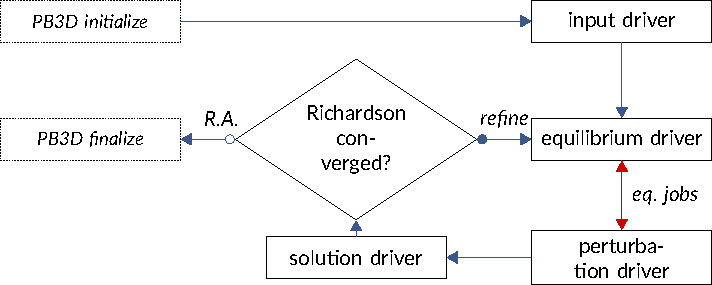
\includegraphics[width=0.7\textwidth]{flowchart}
\doxyfigcaption{{\bfseries Figure} {\bfseries 1} {\bfseries }\+: basic P\+B3D flowchart}
\end{DoxyImage}


Roughly speaking, the main body of the code is taken up by four driver routines\+:
\begin{DoxyItemize}
\item input driver
\item equilibrium driver
\item perturbation driver
\item solution driver
\end{DoxyItemize}

The {\bfseries input driver} sets the other drivers up by reading input options as well as quantities from equilibrium codes, and converting them to the internal P\+B3D format.

The {\bfseries equilibrium driver} uses these input variables to set up equilibrium quantities.
\begin{DoxyItemize}
\item On the one hand these consist of flux equilibrium quantities (stored in a eq\+\_\+vars.\+eq\+\_\+1\+\_\+type) that only depend on the flux coordinates, such as the pressure $p$, the safety factor $q$, etc.
\item On the other hand, they consist of metric equilibrium quantities (stored in a eq\+\_\+vars.\+eq\+\_\+2\+\_\+type) that depend on the angular position as well, such as the metric quantities of the grid $g_{ij} = \vec{e}_i \cdot \vec{e}_j$ and $h_{ij} = \nabla u^i \cdot \nabla u^j$, as well as derived quantities such as the parallel current $\sigma = \frac{\vec{B}\cdot\vec{J}}{B^2}$, etc. \cite{weyens2014theory}
\end{DoxyItemize}

The {\bfseries perturbation driver} uses both types of equation variables to calculate perturbation quantites. Again, there are two types.
\begin{DoxyItemize}
\item The first type of variables are the vectorial perturbation quantities (stored in a x\+\_\+vars.\+x\+\_\+1\+\_\+type), which contains the geodesic component of the perturbation $U = \frac{\nabla \times \vec{B}}{\left|\nabla \psi\right|^2} \cdot \vec{\xi}$ where $\vec{\xi}$ is the perturbation. Also the parallel derivatives of these quantities are calculated.
\item The other type re the tensorial perturbation quantities (stored in a x\+\_\+vars.\+x\+\_\+2\+\_\+type), and it combines the vectorial perturbation quantities with the equilibrium quantities to form the tensorial quantities $\widetilde{PV}_{k,m}^i$ and $\widetilde{KV}_{k,m}^i$ that represent the perturbed potential energy as well as the kinetic energy of the perturbation \cite{weyens2014theory}.
\end{DoxyItemize}

These are also complemented by $\delta_{k,m}^\text{vac}$, the vacuum contribution to the perturbed potential energy (\hyperlink{page_overview_fng1}{1}).

After integrating them along the magnetic field lines, these magnetic integrals form the building blocks of the discretized matrices $\overline{\text{A}}$ and $\overline{\text{B}}$ in the generalized system of eigenvalue equations $\overline{\text{A}} \vec{X} = \lambda \overline{\text{B}}\vec{X}$.

These matrices are set up in the {\bfseries solution driver}, which currently works with the S\+L\+E\+Pc library that is build on the P\+E\+T\+Sc library for sparse linear algebra. After solution, the eigenvalues and -\/vectors are stored appropriately.

Finally, it is checked whether another Richardson level should be attempted or not in {\bfseries Richardson converged?}, and if so, the number of parallel grid points is doubled.\hypertarget{page_overview_overview_jobs}{}\section{Equilibrium \& Perturbation Jobs}\label{page_overview_overview_jobs}
The general code structure explained in \hyperlink{page_overview_overview_PB3D_flowchart}{P\+B3D flowchart} basically comes down to setting up the matrices to be solved for the eigenvalues and eigenvectors. In general, the dimensions of these variables are too large (see the grids in \hyperlink{page_overview_detail_PB3D}{Detailed P\+B3D Flowchart}) for them to fit in memory. A structure of two nested loops is therefore employed in P\+B3D, called {\bfseries jobs}, to keep the memory requirements under a user-\/defined maximum (see {\ttfamily max\+\_\+tot\+\_\+mem} in \hyperlink{page_inputs}{Input variables}).\hypertarget{page_overview_overview_jobs_X}{}\subsection{Perturbation jobs}\label{page_overview_overview_jobs_X}
{\bfseries perturbation jobs} are used to divided the calculation of the tensorial perturbation quantities, which come in pairs of mode numbers. These combinations are blocked, where each block fits in memory. These blocks are the perturbation jobs.

They form the inner loop.

\begin{DoxySeeAlso}{See also}
See \hyperlink{namespacex__ops_a677c88d85fe1bfbf3579a2421ce16f2f}{divide\+\_\+x\+\_\+jobs()}.
\end{DoxySeeAlso}
\hypertarget{page_overview_overview_jobs_eq}{}\subsection{Equilibrium jobs}\label{page_overview_overview_jobs_eq}
As a result the memory still needs to hold all the relevant equilibrium and vectorial perturbation quantities necessary for the individual perturbation jobs during the whole time these jobs are being calculated. {\bfseries equilibrium jobs} are therefore employed in an outer loop to divide these equilibrium and vectorial perturbation quantities in manageable chunks.

To be more precise, the parallel range over which variables are to be integrated in the magnetic integrals (see \hyperlink{page_overview_detail_PB3D}{Detailed P\+B3D Flowchart}), is cut in pieces. The advantage here is that only the results from the sub-\/integrals have to be saved and updated, not the function values themselves.

\begin{DoxySeeAlso}{See also}
See \hyperlink{namespaceeq__ops_a8fae749abe55865d8135fef536a8e8f1}{divide\+\_\+eq\+\_\+jobs()}.
\end{DoxySeeAlso}
\hypertarget{page_overview_detail_PB3D}{}\section{Detailed P\+B3\+D Flowchart}\label{page_overview_detail_PB3D}
The different blocks if figure \hyperlink{page_overview_flowchart_fig}{1} are expanded in table \doxytablelink{page_overview_flowchart_PB3D_tab}{1}. The cells that are typeset in light blue are only performed for the first equilibrium job of either the restart Richardson level, or the first Richardson level if this is not provided. \hypertarget{page_overview_flowchart_PB3D_tab}{}
\tabulinesep=1mm
\begin{longtabu} spread 0pt [c]{*{3}{|X[-1]}|}
\caption{Table 1. detailed P\+B3D flowchart}\label{page_overview_flowchart_PB3D_tab}\\
\hline
\rowcolor{\tableheadbgcolor}\textbf{ variable type }&\textbf{ V\+M\+EC ({\ttfamily eq\+\_\+style = 1}) }&\textbf{ H\+E\+L\+E\+NA ({\ttfamily eq\+\_\+style = 2})   }\\\cline{1-3}
\endfirsthead
\hline
\endfoot
\hline
\rowcolor{\tableheadbgcolor}\textbf{ variable type }&\textbf{ V\+M\+EC ({\ttfamily eq\+\_\+style = 1}) }&\textbf{ H\+E\+L\+E\+NA ({\ttfamily eq\+\_\+style = 2})   }\\\cline{1-3}
\endhead
\multirow{1}{\linewidth}{{\bfseries  P\+B3D initialize }}&\multicolumn{2}{p{(\linewidth-\tabcolsep*3-\arrayrulewidth*2)*2/3}|}{the P\+B3D structure is set up, such as the M\+PI communicator, etc.   }\\\cline{1-3}
\multirow{8}{\linewidth}{{\bfseries  input driver }}&\multicolumn{2}{p{(\linewidth-\tabcolsep*3-\arrayrulewidth*2)*2/3}|}{The arguments are parsed (see \hyperlink{namespacefiles__ops_a051584112f6e4f6e60b0ef824dffbf5e}{parse\+\_\+args()})   }\\\cline{2-3}
&\multicolumn{2}{p{(\linewidth-\tabcolsep*3-\arrayrulewidth*2)*2/3}|}{The input files are opened (see \hyperlink{namespacefiles__ops_a63a81a5a451f787025429878b2cec81b}{open\+\_\+input()} and \hyperlink{page_inputs}{Input variables})   }\\\cline{2-3}
&\multicolumn{2}{p{(\linewidth-\tabcolsep*3-\arrayrulewidth*2)*2/3}|}{The user inputs are processed (see \hyperlink{namespaceinput__ops_a434acca4f59f9dc1d91e04f846133684}{read\+\_\+input\+\_\+opts()})   }\\\cline{2-3}
&\multicolumn{2}{p{(\linewidth-\tabcolsep*3-\arrayrulewidth*2)*2/3}|}{The equilibrium code output is read and converted to the internal P\+B3D format (see \hyperlink{namespaceinput__ops_a577c897cc266961eb40bb5ef747fa077}{read\+\_\+input\+\_\+eq()})   }\\\cline{2-3}
&\multicolumn{2}{p{(\linewidth-\tabcolsep*3-\arrayrulewidth*2)*2/3}|}{Normalization constants are calculated (see \hyperlink{namespaceeq__ops_a09b10d95cd83c89e817664a954f7555d}{calc\+\_\+normalization\+\_\+const()}) and the input is normalized (see \hyperlink{namespaceeq__ops_a1b4c764da73624722d7e76498a2b80a9}{normalize\+\_\+input()})   }\\\cline{2-3}
&\multicolumn{2}{p{(\linewidth-\tabcolsep*3-\arrayrulewidth*2)*2/3}|}{Output files are opened (see \hyperlink{namespacefiles__ops_ad681a9e8083a6f664cf0f9d17ebe279c}{open\+\_\+output()} and \hyperlink{page_outputs}{Code outputs})   }\\\cline{2-3}
&\multicolumn{2}{p{(\linewidth-\tabcolsep*3-\arrayrulewidth*2)*2/3}|}{Input variables are written to H\+D\+F5 output (see \hyperlink{namespaceinput__ops_a84ec7b3833da80ebb36ae0d5ff1a9e0a}{print\+\_\+output\+\_\+in()})  }\\\cline{2-3}
&\multicolumn{2}{p{(\linewidth-\tabcolsep*3-\arrayrulewidth*2)*2/3}|}{Some other variables are broadcasted directly to all the processes using M\+PI (see \hyperlink{namespacempi__ops_a932eba1c998dd7a0f1191b55cd754be3}{broadcast\+\_\+input\+\_\+opts()})   }\\\cline{1-3}
\multirow{14}{\linewidth}{{\bfseries  equilibrium driver } }&normal part of equilibrium grid is set up, as for the angular part, the field-\/lines are necessary which are not yet calculated  &the equilibrium grid is set up equal to the H\+E\+L\+E\+NA output grid   \\\cline{2-3}
&\multicolumn{2}{p{(\linewidth-\tabcolsep*3-\arrayrulewidth*2)*2/3}|}{flux equilibrium quantities (see eq\+\_\+vars.\+eq\+\_\+1\+\_\+type) are calculated (see eq\+\_\+ops.\+calc\+\_\+eq())   }\\\cline{2-3}
&\multicolumn{2}{p{(\linewidth-\tabcolsep*3-\arrayrulewidth*2)*2/3}|}{flux equilibrium quantities are written to H\+D\+F5 output (see eq\+\_\+ops.\+print\+\_\+output\+\_\+eq())   }\\\cline{2-3}
&equilibrium grid is completed by tracing the field lines (see \hyperlink{namespacegrid__ops_a06107dbdfd1dd62e372cc29ab0255bad}{calc\+\_\+ang\+\_\+grid\+\_\+eq\+\_\+b()})  &an additional, field-\/aligned equilibrium grid is set up by tracing the field lines (see \hyperlink{namespacegrid__ops_ad16495ddd320562451c2325bafecf2d8}{setup\+\_\+grid\+\_\+eq\+\_\+b()}), and it is written to H\+D\+F5 output (see \hyperlink{namespacegrid__ops_ab2a8efa54d36500efcabeb9f1aabbcc6}{print\+\_\+output\+\_\+grid()})   \\\cline{2-3}
&the equilibrium grid is written to output  &the equilibrium grid is written to the output  \\\cline{2-3}
&the metric equilibrium variables (see eq\+\_\+vars.\+eq\+\_\+2\+\_\+type) are calculated (see eq\+\_\+ops.\+calc\+\_\+eq())  &the metric equilibrium variables (see eq\+\_\+vars.\+eq\+\_\+2\+\_\+type) are calculated (see eq\+\_\+ops.\+calc\+\_\+eq())  \\\cline{2-3}
&&the metric equilibrium variables are written to the output (see eq\+\_\+ops.\+print\+\_\+output\+\_\+eq())  \\\cline{2-3}
&store equilibrium quantities necessary for vacuum calculation (see store\+\_\+vac())  &store equilibrium quantities necessary for vacuum calculation (see store\+\_\+vac())   \\\cline{2-3}
&possible plot of magnetic field, current density and/or curvature in (field-\/aligned) equilibrium grid (see \hyperlink{namespaceeq__ops_a9dab060a0bbbbaf6c8ccb66e1f5f160b}{b\+\_\+plot()}, \hyperlink{namespaceeq__ops_af611fc0c83d1ab5ed8940d9a1a652d6c}{j\+\_\+plot()}, \hyperlink{namespaceeq__ops_a9ecb744b3812fe838f13c9886307da24}{kappa\+\_\+plot()})  &possible plot of magnetic field, current density and/or curvature in (H\+E\+L\+E\+NA) equilibrium grid (see \hyperlink{namespaceeq__ops_a9dab060a0bbbbaf6c8ccb66e1f5f160b}{b\+\_\+plot()}, \hyperlink{namespaceeq__ops_af611fc0c83d1ab5ed8940d9a1a652d6c}{j\+\_\+plot()}, \hyperlink{namespaceeq__ops_a9ecb744b3812fe838f13c9886307da24}{kappa\+\_\+plot()})  \\\cline{2-3}
&redistribute the equilibrium grid (see \hyperlink{namespacegrid__ops_ab10ef5b486ee3861df2da4e53bc22630}{redistribute\+\_\+output\+\_\+grid()})  &redistribute the equilibrium grid (see \hyperlink{namespacegrid__ops_ab10ef5b486ee3861df2da4e53bc22630}{redistribute\+\_\+output\+\_\+grid()})  \\\cline{2-3}
&\multicolumn{2}{p{(\linewidth-\tabcolsep*3-\arrayrulewidth*2)*2/3}|}{redistribute the flux equilibrium quantities (see eq\+\_\+ops.\+redistribute\+\_\+output\+\_\+eq())   }\\\cline{2-3}
&redistribute the metric equilibrium quantities (see eq\+\_\+ops.\+redistribute\+\_\+output\+\_\+eq())  &redistribute the metric equilibrium quantities (see eq\+\_\+ops.\+redistribute\+\_\+output\+\_\+eq())   \\\cline{2-3}
&&The field-\/aligned equilibrium grid is redistributed (see \hyperlink{namespacegrid__ops_ab10ef5b486ee3861df2da4e53bc22630}{redistribute\+\_\+output\+\_\+grid()})   \\\cline{2-3}
&\multicolumn{2}{p{(\linewidth-\tabcolsep*3-\arrayrulewidth*2)*2/3}|}{possible plot of magnetic field lines in flux surfaces (see \hyperlink{namespacegrid__ops_addd76b7b3be0b51e0863ae0cdfef41e6}{magn\+\_\+grid\+\_\+plot()}) if last equilibrium job   }\\\cline{1-3}
\multirow{11}{\linewidth}{{\bfseries  perturbation driver }}&&the metric equilibrium quantities are inerpolated in the field-\/aligned equilibrium grid (see \hyperlink{namespacehelena__ops_a7796861de18ae7ac9c3aa07a8628be38}{interp\+\_\+hel\+\_\+on\+\_\+grid()})   \\\cline{2-3}
&determine perturbation grid (see \hyperlink{namespacegrid__ops_a1047889ec84da6e56aae619570a16988}{setup\+\_\+grid\+\_\+x()}) and write it to H\+D\+F5 ouput (see \hyperlink{namespacegrid__ops_ab2a8efa54d36500efcabeb9f1aabbcc6}{print\+\_\+output\+\_\+grid()})  &determine perturbation grid (see \hyperlink{namespacegrid__ops_a1047889ec84da6e56aae619570a16988}{setup\+\_\+grid\+\_\+x()}) and write it to H\+D\+F5 ouput (see \hyperlink{namespacegrid__ops_ab2a8efa54d36500efcabeb9f1aabbcc6}{print\+\_\+output\+\_\+grid()})   \\\cline{2-3}
&&set up field-\/aligned perturbation grid and write to output  \\\cline{2-3}
&\multicolumn{2}{p{(\linewidth-\tabcolsep*3-\arrayrulewidth*2)*2/3}|}{set up mode number information (see \hyperlink{namespacex__ops_ad0f44ec07a3b246da23f9aa659683bdf}{setup\+\_\+nm\+\_\+x()}) and check them (see \hyperlink{namespacex__ops_a7d9275e2d927d92548416f21b983b604}{check\+\_\+x\+\_\+modes()}) if first perturbation job  }\\\cline{2-3}
&\multicolumn{2}{p{(\linewidth-\tabcolsep*3-\arrayrulewidth*2)*2/3}|}{possibly plot resonance (see \hyperlink{namespacex__ops_a766228ae0a64f84c10521a013367cfc8}{resonance\+\_\+plot()}) if first perturbation job  }\\\cline{2-3}
&the vectorial perturbation variables (see x\+\_\+vars.\+x\+\_\+1\+\_\+type) are calculated (see x\+\_\+ops.\+calc\+\_\+x())  &the vectorial perturbation variables (see x\+\_\+vars.\+x\+\_\+1\+\_\+type) are calculated (see x\+\_\+ops.\+calc\+\_\+x())   \\\cline{2-3}
&&write vectorial perturbation variables to output (see x\+\_\+ops.\+print\+\_\+output\+\_\+x())   \\\cline{2-3}
&&interpolate vectorial perturbation variables on field-\/aligned grid (see \hyperlink{namespacehelena__ops_a7796861de18ae7ac9c3aa07a8628be38}{interp\+\_\+hel\+\_\+on\+\_\+grid()})   \\\cline{2-3}
&\multicolumn{2}{p{(\linewidth-\tabcolsep*3-\arrayrulewidth*2)*2/3}|}{calculate tensorial perturbation variables (see x\+\_\+ops.\+calc\+\_\+x())   }\\\cline{2-3}
&\multicolumn{2}{p{(\linewidth-\tabcolsep*3-\arrayrulewidth*2)*2/3}|}{calculate magnetic integrals (see \hyperlink{namespacex__ops_a6df79622d1b95d54ab3e542751a5881d}{calc\+\_\+magn\+\_\+ints()})   }\\\cline{2-3}
&\multicolumn{2}{p{(\linewidth-\tabcolsep*3-\arrayrulewidth*2)*2/3}|}{write magnetic integrals to output (see x\+\_\+ops.\+print\+\_\+output\+\_\+x())   }\\\cline{1-3}
\multirow{3}{\linewidth}{{\bfseries  solution driver }}&calculate vacuum (see \hyperlink{namespacevac_a1a1c56e4a52cb5e3f3ee1e307e374c26}{calc\+\_\+vac()})  &calculate vacuum (see \hyperlink{namespacevac_a1a1c56e4a52cb5e3f3ee1e307e374c26}{calc\+\_\+vac()})   \\\cline{2-3}
&\multicolumn{2}{p{(\linewidth-\tabcolsep*3-\arrayrulewidth*2)*2/3}|}{set up the solution grid (see \hyperlink{namespacegrid__ops_ae4f50f7b63e0a8b84dae6b98fd3e5d71}{setup\+\_\+grid\+\_\+sol()}) and write to H\+D\+F5 output (see \hyperlink{namespacegrid__ops_ab2a8efa54d36500efcabeb9f1aabbcc6}{print\+\_\+output\+\_\+grid()})   }\\\cline{2-3}
&\multicolumn{2}{p{(\linewidth-\tabcolsep*3-\arrayrulewidth*2)*2/3}|}{solve system of equations (see \hyperlink{namespaceslepc__ops_ad9d4a9b7275ac5a6b9b35e481a7c1710}{solve\+\_\+ev\+\_\+system\+\_\+slepc()})   }\\\cline{1-3}
\multirow{1}{\linewidth}{{\bfseries  Richardson converged? }}&\multicolumn{2}{p{(\linewidth-\tabcolsep*3-\arrayrulewidth*2)*2/3}|}{check for convergence of Richardson levels by comparing solution eigenvalues (see \hyperlink{namespacerich__ops_ac00cce686d45540b238b3b6e39c9bdeb}{check\+\_\+conv()})   }\\\cline{1-3}
\multirow{1}{\linewidth}{{\bfseries  P\+B3D finalize }}&\multicolumn{2}{p{(\linewidth-\tabcolsep*3-\arrayrulewidth*2)*2/3}|}{clean up   }\\\cline{1-3}
\end{longtabu}
\hypertarget{page_overview_overview_POST}{}\section{P\+O\+S\+T Overview}\label{page_overview_overview_POST}
The P\+O\+ST program for post-\/processing of P\+B3D results consists of just one driver.
\begin{DoxyItemize}
\item In the first part, everything is set up (see \hyperlink{namespacedriver__post_af527706d4e696d4e507443d2f74194ef}{init\+\_\+post()})\+:
\begin{DoxyItemize}
\item This includes initializing the variables written to H\+D\+F5 in P\+B3D.
\item Furthermore, the output grids are created
\item Also, 1-\/D flux plots are produced, which are part of the plots that P\+B3D is able to produce (see {\ttfamily plot\+\_\+flux\+\_\+q}, {\ttfamily plot\+\_\+resonance} and {\ttfamily plot\+\_\+magn\+\_\+grid} in table \doxytablelink{page_outputs_output_plots_tab}{3} in \hyperlink{page_outputs}{Code outputs}) can be created here.
\end{DoxyItemize}
\item After that, new outputs are calculated and plot (see \hyperlink{namespacedriver__post_a33b3c6f9018a0ddc92dce77394b8ab37}{run\+\_\+driver\+\_\+post()})\+:
\begin{DoxyItemize}
\item Quantities are calculated on the output grids.
\item Using these, plots are first produced that do not depend on the solution vector from P\+B3D, and are also part of the plots that P\+B3D is able to produce (see {\ttfamily plot\+\_\+B}, {\ttfamily plot\+\_\+J}, {\ttfamily plot\+\_\+kappa} in table \doxytablelink{page_outputs_output_plots_tab}{3} in \hyperlink{page_outputs}{Code outputs}).
\item Finally, other plots are produced that do depend on these (see {\ttfamily plot\+\_\+sol\+\_\+xi}, {\ttfamily plot\+\_\+sol\+\_\+Q}, {\ttfamily plot\+\_\+\+E\+\_\+rec} in table \doxytablelink{page_outputs_output_plots_tab}{3} in \hyperlink{page_outputs}{Code outputs}).
\end{DoxyItemize}
\end{DoxyItemize}

P\+O\+ST also knows the concept of equilibrium jobs, but not that of perturbation jobs (see \hyperlink{page_overview_overview_jobs}{Equilibrium \& Perturbation Jobs}). This is necessary for larger outputs that quickly overflow memory. The H\+D\+F5 output files are updated at every equilibrium job, but, with reasonable safety, they can already be looked at in a visualizer.

\begin{DoxyNote}{Note}

\begin{DoxyEnumerate}
\item \label{page_overview_fng1}%
\Hypertarget{page_overview_fng1}%
This is not yet implemented. 
\end{DoxyEnumerate}
\end{DoxyNote}

\chapter{Tutorial}
\label{page_tutorial}
\Hypertarget{page_tutorial}
 
    \textit{\scriptsize Footnotes are situated at the end of the chapter}


This page contains a hands-\/on tutorial to get you used to running P\+B3D to calculate 3-\/D ideal linear high-\/n M\+HD stability, and P\+O\+ST to post-\/process the results.

Be sure to check out the \hyperlink{page_installation}{Installation} instruction first.

  
If at any point a routine is not clear, don't hesitate to consult the appendices.
\hypertarget{page_tutorial_tutorial_eq}{}\section{Getting the Equilibrium}\label{page_tutorial_tutorial_eq}
P\+B3D calculates stability of an equilibrium magnetic toroidal configuration. It is written in a modular way to isolate this main task from the actual code that was used to obtain the equilibrium configuration, and the format that this code may use. Currently, two formats are possible\+:
\begin{DoxyItemize}
\item 3-\/D V\+M\+EC \cite{hirshman1983vmec}.
\item Axisymmetric H\+E\+L\+E\+NA \cite{mikhailovskii1997optimization}.
\end{DoxyItemize}

V\+M\+EC is a general 3-\/D code built on an interesting idea\+: The poloidal coordinate $\theta$ is deformed in such as a way to make the Fourier basis that is used to describe the cylindrical coordinates $R(s,\theta,\varphi)$ and $Z(s,\theta,\varphi)$ as narrow as possible, where $s$ is the flux label ( $s=\sqrt{\Psi_\text{tor}/\Psi_{\text{tor,edge}}})$ and $\varphi$ is the regular cylindrical angle (\hyperlink{page_tutorial_fnt1}{1}). This is done by introducing a deformation factor $\lambda(s,\theta,\varphi)$ defined so that the straight-\/field line coordinate $\theta_\text{F}$ is given by $\theta_\text{F} = \theta + \lambda $.

The fact that $R$, $Z$ and $\lambda$ are given as a double Fourier series in $\theta$ and $\zeta$ ensures that the angular derivatives can be done analytically. This property is used in P\+B3D. Apart from that, the flux functions that describe the profiles on the flux surfaces, the rotational transform $\iota(s)$ and pressure $p(s)$, are also returned.

For H\+E\+L\+E\+NA, the situation is different, as this code considers axisymmetric equilibria only. Its output consists, aside from flux functions safety factor $q(\psi)$, presure $p(\psi)$ and toroidal covariant magnetic field $F(\psi)$, where $\psi=\Psi_\text{pol}/\Psi_{\text{pol,edge}}$ is the normalized poloidal angle, of a 2-\/D table for the upper metric factors $h^{\psi\psi}$ and $h^{\psi\theta}$ and the lower metric factor $g_{\zeta\zeta}$. H\+E\+L\+E\+NA uses the same angular coordinates $\theta$ and $\zeta = -\varphi$ as P\+B3D (see \hyperlink{page_tutorial_fnt1}{1}).

\begin{DoxyNote}{Note}
The modular nature of P\+B3D enables easy integration of other equilibrium codes, if necessary.
\end{DoxyNote}
To get the appropriate equilibrium code results into P\+B3D, it suffices to place the output files in the same directory in which P\+B3D is run\+:
\begin{DoxyItemize}
\item for H\+E\+L\+E\+NA, it is a text file, corresponding to the mapping file ({\ttfamily fort.\+12}),
\item for V\+M\+EC, it is the so-\/called {\ttfamily wout} file,
\end{DoxyItemize}

and to specify their names as the second input argument, the first one being the file with user inputs (see \hyperlink{page_tutorial_tutorial_inputs}{Setting Up the Input File}).

\begin{DoxyNote}{Note}
For V\+M\+EC, the {\ttfamily wout} file has to be in Netcdf\textquotesingle{}s {\ttfamily .nc} format. The old {\ttfamily .txt} format is no longer supported.
\end{DoxyNote}
In any case, if you forget how to run the P\+B3D (or P\+O\+ST) programs, you can always just type 
\begin{DoxyCode}
./PB3D --help 
\end{DoxyCode}
 or even just 
\begin{DoxyCode}
./PB3D 
\end{DoxyCode}


\begin{DoxyNote}{Note}
The H\+E\+L\+E\+NA version used here outputs the variables {\ttfamily I\+AS} and {\ttfamily B0} to the mapping file, after the variable {\ttfamily J\+S0} and after the variable {\ttfamily R\+A\+X\+IS}. Some versions do not write these by default. If yours is one of the above, the solution is to change 
\begin{DoxyCode}
write(nmap,8) JS0 
\end{DoxyCode}
 to 
\begin{DoxyCode}
write(nmap,8) JS0, IAS 
\end{DoxyCode}
 and 
\begin{DoxyCode}
write(nmap,8) RAXIS 
\end{DoxyCode}
 to 
\begin{DoxyCode}
write(nmap,8) RAXIS, B0 
\end{DoxyCode}
 in the subroutine {\ttfamily mapping} and recompile and re-\/run H\+E\+L\+E\+NA.
\end{DoxyNote}
\hypertarget{page_tutorial_tutorial_inputs}{}\section{Setting Up the Input File}\label{page_tutorial_tutorial_inputs}
Now that we have the equilibrium files, it is time to have a look at the input file.


\begin{DoxyCodeInclude}
1 &inputdata\_PB3D
2     min\_n\_par\_X             = 500
3     min\_par\_X               = 0.0
4     max\_par\_X               = 2.0
5     alpha                   = 0.0
6     min\_r\_sol               = 0.1
7     max\_r\_sol               = 1.0
8     n\_r\_sol                 = 500
9     prim\_X                  = 10
10     n\_mod\_X                 = 20
11     BC\_style                = 1 1
12     U\_style                 = 3
13     max\_tot\_mem             = 8000
14     max\_it\_rich             = 2
15     use\_normalization       = .true.
16 /
17 //! [some extra options for PB3D]
18     rich\_restart\_lvl        = 1
19     tol\_rich                = 1.0E-4
20     tol\_SLEPC               = 1.0E-8 1.0E-8
21 //! [some extra options for PB3D]
\end{DoxyCodeInclude}


Have a look\+:
\begin{DoxyItemize}
\item {\ttfamily min\+\_\+n\+\_\+par\+\_\+X} is the number of points in the parallel grid.
\item They range from {\ttfamily min\+\_\+par\+\_\+X} to {\ttfamily max\+\_\+par\+\_\+X}. As this is an axisymmetric example, they can simply be chosen to be a fundamental period of $ 2\pi $. For 3-\/D equilibria, this number has to be increased until convergence is reached \cite{Weyens2017PB3D}.
\item {\ttfamily alpha} indicates the field line at which the perturbations are situated.
\item {\ttfamily n\+\_\+r\+\_\+sol} is the number of points in the solution grid, that ranges from {\ttfamily min\+\_\+r\+\_\+sol} to {\ttfamily max\+\_\+r\+\_\+sol} in the P\+B3D normal coordinate (see \hyperlink{namespacenum__vars_ae21ec57b791e369c3558c0eb3da1555b}{num\+\_\+vars.\+use\+\_\+pol\+\_\+flux\+\_\+f}).
\item {\ttfamily n\+\_\+mod\+\_\+X} is the number of resonating Harmonics with {\ttfamily prim\+\_\+X} the primary mode number.
\item {\ttfamily B\+C\+\_\+style(1\+:2)} indicates the style with which the boundary conditions are implemented deep in the plasma and on the plasma edge.
\item {\ttfamily max\+\_\+tot\+\_\+mem} is the total virtual memory that P\+B3D may consume.
\item {\ttfamily use\+\_\+normalization} indicates whether normalization is used (recommended), but it is useful to turn this off for debugging.
\end{DoxyItemize}

\begin{DoxyNote}{Note}
{\ttfamily B\+C\+\_\+style(2)} is currently set to 1, indicating that the mode amplitude is zero at the edge. In the upcoming version of P\+B3D, the vacuum perturbation on the potential energy will be taken into account, which enables other boundary condition styles at the plasma edge.
\end{DoxyNote}
There are also some extra options listed (but not loaded in P\+B3D as they com after the end of the {\ttfamily inputdata\+\_\+\+P\+B3D} block of the Fortran namelist) below\+: 
\begin{DoxyCodeInclude}
18     rich\_restart\_lvl        = 1
19     tol\_rich                = 1.0E-4
20     tol\_SLEPC               = 1.0E-8 1.0E-8
\end{DoxyCodeInclude}
They include\+:
\begin{DoxyItemize}
\item {\ttfamily rich\+\_\+restart\+\_\+lvl} is used to restart a simulation at a certain Richardson level. The Richardson level 1 refers to the first simulation, with the number of parallel points used in the calculation of line integrals along the magnetic field set by {\ttfamily min\+\_\+n\+\_\+par\+\_\+X} (see \doxytablelink{page_inputs_inputs_PB3D_file_tab}{inputs\+\_\+\+P\+B3\+D\+\_\+file\+\_\+tab}). For every subsequent Richardson level, this number is approximately doubled in order to gain a grid size that is twice as fine. The results from these different levels are extrapolated to a theoretically infinitely fine grid. These operations are done in module \hyperlink{namespacerich__ops}{rich\+\_\+ops}.
\item {\ttfamily tol\+\_\+rich} is the tolerance at which Richardson extrapolation is considered to have converged.
\item {\ttfamily tol\+\_\+\+S\+L\+E\+PC} is an array of tolerances used for the different S\+L\+E\+Pc eigenvalue solutions.
\end{DoxyItemize}

There are many, many more input parameters. A short description of these can be found in \hyperlink{page_inputs}{Input variables}.\hypertarget{page_tutorial_tutorial_PB3D}{}\section{Running P\+B3D}\label{page_tutorial_tutorial_PB3D}
This tutorial provides a basic V\+M\+EC equilibrium file to experiment with, called {\ttfamily cbm18}, which represents a simple circular test case designed to be ballooning unstable. \cite{ferraro2010ELMbenchmark} Some properties are given in table \doxytablelink{page_tutorial_tutorial_PB3D_tab}{1}. \hypertarget{page_tutorial_tutorial_PB3D_tab}{}
\tabulinesep=1mm
\begin{longtabu} spread 0pt [c]{*{2}{|X[-1]}|}
\caption{Table 1. equilibrium parameters}\label{page_tutorial_tutorial_PB3D_tab}\\
\hline
toroidal current $I_\text{tot}$  &$1.614MA$   \\\cline{1-2}
$\beta_\text{pol}$  &$0.443 $   \\\cline{1-2}
aspect ratio $\epsilon$  &$1.5 $   \\\cline{1-2}
\end{longtabu}


Put this equilibrium file, as well as the input file in a separate run directory; let\textquotesingle{}s call it {\ttfamily cbm18}.

In order to produce outputs, P\+B3D needs three sub-\/directories in the run directory, called {\ttfamily Data/}, {\ttfamily Scripts/} and {\ttfamily Plots/}.
\begin{DoxyItemize}
\item In {\ttfamily Data/}, datafiles are stored that are used for plots.
\item In {\ttfamily Scripts/}, scripts are generated that use the datafiles from {\ttfamily Data}.
\item The {\ttfamily Plots/}, the resulting plots are located, both for external plots, and for H\+D\+F5 plots that can be read later in visualization software such as Vis\+It or Para\+View. In \hyperlink{page_outputs_output_plots}{Output Plots}, this is explained in more detail.
\end{DoxyItemize}

If these directories are not present, you will receive error message, so go ahead and create them.

We can now run the code using {\ttfamily mpirun}. For example, with 
\begin{DoxyCode}
mpirun -np 4 ./PB3D PB3D.input wout.nc 
\end{DoxyCode}
 4 processes are used. You can find the V\+M\+EC file \href{wout.nc}{\tt here}.

There are optional run-\/time options that can be triggered, such as {\ttfamily --jump\+\_\+to\+\_\+sol}, which can be used to easily change solution preferences, such as discretization order, etc. For an overview, see \hyperlink{page_inputs_inputs_POST_cmd}{Command-\/line inputs}; they are not treated here.

You will see formatted output on the screen, with indentation that consistent indentation according to the depth of a routine in the program. The same output is also written to an output file, unformatted but still indented (see \hyperlink{page_outputs_output_file_log}{Log file}).

The resulting eigenvalues can also be read in a separate output file (see \hyperlink{page_outputs_output_file_EV}{Eigenvalue summary file}).

Take a look at these output files and shuffle a bit with the input parameters if you want. For example, change {\ttfamily n\+\_\+mod\+\_\+X} to another value in order to get a different number Fourier harmonics, or {\ttfamily n\+\_\+r\+\_\+sol} to change the number of normal grid points in the solution. The solution should not change a lot if you have enough harmonics and normal grid poins.

\begin{DoxyNote}{Note}
For V\+M\+EC, the magnetic axis is a bit problematic. It is necessary, therefore, to choose {\ttfamily min\+\_\+r\+\_\+sol} to be slightly larger than 0; 0.\+01 for example.
\end{DoxyNote}
\hypertarget{page_tutorial_tutorial_scripts}{}\section{Run Script Tools}\label{page_tutorial_tutorial_scripts}
P\+B3D comes with a bunch of extra run tools, for which no support is given, but which may be useful for advanced users. In table \doxytablelink{page_tutorial_tutorial_scripts_tab}{2}, an overview is given\+: \hypertarget{page_tutorial_tutorial_scripts_tab}{}
\tabulinesep=1mm
\begin{longtabu} spread 0pt [c]{*{2}{|X[-1]}|}
\caption{Table 2. extra tools}\label{page_tutorial_tutorial_scripts_tab}\\
\hline
{\ttfamily setup\+\_\+\+Run.\+sh}  &Sets up the required files and scripts to run P\+B3D simulations in a folder different than the P\+B3D compilation folder.   \\\cline{1-2}
{\ttfamily run.\+sh}  &modifiable run script that can be used for P\+B3D and P\+O\+ST. It can also run for an array of input variables, which is useful for parameter studies.   \\\cline{1-2}
{\ttfamily change\+\_\+input\+\_\+var.\+sh}  &Changes the value of a variable in a P\+B3D input file. This is used by {\ttfamily run.\+sh}.   \\\cline{1-2}
{\ttfamily extract\+\_\+jobs\+\_\+info.\+sh}  &Extracts the eigenvalues from the results of an input array produced by {\ttfamily run.\+sh}.   \\\cline{1-2}
{\ttfamily inspect\+\_\+\+S\+L\+U\+R\+M\+\_\+jobs.\+sh}  &Finds the directories of all the jobs currently running in S\+L\+U\+RM and in every directory, it gives the tail of {\ttfamily P\+B3\+D.\+out}. The user can decide to cancel the job.   \\\cline{1-2}
\end{longtabu}
\hypertarget{page_tutorial_tutorial_POST}{}\section{Post-\/processing With P\+O\+ST}\label{page_tutorial_tutorial_POST}
P\+O\+ST provides a way to visualize the results from P\+B3D. Many options are possible, and they can be activated using {\ttfamily plot\+\_\+} flags (see \hyperlink{page_inputs_inputs_POST_file}{Input file}).

An example is given in {\ttfamily P\+O\+S\+T.\+input} 
\begin{DoxyCodeInclude}
1 &INPUTDATA\_POST
2     plot\_resonance          = .true.
3     plot\_magn\_grid          = .true.
4     plot\_flux\_q             = .true.
5     plot\_sol\_xi             = .true.
6     plot\_sol\_Q              = .true.
7     plot\_E\_rec              = .true.
8     plot\_B                  = .true.
9     plot\_J                  = .true.
10     plot\_kappa              = .true.
11     min\_r\_plot              = 0.0
12     max\_r\_plot              = 1.0
13     n\_theta\_plot            = 101
14     min\_theta\_plot          = 0.00
15     max\_theta\_plot          = 2.00
16     n\_zeta\_plot             = 1
17     min\_zeta\_plot           = 0.00
18     max\_zeta\_plot           = 0.00
19     POST\_style              = 1
20     plot\_grid\_style         = 0
21     pert\_mult\_factor\_POST   = 0.0000
22     max\_tot\_mem             = 8000
23 /
24 //! [some extra options for POST]
25     ex\_plot\_style           = 2
26     PB3D\_rich\_lvl           = 1
27 //! [some extra options for POST]
\end{DoxyCodeInclude}
 It can be seen that apart from the {\ttfamily plot\+\_\+} flags, there are also
\begin{DoxyItemize}
\item {\ttfamily min\+\_\+r\+\_\+plot} and {\ttfamily max\+\_\+r\+\_\+plot}, which are the direct equivalent of {\ttfamily min\+\_\+r\+\_\+sol} and {\ttfamily max\+\_\+r\+\_\+sol} in P\+B3D.
\item {\ttfamily min\+\_\+theta\+\_\+plot}, {\ttfamily max\+\_\+theta\+\_\+plot} and {\ttfamily n\+\_\+theta\+\_\+plot} which indicate the range of the poloidal variable that is plot, as well as the the number of point. There is an equivalent for the toroidal variable.
\item {\ttfamily P\+O\+S\+T\+\_\+style} that allows the user to change between different styles, such as whether the output grid is chosen to be fill the torus in a regular way, for example, or whether it follows the P\+B3D equilibrium grid.
\item {\ttfamily plot\+\_\+grid\+\_\+style}, subsequently, can be used to change the way in which these grids are produced. For example, they could be changed to slab plots or plots with a straightened toroidal angle.
\item {\ttfamily pert\+\_\+mult\+\_\+factor\+\_\+\+P\+O\+ST} can be used to deform the output grids by the perturbation itself.
\end{DoxyItemize}

Also here, there are also some extra options listed below\+: 
\begin{DoxyCodeInclude}
25     ex\_plot\_style           = 2
26     PB3D\_rich\_lvl           = 1
\end{DoxyCodeInclude}
They include\+:
\begin{DoxyItemize}
\item {\ttfamily ex\+\_\+plot\+\_\+style} to indicate which program is to be used for external plotting. Changing it to 2 would engage Bokeh and Mayavi.
\item {\ttfamily P\+B3\+D\+\_\+rich\+\_\+lvl} can be optionally employed to specify explicitely which Richardson level to use for the post-\/processing.
\end{DoxyItemize}

All of these options are explained in \hyperlink{page_inputs_inputs_POST_file}{Input file}. Again, there are also run-\/time options that can be found in \hyperlink{page_inputs_inputs_POST_cmd}{Command-\/line inputs}.

Now, run the P\+O\+ST program, for example using 4 M\+PI processes\+: 
\begin{DoxyCode}
mpirun -np 4 ./POST POST.input PB3D\_out.h5 
\end{DoxyCode}


An interesting output is the energy reconstruction, which is activated with {\ttfamily plot\+\_\+\+E\+\_\+rec}. This calculation reinserts the solution normal mode into the perturbed plasma potential terms, in order to check whether the Rayleigh quotient still holds, and to see which terms are dominant and which ones are less important. The results are stored in a separate files as well (see \hyperlink{page_outputs_output_file_E_rec}{Energy reconstruction file}).

If {\ttfamily --do\+\_\+execute\+\_\+command\+\_\+line} was not explicitely used, the actual external plot programs are not used yet, but their usage is given in a shell commands script file (see \hyperlink{page_outputs_output_file_shell}{Shell commands file}). Run this shell with 
\begin{DoxyCode}
./POST\_shell\_commands.sh 
\end{DoxyCode}


If everything is okay, you should now see output in the {\ttfamily Plots/} folder. If an error occurs, please verfiy whether you have appropriate versions of the external plot programs (i.\+e. Gnu\+Plot, Bokeh, ...)

Also, open some of the {\ttfamily .xmf} files in Vis\+It or Para\+View to explore these plots.

To finish this tutorial, feel free to adjust some input parameters. For example, you can change the output grid to become 3-\/D by setting {\ttfamily n\+\_\+zeta\+\_\+plot} and {\ttfamily max\+\_\+zeta\+\_\+plot}, or you could deform it using {\ttfamily pert\+\_\+mult\+\_\+factor\+\_\+\+P\+O\+ST}.

\begin{DoxyNote}{Note}

\begin{DoxyEnumerate}
\item \label{page_tutorial_fnt1}%
\Hypertarget{page_tutorial_fnt1}%
The cylindrical angle $\varphi$ is often the inverse of the one used in nuclear fusion research, as it can lead to left-\/handed coordinate systems. In V\+M\+EC, it is opted to use it anyway, so it has a left-\/handed coordinate system. The poloidal angle is chosen to be anticlockwise if you look at a cross-\/section of the plasma that lies to the right of the $Z$-\/axis with the $Z$-\/axis pointing up, as in P\+B3D. In P\+B3D, however, the toroidal angle $\zeta = - \varphi$ is chosen as the inverse of the cylindrical angle, so it is right-\/handed. 
\end{DoxyEnumerate}
\end{DoxyNote}

\chapter{Installation}
\label{page_installation}
\Hypertarget{page_installation}
\hypertarget{page_installation_installation_introduction}{}\section{Introduction}\label{page_installation_installation_introduction}
P\+B3D is written in Fortran, and makes use of multiple numerical libraries\+:
\begin{DoxyItemize}
\item \href{http://www.netlib.org/lapack/}{\tt blas / lapack}
\begin{DoxyItemize}
\item for basic linear algebra
\end{DoxyItemize}
\item \href{http://www.netlib.org/scalapack/}{\tt pblas / blacs / scalapack}
\begin{DoxyItemize}
\item for parallelized basic linear algebra
\end{DoxyItemize}
\item \href{https://www.hdfgroup.org/HDF5/}{\tt H\+D\+F5}
\begin{DoxyItemize}
\item for storage files
\item works in parallel
\end{DoxyItemize}
\item \href{https://www.unidata.ucar.edu/software/netcdf/}{\tt Net\+C\+DF}
\begin{DoxyItemize}
\item to read input of V\+M\+EC
\item sequential
\end{DoxyItemize}
\item \href{https://www.mcs.anl.gov/petsc/}{\tt P\+E\+T\+Sc} / \href{http://slepc.upv.es/}{\tt S\+L\+E\+Pc}
\begin{DoxyItemize}
\item for linear algebra of large, sparse matrices
\item can reach $\sim \mathcal{O} (n)$ complexity
\item Minimal installation instructions\+:
\begin{DoxyEnumerate}
\item Configure P\+E\+T\+Sc using {\ttfamily ./configure P\+E\+T\+S\+C\+\_\+\+A\+R\+CH=complex C\+O\+P\+T\+F\+L\+A\+GS=-\/\+O3 C\+X\+X\+O\+P\+T\+F\+L\+A\+GS=-\/\+O3 F\+O\+P\+T\+F\+L\+A\+GS=-\/\+O3 \textbackslash{}}~\newline
 {\ttfamily -\/-\/with-\/scalar-\/type=complex \textbackslash{}}~\newline
 {\ttfamily -\/-\/download-\/metis \textbackslash{}}~\newline
 {\ttfamily -\/-\/download-\/mumps \textbackslash{}}~\newline
 {\ttfamily -\/-\/download-\/parmetis \textbackslash{}}~\newline
 {\ttfamily -\/-\/with-\/scalapack-\/lib=\char`\"{}-\/\+L\mbox{[}\+S\+C\+A\+L\+A\+P\+A\+C\+K\+D\+I\+R\mbox{]}/lib -\/lscalapack\char`\"{} \textbackslash{}}~\newline
 {\ttfamily -\/-\/with-\/valgrind-\/dir=/usr \textbackslash{}}~\newline
 {\ttfamily -\/-\/with-\/debugging=no \textbackslash{}}~\newline
 {\ttfamily -\/-\/with-\/fortran-\/kernels=1}~\newline
 (If you want debug, remove {\ttfamily -\/-\/with-\/debugging=no}, {\ttfamily -\/-\/with-\/fortran-\/kernels=1}, C\+O\+P\+T\+S\+F\+L\+A\+GS, C\+X\+X\+O\+P\+T\+F\+L\+A\+GS and F\+O\+P\+T\+F\+L\+A\+GS, and change P\+E\+T\+S\+C\+\_\+\+A\+R\+CH to {\ttfamily debug-\/complex}.)~\newline
 (If you use a different H\+D\+F5, add {\ttfamily -\/-\/with-\/hdf5-\/dir=\mbox{[}H\+D\+F5\+D\+IR\mbox{]}}.)
\item follow instructions to do makes and tests.
\item Set global variables {\ttfamily export S\+L\+E\+P\+C\+\_\+\+D\+IR=\mbox{[}S\+L\+E\+PC D\+IR\mbox{]}}, {\ttfamily export P\+E\+T\+S\+C\+\_\+\+D\+IR=\mbox{[}P\+E\+T\+S\+C\+\_\+\+D\+IR\mbox{]}} and {\ttfamily export P\+E\+T\+S\+C\+\_\+\+A\+R\+CH=\mbox{[}debug-\/\mbox{]}complex} (depending on whether it is debug or not).
\item Configure S\+L\+E\+Pc using {\ttfamily ./configure}
\item follow instructions to do makes and tests
\end{DoxyEnumerate}
\end{DoxyItemize}
\item \href{http://portal.nersc.gov/project/sparse/strumpack/}{\tt Strum\+Pack}
\begin{DoxyItemize}
\item for linear algebra of structured matrices \cite{Ambikasaran2013}
\item can reach $\sim \mathcal{O} (n \log(n))$ complexity
\end{DoxyItemize}
\item \href{http://vmecwiki.pppl.wikispaces.net/STELLOPT+Compilation}{\tt libstell}
\begin{DoxyItemize}
\item part of Stellopt suite, which contains V\+M\+EC
\item provides routines to read V\+M\+EC output data
\end{DoxyItemize}
\item \href{https://w3.pppl.gov/ntcc/PSPLINE/}{\tt pspline}
\begin{DoxyItemize}
\item Princeton Spline and Hermite Cubic Interpolation Routines
\item Minimal installation instructions\+:
\begin{DoxyEnumerate}
\item Export {\ttfamily F\+F\+L\+A\+GS} en {\ttfamily C\+F\+L\+A\+GS} if you want to optimize\+:
\begin{DoxyItemize}
\item copy {\ttfamily share/\+Make.\+overwrite.\+sample} to {\ttfamily share/\+Make.\+overwrite}
\item Run the gmake below and note the flags, then edit these and put them in {\ttfamily share/\+Make.\+overwrite}
\item if G\+CC\+:
\begin{DoxyItemize}
\item {\ttfamily F\+F\+L\+A\+GS = -\/c -\/\+O3 -\/m64 -\/fno-\/range-\/check -\/fdollar-\/ok -\/cpp ; export F\+F\+L\+A\+GS}
\item {\ttfamily C\+F\+L\+A\+GS = -\/c -\/\+O3 -\/m64 ; export C\+F\+L\+A\+GS}
\item {\ttfamily C\+X\+X\+F\+L\+A\+GS = -\/c -\/\+O3 -\/m64 ; export C\+X\+X\+F\+L\+A\+GS}
\end{DoxyItemize}
\item if Intel\+:
\begin{DoxyItemize}
\item {\ttfamily F\+F\+L\+A\+GS = -\/c -\/\+O3 -\/nowarn -\/ftz -\/auto-\/scalar -\/traceback -\/align dcommons}
\item {\ttfamily M\+P\+I\+\_\+\+F\+F\+L\+A\+GS = -\/c -\/\+O3 -\/nowarn -\/ftz -\/traceback -\/align dcommons -\/auto-\/scalar} (possibly add FC=mpiifort, {\ttfamily C\+XX=mpicpc}, {\ttfamily CC=mpiicc} if on a cluster)
\end{DoxyItemize}
\end{DoxyItemize}
\item Compile with {\ttfamily gmake N\+E\+T\+C\+D\+F\+\_\+\+D\+IR= F\+O\+R\+T\+R\+A\+N\+\_\+\+V\+A\+R\+I\+A\+NT=\mbox{[}V\+A\+R\+I\+A\+NT\mbox{]}} with {\ttfamily \mbox{[}V\+A\+R\+I\+A\+NT\mbox{]}} either {\ttfamily G\+CC} or {\ttfamily Intel} (add {\ttfamily D\+E\+B\+UG=1} and remove the F\+L\+A\+GS if debug wanted). Possibly also add {\ttfamily O\+BJ=\$\mbox{[}C\+O\+M\+P\+\_\+\+D\+IR\mbox{]}} if on a cluster, with {\ttfamily \mbox{[}C\+O\+M\+P\+\_\+\+D\+IR\mbox{]}} the directory where to put the resulting library.
\item Run tests from {\ttfamily R\+E\+A\+D\+M\+E\+\_\+\+Pspline}.
\end{DoxyEnumerate}
\end{DoxyItemize}
\end{DoxyItemize}

They should probably be installed in this order. On linux distributions such as Ubuntu, they may be available as packages.

Furthermore, P\+B3D comes bundled with some other, smaller libraries\+:
\begin{DoxyItemize}
\item \href{http://www.netlib.org/fftpack/}{\tt fftpack}
\begin{DoxyItemize}
\item to calculate the fast Fourier transform
\end{DoxyItemize}
\item \href{http://foul.sourceforge.net/}{\tt foul}
\begin{DoxyItemize}
\item the Fortran Output Library
\end{DoxyItemize}
\end{DoxyItemize}

These do not have to be installed separately.\hypertarget{page_installation_installation_compilation}{}\section{Compilation}\label{page_installation_installation_compilation}
When all dependencies are satisfied, the program is then compiled in the standard way\+:
\begin{DoxyItemize}
\item Including the headers of all the libraries in the compilation of the object files\+:
\begin{DoxyItemize}
\item This is done using {\ttfamily -\/I\mbox{[}path\+\_\+to\+\_\+library\mbox{]}}.
\item Make sure you add the {\ttfamily -\/o} option to create only object files.
\end{DoxyItemize}
\item Linking with the actual libraries
\begin{DoxyItemize}
\item This is done using {\ttfamily -\/L\mbox{[}path\+\_\+to\+\_\+library\mbox{]} -\/l\mbox{[}library\+\_\+name\mbox{]}}.
\end{DoxyItemize}
\end{DoxyItemize}\hypertarget{page_installation_installation_makefile}{}\section{Makefile Example}\label{page_installation_installation_makefile}

\begin{DoxyCodeInclude}
1 ##############################################################################
2 #
3 #   Example makefile for the program PB3D (Peeling Ballooning in 3D)
4 #   \(\backslash\)author Author: Toon Weyens
5 #
6 #   Don't forget to set the directories:
7 #       - LIBSTELL\_DIR
8 #       - HDF5\_DIR
9 #       - NETCDFF\_DIR (note: Fortran library)
10 #       - PETSC\_DIR
11 #       - SLEPC\_DIR
12 #       - STRUMPACK\_DIR
13 ##############################################################################
14 
15 ##############################################################################
16 #   Include
17 ##############################################################################
18 ## [PETSc and SLEPc trick]
19 include  $(PETSC\_DIR)/lib/petsc/conf/variables
20 include  $(SLEPC\_DIR)/lib/slepc/conf/slepc\_variables
21 ## [PETSc and SLEPc trick]
22 
23 ## [PETSc and SLEPc trick inc]
24 INCLUDE = $(PETSC\_FC\_INCLUDES) $(SLEPC\_INCLUDE)
25 ## [PETSc and SLEPc trick inc]
26 ## [Libstell special]
27 INCLUDE += -I$(LIBSTELL\_DIR)/libstell\_dir
28 ## [Libstell special]
29 INCLUDE += -I$(STRUMPACK\_DIR)/include
30 ## [PB3D include]
31 INCLUDE += -I$(PB3D\_DIR)/include
32 ## [PB3D include]
33 INCLUDE += -I/usr/include/hdf5/openmpi
34 
35 ##############################################################################
36 #   Link
37 ##############################################################################
38 ## [PB3D libraries]
39 LIB\_INTERNAL = libdfftpack.a libfoul.a libbspline.a
40 ## [PB3D libraries]
41 
42 LINK := $(LIB\_INTERNAL)
43 
44 ## [PETSc and SLEPc trick lib]
45 LINK += $(PETSC\_LIB)
46 LINK += $(SLEPC\_LIB)
47 ## [PETSc and SLEPc trick lib]
48 LINK += $(LIBSTELL\_DIR)/libstell.a
49 LINK += -L$(STRUMPACK\_DIR)/lib -lstrumpack
50 LINK += -L$(HDF5\_DIR) -lhdf5\_fortran -lhdf5
51 LINK += -L$(NETCDFF\_DIR)/lib -lnetcdff
52 LINK += -Wl,-R$(NETCDFF\_DIR)/lib
53 LINK += -lscalapack -lblacs -lblas -lm
54 LINK += -lstdc++ -lmpi\_cxx
55 
56 
57 ##############################################################################
58 #   Compiler
59 ##############################################################################
60 COMPILER=mpifort
61 
62 
63 ##############################################################################
64 #   Linker
65 ##############################################################################
66 LINKER=mpifort
67 
68 
69 ##############################################################################
70 #   Compiler flags
71 #   options (used with -D[name]):
72 #       ldebug: debug
73 #       lIB: infiniband
74 #       lwith\_gnu: use GNU compiler [default]
75 #       lwith\_intel: use INTEL compiler, (checked for version 12.0.2)
76 #   note: INTEL warning 6536 is suppressed, which informs about extra "USE".
77 #   note: INTEL warning 6843 is suppressed, which informs about empty
78 #       intent(out) variables
79 ##############################################################################
80 COMP\_FLAGS = -finit-real=snan -g -Og -Wall -Wextra -pedantic \(\backslash\)
81     -fimplicit-none -fbacktrace -fno-omit-frame-pointer \(\backslash\)
82     -fcheck=all -cpp -Dldebug# debug, profiling with gprof2dot, GCC
83 #COMP\_FLAGS = -O3 -fbacktrace -g -fimplicit-none -fno-omit-frame-pointer \(\backslash\)
84     #-cpp# optimized, GCC
85 
86 #COMP\_FLAGS = -O0 -DlIB -Dldebug -g -heap-arrays 100 -recursive \(\backslash\)
87     #-ftrapuv -check bounds -check uninit -traceback -implicitnone \(\backslash\)
88     #-fno-omit-frame-pointer -cpp -Dlwith\_intel -diag-disable 6536 \(\backslash\)
89     #-diag-disable 6843# debug, profiling with gprof2dot, INTEL
90 #COMP\_FLAGS = -O3 -DlIB -traceback -g -heap-arrays 100 -recursive \(\backslash\)
91     #-implicitnone -fno-omit-frame-pointer -cpp -Dlwith\_intel \(\backslash\)
92     #-diag-disable 6536 -diag-disable 6843# optimized, INTEL
93 
94 COMP\_FLAGS\_EX= -O2 -w
95 
96 COMP\_FLAGS\_F= -O2 -funroll-loops -fexpensive-optimizations
97 
98 
99 ##############################################################################
100 #   Link flags
101 ##############################################################################
102 LINK\_FLAGS = -fPIC -finit-real=snan# debug
103 #LINK\_FLAGS = -fPIC# optimized
104 
105 
106 ##############################################################################
107 #   Prepare
108 ##############################################################################
109 # Add "Modules" and "Libraries" to the search path for the prerequisites
110 VPATH = Modules:Libraries
111 
112 # Contains list of source files (.o) and dependencies
113 DEPLIST = PB3D.dep
114 OBJLIST = ObjectList# defines "ObjectFiles"
115 
116 # Includes source files and dependency list
117 include $(DEPLIST)# Dependencies of all the objects
118 include $(OBJLIST)# Names of all the objects
119 
120 
121 ##############################################################################
122 #   Rules
123 ##############################################################################
124 all:    PB3D POST
125 
126 PB3D:   $(ObjectFiles) $(LIB\_INTERNAL) PB3D.o
127     $(LINKER) -o $@ $(ObjectFiles) PB3D.o $(LINK) $(LINK\_FLAGS)
128 
129 POST:   $(ObjectFiles) $(LIB\_INTERNAL) POST.o
130     $(LINKER) -o $@ $(ObjectFiles) POST.o $(LINK) $(LINK\_FLAGS)
131 
132 libdfftpack.a:  dfft.o
133     ar -rcs libdfftpack.a dfft.o
134 
135 libfoul.a:  foul.o
136     ar -rcs libfoul.a foul.o
137 
138 libbspline.a:   bspline\_sub\_module.o
139     ar -rcs libbspline.a bspline\_sub\_module.o
140 
141 %.o: %.f90
142     $(COMPILER) $(INCLUDE) $(COMP\_FLAGS) -c $<
143 
144 %.o: %.f
145     $(COMPILER) $(COMP\_FLAGS\_F) -c $<
146 
147 dfft.o: dfft.f
148     $(COMPILER) $(COMP\_FLAGS\_EX) -c $<
149 
150 foul.o: foul.f90
151     $(COMPILER) $(COMP\_FLAGS\_EX) -c $<
152 
153 bspline\_sub\_module.o: bspline\_sub\_module.f90
154     $(COMPILER) $(COMP\_FLAGS\_EX) -c $<
155 
156 clean:
157     @rm -f *.o *.a *.mod *~ fort.* 
158 
159 clean\_all:
160     @rm -f *.o *.mod *~ fort.* PB3D POST
\end{DoxyCodeInclude}


\begin{DoxyNote}{Note}

\begin{DoxyEnumerate}
\item P\+E\+T\+Sc and S\+L\+E\+Pc don\textquotesingle{}t like to be included in another makefile. The trick is to include two files\+: 
\begin{DoxyCodeInclude}
19 include  $(PETSC\_DIR)/lib/petsc/conf/variables
20 include  $(SLEPC\_DIR)/lib/slepc/conf/slepc\_variables
\end{DoxyCodeInclude}
 which will load the variables {\ttfamily P\+E\+T\+S\+C\+\_\+\+F\+C\+\_\+\+I\+N\+C\+L\+U\+D\+ES} and {\ttfamily S\+L\+E\+P\+C\+\_\+\+I\+N\+C\+L\+U\+DE}, used in 
\begin{DoxyCodeInclude}
24 INCLUDE = $(PETSC\_FC\_INCLUDES) $(SLEPC\_INCLUDE)
\end{DoxyCodeInclude}
 as well as the variables {\ttfamily P\+E\+T\+S\+C\+\_\+\+L\+IB} and {\ttfamily S\+L\+E\+P\+C\+\_\+\+L\+IB}, used in 
\begin{DoxyCodeInclude}
45 LINK += $(PETSC\_LIB)
46 LINK += $(SLEPC\_LIB)
\end{DoxyCodeInclude}

\item There are versions of libstell that do not use the standard convention. In this case you have to look for the {\ttfamily $\ast$.mod} files. In the example makefile this is done with 
\begin{DoxyCodeInclude}
27 INCLUDE += -I$(LIBSTELL\_DIR)/libstell\_dir
\end{DoxyCodeInclude}
 instead of the standard {\ttfamily inc} directory.
\item In 
\begin{DoxyCodeInclude}
31 INCLUDE += -I$(PB3D\_DIR)/include
\end{DoxyCodeInclude}
 there are includefiles that contain macros and wrappers specifically for P\+B3D.
\item In 
\begin{DoxyCodeInclude}
39 LIB\_INTERNAL = libdfftpack.a libfoul.a libbspline.a
\end{DoxyCodeInclude}
 linking is done with external libraries that are bundled with P\+B3D. 
\end{DoxyEnumerate}
\end{DoxyNote}

\chapter{Todo List}
\label{todo}
\Hypertarget{todo}

\begin{DoxyRefList}
\item[Module \mbox{\hyperlink{namespacevac__ops}{vac\+\_\+ops}} ]\label{todo__todo000001}%
\Hypertarget{todo__todo000001}%
The vacuum part of P\+B3D is still under construction and not usable yet.  
\item[Subprogram \mbox{\hyperlink{namespacevac__ops_a7e3f92fbe9fa6cf3de6ac301676b96d1}{vac\+\_\+ops::calc\+\_\+gh}} (vac, n\+\_\+r\+\_\+in, lims\+\_\+r\+\_\+in, x\+\_\+vec\+\_\+in, G\+\_\+in, H\+\_\+in)]\label{todo__todo000002}%
\Hypertarget{todo__todo000002}%
For 3-\/D vacuums, step sizes are constant. Subsequent Richardson levels should therefore make use of the fact that the contribution to the points inherited from the previous levels can be just scaled by 1/2 and do not need to be recalculated. Currently, the copy is done correctly in \mbox{\hyperlink{namespacevac__utilities_a8e7889688701f6ac2fd2c60cdee2b96a}{interlaced\+\_\+vac\+\_\+copy()}}, but they are afterwards overwritten.
\end{DoxyRefList}
\begin{appendices}
\appendixpage
\noappendicestocpagenum
\addappheadtotoc
\chapter{Programs}
\hypertarget{POST_8f90}{}\section{/opt/\+P\+B3\+D/\+P\+O\+ST.f90 Program Rerefence}
\label{POST_8f90}\index{/opt/\+P\+B3\+D/\+P\+O\+S\+T@{/opt/\+P\+B3\+D/\+P\+O\+S\+T}}



Peeling Ballooning in 3D\+: postprocessing. 

\begin{DoxyAuthor}{Author}
Toon Weyens, Contact\+: \href{mailto:weyenst@gmail.com}{\tt weyenst@gmail.\+com} 
\end{DoxyAuthor}
\begin{DoxyVersion}{Version}
2.\+37 
\end{DoxyVersion}
\begin{DoxyDate}{Date}
2012-\/2018 
\end{DoxyDate}
\begin{DoxyCopyright}{Copyright}
G\+NU General Public License. 
\end{DoxyCopyright}
\begin{DoxySeeAlso}{See also}
References\+: \cite{weyens2014theory} \cite{Weyens2017PB3D} 
\end{DoxySeeAlso}


Definition at line 27 of file P\+O\+S\+T.

Here is the call graph for this function\+:\nopagebreak
\begin{figure}[H]
\begin{center}
\leavevmode
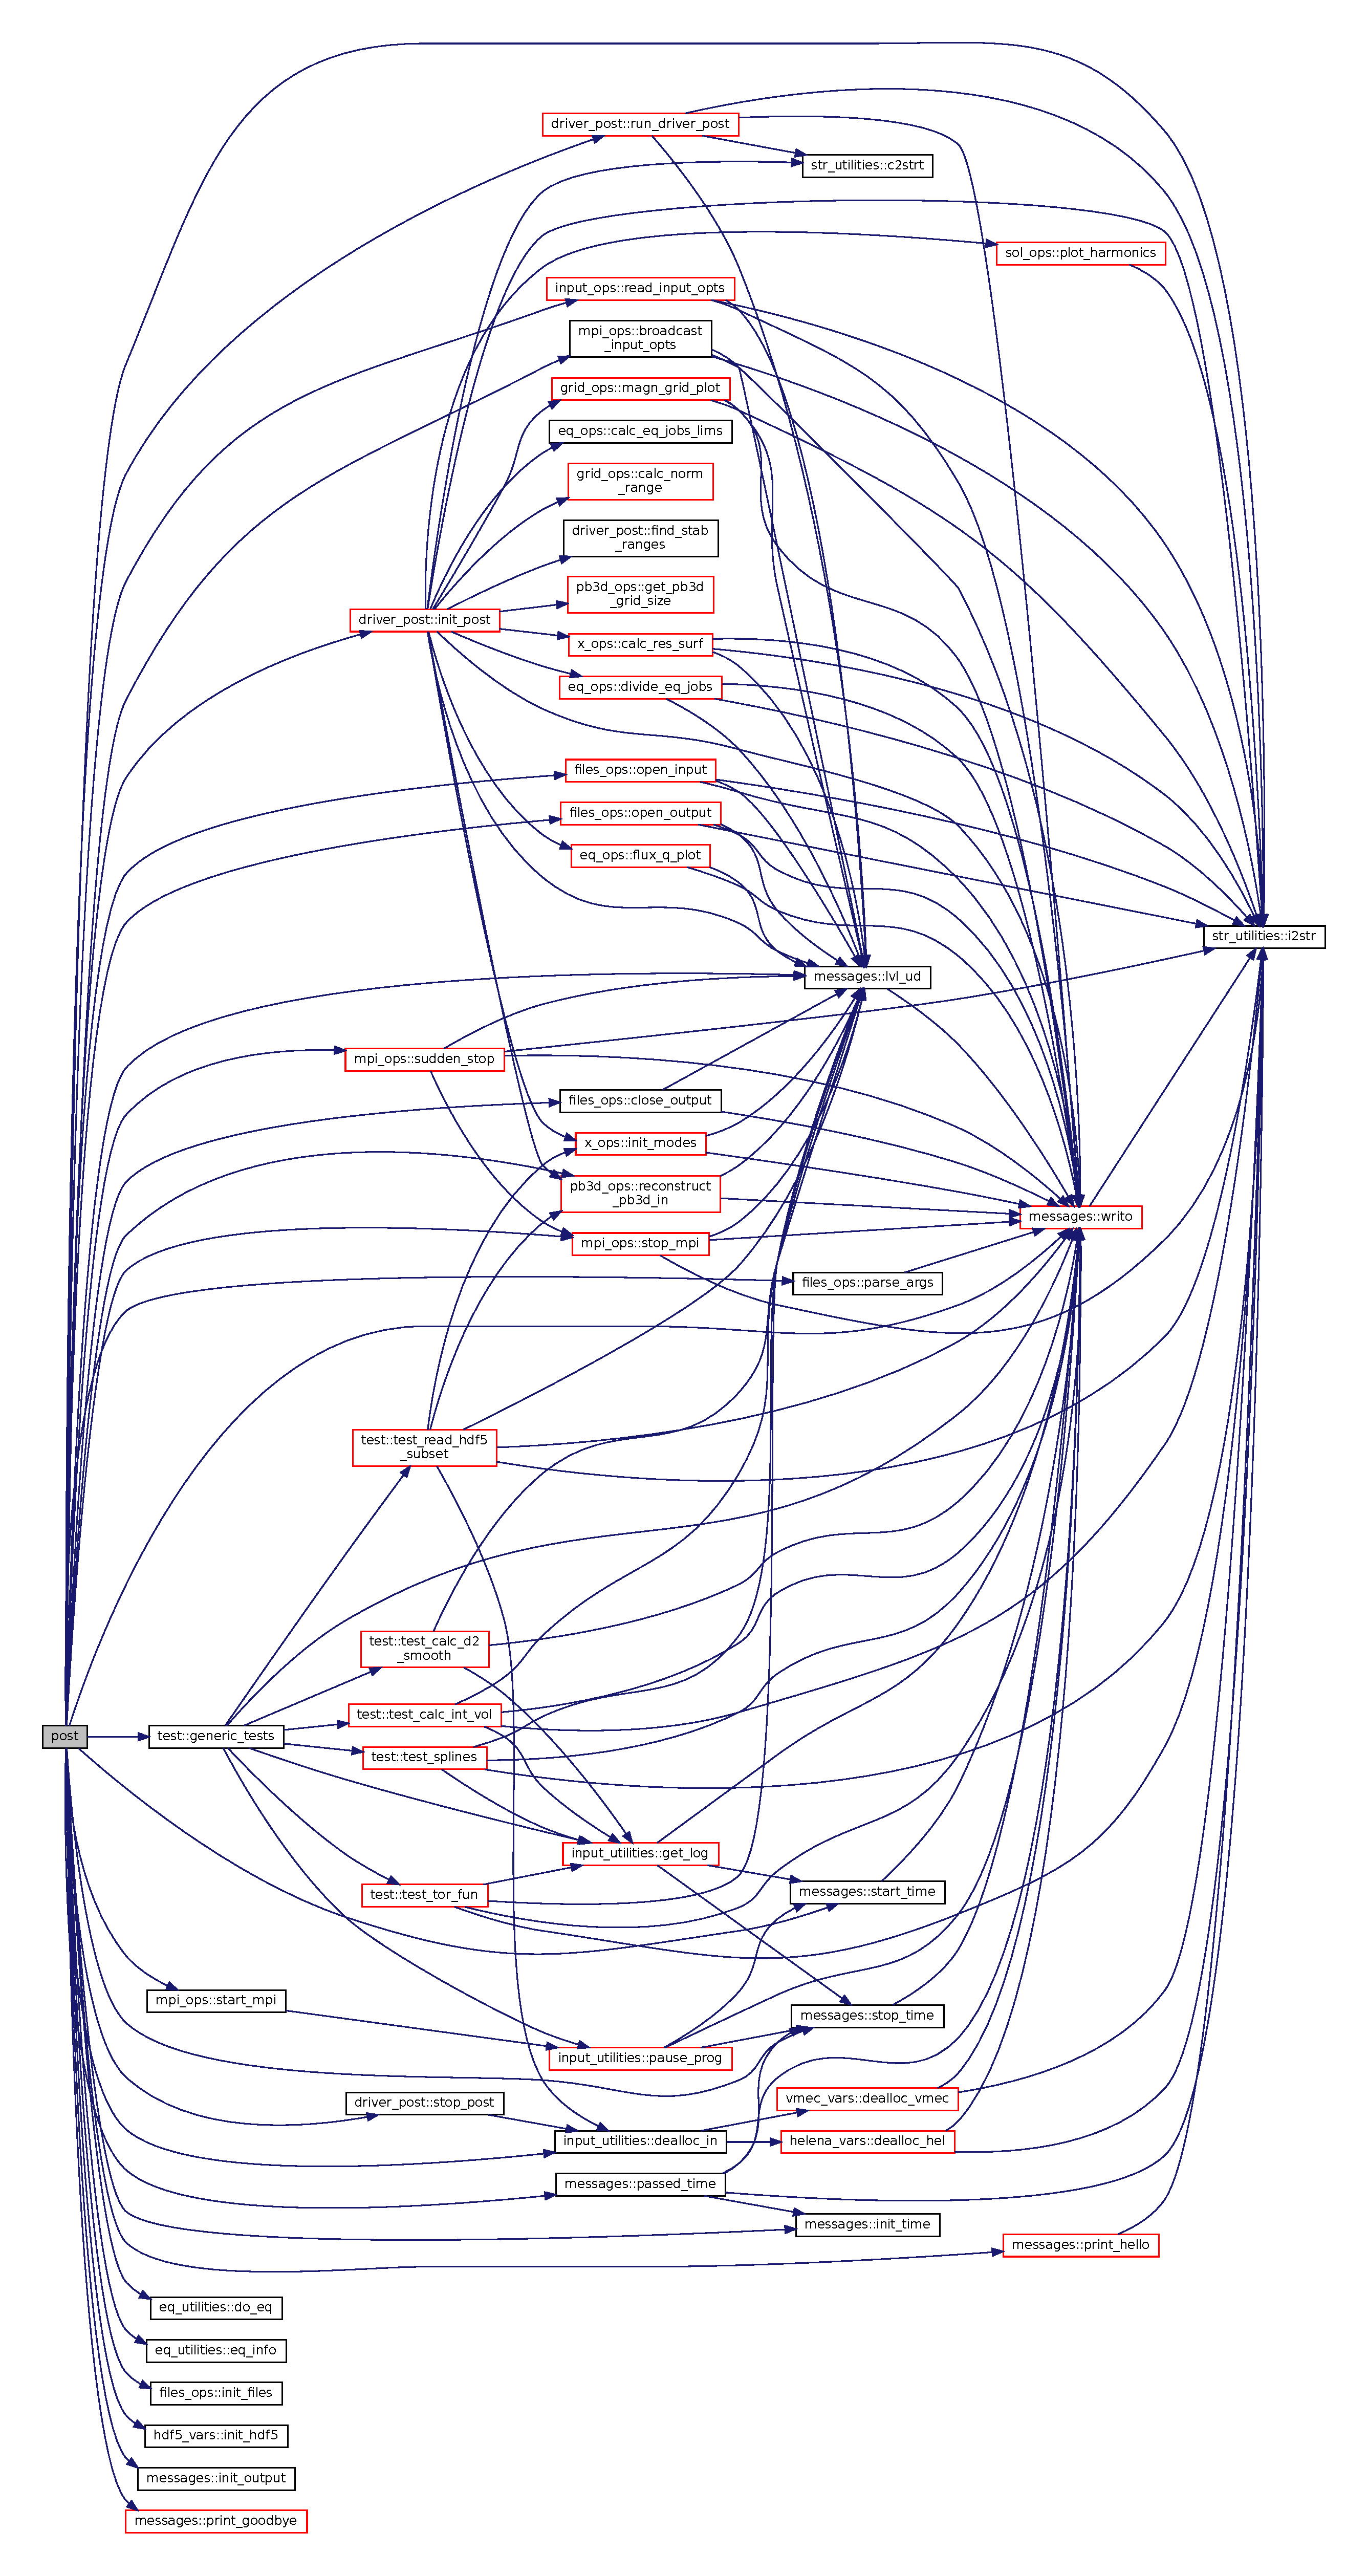
\includegraphics[height=550pt]{POST_8f90_ac289b64ac4671fea0b4f2298ba1188a1_cgraph}
\end{center}
\end{figure}

\hypertarget{PB3D_8f90}{}\section{/opt/\+P\+B3\+D/\+P\+B3D.f90 Program Rerefence}
\label{PB3D_8f90}\index{/opt/\+P\+B3\+D/\+P\+B3\+D@{/opt/\+P\+B3\+D/\+P\+B3\+D}}



Definition at line 24 of file P\+B3\+D.

Here is the call graph for this function\+:
\nopagebreak
\begin{figure}[H]
\begin{center}
\leavevmode
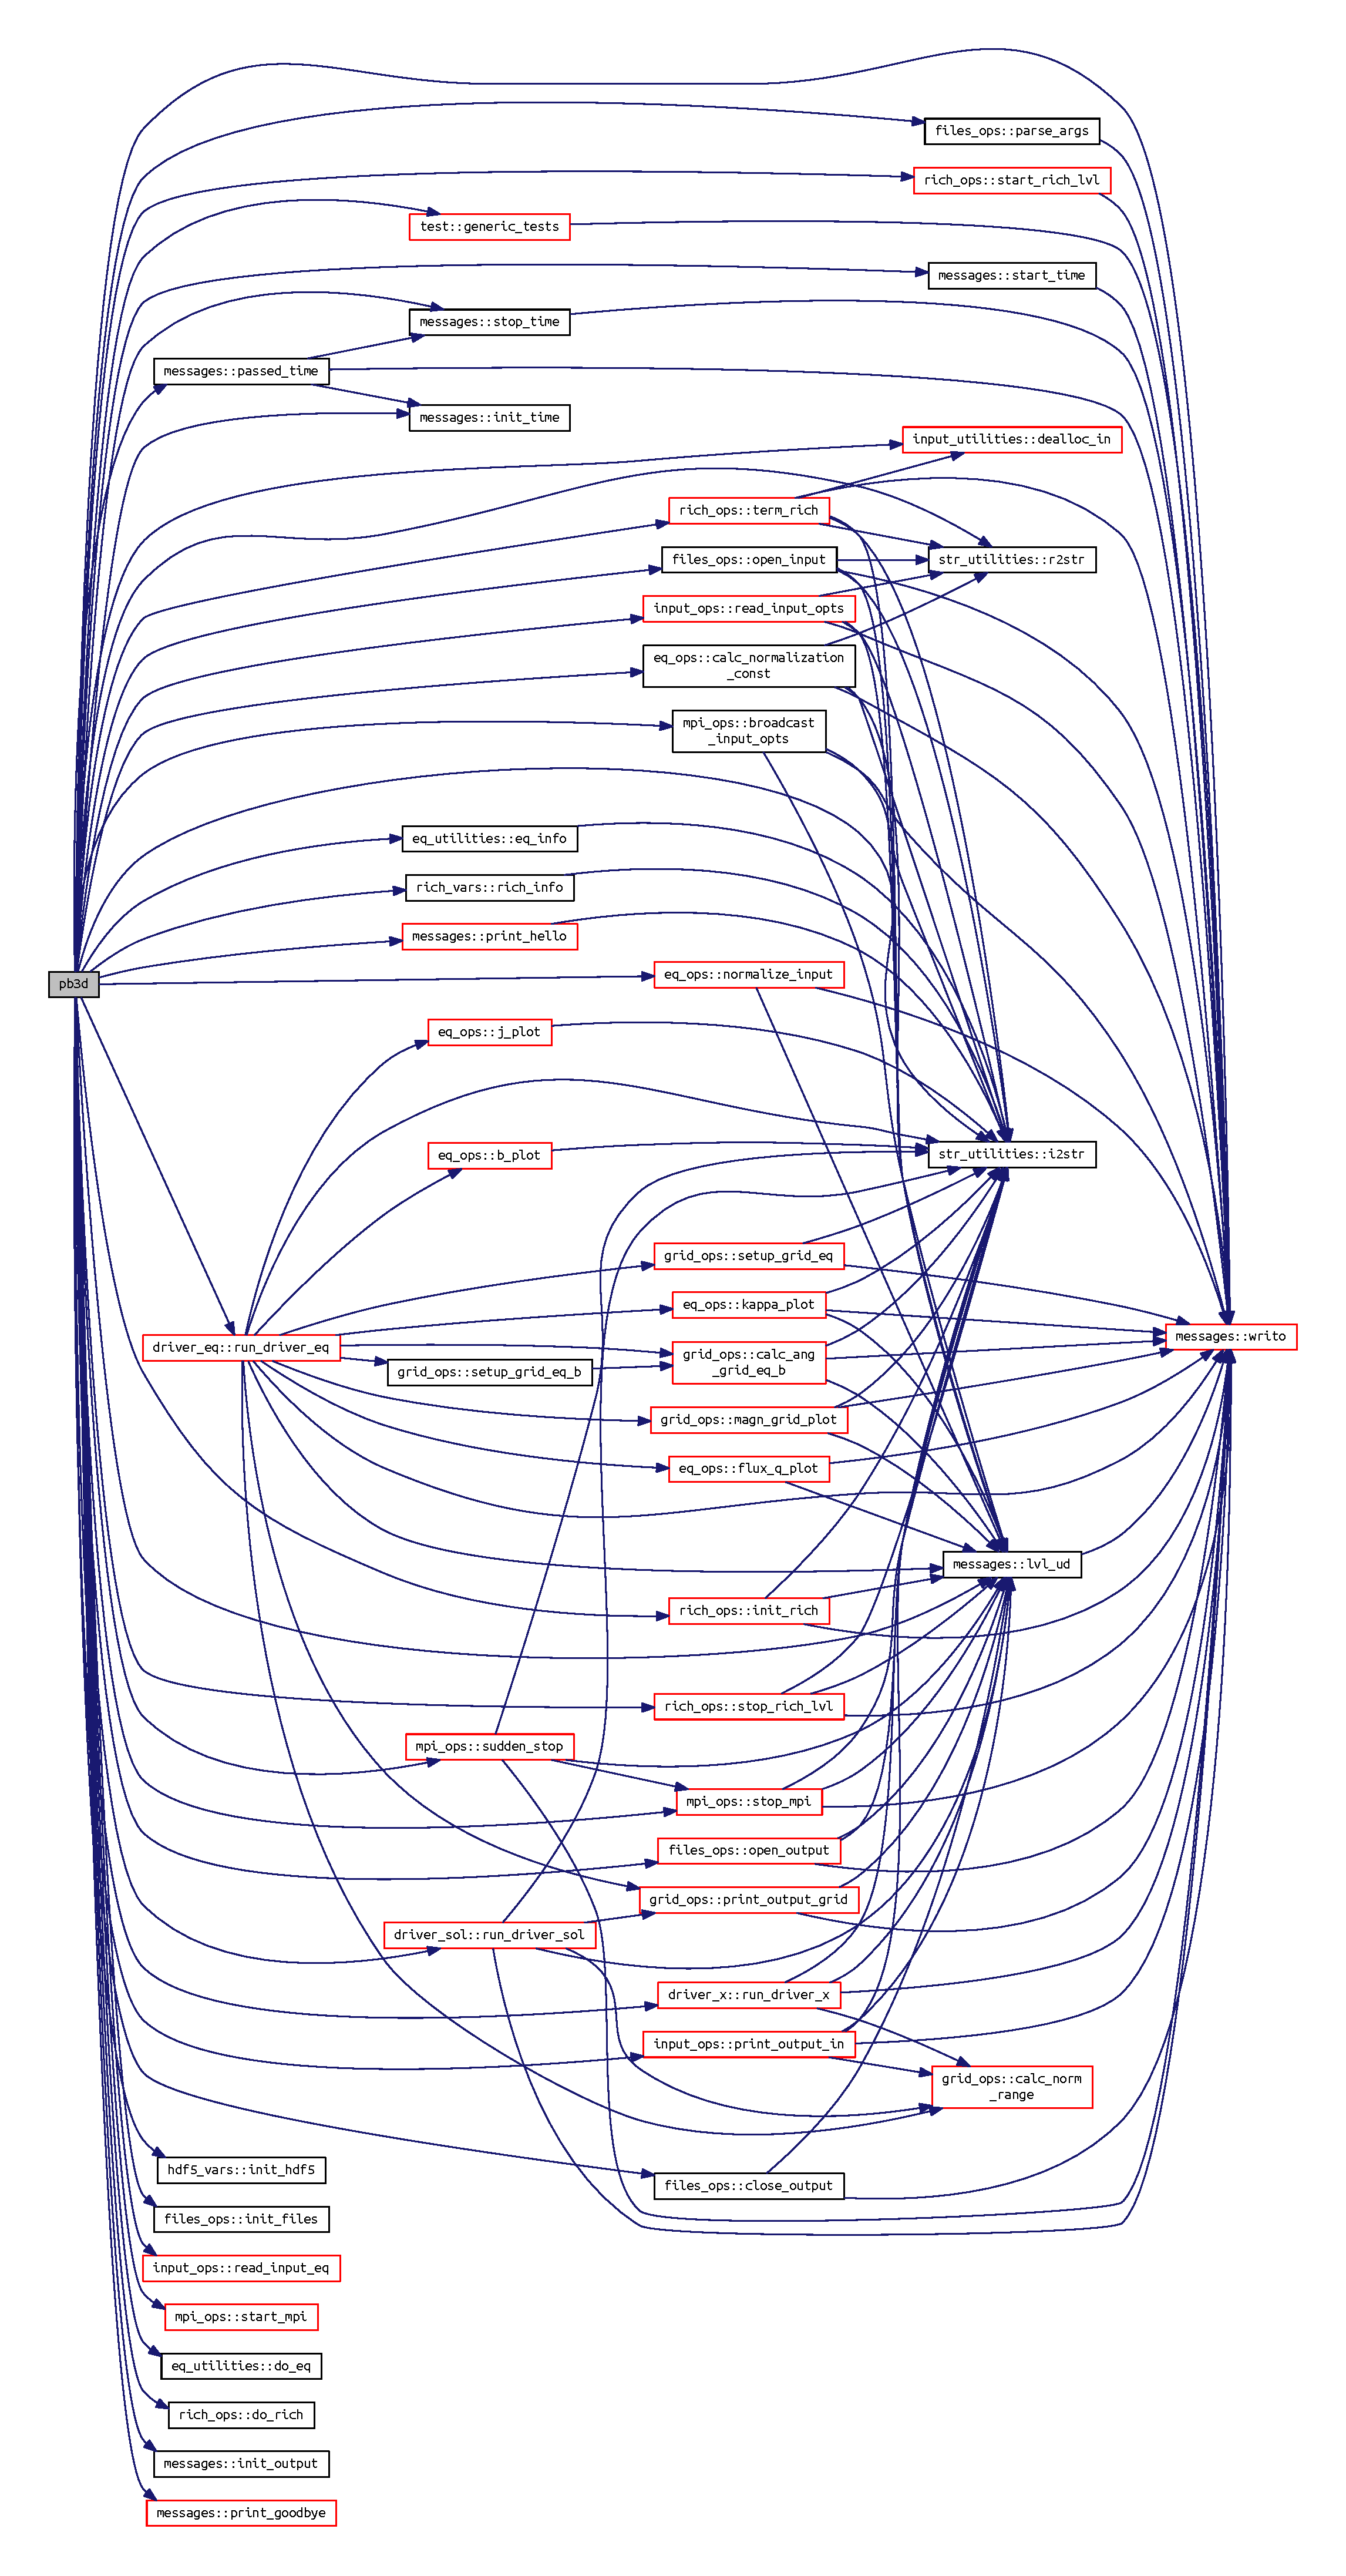
\includegraphics[height=550pt]{PB3D_8f90_afaee01f014ab3398eecac996b2795fd2_cgraph}
\end{center}
\end{figure}

\chapter{Modules}
\hypertarget{namespacedriver__eq}{}\section{driver\+\_\+eq Module Reference}
\label{namespacedriver__eq}\index{driver\+\_\+eq@{driver\+\_\+eq}}
\subsection*{Functions/\+Subroutines}
\begin{DoxyCompactItemize}
\item 
integer function, public \hyperlink{namespacedriver__eq_ac8eca434f541966edc3556d72f261eff}{run\+\_\+driver\+\_\+eq} (grid\+\_\+eq\+\_\+out, grid\+\_\+eq\+\_\+\+B\+\_\+out, eq\+\_\+1\+\_\+out, eq\+\_\+2\+\_\+out)
\end{DoxyCompactItemize}


\subsection{Function/\+Subroutine Documentation}
\mbox{\Hypertarget{namespacedriver__eq_ac8eca434f541966edc3556d72f261eff}\label{namespacedriver__eq_ac8eca434f541966edc3556d72f261eff}} 
\index{driver\+\_\+eq@{driver\+\_\+eq}!run\+\_\+driver\+\_\+eq@{run\+\_\+driver\+\_\+eq}}
\index{run\+\_\+driver\+\_\+eq@{run\+\_\+driver\+\_\+eq}!driver\+\_\+eq@{driver\+\_\+eq}}
\subsubsection{\texorpdfstring{run\+\_\+driver\+\_\+eq()}{run\_driver\_eq()}}
{\footnotesize\ttfamily integer function, public driver\+\_\+eq\+::run\+\_\+driver\+\_\+eq (\begin{DoxyParamCaption}\item[{type(grid\+\_\+type), intent(inout), target}]{grid\+\_\+eq\+\_\+out,  }\item[{type(grid\+\_\+type), intent(inout), pointer}]{grid\+\_\+eq\+\_\+\+B\+\_\+out,  }\item[{type(eq\+\_\+1\+\_\+type), intent(inout)}]{eq\+\_\+1\+\_\+out,  }\item[{type(eq\+\_\+2\+\_\+type), intent(inout)}]{eq\+\_\+2\+\_\+out }\end{DoxyParamCaption})}



Definition at line 40 of file driver\+\_\+eq.\+f90.

Here is the call graph for this function\+:
\nopagebreak
\begin{figure}[H]
\begin{center}
\leavevmode
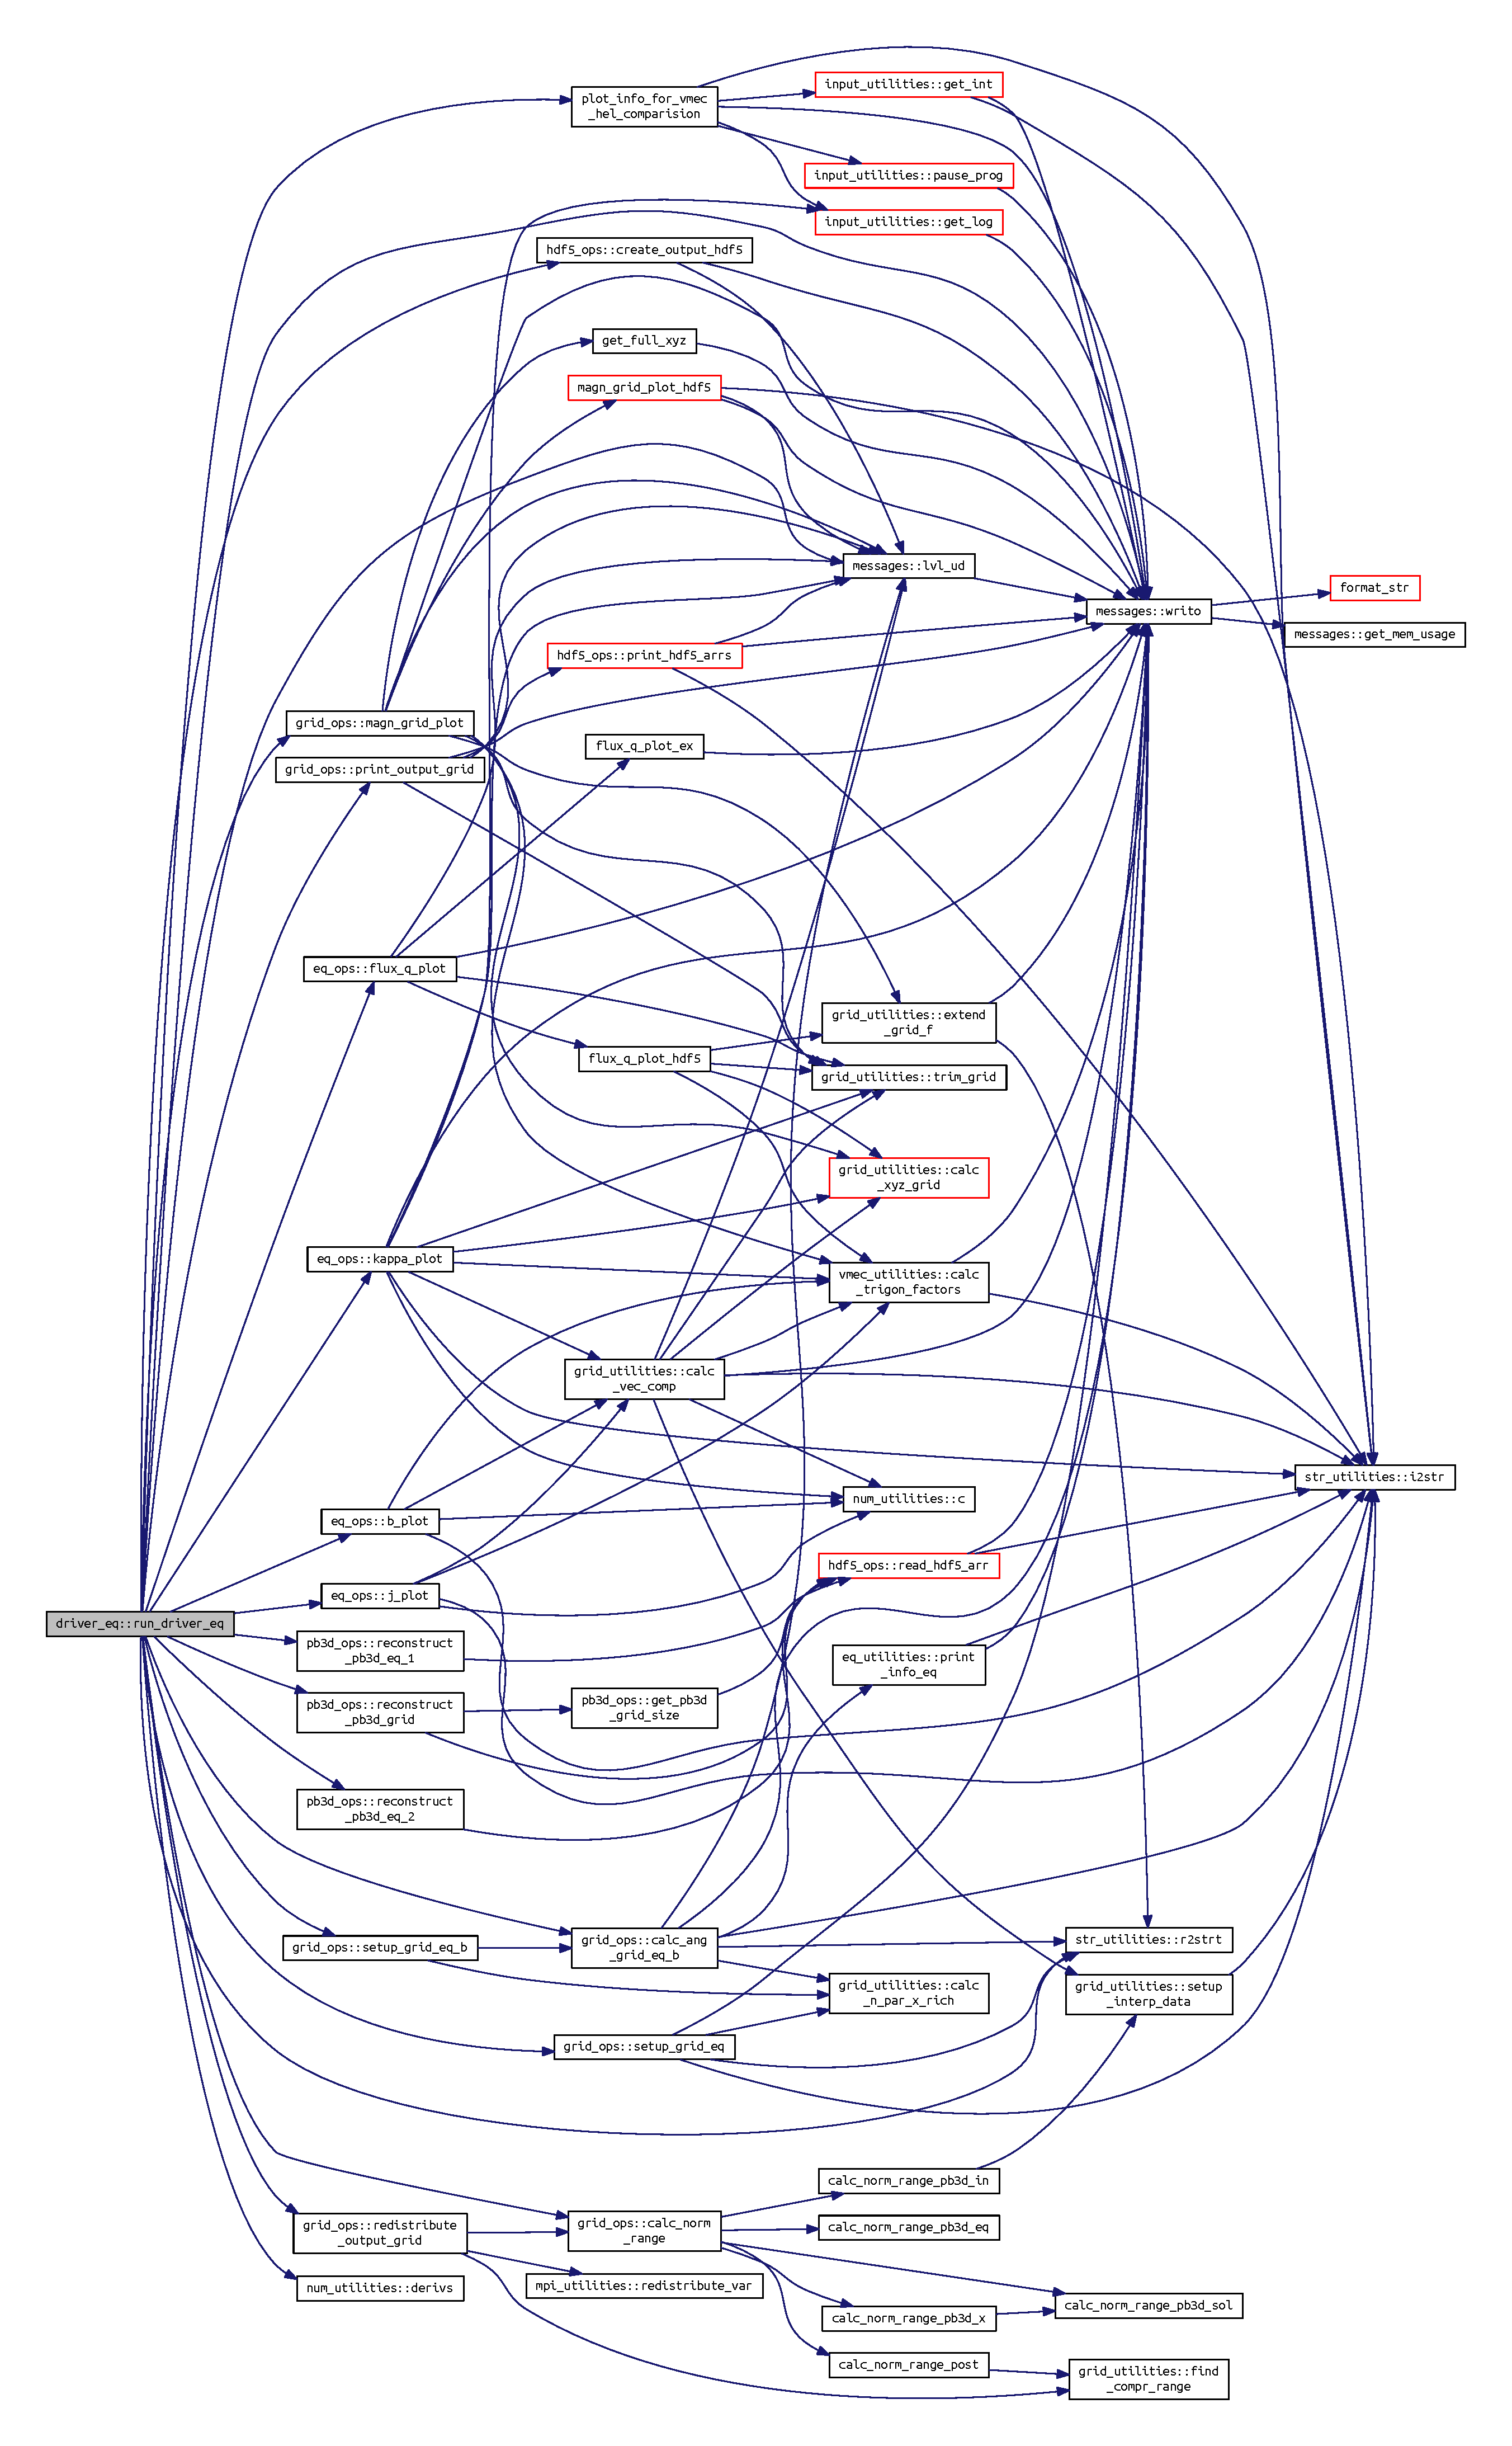
\includegraphics[height=550pt]{namespacedriver__eq_ac8eca434f541966edc3556d72f261eff_cgraph}
\end{center}
\end{figure}
Here is the caller graph for this function\+:
\nopagebreak
\begin{figure}[H]
\begin{center}
\leavevmode
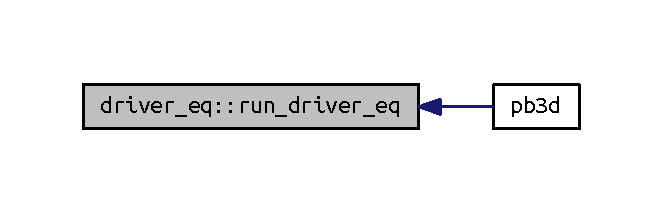
\includegraphics[width=318pt]{namespacedriver__eq_ac8eca434f541966edc3556d72f261eff_icgraph}
\end{center}
\end{figure}

\hypertarget{namespacedriver__post}{}\doxysection{driver\+\_\+post Module Reference}
\label{namespacedriver__post}\index{driver\_post@{driver\_post}}


Main driver of Post\+Processing of program Peeling Ballooning in 3D.  


\doxysubsection*{Functions/\+Subroutines}
\begin{DoxyCompactItemize}
\item 
integer function, public \mbox{\hyperlink{namespacedriver__post_af527706d4e696d4e507443d2f74194ef}{init\+\_\+post}} ()
\begin{DoxyCompactList}\small\item\em Initializes the P\+O\+ST driver. \end{DoxyCompactList}\item 
integer function, public \mbox{\hyperlink{namespacedriver__post_a33b3c6f9018a0ddc92dce77394b8ab37}{run\+\_\+driver\+\_\+post}} ()
\begin{DoxyCompactList}\small\item\em The main driver routine for postprocessing. \end{DoxyCompactList}\item 
subroutine, public \mbox{\hyperlink{namespacedriver__post_a71f9fb1935222111e1c7cfc15c5d0269}{stop\+\_\+post}} ()
\begin{DoxyCompactList}\small\item\em Cleans up main driver for postprocessing. \end{DoxyCompactList}\item 
integer function \mbox{\hyperlink{namespacedriver__post_a5d76f87f131e21b4d74fd5f4a7bbbd6b}{open\+\_\+decomp\+\_\+log}} ()
\begin{DoxyCompactList}\small\item\em Opens the decomposition log file. \end{DoxyCompactList}\item 
integer function \mbox{\hyperlink{namespacedriver__post_a4981c6c0e63b862c92ba240f43e22e77}{write\+\_\+decomp\+\_\+log}} (X\+\_\+id, E\+\_\+pot\+\_\+int, E\+\_\+kin\+\_\+int)
\begin{DoxyCompactList}\small\item\em Write to decomposition log file. \end{DoxyCompactList}\item 
subroutine \mbox{\hyperlink{namespacedriver__post_a51ecad1032e415d2a8e6e5b97d2c7e09}{find\+\_\+stab\+\_\+ranges}} (sol, min\+\_\+id, max\+\_\+id, last\+\_\+unstable\+\_\+id)
\begin{DoxyCompactList}\small\item\em finds the plot ranges {\ttfamily min\+\_\+id} and {\ttfamily max\+\_\+id}. \end{DoxyCompactList}\item 
subroutine \mbox{\hyperlink{namespacedriver__post_af9ce961d2d6825b767a93fdbe8806a1c}{plot\+\_\+sol\+\_\+val\+\_\+comp}} (sol\+\_\+val\+\_\+comp)
\begin{DoxyCompactList}\small\item\em Plots difference between Eigenvalues and energy fraction. \end{DoxyCompactList}\item 
integer function \mbox{\hyperlink{namespacedriver__post_a3438685c5fb7302f756c368fb5f940ee}{setup\+\_\+out\+\_\+grids}} (grids\+\_\+out, X\+Y\+Z\+\_\+eq, X\+Y\+Z\+\_\+sol)
\begin{DoxyCompactList}\small\item\em Sets up the output grids for a particular parallel job. \end{DoxyCompactList}\end{DoxyCompactItemize}


\doxysubsection{Detailed Description}
Main driver of Post\+Processing of program Peeling Ballooning in 3D. 

\doxysubsection{Function/\+Subroutine Documentation}
\mbox{\Hypertarget{namespacedriver__post_a51ecad1032e415d2a8e6e5b97d2c7e09}\label{namespacedriver__post_a51ecad1032e415d2a8e6e5b97d2c7e09}} 
\index{driver\_post@{driver\_post}!find\_stab\_ranges@{find\_stab\_ranges}}
\index{find\_stab\_ranges@{find\_stab\_ranges}!driver\_post@{driver\_post}}
\doxysubsubsection{\texorpdfstring{find\_stab\_ranges()}{find\_stab\_ranges()}}
{\footnotesize\ttfamily subroutine driver\+\_\+post\+::find\+\_\+stab\+\_\+ranges (\begin{DoxyParamCaption}\item[{type(\mbox{\hyperlink{structsol__vars_1_1sol__type}{sol\+\_\+type}}), intent(in)}]{sol,  }\item[{integer, dimension(3), intent(inout)}]{min\+\_\+id,  }\item[{integer, dimension(3), intent(inout)}]{max\+\_\+id,  }\item[{integer, intent(inout)}]{last\+\_\+unstable\+\_\+id }\end{DoxyParamCaption})}



finds the plot ranges {\ttfamily min\+\_\+id} and {\ttfamily max\+\_\+id}. 

There are three ranges, calculated using n\+\_\+sol\+\_\+plotted, which indicates\+:
\begin{DoxyEnumerate}
\item how many of the first EV\textquotesingle{}s in the unstable range
\item how many of the last EV\textquotesingle{}s in the unstable range
\item how many of the first EV\textquotesingle{}s in the stable range
\item how many of the last EV\textquotesingle{}s in the stable range
\end{DoxyEnumerate}

have to be plotted.

This yields maximally three different ranges\+: One starting at the first unstable EV, one centered around the zero of the EV\textquotesingle{}s and one ending at the last EV. These ranges can be disjoint but do not have to be.~\newline
 Also, it is possible that a range does not exist, for example if there are no unstable EV\textquotesingle{}s.

\begin{DoxyNote}{Note}
A negative value for the elements in n\+\_\+sol\+\_\+plotted means \char`\"{}all
 values in range\char`\"{}\+:
\begin{DoxyEnumerate}
\item or 2. full unstable range
\item or 4. full stable range 
\end{DoxyEnumerate}
\end{DoxyNote}

\begin{DoxyParams}[1]{Parameters}
\mbox{\texttt{ in}}  & {\em sol} & solution variables \\
\hline
\mbox{\texttt{ in,out}}  & {\em min\+\_\+id} & min. index of range 1, 2 and 3 \\
\hline
\mbox{\texttt{ in,out}}  & {\em max\+\_\+id} & max. index of range 1, 2 and 3 \\
\hline
\mbox{\texttt{ in,out}}  & {\em last\+\_\+unstable\+\_\+id} & index of last unstable EV \\
\hline
\end{DoxyParams}


Definition at line 1037 of file driver\+\_\+\+P\+O\+S\+T.\+f90.

Here is the caller graph for this function\+:\nopagebreak
\begin{figure}[H]
\begin{center}
\leavevmode
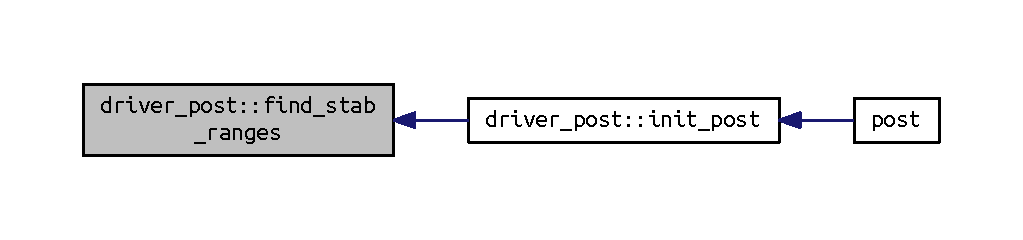
\includegraphics[width=350pt]{namespacedriver__post_a51ecad1032e415d2a8e6e5b97d2c7e09_icgraph}
\end{center}
\end{figure}
\mbox{\Hypertarget{namespacedriver__post_af527706d4e696d4e507443d2f74194ef}\label{namespacedriver__post_af527706d4e696d4e507443d2f74194ef}} 
\index{driver\_post@{driver\_post}!init\_post@{init\_post}}
\index{init\_post@{init\_post}!driver\_post@{driver\_post}}
\doxysubsubsection{\texorpdfstring{init\_post()}{init\_post()}}
{\footnotesize\ttfamily integer function, public driver\+\_\+post\+::init\+\_\+post}



Initializes the P\+O\+ST driver. 


\begin{DoxyItemize}
\item set up preliminary variables
\begin{DoxyItemize}
\item global variables
\item read grids (full)
\item {\ttfamily eq\+\_\+1} (full) and {\ttfamily n} \& {\ttfamily m} (full)
\end{DoxyItemize}
\item set up output grids\+:
\begin{DoxyItemize}
\item {\ttfamily  P\+O\+S\+T\+\_\+style = 1}\+: extended grid
\item {\ttfamily  P\+O\+S\+T\+\_\+style = 2}\+: field-\/aligned grid
\end{DoxyItemize}
\item clean up
\item set up final variables
\begin{DoxyItemize}
\item normal limits
\item read grids (divided), {\ttfamily eq\+\_\+1} (divided) and {\ttfamily sol} (divided) variables
\end{DoxyItemize}
\item 1-\/D output plots
\begin{DoxyItemize}
\item resonance plot
\item flux quantities plot
\item magnetic grid plot
\end{DoxyItemize}
\item prepare Eigenvalue plots
\begin{DoxyItemize}
\item calculates resonant surfaces
\item plots Eigenvalues
\item finds stability ranges for all Eigenvalues to be plot
\item plots harmonics for every Eigenvalue
\item calculates the parallel ranges of the equilibrium jobs
\end{DoxyItemize}
\item clean up
\end{DoxyItemize}

In the actual driver, more detailed plots are possibly made for all requested Eigenvalues if {\ttfamily full\+\_\+output}.

\begin{DoxyReturn}{Returns}
ierr 
\end{DoxyReturn}


Definition at line 77 of file driver\+\_\+\+P\+O\+S\+T.\+f90.

Here is the call graph for this function\+:\nopagebreak
\begin{figure}[H]
\begin{center}
\leavevmode
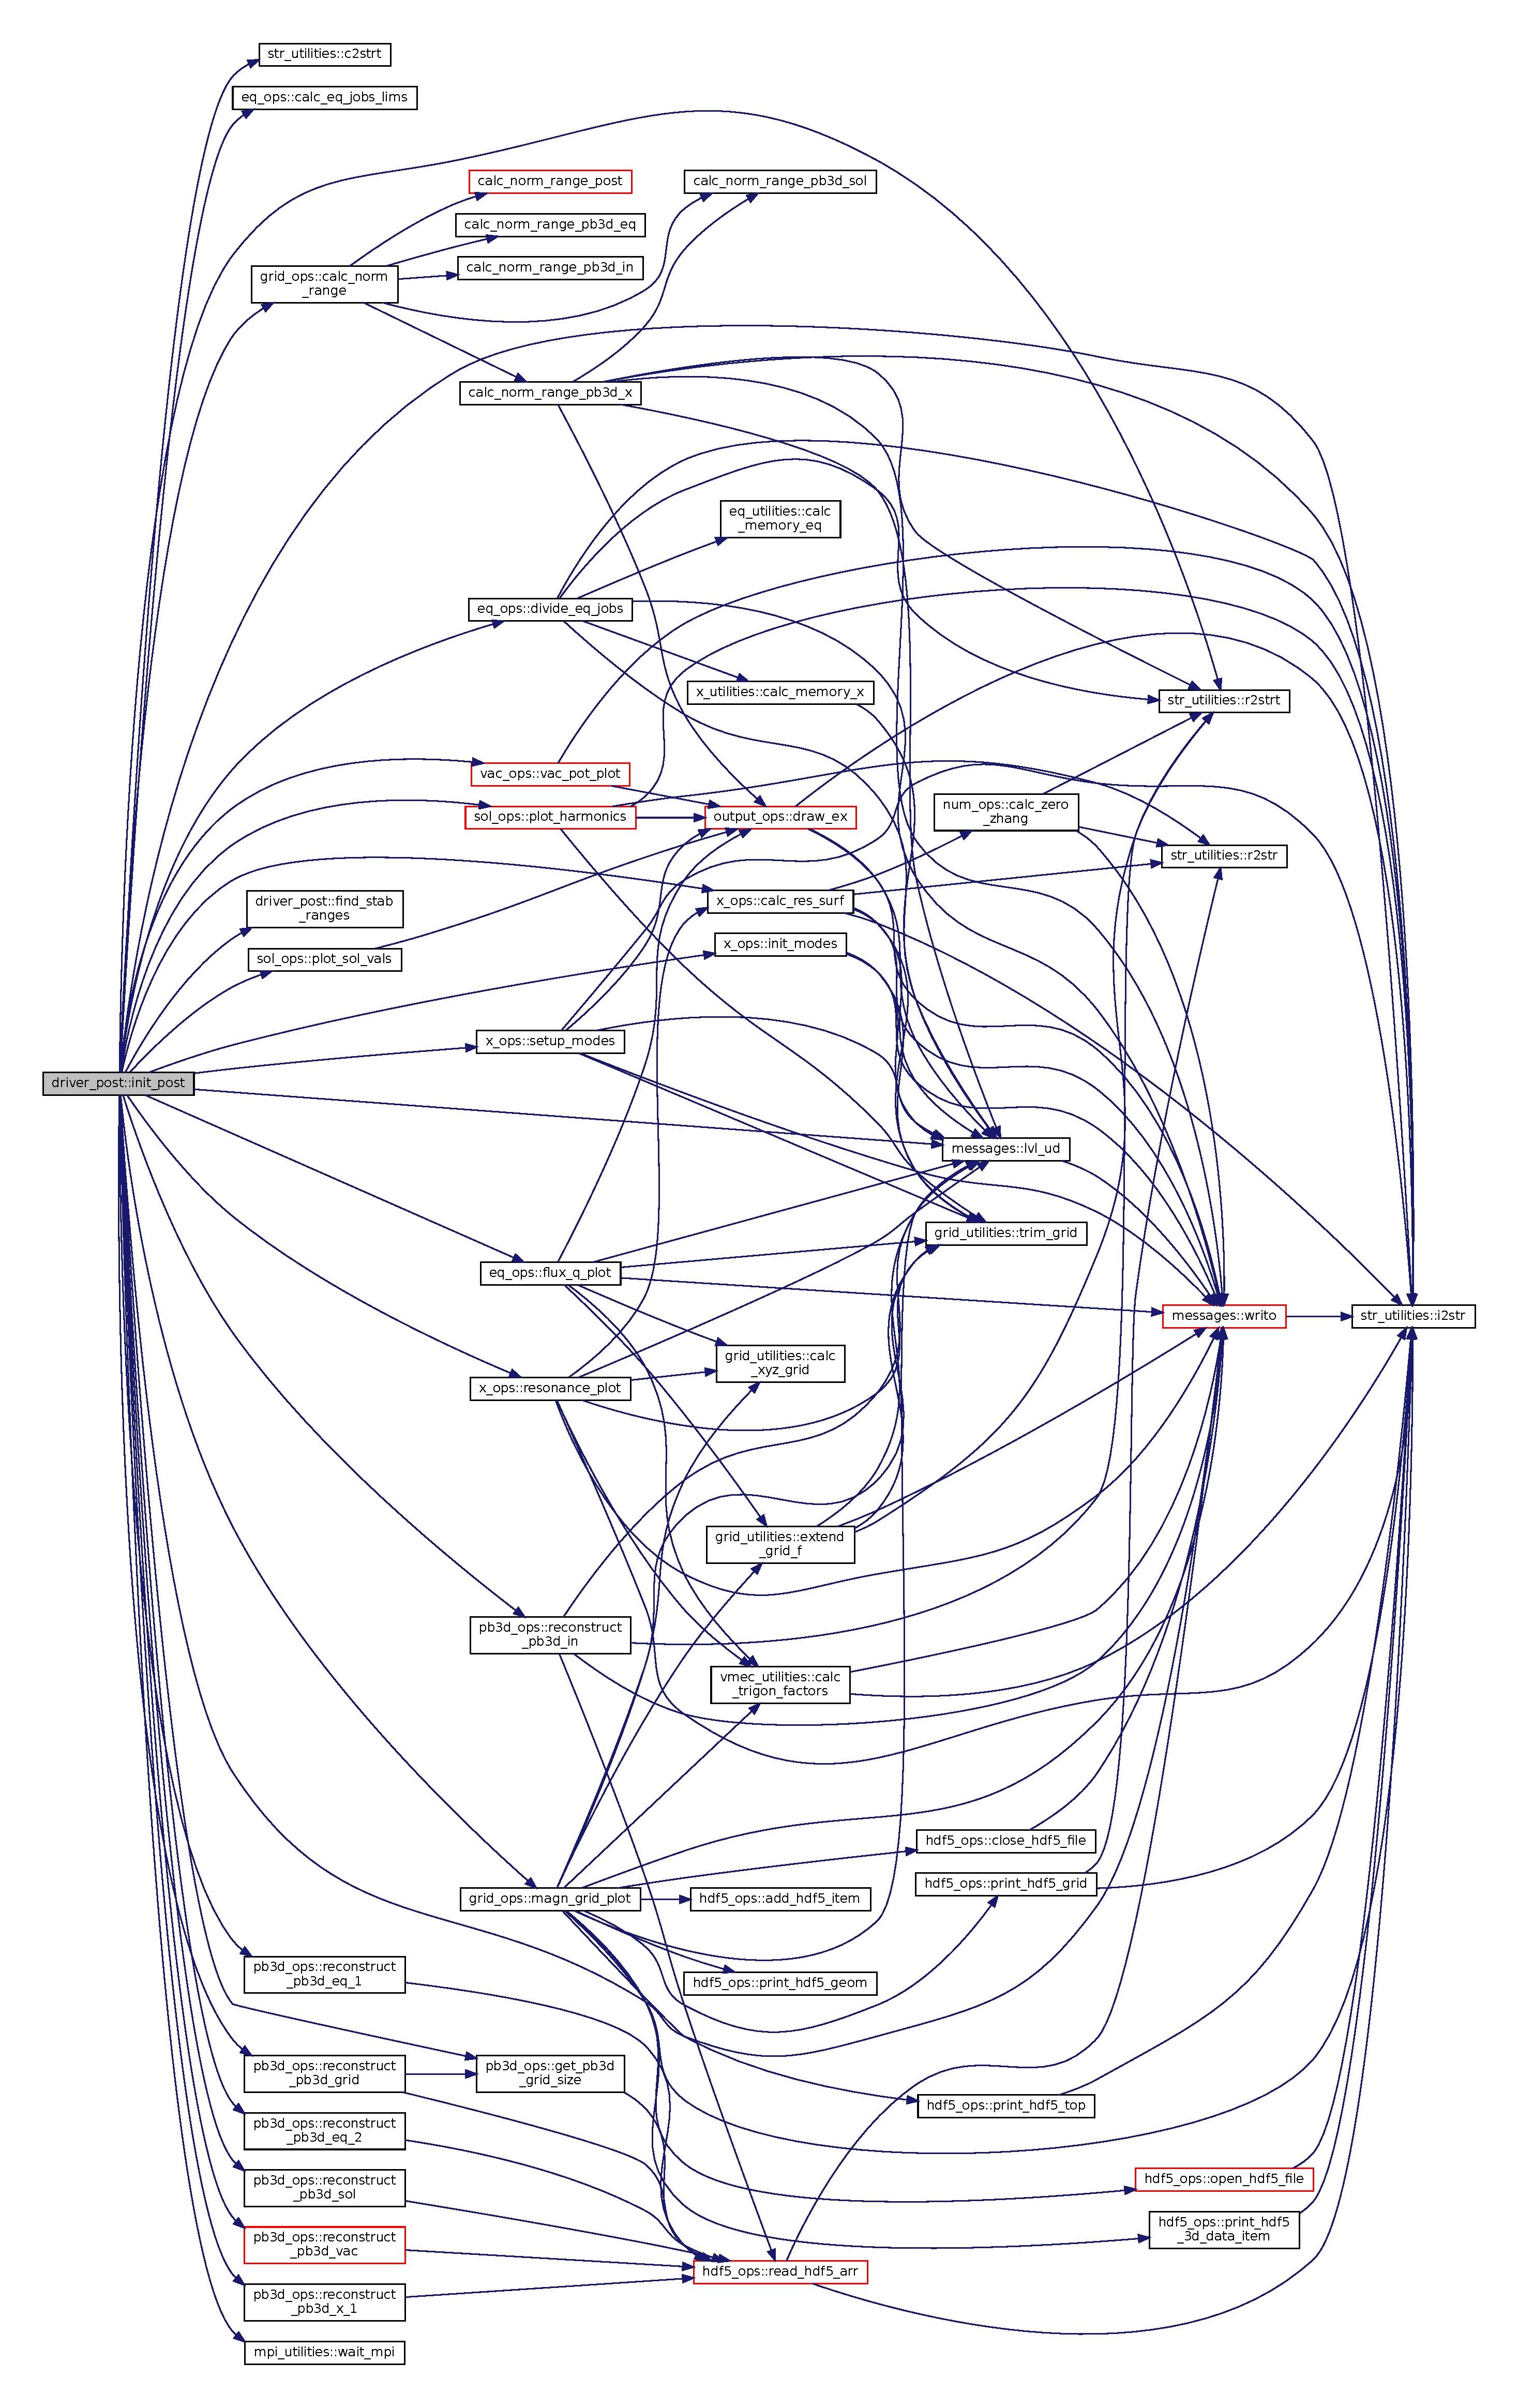
\includegraphics[height=550pt]{namespacedriver__post_af527706d4e696d4e507443d2f74194ef_cgraph}
\end{center}
\end{figure}
Here is the caller graph for this function\+:\nopagebreak
\begin{figure}[H]
\begin{center}
\leavevmode
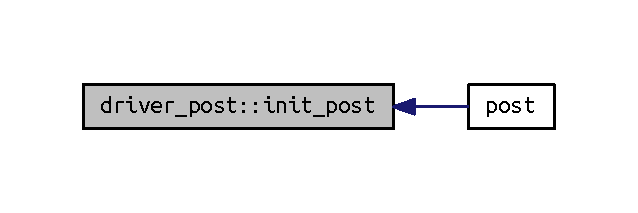
\includegraphics[width=298pt]{namespacedriver__post_af527706d4e696d4e507443d2f74194ef_icgraph}
\end{center}
\end{figure}
\mbox{\Hypertarget{namespacedriver__post_a5d76f87f131e21b4d74fd5f4a7bbbd6b}\label{namespacedriver__post_a5d76f87f131e21b4d74fd5f4a7bbbd6b}} 
\index{driver\_post@{driver\_post}!open\_decomp\_log@{open\_decomp\_log}}
\index{open\_decomp\_log@{open\_decomp\_log}!driver\_post@{driver\_post}}
\doxysubsubsection{\texorpdfstring{open\_decomp\_log()}{open\_decomp\_log()}}
{\footnotesize\ttfamily integer function driver\+\_\+post\+::open\+\_\+decomp\+\_\+log}



Opens the decomposition log file. 

\begin{DoxyReturn}{Returns}
ierr 
\end{DoxyReturn}


Definition at line 841 of file driver\+\_\+\+P\+O\+S\+T.\+f90.

Here is the call graph for this function\+:\nopagebreak
\begin{figure}[H]
\begin{center}
\leavevmode
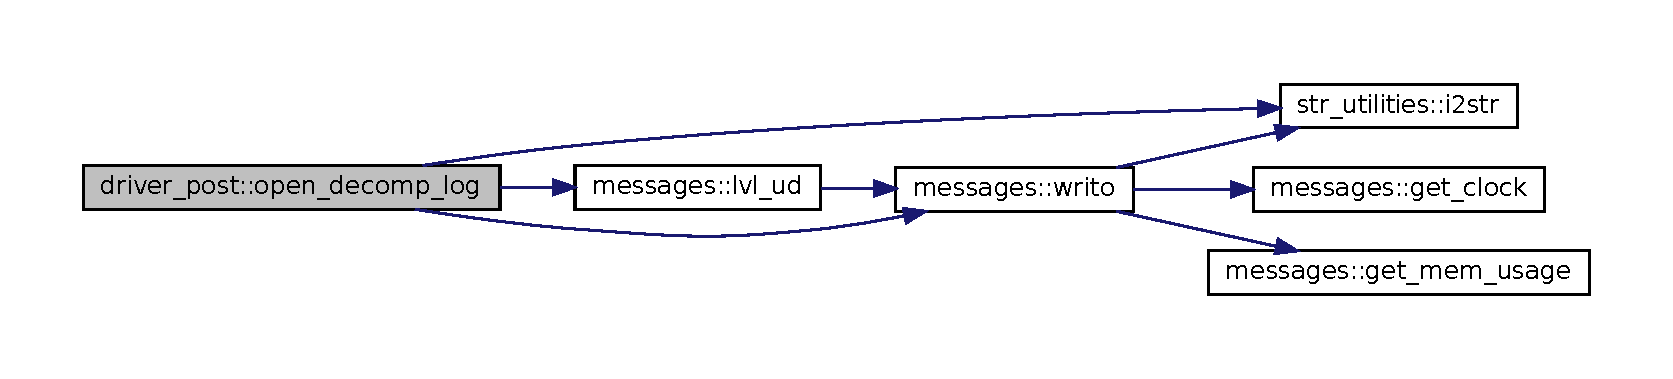
\includegraphics[width=350pt]{namespacedriver__post_a5d76f87f131e21b4d74fd5f4a7bbbd6b_cgraph}
\end{center}
\end{figure}
Here is the caller graph for this function\+:\nopagebreak
\begin{figure}[H]
\begin{center}
\leavevmode
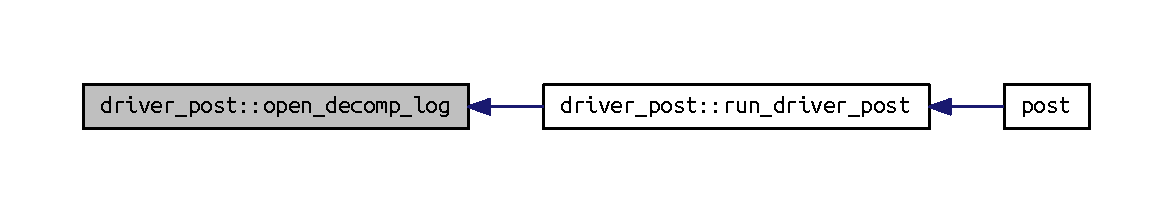
\includegraphics[width=350pt]{namespacedriver__post_a5d76f87f131e21b4d74fd5f4a7bbbd6b_icgraph}
\end{center}
\end{figure}
\mbox{\Hypertarget{namespacedriver__post_af9ce961d2d6825b767a93fdbe8806a1c}\label{namespacedriver__post_af9ce961d2d6825b767a93fdbe8806a1c}} 
\index{driver\_post@{driver\_post}!plot\_sol\_val\_comp@{plot\_sol\_val\_comp}}
\index{plot\_sol\_val\_comp@{plot\_sol\_val\_comp}!driver\_post@{driver\_post}}
\doxysubsubsection{\texorpdfstring{plot\_sol\_val\_comp()}{plot\_sol\_val\_comp()}}
{\footnotesize\ttfamily subroutine driver\+\_\+post\+::plot\+\_\+sol\+\_\+val\+\_\+comp (\begin{DoxyParamCaption}\item[{complex(dp), dimension(\+:,\+:,\+:), intent(inout)}]{sol\+\_\+val\+\_\+comp }\end{DoxyParamCaption})}



Plots difference between Eigenvalues and energy fraction. 


\begin{DoxyParams}[1]{Parameters}
\mbox{\texttt{ in,out}}  & {\em sol\+\_\+val\+\_\+comp} & fraction between total $E_{\text{pot}}$ and $E_{\text{kin}}$, compared with EV \\
\hline
\end{DoxyParams}


Definition at line 1113 of file driver\+\_\+\+P\+O\+S\+T.\+f90.

Here is the call graph for this function\+:\nopagebreak
\begin{figure}[H]
\begin{center}
\leavevmode
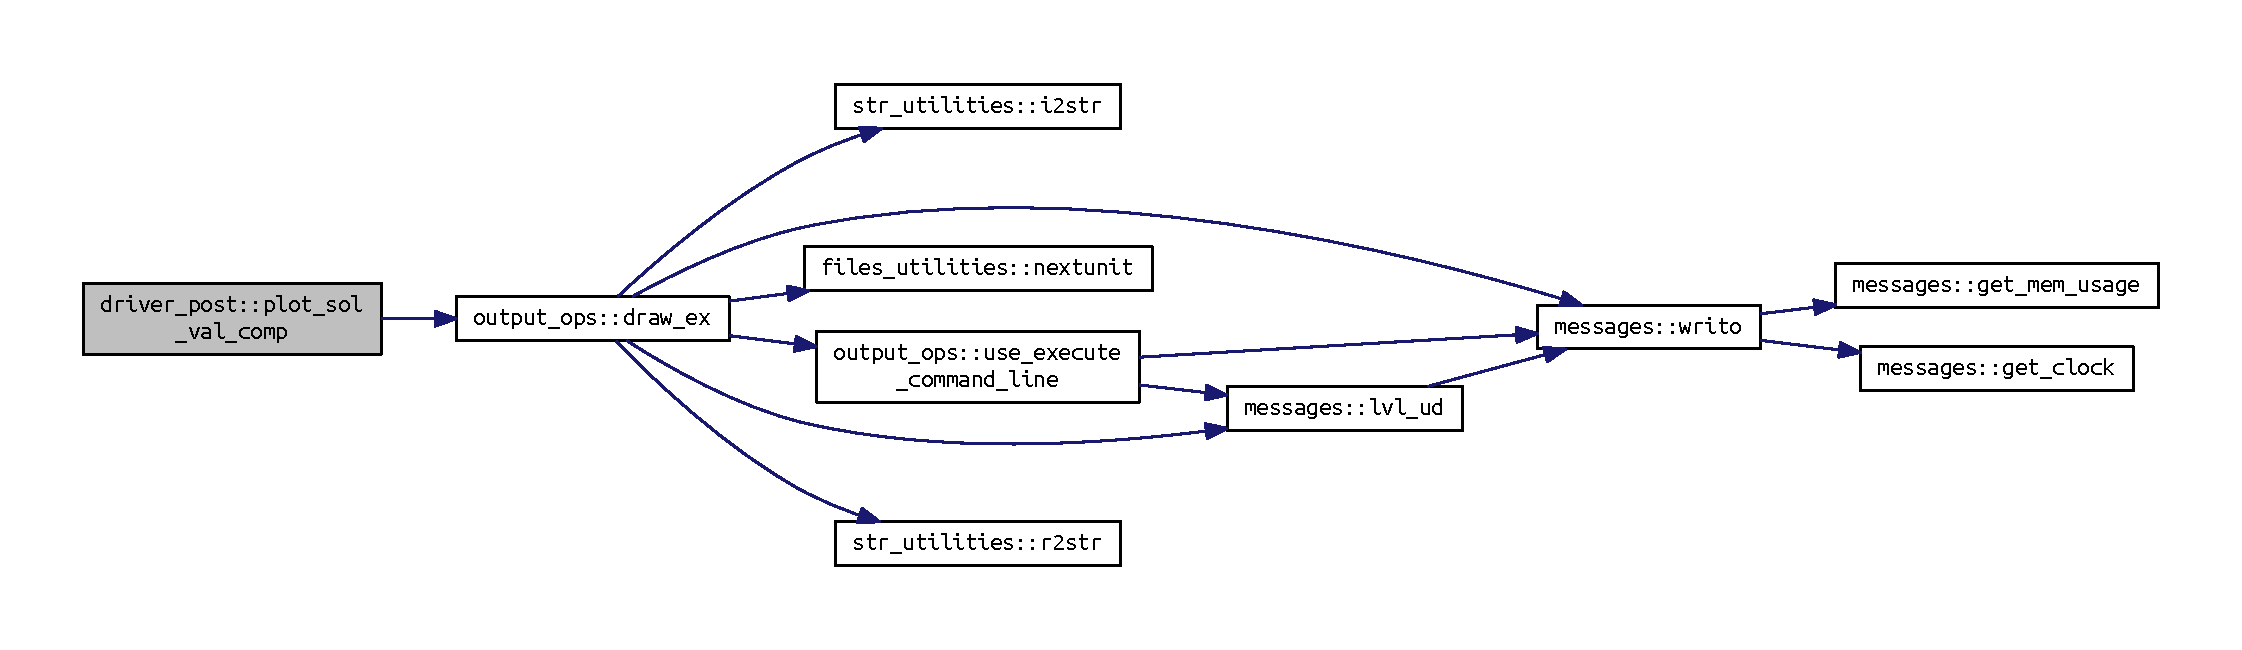
\includegraphics[width=350pt]{namespacedriver__post_af9ce961d2d6825b767a93fdbe8806a1c_cgraph}
\end{center}
\end{figure}
Here is the caller graph for this function\+:\nopagebreak
\begin{figure}[H]
\begin{center}
\leavevmode
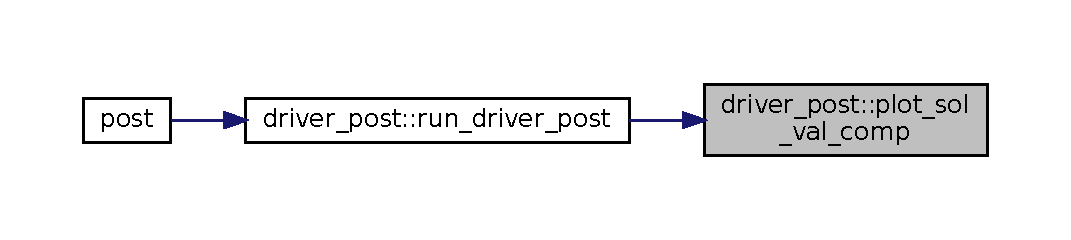
\includegraphics[width=350pt]{namespacedriver__post_af9ce961d2d6825b767a93fdbe8806a1c_icgraph}
\end{center}
\end{figure}
\mbox{\Hypertarget{namespacedriver__post_a33b3c6f9018a0ddc92dce77394b8ab37}\label{namespacedriver__post_a33b3c6f9018a0ddc92dce77394b8ab37}} 
\index{driver\_post@{driver\_post}!run\_driver\_post@{run\_driver\_post}}
\index{run\_driver\_post@{run\_driver\_post}!driver\_post@{driver\_post}}
\doxysubsubsection{\texorpdfstring{run\_driver\_post()}{run\_driver\_post()}}
{\footnotesize\ttfamily integer function, public driver\+\_\+post\+::run\+\_\+driver\+\_\+post}



The main driver routine for postprocessing. 

\begin{DoxyNote}{Note}
The P\+B3D output is given on different grids for different styles of the equilibrium model\+:
\begin{DoxyItemize}
\item V\+M\+EC\+: field-\/aligned grid on which EV problem has been solved.
\item H\+E\+L\+E\+NA\+: output grid on which equilibrium and metric variables are tabulated.
\end{DoxyItemize}
\end{DoxyNote}
Furthermore, if Richardson extrapolation is used, the V\+M\+EC grids and variables are contained in multiple H\+D\+F5 variables. These variables are needed here both in a field-\/aligned and a plot grid.

A consequence of the above is that for V\+M\+EC the field-\/aligned output is already given, but the output on the plot grid has to be calculated from scratch, while for H\+E\+L\+E\+NA both outputs have to be interpolated from the output tables.

The general workflow is as follows\+:
\begin{DoxyItemize}
\item take a subset of the output grids for the current equilibrium job.
\item for {\ttfamily P\+O\+S\+T\+\_\+style = 1} (extended grid)\+:
\begin{DoxyItemize}
\item V\+M\+EC\+: recalculate variables
\item H\+EL\+: interpolate variables for {\ttfamily P\+O\+S\+T\+\_\+style = 2} (B-\/aligned grid)\+:
\item V\+M\+EC\+: read subset of variables
\item H\+EL\+: interpolate variables
\end{DoxyItemize}
\item create helper variables
\item create plots and outputs
\end{DoxyItemize}

\begin{DoxyReturn}{Returns}
ierr 
\end{DoxyReturn}


Definition at line 542 of file driver\+\_\+\+P\+O\+S\+T.\+f90.

Here is the call graph for this function\+:\nopagebreak
\begin{figure}[H]
\begin{center}
\leavevmode
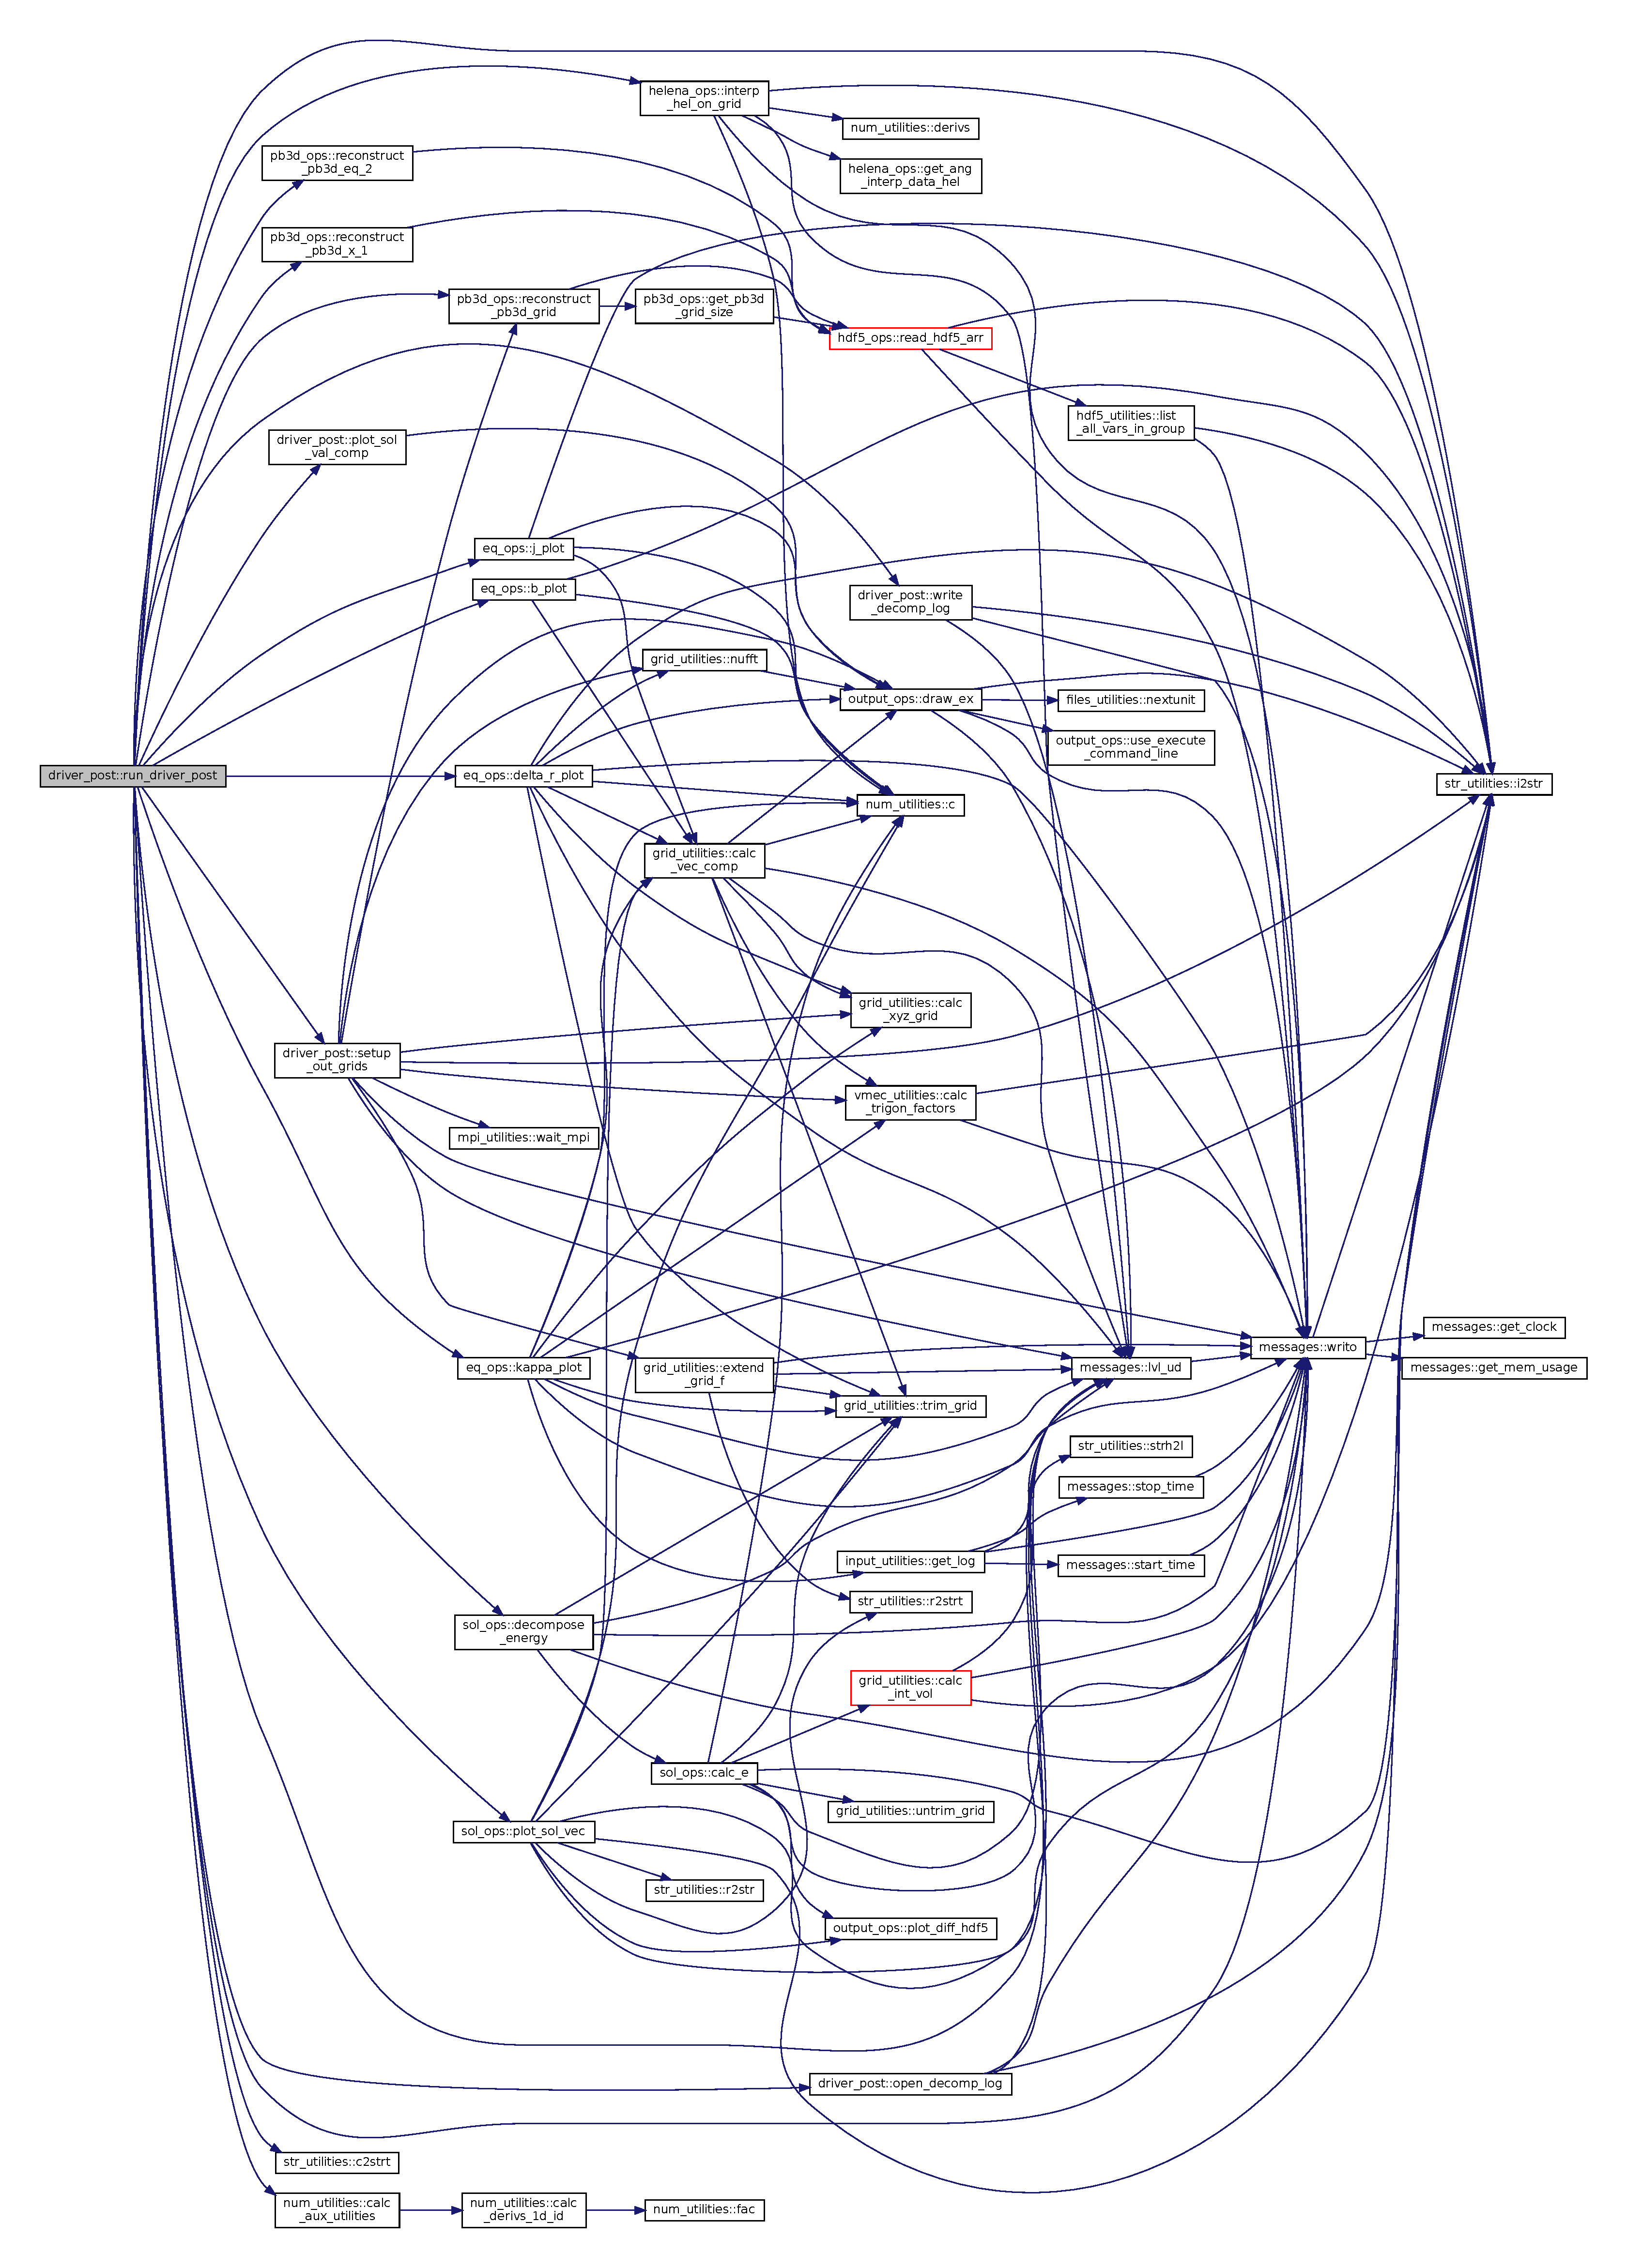
\includegraphics[width=350pt]{namespacedriver__post_a33b3c6f9018a0ddc92dce77394b8ab37_cgraph}
\end{center}
\end{figure}
Here is the caller graph for this function\+:\nopagebreak
\begin{figure}[H]
\begin{center}
\leavevmode
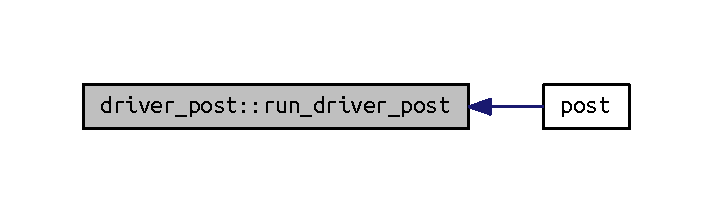
\includegraphics[width=342pt]{namespacedriver__post_a33b3c6f9018a0ddc92dce77394b8ab37_icgraph}
\end{center}
\end{figure}
\mbox{\Hypertarget{namespacedriver__post_a3438685c5fb7302f756c368fb5f940ee}\label{namespacedriver__post_a3438685c5fb7302f756c368fb5f940ee}} 
\index{driver\_post@{driver\_post}!setup\_out\_grids@{setup\_out\_grids}}
\index{setup\_out\_grids@{setup\_out\_grids}!driver\_post@{driver\_post}}
\doxysubsubsection{\texorpdfstring{setup\_out\_grids()}{setup\_out\_grids()}}
{\footnotesize\ttfamily integer function driver\+\_\+post\+::setup\+\_\+out\+\_\+grids (\begin{DoxyParamCaption}\item[{type(\mbox{\hyperlink{structgrid__vars_1_1grid__type}{grid\+\_\+type}}), dimension(3), intent(inout)}]{grids\+\_\+out,  }\item[{real(dp), dimension(\+:,\+:,\+:,\+:), intent(inout), allocatable}]{X\+Y\+Z\+\_\+eq,  }\item[{real(dp), dimension(\+:,\+:,\+:,\+:), intent(inout), allocatable}]{X\+Y\+Z\+\_\+sol }\end{DoxyParamCaption})}



Sets up the output grids for a particular parallel job. 

Three grids are returned\+:
\begin{DoxyItemize}
\item eq
\item X
\item sol
\end{DoxyItemize}

The normal coordinates of these grids correspond to the one used in P\+B3D. For X this is determined by {\ttfamily x\+\_\+grid\+\_\+style}.

The angular components of the eq and X grids is determined by {\ttfamily post\+\_\+style\+:} 
\begin{DoxyItemize}
\item 1\+: extended grid with {\ttfamily min\+\_\+theta\+\_\+plot}, {\ttfamily max\+\_\+theta\+\_\+plot}, {\ttfamily min\+\_\+zeta\+\_\+plot} and {\ttfamily max\+\_\+zeta\+\_\+plot}.
\item 2\+: P\+B3D grid.
\end{DoxyItemize}

\begin{DoxyReturn}{Returns}
ierr 
\end{DoxyReturn}

\begin{DoxyParams}[1]{Parameters}
\mbox{\texttt{ in,out}}  & {\em grids\+\_\+out} & eq, X and sol output grids (full parallel and normal range) \\
\hline
\mbox{\texttt{ in,out}}  & {\em xyz\+\_\+eq} & {\ttfamily X}, {\ttfamily Y} and {\ttfamily Z} on output equilibrium grid \\
\hline
\mbox{\texttt{ in,out}}  & {\em xyz\+\_\+sol} & {\ttfamily X}, {\ttfamily Y} and {\ttfamily Z} on output solution grid \\
\hline
\end{DoxyParams}


Definition at line 1186 of file driver\+\_\+\+P\+O\+S\+T.\+f90.

Here is the call graph for this function\+:\nopagebreak
\begin{figure}[H]
\begin{center}
\leavevmode
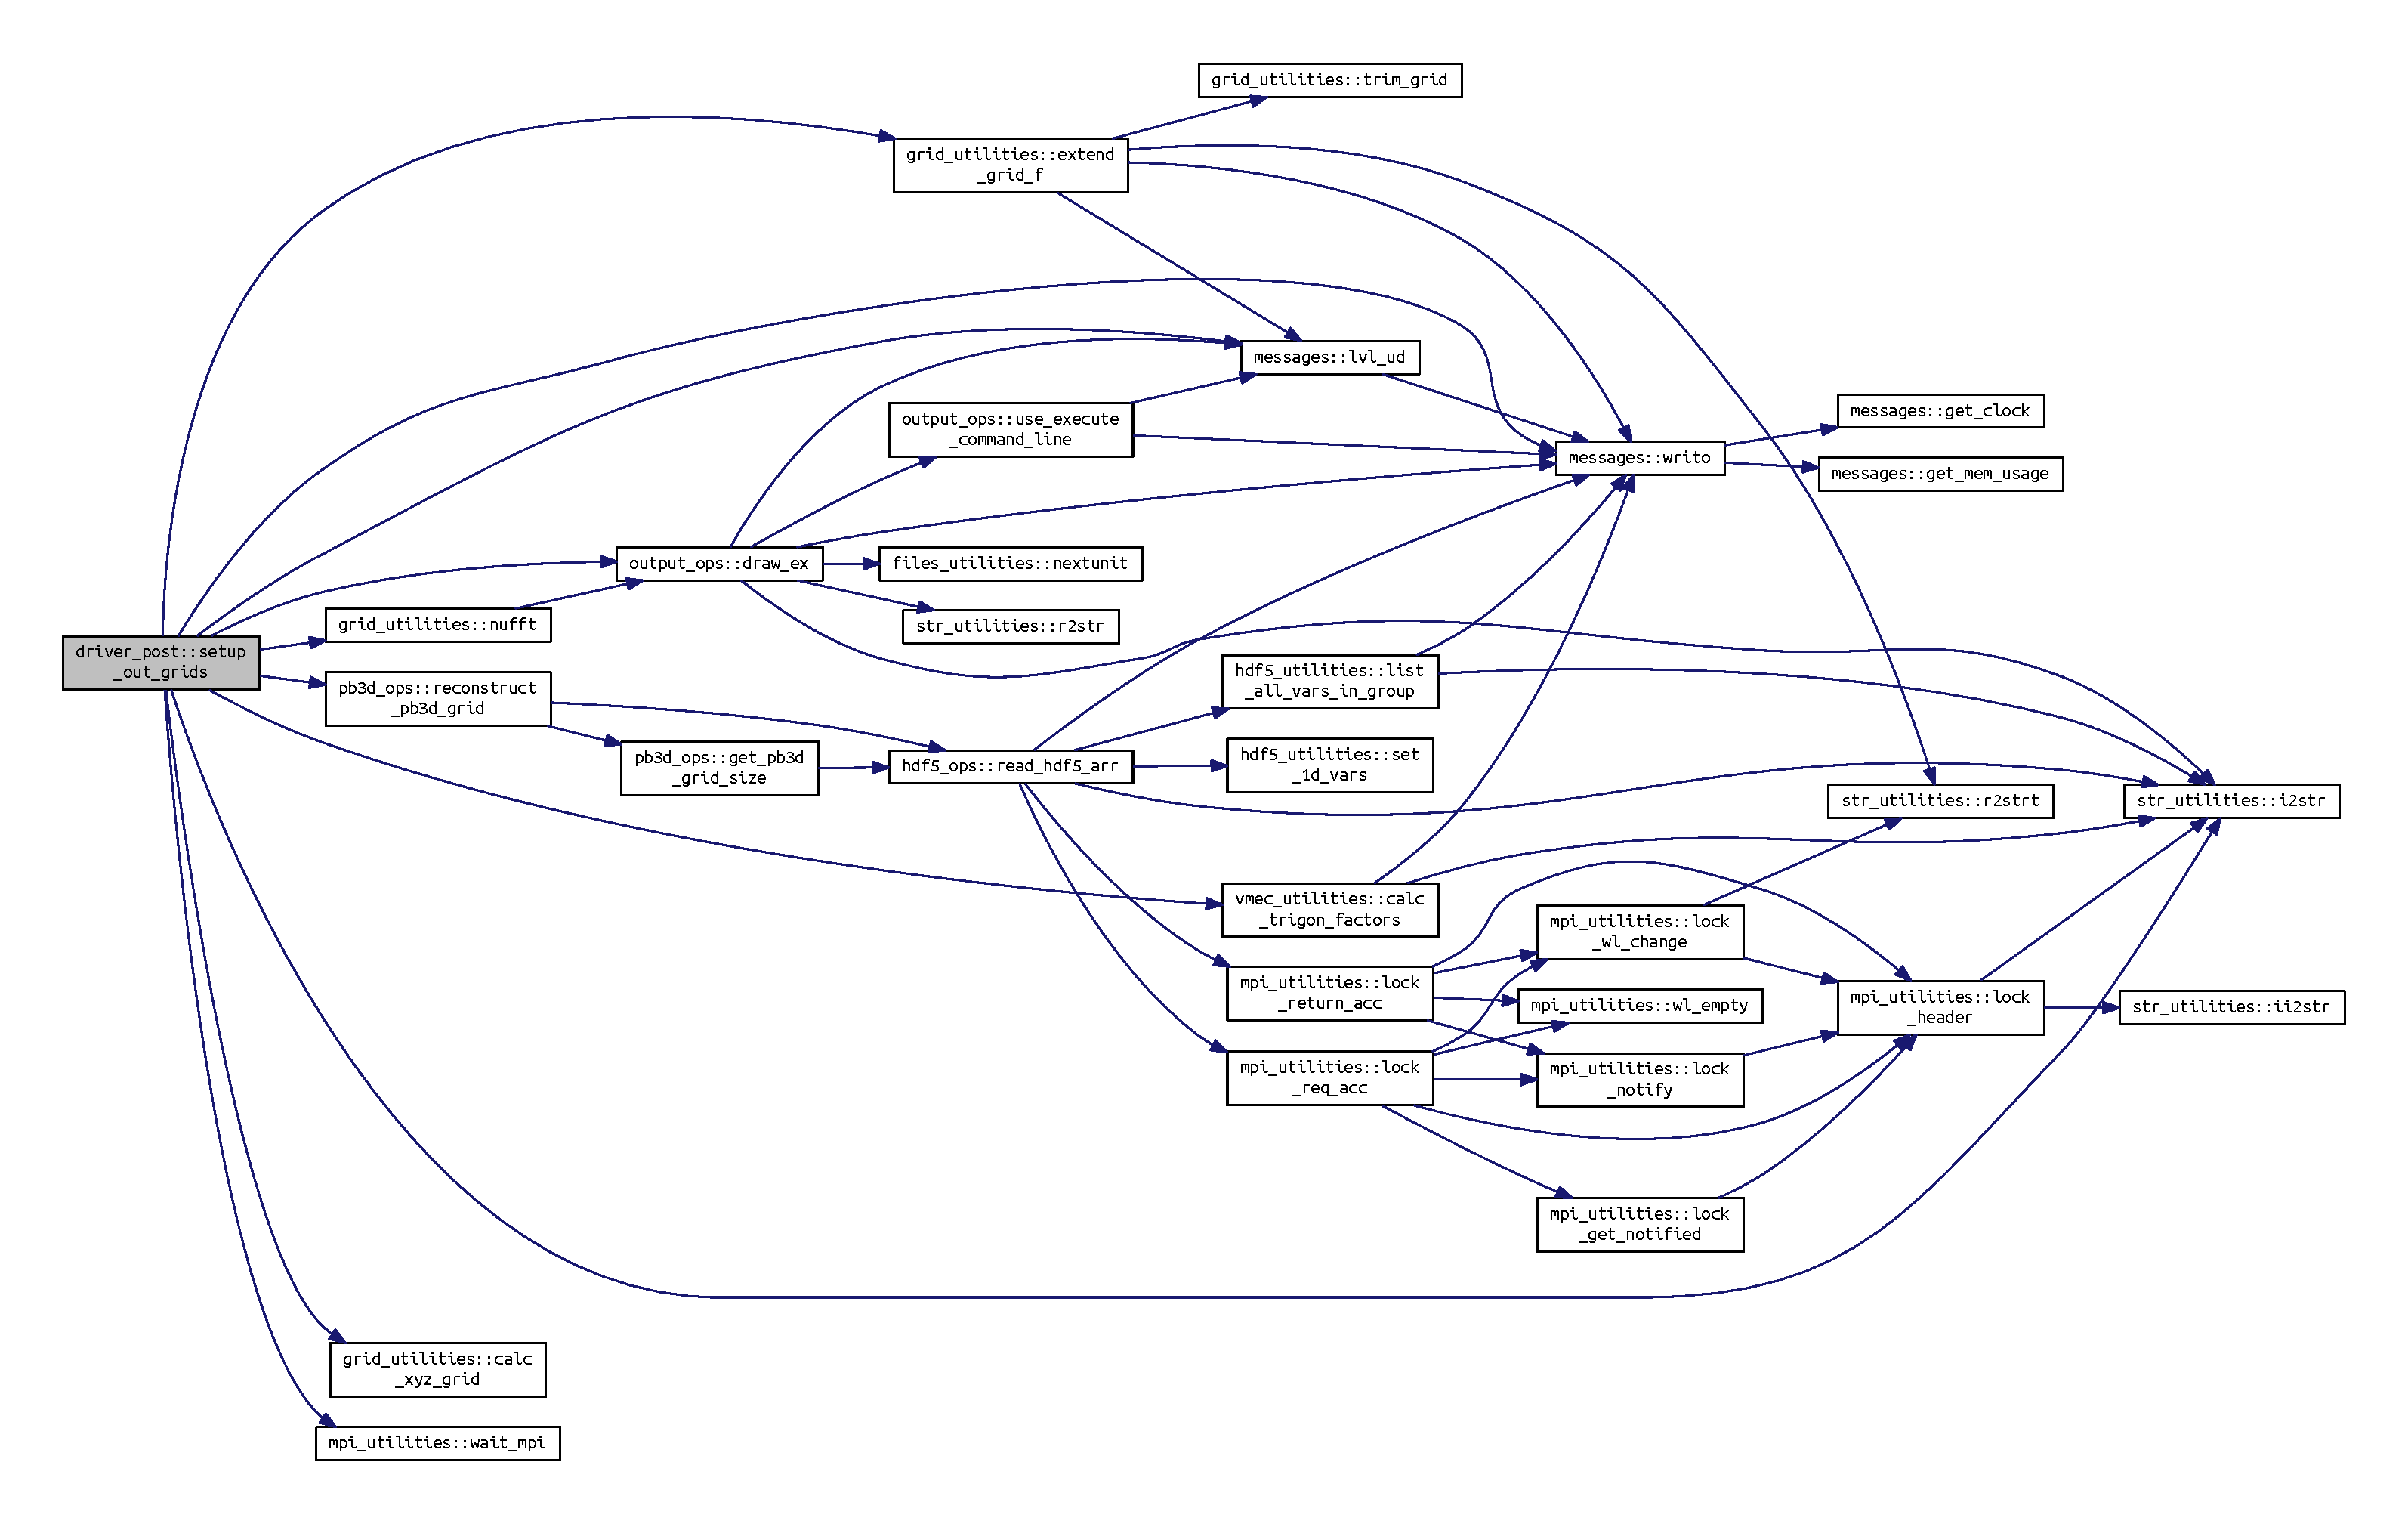
\includegraphics[width=350pt]{namespacedriver__post_a3438685c5fb7302f756c368fb5f940ee_cgraph}
\end{center}
\end{figure}
Here is the caller graph for this function\+:\nopagebreak
\begin{figure}[H]
\begin{center}
\leavevmode
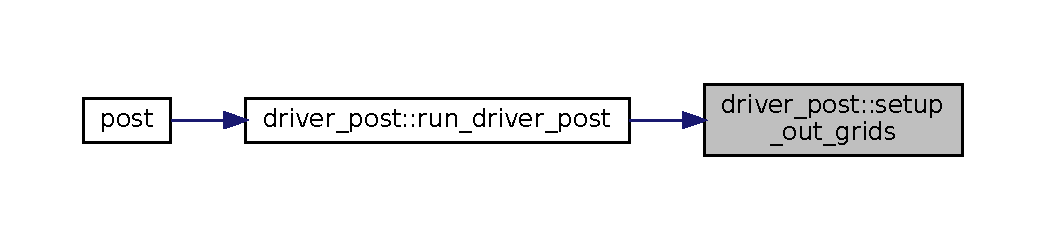
\includegraphics[width=350pt]{namespacedriver__post_a3438685c5fb7302f756c368fb5f940ee_icgraph}
\end{center}
\end{figure}
\mbox{\Hypertarget{namespacedriver__post_a71f9fb1935222111e1c7cfc15c5d0269}\label{namespacedriver__post_a71f9fb1935222111e1c7cfc15c5d0269}} 
\index{driver\_post@{driver\_post}!stop\_post@{stop\_post}}
\index{stop\_post@{stop\_post}!driver\_post@{driver\_post}}
\doxysubsubsection{\texorpdfstring{stop\_post()}{stop\_post()}}
{\footnotesize\ttfamily subroutine, public driver\+\_\+post\+::stop\+\_\+post}



Cleans up main driver for postprocessing. 



Definition at line 816 of file driver\+\_\+\+P\+O\+S\+T.\+f90.

Here is the call graph for this function\+:\nopagebreak
\begin{figure}[H]
\begin{center}
\leavevmode
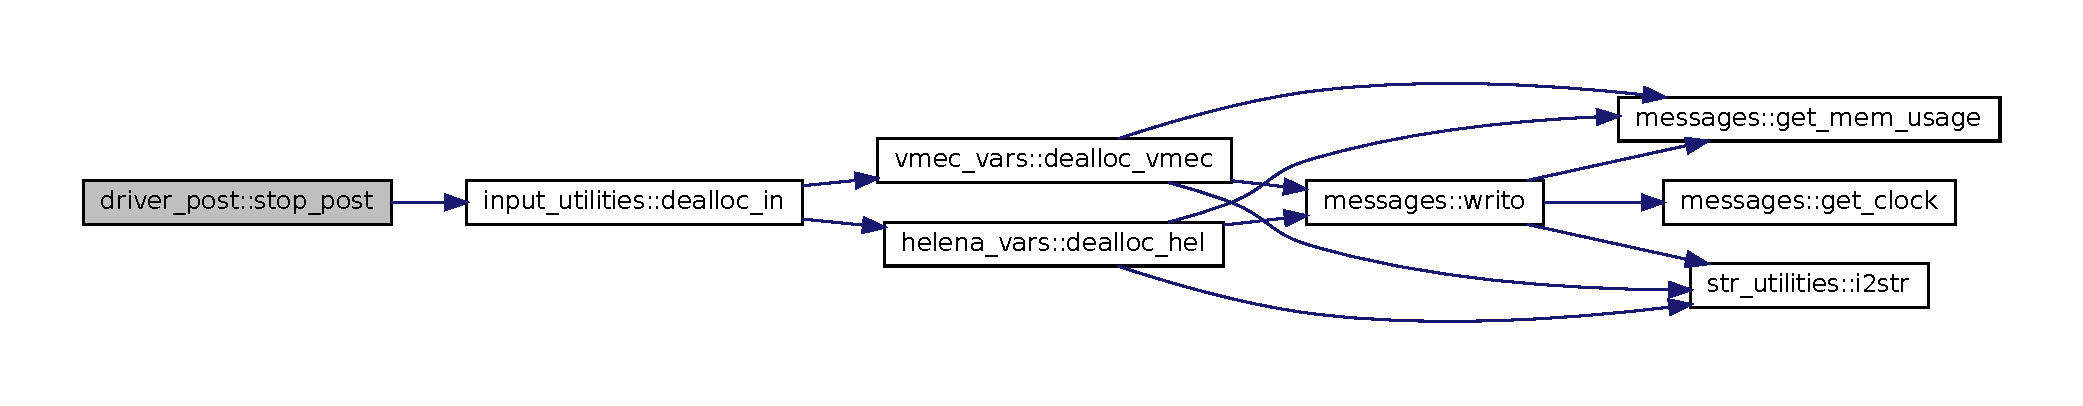
\includegraphics[width=350pt]{namespacedriver__post_a71f9fb1935222111e1c7cfc15c5d0269_cgraph}
\end{center}
\end{figure}
Here is the caller graph for this function\+:\nopagebreak
\begin{figure}[H]
\begin{center}
\leavevmode
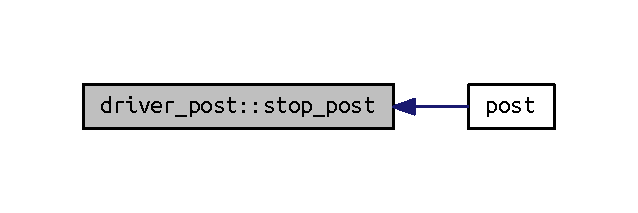
\includegraphics[width=306pt]{namespacedriver__post_a71f9fb1935222111e1c7cfc15c5d0269_icgraph}
\end{center}
\end{figure}
\mbox{\Hypertarget{namespacedriver__post_a4981c6c0e63b862c92ba240f43e22e77}\label{namespacedriver__post_a4981c6c0e63b862c92ba240f43e22e77}} 
\index{driver\_post@{driver\_post}!write\_decomp\_log@{write\_decomp\_log}}
\index{write\_decomp\_log@{write\_decomp\_log}!driver\_post@{driver\_post}}
\doxysubsubsection{\texorpdfstring{write\_decomp\_log()}{write\_decomp\_log()}}
{\footnotesize\ttfamily integer function driver\+\_\+post\+::write\+\_\+decomp\+\_\+log (\begin{DoxyParamCaption}\item[{integer, intent(in)}]{X\+\_\+id,  }\item[{complex(dp), dimension(7), intent(in)}]{E\+\_\+pot\+\_\+int,  }\item[{complex(dp), dimension(2), intent(in)}]{E\+\_\+kin\+\_\+int }\end{DoxyParamCaption})}



Write to decomposition log file. 

\begin{DoxyReturn}{Returns}
ierr 
\end{DoxyReturn}

\begin{DoxyParams}[1]{Parameters}
\mbox{\texttt{ in}}  & {\em x\+\_\+id} & nr. of Eigenvalue \\
\hline
\mbox{\texttt{ in}}  & {\em e\+\_\+pot\+\_\+int} & E\+\_\+pot integrated for requested solutions \\
\hline
\mbox{\texttt{ in}}  & {\em e\+\_\+kin\+\_\+int} & E\+\_\+kin integrated for requested solutions \\
\hline
\end{DoxyParams}


Definition at line 922 of file driver\+\_\+\+P\+O\+S\+T.\+f90.

Here is the call graph for this function\+:\nopagebreak
\begin{figure}[H]
\begin{center}
\leavevmode
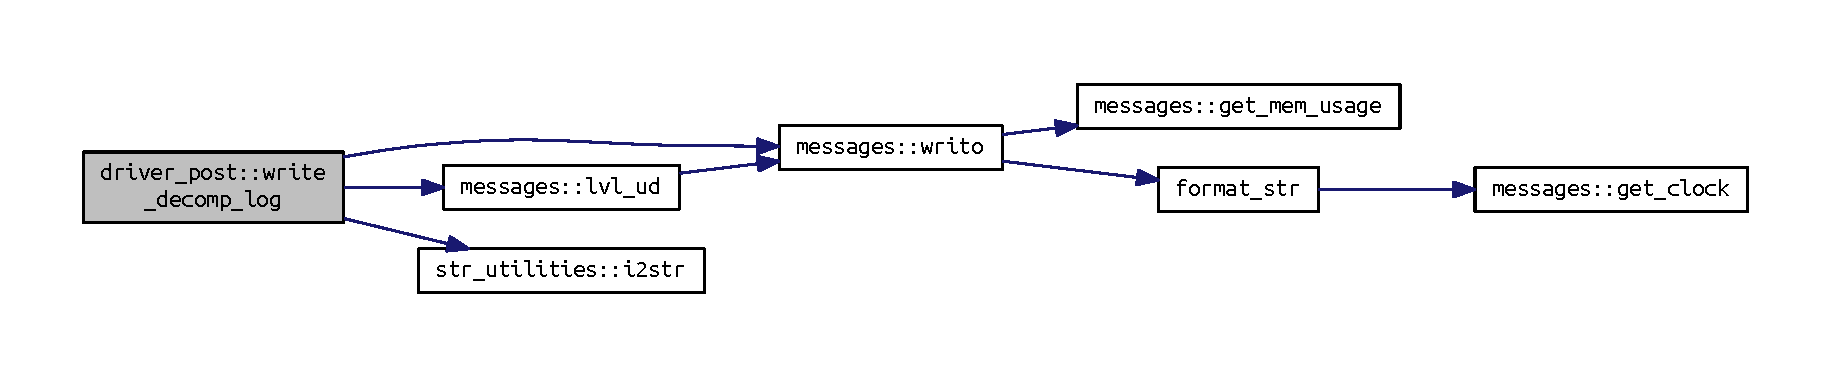
\includegraphics[width=350pt]{namespacedriver__post_a4981c6c0e63b862c92ba240f43e22e77_cgraph}
\end{center}
\end{figure}
Here is the caller graph for this function\+:\nopagebreak
\begin{figure}[H]
\begin{center}
\leavevmode
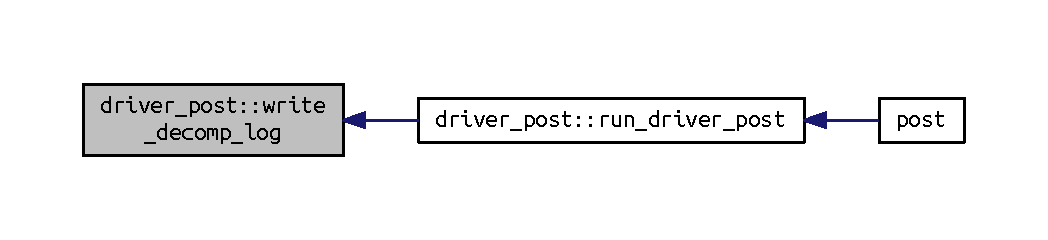
\includegraphics[width=350pt]{namespacedriver__post_a4981c6c0e63b862c92ba240f43e22e77_icgraph}
\end{center}
\end{figure}

\hypertarget{namespacedriver__sol}{}\section{driver\+\_\+sol Module Reference}
\label{namespacedriver__sol}\index{driver\+\_\+sol@{driver\+\_\+sol}}


Driver of the solution part of P\+B3D.  


\subsection*{Functions/\+Subroutines}
\begin{DoxyCompactItemize}
\item 
integer function, public \hyperlink{namespacedriver__sol_ad3b1765b3ecc5f82129bfc683ffc6c5c}{run\+\_\+driver\+\_\+sol} (grid\+\_\+eq, grid\+\_\+X, grid\+\_\+sol, X, vac, sol)
\begin{DoxyCompactList}\small\item\em Main driver of P\+B3D solution part. \end{DoxyCompactList}\item 
integer function \hyperlink{namespacedriver__sol_af1c4ea0286ad714d3f91bb1608e4fc27}{interp\+\_\+v} (mds\+\_\+i, grid\+\_\+i, X\+\_\+i, mds\+\_\+o, grid\+\_\+o, X\+\_\+o)
\begin{DoxyCompactList}\small\item\em Interpolate tensorial perturbation quantities in the third dimension. \end{DoxyCompactList}\end{DoxyCompactItemize}


\subsection{Detailed Description}
Driver of the solution part of P\+B3D. 

\subsection{Function/\+Subroutine Documentation}
\mbox{\Hypertarget{namespacedriver__sol_af1c4ea0286ad714d3f91bb1608e4fc27}\label{namespacedriver__sol_af1c4ea0286ad714d3f91bb1608e4fc27}} 
\index{driver\+\_\+sol@{driver\+\_\+sol}!interp\+\_\+v@{interp\+\_\+v}}
\index{interp\+\_\+v@{interp\+\_\+v}!driver\+\_\+sol@{driver\+\_\+sol}}
\subsubsection{\texorpdfstring{interp\+\_\+v()}{interp\_v()}}
{\footnotesize\ttfamily integer function driver\+\_\+sol\+::interp\+\_\+v (\begin{DoxyParamCaption}\item[{type(modes\+\_\+type), intent(in)}]{mds\+\_\+i,  }\item[{type(\hyperlink{structgrid__vars_1_1grid__type}{grid\+\_\+type}), intent(in)}]{grid\+\_\+i,  }\item[{type(x\+\_\+2\+\_\+type), intent(in), target}]{X\+\_\+i,  }\item[{type(modes\+\_\+type), intent(in)}]{mds\+\_\+o,  }\item[{type(\hyperlink{structgrid__vars_1_1grid__type}{grid\+\_\+type}), intent(in)}]{grid\+\_\+o,  }\item[{type(x\+\_\+2\+\_\+type), intent(inout), target}]{X\+\_\+o }\end{DoxyParamCaption})}



Interpolate tensorial perturbation quantities in the third dimension. 

The input grid should not be divided, whereas the output grid can be.

The procedure considers all possible mode number combinations. For {\ttfamily X\+\_\+style} 2 (fast), each secondary mode only lives in a certain normal range of the plasma. Therefore, each secondary mode pair also has a limited normal range, given by the overlap of the ranges of the members.

The interpolated mode number combinations have a normal range that might slightly differ from the input ranges, in which case extrapolation can be done if the method allows for it.

\begin{DoxyNote}{Note}
If the input grid is too coarse, but the interpolated grid is not, it is in theory possible that there are mode numbers and therefore mode number pairs that exist in the input grid, though they do so in the interpolated grid. In this case, they can not be calculated and are currently set to zero. However, the current implementation of \hyperlink{namespacex__ops_a504451aabcab7d6f0fa59feae08ef8dd}{setup\+\_\+modes()} produces an error if less than the full range of mode numbers is accurately present.
\end{DoxyNote}

\begin{DoxyParams}[1]{Parameters}
\mbox{\tt in}  & {\em mds\+\_\+i} & general modes variables for input\\
\hline
\mbox{\tt in}  & {\em grid\+\_\+i} & grid at which {\ttfamily X\+\_\+i} is tabulated\\
\hline
\mbox{\tt in}  & {\em x\+\_\+i} & tensorial perturbation variable on input grid\\
\hline
\mbox{\tt in}  & {\em mds\+\_\+o} & general modes variables for output\\
\hline
\mbox{\tt in}  & {\em grid\+\_\+o} & grid at which {\ttfamily X\+\_\+o} is interpolated\\
\hline
\mbox{\tt in,out}  & {\em x\+\_\+o} & interpolated tensorial perturbation variable \\
\hline
\end{DoxyParams}


Definition at line 278 of file driver\+\_\+sol.\+f90.

Here is the call graph for this function\+:\nopagebreak
\begin{figure}[H]
\begin{center}
\leavevmode
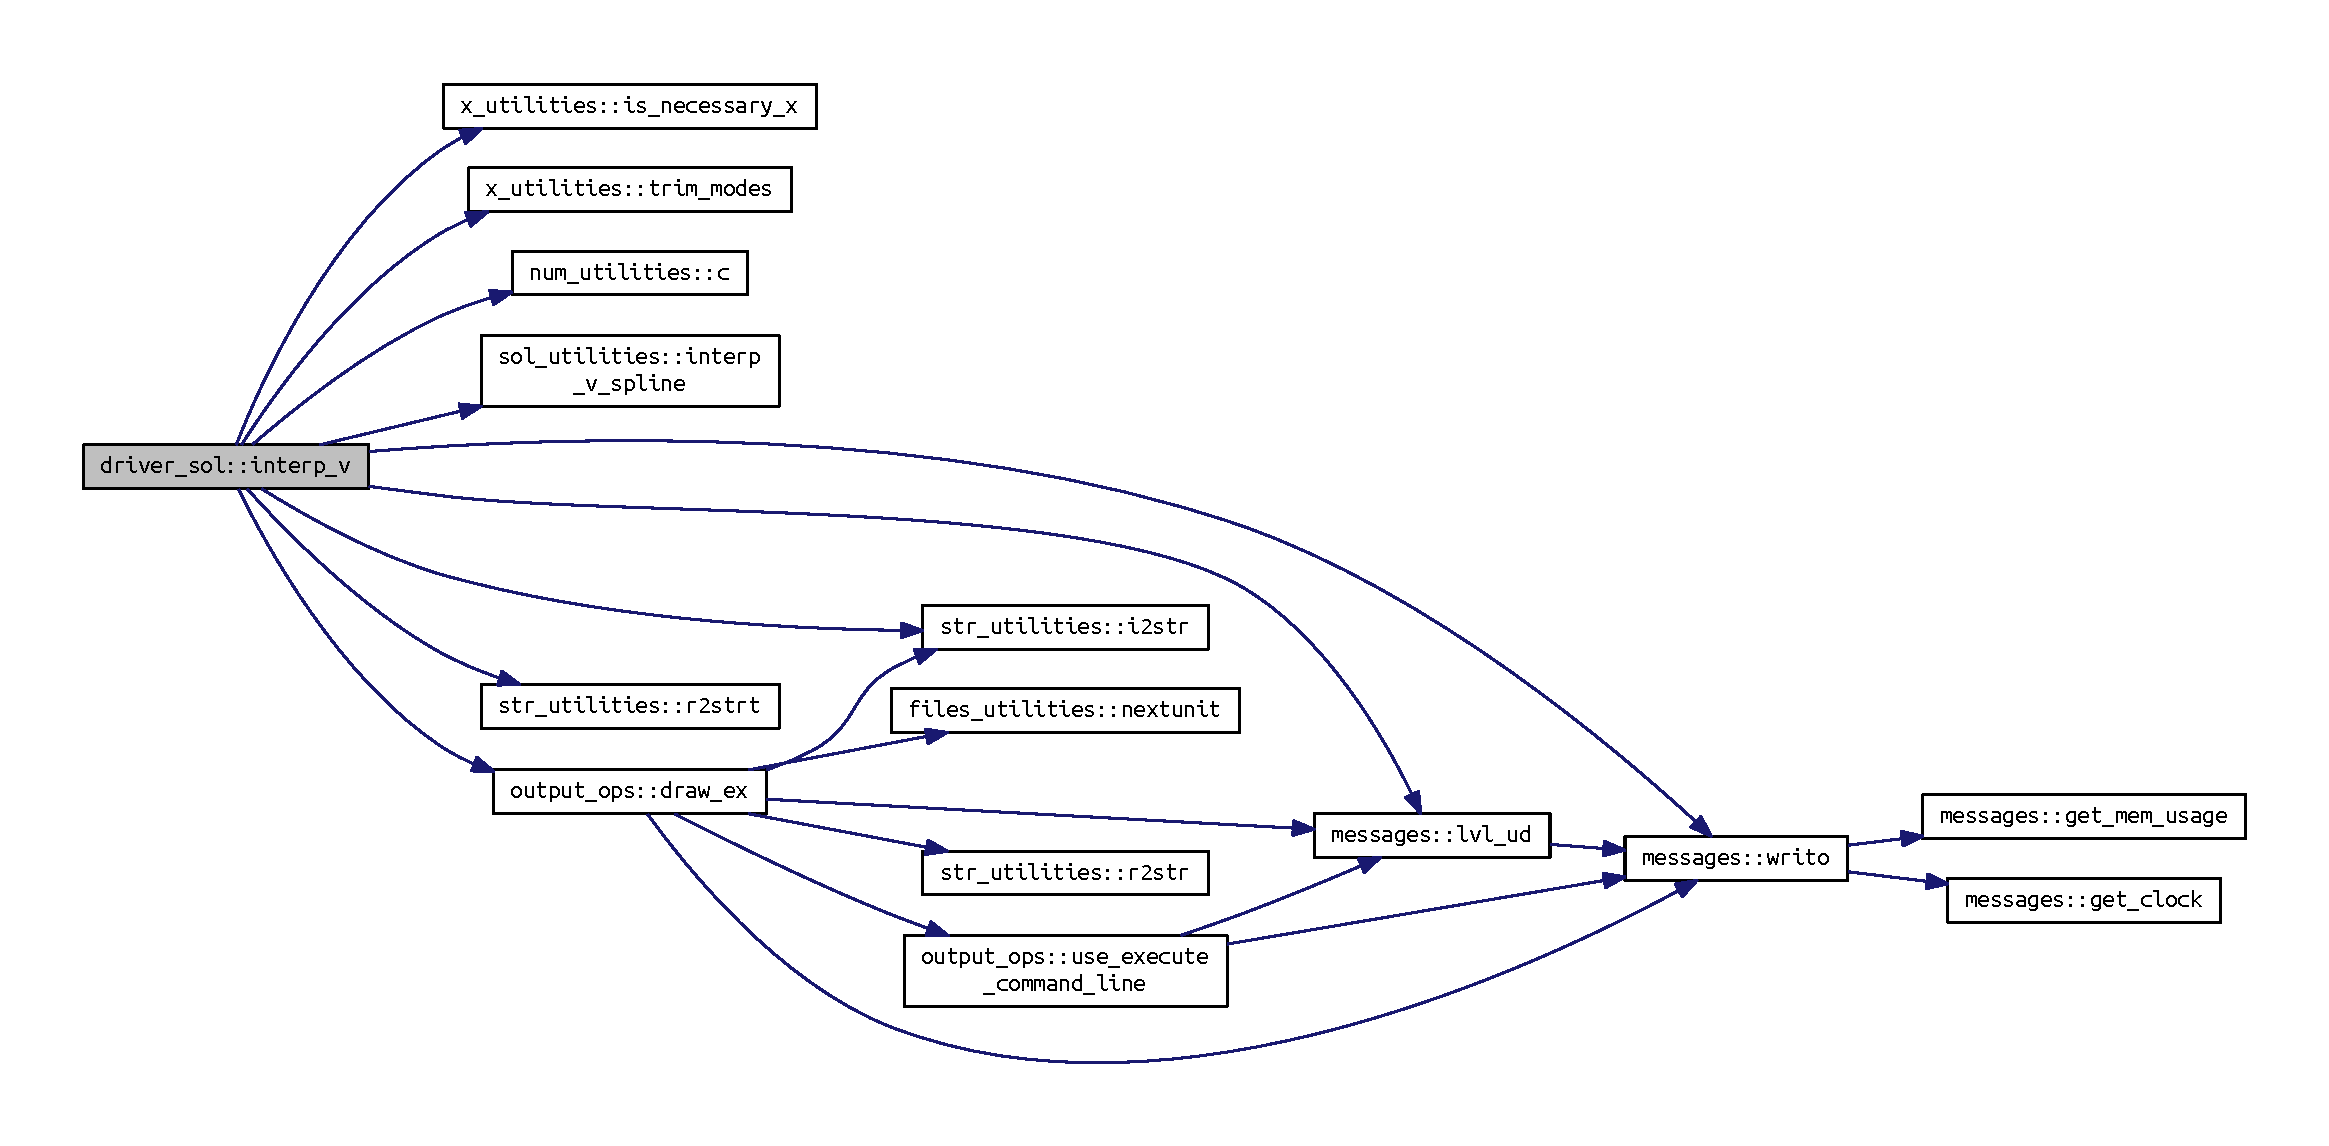
\includegraphics[width=350pt]{namespacedriver__sol_af1c4ea0286ad714d3f91bb1608e4fc27_cgraph}
\end{center}
\end{figure}
Here is the caller graph for this function\+:\nopagebreak
\begin{figure}[H]
\begin{center}
\leavevmode
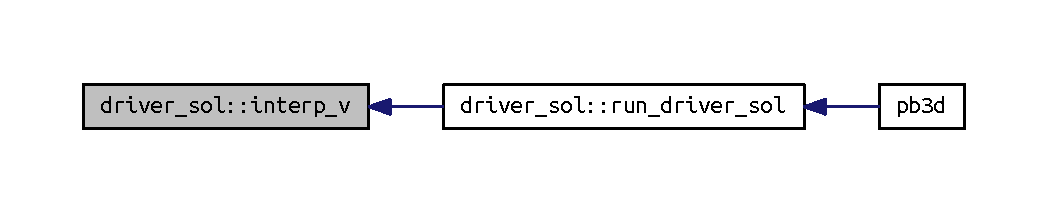
\includegraphics[width=350pt]{namespacedriver__sol_af1c4ea0286ad714d3f91bb1608e4fc27_icgraph}
\end{center}
\end{figure}
\mbox{\Hypertarget{namespacedriver__sol_ad3b1765b3ecc5f82129bfc683ffc6c5c}\label{namespacedriver__sol_ad3b1765b3ecc5f82129bfc683ffc6c5c}} 
\index{driver\+\_\+sol@{driver\+\_\+sol}!run\+\_\+driver\+\_\+sol@{run\+\_\+driver\+\_\+sol}}
\index{run\+\_\+driver\+\_\+sol@{run\+\_\+driver\+\_\+sol}!driver\+\_\+sol@{driver\+\_\+sol}}
\subsubsection{\texorpdfstring{run\+\_\+driver\+\_\+sol()}{run\_driver\_sol()}}
{\footnotesize\ttfamily integer function, public driver\+\_\+sol\+::run\+\_\+driver\+\_\+sol (\begin{DoxyParamCaption}\item[{type(\hyperlink{structgrid__vars_1_1grid__type}{grid\+\_\+type}), intent(in)}]{grid\+\_\+eq,  }\item[{type(\hyperlink{structgrid__vars_1_1grid__type}{grid\+\_\+type}), intent(in), target}]{grid\+\_\+X,  }\item[{type(\hyperlink{structgrid__vars_1_1grid__type}{grid\+\_\+type}), intent(inout)}]{grid\+\_\+sol,  }\item[{type(x\+\_\+2\+\_\+type), intent(in)}]{X,  }\item[{type(\hyperlink{structvac__vars_1_1vac__type}{vac\+\_\+type}), intent(inout)}]{vac,  }\item[{type(\hyperlink{structsol__vars_1_1sol__type}{sol\+\_\+type}), intent(inout)}]{sol }\end{DoxyParamCaption})}



Main driver of P\+B3D solution part. 


\begin{DoxyItemize}
\item sets up\+:
\begin{DoxyItemize}
\item {\ttfamily grid\+\_\+sol} (only first Richardson level)
\item {\ttfamily sol} 
\end{DoxyItemize}
\item writes to H\+D\+F5\+:
\begin{DoxyItemize}
\item {\ttfamily grid\+\_\+sol} (only first Richardson level)
\item {\ttfamily sol} 
\end{DoxyItemize}
\item deallocates\+:
\begin{DoxyItemize}
\item sol before setting up (but after guess)
\end{DoxyItemize}
\end{DoxyItemize}

\begin{DoxyReturn}{Returns}
ierr
\end{DoxyReturn}

\begin{DoxyParams}[1]{Parameters}
\mbox{\tt in}  & {\em grid\+\_\+eq} & equilibrium grid\\
\hline
\mbox{\tt in}  & {\em grid\+\_\+x} & perturbation grid\\
\hline
\mbox{\tt in,out}  & {\em grid\+\_\+sol} & solution grid\\
\hline
\mbox{\tt in}  & {\em x} & integrated tensorial perturbation variables\\
\hline
\mbox{\tt in,out}  & {\em vac} & vacuum variables\\
\hline
\mbox{\tt in,out}  & {\em sol} & solution variables \\
\hline
\end{DoxyParams}


Definition at line 43 of file driver\+\_\+sol.\+f90.

Here is the call graph for this function\+:\nopagebreak
\begin{figure}[H]
\begin{center}
\leavevmode
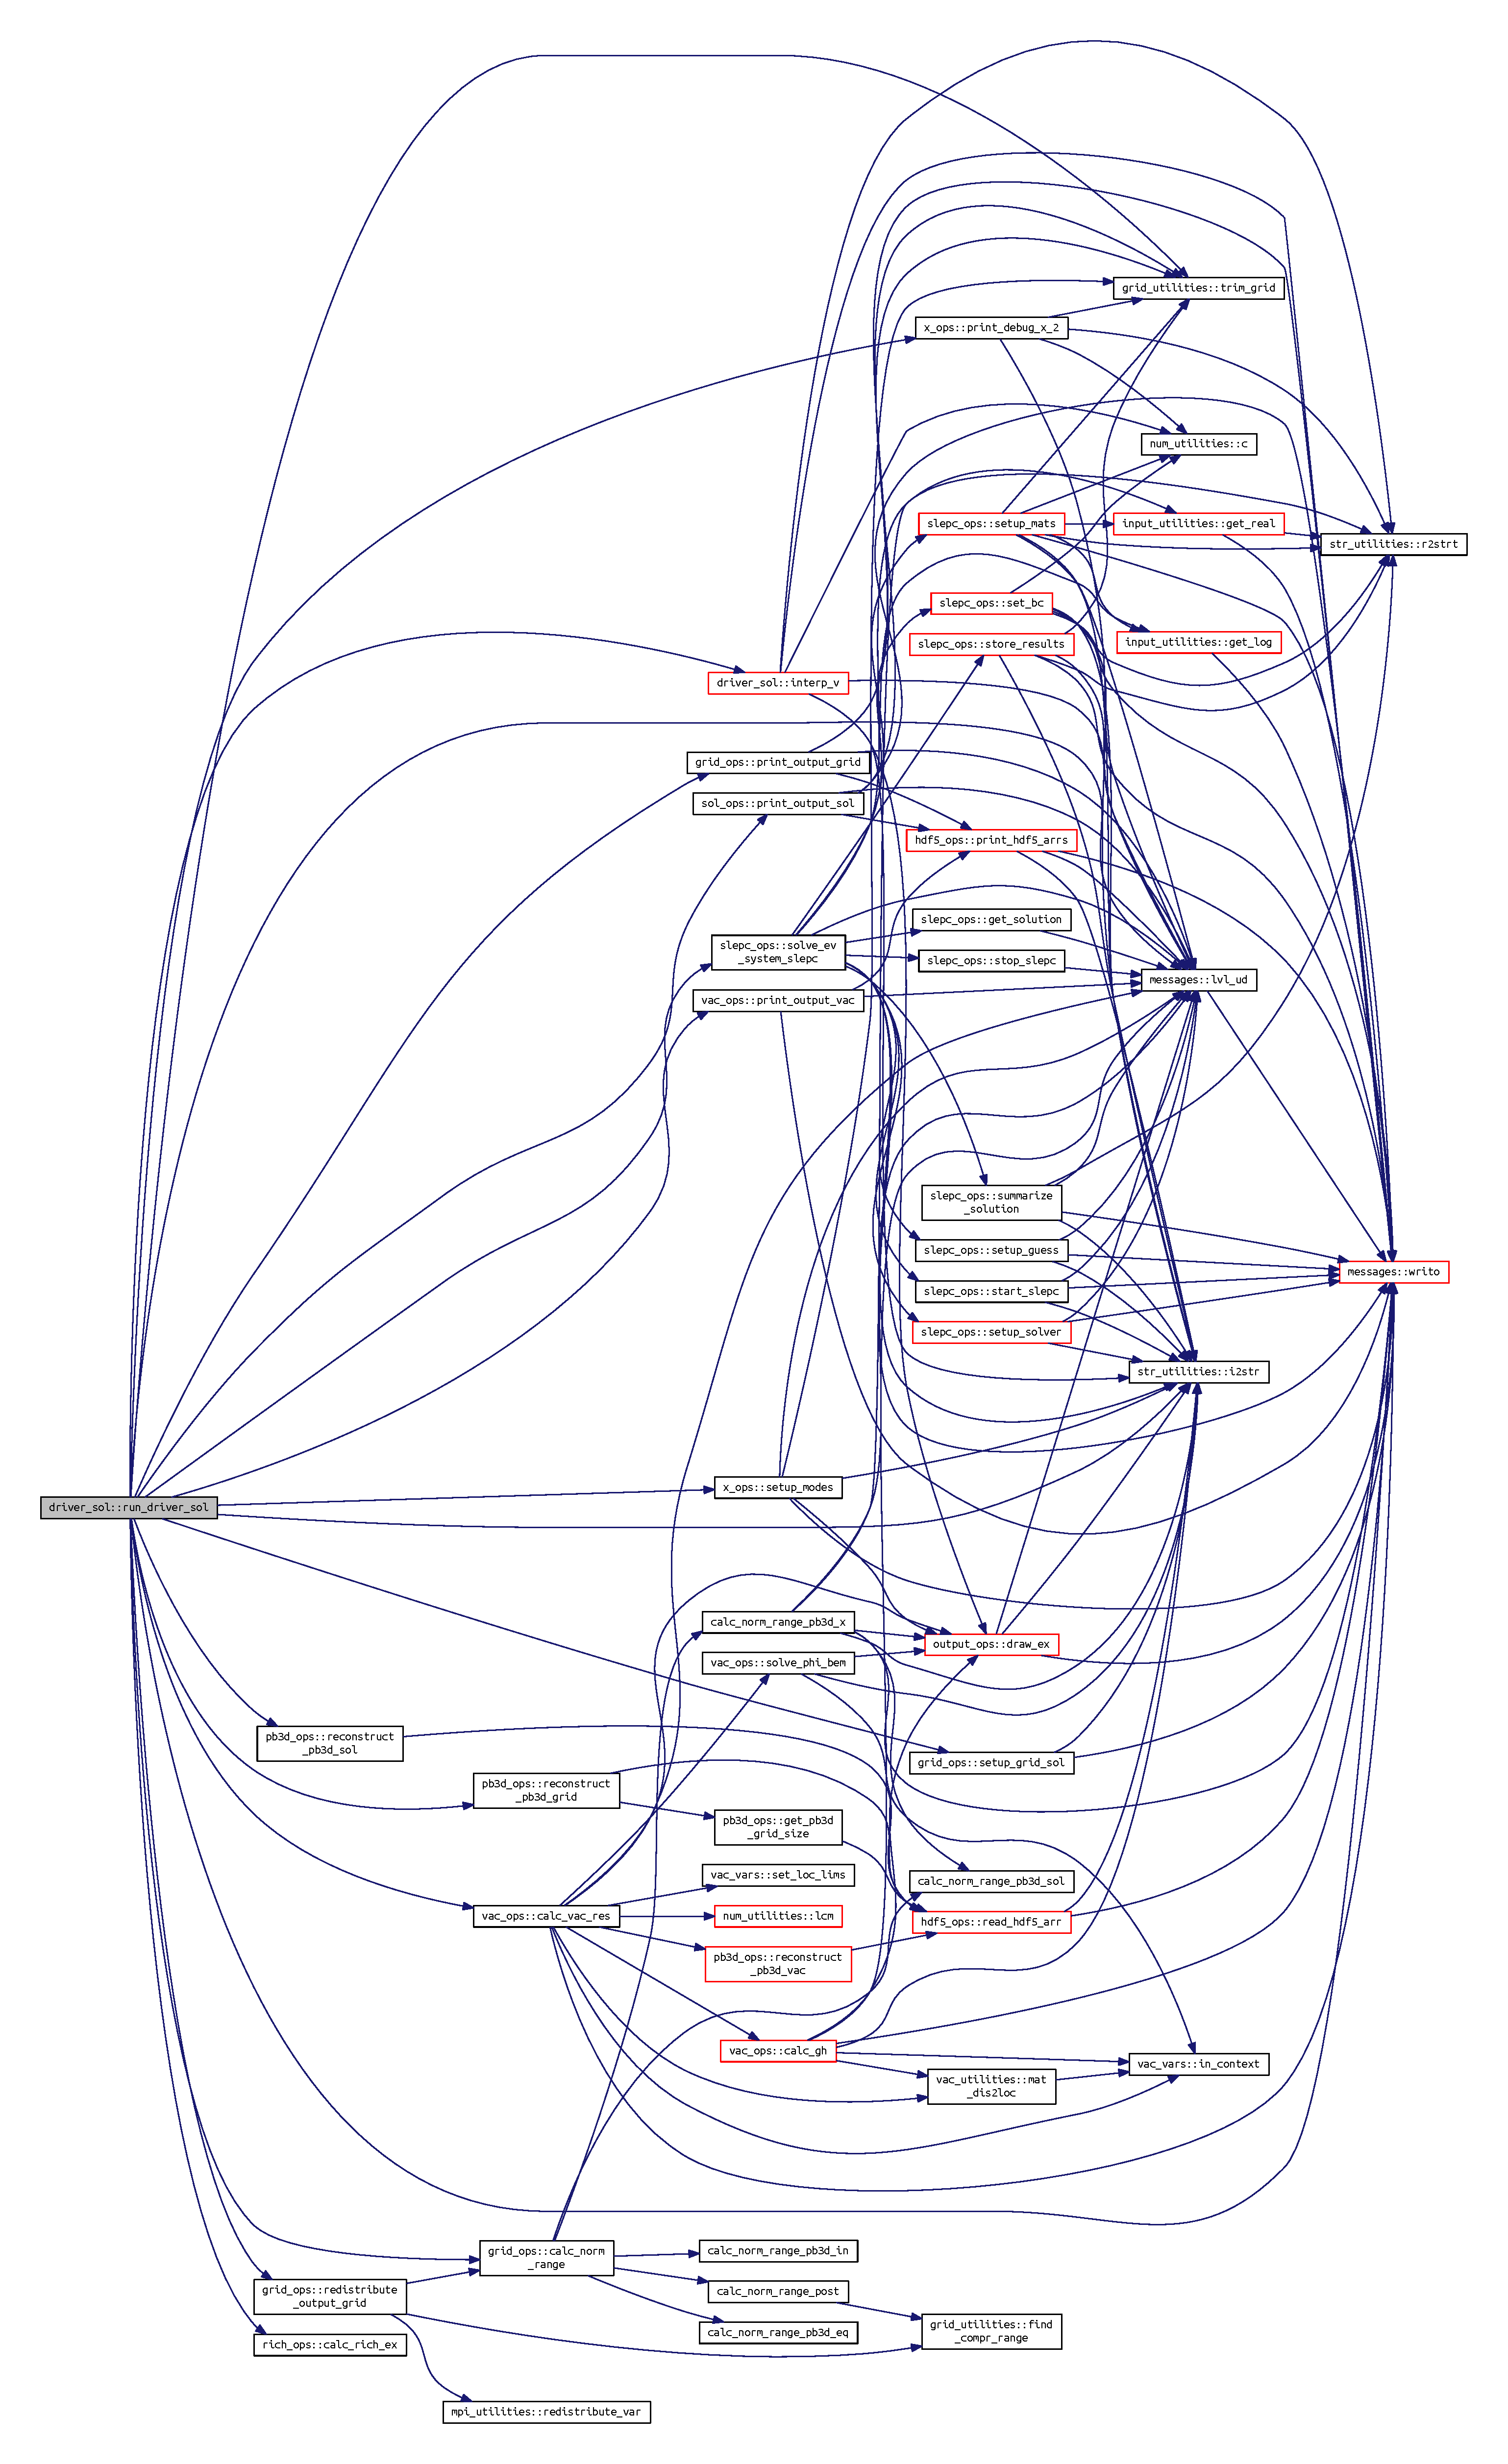
\includegraphics[width=350pt]{namespacedriver__sol_ad3b1765b3ecc5f82129bfc683ffc6c5c_cgraph}
\end{center}
\end{figure}
Here is the caller graph for this function\+:\nopagebreak
\begin{figure}[H]
\begin{center}
\leavevmode
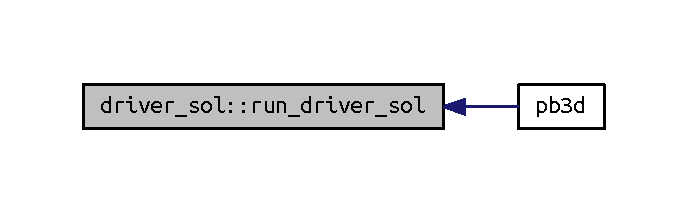
\includegraphics[width=330pt]{namespacedriver__sol_ad3b1765b3ecc5f82129bfc683ffc6c5c_icgraph}
\end{center}
\end{figure}

\hypertarget{namespacedriver__x}{}\section{driver\+\_\+x Module Reference}
\label{namespacedriver__x}\index{driver\+\_\+x@{driver\+\_\+x}}
\subsection*{Functions/\+Subroutines}
\begin{DoxyCompactItemize}
\item 
integer function, public \hyperlink{namespacedriver__x_ada3d72a0929daaa5e3da585246d62281}{run\+\_\+driver\+\_\+x} (grid\+\_\+eq, grid\+\_\+eq\+\_\+B, grid\+\_\+X, grid\+\_\+\+X\+\_\+B, eq\+\_\+1, eq\+\_\+2, X\+\_\+1, X\+\_\+2)
\item 
integer function \hyperlink{namespacedriver__x_a2b82a9bc6c0f4af9f3468d03fedc008e}{run\+\_\+driver\+\_\+x\+\_\+0} (grid\+\_\+eq, grid\+\_\+eq\+\_\+B, grid\+\_\+X, grid\+\_\+\+X\+\_\+B, eq\+\_\+1, eq\+\_\+2, eq\+\_\+2\+\_\+B)
\item 
integer function \hyperlink{namespacedriver__x_a454779cefa6da3714d32eedcec0ef7de}{run\+\_\+driver\+\_\+x\+\_\+1} (grid\+\_\+eq, grid\+\_\+X, eq\+\_\+1, eq\+\_\+2, X\+\_\+1)
\item 
integer function \hyperlink{namespacedriver__x_ad3924b3d66f336f0a9a9559eafffec8e}{run\+\_\+driver\+\_\+x\+\_\+2} (grid\+\_\+eq\+\_\+B, grid\+\_\+X, grid\+\_\+\+X\+\_\+B, eq\+\_\+1, eq\+\_\+2\+\_\+B, X\+\_\+1, X\+\_\+2\+\_\+int)
\item 
subroutine \hyperlink{namespacedriver__x_aca49d362e21df044e21d5ba4b2599cf4}{print\+\_\+info\+\_\+x\+\_\+2} ()
\end{DoxyCompactItemize}


\subsection{Function/\+Subroutine Documentation}
\mbox{\Hypertarget{namespacedriver__x_aca49d362e21df044e21d5ba4b2599cf4}\label{namespacedriver__x_aca49d362e21df044e21d5ba4b2599cf4}} 
\index{driver\+\_\+x@{driver\+\_\+x}!print\+\_\+info\+\_\+x\+\_\+2@{print\+\_\+info\+\_\+x\+\_\+2}}
\index{print\+\_\+info\+\_\+x\+\_\+2@{print\+\_\+info\+\_\+x\+\_\+2}!driver\+\_\+x@{driver\+\_\+x}}
\subsubsection{\texorpdfstring{print\+\_\+info\+\_\+x\+\_\+2()}{print\_info\_x\_2()}}
{\footnotesize\ttfamily subroutine driver\+\_\+x\+::print\+\_\+info\+\_\+x\+\_\+2 (\begin{DoxyParamCaption}{ }\end{DoxyParamCaption})}



Definition at line 820 of file driver\+\_\+\+X.\+f90.

Here is the call graph for this function\+:
\nopagebreak
\begin{figure}[H]
\begin{center}
\leavevmode
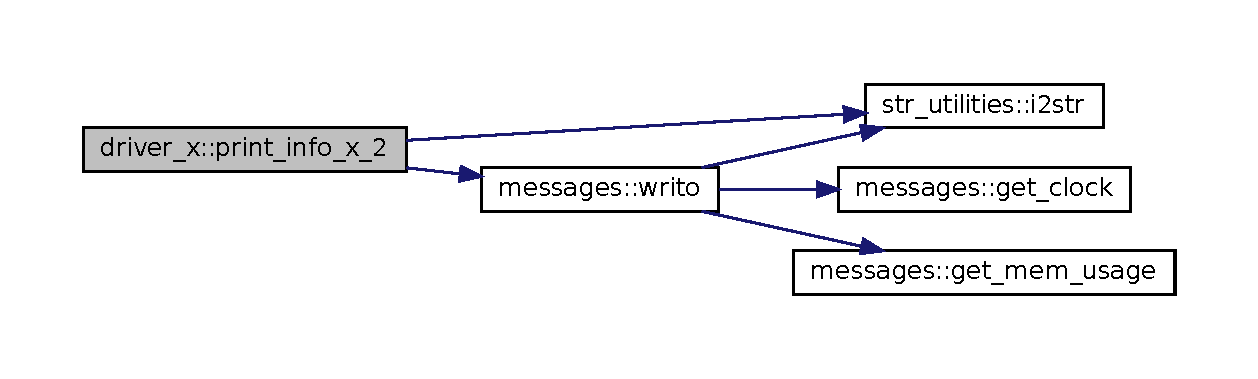
\includegraphics[width=350pt]{namespacedriver__x_aca49d362e21df044e21d5ba4b2599cf4_cgraph}
\end{center}
\end{figure}
Here is the caller graph for this function\+:
\nopagebreak
\begin{figure}[H]
\begin{center}
\leavevmode
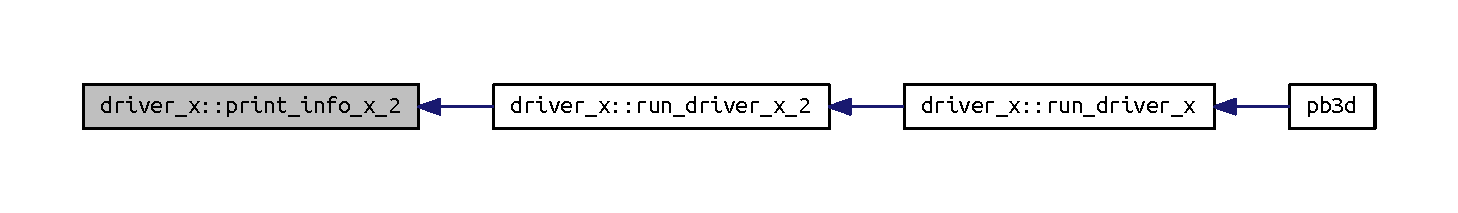
\includegraphics[width=350pt]{namespacedriver__x_aca49d362e21df044e21d5ba4b2599cf4_icgraph}
\end{center}
\end{figure}
\mbox{\Hypertarget{namespacedriver__x_ada3d72a0929daaa5e3da585246d62281}\label{namespacedriver__x_ada3d72a0929daaa5e3da585246d62281}} 
\index{driver\+\_\+x@{driver\+\_\+x}!run\+\_\+driver\+\_\+x@{run\+\_\+driver\+\_\+x}}
\index{run\+\_\+driver\+\_\+x@{run\+\_\+driver\+\_\+x}!driver\+\_\+x@{driver\+\_\+x}}
\subsubsection{\texorpdfstring{run\+\_\+driver\+\_\+x()}{run\_driver\_x()}}
{\footnotesize\ttfamily integer function, public driver\+\_\+x\+::run\+\_\+driver\+\_\+x (\begin{DoxyParamCaption}\item[{type(grid\+\_\+type), intent(inout), target}]{grid\+\_\+eq,  }\item[{type(grid\+\_\+type), intent(inout), pointer}]{grid\+\_\+eq\+\_\+B,  }\item[{type(grid\+\_\+type), intent(inout), target}]{grid\+\_\+X,  }\item[{type(grid\+\_\+type), intent(inout), pointer}]{grid\+\_\+\+X\+\_\+B,  }\item[{type(eq\+\_\+1\+\_\+type), intent(in)}]{eq\+\_\+1,  }\item[{type(eq\+\_\+2\+\_\+type), intent(inout), target}]{eq\+\_\+2,  }\item[{type(x\+\_\+1\+\_\+type), intent(inout)}]{X\+\_\+1,  }\item[{type(x\+\_\+2\+\_\+type), intent(inout)}]{X\+\_\+2 }\end{DoxyParamCaption})}



Definition at line 49 of file driver\+\_\+\+X.\+f90.

Here is the call graph for this function\+:
\nopagebreak
\begin{figure}[H]
\begin{center}
\leavevmode
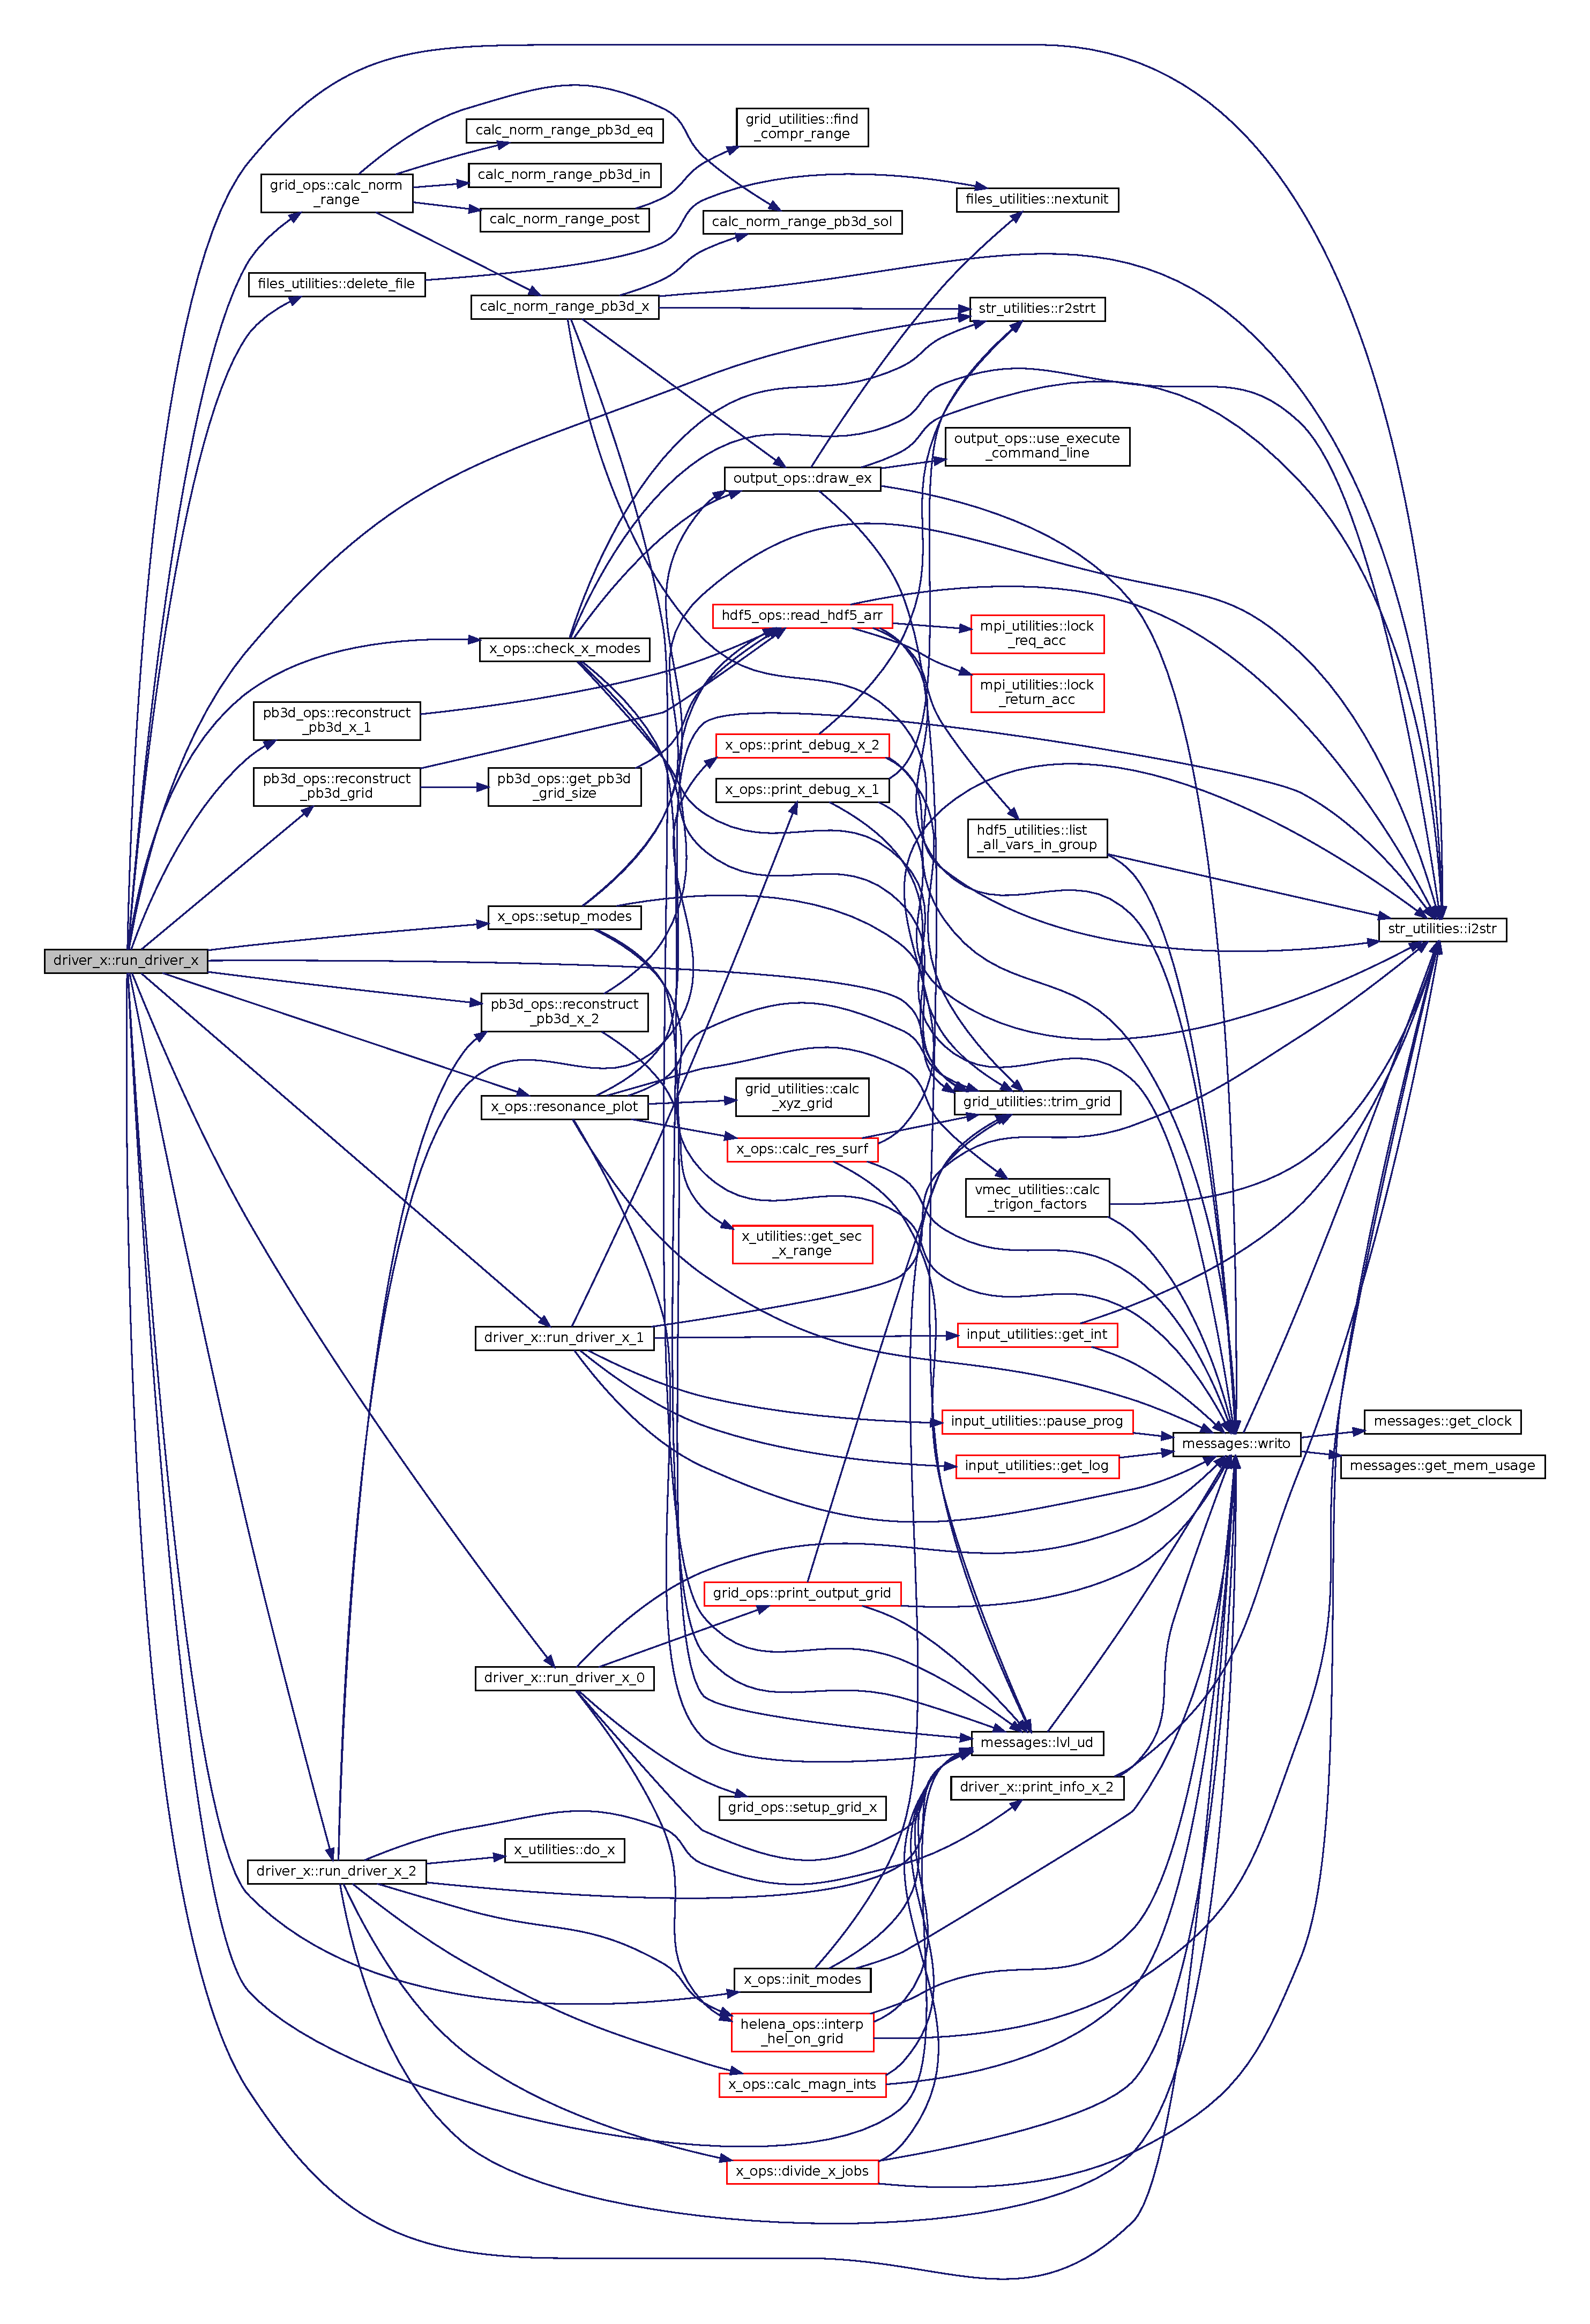
\includegraphics[width=350pt]{namespacedriver__x_ada3d72a0929daaa5e3da585246d62281_cgraph}
\end{center}
\end{figure}
Here is the caller graph for this function\+:
\nopagebreak
\begin{figure}[H]
\begin{center}
\leavevmode
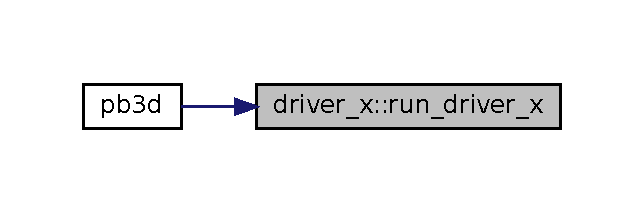
\includegraphics[width=306pt]{namespacedriver__x_ada3d72a0929daaa5e3da585246d62281_icgraph}
\end{center}
\end{figure}
\mbox{\Hypertarget{namespacedriver__x_a2b82a9bc6c0f4af9f3468d03fedc008e}\label{namespacedriver__x_a2b82a9bc6c0f4af9f3468d03fedc008e}} 
\index{driver\+\_\+x@{driver\+\_\+x}!run\+\_\+driver\+\_\+x\+\_\+0@{run\+\_\+driver\+\_\+x\+\_\+0}}
\index{run\+\_\+driver\+\_\+x\+\_\+0@{run\+\_\+driver\+\_\+x\+\_\+0}!driver\+\_\+x@{driver\+\_\+x}}
\subsubsection{\texorpdfstring{run\+\_\+driver\+\_\+x\+\_\+0()}{run\_driver\_x\_0()}}
{\footnotesize\ttfamily integer function driver\+\_\+x\+::run\+\_\+driver\+\_\+x\+\_\+0 (\begin{DoxyParamCaption}\item[{type(grid\+\_\+type), intent(in), target}]{grid\+\_\+eq,  }\item[{type(grid\+\_\+type), intent(in), pointer}]{grid\+\_\+eq\+\_\+B,  }\item[{type(grid\+\_\+type), intent(inout), target}]{grid\+\_\+X,  }\item[{type(grid\+\_\+type), intent(inout), pointer}]{grid\+\_\+\+X\+\_\+B,  }\item[{type(eq\+\_\+1\+\_\+type), intent(in)}]{eq\+\_\+1,  }\item[{type(eq\+\_\+2\+\_\+type), intent(inout), target}]{eq\+\_\+2,  }\item[{type(eq\+\_\+2\+\_\+type), intent(inout), pointer}]{eq\+\_\+2\+\_\+B }\end{DoxyParamCaption})}



Definition at line 229 of file driver\+\_\+\+X.\+f90.

Here is the call graph for this function\+:
\nopagebreak
\begin{figure}[H]
\begin{center}
\leavevmode
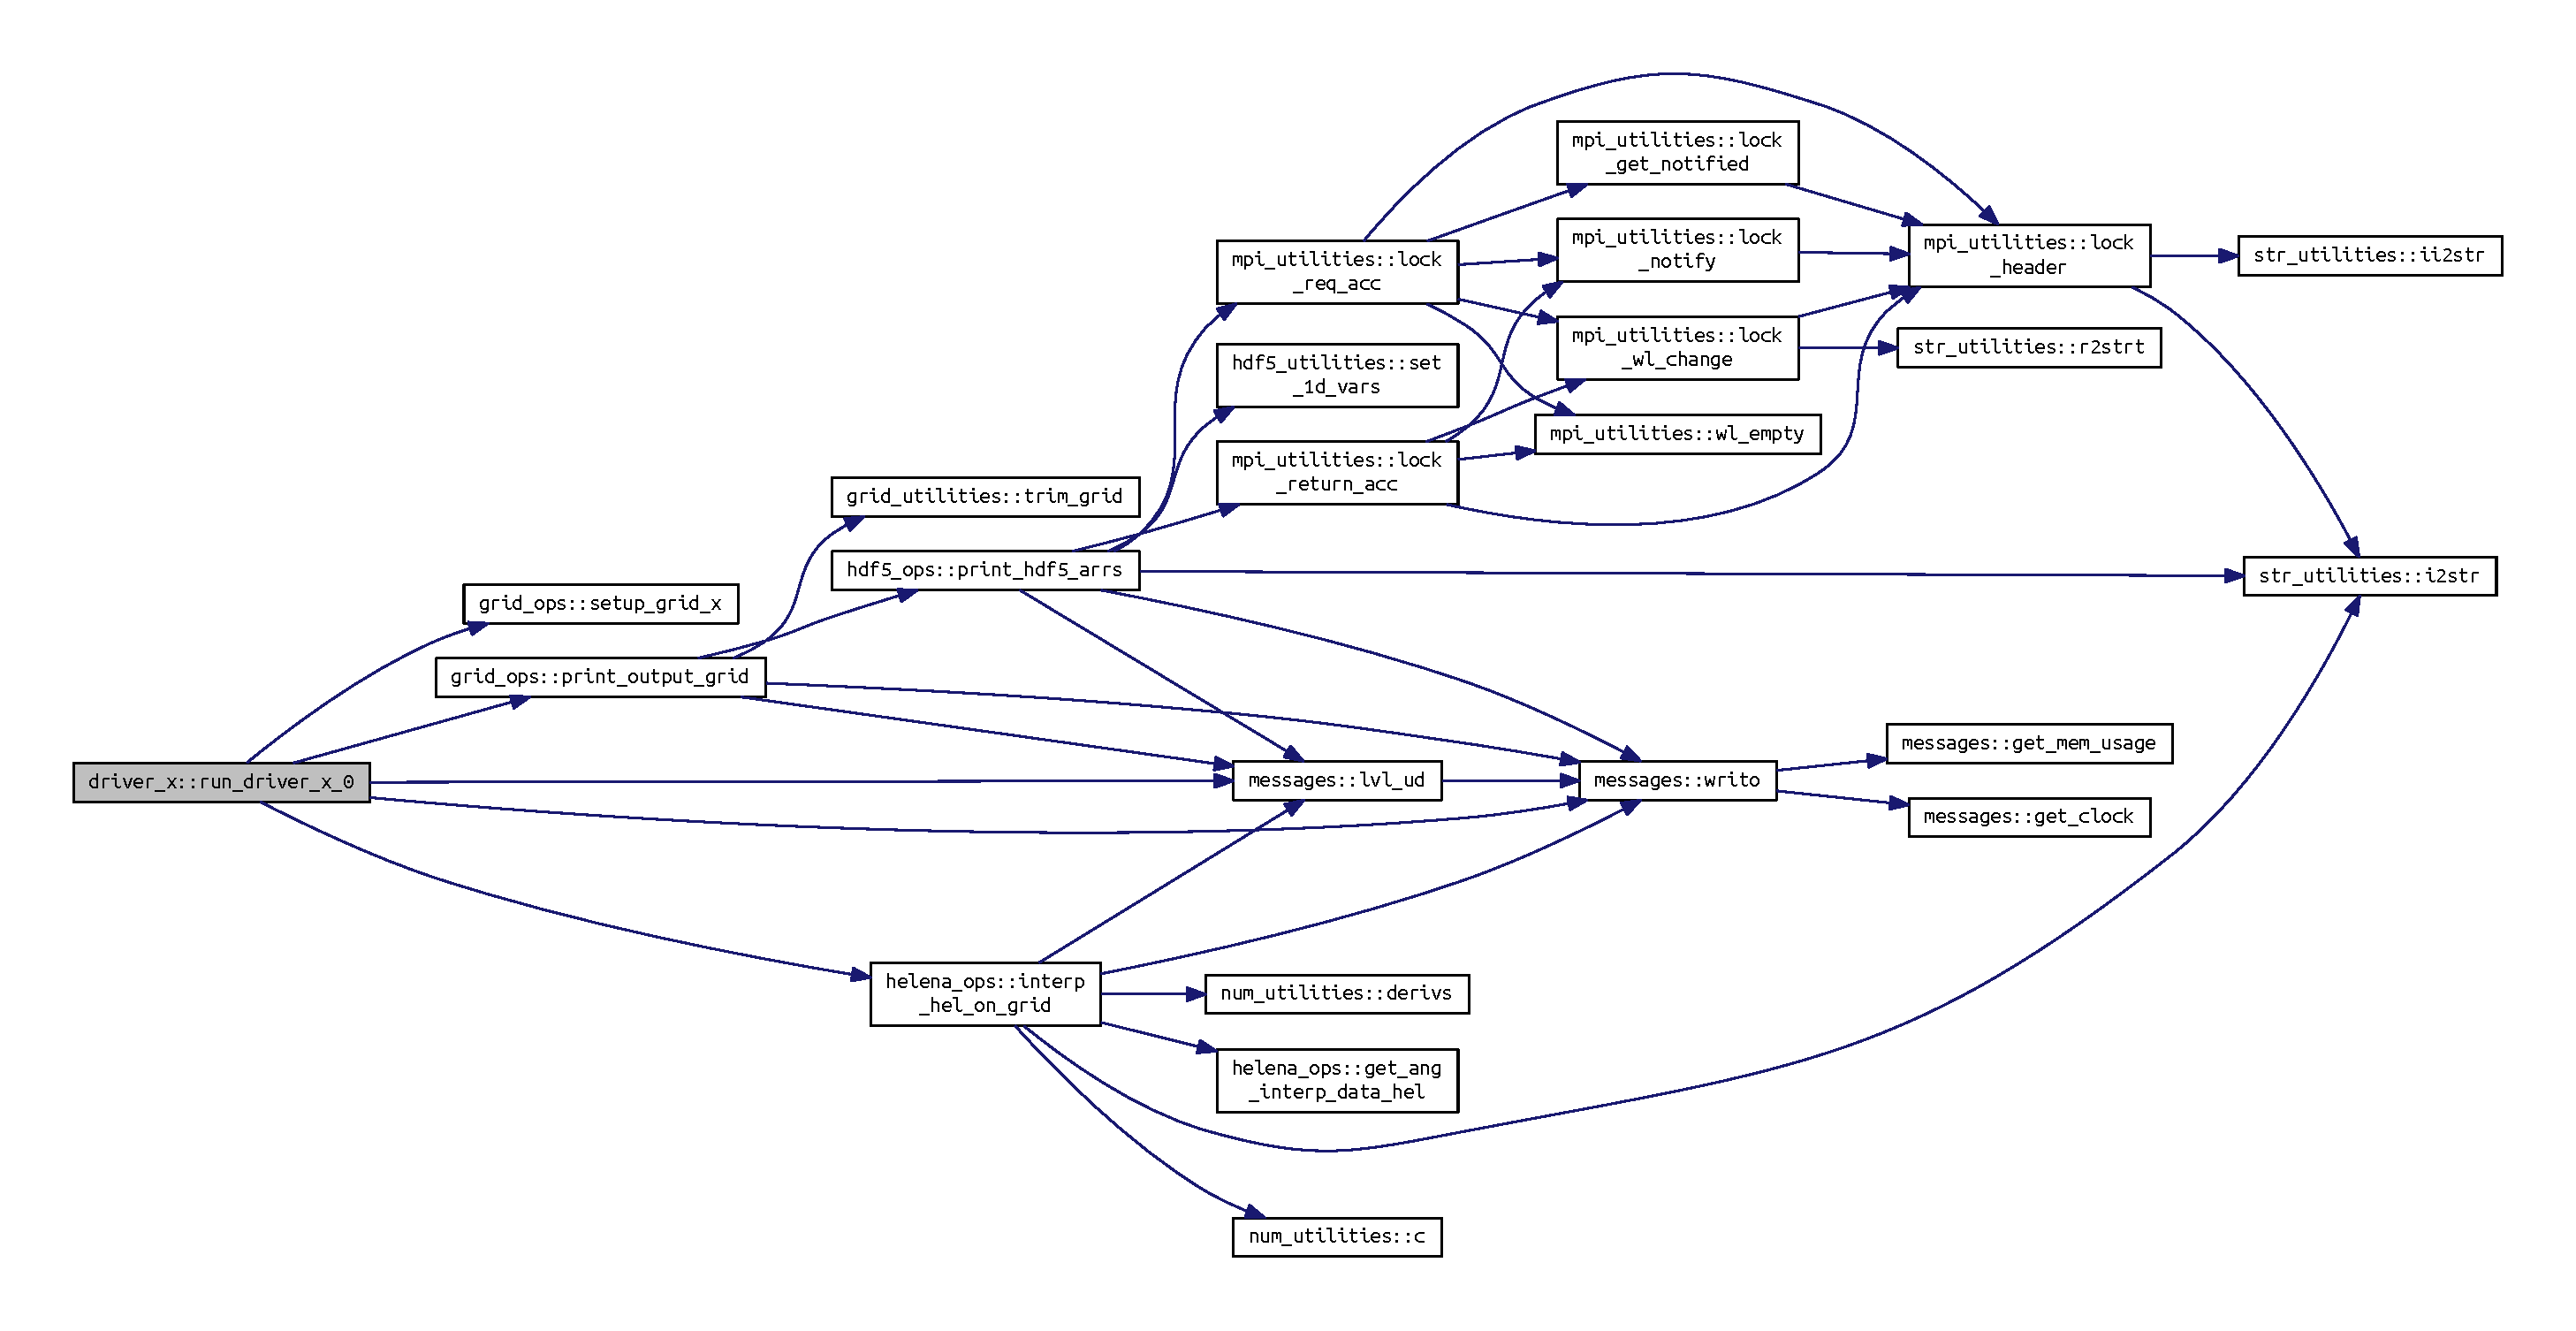
\includegraphics[width=350pt]{namespacedriver__x_a2b82a9bc6c0f4af9f3468d03fedc008e_cgraph}
\end{center}
\end{figure}
Here is the caller graph for this function\+:
\nopagebreak
\begin{figure}[H]
\begin{center}
\leavevmode
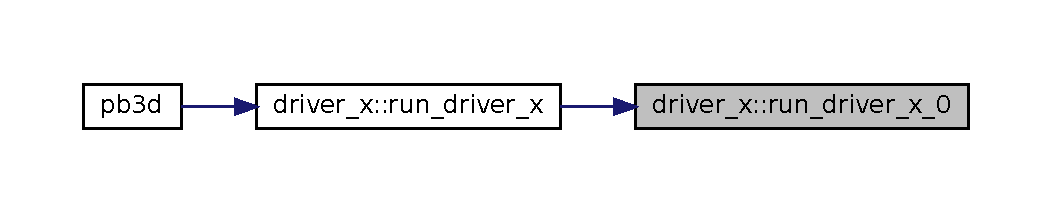
\includegraphics[width=350pt]{namespacedriver__x_a2b82a9bc6c0f4af9f3468d03fedc008e_icgraph}
\end{center}
\end{figure}
\mbox{\Hypertarget{namespacedriver__x_a454779cefa6da3714d32eedcec0ef7de}\label{namespacedriver__x_a454779cefa6da3714d32eedcec0ef7de}} 
\index{driver\+\_\+x@{driver\+\_\+x}!run\+\_\+driver\+\_\+x\+\_\+1@{run\+\_\+driver\+\_\+x\+\_\+1}}
\index{run\+\_\+driver\+\_\+x\+\_\+1@{run\+\_\+driver\+\_\+x\+\_\+1}!driver\+\_\+x@{driver\+\_\+x}}
\subsubsection{\texorpdfstring{run\+\_\+driver\+\_\+x\+\_\+1()}{run\_driver\_x\_1()}}
{\footnotesize\ttfamily integer function driver\+\_\+x\+::run\+\_\+driver\+\_\+x\+\_\+1 (\begin{DoxyParamCaption}\item[{type(grid\+\_\+type), intent(in)}]{grid\+\_\+eq,  }\item[{type(grid\+\_\+type), intent(in)}]{grid\+\_\+X,  }\item[{type(eq\+\_\+1\+\_\+type), intent(in)}]{eq\+\_\+1,  }\item[{type(eq\+\_\+2\+\_\+type), intent(in)}]{eq\+\_\+2,  }\item[{type(x\+\_\+1\+\_\+type), intent(inout)}]{X\+\_\+1 }\end{DoxyParamCaption})}



Definition at line 335 of file driver\+\_\+\+X.\+f90.

Here is the call graph for this function\+:
\nopagebreak
\begin{figure}[H]
\begin{center}
\leavevmode
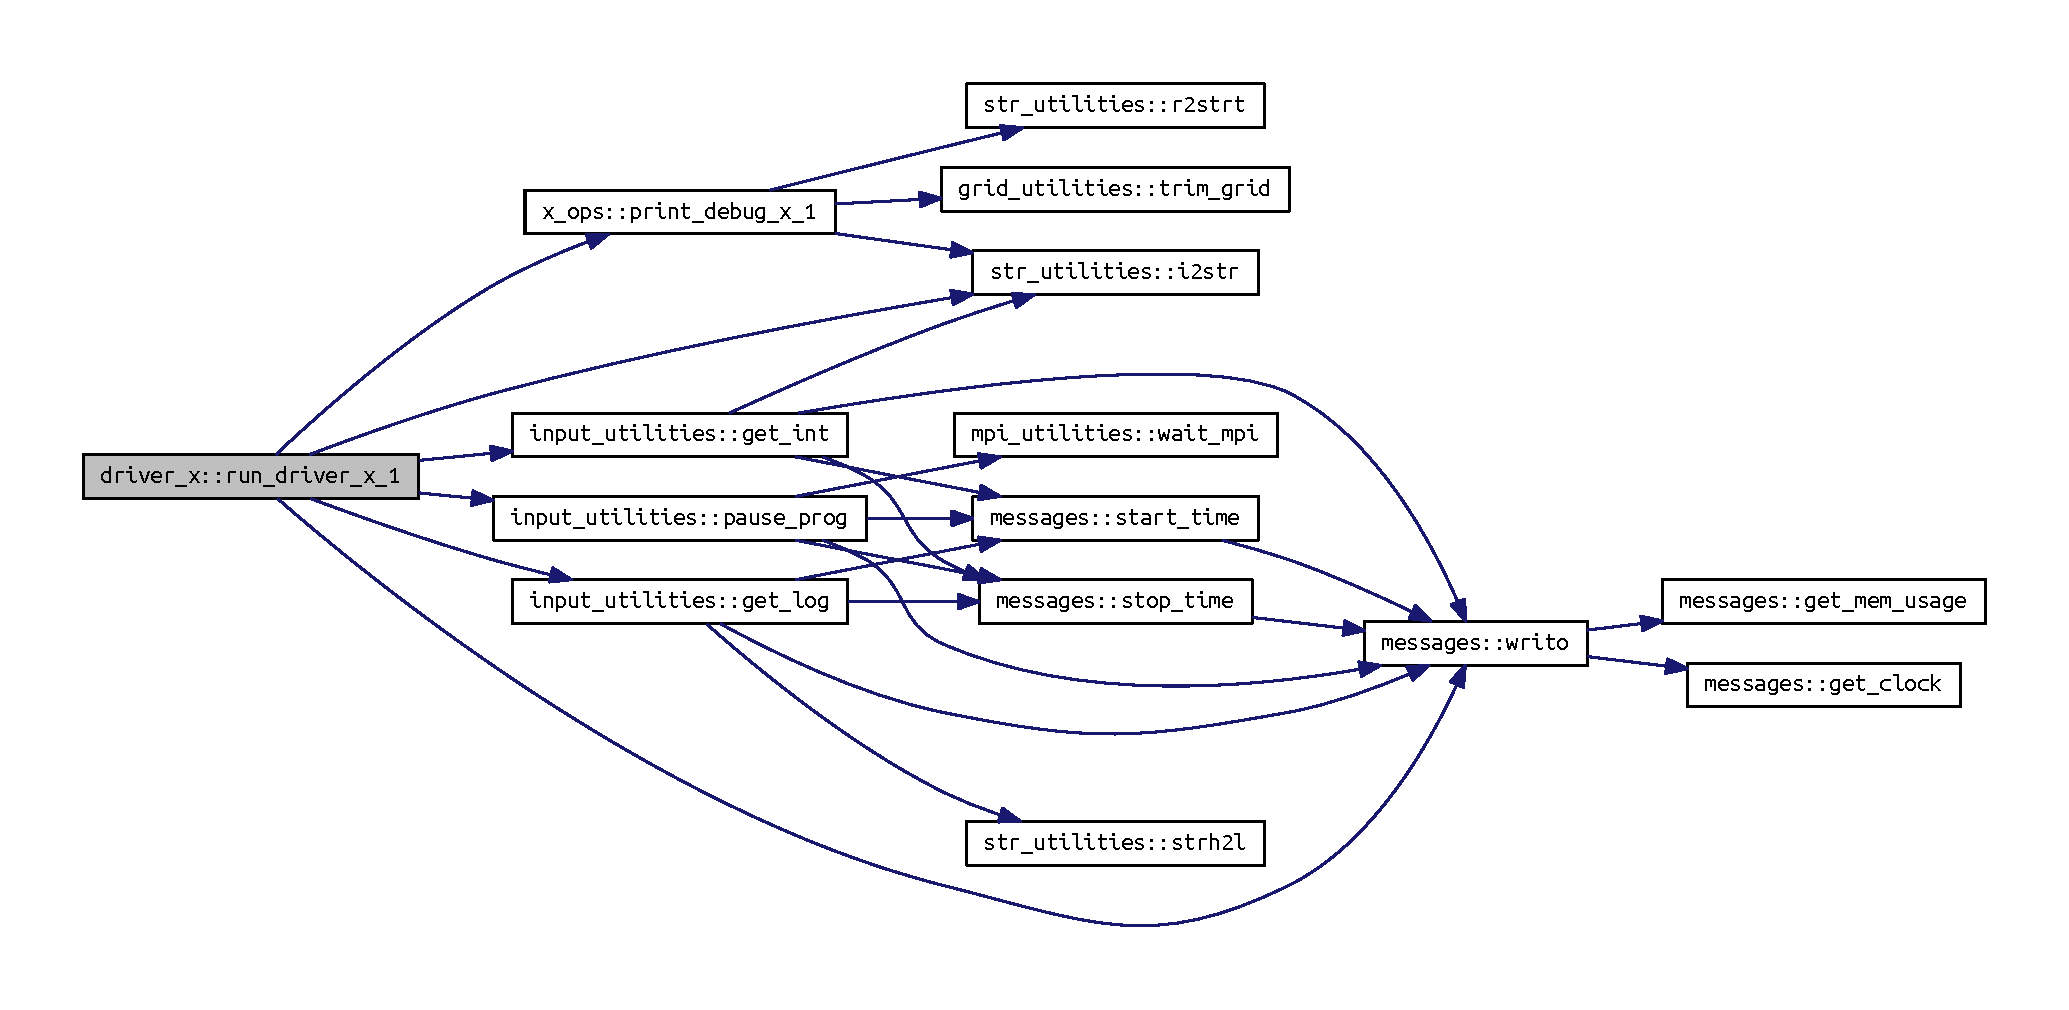
\includegraphics[width=350pt]{namespacedriver__x_a454779cefa6da3714d32eedcec0ef7de_cgraph}
\end{center}
\end{figure}
Here is the caller graph for this function\+:
\nopagebreak
\begin{figure}[H]
\begin{center}
\leavevmode
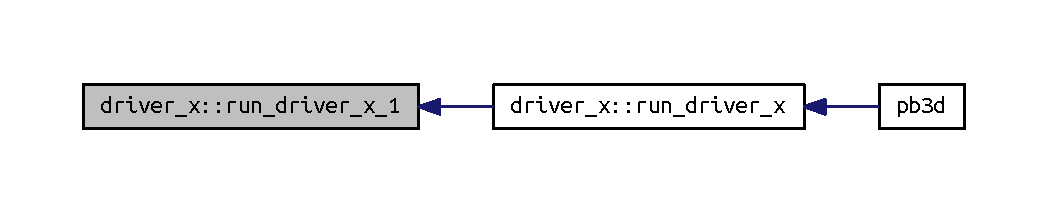
\includegraphics[width=350pt]{namespacedriver__x_a454779cefa6da3714d32eedcec0ef7de_icgraph}
\end{center}
\end{figure}
\mbox{\Hypertarget{namespacedriver__x_ad3924b3d66f336f0a9a9559eafffec8e}\label{namespacedriver__x_ad3924b3d66f336f0a9a9559eafffec8e}} 
\index{driver\+\_\+x@{driver\+\_\+x}!run\+\_\+driver\+\_\+x\+\_\+2@{run\+\_\+driver\+\_\+x\+\_\+2}}
\index{run\+\_\+driver\+\_\+x\+\_\+2@{run\+\_\+driver\+\_\+x\+\_\+2}!driver\+\_\+x@{driver\+\_\+x}}
\subsubsection{\texorpdfstring{run\+\_\+driver\+\_\+x\+\_\+2()}{run\_driver\_x\_2()}}
{\footnotesize\ttfamily integer function driver\+\_\+x\+::run\+\_\+driver\+\_\+x\+\_\+2 (\begin{DoxyParamCaption}\item[{type(grid\+\_\+type), intent(in), pointer}]{grid\+\_\+eq\+\_\+B,  }\item[{type(grid\+\_\+type), intent(in), target}]{grid\+\_\+X,  }\item[{type(grid\+\_\+type), intent(in), pointer}]{grid\+\_\+\+X\+\_\+B,  }\item[{type(eq\+\_\+1\+\_\+type), intent(in)}]{eq\+\_\+1,  }\item[{type(eq\+\_\+2\+\_\+type), intent(in), pointer}]{eq\+\_\+2\+\_\+B,  }\item[{type(x\+\_\+1\+\_\+type), intent(in)}]{X\+\_\+1,  }\item[{type(x\+\_\+2\+\_\+type), intent(inout)}]{X\+\_\+2\+\_\+int }\end{DoxyParamCaption})}



Definition at line 546 of file driver\+\_\+\+X.\+f90.

Here is the call graph for this function\+:
\nopagebreak
\begin{figure}[H]
\begin{center}
\leavevmode
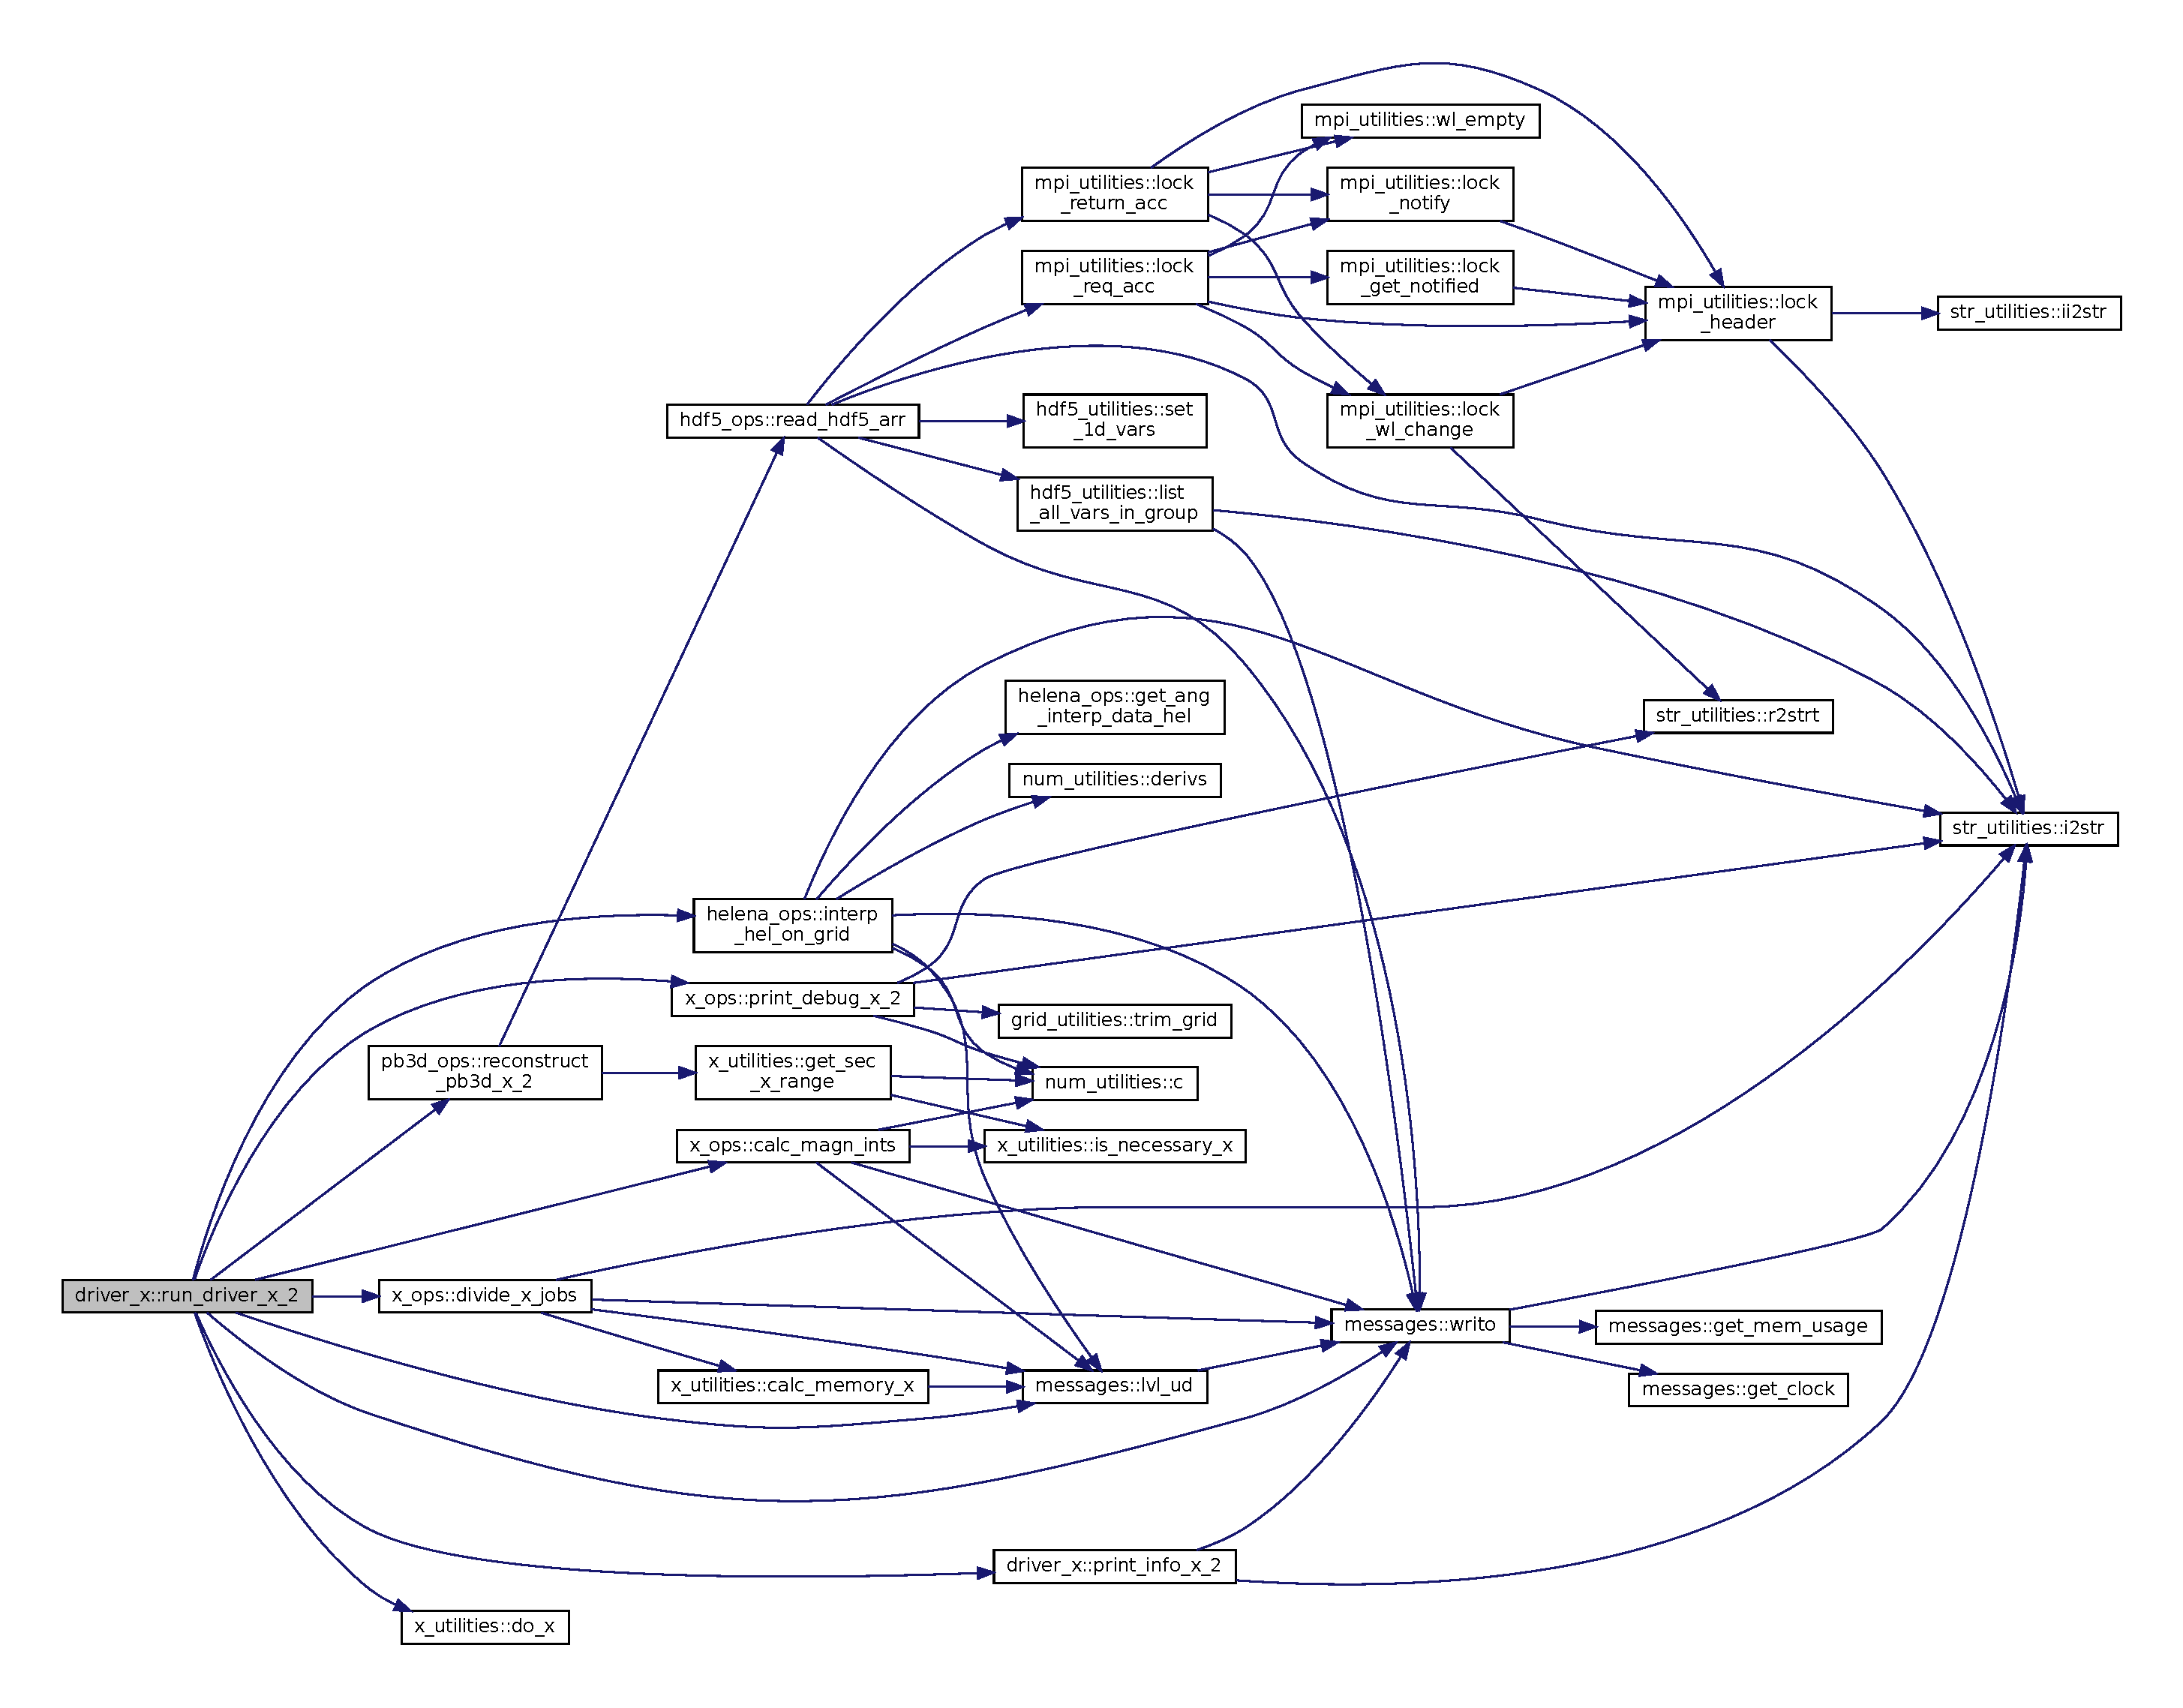
\includegraphics[width=350pt]{namespacedriver__x_ad3924b3d66f336f0a9a9559eafffec8e_cgraph}
\end{center}
\end{figure}
Here is the caller graph for this function\+:
\nopagebreak
\begin{figure}[H]
\begin{center}
\leavevmode
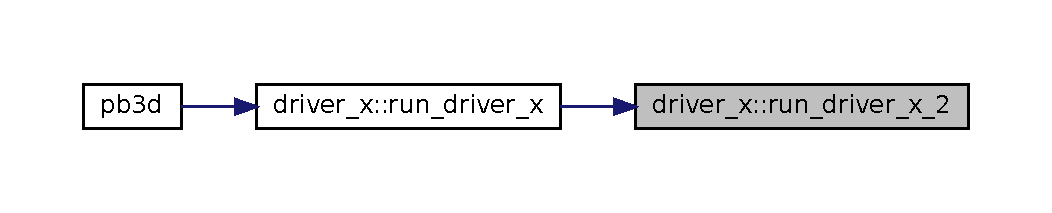
\includegraphics[width=350pt]{namespacedriver__x_ad3924b3d66f336f0a9a9559eafffec8e_icgraph}
\end{center}
\end{figure}

\hypertarget{namespacedtorh}{}\doxysection{dtorh Module Reference}
\label{namespacedtorh}\index{dtorh@{dtorh}}


Calculation of toroidal functions $P_{n-1/2}^m \left(z\right)$ and $Q_{n-1/2}^m \left(z\right)$.  


\doxysubsection*{Functions/\+Subroutines}
\begin{DoxyCompactItemize}
\item 
integer function, public \mbox{\hyperlink{namespacedtorh_af3f58b6705da916bfbaf7cc4ea05f610}{dtorh1}} (z, m, nmax, pl, ql, newn, mode, ipre)
\begin{DoxyCompactList}\small\item\em Calculates toroidal harmonics of a fixed order {\ttfamily m} and degrees up to {\ttfamily nmax}. \end{DoxyCompactList}\end{DoxyCompactItemize}


\doxysubsection{Detailed Description}
Calculation of toroidal functions $P_{n-1/2}^m \left(z\right)$ and $Q_{n-1/2}^m \left(z\right)$. 

\begin{DoxyNote}{Note}
Copied and adapted from the D\+T\+O\+R\+H1 routine by Segura and Gil \cite{Segura2000} . 
\end{DoxyNote}


\doxysubsection{Function/\+Subroutine Documentation}
\mbox{\Hypertarget{namespacedtorh_af3f58b6705da916bfbaf7cc4ea05f610}\label{namespacedtorh_af3f58b6705da916bfbaf7cc4ea05f610}} 
\index{dtorh@{dtorh}!dtorh1@{dtorh1}}
\index{dtorh1@{dtorh1}!dtorh@{dtorh}}
\doxysubsubsection{\texorpdfstring{dtorh1()}{dtorh1()}}
{\footnotesize\ttfamily integer function, public dtorh\+::dtorh1 (\begin{DoxyParamCaption}\item[{real(dp), intent(in)}]{z,  }\item[{integer, intent(in)}]{m,  }\item[{integer, intent(in)}]{nmax,  }\item[{real(dp), dimension(0\+:nmax), intent(inout)}]{pl,  }\item[{real(dp), dimension(0\+:nmax), intent(inout)}]{ql,  }\item[{integer, intent(inout)}]{newn,  }\item[{integer, intent(in), optional}]{mode,  }\item[{integer, intent(in), optional}]{ipre }\end{DoxyParamCaption})}



Calculates toroidal harmonics of a fixed order {\ttfamily m} and degrees up to {\ttfamily nmax}. 

Optionally, the {\ttfamily mode} can be specified to be different from 0 \mbox{[}default\mbox{]}
\begin{DoxyItemize}
\item if {\ttfamily mode=1}\+:
\begin{DoxyItemize}
\item The set of functions evaluated is\+: \[\frac{P_{n-1/2}^m \left(z\right)}{\Gamma(m+1/2)} \ ,\quad \frac{Q_{n-1/2}^m \left(z\right)}{\Gamma(m+1/2)},\] which are respectively stored in the arrays {\ttfamily pl(n)}, {\ttfamily ql(n)}.
\item newn refers to this new set of functions.
\item Note 1. and note 2. also apply in this case.
\end{DoxyItemize}
\item if {\ttfamily mode=2}\+:
\begin{DoxyItemize}
\item The code performs as for mode 1, but the restriction $ z<20 $.
\item For the evaluation of the continued fraction is not considered.
\end{DoxyItemize}
\end{DoxyItemize}

Also, the parameter {\ttfamily ipre} can be used to select a different precision\+:
\begin{DoxyItemize}
\item For {\ttfamily ipre=1}, the precision is $10^{-12}$, taking $\epsilon<10^{-12}$
\item For {\ttfamily ipre=2}, the precision is $10^{-8}$, taking $\epsilon<10^{-8}$
\end{DoxyItemize}

where $\epsilon$ controls the accuracy.

\begin{DoxyWarning}{Warning}
Use {\ttfamily mode} 2 only if high {\ttfamily m} \textquotesingle{}s for $z>20$ are required. The evaluation of the cf may fail to converge for too high {\ttfamily z} \textquotesingle{}s.
\end{DoxyWarning}
\begin{DoxyNote}{Note}

\begin{DoxyEnumerate}
\item For a precision of $10^{-12}$, if $z>5$ and $z/m>0.22$, the code uses a series expansion for {\ttfamily pl(0)}.~\newline
 When $z<20$ and $z/m<0.22$ a continued fraction is applied.
\item For a precision of $10^{-8}$, if $z>5$ and $z/m>0.12$, the code uses a series expansion for {\ttfamily pl(0)}.~\newline
 When $z<20$ and $z/m<0.12$ a continued fraction is applied.
\end{DoxyEnumerate}
\end{DoxyNote}
\begin{DoxyReturn}{Returns}
ierr 
\end{DoxyReturn}

\begin{DoxyParams}[1]{Parameters}
\mbox{\texttt{ in}}  & {\em z} & (real) point at which toroidal harmonics are evaluated \\
\hline
\mbox{\texttt{ in}}  & {\em m} & order of toroidal harmonics ({\ttfamily m$>$0}) \\
\hline
\mbox{\texttt{ in}}  & {\em nmax} & maximum degree of toroidal harmonics ({\ttfamily nmax$>$0}) \\
\hline
\mbox{\texttt{ in,out}}  & {\em pl} & toroidal harmonics of first kind $P_{n-1/2}^m\left(z\right)$ \\
\hline
\mbox{\texttt{ in,out}}  & {\em ql} & toroidal harmonics of second kind $Q_{n-1/2}^m\left(z\right)$ \\
\hline
\mbox{\texttt{ in,out}}  & {\em newn} & maximum order of functions calculated when {\ttfamily  pl(nmax+1)$>$1/tiny } with {\ttfamily tiny=} $10^{-290}$ \\
\hline
\mbox{\texttt{ in}}  & {\em mode} & mode that controls output \\
\hline
\mbox{\texttt{ in}}  & {\em ipre} & precision \\
\hline
\end{DoxyParams}


Definition at line 75 of file dtorh.\+f90.

Here is the call graph for this function\+:\nopagebreak
\begin{figure}[H]
\begin{center}
\leavevmode
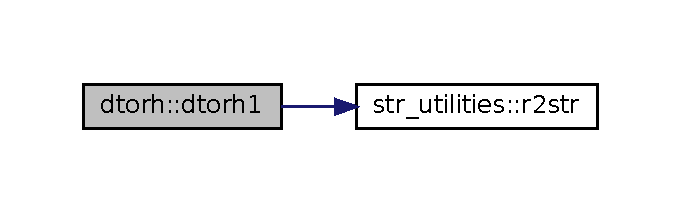
\includegraphics[width=327pt]{namespacedtorh_af3f58b6705da916bfbaf7cc4ea05f610_cgraph}
\end{center}
\end{figure}
Here is the caller graph for this function\+:\nopagebreak
\begin{figure}[H]
\begin{center}
\leavevmode
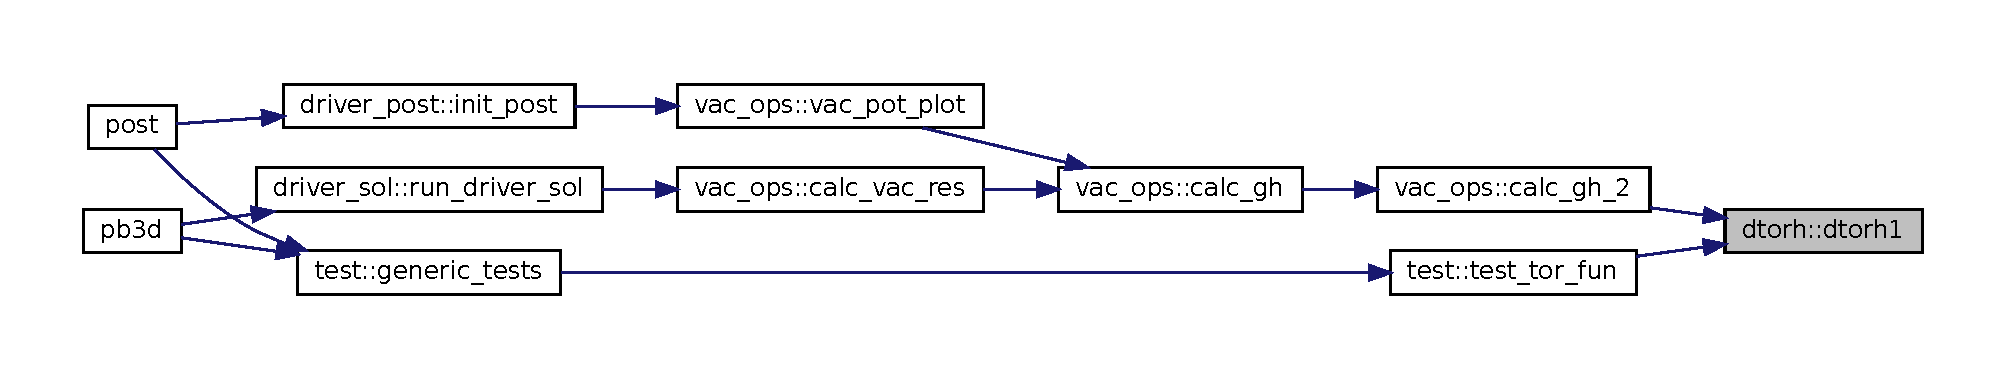
\includegraphics[width=350pt]{namespacedtorh_af3f58b6705da916bfbaf7cc4ea05f610_icgraph}
\end{center}
\end{figure}

\hypertarget{namespaceeq__ops}{}\section{eq\+\_\+ops Module Reference}
\label{namespaceeq__ops}\index{eq\+\_\+ops@{eq\+\_\+ops}}


Operations on the equilibrium variables.  


\subsection*{Interfaces and Types}
\begin{DoxyCompactItemize}
\item 
interface \hyperlink{interfaceeq__ops_1_1calc__eq}{calc\+\_\+eq}
\begin{DoxyCompactList}\small\item\em Calculate the equilibrium quantities on a grid determined by straight field lines. \end{DoxyCompactList}\item 
interface \hyperlink{interfaceeq__ops_1_1calc__g__c}{calc\+\_\+g\+\_\+c}
\begin{DoxyCompactList}\small\item\em Calculate the lower metric elements in the C(ylindrical) coordinate system. \end{DoxyCompactList}\item 
interface \hyperlink{interfaceeq__ops_1_1calc__g__f}{calc\+\_\+g\+\_\+f}
\begin{DoxyCompactList}\small\item\em Calculate the metric coefficients in the F(lux) coordinate system. \end{DoxyCompactList}\item 
interface \hyperlink{interfaceeq__ops_1_1calc__g__h}{calc\+\_\+g\+\_\+h}
\begin{DoxyCompactList}\small\item\em Calculate the lower metric coefficients in the equilibrium H(\+E\+L\+E\+N\+A) coordinate system. \end{DoxyCompactList}\item 
interface \hyperlink{interfaceeq__ops_1_1calc__g__v}{calc\+\_\+g\+\_\+v}
\begin{DoxyCompactList}\small\item\em Calculate the lower metric coefficients in the equilibrium V(\+M\+E\+C) coordinate system. \end{DoxyCompactList}\item 
interface \hyperlink{interfaceeq__ops_1_1calc__jac__f}{calc\+\_\+jac\+\_\+f}
\begin{DoxyCompactList}\small\item\em Calculate $\mathcal{J}_\text{F}$, the jacobian in Flux coordinates. \end{DoxyCompactList}\item 
interface \hyperlink{interfaceeq__ops_1_1calc__jac__h}{calc\+\_\+jac\+\_\+h}
\begin{DoxyCompactList}\small\item\em Calculate $\mathcal{J}_\text{H}$, the jacobian in H\+E\+L\+E\+NA coordinates. \end{DoxyCompactList}\item 
interface \hyperlink{interfaceeq__ops_1_1calc__jac__v}{calc\+\_\+jac\+\_\+v}
\begin{DoxyCompactList}\small\item\em Calculate $\mathcal{J}_\text{V}$, the jacobian in V(\+M\+E\+C) coordinates. \end{DoxyCompactList}\item 
interface \hyperlink{interfaceeq__ops_1_1calc__rzl}{calc\+\_\+rzl}
\begin{DoxyCompactList}\small\item\em Calculate $R$, $Z$ \& $\lambda$ and derivatives in V\+M\+EC coordinates. \end{DoxyCompactList}\item 
interface \hyperlink{interfaceeq__ops_1_1calc__t__hf}{calc\+\_\+t\+\_\+hf}
\begin{DoxyCompactList}\small\item\em Calculate $\overline{\text{T}}_\text{H}^\text{F}$, the transformation matrix between H(\+E\+L\+E\+N\+A) and F(lux) coordinate systems. \end{DoxyCompactList}\item 
interface \hyperlink{interfaceeq__ops_1_1calc__t__vc}{calc\+\_\+t\+\_\+vc}
\begin{DoxyCompactList}\small\item\em Calculate $\overline{\text{T}}_\text{C}^\text{V}$, the transformation matrix between C(ylindrical) and V(mec) coordinate system. \end{DoxyCompactList}\item 
interface \hyperlink{interfaceeq__ops_1_1calc__t__vf}{calc\+\_\+t\+\_\+vf}
\begin{DoxyCompactList}\small\item\em Calculate $\overline{\text{T}}_\text{V}^\text{F}$, the transformation matrix between V(\+M\+E\+C) and F(lux) coordinate systems. \end{DoxyCompactList}\item 
interface \hyperlink{interfaceeq__ops_1_1print__output__eq}{print\+\_\+output\+\_\+eq}
\begin{DoxyCompactList}\small\item\em Print equilibrium quantities to an output file\+: \end{DoxyCompactList}\item 
interface \hyperlink{interfaceeq__ops_1_1redistribute__output__eq}{redistribute\+\_\+output\+\_\+eq}
\begin{DoxyCompactList}\small\item\em Redistribute the equilibrium variables, but only the Flux variables are saved. \end{DoxyCompactList}\end{DoxyCompactItemize}
\subsection*{Functions/\+Subroutines}
\begin{DoxyCompactItemize}
\item 
integer function \hyperlink{namespaceeq__ops_a9addef683b3d4a8c587510e4c994ec61}{create\+\_\+vmec\+\_\+input} (grid\+\_\+eq, eq\+\_\+1)
\begin{DoxyCompactList}\small\item\em Creates a V\+M\+EC input file. \end{DoxyCompactList}\item 
integer function, public \hyperlink{namespaceeq__ops_af0effe20188d46a44680c2648e4572e9}{flux\+\_\+q\+\_\+plot} (grid\+\_\+eq, eq)
\begin{DoxyCompactList}\small\item\em Plots the flux quantities in the solution grid. \end{DoxyCompactList}\item 
integer function, public \hyperlink{namespaceeq__ops_a087e08ce6d8ad381b5bac8fc51148d50}{calc\+\_\+derived\+\_\+q} (grid\+\_\+eq, eq\+\_\+1, eq\+\_\+2)
\begin{DoxyCompactList}\small\item\em Calculates derived equilibrium quantities system. \end{DoxyCompactList}\item 
integer function, public \hyperlink{namespaceeq__ops_a7cd38586e386e1bc684a327ebcc4c1de}{calc\+\_\+normalization\+\_\+const} ()
\begin{DoxyCompactList}\small\item\em Sets up normalization constants. \end{DoxyCompactList}\item 
subroutine, public \hyperlink{namespaceeq__ops_a1b4c764da73624722d7e76498a2b80a9}{normalize\+\_\+input} ()
\begin{DoxyCompactList}\small\item\em Normalize input quantities. \end{DoxyCompactList}\item 
integer function, public \hyperlink{namespaceeq__ops_a73a8c3cea1e8a636b4978bc626e0fab0}{b\+\_\+plot} (grid\+\_\+eq, eq\+\_\+1, eq\+\_\+2, rich\+\_\+lvl, plot\+\_\+fluxes, X\+YZ)
\begin{DoxyCompactList}\small\item\em Plots the magnetic fields. \end{DoxyCompactList}\item 
integer function, public \hyperlink{namespaceeq__ops_afabdf28e5c26ceb87e6eb8cf3809919d}{j\+\_\+plot} (grid\+\_\+eq, eq\+\_\+1, eq\+\_\+2, rich\+\_\+lvl, plot\+\_\+fluxes, X\+YZ)
\begin{DoxyCompactList}\small\item\em Plots the current. \end{DoxyCompactList}\item 
integer function, public \hyperlink{namespaceeq__ops_ad173efd111cb85c11bc2bc78a7555096}{kappa\+\_\+plot} (grid\+\_\+eq, eq\+\_\+1, eq\+\_\+2, rich\+\_\+lvl, X\+YZ)
\begin{DoxyCompactList}\small\item\em Plots the curvature. \end{DoxyCompactList}\item 
integer function, public \hyperlink{namespaceeq__ops_ac0a79893900631d25b170be0abd2c131}{delta\+\_\+r\+\_\+plot} (grid\+\_\+eq, eq\+\_\+1, eq\+\_\+2, X\+YZ, rich\+\_\+lvl)
\begin{DoxyCompactList}\small\item\em Plots {\bfseries H\+A\+LF} of the change in the position vectors for 2 different toroidal positions, which can correspond to a ripple. \end{DoxyCompactList}\item 
integer function, public \hyperlink{namespaceeq__ops_a8fae749abe55865d8135fef536a8e8f1}{divide\+\_\+eq\+\_\+jobs} (n\+\_\+par\+\_\+X, arr\+\_\+size, n\+\_\+div, n\+\_\+div\+\_\+max, n\+\_\+par\+\_\+\+X\+\_\+base, range\+\_\+name)
\begin{DoxyCompactList}\small\item\em Divides the equilibrium jobs. \end{DoxyCompactList}\item 
integer function, public \hyperlink{namespaceeq__ops_a4e20b8725fce149449f83754244dc84e}{calc\+\_\+eq\+\_\+jobs\+\_\+lims} (n\+\_\+par\+\_\+X, n\+\_\+div)
\begin{DoxyCompactList}\small\item\em Calculate {\ttfamily eq\+\_\+jobs\+\_\+lims}. \end{DoxyCompactList}\item 
integer function \hyperlink{namespaceeq__ops_a1f5049c3e309fa23ee46fd116c9344f1}{test\+\_\+t\+\_\+ef} (grid\+\_\+eq, eq\+\_\+1, eq\+\_\+2)
\begin{DoxyCompactList}\small\item\em See if {\ttfamily T\+\_\+\+EF} it complies with the theory of \cite{Weyens3D}. \end{DoxyCompactList}\item 
integer function \hyperlink{namespaceeq__ops_a003df1e1ab90dc6f586c3eed3dd067e8}{test\+\_\+d12h\+\_\+h} (grid\+\_\+eq, eq)
\begin{DoxyCompactList}\small\item\em Tests whether $ \frac{\partial^2}{\partial u_i \partial u_j} h_\text{H} $ is calculated correctly. \end{DoxyCompactList}\item 
integer function \hyperlink{namespaceeq__ops_a05dcd4803b9c7845d3353614c9630c23}{test\+\_\+jac\+\_\+f} (grid\+\_\+eq, eq\+\_\+1, eq\+\_\+2)
\begin{DoxyCompactList}\small\item\em Performs tests on $ \mathcal{J}_\text{F}$. \end{DoxyCompactList}\item 
integer function \hyperlink{namespaceeq__ops_a9811c83477d9d85f7401fd7957a590fc}{test\+\_\+g\+\_\+v} (grid\+\_\+eq, eq)
\begin{DoxyCompactList}\small\item\em Tests whether $g_\text{V}$ is calculated correctly. \end{DoxyCompactList}\item 
integer function \hyperlink{namespaceeq__ops_aef40d04e93f6a96576f8fe893fb086f8}{test\+\_\+jac\+\_\+v} (grid\+\_\+eq, eq)
\begin{DoxyCompactList}\small\item\em Tests whether $\mathcal{J}_\text{V}$ is calculated correctly. \end{DoxyCompactList}\item 
integer function \hyperlink{namespaceeq__ops_a8082c12510696bd8ffdd0deef41860c2}{test\+\_\+b\+\_\+f} (grid\+\_\+eq, eq\+\_\+1, eq\+\_\+2)
\begin{DoxyCompactList}\small\item\em Tests whether $\vec{B}_\text{F}$ is calculated correctly. \end{DoxyCompactList}\item 
integer function \hyperlink{namespaceeq__ops_a38b723f6ed5d2e2772c9c3ad14d5ffd4}{test\+\_\+p} (grid\+\_\+eq, eq\+\_\+1, eq\+\_\+2)
\begin{DoxyCompactList}\small\item\em Performs tests on pressure balance. \end{DoxyCompactList}\end{DoxyCompactItemize}
\subsection*{Variables}
\begin{DoxyCompactItemize}
\item 
logical, public \hyperlink{namespaceeq__ops_a1b6609a8d8b427d9133bf323e732f209}{debug\+\_\+calc\+\_\+derived\+\_\+q} = .false.
\begin{DoxyCompactList}\small\item\em plot debug information for \hyperlink{namespaceeq__ops_a087e08ce6d8ad381b5bac8fc51148d50}{calc\+\_\+derived\+\_\+q()} \end{DoxyCompactList}\item 
logical, public \hyperlink{namespaceeq__ops_a45ba7f46fd439bbd73edfd1fd548b58e}{debug\+\_\+j\+\_\+plot} = .false.
\begin{DoxyCompactList}\small\item\em plot debug information for \hyperlink{namespaceeq__ops_afabdf28e5c26ceb87e6eb8cf3809919d}{j\+\_\+plot()} \end{DoxyCompactList}\item 
logical, public \hyperlink{namespaceeq__ops_a07ca60790a262e20bc8632be1530970a}{debug\+\_\+create\+\_\+vmec\+\_\+input} = .false.
\begin{DoxyCompactList}\small\item\em plot debug information for \hyperlink{namespaceeq__ops_a9addef683b3d4a8c587510e4c994ec61}{create\+\_\+vmec\+\_\+input()} \end{DoxyCompactList}\end{DoxyCompactItemize}


\subsection{Detailed Description}
Operations on the equilibrium variables. 

\subsection{Function/\+Subroutine Documentation}
\mbox{\Hypertarget{namespaceeq__ops_a73a8c3cea1e8a636b4978bc626e0fab0}\label{namespaceeq__ops_a73a8c3cea1e8a636b4978bc626e0fab0}} 
\index{eq\+\_\+ops@{eq\+\_\+ops}!b\+\_\+plot@{b\+\_\+plot}}
\index{b\+\_\+plot@{b\+\_\+plot}!eq\+\_\+ops@{eq\+\_\+ops}}
\subsubsection{\texorpdfstring{b\+\_\+plot()}{b\_plot()}}
{\footnotesize\ttfamily integer function, public eq\+\_\+ops\+::b\+\_\+plot (\begin{DoxyParamCaption}\item[{type(\hyperlink{structgrid__vars_1_1grid__type}{grid\+\_\+type}), intent(inout)}]{grid\+\_\+eq,  }\item[{type(\hyperlink{structeq__vars_1_1eq__1__type}{eq\+\_\+1\+\_\+type}), intent(in)}]{eq\+\_\+1,  }\item[{type(\hyperlink{structeq__vars_1_1eq__2__type}{eq\+\_\+2\+\_\+type}), intent(in)}]{eq\+\_\+2,  }\item[{integer, intent(in), optional}]{rich\+\_\+lvl,  }\item[{logical, intent(in), optional}]{plot\+\_\+fluxes,  }\item[{real(dp), dimension(\+:,\+:,\+:,\+:), intent(in), optional}]{X\+YZ }\end{DoxyParamCaption})}



Plots the magnetic fields. 

If multiple equilibrium parallel jobs, every job does its piece, and the results are joined automatically by plot\+\_\+\+H\+D\+F5.

The outputs are given in contra-\/ and covariant components and magnitude in multiple coordinate systems, as indicated in \hyperlink{namespacegrid__utilities_ad3d9386b9abcb1a7e17369a1b3a3750d}{calc\+\_\+vec\+\_\+comp()}.

The starting point is the fact that the magnetic field is given by \[\vec{B} = \frac{\vec{e}_{\theta}}{\mathcal{J}}, \] in F coordinates. The F covariant components are therefore given by \[B_i = \frac{g_{i3}}{\mathcal{J}} = \frac{\vec{e}_i \cdot \vec{e}_3}{\mathcal{J}}, \] and the only non-\/vanishing contravariant component is \[B^3 = \frac{1}{\mathcal{J}}. \]

These are then all be transformed to the other coordinate systems.

\begin{DoxyNote}{Note}

\begin{DoxyEnumerate}
\item Vector plots for different Richardson levels can be combined to show the total grid by just plotting them all individually.
\item The metric factors and transformation matrices have to be allocated.
\end{DoxyEnumerate}
\end{DoxyNote}
\begin{DoxyReturn}{Returns}
ierr
\end{DoxyReturn}

\begin{DoxyParams}[1]{Parameters}
\mbox{\tt in,out}  & {\em grid\+\_\+eq} & equilibrium grid\\
\hline
\mbox{\tt in}  & {\em eq\+\_\+1} & flux equilibrium variables\\
\hline
\mbox{\tt in}  & {\em eq\+\_\+2} & metric equilibrium variables\\
\hline
\mbox{\tt in}  & {\em rich\+\_\+lvl} & Richardson level\\
\hline
\mbox{\tt in}  & {\em plot\+\_\+fluxes} & plot the fluxes\\
\hline
\mbox{\tt in}  & {\em xyz} & X, Y and Z of grid \\
\hline
\end{DoxyParams}


Definition at line 5054 of file eq\+\_\+ops.\+f90.

Here is the call graph for this function\+:\nopagebreak
\begin{figure}[H]
\begin{center}
\leavevmode
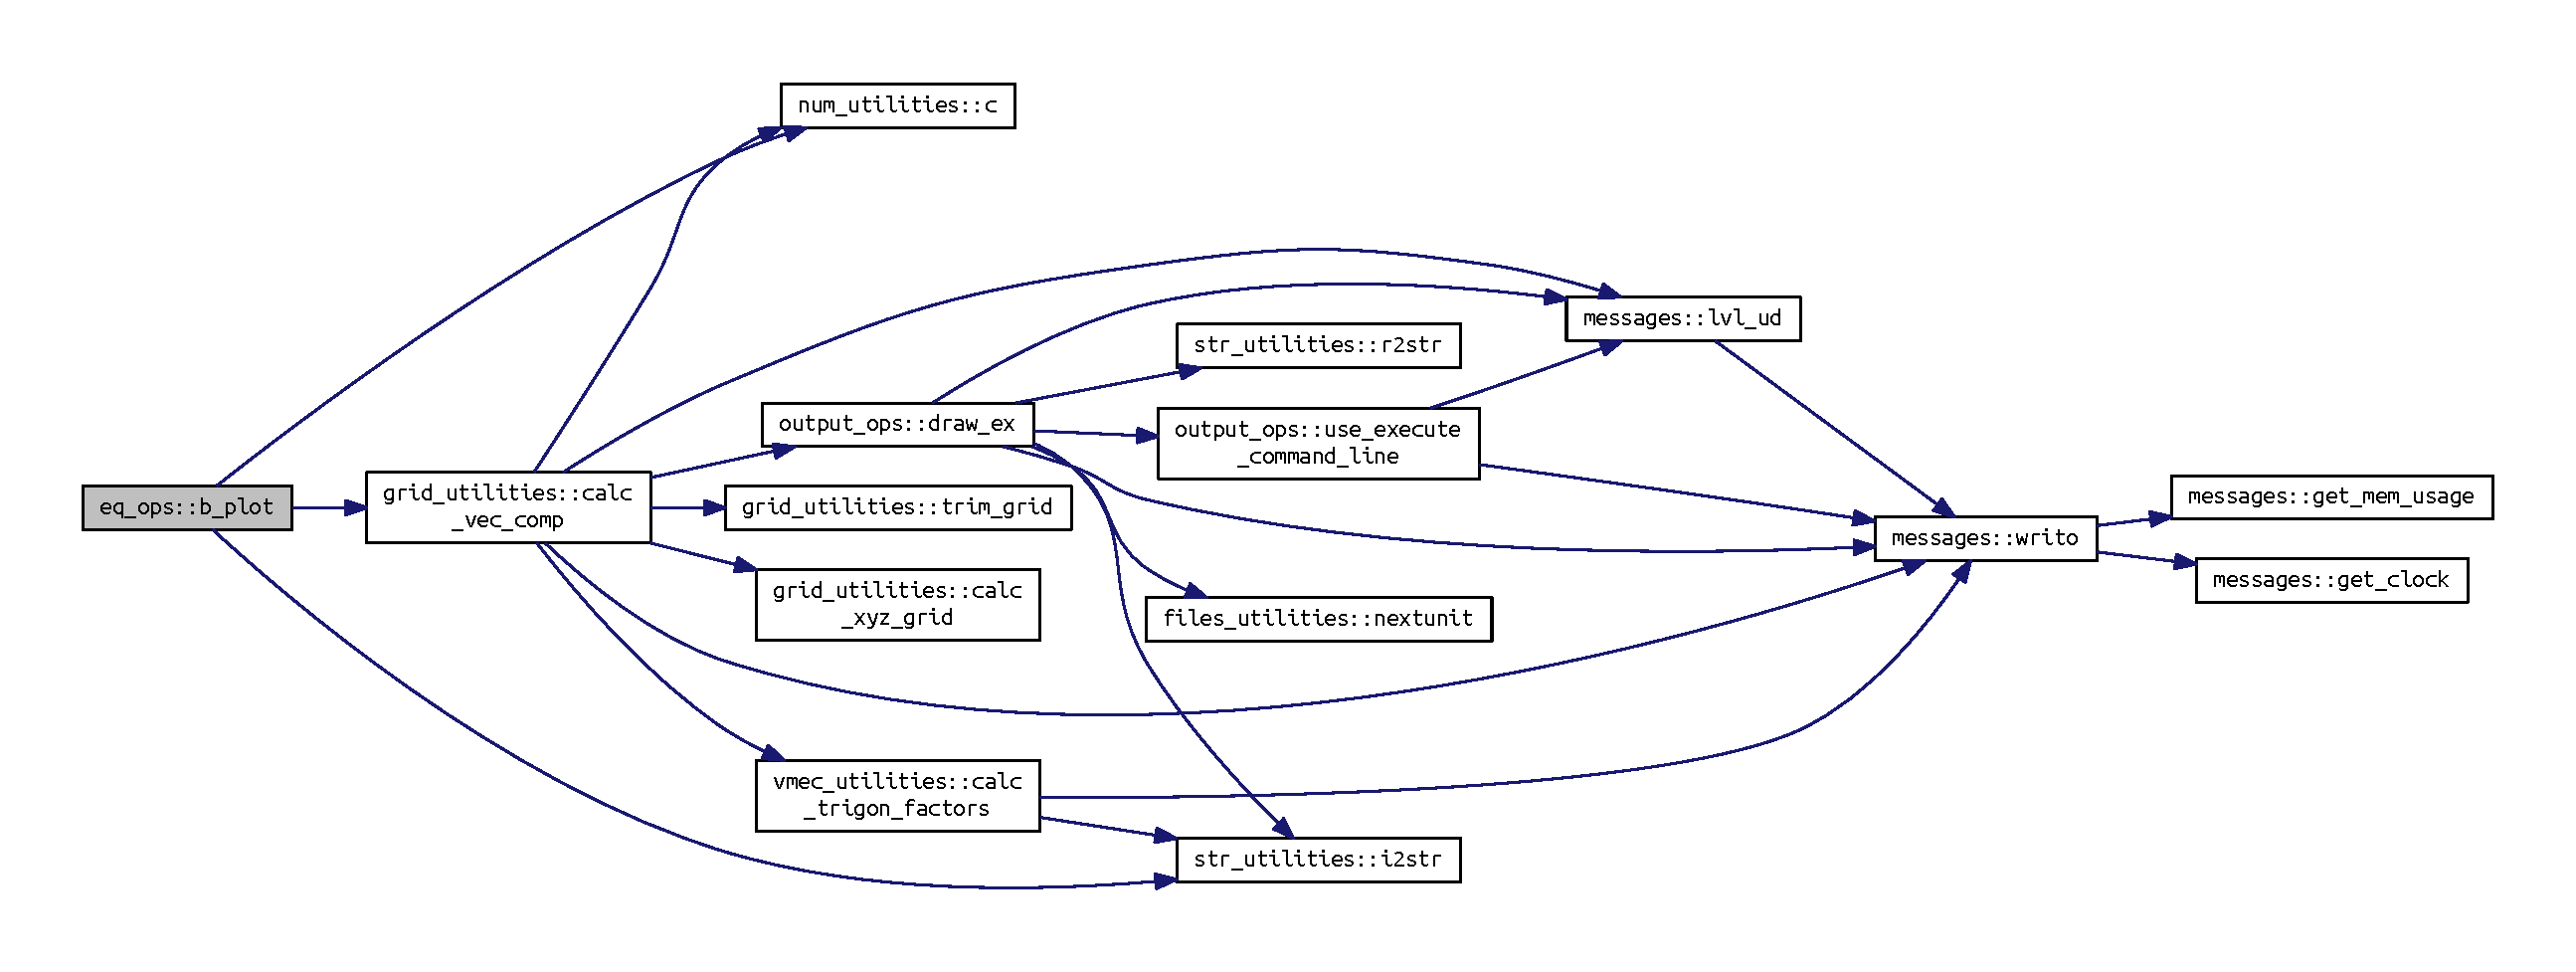
\includegraphics[width=350pt]{namespaceeq__ops_a73a8c3cea1e8a636b4978bc626e0fab0_cgraph}
\end{center}
\end{figure}
Here is the caller graph for this function\+:\nopagebreak
\begin{figure}[H]
\begin{center}
\leavevmode
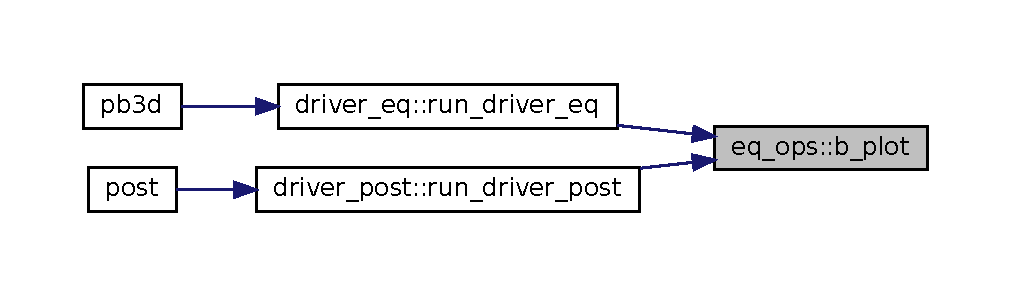
\includegraphics[width=350pt]{namespaceeq__ops_a73a8c3cea1e8a636b4978bc626e0fab0_icgraph}
\end{center}
\end{figure}
\mbox{\Hypertarget{namespaceeq__ops_a087e08ce6d8ad381b5bac8fc51148d50}\label{namespaceeq__ops_a087e08ce6d8ad381b5bac8fc51148d50}} 
\index{eq\+\_\+ops@{eq\+\_\+ops}!calc\+\_\+derived\+\_\+q@{calc\+\_\+derived\+\_\+q}}
\index{calc\+\_\+derived\+\_\+q@{calc\+\_\+derived\+\_\+q}!eq\+\_\+ops@{eq\+\_\+ops}}
\subsubsection{\texorpdfstring{calc\+\_\+derived\+\_\+q()}{calc\_derived\_q()}}
{\footnotesize\ttfamily integer function, public eq\+\_\+ops\+::calc\+\_\+derived\+\_\+q (\begin{DoxyParamCaption}\item[{type(\hyperlink{structgrid__vars_1_1grid__type}{grid\+\_\+type}), intent(in)}]{grid\+\_\+eq,  }\item[{type(\hyperlink{structeq__vars_1_1eq__1__type}{eq\+\_\+1\+\_\+type}), intent(in)}]{eq\+\_\+1,  }\item[{type(\hyperlink{structeq__vars_1_1eq__2__type}{eq\+\_\+2\+\_\+type}), intent(inout), target}]{eq\+\_\+2 }\end{DoxyParamCaption})}



Calculates derived equilibrium quantities system. 


\begin{DoxyItemize}
\item magnetic shear {\ttfamily S} 
\item normal curvature {\ttfamily kappa\+\_\+n} 
\item geodesic curvature {\ttfamily kappa\+\_\+g} 
\item parallel current {\ttfamily sigma} 
\end{DoxyItemize}

Naive implementations of these quantities, with the exception of {\ttfamily S}, give numerically very unfavorable results, so special care must be taken in this procedure.

This is an important issue as these derived equilbrium quantities are important building blocks of the perturbed potential energy, including the drivers of instabilities.

\subsubsection*{The shear }

The local shear $S$ is calculated using equation 3.\+22 from \cite{Weyens3D} \+:

$S = - \frac{1}{\mathcal{J}} \frac{\partial}{\partial \theta} \left(\frac{ h^{\psi\alpha}}{ h^{\psi \psi}}\right)$

which doesn\textquotesingle{}t pose any particular problems as there are only angular derivatives.

\subsubsection*{The curvature }

This is calculated using the parallel derivative of the parallel unit vector (i.\+e. theta if using poloidal flux and zeta if using toroidal flux).

By taking instead the derivative of the covariant basis vector and realizing that the difference with the real curvature lies solely in a component along the parallel direction, which cancels out when taking the normal or geodesic components, the situation becomes easier.

Asuming the poloidal flux is used as normal coordinate, the taks is therefore how to calculate $\frac{1}{\left|\vec{e}_\theta\right|^2} \frac{\partial}{\partial \theta} \vec{e}_\theta$.

By transforming both the derivative as well as the basis vector to Equilibrium coordinates, this can be written as

$\sum_{i=2,3} \sum_{j=2,3} \mathcal{T}_\text{F}^\text{E} \left(3,i\right)) \frac{\partial}{\partial u^i_\text{E}} \left( \mathcal{T}_\text{F}^\text{E} \left(3,j\right) \vec{e}_{j,\text{E}}\right)$

where the summations only run over the angular coordinates because $\vec{e}_\theta$ never has any component along $\vec{e}_{\psi,\text{E}}$.

This double summation formula can then be written as a matrix equation

$\begin{pmatrix}\mathcal{T}_\text{F}^\text{E}\left(3,2\right) & \mathcal{T}_\text{F}^\text{E}\left(3,3\right)\end{pmatrix} \left[ \begin{pmatrix} \frac{\partial}{\partial u^2} \vec{e}_{2} & \frac{\partial}{\partial u^2} \vec{e}_{3} \\ \frac{\partial}{\partial u^3} \vec{e}_{2} & \frac{\partial}{\partial u^3} \vec{e}_{3}\end{pmatrix}_\text{E} \begin{pmatrix}\mathcal{T}_\text{F}^\text{E}\left(3,2\right) \\ \mathcal{T}_\text{F}^\text{E}\left(3,3\right)\end{pmatrix} + \begin{pmatrix} \frac{\partial}{\partial u^2} \mathcal{T}_\text{F}^\text{E}\left(3,2\right) & \frac{\partial}{\partial u^2} \mathcal{T}_\text{F}^\text{E}\left(3,3\right) \\ \frac{\partial}{\partial u^3} \mathcal{T}_\text{F}^\text{E}\left(3,2\right) & \frac{\partial}{\partial u^3} \mathcal{T}_\text{F}^\text{E}\left(3,3\right) \end{pmatrix} \begin{pmatrix}\vec{e}_2 \\ \vec{e}_3\end{pmatrix} \right]$

which can be represented shorthand as $\mathcal{T}_\text{F}^\text{E}\left(3,2:3\right) \left[ \mathcal{D}\vec{e}_\text{E} \mathcal{T}_\text{F}^\text{E}\left(3,2:3\right)^T +\mathcal{D} \mathcal{T} \vec{e}_\text{E}^T \right]$

It is relatively easy to set up the matrix $\mathcal{D}\vec{e}_\text{E}$ as a function of covariant basis vectors in the Cylindrical coordinate system. The derivatives of the transformation matrix itself can likewise be found.

The steps used in this routine are therefore
\begin{DoxyEnumerate}
\item Set up $\mathcal{D}\vec{e}_\text{E}$, i.\+e. as a function of the three cylindrical covariant basis vectors.
\item Set up correctcion by the derivatives of the transformation matrix, with a single summation.
\item Decompose the normal $\frac{\nabla \psi}{\left|\nabla\psi\right|^2}$ and geodesic vectors $\frac{\nabla \psi \times \vec{B}}{B^2}$ as a function of the cylindrical contravariant basis vectors.
\item Double summation to reduce term $\sim$ $\mathcal{D}\vec{e}_\text{E}$ and correction by single summation to reduce term $\sim$ $\mathcal{D}\mathcal{T}$.
\item Dot these for each of the four (actually three because of symmetry) elements of $\mathcal{D}\vec{e}_\text{E}$.
\item Divide by $\left|\vec{e}_\theta\right|^2$.
\item Possibly correct for toroidal flux.
\end{DoxyEnumerate}

An advantage of using this formulation is that no normal derivatives are needed, so that nothing has to implicitely cancel out.

\subsubsection*{The parallel current }

The parallel current is calculated from the shear with the help of equation 3.\+29 of \cite{Weyens3D} \+:

$\mu_0 \sigma = -\frac{1}{B_\theta} \left[ 2 \frac{\nabla \psi \times \vec{B}}{\left|\nabla \psi\right|^2} \cdot \frac{\partial \left(\nabla \psi\right)}{\partial \theta} + \mathcal{J} \left|\nabla \psi\right|^2 S \right]$ .

where a similar technique can be used as above, for the calculation of the curvature\+: As

$\frac{\nabla \psi \times \vec{B}}{\left|\nabla \psi\right|^2} = \frac{B_\theta \vec{e}_\alpha - B_\alpha \vec{e}_\theta} {\mathcal{J} \left|\nabla\psi\right|^2}$ ,

The parallel derivative of $\nabla \psi$ can be rewritten in terms of contravariant components of derivatives of covariant basis vectors\+:

$\left\{ \begin{aligned} \vec{e}_\alpha \cdot \frac{\partial \left(\nabla \psi\right)}{\partial\theta} = - \nabla \psi \cdot \frac{\partial \vec{e}_\theta}{\partial \alpha} \\ \vec{e}_\theta \cdot \frac{\partial \left(\nabla \psi\right)}{\partial\theta} = - \nabla \psi \cdot \frac{\partial \vec{e}_\theta}{\partial \theta} \\ \end{aligned}\right. $ ,

so that the result is\+:

$\frac{\nabla \psi \times \vec{B}}{\left|\nabla \psi\right|^2} \cdot \frac{\partial \left(\nabla \psi\right)}{\partial \theta} = \frac{1}{\mathcal{J}^2} \frac{\nabla \psi}{\left|\nabla\psi\right|^2} \cdot \left[ g_{\alpha\theta} \frac{\partial \vec{e}_\theta}{\partial \theta} - g_{\theta\theta} \frac{\partial \vec{e}_\theta}{\partial \alpha} \right] $ ,

which is given by a formula similar to the one used above for the geodesical curvature.

In debug mode, it can be checked whether the current is indeed divergence-\/free, with the help of equation 3.\+33 of \cite{Weyens3D}.

$ -2 p' \int_{\theta_0}^\theta \mathcal{J} \kappa_g \text{d}{\theta} = \sigma\left(\theta\right) - \sigma_0$

and whether a direct, naive implementation of the parallel current from equation 3.\+26 of \cite{Weyens3D} agrees with the more accurate results used here\+:

$\sigma = \frac{\partial B_\psi}{\partial \alpha} - \frac{\partial B_\alpha}{\partial \psi} - \mu_0 p' \mathcal{J} \frac{B_\alpha}{B_\theta}$ .

The reason why they are generally different is that this implementation relies on the cancellation of large terms.

\begin{DoxyNote}{Note}

\begin{DoxyEnumerate}
\item If the toroidal flux is used instead, the actual curvature obviously is unchanged, which implies that the normal component has to be multiplied by the safety factor and the geodesic component has to be divided by it.
\item The formulas for the normal and geodesic basis vectors for V\+M\+EC are
\begin{DoxyItemize}
\item $\frac{\nabla \psi}{\left|\nabla\psi\right|^2} = -\frac{\mathcal{J} \left(1 + \lambda_\theta\right)} {Z_\theta^2 + R_\theta^2 + \left(R_\zeta Z_\theta - R_\theta Z_\zeta \right)/R^2} \frac{1}{R} \left( -Z_\theta , R_\zeta Z_\theta - R_\theta Z_\zeta, R_\theta\right)_\text{C}$
\item $\frac{\nabla \psi \times \vec{B}}{B^2} = \frac{1}{g_{\theta\theta}} \left(P R_\theta - Q R_\zeta, -Q R^2, P Z_\theta - Q Z_\zeta\right)_\text{C}$
\item $Q = g_{\theta\theta} - q g_{\theta\alpha}$ (using right-\/handed flux $q_\text{F}$, which is the inverse of the left-\/handed V\+M\+EC $q_\text{V}$)
\item $P = \frac{Q \lambda_\zeta - g_{\alpha\theta}}{1+\lambda_\theta}$ (where the derivatives of $R$, $Z$ and $\lambda$ are in V\+M\+EC coordinates).
\end{DoxyItemize}
\item The formulas for the normal and geodesic basis vectors for H\+E\+L\+E\+NA are
\begin{DoxyItemize}
\item $\frac{\nabla \psi}{\left|\nabla\psi\right|^2} = -\frac{1}{Z_\theta^2 + R_\theta^2} \frac{q R}{F} \left( -Z_\theta , 0, R_\theta\right)_\text{C}$
\item $\frac{\nabla \psi \times \vec{B}}{B^2} = \frac{q R^2}{R_\theta^2 + Z_\theta^2 + q^2 R^2} \left(-R_\theta, -\frac{R_\theta^2 + Z_\theta^2}{q}, -Z_\theta\right)_\text{C}$
\end{DoxyItemize}
\item The expression for $\mathcal{J}\left|\nabla \psi\right|^2 S + \mu_0 \mathcal{J}B^2 \sigma$ for H\+E\+L\+E\+NA is $- 2 \frac{F}{R} \left( \frac{Z_\theta}{R} + \frac{Z_\theta R_{\theta\theta} - R_\theta Z_{\theta\theta}}{R_\theta^2 + Z_\theta^2} \right)$.
\end{DoxyEnumerate}
\end{DoxyNote}

\begin{DoxyParams}[1]{Parameters}
\mbox{\tt in}  & {\em grid\+\_\+eq} & equilibrium grid\\
\hline
\mbox{\tt in}  & {\em eq\+\_\+1} & flux equilibrium variables\\
\hline
\mbox{\tt in,out}  & {\em eq\+\_\+2} & metric equilibrium variables \\
\hline
\end{DoxyParams}


Definition at line 4186 of file eq\+\_\+ops.\+f90.

Here is the call graph for this function\+:\nopagebreak
\begin{figure}[H]
\begin{center}
\leavevmode
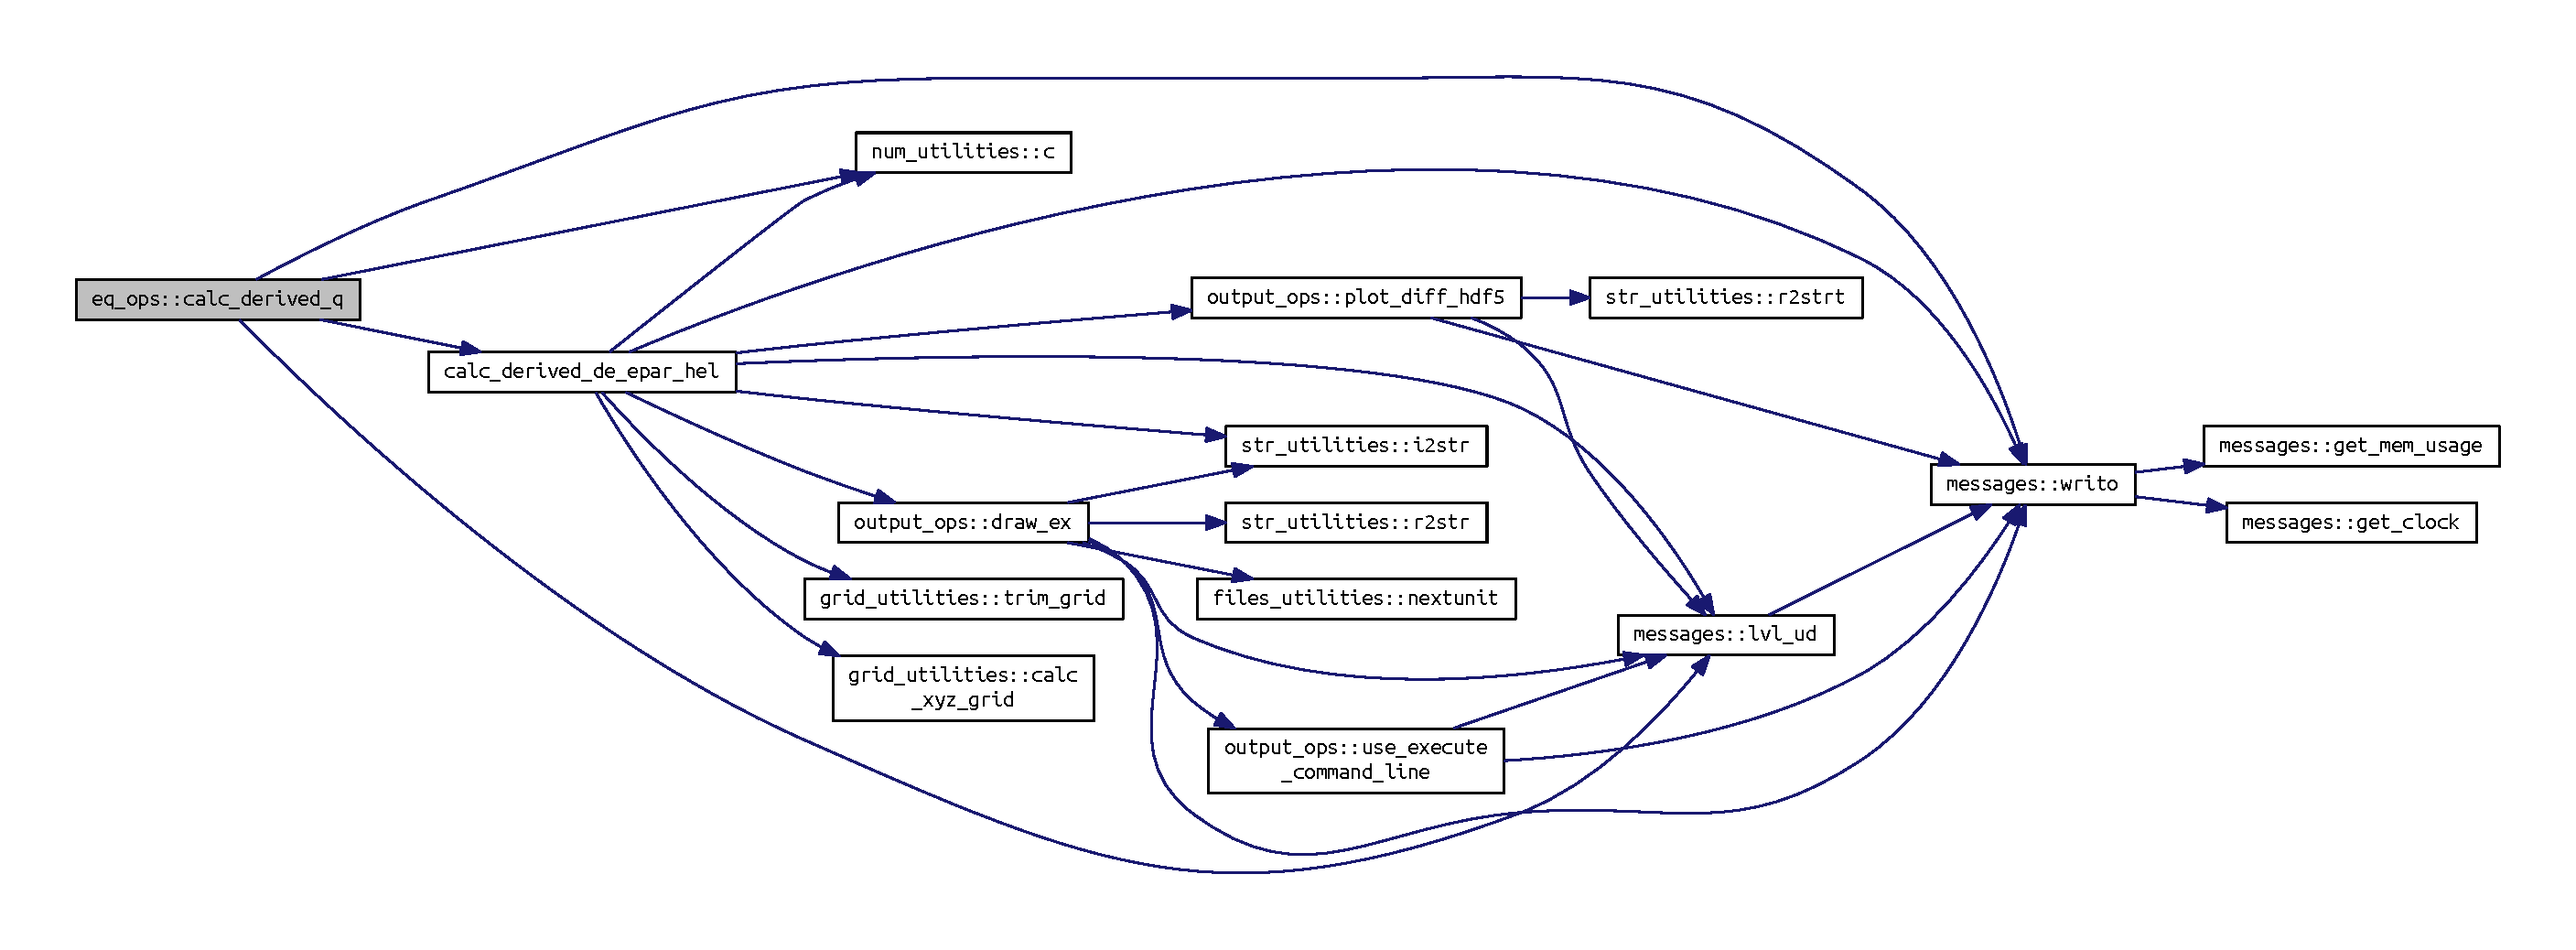
\includegraphics[width=350pt]{namespaceeq__ops_a087e08ce6d8ad381b5bac8fc51148d50_cgraph}
\end{center}
\end{figure}
Here is the caller graph for this function\+:\nopagebreak
\begin{figure}[H]
\begin{center}
\leavevmode
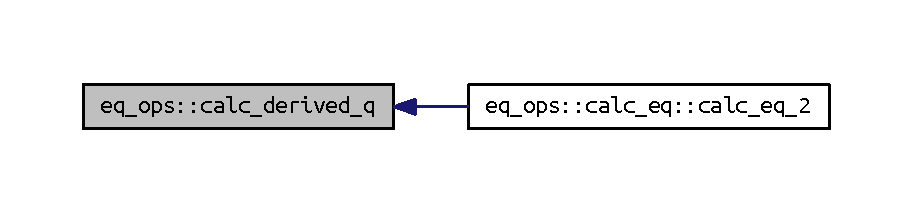
\includegraphics[width=350pt]{namespaceeq__ops_a087e08ce6d8ad381b5bac8fc51148d50_icgraph}
\end{center}
\end{figure}
\mbox{\Hypertarget{namespaceeq__ops_a4e20b8725fce149449f83754244dc84e}\label{namespaceeq__ops_a4e20b8725fce149449f83754244dc84e}} 
\index{eq\+\_\+ops@{eq\+\_\+ops}!calc\+\_\+eq\+\_\+jobs\+\_\+lims@{calc\+\_\+eq\+\_\+jobs\+\_\+lims}}
\index{calc\+\_\+eq\+\_\+jobs\+\_\+lims@{calc\+\_\+eq\+\_\+jobs\+\_\+lims}!eq\+\_\+ops@{eq\+\_\+ops}}
\subsubsection{\texorpdfstring{calc\+\_\+eq\+\_\+jobs\+\_\+lims()}{calc\_eq\_jobs\_lims()}}
{\footnotesize\ttfamily integer function, public eq\+\_\+ops\+::calc\+\_\+eq\+\_\+jobs\+\_\+lims (\begin{DoxyParamCaption}\item[{integer, intent(in)}]{n\+\_\+par\+\_\+X,  }\item[{integer, intent(in)}]{n\+\_\+div }\end{DoxyParamCaption})}



Calculate {\ttfamily eq\+\_\+jobs\+\_\+lims}. 

Take into account that every job has to start and end at the start and end of a fundamental integration interval, as discussed in \hyperlink{namespaceeq__ops_a8fae749abe55865d8135fef536a8e8f1}{divide\+\_\+eq\+\_\+jobs()}\+:
\begin{DoxyItemize}
\item for {\ttfamily magn\+\_\+int\+\_\+style=1} (trapezoidal), this is 1 point,
\item for {\ttfamily magn\+\_\+int\+\_\+style=2} (Simpson 3/8), this is 3 points.
\end{DoxyItemize}

for P\+O\+ST, there are no Richardson levels, and there has to be overlap of one always, in order to have correct composite integrals of the different regions.

\begin{DoxyNote}{Note}
The {\ttfamily n\+\_\+par\+\_\+X} passed into this procedure refers to the quantity that is already possibly halved if the Richardson level is higher than 1. This information is then reflected in the eq\+\_\+jobs\+\_\+lims, which refer to the local limits, i.\+e. only the parallel points currently under consideration.
\end{DoxyNote}
\begin{DoxyReturn}{Returns}
ierr
\end{DoxyReturn}

\begin{DoxyParams}[1]{Parameters}
\mbox{\tt in}  & {\em n\+\_\+par\+\_\+x} & number of parallel points in this Richardson level\\
\hline
\mbox{\tt in}  & {\em n\+\_\+div} & nr. of divisions of parallel ranges \\
\hline
\end{DoxyParams}


Definition at line 6055 of file eq\+\_\+ops.\+f90.

Here is the caller graph for this function\+:\nopagebreak
\begin{figure}[H]
\begin{center}
\leavevmode
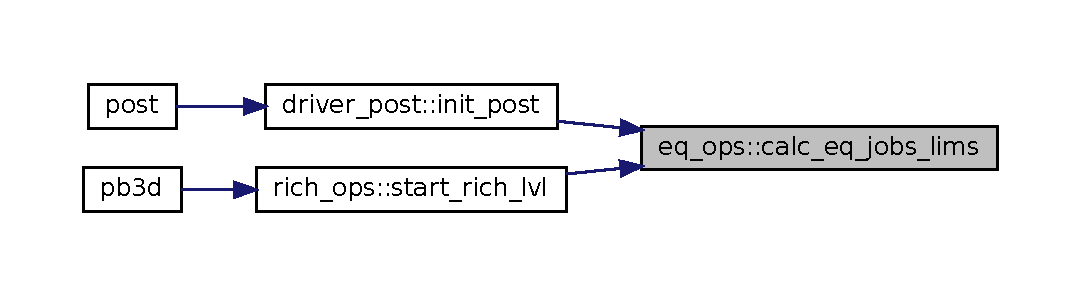
\includegraphics[width=350pt]{namespaceeq__ops_a4e20b8725fce149449f83754244dc84e_icgraph}
\end{center}
\end{figure}
\mbox{\Hypertarget{namespaceeq__ops_a7cd38586e386e1bc684a327ebcc4c1de}\label{namespaceeq__ops_a7cd38586e386e1bc684a327ebcc4c1de}} 
\index{eq\+\_\+ops@{eq\+\_\+ops}!calc\+\_\+normalization\+\_\+const@{calc\+\_\+normalization\+\_\+const}}
\index{calc\+\_\+normalization\+\_\+const@{calc\+\_\+normalization\+\_\+const}!eq\+\_\+ops@{eq\+\_\+ops}}
\subsubsection{\texorpdfstring{calc\+\_\+normalization\+\_\+const()}{calc\_normalization\_const()}}
{\footnotesize\ttfamily integer function, public eq\+\_\+ops\+::calc\+\_\+normalization\+\_\+const (\begin{DoxyParamCaption}{ }\end{DoxyParamCaption})}



Sets up normalization constants. 


\begin{DoxyItemize}
\item V\+M\+EC version ({\ttfamily eq\+\_\+style=1})\+:~\newline
 Normalization depends on {\ttfamily norm\+\_\+style\+:} 
\begin{DoxyEnumerate}
\item M\+I\+S\+H\+KA
\begin{DoxyItemize}
\item R\+\_\+0\+: major radius (= average magnetic axis)
\item B\+\_\+0\+: B on magnetic axis (theta = zeta = 0)
\item pres\+\_\+0\+: reference pressure (= B\+\_\+0$^\wedge$2/mu\+\_\+0)
\item psi\+\_\+0\+: reference flux (= R\+\_\+0$^\wedge$2 B\+\_\+0)
\item rho\+\_\+0\+: reference mass density
\end{DoxyItemize}
\item C\+O\+B\+RA
\begin{DoxyItemize}
\item R\+\_\+0\+: major radius (= average geometric axis)
\item pres\+\_\+0\+: pressure on magnetic axis
\item B\+\_\+0\+: reference magnetic field (= sqrt(2pres\+\_\+0mu\+\_\+0 / beta))
\item psi\+\_\+0\+: reference flux (= R\+\_\+0$^\wedge$2 B\+\_\+0 / aspr$^\wedge$2)
\item rho\+\_\+0\+: reference mass density where aspr (aspect ratio) and beta are given by V\+M\+EC.
\end{DoxyItemize}
\end{DoxyEnumerate}
\item H\+E\+L\+E\+NA version ({\ttfamily eq\+\_\+style=2})\+:~\newline
 Normalization is used by default and does not depend on {\ttfamily norm\+\_\+style} 
\end{DoxyItemize}

\begin{DoxySeeAlso}{See also}
\hyperlink{namespacehelena__ops_ae05ba1182eb002d93c27ca4ff7ab8cf2}{read\+\_\+hel()}
\end{DoxySeeAlso}
\begin{DoxyNote}{Note}
{\ttfamily rho\+\_\+0} is not given through by the equilibrium codes and should be user-\/supplied
\end{DoxyNote}
\begin{DoxyReturn}{Returns}
ierr 
\end{DoxyReturn}


Definition at line 4759 of file eq\+\_\+ops.\+f90.

Here is the call graph for this function\+:\nopagebreak
\begin{figure}[H]
\begin{center}
\leavevmode
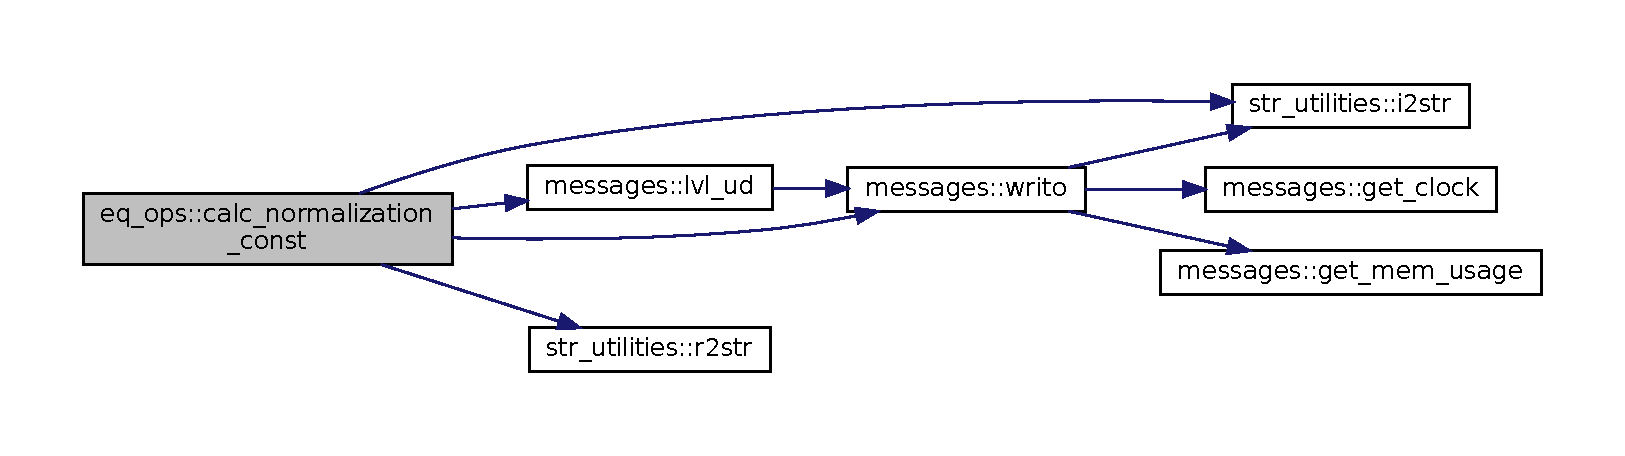
\includegraphics[width=350pt]{namespaceeq__ops_a7cd38586e386e1bc684a327ebcc4c1de_cgraph}
\end{center}
\end{figure}
Here is the caller graph for this function\+:\nopagebreak
\begin{figure}[H]
\begin{center}
\leavevmode
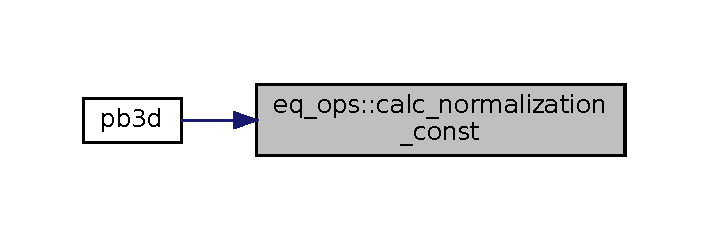
\includegraphics[width=330pt]{namespaceeq__ops_a7cd38586e386e1bc684a327ebcc4c1de_icgraph}
\end{center}
\end{figure}
\mbox{\Hypertarget{namespaceeq__ops_a9addef683b3d4a8c587510e4c994ec61}\label{namespaceeq__ops_a9addef683b3d4a8c587510e4c994ec61}} 
\index{eq\+\_\+ops@{eq\+\_\+ops}!create\+\_\+vmec\+\_\+input@{create\+\_\+vmec\+\_\+input}}
\index{create\+\_\+vmec\+\_\+input@{create\+\_\+vmec\+\_\+input}!eq\+\_\+ops@{eq\+\_\+ops}}
\subsubsection{\texorpdfstring{create\+\_\+vmec\+\_\+input()}{create\_vmec\_input()}}
{\footnotesize\ttfamily integer function eq\+\_\+ops\+::create\+\_\+vmec\+\_\+input (\begin{DoxyParamCaption}\item[{type(\hyperlink{structgrid__vars_1_1grid__type}{grid\+\_\+type}), intent(in)}]{grid\+\_\+eq,  }\item[{type(\hyperlink{structeq__vars_1_1eq__1__type}{eq\+\_\+1\+\_\+type}), intent(in)}]{eq\+\_\+1 }\end{DoxyParamCaption})}



Creates a V\+M\+EC input file. 

Optionally, a perturbation can be added\+: Either the displacement of the plasma position can be described ({\ttfamily pert\+\_\+style} 1), or ripple in the toroidal magnetic field ({\ttfamily pert\+\_\+style} 2), with a fixed toroidal mode number.

Both perturbation styles can have various prescription types\+:
\begin{DoxyEnumerate}
\item file with Fourier modes in the geometrical angular coordinate
\item same but manually
\item file with perturbation from a 2-\/D map in the geometric angular coordinate.
\end{DoxyEnumerate}

For {\ttfamily pert\+\_\+style} 2, a file has to be provided that describes the translation between position perturbation and magnetic perturbation for curves of constant geometrical angle. This file can be generated for an already existing ripple case using P\+O\+ST with {\ttfamily --compare\+\_\+tor\+\_\+pos} with {\ttfamily n\+\_\+zeta\+\_\+plot = 3} and {\ttfamily min\+\_\+theta\+\_\+plot} and {\ttfamily max\+\_\+theta\+\_\+plot} indicating half a ripple period.

The output from this V\+M\+EC run can then be used to iteratively create a new file to translate toroidal magnetic field ripple to position perturbation.

\begin{DoxyNote}{Note}
Meaning of the indices of {\ttfamily B\+\_\+F}, {\ttfamily B\+\_\+\+F\+\_\+dum\+:} 
\begin{DoxyItemize}
\item {\ttfamily (pol modes, cos/sin)} for {\ttfamily B\+\_\+\+F\+\_\+dum} 
\item {\ttfamily (tor\+\_\+modes, pol modes, cos/sin (m theta), R/Z)} for {\ttfamily B\+\_\+F} 
\end{DoxyItemize}
\end{DoxyNote}

\begin{DoxyParams}[1]{Parameters}
\mbox{\tt in}  & {\em grid\+\_\+eq} & equilibrium grid varibles\\
\hline
\mbox{\tt in}  & {\em eq\+\_\+1} & flux equilibrium quantities \\
\hline
\end{DoxyParams}


Definition at line 753 of file eq\+\_\+ops.\+f90.

Here is the call graph for this function\+:\nopagebreak
\begin{figure}[H]
\begin{center}
\leavevmode
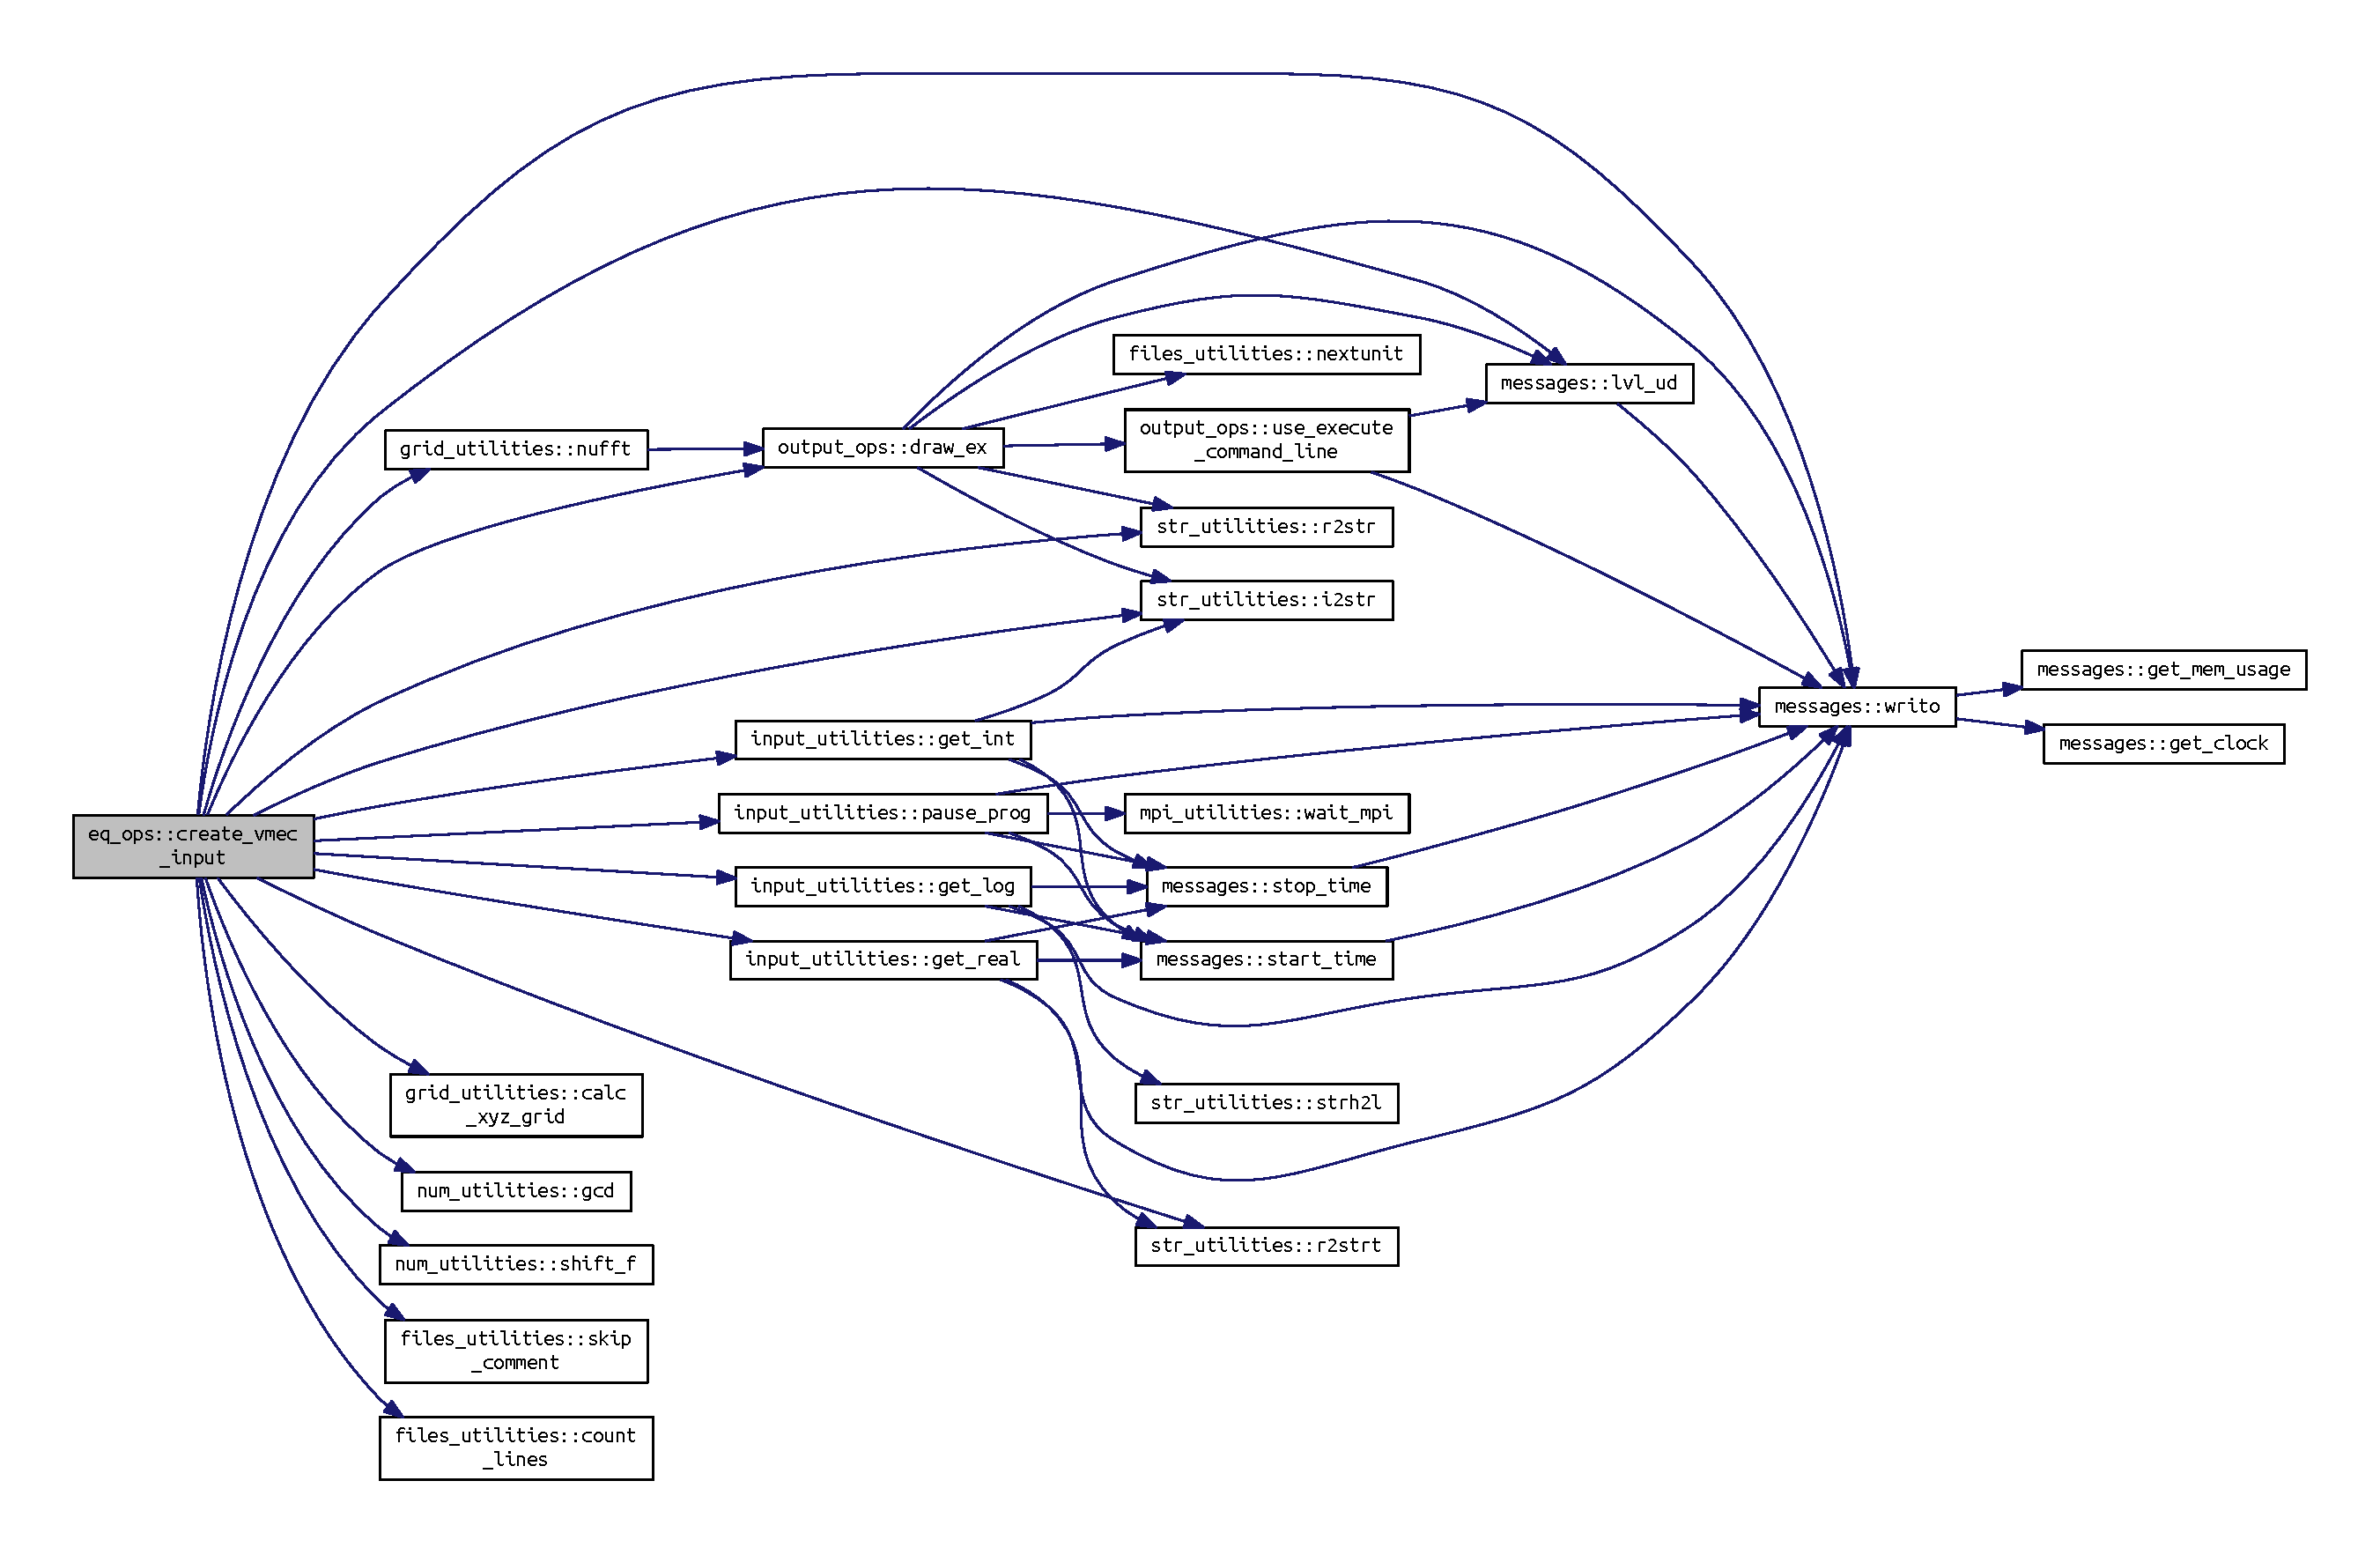
\includegraphics[width=350pt]{namespaceeq__ops_a9addef683b3d4a8c587510e4c994ec61_cgraph}
\end{center}
\end{figure}
Here is the caller graph for this function\+:\nopagebreak
\begin{figure}[H]
\begin{center}
\leavevmode
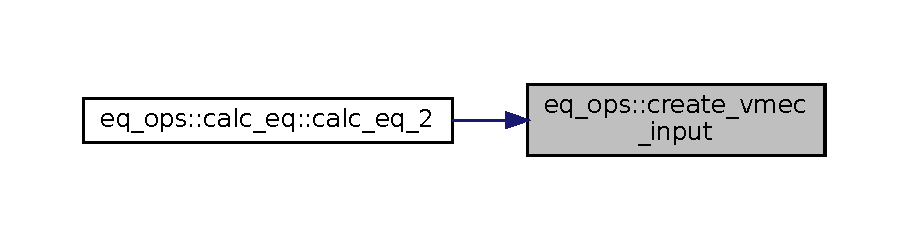
\includegraphics[width=350pt]{namespaceeq__ops_a9addef683b3d4a8c587510e4c994ec61_icgraph}
\end{center}
\end{figure}
\mbox{\Hypertarget{namespaceeq__ops_ac0a79893900631d25b170be0abd2c131}\label{namespaceeq__ops_ac0a79893900631d25b170be0abd2c131}} 
\index{eq\+\_\+ops@{eq\+\_\+ops}!delta\+\_\+r\+\_\+plot@{delta\+\_\+r\+\_\+plot}}
\index{delta\+\_\+r\+\_\+plot@{delta\+\_\+r\+\_\+plot}!eq\+\_\+ops@{eq\+\_\+ops}}
\subsubsection{\texorpdfstring{delta\+\_\+r\+\_\+plot()}{delta\_r\_plot()}}
{\footnotesize\ttfamily integer function, public eq\+\_\+ops\+::delta\+\_\+r\+\_\+plot (\begin{DoxyParamCaption}\item[{type(\hyperlink{structgrid__vars_1_1grid__type}{grid\+\_\+type}), intent(inout)}]{grid\+\_\+eq,  }\item[{type(\hyperlink{structeq__vars_1_1eq__1__type}{eq\+\_\+1\+\_\+type}), intent(in)}]{eq\+\_\+1,  }\item[{type(\hyperlink{structeq__vars_1_1eq__2__type}{eq\+\_\+2\+\_\+type}), intent(in)}]{eq\+\_\+2,  }\item[{real(dp), dimension(\+:,\+:,\+:,\+:), intent(in)}]{X\+YZ,  }\item[{integer, intent(in), optional}]{rich\+\_\+lvl }\end{DoxyParamCaption})}



Plots {\bfseries H\+A\+LF} of the change in the position vectors for 2 different toroidal positions, which can correspond to a ripple. 

Also calculates {\bfseries H\+A\+LF} of the relative magnetic perturbation, which also corresponds to a ripple.

Finally, if the output grid contains a fundamental interval $2\pi$, the proportionality between both is written to a file.

\begin{DoxyNote}{Note}
The metric factors and transformation matrices have to be allocated.
\end{DoxyNote}
\begin{DoxyReturn}{Returns}
ierr
\end{DoxyReturn}

\begin{DoxyParams}[1]{Parameters}
\mbox{\tt in,out}  & {\em grid\+\_\+eq} & equilibrium grid\\
\hline
\mbox{\tt in}  & {\em eq\+\_\+1} & flux equilibrium variables\\
\hline
\mbox{\tt in}  & {\em eq\+\_\+2} & metric equilibrium variables\\
\hline
\mbox{\tt in}  & {\em xyz} & X, Y and Z of grid\\
\hline
\mbox{\tt in}  & {\em rich\+\_\+lvl} & Richardson level \\
\hline
\end{DoxyParams}


Definition at line 5527 of file eq\+\_\+ops.\+f90.

Here is the call graph for this function\+:\nopagebreak
\begin{figure}[H]
\begin{center}
\leavevmode
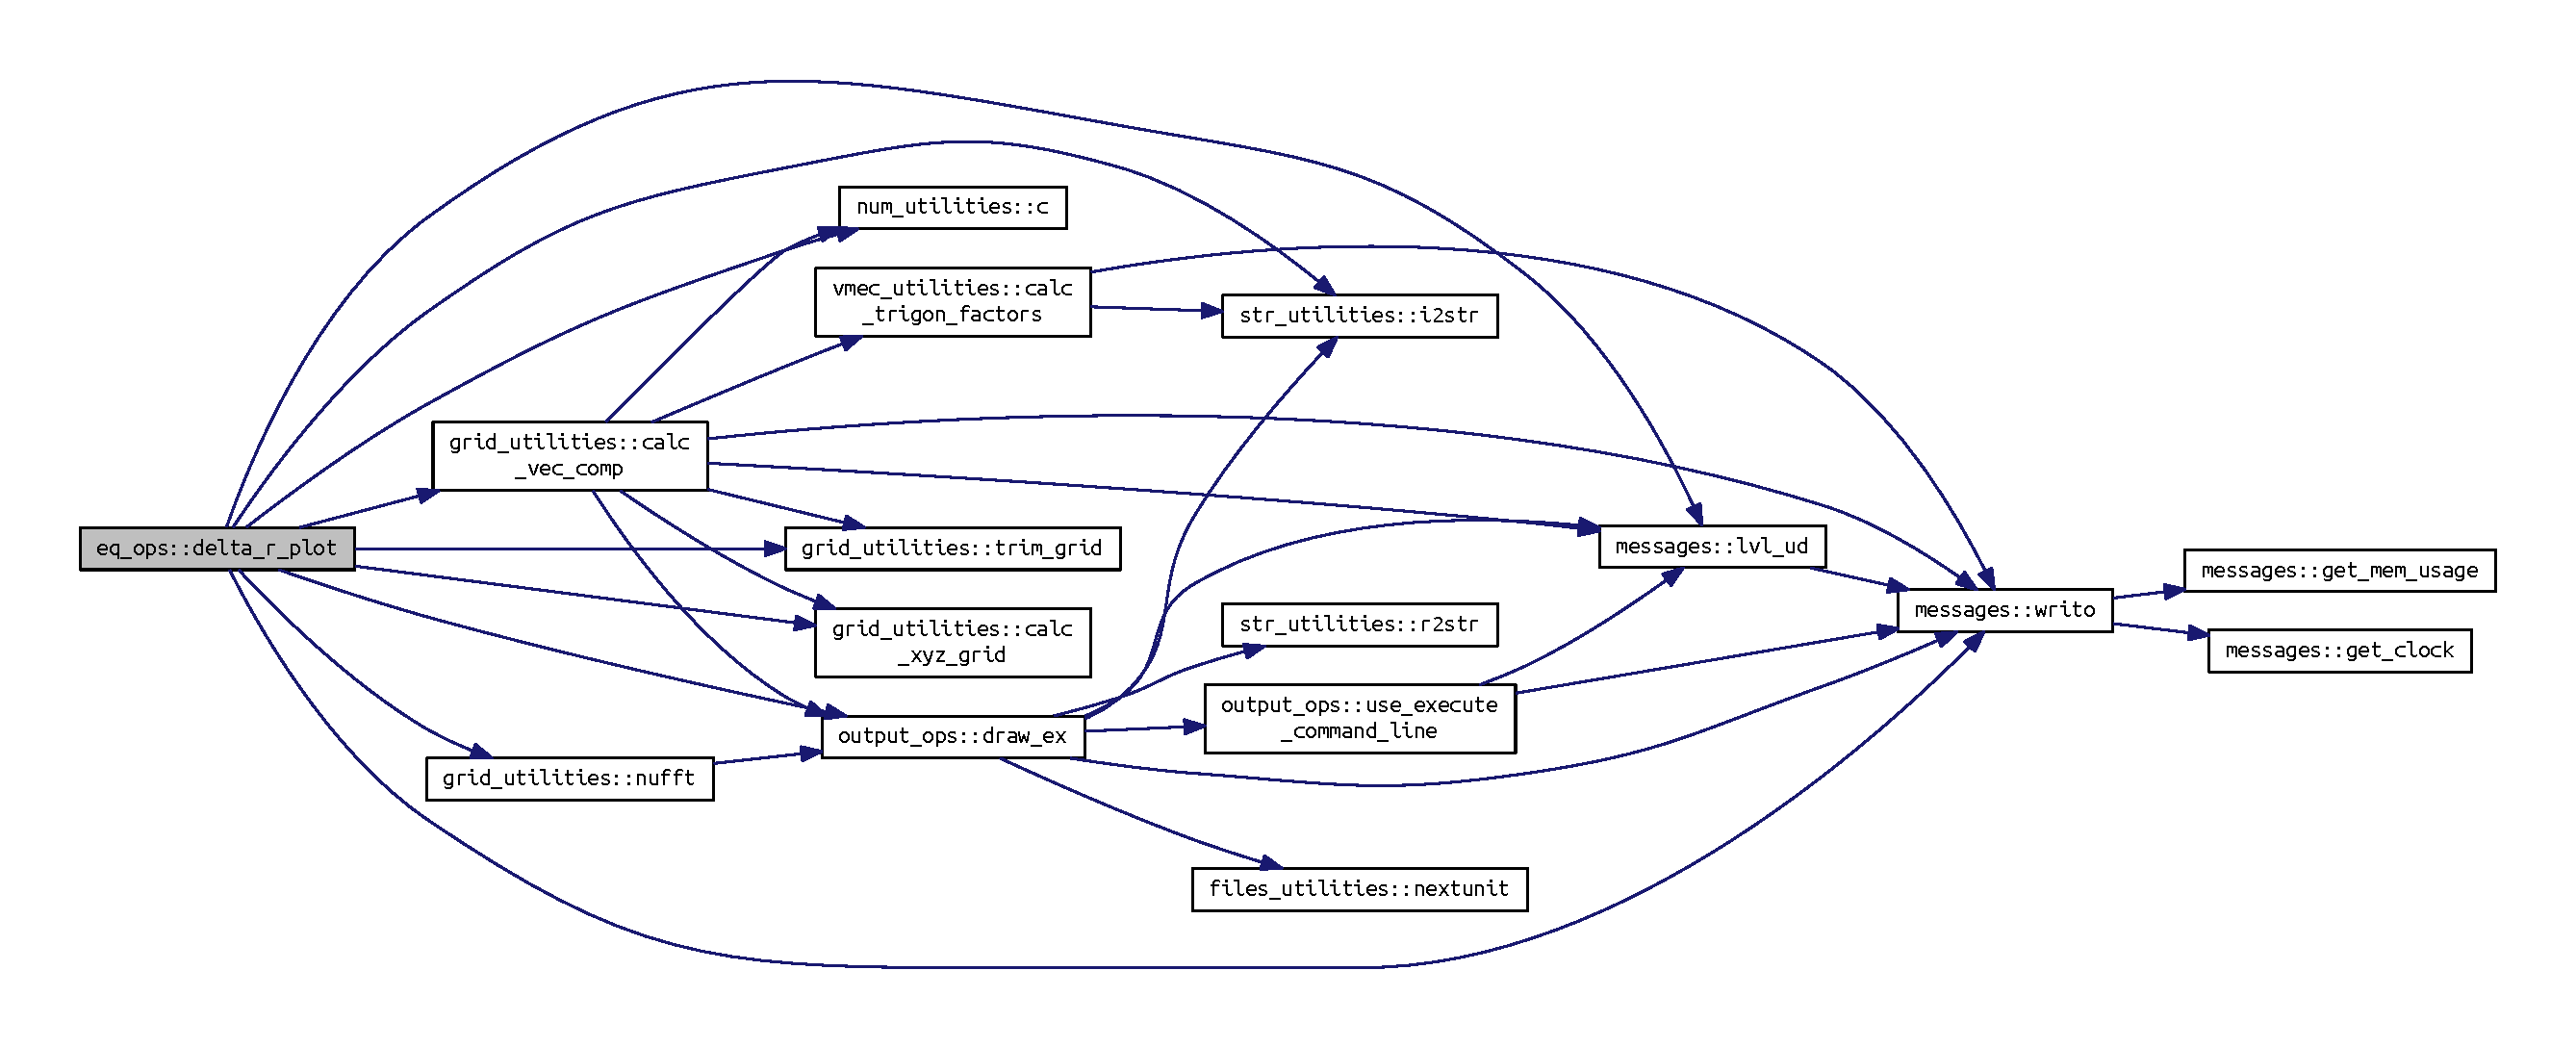
\includegraphics[width=350pt]{namespaceeq__ops_ac0a79893900631d25b170be0abd2c131_cgraph}
\end{center}
\end{figure}
Here is the caller graph for this function\+:\nopagebreak
\begin{figure}[H]
\begin{center}
\leavevmode
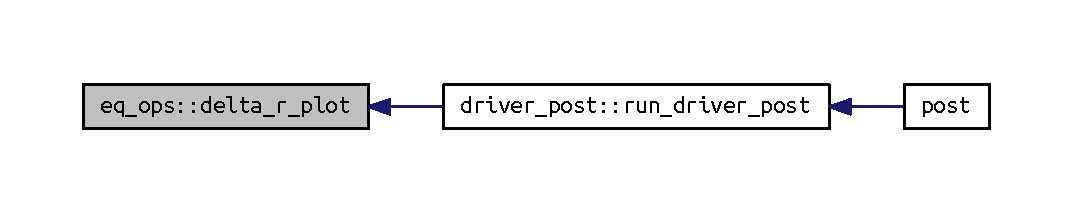
\includegraphics[width=350pt]{namespaceeq__ops_ac0a79893900631d25b170be0abd2c131_icgraph}
\end{center}
\end{figure}
\mbox{\Hypertarget{namespaceeq__ops_a8fae749abe55865d8135fef536a8e8f1}\label{namespaceeq__ops_a8fae749abe55865d8135fef536a8e8f1}} 
\index{eq\+\_\+ops@{eq\+\_\+ops}!divide\+\_\+eq\+\_\+jobs@{divide\+\_\+eq\+\_\+jobs}}
\index{divide\+\_\+eq\+\_\+jobs@{divide\+\_\+eq\+\_\+jobs}!eq\+\_\+ops@{eq\+\_\+ops}}
\subsubsection{\texorpdfstring{divide\+\_\+eq\+\_\+jobs()}{divide\_eq\_jobs()}}
{\footnotesize\ttfamily integer function, public eq\+\_\+ops\+::divide\+\_\+eq\+\_\+jobs (\begin{DoxyParamCaption}\item[{integer, intent(in)}]{n\+\_\+par\+\_\+X,  }\item[{integer, dimension(2), intent(in)}]{arr\+\_\+size,  }\item[{integer, intent(inout)}]{n\+\_\+div,  }\item[{integer, intent(in), optional}]{n\+\_\+div\+\_\+max,  }\item[{integer, intent(in), optional}]{n\+\_\+par\+\_\+\+X\+\_\+base,  }\item[{character(len=$\ast$), intent(in), optional}]{range\+\_\+name }\end{DoxyParamCaption})}



Divides the equilibrium jobs. 

For P\+B3D, the entire parallel range has to be calculated, but due to memory limits this has to be split up in pieces. Every piece has to be able to contain the equilibrium variables (see note below), as well as the vectorial perturbation variables. These are later combined into tensorial variables and integrated.

The equilibrium variables have to be operated on to calculate them, which translates to a scale factor {\ttfamily mem\+\_\+scale\+\_\+fac}. However, in the perturbation phase, when they are just used, this scale factor is not needed.

In its most extreme form, the division in equilibrium jobs would be the individual calculation on a fundamental integration integral of the parallel points\+:
\begin{DoxyItemize}
\item for {\ttfamily magn\+\_\+int\+\_\+style=1} (trapezoidal), this is 1 point,
\item for {\ttfamily magn\+\_\+int\+\_\+style=2} (Simpson 3/8), this is 3 points.
\end{DoxyItemize}

For H\+E\+L\+E\+NA, the parallel derivatives are calculated discretely, the equilibrium and vectorial perturbation variables are tabulated first in this H\+E\+L\+E\+NA grid. This happens in the first Richardson level. In all Richardson levels, afterwards, these variables are interpolated in the angular directions. In this case, therefore, there can be no division of this H\+E\+L\+E\+NA output interval for the first Richardson level.

This procedure does the job of dividing the grids setting the global variables {\ttfamily eq\+\_\+jobs\+\_\+lims}.

The integration of the tensorial perturbation variables is adjusted\+:
\begin{DoxyItemize}
\item If the first job of the parallel jobs and not the first Richardson level\+: add half of the integrated tensorial perturbation quantities of the previous level.
\item If not the first job of the parallel jobs, add the integrated tensorial perturbation quantities to those of the previous parallel job, same Richardson level.
\end{DoxyItemize}

In fact, the equilibrium jobs have much in common with the Richardson levels, as is attested by the existence of the routines \hyperlink{namespaceeq__utilities_a5109472305101af3a15e8e8717c426fd}{do\+\_\+eq()} and \hyperlink{namespaceeq__utilities_a34c5ddab45a54a6c738e5e0b8c7d55d6}{eq\+\_\+info()}, which are equivalent to \hyperlink{namespacerich__ops_a50f4088b9ddd59597987fb4112f2a73e}{do\+\_\+rich()} and \hyperlink{namespacerich__vars_a4f54d3fc0ac510fc073220794ee4fa37}{rich\+\_\+info()}.

In P\+O\+ST, finally, the situation is slightly different for H\+E\+L\+E\+NA, as all the requested variables have to fit, including the interpolated variables, as they are stored whereas in P\+B3D they are not. The parallel range to be taken is then the one of the output grid, including a base range for the variables tabulated on the H\+E\+L\+E\+NA grid. Also, for extended output grids, the size of the grid in the secondary angle has to be included in {\ttfamily n\+\_\+par\+\_\+X} (i.\+e. toroidal when poloidal flux is used and vice versa). Furthermore, multiple equilibrium jobs are allowed.

To this end, optionally, a base number can be provided for {\ttfamily n\+\_\+par\+\_\+X}, that is always added to the number of points in the divided {\ttfamily n\+\_\+par\+\_\+X}.

\begin{DoxyNote}{Note}
For P\+B3D, only the variables {\ttfamily g\+\_\+\+FD}, {\ttfamily h\+\_\+\+FD} and {\ttfamily jac\+\_\+\+FD} are counted, as the equilibrium variables and the transformation matrices are deleted after use. Also, {\ttfamily S}, {\ttfamily sigma}, {\ttfamily kappa\+\_\+n} and {\ttfamily kappa\+\_\+g} can be neglected as they do not contain derivatives and are therefore much smaller. in both routines \hyperlink{namespaceeq__utilities_a5a9f230ed9a6e627e31e882e9f4a00a1}{calc\+\_\+memory\+\_\+eq()} and \hyperlink{namespacex__utilities_a4d18921da77463d069346f1c7322b451}{calc\+\_\+memory\+\_\+x()}, however, a 50\% safety factor is used to account for this somewhat.
\end{DoxyNote}
\begin{DoxyReturn}{Returns}
ierr
\end{DoxyReturn}

\begin{DoxyParams}[1]{Parameters}
\mbox{\tt in}  & {\em n\+\_\+par\+\_\+x} & number of parallel points to be divided\\
\hline
\mbox{\tt in}  & {\em arr\+\_\+size} & array size (using loc\+\_\+n\+\_\+r) for eq\+\_\+2 and X\+\_\+1 variables\\
\hline
\mbox{\tt in,out}  & {\em n\+\_\+div} & final number of divisions\\
\hline
\mbox{\tt in}  & {\em n\+\_\+div\+\_\+max} & maximum n\+\_\+div\\
\hline
\mbox{\tt in}  & {\em n\+\_\+par\+\_\+x\+\_\+base} & base n\+\_\+par\+\_\+X, undivisible\\
\hline
\mbox{\tt in}  & {\em range\+\_\+name} & name of range \\
\hline
\end{DoxyParams}


Definition at line 5920 of file eq\+\_\+ops.\+f90.

Here is the call graph for this function\+:\nopagebreak
\begin{figure}[H]
\begin{center}
\leavevmode
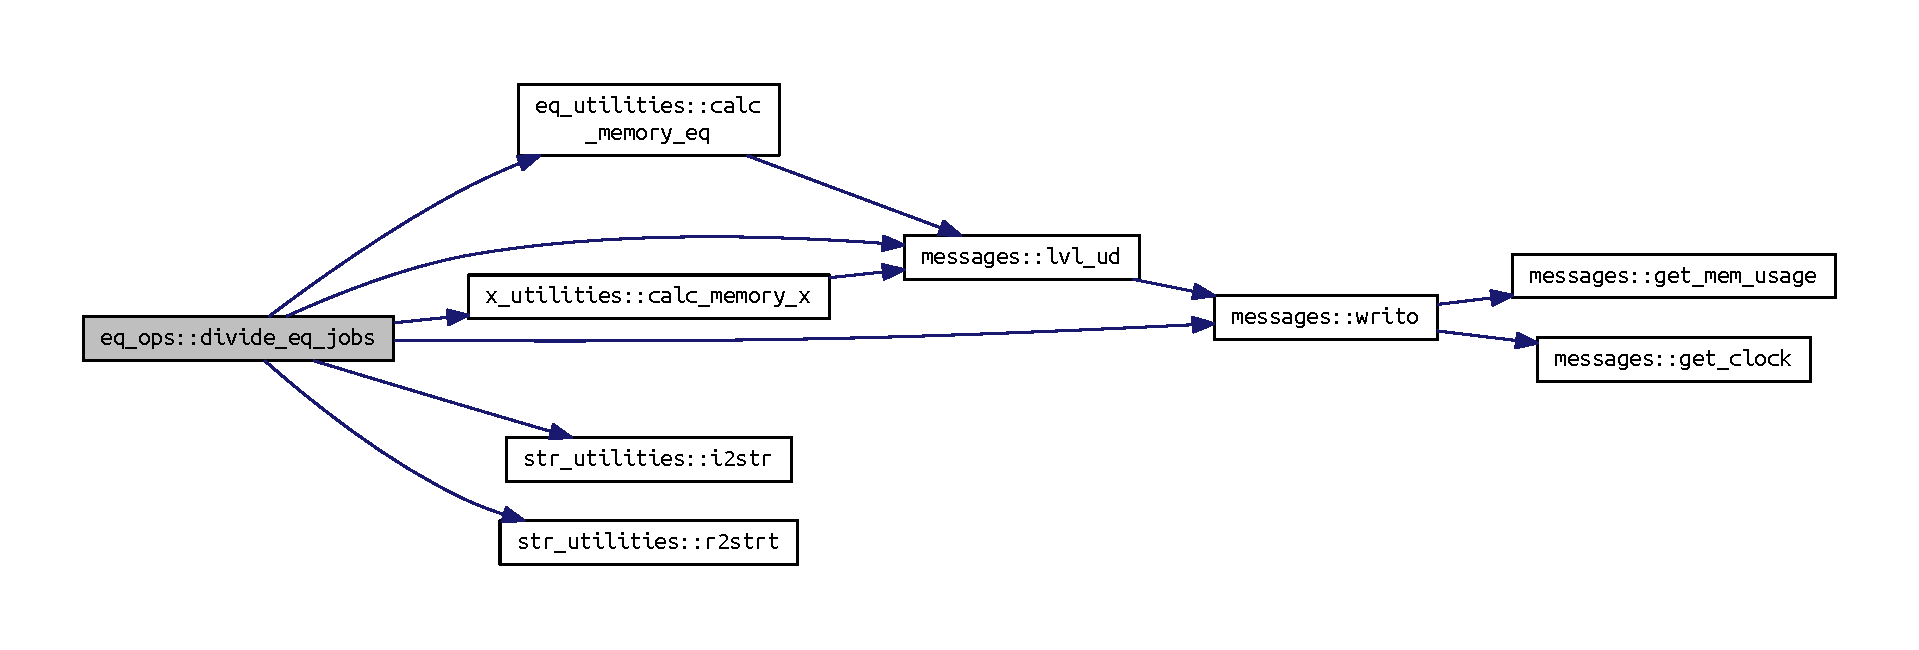
\includegraphics[width=350pt]{namespaceeq__ops_a8fae749abe55865d8135fef536a8e8f1_cgraph}
\end{center}
\end{figure}
Here is the caller graph for this function\+:\nopagebreak
\begin{figure}[H]
\begin{center}
\leavevmode
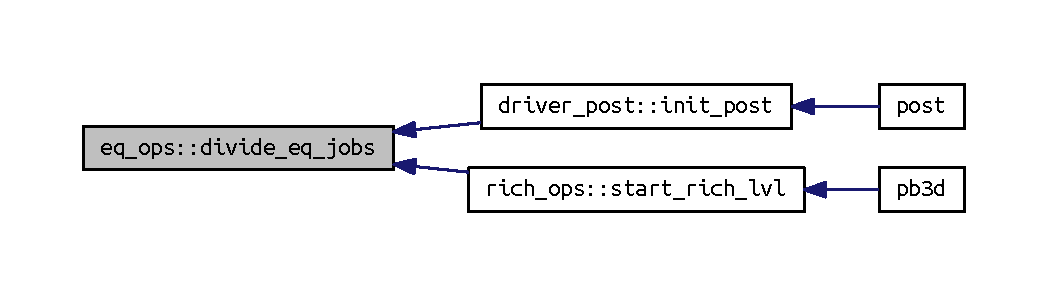
\includegraphics[width=350pt]{namespaceeq__ops_a8fae749abe55865d8135fef536a8e8f1_icgraph}
\end{center}
\end{figure}
\mbox{\Hypertarget{namespaceeq__ops_af0effe20188d46a44680c2648e4572e9}\label{namespaceeq__ops_af0effe20188d46a44680c2648e4572e9}} 
\index{eq\+\_\+ops@{eq\+\_\+ops}!flux\+\_\+q\+\_\+plot@{flux\+\_\+q\+\_\+plot}}
\index{flux\+\_\+q\+\_\+plot@{flux\+\_\+q\+\_\+plot}!eq\+\_\+ops@{eq\+\_\+ops}}
\subsubsection{\texorpdfstring{flux\+\_\+q\+\_\+plot()}{flux\_q\_plot()}}
{\footnotesize\ttfamily integer function, public eq\+\_\+ops\+::flux\+\_\+q\+\_\+plot (\begin{DoxyParamCaption}\item[{type(\hyperlink{structgrid__vars_1_1grid__type}{grid\+\_\+type}), intent(in)}]{grid\+\_\+eq,  }\item[{type(\hyperlink{structeq__vars_1_1eq__1__type}{eq\+\_\+1\+\_\+type}), intent(in)}]{eq }\end{DoxyParamCaption})}



Plots the flux quantities in the solution grid. 


\begin{DoxyItemize}
\item safety factor {\ttfamily q\+\_\+saf} 
\item rotational transform {\ttfamily rot\+\_\+t} 
\item pressure {\ttfamily pres} 
\item poloidal flux {\ttfamily flux\+\_\+p} 
\item toroidal flux {\ttfamily flux\+\_\+t} 
\end{DoxyItemize}

\begin{DoxyReturn}{Returns}
ierr
\end{DoxyReturn}

\begin{DoxyParams}[1]{Parameters}
\mbox{\tt in}  & {\em grid\+\_\+eq} & normal grid\\
\hline
\mbox{\tt in}  & {\em eq} & flux equilibrium variables \\
\hline
\end{DoxyParams}


Definition at line 3757 of file eq\+\_\+ops.\+f90.

Here is the call graph for this function\+:\nopagebreak
\begin{figure}[H]
\begin{center}
\leavevmode
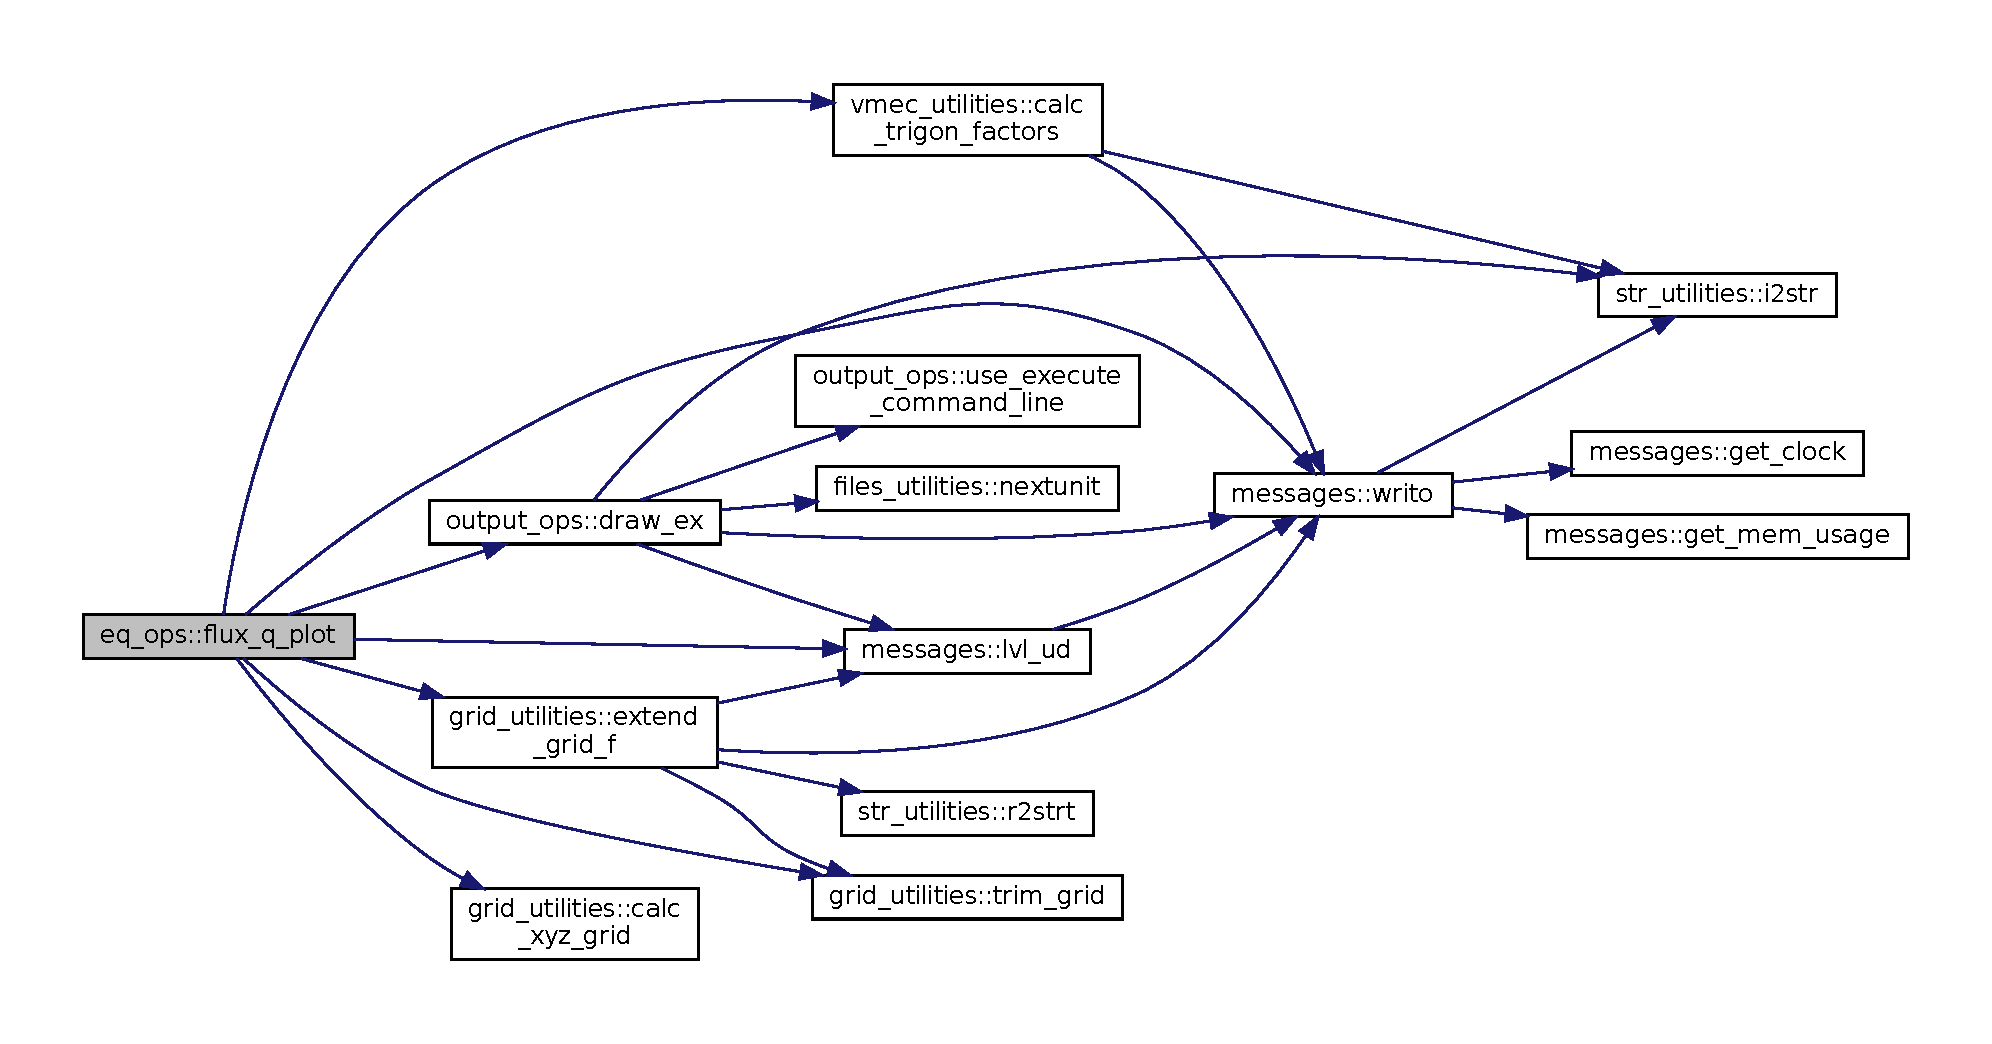
\includegraphics[width=350pt]{namespaceeq__ops_af0effe20188d46a44680c2648e4572e9_cgraph}
\end{center}
\end{figure}
Here is the caller graph for this function\+:\nopagebreak
\begin{figure}[H]
\begin{center}
\leavevmode
\includegraphics[width=350pt]{namespaceeq__ops_af0effe20188d46a44680c2648e4572e9_icgraph}
\end{center}
\end{figure}
\mbox{\Hypertarget{namespaceeq__ops_afabdf28e5c26ceb87e6eb8cf3809919d}\label{namespaceeq__ops_afabdf28e5c26ceb87e6eb8cf3809919d}} 
\index{eq\+\_\+ops@{eq\+\_\+ops}!j\+\_\+plot@{j\+\_\+plot}}
\index{j\+\_\+plot@{j\+\_\+plot}!eq\+\_\+ops@{eq\+\_\+ops}}
\subsubsection{\texorpdfstring{j\+\_\+plot()}{j\_plot()}}
{\footnotesize\ttfamily integer function, public eq\+\_\+ops\+::j\+\_\+plot (\begin{DoxyParamCaption}\item[{type(\hyperlink{structgrid__vars_1_1grid__type}{grid\+\_\+type}), intent(inout)}]{grid\+\_\+eq,  }\item[{type(\hyperlink{structeq__vars_1_1eq__1__type}{eq\+\_\+1\+\_\+type}), intent(in)}]{eq\+\_\+1,  }\item[{type(\hyperlink{structeq__vars_1_1eq__2__type}{eq\+\_\+2\+\_\+type}), intent(in)}]{eq\+\_\+2,  }\item[{integer, intent(in), optional}]{rich\+\_\+lvl,  }\item[{logical, intent(in), optional}]{plot\+\_\+fluxes,  }\item[{real(dp), dimension(\+:,\+:,\+:,\+:), intent(in), optional}]{X\+YZ }\end{DoxyParamCaption})}



Plots the current. 

If multiple equilibrium parallel jobs, every job does its piece, and the results are joined automatically by plot\+\_\+\+H\+D\+F5.

The outputs are given in contra-\/ and covariant components and magnitude in multiple coordinate systems, as indicated in \hyperlink{namespacegrid__utilities_ad3d9386b9abcb1a7e17369a1b3a3750d}{calc\+\_\+vec\+\_\+comp()}.

The starting point is the pressure balance \[ \nabla p = \vec{J} \times \vec{B}, \] which, using $\vec{B} = \frac{\vec{e}_{\theta}}{\mathcal{J}}$, reduces to \[J^\alpha = -p'. \] Furthermore, the current has to lie in the magnetic flux surfaces\+: \[J^\psi = 0. \] Finally, the parallel current $\sigma$ gives an expression for the last contravariant component\+: \[J^\theta = \frac{\sigma}{\mathcal{J}} + p' \frac{B_\alpha}{B_\theta}. \] From these, the contravariant components can be calculated as \[J_i = J^\alpha g_{\alpha,i} + J^\theta g_{\theta,i}. \]

These are then all be transformed to the other coordinate systems. \begin{DoxyNote}{Note}

\begin{DoxyEnumerate}
\item Vector plots for different Richardson levels can be combined to show the total grid by just plotting them all individually.
\item The metric factors and transformation matrices have to be allocated.
\end{DoxyEnumerate}
\end{DoxyNote}
\begin{DoxyReturn}{Returns}
ierr
\end{DoxyReturn}

\begin{DoxyParams}[1]{Parameters}
\mbox{\tt in,out}  & {\em grid\+\_\+eq} & equilibrium grid\\
\hline
\mbox{\tt in}  & {\em eq\+\_\+1} & flux equilibrium variables\\
\hline
\mbox{\tt in}  & {\em eq\+\_\+2} & metric equilibrium variables\\
\hline
\mbox{\tt in}  & {\em rich\+\_\+lvl} & Richardson level\\
\hline
\mbox{\tt in}  & {\em plot\+\_\+fluxes} & plot the fluxes\\
\hline
\mbox{\tt in}  & {\em xyz} & X, Y and Z of grid \\
\hline
\end{DoxyParams}


Definition at line 5157 of file eq\+\_\+ops.\+f90.

Here is the call graph for this function\+:\nopagebreak
\begin{figure}[H]
\begin{center}
\leavevmode
\includegraphics[width=350pt]{namespaceeq__ops_afabdf28e5c26ceb87e6eb8cf3809919d_cgraph}
\end{center}
\end{figure}
Here is the caller graph for this function\+:\nopagebreak
\begin{figure}[H]
\begin{center}
\leavevmode
\includegraphics[width=350pt]{namespaceeq__ops_afabdf28e5c26ceb87e6eb8cf3809919d_icgraph}
\end{center}
\end{figure}
\mbox{\Hypertarget{namespaceeq__ops_ad173efd111cb85c11bc2bc78a7555096}\label{namespaceeq__ops_ad173efd111cb85c11bc2bc78a7555096}} 
\index{eq\+\_\+ops@{eq\+\_\+ops}!kappa\+\_\+plot@{kappa\+\_\+plot}}
\index{kappa\+\_\+plot@{kappa\+\_\+plot}!eq\+\_\+ops@{eq\+\_\+ops}}
\subsubsection{\texorpdfstring{kappa\+\_\+plot()}{kappa\_plot()}}
{\footnotesize\ttfamily integer function, public eq\+\_\+ops\+::kappa\+\_\+plot (\begin{DoxyParamCaption}\item[{type(\hyperlink{structgrid__vars_1_1grid__type}{grid\+\_\+type}), intent(inout)}]{grid\+\_\+eq,  }\item[{type(\hyperlink{structeq__vars_1_1eq__1__type}{eq\+\_\+1\+\_\+type}), intent(in)}]{eq\+\_\+1,  }\item[{type(\hyperlink{structeq__vars_1_1eq__2__type}{eq\+\_\+2\+\_\+type}), intent(in)}]{eq\+\_\+2,  }\item[{integer, intent(in), optional}]{rich\+\_\+lvl,  }\item[{real(dp), dimension(\+:,\+:,\+:,\+:), intent(in), optional}]{X\+YZ }\end{DoxyParamCaption})}



Plots the curvature. 

If multiple equilibrium parallel jobs, every job does its piece, and the results are joined automatically by plot\+\_\+\+H\+D\+F5.

The outputs are given in contra-\/ and covariant components and magnitude in multiple coordinate systems, as indicated in \hyperlink{namespacegrid__utilities_ad3d9386b9abcb1a7e17369a1b3a3750d}{calc\+\_\+vec\+\_\+comp()}.

The starting point is the curvature, given by \[\vec{\kappa} = \kappa_n \frac{\nabla \psi}{ \left|\nabla \psi\right|^2 } + \kappa_g \frac{\nabla \psi \times \vec{B}}{B^2} , \] which can be used to find the covariant and contravariant components in Flux coordinates.

These are then transformed to Cartesian coordinates and plotted.

\begin{DoxyNote}{Note}

\begin{DoxyEnumerate}
\item Vector plots for different Richardson levels can be combined to show the total grid by just plotting them all individually.
\item The metric factors and transformation matrices have to be allocated.
\end{DoxyEnumerate}
\end{DoxyNote}
\begin{DoxyReturn}{Returns}
ierr
\end{DoxyReturn}

\begin{DoxyParams}[1]{Parameters}
\mbox{\tt in,out}  & {\em grid\+\_\+eq} & equilibrium grid\\
\hline
\mbox{\tt in}  & {\em eq\+\_\+1} & metric equilibrium variables\\
\hline
\mbox{\tt in}  & {\em eq\+\_\+2} & metric equilibrium variables\\
\hline
\mbox{\tt in}  & {\em rich\+\_\+lvl} & Richardson level\\
\hline
\mbox{\tt in}  & {\em xyz} & X, Y and Z of grid \\
\hline
\end{DoxyParams}


Definition at line 5325 of file eq\+\_\+ops.\+f90.

Here is the call graph for this function\+:\nopagebreak
\begin{figure}[H]
\begin{center}
\leavevmode
\includegraphics[width=350pt]{namespaceeq__ops_ad173efd111cb85c11bc2bc78a7555096_cgraph}
\end{center}
\end{figure}
Here is the caller graph for this function\+:\nopagebreak
\begin{figure}[H]
\begin{center}
\leavevmode
\includegraphics[width=350pt]{namespaceeq__ops_ad173efd111cb85c11bc2bc78a7555096_icgraph}
\end{center}
\end{figure}
\mbox{\Hypertarget{namespaceeq__ops_a1b4c764da73624722d7e76498a2b80a9}\label{namespaceeq__ops_a1b4c764da73624722d7e76498a2b80a9}} 
\index{eq\+\_\+ops@{eq\+\_\+ops}!normalize\+\_\+input@{normalize\+\_\+input}}
\index{normalize\+\_\+input@{normalize\+\_\+input}!eq\+\_\+ops@{eq\+\_\+ops}}
\subsubsection{\texorpdfstring{normalize\+\_\+input()}{normalize\_input()}}
{\footnotesize\ttfamily subroutine, public eq\+\_\+ops\+::normalize\+\_\+input (\begin{DoxyParamCaption}{ }\end{DoxyParamCaption})}



Normalize input quantities. 

\begin{DoxySeeAlso}{See also}
\hyperlink{namespaceeq__ops_a7cd38586e386e1bc684a327ebcc4c1de}{calc\+\_\+normalization\+\_\+const()} 
\end{DoxySeeAlso}


Definition at line 4997 of file eq\+\_\+ops.\+f90.

Here is the call graph for this function\+:\nopagebreak
\begin{figure}[H]
\begin{center}
\leavevmode
\includegraphics[width=350pt]{namespaceeq__ops_a1b4c764da73624722d7e76498a2b80a9_cgraph}
\end{center}
\end{figure}
Here is the caller graph for this function\+:\nopagebreak
\begin{figure}[H]
\begin{center}
\leavevmode
\includegraphics[width=312pt]{namespaceeq__ops_a1b4c764da73624722d7e76498a2b80a9_icgraph}
\end{center}
\end{figure}
\mbox{\Hypertarget{namespaceeq__ops_a8082c12510696bd8ffdd0deef41860c2}\label{namespaceeq__ops_a8082c12510696bd8ffdd0deef41860c2}} 
\index{eq\+\_\+ops@{eq\+\_\+ops}!test\+\_\+b\+\_\+f@{test\+\_\+b\+\_\+f}}
\index{test\+\_\+b\+\_\+f@{test\+\_\+b\+\_\+f}!eq\+\_\+ops@{eq\+\_\+ops}}
\subsubsection{\texorpdfstring{test\+\_\+b\+\_\+f()}{test\_b\_f()}}
{\footnotesize\ttfamily integer function eq\+\_\+ops\+::test\+\_\+b\+\_\+f (\begin{DoxyParamCaption}\item[{type(\hyperlink{structgrid__vars_1_1grid__type}{grid\+\_\+type}), intent(in)}]{grid\+\_\+eq,  }\item[{type(\hyperlink{structeq__vars_1_1eq__1__type}{eq\+\_\+1\+\_\+type}), intent(in)}]{eq\+\_\+1,  }\item[{type(\hyperlink{structeq__vars_1_1eq__2__type}{eq\+\_\+2\+\_\+type}), intent(in)}]{eq\+\_\+2 }\end{DoxyParamCaption})}



Tests whether $\vec{B}_\text{F}$ is calculated correctly. 

\begin{DoxyNote}{Note}
Debug version only
\end{DoxyNote}
\begin{DoxyReturn}{Returns}
ierr
\end{DoxyReturn}

\begin{DoxyParams}[1]{Parameters}
\mbox{\tt in}  & {\em grid\+\_\+eq} & equilibrium grid\\
\hline
\mbox{\tt in}  & {\em eq\+\_\+1} & flux equilibrium\\
\hline
\mbox{\tt in}  & {\em eq\+\_\+2} & metric equilibrium \\
\hline
\end{DoxyParams}


Definition at line 6698 of file eq\+\_\+ops.\+f90.

Here is the call graph for this function\+:\nopagebreak
\begin{figure}[H]
\begin{center}
\leavevmode
\includegraphics[width=350pt]{namespaceeq__ops_a8082c12510696bd8ffdd0deef41860c2_cgraph}
\end{center}
\end{figure}
Here is the caller graph for this function\+:\nopagebreak
\begin{figure}[H]
\begin{center}
\leavevmode
\includegraphics[width=350pt]{namespaceeq__ops_a8082c12510696bd8ffdd0deef41860c2_icgraph}
\end{center}
\end{figure}
\mbox{\Hypertarget{namespaceeq__ops_a003df1e1ab90dc6f586c3eed3dd067e8}\label{namespaceeq__ops_a003df1e1ab90dc6f586c3eed3dd067e8}} 
\index{eq\+\_\+ops@{eq\+\_\+ops}!test\+\_\+d12h\+\_\+h@{test\+\_\+d12h\+\_\+h}}
\index{test\+\_\+d12h\+\_\+h@{test\+\_\+d12h\+\_\+h}!eq\+\_\+ops@{eq\+\_\+ops}}
\subsubsection{\texorpdfstring{test\+\_\+d12h\+\_\+h()}{test\_d12h\_h()}}
{\footnotesize\ttfamily integer function eq\+\_\+ops\+::test\+\_\+d12h\+\_\+h (\begin{DoxyParamCaption}\item[{type(\hyperlink{structgrid__vars_1_1grid__type}{grid\+\_\+type}), intent(in)}]{grid\+\_\+eq,  }\item[{type(\hyperlink{structeq__vars_1_1eq__2__type}{eq\+\_\+2\+\_\+type}), intent(in)}]{eq }\end{DoxyParamCaption})}



Tests whether $ \frac{\partial^2}{\partial u_i \partial u_j} h_\text{H} $ is calculated correctly. 

\begin{DoxyNote}{Note}
Debug version only
\end{DoxyNote}
\begin{DoxyReturn}{Returns}
ierr
\end{DoxyReturn}

\begin{DoxyParams}[1]{Parameters}
\mbox{\tt in}  & {\em grid\+\_\+eq} & equilibrium grid\\
\hline
\mbox{\tt in}  & {\em eq} & metric equilibrium \\
\hline
\end{DoxyParams}


Definition at line 6307 of file eq\+\_\+ops.\+f90.

Here is the call graph for this function\+:\nopagebreak
\begin{figure}[H]
\begin{center}
\leavevmode
\includegraphics[width=350pt]{namespaceeq__ops_a003df1e1ab90dc6f586c3eed3dd067e8_cgraph}
\end{center}
\end{figure}
Here is the caller graph for this function\+:\nopagebreak
\begin{figure}[H]
\begin{center}
\leavevmode
\includegraphics[width=350pt]{namespaceeq__ops_a003df1e1ab90dc6f586c3eed3dd067e8_icgraph}
\end{center}
\end{figure}
\mbox{\Hypertarget{namespaceeq__ops_a9811c83477d9d85f7401fd7957a590fc}\label{namespaceeq__ops_a9811c83477d9d85f7401fd7957a590fc}} 
\index{eq\+\_\+ops@{eq\+\_\+ops}!test\+\_\+g\+\_\+v@{test\+\_\+g\+\_\+v}}
\index{test\+\_\+g\+\_\+v@{test\+\_\+g\+\_\+v}!eq\+\_\+ops@{eq\+\_\+ops}}
\subsubsection{\texorpdfstring{test\+\_\+g\+\_\+v()}{test\_g\_v()}}
{\footnotesize\ttfamily integer function eq\+\_\+ops\+::test\+\_\+g\+\_\+v (\begin{DoxyParamCaption}\item[{type(\hyperlink{structgrid__vars_1_1grid__type}{grid\+\_\+type}), intent(in)}]{grid\+\_\+eq,  }\item[{type(\hyperlink{structeq__vars_1_1eq__2__type}{eq\+\_\+2\+\_\+type}), intent(in)}]{eq }\end{DoxyParamCaption})}



Tests whether $g_\text{V}$ is calculated correctly. 

\begin{DoxyNote}{Note}
Debug version only
\end{DoxyNote}
\begin{DoxyReturn}{Returns}
ierr
\end{DoxyReturn}

\begin{DoxyParams}[1]{Parameters}
\mbox{\tt in}  & {\em grid\+\_\+eq} & equilibrium grid\\
\hline
\mbox{\tt in}  & {\em eq} & metric equilibrium \\
\hline
\end{DoxyParams}


Definition at line 6535 of file eq\+\_\+ops.\+f90.

Here is the call graph for this function\+:\nopagebreak
\begin{figure}[H]
\begin{center}
\leavevmode
\includegraphics[width=350pt]{namespaceeq__ops_a9811c83477d9d85f7401fd7957a590fc_cgraph}
\end{center}
\end{figure}
Here is the caller graph for this function\+:\nopagebreak
\begin{figure}[H]
\begin{center}
\leavevmode
\includegraphics[width=350pt]{namespaceeq__ops_a9811c83477d9d85f7401fd7957a590fc_icgraph}
\end{center}
\end{figure}
\mbox{\Hypertarget{namespaceeq__ops_a05dcd4803b9c7845d3353614c9630c23}\label{namespaceeq__ops_a05dcd4803b9c7845d3353614c9630c23}} 
\index{eq\+\_\+ops@{eq\+\_\+ops}!test\+\_\+jac\+\_\+f@{test\+\_\+jac\+\_\+f}}
\index{test\+\_\+jac\+\_\+f@{test\+\_\+jac\+\_\+f}!eq\+\_\+ops@{eq\+\_\+ops}}
\subsubsection{\texorpdfstring{test\+\_\+jac\+\_\+f()}{test\_jac\_f()}}
{\footnotesize\ttfamily integer function eq\+\_\+ops\+::test\+\_\+jac\+\_\+f (\begin{DoxyParamCaption}\item[{type(\hyperlink{structgrid__vars_1_1grid__type}{grid\+\_\+type}), intent(in)}]{grid\+\_\+eq,  }\item[{type(\hyperlink{structeq__vars_1_1eq__1__type}{eq\+\_\+1\+\_\+type}), intent(in), target}]{eq\+\_\+1,  }\item[{type(\hyperlink{structeq__vars_1_1eq__2__type}{eq\+\_\+2\+\_\+type}), intent(in)}]{eq\+\_\+2 }\end{DoxyParamCaption})}



Performs tests on $ \mathcal{J}_\text{F}$. 


\begin{DoxyItemize}
\item comparing it with the determinant of $g_\text{F}$
\item comparing it with the direct formula
\end{DoxyItemize}

\begin{DoxyNote}{Note}
Debug version only
\end{DoxyNote}
\begin{DoxyReturn}{Returns}
ierr
\end{DoxyReturn}

\begin{DoxyParams}[1]{Parameters}
\mbox{\tt in}  & {\em grid\+\_\+eq} & equilibrium grid\\
\hline
\mbox{\tt in}  & {\em eq\+\_\+1} & flux equilibrium\\
\hline
\mbox{\tt in}  & {\em eq\+\_\+2} & metric equilibrium \\
\hline
\end{DoxyParams}


Definition at line 6418 of file eq\+\_\+ops.\+f90.

Here is the call graph for this function\+:\nopagebreak
\begin{figure}[H]
\begin{center}
\leavevmode
\includegraphics[width=350pt]{namespaceeq__ops_a05dcd4803b9c7845d3353614c9630c23_cgraph}
\end{center}
\end{figure}
Here is the caller graph for this function\+:\nopagebreak
\begin{figure}[H]
\begin{center}
\leavevmode
\includegraphics[width=350pt]{namespaceeq__ops_a05dcd4803b9c7845d3353614c9630c23_icgraph}
\end{center}
\end{figure}
\mbox{\Hypertarget{namespaceeq__ops_aef40d04e93f6a96576f8fe893fb086f8}\label{namespaceeq__ops_aef40d04e93f6a96576f8fe893fb086f8}} 
\index{eq\+\_\+ops@{eq\+\_\+ops}!test\+\_\+jac\+\_\+v@{test\+\_\+jac\+\_\+v}}
\index{test\+\_\+jac\+\_\+v@{test\+\_\+jac\+\_\+v}!eq\+\_\+ops@{eq\+\_\+ops}}
\subsubsection{\texorpdfstring{test\+\_\+jac\+\_\+v()}{test\_jac\_v()}}
{\footnotesize\ttfamily integer function eq\+\_\+ops\+::test\+\_\+jac\+\_\+v (\begin{DoxyParamCaption}\item[{type(\hyperlink{structgrid__vars_1_1grid__type}{grid\+\_\+type}), intent(in)}]{grid\+\_\+eq,  }\item[{type(\hyperlink{structeq__vars_1_1eq__2__type}{eq\+\_\+2\+\_\+type}), intent(in)}]{eq }\end{DoxyParamCaption})}



Tests whether $\mathcal{J}_\text{V}$ is calculated correctly. 

\begin{DoxyNote}{Note}
Debug version only
\end{DoxyNote}
\begin{DoxyReturn}{Returns}
ierr
\end{DoxyReturn}

\begin{DoxyParams}[1]{Parameters}
\mbox{\tt in}  & {\em grid\+\_\+eq} & equilibrium grid\\
\hline
\mbox{\tt in}  & {\em eq} & metric equilibrium \\
\hline
\end{DoxyParams}


Definition at line 6634 of file eq\+\_\+ops.\+f90.

Here is the call graph for this function\+:\nopagebreak
\begin{figure}[H]
\begin{center}
\leavevmode
\includegraphics[width=350pt]{namespaceeq__ops_aef40d04e93f6a96576f8fe893fb086f8_cgraph}
\end{center}
\end{figure}
Here is the caller graph for this function\+:\nopagebreak
\begin{figure}[H]
\begin{center}
\leavevmode
\includegraphics[width=350pt]{namespaceeq__ops_aef40d04e93f6a96576f8fe893fb086f8_icgraph}
\end{center}
\end{figure}
\mbox{\Hypertarget{namespaceeq__ops_a38b723f6ed5d2e2772c9c3ad14d5ffd4}\label{namespaceeq__ops_a38b723f6ed5d2e2772c9c3ad14d5ffd4}} 
\index{eq\+\_\+ops@{eq\+\_\+ops}!test\+\_\+p@{test\+\_\+p}}
\index{test\+\_\+p@{test\+\_\+p}!eq\+\_\+ops@{eq\+\_\+ops}}
\subsubsection{\texorpdfstring{test\+\_\+p()}{test\_p()}}
{\footnotesize\ttfamily integer function eq\+\_\+ops\+::test\+\_\+p (\begin{DoxyParamCaption}\item[{type(\hyperlink{structgrid__vars_1_1grid__type}{grid\+\_\+type}), intent(in)}]{grid\+\_\+eq,  }\item[{type(\hyperlink{structeq__vars_1_1eq__1__type}{eq\+\_\+1\+\_\+type}), intent(in)}]{eq\+\_\+1,  }\item[{type(\hyperlink{structeq__vars_1_1eq__2__type}{eq\+\_\+2\+\_\+type}), intent(in)}]{eq\+\_\+2 }\end{DoxyParamCaption})}



Performs tests on pressure balance. 

\[\mu_0 \frac{\partial p}{\partial u^2} = \frac{1}{\mathcal{J}} \left(\frac{\partial B_2}{\partial u^3} - \frac{\partial B_3}{\partial u^2}\right)\] \[\mu_0 \mathcal{J} \frac{\partial p}{\partial u^3} = 0 \rightarrow \left(\frac{\partial B_1}{\partial u^3} = \frac{\partial B_3}{\partial u^1}\right), \] working in the (modified) Flux coordinates $\left(\alpha,\psi,\theta\right)_\text{F}$

\begin{DoxyNote}{Note}
Debug version only
\end{DoxyNote}
\begin{DoxyReturn}{Returns}
ierr
\end{DoxyReturn}

\begin{DoxyParams}[1]{Parameters}
\mbox{\tt in}  & {\em grid\+\_\+eq} & equilibrium grid\\
\hline
\mbox{\tt in}  & {\em eq\+\_\+1} & flux equilibrium variables\\
\hline
\mbox{\tt in}  & {\em eq\+\_\+2} & metric equilibrium variables \\
\hline
\end{DoxyParams}


Definition at line 6856 of file eq\+\_\+ops.\+f90.

Here is the call graph for this function\+:\nopagebreak
\begin{figure}[H]
\begin{center}
\leavevmode
\includegraphics[width=350pt]{namespaceeq__ops_a38b723f6ed5d2e2772c9c3ad14d5ffd4_cgraph}
\end{center}
\end{figure}
Here is the caller graph for this function\+:\nopagebreak
\begin{figure}[H]
\begin{center}
\leavevmode
\includegraphics[width=350pt]{namespaceeq__ops_a38b723f6ed5d2e2772c9c3ad14d5ffd4_icgraph}
\end{center}
\end{figure}
\mbox{\Hypertarget{namespaceeq__ops_a1f5049c3e309fa23ee46fd116c9344f1}\label{namespaceeq__ops_a1f5049c3e309fa23ee46fd116c9344f1}} 
\index{eq\+\_\+ops@{eq\+\_\+ops}!test\+\_\+t\+\_\+ef@{test\+\_\+t\+\_\+ef}}
\index{test\+\_\+t\+\_\+ef@{test\+\_\+t\+\_\+ef}!eq\+\_\+ops@{eq\+\_\+ops}}
\subsubsection{\texorpdfstring{test\+\_\+t\+\_\+ef()}{test\_t\_ef()}}
{\footnotesize\ttfamily integer function eq\+\_\+ops\+::test\+\_\+t\+\_\+ef (\begin{DoxyParamCaption}\item[{type(\hyperlink{structgrid__vars_1_1grid__type}{grid\+\_\+type}), intent(in)}]{grid\+\_\+eq,  }\item[{type(\hyperlink{structeq__vars_1_1eq__1__type}{eq\+\_\+1\+\_\+type}), intent(in)}]{eq\+\_\+1,  }\item[{type(\hyperlink{structeq__vars_1_1eq__2__type}{eq\+\_\+2\+\_\+type}), intent(in)}]{eq\+\_\+2 }\end{DoxyParamCaption})}



See if {\ttfamily T\+\_\+\+EF} it complies with the theory of \cite{Weyens3D}. 

\begin{DoxyNote}{Note}
Debug version only
\end{DoxyNote}
\begin{DoxyReturn}{Returns}
ierr
\end{DoxyReturn}

\begin{DoxyParams}[1]{Parameters}
\mbox{\tt in}  & {\em grid\+\_\+eq} & equilibrium grid\\
\hline
\mbox{\tt in}  & {\em eq\+\_\+1} & flux equilibrium\\
\hline
\mbox{\tt in}  & {\em eq\+\_\+2} & metric equilibrium \\
\hline
\end{DoxyParams}


Definition at line 6133 of file eq\+\_\+ops.\+f90.

Here is the call graph for this function\+:\nopagebreak
\begin{figure}[H]
\begin{center}
\leavevmode
\includegraphics[width=350pt]{namespaceeq__ops_a1f5049c3e309fa23ee46fd116c9344f1_cgraph}
\end{center}
\end{figure}
Here is the caller graph for this function\+:\nopagebreak
\begin{figure}[H]
\begin{center}
\leavevmode
\includegraphics[width=350pt]{namespaceeq__ops_a1f5049c3e309fa23ee46fd116c9344f1_icgraph}
\end{center}
\end{figure}


\subsection{Variable Documentation}
\mbox{\Hypertarget{namespaceeq__ops_a1b6609a8d8b427d9133bf323e732f209}\label{namespaceeq__ops_a1b6609a8d8b427d9133bf323e732f209}} 
\index{eq\+\_\+ops@{eq\+\_\+ops}!debug\+\_\+calc\+\_\+derived\+\_\+q@{debug\+\_\+calc\+\_\+derived\+\_\+q}}
\index{debug\+\_\+calc\+\_\+derived\+\_\+q@{debug\+\_\+calc\+\_\+derived\+\_\+q}!eq\+\_\+ops@{eq\+\_\+ops}}
\subsubsection{\texorpdfstring{debug\+\_\+calc\+\_\+derived\+\_\+q}{debug\_calc\_derived\_q}}
{\footnotesize\ttfamily logical, public eq\+\_\+ops\+::debug\+\_\+calc\+\_\+derived\+\_\+q = .false.}



plot debug information for \hyperlink{namespaceeq__ops_a087e08ce6d8ad381b5bac8fc51148d50}{calc\+\_\+derived\+\_\+q()} 

\begin{DoxyNote}{Note}
Debug version only 
\end{DoxyNote}


Definition at line 30 of file eq\+\_\+ops.\+f90.

\mbox{\Hypertarget{namespaceeq__ops_a07ca60790a262e20bc8632be1530970a}\label{namespaceeq__ops_a07ca60790a262e20bc8632be1530970a}} 
\index{eq\+\_\+ops@{eq\+\_\+ops}!debug\+\_\+create\+\_\+vmec\+\_\+input@{debug\+\_\+create\+\_\+vmec\+\_\+input}}
\index{debug\+\_\+create\+\_\+vmec\+\_\+input@{debug\+\_\+create\+\_\+vmec\+\_\+input}!eq\+\_\+ops@{eq\+\_\+ops}}
\subsubsection{\texorpdfstring{debug\+\_\+create\+\_\+vmec\+\_\+input}{debug\_create\_vmec\_input}}
{\footnotesize\ttfamily logical, public eq\+\_\+ops\+::debug\+\_\+create\+\_\+vmec\+\_\+input = .false.}



plot debug information for \hyperlink{namespaceeq__ops_a9addef683b3d4a8c587510e4c994ec61}{create\+\_\+vmec\+\_\+input()} 

\begin{DoxyNote}{Note}
Debug version only 
\end{DoxyNote}


Definition at line 34 of file eq\+\_\+ops.\+f90.

\mbox{\Hypertarget{namespaceeq__ops_a45ba7f46fd439bbd73edfd1fd548b58e}\label{namespaceeq__ops_a45ba7f46fd439bbd73edfd1fd548b58e}} 
\index{eq\+\_\+ops@{eq\+\_\+ops}!debug\+\_\+j\+\_\+plot@{debug\+\_\+j\+\_\+plot}}
\index{debug\+\_\+j\+\_\+plot@{debug\+\_\+j\+\_\+plot}!eq\+\_\+ops@{eq\+\_\+ops}}
\subsubsection{\texorpdfstring{debug\+\_\+j\+\_\+plot}{debug\_j\_plot}}
{\footnotesize\ttfamily logical, public eq\+\_\+ops\+::debug\+\_\+j\+\_\+plot = .false.}



plot debug information for \hyperlink{namespaceeq__ops_afabdf28e5c26ceb87e6eb8cf3809919d}{j\+\_\+plot()} 

\begin{DoxyNote}{Note}
Debug version only 
\end{DoxyNote}


Definition at line 32 of file eq\+\_\+ops.\+f90.


\hypertarget{namespaceeq__utilities}{}\doxysection{eq\+\_\+utilities Module Reference}
\label{namespaceeq__utilities}\index{eq\_utilities@{eq\_utilities}}


Numerical utilities related to equilibrium variables.  


\doxysubsection*{Interfaces and Types}
\begin{DoxyCompactItemize}
\item 
interface \mbox{\hyperlink{interfaceeq__utilities_1_1calc__f__derivs}{calc\+\_\+f\+\_\+derivs}}
\begin{DoxyCompactList}\small\item\em Transforms derivatives of the equilibrium quantities in E coordinates to derivatives in the F coordinates. \end{DoxyCompactList}\item 
interface \mbox{\hyperlink{interfaceeq__utilities_1_1calc__inv__met}{calc\+\_\+inv\+\_\+met}}
\begin{DoxyCompactList}\small\item\em Calculate $D_1^{m_1} D_2^{m_2} D_3^{m_3} X$ from $D_1^{i_1} D_2^{i_2} D_3^{i_3} X$ and $D_1^{j_1} D_2^{j_2} D_3^{j_3} Y$ where $XY=1$ and $i,j = 0\ldots m$, according to \cite{Weyens3D}. \end{DoxyCompactList}\item 
interface \mbox{\hyperlink{interfaceeq__utilities_1_1transf__deriv}{transf\+\_\+deriv}}
\begin{DoxyCompactList}\small\item\em Calculates derivatives in a coordinate system B from derivatives in a coordinates system A, making use of the transformation matrix $\overline{\text{T}}_\text{B}^\text{A}$. \end{DoxyCompactList}\end{DoxyCompactItemize}
\doxysubsection*{Functions/\+Subroutines}
\begin{DoxyCompactItemize}
\item 
integer function, public \mbox{\hyperlink{namespaceeq__utilities_a1426f7226577f8719472265fd882fbf4}{calc\+\_\+g}} (g\+\_\+A, T\+\_\+\+BA, g\+\_\+B, deriv, max\+\_\+deriv)
\begin{DoxyCompactList}\small\item\em Calculate the metric coefficients in a coordinate system B ! using the. \end{DoxyCompactList}\item 
integer function, public \mbox{\hyperlink{namespaceeq__utilities_a5a9f230ed9a6e627e31e882e9f4a00a1}{calc\+\_\+memory\+\_\+eq}} (arr\+\_\+size, n\+\_\+par, mem\+\_\+size)
\begin{DoxyCompactList}\small\item\em Calculate memory in MB necessary for variables in equilibrium job. \end{DoxyCompactList}\item 
logical function, public \mbox{\hyperlink{namespaceeq__utilities_a5109472305101af3a15e8e8717c426fd}{do\+\_\+eq}} ()
\begin{DoxyCompactList}\small\item\em If this equilibrium job should be done, also increment {\ttfamily eq\+\_\+job\+\_\+nr}. \end{DoxyCompactList}\item 
elemental character(len=max\+\_\+str\+\_\+ln) function, public \mbox{\hyperlink{namespaceeq__utilities_a34c5ddab45a54a6c738e5e0b8c7d55d6}{eq\+\_\+info}} ()
\begin{DoxyCompactList}\small\item\em Returns string with possible extension with equilibrium job as well as parallel job, or nothing if only one level and one parallel job. \end{DoxyCompactList}\item 
subroutine, public \mbox{\hyperlink{namespaceeq__utilities_a40f397d20b45432117744ca16870ddbb}{print\+\_\+info\+\_\+eq}} (n\+\_\+par\+\_\+\+X\+\_\+rich)
\begin{DoxyCompactList}\small\item\em Prints information for equilibrium parallel job. \end{DoxyCompactList}\end{DoxyCompactItemize}
\doxysubsection*{Variables}
\begin{DoxyCompactItemize}
\item 
logical, public \mbox{\hyperlink{namespaceeq__utilities_aedf0e1858d0bd16218a290f4857d416a}{debug\+\_\+calc\+\_\+inv\+\_\+met\+\_\+ind}} = .false.
\begin{DoxyCompactList}\small\item\em plot debug information for calc\+\_\+inv\+\_\+met\+\_\+ind() \end{DoxyCompactList}\end{DoxyCompactItemize}


\doxysubsection{Detailed Description}
Numerical utilities related to equilibrium variables. 

\doxysubsection{Function/\+Subroutine Documentation}
\mbox{\Hypertarget{namespaceeq__utilities_a1426f7226577f8719472265fd882fbf4}\label{namespaceeq__utilities_a1426f7226577f8719472265fd882fbf4}} 
\index{eq\_utilities@{eq\_utilities}!calc\_g@{calc\_g}}
\index{calc\_g@{calc\_g}!eq\_utilities@{eq\_utilities}}
\doxysubsubsection{\texorpdfstring{calc\_g()}{calc\_g()}}
{\footnotesize\ttfamily integer function, public eq\+\_\+utilities\+::calc\+\_\+g (\begin{DoxyParamCaption}\item[{real(dp), dimension(\+:,\+:,\+:,\+:,0\+:,0\+:,0\+:), intent(in)}]{g\+\_\+A,  }\item[{real(dp), dimension(\+:,\+:,\+:,\+:,0\+:,0\+:,0\+:), intent(in)}]{T\+\_\+\+BA,  }\item[{real(dp), dimension(\+:,\+:,\+:,\+:,0\+:,0\+:,0\+:), intent(inout)}]{g\+\_\+B,  }\item[{integer, dimension(3), intent(in)}]{deriv,  }\item[{integer, intent(in)}]{max\+\_\+deriv }\end{DoxyParamCaption})}



Calculate the metric coefficients in a coordinate system B ! using the. 


\begin{DoxyParams}[1]{Parameters}
\mbox{\texttt{ in}}  & {\em g\+\_\+a} & $g_\text{A}$ \\
\hline
\mbox{\texttt{ in}}  & {\em t\+\_\+ba} & $\overline{\text{T}}_\text{B}^\text{A}$ \\
\hline
\mbox{\texttt{ in,out}}  & {\em g\+\_\+b} & $g_\text{B}$ \\
\hline
\mbox{\texttt{ in}}  & {\em deriv} & derivatives \\
\hline
\mbox{\texttt{ in}}  & {\em max\+\_\+deriv} & maximum derivative \\
\hline
\end{DoxyParams}


Definition at line 387 of file eq\+\_\+utilities.\+f90.

Here is the caller graph for this function\+:\nopagebreak
\begin{figure}[H]
\begin{center}
\leavevmode
\includegraphics[width=350pt]{namespaceeq__utilities_a1426f7226577f8719472265fd882fbf4_icgraph}
\end{center}
\end{figure}
\mbox{\Hypertarget{namespaceeq__utilities_a5a9f230ed9a6e627e31e882e9f4a00a1}\label{namespaceeq__utilities_a5a9f230ed9a6e627e31e882e9f4a00a1}} 
\index{eq\_utilities@{eq\_utilities}!calc\_memory\_eq@{calc\_memory\_eq}}
\index{calc\_memory\_eq@{calc\_memory\_eq}!eq\_utilities@{eq\_utilities}}
\doxysubsubsection{\texorpdfstring{calc\_memory\_eq()}{calc\_memory\_eq()}}
{\footnotesize\ttfamily integer function, public eq\+\_\+utilities\+::calc\+\_\+memory\+\_\+eq (\begin{DoxyParamCaption}\item[{integer, intent(in)}]{arr\+\_\+size,  }\item[{integer, intent(in)}]{n\+\_\+par,  }\item[{real(dp), intent(inout)}]{mem\+\_\+size }\end{DoxyParamCaption})}



Calculate memory in MB necessary for variables in equilibrium job. 

The size of these variables is equal to the product of the non-\/parallel dimensions (e.\+g. {\ttfamily n\+\_\+geo} x {\ttfamily loc\+\_\+n\+\_\+r}), times the number of variables.

The latter should be\+:
\begin{DoxyItemize}
\item P\+B3D\+: only take into account ( $2\cdot6+1 = 13$) equilibrium variables {\ttfamily g\+\_\+\+FD}, {\ttfamily h\+\_\+\+FD} and {\ttfamily jac\+\_\+\+FD}, as the perturbation variables are divided in jobs occupying the remaning space. These equilibrium variables are tabulated on the equilibrium grid. Note that they contain derivatives in extra dimensions, so that their size should be multiplied by ({\ttfamily max\+\_\+deriv+1})$^\wedge$3.
\item P\+O\+ST\+: take into account these 13 equilibrium variables, as well as 4 variables {\ttfamily U} and {\ttfamily DU}, with double size due to being complex, and the additional dimension equal to {\ttfamily n\+\_\+mod\+\_\+X}, but without derivatives.
\end{DoxyItemize}

\begin{DoxyReturn}{Returns}
ierr 
\end{DoxyReturn}

\begin{DoxyParams}[1]{Parameters}
\mbox{\texttt{ in}}  & {\em arr\+\_\+size} & size of part of X array \\
\hline
\mbox{\texttt{ in}}  & {\em n\+\_\+par} & number of parallel points \\
\hline
\mbox{\texttt{ in,out}}  & {\em mem\+\_\+size} & total size \\
\hline
\end{DoxyParams}


Definition at line 907 of file eq\+\_\+utilities.\+f90.

Here is the caller graph for this function\+:\nopagebreak
\begin{figure}[H]
\begin{center}
\leavevmode
\includegraphics[width=350pt]{namespaceeq__utilities_a5a9f230ed9a6e627e31e882e9f4a00a1_icgraph}
\end{center}
\end{figure}
\mbox{\Hypertarget{namespaceeq__utilities_a5109472305101af3a15e8e8717c426fd}\label{namespaceeq__utilities_a5109472305101af3a15e8e8717c426fd}} 
\index{eq\_utilities@{eq\_utilities}!do\_eq@{do\_eq}}
\index{do\_eq@{do\_eq}!eq\_utilities@{eq\_utilities}}
\doxysubsubsection{\texorpdfstring{do\_eq()}{do\_eq()}}
{\footnotesize\ttfamily logical function, public eq\+\_\+utilities\+::do\+\_\+eq}



If this equilibrium job should be done, also increment {\ttfamily eq\+\_\+job\+\_\+nr}. 



Definition at line 949 of file eq\+\_\+utilities.\+f90.

Here is the caller graph for this function\+:\nopagebreak
\begin{figure}[H]
\begin{center}
\leavevmode
\includegraphics[width=286pt]{namespaceeq__utilities_a5109472305101af3a15e8e8717c426fd_icgraph}
\end{center}
\end{figure}
\mbox{\Hypertarget{namespaceeq__utilities_a34c5ddab45a54a6c738e5e0b8c7d55d6}\label{namespaceeq__utilities_a34c5ddab45a54a6c738e5e0b8c7d55d6}} 
\index{eq\_utilities@{eq\_utilities}!eq\_info@{eq\_info}}
\index{eq\_info@{eq\_info}!eq\_utilities@{eq\_utilities}}
\doxysubsubsection{\texorpdfstring{eq\_info()}{eq\_info()}}
{\footnotesize\ttfamily elemental character(len=max\+\_\+str\+\_\+ln) function, public eq\+\_\+utilities\+::eq\+\_\+info}



Returns string with possible extension with equilibrium job as well as parallel job, or nothing if only one level and one parallel job. 



Definition at line 974 of file eq\+\_\+utilities.\+f90.

Here is the caller graph for this function\+:\nopagebreak
\begin{figure}[H]
\begin{center}
\leavevmode
\includegraphics[width=294pt]{namespaceeq__utilities_a34c5ddab45a54a6c738e5e0b8c7d55d6_icgraph}
\end{center}
\end{figure}
\mbox{\Hypertarget{namespaceeq__utilities_a40f397d20b45432117744ca16870ddbb}\label{namespaceeq__utilities_a40f397d20b45432117744ca16870ddbb}} 
\index{eq\_utilities@{eq\_utilities}!print\_info\_eq@{print\_info\_eq}}
\index{print\_info\_eq@{print\_info\_eq}!eq\_utilities@{eq\_utilities}}
\doxysubsubsection{\texorpdfstring{print\_info\_eq()}{print\_info\_eq()}}
{\footnotesize\ttfamily subroutine, public eq\+\_\+utilities\+::print\+\_\+info\+\_\+eq (\begin{DoxyParamCaption}\item[{integer, intent(in)}]{n\+\_\+par\+\_\+\+X\+\_\+rich }\end{DoxyParamCaption})}



Prints information for equilibrium parallel job. 


\begin{DoxyParams}[1]{Parameters}
\mbox{\texttt{ in}}  & {\em n\+\_\+par\+\_\+x\+\_\+rich} & number of parallel points in this Richardson level \\
\hline
\end{DoxyParams}


Definition at line 986 of file eq\+\_\+utilities.\+f90.

Here is the caller graph for this function\+:\nopagebreak
\begin{figure}[H]
\begin{center}
\leavevmode
\includegraphics[width=350pt]{namespaceeq__utilities_a40f397d20b45432117744ca16870ddbb_icgraph}
\end{center}
\end{figure}


\doxysubsection{Variable Documentation}
\mbox{\Hypertarget{namespaceeq__utilities_aedf0e1858d0bd16218a290f4857d416a}\label{namespaceeq__utilities_aedf0e1858d0bd16218a290f4857d416a}} 
\index{eq\_utilities@{eq\_utilities}!debug\_calc\_inv\_met\_ind@{debug\_calc\_inv\_met\_ind}}
\index{debug\_calc\_inv\_met\_ind@{debug\_calc\_inv\_met\_ind}!eq\_utilities@{eq\_utilities}}
\doxysubsubsection{\texorpdfstring{debug\_calc\_inv\_met\_ind}{debug\_calc\_inv\_met\_ind}}
{\footnotesize\ttfamily logical, public eq\+\_\+utilities\+::debug\+\_\+calc\+\_\+inv\+\_\+met\+\_\+ind = .false.}



plot debug information for calc\+\_\+inv\+\_\+met\+\_\+ind() 

\begin{DoxyNote}{Note}
Debug version only 
\end{DoxyNote}


Definition at line 27 of file eq\+\_\+utilities.\+f90.


\hypertarget{namespaceeq__vars}{}\section{eq\+\_\+vars Module Reference}
\label{namespaceeq__vars}\index{eq\+\_\+vars@{eq\+\_\+vars}}


Variables that have to do with equilibrium quantities and the grid used in the calculations\+:  


\subsection*{Interfaces and Types}
\begin{DoxyCompactItemize}
\item 
type \hyperlink{structeq__vars_1_1eq__1__type}{eq\+\_\+1\+\_\+type}
\begin{DoxyCompactList}\small\item\em flux equilibrium type \end{DoxyCompactList}\item 
type \hyperlink{structeq__vars_1_1eq__2__type}{eq\+\_\+2\+\_\+type}
\begin{DoxyCompactList}\small\item\em metric equilibrium type \end{DoxyCompactList}\end{DoxyCompactItemize}
\subsection*{Functions/\+Subroutines}
\begin{DoxyCompactItemize}
\item 
subroutine \hyperlink{namespaceeq__vars_a0270785c6b513c53e6d7c837f38f377b}{init\+\_\+eq\+\_\+1} (eq, grid, setup\+\_\+E, setup\+\_\+F)
\begin{DoxyCompactList}\small\item\em Initializes new flux equilibrium. \end{DoxyCompactList}\item 
subroutine \hyperlink{namespaceeq__vars_a93947b772250ef73b25bde7688b33bc2}{init\+\_\+eq\+\_\+2} (eq, grid, setup\+\_\+E, setup\+\_\+F)
\begin{DoxyCompactList}\small\item\em Initializes new metric equilibrium. \end{DoxyCompactList}\item 
subroutine \hyperlink{namespaceeq__vars_aa781ffa18b6b17905e126871c43d3267}{copy\+\_\+eq\+\_\+1} (eq\+\_\+i, grid\+\_\+i, eq\+\_\+o)
\begin{DoxyCompactList}\small\item\em Deep copy of flux equilibrium variables. \end{DoxyCompactList}\item 
subroutine \hyperlink{namespaceeq__vars_a50561f7dcd43970bd16a31cd87714c12}{copy\+\_\+eq\+\_\+2} (eq\+\_\+i, grid\+\_\+i, eq\+\_\+o)
\begin{DoxyCompactList}\small\item\em Deep copy of metric equilibrium variables. \end{DoxyCompactList}\item 
subroutine \hyperlink{namespaceeq__vars_ab106dc007ddc896092d0464233b3ce12}{dealloc\+\_\+eq\+\_\+1} (eq)
\begin{DoxyCompactList}\small\item\em Deallocates flux equilibrium quantities. \end{DoxyCompactList}\item 
subroutine \hyperlink{namespaceeq__vars_a206698a627df7d8285921ee4a9f75c11}{dealloc\+\_\+eq\+\_\+2} (eq)
\begin{DoxyCompactList}\small\item\em Deallocates metric equilibrium quantities. \end{DoxyCompactList}\end{DoxyCompactItemize}
\subsection*{Variables}
\begin{DoxyCompactItemize}
\item 
real(dp), public \hyperlink{namespaceeq__vars_a0c1f124ab3260a0f6937df9189a18184}{r\+\_\+0}
\begin{DoxyCompactList}\small\item\em independent normalization constant for nondimensionalization \end{DoxyCompactList}\item 
real(dp), public \hyperlink{namespaceeq__vars_abce8bbe23c333a591a2ee5cef9512de9}{pres\+\_\+0}
\begin{DoxyCompactList}\small\item\em independent normalization constant for nondimensionalization \end{DoxyCompactList}\item 
real(dp), public \hyperlink{namespaceeq__vars_a8c9bdb18a418329b9be241342ea704e3}{rho\+\_\+0}
\begin{DoxyCompactList}\small\item\em independent normalization constant for nondimensionalization \end{DoxyCompactList}\item 
real(dp), public \hyperlink{namespaceeq__vars_acdd2464f2282359a818e4159b502e84b}{b\+\_\+0}
\begin{DoxyCompactList}\small\item\em derived normalization constant for nondimensionalization \end{DoxyCompactList}\item 
real(dp), public \hyperlink{namespaceeq__vars_a2bb2594492faa83869c3eaf8cabe521e}{psi\+\_\+0}
\begin{DoxyCompactList}\small\item\em derived normalization constant for nondimensionalization \end{DoxyCompactList}\item 
real(dp), public \hyperlink{namespaceeq__vars_a5170d0b84bb0faf24d5fdcf7c9371620}{t\+\_\+0}
\begin{DoxyCompactList}\small\item\em derived normalization constant for nondimensionalization \end{DoxyCompactList}\item 
real(dp), public \hyperlink{namespaceeq__vars_ac45a3781896236d8c8fe95d920f7337c}{vac\+\_\+perm} = mu\+\_\+0\+\_\+original
\begin{DoxyCompactList}\small\item\em either usual mu\+\_\+0 (default) or normalized \end{DoxyCompactList}\item 
real(dp), public \hyperlink{namespaceeq__vars_a863feef76ae60309d2e3ed4eed6bd436}{max\+\_\+flux\+\_\+e}
\begin{DoxyCompactList}\small\item\em max. flux in Equilibrium coordinates, set in calc\+\_\+norm\+\_\+range\+\_\+\+P\+B3\+D\+\_\+in \end{DoxyCompactList}\item 
real(dp), public \hyperlink{namespaceeq__vars_a46c97bf2a6d6eca952ca5173fcf9cdcb}{max\+\_\+flux\+\_\+f}
\begin{DoxyCompactList}\small\item\em max. flux in Flux coordinates, set in calc\+\_\+norm\+\_\+range\+\_\+\+P\+B3\+D\+\_\+in \end{DoxyCompactList}\item 
integer, public \hyperlink{namespaceeq__vars_aed1853ac20f0da0be39ab8ef82993c4d}{n\+\_\+alloc\+\_\+eq\+\_\+1s}
\begin{DoxyCompactList}\small\item\em nr. of allocated {\ttfamily eq\+\_\+1} variables \end{DoxyCompactList}\item 
integer, public \hyperlink{namespaceeq__vars_af75297445b32de13371da989074dd454}{n\+\_\+alloc\+\_\+eq\+\_\+2s}
\begin{DoxyCompactList}\small\item\em nr. of allocated {\ttfamily eq\+\_\+2} variables \end{DoxyCompactList}\end{DoxyCompactItemize}


\subsection{Detailed Description}
Variables that have to do with equilibrium quantities and the grid used in the calculations\+: 


\begin{DoxyItemize}
\item The equilibrium variables are comprised of the variables that result from the equilibrium calculation, such as pressure, rotational transform, etc.
\item The flux variables are tabulated on a 1D grid.
\item The metric variables are tabulated on a 3D grid
\begin{DoxyItemize}
\item In the normal coordinate, they are tabulated in the equilibrium grid.
\item In the angular coordinates, they are tabulated in the solution grid (V\+M\+EC), or in the equilibrium grid followed by an adaptation to the solution grid (H\+E\+L\+E\+NA).
\end{DoxyItemize}
\item However, this is not necessarily always the case, as it depends on the grid angles being aligned with the grid (e.\+g. Providing theta and zeta in the equilibrium grid so that the magnetic field lines are followed.
\end{DoxyItemize}

\begin{DoxyNote}{Note}
In general in P\+B3D, there are two kinds of variables, differing from one another in the way in which they are tabulated\+:
\begin{DoxyItemize}
\item variables tabulated on the full output grid of the equilibrium code
\item variables tabulated in an internal grid of this code 
\end{DoxyItemize}

In many places in the code a range in the normal coordinate is selected for each of the variables on different processes. This selection has to be done correctly and things can get a little bit complicated if trimmed grids are used (grids that have no overlap between processes).
\end{DoxyNote}
\begin{DoxySeeAlso}{See also}
grid\+\_\+ops() 
\end{DoxySeeAlso}


\subsection{Function/\+Subroutine Documentation}
\mbox{\Hypertarget{namespaceeq__vars_aa781ffa18b6b17905e126871c43d3267}\label{namespaceeq__vars_aa781ffa18b6b17905e126871c43d3267}} 
\index{eq\+\_\+vars@{eq\+\_\+vars}!copy\+\_\+eq\+\_\+1@{copy\+\_\+eq\+\_\+1}}
\index{copy\+\_\+eq\+\_\+1@{copy\+\_\+eq\+\_\+1}!eq\+\_\+vars@{eq\+\_\+vars}}
\subsubsection{\texorpdfstring{copy\+\_\+eq\+\_\+1()}{copy\_eq\_1()}}
{\footnotesize\ttfamily subroutine eq\+\_\+vars\+::copy\+\_\+eq\+\_\+1 (\begin{DoxyParamCaption}\item[{class(\hyperlink{structeq__vars_1_1eq__1__type}{eq\+\_\+1\+\_\+type}), intent(in)}]{eq\+\_\+i,  }\item[{type(\hyperlink{structgrid__vars_1_1grid__type}{grid\+\_\+type}), intent(in)}]{grid\+\_\+i,  }\item[{type(\hyperlink{structeq__vars_1_1eq__1__type}{eq\+\_\+1\+\_\+type}), intent(inout)}]{eq\+\_\+o }\end{DoxyParamCaption})}



Deep copy of flux equilibrium variables. 


\begin{DoxyParams}[1]{Parameters}
\mbox{\tt in}  & {\em eq\+\_\+i} & eq\+\_\+1 to be copied\\
\hline
\mbox{\tt in}  & {\em grid\+\_\+i} & grid of eq\+\_\+i\\
\hline
\mbox{\tt in,out}  & {\em eq\+\_\+o} & copied eq\+\_\+1 \\
\hline
\end{DoxyParams}


Definition at line 439 of file eq\+\_\+vars.\+f90.

\mbox{\Hypertarget{namespaceeq__vars_a50561f7dcd43970bd16a31cd87714c12}\label{namespaceeq__vars_a50561f7dcd43970bd16a31cd87714c12}} 
\index{eq\+\_\+vars@{eq\+\_\+vars}!copy\+\_\+eq\+\_\+2@{copy\+\_\+eq\+\_\+2}}
\index{copy\+\_\+eq\+\_\+2@{copy\+\_\+eq\+\_\+2}!eq\+\_\+vars@{eq\+\_\+vars}}
\subsubsection{\texorpdfstring{copy\+\_\+eq\+\_\+2()}{copy\_eq\_2()}}
{\footnotesize\ttfamily subroutine eq\+\_\+vars\+::copy\+\_\+eq\+\_\+2 (\begin{DoxyParamCaption}\item[{class(\hyperlink{structeq__vars_1_1eq__2__type}{eq\+\_\+2\+\_\+type}), intent(in)}]{eq\+\_\+i,  }\item[{type(\hyperlink{structgrid__vars_1_1grid__type}{grid\+\_\+type}), intent(in)}]{grid\+\_\+i,  }\item[{type(\hyperlink{structeq__vars_1_1eq__2__type}{eq\+\_\+2\+\_\+type}), intent(inout)}]{eq\+\_\+o }\end{DoxyParamCaption})}



Deep copy of metric equilibrium variables. 

\begin{DoxyReturn}{Returns}
ierr
\end{DoxyReturn}

\begin{DoxyParams}[1]{Parameters}
\mbox{\tt in}  & {\em eq\+\_\+i} & eq\+\_\+2 to be copied\\
\hline
\mbox{\tt in}  & {\em grid\+\_\+i} & grid of eq\+\_\+i\\
\hline
\mbox{\tt in,out}  & {\em eq\+\_\+o} & copied eq\+\_\+1 \\
\hline
\end{DoxyParams}


Definition at line 477 of file eq\+\_\+vars.\+f90.

\mbox{\Hypertarget{namespaceeq__vars_ab106dc007ddc896092d0464233b3ce12}\label{namespaceeq__vars_ab106dc007ddc896092d0464233b3ce12}} 
\index{eq\+\_\+vars@{eq\+\_\+vars}!dealloc\+\_\+eq\+\_\+1@{dealloc\+\_\+eq\+\_\+1}}
\index{dealloc\+\_\+eq\+\_\+1@{dealloc\+\_\+eq\+\_\+1}!eq\+\_\+vars@{eq\+\_\+vars}}
\subsubsection{\texorpdfstring{dealloc\+\_\+eq\+\_\+1()}{dealloc\_eq\_1()}}
{\footnotesize\ttfamily subroutine eq\+\_\+vars\+::dealloc\+\_\+eq\+\_\+1 (\begin{DoxyParamCaption}\item[{class(\hyperlink{structeq__vars_1_1eq__1__type}{eq\+\_\+1\+\_\+type}), intent(inout)}]{eq }\end{DoxyParamCaption})}



Deallocates flux equilibrium quantities. 


\begin{DoxyParams}[1]{Parameters}
\mbox{\tt in,out}  & {\em eq} & equilibrium to be deallocated \\
\hline
\end{DoxyParams}


Definition at line 531 of file eq\+\_\+vars.\+f90.

Here is the call graph for this function\+:\nopagebreak
\begin{figure}[H]
\begin{center}
\leavevmode
\includegraphics[width=350pt]{namespaceeq__vars_ab106dc007ddc896092d0464233b3ce12_cgraph}
\end{center}
\end{figure}
\mbox{\Hypertarget{namespaceeq__vars_a206698a627df7d8285921ee4a9f75c11}\label{namespaceeq__vars_a206698a627df7d8285921ee4a9f75c11}} 
\index{eq\+\_\+vars@{eq\+\_\+vars}!dealloc\+\_\+eq\+\_\+2@{dealloc\+\_\+eq\+\_\+2}}
\index{dealloc\+\_\+eq\+\_\+2@{dealloc\+\_\+eq\+\_\+2}!eq\+\_\+vars@{eq\+\_\+vars}}
\subsubsection{\texorpdfstring{dealloc\+\_\+eq\+\_\+2()}{dealloc\_eq\_2()}}
{\footnotesize\ttfamily subroutine eq\+\_\+vars\+::dealloc\+\_\+eq\+\_\+2 (\begin{DoxyParamCaption}\item[{class(\hyperlink{structeq__vars_1_1eq__2__type}{eq\+\_\+2\+\_\+type}), intent(inout)}]{eq }\end{DoxyParamCaption})}



Deallocates metric equilibrium quantities. 


\begin{DoxyParams}[1]{Parameters}
\mbox{\tt in,out}  & {\em eq} & equilibrium to be deallocated \\
\hline
\end{DoxyParams}


Definition at line 578 of file eq\+\_\+vars.\+f90.

Here is the call graph for this function\+:\nopagebreak
\begin{figure}[H]
\begin{center}
\leavevmode
\includegraphics[width=350pt]{namespaceeq__vars_a206698a627df7d8285921ee4a9f75c11_cgraph}
\end{center}
\end{figure}
\mbox{\Hypertarget{namespaceeq__vars_a0270785c6b513c53e6d7c837f38f377b}\label{namespaceeq__vars_a0270785c6b513c53e6d7c837f38f377b}} 
\index{eq\+\_\+vars@{eq\+\_\+vars}!init\+\_\+eq\+\_\+1@{init\+\_\+eq\+\_\+1}}
\index{init\+\_\+eq\+\_\+1@{init\+\_\+eq\+\_\+1}!eq\+\_\+vars@{eq\+\_\+vars}}
\subsubsection{\texorpdfstring{init\+\_\+eq\+\_\+1()}{init\_eq\_1()}}
{\footnotesize\ttfamily subroutine eq\+\_\+vars\+::init\+\_\+eq\+\_\+1 (\begin{DoxyParamCaption}\item[{class(\hyperlink{structeq__vars_1_1eq__1__type}{eq\+\_\+1\+\_\+type}), intent(inout)}]{eq,  }\item[{type(\hyperlink{structgrid__vars_1_1grid__type}{grid\+\_\+type}), intent(in)}]{grid,  }\item[{logical, intent(in), optional}]{setup\+\_\+E,  }\item[{logical, intent(in), optional}]{setup\+\_\+F }\end{DoxyParamCaption})}



Initializes new flux equilibrium. 

The normal and angular grid can be in any coord. system, as only the grid sizes are used, not the coordinate values.

Optionally, it can be chosen individually whether the E or F(\+D) quantities are allocated. D means that the derivatives are in F as well. The rationale behind this is that the E quantities are only used in the pre-\/perturbation phase. \begin{DoxyNote}{Note}

\begin{DoxyEnumerate}
\item The E quantities are not written in \hyperlink{interfaceeq__ops_1_1print__output__eq}{eq\+\_\+ops.\+print\+\_\+output\+\_\+eq()}.
\item The quantities that do not have a derivative are considered F quantities. Alternatively, all quantities that have only one version, are considered F quantities, such as {\ttfamily rho}, {\ttfamily kappa\+\_\+n}, ...
\item The maximum derivative degree for flux quantities is one higher than {\ttfamily max\+\_\+deriv}, because the derivative of some of them appear in the transformation matrices.
\end{DoxyEnumerate}
\end{DoxyNote}

\begin{DoxyParams}[1]{Parameters}
\mbox{\tt in,out}  & {\em eq} & equilibrium to be initialized\\
\hline
\mbox{\tt in}  & {\em grid} & equilibrium grid\\
\hline
\mbox{\tt in}  & {\em setup\+\_\+e} & whether to set up E\\
\hline
\mbox{\tt in}  & {\em setup\+\_\+f} & whether to set up F \\
\hline
\end{DoxyParams}


Definition at line 174 of file eq\+\_\+vars.\+f90.

Here is the call graph for this function\+:\nopagebreak
\begin{figure}[H]
\begin{center}
\leavevmode
\includegraphics[width=350pt]{namespaceeq__vars_a0270785c6b513c53e6d7c837f38f377b_cgraph}
\end{center}
\end{figure}
\mbox{\Hypertarget{namespaceeq__vars_a93947b772250ef73b25bde7688b33bc2}\label{namespaceeq__vars_a93947b772250ef73b25bde7688b33bc2}} 
\index{eq\+\_\+vars@{eq\+\_\+vars}!init\+\_\+eq\+\_\+2@{init\+\_\+eq\+\_\+2}}
\index{init\+\_\+eq\+\_\+2@{init\+\_\+eq\+\_\+2}!eq\+\_\+vars@{eq\+\_\+vars}}
\subsubsection{\texorpdfstring{init\+\_\+eq\+\_\+2()}{init\_eq\_2()}}
{\footnotesize\ttfamily subroutine eq\+\_\+vars\+::init\+\_\+eq\+\_\+2 (\begin{DoxyParamCaption}\item[{class(\hyperlink{structeq__vars_1_1eq__2__type}{eq\+\_\+2\+\_\+type}), intent(inout)}]{eq,  }\item[{type(\hyperlink{structgrid__vars_1_1grid__type}{grid\+\_\+type}), intent(in)}]{grid,  }\item[{logical, intent(in), optional}]{setup\+\_\+E,  }\item[{logical, intent(in), optional}]{setup\+\_\+F }\end{DoxyParamCaption})}



Initializes new metric equilibrium. 

\begin{DoxySeeAlso}{See also}
For explanation see \hyperlink{namespaceeq__vars_a0270785c6b513c53e6d7c837f38f377b}{init\+\_\+eq\+\_\+1()}.
\end{DoxySeeAlso}
\begin{DoxyNote}{Note}
The maximum derivative degree for R, Z and lambda is one higher than {\ttfamily max\+\_\+deriv}, because their first derivative already appears in g\+\_\+C and h\+\_\+C.
\end{DoxyNote}

\begin{DoxyParams}[1]{Parameters}
\mbox{\tt in,out}  & {\em eq} & equilibrium to be initialized\\
\hline
\mbox{\tt in}  & {\em grid} & equilibrium grid\\
\hline
\mbox{\tt in}  & {\em setup\+\_\+e} & whether to set up E\\
\hline
\mbox{\tt in}  & {\em setup\+\_\+f} & whether to set up F \\
\hline
\end{DoxyParams}


Definition at line 273 of file eq\+\_\+vars.\+f90.

Here is the call graph for this function\+:\nopagebreak
\begin{figure}[H]
\begin{center}
\leavevmode
\includegraphics[width=350pt]{namespaceeq__vars_a93947b772250ef73b25bde7688b33bc2_cgraph}
\end{center}
\end{figure}


\subsection{Variable Documentation}
\mbox{\Hypertarget{namespaceeq__vars_acdd2464f2282359a818e4159b502e84b}\label{namespaceeq__vars_acdd2464f2282359a818e4159b502e84b}} 
\index{eq\+\_\+vars@{eq\+\_\+vars}!b\+\_\+0@{b\+\_\+0}}
\index{b\+\_\+0@{b\+\_\+0}!eq\+\_\+vars@{eq\+\_\+vars}}
\subsubsection{\texorpdfstring{b\+\_\+0}{b\_0}}
{\footnotesize\ttfamily real(dp), public eq\+\_\+vars\+::b\+\_\+0}



derived normalization constant for nondimensionalization 



Definition at line 45 of file eq\+\_\+vars.\+f90.

\mbox{\Hypertarget{namespaceeq__vars_a863feef76ae60309d2e3ed4eed6bd436}\label{namespaceeq__vars_a863feef76ae60309d2e3ed4eed6bd436}} 
\index{eq\+\_\+vars@{eq\+\_\+vars}!max\+\_\+flux\+\_\+e@{max\+\_\+flux\+\_\+e}}
\index{max\+\_\+flux\+\_\+e@{max\+\_\+flux\+\_\+e}!eq\+\_\+vars@{eq\+\_\+vars}}
\subsubsection{\texorpdfstring{max\+\_\+flux\+\_\+e}{max\_flux\_e}}
{\footnotesize\ttfamily real(dp), public eq\+\_\+vars\+::max\+\_\+flux\+\_\+e}



max. flux in Equilibrium coordinates, set in calc\+\_\+norm\+\_\+range\+\_\+\+P\+B3\+D\+\_\+in 



Definition at line 49 of file eq\+\_\+vars.\+f90.

\mbox{\Hypertarget{namespaceeq__vars_a46c97bf2a6d6eca952ca5173fcf9cdcb}\label{namespaceeq__vars_a46c97bf2a6d6eca952ca5173fcf9cdcb}} 
\index{eq\+\_\+vars@{eq\+\_\+vars}!max\+\_\+flux\+\_\+f@{max\+\_\+flux\+\_\+f}}
\index{max\+\_\+flux\+\_\+f@{max\+\_\+flux\+\_\+f}!eq\+\_\+vars@{eq\+\_\+vars}}
\subsubsection{\texorpdfstring{max\+\_\+flux\+\_\+f}{max\_flux\_f}}
{\footnotesize\ttfamily real(dp), public eq\+\_\+vars\+::max\+\_\+flux\+\_\+f}



max. flux in Flux coordinates, set in calc\+\_\+norm\+\_\+range\+\_\+\+P\+B3\+D\+\_\+in 



Definition at line 50 of file eq\+\_\+vars.\+f90.

\mbox{\Hypertarget{namespaceeq__vars_aed1853ac20f0da0be39ab8ef82993c4d}\label{namespaceeq__vars_aed1853ac20f0da0be39ab8ef82993c4d}} 
\index{eq\+\_\+vars@{eq\+\_\+vars}!n\+\_\+alloc\+\_\+eq\+\_\+1s@{n\+\_\+alloc\+\_\+eq\+\_\+1s}}
\index{n\+\_\+alloc\+\_\+eq\+\_\+1s@{n\+\_\+alloc\+\_\+eq\+\_\+1s}!eq\+\_\+vars@{eq\+\_\+vars}}
\subsubsection{\texorpdfstring{n\+\_\+alloc\+\_\+eq\+\_\+1s}{n\_alloc\_eq\_1s}}
{\footnotesize\ttfamily integer, public eq\+\_\+vars\+::n\+\_\+alloc\+\_\+eq\+\_\+1s}



nr. of allocated {\ttfamily eq\+\_\+1} variables 

\begin{DoxyNote}{Note}
Debug version only 
\end{DoxyNote}


Definition at line 53 of file eq\+\_\+vars.\+f90.

\mbox{\Hypertarget{namespaceeq__vars_af75297445b32de13371da989074dd454}\label{namespaceeq__vars_af75297445b32de13371da989074dd454}} 
\index{eq\+\_\+vars@{eq\+\_\+vars}!n\+\_\+alloc\+\_\+eq\+\_\+2s@{n\+\_\+alloc\+\_\+eq\+\_\+2s}}
\index{n\+\_\+alloc\+\_\+eq\+\_\+2s@{n\+\_\+alloc\+\_\+eq\+\_\+2s}!eq\+\_\+vars@{eq\+\_\+vars}}
\subsubsection{\texorpdfstring{n\+\_\+alloc\+\_\+eq\+\_\+2s}{n\_alloc\_eq\_2s}}
{\footnotesize\ttfamily integer, public eq\+\_\+vars\+::n\+\_\+alloc\+\_\+eq\+\_\+2s}



nr. of allocated {\ttfamily eq\+\_\+2} variables 

\begin{DoxyNote}{Note}
Debug version only 
\end{DoxyNote}


Definition at line 55 of file eq\+\_\+vars.\+f90.

\mbox{\Hypertarget{namespaceeq__vars_abce8bbe23c333a591a2ee5cef9512de9}\label{namespaceeq__vars_abce8bbe23c333a591a2ee5cef9512de9}} 
\index{eq\+\_\+vars@{eq\+\_\+vars}!pres\+\_\+0@{pres\+\_\+0}}
\index{pres\+\_\+0@{pres\+\_\+0}!eq\+\_\+vars@{eq\+\_\+vars}}
\subsubsection{\texorpdfstring{pres\+\_\+0}{pres\_0}}
{\footnotesize\ttfamily real(dp), public eq\+\_\+vars\+::pres\+\_\+0}



independent normalization constant for nondimensionalization 



Definition at line 43 of file eq\+\_\+vars.\+f90.

\mbox{\Hypertarget{namespaceeq__vars_a2bb2594492faa83869c3eaf8cabe521e}\label{namespaceeq__vars_a2bb2594492faa83869c3eaf8cabe521e}} 
\index{eq\+\_\+vars@{eq\+\_\+vars}!psi\+\_\+0@{psi\+\_\+0}}
\index{psi\+\_\+0@{psi\+\_\+0}!eq\+\_\+vars@{eq\+\_\+vars}}
\subsubsection{\texorpdfstring{psi\+\_\+0}{psi\_0}}
{\footnotesize\ttfamily real(dp), public eq\+\_\+vars\+::psi\+\_\+0}



derived normalization constant for nondimensionalization 



Definition at line 46 of file eq\+\_\+vars.\+f90.

\mbox{\Hypertarget{namespaceeq__vars_a0c1f124ab3260a0f6937df9189a18184}\label{namespaceeq__vars_a0c1f124ab3260a0f6937df9189a18184}} 
\index{eq\+\_\+vars@{eq\+\_\+vars}!r\+\_\+0@{r\+\_\+0}}
\index{r\+\_\+0@{r\+\_\+0}!eq\+\_\+vars@{eq\+\_\+vars}}
\subsubsection{\texorpdfstring{r\+\_\+0}{r\_0}}
{\footnotesize\ttfamily real(dp), public eq\+\_\+vars\+::r\+\_\+0}



independent normalization constant for nondimensionalization 



Definition at line 42 of file eq\+\_\+vars.\+f90.

\mbox{\Hypertarget{namespaceeq__vars_a8c9bdb18a418329b9be241342ea704e3}\label{namespaceeq__vars_a8c9bdb18a418329b9be241342ea704e3}} 
\index{eq\+\_\+vars@{eq\+\_\+vars}!rho\+\_\+0@{rho\+\_\+0}}
\index{rho\+\_\+0@{rho\+\_\+0}!eq\+\_\+vars@{eq\+\_\+vars}}
\subsubsection{\texorpdfstring{rho\+\_\+0}{rho\_0}}
{\footnotesize\ttfamily real(dp), public eq\+\_\+vars\+::rho\+\_\+0}



independent normalization constant for nondimensionalization 



Definition at line 44 of file eq\+\_\+vars.\+f90.

\mbox{\Hypertarget{namespaceeq__vars_a5170d0b84bb0faf24d5fdcf7c9371620}\label{namespaceeq__vars_a5170d0b84bb0faf24d5fdcf7c9371620}} 
\index{eq\+\_\+vars@{eq\+\_\+vars}!t\+\_\+0@{t\+\_\+0}}
\index{t\+\_\+0@{t\+\_\+0}!eq\+\_\+vars@{eq\+\_\+vars}}
\subsubsection{\texorpdfstring{t\+\_\+0}{t\_0}}
{\footnotesize\ttfamily real(dp), public eq\+\_\+vars\+::t\+\_\+0}



derived normalization constant for nondimensionalization 



Definition at line 47 of file eq\+\_\+vars.\+f90.

\mbox{\Hypertarget{namespaceeq__vars_ac45a3781896236d8c8fe95d920f7337c}\label{namespaceeq__vars_ac45a3781896236d8c8fe95d920f7337c}} 
\index{eq\+\_\+vars@{eq\+\_\+vars}!vac\+\_\+perm@{vac\+\_\+perm}}
\index{vac\+\_\+perm@{vac\+\_\+perm}!eq\+\_\+vars@{eq\+\_\+vars}}
\subsubsection{\texorpdfstring{vac\+\_\+perm}{vac\_perm}}
{\footnotesize\ttfamily real(dp), public eq\+\_\+vars\+::vac\+\_\+perm = mu\+\_\+0\+\_\+original}



either usual mu\+\_\+0 (default) or normalized 



Definition at line 48 of file eq\+\_\+vars.\+f90.


\hypertarget{namespacefiles__ops}{}\section{files\+\_\+ops Module Reference}
\label{namespacefiles__ops}\index{files\+\_\+ops@{files\+\_\+ops}}


Operations related to files !  


\subsection*{Functions/\+Subroutines}
\begin{DoxyCompactItemize}
\item 
subroutine, public \hyperlink{namespacefiles__ops_a1e219b1147f109f758d03bef89d540e8}{init\+\_\+files} ()
\begin{DoxyCompactList}\small\item\em Initialize the variables for the module. \end{DoxyCompactList}\item 
integer function, public \hyperlink{namespacefiles__ops_a051584112f6e4f6e60b0ef824dffbf5e}{parse\+\_\+args} ()
\begin{DoxyCompactList}\small\item\em Parses the command line arguments. \end{DoxyCompactList}\item 
integer function, public \hyperlink{namespacefiles__ops_a63a81a5a451f787025429878b2cec81b}{open\+\_\+input} ()
\begin{DoxyCompactList}\small\item\em Open the input files. \end{DoxyCompactList}\item 
integer function, public \hyperlink{namespacefiles__ops_ad681a9e8083a6f664cf0f9d17ebe279c}{open\+\_\+output} ()
\begin{DoxyCompactList}\small\item\em Open the output files. \end{DoxyCompactList}\item 
subroutine, public \hyperlink{namespacefiles__ops_a239cc017150e54eda19a8ccb0ff191cd}{close\+\_\+output} ()
\begin{DoxyCompactList}\small\item\em Closes the output file. \end{DoxyCompactList}\end{DoxyCompactItemize}
\subsection*{Variables}
\begin{DoxyCompactItemize}
\item 
character(len=max\+\_\+str\+\_\+ln), dimension(\+:), allocatable, public \hyperlink{namespacefiles__ops_a0666bcbf3aa6a9969e6dc563a40e7152}{opt\+\_\+args}
\begin{DoxyCompactList}\small\item\em optional arguments that can be passed using {\ttfamily --\mbox{[}name\mbox{]}} \end{DoxyCompactList}\end{DoxyCompactItemize}


\subsection{Detailed Description}
Operations related to files ! 

\subsection{Function/\+Subroutine Documentation}
\mbox{\Hypertarget{namespacefiles__ops_a239cc017150e54eda19a8ccb0ff191cd}\label{namespacefiles__ops_a239cc017150e54eda19a8ccb0ff191cd}} 
\index{files\+\_\+ops@{files\+\_\+ops}!close\+\_\+output@{close\+\_\+output}}
\index{close\+\_\+output@{close\+\_\+output}!files\+\_\+ops@{files\+\_\+ops}}
\subsubsection{\texorpdfstring{close\+\_\+output()}{close\_output()}}
{\footnotesize\ttfamily subroutine, public files\+\_\+ops\+::close\+\_\+output (\begin{DoxyParamCaption}{ }\end{DoxyParamCaption})}



Closes the output file. 



Definition at line 703 of file files\+\_\+ops.\+f90.

Here is the call graph for this function\+:\nopagebreak
\begin{figure}[H]
\begin{center}
\leavevmode
\includegraphics[width=350pt]{namespacefiles__ops_a239cc017150e54eda19a8ccb0ff191cd_cgraph}
\end{center}
\end{figure}
Here is the caller graph for this function\+:\nopagebreak
\begin{figure}[H]
\begin{center}
\leavevmode
\includegraphics[width=312pt]{namespacefiles__ops_a239cc017150e54eda19a8ccb0ff191cd_icgraph}
\end{center}
\end{figure}
\mbox{\Hypertarget{namespacefiles__ops_a1e219b1147f109f758d03bef89d540e8}\label{namespacefiles__ops_a1e219b1147f109f758d03bef89d540e8}} 
\index{files\+\_\+ops@{files\+\_\+ops}!init\+\_\+files@{init\+\_\+files}}
\index{init\+\_\+files@{init\+\_\+files}!files\+\_\+ops@{files\+\_\+ops}}
\subsubsection{\texorpdfstring{init\+\_\+files()}{init\_files()}}
{\footnotesize\ttfamily subroutine, public files\+\_\+ops\+::init\+\_\+files (\begin{DoxyParamCaption}{ }\end{DoxyParamCaption})}



Initialize the variables for the module. 



Definition at line 25 of file files\+\_\+ops.\+f90.

Here is the caller graph for this function\+:\nopagebreak
\begin{figure}[H]
\begin{center}
\leavevmode
\includegraphics[width=300pt]{namespacefiles__ops_a1e219b1147f109f758d03bef89d540e8_icgraph}
\end{center}
\end{figure}
\mbox{\Hypertarget{namespacefiles__ops_a63a81a5a451f787025429878b2cec81b}\label{namespacefiles__ops_a63a81a5a451f787025429878b2cec81b}} 
\index{files\+\_\+ops@{files\+\_\+ops}!open\+\_\+input@{open\+\_\+input}}
\index{open\+\_\+input@{open\+\_\+input}!files\+\_\+ops@{files\+\_\+ops}}
\subsubsection{\texorpdfstring{open\+\_\+input()}{open\_input()}}
{\footnotesize\ttfamily integer function, public files\+\_\+ops\+::open\+\_\+input (\begin{DoxyParamCaption}{ }\end{DoxyParamCaption})}



Open the input files. 


\begin{DoxyItemize}
\item input file with user options
\item equilibrium file in
\begin{DoxyItemize}
\item Net\+C\+DF for V\+M\+EC
\item plain for H\+E\+L\+E\+NA
\end{DoxyItemize}
\end{DoxyItemize}

\begin{DoxyReturn}{Returns}
ierr 
\end{DoxyReturn}


Definition at line 178 of file files\+\_\+ops.\+f90.

Here is the call graph for this function\+:\nopagebreak
\begin{figure}[H]
\begin{center}
\leavevmode
\includegraphics[width=350pt]{namespacefiles__ops_a63a81a5a451f787025429878b2cec81b_cgraph}
\end{center}
\end{figure}
Here is the caller graph for this function\+:\nopagebreak
\begin{figure}[H]
\begin{center}
\leavevmode
\includegraphics[width=300pt]{namespacefiles__ops_a63a81a5a451f787025429878b2cec81b_icgraph}
\end{center}
\end{figure}
\mbox{\Hypertarget{namespacefiles__ops_ad681a9e8083a6f664cf0f9d17ebe279c}\label{namespacefiles__ops_ad681a9e8083a6f664cf0f9d17ebe279c}} 
\index{files\+\_\+ops@{files\+\_\+ops}!open\+\_\+output@{open\+\_\+output}}
\index{open\+\_\+output@{open\+\_\+output}!files\+\_\+ops@{files\+\_\+ops}}
\subsubsection{\texorpdfstring{open\+\_\+output()}{open\_output()}}
{\footnotesize\ttfamily integer function, public files\+\_\+ops\+::open\+\_\+output (\begin{DoxyParamCaption}{ }\end{DoxyParamCaption})}



Open the output files. 


\begin{DoxyItemize}
\item output file {\ttfamily .txt}
\item shell commands file {\ttfamily .sh}
\item H\+D\+F5 file\+: only for P\+B3D, not for P\+O\+ST.
\item memory usage file {\ttfamily .dat}
\end{DoxyItemize}

Also sets some output variables.

\begin{DoxyNote}{Note}

\begin{DoxyEnumerate}
\item memory usage file is only for debug version.
\item There can be resart of a Richardson level for P\+B3D
\item There can also be a direct jump to the solution for P\+B3D, if the equilibrium and perturbation phases are already done and saved (see \hyperlink{namespacefiles__ops_a1e219b1147f109f758d03bef89d540e8}{init\+\_\+files()}).
\item In the case of a Richardson restart, P\+B3D reopens the H\+D\+F5 file.
\end{DoxyEnumerate}
\end{DoxyNote}
\begin{DoxyReturn}{Returns}
ierr 
\end{DoxyReturn}


Definition at line 529 of file files\+\_\+ops.\+f90.

Here is the call graph for this function\+:\nopagebreak
\begin{figure}[H]
\begin{center}
\leavevmode
\includegraphics[width=350pt]{namespacefiles__ops_ad681a9e8083a6f664cf0f9d17ebe279c_cgraph}
\end{center}
\end{figure}
Here is the caller graph for this function\+:\nopagebreak
\begin{figure}[H]
\begin{center}
\leavevmode
\includegraphics[width=306pt]{namespacefiles__ops_ad681a9e8083a6f664cf0f9d17ebe279c_icgraph}
\end{center}
\end{figure}
\mbox{\Hypertarget{namespacefiles__ops_a051584112f6e4f6e60b0ef824dffbf5e}\label{namespacefiles__ops_a051584112f6e4f6e60b0ef824dffbf5e}} 
\index{files\+\_\+ops@{files\+\_\+ops}!parse\+\_\+args@{parse\+\_\+args}}
\index{parse\+\_\+args@{parse\+\_\+args}!files\+\_\+ops@{files\+\_\+ops}}
\subsubsection{\texorpdfstring{parse\+\_\+args()}{parse\_args()}}
{\footnotesize\ttfamily integer function, public files\+\_\+ops\+::parse\+\_\+args (\begin{DoxyParamCaption}{ }\end{DoxyParamCaption})}



Parses the command line arguments. 

\begin{DoxyNote}{Note}
The input arguments are saved in {\ttfamily command\+\_\+arg} 
\end{DoxyNote}
\begin{DoxyReturn}{Returns}
ierr 
\end{DoxyReturn}


Definition at line 79 of file files\+\_\+ops.\+f90.

Here is the call graph for this function\+:\nopagebreak
\begin{figure}[H]
\begin{center}
\leavevmode
\includegraphics[width=350pt]{namespacefiles__ops_a051584112f6e4f6e60b0ef824dffbf5e_cgraph}
\end{center}
\end{figure}
Here is the caller graph for this function\+:\nopagebreak
\begin{figure}[H]
\begin{center}
\leavevmode
\includegraphics[width=300pt]{namespacefiles__ops_a051584112f6e4f6e60b0ef824dffbf5e_icgraph}
\end{center}
\end{figure}


\subsection{Variable Documentation}
\mbox{\Hypertarget{namespacefiles__ops_a0666bcbf3aa6a9969e6dc563a40e7152}\label{namespacefiles__ops_a0666bcbf3aa6a9969e6dc563a40e7152}} 
\index{files\+\_\+ops@{files\+\_\+ops}!opt\+\_\+args@{opt\+\_\+args}}
\index{opt\+\_\+args@{opt\+\_\+args}!files\+\_\+ops@{files\+\_\+ops}}
\subsubsection{\texorpdfstring{opt\+\_\+args}{opt\_args}}
{\footnotesize\ttfamily character(len=max\+\_\+str\+\_\+ln), dimension(\+:), allocatable, public files\+\_\+ops\+::opt\+\_\+args}



optional arguments that can be passed using {\ttfamily --\mbox{[}name\mbox{]}} 



Definition at line 19 of file files\+\_\+ops.\+f90.


\hypertarget{namespacefiles__utilities}{}\doxysection{files\+\_\+utilities Module Reference}
\label{namespacefiles__utilities}\index{files\_utilities@{files\_utilities}}


Numerical utilities related to files.  


\doxysubsection*{Functions/\+Subroutines}
\begin{DoxyCompactItemize}
\item 
integer function, public \mbox{\hyperlink{namespacefiles__utilities_ac6066df405564ba2f5e3c4bba726c1f8}{nextunit}} (unit)
\begin{DoxyCompactList}\small\item\em Search for available new unit. \end{DoxyCompactList}\item 
integer function, public \mbox{\hyperlink{namespacefiles__utilities_ac5befac3b753b28003e6878bec2af381}{skip\+\_\+comment}} (file\+\_\+i, file\+\_\+name)
\begin{DoxyCompactList}\small\item\em Skips comment when reading a file. \end{DoxyCompactList}\item 
subroutine, public \mbox{\hyperlink{namespacefiles__utilities_a07f2e430ff33c1e291731ad64c1fe482}{get\+\_\+file\+\_\+info}} (file\+\_\+name, file\+\_\+size, acc\+\_\+time, mod\+\_\+time)
\begin{DoxyCompactList}\small\item\em Gets file information. \end{DoxyCompactList}\item 
character(len=max\+\_\+str\+\_\+ln) function, public \mbox{\hyperlink{namespacefiles__utilities_a43f1c2b7e128b1b2cdbcdb8963daab0e}{get\+\_\+full\+\_\+pb3d\+\_\+name}} (rich\+\_\+lvl)
\begin{DoxyCompactList}\small\item\em Returns the name of the P\+B3D output file. \end{DoxyCompactList}\item 
integer function, public \mbox{\hyperlink{namespacefiles__utilities_a083c08dfd3919fa2a1df01507fe431af}{delete\+\_\+file}} (file\+\_\+name)
\begin{DoxyCompactList}\small\item\em Removes a file. \end{DoxyCompactList}\item 
integer function, public \mbox{\hyperlink{namespacefiles__utilities_a3ec80c9937d23aba0d8da951ea292a83}{count\+\_\+lines}} (file\+\_\+i)
\begin{DoxyCompactList}\small\item\em Count non-\/comment lines in a file. \end{DoxyCompactList}\end{DoxyCompactItemize}


\doxysubsection{Detailed Description}
Numerical utilities related to files. 

\doxysubsection{Function/\+Subroutine Documentation}
\mbox{\Hypertarget{namespacefiles__utilities_a3ec80c9937d23aba0d8da951ea292a83}\label{namespacefiles__utilities_a3ec80c9937d23aba0d8da951ea292a83}} 
\index{files\_utilities@{files\_utilities}!count\_lines@{count\_lines}}
\index{count\_lines@{count\_lines}!files\_utilities@{files\_utilities}}
\doxysubsubsection{\texorpdfstring{count\_lines()}{count\_lines()}}
{\footnotesize\ttfamily integer function, public files\+\_\+utilities\+::count\+\_\+lines (\begin{DoxyParamCaption}\item[{integer, intent(in)}]{file\+\_\+i }\end{DoxyParamCaption})}



Count non-\/comment lines in a file. 


\begin{DoxyParams}[1]{Parameters}
\mbox{\texttt{ in}}  & {\em file\+\_\+i} & file identifier \\
\hline
\end{DoxyParams}


Definition at line 170 of file files\+\_\+utilities.\+f90.

Here is the caller graph for this function\+:\nopagebreak
\begin{figure}[H]
\begin{center}
\leavevmode
\includegraphics[width=350pt]{namespacefiles__utilities_a3ec80c9937d23aba0d8da951ea292a83_icgraph}
\end{center}
\end{figure}
\mbox{\Hypertarget{namespacefiles__utilities_a083c08dfd3919fa2a1df01507fe431af}\label{namespacefiles__utilities_a083c08dfd3919fa2a1df01507fe431af}} 
\index{files\_utilities@{files\_utilities}!delete\_file@{delete\_file}}
\index{delete\_file@{delete\_file}!files\_utilities@{files\_utilities}}
\doxysubsubsection{\texorpdfstring{delete\_file()}{delete\_file()}}
{\footnotesize\ttfamily integer function, public files\+\_\+utilities\+::delete\+\_\+file (\begin{DoxyParamCaption}\item[{character(len=$\ast$), intent(inout)}]{file\+\_\+name }\end{DoxyParamCaption})}



Removes a file. 

\begin{DoxyReturn}{Returns}
istat 
\end{DoxyReturn}

\begin{DoxyParams}[1]{Parameters}
\mbox{\texttt{ in,out}}  & {\em file\+\_\+name} & the name that is deleted \\
\hline
\end{DoxyParams}


Definition at line 144 of file files\+\_\+utilities.\+f90.

Here is the call graph for this function\+:\nopagebreak
\begin{figure}[H]
\begin{center}
\leavevmode
\includegraphics[width=350pt]{namespacefiles__utilities_a083c08dfd3919fa2a1df01507fe431af_cgraph}
\end{center}
\end{figure}
Here is the caller graph for this function\+:\nopagebreak
\begin{figure}[H]
\begin{center}
\leavevmode
\includegraphics[width=350pt]{namespacefiles__utilities_a083c08dfd3919fa2a1df01507fe431af_icgraph}
\end{center}
\end{figure}
\mbox{\Hypertarget{namespacefiles__utilities_a07f2e430ff33c1e291731ad64c1fe482}\label{namespacefiles__utilities_a07f2e430ff33c1e291731ad64c1fe482}} 
\index{files\_utilities@{files\_utilities}!get\_file\_info@{get\_file\_info}}
\index{get\_file\_info@{get\_file\_info}!files\_utilities@{files\_utilities}}
\doxysubsubsection{\texorpdfstring{get\_file\_info()}{get\_file\_info()}}
{\footnotesize\ttfamily subroutine, public files\+\_\+utilities\+::get\+\_\+file\+\_\+info (\begin{DoxyParamCaption}\item[{character(len=$\ast$), intent(in)}]{file\+\_\+name,  }\item[{integer, intent(inout), optional}]{file\+\_\+size,  }\item[{integer, intent(inout), optional}]{acc\+\_\+time,  }\item[{integer, intent(inout), optional}]{mod\+\_\+time }\end{DoxyParamCaption})}



Gets file information. 

The time informations can be converted to strings using the intrinsic function \char`\"{}ctime\char`\"{}. 
\begin{DoxyParams}[1]{Parameters}
\mbox{\texttt{ in}}  & {\em file\+\_\+name} & name of file \\
\hline
\mbox{\texttt{ in,out}}  & {\em file\+\_\+size} & file size \\
\hline
\mbox{\texttt{ in,out}}  & {\em acc\+\_\+time} & file access time \\
\hline
\mbox{\texttt{ in,out}}  & {\em mod\+\_\+time} & file modification time \\
\hline
\end{DoxyParams}


Definition at line 86 of file files\+\_\+utilities.\+f90.

Here is the call graph for this function\+:\nopagebreak
\begin{figure}[H]
\begin{center}
\leavevmode
\includegraphics[width=350pt]{namespacefiles__utilities_a07f2e430ff33c1e291731ad64c1fe482_cgraph}
\end{center}
\end{figure}
\mbox{\Hypertarget{namespacefiles__utilities_a43f1c2b7e128b1b2cdbcdb8963daab0e}\label{namespacefiles__utilities_a43f1c2b7e128b1b2cdbcdb8963daab0e}} 
\index{files\_utilities@{files\_utilities}!get\_full\_pb3d\_name@{get\_full\_pb3d\_name}}
\index{get\_full\_pb3d\_name@{get\_full\_pb3d\_name}!files\_utilities@{files\_utilities}}
\doxysubsubsection{\texorpdfstring{get\_full\_pb3d\_name()}{get\_full\_pb3d\_name()}}
{\footnotesize\ttfamily character(len=max\+\_\+str\+\_\+ln) function, public files\+\_\+utilities\+::get\+\_\+full\+\_\+pb3d\+\_\+name (\begin{DoxyParamCaption}\item[{integer, intent(in), optional}]{rich\+\_\+lvl }\end{DoxyParamCaption})}



Returns the name of the P\+B3D output file. 

Optionally, the Richardson level can be appended as {\ttfamily \+\_\+\+R\+\_\+\mbox{[}lvl\mbox{]}}.

If not positive, it is ignored. 

Definition at line 119 of file files\+\_\+utilities.\+f90.

Here is the call graph for this function\+:\nopagebreak
\begin{figure}[H]
\begin{center}
\leavevmode
\includegraphics[width=347pt]{namespacefiles__utilities_a43f1c2b7e128b1b2cdbcdb8963daab0e_cgraph}
\end{center}
\end{figure}
\mbox{\Hypertarget{namespacefiles__utilities_ac6066df405564ba2f5e3c4bba726c1f8}\label{namespacefiles__utilities_ac6066df405564ba2f5e3c4bba726c1f8}} 
\index{files\_utilities@{files\_utilities}!nextunit@{nextunit}}
\index{nextunit@{nextunit}!files\_utilities@{files\_utilities}}
\doxysubsubsection{\texorpdfstring{nextunit()}{nextunit()}}
{\footnotesize\ttfamily integer function, public files\+\_\+utilities\+::nextunit (\begin{DoxyParamCaption}\item[{integer, intent(out), optional}]{unit }\end{DoxyParamCaption})}



Search for available new unit. 

{\ttfamily lun\+\_\+min} and {\ttfamily lun\+\_\+max} define the range of possible luns to check.

The unit value is returned by the function, and also by the optional argument. This allows the function to be used directly in an open statement, and optionally save the result in a local variable.

If no units are available, -\/1 is returned.

\begin{DoxySeeAlso}{See also}
Adapted from \href{http://fortranwiki.org/fortran/show/newunit}{\texttt{ http\+://fortranwiki.\+org/fortran/show/newunit}} 
\end{DoxySeeAlso}


Definition at line 27 of file files\+\_\+utilities.\+f90.

Here is the caller graph for this function\+:
\nopagebreak
\begin{figure}[H]
\begin{center}
\leavevmode
\includegraphics[width=350pt]{namespacefiles__utilities_ac6066df405564ba2f5e3c4bba726c1f8_icgraph}
\end{center}
\end{figure}
\mbox{\Hypertarget{namespacefiles__utilities_ac5befac3b753b28003e6878bec2af381}\label{namespacefiles__utilities_ac5befac3b753b28003e6878bec2af381}} 
\index{files\_utilities@{files\_utilities}!skip\_comment@{skip\_comment}}
\index{skip\_comment@{skip\_comment}!files\_utilities@{files\_utilities}}
\doxysubsubsection{\texorpdfstring{skip\_comment()}{skip\_comment()}}
{\footnotesize\ttfamily integer function, public files\+\_\+utilities\+::skip\+\_\+comment (\begin{DoxyParamCaption}\item[{integer, intent(in)}]{file\+\_\+i,  }\item[{character(len=$\ast$), intent(in), optional}]{file\+\_\+name }\end{DoxyParamCaption})}



Skips comment when reading a file. 

By comment, a line is meant that starts with the character {\ttfamily \#}.

\begin{DoxyReturn}{Returns}
ierr 
\end{DoxyReturn}


Definition at line 55 of file files\+\_\+utilities.\+f90.

Here is the caller graph for this function\+:\nopagebreak
\begin{figure}[H]
\begin{center}
\leavevmode
\includegraphics[width=350pt]{namespacefiles__utilities_ac5befac3b753b28003e6878bec2af381_icgraph}
\end{center}
\end{figure}

\hypertarget{namespacegrid__ops}{}\section{grid\+\_\+ops Module Reference}
\label{namespacegrid__ops}\index{grid\+\_\+ops@{grid\+\_\+ops}}


Operations that have to do with the grids and different coordinate systems.  


\subsection*{Functions/\+Subroutines}
\begin{DoxyCompactItemize}
\item 
integer function, public \hyperlink{namespacegrid__ops_a1c18f90f93f5fce7ebb4dba60b70e0f8}{calc\+\_\+norm\+\_\+range} (style, in\+\_\+limits, eq\+\_\+limits, X\+\_\+limits, sol\+\_\+limits, r\+\_\+\+F\+\_\+eq, r\+\_\+\+F\+\_\+X, r\+\_\+\+F\+\_\+sol, jq)
\begin{DoxyCompactList}\small\item\em Calculates normal range for the input grid, the equilibrium grid and/or the solution grid. \end{DoxyCompactList}\item 
integer function, public \hyperlink{namespacegrid__ops_af63366847d1caa64a7d329672292fd34}{setup\+\_\+grid\+\_\+eq} (grid\+\_\+eq, eq\+\_\+limits)
\begin{DoxyCompactList}\small\item\em Sets up the equilibrium grid. \end{DoxyCompactList}\item 
integer function, public \hyperlink{namespacegrid__ops_ad16495ddd320562451c2325bafecf2d8}{setup\+\_\+grid\+\_\+eq\+\_\+b} (grid\+\_\+eq, grid\+\_\+eq\+\_\+B, eq, only\+\_\+half\+\_\+grid)
\begin{DoxyCompactList}\small\item\em Sets up the field-\/aligned equilibrium grid. \end{DoxyCompactList}\item 
integer function, public \hyperlink{namespacegrid__ops_a1047889ec84da6e56aae619570a16988}{setup\+\_\+grid\+\_\+x} (grid\+\_\+eq, grid\+\_\+X, r\+\_\+\+F\+\_\+X, X\+\_\+limits)
\begin{DoxyCompactList}\small\item\em Sets up the general perturbation grid, in which the perturbation variables are calculated. \end{DoxyCompactList}\item 
integer function, public \hyperlink{namespacegrid__ops_aeff1569cb9a043b03ed49250524fbd95}{setup\+\_\+grid\+\_\+sol} (grid\+\_\+eq, grid\+\_\+X, grid\+\_\+sol, r\+\_\+\+F\+\_\+sol, sol\+\_\+limits)
\begin{DoxyCompactList}\small\item\em Sets up the general solution grid, in which the solution variables are calculated. \end{DoxyCompactList}\item 
integer function, public \hyperlink{namespacegrid__ops_a06107dbdfd1dd62e372cc29ab0255bad}{calc\+\_\+ang\+\_\+grid\+\_\+eq\+\_\+b} (grid\+\_\+eq, eq, only\+\_\+half\+\_\+grid)
\begin{DoxyCompactList}\small\item\em Calculate equilibrium grid that follows magnetic field lines. \end{DoxyCompactList}\item 
integer function, public \hyperlink{namespacegrid__ops_ab10ef5b486ee3861df2da4e53bc22630}{redistribute\+\_\+output\+\_\+grid} (grid, grid\+\_\+out, no\+\_\+outer\+\_\+trim)
\begin{DoxyCompactList}\small\item\em Redistribute a grid to match the normal distribution of solution grid. \end{DoxyCompactList}\item 
integer function, public \hyperlink{namespacegrid__ops_addd76b7b3be0b51e0863ae0cdfef41e6}{magn\+\_\+grid\+\_\+plot} (grid)
\begin{DoxyCompactList}\small\item\em Plots the grid in real 3-\/D space. \end{DoxyCompactList}\item 
integer function, public \hyperlink{namespacegrid__ops_a4827e794d37334c0cad9bb2016e64d46}{print\+\_\+output\+\_\+grid} (grid, grid\+\_\+name, data\+\_\+name, rich\+\_\+lvl, par\+\_\+div, remove\+\_\+previous\+\_\+arrs)
\begin{DoxyCompactList}\small\item\em Print grid variables to an output file. \end{DoxyCompactList}\end{DoxyCompactItemize}
\subsection*{Variables}
\begin{DoxyCompactItemize}
\item 
logical, public \hyperlink{namespacegrid__ops_ad043ab1b07b2d251bb7596b8c8d2f960}{debug\+\_\+calc\+\_\+ang\+\_\+grid\+\_\+eq\+\_\+b} = .false.
\begin{DoxyCompactList}\small\item\em plot debug information for \hyperlink{namespacegrid__ops_a06107dbdfd1dd62e372cc29ab0255bad}{calc\+\_\+ang\+\_\+grid\+\_\+eq\+\_\+b()} \end{DoxyCompactList}\end{DoxyCompactItemize}


\subsection{Detailed Description}
Operations that have to do with the grids and different coordinate systems. 

\subsection{Function/\+Subroutine Documentation}
\mbox{\Hypertarget{namespacegrid__ops_a06107dbdfd1dd62e372cc29ab0255bad}\label{namespacegrid__ops_a06107dbdfd1dd62e372cc29ab0255bad}} 
\index{grid\+\_\+ops@{grid\+\_\+ops}!calc\+\_\+ang\+\_\+grid\+\_\+eq\+\_\+b@{calc\+\_\+ang\+\_\+grid\+\_\+eq\+\_\+b}}
\index{calc\+\_\+ang\+\_\+grid\+\_\+eq\+\_\+b@{calc\+\_\+ang\+\_\+grid\+\_\+eq\+\_\+b}!grid\+\_\+ops@{grid\+\_\+ops}}
\subsubsection{\texorpdfstring{calc\+\_\+ang\+\_\+grid\+\_\+eq\+\_\+b()}{calc\_ang\_grid\_eq\_b()}}
{\footnotesize\ttfamily integer function, public grid\+\_\+ops\+::calc\+\_\+ang\+\_\+grid\+\_\+eq\+\_\+b (\begin{DoxyParamCaption}\item[{type(\hyperlink{structgrid__vars_1_1grid__type}{grid\+\_\+type}), intent(inout)}]{grid\+\_\+eq,  }\item[{type(\hyperlink{structeq__vars_1_1eq__1__type}{eq\+\_\+1\+\_\+type}), intent(in), target}]{eq,  }\item[{logical, intent(in), optional}]{only\+\_\+half\+\_\+grid }\end{DoxyParamCaption})}



Calculate equilibrium grid that follows magnetic field lines. 

This grid is different from the equilibrium grid from setup\+\_\+grid\+\_\+eq for H\+E\+L\+E\+NA, as the latter is the output grid from H\+E\+L\+E\+NA, which is situated in a single poloidal cross-\/section, as opposed to a really field-\/aligne grid.

For V\+M\+EC, this is not used as the grid is field-\/aligned from the start.

\begin{DoxyNote}{Note}

\begin{DoxyEnumerate}
\item The end-\/points are included for the grids in the parallel direction. This is to facilitate working with the trapezoidal rule or Simpson\textquotesingle{}s 3/8 rule for integration. This is {\bfseries N\+OT} valid in general!
\item by setting the flag {\ttfamily only\+\_\+half\+\_\+grid}, only the even points of the parallel grid are calculated, which is useful for higher Richardson levels with V\+M\+EC so that only new angular points are calculated and the old ones reused.
\end{DoxyEnumerate}
\end{DoxyNote}
\begin{DoxyReturn}{Returns}
ierr
\end{DoxyReturn}

\begin{DoxyParams}[1]{Parameters}
\mbox{\tt in,out}  & {\em grid\+\_\+eq} & equilibrium grid of which to calculate angular part\\
\hline
\mbox{\tt in}  & {\em eq} & flux equilibrium variables\\
\hline
\mbox{\tt in}  & {\em only\+\_\+half\+\_\+grid} & calculate only half grid with even points \\
\hline
\end{DoxyParams}


Definition at line 798 of file grid\+\_\+ops.\+f90.

Here is the call graph for this function\+:\nopagebreak
\begin{figure}[H]
\begin{center}
\leavevmode
\includegraphics[width=350pt]{namespacegrid__ops_a06107dbdfd1dd62e372cc29ab0255bad_cgraph}
\end{center}
\end{figure}
Here is the caller graph for this function\+:\nopagebreak
\begin{figure}[H]
\begin{center}
\leavevmode
\includegraphics[width=350pt]{namespacegrid__ops_a06107dbdfd1dd62e372cc29ab0255bad_icgraph}
\end{center}
\end{figure}
\mbox{\Hypertarget{namespacegrid__ops_a1c18f90f93f5fce7ebb4dba60b70e0f8}\label{namespacegrid__ops_a1c18f90f93f5fce7ebb4dba60b70e0f8}} 
\index{grid\+\_\+ops@{grid\+\_\+ops}!calc\+\_\+norm\+\_\+range@{calc\+\_\+norm\+\_\+range}}
\index{calc\+\_\+norm\+\_\+range@{calc\+\_\+norm\+\_\+range}!grid\+\_\+ops@{grid\+\_\+ops}}
\subsubsection{\texorpdfstring{calc\+\_\+norm\+\_\+range()}{calc\_norm\_range()}}
{\footnotesize\ttfamily integer function, public grid\+\_\+ops\+::calc\+\_\+norm\+\_\+range (\begin{DoxyParamCaption}\item[{character(len=$\ast$), intent(in)}]{style,  }\item[{integer, dimension(2), intent(inout), optional}]{in\+\_\+limits,  }\item[{integer, dimension(2), intent(inout), optional}]{eq\+\_\+limits,  }\item[{integer, dimension(2), intent(inout), optional}]{X\+\_\+limits,  }\item[{integer, dimension(2), intent(inout), optional}]{sol\+\_\+limits,  }\item[{real(dp), dimension(\+:), intent(inout), optional}]{r\+\_\+\+F\+\_\+eq,  }\item[{real(dp), dimension(\+:), intent(inout), optional, allocatable}]{r\+\_\+\+F\+\_\+X,  }\item[{real(dp), dimension(\+:), intent(inout), optional}]{r\+\_\+\+F\+\_\+sol,  }\item[{real(dp), dimension(\+:), intent(in), optional}]{jq }\end{DoxyParamCaption})}



Calculates normal range for the input grid, the equilibrium grid and/or the solution grid. 

General workings, depending on {\ttfamily X\+\_\+grid\+\_\+style\+:} 

\tabulinesep=1mm
\begin{longtabu} spread 0pt [c]{*{3}{|X[-1]}|}
\hline
\rowcolor{\tableheadbgcolor}\textbf{ 1 (equilibrium) }&\textbf{ 2 (solution ) }&\textbf{ 3 (enriched)  }\\\cline{1-3}
\endfirsthead
\hline
\endfoot
\hline
\rowcolor{\tableheadbgcolor}\textbf{ 1 (equilibrium) }&\textbf{ 2 (solution ) }&\textbf{ 3 (enriched)  }\\\cline{1-3}
\endhead
calc\+\_\+eq() &calc\+\_\+eq() &calc\+\_\+eq() \\\cline{1-3}
&redistribute to sol &add points to optimize \\\cline{1-3}
&interpolate to sol &interpolate to X \\\cline{1-3}
calc\+\_\+x() &calc\+\_\+x() &calc\+\_\+x() \\\cline{1-3}
redistribute to sol &copy to sol &redistribute to sol \\\cline{1-3}
interpolate to sol &&interpolate to sol \\\cline{1-3}
\end{longtabu}
\begin{DoxyReturn}{Returns}
ierr
\end{DoxyReturn}

\begin{DoxyParams}[1]{Parameters}
\mbox{\tt in}  & {\em style} & style of calculation (P\+B3D\+: in, eq, X or sol; P\+O\+ST)\\
\hline
\mbox{\tt in,out}  & {\em in\+\_\+limits} & min. and max. index of in grid\\
\hline
\mbox{\tt in,out}  & {\em eq\+\_\+limits} & min. and max. index of eq grid for this process\\
\hline
\mbox{\tt in,out}  & {\em x\+\_\+limits} & min. and max. index of X grid for this process\\
\hline
\mbox{\tt in,out}  & {\em sol\+\_\+limits} & min. and max. index of sol grid for this process\\
\hline
\mbox{\tt in,out}  & {\em r\+\_\+f\+\_\+eq} & equilibrium r\+\_\+F\\
\hline
\mbox{\tt in,out}  & {\em r\+\_\+f\+\_\+x} & perturbation r\+\_\+F\\
\hline
\mbox{\tt in,out}  & {\em r\+\_\+f\+\_\+sol} & solution r\+\_\+F\\
\hline
\mbox{\tt in}  & {\em jq} & q\+\_\+saf (pol. flux) or rot\+\_\+t (tor. flux) in total Flux variables \\
\hline
\end{DoxyParams}


Definition at line 46 of file grid\+\_\+ops.\+f90.

Here is the call graph for this function\+:\nopagebreak
\begin{figure}[H]
\begin{center}
\leavevmode
\includegraphics[width=350pt]{namespacegrid__ops_a1c18f90f93f5fce7ebb4dba60b70e0f8_cgraph}
\end{center}
\end{figure}
Here is the caller graph for this function\+:\nopagebreak
\begin{figure}[H]
\begin{center}
\leavevmode
\includegraphics[width=350pt]{namespacegrid__ops_a1c18f90f93f5fce7ebb4dba60b70e0f8_icgraph}
\end{center}
\end{figure}
\mbox{\Hypertarget{namespacegrid__ops_addd76b7b3be0b51e0863ae0cdfef41e6}\label{namespacegrid__ops_addd76b7b3be0b51e0863ae0cdfef41e6}} 
\index{grid\+\_\+ops@{grid\+\_\+ops}!magn\+\_\+grid\+\_\+plot@{magn\+\_\+grid\+\_\+plot}}
\index{magn\+\_\+grid\+\_\+plot@{magn\+\_\+grid\+\_\+plot}!grid\+\_\+ops@{grid\+\_\+ops}}
\subsubsection{\texorpdfstring{magn\+\_\+grid\+\_\+plot()}{magn\_grid\_plot()}}
{\footnotesize\ttfamily integer function, public grid\+\_\+ops\+::magn\+\_\+grid\+\_\+plot (\begin{DoxyParamCaption}\item[{type(\hyperlink{structgrid__vars_1_1grid__type}{grid\+\_\+type}), intent(in)}]{grid }\end{DoxyParamCaption})}



Plots the grid in real 3-\/D space. 

This creates an animation that can be used by Para\+View or Vis\+It.

The equilibrium grid should contain the fieldline-\/oriented angles with {\ttfamily ang\+\_\+1} the parallel angle and {\ttfamily ang\+\_\+2} the field line label.

\begin{DoxySeeAlso}{See also}
See \hyperlink{structgrid__vars_1_1grid__type}{grid\+\_\+vars.\+grid\+\_\+type} for a discussion on {\ttfamily ang\+\_\+1} and {\ttfamily ang\+\_\+2}.
\end{DoxySeeAlso}
\begin{DoxyNote}{Note}

\begin{DoxyEnumerate}
\item This procedure does not use {\ttfamily n\+\_\+theta\+\_\+plot} and {\ttfamily n\+\_\+zeta\+\_\+plot} from \hyperlink{namespacenum__vars}{num\+\_\+vars}, but instead temporarily overwrites them with its own, since it is suposed to be 3-\/D also in the axisymmetric case.
\item The implementation is currently very slow.
\end{DoxyEnumerate}
\end{DoxyNote}
\begin{DoxyReturn}{Returns}
ierr
\end{DoxyReturn}

\begin{DoxyParams}[1]{Parameters}
\mbox{\tt in}  & {\em grid} & fieldline-\/oriented equilibrium grid \\
\hline
\end{DoxyParams}


Definition at line 1115 of file grid\+\_\+ops.\+f90.

Here is the call graph for this function\+:\nopagebreak
\begin{figure}[H]
\begin{center}
\leavevmode
\includegraphics[width=350pt]{namespacegrid__ops_addd76b7b3be0b51e0863ae0cdfef41e6_cgraph}
\end{center}
\end{figure}
Here is the caller graph for this function\+:\nopagebreak
\begin{figure}[H]
\begin{center}
\leavevmode
\includegraphics[width=350pt]{namespacegrid__ops_addd76b7b3be0b51e0863ae0cdfef41e6_icgraph}
\end{center}
\end{figure}
\mbox{\Hypertarget{namespacegrid__ops_a4827e794d37334c0cad9bb2016e64d46}\label{namespacegrid__ops_a4827e794d37334c0cad9bb2016e64d46}} 
\index{grid\+\_\+ops@{grid\+\_\+ops}!print\+\_\+output\+\_\+grid@{print\+\_\+output\+\_\+grid}}
\index{print\+\_\+output\+\_\+grid@{print\+\_\+output\+\_\+grid}!grid\+\_\+ops@{grid\+\_\+ops}}
\subsubsection{\texorpdfstring{print\+\_\+output\+\_\+grid()}{print\_output\_grid()}}
{\footnotesize\ttfamily integer function, public grid\+\_\+ops\+::print\+\_\+output\+\_\+grid (\begin{DoxyParamCaption}\item[{type(\hyperlink{structgrid__vars_1_1grid__type}{grid\+\_\+type}), intent(in)}]{grid,  }\item[{character(len=$\ast$), intent(in)}]{grid\+\_\+name,  }\item[{character(len=$\ast$), intent(in)}]{data\+\_\+name,  }\item[{integer, intent(in), optional}]{rich\+\_\+lvl,  }\item[{logical, intent(in), optional}]{par\+\_\+div,  }\item[{logical, intent(in), optional}]{remove\+\_\+previous\+\_\+arrs }\end{DoxyParamCaption})}



Print grid variables to an output file. 

If {\ttfamily rich\+\_\+lvl} is provided, {\ttfamily \+\_\+\+R\+\_\+\mbox{[}rich\+\_\+lvl\mbox{]}} is appended to the data name if it is $>$ 0.

Optionally, it can be specified that this is a divided parallel grid, corresponding to the variable {\ttfamily eq\+\_\+jobs\+\_\+lims} with index {\ttfamily eq\+\_\+job\+\_\+nr}. In this case, the total grid size is adjusted to the one specified by {\ttfamily eq\+\_\+jobs\+\_\+lims} and the grid is written as a subset.

\begin{DoxyNote}{Note}
{\ttfamily grid\+\_\+} is added in front the data\+\_\+name.
\end{DoxyNote}
\begin{DoxyReturn}{Returns}
ierr
\end{DoxyReturn}

\begin{DoxyParams}[1]{Parameters}
\mbox{\tt in}  & {\em grid} & grid variables\\
\hline
\mbox{\tt in}  & {\em grid\+\_\+name} & name to display\\
\hline
\mbox{\tt in}  & {\em data\+\_\+name} & name under which to store\\
\hline
\mbox{\tt in}  & {\em rich\+\_\+lvl} & Richardson level to reconstruct\\
\hline
\mbox{\tt in}  & {\em par\+\_\+div} & is a parallely divided grid\\
\hline
\mbox{\tt in}  & {\em remove\+\_\+previous\+\_\+arrs} & remove previous variables if present \\
\hline
\end{DoxyParams}


Definition at line 1489 of file grid\+\_\+ops.\+f90.

Here is the call graph for this function\+:\nopagebreak
\begin{figure}[H]
\begin{center}
\leavevmode
\includegraphics[width=350pt]{namespacegrid__ops_a4827e794d37334c0cad9bb2016e64d46_cgraph}
\end{center}
\end{figure}
Here is the caller graph for this function\+:\nopagebreak
\begin{figure}[H]
\begin{center}
\leavevmode
\includegraphics[width=350pt]{namespacegrid__ops_a4827e794d37334c0cad9bb2016e64d46_icgraph}
\end{center}
\end{figure}
\mbox{\Hypertarget{namespacegrid__ops_ab10ef5b486ee3861df2da4e53bc22630}\label{namespacegrid__ops_ab10ef5b486ee3861df2da4e53bc22630}} 
\index{grid\+\_\+ops@{grid\+\_\+ops}!redistribute\+\_\+output\+\_\+grid@{redistribute\+\_\+output\+\_\+grid}}
\index{redistribute\+\_\+output\+\_\+grid@{redistribute\+\_\+output\+\_\+grid}!grid\+\_\+ops@{grid\+\_\+ops}}
\subsubsection{\texorpdfstring{redistribute\+\_\+output\+\_\+grid()}{redistribute\_output\_grid()}}
{\footnotesize\ttfamily integer function, public grid\+\_\+ops\+::redistribute\+\_\+output\+\_\+grid (\begin{DoxyParamCaption}\item[{type(\hyperlink{structgrid__vars_1_1grid__type}{grid\+\_\+type}), intent(in)}]{grid,  }\item[{type(\hyperlink{structgrid__vars_1_1grid__type}{grid\+\_\+type}), intent(inout)}]{grid\+\_\+out,  }\item[{logical, intent(in), optional}]{no\+\_\+outer\+\_\+trim }\end{DoxyParamCaption})}



Redistribute a grid to match the normal distribution of solution grid. 

The routine first calculates the smallest eq range that comprises the sol range. Then, it gets the lowest equilibrium limits able to setup an output grid that starts at index 1. After determining the output grid, it then sends the variables to their new processes using M\+PI.

\begin{DoxyNote}{Note}

\begin{DoxyEnumerate}
\item Only the Flux variables are saved.
\item the redistributed grid has trimmed outer limits, i.\+e. it starts at 1 and ends at the upper limit of the last process. This can be turned off optionally using {\ttfamily no\+\_\+outer\+\_\+trim}.
\end{DoxyEnumerate}
\end{DoxyNote}
\begin{DoxyReturn}{Returns}
ierr
\end{DoxyReturn}

\begin{DoxyParams}[1]{Parameters}
\mbox{\tt in}  & {\em grid} & equilibrium grid variables\\
\hline
\mbox{\tt in,out}  & {\em grid\+\_\+out} & redistributed equilibrium grid variables\\
\hline
\mbox{\tt in}  & {\em no\+\_\+outer\+\_\+trim} & do not trim the outer limits \\
\hline
\end{DoxyParams}


Definition at line 995 of file grid\+\_\+ops.\+f90.

Here is the call graph for this function\+:\nopagebreak
\begin{figure}[H]
\begin{center}
\leavevmode
\includegraphics[width=350pt]{namespacegrid__ops_ab10ef5b486ee3861df2da4e53bc22630_cgraph}
\end{center}
\end{figure}
Here is the caller graph for this function\+:\nopagebreak
\begin{figure}[H]
\begin{center}
\leavevmode
\includegraphics[width=350pt]{namespacegrid__ops_ab10ef5b486ee3861df2da4e53bc22630_icgraph}
\end{center}
\end{figure}
\mbox{\Hypertarget{namespacegrid__ops_af63366847d1caa64a7d329672292fd34}\label{namespacegrid__ops_af63366847d1caa64a7d329672292fd34}} 
\index{grid\+\_\+ops@{grid\+\_\+ops}!setup\+\_\+grid\+\_\+eq@{setup\+\_\+grid\+\_\+eq}}
\index{setup\+\_\+grid\+\_\+eq@{setup\+\_\+grid\+\_\+eq}!grid\+\_\+ops@{grid\+\_\+ops}}
\subsubsection{\texorpdfstring{setup\+\_\+grid\+\_\+eq()}{setup\_grid\_eq()}}
{\footnotesize\ttfamily integer function, public grid\+\_\+ops\+::setup\+\_\+grid\+\_\+eq (\begin{DoxyParamCaption}\item[{type(\hyperlink{structgrid__vars_1_1grid__type}{grid\+\_\+type}), intent(inout)}]{grid\+\_\+eq,  }\item[{integer, dimension(2), intent(in)}]{eq\+\_\+limits }\end{DoxyParamCaption})}



Sets up the equilibrium grid. 

The following variables are calculated\+:
\begin{DoxyItemize}
\item equilibrium variables (eq)
\item perturbation variables (X)
\end{DoxyItemize}

For the implementation of the equilibrium grid the normal part of the grid is always given by the output of the equilibrium code, but the angular part depends on the style\+:
\begin{DoxyItemize}
\item V\+M\+EC\+: The output is analytic in the angular coordinates, so field-\/aligned coordinates are used. Later, in \hyperlink{namespacegrid__ops_a06107dbdfd1dd62e372cc29ab0255bad}{calc\+\_\+ang\+\_\+grid\+\_\+eq\+\_\+b()}, the angular variables are calculated.
\item H\+E\+L\+E\+NA\+: The output is given on a poloidal grid (no toroidal dependency due to axisymmetry), which is used.
\end{DoxyItemize}

\begin{DoxyReturn}{Returns}
ierr
\end{DoxyReturn}

\begin{DoxyParams}[1]{Parameters}
\mbox{\tt in,out}  & {\em grid\+\_\+eq} & equilibrium grid\\
\hline
\mbox{\tt in}  & {\em eq\+\_\+limits} & min. and max. index of eq grid of this process \\
\hline
\end{DoxyParams}


Definition at line 529 of file grid\+\_\+ops.\+f90.

Here is the call graph for this function\+:\nopagebreak
\begin{figure}[H]
\begin{center}
\leavevmode
\includegraphics[width=350pt]{namespacegrid__ops_af63366847d1caa64a7d329672292fd34_cgraph}
\end{center}
\end{figure}
Here is the caller graph for this function\+:\nopagebreak
\begin{figure}[H]
\begin{center}
\leavevmode
\includegraphics[width=350pt]{namespacegrid__ops_af63366847d1caa64a7d329672292fd34_icgraph}
\end{center}
\end{figure}
\mbox{\Hypertarget{namespacegrid__ops_ad16495ddd320562451c2325bafecf2d8}\label{namespacegrid__ops_ad16495ddd320562451c2325bafecf2d8}} 
\index{grid\+\_\+ops@{grid\+\_\+ops}!setup\+\_\+grid\+\_\+eq\+\_\+b@{setup\+\_\+grid\+\_\+eq\+\_\+b}}
\index{setup\+\_\+grid\+\_\+eq\+\_\+b@{setup\+\_\+grid\+\_\+eq\+\_\+b}!grid\+\_\+ops@{grid\+\_\+ops}}
\subsubsection{\texorpdfstring{setup\+\_\+grid\+\_\+eq\+\_\+b()}{setup\_grid\_eq\_b()}}
{\footnotesize\ttfamily integer function, public grid\+\_\+ops\+::setup\+\_\+grid\+\_\+eq\+\_\+b (\begin{DoxyParamCaption}\item[{type(\hyperlink{structgrid__vars_1_1grid__type}{grid\+\_\+type}), intent(inout)}]{grid\+\_\+eq,  }\item[{type(\hyperlink{structgrid__vars_1_1grid__type}{grid\+\_\+type}), intent(inout)}]{grid\+\_\+eq\+\_\+B,  }\item[{type(\hyperlink{structeq__vars_1_1eq__1__type}{eq\+\_\+1\+\_\+type}), intent(in)}]{eq,  }\item[{logical, intent(in), optional}]{only\+\_\+half\+\_\+grid }\end{DoxyParamCaption})}



Sets up the field-\/aligned equilibrium grid. 

This serves as a bridge to the solution grid, as it contains the same normal coordinate as the general grid, but the angular coordinates are defined by the solution grid.

Optionally, only half the grid can be calculated (i.\+e. only the even points), which is used for Richardson levels greater than 1.

\begin{DoxyNote}{Note}
In contrast to {\ttfamily setup\+\_\+grid\+\_\+eq}, the angular coordinates are also calculated here.
\end{DoxyNote}
\begin{DoxyReturn}{Returns}
ierr
\end{DoxyReturn}

\begin{DoxyParams}[1]{Parameters}
\mbox{\tt in,out}  & {\em grid\+\_\+eq} & general equilibrium grid\\
\hline
\mbox{\tt in,out}  & {\em grid\+\_\+eq\+\_\+b} & field-\/aligned equilibrium grid\\
\hline
\mbox{\tt in}  & {\em eq} & flux equilibrium variables\\
\hline
\mbox{\tt in}  & {\em only\+\_\+half\+\_\+grid} & calculate only half grid with even points \\
\hline
\end{DoxyParams}


Definition at line 601 of file grid\+\_\+ops.\+f90.

Here is the call graph for this function\+:\nopagebreak
\begin{figure}[H]
\begin{center}
\leavevmode
\includegraphics[width=350pt]{namespacegrid__ops_ad16495ddd320562451c2325bafecf2d8_cgraph}
\end{center}
\end{figure}
Here is the caller graph for this function\+:\nopagebreak
\begin{figure}[H]
\begin{center}
\leavevmode
\includegraphics[width=350pt]{namespacegrid__ops_ad16495ddd320562451c2325bafecf2d8_icgraph}
\end{center}
\end{figure}
\mbox{\Hypertarget{namespacegrid__ops_aeff1569cb9a043b03ed49250524fbd95}\label{namespacegrid__ops_aeff1569cb9a043b03ed49250524fbd95}} 
\index{grid\+\_\+ops@{grid\+\_\+ops}!setup\+\_\+grid\+\_\+sol@{setup\+\_\+grid\+\_\+sol}}
\index{setup\+\_\+grid\+\_\+sol@{setup\+\_\+grid\+\_\+sol}!grid\+\_\+ops@{grid\+\_\+ops}}
\subsubsection{\texorpdfstring{setup\+\_\+grid\+\_\+sol()}{setup\_grid\_sol()}}
{\footnotesize\ttfamily integer function, public grid\+\_\+ops\+::setup\+\_\+grid\+\_\+sol (\begin{DoxyParamCaption}\item[{type(\hyperlink{structgrid__vars_1_1grid__type}{grid\+\_\+type}), intent(in)}]{grid\+\_\+eq,  }\item[{type(\hyperlink{structgrid__vars_1_1grid__type}{grid\+\_\+type}), intent(in)}]{grid\+\_\+X,  }\item[{type(\hyperlink{structgrid__vars_1_1grid__type}{grid\+\_\+type}), intent(inout)}]{grid\+\_\+sol,  }\item[{real(dp), dimension(\+:), intent(in)}]{r\+\_\+\+F\+\_\+sol,  }\item[{integer, dimension(2), intent(in)}]{sol\+\_\+limits }\end{DoxyParamCaption})}



Sets up the general solution grid, in which the solution variables are calculated. 

For the solution grid, only one parallel point is used, but possibly multiple geodesic points, equal to the number of field lines, {\ttfamily n\+\_\+alpha}.

\begin{DoxyReturn}{Returns}
ierr
\end{DoxyReturn}

\begin{DoxyParams}[1]{Parameters}
\mbox{\tt in}  & {\em grid\+\_\+eq} & equilibrium grid\\
\hline
\mbox{\tt in}  & {\em grid\+\_\+x} & perturbation grid\\
\hline
\mbox{\tt in,out}  & {\em grid\+\_\+sol} & solution grid\\
\hline
\mbox{\tt in}  & {\em r\+\_\+f\+\_\+sol} & points of solution grid\\
\hline
\mbox{\tt in}  & {\em sol\+\_\+limits} & min. and max. index of sol grid of this process \\
\hline
\end{DoxyParams}


Definition at line 728 of file grid\+\_\+ops.\+f90.

Here is the call graph for this function\+:\nopagebreak
\begin{figure}[H]
\begin{center}
\leavevmode
\includegraphics[width=350pt]{namespacegrid__ops_aeff1569cb9a043b03ed49250524fbd95_cgraph}
\end{center}
\end{figure}
Here is the caller graph for this function\+:\nopagebreak
\begin{figure}[H]
\begin{center}
\leavevmode
\includegraphics[width=350pt]{namespacegrid__ops_aeff1569cb9a043b03ed49250524fbd95_icgraph}
\end{center}
\end{figure}
\mbox{\Hypertarget{namespacegrid__ops_a1047889ec84da6e56aae619570a16988}\label{namespacegrid__ops_a1047889ec84da6e56aae619570a16988}} 
\index{grid\+\_\+ops@{grid\+\_\+ops}!setup\+\_\+grid\+\_\+x@{setup\+\_\+grid\+\_\+x}}
\index{setup\+\_\+grid\+\_\+x@{setup\+\_\+grid\+\_\+x}!grid\+\_\+ops@{grid\+\_\+ops}}
\subsubsection{\texorpdfstring{setup\+\_\+grid\+\_\+x()}{setup\_grid\_x()}}
{\footnotesize\ttfamily integer function, public grid\+\_\+ops\+::setup\+\_\+grid\+\_\+x (\begin{DoxyParamCaption}\item[{type(\hyperlink{structgrid__vars_1_1grid__type}{grid\+\_\+type}), intent(in)}]{grid\+\_\+eq,  }\item[{type(\hyperlink{structgrid__vars_1_1grid__type}{grid\+\_\+type}), intent(inout)}]{grid\+\_\+X,  }\item[{real(dp), dimension(\+:), intent(in), allocatable}]{r\+\_\+\+F\+\_\+X,  }\item[{integer, dimension(2), intent(in)}]{X\+\_\+limits }\end{DoxyParamCaption})}



Sets up the general perturbation grid, in which the perturbation variables are calculated. 

For {\ttfamily X\+\_\+grid\+\_\+style} 1, this grid is identical to the equilibrium grid, and for {\ttfamily X\+\_\+grid\+\_\+style} 2,it has the same angular extent but with different normal points, indicated by the variable {\ttfamily r\+\_\+\+F\+\_\+X}.

\begin{DoxyReturn}{Returns}
ierr
\end{DoxyReturn}

\begin{DoxyParams}[1]{Parameters}
\mbox{\tt in}  & {\em grid\+\_\+eq} & equilibrium grid\\
\hline
\mbox{\tt in,out}  & {\em grid\+\_\+x} & perturbation grid\\
\hline
\mbox{\tt in}  & {\em r\+\_\+f\+\_\+x} & points of perturbation grid\\
\hline
\mbox{\tt in}  & {\em x\+\_\+limits} & min. and max. index of perturbation grid of this process \\
\hline
\end{DoxyParams}


Definition at line 655 of file grid\+\_\+ops.\+f90.

Here is the caller graph for this function\+:\nopagebreak
\begin{figure}[H]
\begin{center}
\leavevmode
\includegraphics[width=350pt]{namespacegrid__ops_a1047889ec84da6e56aae619570a16988_icgraph}
\end{center}
\end{figure}


\subsection{Variable Documentation}
\mbox{\Hypertarget{namespacegrid__ops_ad043ab1b07b2d251bb7596b8c8d2f960}\label{namespacegrid__ops_ad043ab1b07b2d251bb7596b8c8d2f960}} 
\index{grid\+\_\+ops@{grid\+\_\+ops}!debug\+\_\+calc\+\_\+ang\+\_\+grid\+\_\+eq\+\_\+b@{debug\+\_\+calc\+\_\+ang\+\_\+grid\+\_\+eq\+\_\+b}}
\index{debug\+\_\+calc\+\_\+ang\+\_\+grid\+\_\+eq\+\_\+b@{debug\+\_\+calc\+\_\+ang\+\_\+grid\+\_\+eq\+\_\+b}!grid\+\_\+ops@{grid\+\_\+ops}}
\subsubsection{\texorpdfstring{debug\+\_\+calc\+\_\+ang\+\_\+grid\+\_\+eq\+\_\+b}{debug\_calc\_ang\_grid\_eq\_b}}
{\footnotesize\ttfamily logical, public grid\+\_\+ops\+::debug\+\_\+calc\+\_\+ang\+\_\+grid\+\_\+eq\+\_\+b = .false.}



plot debug information for \hyperlink{namespacegrid__ops_a06107dbdfd1dd62e372cc29ab0255bad}{calc\+\_\+ang\+\_\+grid\+\_\+eq\+\_\+b()} 

\begin{DoxyNote}{Note}
Debug version only 
\end{DoxyNote}


Definition at line 25 of file grid\+\_\+ops.\+f90.


\hypertarget{namespacegrid__utilities}{}\doxysection{grid\+\_\+utilities Module Reference}
\label{namespacegrid__utilities}\index{grid\_utilities@{grid\_utilities}}


Numerical utilities related to the grids and different coordinate systems.  


\doxysubsection*{Interfaces and Types}
\begin{DoxyCompactItemize}
\item 
interface \mbox{\hyperlink{interfacegrid__utilities_1_1calc__eqd__grid}{calc\+\_\+eqd\+\_\+grid}}
\begin{DoxyCompactList}\small\item\em Calculate grid of equidistant points, where optionally the last point can be excluded. \end{DoxyCompactList}\item 
interface \mbox{\hyperlink{interfacegrid__utilities_1_1calc__tor__diff}{calc\+\_\+tor\+\_\+diff}}
\begin{DoxyCompactList}\small\item\em Calculates the toroidal difference for a magnitude calculated on three toroidal points\+: two extremities and one in the middle. \end{DoxyCompactList}\item 
interface \mbox{\hyperlink{interfacegrid__utilities_1_1coord__e2f}{coord\+\_\+e2f}}
\begin{DoxyCompactList}\small\item\em Converts Equilibrium coordinates $\left(r,\theta,\zeta\right)_\text{E}$. to Flux coordinates $\left(r,\theta,\zeta\right)_\text{F}$. \end{DoxyCompactList}\item 
interface \mbox{\hyperlink{interfacegrid__utilities_1_1coord__f2e}{coord\+\_\+f2e}}
\begin{DoxyCompactList}\small\item\em Converts Flux coordinates $\left(r,\theta,\zeta\right)_\text{F}$ to Equilibrium coordinates $\left(r,\theta,\zeta\right)_\text{E}$. \end{DoxyCompactList}\end{DoxyCompactItemize}
\doxysubsection*{Functions/\+Subroutines}
\begin{DoxyCompactItemize}
\item 
integer function \mbox{\hyperlink{namespacegrid__utilities_a2a3c0509679b438d9d5aa5bedfb7a7b8}{coord\+\_\+e2f\+\_\+rtz}} (grid\+\_\+eq, r\+\_\+E, theta\+\_\+E, zeta\+\_\+E, r\+\_\+F, theta\+\_\+F, zeta\+\_\+F, r\+\_\+\+E\+\_\+array, r\+\_\+\+F\+\_\+array)
\begin{DoxyCompactList}\small\item\em version with r, theta and zeta \end{DoxyCompactList}\item 
integer function \mbox{\hyperlink{namespacegrid__utilities_a7866b2c198255dec7904dac73ccf4340}{coord\+\_\+e2f\+\_\+r}} (grid\+\_\+eq, r\+\_\+E, r\+\_\+F, r\+\_\+\+E\+\_\+array, r\+\_\+\+F\+\_\+array)
\begin{DoxyCompactList}\small\item\em version with only r \end{DoxyCompactList}\item 
integer function, public \mbox{\hyperlink{namespacegrid__utilities_a39e7cd9b8f173994358dbdd6b57827e1}{calc\+\_\+xyz\+\_\+grid}} (grid\+\_\+eq, grid\+\_\+\+X\+YZ, X, Y, Z, L, R)
\begin{DoxyCompactList}\small\item\em Calculates $X$, $Y$ and $Z$ on a grid {\ttfamily grid\+\_\+\+X\+YZ}, determined through its E(quilibrium) coordinates. \end{DoxyCompactList}\item 
integer function, public \mbox{\hyperlink{namespacegrid__utilities_a414a1a11924bc935afca3a89fc31f2f5}{extend\+\_\+grid\+\_\+f}} (grid\+\_\+in, grid\+\_\+ext, grid\+\_\+eq, n\+\_\+theta\+\_\+plot, n\+\_\+zeta\+\_\+plot, lim\+\_\+theta\+\_\+plot, lim\+\_\+zeta\+\_\+plot)
\begin{DoxyCompactList}\small\item\em Extend a grid angularly. \end{DoxyCompactList}\item 
integer function, public \mbox{\hyperlink{namespacegrid__utilities_a04f971c38083f873a04eb6568bed466b}{copy\+\_\+grid}} (grid\+\_\+A, grid\+\_\+B, lims\+\_\+B, i\+\_\+lim)
\begin{DoxyCompactList}\small\item\em Copy a grid A to a new grid B, that was not yet initialized. \end{DoxyCompactList}\item 
integer function, public \mbox{\hyperlink{namespacegrid__utilities_a97e3106dbdc10b726af74afa113ba533}{calc\+\_\+int\+\_\+vol}} (ang\+\_\+1, ang\+\_\+2, norm, J, f, f\+\_\+int)
\begin{DoxyCompactList}\small\item\em Calculates volume integral on a 3D grid. \end{DoxyCompactList}\item 
integer function, public \mbox{\hyperlink{namespacegrid__utilities_a67001ff9bbcad707aacf17f90a748d90}{trim\+\_\+grid}} (grid\+\_\+in, grid\+\_\+out, norm\+\_\+id)
\begin{DoxyCompactList}\small\item\em Trim a grid, removing any overlap between the different regions. \end{DoxyCompactList}\item 
integer function, public \mbox{\hyperlink{namespacegrid__utilities_a4679f24af8e02793070f4e27b43e00b6}{untrim\+\_\+grid}} (grid\+\_\+in, grid\+\_\+out, size\+\_\+ghost)
\begin{DoxyCompactList}\small\item\em Untrims a trimmed grid by introducing an asymmetric ghost regions at the right. \end{DoxyCompactList}\item 
integer function, public \mbox{\hyperlink{namespacegrid__utilities_ad3d9386b9abcb1a7e17369a1b3a3750d}{calc\+\_\+vec\+\_\+comp}} (grid, grid\+\_\+eq, eq\+\_\+1, eq\+\_\+2, v\+\_\+com, norm\+\_\+disc\+\_\+prec, v\+\_\+mag, base\+\_\+name, max\+\_\+transf, v\+\_\+flux\+\_\+tor, v\+\_\+flux\+\_\+pol, X\+YZ, compare\+\_\+tor\+\_\+pos)
\begin{DoxyCompactList}\small\item\em Calculates contra-\/ and covariant components of a vector in multiple coordinate systems. \end{DoxyCompactList}\item 
integer function, public \mbox{\hyperlink{namespacegrid__utilities_adeb8c22db4d419a278d6fcc68a34100c}{calc\+\_\+n\+\_\+par\+\_\+x\+\_\+rich}} (n\+\_\+par\+\_\+\+X\+\_\+rich, only\+\_\+half\+\_\+grid)
\begin{DoxyCompactList}\small\item\em Calculates the local number of parallel grid points for this Richardson level, taking into account that it ould be half the actual number. \end{DoxyCompactList}\item 
integer function, public \mbox{\hyperlink{namespacegrid__utilities_a0854b2d6cc61a31f68b4afe7304077a9}{nufft}} (x, f, f\+\_\+F, plot\+\_\+name)
\begin{DoxyCompactList}\small\item\em calculates the cosine and sine mode numbers of a function defined on a non-\/regular grid. \end{DoxyCompactList}\item 
subroutine, public \mbox{\hyperlink{namespacegrid__utilities_ae08e1ff213071c9d411a9b9c76035e1e}{find\+\_\+compr\+\_\+range}} (r\+\_\+F, lim\+\_\+r, lim\+\_\+id)
\begin{DoxyCompactList}\small\item\em finds smallest range that comprises a minimum and maximum value. \end{DoxyCompactList}\item 
integer function, public \mbox{\hyperlink{namespacegrid__utilities_ac32a26bff5c635678f3f78ec9a540a65}{calc\+\_\+arc\+\_\+angle}} (grid, eq\+\_\+1, eq\+\_\+2, arc, use\+\_\+E)
\begin{DoxyCompactList}\small\item\em Calculate arclength angle. \end{DoxyCompactList}\end{DoxyCompactItemize}
\doxysubsection*{Variables}
\begin{DoxyCompactItemize}
\item 
logical, public \mbox{\hyperlink{namespacegrid__utilities_a0743c0341d508034b14aee614fa4f8a9}{debug\+\_\+calc\+\_\+int\+\_\+vol}} = .false.
\begin{DoxyCompactList}\small\item\em plot debug information for \mbox{\hyperlink{namespacegrid__utilities_a97e3106dbdc10b726af74afa113ba533}{calc\+\_\+int\+\_\+vol()}} \end{DoxyCompactList}\item 
logical, public \mbox{\hyperlink{namespacegrid__utilities_ab420036236dc8a9a69e180550499d95b}{debug\+\_\+calc\+\_\+vec\+\_\+comp}} = .false.
\begin{DoxyCompactList}\small\item\em plot debug information for \mbox{\hyperlink{namespacegrid__utilities_ad3d9386b9abcb1a7e17369a1b3a3750d}{calc\+\_\+vec\+\_\+comp()}} \end{DoxyCompactList}\end{DoxyCompactItemize}


\doxysubsection{Detailed Description}
Numerical utilities related to the grids and different coordinate systems. 

\doxysubsection{Function/\+Subroutine Documentation}
\mbox{\Hypertarget{namespacegrid__utilities_ac32a26bff5c635678f3f78ec9a540a65}\label{namespacegrid__utilities_ac32a26bff5c635678f3f78ec9a540a65}} 
\index{grid\_utilities@{grid\_utilities}!calc\_arc\_angle@{calc\_arc\_angle}}
\index{calc\_arc\_angle@{calc\_arc\_angle}!grid\_utilities@{grid\_utilities}}
\doxysubsubsection{\texorpdfstring{calc\_arc\_angle()}{calc\_arc\_angle()}}
{\footnotesize\ttfamily integer function, public grid\+\_\+utilities\+::calc\+\_\+arc\+\_\+angle (\begin{DoxyParamCaption}\item[{type(\mbox{\hyperlink{structgrid__vars_1_1grid__type}{grid\+\_\+type}}), intent(in)}]{grid,  }\item[{type(\mbox{\hyperlink{structeq__vars_1_1eq__1__type}{eq\+\_\+1\+\_\+type}}), intent(in)}]{eq\+\_\+1,  }\item[{type(\mbox{\hyperlink{structeq__vars_1_1eq__2__type}{eq\+\_\+2\+\_\+type}}), intent(in)}]{eq\+\_\+2,  }\item[{real(dp), dimension(\+:,\+:,\+:), intent(inout), allocatable}]{arc,  }\item[{logical, intent(in), optional}]{use\+\_\+E }\end{DoxyParamCaption})}



Calculate arclength angle. 

This angle is based on the calculation of the arclength from the start of the grid, and then normalizing it from $\min(\gamma)\ldots\max(\gamma)$, where $\gamma$ is the parallel angle.

By default, the Flux variables are used, but this can be changed with {\ttfamily use\+\_\+E}.

\begin{DoxyNote}{Note}
For field-\/aligned grids the projection is taken on the poloidal cross-\/section. For non-\/axisymmetric equilibria, this makes little sense.
\end{DoxyNote}
\begin{DoxyReturn}{Returns}
ierr 
\end{DoxyReturn}

\begin{DoxyParams}[1]{Parameters}
\mbox{\texttt{ in}}  & {\em grid} & equilibrium grid \\
\hline
\mbox{\texttt{ in}}  & {\em eq\+\_\+1} & flux equilibrium variables \\
\hline
\mbox{\texttt{ in}}  & {\em eq\+\_\+2} & metric equilibrium variables \\
\hline
\mbox{\texttt{ in,out}}  & {\em arc} & arclength angle \\
\hline
\mbox{\texttt{ in}}  & {\em use\+\_\+e} & use E variables instead of F \\
\hline
\end{DoxyParams}


Definition at line 3039 of file grid\+\_\+utilities.\+f90.

Here is the call graph for this function\+:\nopagebreak
\begin{figure}[H]
\begin{center}
\leavevmode
\includegraphics[width=341pt]{namespacegrid__utilities_ac32a26bff5c635678f3f78ec9a540a65_cgraph}
\end{center}
\end{figure}
\mbox{\Hypertarget{namespacegrid__utilities_a97e3106dbdc10b726af74afa113ba533}\label{namespacegrid__utilities_a97e3106dbdc10b726af74afa113ba533}} 
\index{grid\_utilities@{grid\_utilities}!calc\_int\_vol@{calc\_int\_vol}}
\index{calc\_int\_vol@{calc\_int\_vol}!grid\_utilities@{grid\_utilities}}
\doxysubsubsection{\texorpdfstring{calc\_int\_vol()}{calc\_int\_vol()}}
{\footnotesize\ttfamily integer function, public grid\+\_\+utilities\+::calc\+\_\+int\+\_\+vol (\begin{DoxyParamCaption}\item[{real(dp), dimension(\+:,\+:,\+:), intent(in)}]{ang\+\_\+1,  }\item[{real(dp), dimension(\+:,\+:,\+:), intent(in)}]{ang\+\_\+2,  }\item[{real(dp), dimension(\+:), intent(in)}]{norm,  }\item[{real(dp), dimension(\+:,\+:,\+:), intent(in)}]{J,  }\item[{complex(dp), dimension(\+:,\+:,\+:,\+:), intent(in)}]{f,  }\item[{complex(dp), dimension(\+:), intent(inout)}]{f\+\_\+int }\end{DoxyParamCaption})}



Calculates volume integral on a 3D grid. 

Two angular and one normal variable have to be provided on a the grid.

If the {\ttfamily i}\textquotesingle{}th dimension of the grid is equal to one, the function to be integrated is assumed not to vary in this dimension.

Furthermore, if {\ttfamily i} is 1 or 2, the corresponding {\ttfamily i}\textquotesingle{}th (angular) variable is the only variable that is assumed to vary in that dimension. The other angular variable as well as the normal variable are assumed to be constant like the function itself, resulting in a factor $2 \pi$. However, if {\ttfamily i} is 3, an error is displayed as this does not represent a physical situation.

A common case through which to understand this is the axisymmetric case where the first angular variable $\theta$ varies in the dimensions 1 and 3, the second angular variable $\zeta$ varies only in the dimension 2, and the normal variable only varies in the dimension 3.

Alternatively, there is the case of a grid-\/aligned set of coordinates $\theta$ and $\alpha$, where the first dimension corresponds to the direction along the magnetic field line, the second to the geodesical direction and the third to the normal direction. If the calculations for different field lines are decoupled, the variation in the second dimension is not taken into account and no integration happens along it.

Internally, the angular variables and the normal variable are related to the coordinates $\left(x,y,z\right)$ that correspond to the three dimensions. They thus form a computational orthogonal grid to which the original coordinates are related through the transformation of Jacobians\+: \[\mathcal{J}_{xyz} = \mathcal{J}_\text{F} \frac{\partial r_\text{F}}{\partial z} \left(\frac{\partial \gamma_1}{\partial x} \frac{\gamma_2}{\partial y}- \frac{\partial \gamma_1}{\partial y} \frac{\gamma_2}{\partial x}\right) , \] where $\gamma_1$ and $\gamma_2$ are {\ttfamily ang\+\_\+1} and {\ttfamily ang\+\_\+2}, so that the integral becomes \[ \sum_{x,y,z} \left[ f\left(x,y,z\right) \mathcal{J}_\text{F} \frac{\partial r_\text{F}}{\partial z} \left(\frac{\partial \gamma_1}{\partial x} \frac{\gamma_2}{\partial y}- \frac{\partial \gamma_1}{\partial y} \frac{\gamma_2}{\partial x}\right) \Delta_x \Delta_y \Delta_z \right] \] where $\Delta_x$, $\Delta_y$ and $\Delta_z$ are all trivially equal to 1.

The integrand has to be evaluated at the intermediate positions inside the cells. This is done by taking the average of the $2^3=8$ points for {\ttfamily fj} = $f J_\text{F}$ as well as the transformation of the Jacobian to $\left(x,y,z\right)$ coordinates.

\begin{DoxySeeAlso}{See also}
See \mbox{\hyperlink{structgrid__vars_1_1grid__type}{grid\+\_\+vars.\+grid\+\_\+type}} for a discussion on {\ttfamily ang\+\_\+1} and {\ttfamily ang\+\_\+2}.
\end{DoxySeeAlso}
\begin{DoxyNote}{Note}

\begin{DoxyEnumerate}
\item if the coordinates are independent, this method is equivalent to the repeated numerical integration using the trapezoidal method, {\bfseries{N\+OT}} Simpson\textquotesingle{}s 3/8 rule!
\item by setting {\ttfamily debug\+\_\+calc\+\_\+int\+\_\+vol}, this method can be compared to the trapezoidal and simple method for independent coordinates, again {\bfseries{N\+OT}} for Simpson\textquotesingle{}s 3/8 rule!
\item The Simpson\textquotesingle{}s 3/8 rule could be developed but it is not of great importance.
\end{DoxyEnumerate}
\end{DoxyNote}
\begin{DoxyReturn}{Returns}
ierr 
\end{DoxyReturn}

\begin{DoxyParams}[1]{Parameters}
\mbox{\texttt{ in}}  & {\em ang\+\_\+1} & coordinate variable $\gamma_1$ \\
\hline
\mbox{\texttt{ in}}  & {\em ang\+\_\+2} & coordinate variable $\gamma_2$ \\
\hline
\mbox{\texttt{ in}}  & {\em norm} & coordinate variable $r_\text{F}$ \\
\hline
\mbox{\texttt{ in}}  & {\em j} & Jacobian \\
\hline
\mbox{\texttt{ in}}  & {\em f} & input f(n\+\_\+par,n\+\_\+geo,n\+\_\+r,size\+\_\+\+X$^\wedge$2) \\
\hline
\mbox{\texttt{ in,out}}  & {\em f\+\_\+int} & output integrated f \\
\hline
\end{DoxyParams}


Definition at line 1320 of file grid\+\_\+utilities.\+f90.

Here is the call graph for this function\+:\nopagebreak
\begin{figure}[H]
\begin{center}
\leavevmode
\includegraphics[width=350pt]{namespacegrid__utilities_a97e3106dbdc10b726af74afa113ba533_cgraph}
\end{center}
\end{figure}
Here is the caller graph for this function\+:\nopagebreak
\begin{figure}[H]
\begin{center}
\leavevmode
\includegraphics[width=350pt]{namespacegrid__utilities_a97e3106dbdc10b726af74afa113ba533_icgraph}
\end{center}
\end{figure}
\mbox{\Hypertarget{namespacegrid__utilities_adeb8c22db4d419a278d6fcc68a34100c}\label{namespacegrid__utilities_adeb8c22db4d419a278d6fcc68a34100c}} 
\index{grid\_utilities@{grid\_utilities}!calc\_n\_par\_x\_rich@{calc\_n\_par\_x\_rich}}
\index{calc\_n\_par\_x\_rich@{calc\_n\_par\_x\_rich}!grid\_utilities@{grid\_utilities}}
\doxysubsubsection{\texorpdfstring{calc\_n\_par\_x\_rich()}{calc\_n\_par\_x\_rich()}}
{\footnotesize\ttfamily integer function, public grid\+\_\+utilities\+::calc\+\_\+n\+\_\+par\+\_\+x\+\_\+rich (\begin{DoxyParamCaption}\item[{integer, intent(inout)}]{n\+\_\+par\+\_\+\+X\+\_\+rich,  }\item[{logical, intent(in), optional}]{only\+\_\+half\+\_\+grid }\end{DoxyParamCaption})}



Calculates the local number of parallel grid points for this Richardson level, taking into account that it ould be half the actual number. 

\begin{DoxySeeAlso}{See also}
\mbox{\hyperlink{namespacegrid__ops_a06107dbdfd1dd62e372cc29ab0255bad}{calc\+\_\+ang\+\_\+grid\+\_\+eq\+\_\+b()}}.
\end{DoxySeeAlso}
\begin{DoxyReturn}{Returns}
ierr 
\end{DoxyReturn}

\begin{DoxyParams}[1]{Parameters}
\mbox{\texttt{ in,out}}  & {\em n\+\_\+par\+\_\+x\+\_\+rich} & n\+\_\+par\+\_\+X for this Richardson level \\
\hline
\mbox{\texttt{ in}}  & {\em only\+\_\+half\+\_\+grid} & calculate only half grid with even points \\
\hline
\end{DoxyParams}


Definition at line 2862 of file grid\+\_\+utilities.\+f90.

Here is the caller graph for this function\+:\nopagebreak
\begin{figure}[H]
\begin{center}
\leavevmode
\includegraphics[width=350pt]{namespacegrid__utilities_adeb8c22db4d419a278d6fcc68a34100c_icgraph}
\end{center}
\end{figure}
\mbox{\Hypertarget{namespacegrid__utilities_ad3d9386b9abcb1a7e17369a1b3a3750d}\label{namespacegrid__utilities_ad3d9386b9abcb1a7e17369a1b3a3750d}} 
\index{grid\_utilities@{grid\_utilities}!calc\_vec\_comp@{calc\_vec\_comp}}
\index{calc\_vec\_comp@{calc\_vec\_comp}!grid\_utilities@{grid\_utilities}}
\doxysubsubsection{\texorpdfstring{calc\_vec\_comp()}{calc\_vec\_comp()}}
{\footnotesize\ttfamily integer function, public grid\+\_\+utilities\+::calc\+\_\+vec\+\_\+comp (\begin{DoxyParamCaption}\item[{type(\mbox{\hyperlink{structgrid__vars_1_1grid__type}{grid\+\_\+type}}), intent(in)}]{grid,  }\item[{type(\mbox{\hyperlink{structgrid__vars_1_1grid__type}{grid\+\_\+type}}), intent(in)}]{grid\+\_\+eq,  }\item[{type(\mbox{\hyperlink{structeq__vars_1_1eq__1__type}{eq\+\_\+1\+\_\+type}}), intent(in)}]{eq\+\_\+1,  }\item[{type(\mbox{\hyperlink{structeq__vars_1_1eq__2__type}{eq\+\_\+2\+\_\+type}}), intent(in)}]{eq\+\_\+2,  }\item[{real(dp), dimension(\+:,\+:,\+:,\+:,\+:), intent(inout)}]{v\+\_\+com,  }\item[{integer, intent(in)}]{norm\+\_\+disc\+\_\+prec,  }\item[{real(dp), dimension(\+:,\+:,\+:), intent(inout), optional}]{v\+\_\+mag,  }\item[{character(len=$\ast$), intent(in), optional}]{base\+\_\+name,  }\item[{integer, intent(in), optional}]{max\+\_\+transf,  }\item[{real(dp), dimension(\+:,\+:), intent(inout), optional, allocatable}]{v\+\_\+flux\+\_\+tor,  }\item[{real(dp), dimension(\+:,\+:), intent(inout), optional, allocatable}]{v\+\_\+flux\+\_\+pol,  }\item[{real(dp), dimension(\+:,\+:,\+:,\+:), intent(in), optional}]{X\+YZ,  }\item[{logical, intent(in), optional}]{compare\+\_\+tor\+\_\+pos }\end{DoxyParamCaption})}



Calculates contra-\/ and covariant components of a vector in multiple coordinate systems. 

Chain of coordinate systems considered\+:
\begin{DoxyEnumerate}
\item Flux F\+: $(\alpha,\psi,\theta)$,
\item Magnetic M\+: $(\psi,\theta,\zeta)$,
\begin{DoxyItemize}
\item H\+: $(\psi,\theta,\phi)$ if H\+E\+L\+E\+NA is used,
\item V\+: $(r,\theta,\zeta)$ if V\+M\+EC is used,
\end{DoxyItemize}
\item Cylindrical C\+: $(R,\varphi,Z)$,
\item Cartesian X\+: $(X,Y,Z)$, as well as the magnitude, starting from the input in Flux coordinates. Note that the Cartesian components in X, Y and Z can be used to plot the real vector and that covariant components should be equal to contravariant components in this coordinate system.
\end{DoxyEnumerate}

Also, the fluxes can be calculated and plot by providing a {\ttfamily base\+\_\+name}.

By default, the cartesian components are returned, but this can be indicated differently by providing {\ttfamily max\+\_\+transf}.

\begin{DoxyNote}{Note}

\begin{DoxyEnumerate}
\item Plots for different Richardson levels can be combined to show the total grid by just plotting them all individually and sequentially.
\item The metric factors and transformation matrices have to be allocated. They can be calculated using the routines from \mbox{\hyperlink{namespaceeq__ops}{eq\+\_\+ops}}, for {\ttfamily deriv = \mbox{[}0,0,0\mbox{]}}.
\item For V\+M\+EC, the trigonometric factors of {\ttfamily grid\+\_\+\+X\+YZ} must be calculated beforehand. Optionally, by providing {\ttfamily X}, {\ttfamily Y} and {\ttfamily Z}, the ones calculated in this routine are overwritten. This is useful for, for example, slab geometries.
\item The normalization factors are taken into account and the output is transformed back to unnormalized values.
\end{DoxyEnumerate}
\end{DoxyNote}
\begin{DoxyReturn}{Returns}
ierr 
\end{DoxyReturn}

\begin{DoxyParams}[1]{Parameters}
\mbox{\texttt{ in}}  & {\em grid} & grid on which vector is calculated \\
\hline
\mbox{\texttt{ in}}  & {\em grid\+\_\+eq} & grid on which equilibrium variables are calculated \\
\hline
\mbox{\texttt{ in}}  & {\em eq\+\_\+1} & flux equilibrium quantities \\
\hline
\mbox{\texttt{ in}}  & {\em eq\+\_\+2} & metric equilibrium variables \\
\hline
\mbox{\texttt{ in,out}}  & {\em v\+\_\+com} & covariant and contravariant components {\ttfamily (dim1,dim2,dim3,3,2)} \\
\hline
\mbox{\texttt{ in}}  & {\em norm\+\_\+disc\+\_\+prec} & precision for normal derivatives \\
\hline
\mbox{\texttt{ in,out}}  & {\em v\+\_\+mag} & magnitude {\ttfamily (dim1,dim2,dim3)} \\
\hline
\mbox{\texttt{ in}}  & {\em base\+\_\+name} & base name for output plotting \\
\hline
\mbox{\texttt{ in}}  & {\em max\+\_\+transf} & maximum transformation level (2\+: Magnetic, 3\+: Equilibrium, 4\+: Cylindrical, 5\+: Cartesian \mbox{[}def\mbox{]}) \\
\hline
\mbox{\texttt{ in,out}}  & {\em v\+\_\+flux\+\_\+pol} & poloidal flux as function of normal coordinate for all toroidal positions \\
\hline
\mbox{\texttt{ in,out}}  & {\em v\+\_\+flux\+\_\+tor} & toroidal flux as function of normal coordinate for all poloidal positions \\
\hline
\mbox{\texttt{ in}}  & {\em xyz} & $X$, $Y$ and $Z$ of grid \\
\hline
\mbox{\texttt{ in}}  & {\em compare\+\_\+tor\+\_\+pos} & compare toroidal positions \\
\hline
\end{DoxyParams}


Definition at line 1859 of file grid\+\_\+utilities.\+f90.

Here is the call graph for this function\+:\nopagebreak
\begin{figure}[H]
\begin{center}
\leavevmode
\includegraphics[width=350pt]{namespacegrid__utilities_ad3d9386b9abcb1a7e17369a1b3a3750d_cgraph}
\end{center}
\end{figure}
Here is the caller graph for this function\+:\nopagebreak
\begin{figure}[H]
\begin{center}
\leavevmode
\includegraphics[width=350pt]{namespacegrid__utilities_ad3d9386b9abcb1a7e17369a1b3a3750d_icgraph}
\end{center}
\end{figure}
\mbox{\Hypertarget{namespacegrid__utilities_a39e7cd9b8f173994358dbdd6b57827e1}\label{namespacegrid__utilities_a39e7cd9b8f173994358dbdd6b57827e1}} 
\index{grid\_utilities@{grid\_utilities}!calc\_xyz\_grid@{calc\_xyz\_grid}}
\index{calc\_xyz\_grid@{calc\_xyz\_grid}!grid\_utilities@{grid\_utilities}}
\doxysubsubsection{\texorpdfstring{calc\_xyz\_grid()}{calc\_xyz\_grid()}}
{\footnotesize\ttfamily integer function, public grid\+\_\+utilities\+::calc\+\_\+xyz\+\_\+grid (\begin{DoxyParamCaption}\item[{type(\mbox{\hyperlink{structgrid__vars_1_1grid__type}{grid\+\_\+type}}), intent(in)}]{grid\+\_\+eq,  }\item[{type(\mbox{\hyperlink{structgrid__vars_1_1grid__type}{grid\+\_\+type}}), intent(in)}]{grid\+\_\+\+X\+YZ,  }\item[{real(dp), dimension(\+:,\+:,\+:), intent(inout)}]{X,  }\item[{real(dp), dimension(\+:,\+:,\+:), intent(inout)}]{Y,  }\item[{real(dp), dimension(\+:,\+:,\+:), intent(inout)}]{Z,  }\item[{real(dp), dimension(\+:,\+:,\+:), intent(inout), optional}]{L,  }\item[{real(dp), dimension(\+:,\+:,\+:), intent(inout), optional}]{R }\end{DoxyParamCaption})}



Calculates $X$, $Y$ and $Z$ on a grid {\ttfamily grid\+\_\+\+X\+YZ}, determined through its E(quilibrium) coordinates. 

Furthermore, a grid {\ttfamily grid\+\_\+eq} must be provided, which is the grid in which the variables concerning $R$ and $Z$ are tabulated, i.\+e. the full equilibrium grid in E(quilibrium) coordinates.

Of this grid, however, only {\ttfamily r\+\_\+E} is used, and the rest ignored. It can therefore be provided without the angular part, i.\+e. by reconstructing it with a subset.

If V\+M\+EC is the equilibrium model, this routine also optionally calculates $\lambda$ on the grid, as this is also needed some times. for H\+E\+L\+E\+NA this variable is not used.

Optionally, $R$ and $\lambda$ (only for V\+M\+EC) can be returned.

\begin{DoxyNote}{Note}

\begin{DoxyEnumerate}
\item For V\+M\+EC, the trigonometric factors of {\ttfamily grid\+\_\+\+X\+YZ} must be calculated beforehand.
\item The normalization factor {\ttfamily R\+\_\+0} for length is taken into account and the output is transformed back to unnormalized values.
\end{DoxyEnumerate}
\end{DoxyNote}
\begin{DoxyReturn}{Returns}
ierr 
\end{DoxyReturn}

\begin{DoxyParams}[1]{Parameters}
\mbox{\texttt{ in}}  & {\em grid\+\_\+eq} & equilibrium grid \\
\hline
\mbox{\texttt{ in}}  & {\em grid\+\_\+xyz} & grid for which to calculate $X$, $Y$, $Z$ and optionally $L$ \\
\hline
\mbox{\texttt{ in,out}}  & {\em x} & $X$ of grid \\
\hline
\mbox{\texttt{ in,out}}  & {\em y} & $Y$ of grid \\
\hline
\mbox{\texttt{ in,out}}  & {\em z} & $Z$ of grid \\
\hline
\mbox{\texttt{ in,out}}  & {\em l} & $\lambda$ of grid \\
\hline
\mbox{\texttt{ in,out}}  & {\em r} & $R$ of grid \\
\hline
\end{DoxyParams}


Definition at line 799 of file grid\+\_\+utilities.\+f90.

Here is the caller graph for this function\+:\nopagebreak
\begin{figure}[H]
\begin{center}
\leavevmode
\includegraphics[width=350pt]{namespacegrid__utilities_a39e7cd9b8f173994358dbdd6b57827e1_icgraph}
\end{center}
\end{figure}
\mbox{\Hypertarget{namespacegrid__utilities_a7866b2c198255dec7904dac73ccf4340}\label{namespacegrid__utilities_a7866b2c198255dec7904dac73ccf4340}} 
\index{grid\_utilities@{grid\_utilities}!coord\_e2f\_r@{coord\_e2f\_r}}
\index{coord\_e2f\_r@{coord\_e2f\_r}!grid\_utilities@{grid\_utilities}}
\doxysubsubsection{\texorpdfstring{coord\_e2f\_r()}{coord\_e2f\_r()}}
{\footnotesize\ttfamily integer function grid\+\_\+utilities\+::coord\+\_\+e2f\+\_\+r (\begin{DoxyParamCaption}\item[{type(\mbox{\hyperlink{structgrid__vars_1_1grid__type}{grid\+\_\+type}}), intent(in)}]{grid\+\_\+eq,  }\item[{real(dp), dimension(\+:), intent(in)}]{r\+\_\+E,  }\item[{real(dp), dimension(\+:), intent(inout)}]{r\+\_\+F,  }\item[{real(dp), dimension(\+:), intent(in), optional, target}]{r\+\_\+\+E\+\_\+array,  }\item[{real(dp), dimension(\+:), intent(in), optional, target}]{r\+\_\+\+F\+\_\+array }\end{DoxyParamCaption})}



version with only r 


\begin{DoxyParams}[1]{Parameters}
\mbox{\texttt{ in}}  & {\em grid\+\_\+eq} & equilibrium grid (for normal local limits) \\
\hline
\mbox{\texttt{ in}}  & {\em r\+\_\+e} & (local) $r_\text{E}$ \\
\hline
\mbox{\texttt{ in,out}}  & {\em r\+\_\+f} & (local) $r_\text{F}$ \\
\hline
\mbox{\texttt{ in}}  & {\em r\+\_\+e\+\_\+array} & optional array that defines mapping between two coord. systems \\
\hline
\mbox{\texttt{ in}}  & {\em r\+\_\+f\+\_\+array} & optional array that defines mapping between two coord. systems \\
\hline
\end{DoxyParams}


Definition at line 473 of file grid\+\_\+utilities.\+f90.

Here is the caller graph for this function\+:\nopagebreak
\begin{figure}[H]
\begin{center}
\leavevmode
\includegraphics[width=350pt]{namespacegrid__utilities_a7866b2c198255dec7904dac73ccf4340_icgraph}
\end{center}
\end{figure}
\mbox{\Hypertarget{namespacegrid__utilities_a2a3c0509679b438d9d5aa5bedfb7a7b8}\label{namespacegrid__utilities_a2a3c0509679b438d9d5aa5bedfb7a7b8}} 
\index{grid\_utilities@{grid\_utilities}!coord\_e2f\_rtz@{coord\_e2f\_rtz}}
\index{coord\_e2f\_rtz@{coord\_e2f\_rtz}!grid\_utilities@{grid\_utilities}}
\doxysubsubsection{\texorpdfstring{coord\_e2f\_rtz()}{coord\_e2f\_rtz()}}
{\footnotesize\ttfamily integer function grid\+\_\+utilities\+::coord\+\_\+e2f\+\_\+rtz (\begin{DoxyParamCaption}\item[{type(\mbox{\hyperlink{structgrid__vars_1_1grid__type}{grid\+\_\+type}}), intent(in)}]{grid\+\_\+eq,  }\item[{real(dp), dimension(\+:), intent(in)}]{r\+\_\+E,  }\item[{real(dp), dimension(\+:,\+:,\+:), intent(in)}]{theta\+\_\+E,  }\item[{real(dp), dimension(\+:,\+:,\+:), intent(in)}]{zeta\+\_\+E,  }\item[{real(dp), dimension(\+:), intent(inout)}]{r\+\_\+F,  }\item[{real(dp), dimension(\+:,\+:,\+:), intent(inout)}]{theta\+\_\+F,  }\item[{real(dp), dimension(\+:,\+:,\+:), intent(inout)}]{zeta\+\_\+F,  }\item[{real(dp), dimension(\+:), intent(in), optional, target}]{r\+\_\+\+E\+\_\+array,  }\item[{real(dp), dimension(\+:), intent(in), optional, target}]{r\+\_\+\+F\+\_\+array }\end{DoxyParamCaption})}



version with r, theta and zeta 


\begin{DoxyParams}[1]{Parameters}
\mbox{\texttt{ in}}  & {\em grid\+\_\+eq} & equilibrium grid (for normal local limits) \\
\hline
\mbox{\texttt{ in}}  & {\em r\+\_\+e} & (local) $r_\text{E}$ \\
\hline
\mbox{\texttt{ in}}  & {\em theta\+\_\+e} & $\theta_\text{E}$ \\
\hline
\mbox{\texttt{ in}}  & {\em zeta\+\_\+e} & $\zeta_\text{E}$ \\
\hline
\mbox{\texttt{ in,out}}  & {\em r\+\_\+f} & (local) $r_\text{F}$ \\
\hline
\mbox{\texttt{ in,out}}  & {\em theta\+\_\+f} & $\theta_\text{F}$ \\
\hline
\mbox{\texttt{ in,out}}  & {\em zeta\+\_\+f} & $\zeta_\text{F}$ \\
\hline
\mbox{\texttt{ in}}  & {\em r\+\_\+e\+\_\+array} & optional array that defines mapping between two coord. systems \\
\hline
\mbox{\texttt{ in}}  & {\em r\+\_\+f\+\_\+array} & optional array that defines mapping between two coord. systems \\
\hline
\end{DoxyParams}


Definition at line 359 of file grid\+\_\+utilities.\+f90.

Here is the call graph for this function\+:\nopagebreak
\begin{figure}[H]
\begin{center}
\leavevmode
\includegraphics[width=350pt]{namespacegrid__utilities_a2a3c0509679b438d9d5aa5bedfb7a7b8_cgraph}
\end{center}
\end{figure}
\mbox{\Hypertarget{namespacegrid__utilities_a04f971c38083f873a04eb6568bed466b}\label{namespacegrid__utilities_a04f971c38083f873a04eb6568bed466b}} 
\index{grid\_utilities@{grid\_utilities}!copy\_grid@{copy\_grid}}
\index{copy\_grid@{copy\_grid}!grid\_utilities@{grid\_utilities}}
\doxysubsubsection{\texorpdfstring{copy\_grid()}{copy\_grid()}}
{\footnotesize\ttfamily integer function, public grid\+\_\+utilities\+::copy\+\_\+grid (\begin{DoxyParamCaption}\item[{class(\mbox{\hyperlink{structgrid__vars_1_1grid__type}{grid\+\_\+type}}), intent(in)}]{grid\+\_\+A,  }\item[{class(\mbox{\hyperlink{structgrid__vars_1_1grid__type}{grid\+\_\+type}}), intent(inout)}]{grid\+\_\+B,  }\item[{integer, dimension(3,2), intent(in), optional}]{lims\+\_\+B,  }\item[{integer, dimension(2), intent(in), optional}]{i\+\_\+lim }\end{DoxyParamCaption})}



Copy a grid A to a new grid B, that was not yet initialized. 

This new grid can contain a subsection of the previous grid in all dimensions. It can also be a divided grid, by providing the limits

\begin{DoxyNote}{Note}

\begin{DoxyEnumerate}
\item The normal limits for the divided grid should be given in terms of the normal dimension of {\ttfamily grid} B.
\item if the grids are not purely normal, the procedure can currently only handle the copying of a {\ttfamily grid\+\_\+A} that is not divided.
\end{DoxyEnumerate}
\end{DoxyNote}
\begin{DoxyReturn}{Returns}
ierr 
\end{DoxyReturn}

\begin{DoxyParams}[1]{Parameters}
\mbox{\texttt{ in}}  & {\em grid\+\_\+a} & grid to be initialized \\
\hline
\mbox{\texttt{ in,out}}  & {\em grid\+\_\+b} & grid to be initialized \\
\hline
\mbox{\texttt{ in}}  & {\em lims\+\_\+b} & ranges for subset of grid \\
\hline
\mbox{\texttt{ in}}  & {\em i\+\_\+lim} & min. and max. local normal index \\
\hline
\end{DoxyParams}


Definition at line 1189 of file grid\+\_\+utilities.\+f90.

Here is the caller graph for this function\+:\nopagebreak
\begin{figure}[H]
\begin{center}
\leavevmode
\includegraphics[width=350pt]{namespacegrid__utilities_a04f971c38083f873a04eb6568bed466b_icgraph}
\end{center}
\end{figure}
\mbox{\Hypertarget{namespacegrid__utilities_a414a1a11924bc935afca3a89fc31f2f5}\label{namespacegrid__utilities_a414a1a11924bc935afca3a89fc31f2f5}} 
\index{grid\_utilities@{grid\_utilities}!extend\_grid\_f@{extend\_grid\_f}}
\index{extend\_grid\_f@{extend\_grid\_f}!grid\_utilities@{grid\_utilities}}
\doxysubsubsection{\texorpdfstring{extend\_grid\_f()}{extend\_grid\_f()}}
{\footnotesize\ttfamily integer function, public grid\+\_\+utilities\+::extend\+\_\+grid\+\_\+f (\begin{DoxyParamCaption}\item[{type(\mbox{\hyperlink{structgrid__vars_1_1grid__type}{grid\+\_\+type}}), intent(in)}]{grid\+\_\+in,  }\item[{type(\mbox{\hyperlink{structgrid__vars_1_1grid__type}{grid\+\_\+type}}), intent(inout)}]{grid\+\_\+ext,  }\item[{type(\mbox{\hyperlink{structgrid__vars_1_1grid__type}{grid\+\_\+type}}), intent(in), optional}]{grid\+\_\+eq,  }\item[{integer, intent(in), optional}]{n\+\_\+theta\+\_\+plot,  }\item[{integer, intent(in), optional}]{n\+\_\+zeta\+\_\+plot,  }\item[{real(dp), dimension(2), intent(in), optional}]{lim\+\_\+theta\+\_\+plot,  }\item[{real(dp), dimension(2), intent(in), optional}]{lim\+\_\+zeta\+\_\+plot }\end{DoxyParamCaption})}



Extend a grid angularly. 

This is done using equidistant variables of {\ttfamily n\+\_\+theta\+\_\+plot} and {\ttfamily n\+\_\+zeta\+\_\+plot} angular and own {\ttfamily loc\+\_\+n\+\_\+r} points in F coordinates.

Optionally, the grid can also be converted to E coordinates if the equilibrium grid is provided. This is required for many operations, such as the calculation of $X$, $Y$ and $Z$ through calc\+\_\+\+X\+Y\+Z\+\_\+grid().

\begin{DoxyNote}{Note}
For V\+M\+EC, it can be slow, as \mbox{\hyperlink{interfacegrid__utilities_1_1coord__f2e}{grid\+\_\+utilities.\+coord\+\_\+f2e()}} is used.
\end{DoxyNote}
\begin{DoxyReturn}{Returns}
ierr 
\end{DoxyReturn}

\begin{DoxyParams}[1]{Parameters}
\mbox{\texttt{ in}}  & {\em grid\+\_\+in} & grid to be extended \\
\hline
\mbox{\texttt{ in,out}}  & {\em grid\+\_\+ext} & extended grid \\
\hline
\mbox{\texttt{ in}}  & {\em grid\+\_\+eq} & equilibrium grid \\
\hline
\mbox{\texttt{ in}}  & {\em n\+\_\+theta\+\_\+plot} & number of poins in theta direction \\
\hline
\mbox{\texttt{ in}}  & {\em n\+\_\+zeta\+\_\+plot} & number of poins in zeta direction \\
\hline
\mbox{\texttt{ in}}  & {\em lim\+\_\+theta\+\_\+plot} & limits in theta \\
\hline
\mbox{\texttt{ in}}  & {\em lim\+\_\+zeta\+\_\+plot} & limits in zeta \\
\hline
\end{DoxyParams}


Definition at line 1096 of file grid\+\_\+utilities.\+f90.

Here is the call graph for this function\+:\nopagebreak
\begin{figure}[H]
\begin{center}
\leavevmode
\includegraphics[width=350pt]{namespacegrid__utilities_a414a1a11924bc935afca3a89fc31f2f5_cgraph}
\end{center}
\end{figure}
Here is the caller graph for this function\+:\nopagebreak
\begin{figure}[H]
\begin{center}
\leavevmode
\includegraphics[width=350pt]{namespacegrid__utilities_a414a1a11924bc935afca3a89fc31f2f5_icgraph}
\end{center}
\end{figure}
\mbox{\Hypertarget{namespacegrid__utilities_ae08e1ff213071c9d411a9b9c76035e1e}\label{namespacegrid__utilities_ae08e1ff213071c9d411a9b9c76035e1e}} 
\index{grid\_utilities@{grid\_utilities}!find\_compr\_range@{find\_compr\_range}}
\index{find\_compr\_range@{find\_compr\_range}!grid\_utilities@{grid\_utilities}}
\doxysubsubsection{\texorpdfstring{find\_compr\_range()}{find\_compr\_range()}}
{\footnotesize\ttfamily subroutine, public grid\+\_\+utilities\+::find\+\_\+compr\+\_\+range (\begin{DoxyParamCaption}\item[{real(dp), dimension(\+:), intent(in)}]{r\+\_\+F,  }\item[{real(dp), dimension(2), intent(in)}]{lim\+\_\+r,  }\item[{integer, dimension(2), intent(inout)}]{lim\+\_\+id }\end{DoxyParamCaption})}



finds smallest range that comprises a minimum and maximum value. 


\begin{DoxyParams}[1]{Parameters}
\mbox{\texttt{ in}}  & {\em r\+\_\+f} & all values of coordinate \\
\hline
\mbox{\texttt{ in}}  & {\em lim\+\_\+r} & limiting range \\
\hline
\mbox{\texttt{ in,out}}  & {\em lim\+\_\+id} & limiting indices \\
\hline
\end{DoxyParams}


Definition at line 2995 of file grid\+\_\+utilities.\+f90.

Here is the caller graph for this function\+:\nopagebreak
\begin{figure}[H]
\begin{center}
\leavevmode
\includegraphics[width=350pt]{namespacegrid__utilities_ae08e1ff213071c9d411a9b9c76035e1e_icgraph}
\end{center}
\end{figure}
\mbox{\Hypertarget{namespacegrid__utilities_a0854b2d6cc61a31f68b4afe7304077a9}\label{namespacegrid__utilities_a0854b2d6cc61a31f68b4afe7304077a9}} 
\index{grid\_utilities@{grid\_utilities}!nufft@{nufft}}
\index{nufft@{nufft}!grid\_utilities@{grid\_utilities}}
\doxysubsubsection{\texorpdfstring{nufft()}{nufft()}}
{\footnotesize\ttfamily integer function, public grid\+\_\+utilities\+::nufft (\begin{DoxyParamCaption}\item[{real(dp), dimension(\+:), intent(in)}]{x,  }\item[{real(dp), dimension(\+:), intent(in)}]{f,  }\item[{real(dp), dimension(\+:,\+:), intent(inout), allocatable}]{f\+\_\+F,  }\item[{character(len=$\ast$), intent(in), optional}]{plot\+\_\+name }\end{DoxyParamCaption})}



calculates the cosine and sine mode numbers of a function defined on a non-\/regular grid. 

If a plot name is provided, the modes are plotted.

\begin{DoxyNote}{Note}
The fundamental interval is assumed to be $0\ldots 2\pi$ but there should be no overlap between the first and last point.
\end{DoxyNote}
\begin{DoxyReturn}{Returns}
ierr 
\end{DoxyReturn}

\begin{DoxyParams}[1]{Parameters}
\mbox{\texttt{ in}}  & {\em x} & coordinate values \\
\hline
\mbox{\texttt{ in}}  & {\em f} & function values \\
\hline
\mbox{\texttt{ in,out}}  & {\em f\+\_\+f} & Fourier modes for $\cos$ and $\sin$ \\
\hline
\mbox{\texttt{ in}}  & {\em plot\+\_\+name} & name of possible plot \\
\hline
\end{DoxyParams}


Definition at line 2901 of file grid\+\_\+utilities.\+f90.

Here is the call graph for this function\+:\nopagebreak
\begin{figure}[H]
\begin{center}
\leavevmode
\includegraphics[width=350pt]{namespacegrid__utilities_a0854b2d6cc61a31f68b4afe7304077a9_cgraph}
\end{center}
\end{figure}
Here is the caller graph for this function\+:\nopagebreak
\begin{figure}[H]
\begin{center}
\leavevmode
\includegraphics[width=350pt]{namespacegrid__utilities_a0854b2d6cc61a31f68b4afe7304077a9_icgraph}
\end{center}
\end{figure}
\mbox{\Hypertarget{namespacegrid__utilities_a67001ff9bbcad707aacf17f90a748d90}\label{namespacegrid__utilities_a67001ff9bbcad707aacf17f90a748d90}} 
\index{grid\_utilities@{grid\_utilities}!trim\_grid@{trim\_grid}}
\index{trim\_grid@{trim\_grid}!grid\_utilities@{grid\_utilities}}
\doxysubsubsection{\texorpdfstring{trim\_grid()}{trim\_grid()}}
{\footnotesize\ttfamily integer function, public grid\+\_\+utilities\+::trim\+\_\+grid (\begin{DoxyParamCaption}\item[{type(\mbox{\hyperlink{structgrid__vars_1_1grid__type}{grid\+\_\+type}}), intent(in)}]{grid\+\_\+in,  }\item[{type(\mbox{\hyperlink{structgrid__vars_1_1grid__type}{grid\+\_\+type}}), intent(inout)}]{grid\+\_\+out,  }\item[{integer, dimension(2), intent(inout), optional}]{norm\+\_\+id }\end{DoxyParamCaption})}



Trim a grid, removing any overlap between the different regions. 

by default, the routine assumes a symmetric ghost region and cuts as many grid points from the end of the previous process as from the beginning of the next process, but if the number of overlapping grid points is odd, the next process looses one more point.

optionally, the trimmed indices in the normal direction can be provided in {\ttfamily norm\+\_\+id}, i.\+e. the indices in the old, untrimmed grid that correspond to the start and end indices of the trimmed grid. E.\+g. if
\begin{DoxyItemize}
\item proc 0\+: 3 ... 25
\item proc 1\+: 20 ... 50
\end{DoxyItemize}

then the trimmed grid will be\+:
\begin{DoxyItemize}
\item proc 0\+: 3 ... 22
\item proc 1\+: 23 ... 50
\end{DoxyItemize}

which is shifted down by 2 to
\begin{DoxyItemize}
\item proc 0\+: 1 ... 20
\item proc 1\+: 21 ... 48
\end{DoxyItemize}

in the trimmed grid. The indices of the previous step (3 \& 22 and 23 \& 50) are saved in {\ttfamily norm\+\_\+id}.

\begin{DoxyReturn}{Returns}
ierr 
\end{DoxyReturn}

\begin{DoxyParams}[1]{Parameters}
\mbox{\texttt{ in}}  & {\em grid\+\_\+in} & input grid \\
\hline
\mbox{\texttt{ in,out}}  & {\em grid\+\_\+out} & trimmed grid \\
\hline
\mbox{\texttt{ in,out}}  & {\em norm\+\_\+id} & normal indices corresponding to trimmed part \\
\hline
\end{DoxyParams}


Definition at line 1636 of file grid\+\_\+utilities.\+f90.

Here is the caller graph for this function\+:\nopagebreak
\begin{figure}[H]
\begin{center}
\leavevmode
\includegraphics[height=550pt]{namespacegrid__utilities_a67001ff9bbcad707aacf17f90a748d90_icgraph}
\end{center}
\end{figure}
\mbox{\Hypertarget{namespacegrid__utilities_a4679f24af8e02793070f4e27b43e00b6}\label{namespacegrid__utilities_a4679f24af8e02793070f4e27b43e00b6}} 
\index{grid\_utilities@{grid\_utilities}!untrim\_grid@{untrim\_grid}}
\index{untrim\_grid@{untrim\_grid}!grid\_utilities@{grid\_utilities}}
\doxysubsubsection{\texorpdfstring{untrim\_grid()}{untrim\_grid()}}
{\footnotesize\ttfamily integer function, public grid\+\_\+utilities\+::untrim\+\_\+grid (\begin{DoxyParamCaption}\item[{type(\mbox{\hyperlink{structgrid__vars_1_1grid__type}{grid\+\_\+type}}), intent(in)}]{grid\+\_\+in,  }\item[{type(\mbox{\hyperlink{structgrid__vars_1_1grid__type}{grid\+\_\+type}}), intent(inout)}]{grid\+\_\+out,  }\item[{integer, intent(in)}]{size\+\_\+ghost }\end{DoxyParamCaption})}



Untrims a trimmed grid by introducing an asymmetric ghost regions at the right. 

The width of the ghost region has to be provided.

\begin{DoxyNote}{Note}

\begin{DoxyEnumerate}
\item the ghosted grid should be deallocated (with \mbox{\hyperlink{namespacegrid__vars_abc8ea59261a1e773754afebdb13276f9}{dealloc\+\_\+grid()}}).
\item the input grid has to be trimmed.
\end{DoxyEnumerate}
\end{DoxyNote}
\begin{DoxyReturn}{Returns}
ierr 
\end{DoxyReturn}

\begin{DoxyParams}[1]{Parameters}
\mbox{\texttt{ in}}  & {\em grid\+\_\+in} & input grid \\
\hline
\mbox{\texttt{ in,out}}  & {\em grid\+\_\+out} & ghosted grid \\
\hline
\mbox{\texttt{ in}}  & {\em size\+\_\+ghost} & width of ghost region \\
\hline
\end{DoxyParams}


Definition at line 1764 of file grid\+\_\+utilities.\+f90.

Here is the caller graph for this function\+:\nopagebreak
\begin{figure}[H]
\begin{center}
\leavevmode
\includegraphics[width=350pt]{namespacegrid__utilities_a4679f24af8e02793070f4e27b43e00b6_icgraph}
\end{center}
\end{figure}


\doxysubsection{Variable Documentation}
\mbox{\Hypertarget{namespacegrid__utilities_a0743c0341d508034b14aee614fa4f8a9}\label{namespacegrid__utilities_a0743c0341d508034b14aee614fa4f8a9}} 
\index{grid\_utilities@{grid\_utilities}!debug\_calc\_int\_vol@{debug\_calc\_int\_vol}}
\index{debug\_calc\_int\_vol@{debug\_calc\_int\_vol}!grid\_utilities@{grid\_utilities}}
\doxysubsubsection{\texorpdfstring{debug\_calc\_int\_vol}{debug\_calc\_int\_vol}}
{\footnotesize\ttfamily logical, public grid\+\_\+utilities\+::debug\+\_\+calc\+\_\+int\+\_\+vol = .false.}



plot debug information for \mbox{\hyperlink{namespacegrid__utilities_a97e3106dbdc10b726af74afa113ba533}{calc\+\_\+int\+\_\+vol()}} 

\begin{DoxyNote}{Note}
Debug version only 
\end{DoxyNote}


Definition at line 25 of file grid\+\_\+utilities.\+f90.

\mbox{\Hypertarget{namespacegrid__utilities_ab420036236dc8a9a69e180550499d95b}\label{namespacegrid__utilities_ab420036236dc8a9a69e180550499d95b}} 
\index{grid\_utilities@{grid\_utilities}!debug\_calc\_vec\_comp@{debug\_calc\_vec\_comp}}
\index{debug\_calc\_vec\_comp@{debug\_calc\_vec\_comp}!grid\_utilities@{grid\_utilities}}
\doxysubsubsection{\texorpdfstring{debug\_calc\_vec\_comp}{debug\_calc\_vec\_comp}}
{\footnotesize\ttfamily logical, public grid\+\_\+utilities\+::debug\+\_\+calc\+\_\+vec\+\_\+comp = .false.}



plot debug information for \mbox{\hyperlink{namespacegrid__utilities_ad3d9386b9abcb1a7e17369a1b3a3750d}{calc\+\_\+vec\+\_\+comp()}} 

\begin{DoxyNote}{Note}
Debug version only 
\end{DoxyNote}


Definition at line 27 of file grid\+\_\+utilities.\+f90.


\hypertarget{namespacegrid__vars}{}\section{grid\+\_\+vars Module Reference}
\label{namespacegrid__vars}\index{grid\+\_\+vars@{grid\+\_\+vars}}


Variables pertaining to the different grids used.  


\subsection*{Interfaces and Types}
\begin{DoxyCompactItemize}
\item 
type \hyperlink{structgrid__vars_1_1grid__type}{grid\+\_\+type}
\begin{DoxyCompactList}\small\item\em Type for grids. \end{DoxyCompactList}\end{DoxyCompactItemize}
\subsection*{Functions/\+Subroutines}
\begin{DoxyCompactItemize}
\item 
integer function \hyperlink{namespacegrid__vars_aa0d888796fd875e9024443e46eeb11f8}{init\+\_\+grid} (grid, n, i\+\_\+lim, divided)
\begin{DoxyCompactList}\small\item\em Initializes a new grid. \end{DoxyCompactList}\item 
subroutine \hyperlink{namespacegrid__vars_abc8ea59261a1e773754afebdb13276f9}{dealloc\+\_\+grid} (grid)
\begin{DoxyCompactList}\small\item\em Deallocates a grid. \end{DoxyCompactList}\item 
integer function \hyperlink{namespacegrid__vars_a6fa9a9920f1a700d50075bc9c291a247}{copy\+\_\+grid} (grid\+\_\+i, grid\+\_\+o)
\begin{DoxyCompactList}\small\item\em Deep copy of a grid. \end{DoxyCompactList}\end{DoxyCompactItemize}
\subsection*{Variables}
\begin{DoxyCompactItemize}
\item 
integer, public \hyperlink{namespacegrid__vars_ad1047cc6f07720d61c8e6fdc3c68a317}{n\+\_\+r\+\_\+in}
\begin{DoxyCompactList}\small\item\em nr. of normal points in input grid \end{DoxyCompactList}\item 
integer, public \hyperlink{namespacegrid__vars_aa3785d71892d3d7db81aca0b6aa880b0}{n\+\_\+r\+\_\+eq}
\begin{DoxyCompactList}\small\item\em nr. of normal points in equilibrium grid \end{DoxyCompactList}\item 
integer, public \hyperlink{namespacegrid__vars_abee8a41de92fe25b2d3dfaf472b02cd2}{n\+\_\+r\+\_\+x}
\begin{DoxyCompactList}\small\item\em nr. of normal points in perturbation grid \end{DoxyCompactList}\item 
integer, public \hyperlink{namespacegrid__vars_ad998db12a656afb94d2d54a7d0eca642}{n\+\_\+r\+\_\+sol}
\begin{DoxyCompactList}\small\item\em nr. of normal points in solution grid \end{DoxyCompactList}\item 
integer, public \hyperlink{namespacegrid__vars_a83a6486b23c4a218822540da15904426}{n\+\_\+alpha}
\begin{DoxyCompactList}\small\item\em nr. of field-\/lines \end{DoxyCompactList}\item 
real(dp), public \hyperlink{namespacegrid__vars_a689c08cf03bc54338878f85c6429b856}{min\+\_\+par\+\_\+x}
\begin{DoxyCompactList}\small\item\em min. of parallel coordinate \mbox{[} $\pi$\mbox{]} in field-\/aligned grid \end{DoxyCompactList}\item 
real(dp), public \hyperlink{namespacegrid__vars_acaa1fd21d0c728ad8f24591c0d2a5801}{max\+\_\+par\+\_\+x}
\begin{DoxyCompactList}\small\item\em max. of parallel coordinate \mbox{[} $\pi$\mbox{]} in field-\/aligned grid \end{DoxyCompactList}\item 
real(dp), public \hyperlink{namespacegrid__vars_ad6f74227054278479670c68d8950e0e2}{min\+\_\+alpha}
\begin{DoxyCompactList}\small\item\em min. of field-\/line label \mbox{[} $\pi$\mbox{]} in field-\/aligned grid \end{DoxyCompactList}\item 
real(dp), public \hyperlink{namespacegrid__vars_ad3cab5cd1037b6956ccf74cde4539298}{max\+\_\+alpha}
\begin{DoxyCompactList}\small\item\em max. of field-\/line label \mbox{[} $\pi$\mbox{]} in field-\/aligned grid \end{DoxyCompactList}\item 
real(dp), dimension(\+:), allocatable, public \hyperlink{namespacegrid__vars_a07bf4730be1d5ab8b42f85be63e11797}{alpha}
\begin{DoxyCompactList}\small\item\em field line label alpha \end{DoxyCompactList}\item 
integer, public \hyperlink{namespacegrid__vars_ac4b43443d16af06fdc62d542b3eadee2}{n\+\_\+alloc\+\_\+grids}
\begin{DoxyCompactList}\small\item\em nr. of allocated grids \end{DoxyCompactList}\item 
integer, public \hyperlink{namespacegrid__vars_a23b5e4789dc5d3d0d6dadeb47909ddbd}{n\+\_\+alloc\+\_\+discs}
\begin{DoxyCompactList}\small\item\em nr. of allocated discretizations \end{DoxyCompactList}\end{DoxyCompactItemize}


\subsection{Detailed Description}
Variables pertaining to the different grids used. 

\subsection{Function/\+Subroutine Documentation}
\mbox{\Hypertarget{namespacegrid__vars_a6fa9a9920f1a700d50075bc9c291a247}\label{namespacegrid__vars_a6fa9a9920f1a700d50075bc9c291a247}} 
\index{grid\+\_\+vars@{grid\+\_\+vars}!copy\+\_\+grid@{copy\+\_\+grid}}
\index{copy\+\_\+grid@{copy\+\_\+grid}!grid\+\_\+vars@{grid\+\_\+vars}}
\subsubsection{\texorpdfstring{copy\+\_\+grid()}{copy\_grid()}}
{\footnotesize\ttfamily integer function grid\+\_\+vars\+::copy\+\_\+grid (\begin{DoxyParamCaption}\item[{class(\hyperlink{structgrid__vars_1_1grid__type}{grid\+\_\+type}), intent(in)}]{grid\+\_\+i,  }\item[{type(\hyperlink{structgrid__vars_1_1grid__type}{grid\+\_\+type}), intent(inout)}]{grid\+\_\+o }\end{DoxyParamCaption})}



Deep copy of a grid. 

\begin{DoxyNote}{Note}
Does not copy possible trigoniometric factors.
\end{DoxyNote}
\begin{DoxyReturn}{Returns}
ierr
\end{DoxyReturn}

\begin{DoxyParams}[1]{Parameters}
\mbox{\tt in}  & {\em grid\+\_\+i} & grid to be copied\\
\hline
\mbox{\tt in,out}  & {\em grid\+\_\+o} & copied grid \\
\hline
\end{DoxyParams}


Definition at line 267 of file grid\+\_\+vars.\+f90.

Here is the call graph for this function\+:\nopagebreak
\begin{figure}[H]
\begin{center}
\leavevmode
\includegraphics[width=350pt]{namespacegrid__vars_a6fa9a9920f1a700d50075bc9c291a247_cgraph}
\end{center}
\end{figure}
\mbox{\Hypertarget{namespacegrid__vars_abc8ea59261a1e773754afebdb13276f9}\label{namespacegrid__vars_abc8ea59261a1e773754afebdb13276f9}} 
\index{grid\+\_\+vars@{grid\+\_\+vars}!dealloc\+\_\+grid@{dealloc\+\_\+grid}}
\index{dealloc\+\_\+grid@{dealloc\+\_\+grid}!grid\+\_\+vars@{grid\+\_\+vars}}
\subsubsection{\texorpdfstring{dealloc\+\_\+grid()}{dealloc\_grid()}}
{\footnotesize\ttfamily subroutine grid\+\_\+vars\+::dealloc\+\_\+grid (\begin{DoxyParamCaption}\item[{class(\hyperlink{structgrid__vars_1_1grid__type}{grid\+\_\+type}), intent(inout)}]{grid }\end{DoxyParamCaption})}



Deallocates a grid. 


\begin{DoxyParams}[1]{Parameters}
\mbox{\tt in,out}  & {\em grid} & grid to be deallocated \\
\hline
\end{DoxyParams}


Definition at line 203 of file grid\+\_\+vars.\+f90.

Here is the call graph for this function\+:\nopagebreak
\begin{figure}[H]
\begin{center}
\leavevmode
\includegraphics[width=350pt]{namespacegrid__vars_abc8ea59261a1e773754afebdb13276f9_cgraph}
\end{center}
\end{figure}
\mbox{\Hypertarget{namespacegrid__vars_aa0d888796fd875e9024443e46eeb11f8}\label{namespacegrid__vars_aa0d888796fd875e9024443e46eeb11f8}} 
\index{grid\+\_\+vars@{grid\+\_\+vars}!init\+\_\+grid@{init\+\_\+grid}}
\index{init\+\_\+grid@{init\+\_\+grid}!grid\+\_\+vars@{grid\+\_\+vars}}
\subsubsection{\texorpdfstring{init\+\_\+grid()}{init\_grid()}}
{\footnotesize\ttfamily integer function grid\+\_\+vars\+::init\+\_\+grid (\begin{DoxyParamCaption}\item[{class(\hyperlink{structgrid__vars_1_1grid__type}{grid\+\_\+type}), intent(inout)}]{grid,  }\item[{integer, dimension(3), intent(in)}]{n,  }\item[{integer, dimension(2), intent(in), optional}]{i\+\_\+lim,  }\item[{logical, intent(in), optional}]{divided }\end{DoxyParamCaption})}



Initializes a new grid. 

Optionally, the local limits can be provided for a divided grid.

Optionally, it can be set whether the grid is divided or not. A situation where this is useful is when only a subset of M\+PI processes is used to calculate the solution in S\+L\+E\+PC. In this case, the extra ranks all only contain the last grid point, and the last used process has as upper limit this same grid point. This way, all the procedures are reusable, but in this case if only one process is used, this procedure becomes confused and sets this process to undivided. In most cases, this functionality probably does not need to be used.

\begin{DoxyReturn}{Returns}
ierr
\end{DoxyReturn}

\begin{DoxyParams}[1]{Parameters}
\mbox{\tt in,out}  & {\em grid} & grid to be initialized\\
\hline
\mbox{\tt in}  & {\em n} & tot. nr. of points (par,r,alpha)\\
\hline
\mbox{\tt in}  & {\em i\+\_\+lim} & min. and max. local normal index\\
\hline
\mbox{\tt in}  & {\em divided} & divided grid or not \\
\hline
\end{DoxyParams}


Definition at line 102 of file grid\+\_\+vars.\+f90.

Here is the call graph for this function\+:\nopagebreak
\begin{figure}[H]
\begin{center}
\leavevmode
\includegraphics[width=350pt]{namespacegrid__vars_aa0d888796fd875e9024443e46eeb11f8_cgraph}
\end{center}
\end{figure}
Here is the caller graph for this function\+:\nopagebreak
\begin{figure}[H]
\begin{center}
\leavevmode
\includegraphics[width=350pt]{namespacegrid__vars_aa0d888796fd875e9024443e46eeb11f8_icgraph}
\end{center}
\end{figure}


\subsection{Variable Documentation}
\mbox{\Hypertarget{namespacegrid__vars_a07bf4730be1d5ab8b42f85be63e11797}\label{namespacegrid__vars_a07bf4730be1d5ab8b42f85be63e11797}} 
\index{grid\+\_\+vars@{grid\+\_\+vars}!alpha@{alpha}}
\index{alpha@{alpha}!grid\+\_\+vars@{grid\+\_\+vars}}
\subsubsection{\texorpdfstring{alpha}{alpha}}
{\footnotesize\ttfamily real(dp), dimension(\+:), allocatable, public grid\+\_\+vars\+::alpha}



field line label alpha 



Definition at line 28 of file grid\+\_\+vars.\+f90.

\mbox{\Hypertarget{namespacegrid__vars_ad3cab5cd1037b6956ccf74cde4539298}\label{namespacegrid__vars_ad3cab5cd1037b6956ccf74cde4539298}} 
\index{grid\+\_\+vars@{grid\+\_\+vars}!max\+\_\+alpha@{max\+\_\+alpha}}
\index{max\+\_\+alpha@{max\+\_\+alpha}!grid\+\_\+vars@{grid\+\_\+vars}}
\subsubsection{\texorpdfstring{max\+\_\+alpha}{max\_alpha}}
{\footnotesize\ttfamily real(dp), public grid\+\_\+vars\+::max\+\_\+alpha}



max. of field-\/line label \mbox{[} $\pi$\mbox{]} in field-\/aligned grid 



Definition at line 27 of file grid\+\_\+vars.\+f90.

\mbox{\Hypertarget{namespacegrid__vars_acaa1fd21d0c728ad8f24591c0d2a5801}\label{namespacegrid__vars_acaa1fd21d0c728ad8f24591c0d2a5801}} 
\index{grid\+\_\+vars@{grid\+\_\+vars}!max\+\_\+par\+\_\+x@{max\+\_\+par\+\_\+x}}
\index{max\+\_\+par\+\_\+x@{max\+\_\+par\+\_\+x}!grid\+\_\+vars@{grid\+\_\+vars}}
\subsubsection{\texorpdfstring{max\+\_\+par\+\_\+x}{max\_par\_x}}
{\footnotesize\ttfamily real(dp), public grid\+\_\+vars\+::max\+\_\+par\+\_\+x}



max. of parallel coordinate \mbox{[} $\pi$\mbox{]} in field-\/aligned grid 



Definition at line 25 of file grid\+\_\+vars.\+f90.

\mbox{\Hypertarget{namespacegrid__vars_ad6f74227054278479670c68d8950e0e2}\label{namespacegrid__vars_ad6f74227054278479670c68d8950e0e2}} 
\index{grid\+\_\+vars@{grid\+\_\+vars}!min\+\_\+alpha@{min\+\_\+alpha}}
\index{min\+\_\+alpha@{min\+\_\+alpha}!grid\+\_\+vars@{grid\+\_\+vars}}
\subsubsection{\texorpdfstring{min\+\_\+alpha}{min\_alpha}}
{\footnotesize\ttfamily real(dp), public grid\+\_\+vars\+::min\+\_\+alpha}



min. of field-\/line label \mbox{[} $\pi$\mbox{]} in field-\/aligned grid 



Definition at line 26 of file grid\+\_\+vars.\+f90.

\mbox{\Hypertarget{namespacegrid__vars_a689c08cf03bc54338878f85c6429b856}\label{namespacegrid__vars_a689c08cf03bc54338878f85c6429b856}} 
\index{grid\+\_\+vars@{grid\+\_\+vars}!min\+\_\+par\+\_\+x@{min\+\_\+par\+\_\+x}}
\index{min\+\_\+par\+\_\+x@{min\+\_\+par\+\_\+x}!grid\+\_\+vars@{grid\+\_\+vars}}
\subsubsection{\texorpdfstring{min\+\_\+par\+\_\+x}{min\_par\_x}}
{\footnotesize\ttfamily real(dp), public grid\+\_\+vars\+::min\+\_\+par\+\_\+x}



min. of parallel coordinate \mbox{[} $\pi$\mbox{]} in field-\/aligned grid 



Definition at line 24 of file grid\+\_\+vars.\+f90.

\mbox{\Hypertarget{namespacegrid__vars_a23b5e4789dc5d3d0d6dadeb47909ddbd}\label{namespacegrid__vars_a23b5e4789dc5d3d0d6dadeb47909ddbd}} 
\index{grid\+\_\+vars@{grid\+\_\+vars}!n\+\_\+alloc\+\_\+discs@{n\+\_\+alloc\+\_\+discs}}
\index{n\+\_\+alloc\+\_\+discs@{n\+\_\+alloc\+\_\+discs}!grid\+\_\+vars@{grid\+\_\+vars}}
\subsubsection{\texorpdfstring{n\+\_\+alloc\+\_\+discs}{n\_alloc\_discs}}
{\footnotesize\ttfamily integer, public grid\+\_\+vars\+::n\+\_\+alloc\+\_\+discs}



nr. of allocated discretizations 

\begin{DoxyNote}{Note}
Debug version only 
\end{DoxyNote}


Definition at line 31 of file grid\+\_\+vars.\+f90.

\mbox{\Hypertarget{namespacegrid__vars_ac4b43443d16af06fdc62d542b3eadee2}\label{namespacegrid__vars_ac4b43443d16af06fdc62d542b3eadee2}} 
\index{grid\+\_\+vars@{grid\+\_\+vars}!n\+\_\+alloc\+\_\+grids@{n\+\_\+alloc\+\_\+grids}}
\index{n\+\_\+alloc\+\_\+grids@{n\+\_\+alloc\+\_\+grids}!grid\+\_\+vars@{grid\+\_\+vars}}
\subsubsection{\texorpdfstring{n\+\_\+alloc\+\_\+grids}{n\_alloc\_grids}}
{\footnotesize\ttfamily integer, public grid\+\_\+vars\+::n\+\_\+alloc\+\_\+grids}



nr. of allocated grids 

\begin{DoxyNote}{Note}
Debug version only 
\end{DoxyNote}


Definition at line 30 of file grid\+\_\+vars.\+f90.

\mbox{\Hypertarget{namespacegrid__vars_a83a6486b23c4a218822540da15904426}\label{namespacegrid__vars_a83a6486b23c4a218822540da15904426}} 
\index{grid\+\_\+vars@{grid\+\_\+vars}!n\+\_\+alpha@{n\+\_\+alpha}}
\index{n\+\_\+alpha@{n\+\_\+alpha}!grid\+\_\+vars@{grid\+\_\+vars}}
\subsubsection{\texorpdfstring{n\+\_\+alpha}{n\_alpha}}
{\footnotesize\ttfamily integer, public grid\+\_\+vars\+::n\+\_\+alpha}



nr. of field-\/lines 



Definition at line 23 of file grid\+\_\+vars.\+f90.

\mbox{\Hypertarget{namespacegrid__vars_aa3785d71892d3d7db81aca0b6aa880b0}\label{namespacegrid__vars_aa3785d71892d3d7db81aca0b6aa880b0}} 
\index{grid\+\_\+vars@{grid\+\_\+vars}!n\+\_\+r\+\_\+eq@{n\+\_\+r\+\_\+eq}}
\index{n\+\_\+r\+\_\+eq@{n\+\_\+r\+\_\+eq}!grid\+\_\+vars@{grid\+\_\+vars}}
\subsubsection{\texorpdfstring{n\+\_\+r\+\_\+eq}{n\_r\_eq}}
{\footnotesize\ttfamily integer, public grid\+\_\+vars\+::n\+\_\+r\+\_\+eq}



nr. of normal points in equilibrium grid 



Definition at line 20 of file grid\+\_\+vars.\+f90.

\mbox{\Hypertarget{namespacegrid__vars_ad1047cc6f07720d61c8e6fdc3c68a317}\label{namespacegrid__vars_ad1047cc6f07720d61c8e6fdc3c68a317}} 
\index{grid\+\_\+vars@{grid\+\_\+vars}!n\+\_\+r\+\_\+in@{n\+\_\+r\+\_\+in}}
\index{n\+\_\+r\+\_\+in@{n\+\_\+r\+\_\+in}!grid\+\_\+vars@{grid\+\_\+vars}}
\subsubsection{\texorpdfstring{n\+\_\+r\+\_\+in}{n\_r\_in}}
{\footnotesize\ttfamily integer, public grid\+\_\+vars\+::n\+\_\+r\+\_\+in}



nr. of normal points in input grid 



Definition at line 19 of file grid\+\_\+vars.\+f90.

\mbox{\Hypertarget{namespacegrid__vars_ad998db12a656afb94d2d54a7d0eca642}\label{namespacegrid__vars_ad998db12a656afb94d2d54a7d0eca642}} 
\index{grid\+\_\+vars@{grid\+\_\+vars}!n\+\_\+r\+\_\+sol@{n\+\_\+r\+\_\+sol}}
\index{n\+\_\+r\+\_\+sol@{n\+\_\+r\+\_\+sol}!grid\+\_\+vars@{grid\+\_\+vars}}
\subsubsection{\texorpdfstring{n\+\_\+r\+\_\+sol}{n\_r\_sol}}
{\footnotesize\ttfamily integer, public grid\+\_\+vars\+::n\+\_\+r\+\_\+sol}



nr. of normal points in solution grid 



Definition at line 22 of file grid\+\_\+vars.\+f90.

\mbox{\Hypertarget{namespacegrid__vars_abee8a41de92fe25b2d3dfaf472b02cd2}\label{namespacegrid__vars_abee8a41de92fe25b2d3dfaf472b02cd2}} 
\index{grid\+\_\+vars@{grid\+\_\+vars}!n\+\_\+r\+\_\+x@{n\+\_\+r\+\_\+x}}
\index{n\+\_\+r\+\_\+x@{n\+\_\+r\+\_\+x}!grid\+\_\+vars@{grid\+\_\+vars}}
\subsubsection{\texorpdfstring{n\+\_\+r\+\_\+x}{n\_r\_x}}
{\footnotesize\ttfamily integer, public grid\+\_\+vars\+::n\+\_\+r\+\_\+x}



nr. of normal points in perturbation grid 



Definition at line 21 of file grid\+\_\+vars.\+f90.


\hypertarget{namespacehdf5__ops}{}\section{hdf5\+\_\+ops Module Reference}
\label{namespacehdf5__ops}\index{hdf5\+\_\+ops@{hdf5\+\_\+ops}}


Operations on H\+D\+F5 and X\+D\+MF variables.  


\subsection*{Interfaces and Types}
\begin{DoxyCompactItemize}
\item 
interface \hyperlink{interfacehdf5__ops_1_1reset__hdf5__item}{reset\+\_\+hdf5\+\_\+item}
\begin{DoxyCompactList}\small\item\em Resets an H\+D\+F5 X\+D\+MF item. \end{DoxyCompactList}\end{DoxyCompactItemize}
\subsection*{Functions/\+Subroutines}
\begin{DoxyCompactItemize}
\item 
integer function, public \hyperlink{namespacehdf5__ops_a72c3974bb01858e1b232fc888d387bb6}{open\+\_\+hdf5\+\_\+file} (file\+\_\+info, file\+\_\+name, sym\+\_\+type, descr, ind\+\_\+plot, cont\+\_\+plot)
\begin{DoxyCompactList}\small\item\em Opens an H\+D\+F5 file and accompanying xmf file and returns the handles. \end{DoxyCompactList}\item 
integer function, public \hyperlink{namespacehdf5__ops_ad6c53fff55bd71f63470ca1e525ddb56}{close\+\_\+hdf5\+\_\+file} (file\+\_\+info, ind\+\_\+plot, cont\+\_\+plot)
\begin{DoxyCompactList}\small\item\em Closes an H\+D\+F5 file and writes the accompanying xmf file. \end{DoxyCompactList}\item 
integer function, public \hyperlink{namespacehdf5__ops_ade36dbd73b60da30e33a1059e590f734}{add\+\_\+hdf5\+\_\+item} (file\+\_\+info, X\+D\+M\+F\+\_\+item, reset, ind\+\_\+plot)
\begin{DoxyCompactList}\small\item\em Add an X\+D\+MF item to a H\+D\+F5 file. \end{DoxyCompactList}\item 
integer function, public \hyperlink{namespacehdf5__ops_ad794d069ca355f28536fba7e0d21bc13}{print\+\_\+hdf5\+\_\+3d\+\_\+data\+\_\+item} (dataitem\+\_\+id, file\+\_\+info, var\+\_\+name, var, dim\+\_\+tot, loc\+\_\+dim, loc\+\_\+offset, init\+\_\+val, ind\+\_\+plot, cont\+\_\+plot)
\begin{DoxyCompactList}\small\item\em Prints an H\+D\+F5 data item. \end{DoxyCompactList}\item 
subroutine, public \hyperlink{namespacehdf5__ops_a7b18b66402089eef2288b2d532f6af5d}{merge\+\_\+hdf5\+\_\+3d\+\_\+data\+\_\+items} (merged\+\_\+id, dataitem\+\_\+ids, var\+\_\+name, dim\+\_\+tot, reset, ind\+\_\+plot, cont\+\_\+plot)
\begin{DoxyCompactList}\small\item\em Joins dataitems in a vector. \end{DoxyCompactList}\item 
subroutine, public \hyperlink{namespacehdf5__ops_a4d0ba813f369f904a9e991804662d099}{print\+\_\+hdf5\+\_\+att} (att\+\_\+id, att\+\_\+dataitem, att\+\_\+name, att\+\_\+center, att\+\_\+type, reset, ind\+\_\+plot)
\begin{DoxyCompactList}\small\item\em Prints an H\+D\+F5 attribute. \end{DoxyCompactList}\item 
subroutine, public \hyperlink{namespacehdf5__ops_af34b4aea64a8b67ec827aaf4a7425caf}{print\+\_\+hdf5\+\_\+top} (top\+\_\+id, top\+\_\+type, top\+\_\+n\+\_\+elem, ind\+\_\+plot)
\begin{DoxyCompactList}\small\item\em Prints an H\+D\+F5 topology. \end{DoxyCompactList}\item 
subroutine, public \hyperlink{namespacehdf5__ops_ac23a71e7029f46e5f38a95468fc10e22}{print\+\_\+hdf5\+\_\+geom} (geom\+\_\+id, geom\+\_\+type, geom\+\_\+dataitems, reset, ind\+\_\+plot)
\begin{DoxyCompactList}\small\item\em Prints an H\+D\+F5 geometry. \end{DoxyCompactList}\item 
integer function, public \hyperlink{namespacehdf5__ops_a144d595445778d89ec1a1bc0b12a94fb}{print\+\_\+hdf5\+\_\+grid} (grid\+\_\+id, grid\+\_\+name, grid\+\_\+type, grid\+\_\+time, grid\+\_\+top, grid\+\_\+geom, grid\+\_\+atts, grid\+\_\+grids, reset, ind\+\_\+plot)
\begin{DoxyCompactList}\small\item\em Prints an H\+D\+F5 grid. \end{DoxyCompactList}\item 
integer function, public \hyperlink{namespacehdf5__ops_a1263636fffc4f4aa86f72bd5fd3352a0}{create\+\_\+output\+\_\+hdf5} (H\+D\+F5\+\_\+name)
\begin{DoxyCompactList}\small\item\em Creates an H\+D\+F5 output file. \end{DoxyCompactList}\item 
integer function, public \hyperlink{namespacehdf5__ops_af80b879ed614698ed91b8235cf1cb22a}{print\+\_\+hdf5\+\_\+arrs} (vars, P\+B3\+D\+\_\+name, head\+\_\+name, rich\+\_\+lvl, disp\+\_\+info, ind\+\_\+print, remove\+\_\+previous\+\_\+arrs)
\begin{DoxyCompactList}\small\item\em Prints a series of arrays, in the form of an array of pointers, to an H\+D\+F5 file. \end{DoxyCompactList}\item 
integer function, public \hyperlink{namespacehdf5__ops_a5108e0d6f6b492cb981505ebceedd9ee}{read\+\_\+hdf5\+\_\+arr} (var, P\+B3\+D\+\_\+name, head\+\_\+name, var\+\_\+name, rich\+\_\+lvl, disp\+\_\+info, lim\+\_\+loc)
\begin{DoxyCompactList}\small\item\em Reads a P\+B3D output file in H\+D\+F5 format. \end{DoxyCompactList}\end{DoxyCompactItemize}
\subsection*{Variables}
\begin{DoxyCompactItemize}
\item 
logical, public \hyperlink{namespacehdf5__ops_a9b7c63811a63e9454539f1a2c89678b4}{debug\+\_\+hdf5\+\_\+ops} = .false.
\begin{DoxyCompactList}\small\item\em set to true to debug general information \end{DoxyCompactList}\item 
logical, public \hyperlink{namespacehdf5__ops_a00bbaa77652e040350c9726668cc22ac}{debug\+\_\+print\+\_\+hdf5\+\_\+arrs} = .false.
\begin{DoxyCompactList}\small\item\em set to true to debug print\+\_\+\+H\+D\+F5\+\_\+arrs \end{DoxyCompactList}\end{DoxyCompactItemize}


\subsection{Detailed Description}
Operations on H\+D\+F5 and X\+D\+MF variables. 

\begin{DoxyNote}{Note}
Notes about X\+D\+MF\+:
\begin{DoxyItemize}
\item Collections can be spatial or temporal. If a variable is to be evolved in time or if its domain is decomposed (e.\+g. the same physical variable is defined in multiple H\+D\+F5 variables), then the attribute name of this variable has to be the same for all the grids in the collection.
\item If no collection is used, but just multiple grids, the attribute can be different but does not have to be, as the different grid are distinguished by their different grid names, not by the attribute of the variables they contain.
\item The selection of hyperslabs is used, as described here\+: \href{http://davis.lbl.gov/Manuals/HDF5-1.8.7/UG/12_Dataspaces.html}{\tt http\+://davis.\+lbl.\+gov/\+Manuals/\+H\+D\+F5-\/1.\+8.\+7/\+U\+G/12\+\_\+\+Dataspaces.\+html}
\item Chunking is used for partial I/O, as described here\+: \href{https://www.hdfgroup.org/HDF5/doc/Advanced/Chunking/}{\tt https\+://www.\+hdfgroup.\+org/\+H\+D\+F5/doc/\+Advanced/\+Chunking/} As no chunk cache is reused, the w0 setting should be 1. Furthermore, the number of slots is chosen to be equal to the number of chunks. And Finally, the chunk size is chosen to be the size of the previous dimensions, if it does not exceed 4\+GB
\item Individual writes or plots are done now using the standard I/O driver, as using M\+PI does not allow for more than 2\+GB. This is important for the H\+E\+L\+E\+NA version of P\+B3D where {\ttfamily X\+\_\+2} variables get larger than that. \href{https://www.hdfgroup.org/HDF5/doc/UG/OldHtmlSource/UG_frame08TheFile.html}{\tt https\+://www.\+hdfgroup.\+org/\+H\+D\+F5/doc/\+U\+G/\+Old\+Html\+Source/\+U\+G\+\_\+frame08\+The\+File.\+html}
\item Have a look in Documentation/\+X\+D\+M\+F\+\_\+\+H\+D\+F5.\+pdf for an example. 
\end{DoxyItemize}
\end{DoxyNote}


\subsection{Function/\+Subroutine Documentation}
\mbox{\Hypertarget{namespacehdf5__ops_ade36dbd73b60da30e33a1059e590f734}\label{namespacehdf5__ops_ade36dbd73b60da30e33a1059e590f734}} 
\index{hdf5\+\_\+ops@{hdf5\+\_\+ops}!add\+\_\+hdf5\+\_\+item@{add\+\_\+hdf5\+\_\+item}}
\index{add\+\_\+hdf5\+\_\+item@{add\+\_\+hdf5\+\_\+item}!hdf5\+\_\+ops@{hdf5\+\_\+ops}}
\subsubsection{\texorpdfstring{add\+\_\+hdf5\+\_\+item()}{add\_hdf5\_item()}}
{\footnotesize\ttfamily integer function, public hdf5\+\_\+ops\+::add\+\_\+hdf5\+\_\+item (\begin{DoxyParamCaption}\item[{type(hdf5\+\_\+file\+\_\+type), intent(inout)}]{file\+\_\+info,  }\item[{type(xml\+\_\+str\+\_\+type), intent(inout)}]{X\+D\+M\+F\+\_\+item,  }\item[{logical, intent(in), optional}]{reset,  }\item[{logical, intent(in), optional}]{ind\+\_\+plot }\end{DoxyParamCaption})}



Add an X\+D\+MF item to a H\+D\+F5 file. 

\begin{DoxyNote}{Note}
This should only be used with grids (or for topologies and geometries that are used throughout)
\end{DoxyNote}
\begin{DoxyReturn}{Returns}
ierr
\end{DoxyReturn}

\begin{DoxyParams}[1]{Parameters}
\mbox{\tt in,out}  & {\em file\+\_\+info} & info about H\+D\+F5 file\\
\hline
\mbox{\tt in,out}  & {\em xdmf\+\_\+item} & X\+D\+MF item to add\\
\hline
\mbox{\tt in}  & {\em reset} & if .true., X\+D\+M\+F\+\_\+item is reset\\
\hline
\mbox{\tt in}  & {\em ind\+\_\+plot} & whether individual plot \\
\hline
\end{DoxyParams}


Definition at line 340 of file H\+D\+F5\+\_\+ops.\+f90.

Here is the caller graph for this function\+:\nopagebreak
\begin{figure}[H]
\begin{center}
\leavevmode
\includegraphics[width=350pt]{namespacehdf5__ops_ade36dbd73b60da30e33a1059e590f734_icgraph}
\end{center}
\end{figure}
\mbox{\Hypertarget{namespacehdf5__ops_ad6c53fff55bd71f63470ca1e525ddb56}\label{namespacehdf5__ops_ad6c53fff55bd71f63470ca1e525ddb56}} 
\index{hdf5\+\_\+ops@{hdf5\+\_\+ops}!close\+\_\+hdf5\+\_\+file@{close\+\_\+hdf5\+\_\+file}}
\index{close\+\_\+hdf5\+\_\+file@{close\+\_\+hdf5\+\_\+file}!hdf5\+\_\+ops@{hdf5\+\_\+ops}}
\subsubsection{\texorpdfstring{close\+\_\+hdf5\+\_\+file()}{close\_hdf5\_file()}}
{\footnotesize\ttfamily integer function, public hdf5\+\_\+ops\+::close\+\_\+hdf5\+\_\+file (\begin{DoxyParamCaption}\item[{type(hdf5\+\_\+file\+\_\+type), intent(inout)}]{file\+\_\+info,  }\item[{logical, intent(in), optional}]{ind\+\_\+plot,  }\item[{logical, intent(in), optional}]{cont\+\_\+plot }\end{DoxyParamCaption})}



Closes an H\+D\+F5 file and writes the accompanying xmf file. 

\begin{DoxyReturn}{Returns}
ierr
\end{DoxyReturn}

\begin{DoxyParams}[1]{Parameters}
\mbox{\tt in,out}  & {\em file\+\_\+info} & info about H\+D\+F5 file\\
\hline
\mbox{\tt in}  & {\em ind\+\_\+plot} & whether individual plot\\
\hline
\mbox{\tt in}  & {\em cont\+\_\+plot} & continued plot \\
\hline
\end{DoxyParams}


Definition at line 264 of file H\+D\+F5\+\_\+ops.\+f90.

Here is the call graph for this function\+:\nopagebreak
\begin{figure}[H]
\begin{center}
\leavevmode
\includegraphics[width=350pt]{namespacehdf5__ops_ad6c53fff55bd71f63470ca1e525ddb56_cgraph}
\end{center}
\end{figure}
Here is the caller graph for this function\+:\nopagebreak
\begin{figure}[H]
\begin{center}
\leavevmode
\includegraphics[width=350pt]{namespacehdf5__ops_ad6c53fff55bd71f63470ca1e525ddb56_icgraph}
\end{center}
\end{figure}
\mbox{\Hypertarget{namespacehdf5__ops_a1263636fffc4f4aa86f72bd5fd3352a0}\label{namespacehdf5__ops_a1263636fffc4f4aa86f72bd5fd3352a0}} 
\index{hdf5\+\_\+ops@{hdf5\+\_\+ops}!create\+\_\+output\+\_\+hdf5@{create\+\_\+output\+\_\+hdf5}}
\index{create\+\_\+output\+\_\+hdf5@{create\+\_\+output\+\_\+hdf5}!hdf5\+\_\+ops@{hdf5\+\_\+ops}}
\subsubsection{\texorpdfstring{create\+\_\+output\+\_\+hdf5()}{create\_output\_hdf5()}}
{\footnotesize\ttfamily integer function, public hdf5\+\_\+ops\+::create\+\_\+output\+\_\+hdf5 (\begin{DoxyParamCaption}\item[{character(len=$\ast$), intent(in)}]{H\+D\+F5\+\_\+name }\end{DoxyParamCaption})}



Creates an H\+D\+F5 output file. 


\begin{DoxyParams}[1]{Parameters}
\mbox{\tt in}  & {\em hdf5\+\_\+name} & name of H\+D\+F5 file \\
\hline
\end{DoxyParams}


Definition at line 1075 of file H\+D\+F5\+\_\+ops.\+f90.

Here is the call graph for this function\+:\nopagebreak
\begin{figure}[H]
\begin{center}
\leavevmode
\includegraphics[width=350pt]{namespacehdf5__ops_a1263636fffc4f4aa86f72bd5fd3352a0_cgraph}
\end{center}
\end{figure}
Here is the caller graph for this function\+:\nopagebreak
\begin{figure}[H]
\begin{center}
\leavevmode
\includegraphics[width=350pt]{namespacehdf5__ops_a1263636fffc4f4aa86f72bd5fd3352a0_icgraph}
\end{center}
\end{figure}
\mbox{\Hypertarget{namespacehdf5__ops_a7b18b66402089eef2288b2d532f6af5d}\label{namespacehdf5__ops_a7b18b66402089eef2288b2d532f6af5d}} 
\index{hdf5\+\_\+ops@{hdf5\+\_\+ops}!merge\+\_\+hdf5\+\_\+3d\+\_\+data\+\_\+items@{merge\+\_\+hdf5\+\_\+3d\+\_\+data\+\_\+items}}
\index{merge\+\_\+hdf5\+\_\+3d\+\_\+data\+\_\+items@{merge\+\_\+hdf5\+\_\+3d\+\_\+data\+\_\+items}!hdf5\+\_\+ops@{hdf5\+\_\+ops}}
\subsubsection{\texorpdfstring{merge\+\_\+hdf5\+\_\+3d\+\_\+data\+\_\+items()}{merge\_hdf5\_3d\_data\_items()}}
{\footnotesize\ttfamily subroutine, public hdf5\+\_\+ops\+::merge\+\_\+hdf5\+\_\+3d\+\_\+data\+\_\+items (\begin{DoxyParamCaption}\item[{type(xml\+\_\+str\+\_\+type), intent(inout)}]{merged\+\_\+id,  }\item[{type(xml\+\_\+str\+\_\+type), dimension(\+:), intent(inout)}]{dataitem\+\_\+ids,  }\item[{character(len=$\ast$), intent(in)}]{var\+\_\+name,  }\item[{integer, dimension(3), intent(in)}]{dim\+\_\+tot,  }\item[{logical, intent(in), optional}]{reset,  }\item[{logical, intent(in), optional}]{ind\+\_\+plot,  }\item[{logical, intent(in), optional}]{cont\+\_\+plot }\end{DoxyParamCaption})}



Joins dataitems in a vector. 


\begin{DoxyParams}[1]{Parameters}
\mbox{\tt in,out}  & {\em merged\+\_\+id} & ID of merged data item\\
\hline
\mbox{\tt in,out}  & {\em dataitem\+\_\+ids} & ID of data items\\
\hline
\mbox{\tt in}  & {\em var\+\_\+name} & name of variable\\
\hline
\mbox{\tt in}  & {\em dim\+\_\+tot} & total dimensions of variable\\
\hline
\mbox{\tt in}  & {\em reset} & whether to reset dataitems\\
\hline
\mbox{\tt in}  & {\em ind\+\_\+plot} & whether individual plot\\
\hline
\mbox{\tt in}  & {\em cont\+\_\+plot} & continued plot \\
\hline
\end{DoxyParams}


Definition at line 603 of file H\+D\+F5\+\_\+ops.\+f90.

Here is the call graph for this function\+:\nopagebreak
\begin{figure}[H]
\begin{center}
\leavevmode
\includegraphics[width=350pt]{namespacehdf5__ops_a7b18b66402089eef2288b2d532f6af5d_cgraph}
\end{center}
\end{figure}
Here is the caller graph for this function\+:\nopagebreak
\begin{figure}[H]
\begin{center}
\leavevmode
\includegraphics[width=350pt]{namespacehdf5__ops_a7b18b66402089eef2288b2d532f6af5d_icgraph}
\end{center}
\end{figure}
\mbox{\Hypertarget{namespacehdf5__ops_a72c3974bb01858e1b232fc888d387bb6}\label{namespacehdf5__ops_a72c3974bb01858e1b232fc888d387bb6}} 
\index{hdf5\+\_\+ops@{hdf5\+\_\+ops}!open\+\_\+hdf5\+\_\+file@{open\+\_\+hdf5\+\_\+file}}
\index{open\+\_\+hdf5\+\_\+file@{open\+\_\+hdf5\+\_\+file}!hdf5\+\_\+ops@{hdf5\+\_\+ops}}
\subsubsection{\texorpdfstring{open\+\_\+hdf5\+\_\+file()}{open\_hdf5\_file()}}
{\footnotesize\ttfamily integer function, public hdf5\+\_\+ops\+::open\+\_\+hdf5\+\_\+file (\begin{DoxyParamCaption}\item[{type(hdf5\+\_\+file\+\_\+type), intent(inout)}]{file\+\_\+info,  }\item[{character(len=$\ast$), intent(in)}]{file\+\_\+name,  }\item[{integer, intent(inout), optional}]{sym\+\_\+type,  }\item[{character(len=$\ast$), intent(in), optional}]{descr,  }\item[{logical, intent(in), optional}]{ind\+\_\+plot,  }\item[{logical, intent(in), optional}]{cont\+\_\+plot }\end{DoxyParamCaption})}



Opens an H\+D\+F5 file and accompanying xmf file and returns the handles. 

Optionally, a description of the file can be provided.

Also, the plot can be done for only one process, setting the variable {\ttfamily ind\+\_\+plot}.

Furthermore, if the plot is a continuation, using {\ttfamily cont\+\_\+plot}, the previous plot is opened and {\ttfamily sym\+\_\+type} is returned.

\begin{DoxyReturn}{Returns}
ierr
\end{DoxyReturn}

\begin{DoxyParams}[1]{Parameters}
\mbox{\tt in,out}  & {\em file\+\_\+info} & info about H\+D\+F5 file\\
\hline
\mbox{\tt in}  & {\em file\+\_\+name} & name of H\+D\+F5 file\\
\hline
\mbox{\tt in,out}  & {\em sym\+\_\+type} & symmetry type\\
\hline
\mbox{\tt in}  & {\em descr} & description of file\\
\hline
\mbox{\tt in}  & {\em ind\+\_\+plot} & whether individual plot\\
\hline
\mbox{\tt in}  & {\em cont\+\_\+plot} & continued plot \\
\hline
\end{DoxyParams}


Definition at line 78 of file H\+D\+F5\+\_\+ops.\+f90.

Here is the call graph for this function\+:\nopagebreak
\begin{figure}[H]
\begin{center}
\leavevmode
\includegraphics[width=350pt]{namespacehdf5__ops_a72c3974bb01858e1b232fc888d387bb6_cgraph}
\end{center}
\end{figure}
Here is the caller graph for this function\+:\nopagebreak
\begin{figure}[H]
\begin{center}
\leavevmode
\includegraphics[width=350pt]{namespacehdf5__ops_a72c3974bb01858e1b232fc888d387bb6_icgraph}
\end{center}
\end{figure}
\mbox{\Hypertarget{namespacehdf5__ops_ad794d069ca355f28536fba7e0d21bc13}\label{namespacehdf5__ops_ad794d069ca355f28536fba7e0d21bc13}} 
\index{hdf5\+\_\+ops@{hdf5\+\_\+ops}!print\+\_\+hdf5\+\_\+3d\+\_\+data\+\_\+item@{print\+\_\+hdf5\+\_\+3d\+\_\+data\+\_\+item}}
\index{print\+\_\+hdf5\+\_\+3d\+\_\+data\+\_\+item@{print\+\_\+hdf5\+\_\+3d\+\_\+data\+\_\+item}!hdf5\+\_\+ops@{hdf5\+\_\+ops}}
\subsubsection{\texorpdfstring{print\+\_\+hdf5\+\_\+3d\+\_\+data\+\_\+item()}{print\_hdf5\_3d\_data\_item()}}
{\footnotesize\ttfamily integer function, public hdf5\+\_\+ops\+::print\+\_\+hdf5\+\_\+3d\+\_\+data\+\_\+item (\begin{DoxyParamCaption}\item[{type(xml\+\_\+str\+\_\+type), intent(inout)}]{dataitem\+\_\+id,  }\item[{type(hdf5\+\_\+file\+\_\+type), intent(in)}]{file\+\_\+info,  }\item[{character(len=$\ast$), intent(in)}]{var\+\_\+name,  }\item[{real(dp), dimension(\+:,\+:,\+:), intent(in)}]{var,  }\item[{integer, dimension(3), intent(in)}]{dim\+\_\+tot,  }\item[{integer, dimension(3), intent(in), optional}]{loc\+\_\+dim,  }\item[{integer, dimension(3), intent(in), optional}]{loc\+\_\+offset,  }\item[{real(dp), intent(in), optional}]{init\+\_\+val,  }\item[{logical, intent(in), optional}]{ind\+\_\+plot,  }\item[{logical, intent(in), optional}]{cont\+\_\+plot }\end{DoxyParamCaption})}



Prints an H\+D\+F5 data item. 

If this is a parallel data item, the group dimension and offset have to be specified as well.

\begin{DoxyReturn}{Returns}
ierr
\end{DoxyReturn}

\begin{DoxyParams}[1]{Parameters}
\mbox{\tt in,out}  & {\em dataitem\+\_\+id} & ID of data item\\
\hline
\mbox{\tt in}  & {\em file\+\_\+info} & info about H\+D\+F5 file\\
\hline
\mbox{\tt in}  & {\em var\+\_\+name} & name of variable\\
\hline
\mbox{\tt in}  & {\em var} & variable to write\\
\hline
\mbox{\tt in}  & {\em dim\+\_\+tot} & total dimensions of variable\\
\hline
\mbox{\tt in}  & {\em loc\+\_\+dim} & dimensions in this group\\
\hline
\mbox{\tt in}  & {\em loc\+\_\+offset} & offset in this group\\
\hline
\mbox{\tt in}  & {\em init\+\_\+val} & initial fill value\\
\hline
\mbox{\tt in}  & {\em ind\+\_\+plot} & whether individual plot\\
\hline
\mbox{\tt in}  & {\em cont\+\_\+plot} & continued plot \\
\hline
\end{DoxyParams}


Definition at line 396 of file H\+D\+F5\+\_\+ops.\+f90.

Here is the call graph for this function\+:\nopagebreak
\begin{figure}[H]
\begin{center}
\leavevmode
\includegraphics[width=350pt]{namespacehdf5__ops_ad794d069ca355f28536fba7e0d21bc13_cgraph}
\end{center}
\end{figure}
Here is the caller graph for this function\+:\nopagebreak
\begin{figure}[H]
\begin{center}
\leavevmode
\includegraphics[width=350pt]{namespacehdf5__ops_ad794d069ca355f28536fba7e0d21bc13_icgraph}
\end{center}
\end{figure}
\mbox{\Hypertarget{namespacehdf5__ops_af80b879ed614698ed91b8235cf1cb22a}\label{namespacehdf5__ops_af80b879ed614698ed91b8235cf1cb22a}} 
\index{hdf5\+\_\+ops@{hdf5\+\_\+ops}!print\+\_\+hdf5\+\_\+arrs@{print\+\_\+hdf5\+\_\+arrs}}
\index{print\+\_\+hdf5\+\_\+arrs@{print\+\_\+hdf5\+\_\+arrs}!hdf5\+\_\+ops@{hdf5\+\_\+ops}}
\subsubsection{\texorpdfstring{print\+\_\+hdf5\+\_\+arrs()}{print\_hdf5\_arrs()}}
{\footnotesize\ttfamily integer function, public hdf5\+\_\+ops\+::print\+\_\+hdf5\+\_\+arrs (\begin{DoxyParamCaption}\item[{type(var\+\_\+1d\+\_\+type), dimension(\+:), intent(in)}]{vars,  }\item[{character(len=$\ast$), intent(in)}]{P\+B3\+D\+\_\+name,  }\item[{character(len=$\ast$), intent(in)}]{head\+\_\+name,  }\item[{integer, intent(in), optional}]{rich\+\_\+lvl,  }\item[{logical, intent(in), optional}]{disp\+\_\+info,  }\item[{logical, intent(in), optional}]{ind\+\_\+print,  }\item[{logical, intent(in), optional}]{remove\+\_\+previous\+\_\+arrs }\end{DoxyParamCaption})}



Prints a series of arrays, in the form of an array of pointers, to an H\+D\+F5 file. 

Optionally, output can be given about the variable being written. Also, if {\ttfamily rich\+\_\+lvl} is provided, {\ttfamily \+\_\+\+R\+\_\+\mbox{[}rich\+\_\+lvl\mbox{]}} is appended to the head name if it is $>$ 0.

Also optionally, previously encountered arrays can be removed. This is to be used with care, as it may disturb the internal workings of P\+B3D. Currently (v2.\+15) it is used only for the specific case of jumping to solutions for {\ttfamily X\+\_\+grid\+\_\+style} 1 or 3, when writing solutions and solution grids.

\begin{DoxyNote}{Note}
See \href{https://www.hdfgroup.org/HDF5/doc/UG/12_Dataspaces.html}{\tt https\+://www.\+hdfgroup.\+org/\+H\+D\+F5/doc/\+U\+G/12\+\_\+\+Dataspaces.\+html}, 7.\+4.\+2.\+3 for an explanation of the selection of the dataspaces.
\end{DoxyNote}
\begin{DoxyReturn}{Returns}
ierr
\end{DoxyReturn}

\begin{DoxyParams}[1]{Parameters}
\mbox{\tt in}  & {\em vars} & variables to write\\
\hline
\mbox{\tt in}  & {\em pb3d\+\_\+name} & name of P\+B3D file\\
\hline
\mbox{\tt in}  & {\em head\+\_\+name} & head name of variables\\
\hline
\mbox{\tt in}  & {\em rich\+\_\+lvl} & Richardson level to append to file name\\
\hline
\mbox{\tt in}  & {\em disp\+\_\+info} & display additional information about variable being read\\
\hline
\mbox{\tt in}  & {\em ind\+\_\+print} & individual write (possibly partial I/O)\\
\hline
\mbox{\tt in}  & {\em remove\+\_\+previous\+\_\+arrs} & remove previous variables if present \\
\hline
\end{DoxyParams}


Definition at line 1132 of file H\+D\+F5\+\_\+ops.\+f90.

Here is the call graph for this function\+:\nopagebreak
\begin{figure}[H]
\begin{center}
\leavevmode
\includegraphics[width=350pt]{namespacehdf5__ops_af80b879ed614698ed91b8235cf1cb22a_cgraph}
\end{center}
\end{figure}
Here is the caller graph for this function\+:\nopagebreak
\begin{figure}[H]
\begin{center}
\leavevmode
\includegraphics[width=350pt]{namespacehdf5__ops_af80b879ed614698ed91b8235cf1cb22a_icgraph}
\end{center}
\end{figure}
\mbox{\Hypertarget{namespacehdf5__ops_a4d0ba813f369f904a9e991804662d099}\label{namespacehdf5__ops_a4d0ba813f369f904a9e991804662d099}} 
\index{hdf5\+\_\+ops@{hdf5\+\_\+ops}!print\+\_\+hdf5\+\_\+att@{print\+\_\+hdf5\+\_\+att}}
\index{print\+\_\+hdf5\+\_\+att@{print\+\_\+hdf5\+\_\+att}!hdf5\+\_\+ops@{hdf5\+\_\+ops}}
\subsubsection{\texorpdfstring{print\+\_\+hdf5\+\_\+att()}{print\_hdf5\_att()}}
{\footnotesize\ttfamily subroutine, public hdf5\+\_\+ops\+::print\+\_\+hdf5\+\_\+att (\begin{DoxyParamCaption}\item[{type(xml\+\_\+str\+\_\+type), intent(inout)}]{att\+\_\+id,  }\item[{type(xml\+\_\+str\+\_\+type), intent(inout)}]{att\+\_\+dataitem,  }\item[{character(len=$\ast$), intent(in)}]{att\+\_\+name,  }\item[{integer, intent(in)}]{att\+\_\+center,  }\item[{integer, intent(in)}]{att\+\_\+type,  }\item[{logical, intent(in), optional}]{reset,  }\item[{logical, intent(in), optional}]{ind\+\_\+plot }\end{DoxyParamCaption})}



Prints an H\+D\+F5 attribute. 


\begin{DoxyParams}[1]{Parameters}
\mbox{\tt in,out}  & {\em att\+\_\+id} & ID of attribute\\
\hline
\mbox{\tt in,out}  & {\em att\+\_\+dataitem} & dataitem of attribute\\
\hline
\mbox{\tt in}  & {\em att\+\_\+name} & name of attribute\\
\hline
\mbox{\tt in}  & {\em att\+\_\+center} & center of attribute\\
\hline
\mbox{\tt in}  & {\em att\+\_\+type} & type of attribute\\
\hline
\mbox{\tt in}  & {\em reset} & whether to reset dataitems\\
\hline
\mbox{\tt in}  & {\em ind\+\_\+plot} & whether individual plot \\
\hline
\end{DoxyParams}


Definition at line 696 of file H\+D\+F5\+\_\+ops.\+f90.

Here is the caller graph for this function\+:\nopagebreak
\begin{figure}[H]
\begin{center}
\leavevmode
\includegraphics[width=350pt]{namespacehdf5__ops_a4d0ba813f369f904a9e991804662d099_icgraph}
\end{center}
\end{figure}
\mbox{\Hypertarget{namespacehdf5__ops_ac23a71e7029f46e5f38a95468fc10e22}\label{namespacehdf5__ops_ac23a71e7029f46e5f38a95468fc10e22}} 
\index{hdf5\+\_\+ops@{hdf5\+\_\+ops}!print\+\_\+hdf5\+\_\+geom@{print\+\_\+hdf5\+\_\+geom}}
\index{print\+\_\+hdf5\+\_\+geom@{print\+\_\+hdf5\+\_\+geom}!hdf5\+\_\+ops@{hdf5\+\_\+ops}}
\subsubsection{\texorpdfstring{print\+\_\+hdf5\+\_\+geom()}{print\_hdf5\_geom()}}
{\footnotesize\ttfamily subroutine, public hdf5\+\_\+ops\+::print\+\_\+hdf5\+\_\+geom (\begin{DoxyParamCaption}\item[{type(xml\+\_\+str\+\_\+type), intent(inout)}]{geom\+\_\+id,  }\item[{integer, intent(in)}]{geom\+\_\+type,  }\item[{type(xml\+\_\+str\+\_\+type), dimension(\+:), intent(inout)}]{geom\+\_\+dataitems,  }\item[{logical, intent(in), optional}]{reset,  }\item[{logical, intent(in), optional}]{ind\+\_\+plot }\end{DoxyParamCaption})}



Prints an H\+D\+F5 geometry. 


\begin{DoxyParams}[1]{Parameters}
\mbox{\tt in,out}  & {\em geom\+\_\+id} & ID of geometry\\
\hline
\mbox{\tt in}  & {\em geom\+\_\+type} & type of geometry\\
\hline
\mbox{\tt in,out}  & {\em geom\+\_\+dataitems} & data items of geometry\\
\hline
\mbox{\tt in}  & {\em reset} & whether to reset dataitems\\
\hline
\mbox{\tt in}  & {\em ind\+\_\+plot} & whether individual plot \\
\hline
\end{DoxyParams}


Definition at line 805 of file H\+D\+F5\+\_\+ops.\+f90.

Here is the caller graph for this function\+:\nopagebreak
\begin{figure}[H]
\begin{center}
\leavevmode
\includegraphics[width=350pt]{namespacehdf5__ops_ac23a71e7029f46e5f38a95468fc10e22_icgraph}
\end{center}
\end{figure}
\mbox{\Hypertarget{namespacehdf5__ops_a144d595445778d89ec1a1bc0b12a94fb}\label{namespacehdf5__ops_a144d595445778d89ec1a1bc0b12a94fb}} 
\index{hdf5\+\_\+ops@{hdf5\+\_\+ops}!print\+\_\+hdf5\+\_\+grid@{print\+\_\+hdf5\+\_\+grid}}
\index{print\+\_\+hdf5\+\_\+grid@{print\+\_\+hdf5\+\_\+grid}!hdf5\+\_\+ops@{hdf5\+\_\+ops}}
\subsubsection{\texorpdfstring{print\+\_\+hdf5\+\_\+grid()}{print\_hdf5\_grid()}}
{\footnotesize\ttfamily integer function, public hdf5\+\_\+ops\+::print\+\_\+hdf5\+\_\+grid (\begin{DoxyParamCaption}\item[{type(xml\+\_\+str\+\_\+type), intent(inout)}]{grid\+\_\+id,  }\item[{character(len=$\ast$), intent(in)}]{grid\+\_\+name,  }\item[{integer, intent(in)}]{grid\+\_\+type,  }\item[{real(dp), intent(in), optional}]{grid\+\_\+time,  }\item[{type(xml\+\_\+str\+\_\+type), optional}]{grid\+\_\+top,  }\item[{type(xml\+\_\+str\+\_\+type), optional}]{grid\+\_\+geom,  }\item[{type(xml\+\_\+str\+\_\+type), dimension(\+:), optional}]{grid\+\_\+atts,  }\item[{type(xml\+\_\+str\+\_\+type), dimension(\+:), optional}]{grid\+\_\+grids,  }\item[{logical, intent(in), optional}]{reset,  }\item[{logical, intent(in), optional}]{ind\+\_\+plot }\end{DoxyParamCaption})}



Prints an H\+D\+F5 grid. 

If this is is a uniform grid, the geometry and topology have to be specified, or else it will be assumed that it is already present in the X\+D\+MF domain, and reused.

If the grid is a collection grid, the grids in the collection have to be specified.

Optionally, also a time can be specified (for the grids in a collection grid).

\begin{DoxyReturn}{Returns}
ierr
\end{DoxyReturn}

\begin{DoxyParams}[1]{Parameters}
\mbox{\tt in,out}  & {\em grid\+\_\+id} & ID of grid\\
\hline
\mbox{\tt in}  & {\em grid\+\_\+name} & name\\
\hline
\mbox{\tt in}  & {\em grid\+\_\+type} & type\\
\hline
\mbox{\tt in}  & {\em grid\+\_\+time} & time of grid\\
\hline
 & {\em grid\+\_\+top} & topology\\
\hline
 & {\em grid\+\_\+geom} & geometry\\
\hline
 & {\em grid\+\_\+atts} & attributes\\
\hline
 & {\em grid\+\_\+grids} & grids\\
\hline
\mbox{\tt in}  & {\em reset} & whether top, geom and atts and grids are reset\\
\hline
\mbox{\tt in}  & {\em ind\+\_\+plot} & whether individual plot \\
\hline
\end{DoxyParams}


Definition at line 886 of file H\+D\+F5\+\_\+ops.\+f90.

Here is the call graph for this function\+:\nopagebreak
\begin{figure}[H]
\begin{center}
\leavevmode
\includegraphics[width=350pt]{namespacehdf5__ops_a144d595445778d89ec1a1bc0b12a94fb_cgraph}
\end{center}
\end{figure}
Here is the caller graph for this function\+:\nopagebreak
\begin{figure}[H]
\begin{center}
\leavevmode
\includegraphics[width=350pt]{namespacehdf5__ops_a144d595445778d89ec1a1bc0b12a94fb_icgraph}
\end{center}
\end{figure}
\mbox{\Hypertarget{namespacehdf5__ops_af34b4aea64a8b67ec827aaf4a7425caf}\label{namespacehdf5__ops_af34b4aea64a8b67ec827aaf4a7425caf}} 
\index{hdf5\+\_\+ops@{hdf5\+\_\+ops}!print\+\_\+hdf5\+\_\+top@{print\+\_\+hdf5\+\_\+top}}
\index{print\+\_\+hdf5\+\_\+top@{print\+\_\+hdf5\+\_\+top}!hdf5\+\_\+ops@{hdf5\+\_\+ops}}
\subsubsection{\texorpdfstring{print\+\_\+hdf5\+\_\+top()}{print\_hdf5\_top()}}
{\footnotesize\ttfamily subroutine, public hdf5\+\_\+ops\+::print\+\_\+hdf5\+\_\+top (\begin{DoxyParamCaption}\item[{type(xml\+\_\+str\+\_\+type), intent(inout)}]{top\+\_\+id,  }\item[{integer, intent(in)}]{top\+\_\+type,  }\item[{integer, dimension(\+:), intent(in)}]{top\+\_\+n\+\_\+elem,  }\item[{logical, intent(in), optional}]{ind\+\_\+plot }\end{DoxyParamCaption})}



Prints an H\+D\+F5 topology. 

\begin{DoxyNote}{Note}
Currently only structured grids supported.
\end{DoxyNote}

\begin{DoxyParams}[1]{Parameters}
\mbox{\tt in,out}  & {\em top\+\_\+id} & ID of topology\\
\hline
\mbox{\tt in}  & {\em top\+\_\+type} & type\\
\hline
\mbox{\tt in}  & {\em top\+\_\+n\+\_\+elem} & nr. of elements\\
\hline
\mbox{\tt in}  & {\em ind\+\_\+plot} & whether individual plot \\
\hline
\end{DoxyParams}


Definition at line 755 of file H\+D\+F5\+\_\+ops.\+f90.

Here is the call graph for this function\+:\nopagebreak
\begin{figure}[H]
\begin{center}
\leavevmode
\includegraphics[width=350pt]{namespacehdf5__ops_af34b4aea64a8b67ec827aaf4a7425caf_cgraph}
\end{center}
\end{figure}
Here is the caller graph for this function\+:\nopagebreak
\begin{figure}[H]
\begin{center}
\leavevmode
\includegraphics[width=350pt]{namespacehdf5__ops_af34b4aea64a8b67ec827aaf4a7425caf_icgraph}
\end{center}
\end{figure}
\mbox{\Hypertarget{namespacehdf5__ops_a5108e0d6f6b492cb981505ebceedd9ee}\label{namespacehdf5__ops_a5108e0d6f6b492cb981505ebceedd9ee}} 
\index{hdf5\+\_\+ops@{hdf5\+\_\+ops}!read\+\_\+hdf5\+\_\+arr@{read\+\_\+hdf5\+\_\+arr}}
\index{read\+\_\+hdf5\+\_\+arr@{read\+\_\+hdf5\+\_\+arr}!hdf5\+\_\+ops@{hdf5\+\_\+ops}}
\subsubsection{\texorpdfstring{read\+\_\+hdf5\+\_\+arr()}{read\_hdf5\_arr()}}
{\footnotesize\ttfamily integer function, public hdf5\+\_\+ops\+::read\+\_\+hdf5\+\_\+arr (\begin{DoxyParamCaption}\item[{type(var\+\_\+1d\+\_\+type), intent(inout)}]{var,  }\item[{character(len=$\ast$), intent(in)}]{P\+B3\+D\+\_\+name,  }\item[{character(len=$\ast$), intent(in)}]{head\+\_\+name,  }\item[{character(len=$\ast$), intent(in)}]{var\+\_\+name,  }\item[{integer, intent(in), optional}]{rich\+\_\+lvl,  }\item[{logical, intent(in), optional}]{disp\+\_\+info,  }\item[{integer, dimension(\+:,\+:), intent(in), optional}]{lim\+\_\+loc }\end{DoxyParamCaption})}



Reads a P\+B3D output file in H\+D\+F5 format. 

This happens in a non-\/parallel way. By default, all variables are read, but an array of strings with acceptable variable names can be passed.

Optionally, output can be given about the variable being read. Also, if {\ttfamily rich\+\_\+lvl} is provided, {\ttfamily \+\_\+\+R\+\_\+rich\+\_\+lvl} is appended to the head name if it is $>$ 0.

Furthermore, using {\ttfamily lim\+\_\+loc}, a hyperslab of the variable can be read.

\begin{DoxyNote}{Note}
If a limit of lim\+\_\+loc is a negative value, the procedure just takes the entire range. This is necessary as sometimes the calling procuderes don\textquotesingle{}t have, and don\textquotesingle{}t need to have, knowledge of the underlying sizes, for example in the case of having multiple parallel jobs.
\end{DoxyNote}
\begin{DoxyReturn}{Returns}
ierr
\end{DoxyReturn}

\begin{DoxyParams}[1]{Parameters}
\mbox{\tt in,out}  & {\em var} & variable to read\\
\hline
\mbox{\tt in}  & {\em pb3d\+\_\+name} & name of P\+B3D file\\
\hline
\mbox{\tt in}  & {\em head\+\_\+name} & head name of variables\\
\hline
\mbox{\tt in}  & {\em var\+\_\+name} & name of variable\\
\hline
\mbox{\tt in}  & {\em rich\+\_\+lvl} & Richardson level to reconstruct\\
\hline
\mbox{\tt in}  & {\em disp\+\_\+info} & display additional information about variable being read\\
\hline
\mbox{\tt in}  & {\em lim\+\_\+loc} & local limits \\
\hline
\end{DoxyParams}


Definition at line 1530 of file H\+D\+F5\+\_\+ops.\+f90.

Here is the call graph for this function\+:\nopagebreak
\begin{figure}[H]
\begin{center}
\leavevmode
\includegraphics[width=350pt]{namespacehdf5__ops_a5108e0d6f6b492cb981505ebceedd9ee_cgraph}
\end{center}
\end{figure}
Here is the caller graph for this function\+:\nopagebreak
\begin{figure}[H]
\begin{center}
\leavevmode
\includegraphics[width=350pt]{namespacehdf5__ops_a5108e0d6f6b492cb981505ebceedd9ee_icgraph}
\end{center}
\end{figure}


\subsection{Variable Documentation}
\mbox{\Hypertarget{namespacehdf5__ops_a9b7c63811a63e9454539f1a2c89678b4}\label{namespacehdf5__ops_a9b7c63811a63e9454539f1a2c89678b4}} 
\index{hdf5\+\_\+ops@{hdf5\+\_\+ops}!debug\+\_\+hdf5\+\_\+ops@{debug\+\_\+hdf5\+\_\+ops}}
\index{debug\+\_\+hdf5\+\_\+ops@{debug\+\_\+hdf5\+\_\+ops}!hdf5\+\_\+ops@{hdf5\+\_\+ops}}
\subsubsection{\texorpdfstring{debug\+\_\+hdf5\+\_\+ops}{debug\_hdf5\_ops}}
{\footnotesize\ttfamily logical, public hdf5\+\_\+ops\+::debug\+\_\+hdf5\+\_\+ops = .false.}



set to true to debug general information 

\begin{DoxyNote}{Note}
Debug version only 
\end{DoxyNote}


Definition at line 47 of file H\+D\+F5\+\_\+ops.\+f90.

\mbox{\Hypertarget{namespacehdf5__ops_a00bbaa77652e040350c9726668cc22ac}\label{namespacehdf5__ops_a00bbaa77652e040350c9726668cc22ac}} 
\index{hdf5\+\_\+ops@{hdf5\+\_\+ops}!debug\+\_\+print\+\_\+hdf5\+\_\+arrs@{debug\+\_\+print\+\_\+hdf5\+\_\+arrs}}
\index{debug\+\_\+print\+\_\+hdf5\+\_\+arrs@{debug\+\_\+print\+\_\+hdf5\+\_\+arrs}!hdf5\+\_\+ops@{hdf5\+\_\+ops}}
\subsubsection{\texorpdfstring{debug\+\_\+print\+\_\+hdf5\+\_\+arrs}{debug\_print\_hdf5\_arrs}}
{\footnotesize\ttfamily logical, public hdf5\+\_\+ops\+::debug\+\_\+print\+\_\+hdf5\+\_\+arrs = .false.}



set to true to debug print\+\_\+\+H\+D\+F5\+\_\+arrs 

\begin{DoxyNote}{Note}
Debug version only 
\end{DoxyNote}


Definition at line 48 of file H\+D\+F5\+\_\+ops.\+f90.


\hypertarget{namespacehdf5__utilities}{}\section{hdf5\+\_\+utilities Module Reference}
\label{namespacehdf5__utilities}\index{hdf5\+\_\+utilities@{hdf5\+\_\+utilities}}
\subsection*{Functions/\+Subroutines}
\begin{DoxyCompactItemize}
\item 
integer function, public \hyperlink{namespacehdf5__utilities_a7574320980affc30a584f7776d33a51c}{set\+\_\+1d\+\_\+vars} (lim\+\_\+tot, lim\+\_\+loc, space\+\_\+id, c\+\_\+plist\+\_\+id)
\item 
integer function, public \hyperlink{namespacehdf5__utilities_ae4e6c96512460a0ede8dc5b1a43681e8}{probe\+\_\+hdf5\+\_\+group} (H\+D\+F5\+\_\+name, group\+\_\+name, group\+\_\+exists)
\item 
integer function, public \hyperlink{namespacehdf5__utilities_aa9d76166f970a7052cd0d96c8f3ee0be}{list\+\_\+all\+\_\+vars\+\_\+in\+\_\+group} (group\+\_\+id)
\end{DoxyCompactItemize}
\subsection*{Variables}
\begin{DoxyCompactItemize}
\item 
logical, public \hyperlink{namespacehdf5__utilities_addf084b90450dc2a0cc614f2f5ac13fc}{debug\+\_\+set\+\_\+1d\+\_\+vars} = .false.
\end{DoxyCompactItemize}


\subsection{Function/\+Subroutine Documentation}
\mbox{\Hypertarget{namespacehdf5__utilities_aa9d76166f970a7052cd0d96c8f3ee0be}\label{namespacehdf5__utilities_aa9d76166f970a7052cd0d96c8f3ee0be}} 
\index{hdf5\+\_\+utilities@{hdf5\+\_\+utilities}!list\+\_\+all\+\_\+vars\+\_\+in\+\_\+group@{list\+\_\+all\+\_\+vars\+\_\+in\+\_\+group}}
\index{list\+\_\+all\+\_\+vars\+\_\+in\+\_\+group@{list\+\_\+all\+\_\+vars\+\_\+in\+\_\+group}!hdf5\+\_\+utilities@{hdf5\+\_\+utilities}}
\subsubsection{\texorpdfstring{list\+\_\+all\+\_\+vars\+\_\+in\+\_\+group()}{list\_all\_vars\_in\_group()}}
{\footnotesize\ttfamily integer function, public hdf5\+\_\+utilities\+::list\+\_\+all\+\_\+vars\+\_\+in\+\_\+group (\begin{DoxyParamCaption}\item[{integer(hid\+\_\+t), intent(in)}]{group\+\_\+id }\end{DoxyParamCaption})}



Definition at line 308 of file H\+D\+F5\+\_\+utilities.\+f90.

Here is the call graph for this function\+:
\nopagebreak
\begin{figure}[H]
\begin{center}
\leavevmode
\includegraphics[width=350pt]{namespacehdf5__utilities_aa9d76166f970a7052cd0d96c8f3ee0be_cgraph}
\end{center}
\end{figure}
Here is the caller graph for this function\+:
\nopagebreak
\begin{figure}[H]
\begin{center}
\leavevmode
\includegraphics[width=350pt]{namespacehdf5__utilities_aa9d76166f970a7052cd0d96c8f3ee0be_icgraph}
\end{center}
\end{figure}
\mbox{\Hypertarget{namespacehdf5__utilities_ae4e6c96512460a0ede8dc5b1a43681e8}\label{namespacehdf5__utilities_ae4e6c96512460a0ede8dc5b1a43681e8}} 
\index{hdf5\+\_\+utilities@{hdf5\+\_\+utilities}!probe\+\_\+hdf5\+\_\+group@{probe\+\_\+hdf5\+\_\+group}}
\index{probe\+\_\+hdf5\+\_\+group@{probe\+\_\+hdf5\+\_\+group}!hdf5\+\_\+utilities@{hdf5\+\_\+utilities}}
\subsubsection{\texorpdfstring{probe\+\_\+hdf5\+\_\+group()}{probe\_hdf5\_group()}}
{\footnotesize\ttfamily integer function, public hdf5\+\_\+utilities\+::probe\+\_\+hdf5\+\_\+group (\begin{DoxyParamCaption}\item[{character(len=$\ast$), intent(in)}]{H\+D\+F5\+\_\+name,  }\item[{character(len=$\ast$), intent(in)}]{group\+\_\+name,  }\item[{logical, intent(inout)}]{group\+\_\+exists }\end{DoxyParamCaption})}



Definition at line 245 of file H\+D\+F5\+\_\+utilities.\+f90.

Here is the call graph for this function\+:
\nopagebreak
\begin{figure}[H]
\begin{center}
\leavevmode
\includegraphics[width=350pt]{namespacehdf5__utilities_ae4e6c96512460a0ede8dc5b1a43681e8_cgraph}
\end{center}
\end{figure}
Here is the caller graph for this function\+:
\nopagebreak
\begin{figure}[H]
\begin{center}
\leavevmode
\includegraphics[width=350pt]{namespacehdf5__utilities_ae4e6c96512460a0ede8dc5b1a43681e8_icgraph}
\end{center}
\end{figure}
\mbox{\Hypertarget{namespacehdf5__utilities_a7574320980affc30a584f7776d33a51c}\label{namespacehdf5__utilities_a7574320980affc30a584f7776d33a51c}} 
\index{hdf5\+\_\+utilities@{hdf5\+\_\+utilities}!set\+\_\+1d\+\_\+vars@{set\+\_\+1d\+\_\+vars}}
\index{set\+\_\+1d\+\_\+vars@{set\+\_\+1d\+\_\+vars}!hdf5\+\_\+utilities@{hdf5\+\_\+utilities}}
\subsubsection{\texorpdfstring{set\+\_\+1d\+\_\+vars()}{set\_1d\_vars()}}
{\footnotesize\ttfamily integer function, public hdf5\+\_\+utilities\+::set\+\_\+1d\+\_\+vars (\begin{DoxyParamCaption}\item[{integer, dimension(\+:,\+:), intent(in)}]{lim\+\_\+tot,  }\item[{integer, dimension(\+:,\+:), intent(in)}]{lim\+\_\+loc,  }\item[{integer(hid\+\_\+t), intent(in), optional}]{space\+\_\+id,  }\item[{integer(hid\+\_\+t), intent(inout), optional}]{c\+\_\+plist\+\_\+id }\end{DoxyParamCaption})}



Definition at line 77 of file H\+D\+F5\+\_\+utilities.\+f90.

Here is the caller graph for this function\+:
\nopagebreak
\begin{figure}[H]
\begin{center}
\leavevmode
\includegraphics[width=350pt]{namespacehdf5__utilities_a7574320980affc30a584f7776d33a51c_icgraph}
\end{center}
\end{figure}


\subsection{Variable Documentation}
\mbox{\Hypertarget{namespacehdf5__utilities_addf084b90450dc2a0cc614f2f5ac13fc}\label{namespacehdf5__utilities_addf084b90450dc2a0cc614f2f5ac13fc}} 
\index{hdf5\+\_\+utilities@{hdf5\+\_\+utilities}!debug\+\_\+set\+\_\+1d\+\_\+vars@{debug\+\_\+set\+\_\+1d\+\_\+vars}}
\index{debug\+\_\+set\+\_\+1d\+\_\+vars@{debug\+\_\+set\+\_\+1d\+\_\+vars}!hdf5\+\_\+utilities@{hdf5\+\_\+utilities}}
\subsubsection{\texorpdfstring{debug\+\_\+set\+\_\+1d\+\_\+vars}{debug\_set\_1d\_vars}}
{\footnotesize\ttfamily logical, public hdf5\+\_\+utilities\+::debug\+\_\+set\+\_\+1d\+\_\+vars = .false.}



Definition at line 40 of file H\+D\+F5\+\_\+utilities.\+f90.


\hypertarget{namespacehdf5__vars}{}\section{hdf5\+\_\+vars Module Reference}
\label{namespacehdf5__vars}\index{hdf5\+\_\+vars@{hdf5\+\_\+vars}}
\subsection*{Functions/\+Subroutines}
\begin{DoxyCompactItemize}
\item 
subroutine, public \hyperlink{namespacehdf5__vars_ab644703bcb67ce423732e39ab56a4b63}{init\+\_\+hdf5}
\end{DoxyCompactItemize}
\subsection*{Variables}
\begin{DoxyCompactItemize}
\item 
character(len=6), public \hyperlink{namespacehdf5__vars_ad8665a0387dde737161d1162565aefa9}{xmf\+\_\+fmt} = \textquotesingle{}(999\+A)\textquotesingle{}
\item 
integer, parameter, public \hyperlink{namespacehdf5__vars_a69c36b36ad7f55ff124ebc328d18adb7}{max\+\_\+dim\+\_\+var\+\_\+1d} = 100000
\item 
character(len=max\+\_\+str\+\_\+ln), dimension(2), public \hyperlink{namespacehdf5__vars_ad8c38b66b3e9b402f05e7e7a36415fb3}{xdmf\+\_\+num\+\_\+types}
\item 
character(len=max\+\_\+str\+\_\+ln), dimension(2), public \hyperlink{namespacehdf5__vars_ab9c0d2270239bf1963c6294ab7198f8c}{xdmf\+\_\+format\+\_\+types}
\item 
character(len=max\+\_\+str\+\_\+ln), dimension(2), public \hyperlink{namespacehdf5__vars_acabe6ee64c1612c30ab37774678238e5}{xdmf\+\_\+geom\+\_\+types}
\item 
character(len=max\+\_\+str\+\_\+ln), dimension(2), public \hyperlink{namespacehdf5__vars_ad25ea0a5a9a4bb3f9248a7fa61ea1363}{xdmf\+\_\+top\+\_\+types}
\item 
character(len=max\+\_\+str\+\_\+ln), dimension(2), public \hyperlink{namespacehdf5__vars_a43c511f4b84cd716387c39c78b2cfe54}{xdmf\+\_\+att\+\_\+types}
\item 
character(len=max\+\_\+str\+\_\+ln), dimension(2), public \hyperlink{namespacehdf5__vars_a7f20d570d2304c8e953646599bf61d73}{xdmf\+\_\+center\+\_\+types}
\item 
character(len=max\+\_\+str\+\_\+ln), dimension(3), public \hyperlink{namespacehdf5__vars_ab7b59b4afbcaff92aa1c236c23a4bf58}{xdmf\+\_\+grid\+\_\+types}
\end{DoxyCompactItemize}


\subsection{Function/\+Subroutine Documentation}
\mbox{\Hypertarget{namespacehdf5__vars_ab644703bcb67ce423732e39ab56a4b63}\label{namespacehdf5__vars_ab644703bcb67ce423732e39ab56a4b63}} 
\index{hdf5\+\_\+vars@{hdf5\+\_\+vars}!init\+\_\+hdf5@{init\+\_\+hdf5}}
\index{init\+\_\+hdf5@{init\+\_\+hdf5}!hdf5\+\_\+vars@{hdf5\+\_\+vars}}
\subsubsection{\texorpdfstring{init\+\_\+hdf5()}{init\_hdf5()}}
{\footnotesize\ttfamily subroutine, public hdf5\+\_\+vars\+::init\+\_\+hdf5 (\begin{DoxyParamCaption}{ }\end{DoxyParamCaption})}



Definition at line 66 of file H\+D\+F5\+\_\+vars.\+f90.

Here is the caller graph for this function\+:
\nopagebreak
\begin{figure}[H]
\begin{center}
\leavevmode
\includegraphics[width=294pt]{namespacehdf5__vars_ab644703bcb67ce423732e39ab56a4b63_icgraph}
\end{center}
\end{figure}


\subsection{Variable Documentation}
\mbox{\Hypertarget{namespacehdf5__vars_a69c36b36ad7f55ff124ebc328d18adb7}\label{namespacehdf5__vars_a69c36b36ad7f55ff124ebc328d18adb7}} 
\index{hdf5\+\_\+vars@{hdf5\+\_\+vars}!max\+\_\+dim\+\_\+var\+\_\+1d@{max\+\_\+dim\+\_\+var\+\_\+1d}}
\index{max\+\_\+dim\+\_\+var\+\_\+1d@{max\+\_\+dim\+\_\+var\+\_\+1d}!hdf5\+\_\+vars@{hdf5\+\_\+vars}}
\subsubsection{\texorpdfstring{max\+\_\+dim\+\_\+var\+\_\+1d}{max\_dim\_var\_1d}}
{\footnotesize\ttfamily integer, parameter, public hdf5\+\_\+vars\+::max\+\_\+dim\+\_\+var\+\_\+1d = 100000}



Definition at line 21 of file H\+D\+F5\+\_\+vars.\+f90.

\mbox{\Hypertarget{namespacehdf5__vars_a43c511f4b84cd716387c39c78b2cfe54}\label{namespacehdf5__vars_a43c511f4b84cd716387c39c78b2cfe54}} 
\index{hdf5\+\_\+vars@{hdf5\+\_\+vars}!xdmf\+\_\+att\+\_\+types@{xdmf\+\_\+att\+\_\+types}}
\index{xdmf\+\_\+att\+\_\+types@{xdmf\+\_\+att\+\_\+types}!hdf5\+\_\+vars@{hdf5\+\_\+vars}}
\subsubsection{\texorpdfstring{xdmf\+\_\+att\+\_\+types}{xdmf\_att\_types}}
{\footnotesize\ttfamily character(len=max\+\_\+str\+\_\+ln), dimension(2), public hdf5\+\_\+vars\+::xdmf\+\_\+att\+\_\+types}



Definition at line 28 of file H\+D\+F5\+\_\+vars.\+f90.

\mbox{\Hypertarget{namespacehdf5__vars_a7f20d570d2304c8e953646599bf61d73}\label{namespacehdf5__vars_a7f20d570d2304c8e953646599bf61d73}} 
\index{hdf5\+\_\+vars@{hdf5\+\_\+vars}!xdmf\+\_\+center\+\_\+types@{xdmf\+\_\+center\+\_\+types}}
\index{xdmf\+\_\+center\+\_\+types@{xdmf\+\_\+center\+\_\+types}!hdf5\+\_\+vars@{hdf5\+\_\+vars}}
\subsubsection{\texorpdfstring{xdmf\+\_\+center\+\_\+types}{xdmf\_center\_types}}
{\footnotesize\ttfamily character(len=max\+\_\+str\+\_\+ln), dimension(2), public hdf5\+\_\+vars\+::xdmf\+\_\+center\+\_\+types}



Definition at line 29 of file H\+D\+F5\+\_\+vars.\+f90.

\mbox{\Hypertarget{namespacehdf5__vars_ab9c0d2270239bf1963c6294ab7198f8c}\label{namespacehdf5__vars_ab9c0d2270239bf1963c6294ab7198f8c}} 
\index{hdf5\+\_\+vars@{hdf5\+\_\+vars}!xdmf\+\_\+format\+\_\+types@{xdmf\+\_\+format\+\_\+types}}
\index{xdmf\+\_\+format\+\_\+types@{xdmf\+\_\+format\+\_\+types}!hdf5\+\_\+vars@{hdf5\+\_\+vars}}
\subsubsection{\texorpdfstring{xdmf\+\_\+format\+\_\+types}{xdmf\_format\_types}}
{\footnotesize\ttfamily character(len=max\+\_\+str\+\_\+ln), dimension(2), public hdf5\+\_\+vars\+::xdmf\+\_\+format\+\_\+types}



Definition at line 25 of file H\+D\+F5\+\_\+vars.\+f90.

\mbox{\Hypertarget{namespacehdf5__vars_acabe6ee64c1612c30ab37774678238e5}\label{namespacehdf5__vars_acabe6ee64c1612c30ab37774678238e5}} 
\index{hdf5\+\_\+vars@{hdf5\+\_\+vars}!xdmf\+\_\+geom\+\_\+types@{xdmf\+\_\+geom\+\_\+types}}
\index{xdmf\+\_\+geom\+\_\+types@{xdmf\+\_\+geom\+\_\+types}!hdf5\+\_\+vars@{hdf5\+\_\+vars}}
\subsubsection{\texorpdfstring{xdmf\+\_\+geom\+\_\+types}{xdmf\_geom\_types}}
{\footnotesize\ttfamily character(len=max\+\_\+str\+\_\+ln), dimension(2), public hdf5\+\_\+vars\+::xdmf\+\_\+geom\+\_\+types}



Definition at line 26 of file H\+D\+F5\+\_\+vars.\+f90.

\mbox{\Hypertarget{namespacehdf5__vars_ab7b59b4afbcaff92aa1c236c23a4bf58}\label{namespacehdf5__vars_ab7b59b4afbcaff92aa1c236c23a4bf58}} 
\index{hdf5\+\_\+vars@{hdf5\+\_\+vars}!xdmf\+\_\+grid\+\_\+types@{xdmf\+\_\+grid\+\_\+types}}
\index{xdmf\+\_\+grid\+\_\+types@{xdmf\+\_\+grid\+\_\+types}!hdf5\+\_\+vars@{hdf5\+\_\+vars}}
\subsubsection{\texorpdfstring{xdmf\+\_\+grid\+\_\+types}{xdmf\_grid\_types}}
{\footnotesize\ttfamily character(len=max\+\_\+str\+\_\+ln), dimension(3), public hdf5\+\_\+vars\+::xdmf\+\_\+grid\+\_\+types}



Definition at line 30 of file H\+D\+F5\+\_\+vars.\+f90.

\mbox{\Hypertarget{namespacehdf5__vars_ad8c38b66b3e9b402f05e7e7a36415fb3}\label{namespacehdf5__vars_ad8c38b66b3e9b402f05e7e7a36415fb3}} 
\index{hdf5\+\_\+vars@{hdf5\+\_\+vars}!xdmf\+\_\+num\+\_\+types@{xdmf\+\_\+num\+\_\+types}}
\index{xdmf\+\_\+num\+\_\+types@{xdmf\+\_\+num\+\_\+types}!hdf5\+\_\+vars@{hdf5\+\_\+vars}}
\subsubsection{\texorpdfstring{xdmf\+\_\+num\+\_\+types}{xdmf\_num\_types}}
{\footnotesize\ttfamily character(len=max\+\_\+str\+\_\+ln), dimension(2), public hdf5\+\_\+vars\+::xdmf\+\_\+num\+\_\+types}



Definition at line 24 of file H\+D\+F5\+\_\+vars.\+f90.

\mbox{\Hypertarget{namespacehdf5__vars_ad25ea0a5a9a4bb3f9248a7fa61ea1363}\label{namespacehdf5__vars_ad25ea0a5a9a4bb3f9248a7fa61ea1363}} 
\index{hdf5\+\_\+vars@{hdf5\+\_\+vars}!xdmf\+\_\+top\+\_\+types@{xdmf\+\_\+top\+\_\+types}}
\index{xdmf\+\_\+top\+\_\+types@{xdmf\+\_\+top\+\_\+types}!hdf5\+\_\+vars@{hdf5\+\_\+vars}}
\subsubsection{\texorpdfstring{xdmf\+\_\+top\+\_\+types}{xdmf\_top\_types}}
{\footnotesize\ttfamily character(len=max\+\_\+str\+\_\+ln), dimension(2), public hdf5\+\_\+vars\+::xdmf\+\_\+top\+\_\+types}



Definition at line 27 of file H\+D\+F5\+\_\+vars.\+f90.

\mbox{\Hypertarget{namespacehdf5__vars_ad8665a0387dde737161d1162565aefa9}\label{namespacehdf5__vars_ad8665a0387dde737161d1162565aefa9}} 
\index{hdf5\+\_\+vars@{hdf5\+\_\+vars}!xmf\+\_\+fmt@{xmf\+\_\+fmt}}
\index{xmf\+\_\+fmt@{xmf\+\_\+fmt}!hdf5\+\_\+vars@{hdf5\+\_\+vars}}
\subsubsection{\texorpdfstring{xmf\+\_\+fmt}{xmf\_fmt}}
{\footnotesize\ttfamily character(len=6), public hdf5\+\_\+vars\+::xmf\+\_\+fmt = \textquotesingle{}(999\+A)\textquotesingle{}}



Definition at line 20 of file H\+D\+F5\+\_\+vars.\+f90.


\hypertarget{namespacehelena__ops}{}\section{helena\+\_\+ops Module Reference}
\label{namespacehelena__ops}\index{helena\+\_\+ops@{helena\+\_\+ops}}


Operations on H\+E\+L\+E\+NA variables.  


\subsection*{Functions/\+Subroutines}
\begin{DoxyCompactItemize}
\item 
integer function, public \hyperlink{namespacehelena__ops_ae05ba1182eb002d93c27ca4ff7ab8cf2}{read\+\_\+hel} (n\+\_\+r\+\_\+in, use\+\_\+pol\+\_\+flux\+\_\+H)
\begin{DoxyCompactList}\small\item\em Reads the H\+E\+L\+E\+NA equilibrium data. \end{DoxyCompactList}\item 
integer function \hyperlink{namespacehelena__ops_ab1329afe5af2ff92d96f4be15a096b38}{get\+\_\+ang\+\_\+interp\+\_\+data\+\_\+hel} (grid\+\_\+in, grid\+\_\+out, theta\+\_\+i, fund\+\_\+theta\+\_\+int\+\_\+displ, tb\+\_\+sym, use\+\_\+E)
\begin{DoxyCompactList}\small\item\em Calculate interpolation factors for angular interpolation in {\ttfamily grid\+\_\+out} of quantities defined on {\ttfamily grid\+\_\+in}. \end{DoxyCompactList}\item 
integer function, public \hyperlink{namespacehelena__ops_a7796861de18ae7ac9c3aa07a8628be38}{interp\+\_\+hel\+\_\+on\+\_\+grid} (grid\+\_\+in, grid\+\_\+out, eq\+\_\+2, X\+\_\+1, X\+\_\+2, eq\+\_\+2\+\_\+out, X\+\_\+1\+\_\+out, X\+\_\+2\+\_\+out, eq\+\_\+1, grid\+\_\+name)
\begin{DoxyCompactList}\small\item\em Interpolate variables resulting from H\+E\+L\+E\+NA equilibria to another grid (angularly). \end{DoxyCompactList}\item 
integer function, public \hyperlink{namespacehelena__ops_a0f156b3653264fb016d6d311eb59114c}{test\+\_\+metrics\+\_\+h} ()
\begin{DoxyCompactList}\small\item\em Checks whether the metric elements provided by H\+E\+L\+E\+NA are consistent with a direct calculation using the coordinate transformations {\bfseries [Weyens3D]}. \end{DoxyCompactList}\item 
integer function, public \hyperlink{namespacehelena__ops_a83f2ad5dc967c7bae287b60fddb8eb0a}{test\+\_\+harm\+\_\+cont\+\_\+h} ()
\begin{DoxyCompactList}\small\item\em Investaige harmonic content of the H\+E\+L\+E\+NA variables. \end{DoxyCompactList}\end{DoxyCompactItemize}


\subsection{Detailed Description}
Operations on H\+E\+L\+E\+NA variables. 

\subsection{Function/\+Subroutine Documentation}
\mbox{\Hypertarget{namespacehelena__ops_ab1329afe5af2ff92d96f4be15a096b38}\label{namespacehelena__ops_ab1329afe5af2ff92d96f4be15a096b38}} 
\index{helena\+\_\+ops@{helena\+\_\+ops}!get\+\_\+ang\+\_\+interp\+\_\+data\+\_\+hel@{get\+\_\+ang\+\_\+interp\+\_\+data\+\_\+hel}}
\index{get\+\_\+ang\+\_\+interp\+\_\+data\+\_\+hel@{get\+\_\+ang\+\_\+interp\+\_\+data\+\_\+hel}!helena\+\_\+ops@{helena\+\_\+ops}}
\subsubsection{\texorpdfstring{get\+\_\+ang\+\_\+interp\+\_\+data\+\_\+hel()}{get\_ang\_interp\_data\_hel()}}
{\footnotesize\ttfamily integer function helena\+\_\+ops\+::get\+\_\+ang\+\_\+interp\+\_\+data\+\_\+hel (\begin{DoxyParamCaption}\item[{type(\hyperlink{structgrid__vars_1_1grid__type}{grid\+\_\+type}), intent(in)}]{grid\+\_\+in,  }\item[{type(\hyperlink{structgrid__vars_1_1grid__type}{grid\+\_\+type}), intent(in)}]{grid\+\_\+out,  }\item[{real(dp), dimension(\+:,\+:,\+:), intent(inout), allocatable}]{theta\+\_\+i,  }\item[{integer, dimension(\+:,\+:,\+:), intent(inout), allocatable}]{fund\+\_\+theta\+\_\+int\+\_\+displ,  }\item[{logical, intent(in), optional}]{tb\+\_\+sym,  }\item[{logical, intent(in), optional}]{use\+\_\+E }\end{DoxyParamCaption})}



Calculate interpolation factors for angular interpolation in {\ttfamily grid\+\_\+out} of quantities defined on {\ttfamily grid\+\_\+in}. 

This version is specific for an input grid corresponding to axisymmetric variables with optional top-\/down symmetry, as is the case for variables resulting from H\+E\+L\+E\+NA equilibria.

The output of a 3-\/D array of real values for the poloidal angle $\theta$ where the floored integer of each value indicates the base index of the interpolated value in the output grid and the modulus is the the fraction towards the next integer.

The flag {\ttfamily tb\+\_\+sym} indicates optionally that there is top-\/bottom symmetry as well as axisymmetry. When there is top-\/down symmetry, the variables in the lower half (i.\+e. $-\pi < \theta < 0$) are calculated from the variables in the upper half using the symmetry properties of the variables. To indicate this, the sign of the interpolation factor is inverted to a negative value.

The displacement of the theta interval towards the fundamental theta interval is also outputted. For asymmetric variables this is for example\+:
\begin{DoxyItemize}
\item 1 for $-2\pi \ldots 0$
\item 0 for $ 0 \ldots 2\pi$
\item -\/1 for $ 2\pi \ldots 4\pi$
\end{DoxyItemize}

etc.

For symmetric variables, this is for example\+:
\begin{DoxyItemize}
\item 1 for $-3\pi \ldots -2\pi$, with symmetry property
\item 1 for $-2\pi \ldots -\pi$
\item 0 for $-\pi \ldots 0$, with symmetry property
\item 0 for $ 0 \ldots \pi$
\item -\/1 for $ \pi \ldots 2\pi$, with symmetry property
\item -\/1 for $ 3\pi \ldots 3\pi$ etc.
\end{DoxyItemize}

By default, the variables in the Flux coord. system are used, but this can be changed optionally with the flag {\ttfamily "use\+\_\+E}.

\begin{DoxyReturn}{Returns}
ierr
\end{DoxyReturn}

\begin{DoxyParams}[1]{Parameters}
\mbox{\tt in}  & {\em grid\+\_\+in} & input grid\\
\hline
\mbox{\tt in}  & {\em grid\+\_\+out} & output grid\\
\hline
\mbox{\tt in,out}  & {\em theta\+\_\+i} & interpolation index\\
\hline
\mbox{\tt in,out}  & {\em fund\+\_\+theta\+\_\+int\+\_\+displ} & displacement of fundamental theta interval\\
\hline
\mbox{\tt in}  & {\em tb\+\_\+sym} & top-\/bottom symmetry\\
\hline
\mbox{\tt in}  & {\em use\+\_\+e} & whether E is used instead of F \\
\hline
\end{DoxyParams}


Definition at line 413 of file H\+E\+L\+E\+N\+A\+\_\+ops.\+f90.

Here is the caller graph for this function\+:\nopagebreak
\begin{figure}[H]
\begin{center}
\leavevmode
\includegraphics[width=350pt]{namespacehelena__ops_ab1329afe5af2ff92d96f4be15a096b38_icgraph}
\end{center}
\end{figure}
\mbox{\Hypertarget{namespacehelena__ops_a7796861de18ae7ac9c3aa07a8628be38}\label{namespacehelena__ops_a7796861de18ae7ac9c3aa07a8628be38}} 
\index{helena\+\_\+ops@{helena\+\_\+ops}!interp\+\_\+hel\+\_\+on\+\_\+grid@{interp\+\_\+hel\+\_\+on\+\_\+grid}}
\index{interp\+\_\+hel\+\_\+on\+\_\+grid@{interp\+\_\+hel\+\_\+on\+\_\+grid}!helena\+\_\+ops@{helena\+\_\+ops}}
\subsubsection{\texorpdfstring{interp\+\_\+hel\+\_\+on\+\_\+grid()}{interp\_hel\_on\_grid()}}
{\footnotesize\ttfamily integer function, public helena\+\_\+ops\+::interp\+\_\+hel\+\_\+on\+\_\+grid (\begin{DoxyParamCaption}\item[{type(\hyperlink{structgrid__vars_1_1grid__type}{grid\+\_\+type}), intent(in)}]{grid\+\_\+in,  }\item[{type(\hyperlink{structgrid__vars_1_1grid__type}{grid\+\_\+type}), intent(in)}]{grid\+\_\+out,  }\item[{type(\hyperlink{structeq__vars_1_1eq__2__type}{eq\+\_\+2\+\_\+type}), intent(inout), optional}]{eq\+\_\+2,  }\item[{type(x\+\_\+1\+\_\+type), intent(inout), optional}]{X\+\_\+1,  }\item[{type(x\+\_\+2\+\_\+type), intent(inout), optional}]{X\+\_\+2,  }\item[{type(\hyperlink{structeq__vars_1_1eq__2__type}{eq\+\_\+2\+\_\+type}), intent(inout), optional}]{eq\+\_\+2\+\_\+out,  }\item[{type(x\+\_\+1\+\_\+type), intent(inout), optional}]{X\+\_\+1\+\_\+out,  }\item[{type(x\+\_\+2\+\_\+type), intent(inout), optional}]{X\+\_\+2\+\_\+out,  }\item[{type(\hyperlink{structeq__vars_1_1eq__1__type}{eq\+\_\+1\+\_\+type}), intent(in), optional}]{eq\+\_\+1,  }\item[{character(len=$\ast$), intent(in), optional}]{grid\+\_\+name }\end{DoxyParamCaption})}



Interpolate variables resulting from H\+E\+L\+E\+NA equilibria to another grid (angularly). 

The input and output grid to be provided depend on the quantities to be interpolated\+:
\begin{DoxyItemize}
\item equilibrium variables\+: flux variables (no need to convert) and derived quantities (need equilibrium grid)
\item metric variables\+: jac\+\_\+\+FD (need equilibrium grid)
\item vectorial perturbation variables\+: U\+\_\+i, D\+U\+\_\+i (need perturbation grid)
\item tensorial perturbation variables\+: P\+V\+\_\+i, K\+V\+\_\+i (need perturbation grid)
\end{DoxyItemize}

Also, a message can be printed if a grid name is passed.

\begin{DoxyNote}{Note}

\begin{DoxyEnumerate}
\item The metric coefficients are interpolated and then compensated for the straight-\/field-\/line coordinates as in {\bfseries [Weyens3D]} .
\item By default the interpolated quantities overwrite the original ones, but alternative output variables can be provided.
\item as the equilibrium and perturbation grid are not generally identical, this routine has to be called separately for the variables tabulated in either grid.
\end{DoxyEnumerate}
\end{DoxyNote}
\begin{DoxyReturn}{Returns}
ierr
\end{DoxyReturn}

\begin{DoxyParams}[1]{Parameters}
\mbox{\tt in}  & {\em grid\+\_\+in} & input grid\\
\hline
\mbox{\tt in}  & {\em grid\+\_\+out} & output grid\\
\hline
\mbox{\tt in,out}  & {\em eq\+\_\+2} & general metric equilibrium variables\\
\hline
\mbox{\tt in,out}  & {\em x\+\_\+1} & general vectorial perturbation variables\\
\hline
\mbox{\tt in,out}  & {\em x\+\_\+2} & general tensorial perturbation variables\\
\hline
\mbox{\tt in,out}  & {\em eq\+\_\+2\+\_\+out} & field-\/aligned metric equilibrium variables\\
\hline
\mbox{\tt in,out}  & {\em x\+\_\+1\+\_\+out} & field-\/aligned vectorial perturbation variables\\
\hline
\mbox{\tt in,out}  & {\em x\+\_\+2\+\_\+out} & field-\/aligned tensorial perturbation variables\\
\hline
\mbox{\tt in}  & {\em eq\+\_\+1} & general flux equilibrium variables for metric interpolation\\
\hline
\mbox{\tt in}  & {\em grid\+\_\+name} & name of grid to which to adapt quantities \\
\hline
\end{DoxyParams}


Definition at line 550 of file H\+E\+L\+E\+N\+A\+\_\+ops.\+f90.

Here is the call graph for this function\+:\nopagebreak
\begin{figure}[H]
\begin{center}
\leavevmode
\includegraphics[width=350pt]{namespacehelena__ops_a7796861de18ae7ac9c3aa07a8628be38_cgraph}
\end{center}
\end{figure}
Here is the caller graph for this function\+:\nopagebreak
\begin{figure}[H]
\begin{center}
\leavevmode
\includegraphics[width=350pt]{namespacehelena__ops_a7796861de18ae7ac9c3aa07a8628be38_icgraph}
\end{center}
\end{figure}
\mbox{\Hypertarget{namespacehelena__ops_ae05ba1182eb002d93c27ca4ff7ab8cf2}\label{namespacehelena__ops_ae05ba1182eb002d93c27ca4ff7ab8cf2}} 
\index{helena\+\_\+ops@{helena\+\_\+ops}!read\+\_\+hel@{read\+\_\+hel}}
\index{read\+\_\+hel@{read\+\_\+hel}!helena\+\_\+ops@{helena\+\_\+ops}}
\subsubsection{\texorpdfstring{read\+\_\+hel()}{read\_hel()}}
{\footnotesize\ttfamily integer function, public helena\+\_\+ops\+::read\+\_\+hel (\begin{DoxyParamCaption}\item[{integer, intent(inout)}]{n\+\_\+r\+\_\+in,  }\item[{logical, intent(inout)}]{use\+\_\+pol\+\_\+flux\+\_\+H }\end{DoxyParamCaption})}



Reads the H\+E\+L\+E\+NA equilibrium data. 

Adapted from H\+E\+L\+E\+NA routine {\ttfamily I\+O\+D\+SK}.

The variales in the H\+E\+L\+E\+NA mapping file are globalized in two ways\+:
\begin{DoxyItemize}
\item X and Y are normalized w.\+r.\+t. vacuum geometric axis {\ttfamily R\+\_\+vac} and toroidal field at the geometric axis {\ttfamily B\+\_\+vac}.
\item {\ttfamily  R\mbox{[}m\mbox{]} = R\+\_\+vac\mbox{[}m\mbox{]} (1 + eps X\mbox{[}\mbox{]}) },
\item {\ttfamily  Z\mbox{[}m\mbox{]} = R\+\_\+vac\mbox{[}m\mbox{]} eps Y\mbox{[}\mbox{]} }.
\end{DoxyItemize}

The covariant toroidal field {\ttfamily F\+\_\+H}, {\ttfamily pres\+\_\+H} and poloidal flux are normalized w.\+r.\+t magnetic axis {\ttfamily R\+\_\+m} and total toroidal field at magnetic axis {\ttfamily B\+\_\+m\+:} 
\begin{DoxyItemize}
\item {\ttfamily  R\+Bphi\mbox{[}Tm\mbox{]} = F\+\_\+H\mbox{[}\mbox{]} R\+\_\+m\mbox{[}m\mbox{]} B\+\_\+m\mbox{[}T\mbox{]} },
\item {\ttfamily  pres\mbox{[}N/m$^\wedge$2\mbox{]} = pres\+\_\+H\mbox{[}\mbox{]} (B\+\_\+m\mbox{[}T\mbox{]})$^\wedge$2/mu\+\_\+0\mbox{[}N/\+A$^\wedge$2\mbox{]} },
\item {\ttfamily  flux\+\_\+p\mbox{[}Tm$^\wedge$2\mbox{]} = 2pi (s\mbox{[}\mbox{]})$^\wedge$2 cpsurf\mbox{[}\mbox{]} B\+\_\+m\mbox{[}T\mbox{]} (R\+\_\+m\mbox{[}m\mbox{]})$^\wedge$2 }.
\end{DoxyItemize}

The first normalization type is the H\+E\+L\+E\+NA normalization, whereas the second is the M\+I\+S\+H\+KA normalization.

Everything is translated to M\+I\+S\+H\+KA normalization to make comparison with M\+I\+S\+H\+KA simple. This is done using the factors\+:
\begin{DoxyItemize}
\item {\ttfamily  radius\mbox{[}\mbox{]} = a\mbox{[}m\mbox{]} / R\+\_\+m\mbox{[}m\mbox{]} },
\item {\ttfamily  eps\mbox{[}\mbox{]} = a\mbox{[}m\mbox{]} / R\+\_\+vac\mbox{[}m\mbox{]} }, so that the expressions become\+:
\item {\ttfamily  R\mbox{[}m\mbox{]} = radius\mbox{[}\mbox{]} (1/eps\mbox{[}\mbox{]} + X\mbox{[}\mbox{]}) R\+\_\+m\mbox{[}m\mbox{]}},
\item {\ttfamily  Z\mbox{[}m\mbox{]} = radius\mbox{[}\mbox{]} Y\mbox{[}\mbox{]} R\+\_\+m\mbox{[}m\mbox{]}},
\item {\ttfamily  R\+Bphi\mbox{[}Tm\mbox{]} = F\+\_\+H\mbox{[}\mbox{]} B\+\_\+m\mbox{[}T\mbox{]} R\+\_\+m\mbox{[}m\mbox{]}},
\item {\ttfamily  pres\mbox{[}N/m$^\wedge$2\mbox{]} = pres\+\_\+H\mbox{[}\mbox{]} B\+\_\+m\mbox{[}T\mbox{]}$^\wedge$2 mu\+\_\+0\mbox{[}N/\+A$^\wedge$2\mbox{]}$^\wedge$-\/1},
\item {\ttfamily  flux\+\_\+p\mbox{[}Tm$^\wedge$2\mbox{]} = 2pi (s\mbox{[}\mbox{]})$^\wedge$2 cpsurf\mbox{[}\mbox{]} B\+\_\+m\mbox{[}T\mbox{]} R\+\_\+m\mbox{[}T\mbox{]}$^\wedge$2}.
\end{DoxyItemize}

Finally, in H\+E\+L\+E\+NA, the total current {\ttfamily I}, the poloidal beta and the density at the geometric axis can be prescribed through\+:
\begin{DoxyItemize}
\item {\ttfamily  X\+I\+AB = mu\+\_\+0 I / (a\+\_\+vac B\+\_\+vac) },
\item {\ttfamily  B\+E\+T\+AP = 8 pi S $<$p$>$ / (I$^\wedge$2 mu\+\_\+0) },
\item {\ttfamily  ZN },
\end{DoxyItemize}

where {\ttfamily  a\+\_\+vac = eps R\+\_\+vac } and {\ttfamily B\+\_\+vac} are vacuum quantities, {\ttfamily S} is the 2-\/D cross-\/sectional area and $<$p$>$ is the 2-\/D averaged pressure.

\begin{DoxyNote}{Note}
To translate this to the M\+I\+S\+H\+KA normalization factors as
\begin{DoxyItemize}
\item {\ttfamily  R\+\_\+m = (eps/radius) R\+\_\+vac },
\item {\ttfamily  B\+\_\+m = B\+\_\+vac / B0 },
\end{DoxyItemize}

where
\begin{DoxyItemize}
\item {\ttfamily radius} is in the mapping file (12), as well as in the H\+E\+L\+E\+NA output (20).
\item {\ttfamily eps} is in the mapping file (12), as well as in the H\+E\+L\+E\+NA input (10) and output (20).
\item {\ttfamily B0} is in the mapping file (12), as well as in the H\+E\+L\+E\+NA output (20). 
\end{DoxyItemize}

Furthermore, the density on axis can be specified as {\ttfamily Z\+N0} from H\+E\+L\+E\+NA input (10). ~\newline
 The other variables should probably not be touched for consistency. 

Finally, the variables I\+AS and B0 are in the mapping file (12) only in patched versions. See \hyperlink{page_tutorial_tutorial_eq}{Getting the Equilibrium}.
\end{DoxyNote}
\begin{DoxyReturn}{Returns}
ierr
\end{DoxyReturn}

\begin{DoxyParams}[1]{Parameters}
\mbox{\tt in,out}  & {\em n\+\_\+r\+\_\+in} & nr. of normal points in input grid\\
\hline
\mbox{\tt in,out}  & {\em use\+\_\+pol\+\_\+flux\+\_\+h} & .true. if H\+E\+L\+E\+NA equilibrium is based on pol. flux \\
\hline
\end{DoxyParams}


Definition at line 84 of file H\+E\+L\+E\+N\+A\+\_\+ops.\+f90.

Here is the call graph for this function\+:\nopagebreak
\begin{figure}[H]
\begin{center}
\leavevmode
\includegraphics[width=350pt]{namespacehelena__ops_ae05ba1182eb002d93c27ca4ff7ab8cf2_cgraph}
\end{center}
\end{figure}
Here is the caller graph for this function\+:\nopagebreak
\begin{figure}[H]
\begin{center}
\leavevmode
\includegraphics[width=350pt]{namespacehelena__ops_ae05ba1182eb002d93c27ca4ff7ab8cf2_icgraph}
\end{center}
\end{figure}
\mbox{\Hypertarget{namespacehelena__ops_a83f2ad5dc967c7bae287b60fddb8eb0a}\label{namespacehelena__ops_a83f2ad5dc967c7bae287b60fddb8eb0a}} 
\index{helena\+\_\+ops@{helena\+\_\+ops}!test\+\_\+harm\+\_\+cont\+\_\+h@{test\+\_\+harm\+\_\+cont\+\_\+h}}
\index{test\+\_\+harm\+\_\+cont\+\_\+h@{test\+\_\+harm\+\_\+cont\+\_\+h}!helena\+\_\+ops@{helena\+\_\+ops}}
\subsubsection{\texorpdfstring{test\+\_\+harm\+\_\+cont\+\_\+h()}{test\_harm\_cont\_h()}}
{\footnotesize\ttfamily integer function, public helena\+\_\+ops\+::test\+\_\+harm\+\_\+cont\+\_\+h (\begin{DoxyParamCaption}{ }\end{DoxyParamCaption})}



Investaige harmonic content of the H\+E\+L\+E\+NA variables. 

\begin{DoxyNote}{Note}
Run with one process. 
\end{DoxyNote}


Definition at line 1485 of file H\+E\+L\+E\+N\+A\+\_\+ops.\+f90.

Here is the call graph for this function\+:\nopagebreak
\begin{figure}[H]
\begin{center}
\leavevmode
\includegraphics[width=350pt]{namespacehelena__ops_a83f2ad5dc967c7bae287b60fddb8eb0a_cgraph}
\end{center}
\end{figure}
Here is the caller graph for this function\+:\nopagebreak
\begin{figure}[H]
\begin{center}
\leavevmode
\includegraphics[width=350pt]{namespacehelena__ops_a83f2ad5dc967c7bae287b60fddb8eb0a_icgraph}
\end{center}
\end{figure}
\mbox{\Hypertarget{namespacehelena__ops_a0f156b3653264fb016d6d311eb59114c}\label{namespacehelena__ops_a0f156b3653264fb016d6d311eb59114c}} 
\index{helena\+\_\+ops@{helena\+\_\+ops}!test\+\_\+metrics\+\_\+h@{test\+\_\+metrics\+\_\+h}}
\index{test\+\_\+metrics\+\_\+h@{test\+\_\+metrics\+\_\+h}!helena\+\_\+ops@{helena\+\_\+ops}}
\subsubsection{\texorpdfstring{test\+\_\+metrics\+\_\+h()}{test\_metrics\_h()}}
{\footnotesize\ttfamily integer function, public helena\+\_\+ops\+::test\+\_\+metrics\+\_\+h (\begin{DoxyParamCaption}{ }\end{DoxyParamCaption})}



Checks whether the metric elements provided by H\+E\+L\+E\+NA are consistent with a direct calculation using the coordinate transformations {\bfseries [Weyens3D]}. 

Direct calculations used\+: \[\begin{aligned} \left|\nabla \psi\right|^2 &= \frac{1}{\mathcal{J}^2} \left(\left(\frac{\partial Z}{\partial \chi}\right)^2 + \left(\frac{\partial R}{\partial \chi}\right)^2\right) \\ \left|\nabla \psi \cdot \nabla \chi\right| &= \frac{1}{\mathcal{J}^2} \left( \frac{\partial Z}{\partial \chi} \frac{\partial Z}{\partial \psi} - \frac{\partial R}{\partial \chi} \frac{\partial R}{\partial \psi} \right) \\ \left|\nabla \chi\right|^2 &= \frac{1}{\mathcal{J}^2} \left(\left(\frac{\partial Z}{\partial \psi}\right)^2 + \left(\frac{\partial R}{\partial \psi}\right)^2\right) \\ \left|\nabla \phi\right|^2 &= \frac{1}{R^2} \end{aligned}\] with \[\mathcal{J} = \frac{\partial Z}{\partial \psi} \frac{\partial R}{\partial \chi} - \frac{\partial R}{\partial \psi} \frac{\partial Z}{\partial \chi}\]

Also, test whether the pressure balance $\nabla p = \vec{J}\times\vec{B} $ is satisfied.

\begin{DoxyNote}{Note}
Debug version only
\end{DoxyNote}
\begin{DoxyReturn}{Returns}
ierr 
\end{DoxyReturn}


Definition at line 1289 of file H\+E\+L\+E\+N\+A\+\_\+ops.\+f90.

Here is the call graph for this function\+:\nopagebreak
\begin{figure}[H]
\begin{center}
\leavevmode
\includegraphics[width=350pt]{namespacehelena__ops_a0f156b3653264fb016d6d311eb59114c_cgraph}
\end{center}
\end{figure}
Here is the caller graph for this function\+:\nopagebreak
\begin{figure}[H]
\begin{center}
\leavevmode
\includegraphics[width=350pt]{namespacehelena__ops_a0f156b3653264fb016d6d311eb59114c_icgraph}
\end{center}
\end{figure}

\hypertarget{namespacehelena__vars}{}\section{helena\+\_\+vars Module Reference}
\label{namespacehelena__vars}\index{helena\+\_\+vars@{helena\+\_\+vars}}


Variables that have to do with H\+E\+L\+E\+NA quantities.  


\subsection*{Functions/\+Subroutines}
\begin{DoxyCompactItemize}
\item 
subroutine, public \hyperlink{namespacehelena__vars_add7b3eea7306eca7fb45737ff915523f}{dealloc\+\_\+hel}
\begin{DoxyCompactList}\small\item\em Deallocates H\+E\+L\+E\+NA quantities that are not used any more. \end{DoxyCompactList}\end{DoxyCompactItemize}
\subsection*{Variables}
\begin{DoxyCompactItemize}
\item 
real(dp), public \hyperlink{namespacehelena__vars_ae7f70e6b0e2babde94c88cd5141a215e}{rmtog\+\_\+h}
\begin{DoxyCompactList}\small\item\em R\+\_\+geo/\+R\+\_\+mag. \end{DoxyCompactList}\item 
real(dp), public \hyperlink{namespacehelena__vars_aab2e408c4a8677843633d486dc216dfe}{bmtog\+\_\+h}
\begin{DoxyCompactList}\small\item\em B\+\_\+geo/\+B\+\_\+mag. \end{DoxyCompactList}\item 
real(dp), dimension(\+:), allocatable, public \hyperlink{namespacehelena__vars_aaaa83af362a93836b4dc74bdfa715d1a}{chi\+\_\+h}
\begin{DoxyCompactList}\small\item\em poloidal angle \end{DoxyCompactList}\item 
real(dp), dimension(\+:,\+:), allocatable, public \hyperlink{namespacehelena__vars_ab84791cf288fa3209eafb797479d1e47}{flux\+\_\+p\+\_\+h}
\begin{DoxyCompactList}\small\item\em poloidal flux \end{DoxyCompactList}\item 
real(dp), dimension(\+:,\+:), allocatable, public \hyperlink{namespacehelena__vars_af28db18d415da215cae4d9ec9f60e18b}{flux\+\_\+t\+\_\+h}
\begin{DoxyCompactList}\small\item\em toroidal flux \end{DoxyCompactList}\item 
real(dp), dimension(\+:,\+:), allocatable, public \hyperlink{namespacehelena__vars_a3c258f679dc87684823f378abdc851f0}{pres\+\_\+h}
\begin{DoxyCompactList}\small\item\em pressure profile \end{DoxyCompactList}\item 
real(dp), dimension(\+:,\+:), allocatable, public \hyperlink{namespacehelena__vars_a95906460e4a767f4dd020100b93a631c}{q\+\_\+saf\+\_\+h}
\begin{DoxyCompactList}\small\item\em safety factor \end{DoxyCompactList}\item 
real(dp), dimension(\+:,\+:), allocatable, public \hyperlink{namespacehelena__vars_ae54b26f364e5cc4da39bbb01807e0da1}{rot\+\_\+t\+\_\+h}
\begin{DoxyCompactList}\small\item\em rotational transform \end{DoxyCompactList}\item 
real(dp), dimension(\+:,\+:), allocatable, public \hyperlink{namespacehelena__vars_a1983723af0d1de605be96d47ae31d5fc}{rbphi\+\_\+h}
\begin{DoxyCompactList}\small\item\em $R B_\phi (= F) $ \end{DoxyCompactList}\item 
real(dp), dimension(\+:,\+:), allocatable, public \hyperlink{namespacehelena__vars_acb51f1141d5faeeef88bbf7fc6bab55f}{h\+\_\+h\+\_\+11}
\begin{DoxyCompactList}\small\item\em upper metric factor $h_{11}$ ({\ttfamily gem11}) \end{DoxyCompactList}\item 
real(dp), dimension(\+:,\+:), allocatable, public \hyperlink{namespacehelena__vars_ab3fee13ba0983e009a160324044cb708}{h\+\_\+h\+\_\+12}
\begin{DoxyCompactList}\small\item\em upper metric factor $h_{12}$ ({\ttfamily gem12}) \end{DoxyCompactList}\item 
real(dp), dimension(\+:,\+:), allocatable, public \hyperlink{namespacehelena__vars_a1456485c35bfb60ed2d7f93d611a7b5d}{h\+\_\+h\+\_\+33}
\begin{DoxyCompactList}\small\item\em upper metric factor $h_{32}$ (1 / {\ttfamily gem12}) \end{DoxyCompactList}\item 
real(dp), dimension(\+:,\+:), allocatable, public \hyperlink{namespacehelena__vars_a0d157eace0479c9b8cbd4de9495f9775}{r\+\_\+h}
\begin{DoxyCompactList}\small\item\em major radius $R$ (xout) \end{DoxyCompactList}\item 
real(dp), dimension(\+:,\+:), allocatable, public \hyperlink{namespacehelena__vars_a41e897edb2a8b34fa7bde28ff57d012a}{z\+\_\+h}
\begin{DoxyCompactList}\small\item\em height $Z$ (yout) \end{DoxyCompactList}\item 
integer, public \hyperlink{namespacehelena__vars_a0489f36c6549c35a745ec6d540940d93}{nchi}
\begin{DoxyCompactList}\small\item\em nr. of poloidal points \end{DoxyCompactList}\item 
integer, public \hyperlink{namespacehelena__vars_a009c168bb16124399a6059f7a6107a56}{ias}
\begin{DoxyCompactList}\small\item\em 0 if top-\/bottom symmetric, 1 if not \end{DoxyCompactList}\end{DoxyCompactItemize}


\subsection{Detailed Description}
Variables that have to do with H\+E\+L\+E\+NA quantities. 

\subsection{Function/\+Subroutine Documentation}
\mbox{\Hypertarget{namespacehelena__vars_add7b3eea7306eca7fb45737ff915523f}\label{namespacehelena__vars_add7b3eea7306eca7fb45737ff915523f}} 
\index{helena\+\_\+vars@{helena\+\_\+vars}!dealloc\+\_\+hel@{dealloc\+\_\+hel}}
\index{dealloc\+\_\+hel@{dealloc\+\_\+hel}!helena\+\_\+vars@{helena\+\_\+vars}}
\subsubsection{\texorpdfstring{dealloc\+\_\+hel()}{dealloc\_hel()}}
{\footnotesize\ttfamily subroutine, public helena\+\_\+vars\+::dealloc\+\_\+hel (\begin{DoxyParamCaption}{ }\end{DoxyParamCaption})}



Deallocates H\+E\+L\+E\+NA quantities that are not used any more. 



Definition at line 41 of file H\+E\+L\+E\+N\+A\+\_\+vars.\+f90.

Here is the call graph for this function\+:\nopagebreak
\begin{figure}[H]
\begin{center}
\leavevmode
\includegraphics[width=350pt]{namespacehelena__vars_add7b3eea7306eca7fb45737ff915523f_cgraph}
\end{center}
\end{figure}
Here is the caller graph for this function\+:\nopagebreak
\begin{figure}[H]
\begin{center}
\leavevmode
\includegraphics[width=350pt]{namespacehelena__vars_add7b3eea7306eca7fb45737ff915523f_icgraph}
\end{center}
\end{figure}


\subsection{Variable Documentation}
\mbox{\Hypertarget{namespacehelena__vars_aab2e408c4a8677843633d486dc216dfe}\label{namespacehelena__vars_aab2e408c4a8677843633d486dc216dfe}} 
\index{helena\+\_\+vars@{helena\+\_\+vars}!bmtog\+\_\+h@{bmtog\+\_\+h}}
\index{bmtog\+\_\+h@{bmtog\+\_\+h}!helena\+\_\+vars@{helena\+\_\+vars}}
\subsubsection{\texorpdfstring{bmtog\+\_\+h}{bmtog\_h}}
{\footnotesize\ttfamily real(dp), public helena\+\_\+vars\+::bmtog\+\_\+h}



B\+\_\+geo/\+B\+\_\+mag. 



Definition at line 22 of file H\+E\+L\+E\+N\+A\+\_\+vars.\+f90.

\mbox{\Hypertarget{namespacehelena__vars_aaaa83af362a93836b4dc74bdfa715d1a}\label{namespacehelena__vars_aaaa83af362a93836b4dc74bdfa715d1a}} 
\index{helena\+\_\+vars@{helena\+\_\+vars}!chi\+\_\+h@{chi\+\_\+h}}
\index{chi\+\_\+h@{chi\+\_\+h}!helena\+\_\+vars@{helena\+\_\+vars}}
\subsubsection{\texorpdfstring{chi\+\_\+h}{chi\_h}}
{\footnotesize\ttfamily real(dp), dimension(\+:), allocatable, public helena\+\_\+vars\+::chi\+\_\+h}



poloidal angle 



Definition at line 23 of file H\+E\+L\+E\+N\+A\+\_\+vars.\+f90.

\mbox{\Hypertarget{namespacehelena__vars_ab84791cf288fa3209eafb797479d1e47}\label{namespacehelena__vars_ab84791cf288fa3209eafb797479d1e47}} 
\index{helena\+\_\+vars@{helena\+\_\+vars}!flux\+\_\+p\+\_\+h@{flux\+\_\+p\+\_\+h}}
\index{flux\+\_\+p\+\_\+h@{flux\+\_\+p\+\_\+h}!helena\+\_\+vars@{helena\+\_\+vars}}
\subsubsection{\texorpdfstring{flux\+\_\+p\+\_\+h}{flux\_p\_h}}
{\footnotesize\ttfamily real(dp), dimension(\+:,\+:), allocatable, public helena\+\_\+vars\+::flux\+\_\+p\+\_\+h}



poloidal flux 



Definition at line 24 of file H\+E\+L\+E\+N\+A\+\_\+vars.\+f90.

\mbox{\Hypertarget{namespacehelena__vars_af28db18d415da215cae4d9ec9f60e18b}\label{namespacehelena__vars_af28db18d415da215cae4d9ec9f60e18b}} 
\index{helena\+\_\+vars@{helena\+\_\+vars}!flux\+\_\+t\+\_\+h@{flux\+\_\+t\+\_\+h}}
\index{flux\+\_\+t\+\_\+h@{flux\+\_\+t\+\_\+h}!helena\+\_\+vars@{helena\+\_\+vars}}
\subsubsection{\texorpdfstring{flux\+\_\+t\+\_\+h}{flux\_t\_h}}
{\footnotesize\ttfamily real(dp), dimension(\+:,\+:), allocatable, public helena\+\_\+vars\+::flux\+\_\+t\+\_\+h}



toroidal flux 



Definition at line 25 of file H\+E\+L\+E\+N\+A\+\_\+vars.\+f90.

\mbox{\Hypertarget{namespacehelena__vars_acb51f1141d5faeeef88bbf7fc6bab55f}\label{namespacehelena__vars_acb51f1141d5faeeef88bbf7fc6bab55f}} 
\index{helena\+\_\+vars@{helena\+\_\+vars}!h\+\_\+h\+\_\+11@{h\+\_\+h\+\_\+11}}
\index{h\+\_\+h\+\_\+11@{h\+\_\+h\+\_\+11}!helena\+\_\+vars@{helena\+\_\+vars}}
\subsubsection{\texorpdfstring{h\+\_\+h\+\_\+11}{h\_h\_11}}
{\footnotesize\ttfamily real(dp), dimension(\+:,\+:), allocatable, public helena\+\_\+vars\+::h\+\_\+h\+\_\+11}



upper metric factor $h_{11}$ ({\ttfamily gem11}) 



Definition at line 30 of file H\+E\+L\+E\+N\+A\+\_\+vars.\+f90.

\mbox{\Hypertarget{namespacehelena__vars_ab3fee13ba0983e009a160324044cb708}\label{namespacehelena__vars_ab3fee13ba0983e009a160324044cb708}} 
\index{helena\+\_\+vars@{helena\+\_\+vars}!h\+\_\+h\+\_\+12@{h\+\_\+h\+\_\+12}}
\index{h\+\_\+h\+\_\+12@{h\+\_\+h\+\_\+12}!helena\+\_\+vars@{helena\+\_\+vars}}
\subsubsection{\texorpdfstring{h\+\_\+h\+\_\+12}{h\_h\_12}}
{\footnotesize\ttfamily real(dp), dimension(\+:,\+:), allocatable, public helena\+\_\+vars\+::h\+\_\+h\+\_\+12}



upper metric factor $h_{12}$ ({\ttfamily gem12}) 



Definition at line 31 of file H\+E\+L\+E\+N\+A\+\_\+vars.\+f90.

\mbox{\Hypertarget{namespacehelena__vars_a1456485c35bfb60ed2d7f93d611a7b5d}\label{namespacehelena__vars_a1456485c35bfb60ed2d7f93d611a7b5d}} 
\index{helena\+\_\+vars@{helena\+\_\+vars}!h\+\_\+h\+\_\+33@{h\+\_\+h\+\_\+33}}
\index{h\+\_\+h\+\_\+33@{h\+\_\+h\+\_\+33}!helena\+\_\+vars@{helena\+\_\+vars}}
\subsubsection{\texorpdfstring{h\+\_\+h\+\_\+33}{h\_h\_33}}
{\footnotesize\ttfamily real(dp), dimension(\+:,\+:), allocatable, public helena\+\_\+vars\+::h\+\_\+h\+\_\+33}



upper metric factor $h_{32}$ (1 / {\ttfamily gem12}) 



Definition at line 32 of file H\+E\+L\+E\+N\+A\+\_\+vars.\+f90.

\mbox{\Hypertarget{namespacehelena__vars_a009c168bb16124399a6059f7a6107a56}\label{namespacehelena__vars_a009c168bb16124399a6059f7a6107a56}} 
\index{helena\+\_\+vars@{helena\+\_\+vars}!ias@{ias}}
\index{ias@{ias}!helena\+\_\+vars@{helena\+\_\+vars}}
\subsubsection{\texorpdfstring{ias}{ias}}
{\footnotesize\ttfamily integer, public helena\+\_\+vars\+::ias}



0 if top-\/bottom symmetric, 1 if not 



Definition at line 36 of file H\+E\+L\+E\+N\+A\+\_\+vars.\+f90.

\mbox{\Hypertarget{namespacehelena__vars_a0489f36c6549c35a745ec6d540940d93}\label{namespacehelena__vars_a0489f36c6549c35a745ec6d540940d93}} 
\index{helena\+\_\+vars@{helena\+\_\+vars}!nchi@{nchi}}
\index{nchi@{nchi}!helena\+\_\+vars@{helena\+\_\+vars}}
\subsubsection{\texorpdfstring{nchi}{nchi}}
{\footnotesize\ttfamily integer, public helena\+\_\+vars\+::nchi}



nr. of poloidal points 



Definition at line 35 of file H\+E\+L\+E\+N\+A\+\_\+vars.\+f90.

\mbox{\Hypertarget{namespacehelena__vars_a3c258f679dc87684823f378abdc851f0}\label{namespacehelena__vars_a3c258f679dc87684823f378abdc851f0}} 
\index{helena\+\_\+vars@{helena\+\_\+vars}!pres\+\_\+h@{pres\+\_\+h}}
\index{pres\+\_\+h@{pres\+\_\+h}!helena\+\_\+vars@{helena\+\_\+vars}}
\subsubsection{\texorpdfstring{pres\+\_\+h}{pres\_h}}
{\footnotesize\ttfamily real(dp), dimension(\+:,\+:), allocatable, public helena\+\_\+vars\+::pres\+\_\+h}



pressure profile 



Definition at line 26 of file H\+E\+L\+E\+N\+A\+\_\+vars.\+f90.

\mbox{\Hypertarget{namespacehelena__vars_a95906460e4a767f4dd020100b93a631c}\label{namespacehelena__vars_a95906460e4a767f4dd020100b93a631c}} 
\index{helena\+\_\+vars@{helena\+\_\+vars}!q\+\_\+saf\+\_\+h@{q\+\_\+saf\+\_\+h}}
\index{q\+\_\+saf\+\_\+h@{q\+\_\+saf\+\_\+h}!helena\+\_\+vars@{helena\+\_\+vars}}
\subsubsection{\texorpdfstring{q\+\_\+saf\+\_\+h}{q\_saf\_h}}
{\footnotesize\ttfamily real(dp), dimension(\+:,\+:), allocatable, public helena\+\_\+vars\+::q\+\_\+saf\+\_\+h}



safety factor 



Definition at line 27 of file H\+E\+L\+E\+N\+A\+\_\+vars.\+f90.

\mbox{\Hypertarget{namespacehelena__vars_a0d157eace0479c9b8cbd4de9495f9775}\label{namespacehelena__vars_a0d157eace0479c9b8cbd4de9495f9775}} 
\index{helena\+\_\+vars@{helena\+\_\+vars}!r\+\_\+h@{r\+\_\+h}}
\index{r\+\_\+h@{r\+\_\+h}!helena\+\_\+vars@{helena\+\_\+vars}}
\subsubsection{\texorpdfstring{r\+\_\+h}{r\_h}}
{\footnotesize\ttfamily real(dp), dimension(\+:,\+:), allocatable, public helena\+\_\+vars\+::r\+\_\+h}



major radius $R$ (xout) 



Definition at line 33 of file H\+E\+L\+E\+N\+A\+\_\+vars.\+f90.

\mbox{\Hypertarget{namespacehelena__vars_a1983723af0d1de605be96d47ae31d5fc}\label{namespacehelena__vars_a1983723af0d1de605be96d47ae31d5fc}} 
\index{helena\+\_\+vars@{helena\+\_\+vars}!rbphi\+\_\+h@{rbphi\+\_\+h}}
\index{rbphi\+\_\+h@{rbphi\+\_\+h}!helena\+\_\+vars@{helena\+\_\+vars}}
\subsubsection{\texorpdfstring{rbphi\+\_\+h}{rbphi\_h}}
{\footnotesize\ttfamily real(dp), dimension(\+:,\+:), allocatable, public helena\+\_\+vars\+::rbphi\+\_\+h}



$R B_\phi (= F) $ 



Definition at line 29 of file H\+E\+L\+E\+N\+A\+\_\+vars.\+f90.

\mbox{\Hypertarget{namespacehelena__vars_ae7f70e6b0e2babde94c88cd5141a215e}\label{namespacehelena__vars_ae7f70e6b0e2babde94c88cd5141a215e}} 
\index{helena\+\_\+vars@{helena\+\_\+vars}!rmtog\+\_\+h@{rmtog\+\_\+h}}
\index{rmtog\+\_\+h@{rmtog\+\_\+h}!helena\+\_\+vars@{helena\+\_\+vars}}
\subsubsection{\texorpdfstring{rmtog\+\_\+h}{rmtog\_h}}
{\footnotesize\ttfamily real(dp), public helena\+\_\+vars\+::rmtog\+\_\+h}



R\+\_\+geo/\+R\+\_\+mag. 



Definition at line 21 of file H\+E\+L\+E\+N\+A\+\_\+vars.\+f90.

\mbox{\Hypertarget{namespacehelena__vars_ae54b26f364e5cc4da39bbb01807e0da1}\label{namespacehelena__vars_ae54b26f364e5cc4da39bbb01807e0da1}} 
\index{helena\+\_\+vars@{helena\+\_\+vars}!rot\+\_\+t\+\_\+h@{rot\+\_\+t\+\_\+h}}
\index{rot\+\_\+t\+\_\+h@{rot\+\_\+t\+\_\+h}!helena\+\_\+vars@{helena\+\_\+vars}}
\subsubsection{\texorpdfstring{rot\+\_\+t\+\_\+h}{rot\_t\_h}}
{\footnotesize\ttfamily real(dp), dimension(\+:,\+:), allocatable, public helena\+\_\+vars\+::rot\+\_\+t\+\_\+h}



rotational transform 



Definition at line 28 of file H\+E\+L\+E\+N\+A\+\_\+vars.\+f90.

\mbox{\Hypertarget{namespacehelena__vars_a41e897edb2a8b34fa7bde28ff57d012a}\label{namespacehelena__vars_a41e897edb2a8b34fa7bde28ff57d012a}} 
\index{helena\+\_\+vars@{helena\+\_\+vars}!z\+\_\+h@{z\+\_\+h}}
\index{z\+\_\+h@{z\+\_\+h}!helena\+\_\+vars@{helena\+\_\+vars}}
\subsubsection{\texorpdfstring{z\+\_\+h}{z\_h}}
{\footnotesize\ttfamily real(dp), dimension(\+:,\+:), allocatable, public helena\+\_\+vars\+::z\+\_\+h}



height $Z$ (yout) 



Definition at line 34 of file H\+E\+L\+E\+N\+A\+\_\+vars.\+f90.


\hypertarget{namespaceinput__ops}{}\section{input\+\_\+ops Module Reference}
\label{namespaceinput__ops}\index{input\+\_\+ops@{input\+\_\+ops}}
\subsection*{Functions/\+Subroutines}
\begin{DoxyCompactItemize}
\item 
integer function, public \hyperlink{namespaceinput__ops_a434acca4f59f9dc1d91e04f846133684}{read\+\_\+input\+\_\+opts} ()
\item 
integer function, public \hyperlink{namespaceinput__ops_a577c897cc266961eb40bb5ef747fa077}{read\+\_\+input\+\_\+eq} ()
\item 
integer function, public \hyperlink{namespaceinput__ops_a84ec7b3833da80ebb36ae0d5ff1a9e0a}{print\+\_\+output\+\_\+in} (data\+\_\+name)
\end{DoxyCompactItemize}


\subsection{Function/\+Subroutine Documentation}
\mbox{\Hypertarget{namespaceinput__ops_a84ec7b3833da80ebb36ae0d5ff1a9e0a}\label{namespaceinput__ops_a84ec7b3833da80ebb36ae0d5ff1a9e0a}} 
\index{input\+\_\+ops@{input\+\_\+ops}!print\+\_\+output\+\_\+in@{print\+\_\+output\+\_\+in}}
\index{print\+\_\+output\+\_\+in@{print\+\_\+output\+\_\+in}!input\+\_\+ops@{input\+\_\+ops}}
\subsubsection{\texorpdfstring{print\+\_\+output\+\_\+in()}{print\_output\_in()}}
{\footnotesize\ttfamily integer function, public input\+\_\+ops\+::print\+\_\+output\+\_\+in (\begin{DoxyParamCaption}\item[{character(len=$\ast$), intent(in)}]{data\+\_\+name }\end{DoxyParamCaption})}



Definition at line 913 of file input\+\_\+ops.\+f90.

Here is the call graph for this function\+:
\nopagebreak
\begin{figure}[H]
\begin{center}
\leavevmode
\includegraphics[width=350pt]{namespaceinput__ops_a84ec7b3833da80ebb36ae0d5ff1a9e0a_cgraph}
\end{center}
\end{figure}
Here is the caller graph for this function\+:
\nopagebreak
\begin{figure}[H]
\begin{center}
\leavevmode
\includegraphics[width=330pt]{namespaceinput__ops_a84ec7b3833da80ebb36ae0d5ff1a9e0a_icgraph}
\end{center}
\end{figure}
\mbox{\Hypertarget{namespaceinput__ops_a577c897cc266961eb40bb5ef747fa077}\label{namespaceinput__ops_a577c897cc266961eb40bb5ef747fa077}} 
\index{input\+\_\+ops@{input\+\_\+ops}!read\+\_\+input\+\_\+eq@{read\+\_\+input\+\_\+eq}}
\index{read\+\_\+input\+\_\+eq@{read\+\_\+input\+\_\+eq}!input\+\_\+ops@{input\+\_\+ops}}
\subsubsection{\texorpdfstring{read\+\_\+input\+\_\+eq()}{read\_input\_eq()}}
{\footnotesize\ttfamily integer function, public input\+\_\+ops\+::read\+\_\+input\+\_\+eq (\begin{DoxyParamCaption}{ }\end{DoxyParamCaption})}



Definition at line 851 of file input\+\_\+ops.\+f90.

Here is the call graph for this function\+:
\nopagebreak
\begin{figure}[H]
\begin{center}
\leavevmode
\includegraphics[width=350pt]{namespaceinput__ops_a577c897cc266961eb40bb5ef747fa077_cgraph}
\end{center}
\end{figure}
Here is the caller graph for this function\+:
\nopagebreak
\begin{figure}[H]
\begin{center}
\leavevmode
\includegraphics[width=318pt]{namespaceinput__ops_a577c897cc266961eb40bb5ef747fa077_icgraph}
\end{center}
\end{figure}
\mbox{\Hypertarget{namespaceinput__ops_a434acca4f59f9dc1d91e04f846133684}\label{namespaceinput__ops_a434acca4f59f9dc1d91e04f846133684}} 
\index{input\+\_\+ops@{input\+\_\+ops}!read\+\_\+input\+\_\+opts@{read\+\_\+input\+\_\+opts}}
\index{read\+\_\+input\+\_\+opts@{read\+\_\+input\+\_\+opts}!input\+\_\+ops@{input\+\_\+ops}}
\subsubsection{\texorpdfstring{read\+\_\+input\+\_\+opts()}{read\_input\_opts()}}
{\footnotesize\ttfamily integer function, public input\+\_\+ops\+::read\+\_\+input\+\_\+opts (\begin{DoxyParamCaption}{ }\end{DoxyParamCaption})}



Definition at line 20 of file input\+\_\+ops.\+f90.

Here is the call graph for this function\+:
\nopagebreak
\begin{figure}[H]
\begin{center}
\leavevmode
\includegraphics[width=350pt]{namespaceinput__ops_a434acca4f59f9dc1d91e04f846133684_cgraph}
\end{center}
\end{figure}
Here is the caller graph for this function\+:
\nopagebreak
\begin{figure}[H]
\begin{center}
\leavevmode
\includegraphics[width=330pt]{namespaceinput__ops_a434acca4f59f9dc1d91e04f846133684_icgraph}
\end{center}
\end{figure}

\hypertarget{namespaceinput__utilities}{}\doxysection{input\+\_\+utilities Module Reference}
\label{namespaceinput__utilities}\index{input\_utilities@{input\_utilities}}


Numerical utilities related to input.  


\doxysubsection*{Functions/\+Subroutines}
\begin{DoxyCompactItemize}
\item 
logical function, public \mbox{\hyperlink{namespaceinput__utilities_ad9ce824c30b32041ab70f3fb191f06db}{get\+\_\+log}} (yes, ind)
\begin{DoxyCompactList}\small\item\em Queries for a logical value yes or no, where the default answer is also to be provided. \end{DoxyCompactList}\item 
real(dp) function, public \mbox{\hyperlink{namespaceinput__utilities_a41fc0c806e12bc722771210cfa1edbd3}{get\+\_\+real}} (lim\+\_\+lo, lim\+\_\+hi, ind)
\begin{DoxyCompactList}\small\item\em Queries for user input for a real value, where allowable range can be provided as well. \end{DoxyCompactList}\item 
integer function, public \mbox{\hyperlink{namespaceinput__utilities_a03e09af96ba6f7e187ea4a1d9b743148}{get\+\_\+int}} (lim\+\_\+lo, lim\+\_\+hi, ind)
\begin{DoxyCompactList}\small\item\em Queries for user input for an integer value, where allowable range can be provided as well. \end{DoxyCompactList}\item 
subroutine, public \mbox{\hyperlink{namespaceinput__utilities_a71bd36f063d55ab62c7a37864aef1185}{pause\+\_\+prog}} (ind)
\begin{DoxyCompactList}\small\item\em Pauses the running of the program. \end{DoxyCompactList}\item 
subroutine, public \mbox{\hyperlink{namespaceinput__utilities_aa0cf7578f9c9ab6470f8bb8d025f1daf}{dealloc\+\_\+in}} ()
\begin{DoxyCompactList}\small\item\em Cleans up input from equilibrium codes. \end{DoxyCompactList}\end{DoxyCompactItemize}


\doxysubsection{Detailed Description}
Numerical utilities related to input. 

\doxysubsection{Function/\+Subroutine Documentation}
\mbox{\Hypertarget{namespaceinput__utilities_aa0cf7578f9c9ab6470f8bb8d025f1daf}\label{namespaceinput__utilities_aa0cf7578f9c9ab6470f8bb8d025f1daf}} 
\index{input\_utilities@{input\_utilities}!dealloc\_in@{dealloc\_in}}
\index{dealloc\_in@{dealloc\_in}!input\_utilities@{input\_utilities}}
\doxysubsubsection{\texorpdfstring{dealloc\_in()}{dealloc\_in()}}
{\footnotesize\ttfamily subroutine, public input\+\_\+utilities\+::dealloc\+\_\+in}



Cleans up input from equilibrium codes. 



Definition at line 268 of file input\+\_\+utilities.\+f90.

Here is the call graph for this function\+:\nopagebreak
\begin{figure}[H]
\begin{center}
\leavevmode
\includegraphics[width=350pt]{namespaceinput__utilities_aa0cf7578f9c9ab6470f8bb8d025f1daf_cgraph}
\end{center}
\end{figure}
Here is the caller graph for this function\+:\nopagebreak
\begin{figure}[H]
\begin{center}
\leavevmode
\includegraphics[width=350pt]{namespaceinput__utilities_aa0cf7578f9c9ab6470f8bb8d025f1daf_icgraph}
\end{center}
\end{figure}
\mbox{\Hypertarget{namespaceinput__utilities_a03e09af96ba6f7e187ea4a1d9b743148}\label{namespaceinput__utilities_a03e09af96ba6f7e187ea4a1d9b743148}} 
\index{input\_utilities@{input\_utilities}!get\_int@{get\_int}}
\index{get\_int@{get\_int}!input\_utilities@{input\_utilities}}
\doxysubsubsection{\texorpdfstring{get\_int()}{get\_int()}}
{\footnotesize\ttfamily integer function, public input\+\_\+utilities\+::get\+\_\+int (\begin{DoxyParamCaption}\item[{integer, intent(in), optional}]{lim\+\_\+lo,  }\item[{integer, intent(in), optional}]{lim\+\_\+hi,  }\item[{logical, intent(in), optional}]{ind }\end{DoxyParamCaption})}



Queries for user input for an integer value, where allowable range can be provided as well. 

If not called by all processes at the same time, {\ttfamily ind} should be set to indicate an individual operation. \begin{DoxyReturn}{Returns}
output value 
\end{DoxyReturn}

\begin{DoxyParams}[1]{Parameters}
\mbox{\texttt{ in}}  & {\em lim\+\_\+lo} & upper and lower limit \\
\hline
\mbox{\texttt{ in}}  & {\em lim\+\_\+hi} & upper and lower limit \\
\hline
\mbox{\texttt{ in}}  & {\em ind} & individual pause or not \\
\hline
\end{DoxyParams}


Definition at line 152 of file input\+\_\+utilities.\+f90.

Here is the call graph for this function\+:\nopagebreak
\begin{figure}[H]
\begin{center}
\leavevmode
\includegraphics[width=350pt]{namespaceinput__utilities_a03e09af96ba6f7e187ea4a1d9b743148_cgraph}
\end{center}
\end{figure}
Here is the caller graph for this function\+:\nopagebreak
\begin{figure}[H]
\begin{center}
\leavevmode
\includegraphics[width=350pt]{namespaceinput__utilities_a03e09af96ba6f7e187ea4a1d9b743148_icgraph}
\end{center}
\end{figure}
\mbox{\Hypertarget{namespaceinput__utilities_ad9ce824c30b32041ab70f3fb191f06db}\label{namespaceinput__utilities_ad9ce824c30b32041ab70f3fb191f06db}} 
\index{input\_utilities@{input\_utilities}!get\_log@{get\_log}}
\index{get\_log@{get\_log}!input\_utilities@{input\_utilities}}
\doxysubsubsection{\texorpdfstring{get\_log()}{get\_log()}}
{\footnotesize\ttfamily logical function, public input\+\_\+utilities\+::get\+\_\+log (\begin{DoxyParamCaption}\item[{logical}]{yes,  }\item[{logical, intent(in), optional}]{ind }\end{DoxyParamCaption})}



Queries for a logical value yes or no, where the default answer is also to be provided. 

If not called by all processes at the same time, {\ttfamily ind} should be set to indicate an individual operation. \begin{DoxyReturn}{Returns}
output value 
\end{DoxyReturn}

\begin{DoxyParams}[1]{Parameters}
 & {\em yes} & default answer \\
\hline
\mbox{\texttt{ in}}  & {\em ind} & individual pause or not \\
\hline
\end{DoxyParams}


Definition at line 22 of file input\+\_\+utilities.\+f90.

Here is the call graph for this function\+:\nopagebreak
\begin{figure}[H]
\begin{center}
\leavevmode
\includegraphics[width=350pt]{namespaceinput__utilities_ad9ce824c30b32041ab70f3fb191f06db_cgraph}
\end{center}
\end{figure}
Here is the caller graph for this function\+:\nopagebreak
\begin{figure}[H]
\begin{center}
\leavevmode
\includegraphics[width=350pt]{namespaceinput__utilities_ad9ce824c30b32041ab70f3fb191f06db_icgraph}
\end{center}
\end{figure}
\mbox{\Hypertarget{namespaceinput__utilities_a41fc0c806e12bc722771210cfa1edbd3}\label{namespaceinput__utilities_a41fc0c806e12bc722771210cfa1edbd3}} 
\index{input\_utilities@{input\_utilities}!get\_real@{get\_real}}
\index{get\_real@{get\_real}!input\_utilities@{input\_utilities}}
\doxysubsubsection{\texorpdfstring{get\_real()}{get\_real()}}
{\footnotesize\ttfamily real(dp) function, public input\+\_\+utilities\+::get\+\_\+real (\begin{DoxyParamCaption}\item[{real(dp), intent(in), optional}]{lim\+\_\+lo,  }\item[{real(dp), intent(in), optional}]{lim\+\_\+hi,  }\item[{logical, intent(in), optional}]{ind }\end{DoxyParamCaption})}



Queries for user input for a real value, where allowable range can be provided as well. 

If not called by all processes at the same time, {\ttfamily ind} should be set to indicate an individual operation. \begin{DoxyReturn}{Returns}
output value 
\end{DoxyReturn}

\begin{DoxyParams}[1]{Parameters}
\mbox{\texttt{ in}}  & {\em lim\+\_\+lo} & upper and lower limit \\
\hline
\mbox{\texttt{ in}}  & {\em lim\+\_\+hi} & upper and lower limit \\
\hline
\mbox{\texttt{ in}}  & {\em ind} & individual pause or not \\
\hline
\end{DoxyParams}


Definition at line 77 of file input\+\_\+utilities.\+f90.

Here is the call graph for this function\+:\nopagebreak
\begin{figure}[H]
\begin{center}
\leavevmode
\includegraphics[width=350pt]{namespaceinput__utilities_a41fc0c806e12bc722771210cfa1edbd3_cgraph}
\end{center}
\end{figure}
Here is the caller graph for this function\+:\nopagebreak
\begin{figure}[H]
\begin{center}
\leavevmode
\includegraphics[width=350pt]{namespaceinput__utilities_a41fc0c806e12bc722771210cfa1edbd3_icgraph}
\end{center}
\end{figure}
\mbox{\Hypertarget{namespaceinput__utilities_a71bd36f063d55ab62c7a37864aef1185}\label{namespaceinput__utilities_a71bd36f063d55ab62c7a37864aef1185}} 
\index{input\_utilities@{input\_utilities}!pause\_prog@{pause\_prog}}
\index{pause\_prog@{pause\_prog}!input\_utilities@{input\_utilities}}
\doxysubsubsection{\texorpdfstring{pause\_prog()}{pause\_prog()}}
{\footnotesize\ttfamily subroutine, public input\+\_\+utilities\+::pause\+\_\+prog (\begin{DoxyParamCaption}\item[{logical, intent(in), optional}]{ind }\end{DoxyParamCaption})}



Pauses the running of the program. 

If not called by all processes at the same time, {\ttfamily ind} should be set to indicate an individual operation. 

Definition at line 226 of file input\+\_\+utilities.\+f90.

Here is the call graph for this function\+:\nopagebreak
\begin{figure}[H]
\begin{center}
\leavevmode
\includegraphics[width=350pt]{namespaceinput__utilities_a71bd36f063d55ab62c7a37864aef1185_cgraph}
\end{center}
\end{figure}
Here is the caller graph for this function\+:\nopagebreak
\begin{figure}[H]
\begin{center}
\leavevmode
\includegraphics[width=350pt]{namespaceinput__utilities_a71bd36f063d55ab62c7a37864aef1185_icgraph}
\end{center}
\end{figure}

\hypertarget{namespacemessages}{}\doxysection{messages Module Reference}
\label{namespacemessages}\index{messages@{messages}}


Numerical utilities related to giving output.  


\doxysubsection*{Functions/\+Subroutines}
\begin{DoxyCompactItemize}
\item 
subroutine, public \mbox{\hyperlink{namespacemessages_a5e45296f088e9f31115a3b8d869f3177}{init\+\_\+output}} ()
\begin{DoxyCompactList}\small\item\em Initialize the variables for the module. \end{DoxyCompactList}\item 
subroutine, public \mbox{\hyperlink{namespacemessages_a60c95b4c352b0087f32ef87279da49ca}{print\+\_\+hello}} ()
\begin{DoxyCompactList}\small\item\em Prints first message. \end{DoxyCompactList}\item 
subroutine, public \mbox{\hyperlink{namespacemessages_a5d3f456913230bdf985c363e8cee8489}{print\+\_\+goodbye}} ()
\begin{DoxyCompactList}\small\item\em Prints last messag. \end{DoxyCompactList}\item 
subroutine, public \mbox{\hyperlink{namespacemessages_a8ed785522aec7ac549263cdd54a8619a}{init\+\_\+time}} ()
\begin{DoxyCompactList}\small\item\em Intialize the time passed to 0. \end{DoxyCompactList}\item 
subroutine, public \mbox{\hyperlink{namespacemessages_a84d5988f3ea5ca8dc2834032f896ae90}{start\+\_\+time}} ()
\begin{DoxyCompactList}\small\item\em Start a timer. \end{DoxyCompactList}\item 
subroutine, public \mbox{\hyperlink{namespacemessages_aed343894ae4a28ad6dfbd1d39aac64ff}{stop\+\_\+time}} ()
\begin{DoxyCompactList}\small\item\em Stop a timer. \end{DoxyCompactList}\item 
subroutine, public \mbox{\hyperlink{namespacemessages_a34da9df28502ccd63e62674d51fe8de8}{passed\+\_\+time}} ()
\begin{DoxyCompactList}\small\item\em Display the time that has passed between {\ttfamily t1} and {\ttfamily t2}. \end{DoxyCompactList}\item 
character(len=8) function \mbox{\hyperlink{namespacemessages_a61fd0b51b5e37d58fdc993c01792a3fd}{get\+\_\+clock}} ()
\begin{DoxyCompactList}\small\item\em Returns the time. \end{DoxyCompactList}\item 
subroutine, public \mbox{\hyperlink{namespacemessages_a0da9248828de8b7480b99b47618e8310}{print\+\_\+err\+\_\+msg}} (err\+\_\+msg, routine\+\_\+name)
\begin{DoxyCompactList}\small\item\em Prints an error message that is either user-\/provided, or the name of the calling routine. \end{DoxyCompactList}\item 
subroutine, public \mbox{\hyperlink{namespacemessages_a6e6bfb084063e4cc91ee86e542043302}{lvl\+\_\+ud}} (inc)
\begin{DoxyCompactList}\small\item\em Increases/decreases {\ttfamily lvl} of output. \end{DoxyCompactList}\item 
subroutine, public \mbox{\hyperlink{namespacemessages_aa4a8d01563e92558e8a0875b075ec54c}{writo}} (input\+\_\+str, persistent, error, warning, alert)
\begin{DoxyCompactList}\small\item\em Write output to file identified by {\ttfamily output\+\_\+i}. \end{DoxyCompactList}\item 
subroutine, public \mbox{\hyperlink{namespacemessages_a80797cedef6112b8dccaeda431f0c610}{print\+\_\+ar\+\_\+2}} (arr)
\begin{DoxyCompactList}\small\item\em Print an array of dimension 2 on the screen. \end{DoxyCompactList}\item 
subroutine, public \mbox{\hyperlink{namespacemessages_a5686118397930f505259225f3688216b}{print\+\_\+ar\+\_\+1}} (arr)
\begin{DoxyCompactList}\small\item\em Print an array of dimension 1 on the screen. \end{DoxyCompactList}\item 
integer function, public \mbox{\hyperlink{namespacemessages_a82dddaab795b78b3d39e1ff1aab2f665}{get\+\_\+mem\+\_\+usage}} ()
\begin{DoxyCompactList}\small\item\em Returns the memory usage in kilobytes. \end{DoxyCompactList}\end{DoxyCompactItemize}
\doxysubsection*{Variables}
\begin{DoxyCompactItemize}
\item 
integer, public \mbox{\hyperlink{namespacemessages_a36521a46e57da1d3be83019abdff132e}{lvl}}
\begin{DoxyCompactList}\small\item\em determines the indenting. higher {\ttfamily lvl} = more indenting \end{DoxyCompactList}\item 
character(len=2), public \mbox{\hyperlink{namespacemessages_ab1101c3acf2edc71877d4aa71aa3d931}{lvl\+\_\+sep}} = \textquotesingle{}\textquotesingle{}
\begin{DoxyCompactList}\small\item\em characters that separate different levels of output \end{DoxyCompactList}\item 
character(len=10), public \mbox{\hyperlink{namespacemessages_abeb2abf0ac1d1fb4f09d881eb57b3dae}{time\+\_\+sep}} = \textquotesingle{}\textquotesingle{}
\begin{DoxyCompactList}\small\item\em defines the length of time part of output \end{DoxyCompactList}\item 
logical, public \mbox{\hyperlink{namespacemessages_ace8877914cfa5253cc002da0f387446a}{temp\+\_\+output\+\_\+active}}
\begin{DoxyCompactList}\small\item\em true if temporary output is to be written in {\ttfamily temp\+\_\+output} \end{DoxyCompactList}\item 
character(len=max\+\_\+str\+\_\+ln), dimension(\+:), allocatable, public \mbox{\hyperlink{namespacemessages_a07070e72f15146af24816c39eea17088}{temp\+\_\+output}}
\begin{DoxyCompactList}\small\item\em temporary output, before output file is opened \end{DoxyCompactList}\end{DoxyCompactItemize}


\doxysubsection{Detailed Description}
Numerical utilities related to giving output. 

\doxysubsection{Function/\+Subroutine Documentation}
\mbox{\Hypertarget{namespacemessages_a61fd0b51b5e37d58fdc993c01792a3fd}\label{namespacemessages_a61fd0b51b5e37d58fdc993c01792a3fd}} 
\index{messages@{messages}!get\_clock@{get\_clock}}
\index{get\_clock@{get\_clock}!messages@{messages}}
\doxysubsubsection{\texorpdfstring{get\_clock()}{get\_clock()}}
{\footnotesize\ttfamily character(len=8) function messages\+::get\+\_\+clock}



Returns the time. 

from \href{http://infohost.nmt.edu/tcc/help/lang/fortran/date.html}{\texttt{ http\+://infohost.\+nmt.\+edu/tcc/help/lang/fortran/date.\+html}} 

Definition at line 218 of file messages.\+f90.

Here is the caller graph for this function\+:\nopagebreak
\begin{figure}[H]
\begin{center}
\leavevmode
\includegraphics[height=550pt]{namespacemessages_a61fd0b51b5e37d58fdc993c01792a3fd_icgraph}
\end{center}
\end{figure}
\mbox{\Hypertarget{namespacemessages_a82dddaab795b78b3d39e1ff1aab2f665}\label{namespacemessages_a82dddaab795b78b3d39e1ff1aab2f665}} 
\index{messages@{messages}!get\_mem\_usage@{get\_mem\_usage}}
\index{get\_mem\_usage@{get\_mem\_usage}!messages@{messages}}
\doxysubsubsection{\texorpdfstring{get\_mem\_usage()}{get\_mem\_usage()}}
{\footnotesize\ttfamily integer function, public messages\+::get\+\_\+mem\+\_\+usage}



Returns the memory usage in kilobytes. 

Based on \href{http://stackoverflow.com/questions/22028571/track-memory-usage-in-fortran-90}{\texttt{ http\+://stackoverflow.\+com/questions/22028571/track-\/memory-\/usage-\/in-\/fortran-\/90}}

\begin{DoxyNote}{Note}
Only works under linux.

Debug version only 
\end{DoxyNote}


Definition at line 554 of file messages.\+f90.

Here is the caller graph for this function\+:\nopagebreak
\begin{figure}[H]
\begin{center}
\leavevmode
\includegraphics[height=550pt]{namespacemessages_a82dddaab795b78b3d39e1ff1aab2f665_icgraph}
\end{center}
\end{figure}
\mbox{\Hypertarget{namespacemessages_a5e45296f088e9f31115a3b8d869f3177}\label{namespacemessages_a5e45296f088e9f31115a3b8d869f3177}} 
\index{messages@{messages}!init\_output@{init\_output}}
\index{init\_output@{init\_output}!messages@{messages}}
\doxysubsubsection{\texorpdfstring{init\_output()}{init\_output()}}
{\footnotesize\ttfamily subroutine, public messages\+::init\+\_\+output}



Initialize the variables for the module. 



Definition at line 32 of file messages.\+f90.

Here is the caller graph for this function\+:\nopagebreak
\begin{figure}[H]
\begin{center}
\leavevmode
\includegraphics[width=310pt]{namespacemessages_a5e45296f088e9f31115a3b8d869f3177_icgraph}
\end{center}
\end{figure}
\mbox{\Hypertarget{namespacemessages_a8ed785522aec7ac549263cdd54a8619a}\label{namespacemessages_a8ed785522aec7ac549263cdd54a8619a}} 
\index{messages@{messages}!init\_time@{init\_time}}
\index{init\_time@{init\_time}!messages@{messages}}
\doxysubsubsection{\texorpdfstring{init\_time()}{init\_time()}}
{\footnotesize\ttfamily subroutine, public messages\+::init\+\_\+time}



Intialize the time passed to 0. 



Definition at line 113 of file messages.\+f90.

Here is the caller graph for this function\+:\nopagebreak
\begin{figure}[H]
\begin{center}
\leavevmode
\includegraphics[width=350pt]{namespacemessages_a8ed785522aec7ac549263cdd54a8619a_icgraph}
\end{center}
\end{figure}
\mbox{\Hypertarget{namespacemessages_a6e6bfb084063e4cc91ee86e542043302}\label{namespacemessages_a6e6bfb084063e4cc91ee86e542043302}} 
\index{messages@{messages}!lvl\_ud@{lvl\_ud}}
\index{lvl\_ud@{lvl\_ud}!messages@{messages}}
\doxysubsubsection{\texorpdfstring{lvl\_ud()}{lvl\_ud()}}
{\footnotesize\ttfamily subroutine, public messages\+::lvl\+\_\+ud (\begin{DoxyParamCaption}\item[{integer}]{inc }\end{DoxyParamCaption})}



Increases/decreases {\ttfamily lvl} of output. 

Name stands for level up or down. 
\begin{DoxyParams}{Parameters}
{\em inc} & increment of level \\
\hline
\end{DoxyParams}


Definition at line 254 of file messages.\+f90.

Here is the call graph for this function\+:\nopagebreak
\begin{figure}[H]
\begin{center}
\leavevmode
\includegraphics[width=350pt]{namespacemessages_a6e6bfb084063e4cc91ee86e542043302_cgraph}
\end{center}
\end{figure}
\mbox{\Hypertarget{namespacemessages_a34da9df28502ccd63e62674d51fe8de8}\label{namespacemessages_a34da9df28502ccd63e62674d51fe8de8}} 
\index{messages@{messages}!passed\_time@{passed\_time}}
\index{passed\_time@{passed\_time}!messages@{messages}}
\doxysubsubsection{\texorpdfstring{passed\_time()}{passed\_time()}}
{\footnotesize\ttfamily subroutine, public messages\+::passed\+\_\+time}



Display the time that has passed between {\ttfamily t1} and {\ttfamily t2}. 

Automatically stops time and resets everything to zero. 

Definition at line 152 of file messages.\+f90.

Here is the call graph for this function\+:\nopagebreak
\begin{figure}[H]
\begin{center}
\leavevmode
\includegraphics[width=350pt]{namespacemessages_a34da9df28502ccd63e62674d51fe8de8_cgraph}
\end{center}
\end{figure}
Here is the caller graph for this function\+:\nopagebreak
\begin{figure}[H]
\begin{center}
\leavevmode
\includegraphics[width=322pt]{namespacemessages_a34da9df28502ccd63e62674d51fe8de8_icgraph}
\end{center}
\end{figure}
\mbox{\Hypertarget{namespacemessages_a5686118397930f505259225f3688216b}\label{namespacemessages_a5686118397930f505259225f3688216b}} 
\index{messages@{messages}!print\_ar\_1@{print\_ar\_1}}
\index{print\_ar\_1@{print\_ar\_1}!messages@{messages}}
\doxysubsubsection{\texorpdfstring{print\_ar\_1()}{print\_ar\_1()}}
{\footnotesize\ttfamily subroutine, public messages\+::print\+\_\+ar\+\_\+1 (\begin{DoxyParamCaption}\item[{real(dp), dimension(\+:), intent(in)}]{arr }\end{DoxyParamCaption})}



Print an array of dimension 1 on the screen. 


\begin{DoxyParams}[1]{Parameters}
\mbox{\texttt{ in}}  & {\em arr} & array to be printed \\
\hline
\end{DoxyParams}


Definition at line 487 of file messages.\+f90.

Here is the call graph for this function\+:\nopagebreak
\begin{figure}[H]
\begin{center}
\leavevmode
\includegraphics[width=350pt]{namespacemessages_a5686118397930f505259225f3688216b_cgraph}
\end{center}
\end{figure}
Here is the caller graph for this function\+:\nopagebreak
\begin{figure}[H]
\begin{center}
\leavevmode
\includegraphics[width=350pt]{namespacemessages_a5686118397930f505259225f3688216b_icgraph}
\end{center}
\end{figure}
\mbox{\Hypertarget{namespacemessages_a80797cedef6112b8dccaeda431f0c610}\label{namespacemessages_a80797cedef6112b8dccaeda431f0c610}} 
\index{messages@{messages}!print\_ar\_2@{print\_ar\_2}}
\index{print\_ar\_2@{print\_ar\_2}!messages@{messages}}
\doxysubsubsection{\texorpdfstring{print\_ar\_2()}{print\_ar\_2()}}
{\footnotesize\ttfamily subroutine, public messages\+::print\+\_\+ar\+\_\+2 (\begin{DoxyParamCaption}\item[{real(dp), dimension(\+:,\+:), intent(in)}]{arr }\end{DoxyParamCaption})}



Print an array of dimension 2 on the screen. 


\begin{DoxyParams}[1]{Parameters}
\mbox{\texttt{ in}}  & {\em arr} & array to be printed \\
\hline
\end{DoxyParams}


Definition at line 475 of file messages.\+f90.

Here is the call graph for this function\+:\nopagebreak
\begin{figure}[H]
\begin{center}
\leavevmode
\includegraphics[width=350pt]{namespacemessages_a80797cedef6112b8dccaeda431f0c610_cgraph}
\end{center}
\end{figure}
Here is the caller graph for this function\+:\nopagebreak
\begin{figure}[H]
\begin{center}
\leavevmode
\includegraphics[width=350pt]{namespacemessages_a80797cedef6112b8dccaeda431f0c610_icgraph}
\end{center}
\end{figure}
\mbox{\Hypertarget{namespacemessages_a0da9248828de8b7480b99b47618e8310}\label{namespacemessages_a0da9248828de8b7480b99b47618e8310}} 
\index{messages@{messages}!print\_err\_msg@{print\_err\_msg}}
\index{print\_err\_msg@{print\_err\_msg}!messages@{messages}}
\doxysubsubsection{\texorpdfstring{print\_err\_msg()}{print\_err\_msg()}}
{\footnotesize\ttfamily subroutine, public messages\+::print\+\_\+err\+\_\+msg (\begin{DoxyParamCaption}\item[{character(len=$\ast$), intent(in)}]{err\+\_\+msg,  }\item[{character(len=$\ast$), intent(in)}]{routine\+\_\+name }\end{DoxyParamCaption})}



Prints an error message that is either user-\/provided, or the name of the calling routine. 

\begin{DoxyNote}{Note}
This should be used with the macro C\+H\+C\+K\+E\+RR. 
\end{DoxyNote}

\begin{DoxyParams}[1]{Parameters}
\mbox{\texttt{ in}}  & {\em err\+\_\+msg} & error message to be printed \\
\hline
\mbox{\texttt{ in}}  & {\em routine\+\_\+name} & name of the routine \\
\hline
\end{DoxyParams}


Definition at line 234 of file messages.\+f90.

Here is the call graph for this function\+:\nopagebreak
\begin{figure}[H]
\begin{center}
\leavevmode
\includegraphics[width=350pt]{namespacemessages_a0da9248828de8b7480b99b47618e8310_cgraph}
\end{center}
\end{figure}
\mbox{\Hypertarget{namespacemessages_a5d3f456913230bdf985c363e8cee8489}\label{namespacemessages_a5d3f456913230bdf985c363e8cee8489}} 
\index{messages@{messages}!print\_goodbye@{print\_goodbye}}
\index{print\_goodbye@{print\_goodbye}!messages@{messages}}
\doxysubsubsection{\texorpdfstring{print\_goodbye()}{print\_goodbye()}}
{\footnotesize\ttfamily subroutine, public messages\+::print\+\_\+goodbye}



Prints last messag. 



Definition at line 99 of file messages.\+f90.

Here is the call graph for this function\+:\nopagebreak
\begin{figure}[H]
\begin{center}
\leavevmode
\includegraphics[width=350pt]{namespacemessages_a5d3f456913230bdf985c363e8cee8489_cgraph}
\end{center}
\end{figure}
Here is the caller graph for this function\+:\nopagebreak
\begin{figure}[H]
\begin{center}
\leavevmode
\includegraphics[width=333pt]{namespacemessages_a5d3f456913230bdf985c363e8cee8489_icgraph}
\end{center}
\end{figure}
\mbox{\Hypertarget{namespacemessages_a60c95b4c352b0087f32ef87279da49ca}\label{namespacemessages_a60c95b4c352b0087f32ef87279da49ca}} 
\index{messages@{messages}!print\_hello@{print\_hello}}
\index{print\_hello@{print\_hello}!messages@{messages}}
\doxysubsubsection{\texorpdfstring{print\_hello()}{print\_hello()}}
{\footnotesize\ttfamily subroutine, public messages\+::print\+\_\+hello}



Prints first message. 



Definition at line 61 of file messages.\+f90.

Here is the call graph for this function\+:\nopagebreak
\begin{figure}[H]
\begin{center}
\leavevmode
\includegraphics[width=350pt]{namespacemessages_a60c95b4c352b0087f32ef87279da49ca_cgraph}
\end{center}
\end{figure}
Here is the caller graph for this function\+:\nopagebreak
\begin{figure}[H]
\begin{center}
\leavevmode
\includegraphics[width=309pt]{namespacemessages_a60c95b4c352b0087f32ef87279da49ca_icgraph}
\end{center}
\end{figure}
\mbox{\Hypertarget{namespacemessages_a84d5988f3ea5ca8dc2834032f896ae90}\label{namespacemessages_a84d5988f3ea5ca8dc2834032f896ae90}} 
\index{messages@{messages}!start\_time@{start\_time}}
\index{start\_time@{start\_time}!messages@{messages}}
\doxysubsubsection{\texorpdfstring{start\_time()}{start\_time()}}
{\footnotesize\ttfamily subroutine, public messages\+::start\+\_\+time}



Start a timer. 



Definition at line 121 of file messages.\+f90.

Here is the call graph for this function\+:\nopagebreak
\begin{figure}[H]
\begin{center}
\leavevmode
\includegraphics[width=350pt]{namespacemessages_a84d5988f3ea5ca8dc2834032f896ae90_cgraph}
\end{center}
\end{figure}
Here is the caller graph for this function\+:\nopagebreak
\begin{figure}[H]
\begin{center}
\leavevmode
\includegraphics[width=350pt]{namespacemessages_a84d5988f3ea5ca8dc2834032f896ae90_icgraph}
\end{center}
\end{figure}
\mbox{\Hypertarget{namespacemessages_aed343894ae4a28ad6dfbd1d39aac64ff}\label{namespacemessages_aed343894ae4a28ad6dfbd1d39aac64ff}} 
\index{messages@{messages}!stop\_time@{stop\_time}}
\index{stop\_time@{stop\_time}!messages@{messages}}
\doxysubsubsection{\texorpdfstring{stop\_time()}{stop\_time()}}
{\footnotesize\ttfamily subroutine, public messages\+::stop\+\_\+time}



Stop a timer. 



Definition at line 132 of file messages.\+f90.

Here is the call graph for this function\+:\nopagebreak
\begin{figure}[H]
\begin{center}
\leavevmode
\includegraphics[width=350pt]{namespacemessages_aed343894ae4a28ad6dfbd1d39aac64ff_cgraph}
\end{center}
\end{figure}
Here is the caller graph for this function\+:\nopagebreak
\begin{figure}[H]
\begin{center}
\leavevmode
\includegraphics[width=350pt]{namespacemessages_aed343894ae4a28ad6dfbd1d39aac64ff_icgraph}
\end{center}
\end{figure}
\mbox{\Hypertarget{namespacemessages_aa4a8d01563e92558e8a0875b075ec54c}\label{namespacemessages_aa4a8d01563e92558e8a0875b075ec54c}} 
\index{messages@{messages}!writo@{writo}}
\index{writo@{writo}!messages@{messages}}
\doxysubsubsection{\texorpdfstring{writo()}{writo()}}
{\footnotesize\ttfamily subroutine, public messages\+::writo (\begin{DoxyParamCaption}\item[{character(len=$\ast$), intent(in)}]{input\+\_\+str,  }\item[{logical, intent(in), optional}]{persistent,  }\item[{logical, intent(in), optional}]{error,  }\item[{logical, intent(in), optional}]{warning,  }\item[{logical, intent(in), optional}]{alert }\end{DoxyParamCaption})}



Write output to file identified by {\ttfamily output\+\_\+i}. 

This is done using the correct indentation for the level ({\ttfamily lvl\+\_\+loc}) of the output.

By default, only the master outputs, but this can be changed using {\ttfamily persistent}.

Optionally, special formatting for error, warning or alert can be chosen. 
\begin{DoxyParams}[1]{Parameters}
\mbox{\texttt{ in}}  & {\em input\+\_\+str} & the name that is searched for \\
\hline
\mbox{\texttt{ in}}  & {\em persistent} & output even if not group master \\
\hline
\mbox{\texttt{ in}}  & {\em error} & error message \\
\hline
\mbox{\texttt{ in}}  & {\em warning} & warning message \\
\hline
\mbox{\texttt{ in}}  & {\em alert} & alert message \\
\hline
\end{DoxyParams}


Definition at line 275 of file messages.\+f90.

Here is the call graph for this function\+:\nopagebreak
\begin{figure}[H]
\begin{center}
\leavevmode
\includegraphics[width=350pt]{namespacemessages_aa4a8d01563e92558e8a0875b075ec54c_cgraph}
\end{center}
\end{figure}


\doxysubsection{Variable Documentation}
\mbox{\Hypertarget{namespacemessages_a36521a46e57da1d3be83019abdff132e}\label{namespacemessages_a36521a46e57da1d3be83019abdff132e}} 
\index{messages@{messages}!lvl@{lvl}}
\index{lvl@{lvl}!messages@{messages}}
\doxysubsubsection{\texorpdfstring{lvl}{lvl}}
{\footnotesize\ttfamily integer, public messages\+::lvl}



determines the indenting. higher {\ttfamily lvl} = more indenting 



Definition at line 20 of file messages.\+f90.

\mbox{\Hypertarget{namespacemessages_ab1101c3acf2edc71877d4aa71aa3d931}\label{namespacemessages_ab1101c3acf2edc71877d4aa71aa3d931}} 
\index{messages@{messages}!lvl\_sep@{lvl\_sep}}
\index{lvl\_sep@{lvl\_sep}!messages@{messages}}
\doxysubsubsection{\texorpdfstring{lvl\_sep}{lvl\_sep}}
{\footnotesize\ttfamily character(len=2), public messages\+::lvl\+\_\+sep = \textquotesingle{}\textquotesingle{}}



characters that separate different levels of output 



Definition at line 21 of file messages.\+f90.

\mbox{\Hypertarget{namespacemessages_a07070e72f15146af24816c39eea17088}\label{namespacemessages_a07070e72f15146af24816c39eea17088}} 
\index{messages@{messages}!temp\_output@{temp\_output}}
\index{temp\_output@{temp\_output}!messages@{messages}}
\doxysubsubsection{\texorpdfstring{temp\_output}{temp\_output}}
{\footnotesize\ttfamily character(len=max\+\_\+str\+\_\+ln), dimension(\+:), allocatable, public messages\+::temp\+\_\+output}



temporary output, before output file is opened 



Definition at line 27 of file messages.\+f90.

\mbox{\Hypertarget{namespacemessages_ace8877914cfa5253cc002da0f387446a}\label{namespacemessages_ace8877914cfa5253cc002da0f387446a}} 
\index{messages@{messages}!temp\_output\_active@{temp\_output\_active}}
\index{temp\_output\_active@{temp\_output\_active}!messages@{messages}}
\doxysubsubsection{\texorpdfstring{temp\_output\_active}{temp\_output\_active}}
{\footnotesize\ttfamily logical, public messages\+::temp\+\_\+output\+\_\+active}



true if temporary output is to be written in {\ttfamily temp\+\_\+output} 



Definition at line 26 of file messages.\+f90.

\mbox{\Hypertarget{namespacemessages_abeb2abf0ac1d1fb4f09d881eb57b3dae}\label{namespacemessages_abeb2abf0ac1d1fb4f09d881eb57b3dae}} 
\index{messages@{messages}!time\_sep@{time\_sep}}
\index{time\_sep@{time\_sep}!messages@{messages}}
\doxysubsubsection{\texorpdfstring{time\_sep}{time\_sep}}
{\footnotesize\ttfamily character(len=10), public messages\+::time\+\_\+sep = \textquotesingle{}\textquotesingle{}}



defines the length of time part of output 



Definition at line 22 of file messages.\+f90.


\hypertarget{namespacempi__ops}{}\section{mpi\+\_\+ops Module Reference}
\label{namespacempi__ops}\index{mpi\+\_\+ops@{mpi\+\_\+ops}}


Operations related to M\+PI.  


\subsection*{Functions/\+Subroutines}
\begin{DoxyCompactItemize}
\item 
integer function, public \hyperlink{namespacempi__ops_a804ec65ff711509de1f8873f97bdf967}{start\+\_\+mpi} ()
\begin{DoxyCompactList}\small\item\em Start M\+PI and gather information. \end{DoxyCompactList}\item 
integer function, public \hyperlink{namespacempi__ops_a9dcb5624e665c9e15a4203edb5f44b0f}{stop\+\_\+mpi} (grid\+\_\+eq, grid\+\_\+eq\+\_\+B, grid\+\_\+X, grid\+\_\+\+X\+\_\+B, grid\+\_\+sol, eq\+\_\+1, eq\+\_\+2, X\+\_\+1, X\+\_\+2, vac, sol)
\begin{DoxyCompactList}\small\item\em Stop M\+PI. \end{DoxyCompactList}\item 
integer function, public \hyperlink{namespacempi__ops_a54d9258ef985728345579e8e57dc8dfe}{abort\+\_\+mpi} ()
\begin{DoxyCompactList}\small\item\em Abort M\+PI suddenly. \end{DoxyCompactList}\item 
integer function, public \hyperlink{namespacempi__ops_a932eba1c998dd7a0f1191b55cd754be3}{broadcast\+\_\+input\+\_\+opts} ()
\begin{DoxyCompactList}\small\item\em Broadcasts options (e.\+g. user-\/prescribed) that are not passed through the H\+D\+F5 output file (i.\+e. {\ttfamily ltest}, {\ttfamily no\+\_\+plots}, ...). \end{DoxyCompactList}\item 
subroutine, public \hyperlink{namespacempi__ops_a40e8610357a9a5b075fef9dab1c3f24f}{sudden\+\_\+stop} (ierr)
\begin{DoxyCompactList}\small\item\em Suddenly stops the computations, aborting M\+PI, etc. \end{DoxyCompactList}\end{DoxyCompactItemize}


\subsection{Detailed Description}
Operations related to M\+PI. 

\subsection{Function/\+Subroutine Documentation}
\mbox{\Hypertarget{namespacempi__ops_a54d9258ef985728345579e8e57dc8dfe}\label{namespacempi__ops_a54d9258ef985728345579e8e57dc8dfe}} 
\index{mpi\+\_\+ops@{mpi\+\_\+ops}!abort\+\_\+mpi@{abort\+\_\+mpi}}
\index{abort\+\_\+mpi@{abort\+\_\+mpi}!mpi\+\_\+ops@{mpi\+\_\+ops}}
\subsubsection{\texorpdfstring{abort\+\_\+mpi()}{abort\_mpi()}}
{\footnotesize\ttfamily integer function, public mpi\+\_\+ops\+::abort\+\_\+mpi (\begin{DoxyParamCaption}{ }\end{DoxyParamCaption})}



Abort M\+PI suddenly. 

\begin{DoxyReturn}{Returns}
ierr 
\end{DoxyReturn}


Definition at line 227 of file M\+P\+I\+\_\+ops.\+f90.

Here is the caller graph for this function\+:\nopagebreak
\begin{figure}[H]
\begin{center}
\leavevmode
\includegraphics[width=350pt]{namespacempi__ops_a54d9258ef985728345579e8e57dc8dfe_icgraph}
\end{center}
\end{figure}
\mbox{\Hypertarget{namespacempi__ops_a932eba1c998dd7a0f1191b55cd754be3}\label{namespacempi__ops_a932eba1c998dd7a0f1191b55cd754be3}} 
\index{mpi\+\_\+ops@{mpi\+\_\+ops}!broadcast\+\_\+input\+\_\+opts@{broadcast\+\_\+input\+\_\+opts}}
\index{broadcast\+\_\+input\+\_\+opts@{broadcast\+\_\+input\+\_\+opts}!mpi\+\_\+ops@{mpi\+\_\+ops}}
\subsubsection{\texorpdfstring{broadcast\+\_\+input\+\_\+opts()}{broadcast\_input\_opts()}}
{\footnotesize\ttfamily integer function, public mpi\+\_\+ops\+::broadcast\+\_\+input\+\_\+opts (\begin{DoxyParamCaption}{ }\end{DoxyParamCaption})}



Broadcasts options (e.\+g. user-\/prescribed) that are not passed through the H\+D\+F5 output file (i.\+e. {\ttfamily ltest}, {\ttfamily no\+\_\+plots}, ...). 

\begin{DoxySeeAlso}{See also}
\hyperlink{namespaceinput__ops_a434acca4f59f9dc1d91e04f846133684}{read\+\_\+input\+\_\+opts()}
\end{DoxySeeAlso}
\begin{DoxyNote}{Note}
Some variables (e.\+g. {\ttfamily eq\+\_\+style}, ...) are not passed over M\+PI. Every process should call its own \hyperlink{namespacepb3d__ops_ad1481747b9b9832f816d4bf1dd2d6737}{reconstruct\+\_\+pb3d\+\_\+in()} in order to obtain them.
\end{DoxyNote}
\begin{DoxyReturn}{Returns}
ierr 
\end{DoxyReturn}


Definition at line 247 of file M\+P\+I\+\_\+ops.\+f90.

Here is the call graph for this function\+:\nopagebreak
\begin{figure}[H]
\begin{center}
\leavevmode
\includegraphics[width=350pt]{namespacempi__ops_a932eba1c998dd7a0f1191b55cd754be3_cgraph}
\end{center}
\end{figure}
Here is the caller graph for this function\+:\nopagebreak
\begin{figure}[H]
\begin{center}
\leavevmode
\includegraphics[width=282pt]{namespacempi__ops_a932eba1c998dd7a0f1191b55cd754be3_icgraph}
\end{center}
\end{figure}
\mbox{\Hypertarget{namespacempi__ops_a804ec65ff711509de1f8873f97bdf967}\label{namespacempi__ops_a804ec65ff711509de1f8873f97bdf967}} 
\index{mpi\+\_\+ops@{mpi\+\_\+ops}!start\+\_\+mpi@{start\+\_\+mpi}}
\index{start\+\_\+mpi@{start\+\_\+mpi}!mpi\+\_\+ops@{mpi\+\_\+ops}}
\subsubsection{\texorpdfstring{start\+\_\+mpi()}{start\_mpi()}}
{\footnotesize\ttfamily integer function, public mpi\+\_\+ops\+::start\+\_\+mpi (\begin{DoxyParamCaption}{ }\end{DoxyParamCaption})}



Start M\+PI and gather information. 

\begin{DoxyReturn}{Returns}
ierr 
\end{DoxyReturn}


Definition at line 22 of file M\+P\+I\+\_\+ops.\+f90.

Here is the call graph for this function\+:\nopagebreak
\begin{figure}[H]
\begin{center}
\leavevmode
\includegraphics[width=350pt]{namespacempi__ops_a804ec65ff711509de1f8873f97bdf967_cgraph}
\end{center}
\end{figure}
Here is the caller graph for this function\+:\nopagebreak
\begin{figure}[H]
\begin{center}
\leavevmode
\includegraphics[width=282pt]{namespacempi__ops_a804ec65ff711509de1f8873f97bdf967_icgraph}
\end{center}
\end{figure}
\mbox{\Hypertarget{namespacempi__ops_a9dcb5624e665c9e15a4203edb5f44b0f}\label{namespacempi__ops_a9dcb5624e665c9e15a4203edb5f44b0f}} 
\index{mpi\+\_\+ops@{mpi\+\_\+ops}!stop\+\_\+mpi@{stop\+\_\+mpi}}
\index{stop\+\_\+mpi@{stop\+\_\+mpi}!mpi\+\_\+ops@{mpi\+\_\+ops}}
\subsubsection{\texorpdfstring{stop\+\_\+mpi()}{stop\_mpi()}}
{\footnotesize\ttfamily integer function, public mpi\+\_\+ops\+::stop\+\_\+mpi (\begin{DoxyParamCaption}\item[{type(\hyperlink{structgrid__vars_1_1grid__type}{grid\+\_\+type}), intent(inout), optional}]{grid\+\_\+eq,  }\item[{type(\hyperlink{structgrid__vars_1_1grid__type}{grid\+\_\+type}), intent(inout), optional, pointer}]{grid\+\_\+eq\+\_\+B,  }\item[{type(\hyperlink{structgrid__vars_1_1grid__type}{grid\+\_\+type}), intent(inout), optional}]{grid\+\_\+X,  }\item[{type(\hyperlink{structgrid__vars_1_1grid__type}{grid\+\_\+type}), intent(inout), optional, pointer}]{grid\+\_\+\+X\+\_\+B,  }\item[{type(\hyperlink{structgrid__vars_1_1grid__type}{grid\+\_\+type}), intent(inout), optional}]{grid\+\_\+sol,  }\item[{type(\hyperlink{structeq__vars_1_1eq__1__type}{eq\+\_\+1\+\_\+type}), intent(inout), optional}]{eq\+\_\+1,  }\item[{type(\hyperlink{structeq__vars_1_1eq__2__type}{eq\+\_\+2\+\_\+type}), intent(inout), optional}]{eq\+\_\+2,  }\item[{type(x\+\_\+1\+\_\+type), intent(inout), optional}]{X\+\_\+1,  }\item[{type(x\+\_\+2\+\_\+type), intent(inout), optional}]{X\+\_\+2,  }\item[{type(\hyperlink{structvac__vars_1_1vac__type}{vac\+\_\+type}), intent(inout), optional}]{vac,  }\item[{type(\hyperlink{structsol__vars_1_1sol__type}{sol\+\_\+type}), intent(inout), optional}]{sol }\end{DoxyParamCaption})}



Stop M\+PI. 

Also deallocates\+:
\begin{DoxyItemize}
\item {\ttfamily grid\+\_\+eq} 
\item {\ttfamily grid\+\_\+eq\+\_\+B} 
\item {\ttfamily grid\+\_\+X} 
\item {\ttfamily grid\+\_\+\+X\+\_\+B} 
\item {\ttfamily grid\+\_\+sol} 
\item {\ttfamily eq\+\_\+1} 
\item {\ttfamily eq\+\_\+2} 
\item {\ttfamily X\+\_\+1} 
\item {\ttfamily X\+\_\+2} 
\item {\ttfamily sol} 
\end{DoxyItemize}

\begin{DoxyReturn}{Returns}
ierr
\end{DoxyReturn}

\begin{DoxyParams}[1]{Parameters}
\mbox{\tt in,out}  & {\em grid\+\_\+eq} & equilibrium grid\\
\hline
\mbox{\tt in,out}  & {\em grid\+\_\+eq\+\_\+b} & field-\/aligned equilibrium grid\\
\hline
\mbox{\tt in,out}  & {\em grid\+\_\+x} & perturbation grid\\
\hline
\mbox{\tt in,out}  & {\em grid\+\_\+x\+\_\+b} & field-\/aligned perturbation grid\\
\hline
\mbox{\tt in,out}  & {\em grid\+\_\+sol} & solution grid\\
\hline
\mbox{\tt in,out}  & {\em eq\+\_\+1} & Flux equilibrium variables\\
\hline
\mbox{\tt in,out}  & {\em eq\+\_\+2} & metric equilibrium variables\\
\hline
\mbox{\tt in,out}  & {\em x\+\_\+1} & vectorial perturbation variables\\
\hline
\mbox{\tt in,out}  & {\em x\+\_\+2} & integrated tensorial perturbation variables\\
\hline
\mbox{\tt in,out}  & {\em vac} & vacuum variables\\
\hline
\mbox{\tt in,out}  & {\em sol} & solution variables \\
\hline
\end{DoxyParams}


Definition at line 81 of file M\+P\+I\+\_\+ops.\+f90.

Here is the call graph for this function\+:\nopagebreak
\begin{figure}[H]
\begin{center}
\leavevmode
\includegraphics[width=350pt]{namespacempi__ops_a9dcb5624e665c9e15a4203edb5f44b0f_cgraph}
\end{center}
\end{figure}
Here is the caller graph for this function\+:\nopagebreak
\begin{figure}[H]
\begin{center}
\leavevmode
\includegraphics[width=350pt]{namespacempi__ops_a9dcb5624e665c9e15a4203edb5f44b0f_icgraph}
\end{center}
\end{figure}
\mbox{\Hypertarget{namespacempi__ops_a40e8610357a9a5b075fef9dab1c3f24f}\label{namespacempi__ops_a40e8610357a9a5b075fef9dab1c3f24f}} 
\index{mpi\+\_\+ops@{mpi\+\_\+ops}!sudden\+\_\+stop@{sudden\+\_\+stop}}
\index{sudden\+\_\+stop@{sudden\+\_\+stop}!mpi\+\_\+ops@{mpi\+\_\+ops}}
\subsubsection{\texorpdfstring{sudden\+\_\+stop()}{sudden\_stop()}}
{\footnotesize\ttfamily subroutine, public mpi\+\_\+ops\+::sudden\+\_\+stop (\begin{DoxyParamCaption}\item[{integer, intent(in)}]{ierr }\end{DoxyParamCaption})}



Suddenly stops the computations, aborting M\+PI, etc. 

As a special case, if {\ttfamily ierr} = 66, no error message is printed.

\begin{DoxyReturn}{Returns}
ierr 
\end{DoxyReturn}


Definition at line 483 of file M\+P\+I\+\_\+ops.\+f90.

Here is the call graph for this function\+:\nopagebreak
\begin{figure}[H]
\begin{center}
\leavevmode
\includegraphics[width=350pt]{namespacempi__ops_a40e8610357a9a5b075fef9dab1c3f24f_cgraph}
\end{center}
\end{figure}
Here is the caller graph for this function\+:\nopagebreak
\begin{figure}[H]
\begin{center}
\leavevmode
\includegraphics[width=294pt]{namespacempi__ops_a40e8610357a9a5b075fef9dab1c3f24f_icgraph}
\end{center}
\end{figure}

\hypertarget{namespacempi__utilities}{}\section{mpi\+\_\+utilities Module Reference}
\label{namespacempi__utilities}\index{mpi\+\_\+utilities@{mpi\+\_\+utilities}}


Numerical utilities related to M\+PI.  


\subsection*{Interfaces and Types}
\begin{DoxyCompactItemize}
\item 
interface \hyperlink{interfacempi__utilities_1_1broadcast__var}{broadcast\+\_\+var}
\begin{DoxyCompactList}\small\item\em Wrapper function to broadcast a single variable using M\+PI. \end{DoxyCompactList}\item 
interface \hyperlink{interfacempi__utilities_1_1get__ghost__arr}{get\+\_\+ghost\+\_\+arr}
\begin{DoxyCompactList}\small\item\em Fill the ghost regions in an array. \end{DoxyCompactList}\item 
interface \hyperlink{interfacempi__utilities_1_1get__ser__var}{get\+\_\+ser\+\_\+var}
\begin{DoxyCompactList}\small\item\em Gather parallel variable in serial version on group master. \end{DoxyCompactList}\end{DoxyCompactItemize}
\subsection*{Functions/\+Subroutines}
\begin{DoxyCompactItemize}
\item 
integer function, public \hyperlink{namespacempi__utilities_a128702990bd5fddc582e8fabcffc82b2}{redistribute\+\_\+var} (var, dis\+\_\+var, lims, lims\+\_\+dis)
\begin{DoxyCompactList}\small\item\em Redistribute variables according to new limits. \end{DoxyCompactList}\item 
integer function, public \hyperlink{namespacempi__utilities_a790ea24d32dd0e249541c1e57cd85536}{wait\+\_\+mpi} ()
\begin{DoxyCompactList}\small\item\em Wait for all processes, wrapper to M\+PI barrier. \end{DoxyCompactList}\item 
integer function, public \hyperlink{namespacempi__utilities_a5a789d05be41d6109c01f46cc98620c8}{lock\+\_\+req\+\_\+acc} (lock, blocking)
\begin{DoxyCompactList}\small\item\em Request access to lock of a BL (blocking) or optionally a NB (non-\/blocking) type. \end{DoxyCompactList}\item 
integer function, public \hyperlink{namespacempi__utilities_a86f9982a0f92b51a916f832d9a3d8ba9}{lock\+\_\+return\+\_\+acc} (lock)
\begin{DoxyCompactList}\small\item\em Returns access to a lock. \end{DoxyCompactList}\item 
logical function \hyperlink{namespacempi__utilities_a74e2e82b561f403ca8087c3925f76e29}{wl\+\_\+empty} (wl, proc\+\_\+type, next\+\_\+procs)
\begin{DoxyCompactList}\small\item\em Decides whether a waiting list is empty. \end{DoxyCompactList}\item 
integer function \hyperlink{namespacempi__utilities_a263a30c79639d97f5faffdb566b5a811}{lock\+\_\+notify} (lock\+\_\+loc, rec\+\_\+rank)
\begin{DoxyCompactList}\small\item\em Notifies a rank that they can get the lock. \end{DoxyCompactList}\item 
integer function \hyperlink{namespacempi__utilities_a17c39b0498528e2532c8347b0b7dec86}{lock\+\_\+get\+\_\+notified} (lock\+\_\+loc)
\begin{DoxyCompactList}\small\item\em Get notified that the rank can get the lock. \end{DoxyCompactList}\item 
integer function, public \hyperlink{namespacempi__utilities_a3b0349e5ec825e14083e3126c3e7ba65}{lock\+\_\+wl\+\_\+change} (wl\+\_\+action, blocking, lock\+\_\+loc, wl, ranks)
\begin{DoxyCompactList}\small\item\em Adds, removes or sets to active a rank from the waiting list for a lock and returns the lock waiting list\+: \end{DoxyCompactList}\item 
character(len=max\+\_\+str\+\_\+ln) function, public \hyperlink{namespacempi__utilities_abe5bf3ae3b6a06eda18c2f4d62ac09c5}{lock\+\_\+header} (lock\+\_\+loc)
\begin{DoxyCompactList}\small\item\em Returns the header for lock debug messages. \end{DoxyCompactList}\end{DoxyCompactItemize}
\subsection*{Variables}
\begin{DoxyCompactItemize}
\item 
logical, public \hyperlink{namespacempi__utilities_a98291c400747762ea4e3f0d751c5d5f5}{debug\+\_\+lock} = .false.
\begin{DoxyCompactList}\small\item\em print debug information about lock operations \end{DoxyCompactList}\item 
integer, public \hyperlink{namespacempi__utilities_a38a87fa6a7efbd985592bbef4750f02b}{n\+\_\+waits} = 0
\begin{DoxyCompactList}\small\item\em number of waits \end{DoxyCompactList}\end{DoxyCompactItemize}


\subsection{Detailed Description}
Numerical utilities related to M\+PI. 

This includes a lock system, which can be both BL (blocking) or NB (non-\/blocking). It is based on the implementation of an M\+P\+I-\/\+IO atomic mode without file support, described in \cite{RossAtomicIO}.

\begin{DoxySeeAlso}{See also}
See \hyperlink{namespacempi__vars}{mpi\+\_\+vars}.
\end{DoxySeeAlso}
The reason for this was the fact that using a simple lock file can lead to crashes.

\begin{DoxyNote}{Note}
A downside of this method is that in some rare cases a deadlock may occur as the master process, which contains the shared variable with a window that other processes may use, is idle and waiting, whereas the others are still performing lock options. As the master is idle and waiting, its M\+PI asynchronous communication is not performed. To remedy this, just call wait\+\_\+\+M\+P\+I() after procedures where lock operations are performed. 
\end{DoxyNote}


\subsection{Function/\+Subroutine Documentation}
\mbox{\Hypertarget{namespacempi__utilities_a17c39b0498528e2532c8347b0b7dec86}\label{namespacempi__utilities_a17c39b0498528e2532c8347b0b7dec86}} 
\index{mpi\+\_\+utilities@{mpi\+\_\+utilities}!lock\+\_\+get\+\_\+notified@{lock\+\_\+get\+\_\+notified}}
\index{lock\+\_\+get\+\_\+notified@{lock\+\_\+get\+\_\+notified}!mpi\+\_\+utilities@{mpi\+\_\+utilities}}
\subsubsection{\texorpdfstring{lock\+\_\+get\+\_\+notified()}{lock\_get\_notified()}}
{\footnotesize\ttfamily integer function mpi\+\_\+utilities\+::lock\+\_\+get\+\_\+notified (\begin{DoxyParamCaption}\item[{type(lock\+\_\+type), intent(in)}]{lock\+\_\+loc }\end{DoxyParamCaption})}



Get notified that the rank can get the lock. 

\begin{DoxyNote}{Note}
Based on \cite{RossAtomicIO}.
\end{DoxyNote}
\begin{DoxyReturn}{Returns}
ierr
\end{DoxyReturn}

\begin{DoxyParams}[1]{Parameters}
\mbox{\tt in}  & {\em lock\+\_\+loc} & lock \\
\hline
\end{DoxyParams}


Definition at line 1063 of file M\+P\+I\+\_\+utilities.\+f90.

Here is the call graph for this function\+:\nopagebreak
\begin{figure}[H]
\begin{center}
\leavevmode
\includegraphics[width=350pt]{namespacempi__utilities_a17c39b0498528e2532c8347b0b7dec86_cgraph}
\end{center}
\end{figure}
Here is the caller graph for this function\+:\nopagebreak
\begin{figure}[H]
\begin{center}
\leavevmode
\includegraphics[width=350pt]{namespacempi__utilities_a17c39b0498528e2532c8347b0b7dec86_icgraph}
\end{center}
\end{figure}
\mbox{\Hypertarget{namespacempi__utilities_abe5bf3ae3b6a06eda18c2f4d62ac09c5}\label{namespacempi__utilities_abe5bf3ae3b6a06eda18c2f4d62ac09c5}} 
\index{mpi\+\_\+utilities@{mpi\+\_\+utilities}!lock\+\_\+header@{lock\+\_\+header}}
\index{lock\+\_\+header@{lock\+\_\+header}!mpi\+\_\+utilities@{mpi\+\_\+utilities}}
\subsubsection{\texorpdfstring{lock\+\_\+header()}{lock\_header()}}
{\footnotesize\ttfamily character(len=max\+\_\+str\+\_\+ln) function, public mpi\+\_\+utilities\+::lock\+\_\+header (\begin{DoxyParamCaption}\item[{type(lock\+\_\+type), intent(in)}]{lock\+\_\+loc }\end{DoxyParamCaption})}



Returns the header for lock debug messages. 

\begin{DoxyNote}{Note}
Debug version only
\end{DoxyNote}

\begin{DoxyParams}[1]{Parameters}
\mbox{\tt in}  & {\em lock\+\_\+loc} & lock \\
\hline
\end{DoxyParams}


Definition at line 1217 of file M\+P\+I\+\_\+utilities.\+f90.

Here is the call graph for this function\+:\nopagebreak
\begin{figure}[H]
\begin{center}
\leavevmode
\includegraphics[width=350pt]{namespacempi__utilities_abe5bf3ae3b6a06eda18c2f4d62ac09c5_cgraph}
\end{center}
\end{figure}
Here is the caller graph for this function\+:\nopagebreak
\begin{figure}[H]
\begin{center}
\leavevmode
\includegraphics[width=350pt]{namespacempi__utilities_abe5bf3ae3b6a06eda18c2f4d62ac09c5_icgraph}
\end{center}
\end{figure}
\mbox{\Hypertarget{namespacempi__utilities_a263a30c79639d97f5faffdb566b5a811}\label{namespacempi__utilities_a263a30c79639d97f5faffdb566b5a811}} 
\index{mpi\+\_\+utilities@{mpi\+\_\+utilities}!lock\+\_\+notify@{lock\+\_\+notify}}
\index{lock\+\_\+notify@{lock\+\_\+notify}!mpi\+\_\+utilities@{mpi\+\_\+utilities}}
\subsubsection{\texorpdfstring{lock\+\_\+notify()}{lock\_notify()}}
{\footnotesize\ttfamily integer function mpi\+\_\+utilities\+::lock\+\_\+notify (\begin{DoxyParamCaption}\item[{type(lock\+\_\+type), intent(in)}]{lock\+\_\+loc,  }\item[{integer, intent(in)}]{rec\+\_\+rank }\end{DoxyParamCaption})}



Notifies a rank that they can get the lock. 

The signal sent is the rank + 1.

\begin{DoxyNote}{Note}
Based on \cite{RossAtomicIO}.
\end{DoxyNote}
\begin{DoxyReturn}{Returns}
ierr
\end{DoxyReturn}

\begin{DoxyParams}[1]{Parameters}
\mbox{\tt in}  & {\em lock\+\_\+loc} & lock\\
\hline
\mbox{\tt in}  & {\em rec\+\_\+rank} & receiving rank \\
\hline
\end{DoxyParams}


Definition at line 1031 of file M\+P\+I\+\_\+utilities.\+f90.

Here is the call graph for this function\+:\nopagebreak
\begin{figure}[H]
\begin{center}
\leavevmode
\includegraphics[width=350pt]{namespacempi__utilities_a263a30c79639d97f5faffdb566b5a811_cgraph}
\end{center}
\end{figure}
Here is the caller graph for this function\+:\nopagebreak
\begin{figure}[H]
\begin{center}
\leavevmode
\includegraphics[width=350pt]{namespacempi__utilities_a263a30c79639d97f5faffdb566b5a811_icgraph}
\end{center}
\end{figure}
\mbox{\Hypertarget{namespacempi__utilities_a5a789d05be41d6109c01f46cc98620c8}\label{namespacempi__utilities_a5a789d05be41d6109c01f46cc98620c8}} 
\index{mpi\+\_\+utilities@{mpi\+\_\+utilities}!lock\+\_\+req\+\_\+acc@{lock\+\_\+req\+\_\+acc}}
\index{lock\+\_\+req\+\_\+acc@{lock\+\_\+req\+\_\+acc}!mpi\+\_\+utilities@{mpi\+\_\+utilities}}
\subsubsection{\texorpdfstring{lock\+\_\+req\+\_\+acc()}{lock\_req\_acc()}}
{\footnotesize\ttfamily integer function, public mpi\+\_\+utilities\+::lock\+\_\+req\+\_\+acc (\begin{DoxyParamCaption}\item[{type(lock\+\_\+type), intent(inout)}]{lock,  }\item[{logical, intent(in), optional}]{blocking }\end{DoxyParamCaption})}



Request access to lock of a BL (blocking) or optionally a NB (non-\/blocking) type. 

\begin{DoxyNote}{Note}
Based on \cite{RossAtomicIO}.
\end{DoxyNote}
\begin{DoxyReturn}{Returns}
ierr 
\end{DoxyReturn}


Definition at line 765 of file M\+P\+I\+\_\+utilities.\+f90.

Here is the call graph for this function\+:\nopagebreak
\begin{figure}[H]
\begin{center}
\leavevmode
\includegraphics[width=350pt]{namespacempi__utilities_a5a789d05be41d6109c01f46cc98620c8_cgraph}
\end{center}
\end{figure}
Here is the caller graph for this function\+:\nopagebreak
\begin{figure}[H]
\begin{center}
\leavevmode
\includegraphics[width=350pt]{namespacempi__utilities_a5a789d05be41d6109c01f46cc98620c8_icgraph}
\end{center}
\end{figure}
\mbox{\Hypertarget{namespacempi__utilities_a86f9982a0f92b51a916f832d9a3d8ba9}\label{namespacempi__utilities_a86f9982a0f92b51a916f832d9a3d8ba9}} 
\index{mpi\+\_\+utilities@{mpi\+\_\+utilities}!lock\+\_\+return\+\_\+acc@{lock\+\_\+return\+\_\+acc}}
\index{lock\+\_\+return\+\_\+acc@{lock\+\_\+return\+\_\+acc}!mpi\+\_\+utilities@{mpi\+\_\+utilities}}
\subsubsection{\texorpdfstring{lock\+\_\+return\+\_\+acc()}{lock\_return\_acc()}}
{\footnotesize\ttfamily integer function, public mpi\+\_\+utilities\+::lock\+\_\+return\+\_\+acc (\begin{DoxyParamCaption}\item[{type(lock\+\_\+type), intent(inout)}]{lock }\end{DoxyParamCaption})}



Returns access to a lock. 

The blocking property has been set when requesting the lock.

\begin{DoxyNote}{Note}
Based on \cite{RossAtomicIO}.
\end{DoxyNote}
\begin{DoxyReturn}{Returns}
ierr 
\end{DoxyReturn}


Definition at line 872 of file M\+P\+I\+\_\+utilities.\+f90.

Here is the call graph for this function\+:\nopagebreak
\begin{figure}[H]
\begin{center}
\leavevmode
\includegraphics[width=350pt]{namespacempi__utilities_a86f9982a0f92b51a916f832d9a3d8ba9_cgraph}
\end{center}
\end{figure}
Here is the caller graph for this function\+:\nopagebreak
\begin{figure}[H]
\begin{center}
\leavevmode
\includegraphics[width=350pt]{namespacempi__utilities_a86f9982a0f92b51a916f832d9a3d8ba9_icgraph}
\end{center}
\end{figure}
\mbox{\Hypertarget{namespacempi__utilities_a3b0349e5ec825e14083e3126c3e7ba65}\label{namespacempi__utilities_a3b0349e5ec825e14083e3126c3e7ba65}} 
\index{mpi\+\_\+utilities@{mpi\+\_\+utilities}!lock\+\_\+wl\+\_\+change@{lock\+\_\+wl\+\_\+change}}
\index{lock\+\_\+wl\+\_\+change@{lock\+\_\+wl\+\_\+change}!mpi\+\_\+utilities@{mpi\+\_\+utilities}}
\subsubsection{\texorpdfstring{lock\+\_\+wl\+\_\+change()}{lock\_wl\_change()}}
{\footnotesize\ttfamily integer function, public mpi\+\_\+utilities\+::lock\+\_\+wl\+\_\+change (\begin{DoxyParamCaption}\item[{integer, intent(in)}]{wl\+\_\+action,  }\item[{logical, intent(in)}]{blocking,  }\item[{type(lock\+\_\+type), intent(inout)}]{lock\+\_\+loc,  }\item[{integer, dimension(\+:), intent(inout), allocatable}]{wl,  }\item[{integer, dimension(\+:), intent(in), optional}]{ranks }\end{DoxyParamCaption})}



Adds, removes or sets to active a rank from the waiting list for a lock and returns the lock waiting list\+: 

Actions\+:
\begin{DoxyItemize}
\item {\ttfamily wl\+\_\+action} = 0\+: remove
\item {\ttfamily wl\+\_\+action} = 1\+: add
\item {\ttfamily wl\+\_\+action} = 2\+: active
\end{DoxyItemize}

Or negative equivalents for non-\/blocking (NB) procs.

Optionally, the rank(s) of the process for which to perform this action can be passed. This is useful for doing the same action on multiple processes.

\begin{DoxyNote}{Note}
Based on \cite{RossAtomicIO}.

Debug version only
\end{DoxyNote}
\begin{DoxyReturn}{Returns}
ierr
\end{DoxyReturn}

\begin{DoxyParams}[1]{Parameters}
\mbox{\tt in}  & {\em wl\+\_\+action} & action to perform\\
\hline
\mbox{\tt in}  & {\em blocking} & the ranks to be changed are blocking\\
\hline
\mbox{\tt in,out}  & {\em lock\+\_\+loc} & lock\\
\hline
\mbox{\tt in,out}  & {\em wl} & waiting list\\
\hline
\mbox{\tt in}  & {\em ranks} & rank(s) for which to perform option \\
\hline
\end{DoxyParams}


Definition at line 1111 of file M\+P\+I\+\_\+utilities.\+f90.

Here is the call graph for this function\+:\nopagebreak
\begin{figure}[H]
\begin{center}
\leavevmode
\includegraphics[width=350pt]{namespacempi__utilities_a3b0349e5ec825e14083e3126c3e7ba65_cgraph}
\end{center}
\end{figure}
Here is the caller graph for this function\+:\nopagebreak
\begin{figure}[H]
\begin{center}
\leavevmode
\includegraphics[width=350pt]{namespacempi__utilities_a3b0349e5ec825e14083e3126c3e7ba65_icgraph}
\end{center}
\end{figure}
\mbox{\Hypertarget{namespacempi__utilities_a128702990bd5fddc582e8fabcffc82b2}\label{namespacempi__utilities_a128702990bd5fddc582e8fabcffc82b2}} 
\index{mpi\+\_\+utilities@{mpi\+\_\+utilities}!redistribute\+\_\+var@{redistribute\+\_\+var}}
\index{redistribute\+\_\+var@{redistribute\+\_\+var}!mpi\+\_\+utilities@{mpi\+\_\+utilities}}
\subsubsection{\texorpdfstring{redistribute\+\_\+var()}{redistribute\_var()}}
{\footnotesize\ttfamily integer function, public mpi\+\_\+utilities\+::redistribute\+\_\+var (\begin{DoxyParamCaption}\item[{real(dp), dimension(\+:), intent(in)}]{var,  }\item[{real(dp), dimension(\+:), intent(inout)}]{dis\+\_\+var,  }\item[{integer, dimension(2), intent(in)}]{lims,  }\item[{integer, dimension(2), intent(in)}]{lims\+\_\+dis }\end{DoxyParamCaption})}



Redistribute variables according to new limits. 


\begin{DoxyParams}[1]{Parameters}
\mbox{\tt in}  & {\em var} & parallel vector\\
\hline
\mbox{\tt in,out}  & {\em dis\+\_\+var} & redistributed vector\\
\hline
\mbox{\tt in}  & {\em lims} & indices of parallel vector\\
\hline
\mbox{\tt in}  & {\em lims\+\_\+dis} & indices of redistributed parallel vector \\
\hline
\end{DoxyParams}


Definition at line 330 of file M\+P\+I\+\_\+utilities.\+f90.

Here is the caller graph for this function\+:\nopagebreak
\begin{figure}[H]
\begin{center}
\leavevmode
\includegraphics[width=350pt]{namespacempi__utilities_a128702990bd5fddc582e8fabcffc82b2_icgraph}
\end{center}
\end{figure}
\mbox{\Hypertarget{namespacempi__utilities_a790ea24d32dd0e249541c1e57cd85536}\label{namespacempi__utilities_a790ea24d32dd0e249541c1e57cd85536}} 
\index{mpi\+\_\+utilities@{mpi\+\_\+utilities}!wait\+\_\+mpi@{wait\+\_\+mpi}}
\index{wait\+\_\+mpi@{wait\+\_\+mpi}!mpi\+\_\+utilities@{mpi\+\_\+utilities}}
\subsubsection{\texorpdfstring{wait\+\_\+mpi()}{wait\_mpi()}}
{\footnotesize\ttfamily integer function, public mpi\+\_\+utilities\+::wait\+\_\+mpi (\begin{DoxyParamCaption}{ }\end{DoxyParamCaption})}



Wait for all processes, wrapper to M\+PI barrier. 

\begin{DoxyReturn}{Returns}
ierr 
\end{DoxyReturn}


Definition at line 744 of file M\+P\+I\+\_\+utilities.\+f90.

Here is the caller graph for this function\+:\nopagebreak
\begin{figure}[H]
\begin{center}
\leavevmode
\includegraphics[width=350pt]{namespacempi__utilities_a790ea24d32dd0e249541c1e57cd85536_icgraph}
\end{center}
\end{figure}
\mbox{\Hypertarget{namespacempi__utilities_a74e2e82b561f403ca8087c3925f76e29}\label{namespacempi__utilities_a74e2e82b561f403ca8087c3925f76e29}} 
\index{mpi\+\_\+utilities@{mpi\+\_\+utilities}!wl\+\_\+empty@{wl\+\_\+empty}}
\index{wl\+\_\+empty@{wl\+\_\+empty}!mpi\+\_\+utilities@{mpi\+\_\+utilities}}
\subsubsection{\texorpdfstring{wl\+\_\+empty()}{wl\_empty()}}
{\footnotesize\ttfamily logical function mpi\+\_\+utilities\+::wl\+\_\+empty (\begin{DoxyParamCaption}\item[{integer, dimension(\+:), intent(in)}]{wl,  }\item[{integer, dimension(\+:), intent(in)}]{proc\+\_\+type,  }\item[{integer, dimension(\+:), intent(inout), optional, allocatable}]{next\+\_\+procs }\end{DoxyParamCaption})}



Decides whether a waiting list is empty. 

The type of process to find is indicated by an array of possible values.

\begin{DoxySeeAlso}{See also}
See \hyperlink{namespacempi__utilities_a3b0349e5ec825e14083e3126c3e7ba65}{lock\+\_\+wl\+\_\+change()} for an explanation of the process type.
\end{DoxySeeAlso}
Additionally, for NB processes, the negative inverse of these values are used.

If the waiting list is not empty, the next process(es) can optionally be returned.

\begin{DoxyNote}{Note}
Based on \cite{RossAtomicIO}.
\end{DoxyNote}
\begin{DoxyReturn}{Returns}
ierr
\end{DoxyReturn}

\begin{DoxyParams}[1]{Parameters}
\mbox{\tt in}  & {\em wl} & waiting list\\
\hline
\mbox{\tt in}  & {\em proc\+\_\+type} & types of processes accepted\\
\hline
\mbox{\tt in,out}  & {\em next\+\_\+procs} & next process(es) if not empty \\
\hline
\end{DoxyParams}


Definition at line 985 of file M\+P\+I\+\_\+utilities.\+f90.

Here is the caller graph for this function\+:\nopagebreak
\begin{figure}[H]
\begin{center}
\leavevmode
\includegraphics[width=350pt]{namespacempi__utilities_a74e2e82b561f403ca8087c3925f76e29_icgraph}
\end{center}
\end{figure}


\subsection{Variable Documentation}
\mbox{\Hypertarget{namespacempi__utilities_a98291c400747762ea4e3f0d751c5d5f5}\label{namespacempi__utilities_a98291c400747762ea4e3f0d751c5d5f5}} 
\index{mpi\+\_\+utilities@{mpi\+\_\+utilities}!debug\+\_\+lock@{debug\+\_\+lock}}
\index{debug\+\_\+lock@{debug\+\_\+lock}!mpi\+\_\+utilities@{mpi\+\_\+utilities}}
\subsubsection{\texorpdfstring{debug\+\_\+lock}{debug\_lock}}
{\footnotesize\ttfamily logical, public mpi\+\_\+utilities\+::debug\+\_\+lock = .false.}



print debug information about lock operations 

\begin{DoxyNote}{Note}
Debug version only 
\end{DoxyNote}


Definition at line 40 of file M\+P\+I\+\_\+utilities.\+f90.

\mbox{\Hypertarget{namespacempi__utilities_a38a87fa6a7efbd985592bbef4750f02b}\label{namespacempi__utilities_a38a87fa6a7efbd985592bbef4750f02b}} 
\index{mpi\+\_\+utilities@{mpi\+\_\+utilities}!n\+\_\+waits@{n\+\_\+waits}}
\index{n\+\_\+waits@{n\+\_\+waits}!mpi\+\_\+utilities@{mpi\+\_\+utilities}}
\subsubsection{\texorpdfstring{n\+\_\+waits}{n\_waits}}
{\footnotesize\ttfamily integer, public mpi\+\_\+utilities\+::n\+\_\+waits = 0}



number of waits 

\begin{DoxyNote}{Note}
Debug version only 
\end{DoxyNote}


Definition at line 41 of file M\+P\+I\+\_\+utilities.\+f90.


\hypertarget{namespacempi__vars}{}\section{mpi\+\_\+vars Module Reference}
\label{namespacempi__vars}\index{mpi\+\_\+vars@{mpi\+\_\+vars}}


Variables pertaining to M\+PI.  


\subsection*{Interfaces and Types}
\begin{DoxyCompactItemize}
\item 
type \hyperlink{structmpi__vars_1_1lock__type}{lock\+\_\+type}
\begin{DoxyCompactList}\small\item\em lock type \end{DoxyCompactList}\end{DoxyCompactItemize}
\subsection*{Functions/\+Subroutines}
\begin{DoxyCompactItemize}
\item 
integer function, public \hyperlink{namespacempi__vars_ab38aeec20e567cf6f272587890ead066}{init\+\_\+lock} (lock\+\_\+loc, wu\+\_\+tag)
\begin{DoxyCompactList}\small\item\em Initializes a lock. \end{DoxyCompactList}\item 
integer function, public \hyperlink{namespacempi__vars_af03c942b5f1c980adf9e1b2ba3f4bd58}{dealloc\+\_\+lock} (lock\+\_\+loc)
\begin{DoxyCompactList}\small\item\em Deallocates a lock. \end{DoxyCompactList}\end{DoxyCompactItemize}
\subsection*{Variables}
\begin{DoxyCompactItemize}
\item 
type(\hyperlink{structmpi__vars_1_1lock__type}{lock\+\_\+type}), public \hyperlink{namespacempi__vars_a834e19cd963fef0ad150e22aa3c56d53}{hdf5\+\_\+lock}
\begin{DoxyCompactList}\small\item\em H\+D\+F5 lock. \end{DoxyCompactList}\end{DoxyCompactItemize}


\subsection{Detailed Description}
Variables pertaining to M\+PI. 

\subsection{Function/\+Subroutine Documentation}
\mbox{\Hypertarget{namespacempi__vars_af03c942b5f1c980adf9e1b2ba3f4bd58}\label{namespacempi__vars_af03c942b5f1c980adf9e1b2ba3f4bd58}} 
\index{mpi\+\_\+vars@{mpi\+\_\+vars}!dealloc\+\_\+lock@{dealloc\+\_\+lock}}
\index{dealloc\+\_\+lock@{dealloc\+\_\+lock}!mpi\+\_\+vars@{mpi\+\_\+vars}}
\subsubsection{\texorpdfstring{dealloc\+\_\+lock()}{dealloc\_lock()}}
{\footnotesize\ttfamily integer function, public mpi\+\_\+vars\+::dealloc\+\_\+lock (\begin{DoxyParamCaption}\item[{class(\hyperlink{structmpi__vars_1_1lock__type}{lock\+\_\+type}), intent(inout)}]{lock\+\_\+loc }\end{DoxyParamCaption})}



Deallocates a lock. 

\begin{DoxyNote}{Note}
Should be called collectively.
\end{DoxyNote}
\begin{DoxyReturn}{Returns}
ierr
\end{DoxyReturn}

\begin{DoxyParams}[1]{Parameters}
\mbox{\tt in,out}  & {\em lock\+\_\+loc} & lock \\
\hline
\end{DoxyParams}


Definition at line 133 of file M\+P\+I\+\_\+vars.\+f90.

Here is the caller graph for this function\+:\nopagebreak
\begin{figure}[H]
\begin{center}
\leavevmode
\includegraphics[width=350pt]{namespacempi__vars_af03c942b5f1c980adf9e1b2ba3f4bd58_icgraph}
\end{center}
\end{figure}
\mbox{\Hypertarget{namespacempi__vars_ab38aeec20e567cf6f272587890ead066}\label{namespacempi__vars_ab38aeec20e567cf6f272587890ead066}} 
\index{mpi\+\_\+vars@{mpi\+\_\+vars}!init\+\_\+lock@{init\+\_\+lock}}
\index{init\+\_\+lock@{init\+\_\+lock}!mpi\+\_\+vars@{mpi\+\_\+vars}}
\subsubsection{\texorpdfstring{init\+\_\+lock()}{init\_lock()}}
{\footnotesize\ttfamily integer function, public mpi\+\_\+vars\+::init\+\_\+lock (\begin{DoxyParamCaption}\item[{class(\hyperlink{structmpi__vars_1_1lock__type}{lock\+\_\+type}), intent(inout)}]{lock\+\_\+loc,  }\item[{integer, intent(in)}]{wu\+\_\+tag }\end{DoxyParamCaption})}



Initializes a lock. 

\begin{DoxyNote}{Note}

\begin{DoxyEnumerate}
\item Should be called collectively.
\item Every lock should have a unique wakeup tag.
\end{DoxyEnumerate}
\end{DoxyNote}
\begin{DoxyReturn}{Returns}
ierr
\end{DoxyReturn}

\begin{DoxyParams}[1]{Parameters}
\mbox{\tt in,out}  & {\em lock\+\_\+loc} & lock\\
\hline
\mbox{\tt in}  & {\em wu\+\_\+tag} & wakeup tag \\
\hline
\end{DoxyParams}


Definition at line 87 of file M\+P\+I\+\_\+vars.\+f90.



\subsection{Variable Documentation}
\mbox{\Hypertarget{namespacempi__vars_a834e19cd963fef0ad150e22aa3c56d53}\label{namespacempi__vars_a834e19cd963fef0ad150e22aa3c56d53}} 
\index{mpi\+\_\+vars@{mpi\+\_\+vars}!hdf5\+\_\+lock@{hdf5\+\_\+lock}}
\index{hdf5\+\_\+lock@{hdf5\+\_\+lock}!mpi\+\_\+vars@{mpi\+\_\+vars}}
\subsubsection{\texorpdfstring{hdf5\+\_\+lock}{hdf5\_lock}}
{\footnotesize\ttfamily type(\hyperlink{structmpi__vars_1_1lock__type}{lock\+\_\+type}), public mpi\+\_\+vars\+::hdf5\+\_\+lock}



H\+D\+F5 lock. 



Definition at line 76 of file M\+P\+I\+\_\+vars.\+f90.


\hypertarget{namespacenum__ops}{}\section{num\+\_\+ops Module Reference}
\label{namespacenum__ops}\index{num\+\_\+ops@{num\+\_\+ops}}


Numerical operations.  


\subsection*{Interfaces and Types}
\begin{DoxyCompactItemize}
\item 
interface \hyperlink{interfacenum__ops_1_1calc__zero__hh}{calc\+\_\+zero\+\_\+hh}
\begin{DoxyCompactList}\small\item\em Finds the zero of a function using Householder iteration. \end{DoxyCompactList}\end{DoxyCompactItemize}
\subsection*{Functions/\+Subroutines}
\begin{DoxyCompactItemize}
\item 
character(len=max\+\_\+str\+\_\+ln) function, public \hyperlink{namespacenum__ops_adcc4eacf15c931744316a004f4448b90}{calc\+\_\+zero\+\_\+zhang} (zero, fun, x\+\_\+int\+\_\+in)
\begin{DoxyCompactList}\small\item\em Finds the zero of a function using Zhang\textquotesingle{}s method, which is simpler than Brent\textquotesingle{}s method. \end{DoxyCompactList}\end{DoxyCompactItemize}
\subsection*{Variables}
\begin{DoxyCompactItemize}
\item 
logical, public \hyperlink{namespacenum__ops_aca06cb91f215c46429e23fbaf8611e5a}{debug\+\_\+calc\+\_\+zero} = .false.
\begin{DoxyCompactList}\small\item\em plot debug information for calc\+\_\+zero \end{DoxyCompactList}\end{DoxyCompactItemize}


\subsection{Detailed Description}
Numerical operations. 

\subsection{Function/\+Subroutine Documentation}
\mbox{\Hypertarget{namespacenum__ops_adcc4eacf15c931744316a004f4448b90}\label{namespacenum__ops_adcc4eacf15c931744316a004f4448b90}} 
\index{num\+\_\+ops@{num\+\_\+ops}!calc\+\_\+zero\+\_\+zhang@{calc\+\_\+zero\+\_\+zhang}}
\index{calc\+\_\+zero\+\_\+zhang@{calc\+\_\+zero\+\_\+zhang}!num\+\_\+ops@{num\+\_\+ops}}
\subsubsection{\texorpdfstring{calc\+\_\+zero\+\_\+zhang()}{calc\_zero\_zhang()}}
{\footnotesize\ttfamily character(len=max\+\_\+str\+\_\+ln) function, public num\+\_\+ops\+::calc\+\_\+zero\+\_\+zhang (\begin{DoxyParamCaption}\item[{real(dp), intent(inout)}]{zero,  }\item[{}]{fun,  }\item[{real(dp), dimension(2), intent(in)}]{x\+\_\+int\+\_\+in }\end{DoxyParamCaption})}



Finds the zero of a function using Zhang\textquotesingle{}s method, which is simpler than Brent\textquotesingle{}s method. 

Taken from from Steven Stage\textquotesingle{}s correction of Zhang\textquotesingle{}s paper \cite{zhang2011improvement}.

Unlike Householder, Zhang\textquotesingle{}s method needs an interval {\ttfamily x\+\_\+int\+\_\+in} to work in, not a guess. Also, it does not require the derivative of the function.

The routine returns an error message if no zero is found, and which is empty otherwise.

\begin{DoxyNote}{Note}
The interval {\ttfamily x\+\_\+int\+\_\+in} needs to be so that the function values at either end are of different value. 
\end{DoxyNote}

\begin{DoxyParams}[1]{Parameters}
\mbox{\tt in,out}  & {\em fun} & {\ttfamily fun(x)} with
\begin{DoxyItemize}
\item {\ttfamily x} abscissa
\item {\ttfamily fun} ordinate
\end{DoxyItemize}\\
\hline
\mbox{\tt in,out}  & {\em zero} & output\\
\hline
\mbox{\tt in}  & {\em x\+\_\+int\+\_\+in} & interval\\
\hline
\end{DoxyParams}
\begin{DoxyReturn}{Returns}
possible error message 
\end{DoxyReturn}


Definition at line 462 of file num\+\_\+ops.\+f90.

Here is the call graph for this function\+:\nopagebreak
\begin{figure}[H]
\begin{center}
\leavevmode
\includegraphics[width=350pt]{namespacenum__ops_adcc4eacf15c931744316a004f4448b90_cgraph}
\end{center}
\end{figure}
Here is the caller graph for this function\+:\nopagebreak
\begin{figure}[H]
\begin{center}
\leavevmode
\includegraphics[width=350pt]{namespacenum__ops_adcc4eacf15c931744316a004f4448b90_icgraph}
\end{center}
\end{figure}


\subsection{Variable Documentation}
\mbox{\Hypertarget{namespacenum__ops_aca06cb91f215c46429e23fbaf8611e5a}\label{namespacenum__ops_aca06cb91f215c46429e23fbaf8611e5a}} 
\index{num\+\_\+ops@{num\+\_\+ops}!debug\+\_\+calc\+\_\+zero@{debug\+\_\+calc\+\_\+zero}}
\index{debug\+\_\+calc\+\_\+zero@{debug\+\_\+calc\+\_\+zero}!num\+\_\+ops@{num\+\_\+ops}}
\subsubsection{\texorpdfstring{debug\+\_\+calc\+\_\+zero}{debug\_calc\_zero}}
{\footnotesize\ttfamily logical, public num\+\_\+ops\+::debug\+\_\+calc\+\_\+zero = .false.}



plot debug information for calc\+\_\+zero 

\begin{DoxyNote}{Note}
Debug version only 
\end{DoxyNote}


Definition at line 22 of file num\+\_\+ops.\+f90.


\hypertarget{namespacenum__utilities}{}\section{num\+\_\+utilities Module Reference}
\label{namespacenum__utilities}\index{num\+\_\+utilities@{num\+\_\+utilities}}


Numerical utilities.  


\subsection*{Interfaces and Types}
\begin{DoxyCompactItemize}
\item 
interface \hyperlink{interfacenum__utilities_1_1add__arr__mult}{add\+\_\+arr\+\_\+mult}
\begin{DoxyCompactList}\small\item\em Add to an array (3) the product of arrays (1) and (2). \end{DoxyCompactList}\item 
interface \hyperlink{interfacenum__utilities_1_1bubble__sort}{bubble\+\_\+sort}
\begin{DoxyCompactList}\small\item\em Sorting with the bubble sort routine. \end{DoxyCompactList}\item 
interface \hyperlink{interfacenum__utilities_1_1calc__det}{calc\+\_\+det}
\begin{DoxyCompactList}\small\item\em Calculate determinant of a matrix. \end{DoxyCompactList}\item 
interface \hyperlink{interfacenum__utilities_1_1calc__int}{calc\+\_\+int}
\begin{DoxyCompactList}\small\item\em Integrates a function using the trapezoidal rule. \end{DoxyCompactList}\item 
interface \hyperlink{interfacenum__utilities_1_1calc__inv}{calc\+\_\+inv}
\begin{DoxyCompactList}\small\item\em Calculate inverse of square matrix {\ttfamily A}. \end{DoxyCompactList}\item 
interface \hyperlink{interfacenum__utilities_1_1calc__mult}{calc\+\_\+mult}
\begin{DoxyCompactList}\small\item\em Calculate matrix multiplication of two square matrices $\overline{\text{AB}} = \overline{\text{A}} \ \overline{\text{B}}$. \end{DoxyCompactList}\item 
interface \hyperlink{interfacenum__utilities_1_1con}{con}
\begin{DoxyCompactList}\small\item\em Either takes the complex conjugate of a square matrix element A, defined on a 3-\/D grid, or not. \end{DoxyCompactList}\item 
interface \hyperlink{interfacenum__utilities_1_1con2dis}{con2dis}
\begin{DoxyCompactList}\small\item\em Convert between points from a continuous grid to a discrete grid. \end{DoxyCompactList}\item 
interface \hyperlink{interfacenum__utilities_1_1conv__mat}{conv\+\_\+mat}
\begin{DoxyCompactList}\small\item\em Converts a (symmetric) matrix A with the storage convention described in \hyperlink{structeq__vars_1_1eq__2__type}{eq\+\_\+vars.\+eq\+\_\+2\+\_\+type}. \end{DoxyCompactList}\item 
interface \hyperlink{interfacenum__utilities_1_1dis2con}{dis2con}
\begin{DoxyCompactList}\small\item\em Convert between points from a discrete grid to a continuous grid. \end{DoxyCompactList}\item 
interface \hyperlink{interfacenum__utilities_1_1order__per__fun}{order\+\_\+per\+\_\+fun}
\begin{DoxyCompactList}\small\item\em Order a periodic function to include $0\ldots 2\pi$ and an overlap. \end{DoxyCompactList}\item 
interface \hyperlink{interfacenum__utilities_1_1round__with__tol}{round\+\_\+with\+\_\+tol}
\begin{DoxyCompactList}\small\item\em Rounds an arry of values to limits, with a tolerance $10^{-5}$ that can optionally be modified. \end{DoxyCompactList}\item 
interface \hyperlink{interfacenum__utilities_1_1spline}{spline}
\begin{DoxyCompactList}\small\item\em Wrapper to the pspline library, making it easier to use for 1-\/D applications where speed is not the main priority. If spline representations are to be reused, manually use the library. \end{DoxyCompactList}\end{DoxyCompactItemize}
\subsection*{Functions/\+Subroutines}
\begin{DoxyCompactItemize}
\item 
integer function \hyperlink{namespacenum__utilities_ac6699d422f3a588b51234c2d62ff389f}{calc\+\_\+inv\+\_\+0d} (inv\+\_\+0D, A)
\begin{DoxyCompactList}\small\item\em private constant version \end{DoxyCompactList}\item 
subroutine, public \hyperlink{namespacenum__utilities_af461ae4c95a7a45da875dcf311e323f5}{calc\+\_\+aux\+\_\+utilities} (n\+\_\+mod)
\begin{DoxyCompactList}\small\item\em Initialize utilities for fast future reference, depending on program style. \end{DoxyCompactList}\item 
integer function \hyperlink{namespacenum__utilities_af2e9ffd7ce2f9391bf8b6f1c344fabca}{calc\+\_\+derivs\+\_\+1d\+\_\+id} (deriv, dims)
\begin{DoxyCompactList}\small\item\em Returns the 1D indices for derivatives of a certain order in certain dimensions. \end{DoxyCompactList}\item 
integer function, dimension(\+:,\+:), allocatable, public \hyperlink{namespacenum__utilities_ac827c18dd05a9b5a06675eac942f3b51}{derivs} (order, dims)
\begin{DoxyCompactList}\small\item\em Returns derivatives of certain order. \end{DoxyCompactList}\item 
integer function, public \hyperlink{namespacenum__utilities_a00f4cfe18a734eaa5d66f529e52f7c31}{check\+\_\+deriv} (deriv, max\+\_\+deriv, sr\+\_\+name)
\begin{DoxyCompactList}\small\item\em checks whether the derivatives requested for a certain subroutine are valid \end{DoxyCompactList}\item 
integer function, public \hyperlink{namespacenum__utilities_a2d5d9c66db19fb6edeeb50db6182397f}{calc\+\_\+ext\+\_\+var} (ext\+\_\+var, var, var\+\_\+points, ext\+\_\+point, deriv\+\_\+in)
\begin{DoxyCompactList}\small\item\em Extrapolates a function. \end{DoxyCompactList}\item 
integer function, public \hyperlink{namespacenum__utilities_a4dffe3beba7165dd17cff19a99a9e2ac}{calc\+\_\+coeff\+\_\+fin\+\_\+diff} (deriv, nr, ind, coeff)
\begin{DoxyCompactList}\small\item\em Calculate the coefficients for finite differences. \end{DoxyCompactList}\item 
integer function, public \hyperlink{namespacenum__utilities_a5ee3fbd1fe67d0deefc7194631389f2a}{c} (ij, sym, n, lim\+\_\+n)
\begin{DoxyCompactList}\small\item\em Convert 2-\/D coordinates (i,j) to the storage convention used in matrices. \end{DoxyCompactList}\item 
recursive integer function, public \hyperlink{namespacenum__utilities_a43ab60f9e202b55221373286a5bbb954}{fac} (n)
\begin{DoxyCompactList}\small\item\em Calculate factorial. \end{DoxyCompactList}\item 
integer function, public \hyperlink{namespacenum__utilities_a4e6994b5c92b3d16c8538b54db0beadd}{is\+\_\+sym} (n, nn, sym)
\begin{DoxyCompactList}\small\item\em Determines whether a matrix making use of the storage convention in \hyperlink{structeq__vars_1_1eq__2__type}{eq\+\_\+vars.\+eq\+\_\+2\+\_\+type} is symmetric or not. \end{DoxyCompactList}\item 
recursive integer function, public \hyperlink{namespacenum__utilities_a33fc1483c840d5d3f9b12acfce21cad1}{lcm} (u, v)
\begin{DoxyCompactList}\small\item\em Returns common multiple using the Euclid\textquotesingle{}s algorithm. \end{DoxyCompactList}\item 
recursive integer function, public \hyperlink{namespacenum__utilities_a3d0d04a582b3a528fc7f9975d5d2a807}{gcd} (u, v)
\begin{DoxyCompactList}\small\item\em Returns least denominator using the G\+CD. \end{DoxyCompactList}\item 
subroutine, public \hyperlink{namespacenum__utilities_ac887f1cc7176167b352dedbd22ff2a57}{shift\+\_\+f} (Al, Bl, Cl, A, B, C)
\begin{DoxyCompactList}\small\item\em Calculate multiplication through shifting of fourier modes A and B into C. \end{DoxyCompactList}\item 
subroutine, public \hyperlink{namespacenum__utilities_a54c65e345182e2e7e13ac14a0ba3647a}{solve\+\_\+vand} (n, a, b, x, transp)
\begin{DoxyCompactList}\small\item\em Solve a Vandermonde system $\overline{\text{A}} \ \vec{X} = \vec{B}$. \end{DoxyCompactList}\item 
integer function, public \hyperlink{namespacenum__utilities_ab4c91a6478c4dd6f519f8ccbccc4094f}{calc\+\_\+d2\+\_\+smooth} (fil\+\_\+N, x, y, D2y, style)
\begin{DoxyCompactList}\small\item\em Calculate second derivative with smoothing formula by Holoborodko, \cite{holoborodko2008diff}. \end{DoxyCompactList}\end{DoxyCompactItemize}
\subsection*{Variables}
\begin{DoxyCompactItemize}
\item 
integer, dimension(\+:,\+:,\+:), allocatable, public \hyperlink{namespacenum__utilities_a763215553acfcc054b1ec1bc207a1793}{d}
\begin{DoxyCompactList}\small\item\em 1-\/D array indices of derivatives \end{DoxyCompactList}\item 
integer, dimension(\+:,\+:), allocatable, public \hyperlink{namespacenum__utilities_ad7a7ae2abf02a2df9e00b2aca669617c}{m}
\begin{DoxyCompactList}\small\item\em 1-\/D array indices of metric indices \end{DoxyCompactList}\item 
integer, dimension(\+:,\+:), allocatable, public \hyperlink{namespacenum__utilities_a8e3399292fcb3a5fc35ae87f7811bbb5}{f}
\begin{DoxyCompactList}\small\item\em 1-\/D array indices of Fourier mode combination indices \end{DoxyCompactList}\item 
logical, public \hyperlink{namespacenum__utilities_ab7138a230a3c494c7a2b71b2a7fffc0a}{debug\+\_\+con2dis\+\_\+reg} = .false.
\begin{DoxyCompactList}\small\item\em plot debug information for con2dis\+\_\+reg() \end{DoxyCompactList}\item 
logical, public \hyperlink{namespacenum__utilities_ae20985c8049d39f987fa23d728688cbc}{debug\+\_\+calc\+\_\+coeff\+\_\+fin\+\_\+diff} = .false.
\begin{DoxyCompactList}\small\item\em plot debug information for \hyperlink{namespacenum__utilities_a4dffe3beba7165dd17cff19a99a9e2ac}{calc\+\_\+coeff\+\_\+fin\+\_\+diff()} \end{DoxyCompactList}\end{DoxyCompactItemize}


\subsection{Detailed Description}
Numerical utilities. 

\subsection{Function/\+Subroutine Documentation}
\mbox{\Hypertarget{namespacenum__utilities_a5ee3fbd1fe67d0deefc7194631389f2a}\label{namespacenum__utilities_a5ee3fbd1fe67d0deefc7194631389f2a}} 
\index{num\+\_\+utilities@{num\+\_\+utilities}!c@{c}}
\index{c@{c}!num\+\_\+utilities@{num\+\_\+utilities}}
\subsubsection{\texorpdfstring{c()}{c()}}
{\footnotesize\ttfamily integer function, public num\+\_\+utilities\+::c (\begin{DoxyParamCaption}\item[{integer, dimension(2), intent(in)}]{ij,  }\item[{logical, intent(in)}]{sym,  }\item[{integer, intent(in), optional}]{n,  }\item[{integer, dimension(2,2), intent(in), optional}]{lim\+\_\+n }\end{DoxyParamCaption})}



Convert 2-\/D coordinates (i,j) to the storage convention used in matrices. 

Their size is by default taken to be 3\+: \[ \left(\begin{array}{ccc} 1 & 4 & 7 \\ 2 & 5 & 8 \\ 3 & 6 & 9 \end{array}\right) \ \text{or} \ \left(\begin{array}{ccc} 1 & & \\ 2 & 4 & \\ 3 & 5 & 6 \end{array}\right) \ \text{for symmetic matrices} \ . \] Optionally, this can be changed using {\ttfamily n}.

The value of $c$ is then given by \[c = (j-1) n + i\] for non-\/symmetric matrices, and by \[\begin{aligned} c &= (j-1)n + i - (j-1)\frac{j}{2} & \text{if} \ i > j \\ c &= (i-1)n + j - (i-1)\frac{i}{2} & \text{if} \ j > i \end{aligned}\] since $\sum_{k=1}^{j-1} k = \frac{(j-1)j}{2}$.

For local indices in submatrices, the limits in both dimensions have to be passed. The results for the full matrix are then subtracted by amount corresponding to the left, above and below parts with respect to the submatrix\+:
\begin{DoxyItemize}
\item left\+: \[\sum_{i=1}^{m(2)-1} n-i+1 = (m(2)-1) \left(n+1-\frac{m(2)}{2}\right) \]
\item above (if positive)\+: \[\sum_{i=1}^j \left(m(1)-m(2)+1-i\right) = j \left(m(1)-m(2)+\frac{1}{2} - \frac{j^*}{2}\right) \ , \ \text{with} \ j^* = \text{min}\left(0,j,m(1)-m(2)+1\right) \]
\item below\+: \[\sum_{i=1}^{j-1} n-M(1) = \left(n-M(1)\right) \left(j-1\right) \]
\end{DoxyItemize}

where $m$ = {\ttfamily min} and $M$ = {\ttfamily max}.

\begin{DoxyNote}{Note}

\begin{DoxyEnumerate}
\item The submatrix version is not fast, so results should be saved and reused.
\item No checks are done whether the indices make sense.
\end{DoxyEnumerate}
\end{DoxyNote}

\begin{DoxyParams}[1]{Parameters}
\mbox{\tt in}  & {\em ij} & 2D coords. (i,j)\\
\hline
\mbox{\tt in}  & {\em sym} & whether symmetric\\
\hline
\mbox{\tt in}  & {\em n} & max of 2-\/D coords.\\
\hline
\mbox{\tt in}  & {\em lim\+\_\+n} & min. and max. of 2-\/D coords. \\
\hline
\end{DoxyParams}


Definition at line 2522 of file num\+\_\+utilities.\+f90.

Here is the caller graph for this function\+:
\nopagebreak
\begin{figure}[H]
\begin{center}
\leavevmode
\includegraphics[height=550pt]{namespacenum__utilities_a5ee3fbd1fe67d0deefc7194631389f2a_icgraph}
\end{center}
\end{figure}
\mbox{\Hypertarget{namespacenum__utilities_af461ae4c95a7a45da875dcf311e323f5}\label{namespacenum__utilities_af461ae4c95a7a45da875dcf311e323f5}} 
\index{num\+\_\+utilities@{num\+\_\+utilities}!calc\+\_\+aux\+\_\+utilities@{calc\+\_\+aux\+\_\+utilities}}
\index{calc\+\_\+aux\+\_\+utilities@{calc\+\_\+aux\+\_\+utilities}!num\+\_\+utilities@{num\+\_\+utilities}}
\subsubsection{\texorpdfstring{calc\+\_\+aux\+\_\+utilities()}{calc\_aux\_utilities()}}
{\footnotesize\ttfamily subroutine, public num\+\_\+utilities\+::calc\+\_\+aux\+\_\+utilities (\begin{DoxyParamCaption}\item[{integer, intent(in), optional}]{n\+\_\+mod }\end{DoxyParamCaption})}



Initialize utilities for fast future reference, depending on program style. 

Utilities initialized\+:
\begin{DoxyItemize}
\item derivatives
\item metrics
\item Fourier modes (optionally)
\end{DoxyItemize}

If Fourier modes are also initialized, the quantity {\ttfamily n\+\_\+mod} has to be provided as well.


\begin{DoxyParams}[1]{Parameters}
\mbox{\tt in}  & {\em n\+\_\+mod} & n\+\_\+mod for Fourier modes \\
\hline
\end{DoxyParams}


Definition at line 2029 of file num\+\_\+utilities.\+f90.

Here is the call graph for this function\+:
\nopagebreak
\begin{figure}[H]
\begin{center}
\leavevmode
\includegraphics[width=350pt]{namespacenum__utilities_af461ae4c95a7a45da875dcf311e323f5_cgraph}
\end{center}
\end{figure}
Here is the caller graph for this function\+:
\nopagebreak
\begin{figure}[H]
\begin{center}
\leavevmode
\includegraphics[width=350pt]{namespacenum__utilities_af461ae4c95a7a45da875dcf311e323f5_icgraph}
\end{center}
\end{figure}
\mbox{\Hypertarget{namespacenum__utilities_a4dffe3beba7165dd17cff19a99a9e2ac}\label{namespacenum__utilities_a4dffe3beba7165dd17cff19a99a9e2ac}} 
\index{num\+\_\+utilities@{num\+\_\+utilities}!calc\+\_\+coeff\+\_\+fin\+\_\+diff@{calc\+\_\+coeff\+\_\+fin\+\_\+diff}}
\index{calc\+\_\+coeff\+\_\+fin\+\_\+diff@{calc\+\_\+coeff\+\_\+fin\+\_\+diff}!num\+\_\+utilities@{num\+\_\+utilities}}
\subsubsection{\texorpdfstring{calc\+\_\+coeff\+\_\+fin\+\_\+diff()}{calc\_coeff\_fin\_diff()}}
{\footnotesize\ttfamily integer function, public num\+\_\+utilities\+::calc\+\_\+coeff\+\_\+fin\+\_\+diff (\begin{DoxyParamCaption}\item[{integer, intent(in)}]{deriv,  }\item[{integer, intent(in)}]{nr,  }\item[{integer, intent(in)}]{ind,  }\item[{real(dp), dimension(\+:), intent(inout), allocatable}]{coeff }\end{DoxyParamCaption})}



Calculate the coefficients for finite differences. 

These represent a derivative of degree {\ttfamily deriv} at an index {\ttfamily ind}, by the weighted sum of a number {\ttfamily nr} of points with {\ttfamily 1$<$=ind$<$=nr}.

They are found by solving a Vandermonde system, multiplied by the faculty of the derivative.

The result returned in {\ttfamily coeff(1\+:nr)} are used in \[\frac{d f}{d x} = \sum_{j=1}^n c(j) f(i+j) . \]

where $i$ = {\ttfamily ind}, $n$ = {\ttfamily nr} and $c$ = {\ttfamily coeff} 

\begin{DoxyNote}{Note}
They need to be divided by the step size before usage.
\end{DoxyNote}
Examples\+:
\begin{DoxyItemize}
\item symmetric finite differences for derivative {\ttfamily deriv} of order {\ttfamily ord\+:} 
\begin{DoxyItemize}
\item $m = \text{ceiling}(\frac{p+d}{2})$ to guarantee the order
\item $n = 1+2m$
\item $i = 1+m$
\end{DoxyItemize}
\item left finite differences for derivative {\ttfamily deriv} of order {\ttfamily ord\+:} 
\begin{DoxyItemize}
\item $n = 1+d+p $
\item $i = m$ where $p$ = {\ttfamily ord}, $d$ = {\ttfamily deriv} and $m$ = {\ttfamily nr\+\_\+2}.
\end{DoxyItemize}
\end{DoxyItemize}

\begin{DoxyReturn}{Returns}
ierr
\end{DoxyReturn}

\begin{DoxyParams}[1]{Parameters}
\mbox{\tt in}  & {\em deriv} & degree of derivative\\
\hline
\mbox{\tt in}  & {\em nr} & number of points\\
\hline
\mbox{\tt in}  & {\em ind} & position of derivative\\
\hline
\mbox{\tt in,out}  & {\em coeff} & output coefficients \\
\hline
\end{DoxyParams}


Definition at line 2415 of file num\+\_\+utilities.\+f90.

Here is the call graph for this function\+:
\nopagebreak
\begin{figure}[H]
\begin{center}
\leavevmode
\includegraphics[width=350pt]{namespacenum__utilities_a4dffe3beba7165dd17cff19a99a9e2ac_cgraph}
\end{center}
\end{figure}
Here is the caller graph for this function\+:
\nopagebreak
\begin{figure}[H]
\begin{center}
\leavevmode
\includegraphics[width=350pt]{namespacenum__utilities_a4dffe3beba7165dd17cff19a99a9e2ac_icgraph}
\end{center}
\end{figure}
\mbox{\Hypertarget{namespacenum__utilities_ab4c91a6478c4dd6f519f8ccbccc4094f}\label{namespacenum__utilities_ab4c91a6478c4dd6f519f8ccbccc4094f}} 
\index{num\+\_\+utilities@{num\+\_\+utilities}!calc\+\_\+d2\+\_\+smooth@{calc\+\_\+d2\+\_\+smooth}}
\index{calc\+\_\+d2\+\_\+smooth@{calc\+\_\+d2\+\_\+smooth}!num\+\_\+utilities@{num\+\_\+utilities}}
\subsubsection{\texorpdfstring{calc\+\_\+d2\+\_\+smooth()}{calc\_d2\_smooth()}}
{\footnotesize\ttfamily integer function, public num\+\_\+utilities\+::calc\+\_\+d2\+\_\+smooth (\begin{DoxyParamCaption}\item[{integer, intent(in)}]{fil\+\_\+N,  }\item[{real(dp), dimension(\+:), intent(in)}]{x,  }\item[{real(dp), dimension(\+:), intent(in)}]{y,  }\item[{real(dp), dimension(\+:), intent(inout)}]{D2y,  }\item[{integer, intent(in)}]{style }\end{DoxyParamCaption})}



Calculate second derivative with smoothing formula by Holoborodko, \cite{holoborodko2008diff}. 

The formula used is

$s\left(k\right) = \left[\left(2N-10\right)s\left(k+1\right) - \left(N+2k+3\right)s\left(k+2\right)\right]/\left(N-2k-1\right)$

with $s\left(k>M\right) = 0$ and $\left(k=N\right) = 1$.

for a given $N$.

For {\ttfamily style} 1, central differences are used\+:

$\frac{\partial^2 y}{\partial x^2} \approx \frac{1}{2^{N-3}} \left(\sum_{k=1}^M \alpha_k \left(y_k + y_{-k} \right) - 2 y_0 \sum_{k=1}^M \alpha_k \right)$

and for {\ttfamily style} 2, backward differences\+:

$\frac{\partial^2 y}{\partial x^2} \approx \frac{1}{2^{N-3}} \left(\sum_{k=1}^M \beta_k \left(y_{-M+k} + y_{-M-k} \right) - 2 y_{-M} \sum_{k=1}^M \beta_k \right)$

with $\alpha_k$ and $\beta_k$ given by

$\begin{aligned} \alpha_k &= \frac{4k^2 s_k}{\left(x_k-x_{-k}\right)^2} \\ \beta_k &= \frac{4k^2 s_k}{\left(x_{-M+k}-x_{-M-k}\right)^2} \end{aligned}$.


\begin{DoxyParams}[1]{Parameters}
\mbox{\tt in}  & {\em fil\+\_\+n} & filter length (must be odd)\\
\hline
\mbox{\tt in}  & {\em x} & input abscissa\\
\hline
\mbox{\tt in}  & {\em y} & input ordinate\\
\hline
\mbox{\tt in,out}  & {\em d2y} & second derivative \\
\hline
\end{DoxyParams}


Definition at line 2795 of file num\+\_\+utilities.\+f90.

Here is the call graph for this function\+:
\nopagebreak
\begin{figure}[H]
\begin{center}
\leavevmode
\includegraphics[width=350pt]{namespacenum__utilities_ab4c91a6478c4dd6f519f8ccbccc4094f_cgraph}
\end{center}
\end{figure}
Here is the caller graph for this function\+:
\nopagebreak
\begin{figure}[H]
\begin{center}
\leavevmode
\includegraphics[width=350pt]{namespacenum__utilities_ab4c91a6478c4dd6f519f8ccbccc4094f_icgraph}
\end{center}
\end{figure}
\mbox{\Hypertarget{namespacenum__utilities_af2e9ffd7ce2f9391bf8b6f1c344fabca}\label{namespacenum__utilities_af2e9ffd7ce2f9391bf8b6f1c344fabca}} 
\index{num\+\_\+utilities@{num\+\_\+utilities}!calc\+\_\+derivs\+\_\+1d\+\_\+id@{calc\+\_\+derivs\+\_\+1d\+\_\+id}}
\index{calc\+\_\+derivs\+\_\+1d\+\_\+id@{calc\+\_\+derivs\+\_\+1d\+\_\+id}!num\+\_\+utilities@{num\+\_\+utilities}}
\subsubsection{\texorpdfstring{calc\+\_\+derivs\+\_\+1d\+\_\+id()}{calc\_derivs\_1d\_id()}}
{\footnotesize\ttfamily integer function num\+\_\+utilities\+::calc\+\_\+derivs\+\_\+1d\+\_\+id (\begin{DoxyParamCaption}\item[{integer, dimension(\+:), intent(in)}]{deriv,  }\item[{integer, intent(in)}]{dims }\end{DoxyParamCaption})}



Returns the 1D indices for derivatives of a certain order in certain dimensions. 

The algorithm works by considering a structure such as the following example in three dimensions\+:
\begin{DoxyEnumerate}
\item (0,0,0)
\item (1,0,0)
\item (0,1,0)
\item (0,0,1)
\item (2,0,0)
\item (1,1,0)
\item (1,0,1)
\item (0,2,0)
\item (0,1,1)
\item (0,0,2)
\item (3,0,0)
\item (2,1,0)
\end{DoxyEnumerate}

etc...

By then defining $d$ as the vector of derivatives, $n$ as the size of $d$, $D = \sum_i^n d(i)$ the total degree of the derivative, and $I$ as the index of the last nonzero element in $d$, and extending $d$ to the left by considering $d(0)$ = 0, the following formula can be can be deduced for the displacements in this table with respect to index 1\+:

displacements in this table with respect to index 1\+: \[\sum_{j=0}^{I-1} \sum_{i=0}^ {D-(d(0)+...+d(j))-1} \left(\begin{array}{c}n-j+i-1\\i\end{array}\right) , \] making use of the binomial coefficients \[\left(\begin{array}{c}a\\b\end{array}\right) = \frac{a!}{b!(a-b)!}\]

It can be seen that each of the terms in the summation in $j$ corresponds to the displacement in dimension $j$ and the binomial coefficient comes from the classic stars and bars problem.


\begin{DoxyParams}[1]{Parameters}
\mbox{\tt in}  & {\em deriv} & derivatives\\
\hline
\mbox{\tt in}  & {\em dims} & nr. of dimensions \\
\hline
\end{DoxyParams}


Definition at line 2112 of file num\+\_\+utilities.\+f90.

Here is the call graph for this function\+:
\nopagebreak
\begin{figure}[H]
\begin{center}
\leavevmode
\includegraphics[width=350pt]{namespacenum__utilities_af2e9ffd7ce2f9391bf8b6f1c344fabca_cgraph}
\end{center}
\end{figure}
Here is the caller graph for this function\+:
\nopagebreak
\begin{figure}[H]
\begin{center}
\leavevmode
\includegraphics[width=350pt]{namespacenum__utilities_af2e9ffd7ce2f9391bf8b6f1c344fabca_icgraph}
\end{center}
\end{figure}
\mbox{\Hypertarget{namespacenum__utilities_a2d5d9c66db19fb6edeeb50db6182397f}\label{namespacenum__utilities_a2d5d9c66db19fb6edeeb50db6182397f}} 
\index{num\+\_\+utilities@{num\+\_\+utilities}!calc\+\_\+ext\+\_\+var@{calc\+\_\+ext\+\_\+var}}
\index{calc\+\_\+ext\+\_\+var@{calc\+\_\+ext\+\_\+var}!num\+\_\+utilities@{num\+\_\+utilities}}
\subsubsection{\texorpdfstring{calc\+\_\+ext\+\_\+var()}{calc\_ext\_var()}}
{\footnotesize\ttfamily integer function, public num\+\_\+utilities\+::calc\+\_\+ext\+\_\+var (\begin{DoxyParamCaption}\item[{real(dp), intent(inout)}]{ext\+\_\+var,  }\item[{real(dp), dimension(\+:), intent(in)}]{var,  }\item[{real(dp), dimension(\+:), intent(in)}]{var\+\_\+points,  }\item[{real(dp), intent(in)}]{ext\+\_\+point,  }\item[{integer, intent(in), optional}]{deriv\+\_\+in }\end{DoxyParamCaption})}



Extrapolates a function. 

This is done using linear or quadratic interpolation, depending on the number of points and values given.

The data should be given sorted, in ascending order, without duplicate points in var\+\_\+points.

It uses the following solution\+: \[\overline{\text{A}} \ \vec{b} = \vec{c}\] which is written out to \[\left(\begin{array}{cccc} x_1^0 & x_1^1 & x_1^2 & \ldots \\ x_2^0 & x_2^1 & x_2^2 & \ldots \\ x_3^0 & x_3^1 & x_3^2 & \ldots \\ \vdots & \vdots & \vdots & \ddots \\ \end{array}\right) \left(\begin{array}{c} a_0 \\ a_1 \\ a_2 \\ \vdots \end{array}\right) = \left(\begin{array}{c} v_0 \\ v_1 \\ v_2 \\ \vdots \end{array}\right) \] where $v_{i-1}$ = {\ttfamily var\+\_\+i}.

This is solved for the coefficients of the interpolating polynomial

{\ttfamily ext\+\_\+var = a\+\_\+0 + a\+\_\+1 x + a\+\_\+2 x$^\wedge$2 + ...}

There is an optional flag to look for the $k^\text{th}$ derivative of the function instead of the function itself, where $k$ should be lower than the degree of the polynomial.

\begin{DoxyReturn}{Returns}
ierr
\end{DoxyReturn}

\begin{DoxyParams}[1]{Parameters}
\mbox{\tt in,out}  & {\em ext\+\_\+var} & output\\
\hline
\mbox{\tt in}  & {\em var} & abscissa\\
\hline
\mbox{\tt in}  & {\em var\+\_\+points} & ordinate\\
\hline
\mbox{\tt in}  & {\em ext\+\_\+point} & point to which extrapolate\\
\hline
\mbox{\tt in}  & {\em deriv\+\_\+in} & specifies an optional derivative \\
\hline
\end{DoxyParams}


Definition at line 2291 of file num\+\_\+utilities.\+f90.

Here is the call graph for this function\+:
\nopagebreak
\begin{figure}[H]
\begin{center}
\leavevmode
\includegraphics[width=350pt]{namespacenum__utilities_a2d5d9c66db19fb6edeeb50db6182397f_cgraph}
\end{center}
\end{figure}
\mbox{\Hypertarget{namespacenum__utilities_ac6699d422f3a588b51234c2d62ff389f}\label{namespacenum__utilities_ac6699d422f3a588b51234c2d62ff389f}} 
\index{num\+\_\+utilities@{num\+\_\+utilities}!calc\+\_\+inv\+\_\+0d@{calc\+\_\+inv\+\_\+0d}}
\index{calc\+\_\+inv\+\_\+0d@{calc\+\_\+inv\+\_\+0d}!num\+\_\+utilities@{num\+\_\+utilities}}
\subsubsection{\texorpdfstring{calc\+\_\+inv\+\_\+0d()}{calc\_inv\_0d()}}
{\footnotesize\ttfamily integer function num\+\_\+utilities\+::calc\+\_\+inv\+\_\+0d (\begin{DoxyParamCaption}\item[{real(dp), dimension(\+:,\+:), intent(inout)}]{inv\+\_\+0D,  }\item[{real(dp), dimension(\+:,\+:), intent(in)}]{A }\end{DoxyParamCaption})}



private constant version 


\begin{DoxyParams}[1]{Parameters}
\mbox{\tt in,out}  & {\em inv\+\_\+0d} & output\\
\hline
\mbox{\tt in}  & {\em a} & input \\
\hline
\end{DoxyParams}


Definition at line 772 of file num\+\_\+utilities.\+f90.

\mbox{\Hypertarget{namespacenum__utilities_a00f4cfe18a734eaa5d66f529e52f7c31}\label{namespacenum__utilities_a00f4cfe18a734eaa5d66f529e52f7c31}} 
\index{num\+\_\+utilities@{num\+\_\+utilities}!check\+\_\+deriv@{check\+\_\+deriv}}
\index{check\+\_\+deriv@{check\+\_\+deriv}!num\+\_\+utilities@{num\+\_\+utilities}}
\subsubsection{\texorpdfstring{check\+\_\+deriv()}{check\_deriv()}}
{\footnotesize\ttfamily integer function, public num\+\_\+utilities\+::check\+\_\+deriv (\begin{DoxyParamCaption}\item[{integer, dimension(3), intent(in)}]{deriv,  }\item[{integer, intent(in)}]{max\+\_\+deriv,  }\item[{character(len=$\ast$), intent(in)}]{sr\+\_\+name }\end{DoxyParamCaption})}



checks whether the derivatives requested for a certain subroutine are valid 

\begin{DoxyReturn}{Returns}
ierr
\end{DoxyReturn}

\begin{DoxyParams}[1]{Parameters}
\mbox{\tt in}  & {\em deriv} & derivative to be checked\\
\hline
\mbox{\tt in}  & {\em max\+\_\+deriv} & maximum derivative allowed\\
\hline
\mbox{\tt in}  & {\em sr\+\_\+name} & name of subroutine \\
\hline
\end{DoxyParams}


Definition at line 2226 of file num\+\_\+utilities.\+f90.

Here is the call graph for this function\+:
\nopagebreak
\begin{figure}[H]
\begin{center}
\leavevmode
\includegraphics[width=350pt]{namespacenum__utilities_a00f4cfe18a734eaa5d66f529e52f7c31_cgraph}
\end{center}
\end{figure}
Here is the caller graph for this function\+:
\nopagebreak
\begin{figure}[H]
\begin{center}
\leavevmode
\includegraphics[width=350pt]{namespacenum__utilities_a00f4cfe18a734eaa5d66f529e52f7c31_icgraph}
\end{center}
\end{figure}
\mbox{\Hypertarget{namespacenum__utilities_ac827c18dd05a9b5a06675eac942f3b51}\label{namespacenum__utilities_ac827c18dd05a9b5a06675eac942f3b51}} 
\index{num\+\_\+utilities@{num\+\_\+utilities}!derivs@{derivs}}
\index{derivs@{derivs}!num\+\_\+utilities@{num\+\_\+utilities}}
\subsubsection{\texorpdfstring{derivs()}{derivs()}}
{\footnotesize\ttfamily integer function, dimension(\+:,\+:), allocatable, public num\+\_\+utilities\+::derivs (\begin{DoxyParamCaption}\item[{integer, intent(in)}]{order,  }\item[{integer, intent(in), optional}]{dims }\end{DoxyParamCaption})}



Returns derivatives of certain order. 


\begin{DoxyParams}[1]{Parameters}
\mbox{\tt in}  & {\em order} & order of derivative\\
\hline
\mbox{\tt in}  & {\em dims} & nr. of dimensions\\
\hline
\end{DoxyParams}
\begin{DoxyReturn}{Returns}
array of all unique derivatives 
\end{DoxyReturn}


Definition at line 2212 of file num\+\_\+utilities.\+f90.

Here is the caller graph for this function\+:
\nopagebreak
\begin{figure}[H]
\begin{center}
\leavevmode
\includegraphics[width=350pt]{namespacenum__utilities_ac827c18dd05a9b5a06675eac942f3b51_icgraph}
\end{center}
\end{figure}
\mbox{\Hypertarget{namespacenum__utilities_a43ab60f9e202b55221373286a5bbb954}\label{namespacenum__utilities_a43ab60f9e202b55221373286a5bbb954}} 
\index{num\+\_\+utilities@{num\+\_\+utilities}!fac@{fac}}
\index{fac@{fac}!num\+\_\+utilities@{num\+\_\+utilities}}
\subsubsection{\texorpdfstring{fac()}{fac()}}
{\footnotesize\ttfamily recursive integer function, public num\+\_\+utilities\+::fac (\begin{DoxyParamCaption}\item[{integer, intent(in)}]{n }\end{DoxyParamCaption})}



Calculate factorial. 


\begin{DoxyParams}[1]{Parameters}
\mbox{\tt in}  & {\em n} & input\\
\hline
\end{DoxyParams}
\begin{DoxyReturn}{Returns}
output 
\end{DoxyReturn}


Definition at line 2575 of file num\+\_\+utilities.\+f90.

Here is the caller graph for this function\+:
\nopagebreak
\begin{figure}[H]
\begin{center}
\leavevmode
\includegraphics[width=350pt]{namespacenum__utilities_a43ab60f9e202b55221373286a5bbb954_icgraph}
\end{center}
\end{figure}
\mbox{\Hypertarget{namespacenum__utilities_a3d0d04a582b3a528fc7f9975d5d2a807}\label{namespacenum__utilities_a3d0d04a582b3a528fc7f9975d5d2a807}} 
\index{num\+\_\+utilities@{num\+\_\+utilities}!gcd@{gcd}}
\index{gcd@{gcd}!num\+\_\+utilities@{num\+\_\+utilities}}
\subsubsection{\texorpdfstring{gcd()}{gcd()}}
{\footnotesize\ttfamily recursive integer function, public num\+\_\+utilities\+::gcd (\begin{DoxyParamCaption}\item[{integer, intent(in)}]{u,  }\item[{integer, intent(in)}]{v }\end{DoxyParamCaption})}



Returns least denominator using the G\+CD. 

\begin{DoxySeeAlso}{See also}
From \href{https://rosettacode.org/wiki/Least_common_multiple#Fortran}{\tt https\+://rosettacode.\+org/wiki/\+Least\+\_\+common\+\_\+multiple\#\+Fortran}
\end{DoxySeeAlso}

\begin{DoxyParams}[1]{Parameters}
\mbox{\tt in}  & {\em u} & input\\
\hline
\mbox{\tt in}  & {\em v} & input\\
\hline
\end{DoxyParams}
\begin{DoxyReturn}{Returns}
result 
\end{DoxyReturn}


Definition at line 2635 of file num\+\_\+utilities.\+f90.

Here is the caller graph for this function\+:
\nopagebreak
\begin{figure}[H]
\begin{center}
\leavevmode
\includegraphics[width=350pt]{namespacenum__utilities_a3d0d04a582b3a528fc7f9975d5d2a807_icgraph}
\end{center}
\end{figure}
\mbox{\Hypertarget{namespacenum__utilities_a4e6994b5c92b3d16c8538b54db0beadd}\label{namespacenum__utilities_a4e6994b5c92b3d16c8538b54db0beadd}} 
\index{num\+\_\+utilities@{num\+\_\+utilities}!is\+\_\+sym@{is\+\_\+sym}}
\index{is\+\_\+sym@{is\+\_\+sym}!num\+\_\+utilities@{num\+\_\+utilities}}
\subsubsection{\texorpdfstring{is\+\_\+sym()}{is\_sym()}}
{\footnotesize\ttfamily integer function, public num\+\_\+utilities\+::is\+\_\+sym (\begin{DoxyParamCaption}\item[{integer, intent(in)}]{n,  }\item[{integer, intent(in)}]{nn,  }\item[{logical, intent(inout)}]{sym }\end{DoxyParamCaption})}



Determines whether a matrix making use of the storage convention in \hyperlink{structeq__vars_1_1eq__2__type}{eq\+\_\+vars.\+eq\+\_\+2\+\_\+type} is symmetric or not. 

\begin{DoxyReturn}{Returns}
ierr
\end{DoxyReturn}

\begin{DoxyParams}[1]{Parameters}
\mbox{\tt in}  & {\em n} & size of matrix\\
\hline
\mbox{\tt in}  & {\em nn} & number of elements in matrix\\
\hline
\mbox{\tt in,out}  & {\em sym} & output \\
\hline
\end{DoxyParams}


Definition at line 2592 of file num\+\_\+utilities.\+f90.

Here is the caller graph for this function\+:
\nopagebreak
\begin{figure}[H]
\begin{center}
\leavevmode
\includegraphics[width=350pt]{namespacenum__utilities_a4e6994b5c92b3d16c8538b54db0beadd_icgraph}
\end{center}
\end{figure}
\mbox{\Hypertarget{namespacenum__utilities_a33fc1483c840d5d3f9b12acfce21cad1}\label{namespacenum__utilities_a33fc1483c840d5d3f9b12acfce21cad1}} 
\index{num\+\_\+utilities@{num\+\_\+utilities}!lcm@{lcm}}
\index{lcm@{lcm}!num\+\_\+utilities@{num\+\_\+utilities}}
\subsubsection{\texorpdfstring{lcm()}{lcm()}}
{\footnotesize\ttfamily recursive integer function, public num\+\_\+utilities\+::lcm (\begin{DoxyParamCaption}\item[{integer, intent(in)}]{u,  }\item[{integer, intent(in)}]{v }\end{DoxyParamCaption})}



Returns common multiple using the Euclid\textquotesingle{}s algorithm. 

\begin{DoxySeeAlso}{See also}
From \href{https://rosettacode.org/wiki/Greatest_common_divisor#Recursive_Euclid_algorithm_3}{\tt https\+://rosettacode.\+org/wiki/\+Greatest\+\_\+common\+\_\+divisor\#\+Recursive\+\_\+\+Euclid\+\_\+algorithm\+\_\+3}
\end{DoxySeeAlso}

\begin{DoxyParams}[1]{Parameters}
\mbox{\tt in}  & {\em u} & input\\
\hline
\mbox{\tt in}  & {\em v} & input\\
\hline
\end{DoxyParams}
\begin{DoxyReturn}{Returns}
result 
\end{DoxyReturn}


Definition at line 2623 of file num\+\_\+utilities.\+f90.

Here is the call graph for this function\+:
\nopagebreak
\begin{figure}[H]
\begin{center}
\leavevmode
\includegraphics[width=350pt]{namespacenum__utilities_a33fc1483c840d5d3f9b12acfce21cad1_cgraph}
\end{center}
\end{figure}
Here is the caller graph for this function\+:
\nopagebreak
\begin{figure}[H]
\begin{center}
\leavevmode
\includegraphics[width=350pt]{namespacenum__utilities_a33fc1483c840d5d3f9b12acfce21cad1_icgraph}
\end{center}
\end{figure}
\mbox{\Hypertarget{namespacenum__utilities_ac887f1cc7176167b352dedbd22ff2a57}\label{namespacenum__utilities_ac887f1cc7176167b352dedbd22ff2a57}} 
\index{num\+\_\+utilities@{num\+\_\+utilities}!shift\+\_\+f@{shift\+\_\+f}}
\index{shift\+\_\+f@{shift\+\_\+f}!num\+\_\+utilities@{num\+\_\+utilities}}
\subsubsection{\texorpdfstring{shift\+\_\+f()}{shift\_f()}}
{\footnotesize\ttfamily subroutine, public num\+\_\+utilities\+::shift\+\_\+f (\begin{DoxyParamCaption}\item[{integer, dimension(2), intent(in)}]{Al,  }\item[{integer, dimension(2), intent(in)}]{Bl,  }\item[{integer, dimension(2), intent(in)}]{Cl,  }\item[{real(dp), dimension(al(1)\+:al(2),2), intent(in)}]{A,  }\item[{real(dp), dimension(bl(1)\+:bl(2),2), intent(in)}]{B,  }\item[{real(dp), dimension(cl(1)\+:cl(2),2), intent(inout)}]{C }\end{DoxyParamCaption})}



Calculate multiplication through shifting of fourier modes A and B into C. 

This works by calculating $\left[\sum_A \left(\alpha_A \cos m_A \theta + \beta_A \sin m_A \theta \right)\right] \left[\sum_B \left(\alpha_B \cos m_B \theta + \beta_B \sin m_B \theta \right)\right] = \left[\sum_C \left(\alpha_C \cos m_C \theta + \beta_C \sin m_C \theta \right)\right]$

where the $\alpha$ and $\beta$ factors are provide in {\ttfamily A}, {\ttfamily B} and {\ttfamily C}.

This then boils down to finding the four combinations of cosines and sines.

\begin{DoxyNote}{Note}
Modes that are larger than what C can hold are thrown away.
\end{DoxyNote}

\begin{DoxyParams}[1]{Parameters}
\mbox{\tt in}  & {\em al} & limits on A mode numbers\\
\hline
\mbox{\tt in}  & {\em bl} & limits on B mode numbers\\
\hline
\mbox{\tt in}  & {\em cl} & limits on C mode numbers\\
\hline
\mbox{\tt in}  & {\em a} & input\\
\hline
\mbox{\tt in}  & {\em b} & input\\
\hline
\mbox{\tt in,out}  & {\em c} & result \\
\hline
\end{DoxyParams}


Definition at line 2662 of file num\+\_\+utilities.\+f90.

Here is the caller graph for this function\+:
\nopagebreak
\begin{figure}[H]
\begin{center}
\leavevmode
\includegraphics[width=350pt]{namespacenum__utilities_ac887f1cc7176167b352dedbd22ff2a57_icgraph}
\end{center}
\end{figure}
\mbox{\Hypertarget{namespacenum__utilities_a54c65e345182e2e7e13ac14a0ba3647a}\label{namespacenum__utilities_a54c65e345182e2e7e13ac14a0ba3647a}} 
\index{num\+\_\+utilities@{num\+\_\+utilities}!solve\+\_\+vand@{solve\+\_\+vand}}
\index{solve\+\_\+vand@{solve\+\_\+vand}!num\+\_\+utilities@{num\+\_\+utilities}}
\subsubsection{\texorpdfstring{solve\+\_\+vand()}{solve\_vand()}}
{\footnotesize\ttfamily subroutine, public num\+\_\+utilities\+::solve\+\_\+vand (\begin{DoxyParamCaption}\item[{integer, intent(in)}]{n,  }\item[{real(dp), dimension(n), intent(in)}]{a,  }\item[{real(dp), dimension(n), intent(in)}]{b,  }\item[{real(dp), dimension(n), intent(inout)}]{x,  }\item[{logical, intent(in), optional}]{transp }\end{DoxyParamCaption})}



Solve a Vandermonde system $\overline{\text{A}} \ \vec{X} = \vec{B}$. 

The Vandermonde matrix has the form \[A = \left(\begin{array}{ccccc} 1 & a_1 & a_1^2 & \cdots & a_1^n \\ 1 & a_2 & a_2^2 & \cdots & a_2^n \\ 1 & a_3 & a_3^2 & \cdots & a_3^n \\ \vdots & \vdots & \vdots & \ddots & \vdots \\ 1 & a_n & a_n^2 & \cdots & a_n^n \end{array}\right)\]

\begin{DoxySeeAlso}{See also}
Adapted from two routines {\ttfamily dvand} and {\ttfamily pvand} in \href{https://people.sc.fsu.edu/~jburkardt/f_src/vandermonde/vandermonde.html}{\tt https\+://people.\+sc.\+fsu.\+edu/$\sim$jburkardt/f\+\_\+src/vandermonde/vandermonde.\+html} based on the Björk-\/\+Pereyra Algorithm \cite{Bjorck1970}.
\end{DoxySeeAlso}

\begin{DoxyParams}[1]{Parameters}
\mbox{\tt in}  & {\em n} & matrix size\\
\hline
\mbox{\tt in}  & {\em a} & parameters of Vandermonde matrix\\
\hline
\mbox{\tt in}  & {\em b} & right-\/hand side\\
\hline
\mbox{\tt in,out}  & {\em x} & solution\\
\hline
\mbox{\tt in}  & {\em transp} & transposed Vandermonde matrix \\
\hline
\end{DoxyParams}


Definition at line 2717 of file num\+\_\+utilities.\+f90.

Here is the caller graph for this function\+:
\nopagebreak
\begin{figure}[H]
\begin{center}
\leavevmode
\includegraphics[width=350pt]{namespacenum__utilities_a54c65e345182e2e7e13ac14a0ba3647a_icgraph}
\end{center}
\end{figure}


\subsection{Variable Documentation}
\mbox{\Hypertarget{namespacenum__utilities_a763215553acfcc054b1ec1bc207a1793}\label{namespacenum__utilities_a763215553acfcc054b1ec1bc207a1793}} 
\index{num\+\_\+utilities@{num\+\_\+utilities}!d@{d}}
\index{d@{d}!num\+\_\+utilities@{num\+\_\+utilities}}
\subsubsection{\texorpdfstring{d}{d}}
{\footnotesize\ttfamily integer, dimension(\+:,\+:,\+:), allocatable, public num\+\_\+utilities\+::d}



1-\/D array indices of derivatives 



Definition at line 23 of file num\+\_\+utilities.\+f90.

\mbox{\Hypertarget{namespacenum__utilities_ae20985c8049d39f987fa23d728688cbc}\label{namespacenum__utilities_ae20985c8049d39f987fa23d728688cbc}} 
\index{num\+\_\+utilities@{num\+\_\+utilities}!debug\+\_\+calc\+\_\+coeff\+\_\+fin\+\_\+diff@{debug\+\_\+calc\+\_\+coeff\+\_\+fin\+\_\+diff}}
\index{debug\+\_\+calc\+\_\+coeff\+\_\+fin\+\_\+diff@{debug\+\_\+calc\+\_\+coeff\+\_\+fin\+\_\+diff}!num\+\_\+utilities@{num\+\_\+utilities}}
\subsubsection{\texorpdfstring{debug\+\_\+calc\+\_\+coeff\+\_\+fin\+\_\+diff}{debug\_calc\_coeff\_fin\_diff}}
{\footnotesize\ttfamily logical, public num\+\_\+utilities\+::debug\+\_\+calc\+\_\+coeff\+\_\+fin\+\_\+diff = .false.}



plot debug information for \hyperlink{namespacenum__utilities_a4dffe3beba7165dd17cff19a99a9e2ac}{calc\+\_\+coeff\+\_\+fin\+\_\+diff()} 

\begin{DoxyNote}{Note}
Debug version only 
\end{DoxyNote}


Definition at line 28 of file num\+\_\+utilities.\+f90.

\mbox{\Hypertarget{namespacenum__utilities_ab7138a230a3c494c7a2b71b2a7fffc0a}\label{namespacenum__utilities_ab7138a230a3c494c7a2b71b2a7fffc0a}} 
\index{num\+\_\+utilities@{num\+\_\+utilities}!debug\+\_\+con2dis\+\_\+reg@{debug\+\_\+con2dis\+\_\+reg}}
\index{debug\+\_\+con2dis\+\_\+reg@{debug\+\_\+con2dis\+\_\+reg}!num\+\_\+utilities@{num\+\_\+utilities}}
\subsubsection{\texorpdfstring{debug\+\_\+con2dis\+\_\+reg}{debug\_con2dis\_reg}}
{\footnotesize\ttfamily logical, public num\+\_\+utilities\+::debug\+\_\+con2dis\+\_\+reg = .false.}



plot debug information for con2dis\+\_\+reg() 

\begin{DoxyNote}{Note}
Debug version only 
\end{DoxyNote}


Definition at line 27 of file num\+\_\+utilities.\+f90.

\mbox{\Hypertarget{namespacenum__utilities_a8e3399292fcb3a5fc35ae87f7811bbb5}\label{namespacenum__utilities_a8e3399292fcb3a5fc35ae87f7811bbb5}} 
\index{num\+\_\+utilities@{num\+\_\+utilities}!f@{f}}
\index{f@{f}!num\+\_\+utilities@{num\+\_\+utilities}}
\subsubsection{\texorpdfstring{f}{f}}
{\footnotesize\ttfamily integer, dimension(\+:,\+:), allocatable, public num\+\_\+utilities\+::f}



1-\/D array indices of Fourier mode combination indices 



Definition at line 25 of file num\+\_\+utilities.\+f90.

\mbox{\Hypertarget{namespacenum__utilities_ad7a7ae2abf02a2df9e00b2aca669617c}\label{namespacenum__utilities_ad7a7ae2abf02a2df9e00b2aca669617c}} 
\index{num\+\_\+utilities@{num\+\_\+utilities}!m@{m}}
\index{m@{m}!num\+\_\+utilities@{num\+\_\+utilities}}
\subsubsection{\texorpdfstring{m}{m}}
{\footnotesize\ttfamily integer, dimension(\+:,\+:), allocatable, public num\+\_\+utilities\+::m}



1-\/D array indices of metric indices 



Definition at line 24 of file num\+\_\+utilities.\+f90.


\hypertarget{namespacenum__vars}{}\doxysection{num\+\_\+vars Module Reference}
\label{namespacenum__vars}\index{num\_vars@{num\_vars}}


Numerical variables used by most other modules.  


\doxysubsection*{Variables}
\begin{DoxyCompactItemize}
\item 
integer, parameter, public \mbox{\hyperlink{namespacenum__vars_a03802aa2bd86439d7a9370836fabf3f2}{dp}} = R\+E\+A\+L64
\begin{DoxyCompactList}\small\item\em double precision \end{DoxyCompactList}\item 
integer, parameter, public \mbox{\hyperlink{namespacenum__vars_a7e4915cb055749f1170afaa77b055cd5}{dpi}} = I\+N\+T64
\begin{DoxyCompactList}\small\item\em double precision \end{DoxyCompactList}\item 
real(\mbox{\hyperlink{namespacenum__vars_a03802aa2bd86439d7a9370836fabf3f2}{dp}}), parameter, public \mbox{\hyperlink{namespacenum__vars_ad5be06791ebf0ca75fc6dc7339916ae8}{weight\+\_\+dp}} = 0.\+008
\begin{DoxyCompactList}\small\item\em size of double precision in kB \end{DoxyCompactList}\item 
integer, parameter, public \mbox{\hyperlink{namespacenum__vars_a3ff2bb983ee80a6735277d6789e6ce7c}{max\+\_\+str\+\_\+ln}} = 120
\begin{DoxyCompactList}\small\item\em maximum length of strings \end{DoxyCompactList}\item 
integer, parameter, public \mbox{\hyperlink{namespacenum__vars_a1b79c43315241705b429443dfe798837}{max\+\_\+name\+\_\+ln}} = 30
\begin{DoxyCompactList}\small\item\em maximum length of filenames \end{DoxyCompactList}\item 
integer, parameter, public \mbox{\hyperlink{namespacenum__vars_a78f5aeea9d9c2f41e388bfcef9021e64}{max\+\_\+deriv}} = 2
\begin{DoxyCompactList}\small\item\em highest derivatives for metric factors in Flux coords. \end{DoxyCompactList}\item 
integer, public \mbox{\hyperlink{namespacenum__vars_a50245a345efb453eda46b3fe98b702e8}{prog\+\_\+style}}
\begin{DoxyCompactList}\small\item\em program style (1\+: P\+B3D, 2\+: P\+B3\+D\+\_\+\+P\+O\+ST) \end{DoxyCompactList}\item 
character(len=4), public \mbox{\hyperlink{namespacenum__vars_a7548fedc0d8f3102844aded2e6c11f82}{prog\+\_\+name}}
\begin{DoxyCompactList}\small\item\em name of program, used for info \end{DoxyCompactList}\item 
character(len=3), parameter, public \mbox{\hyperlink{namespacenum__vars_a0fbc4b8f8965e85d6cb1b1f7894ab698}{output\+\_\+name}} = \textquotesingle{}out\textquotesingle{}
\begin{DoxyCompactList}\small\item\em name of output file \end{DoxyCompactList}\item 
character(len=14), parameter, public \mbox{\hyperlink{namespacenum__vars_af30710083de41ebf93a407412d3125e5}{shell\+\_\+commands\+\_\+name}} = \textquotesingle{}shell\+\_\+commands\textquotesingle{}
\begin{DoxyCompactList}\small\item\em name of shell commands file \end{DoxyCompactList}\item 
character(len=9), parameter, public \mbox{\hyperlink{namespacenum__vars_a88d78503df095a1c19b851caf2d889ba}{mem\+\_\+usage\+\_\+name}} = \textquotesingle{}mem\+\_\+usage\textquotesingle{}
\begin{DoxyCompactList}\small\item\em name of memory usage file \end{DoxyCompactList}\item 
integer, public \mbox{\hyperlink{namespacenum__vars_a7f93ac44620a69373a76d591fa8507a2}{mem\+\_\+usage\+\_\+count}}
\begin{DoxyCompactList}\small\item\em counter for memory usage output \end{DoxyCompactList}\item 
real(\mbox{\hyperlink{namespacenum__vars_a03802aa2bd86439d7a9370836fabf3f2}{dp}}), parameter, public \mbox{\hyperlink{namespacenum__vars_a7ab03bffd054a230cad4b7e2c130def1}{prog\+\_\+version}} = 2.\+44\+\_\+dp
\begin{DoxyCompactList}\small\item\em version number \end{DoxyCompactList}\item 
real(\mbox{\hyperlink{namespacenum__vars_a03802aa2bd86439d7a9370836fabf3f2}{dp}}), parameter, public \mbox{\hyperlink{namespacenum__vars_a7188b02fe090f6e8891fdd26f604284f}{min\+\_\+pb3d\+\_\+version}} = 2.\+44\+\_\+dp
\begin{DoxyCompactList}\small\item\em minimum P\+B3D version for P\+O\+ST \end{DoxyCompactList}\item 
logical, public \mbox{\hyperlink{namespacenum__vars_a60589d0e73cbffd69d115c1f709745a2}{debug\+\_\+version}} = .true.
\begin{DoxyCompactList}\small\item\em debug version used \end{DoxyCompactList}\item 
integer, public \mbox{\hyperlink{namespacenum__vars_ab47aa91445feaedb05ac9d1a584664fe}{rank}}
\begin{DoxyCompactList}\small\item\em M\+PI rank. \end{DoxyCompactList}\item 
integer, public \mbox{\hyperlink{namespacenum__vars_a3a1f41c66c3d91fc749bcffd177b0662}{n\+\_\+procs}}
\begin{DoxyCompactList}\small\item\em nr. of M\+PI processes \end{DoxyCompactList}\item 
integer, public \mbox{\hyperlink{namespacenum__vars_a03373a7c9a040867e8108023f2ccf479}{sol\+\_\+n\+\_\+procs}}
\begin{DoxyCompactList}\small\item\em nr. of M\+PI processes for solution with S\+L\+E\+PC \end{DoxyCompactList}\item 
integer(kind=8), public \mbox{\hyperlink{namespacenum__vars_a70922471370a77597325ce9ef7b897a2}{time\+\_\+start}}
\begin{DoxyCompactList}\small\item\em start time of simulation \end{DoxyCompactList}\item 
real(\mbox{\hyperlink{namespacenum__vars_a03802aa2bd86439d7a9370836fabf3f2}{dp}}), public \mbox{\hyperlink{namespacenum__vars_ae50396b7028248358850b4524cf84433}{max\+\_\+tot\+\_\+mem}}
\begin{DoxyCompactList}\small\item\em maximum total memory for all processes \mbox{[}MB\mbox{]} \end{DoxyCompactList}\item 
real(\mbox{\hyperlink{namespacenum__vars_a03802aa2bd86439d7a9370836fabf3f2}{dp}}), public \mbox{\hyperlink{namespacenum__vars_af86827817455d27248f5660c3d616283}{max\+\_\+x\+\_\+mem}}
\begin{DoxyCompactList}\small\item\em maximum memory for perturbation calculations for all processes \mbox{[}MB\mbox{]} \end{DoxyCompactList}\item 
integer, dimension(\+:,\+:), allocatable, public \mbox{\hyperlink{namespacenum__vars_a476c029a4a53aa1f707d54d18d3c80a0}{x\+\_\+jobs\+\_\+lims}}
\begin{DoxyCompactList}\small\item\em data about X jobs\+: \mbox{[} $\min_k$, $\max_k$, $\min_m$, $\max_m$\mbox{]} for all jobs \end{DoxyCompactList}\item 
integer, dimension(\+:,\+:), allocatable, public \mbox{\hyperlink{namespacenum__vars_a725aecf3a6f55fee53a5fe3b759d6a25}{eq\+\_\+jobs\+\_\+lims}}
\begin{DoxyCompactList}\small\item\em data about eq jobs\+: \mbox{[} $\min_\theta$, $\max_\theta$\mbox{]} for all jobs \end{DoxyCompactList}\item 
integer, public \mbox{\hyperlink{namespacenum__vars_a9df427f6582f4528652b3607d1c681b3}{x\+\_\+job\+\_\+nr}}
\begin{DoxyCompactList}\small\item\em nr. of X job \end{DoxyCompactList}\item 
integer, public \mbox{\hyperlink{namespacenum__vars_adfff3a032694d6c26e780019772d4cc1}{eq\+\_\+job\+\_\+nr}}
\begin{DoxyCompactList}\small\item\em nr. of eq job \end{DoxyCompactList}\item 
real(\mbox{\hyperlink{namespacenum__vars_a03802aa2bd86439d7a9370836fabf3f2}{dp}}), parameter, public \mbox{\hyperlink{namespacenum__vars_a37e3db17f8acca3f59bb15381848aa6e}{mem\+\_\+scale\+\_\+fac}} = 6.\+0
\begin{DoxyCompactList}\small\item\em empirical scale factor of memory to calculate eq compared to just storing it \end{DoxyCompactList}\item 
real(\mbox{\hyperlink{namespacenum__vars_a03802aa2bd86439d7a9370836fabf3f2}{dp}}), parameter, public \mbox{\hyperlink{namespacenum__vars_a26f47310576a3414135b3d3fcc079709}{pi}} =4\+\_\+dp$\ast$datan(1.\+0\+\_\+dp)
\begin{DoxyCompactList}\small\item\em $\pi$ \end{DoxyCompactList}\item 
real(\mbox{\hyperlink{namespacenum__vars_a03802aa2bd86439d7a9370836fabf3f2}{dp}}), parameter, public \mbox{\hyperlink{namespacenum__vars_a50e309ca1a5833d2838ed7457b7eb686}{mu\+\_\+0\+\_\+original}} = 4E-\/7\+\_\+dp$\ast$\mbox{\hyperlink{namespacenum__vars_a26f47310576a3414135b3d3fcc079709}{pi}}
\begin{DoxyCompactList}\small\item\em permeability of free space \end{DoxyCompactList}\item 
complex(\mbox{\hyperlink{namespacenum__vars_a03802aa2bd86439d7a9370836fabf3f2}{dp}}), parameter, public \mbox{\hyperlink{namespacenum__vars_a3b9303c24ebbdff7b366337702795211}{iu}} = (0, 1)
\begin{DoxyCompactList}\small\item\em complex unit \end{DoxyCompactList}\item 
integer, public \mbox{\hyperlink{namespacenum__vars_aae749d5063afce3b912a097ff0993d00}{ev\+\_\+style}}
\begin{DoxyCompactList}\small\item\em determines the method used for solving an EV problem \end{DoxyCompactList}\item 
integer, public \mbox{\hyperlink{namespacenum__vars_a7d8763402037dbb80db19e2534ddf595}{eq\+\_\+style}}
\begin{DoxyCompactList}\small\item\em either 1 (V\+M\+EC) or 2 (H\+E\+L\+E\+NA) \end{DoxyCompactList}\item 
integer, public \mbox{\hyperlink{namespacenum__vars_a787c23d10a522ff93cf555587b71cc0d}{rho\+\_\+style}}
\begin{DoxyCompactList}\small\item\em style for equilibrium density profile \end{DoxyCompactList}\item 
integer, public \mbox{\hyperlink{namespacenum__vars_a5b3a837df1e82bb43fc47815c62c6b49}{u\+\_\+style}}
\begin{DoxyCompactList}\small\item\em style for calculation of U (1\+: ord.\+2, 2\+: ord.\+1, 1\+: ord.\+0) \end{DoxyCompactList}\item 
integer, public \mbox{\hyperlink{namespacenum__vars_acefc971404bce11e23308d5214d96d32}{norm\+\_\+style}}
\begin{DoxyCompactList}\small\item\em style for normalization \end{DoxyCompactList}\item 
integer, public \mbox{\hyperlink{namespacenum__vars_ac53a1bb8d91f2b753690456a340cfd44}{k\+\_\+style}}
\begin{DoxyCompactList}\small\item\em style for kinetic energy \end{DoxyCompactList}\item 
integer, dimension(2), public \mbox{\hyperlink{namespacenum__vars_aabda06d22d0bad62383df3a0d977a82c}{bc\+\_\+style}}
\begin{DoxyCompactList}\small\item\em style for BC left and right \end{DoxyCompactList}\item 
integer, public \mbox{\hyperlink{namespacenum__vars_ad847b8c0cbf1e841c788bd657b40af5f}{x\+\_\+style}}
\begin{DoxyCompactList}\small\item\em style for secondary mode numbers (1\+: prescribed, 2\+: fast) \end{DoxyCompactList}\item 
integer, public \mbox{\hyperlink{namespacenum__vars_addd869f9551067812954f8e24fe078b1}{matrix\+\_\+slepc\+\_\+style}}
\begin{DoxyCompactList}\small\item\em style for matrix storage (1\+: sparse, 2\+: shell) \end{DoxyCompactList}\item 
integer, public \mbox{\hyperlink{namespacenum__vars_aff32519d88708f2f44f80d62cfb0e0f4}{solver\+\_\+slepc\+\_\+style}}
\begin{DoxyCompactList}\small\item\em style for solver (1\+: Krylov-\/\+Schur, 2\+: GD) \end{DoxyCompactList}\item 
integer, public \mbox{\hyperlink{namespacenum__vars_a08dbb9f56d96f37c61cacb9d23d6e17f}{post\+\_\+style}}
\begin{DoxyCompactList}\small\item\em style for P\+O\+ST (1\+: extended grid, 2\+: B-\/aligned grid) \end{DoxyCompactList}\item 
integer, public \mbox{\hyperlink{namespacenum__vars_a72c4ea80e13135b4c314f3f9d3bfdc81}{x\+\_\+grid\+\_\+style}}
\begin{DoxyCompactList}\small\item\em style for normal component of X grid (1\+: eq, 2\+: sol, 3\+: enriched) \end{DoxyCompactList}\item 
integer, public \mbox{\hyperlink{namespacenum__vars_aa3b575dadc3dc227a57d52b118408d62}{alpha\+\_\+style}}
\begin{DoxyCompactList}\small\item\em style for alpha (1\+: one field line, many turns, 2\+: many field lines, one turn) \end{DoxyCompactList}\item 
integer, public \mbox{\hyperlink{namespacenum__vars_a8855ce3cc66743410c56c1dfecbc6a1a}{max\+\_\+it\+\_\+slepc}}
\begin{DoxyCompactList}\small\item\em maximum nr. of iterations for S\+L\+E\+PC \end{DoxyCompactList}\item 
logical, public \mbox{\hyperlink{namespacenum__vars_a70fd85a310da008203347f25b0043238}{plot\+\_\+resonance}}
\begin{DoxyCompactList}\small\item\em whether to plot the q-\/profile or iota-\/profile with resonances \end{DoxyCompactList}\item 
logical, public \mbox{\hyperlink{namespacenum__vars_ad6bbee854ff7479d1d2ded83cda04699}{plot\+\_\+magn\+\_\+grid}}
\begin{DoxyCompactList}\small\item\em whether to plot the grid in real coordinates \end{DoxyCompactList}\item 
logical, public \mbox{\hyperlink{namespacenum__vars_a09ac710a02758a271706d96e50e5c1b1}{plot\+\_\+b}}
\begin{DoxyCompactList}\small\item\em whether to plot the magnetic field in real coordinates \end{DoxyCompactList}\item 
logical, public \mbox{\hyperlink{namespacenum__vars_aa5519c9217b33a3a677e058723638fa9}{plot\+\_\+j}}
\begin{DoxyCompactList}\small\item\em whether to plot the current in real coordinates \end{DoxyCompactList}\item 
logical, public \mbox{\hyperlink{namespacenum__vars_a3b821da571f91f9ec665538209b995a6}{plot\+\_\+flux\+\_\+q}}
\begin{DoxyCompactList}\small\item\em whether to plot flux quantities in real coordinates \end{DoxyCompactList}\item 
logical, public \mbox{\hyperlink{namespacenum__vars_a15a00106d8f59e98ab924f905cf2ddac}{plot\+\_\+kappa}}
\begin{DoxyCompactList}\small\item\em whether to plot curvature \end{DoxyCompactList}\item 
logical, public \mbox{\hyperlink{namespacenum__vars_aca13a9c68dbf136ed2a2a8e0fa04c087}{plot\+\_\+sol\+\_\+xi}}
\begin{DoxyCompactList}\small\item\em whether to plot plasma perturbation of solution in P\+O\+ST \end{DoxyCompactList}\item 
logical, public \mbox{\hyperlink{namespacenum__vars_a478a829f8ec3af3e57e91bf48732a5e1}{plot\+\_\+sol\+\_\+q}}
\begin{DoxyCompactList}\small\item\em whether to plot magnetic perturbation of solution in P\+O\+ST \end{DoxyCompactList}\item 
logical, public \mbox{\hyperlink{namespacenum__vars_a641ae7ad0ef7673f5a3f6966d311d8cc}{plot\+\_\+vac\+\_\+pot}}
\begin{DoxyCompactList}\small\item\em whether to plot vacuum potential in P\+O\+ST \end{DoxyCompactList}\item 
logical, public \mbox{\hyperlink{namespacenum__vars_ae90f876bc701020d565d6e77c4dc8c61}{plot\+\_\+e\+\_\+rec}}
\begin{DoxyCompactList}\small\item\em whether to plot energy reconstruction in P\+O\+ST \end{DoxyCompactList}\item 
logical, public \mbox{\hyperlink{namespacenum__vars_a06597cae984d53aec80c150fc13d3e7f}{ltest}}
\begin{DoxyCompactList}\small\item\em whether or not to call the testing routines \end{DoxyCompactList}\item 
logical, public \mbox{\hyperlink{namespacenum__vars_adedd3c1e77cfdf75dac84e43ee54497a}{use\+\_\+pol\+\_\+flux\+\_\+e}}
\begin{DoxyCompactList}\small\item\em whether poloidal flux is used in E coords. \end{DoxyCompactList}\item 
logical, public \mbox{\hyperlink{namespacenum__vars_ae21ec57b791e369c3558c0eb3da1555b}{use\+\_\+pol\+\_\+flux\+\_\+f}}
\begin{DoxyCompactList}\small\item\em whether poloidal flux is used in F coords. \end{DoxyCompactList}\item 
logical, public \mbox{\hyperlink{namespacenum__vars_a585ed16ea01f299cd764690f057af2c6}{use\+\_\+normalization}}
\begin{DoxyCompactList}\small\item\em whether to use normalization or not \end{DoxyCompactList}\item 
real(\mbox{\hyperlink{namespacenum__vars_a03802aa2bd86439d7a9370836fabf3f2}{dp}}), public \mbox{\hyperlink{namespacenum__vars_a4efc3cca2482236a18b8927bca8361c2}{ev\+\_\+bc}}
\begin{DoxyCompactList}\small\item\em value of artificial Eigenvalue for boundary condition \end{DoxyCompactList}\item 
real(\mbox{\hyperlink{namespacenum__vars_a03802aa2bd86439d7a9370836fabf3f2}{dp}}), public \mbox{\hyperlink{namespacenum__vars_a4c19f47e50c92bfd52985761500a999e}{ev\+\_\+guess}}
\begin{DoxyCompactList}\small\item\em first guess for eigenvalue \end{DoxyCompactList}\item 
real(\mbox{\hyperlink{namespacenum__vars_a03802aa2bd86439d7a9370836fabf3f2}{dp}}), dimension(\+:), allocatable, public \mbox{\hyperlink{namespacenum__vars_acbfccf15a8af9fce37f9cb3f2c85be76}{tol\+\_\+slepc}}
\begin{DoxyCompactList}\small\item\em tolerance for S\+L\+E\+PC for different Richardson levels \end{DoxyCompactList}\item 
real(\mbox{\hyperlink{namespacenum__vars_a03802aa2bd86439d7a9370836fabf3f2}{dp}}), public \mbox{\hyperlink{namespacenum__vars_a2f7c3870fc9449cf70e4bf44612a8b9a}{max\+\_\+njq\+\_\+change}}
\begin{DoxyCompactList}\small\item\em maximum change of prim. mode number times saf. fac. / rot. transf. when using X\+\_\+style 2 (fast) \end{DoxyCompactList}\item 
integer, public \mbox{\hyperlink{namespacenum__vars_a9554337420be2ea367f2a6bc71bb654f}{norm\+\_\+disc\+\_\+prec\+\_\+eq}}
\begin{DoxyCompactList}\small\item\em precision for normal discretization for equilibrium \end{DoxyCompactList}\item 
integer, public \mbox{\hyperlink{namespacenum__vars_acba4a05e477f116855028f2057ce4e49}{norm\+\_\+disc\+\_\+prec\+\_\+x}}
\begin{DoxyCompactList}\small\item\em precision for normal discretization for perturbation \end{DoxyCompactList}\item 
integer, public \mbox{\hyperlink{namespacenum__vars_a125bbc64ad3fac6752bc64e4222c6f50}{norm\+\_\+disc\+\_\+prec\+\_\+sol}}
\begin{DoxyCompactList}\small\item\em precision for normal discretization for solution \end{DoxyCompactList}\item 
integer, public \mbox{\hyperlink{namespacenum__vars_a5afcab5bc4c55fdb6a816bf7261160e2}{norm\+\_\+disc\+\_\+style\+\_\+sol}}
\begin{DoxyCompactList}\small\item\em style for normal discretization for solution (1\+: central fin. diff., 2\+: left fin. diff.) \end{DoxyCompactList}\item 
integer, public \mbox{\hyperlink{namespacenum__vars_af0177cf335f43b5d27d9a016770c8f7a}{magn\+\_\+int\+\_\+style}}
\begin{DoxyCompactList}\small\item\em style for magnetic integrals (1\+: trapezoidal, 2\+: Simpson 3/8) \end{DoxyCompactList}\item 
integer, public \mbox{\hyperlink{namespacenum__vars_afbd4cb9a4ef9e8a277aecfc41b09aa1d}{max\+\_\+it\+\_\+rich}}
\begin{DoxyCompactList}\small\item\em number of levels for Richardson extrapolation \end{DoxyCompactList}\item 
real(\mbox{\hyperlink{namespacenum__vars_a03802aa2bd86439d7a9370836fabf3f2}{dp}}), public \mbox{\hyperlink{namespacenum__vars_aa0091a935b9502afef09a87c0f590e9d}{tol\+\_\+rich}}
\begin{DoxyCompactList}\small\item\em tolerance for Richardson extrapolation \end{DoxyCompactList}\item 
integer, public \mbox{\hyperlink{namespacenum__vars_ad35971574ecb900c805b8d08745160e6}{max\+\_\+it\+\_\+zero}}
\begin{DoxyCompactList}\small\item\em maximum number of iterations to find zeros \end{DoxyCompactList}\item 
integer, public \mbox{\hyperlink{namespacenum__vars_aa77741498300b095e49a5d8344480b68}{max\+\_\+nr\+\_\+backtracks\+\_\+hh}}
\begin{DoxyCompactList}\small\item\em maximum number of backtracks for Householder, relax. factors \end{DoxyCompactList}\item 
real(\mbox{\hyperlink{namespacenum__vars_a03802aa2bd86439d7a9370836fabf3f2}{dp}}), public \mbox{\hyperlink{namespacenum__vars_ae2387f8182114da91104322ca3250d9a}{tol\+\_\+zero}}
\begin{DoxyCompactList}\small\item\em tolerance for zeros \end{DoxyCompactList}\item 
real(\mbox{\hyperlink{namespacenum__vars_a03802aa2bd86439d7a9370836fabf3f2}{dp}}), public \mbox{\hyperlink{namespacenum__vars_a301b25f19135f2bee8ccce99257ae86c}{tol\+\_\+norm}}
\begin{DoxyCompactList}\small\item\em tolerance for normal range (normalized to 0..1) \end{DoxyCompactList}\item 
integer, parameter, public \mbox{\hyperlink{namespacenum__vars_a032fd6a1d45689b56362d8aab1cdc57c}{ex\+\_\+max\+\_\+size}} = 10000
\begin{DoxyCompactList}\small\item\em maximum size of matrices for external plot \end{DoxyCompactList}\item 
character(len=\mbox{\hyperlink{namespacenum__vars_a3ff2bb983ee80a6735277d6789e6ce7c}{max\+\_\+str\+\_\+ln}}), public \mbox{\hyperlink{namespacenum__vars_a3cc0fc4b1538f7203be1604cb4f7c9bc}{eq\+\_\+name}}
\begin{DoxyCompactList}\small\item\em name of equilibrium file from V\+M\+EC or H\+E\+L\+E\+NA \end{DoxyCompactList}\item 
character(len=\mbox{\hyperlink{namespacenum__vars_a3ff2bb983ee80a6735277d6789e6ce7c}{max\+\_\+str\+\_\+ln}}), public \mbox{\hyperlink{namespacenum__vars_a8b3ab3b12cddc0c3e60c3430912b5f3c}{pb3d\+\_\+name}}
\begin{DoxyCompactList}\small\item\em name of P\+B3D output file \end{DoxyCompactList}\item 
logical, public \mbox{\hyperlink{namespacenum__vars_afe223f0c9580de8bf52d2cedc2ab2ee8}{no\+\_\+plots}} = .false.
\begin{DoxyCompactList}\small\item\em no plots made \end{DoxyCompactList}\item 
logical, public \mbox{\hyperlink{namespacenum__vars_acd9fb4b84728c986d5ecde709dcac940}{jump\+\_\+to\+\_\+sol}} = .false.
\begin{DoxyCompactList}\small\item\em jump to solution \end{DoxyCompactList}\item 
logical, public \mbox{\hyperlink{namespacenum__vars_aa1342b6b43268bd10bb254fa9bf754f0}{export\+\_\+hel}} = .false.
\begin{DoxyCompactList}\small\item\em export H\+E\+L\+E\+NA \end{DoxyCompactList}\item 
logical, public \mbox{\hyperlink{namespacenum__vars_a89067eb4dc3fcdcc85d7cf185d3774ea}{plot\+\_\+vmec\+\_\+modes}} = .false.
\begin{DoxyCompactList}\small\item\em plot V\+M\+EC modes \end{DoxyCompactList}\item 
logical, public \mbox{\hyperlink{namespacenum__vars_a9c579c39602d4a4761335866603aea5f}{invert\+\_\+top\+\_\+bottom\+\_\+h}} = .false.
\begin{DoxyCompactList}\small\item\em invert top and bottom for H\+E\+L\+E\+NA equilibria \end{DoxyCompactList}\item 
logical, public \mbox{\hyperlink{namespacenum__vars_a324342d6240045750e38ef545801c49d}{no\+\_\+output}} = .false.
\begin{DoxyCompactList}\small\item\em no output shown \end{DoxyCompactList}\item 
logical, public \mbox{\hyperlink{namespacenum__vars_a7d65e7e9a9c8d9882929fc014b81a81b}{post\+\_\+output\+\_\+full}} = .false.
\begin{DoxyCompactList}\small\item\em P\+O\+ST has output on full grids. \end{DoxyCompactList}\item 
logical, public \mbox{\hyperlink{namespacenum__vars_a500deb6ae4c6ba1171c44513e1aac62b}{post\+\_\+output\+\_\+sol}} = .false.
\begin{DoxyCompactList}\small\item\em P\+O\+ST has outputs of solution. \end{DoxyCompactList}\item 
logical, public \mbox{\hyperlink{namespacenum__vars_ad5ba241cde0a99cdd5b3d6a6c0340e5c}{do\+\_\+execute\+\_\+command\+\_\+line}} = .false.
\begin{DoxyCompactList}\small\item\em call \char`\"{}execute\+\_\+command\+\_\+line\char`\"{} inside program \end{DoxyCompactList}\item 
logical, public \mbox{\hyperlink{namespacenum__vars_a28bf4f706f43af630ecc697dec01654c}{print\+\_\+mem\+\_\+usage}} = .false.
\begin{DoxyCompactList}\small\item\em print memory usage is printed \end{DoxyCompactList}\item 
logical, public \mbox{\hyperlink{namespacenum__vars_adaf8e128a1b232b8231305be41a55bdc}{swap\+\_\+angles}} = .false.
\begin{DoxyCompactList}\small\item\em swap angles theta and zeta in plots (only for P\+O\+ST) \end{DoxyCompactList}\item 
logical, public \mbox{\hyperlink{namespacenum__vars_a2f303733b113f96fad56bb8ceb337c85}{compare\+\_\+tor\+\_\+pos}} = .false.
\begin{DoxyCompactList}\small\item\em compare quantities at toroidal positions (only for P\+O\+ST) \end{DoxyCompactList}\item 
logical, public \mbox{\hyperlink{namespacenum__vars_adc6255c76bb27f763817adc8e2d80658}{retain\+\_\+all\+\_\+sol}}
\begin{DoxyCompactList}\small\item\em retain also faulty solutions \end{DoxyCompactList}\item 
character(len=5), public \mbox{\hyperlink{namespacenum__vars_a63868c5912af08559dcdd2db31e68696}{plot\+\_\+dir}} = \textquotesingle{}Plots\textquotesingle{}
\begin{DoxyCompactList}\small\item\em directory where to save plots \end{DoxyCompactList}\item 
character(len=7), public \mbox{\hyperlink{namespacenum__vars_a2b5f419579cb2d0ac2adda364be58fb5}{script\+\_\+dir}} = \textquotesingle{}Scripts\textquotesingle{}
\begin{DoxyCompactList}\small\item\em directory where to save scripts for plots \end{DoxyCompactList}\item 
character(len=4), public \mbox{\hyperlink{namespacenum__vars_af48173a7062997585f7a7ca9363290b3}{data\+\_\+dir}} = \textquotesingle{}Data\textquotesingle{}
\begin{DoxyCompactList}\small\item\em directory where to save data for plots \end{DoxyCompactList}\item 
integer, public \mbox{\hyperlink{namespacenum__vars_a0c3d2a6eea73c4d47f30df016475b585}{n\+\_\+theta\+\_\+plot}}
\begin{DoxyCompactList}\small\item\em nr. of poloidal points in plot \end{DoxyCompactList}\item 
integer, public \mbox{\hyperlink{namespacenum__vars_a657b74ac497053e3c848796f1afaca5f}{n\+\_\+zeta\+\_\+plot}}
\begin{DoxyCompactList}\small\item\em nr. of toroidal points in plot \end{DoxyCompactList}\item 
integer, dimension(2), public \mbox{\hyperlink{namespacenum__vars_a5331aef164e788f0e3aa354ea8059a01}{n\+\_\+vac\+\_\+plot}}
\begin{DoxyCompactList}\small\item\em nr. of points in R and Z in vacuum \end{DoxyCompactList}\item 
real(\mbox{\hyperlink{namespacenum__vars_a03802aa2bd86439d7a9370836fabf3f2}{dp}}), public \mbox{\hyperlink{namespacenum__vars_a2085f22558c1b4a349b5ad1b6abfe09f}{min\+\_\+theta\+\_\+plot}}
\begin{DoxyCompactList}\small\item\em min. of {\ttfamily theta\+\_\+plot} \end{DoxyCompactList}\item 
real(\mbox{\hyperlink{namespacenum__vars_a03802aa2bd86439d7a9370836fabf3f2}{dp}}), public \mbox{\hyperlink{namespacenum__vars_ade6d14ac98ba7f573ef83194808f68b8}{max\+\_\+theta\+\_\+plot}}
\begin{DoxyCompactList}\small\item\em max. of {\ttfamily theta\+\_\+plot} \end{DoxyCompactList}\item 
real(\mbox{\hyperlink{namespacenum__vars_a03802aa2bd86439d7a9370836fabf3f2}{dp}}), public \mbox{\hyperlink{namespacenum__vars_a773a55cfd780f1f9db69887fdf48b0a5}{min\+\_\+zeta\+\_\+plot}}
\begin{DoxyCompactList}\small\item\em min. of {\ttfamily zeta\+\_\+plot} \end{DoxyCompactList}\item 
real(\mbox{\hyperlink{namespacenum__vars_a03802aa2bd86439d7a9370836fabf3f2}{dp}}), public \mbox{\hyperlink{namespacenum__vars_a2c2f75ebac91c6e5e122e41a62b71b6d}{max\+\_\+zeta\+\_\+plot}}
\begin{DoxyCompactList}\small\item\em max. of {\ttfamily zeta\+\_\+plot} \end{DoxyCompactList}\item 
real(\mbox{\hyperlink{namespacenum__vars_a03802aa2bd86439d7a9370836fabf3f2}{dp}}), public \mbox{\hyperlink{namespacenum__vars_ab3369f21aa4433cb6dc08957e477c015}{min\+\_\+r\+\_\+plot}}
\begin{DoxyCompactList}\small\item\em min. of {\ttfamily r\+\_\+plot} \end{DoxyCompactList}\item 
real(\mbox{\hyperlink{namespacenum__vars_a03802aa2bd86439d7a9370836fabf3f2}{dp}}), public \mbox{\hyperlink{namespacenum__vars_a1f9d7347043448d30c6612558ae569e5}{max\+\_\+r\+\_\+plot}}
\begin{DoxyCompactList}\small\item\em max. of {\ttfamily r\+\_\+plot} \end{DoxyCompactList}\item 
real(\mbox{\hyperlink{namespacenum__vars_a03802aa2bd86439d7a9370836fabf3f2}{dp}}), public \mbox{\hyperlink{namespacenum__vars_a9f2ea40c94edef5e9f10f3b5d154c2a3}{min\+\_\+rvac\+\_\+plot}}
\begin{DoxyCompactList}\small\item\em min. of {\ttfamily R} in which to plot vacuum \end{DoxyCompactList}\item 
real(\mbox{\hyperlink{namespacenum__vars_a03802aa2bd86439d7a9370836fabf3f2}{dp}}), public \mbox{\hyperlink{namespacenum__vars_a6b703d539ded323851dce024a4b33df7}{max\+\_\+rvac\+\_\+plot}}
\begin{DoxyCompactList}\small\item\em max. of {\ttfamily R} in which to plot vacuum \end{DoxyCompactList}\item 
real(\mbox{\hyperlink{namespacenum__vars_a03802aa2bd86439d7a9370836fabf3f2}{dp}}), public \mbox{\hyperlink{namespacenum__vars_ab9fd7d4e9921ff8ceab88317f0c1ae5f}{min\+\_\+zvac\+\_\+plot}}
\begin{DoxyCompactList}\small\item\em min. of {\ttfamily Z} in which to plot vacuum \end{DoxyCompactList}\item 
real(\mbox{\hyperlink{namespacenum__vars_a03802aa2bd86439d7a9370836fabf3f2}{dp}}), public \mbox{\hyperlink{namespacenum__vars_a6057251380bbdf0bf71cee48c49ab84c}{max\+\_\+zvac\+\_\+plot}}
\begin{DoxyCompactList}\small\item\em max. of {\ttfamily Z} in which to plot vacuum \end{DoxyCompactList}\item 
integer, public \mbox{\hyperlink{namespacenum__vars_a0e40187c6517fb55cc756c5656327fb9}{plot\+\_\+grid\+\_\+style}}
\begin{DoxyCompactList}\small\item\em style for P\+O\+ST plot grid (0\+: 3-\/D plots, 1\+: slab plots, 2\+: slab plots with folding, 3\+: straight cylinder)) \end{DoxyCompactList}\item 
integer, public \mbox{\hyperlink{namespacenum__vars_a3deb68d5c9cd3a99c9dd779e18c4d129}{n\+\_\+sol\+\_\+requested}}
\begin{DoxyCompactList}\small\item\em how many solutions requested \end{DoxyCompactList}\item 
integer, dimension(4), public \mbox{\hyperlink{namespacenum__vars_a98df35edce5a42616685bb1ebd508c79}{n\+\_\+sol\+\_\+plotted}}
\begin{DoxyCompactList}\small\item\em how many solutions to be plot (first unstable, last unstable, first stable, last stable) \end{DoxyCompactList}\item 
integer, dimension(2), public \mbox{\hyperlink{namespacenum__vars_a3bd355d04302c5d45685a0e1e3f6b1f6}{plot\+\_\+size}}
\begin{DoxyCompactList}\small\item\em size of plot in inches \end{DoxyCompactList}\item 
integer, public \mbox{\hyperlink{namespacenum__vars_ac4bc885e8034c285bf0a9b76a832a738}{rich\+\_\+restart\+\_\+lvl}}
\begin{DoxyCompactList}\small\item\em starting Richardson level (0\+: none \mbox{[}default\mbox{]}) \end{DoxyCompactList}\item 
character(len=\mbox{\hyperlink{namespacenum__vars_a3ff2bb983ee80a6735277d6789e6ce7c}{max\+\_\+str\+\_\+ln}}), public \mbox{\hyperlink{namespacenum__vars_a1a16a5fdda7aaacdffd14f1ad29f5e8b}{input\+\_\+name}}
\begin{DoxyCompactList}\small\item\em will hold the full name of the input file \end{DoxyCompactList}\item 
integer, public \mbox{\hyperlink{namespacenum__vars_aac52d1fda60883bea62738fe0ecd7527}{ex\+\_\+plot\+\_\+style}}
\begin{DoxyCompactList}\small\item\em external plot style (1\+: G\+N\+U\+Plot, 2\+: Bokeh for 2D, Mayavi for 3D) \end{DoxyCompactList}\item 
real(\mbox{\hyperlink{namespacenum__vars_a03802aa2bd86439d7a9370836fabf3f2}{dp}}), public \mbox{\hyperlink{namespacenum__vars_aa53d6f71e297c4d8be05907bb7dbffce}{pert\+\_\+mult\+\_\+factor\+\_\+post}}
\begin{DoxyCompactList}\small\item\em factor with which to multiply perturbation strength for P\+O\+ST \end{DoxyCompactList}\item 
real(\mbox{\hyperlink{namespacenum__vars_a03802aa2bd86439d7a9370836fabf3f2}{dp}}), dimension(2), public \mbox{\hyperlink{namespacenum__vars_aac566d69891d40b90df6b90d18e16039}{rz\+\_\+0}}
\begin{DoxyCompactList}\small\item\em origin of geometrical poloidal coordinate \end{DoxyCompactList}\item 
integer, parameter, public \mbox{\hyperlink{namespacenum__vars_aba3a56e056e4851ee31a33a448613863}{input\+\_\+i}} = 50
\begin{DoxyCompactList}\small\item\em file number of input file \end{DoxyCompactList}\item 
integer, parameter, public \mbox{\hyperlink{namespacenum__vars_a7b97a4fd25cbf874cbfe63417ba307ff}{eq\+\_\+i}} = 51
\begin{DoxyCompactList}\small\item\em file number of equilibrium file from V\+M\+EC or H\+E\+L\+E\+NA \end{DoxyCompactList}\item 
integer, parameter, public \mbox{\hyperlink{namespacenum__vars_aa59942bdbb47a383030d0bcc21e1a3c0}{pb3d\+\_\+i}} = 52
\begin{DoxyCompactList}\small\item\em file number of P\+B3D output file \end{DoxyCompactList}\item 
integer, parameter, public \mbox{\hyperlink{namespacenum__vars_aec5ffb30114a8af11226208844d12998}{output\+\_\+i}} = 53
\begin{DoxyCompactList}\small\item\em file number of output file \end{DoxyCompactList}\item 
integer, parameter, public \mbox{\hyperlink{namespacenum__vars_a2e139da75c6bcec4376b38d3ea1c5aa7}{shell\+\_\+commands\+\_\+i}} = 54
\begin{DoxyCompactList}\small\item\em file number of shell commands file \end{DoxyCompactList}\item 
integer, parameter, public \mbox{\hyperlink{namespacenum__vars_a606c68d407ec135c105f0501c224ea1b}{mem\+\_\+usage\+\_\+i}} = 55
\begin{DoxyCompactList}\small\item\em file number of memory usage file \end{DoxyCompactList}\item 
integer, parameter, public \mbox{\hyperlink{namespacenum__vars_a98774008e1bfbed335a89f813c7dcbde}{output\+\_\+ev\+\_\+i}} = 56
\begin{DoxyCompactList}\small\item\em file number of output of EV \end{DoxyCompactList}\item 
integer, parameter, public \mbox{\hyperlink{namespacenum__vars_a886394fc855acaa9a5e4ab5b3ce8c9d9}{decomp\+\_\+i}} = 57
\begin{DoxyCompactList}\small\item\em file number of output of EV decomposition \end{DoxyCompactList}\item 
integer, parameter, public \mbox{\hyperlink{namespacenum__vars_ac781aa60ad67117abaff9737745e53f1}{hel\+\_\+export\+\_\+i}} = 59
\begin{DoxyCompactList}\small\item\em file number of output of H\+E\+L\+E\+NA equilibrium export file \end{DoxyCompactList}\item 
integer, parameter, public \mbox{\hyperlink{namespacenum__vars_a85c70cc05010c9efdf37551d9ec852cb}{hel\+\_\+pert\+\_\+i}} = 58
\begin{DoxyCompactList}\small\item\em file number of H\+E\+L\+E\+NA equilibrium perturbation file \end{DoxyCompactList}\item 
integer, parameter, public \mbox{\hyperlink{namespacenum__vars_ad4a441f0ea4a8b93fd373a6c96c918e0}{prop\+\_\+b\+\_\+tor\+\_\+i}} = 60
\begin{DoxyCompactList}\small\item\em file number of $B_\phi$ proportionality factor file \end{DoxyCompactList}\end{DoxyCompactItemize}


\doxysubsection{Detailed Description}
Numerical variables used by most other modules. 

\doxysubsection{Variable Documentation}
\mbox{\Hypertarget{namespacenum__vars_aa3b575dadc3dc227a57d52b118408d62}\label{namespacenum__vars_aa3b575dadc3dc227a57d52b118408d62}} 
\index{num\_vars@{num\_vars}!alpha\_style@{alpha\_style}}
\index{alpha\_style@{alpha\_style}!num\_vars@{num\_vars}}
\doxysubsubsection{\texorpdfstring{alpha\_style}{alpha\_style}}
{\footnotesize\ttfamily integer, public num\+\_\+vars\+::alpha\+\_\+style}



style for alpha (1\+: one field line, many turns, 2\+: many field lines, one turn) 



Definition at line 100 of file num\+\_\+vars.\+f90.

\mbox{\Hypertarget{namespacenum__vars_aabda06d22d0bad62383df3a0d977a82c}\label{namespacenum__vars_aabda06d22d0bad62383df3a0d977a82c}} 
\index{num\_vars@{num\_vars}!bc\_style@{bc\_style}}
\index{bc\_style@{bc\_style}!num\_vars@{num\_vars}}
\doxysubsubsection{\texorpdfstring{bc\_style}{bc\_style}}
{\footnotesize\ttfamily integer, dimension(2), public num\+\_\+vars\+::bc\+\_\+style}



style for BC left and right 



Definition at line 94 of file num\+\_\+vars.\+f90.

\mbox{\Hypertarget{namespacenum__vars_a2f303733b113f96fad56bb8ceb337c85}\label{namespacenum__vars_a2f303733b113f96fad56bb8ceb337c85}} 
\index{num\_vars@{num\_vars}!compare\_tor\_pos@{compare\_tor\_pos}}
\index{compare\_tor\_pos@{compare\_tor\_pos}!num\_vars@{num\_vars}}
\doxysubsubsection{\texorpdfstring{compare\_tor\_pos}{compare\_tor\_pos}}
{\footnotesize\ttfamily logical, public num\+\_\+vars\+::compare\+\_\+tor\+\_\+pos = .false.}



compare quantities at toroidal positions (only for P\+O\+ST) 



Definition at line 151 of file num\+\_\+vars.\+f90.

\mbox{\Hypertarget{namespacenum__vars_af48173a7062997585f7a7ca9363290b3}\label{namespacenum__vars_af48173a7062997585f7a7ca9363290b3}} 
\index{num\_vars@{num\_vars}!data\_dir@{data\_dir}}
\index{data\_dir@{data\_dir}!num\_vars@{num\_vars}}
\doxysubsubsection{\texorpdfstring{data\_dir}{data\_dir}}
{\footnotesize\ttfamily character(len=4), public num\+\_\+vars\+::data\+\_\+dir = \textquotesingle{}Data\textquotesingle{}}



directory where to save data for plots 



Definition at line 155 of file num\+\_\+vars.\+f90.

\mbox{\Hypertarget{namespacenum__vars_a60589d0e73cbffd69d115c1f709745a2}\label{namespacenum__vars_a60589d0e73cbffd69d115c1f709745a2}} 
\index{num\_vars@{num\_vars}!debug\_version@{debug\_version}}
\index{debug\_version@{debug\_version}!num\_vars@{num\_vars}}
\doxysubsubsection{\texorpdfstring{debug\_version}{debug\_version}}
{\footnotesize\ttfamily logical public num\+\_\+vars\+::debug\+\_\+version = .true.}



debug version used 

not debug version 

Definition at line 62 of file num\+\_\+vars.\+f90.

\mbox{\Hypertarget{namespacenum__vars_a886394fc855acaa9a5e4ab5b3ce8c9d9}\label{namespacenum__vars_a886394fc855acaa9a5e4ab5b3ce8c9d9}} 
\index{num\_vars@{num\_vars}!decomp\_i@{decomp\_i}}
\index{decomp\_i@{decomp\_i}!num\_vars@{num\_vars}}
\doxysubsubsection{\texorpdfstring{decomp\_i}{decomp\_i}}
{\footnotesize\ttfamily integer, parameter, public num\+\_\+vars\+::decomp\+\_\+i = 57}



file number of output of EV decomposition 



Definition at line 189 of file num\+\_\+vars.\+f90.

\mbox{\Hypertarget{namespacenum__vars_ad5ba241cde0a99cdd5b3d6a6c0340e5c}\label{namespacenum__vars_ad5ba241cde0a99cdd5b3d6a6c0340e5c}} 
\index{num\_vars@{num\_vars}!do\_execute\_command\_line@{do\_execute\_command\_line}}
\index{do\_execute\_command\_line@{do\_execute\_command\_line}!num\_vars@{num\_vars}}
\doxysubsubsection{\texorpdfstring{do\_execute\_command\_line}{do\_execute\_command\_line}}
{\footnotesize\ttfamily logical, public num\+\_\+vars\+::do\+\_\+execute\+\_\+command\+\_\+line = .false.}



call \char`\"{}execute\+\_\+command\+\_\+line\char`\"{} inside program 



Definition at line 148 of file num\+\_\+vars.\+f90.

\mbox{\Hypertarget{namespacenum__vars_a03802aa2bd86439d7a9370836fabf3f2}\label{namespacenum__vars_a03802aa2bd86439d7a9370836fabf3f2}} 
\index{num\_vars@{num\_vars}!dp@{dp}}
\index{dp@{dp}!num\_vars@{num\_vars}}
\doxysubsubsection{\texorpdfstring{dp}{dp}}
{\footnotesize\ttfamily integer, parameter, public num\+\_\+vars\+::dp = R\+E\+A\+L64}



double precision 



Definition at line 46 of file num\+\_\+vars.\+f90.

\mbox{\Hypertarget{namespacenum__vars_a7e4915cb055749f1170afaa77b055cd5}\label{namespacenum__vars_a7e4915cb055749f1170afaa77b055cd5}} 
\index{num\_vars@{num\_vars}!dpi@{dpi}}
\index{dpi@{dpi}!num\_vars@{num\_vars}}
\doxysubsubsection{\texorpdfstring{dpi}{dpi}}
{\footnotesize\ttfamily integer, parameter, public num\+\_\+vars\+::dpi = I\+N\+T64}



double precision 



Definition at line 48 of file num\+\_\+vars.\+f90.

\mbox{\Hypertarget{namespacenum__vars_a7b97a4fd25cbf874cbfe63417ba307ff}\label{namespacenum__vars_a7b97a4fd25cbf874cbfe63417ba307ff}} 
\index{num\_vars@{num\_vars}!eq\_i@{eq\_i}}
\index{eq\_i@{eq\_i}!num\_vars@{num\_vars}}
\doxysubsubsection{\texorpdfstring{eq\_i}{eq\_i}}
{\footnotesize\ttfamily integer, parameter, public num\+\_\+vars\+::eq\+\_\+i = 51}



file number of equilibrium file from V\+M\+EC or H\+E\+L\+E\+NA 



Definition at line 183 of file num\+\_\+vars.\+f90.

\mbox{\Hypertarget{namespacenum__vars_adfff3a032694d6c26e780019772d4cc1}\label{namespacenum__vars_adfff3a032694d6c26e780019772d4cc1}} 
\index{num\_vars@{num\_vars}!eq\_job\_nr@{eq\_job\_nr}}
\index{eq\_job\_nr@{eq\_job\_nr}!num\_vars@{num\_vars}}
\doxysubsubsection{\texorpdfstring{eq\_job\_nr}{eq\_job\_nr}}
{\footnotesize\ttfamily integer, public num\+\_\+vars\+::eq\+\_\+job\+\_\+nr}



nr. of eq job 



Definition at line 79 of file num\+\_\+vars.\+f90.

\mbox{\Hypertarget{namespacenum__vars_a725aecf3a6f55fee53a5fe3b759d6a25}\label{namespacenum__vars_a725aecf3a6f55fee53a5fe3b759d6a25}} 
\index{num\_vars@{num\_vars}!eq\_jobs\_lims@{eq\_jobs\_lims}}
\index{eq\_jobs\_lims@{eq\_jobs\_lims}!num\_vars@{num\_vars}}
\doxysubsubsection{\texorpdfstring{eq\_jobs\_lims}{eq\_jobs\_lims}}
{\footnotesize\ttfamily integer, dimension(\+:,\+:), allocatable, public num\+\_\+vars\+::eq\+\_\+jobs\+\_\+lims}



data about eq jobs\+: \mbox{[} $\min_\theta$, $\max_\theta$\mbox{]} for all jobs 



Definition at line 77 of file num\+\_\+vars.\+f90.

\mbox{\Hypertarget{namespacenum__vars_a3cc0fc4b1538f7203be1604cb4f7c9bc}\label{namespacenum__vars_a3cc0fc4b1538f7203be1604cb4f7c9bc}} 
\index{num\_vars@{num\_vars}!eq\_name@{eq\_name}}
\index{eq\_name@{eq\_name}!num\_vars@{num\_vars}}
\doxysubsubsection{\texorpdfstring{eq\_name}{eq\_name}}
{\footnotesize\ttfamily character(len=\mbox{\hyperlink{namespacenum__vars_a3ff2bb983ee80a6735277d6789e6ce7c}{max\+\_\+str\+\_\+ln}}), public num\+\_\+vars\+::eq\+\_\+name}



name of equilibrium file from V\+M\+EC or H\+E\+L\+E\+NA 



Definition at line 138 of file num\+\_\+vars.\+f90.

\mbox{\Hypertarget{namespacenum__vars_a7d8763402037dbb80db19e2534ddf595}\label{namespacenum__vars_a7d8763402037dbb80db19e2534ddf595}} 
\index{num\_vars@{num\_vars}!eq\_style@{eq\_style}}
\index{eq\_style@{eq\_style}!num\_vars@{num\_vars}}
\doxysubsubsection{\texorpdfstring{eq\_style}{eq\_style}}
{\footnotesize\ttfamily integer, public num\+\_\+vars\+::eq\+\_\+style}



either 1 (V\+M\+EC) or 2 (H\+E\+L\+E\+NA) 



Definition at line 89 of file num\+\_\+vars.\+f90.

\mbox{\Hypertarget{namespacenum__vars_a4efc3cca2482236a18b8927bca8361c2}\label{namespacenum__vars_a4efc3cca2482236a18b8927bca8361c2}} 
\index{num\_vars@{num\_vars}!ev\_bc@{ev\_bc}}
\index{ev\_bc@{ev\_bc}!num\_vars@{num\_vars}}
\doxysubsubsection{\texorpdfstring{ev\_bc}{ev\_bc}}
{\footnotesize\ttfamily real(\mbox{\hyperlink{namespacenum__vars_a03802aa2bd86439d7a9370836fabf3f2}{dp}}), public num\+\_\+vars\+::ev\+\_\+bc}



value of artificial Eigenvalue for boundary condition 



Definition at line 116 of file num\+\_\+vars.\+f90.

\mbox{\Hypertarget{namespacenum__vars_a4c19f47e50c92bfd52985761500a999e}\label{namespacenum__vars_a4c19f47e50c92bfd52985761500a999e}} 
\index{num\_vars@{num\_vars}!ev\_guess@{ev\_guess}}
\index{ev\_guess@{ev\_guess}!num\_vars@{num\_vars}}
\doxysubsubsection{\texorpdfstring{ev\_guess}{ev\_guess}}
{\footnotesize\ttfamily real(\mbox{\hyperlink{namespacenum__vars_a03802aa2bd86439d7a9370836fabf3f2}{dp}}), public num\+\_\+vars\+::ev\+\_\+guess}



first guess for eigenvalue 



Definition at line 117 of file num\+\_\+vars.\+f90.

\mbox{\Hypertarget{namespacenum__vars_aae749d5063afce3b912a097ff0993d00}\label{namespacenum__vars_aae749d5063afce3b912a097ff0993d00}} 
\index{num\_vars@{num\_vars}!ev\_style@{ev\_style}}
\index{ev\_style@{ev\_style}!num\_vars@{num\_vars}}
\doxysubsubsection{\texorpdfstring{ev\_style}{ev\_style}}
{\footnotesize\ttfamily integer, public num\+\_\+vars\+::ev\+\_\+style}



determines the method used for solving an EV problem 



Definition at line 88 of file num\+\_\+vars.\+f90.

\mbox{\Hypertarget{namespacenum__vars_a032fd6a1d45689b56362d8aab1cdc57c}\label{namespacenum__vars_a032fd6a1d45689b56362d8aab1cdc57c}} 
\index{num\_vars@{num\_vars}!ex\_max\_size@{ex\_max\_size}}
\index{ex\_max\_size@{ex\_max\_size}!num\_vars@{num\_vars}}
\doxysubsubsection{\texorpdfstring{ex\_max\_size}{ex\_max\_size}}
{\footnotesize\ttfamily integer, parameter, public num\+\_\+vars\+::ex\+\_\+max\+\_\+size = 10000}



maximum size of matrices for external plot 



Definition at line 137 of file num\+\_\+vars.\+f90.

\mbox{\Hypertarget{namespacenum__vars_aac52d1fda60883bea62738fe0ecd7527}\label{namespacenum__vars_aac52d1fda60883bea62738fe0ecd7527}} 
\index{num\_vars@{num\_vars}!ex\_plot\_style@{ex\_plot\_style}}
\index{ex\_plot\_style@{ex\_plot\_style}!num\_vars@{num\_vars}}
\doxysubsubsection{\texorpdfstring{ex\_plot\_style}{ex\_plot\_style}}
{\footnotesize\ttfamily integer, public num\+\_\+vars\+::ex\+\_\+plot\+\_\+style}



external plot style (1\+: G\+N\+U\+Plot, 2\+: Bokeh for 2D, Mayavi for 3D) 



Definition at line 175 of file num\+\_\+vars.\+f90.

\mbox{\Hypertarget{namespacenum__vars_aa1342b6b43268bd10bb254fa9bf754f0}\label{namespacenum__vars_aa1342b6b43268bd10bb254fa9bf754f0}} 
\index{num\_vars@{num\_vars}!export\_hel@{export\_hel}}
\index{export\_hel@{export\_hel}!num\_vars@{num\_vars}}
\doxysubsubsection{\texorpdfstring{export\_hel}{export\_hel}}
{\footnotesize\ttfamily logical, public num\+\_\+vars\+::export\+\_\+hel = .false.}



export H\+E\+L\+E\+NA 



Definition at line 142 of file num\+\_\+vars.\+f90.

\mbox{\Hypertarget{namespacenum__vars_ac781aa60ad67117abaff9737745e53f1}\label{namespacenum__vars_ac781aa60ad67117abaff9737745e53f1}} 
\index{num\_vars@{num\_vars}!hel\_export\_i@{hel\_export\_i}}
\index{hel\_export\_i@{hel\_export\_i}!num\_vars@{num\_vars}}
\doxysubsubsection{\texorpdfstring{hel\_export\_i}{hel\_export\_i}}
{\footnotesize\ttfamily integer, parameter, public num\+\_\+vars\+::hel\+\_\+export\+\_\+i = 59}



file number of output of H\+E\+L\+E\+NA equilibrium export file 



Definition at line 190 of file num\+\_\+vars.\+f90.

\mbox{\Hypertarget{namespacenum__vars_a85c70cc05010c9efdf37551d9ec852cb}\label{namespacenum__vars_a85c70cc05010c9efdf37551d9ec852cb}} 
\index{num\_vars@{num\_vars}!hel\_pert\_i@{hel\_pert\_i}}
\index{hel\_pert\_i@{hel\_pert\_i}!num\_vars@{num\_vars}}
\doxysubsubsection{\texorpdfstring{hel\_pert\_i}{hel\_pert\_i}}
{\footnotesize\ttfamily integer, parameter, public num\+\_\+vars\+::hel\+\_\+pert\+\_\+i = 58}



file number of H\+E\+L\+E\+NA equilibrium perturbation file 



Definition at line 191 of file num\+\_\+vars.\+f90.

\mbox{\Hypertarget{namespacenum__vars_aba3a56e056e4851ee31a33a448613863}\label{namespacenum__vars_aba3a56e056e4851ee31a33a448613863}} 
\index{num\_vars@{num\_vars}!input\_i@{input\_i}}
\index{input\_i@{input\_i}!num\_vars@{num\_vars}}
\doxysubsubsection{\texorpdfstring{input\_i}{input\_i}}
{\footnotesize\ttfamily integer, parameter, public num\+\_\+vars\+::input\+\_\+i = 50}



file number of input file 



Definition at line 182 of file num\+\_\+vars.\+f90.

\mbox{\Hypertarget{namespacenum__vars_a1a16a5fdda7aaacdffd14f1ad29f5e8b}\label{namespacenum__vars_a1a16a5fdda7aaacdffd14f1ad29f5e8b}} 
\index{num\_vars@{num\_vars}!input\_name@{input\_name}}
\index{input\_name@{input\_name}!num\_vars@{num\_vars}}
\doxysubsubsection{\texorpdfstring{input\_name}{input\_name}}
{\footnotesize\ttfamily character(len=\mbox{\hyperlink{namespacenum__vars_a3ff2bb983ee80a6735277d6789e6ce7c}{max\+\_\+str\+\_\+ln}}), public num\+\_\+vars\+::input\+\_\+name}



will hold the full name of the input file 



Definition at line 174 of file num\+\_\+vars.\+f90.

\mbox{\Hypertarget{namespacenum__vars_a9c579c39602d4a4761335866603aea5f}\label{namespacenum__vars_a9c579c39602d4a4761335866603aea5f}} 
\index{num\_vars@{num\_vars}!invert\_top\_bottom\_h@{invert\_top\_bottom\_h}}
\index{invert\_top\_bottom\_h@{invert\_top\_bottom\_h}!num\_vars@{num\_vars}}
\doxysubsubsection{\texorpdfstring{invert\_top\_bottom\_h}{invert\_top\_bottom\_h}}
{\footnotesize\ttfamily logical, public num\+\_\+vars\+::invert\+\_\+top\+\_\+bottom\+\_\+h = .false.}



invert top and bottom for H\+E\+L\+E\+NA equilibria 



Definition at line 144 of file num\+\_\+vars.\+f90.

\mbox{\Hypertarget{namespacenum__vars_a3b9303c24ebbdff7b366337702795211}\label{namespacenum__vars_a3b9303c24ebbdff7b366337702795211}} 
\index{num\_vars@{num\_vars}!iu@{iu}}
\index{iu@{iu}!num\_vars@{num\_vars}}
\doxysubsubsection{\texorpdfstring{iu}{iu}}
{\footnotesize\ttfamily complex(\mbox{\hyperlink{namespacenum__vars_a03802aa2bd86439d7a9370836fabf3f2}{dp}}), parameter, public num\+\_\+vars\+::iu = (0, 1)}



complex unit 



Definition at line 85 of file num\+\_\+vars.\+f90.

\mbox{\Hypertarget{namespacenum__vars_acd9fb4b84728c986d5ecde709dcac940}\label{namespacenum__vars_acd9fb4b84728c986d5ecde709dcac940}} 
\index{num\_vars@{num\_vars}!jump\_to\_sol@{jump\_to\_sol}}
\index{jump\_to\_sol@{jump\_to\_sol}!num\_vars@{num\_vars}}
\doxysubsubsection{\texorpdfstring{jump\_to\_sol}{jump\_to\_sol}}
{\footnotesize\ttfamily logical, public num\+\_\+vars\+::jump\+\_\+to\+\_\+sol = .false.}



jump to solution 



Definition at line 141 of file num\+\_\+vars.\+f90.

\mbox{\Hypertarget{namespacenum__vars_ac53a1bb8d91f2b753690456a340cfd44}\label{namespacenum__vars_ac53a1bb8d91f2b753690456a340cfd44}} 
\index{num\_vars@{num\_vars}!k\_style@{k\_style}}
\index{k\_style@{k\_style}!num\_vars@{num\_vars}}
\doxysubsubsection{\texorpdfstring{k\_style}{k\_style}}
{\footnotesize\ttfamily integer, public num\+\_\+vars\+::k\+\_\+style}



style for kinetic energy 



Definition at line 93 of file num\+\_\+vars.\+f90.

\mbox{\Hypertarget{namespacenum__vars_a06597cae984d53aec80c150fc13d3e7f}\label{namespacenum__vars_a06597cae984d53aec80c150fc13d3e7f}} 
\index{num\_vars@{num\_vars}!ltest@{ltest}}
\index{ltest@{ltest}!num\_vars@{num\_vars}}
\doxysubsubsection{\texorpdfstring{ltest}{ltest}}
{\footnotesize\ttfamily logical, public num\+\_\+vars\+::ltest}



whether or not to call the testing routines 



Definition at line 112 of file num\+\_\+vars.\+f90.

\mbox{\Hypertarget{namespacenum__vars_af0177cf335f43b5d27d9a016770c8f7a}\label{namespacenum__vars_af0177cf335f43b5d27d9a016770c8f7a}} 
\index{num\_vars@{num\_vars}!magn\_int\_style@{magn\_int\_style}}
\index{magn\_int\_style@{magn\_int\_style}!num\_vars@{num\_vars}}
\doxysubsubsection{\texorpdfstring{magn\_int\_style}{magn\_int\_style}}
{\footnotesize\ttfamily integer, public num\+\_\+vars\+::magn\+\_\+int\+\_\+style}



style for magnetic integrals (1\+: trapezoidal, 2\+: Simpson 3/8) 



Definition at line 124 of file num\+\_\+vars.\+f90.

\mbox{\Hypertarget{namespacenum__vars_addd869f9551067812954f8e24fe078b1}\label{namespacenum__vars_addd869f9551067812954f8e24fe078b1}} 
\index{num\_vars@{num\_vars}!matrix\_slepc\_style@{matrix\_slepc\_style}}
\index{matrix\_slepc\_style@{matrix\_slepc\_style}!num\_vars@{num\_vars}}
\doxysubsubsection{\texorpdfstring{matrix\_slepc\_style}{matrix\_slepc\_style}}
{\footnotesize\ttfamily integer, public num\+\_\+vars\+::matrix\+\_\+slepc\+\_\+style}



style for matrix storage (1\+: sparse, 2\+: shell) 



Definition at line 96 of file num\+\_\+vars.\+f90.

\mbox{\Hypertarget{namespacenum__vars_a78f5aeea9d9c2f41e388bfcef9021e64}\label{namespacenum__vars_a78f5aeea9d9c2f41e388bfcef9021e64}} 
\index{num\_vars@{num\_vars}!max\_deriv@{max\_deriv}}
\index{max\_deriv@{max\_deriv}!num\_vars@{num\_vars}}
\doxysubsubsection{\texorpdfstring{max\_deriv}{max\_deriv}}
{\footnotesize\ttfamily integer, parameter, public num\+\_\+vars\+::max\+\_\+deriv = 2}



highest derivatives for metric factors in Flux coords. 



Definition at line 52 of file num\+\_\+vars.\+f90.

\mbox{\Hypertarget{namespacenum__vars_afbd4cb9a4ef9e8a277aecfc41b09aa1d}\label{namespacenum__vars_afbd4cb9a4ef9e8a277aecfc41b09aa1d}} 
\index{num\_vars@{num\_vars}!max\_it\_rich@{max\_it\_rich}}
\index{max\_it\_rich@{max\_it\_rich}!num\_vars@{num\_vars}}
\doxysubsubsection{\texorpdfstring{max\_it\_rich}{max\_it\_rich}}
{\footnotesize\ttfamily integer, public num\+\_\+vars\+::max\+\_\+it\+\_\+rich}



number of levels for Richardson extrapolation 



Definition at line 127 of file num\+\_\+vars.\+f90.

\mbox{\Hypertarget{namespacenum__vars_a8855ce3cc66743410c56c1dfecbc6a1a}\label{namespacenum__vars_a8855ce3cc66743410c56c1dfecbc6a1a}} 
\index{num\_vars@{num\_vars}!max\_it\_slepc@{max\_it\_slepc}}
\index{max\_it\_slepc@{max\_it\_slepc}!num\_vars@{num\_vars}}
\doxysubsubsection{\texorpdfstring{max\_it\_slepc}{max\_it\_slepc}}
{\footnotesize\ttfamily integer, public num\+\_\+vars\+::max\+\_\+it\+\_\+slepc}



maximum nr. of iterations for S\+L\+E\+PC 



Definition at line 101 of file num\+\_\+vars.\+f90.

\mbox{\Hypertarget{namespacenum__vars_ad35971574ecb900c805b8d08745160e6}\label{namespacenum__vars_ad35971574ecb900c805b8d08745160e6}} 
\index{num\_vars@{num\_vars}!max\_it\_zero@{max\_it\_zero}}
\index{max\_it\_zero@{max\_it\_zero}!num\_vars@{num\_vars}}
\doxysubsubsection{\texorpdfstring{max\_it\_zero}{max\_it\_zero}}
{\footnotesize\ttfamily integer, public num\+\_\+vars\+::max\+\_\+it\+\_\+zero}



maximum number of iterations to find zeros 



Definition at line 131 of file num\+\_\+vars.\+f90.

\mbox{\Hypertarget{namespacenum__vars_a1b79c43315241705b429443dfe798837}\label{namespacenum__vars_a1b79c43315241705b429443dfe798837}} 
\index{num\_vars@{num\_vars}!max\_name\_ln@{max\_name\_ln}}
\index{max\_name\_ln@{max\_name\_ln}!num\_vars@{num\_vars}}
\doxysubsubsection{\texorpdfstring{max\_name\_ln}{max\_name\_ln}}
{\footnotesize\ttfamily integer, parameter, public num\+\_\+vars\+::max\+\_\+name\+\_\+ln = 30}



maximum length of filenames 



Definition at line 51 of file num\+\_\+vars.\+f90.

\mbox{\Hypertarget{namespacenum__vars_a2f7c3870fc9449cf70e4bf44612a8b9a}\label{namespacenum__vars_a2f7c3870fc9449cf70e4bf44612a8b9a}} 
\index{num\_vars@{num\_vars}!max\_njq\_change@{max\_njq\_change}}
\index{max\_njq\_change@{max\_njq\_change}!num\_vars@{num\_vars}}
\doxysubsubsection{\texorpdfstring{max\_njq\_change}{max\_njq\_change}}
{\footnotesize\ttfamily real(\mbox{\hyperlink{namespacenum__vars_a03802aa2bd86439d7a9370836fabf3f2}{dp}}), public num\+\_\+vars\+::max\+\_\+njq\+\_\+change}



maximum change of prim. mode number times saf. fac. / rot. transf. when using X\+\_\+style 2 (fast) 



Definition at line 119 of file num\+\_\+vars.\+f90.

\mbox{\Hypertarget{namespacenum__vars_aa77741498300b095e49a5d8344480b68}\label{namespacenum__vars_aa77741498300b095e49a5d8344480b68}} 
\index{num\_vars@{num\_vars}!max\_nr\_backtracks\_hh@{max\_nr\_backtracks\_hh}}
\index{max\_nr\_backtracks\_hh@{max\_nr\_backtracks\_hh}!num\_vars@{num\_vars}}
\doxysubsubsection{\texorpdfstring{max\_nr\_backtracks\_hh}{max\_nr\_backtracks\_hh}}
{\footnotesize\ttfamily integer, public num\+\_\+vars\+::max\+\_\+nr\+\_\+backtracks\+\_\+hh}



maximum number of backtracks for Householder, relax. factors 



Definition at line 132 of file num\+\_\+vars.\+f90.

\mbox{\Hypertarget{namespacenum__vars_a1f9d7347043448d30c6612558ae569e5}\label{namespacenum__vars_a1f9d7347043448d30c6612558ae569e5}} 
\index{num\_vars@{num\_vars}!max\_r\_plot@{max\_r\_plot}}
\index{max\_r\_plot@{max\_r\_plot}!num\_vars@{num\_vars}}
\doxysubsubsection{\texorpdfstring{max\_r\_plot}{max\_r\_plot}}
{\footnotesize\ttfamily real(\mbox{\hyperlink{namespacenum__vars_a03802aa2bd86439d7a9370836fabf3f2}{dp}}), public num\+\_\+vars\+::max\+\_\+r\+\_\+plot}



max. of {\ttfamily r\+\_\+plot} 



Definition at line 164 of file num\+\_\+vars.\+f90.

\mbox{\Hypertarget{namespacenum__vars_a6b703d539ded323851dce024a4b33df7}\label{namespacenum__vars_a6b703d539ded323851dce024a4b33df7}} 
\index{num\_vars@{num\_vars}!max\_rvac\_plot@{max\_rvac\_plot}}
\index{max\_rvac\_plot@{max\_rvac\_plot}!num\_vars@{num\_vars}}
\doxysubsubsection{\texorpdfstring{max\_rvac\_plot}{max\_rvac\_plot}}
{\footnotesize\ttfamily real(\mbox{\hyperlink{namespacenum__vars_a03802aa2bd86439d7a9370836fabf3f2}{dp}}), public num\+\_\+vars\+::max\+\_\+rvac\+\_\+plot}



max. of {\ttfamily R} in which to plot vacuum 



Definition at line 166 of file num\+\_\+vars.\+f90.

\mbox{\Hypertarget{namespacenum__vars_a3ff2bb983ee80a6735277d6789e6ce7c}\label{namespacenum__vars_a3ff2bb983ee80a6735277d6789e6ce7c}} 
\index{num\_vars@{num\_vars}!max\_str\_ln@{max\_str\_ln}}
\index{max\_str\_ln@{max\_str\_ln}!num\_vars@{num\_vars}}
\doxysubsubsection{\texorpdfstring{max\_str\_ln}{max\_str\_ln}}
{\footnotesize\ttfamily integer, parameter, public num\+\_\+vars\+::max\+\_\+str\+\_\+ln = 120}



maximum length of strings 



Definition at line 50 of file num\+\_\+vars.\+f90.

\mbox{\Hypertarget{namespacenum__vars_ade6d14ac98ba7f573ef83194808f68b8}\label{namespacenum__vars_ade6d14ac98ba7f573ef83194808f68b8}} 
\index{num\_vars@{num\_vars}!max\_theta\_plot@{max\_theta\_plot}}
\index{max\_theta\_plot@{max\_theta\_plot}!num\_vars@{num\_vars}}
\doxysubsubsection{\texorpdfstring{max\_theta\_plot}{max\_theta\_plot}}
{\footnotesize\ttfamily real(\mbox{\hyperlink{namespacenum__vars_a03802aa2bd86439d7a9370836fabf3f2}{dp}}), public num\+\_\+vars\+::max\+\_\+theta\+\_\+plot}



max. of {\ttfamily theta\+\_\+plot} 



Definition at line 160 of file num\+\_\+vars.\+f90.

\mbox{\Hypertarget{namespacenum__vars_ae50396b7028248358850b4524cf84433}\label{namespacenum__vars_ae50396b7028248358850b4524cf84433}} 
\index{num\_vars@{num\_vars}!max\_tot\_mem@{max\_tot\_mem}}
\index{max\_tot\_mem@{max\_tot\_mem}!num\_vars@{num\_vars}}
\doxysubsubsection{\texorpdfstring{max\_tot\_mem}{max\_tot\_mem}}
{\footnotesize\ttfamily real(\mbox{\hyperlink{namespacenum__vars_a03802aa2bd86439d7a9370836fabf3f2}{dp}}), public num\+\_\+vars\+::max\+\_\+tot\+\_\+mem}



maximum total memory for all processes \mbox{[}MB\mbox{]} 



Definition at line 74 of file num\+\_\+vars.\+f90.

\mbox{\Hypertarget{namespacenum__vars_af86827817455d27248f5660c3d616283}\label{namespacenum__vars_af86827817455d27248f5660c3d616283}} 
\index{num\_vars@{num\_vars}!max\_x\_mem@{max\_x\_mem}}
\index{max\_x\_mem@{max\_x\_mem}!num\_vars@{num\_vars}}
\doxysubsubsection{\texorpdfstring{max\_x\_mem}{max\_x\_mem}}
{\footnotesize\ttfamily real(\mbox{\hyperlink{namespacenum__vars_a03802aa2bd86439d7a9370836fabf3f2}{dp}}), public num\+\_\+vars\+::max\+\_\+x\+\_\+mem}



maximum memory for perturbation calculations for all processes \mbox{[}MB\mbox{]} 



Definition at line 75 of file num\+\_\+vars.\+f90.

\mbox{\Hypertarget{namespacenum__vars_a2c2f75ebac91c6e5e122e41a62b71b6d}\label{namespacenum__vars_a2c2f75ebac91c6e5e122e41a62b71b6d}} 
\index{num\_vars@{num\_vars}!max\_zeta\_plot@{max\_zeta\_plot}}
\index{max\_zeta\_plot@{max\_zeta\_plot}!num\_vars@{num\_vars}}
\doxysubsubsection{\texorpdfstring{max\_zeta\_plot}{max\_zeta\_plot}}
{\footnotesize\ttfamily real(\mbox{\hyperlink{namespacenum__vars_a03802aa2bd86439d7a9370836fabf3f2}{dp}}), public num\+\_\+vars\+::max\+\_\+zeta\+\_\+plot}



max. of {\ttfamily zeta\+\_\+plot} 



Definition at line 162 of file num\+\_\+vars.\+f90.

\mbox{\Hypertarget{namespacenum__vars_a6057251380bbdf0bf71cee48c49ab84c}\label{namespacenum__vars_a6057251380bbdf0bf71cee48c49ab84c}} 
\index{num\_vars@{num\_vars}!max\_zvac\_plot@{max\_zvac\_plot}}
\index{max\_zvac\_plot@{max\_zvac\_plot}!num\_vars@{num\_vars}}
\doxysubsubsection{\texorpdfstring{max\_zvac\_plot}{max\_zvac\_plot}}
{\footnotesize\ttfamily real(\mbox{\hyperlink{namespacenum__vars_a03802aa2bd86439d7a9370836fabf3f2}{dp}}), public num\+\_\+vars\+::max\+\_\+zvac\+\_\+plot}



max. of {\ttfamily Z} in which to plot vacuum 



Definition at line 168 of file num\+\_\+vars.\+f90.

\mbox{\Hypertarget{namespacenum__vars_a37e3db17f8acca3f59bb15381848aa6e}\label{namespacenum__vars_a37e3db17f8acca3f59bb15381848aa6e}} 
\index{num\_vars@{num\_vars}!mem\_scale\_fac@{mem\_scale\_fac}}
\index{mem\_scale\_fac@{mem\_scale\_fac}!num\_vars@{num\_vars}}
\doxysubsubsection{\texorpdfstring{mem\_scale\_fac}{mem\_scale\_fac}}
{\footnotesize\ttfamily real(\mbox{\hyperlink{namespacenum__vars_a03802aa2bd86439d7a9370836fabf3f2}{dp}}), parameter, public num\+\_\+vars\+::mem\+\_\+scale\+\_\+fac = 6.\+0}



empirical scale factor of memory to calculate eq compared to just storing it 



Definition at line 80 of file num\+\_\+vars.\+f90.

\mbox{\Hypertarget{namespacenum__vars_a7f93ac44620a69373a76d591fa8507a2}\label{namespacenum__vars_a7f93ac44620a69373a76d591fa8507a2}} 
\index{num\_vars@{num\_vars}!mem\_usage\_count@{mem\_usage\_count}}
\index{mem\_usage\_count@{mem\_usage\_count}!num\_vars@{num\_vars}}
\doxysubsubsection{\texorpdfstring{mem\_usage\_count}{mem\_usage\_count}}
{\footnotesize\ttfamily integer, public num\+\_\+vars\+::mem\+\_\+usage\+\_\+count}



counter for memory usage output 



Definition at line 58 of file num\+\_\+vars.\+f90.

\mbox{\Hypertarget{namespacenum__vars_a606c68d407ec135c105f0501c224ea1b}\label{namespacenum__vars_a606c68d407ec135c105f0501c224ea1b}} 
\index{num\_vars@{num\_vars}!mem\_usage\_i@{mem\_usage\_i}}
\index{mem\_usage\_i@{mem\_usage\_i}!num\_vars@{num\_vars}}
\doxysubsubsection{\texorpdfstring{mem\_usage\_i}{mem\_usage\_i}}
{\footnotesize\ttfamily integer, parameter, public num\+\_\+vars\+::mem\+\_\+usage\+\_\+i = 55}



file number of memory usage file 



Definition at line 187 of file num\+\_\+vars.\+f90.

\mbox{\Hypertarget{namespacenum__vars_a88d78503df095a1c19b851caf2d889ba}\label{namespacenum__vars_a88d78503df095a1c19b851caf2d889ba}} 
\index{num\_vars@{num\_vars}!mem\_usage\_name@{mem\_usage\_name}}
\index{mem\_usage\_name@{mem\_usage\_name}!num\_vars@{num\_vars}}
\doxysubsubsection{\texorpdfstring{mem\_usage\_name}{mem\_usage\_name}}
{\footnotesize\ttfamily character(len=9), parameter, public num\+\_\+vars\+::mem\+\_\+usage\+\_\+name = \textquotesingle{}mem\+\_\+usage\textquotesingle{}}



name of memory usage file 



Definition at line 57 of file num\+\_\+vars.\+f90.

\mbox{\Hypertarget{namespacenum__vars_a7188b02fe090f6e8891fdd26f604284f}\label{namespacenum__vars_a7188b02fe090f6e8891fdd26f604284f}} 
\index{num\_vars@{num\_vars}!min\_pb3d\_version@{min\_pb3d\_version}}
\index{min\_pb3d\_version@{min\_pb3d\_version}!num\_vars@{num\_vars}}
\doxysubsubsection{\texorpdfstring{min\_pb3d\_version}{min\_pb3d\_version}}
{\footnotesize\ttfamily real(\mbox{\hyperlink{namespacenum__vars_a03802aa2bd86439d7a9370836fabf3f2}{dp}}), parameter, public num\+\_\+vars\+::min\+\_\+pb3d\+\_\+version = 2.\+44\+\_\+dp}



minimum P\+B3D version for P\+O\+ST 



Definition at line 60 of file num\+\_\+vars.\+f90.

\mbox{\Hypertarget{namespacenum__vars_ab3369f21aa4433cb6dc08957e477c015}\label{namespacenum__vars_ab3369f21aa4433cb6dc08957e477c015}} 
\index{num\_vars@{num\_vars}!min\_r\_plot@{min\_r\_plot}}
\index{min\_r\_plot@{min\_r\_plot}!num\_vars@{num\_vars}}
\doxysubsubsection{\texorpdfstring{min\_r\_plot}{min\_r\_plot}}
{\footnotesize\ttfamily real(\mbox{\hyperlink{namespacenum__vars_a03802aa2bd86439d7a9370836fabf3f2}{dp}}), public num\+\_\+vars\+::min\+\_\+r\+\_\+plot}



min. of {\ttfamily r\+\_\+plot} 



Definition at line 163 of file num\+\_\+vars.\+f90.

\mbox{\Hypertarget{namespacenum__vars_a9f2ea40c94edef5e9f10f3b5d154c2a3}\label{namespacenum__vars_a9f2ea40c94edef5e9f10f3b5d154c2a3}} 
\index{num\_vars@{num\_vars}!min\_rvac\_plot@{min\_rvac\_plot}}
\index{min\_rvac\_plot@{min\_rvac\_plot}!num\_vars@{num\_vars}}
\doxysubsubsection{\texorpdfstring{min\_rvac\_plot}{min\_rvac\_plot}}
{\footnotesize\ttfamily real(\mbox{\hyperlink{namespacenum__vars_a03802aa2bd86439d7a9370836fabf3f2}{dp}}), public num\+\_\+vars\+::min\+\_\+rvac\+\_\+plot}



min. of {\ttfamily R} in which to plot vacuum 



Definition at line 165 of file num\+\_\+vars.\+f90.

\mbox{\Hypertarget{namespacenum__vars_a2085f22558c1b4a349b5ad1b6abfe09f}\label{namespacenum__vars_a2085f22558c1b4a349b5ad1b6abfe09f}} 
\index{num\_vars@{num\_vars}!min\_theta\_plot@{min\_theta\_plot}}
\index{min\_theta\_plot@{min\_theta\_plot}!num\_vars@{num\_vars}}
\doxysubsubsection{\texorpdfstring{min\_theta\_plot}{min\_theta\_plot}}
{\footnotesize\ttfamily real(\mbox{\hyperlink{namespacenum__vars_a03802aa2bd86439d7a9370836fabf3f2}{dp}}), public num\+\_\+vars\+::min\+\_\+theta\+\_\+plot}



min. of {\ttfamily theta\+\_\+plot} 



Definition at line 159 of file num\+\_\+vars.\+f90.

\mbox{\Hypertarget{namespacenum__vars_a773a55cfd780f1f9db69887fdf48b0a5}\label{namespacenum__vars_a773a55cfd780f1f9db69887fdf48b0a5}} 
\index{num\_vars@{num\_vars}!min\_zeta\_plot@{min\_zeta\_plot}}
\index{min\_zeta\_plot@{min\_zeta\_plot}!num\_vars@{num\_vars}}
\doxysubsubsection{\texorpdfstring{min\_zeta\_plot}{min\_zeta\_plot}}
{\footnotesize\ttfamily real(\mbox{\hyperlink{namespacenum__vars_a03802aa2bd86439d7a9370836fabf3f2}{dp}}), public num\+\_\+vars\+::min\+\_\+zeta\+\_\+plot}



min. of {\ttfamily zeta\+\_\+plot} 



Definition at line 161 of file num\+\_\+vars.\+f90.

\mbox{\Hypertarget{namespacenum__vars_ab9fd7d4e9921ff8ceab88317f0c1ae5f}\label{namespacenum__vars_ab9fd7d4e9921ff8ceab88317f0c1ae5f}} 
\index{num\_vars@{num\_vars}!min\_zvac\_plot@{min\_zvac\_plot}}
\index{min\_zvac\_plot@{min\_zvac\_plot}!num\_vars@{num\_vars}}
\doxysubsubsection{\texorpdfstring{min\_zvac\_plot}{min\_zvac\_plot}}
{\footnotesize\ttfamily real(\mbox{\hyperlink{namespacenum__vars_a03802aa2bd86439d7a9370836fabf3f2}{dp}}), public num\+\_\+vars\+::min\+\_\+zvac\+\_\+plot}



min. of {\ttfamily Z} in which to plot vacuum 



Definition at line 167 of file num\+\_\+vars.\+f90.

\mbox{\Hypertarget{namespacenum__vars_a50e309ca1a5833d2838ed7457b7eb686}\label{namespacenum__vars_a50e309ca1a5833d2838ed7457b7eb686}} 
\index{num\_vars@{num\_vars}!mu\_0\_original@{mu\_0\_original}}
\index{mu\_0\_original@{mu\_0\_original}!num\_vars@{num\_vars}}
\doxysubsubsection{\texorpdfstring{mu\_0\_original}{mu\_0\_original}}
{\footnotesize\ttfamily real(\mbox{\hyperlink{namespacenum__vars_a03802aa2bd86439d7a9370836fabf3f2}{dp}}), parameter, public num\+\_\+vars\+::mu\+\_\+0\+\_\+original = 4E-\/7\+\_\+dp$\ast$\mbox{\hyperlink{namespacenum__vars_a26f47310576a3414135b3d3fcc079709}{pi}}}



permeability of free space 



Definition at line 84 of file num\+\_\+vars.\+f90.

\mbox{\Hypertarget{namespacenum__vars_a3a1f41c66c3d91fc749bcffd177b0662}\label{namespacenum__vars_a3a1f41c66c3d91fc749bcffd177b0662}} 
\index{num\_vars@{num\_vars}!n\_procs@{n\_procs}}
\index{n\_procs@{n\_procs}!num\_vars@{num\_vars}}
\doxysubsubsection{\texorpdfstring{n\_procs}{n\_procs}}
{\footnotesize\ttfamily integer, public num\+\_\+vars\+::n\+\_\+procs}



nr. of M\+PI processes 



Definition at line 69 of file num\+\_\+vars.\+f90.

\mbox{\Hypertarget{namespacenum__vars_a98df35edce5a42616685bb1ebd508c79}\label{namespacenum__vars_a98df35edce5a42616685bb1ebd508c79}} 
\index{num\_vars@{num\_vars}!n\_sol\_plotted@{n\_sol\_plotted}}
\index{n\_sol\_plotted@{n\_sol\_plotted}!num\_vars@{num\_vars}}
\doxysubsubsection{\texorpdfstring{n\_sol\_plotted}{n\_sol\_plotted}}
{\footnotesize\ttfamily integer, dimension(4), public num\+\_\+vars\+::n\+\_\+sol\+\_\+plotted}



how many solutions to be plot (first unstable, last unstable, first stable, last stable) 



Definition at line 171 of file num\+\_\+vars.\+f90.

\mbox{\Hypertarget{namespacenum__vars_a3deb68d5c9cd3a99c9dd779e18c4d129}\label{namespacenum__vars_a3deb68d5c9cd3a99c9dd779e18c4d129}} 
\index{num\_vars@{num\_vars}!n\_sol\_requested@{n\_sol\_requested}}
\index{n\_sol\_requested@{n\_sol\_requested}!num\_vars@{num\_vars}}
\doxysubsubsection{\texorpdfstring{n\_sol\_requested}{n\_sol\_requested}}
{\footnotesize\ttfamily integer, public num\+\_\+vars\+::n\+\_\+sol\+\_\+requested}



how many solutions requested 



Definition at line 170 of file num\+\_\+vars.\+f90.

\mbox{\Hypertarget{namespacenum__vars_a0c3d2a6eea73c4d47f30df016475b585}\label{namespacenum__vars_a0c3d2a6eea73c4d47f30df016475b585}} 
\index{num\_vars@{num\_vars}!n\_theta\_plot@{n\_theta\_plot}}
\index{n\_theta\_plot@{n\_theta\_plot}!num\_vars@{num\_vars}}
\doxysubsubsection{\texorpdfstring{n\_theta\_plot}{n\_theta\_plot}}
{\footnotesize\ttfamily integer, public num\+\_\+vars\+::n\+\_\+theta\+\_\+plot}



nr. of poloidal points in plot 



Definition at line 156 of file num\+\_\+vars.\+f90.

\mbox{\Hypertarget{namespacenum__vars_a5331aef164e788f0e3aa354ea8059a01}\label{namespacenum__vars_a5331aef164e788f0e3aa354ea8059a01}} 
\index{num\_vars@{num\_vars}!n\_vac\_plot@{n\_vac\_plot}}
\index{n\_vac\_plot@{n\_vac\_plot}!num\_vars@{num\_vars}}
\doxysubsubsection{\texorpdfstring{n\_vac\_plot}{n\_vac\_plot}}
{\footnotesize\ttfamily integer, dimension(2), public num\+\_\+vars\+::n\+\_\+vac\+\_\+plot}



nr. of points in R and Z in vacuum 



Definition at line 158 of file num\+\_\+vars.\+f90.

\mbox{\Hypertarget{namespacenum__vars_a657b74ac497053e3c848796f1afaca5f}\label{namespacenum__vars_a657b74ac497053e3c848796f1afaca5f}} 
\index{num\_vars@{num\_vars}!n\_zeta\_plot@{n\_zeta\_plot}}
\index{n\_zeta\_plot@{n\_zeta\_plot}!num\_vars@{num\_vars}}
\doxysubsubsection{\texorpdfstring{n\_zeta\_plot}{n\_zeta\_plot}}
{\footnotesize\ttfamily integer, public num\+\_\+vars\+::n\+\_\+zeta\+\_\+plot}



nr. of toroidal points in plot 



Definition at line 157 of file num\+\_\+vars.\+f90.

\mbox{\Hypertarget{namespacenum__vars_a324342d6240045750e38ef545801c49d}\label{namespacenum__vars_a324342d6240045750e38ef545801c49d}} 
\index{num\_vars@{num\_vars}!no\_output@{no\_output}}
\index{no\_output@{no\_output}!num\_vars@{num\_vars}}
\doxysubsubsection{\texorpdfstring{no\_output}{no\_output}}
{\footnotesize\ttfamily logical, public num\+\_\+vars\+::no\+\_\+output = .false.}



no output shown 



Definition at line 145 of file num\+\_\+vars.\+f90.

\mbox{\Hypertarget{namespacenum__vars_afe223f0c9580de8bf52d2cedc2ab2ee8}\label{namespacenum__vars_afe223f0c9580de8bf52d2cedc2ab2ee8}} 
\index{num\_vars@{num\_vars}!no\_plots@{no\_plots}}
\index{no\_plots@{no\_plots}!num\_vars@{num\_vars}}
\doxysubsubsection{\texorpdfstring{no\_plots}{no\_plots}}
{\footnotesize\ttfamily logical, public num\+\_\+vars\+::no\+\_\+plots = .false.}



no plots made 



Definition at line 140 of file num\+\_\+vars.\+f90.

\mbox{\Hypertarget{namespacenum__vars_a9554337420be2ea367f2a6bc71bb654f}\label{namespacenum__vars_a9554337420be2ea367f2a6bc71bb654f}} 
\index{num\_vars@{num\_vars}!norm\_disc\_prec\_eq@{norm\_disc\_prec\_eq}}
\index{norm\_disc\_prec\_eq@{norm\_disc\_prec\_eq}!num\_vars@{num\_vars}}
\doxysubsubsection{\texorpdfstring{norm\_disc\_prec\_eq}{norm\_disc\_prec\_eq}}
{\footnotesize\ttfamily integer, public num\+\_\+vars\+::norm\+\_\+disc\+\_\+prec\+\_\+eq}



precision for normal discretization for equilibrium 



Definition at line 120 of file num\+\_\+vars.\+f90.

\mbox{\Hypertarget{namespacenum__vars_a125bbc64ad3fac6752bc64e4222c6f50}\label{namespacenum__vars_a125bbc64ad3fac6752bc64e4222c6f50}} 
\index{num\_vars@{num\_vars}!norm\_disc\_prec\_sol@{norm\_disc\_prec\_sol}}
\index{norm\_disc\_prec\_sol@{norm\_disc\_prec\_sol}!num\_vars@{num\_vars}}
\doxysubsubsection{\texorpdfstring{norm\_disc\_prec\_sol}{norm\_disc\_prec\_sol}}
{\footnotesize\ttfamily integer, public num\+\_\+vars\+::norm\+\_\+disc\+\_\+prec\+\_\+sol}



precision for normal discretization for solution 



Definition at line 122 of file num\+\_\+vars.\+f90.

\mbox{\Hypertarget{namespacenum__vars_acba4a05e477f116855028f2057ce4e49}\label{namespacenum__vars_acba4a05e477f116855028f2057ce4e49}} 
\index{num\_vars@{num\_vars}!norm\_disc\_prec\_x@{norm\_disc\_prec\_x}}
\index{norm\_disc\_prec\_x@{norm\_disc\_prec\_x}!num\_vars@{num\_vars}}
\doxysubsubsection{\texorpdfstring{norm\_disc\_prec\_x}{norm\_disc\_prec\_x}}
{\footnotesize\ttfamily integer, public num\+\_\+vars\+::norm\+\_\+disc\+\_\+prec\+\_\+x}



precision for normal discretization for perturbation 



Definition at line 121 of file num\+\_\+vars.\+f90.

\mbox{\Hypertarget{namespacenum__vars_a5afcab5bc4c55fdb6a816bf7261160e2}\label{namespacenum__vars_a5afcab5bc4c55fdb6a816bf7261160e2}} 
\index{num\_vars@{num\_vars}!norm\_disc\_style\_sol@{norm\_disc\_style\_sol}}
\index{norm\_disc\_style\_sol@{norm\_disc\_style\_sol}!num\_vars@{num\_vars}}
\doxysubsubsection{\texorpdfstring{norm\_disc\_style\_sol}{norm\_disc\_style\_sol}}
{\footnotesize\ttfamily integer, public num\+\_\+vars\+::norm\+\_\+disc\+\_\+style\+\_\+sol}



style for normal discretization for solution (1\+: central fin. diff., 2\+: left fin. diff.) 



Definition at line 123 of file num\+\_\+vars.\+f90.

\mbox{\Hypertarget{namespacenum__vars_acefc971404bce11e23308d5214d96d32}\label{namespacenum__vars_acefc971404bce11e23308d5214d96d32}} 
\index{num\_vars@{num\_vars}!norm\_style@{norm\_style}}
\index{norm\_style@{norm\_style}!num\_vars@{num\_vars}}
\doxysubsubsection{\texorpdfstring{norm\_style}{norm\_style}}
{\footnotesize\ttfamily integer, public num\+\_\+vars\+::norm\+\_\+style}



style for normalization 



Definition at line 92 of file num\+\_\+vars.\+f90.

\mbox{\Hypertarget{namespacenum__vars_a98774008e1bfbed335a89f813c7dcbde}\label{namespacenum__vars_a98774008e1bfbed335a89f813c7dcbde}} 
\index{num\_vars@{num\_vars}!output\_ev\_i@{output\_ev\_i}}
\index{output\_ev\_i@{output\_ev\_i}!num\_vars@{num\_vars}}
\doxysubsubsection{\texorpdfstring{output\_ev\_i}{output\_ev\_i}}
{\footnotesize\ttfamily integer, parameter, public num\+\_\+vars\+::output\+\_\+ev\+\_\+i = 56}



file number of output of EV 



Definition at line 188 of file num\+\_\+vars.\+f90.

\mbox{\Hypertarget{namespacenum__vars_aec5ffb30114a8af11226208844d12998}\label{namespacenum__vars_aec5ffb30114a8af11226208844d12998}} 
\index{num\_vars@{num\_vars}!output\_i@{output\_i}}
\index{output\_i@{output\_i}!num\_vars@{num\_vars}}
\doxysubsubsection{\texorpdfstring{output\_i}{output\_i}}
{\footnotesize\ttfamily integer, parameter, public num\+\_\+vars\+::output\+\_\+i = 53}



file number of output file 



Definition at line 185 of file num\+\_\+vars.\+f90.

\mbox{\Hypertarget{namespacenum__vars_a0fbc4b8f8965e85d6cb1b1f7894ab698}\label{namespacenum__vars_a0fbc4b8f8965e85d6cb1b1f7894ab698}} 
\index{num\_vars@{num\_vars}!output\_name@{output\_name}}
\index{output\_name@{output\_name}!num\_vars@{num\_vars}}
\doxysubsubsection{\texorpdfstring{output\_name}{output\_name}}
{\footnotesize\ttfamily character(len=3), parameter, public num\+\_\+vars\+::output\+\_\+name = \textquotesingle{}out\textquotesingle{}}



name of output file 



Definition at line 55 of file num\+\_\+vars.\+f90.

\mbox{\Hypertarget{namespacenum__vars_aa59942bdbb47a383030d0bcc21e1a3c0}\label{namespacenum__vars_aa59942bdbb47a383030d0bcc21e1a3c0}} 
\index{num\_vars@{num\_vars}!pb3d\_i@{pb3d\_i}}
\index{pb3d\_i@{pb3d\_i}!num\_vars@{num\_vars}}
\doxysubsubsection{\texorpdfstring{pb3d\_i}{pb3d\_i}}
{\footnotesize\ttfamily integer, parameter, public num\+\_\+vars\+::pb3d\+\_\+i = 52}



file number of P\+B3D output file 



Definition at line 184 of file num\+\_\+vars.\+f90.

\mbox{\Hypertarget{namespacenum__vars_a8b3ab3b12cddc0c3e60c3430912b5f3c}\label{namespacenum__vars_a8b3ab3b12cddc0c3e60c3430912b5f3c}} 
\index{num\_vars@{num\_vars}!pb3d\_name@{pb3d\_name}}
\index{pb3d\_name@{pb3d\_name}!num\_vars@{num\_vars}}
\doxysubsubsection{\texorpdfstring{pb3d\_name}{pb3d\_name}}
{\footnotesize\ttfamily character(len=\mbox{\hyperlink{namespacenum__vars_a3ff2bb983ee80a6735277d6789e6ce7c}{max\+\_\+str\+\_\+ln}}), public num\+\_\+vars\+::pb3d\+\_\+name}



name of P\+B3D output file 



Definition at line 139 of file num\+\_\+vars.\+f90.

\mbox{\Hypertarget{namespacenum__vars_aa53d6f71e297c4d8be05907bb7dbffce}\label{namespacenum__vars_aa53d6f71e297c4d8be05907bb7dbffce}} 
\index{num\_vars@{num\_vars}!pert\_mult\_factor\_post@{pert\_mult\_factor\_post}}
\index{pert\_mult\_factor\_post@{pert\_mult\_factor\_post}!num\_vars@{num\_vars}}
\doxysubsubsection{\texorpdfstring{pert\_mult\_factor\_post}{pert\_mult\_factor\_post}}
{\footnotesize\ttfamily real(\mbox{\hyperlink{namespacenum__vars_a03802aa2bd86439d7a9370836fabf3f2}{dp}}), public num\+\_\+vars\+::pert\+\_\+mult\+\_\+factor\+\_\+post}



factor with which to multiply perturbation strength for P\+O\+ST 



Definition at line 176 of file num\+\_\+vars.\+f90.

\mbox{\Hypertarget{namespacenum__vars_a26f47310576a3414135b3d3fcc079709}\label{namespacenum__vars_a26f47310576a3414135b3d3fcc079709}} 
\index{num\_vars@{num\_vars}!pi@{pi}}
\index{pi@{pi}!num\_vars@{num\_vars}}
\doxysubsubsection{\texorpdfstring{pi}{pi}}
{\footnotesize\ttfamily real(\mbox{\hyperlink{namespacenum__vars_a03802aa2bd86439d7a9370836fabf3f2}{dp}}), parameter, public num\+\_\+vars\+::pi =4\+\_\+dp$\ast$datan(1.\+0\+\_\+dp)}



$\pi$ 



Definition at line 83 of file num\+\_\+vars.\+f90.

\mbox{\Hypertarget{namespacenum__vars_a09ac710a02758a271706d96e50e5c1b1}\label{namespacenum__vars_a09ac710a02758a271706d96e50e5c1b1}} 
\index{num\_vars@{num\_vars}!plot\_b@{plot\_b}}
\index{plot\_b@{plot\_b}!num\_vars@{num\_vars}}
\doxysubsubsection{\texorpdfstring{plot\_b}{plot\_b}}
{\footnotesize\ttfamily logical, public num\+\_\+vars\+::plot\+\_\+b}



whether to plot the magnetic field in real coordinates 



Definition at line 104 of file num\+\_\+vars.\+f90.

\mbox{\Hypertarget{namespacenum__vars_a63868c5912af08559dcdd2db31e68696}\label{namespacenum__vars_a63868c5912af08559dcdd2db31e68696}} 
\index{num\_vars@{num\_vars}!plot\_dir@{plot\_dir}}
\index{plot\_dir@{plot\_dir}!num\_vars@{num\_vars}}
\doxysubsubsection{\texorpdfstring{plot\_dir}{plot\_dir}}
{\footnotesize\ttfamily character(len=5), public num\+\_\+vars\+::plot\+\_\+dir = \textquotesingle{}Plots\textquotesingle{}}



directory where to save plots 



Definition at line 153 of file num\+\_\+vars.\+f90.

\mbox{\Hypertarget{namespacenum__vars_ae90f876bc701020d565d6e77c4dc8c61}\label{namespacenum__vars_ae90f876bc701020d565d6e77c4dc8c61}} 
\index{num\_vars@{num\_vars}!plot\_e\_rec@{plot\_e\_rec}}
\index{plot\_e\_rec@{plot\_e\_rec}!num\_vars@{num\_vars}}
\doxysubsubsection{\texorpdfstring{plot\_e\_rec}{plot\_e\_rec}}
{\footnotesize\ttfamily logical, public num\+\_\+vars\+::plot\+\_\+e\+\_\+rec}



whether to plot energy reconstruction in P\+O\+ST 



Definition at line 111 of file num\+\_\+vars.\+f90.

\mbox{\Hypertarget{namespacenum__vars_a3b821da571f91f9ec665538209b995a6}\label{namespacenum__vars_a3b821da571f91f9ec665538209b995a6}} 
\index{num\_vars@{num\_vars}!plot\_flux\_q@{plot\_flux\_q}}
\index{plot\_flux\_q@{plot\_flux\_q}!num\_vars@{num\_vars}}
\doxysubsubsection{\texorpdfstring{plot\_flux\_q}{plot\_flux\_q}}
{\footnotesize\ttfamily logical, public num\+\_\+vars\+::plot\+\_\+flux\+\_\+q}



whether to plot flux quantities in real coordinates 



Definition at line 106 of file num\+\_\+vars.\+f90.

\mbox{\Hypertarget{namespacenum__vars_a0e40187c6517fb55cc756c5656327fb9}\label{namespacenum__vars_a0e40187c6517fb55cc756c5656327fb9}} 
\index{num\_vars@{num\_vars}!plot\_grid\_style@{plot\_grid\_style}}
\index{plot\_grid\_style@{plot\_grid\_style}!num\_vars@{num\_vars}}
\doxysubsubsection{\texorpdfstring{plot\_grid\_style}{plot\_grid\_style}}
{\footnotesize\ttfamily integer, public num\+\_\+vars\+::plot\+\_\+grid\+\_\+style}



style for P\+O\+ST plot grid (0\+: 3-\/D plots, 1\+: slab plots, 2\+: slab plots with folding, 3\+: straight cylinder)) 



Definition at line 169 of file num\+\_\+vars.\+f90.

\mbox{\Hypertarget{namespacenum__vars_aa5519c9217b33a3a677e058723638fa9}\label{namespacenum__vars_aa5519c9217b33a3a677e058723638fa9}} 
\index{num\_vars@{num\_vars}!plot\_j@{plot\_j}}
\index{plot\_j@{plot\_j}!num\_vars@{num\_vars}}
\doxysubsubsection{\texorpdfstring{plot\_j}{plot\_j}}
{\footnotesize\ttfamily logical, public num\+\_\+vars\+::plot\+\_\+j}



whether to plot the current in real coordinates 



Definition at line 105 of file num\+\_\+vars.\+f90.

\mbox{\Hypertarget{namespacenum__vars_a15a00106d8f59e98ab924f905cf2ddac}\label{namespacenum__vars_a15a00106d8f59e98ab924f905cf2ddac}} 
\index{num\_vars@{num\_vars}!plot\_kappa@{plot\_kappa}}
\index{plot\_kappa@{plot\_kappa}!num\_vars@{num\_vars}}
\doxysubsubsection{\texorpdfstring{plot\_kappa}{plot\_kappa}}
{\footnotesize\ttfamily logical, public num\+\_\+vars\+::plot\+\_\+kappa}



whether to plot curvature 



Definition at line 107 of file num\+\_\+vars.\+f90.

\mbox{\Hypertarget{namespacenum__vars_ad6bbee854ff7479d1d2ded83cda04699}\label{namespacenum__vars_ad6bbee854ff7479d1d2ded83cda04699}} 
\index{num\_vars@{num\_vars}!plot\_magn\_grid@{plot\_magn\_grid}}
\index{plot\_magn\_grid@{plot\_magn\_grid}!num\_vars@{num\_vars}}
\doxysubsubsection{\texorpdfstring{plot\_magn\_grid}{plot\_magn\_grid}}
{\footnotesize\ttfamily logical, public num\+\_\+vars\+::plot\+\_\+magn\+\_\+grid}



whether to plot the grid in real coordinates 



Definition at line 103 of file num\+\_\+vars.\+f90.

\mbox{\Hypertarget{namespacenum__vars_a70fd85a310da008203347f25b0043238}\label{namespacenum__vars_a70fd85a310da008203347f25b0043238}} 
\index{num\_vars@{num\_vars}!plot\_resonance@{plot\_resonance}}
\index{plot\_resonance@{plot\_resonance}!num\_vars@{num\_vars}}
\doxysubsubsection{\texorpdfstring{plot\_resonance}{plot\_resonance}}
{\footnotesize\ttfamily logical, public num\+\_\+vars\+::plot\+\_\+resonance}



whether to plot the q-\/profile or iota-\/profile with resonances 



Definition at line 102 of file num\+\_\+vars.\+f90.

\mbox{\Hypertarget{namespacenum__vars_a3bd355d04302c5d45685a0e1e3f6b1f6}\label{namespacenum__vars_a3bd355d04302c5d45685a0e1e3f6b1f6}} 
\index{num\_vars@{num\_vars}!plot\_size@{plot\_size}}
\index{plot\_size@{plot\_size}!num\_vars@{num\_vars}}
\doxysubsubsection{\texorpdfstring{plot\_size}{plot\_size}}
{\footnotesize\ttfamily integer, dimension(2), public num\+\_\+vars\+::plot\+\_\+size}



size of plot in inches 



Definition at line 172 of file num\+\_\+vars.\+f90.

\mbox{\Hypertarget{namespacenum__vars_a478a829f8ec3af3e57e91bf48732a5e1}\label{namespacenum__vars_a478a829f8ec3af3e57e91bf48732a5e1}} 
\index{num\_vars@{num\_vars}!plot\_sol\_q@{plot\_sol\_q}}
\index{plot\_sol\_q@{plot\_sol\_q}!num\_vars@{num\_vars}}
\doxysubsubsection{\texorpdfstring{plot\_sol\_q}{plot\_sol\_q}}
{\footnotesize\ttfamily logical, public num\+\_\+vars\+::plot\+\_\+sol\+\_\+q}



whether to plot magnetic perturbation of solution in P\+O\+ST 



Definition at line 109 of file num\+\_\+vars.\+f90.

\mbox{\Hypertarget{namespacenum__vars_aca13a9c68dbf136ed2a2a8e0fa04c087}\label{namespacenum__vars_aca13a9c68dbf136ed2a2a8e0fa04c087}} 
\index{num\_vars@{num\_vars}!plot\_sol\_xi@{plot\_sol\_xi}}
\index{plot\_sol\_xi@{plot\_sol\_xi}!num\_vars@{num\_vars}}
\doxysubsubsection{\texorpdfstring{plot\_sol\_xi}{plot\_sol\_xi}}
{\footnotesize\ttfamily logical, public num\+\_\+vars\+::plot\+\_\+sol\+\_\+xi}



whether to plot plasma perturbation of solution in P\+O\+ST 



Definition at line 108 of file num\+\_\+vars.\+f90.

\mbox{\Hypertarget{namespacenum__vars_a641ae7ad0ef7673f5a3f6966d311d8cc}\label{namespacenum__vars_a641ae7ad0ef7673f5a3f6966d311d8cc}} 
\index{num\_vars@{num\_vars}!plot\_vac\_pot@{plot\_vac\_pot}}
\index{plot\_vac\_pot@{plot\_vac\_pot}!num\_vars@{num\_vars}}
\doxysubsubsection{\texorpdfstring{plot\_vac\_pot}{plot\_vac\_pot}}
{\footnotesize\ttfamily logical, public num\+\_\+vars\+::plot\+\_\+vac\+\_\+pot}



whether to plot vacuum potential in P\+O\+ST 



Definition at line 110 of file num\+\_\+vars.\+f90.

\mbox{\Hypertarget{namespacenum__vars_a89067eb4dc3fcdcc85d7cf185d3774ea}\label{namespacenum__vars_a89067eb4dc3fcdcc85d7cf185d3774ea}} 
\index{num\_vars@{num\_vars}!plot\_vmec\_modes@{plot\_vmec\_modes}}
\index{plot\_vmec\_modes@{plot\_vmec\_modes}!num\_vars@{num\_vars}}
\doxysubsubsection{\texorpdfstring{plot\_vmec\_modes}{plot\_vmec\_modes}}
{\footnotesize\ttfamily logical, public num\+\_\+vars\+::plot\+\_\+vmec\+\_\+modes = .false.}



plot V\+M\+EC modes 



Definition at line 143 of file num\+\_\+vars.\+f90.

\mbox{\Hypertarget{namespacenum__vars_a7d65e7e9a9c8d9882929fc014b81a81b}\label{namespacenum__vars_a7d65e7e9a9c8d9882929fc014b81a81b}} 
\index{num\_vars@{num\_vars}!post\_output\_full@{post\_output\_full}}
\index{post\_output\_full@{post\_output\_full}!num\_vars@{num\_vars}}
\doxysubsubsection{\texorpdfstring{post\_output\_full}{post\_output\_full}}
{\footnotesize\ttfamily logical, public num\+\_\+vars\+::post\+\_\+output\+\_\+full = .false.}



P\+O\+ST has output on full grids. 



Definition at line 146 of file num\+\_\+vars.\+f90.

\mbox{\Hypertarget{namespacenum__vars_a500deb6ae4c6ba1171c44513e1aac62b}\label{namespacenum__vars_a500deb6ae4c6ba1171c44513e1aac62b}} 
\index{num\_vars@{num\_vars}!post\_output\_sol@{post\_output\_sol}}
\index{post\_output\_sol@{post\_output\_sol}!num\_vars@{num\_vars}}
\doxysubsubsection{\texorpdfstring{post\_output\_sol}{post\_output\_sol}}
{\footnotesize\ttfamily logical, public num\+\_\+vars\+::post\+\_\+output\+\_\+sol = .false.}



P\+O\+ST has outputs of solution. 



Definition at line 147 of file num\+\_\+vars.\+f90.

\mbox{\Hypertarget{namespacenum__vars_a08dbb9f56d96f37c61cacb9d23d6e17f}\label{namespacenum__vars_a08dbb9f56d96f37c61cacb9d23d6e17f}} 
\index{num\_vars@{num\_vars}!post\_style@{post\_style}}
\index{post\_style@{post\_style}!num\_vars@{num\_vars}}
\doxysubsubsection{\texorpdfstring{post\_style}{post\_style}}
{\footnotesize\ttfamily integer, public num\+\_\+vars\+::post\+\_\+style}



style for P\+O\+ST (1\+: extended grid, 2\+: B-\/aligned grid) 



Definition at line 98 of file num\+\_\+vars.\+f90.

\mbox{\Hypertarget{namespacenum__vars_a28bf4f706f43af630ecc697dec01654c}\label{namespacenum__vars_a28bf4f706f43af630ecc697dec01654c}} 
\index{num\_vars@{num\_vars}!print\_mem\_usage@{print\_mem\_usage}}
\index{print\_mem\_usage@{print\_mem\_usage}!num\_vars@{num\_vars}}
\doxysubsubsection{\texorpdfstring{print\_mem\_usage}{print\_mem\_usage}}
{\footnotesize\ttfamily logical, public num\+\_\+vars\+::print\+\_\+mem\+\_\+usage = .false.}



print memory usage is printed 



Definition at line 149 of file num\+\_\+vars.\+f90.

\mbox{\Hypertarget{namespacenum__vars_a7548fedc0d8f3102844aded2e6c11f82}\label{namespacenum__vars_a7548fedc0d8f3102844aded2e6c11f82}} 
\index{num\_vars@{num\_vars}!prog\_name@{prog\_name}}
\index{prog\_name@{prog\_name}!num\_vars@{num\_vars}}
\doxysubsubsection{\texorpdfstring{prog\_name}{prog\_name}}
{\footnotesize\ttfamily character(len=4), public num\+\_\+vars\+::prog\+\_\+name}



name of program, used for info 



Definition at line 54 of file num\+\_\+vars.\+f90.

\mbox{\Hypertarget{namespacenum__vars_a50245a345efb453eda46b3fe98b702e8}\label{namespacenum__vars_a50245a345efb453eda46b3fe98b702e8}} 
\index{num\_vars@{num\_vars}!prog\_style@{prog\_style}}
\index{prog\_style@{prog\_style}!num\_vars@{num\_vars}}
\doxysubsubsection{\texorpdfstring{prog\_style}{prog\_style}}
{\footnotesize\ttfamily integer, public num\+\_\+vars\+::prog\+\_\+style}



program style (1\+: P\+B3D, 2\+: P\+B3\+D\+\_\+\+P\+O\+ST) 



Definition at line 53 of file num\+\_\+vars.\+f90.

\mbox{\Hypertarget{namespacenum__vars_a7ab03bffd054a230cad4b7e2c130def1}\label{namespacenum__vars_a7ab03bffd054a230cad4b7e2c130def1}} 
\index{num\_vars@{num\_vars}!prog\_version@{prog\_version}}
\index{prog\_version@{prog\_version}!num\_vars@{num\_vars}}
\doxysubsubsection{\texorpdfstring{prog\_version}{prog\_version}}
{\footnotesize\ttfamily real(\mbox{\hyperlink{namespacenum__vars_a03802aa2bd86439d7a9370836fabf3f2}{dp}}), parameter, public num\+\_\+vars\+::prog\+\_\+version = 2.\+44\+\_\+dp}



version number 



Definition at line 59 of file num\+\_\+vars.\+f90.

\mbox{\Hypertarget{namespacenum__vars_ad4a441f0ea4a8b93fd373a6c96c918e0}\label{namespacenum__vars_ad4a441f0ea4a8b93fd373a6c96c918e0}} 
\index{num\_vars@{num\_vars}!prop\_b\_tor\_i@{prop\_b\_tor\_i}}
\index{prop\_b\_tor\_i@{prop\_b\_tor\_i}!num\_vars@{num\_vars}}
\doxysubsubsection{\texorpdfstring{prop\_b\_tor\_i}{prop\_b\_tor\_i}}
{\footnotesize\ttfamily integer, parameter, public num\+\_\+vars\+::prop\+\_\+b\+\_\+tor\+\_\+i = 60}



file number of $B_\phi$ proportionality factor file 



Definition at line 192 of file num\+\_\+vars.\+f90.

\mbox{\Hypertarget{namespacenum__vars_ab47aa91445feaedb05ac9d1a584664fe}\label{namespacenum__vars_ab47aa91445feaedb05ac9d1a584664fe}} 
\index{num\_vars@{num\_vars}!rank@{rank}}
\index{rank@{rank}!num\_vars@{num\_vars}}
\doxysubsubsection{\texorpdfstring{rank}{rank}}
{\footnotesize\ttfamily integer, public num\+\_\+vars\+::rank}



M\+PI rank. 



Definition at line 68 of file num\+\_\+vars.\+f90.

\mbox{\Hypertarget{namespacenum__vars_adc6255c76bb27f763817adc8e2d80658}\label{namespacenum__vars_adc6255c76bb27f763817adc8e2d80658}} 
\index{num\_vars@{num\_vars}!retain\_all\_sol@{retain\_all\_sol}}
\index{retain\_all\_sol@{retain\_all\_sol}!num\_vars@{num\_vars}}
\doxysubsubsection{\texorpdfstring{retain\_all\_sol}{retain\_all\_sol}}
{\footnotesize\ttfamily logical, public num\+\_\+vars\+::retain\+\_\+all\+\_\+sol}



retain also faulty solutions 



Definition at line 152 of file num\+\_\+vars.\+f90.

\mbox{\Hypertarget{namespacenum__vars_a787c23d10a522ff93cf555587b71cc0d}\label{namespacenum__vars_a787c23d10a522ff93cf555587b71cc0d}} 
\index{num\_vars@{num\_vars}!rho\_style@{rho\_style}}
\index{rho\_style@{rho\_style}!num\_vars@{num\_vars}}
\doxysubsubsection{\texorpdfstring{rho\_style}{rho\_style}}
{\footnotesize\ttfamily integer, public num\+\_\+vars\+::rho\+\_\+style}



style for equilibrium density profile 



Definition at line 90 of file num\+\_\+vars.\+f90.

\mbox{\Hypertarget{namespacenum__vars_ac4bc885e8034c285bf0a9b76a832a738}\label{namespacenum__vars_ac4bc885e8034c285bf0a9b76a832a738}} 
\index{num\_vars@{num\_vars}!rich\_restart\_lvl@{rich\_restart\_lvl}}
\index{rich\_restart\_lvl@{rich\_restart\_lvl}!num\_vars@{num\_vars}}
\doxysubsubsection{\texorpdfstring{rich\_restart\_lvl}{rich\_restart\_lvl}}
{\footnotesize\ttfamily integer, public num\+\_\+vars\+::rich\+\_\+restart\+\_\+lvl}



starting Richardson level (0\+: none \mbox{[}default\mbox{]}) 



Definition at line 173 of file num\+\_\+vars.\+f90.

\mbox{\Hypertarget{namespacenum__vars_aac566d69891d40b90df6b90d18e16039}\label{namespacenum__vars_aac566d69891d40b90df6b90d18e16039}} 
\index{num\_vars@{num\_vars}!rz\_0@{rz\_0}}
\index{rz\_0@{rz\_0}!num\_vars@{num\_vars}}
\doxysubsubsection{\texorpdfstring{rz\_0}{rz\_0}}
{\footnotesize\ttfamily real(\mbox{\hyperlink{namespacenum__vars_a03802aa2bd86439d7a9370836fabf3f2}{dp}}), dimension(2), public num\+\_\+vars\+::rz\+\_\+0}



origin of geometrical poloidal coordinate 



Definition at line 179 of file num\+\_\+vars.\+f90.

\mbox{\Hypertarget{namespacenum__vars_a2b5f419579cb2d0ac2adda364be58fb5}\label{namespacenum__vars_a2b5f419579cb2d0ac2adda364be58fb5}} 
\index{num\_vars@{num\_vars}!script\_dir@{script\_dir}}
\index{script\_dir@{script\_dir}!num\_vars@{num\_vars}}
\doxysubsubsection{\texorpdfstring{script\_dir}{script\_dir}}
{\footnotesize\ttfamily character(len=7), public num\+\_\+vars\+::script\+\_\+dir = \textquotesingle{}Scripts\textquotesingle{}}



directory where to save scripts for plots 



Definition at line 154 of file num\+\_\+vars.\+f90.

\mbox{\Hypertarget{namespacenum__vars_a2e139da75c6bcec4376b38d3ea1c5aa7}\label{namespacenum__vars_a2e139da75c6bcec4376b38d3ea1c5aa7}} 
\index{num\_vars@{num\_vars}!shell\_commands\_i@{shell\_commands\_i}}
\index{shell\_commands\_i@{shell\_commands\_i}!num\_vars@{num\_vars}}
\doxysubsubsection{\texorpdfstring{shell\_commands\_i}{shell\_commands\_i}}
{\footnotesize\ttfamily integer, parameter, public num\+\_\+vars\+::shell\+\_\+commands\+\_\+i = 54}



file number of shell commands file 



Definition at line 186 of file num\+\_\+vars.\+f90.

\mbox{\Hypertarget{namespacenum__vars_af30710083de41ebf93a407412d3125e5}\label{namespacenum__vars_af30710083de41ebf93a407412d3125e5}} 
\index{num\_vars@{num\_vars}!shell\_commands\_name@{shell\_commands\_name}}
\index{shell\_commands\_name@{shell\_commands\_name}!num\_vars@{num\_vars}}
\doxysubsubsection{\texorpdfstring{shell\_commands\_name}{shell\_commands\_name}}
{\footnotesize\ttfamily character(len=14), parameter, public num\+\_\+vars\+::shell\+\_\+commands\+\_\+name = \textquotesingle{}shell\+\_\+commands\textquotesingle{}}



name of shell commands file 



Definition at line 56 of file num\+\_\+vars.\+f90.

\mbox{\Hypertarget{namespacenum__vars_a03373a7c9a040867e8108023f2ccf479}\label{namespacenum__vars_a03373a7c9a040867e8108023f2ccf479}} 
\index{num\_vars@{num\_vars}!sol\_n\_procs@{sol\_n\_procs}}
\index{sol\_n\_procs@{sol\_n\_procs}!num\_vars@{num\_vars}}
\doxysubsubsection{\texorpdfstring{sol\_n\_procs}{sol\_n\_procs}}
{\footnotesize\ttfamily integer, public num\+\_\+vars\+::sol\+\_\+n\+\_\+procs}



nr. of M\+PI processes for solution with S\+L\+E\+PC 



Definition at line 70 of file num\+\_\+vars.\+f90.

\mbox{\Hypertarget{namespacenum__vars_aff32519d88708f2f44f80d62cfb0e0f4}\label{namespacenum__vars_aff32519d88708f2f44f80d62cfb0e0f4}} 
\index{num\_vars@{num\_vars}!solver\_slepc\_style@{solver\_slepc\_style}}
\index{solver\_slepc\_style@{solver\_slepc\_style}!num\_vars@{num\_vars}}
\doxysubsubsection{\texorpdfstring{solver\_slepc\_style}{solver\_slepc\_style}}
{\footnotesize\ttfamily integer, public num\+\_\+vars\+::solver\+\_\+slepc\+\_\+style}



style for solver (1\+: Krylov-\/\+Schur, 2\+: GD) 



Definition at line 97 of file num\+\_\+vars.\+f90.

\mbox{\Hypertarget{namespacenum__vars_adaf8e128a1b232b8231305be41a55bdc}\label{namespacenum__vars_adaf8e128a1b232b8231305be41a55bdc}} 
\index{num\_vars@{num\_vars}!swap\_angles@{swap\_angles}}
\index{swap\_angles@{swap\_angles}!num\_vars@{num\_vars}}
\doxysubsubsection{\texorpdfstring{swap\_angles}{swap\_angles}}
{\footnotesize\ttfamily logical, public num\+\_\+vars\+::swap\+\_\+angles = .false.}



swap angles theta and zeta in plots (only for P\+O\+ST) 



Definition at line 150 of file num\+\_\+vars.\+f90.

\mbox{\Hypertarget{namespacenum__vars_a70922471370a77597325ce9ef7b897a2}\label{namespacenum__vars_a70922471370a77597325ce9ef7b897a2}} 
\index{num\_vars@{num\_vars}!time\_start@{time\_start}}
\index{time\_start@{time\_start}!num\_vars@{num\_vars}}
\doxysubsubsection{\texorpdfstring{time\_start}{time\_start}}
{\footnotesize\ttfamily integer(kind=8), public num\+\_\+vars\+::time\+\_\+start}



start time of simulation 



Definition at line 71 of file num\+\_\+vars.\+f90.

\mbox{\Hypertarget{namespacenum__vars_a301b25f19135f2bee8ccce99257ae86c}\label{namespacenum__vars_a301b25f19135f2bee8ccce99257ae86c}} 
\index{num\_vars@{num\_vars}!tol\_norm@{tol\_norm}}
\index{tol\_norm@{tol\_norm}!num\_vars@{num\_vars}}
\doxysubsubsection{\texorpdfstring{tol\_norm}{tol\_norm}}
{\footnotesize\ttfamily real(\mbox{\hyperlink{namespacenum__vars_a03802aa2bd86439d7a9370836fabf3f2}{dp}}), public num\+\_\+vars\+::tol\+\_\+norm}



tolerance for normal range (normalized to 0..1) 



Definition at line 134 of file num\+\_\+vars.\+f90.

\mbox{\Hypertarget{namespacenum__vars_aa0091a935b9502afef09a87c0f590e9d}\label{namespacenum__vars_aa0091a935b9502afef09a87c0f590e9d}} 
\index{num\_vars@{num\_vars}!tol\_rich@{tol\_rich}}
\index{tol\_rich@{tol\_rich}!num\_vars@{num\_vars}}
\doxysubsubsection{\texorpdfstring{tol\_rich}{tol\_rich}}
{\footnotesize\ttfamily real(\mbox{\hyperlink{namespacenum__vars_a03802aa2bd86439d7a9370836fabf3f2}{dp}}), public num\+\_\+vars\+::tol\+\_\+rich}



tolerance for Richardson extrapolation 



Definition at line 128 of file num\+\_\+vars.\+f90.

\mbox{\Hypertarget{namespacenum__vars_acbfccf15a8af9fce37f9cb3f2c85be76}\label{namespacenum__vars_acbfccf15a8af9fce37f9cb3f2c85be76}} 
\index{num\_vars@{num\_vars}!tol\_slepc@{tol\_slepc}}
\index{tol\_slepc@{tol\_slepc}!num\_vars@{num\_vars}}
\doxysubsubsection{\texorpdfstring{tol\_slepc}{tol\_slepc}}
{\footnotesize\ttfamily real(\mbox{\hyperlink{namespacenum__vars_a03802aa2bd86439d7a9370836fabf3f2}{dp}}), dimension(\+:), allocatable, public num\+\_\+vars\+::tol\+\_\+slepc}



tolerance for S\+L\+E\+PC for different Richardson levels 



Definition at line 118 of file num\+\_\+vars.\+f90.

\mbox{\Hypertarget{namespacenum__vars_ae2387f8182114da91104322ca3250d9a}\label{namespacenum__vars_ae2387f8182114da91104322ca3250d9a}} 
\index{num\_vars@{num\_vars}!tol\_zero@{tol\_zero}}
\index{tol\_zero@{tol\_zero}!num\_vars@{num\_vars}}
\doxysubsubsection{\texorpdfstring{tol\_zero}{tol\_zero}}
{\footnotesize\ttfamily real(\mbox{\hyperlink{namespacenum__vars_a03802aa2bd86439d7a9370836fabf3f2}{dp}}), public num\+\_\+vars\+::tol\+\_\+zero}



tolerance for zeros 



Definition at line 133 of file num\+\_\+vars.\+f90.

\mbox{\Hypertarget{namespacenum__vars_a5b3a837df1e82bb43fc47815c62c6b49}\label{namespacenum__vars_a5b3a837df1e82bb43fc47815c62c6b49}} 
\index{num\_vars@{num\_vars}!u\_style@{u\_style}}
\index{u\_style@{u\_style}!num\_vars@{num\_vars}}
\doxysubsubsection{\texorpdfstring{u\_style}{u\_style}}
{\footnotesize\ttfamily integer, public num\+\_\+vars\+::u\+\_\+style}



style for calculation of U (1\+: ord.\+2, 2\+: ord.\+1, 1\+: ord.\+0) 



Definition at line 91 of file num\+\_\+vars.\+f90.

\mbox{\Hypertarget{namespacenum__vars_a585ed16ea01f299cd764690f057af2c6}\label{namespacenum__vars_a585ed16ea01f299cd764690f057af2c6}} 
\index{num\_vars@{num\_vars}!use\_normalization@{use\_normalization}}
\index{use\_normalization@{use\_normalization}!num\_vars@{num\_vars}}
\doxysubsubsection{\texorpdfstring{use\_normalization}{use\_normalization}}
{\footnotesize\ttfamily logical, public num\+\_\+vars\+::use\+\_\+normalization}



whether to use normalization or not 



Definition at line 115 of file num\+\_\+vars.\+f90.

\mbox{\Hypertarget{namespacenum__vars_adedd3c1e77cfdf75dac84e43ee54497a}\label{namespacenum__vars_adedd3c1e77cfdf75dac84e43ee54497a}} 
\index{num\_vars@{num\_vars}!use\_pol\_flux\_e@{use\_pol\_flux\_e}}
\index{use\_pol\_flux\_e@{use\_pol\_flux\_e}!num\_vars@{num\_vars}}
\doxysubsubsection{\texorpdfstring{use\_pol\_flux\_e}{use\_pol\_flux\_e}}
{\footnotesize\ttfamily logical, public num\+\_\+vars\+::use\+\_\+pol\+\_\+flux\+\_\+e}



whether poloidal flux is used in E coords. 



Definition at line 113 of file num\+\_\+vars.\+f90.

\mbox{\Hypertarget{namespacenum__vars_ae21ec57b791e369c3558c0eb3da1555b}\label{namespacenum__vars_ae21ec57b791e369c3558c0eb3da1555b}} 
\index{num\_vars@{num\_vars}!use\_pol\_flux\_f@{use\_pol\_flux\_f}}
\index{use\_pol\_flux\_f@{use\_pol\_flux\_f}!num\_vars@{num\_vars}}
\doxysubsubsection{\texorpdfstring{use\_pol\_flux\_f}{use\_pol\_flux\_f}}
{\footnotesize\ttfamily logical, public num\+\_\+vars\+::use\+\_\+pol\+\_\+flux\+\_\+f}



whether poloidal flux is used in F coords. 



Definition at line 114 of file num\+\_\+vars.\+f90.

\mbox{\Hypertarget{namespacenum__vars_ad5be06791ebf0ca75fc6dc7339916ae8}\label{namespacenum__vars_ad5be06791ebf0ca75fc6dc7339916ae8}} 
\index{num\_vars@{num\_vars}!weight\_dp@{weight\_dp}}
\index{weight\_dp@{weight\_dp}!num\_vars@{num\_vars}}
\doxysubsubsection{\texorpdfstring{weight\_dp}{weight\_dp}}
{\footnotesize\ttfamily real(\mbox{\hyperlink{namespacenum__vars_a03802aa2bd86439d7a9370836fabf3f2}{dp}}), parameter, public num\+\_\+vars\+::weight\+\_\+dp = 0.\+008}



size of double precision in kB 



Definition at line 49 of file num\+\_\+vars.\+f90.

\mbox{\Hypertarget{namespacenum__vars_a72c4ea80e13135b4c314f3f9d3bfdc81}\label{namespacenum__vars_a72c4ea80e13135b4c314f3f9d3bfdc81}} 
\index{num\_vars@{num\_vars}!x\_grid\_style@{x\_grid\_style}}
\index{x\_grid\_style@{x\_grid\_style}!num\_vars@{num\_vars}}
\doxysubsubsection{\texorpdfstring{x\_grid\_style}{x\_grid\_style}}
{\footnotesize\ttfamily integer, public num\+\_\+vars\+::x\+\_\+grid\+\_\+style}



style for normal component of X grid (1\+: eq, 2\+: sol, 3\+: enriched) 



Definition at line 99 of file num\+\_\+vars.\+f90.

\mbox{\Hypertarget{namespacenum__vars_a9df427f6582f4528652b3607d1c681b3}\label{namespacenum__vars_a9df427f6582f4528652b3607d1c681b3}} 
\index{num\_vars@{num\_vars}!x\_job\_nr@{x\_job\_nr}}
\index{x\_job\_nr@{x\_job\_nr}!num\_vars@{num\_vars}}
\doxysubsubsection{\texorpdfstring{x\_job\_nr}{x\_job\_nr}}
{\footnotesize\ttfamily integer, public num\+\_\+vars\+::x\+\_\+job\+\_\+nr}



nr. of X job 



Definition at line 78 of file num\+\_\+vars.\+f90.

\mbox{\Hypertarget{namespacenum__vars_a476c029a4a53aa1f707d54d18d3c80a0}\label{namespacenum__vars_a476c029a4a53aa1f707d54d18d3c80a0}} 
\index{num\_vars@{num\_vars}!x\_jobs\_lims@{x\_jobs\_lims}}
\index{x\_jobs\_lims@{x\_jobs\_lims}!num\_vars@{num\_vars}}
\doxysubsubsection{\texorpdfstring{x\_jobs\_lims}{x\_jobs\_lims}}
{\footnotesize\ttfamily integer, dimension(\+:,\+:), allocatable, public num\+\_\+vars\+::x\+\_\+jobs\+\_\+lims}



data about X jobs\+: \mbox{[} $\min_k$, $\max_k$, $\min_m$, $\max_m$\mbox{]} for all jobs 



Definition at line 76 of file num\+\_\+vars.\+f90.

\mbox{\Hypertarget{namespacenum__vars_ad847b8c0cbf1e841c788bd657b40af5f}\label{namespacenum__vars_ad847b8c0cbf1e841c788bd657b40af5f}} 
\index{num\_vars@{num\_vars}!x\_style@{x\_style}}
\index{x\_style@{x\_style}!num\_vars@{num\_vars}}
\doxysubsubsection{\texorpdfstring{x\_style}{x\_style}}
{\footnotesize\ttfamily integer, public num\+\_\+vars\+::x\+\_\+style}



style for secondary mode numbers (1\+: prescribed, 2\+: fast) 



Definition at line 95 of file num\+\_\+vars.\+f90.


\hypertarget{namespaceoutput__ops}{}\section{output\+\_\+ops Module Reference}
\label{namespaceoutput__ops}\index{output\+\_\+ops@{output\+\_\+ops}}


Operations concerning giving output, on the screen as well as in output files.  


\subsection*{Interfaces and Types}
\begin{DoxyCompactItemize}
\item 
interface \hyperlink{interfaceoutput__ops_1_1plot__hdf5}{plot\+\_\+hdf5}
\begin{DoxyCompactList}\small\item\em Prints variables {\ttfamily vars} with names {\ttfamily var\+\_\+names} in an H\+D\+F5 file with name c file\+\_\+name and accompanying X\+D\+MF file. \end{DoxyCompactList}\item 
interface \hyperlink{interfaceoutput__ops_1_1print__ex__2d}{print\+\_\+ex\+\_\+2d}
\begin{DoxyCompactList}\small\item\em Print 2-\/D output on a file. \end{DoxyCompactList}\item 
interface \hyperlink{interfaceoutput__ops_1_1print__ex__3d}{print\+\_\+ex\+\_\+3d}
\begin{DoxyCompactList}\small\item\em Print 3-\/D output on a file. \end{DoxyCompactList}\end{DoxyCompactItemize}
\subsection*{Functions/\+Subroutines}
\begin{DoxyCompactItemize}
\item 
subroutine, public \hyperlink{namespaceoutput__ops_a50bfbb88cc91805469353c3ff47b3e2e}{draw\+\_\+ex} (var\+\_\+names, draw\+\_\+name, nplt, draw\+\_\+dim, plot\+\_\+on\+\_\+screen, ex\+\_\+plot\+\_\+style, data\+\_\+name, draw\+\_\+ops, extra\+\_\+ops, is\+\_\+animated, ranges, delay, persistent)
\begin{DoxyCompactList}\small\item\em Use external program to draw a plot. \end{DoxyCompactList}\item 
subroutine, public \hyperlink{namespaceoutput__ops_ab0d14194d01ab0534562eab50b37a57a}{plot\+\_\+diff\+\_\+hdf5} (A, B, file\+\_\+name, tot\+\_\+dim, loc\+\_\+offset, descr, output\+\_\+message)
\begin{DoxyCompactList}\small\item\em Takes two input vectors and plots these as well as the relative and absolute difference in a H\+D\+F5 file. \end{DoxyCompactList}\item 
subroutine \hyperlink{namespaceoutput__ops_aa9e4855511b6ea16a08b3efb587bec51}{use\+\_\+execute\+\_\+command\+\_\+line} (command, exitstat, cmdstat, cmdmsg)
\begin{DoxyCompactList}\small\item\em Executes command line, or displays a message if disabled. \end{DoxyCompactList}\end{DoxyCompactItemize}


\subsection{Detailed Description}
Operations concerning giving output, on the screen as well as in output files. 

\subsection{Function/\+Subroutine Documentation}
\mbox{\Hypertarget{namespaceoutput__ops_a50bfbb88cc91805469353c3ff47b3e2e}\label{namespaceoutput__ops_a50bfbb88cc91805469353c3ff47b3e2e}} 
\index{output\+\_\+ops@{output\+\_\+ops}!draw\+\_\+ex@{draw\+\_\+ex}}
\index{draw\+\_\+ex@{draw\+\_\+ex}!output\+\_\+ops@{output\+\_\+ops}}
\subsubsection{\texorpdfstring{draw\+\_\+ex()}{draw\_ex()}}
{\footnotesize\ttfamily subroutine, public output\+\_\+ops\+::draw\+\_\+ex (\begin{DoxyParamCaption}\item[{character(len=$\ast$), dimension(\+:), intent(in)}]{var\+\_\+names,  }\item[{character(len=$\ast$), intent(in)}]{draw\+\_\+name,  }\item[{integer, intent(in)}]{nplt,  }\item[{integer, intent(in)}]{draw\+\_\+dim,  }\item[{logical, intent(in)}]{plot\+\_\+on\+\_\+screen,  }\item[{integer, intent(in), optional}]{ex\+\_\+plot\+\_\+style,  }\item[{character(len=$\ast$), intent(in), optional}]{data\+\_\+name,  }\item[{character(len=$\ast$), dimension(\+:), intent(in), optional}]{draw\+\_\+ops,  }\item[{character(len=$\ast$), intent(in), optional}]{extra\+\_\+ops,  }\item[{logical, intent(in), optional}]{is\+\_\+animated,  }\item[{real(dp), dimension(\+:,\+:), intent(in), optional}]{ranges,  }\item[{integer, intent(in), optional}]{delay,  }\item[{logical, intent(in), optional}]{persistent }\end{DoxyParamCaption})}



Use external program to draw a plot. 

The external programs used are determined by {\ttfamily ex\+\_\+plot\+\_\+style\+:} 
\begin{DoxyItemize}
\item {\ttfamily ex\+\_\+plot\+\_\+style} = 1\+: Use Gnu\+Plot for 2-\/D and 3-\/D
\item {\ttfamily ex\+\_\+plot\+\_\+style} = 1\+: Use Bokeh in 2-\/D and Mayavi in 3-\/D
\end{DoxyItemize}

The output is saved in a file {\ttfamily \mbox{[}draw\+\_\+name\mbox{]}.\mbox{[}ext\mbox{]}} where the extension depends on the plotting style and the dimension, or on the screen, depending on {\ttfamily plot\+\_\+on\+\_\+screen}.

If not specified otherwise through data\+\_\+name, it is assumed that the datafile to be plot is situated in {\ttfamily \mbox{[}draw\+\_\+name\mbox{]}.dat}.

The title(s) of the plot(s) are provided through {\ttfamily var\+\_\+names} and the number of plots through {\ttfamily nplt}. If there are less names than the number of plots, the first one is taken and appended by the plot number.

Furthermore, {\ttfamily draw\+\_\+dim} determines whether the plot is to be 2-\/D, 3-\/D or 2-\/D slices in 3-\/D.

Also, an optional command {\ttfamily extra\+\_\+ops} can be provided, to provide overal options, as well as draw\+\_\+ops that specifies the line style for the plots from the file. If {\ttfamily less} draw\+\_\+ops are provided than plots, they will be cycled.

Finally, there is an option to provide animated plots, but is only available in 2-\/D. Also, for external plot style 1, no on-\/screen view is possible. Animations can take optional ranges arguments as well as delay. \begin{DoxyNote}{Note}
{\ttfamily About} draw\+\_\+dim\+:
\begin{DoxyItemize}
\item {\ttfamily draw\+\_\+dim} = 1\+: 2-\/D plot; should be called with the output of \hyperlink{interfaceoutput__ops_1_1print__ex__2d}{output\+\_\+ops.\+print\+\_\+ex\+\_\+2d()}, {\ttfamily nplt} should be correctly set.
\item {\ttfamily draw\+\_\+dim} = 2\+: 3-\/D plot; should be called with the output of print\+\_\+ex\+\_\+3D. For G\+N\+U\+Plot, {\ttfamily nplt} is ignored, but not for Mayavi, as it needs this information to be able to reconstruct 2D arrays for X, Y and Z.
\item {\ttfamily draw\+\_\+dim} = 3\+: 2-\/D plot in 3-\/D slices; should be called with the output of \hyperlink{interfaceoutput__ops_1_1print__ex__2d}{output\+\_\+ops.\+print\+\_\+ex\+\_\+2d()}, {\ttfamily nplt} should be correctly set.
\end{DoxyItemize}
\end{DoxyNote}

\begin{DoxyParams}[1]{Parameters}
\mbox{\tt in}  & {\em var\+\_\+names} & name of variables\\
\hline
\mbox{\tt in}  & {\em draw\+\_\+name} & name of drawing\\
\hline
\mbox{\tt in}  & {\em nplt} & number of plots\\
\hline
\mbox{\tt in}  & {\em draw\+\_\+dim} & 1\+: 2-\/D, 2\+: 3-\/D, 3\+: decoupled 3-\/D\\
\hline
\mbox{\tt in}  & {\em plot\+\_\+on\+\_\+screen} & True if on screen, false if in file\\
\hline
\mbox{\tt in}  & {\em ex\+\_\+plot\+\_\+style} & alternative external plot style\\
\hline
\mbox{\tt in}  & {\em data\+\_\+name} & name of data file\\
\hline
\mbox{\tt in}  & {\em draw\+\_\+ops} & drawing options\\
\hline
\mbox{\tt in}  & {\em extra\+\_\+ops} & extra options\\
\hline
\mbox{\tt in}  & {\em is\+\_\+animated} & plot is animated\\
\hline
\mbox{\tt in}  & {\em ranges} & x and y range of animated plot\\
\hline
\mbox{\tt in}  & {\em delay} & time delay between animated plot frames\\
\hline
\mbox{\tt in}  & {\em persistent} & keep on-\/screen plot open \\
\hline
\end{DoxyParams}


Definition at line 1079 of file output\+\_\+ops.\+f90.

Here is the call graph for this function\+:\nopagebreak
\begin{figure}[H]
\begin{center}
\leavevmode
\includegraphics[width=350pt]{namespaceoutput__ops_a50bfbb88cc91805469353c3ff47b3e2e_cgraph}
\end{center}
\end{figure}
Here is the caller graph for this function\+:
\nopagebreak
\begin{figure}[H]
\begin{center}
\leavevmode
\includegraphics[width=350pt]{namespaceoutput__ops_a50bfbb88cc91805469353c3ff47b3e2e_icgraph}
\end{center}
\end{figure}
\mbox{\Hypertarget{namespaceoutput__ops_ab0d14194d01ab0534562eab50b37a57a}\label{namespaceoutput__ops_ab0d14194d01ab0534562eab50b37a57a}} 
\index{output\+\_\+ops@{output\+\_\+ops}!plot\+\_\+diff\+\_\+hdf5@{plot\+\_\+diff\+\_\+hdf5}}
\index{plot\+\_\+diff\+\_\+hdf5@{plot\+\_\+diff\+\_\+hdf5}!output\+\_\+ops@{output\+\_\+ops}}
\subsubsection{\texorpdfstring{plot\+\_\+diff\+\_\+hdf5()}{plot\_diff\_hdf5()}}
{\footnotesize\ttfamily subroutine, public output\+\_\+ops\+::plot\+\_\+diff\+\_\+hdf5 (\begin{DoxyParamCaption}\item[{real(dp), dimension(\+:,\+:,\+:), intent(in)}]{A,  }\item[{real(dp), dimension(\+:,\+:,\+:), intent(in)}]{B,  }\item[{character(len=$\ast$), intent(in)}]{file\+\_\+name,  }\item[{integer, dimension(3), intent(in), optional}]{tot\+\_\+dim,  }\item[{integer, dimension(3), intent(in), optional}]{loc\+\_\+offset,  }\item[{character(len=$\ast$), intent(in), optional}]{descr,  }\item[{logical, intent(in), optional}]{output\+\_\+message }\end{DoxyParamCaption})}



Takes two input vectors and plots these as well as the relative and absolute difference in a H\+D\+F5 file. 

This is similar to a basic version of \hyperlink{interfaceoutput__ops_1_1plot__hdf5}{output\+\_\+ops.\+plot\+\_\+hdf5()}.

Optionally, an output message can be displayed on screen with the maximum relative and absolute error.


\begin{DoxyParams}[1]{Parameters}
\mbox{\tt in}  & {\em a} & vector A\\
\hline
\mbox{\tt in}  & {\em b} & vector B\\
\hline
\mbox{\tt in}  & {\em file\+\_\+name} & name of plot\\
\hline
\mbox{\tt in}  & {\em tot\+\_\+dim} & total dimensions of the arrays\\
\hline
\mbox{\tt in}  & {\em loc\+\_\+offset} & offset of local dimensions\\
\hline
\mbox{\tt in}  & {\em descr} & description\\
\hline
\mbox{\tt in}  & {\em output\+\_\+message} & whether to display a message or not \\
\hline
\end{DoxyParams}


Definition at line 1765 of file output\+\_\+ops.\+f90.

Here is the call graph for this function\+:
\nopagebreak
\begin{figure}[H]
\begin{center}
\leavevmode
\includegraphics[width=350pt]{namespaceoutput__ops_ab0d14194d01ab0534562eab50b37a57a_cgraph}
\end{center}
\end{figure}
Here is the caller graph for this function\+:
\nopagebreak
\begin{figure}[H]
\begin{center}
\leavevmode
\includegraphics[width=350pt]{namespaceoutput__ops_ab0d14194d01ab0534562eab50b37a57a_icgraph}
\end{center}
\end{figure}
\mbox{\Hypertarget{namespaceoutput__ops_aa9e4855511b6ea16a08b3efb587bec51}\label{namespaceoutput__ops_aa9e4855511b6ea16a08b3efb587bec51}} 
\index{output\+\_\+ops@{output\+\_\+ops}!use\+\_\+execute\+\_\+command\+\_\+line@{use\+\_\+execute\+\_\+command\+\_\+line}}
\index{use\+\_\+execute\+\_\+command\+\_\+line@{use\+\_\+execute\+\_\+command\+\_\+line}!output\+\_\+ops@{output\+\_\+ops}}
\subsubsection{\texorpdfstring{use\+\_\+execute\+\_\+command\+\_\+line()}{use\_execute\_command\_line()}}
{\footnotesize\ttfamily subroutine output\+\_\+ops\+::use\+\_\+execute\+\_\+command\+\_\+line (\begin{DoxyParamCaption}\item[{character(len=$\ast$), intent(in)}]{command,  }\item[{integer, intent(inout), optional}]{exitstat,  }\item[{integer, intent(inout), optional}]{cmdstat,  }\item[{character(len=$\ast$), intent(inout), optional}]{cmdmsg }\end{DoxyParamCaption})}



Executes command line, or displays a message if disabled. 

It also keeps a log of all shell commands executed.


\begin{DoxyParams}[1]{Parameters}
\mbox{\tt in}  & {\em command} & command to execute\\
\hline
\mbox{\tt in,out}  & {\em exitstat} & exit status\\
\hline
\mbox{\tt in,out}  & {\em cmdstat} & command status\\
\hline
\mbox{\tt in,out}  & {\em cmdmsg} & command message \\
\hline
\end{DoxyParams}


Definition at line 1914 of file output\+\_\+ops.\+f90.

Here is the call graph for this function\+:
\nopagebreak
\begin{figure}[H]
\begin{center}
\leavevmode
\includegraphics[width=350pt]{namespaceoutput__ops_aa9e4855511b6ea16a08b3efb587bec51_cgraph}
\end{center}
\end{figure}
Here is the caller graph for this function\+:
\nopagebreak
\begin{figure}[H]
\begin{center}
\leavevmode
\includegraphics[width=350pt]{namespaceoutput__ops_aa9e4855511b6ea16a08b3efb587bec51_icgraph}
\end{center}
\end{figure}

\hypertarget{namespacepb3d__ops}{}\section{pb3d\+\_\+ops Module Reference}
\label{namespacepb3d__ops}\index{pb3d\+\_\+ops@{pb3d\+\_\+ops}}


Operations on P\+B3D output.  


\subsection*{Functions/\+Subroutines}
\begin{DoxyCompactItemize}
\item 
integer function, public \hyperlink{namespacepb3d__ops_ad1481747b9b9832f816d4bf1dd2d6737}{reconstruct\+\_\+pb3d\+\_\+in} (data\+\_\+name)
\begin{DoxyCompactList}\small\item\em Reconstructs the input variables from P\+B3D H\+D\+F5 output. \end{DoxyCompactList}\item 
integer function, public \hyperlink{namespacepb3d__ops_a4218b582c5029ff05893265fa329877b}{reconstruct\+\_\+pb3d\+\_\+grid} (grid, data\+\_\+name, rich\+\_\+lvl, tot\+\_\+rich, lim\+\_\+pos, grid\+\_\+limits)
\begin{DoxyCompactList}\small\item\em Reconstructs grid variables from P\+B3D H\+D\+F5 output. \end{DoxyCompactList}\item 
integer function, public \hyperlink{namespacepb3d__ops_a3142ca9965fa01b2777db762ed1a6eba}{reconstruct\+\_\+pb3d\+\_\+eq\+\_\+1} (grid\+\_\+eq, eq, data\+\_\+name, lim\+\_\+pos)
\begin{DoxyCompactList}\small\item\em Reconstructs the equilibrium variables from P\+B3D H\+D\+F5 output. \end{DoxyCompactList}\item 
integer function, public \hyperlink{namespacepb3d__ops_aaf99ae865680f4cf0a0a9932786689bf}{reconstruct\+\_\+pb3d\+\_\+eq\+\_\+2} (grid\+\_\+eq, eq, data\+\_\+name, rich\+\_\+lvl, tot\+\_\+rich, lim\+\_\+pos)
\begin{DoxyCompactList}\small\item\em Reconstructs the equilibrium variables from P\+B3D H\+D\+F5 output. \end{DoxyCompactList}\item 
integer function, public \hyperlink{namespacepb3d__ops_a8e87e553956f0dc4371d85b008e5e131}{reconstruct\+\_\+pb3d\+\_\+x\+\_\+1} (mds, grid\+\_\+X, X, data\+\_\+name, rich\+\_\+lvl, tot\+\_\+rich, lim\+\_\+sec\+\_\+X, lim\+\_\+pos)
\begin{DoxyCompactList}\small\item\em Reconstructs the vectorial perturbation variables from P\+B3D H\+D\+F5 output. \end{DoxyCompactList}\item 
integer function, public \hyperlink{namespacepb3d__ops_aff64b6722845a07139e2832c0be36145}{reconstruct\+\_\+pb3d\+\_\+x\+\_\+2} (mds, grid\+\_\+X, X, data\+\_\+name, rich\+\_\+lvl, tot\+\_\+rich, lim\+\_\+sec\+\_\+X, lim\+\_\+pos, is\+\_\+field\+\_\+averaged)
\begin{DoxyCompactList}\small\item\em Reconstructs the tensorial perturbation variables from P\+B3D H\+D\+F5 output. \end{DoxyCompactList}\item 
integer function, public \hyperlink{namespacepb3d__ops_a281c496a42c4ea46606e929e10d51582}{reconstruct\+\_\+pb3d\+\_\+vac} (vac, data\+\_\+name, rich\+\_\+lvl)
\begin{DoxyCompactList}\small\item\em Reconstructs the vacuum variables from P\+B3D H\+D\+F5 output. \end{DoxyCompactList}\item 
integer function, public \hyperlink{namespacepb3d__ops_ae7afc544227f34f2877eb5a14d620823}{reconstruct\+\_\+pb3d\+\_\+sol} (mds, grid\+\_\+sol, sol, data\+\_\+name, rich\+\_\+lvl, lim\+\_\+sec\+\_\+sol, lim\+\_\+pos)
\begin{DoxyCompactList}\small\item\em Reconstructs the solution variables from P\+B3D H\+D\+F5 output. \end{DoxyCompactList}\item 
integer function, public \hyperlink{namespacepb3d__ops_a528ae2857b7272d29d96f66ee60980a7}{get\+\_\+pb3d\+\_\+grid\+\_\+size} (n, grid\+\_\+name, rich\+\_\+lvl, tot\+\_\+rich)
\begin{DoxyCompactList}\small\item\em get grid size \end{DoxyCompactList}\end{DoxyCompactItemize}


\subsection{Detailed Description}
Operations on P\+B3D output. 

\begin{DoxyNote}{Note}
If you have parallel jobs, if the reconstruction routines are called for multiple equilibrium jobs, this can only be done after the last equilibrium job is finished. There are no checks for this. 
\end{DoxyNote}


\subsection{Function/\+Subroutine Documentation}
\mbox{\Hypertarget{namespacepb3d__ops_a528ae2857b7272d29d96f66ee60980a7}\label{namespacepb3d__ops_a528ae2857b7272d29d96f66ee60980a7}} 
\index{pb3d\+\_\+ops@{pb3d\+\_\+ops}!get\+\_\+pb3d\+\_\+grid\+\_\+size@{get\+\_\+pb3d\+\_\+grid\+\_\+size}}
\index{get\+\_\+pb3d\+\_\+grid\+\_\+size@{get\+\_\+pb3d\+\_\+grid\+\_\+size}!pb3d\+\_\+ops@{pb3d\+\_\+ops}}
\subsubsection{\texorpdfstring{get\+\_\+pb3d\+\_\+grid\+\_\+size()}{get\_pb3d\_grid\_size()}}
{\footnotesize\ttfamily integer function, public pb3d\+\_\+ops\+::get\+\_\+pb3d\+\_\+grid\+\_\+size (\begin{DoxyParamCaption}\item[{integer, dimension(3), intent(inout)}]{n,  }\item[{character(len=$\ast$), intent(in)}]{grid\+\_\+name,  }\item[{integer, intent(in), optional}]{rich\+\_\+lvl,  }\item[{logical, intent(in), optional}]{tot\+\_\+rich }\end{DoxyParamCaption})}



get grid size 

\begin{DoxyNote}{Note}
{\ttfamily grid\+\_\+} is added in front the grid\+\_\+name.
\end{DoxyNote}
\begin{DoxyReturn}{Returns}
ierr
\end{DoxyReturn}

\begin{DoxyParams}[1]{Parameters}
\mbox{\tt in,out}  & {\em n} & n of grid\\
\hline
\mbox{\tt in}  & {\em grid\+\_\+name} & name of grid\\
\hline
\mbox{\tt in}  & {\em rich\+\_\+lvl} & Richardson level to reconstruct\\
\hline
\mbox{\tt in}  & {\em tot\+\_\+rich} & whether to combine with previous Richardson levels \\
\hline
\end{DoxyParams}


Definition at line 1450 of file P\+B3\+D\+\_\+ops.\+f90.

Here is the call graph for this function\+:\nopagebreak
\begin{figure}[H]
\begin{center}
\leavevmode
\includegraphics[width=350pt]{namespacepb3d__ops_a528ae2857b7272d29d96f66ee60980a7_cgraph}
\end{center}
\end{figure}
Here is the caller graph for this function\+:\nopagebreak
\begin{figure}[H]
\begin{center}
\leavevmode
\includegraphics[width=350pt]{namespacepb3d__ops_a528ae2857b7272d29d96f66ee60980a7_icgraph}
\end{center}
\end{figure}
\mbox{\Hypertarget{namespacepb3d__ops_a3142ca9965fa01b2777db762ed1a6eba}\label{namespacepb3d__ops_a3142ca9965fa01b2777db762ed1a6eba}} 
\index{pb3d\+\_\+ops@{pb3d\+\_\+ops}!reconstruct\+\_\+pb3d\+\_\+eq\+\_\+1@{reconstruct\+\_\+pb3d\+\_\+eq\+\_\+1}}
\index{reconstruct\+\_\+pb3d\+\_\+eq\+\_\+1@{reconstruct\+\_\+pb3d\+\_\+eq\+\_\+1}!pb3d\+\_\+ops@{pb3d\+\_\+ops}}
\subsubsection{\texorpdfstring{reconstruct\+\_\+pb3d\+\_\+eq\+\_\+1()}{reconstruct\_pb3d\_eq\_1()}}
{\footnotesize\ttfamily integer function, public pb3d\+\_\+ops\+::reconstruct\+\_\+pb3d\+\_\+eq\+\_\+1 (\begin{DoxyParamCaption}\item[{type(\hyperlink{structgrid__vars_1_1grid__type}{grid\+\_\+type}), intent(in)}]{grid\+\_\+eq,  }\item[{type(\hyperlink{structeq__vars_1_1eq__1__type}{eq\+\_\+1\+\_\+type}), intent(inout), optional}]{eq,  }\item[{character(len=$\ast$), intent(in)}]{data\+\_\+name,  }\item[{integer, dimension(1,2), intent(in), optional}]{lim\+\_\+pos }\end{DoxyParamCaption})}



Reconstructs the equilibrium variables from P\+B3D H\+D\+F5 output. 

Furthermore, using {\ttfamily lim\+\_\+pos}, you can obtain a subset of the data by directly passing its limits to the underlying H\+D\+F5 routine. This refers to the position dimensions only. If provided, the normal limits of a divided grid refer to the subset, as in \hyperlink{namespacegrid__utilities_a04f971c38083f873a04eb6568bed466b}{copy\+\_\+grid()}.

\begin{DoxyReturn}{Returns}
ierr
\end{DoxyReturn}

\begin{DoxyParams}[1]{Parameters}
\mbox{\tt in}  & {\em grid\+\_\+eq} & equilibrium grid\\
\hline
\mbox{\tt in,out}  & {\em eq} & flux equilibrium\\
\hline
\mbox{\tt in}  & {\em data\+\_\+name} & name to reconstruct\\
\hline
\mbox{\tt in}  & {\em lim\+\_\+pos} & position limits of subset of data \\
\hline
\end{DoxyParams}


Definition at line 597 of file P\+B3\+D\+\_\+ops.\+f90.

Here is the call graph for this function\+:\nopagebreak
\begin{figure}[H]
\begin{center}
\leavevmode
\includegraphics[width=350pt]{namespacepb3d__ops_a3142ca9965fa01b2777db762ed1a6eba_cgraph}
\end{center}
\end{figure}
Here is the caller graph for this function\+:\nopagebreak
\begin{figure}[H]
\begin{center}
\leavevmode
\includegraphics[width=350pt]{namespacepb3d__ops_a3142ca9965fa01b2777db762ed1a6eba_icgraph}
\end{center}
\end{figure}
\mbox{\Hypertarget{namespacepb3d__ops_aaf99ae865680f4cf0a0a9932786689bf}\label{namespacepb3d__ops_aaf99ae865680f4cf0a0a9932786689bf}} 
\index{pb3d\+\_\+ops@{pb3d\+\_\+ops}!reconstruct\+\_\+pb3d\+\_\+eq\+\_\+2@{reconstruct\+\_\+pb3d\+\_\+eq\+\_\+2}}
\index{reconstruct\+\_\+pb3d\+\_\+eq\+\_\+2@{reconstruct\+\_\+pb3d\+\_\+eq\+\_\+2}!pb3d\+\_\+ops@{pb3d\+\_\+ops}}
\subsubsection{\texorpdfstring{reconstruct\+\_\+pb3d\+\_\+eq\+\_\+2()}{reconstruct\_pb3d\_eq\_2()}}
{\footnotesize\ttfamily integer function, public pb3d\+\_\+ops\+::reconstruct\+\_\+pb3d\+\_\+eq\+\_\+2 (\begin{DoxyParamCaption}\item[{type(\hyperlink{structgrid__vars_1_1grid__type}{grid\+\_\+type}), intent(in)}]{grid\+\_\+eq,  }\item[{type(\hyperlink{structeq__vars_1_1eq__2__type}{eq\+\_\+2\+\_\+type}), intent(inout)}]{eq,  }\item[{character(len=$\ast$), intent(in)}]{data\+\_\+name,  }\item[{integer, intent(in), optional}]{rich\+\_\+lvl,  }\item[{logical, intent(in), optional}]{tot\+\_\+rich,  }\item[{integer, dimension(3,2), intent(in), optional}]{lim\+\_\+pos }\end{DoxyParamCaption})}



Reconstructs the equilibrium variables from P\+B3D H\+D\+F5 output. 

Also, if {\ttfamily rich\+\_\+lvl} is provided, {\ttfamily \+\_\+\+R\+\_\+\mbox{[}rich\+\_\+lvl\mbox{]}} is appended to the data name if it is $>$ 0.

With {\ttfamily tot\+\_\+rich} the information from previous Richardson levels can be combined.

Furthermore, using {\ttfamily lim\+\_\+pos}, you can obtain a subset of the data by directly passing its limits to the underlying H\+D\+F5 routine. This refers to the position dimensions only. If provided, the normal limits of a divided grid refer to the subset, as in \hyperlink{namespacegrid__utilities_a04f971c38083f873a04eb6568bed466b}{copy\+\_\+grid()}.

\begin{DoxyReturn}{Returns}
ierr
\end{DoxyReturn}

\begin{DoxyParams}[1]{Parameters}
\mbox{\tt in}  & {\em grid\+\_\+eq} & equilibrium grid\\
\hline
\mbox{\tt in,out}  & {\em eq} & metric equilibrium\\
\hline
\mbox{\tt in}  & {\em data\+\_\+name} & name to reconstruct\\
\hline
\mbox{\tt in}  & {\em rich\+\_\+lvl} & Richardson level to reconstruct\\
\hline
\mbox{\tt in}  & {\em tot\+\_\+rich} & whether to combine with previous Richardson levels\\
\hline
\mbox{\tt in}  & {\em lim\+\_\+pos} & position limits of subset of data \\
\hline
\end{DoxyParams}


Definition at line 695 of file P\+B3\+D\+\_\+ops.\+f90.

Here is the call graph for this function\+:\nopagebreak
\begin{figure}[H]
\begin{center}
\leavevmode
\includegraphics[width=350pt]{namespacepb3d__ops_aaf99ae865680f4cf0a0a9932786689bf_cgraph}
\end{center}
\end{figure}
Here is the caller graph for this function\+:\nopagebreak
\begin{figure}[H]
\begin{center}
\leavevmode
\includegraphics[width=350pt]{namespacepb3d__ops_aaf99ae865680f4cf0a0a9932786689bf_icgraph}
\end{center}
\end{figure}
\mbox{\Hypertarget{namespacepb3d__ops_a4218b582c5029ff05893265fa329877b}\label{namespacepb3d__ops_a4218b582c5029ff05893265fa329877b}} 
\index{pb3d\+\_\+ops@{pb3d\+\_\+ops}!reconstruct\+\_\+pb3d\+\_\+grid@{reconstruct\+\_\+pb3d\+\_\+grid}}
\index{reconstruct\+\_\+pb3d\+\_\+grid@{reconstruct\+\_\+pb3d\+\_\+grid}!pb3d\+\_\+ops@{pb3d\+\_\+ops}}
\subsubsection{\texorpdfstring{reconstruct\+\_\+pb3d\+\_\+grid()}{reconstruct\_pb3d\_grid()}}
{\footnotesize\ttfamily integer function, public pb3d\+\_\+ops\+::reconstruct\+\_\+pb3d\+\_\+grid (\begin{DoxyParamCaption}\item[{type(\hyperlink{structgrid__vars_1_1grid__type}{grid\+\_\+type}), intent(inout)}]{grid,  }\item[{character(len=$\ast$), intent(in)}]{data\+\_\+name,  }\item[{integer, intent(in), optional}]{rich\+\_\+lvl,  }\item[{logical, intent(in), optional}]{tot\+\_\+rich,  }\item[{integer, dimension(3,2), intent(in), optional}]{lim\+\_\+pos,  }\item[{integer, dimension(2), intent(in), optional}]{grid\+\_\+limits }\end{DoxyParamCaption})}



Reconstructs grid variables from P\+B3D H\+D\+F5 output. 

Also, if {\ttfamily rich\+\_\+lvl} is provided, {\ttfamily \+\_\+\+R\+\_\+\mbox{[}rich\+\_\+lvl\mbox{]}} is appended to the data name if it is $>$ 0.

With {\ttfamily tot\+\_\+rich} the information from previous Richardson levels can be combined.

Furthermore, using {\ttfamily lim\+\_\+pos}, you can obtain a subset of the data by directly passing its limits to the underlying H\+D\+F5 routine. This refers to the position dimensions only. If provided, the normal limits of a divided grid refer to the subset, as in \hyperlink{namespacegrid__utilities_a04f971c38083f873a04eb6568bed466b}{copy\+\_\+grid()}.

\begin{DoxyNote}{Note}

\begin{DoxyEnumerate}
\item {\ttfamily grid\+\_\+} is added in front the data\+\_\+name.
\item By providing {\ttfamily lim\+\_\+pos} equal to 0 in the angular dimensions, the angular part can be discarded when reconstructing the grid.
\end{DoxyEnumerate}
\end{DoxyNote}
\begin{DoxyReturn}{Returns}
ierr
\end{DoxyReturn}

\begin{DoxyParams}[1]{Parameters}
\mbox{\tt in}  & {\em data\+\_\+name} & name of grid\\
\hline
\mbox{\tt in}  & {\em rich\+\_\+lvl} & Richardson level to reconstruct\\
\hline
\mbox{\tt in}  & {\em tot\+\_\+rich} & whether to combine with previous Richardson levels\\
\hline
\mbox{\tt in}  & {\em lim\+\_\+pos} & position limits of subset of data\\
\hline
\mbox{\tt in}  & {\em grid\+\_\+limits} & i\+\_\+limit of grid \\
\hline
\end{DoxyParams}


Definition at line 442 of file P\+B3\+D\+\_\+ops.\+f90.

Here is the call graph for this function\+:\nopagebreak
\begin{figure}[H]
\begin{center}
\leavevmode
\includegraphics[width=350pt]{namespacepb3d__ops_a4218b582c5029ff05893265fa329877b_cgraph}
\end{center}
\end{figure}
Here is the caller graph for this function\+:\nopagebreak
\begin{figure}[H]
\begin{center}
\leavevmode
\includegraphics[width=350pt]{namespacepb3d__ops_a4218b582c5029ff05893265fa329877b_icgraph}
\end{center}
\end{figure}
\mbox{\Hypertarget{namespacepb3d__ops_ad1481747b9b9832f816d4bf1dd2d6737}\label{namespacepb3d__ops_ad1481747b9b9832f816d4bf1dd2d6737}} 
\index{pb3d\+\_\+ops@{pb3d\+\_\+ops}!reconstruct\+\_\+pb3d\+\_\+in@{reconstruct\+\_\+pb3d\+\_\+in}}
\index{reconstruct\+\_\+pb3d\+\_\+in@{reconstruct\+\_\+pb3d\+\_\+in}!pb3d\+\_\+ops@{pb3d\+\_\+ops}}
\subsubsection{\texorpdfstring{reconstruct\+\_\+pb3d\+\_\+in()}{reconstruct\_pb3d\_in()}}
{\footnotesize\ttfamily integer function, public pb3d\+\_\+ops\+::reconstruct\+\_\+pb3d\+\_\+in (\begin{DoxyParamCaption}\item[{character(len=$\ast$), intent(in)}]{data\+\_\+name }\end{DoxyParamCaption})}



Reconstructs the input variables from P\+B3D H\+D\+F5 output. 

\begin{DoxyReturn}{Returns}
ierr
\end{DoxyReturn}

\begin{DoxyParams}[1]{Parameters}
\mbox{\tt in}  & {\em data\+\_\+name} & name of input variables \\
\hline
\end{DoxyParams}


Definition at line 41 of file P\+B3\+D\+\_\+ops.\+f90.

Here is the call graph for this function\+:\nopagebreak
\begin{figure}[H]
\begin{center}
\leavevmode
\includegraphics[width=350pt]{namespacepb3d__ops_ad1481747b9b9832f816d4bf1dd2d6737_cgraph}
\end{center}
\end{figure}
Here is the caller graph for this function\+:\nopagebreak
\begin{figure}[H]
\begin{center}
\leavevmode
\includegraphics[width=350pt]{namespacepb3d__ops_ad1481747b9b9832f816d4bf1dd2d6737_icgraph}
\end{center}
\end{figure}
\mbox{\Hypertarget{namespacepb3d__ops_ae7afc544227f34f2877eb5a14d620823}\label{namespacepb3d__ops_ae7afc544227f34f2877eb5a14d620823}} 
\index{pb3d\+\_\+ops@{pb3d\+\_\+ops}!reconstruct\+\_\+pb3d\+\_\+sol@{reconstruct\+\_\+pb3d\+\_\+sol}}
\index{reconstruct\+\_\+pb3d\+\_\+sol@{reconstruct\+\_\+pb3d\+\_\+sol}!pb3d\+\_\+ops@{pb3d\+\_\+ops}}
\subsubsection{\texorpdfstring{reconstruct\+\_\+pb3d\+\_\+sol()}{reconstruct\_pb3d\_sol()}}
{\footnotesize\ttfamily integer function, public pb3d\+\_\+ops\+::reconstruct\+\_\+pb3d\+\_\+sol (\begin{DoxyParamCaption}\item[{type(modes\+\_\+type), intent(in)}]{mds,  }\item[{type(\hyperlink{structgrid__vars_1_1grid__type}{grid\+\_\+type}), intent(in)}]{grid\+\_\+sol,  }\item[{type(\hyperlink{structsol__vars_1_1sol__type}{sol\+\_\+type}), intent(inout)}]{sol,  }\item[{character(len=$\ast$), intent(in)}]{data\+\_\+name,  }\item[{integer, intent(in), optional}]{rich\+\_\+lvl,  }\item[{integer, dimension(2), intent(in), optional}]{lim\+\_\+sec\+\_\+sol,  }\item[{integer, dimension(1,2), intent(in), optional}]{lim\+\_\+pos }\end{DoxyParamCaption})}



Reconstructs the solution variables from P\+B3D H\+D\+F5 output. 

Also, if {\ttfamily rich\+\_\+lvl} is provided, {\ttfamily \+\_\+\+R\+\_\+\mbox{[}rich\+\_\+lvl\mbox{]}} is appended to the data name if it is $>$ 0.

Furthermore, using {\ttfamily lim\+\_\+pos}, you can obtain a subset of the data by directly passing its limits to the underlying H\+D\+F5 routine. This refers to the position dimensions only. If provided, the normal limits of a divided grid refer to the subset, as in \hyperlink{namespacegrid__utilities_a04f971c38083f873a04eb6568bed466b}{copy\+\_\+grid()}.

{\ttfamily lim\+\_\+sec\+\_\+sol}, on the other hand, selects a range of mode numbers.

\begin{DoxyReturn}{Returns}
ierr
\end{DoxyReturn}

\begin{DoxyParams}[1]{Parameters}
\mbox{\tt in}  & {\em mds} & general modes variables\\
\hline
\mbox{\tt in}  & {\em grid\+\_\+sol} & solution grid\\
\hline
\mbox{\tt in,out}  & {\em sol} & solution variables\\
\hline
\mbox{\tt in}  & {\em data\+\_\+name} & name to reconstruct\\
\hline
\mbox{\tt in}  & {\em rich\+\_\+lvl} & Richardson level to reconstruct\\
\hline
\mbox{\tt in}  & {\em lim\+\_\+sec\+\_\+sol} & limits of m\+\_\+X (pol. flux) or n\+\_\+X (tor. flux)\\
\hline
\mbox{\tt in}  & {\em lim\+\_\+pos} & position limits of subset of data \\
\hline
\end{DoxyParams}


Definition at line 1355 of file P\+B3\+D\+\_\+ops.\+f90.

Here is the call graph for this function\+:\nopagebreak
\begin{figure}[H]
\begin{center}
\leavevmode
\includegraphics[width=350pt]{namespacepb3d__ops_ae7afc544227f34f2877eb5a14d620823_cgraph}
\end{center}
\end{figure}
Here is the caller graph for this function\+:\nopagebreak
\begin{figure}[H]
\begin{center}
\leavevmode
\includegraphics[width=350pt]{namespacepb3d__ops_ae7afc544227f34f2877eb5a14d620823_icgraph}
\end{center}
\end{figure}
\mbox{\Hypertarget{namespacepb3d__ops_a281c496a42c4ea46606e929e10d51582}\label{namespacepb3d__ops_a281c496a42c4ea46606e929e10d51582}} 
\index{pb3d\+\_\+ops@{pb3d\+\_\+ops}!reconstruct\+\_\+pb3d\+\_\+vac@{reconstruct\+\_\+pb3d\+\_\+vac}}
\index{reconstruct\+\_\+pb3d\+\_\+vac@{reconstruct\+\_\+pb3d\+\_\+vac}!pb3d\+\_\+ops@{pb3d\+\_\+ops}}
\subsubsection{\texorpdfstring{reconstruct\+\_\+pb3d\+\_\+vac()}{reconstruct\_pb3d\_vac()}}
{\footnotesize\ttfamily integer function, public pb3d\+\_\+ops\+::reconstruct\+\_\+pb3d\+\_\+vac (\begin{DoxyParamCaption}\item[{type(\hyperlink{structvac__vars_1_1vac__type}{vac\+\_\+type}), intent(inout)}]{vac,  }\item[{character(len=$\ast$), intent(in)}]{data\+\_\+name,  }\item[{integer, intent(in), optional}]{rich\+\_\+lvl }\end{DoxyParamCaption})}



Reconstructs the vacuum variables from P\+B3D H\+D\+F5 output. 

Also, if {\ttfamily rich\+\_\+lvl} is provided, {\ttfamily \+\_\+\+R\+\_\+\mbox{[}rich\+\_\+lvl\mbox{]}} is appended to the data name if it is $>$ 0.

\begin{DoxyReturn}{Returns}
ierr
\end{DoxyReturn}

\begin{DoxyParams}[1]{Parameters}
\mbox{\tt in,out}  & {\em vac} & vacuum variables\\
\hline
\mbox{\tt in}  & {\em data\+\_\+name} & name to reconstruct\\
\hline
\mbox{\tt in}  & {\em rich\+\_\+lvl} & Richardson level to reconstruct \\
\hline
\end{DoxyParams}


Definition at line 1228 of file P\+B3\+D\+\_\+ops.\+f90.

Here is the call graph for this function\+:\nopagebreak
\begin{figure}[H]
\begin{center}
\leavevmode
\includegraphics[width=350pt]{namespacepb3d__ops_a281c496a42c4ea46606e929e10d51582_cgraph}
\end{center}
\end{figure}
Here is the caller graph for this function\+:\nopagebreak
\begin{figure}[H]
\begin{center}
\leavevmode
\includegraphics[width=350pt]{namespacepb3d__ops_a281c496a42c4ea46606e929e10d51582_icgraph}
\end{center}
\end{figure}
\mbox{\Hypertarget{namespacepb3d__ops_a8e87e553956f0dc4371d85b008e5e131}\label{namespacepb3d__ops_a8e87e553956f0dc4371d85b008e5e131}} 
\index{pb3d\+\_\+ops@{pb3d\+\_\+ops}!reconstruct\+\_\+pb3d\+\_\+x\+\_\+1@{reconstruct\+\_\+pb3d\+\_\+x\+\_\+1}}
\index{reconstruct\+\_\+pb3d\+\_\+x\+\_\+1@{reconstruct\+\_\+pb3d\+\_\+x\+\_\+1}!pb3d\+\_\+ops@{pb3d\+\_\+ops}}
\subsubsection{\texorpdfstring{reconstruct\+\_\+pb3d\+\_\+x\+\_\+1()}{reconstruct\_pb3d\_x\_1()}}
{\footnotesize\ttfamily integer function, public pb3d\+\_\+ops\+::reconstruct\+\_\+pb3d\+\_\+x\+\_\+1 (\begin{DoxyParamCaption}\item[{type(modes\+\_\+type), intent(in)}]{mds,  }\item[{type(\hyperlink{structgrid__vars_1_1grid__type}{grid\+\_\+type}), intent(in)}]{grid\+\_\+X,  }\item[{type(x\+\_\+1\+\_\+type), intent(inout)}]{X,  }\item[{character(len=$\ast$), intent(in)}]{data\+\_\+name,  }\item[{integer, intent(in), optional}]{rich\+\_\+lvl,  }\item[{logical, intent(in), optional}]{tot\+\_\+rich,  }\item[{integer, dimension(2), intent(in), optional}]{lim\+\_\+sec\+\_\+X,  }\item[{integer, dimension(3,2), intent(in), optional}]{lim\+\_\+pos }\end{DoxyParamCaption})}



Reconstructs the vectorial perturbation variables from P\+B3D H\+D\+F5 output. 

Also, if {\ttfamily rich\+\_\+lvl} is provided, {\ttfamily \+\_\+\+R\+\_\+\mbox{[}rich\+\_\+lvl\mbox{]}} is appended to the data name if it is $>$ 0.

With {\ttfamily tot\+\_\+rich} the information from previous Richardson levels can be combined.

Furthermore, using {\ttfamily lim\+\_\+pos}, you can obtain a subset of the data by directly passing its limits to the underlying H\+D\+F5 routine. This refers to the position dimensions only. If provided, the normal limits of a divided grid refer to the subset, as in \hyperlink{namespacegrid__utilities_a04f971c38083f873a04eb6568bed466b}{copy\+\_\+grid()}.

{\ttfamily lim\+\_\+sec\+\_\+X}, on the other hand, selects a range of mode numbers.

\begin{DoxyReturn}{Returns}
ierr
\end{DoxyReturn}

\begin{DoxyParams}[1]{Parameters}
\mbox{\tt in}  & {\em mds} & general modes variables\\
\hline
\mbox{\tt in}  & {\em grid\+\_\+x} & perturbation grid\\
\hline
\mbox{\tt in,out}  & {\em x} & vectorial perturbation variables\\
\hline
\mbox{\tt in}  & {\em data\+\_\+name} & name to reconstruct\\
\hline
\mbox{\tt in}  & {\em rich\+\_\+lvl} & Richardson level to reconstruct\\
\hline
\mbox{\tt in}  & {\em tot\+\_\+rich} & whether to combine with previous Richardson levels\\
\hline
\mbox{\tt in}  & {\em lim\+\_\+sec\+\_\+x} & limits of m\+\_\+X (pol. flux) or n\+\_\+X (tor. flux)\\
\hline
\mbox{\tt in}  & {\em lim\+\_\+pos} & position limits of subset of data \\
\hline
\end{DoxyParams}


Definition at line 833 of file P\+B3\+D\+\_\+ops.\+f90.

Here is the call graph for this function\+:\nopagebreak
\begin{figure}[H]
\begin{center}
\leavevmode
\includegraphics[width=350pt]{namespacepb3d__ops_a8e87e553956f0dc4371d85b008e5e131_cgraph}
\end{center}
\end{figure}
Here is the caller graph for this function\+:\nopagebreak
\begin{figure}[H]
\begin{center}
\leavevmode
\includegraphics[width=350pt]{namespacepb3d__ops_a8e87e553956f0dc4371d85b008e5e131_icgraph}
\end{center}
\end{figure}
\mbox{\Hypertarget{namespacepb3d__ops_aff64b6722845a07139e2832c0be36145}\label{namespacepb3d__ops_aff64b6722845a07139e2832c0be36145}} 
\index{pb3d\+\_\+ops@{pb3d\+\_\+ops}!reconstruct\+\_\+pb3d\+\_\+x\+\_\+2@{reconstruct\+\_\+pb3d\+\_\+x\+\_\+2}}
\index{reconstruct\+\_\+pb3d\+\_\+x\+\_\+2@{reconstruct\+\_\+pb3d\+\_\+x\+\_\+2}!pb3d\+\_\+ops@{pb3d\+\_\+ops}}
\subsubsection{\texorpdfstring{reconstruct\+\_\+pb3d\+\_\+x\+\_\+2()}{reconstruct\_pb3d\_x\_2()}}
{\footnotesize\ttfamily integer function, public pb3d\+\_\+ops\+::reconstruct\+\_\+pb3d\+\_\+x\+\_\+2 (\begin{DoxyParamCaption}\item[{type(modes\+\_\+type), intent(in)}]{mds,  }\item[{type(\hyperlink{structgrid__vars_1_1grid__type}{grid\+\_\+type}), intent(in)}]{grid\+\_\+X,  }\item[{type(x\+\_\+2\+\_\+type), intent(inout)}]{X,  }\item[{character(len=$\ast$), intent(in)}]{data\+\_\+name,  }\item[{integer, intent(in), optional}]{rich\+\_\+lvl,  }\item[{logical, intent(in), optional}]{tot\+\_\+rich,  }\item[{integer, dimension(2,2), intent(in), optional}]{lim\+\_\+sec\+\_\+X,  }\item[{integer, dimension(3,2), intent(in), optional}]{lim\+\_\+pos,  }\item[{logical, intent(in), optional}]{is\+\_\+field\+\_\+averaged }\end{DoxyParamCaption})}



Reconstructs the tensorial perturbation variables from P\+B3D H\+D\+F5 output. 

Also, if {\ttfamily rich\+\_\+lvl} is provided, {\ttfamily \+\_\+\+R\+\_\+\mbox{[}rich\+\_\+lvl\mbox{]}} is appended to the data name if it is $>$ 0.

With {\ttfamily tot\+\_\+rich} the information from previous Richardson levels can be combined.

Furthermore, using {\ttfamily lim\+\_\+pos}, you can obtain a subset of the data by directly passing its limits to the underlying H\+D\+F5 routine. This refers to the position dimensions only. If provided, the normal limits of a divided grid refer to the subset, as in \hyperlink{namespacegrid__utilities_a04f971c38083f873a04eb6568bed466b}{copy\+\_\+grid()}.

{\ttfamily lim\+\_\+sec\+\_\+X}, on the other hand, selects a range of mode numbers.

\begin{DoxyNote}{Note}
The tensorial perturbation type can also be used for field-\/ aligned variables, in which case the first index is assumed to have dimension 1 only. This can be triggered using {\ttfamily is\+\_\+field\+\_\+averaged}.
\end{DoxyNote}
\begin{DoxyReturn}{Returns}
ierr
\end{DoxyReturn}

\begin{DoxyParams}[1]{Parameters}
\mbox{\tt in}  & {\em mds} & general modes variables\\
\hline
\mbox{\tt in}  & {\em grid\+\_\+x} & perturbation grid\\
\hline
\mbox{\tt in,out}  & {\em x} & tensorial perturbation vars\\
\hline
\mbox{\tt in}  & {\em data\+\_\+name} & name to reconstruct\\
\hline
\mbox{\tt in}  & {\em rich\+\_\+lvl} & Richardson level to reconstruct\\
\hline
\mbox{\tt in}  & {\em tot\+\_\+rich} & whether to combine with previous Richardson levels\\
\hline
\mbox{\tt in}  & {\em lim\+\_\+sec\+\_\+x} & limits of m\+\_\+X (pol flux) or n\+\_\+X (tor flux) for both dimensions\\
\hline
\mbox{\tt in}  & {\em lim\+\_\+pos} & position limits of subset of data\\
\hline
\mbox{\tt in}  & {\em is\+\_\+field\+\_\+averaged} & if field-\/averaged, only one dimension for first index \\
\hline
\end{DoxyParams}


Definition at line 992 of file P\+B3\+D\+\_\+ops.\+f90.

Here is the call graph for this function\+:\nopagebreak
\begin{figure}[H]
\begin{center}
\leavevmode
\includegraphics[width=350pt]{namespacepb3d__ops_aff64b6722845a07139e2832c0be36145_cgraph}
\end{center}
\end{figure}
Here is the caller graph for this function\+:\nopagebreak
\begin{figure}[H]
\begin{center}
\leavevmode
\includegraphics[width=350pt]{namespacepb3d__ops_aff64b6722845a07139e2832c0be36145_icgraph}
\end{center}
\end{figure}

\hypertarget{namespacepb3d__utilities}{}\doxysection{pb3d\+\_\+utilities Module Reference}
\label{namespacepb3d__utilities}\index{pb3d\_utilities@{pb3d\_utilities}}


Numerical utilities related to P\+B3D operations.  


\doxysubsection*{Interfaces and Types}
\begin{DoxyCompactItemize}
\item 
interface \mbox{\hyperlink{interfacepb3d__utilities_1_1conv__1d2nd}{conv\+\_\+1d2nd}}
\begin{DoxyCompactList}\small\item\em Converts 1-\/D to n-\/D variables. \end{DoxyCompactList}\end{DoxyCompactItemize}
\doxysubsection*{Functions/\+Subroutines}
\begin{DoxyCompactItemize}
\item 
integer function, dimension(3), public \mbox{\hyperlink{namespacepb3d__utilities_ad047cd7b197aae821e2565933faccfa3}{setup\+\_\+par\+\_\+id}} (grid, rich\+\_\+lvl\+\_\+max, rich\+\_\+lvl\+\_\+loc, tot\+\_\+rich, par\+\_\+lim, par\+\_\+id\+\_\+mem)
\begin{DoxyCompactList}\small\item\em Setup parallel id. \end{DoxyCompactList}\item 
integer function, dimension(2), public \mbox{\hyperlink{namespacepb3d__utilities_ab461e756a85b3c6e8fa1ccaa6556c5b0}{setup\+\_\+rich\+\_\+id}} (rich\+\_\+lvl\+\_\+max, tot\+\_\+rich)
\begin{DoxyCompactList}\small\item\em Returns richardson id. \end{DoxyCompactList}\end{DoxyCompactItemize}


\doxysubsection{Detailed Description}
Numerical utilities related to P\+B3D operations. 

\doxysubsection{Function/\+Subroutine Documentation}
\mbox{\Hypertarget{namespacepb3d__utilities_ad047cd7b197aae821e2565933faccfa3}\label{namespacepb3d__utilities_ad047cd7b197aae821e2565933faccfa3}} 
\index{pb3d\_utilities@{pb3d\_utilities}!setup\_par\_id@{setup\_par\_id}}
\index{setup\_par\_id@{setup\_par\_id}!pb3d\_utilities@{pb3d\_utilities}}
\doxysubsubsection{\texorpdfstring{setup\_par\_id()}{setup\_par\_id()}}
{\footnotesize\ttfamily integer function, dimension(3), public pb3d\+\_\+utilities\+::setup\+\_\+par\+\_\+id (\begin{DoxyParamCaption}\item[{type(\mbox{\hyperlink{structgrid__vars_1_1grid__type}{grid\+\_\+type}}), intent(in)}]{grid,  }\item[{integer, intent(in)}]{rich\+\_\+lvl\+\_\+max,  }\item[{integer, intent(in)}]{rich\+\_\+lvl\+\_\+loc,  }\item[{logical, intent(in), optional}]{tot\+\_\+rich,  }\item[{integer, dimension(2), intent(in), optional}]{par\+\_\+lim,  }\item[{integer, dimension(2), intent(inout), optional}]{par\+\_\+id\+\_\+mem }\end{DoxyParamCaption})}



Setup parallel id. 

The parallel id consists of\+:
\begin{DoxyItemize}
\item {\ttfamily par\+\_\+id(1)}\+: start index
\item {\ttfamily par\+\_\+id(2)}\+: end index
\item {\ttfamily par\+\_\+id(3)}\+: stride
\end{DoxyItemize}

These are set up by considering the transformation between a point $r \in (1\ldots n)$ in the local variable, with corresponding indices $(a\ldots b)$ indicated by {\ttfamily par\+\_\+lim} in the H\+D\+F5 variable in memory, so that $n = b-a+1$\+: \[p + k s = a + r - 1,\] where $k$ is an integer, $s$ is the stride for Richardson level $i$ (with max. level $I$)\+: \[\begin{aligned} s &= 2^{I-1} \ \text{for} \ i = 1 \\ &= 2^{I-i+1} \ \text{for} \ i > 1 \end{aligned}\] and where $p$ is the starting point in the H\+D\+F5 variables\+: \[\begin{aligned} p &= 1 \ \text{for} \ i = 1 \\ &= 1 + s/2 \ \text{for} \ i > 1 \end{aligned}\]

Therefore, the minimum possible $r$ lies in $(0..s-1)$\+: \[\mod(r-1,s) = r_\text{min}-1, \] which leads to \[r_\text{min} = 1 + \mod(p-a,s). \]

The maximum possible $r$, then, lies in $(n-s+1..n)$, which leads to\+: \[ r_\text{max} = n - s + 1 + \mod(p-b-1,s). \]

These limits and the strides are saved in {\ttfamily par\+\_\+id} = $\vec{r} = \begin{pmatrix}r_\text{min}\\ r_\text{max}\end{pmatrix}$.

If the optional indices $a$ and $b$ are not given they are assumed to be 1 and $n$, with $n = 1+ks$, which simplifies the equations to\+: \[\begin{aligned} r_\text{min} &= p \\ r_\text{max} &= n-p+1 . \end{aligned}\]

Optionally, the indices in the H\+D\+F5 arrays can also be returned in {\ttfamily par\+\_\+id\+\_\+mem} = $\begin{pmatrix}R_\text{min}\\ R_\text{max}\end{pmatrix}$. These are equal to $k-1$, where $k$ is the integer refered to above\+: \[\vec{R} = 1 + \frac{a-1-p+\vec{r}}{s}, \] where the addition between a vector and a scalar should be seen as the element-\/wise operation. 
\begin{DoxyParams}[1]{Parameters}
\mbox{\texttt{ in}}  & {\em rich\+\_\+lvl\+\_\+max} & maximum Richardson level \\
\hline
\mbox{\texttt{ in}}  & {\em rich\+\_\+lvl\+\_\+loc} & local Richardson level \\
\hline
\mbox{\texttt{ in}}  & {\em tot\+\_\+rich} & whether to combine with previous Richardson levels \\
\hline
\mbox{\texttt{ in}}  & {\em par\+\_\+lim} & limits (a..b) of variable requested \\
\hline
\mbox{\texttt{ in,out}}  & {\em par\+\_\+id\+\_\+mem} & parallel id in memory \\
\hline
\end{DoxyParams}
\begin{DoxyReturn}{Returns}
parallel id 
\end{DoxyReturn}


Definition at line 181 of file P\+B3\+D\+\_\+utilities.\+f90.

\mbox{\Hypertarget{namespacepb3d__utilities_ab461e756a85b3c6e8fa1ccaa6556c5b0}\label{namespacepb3d__utilities_ab461e756a85b3c6e8fa1ccaa6556c5b0}} 
\index{pb3d\_utilities@{pb3d\_utilities}!setup\_rich\_id@{setup\_rich\_id}}
\index{setup\_rich\_id@{setup\_rich\_id}!pb3d\_utilities@{pb3d\_utilities}}
\doxysubsubsection{\texorpdfstring{setup\_rich\_id()}{setup\_rich\_id()}}
{\footnotesize\ttfamily integer function, dimension(2), public pb3d\+\_\+utilities\+::setup\+\_\+rich\+\_\+id (\begin{DoxyParamCaption}\item[{integer, intent(in)}]{rich\+\_\+lvl\+\_\+max,  }\item[{logical, intent(in), optional}]{tot\+\_\+rich }\end{DoxyParamCaption})}



Returns richardson id. 

{\ttfamily rich\+\_\+id} has the following structure\+:
\begin{DoxyItemize}
\item {\ttfamily rich\+\_\+id(1)}\+: start Richardson level
\item {\ttfamily rich\+\_\+id(2)}\+: end Richardson level 
\begin{DoxyParams}[1]{Parameters}
\mbox{\texttt{ in}}  & {\em rich\+\_\+lvl\+\_\+max} & maximum Richardson level \\
\hline
\mbox{\texttt{ in}}  & {\em tot\+\_\+rich} & whether to combine with previous Richardson levels \\
\hline
\end{DoxyParams}
\begin{DoxyReturn}{Returns}
Richardson id 
\end{DoxyReturn}

\end{DoxyItemize}

Definition at line 234 of file P\+B3\+D\+\_\+utilities.\+f90.


\hypertarget{namespacerich__ops}{}\section{rich\+\_\+ops Module Reference}
\label{namespacerich__ops}\index{rich\+\_\+ops@{rich\+\_\+ops}}
\subsection*{Functions/\+Subroutines}
\begin{DoxyCompactItemize}
\item 
integer function, public \hyperlink{namespacerich__ops_a9fbbda93eab8973d33063e277c489e7b}{init\+\_\+rich} ()
\item 
subroutine, public \hyperlink{namespacerich__ops_a3cf72a3ed0806ac9ddff262a00b2e33d}{term\+\_\+rich} ()
\item 
logical function, public \hyperlink{namespacerich__ops_a50f4088b9ddd59597987fb4112f2a73e}{do\+\_\+rich} ()
\item 
integer function, public \hyperlink{namespacerich__ops_a97206a15127960366fcb41d6889cb3b5}{start\+\_\+rich\+\_\+lvl} ()
\item 
subroutine, public \hyperlink{namespacerich__ops_a56eae87ecc82010895d63b45a16e6106}{stop\+\_\+rich\+\_\+lvl}
\item 
subroutine, public \hyperlink{namespacerich__ops_ad2717df0206a397d0d7845a96aa5da23}{calc\+\_\+rich\+\_\+ex} (sol\+\_\+val)
\item 
subroutine \hyperlink{namespacerich__ops_ac00cce686d45540b238b3b6e39c9bdeb}{check\+\_\+conv} ()
\item 
integer function, public \hyperlink{namespacerich__ops_acadb2170408937a71a230e655bd15675}{find\+\_\+max\+\_\+rich\+\_\+lvl} (max\+\_\+lvl\+\_\+rich\+\_\+file)
\end{DoxyCompactItemize}


\subsection{Function/\+Subroutine Documentation}
\mbox{\Hypertarget{namespacerich__ops_ad2717df0206a397d0d7845a96aa5da23}\label{namespacerich__ops_ad2717df0206a397d0d7845a96aa5da23}} 
\index{rich\+\_\+ops@{rich\+\_\+ops}!calc\+\_\+rich\+\_\+ex@{calc\+\_\+rich\+\_\+ex}}
\index{calc\+\_\+rich\+\_\+ex@{calc\+\_\+rich\+\_\+ex}!rich\+\_\+ops@{rich\+\_\+ops}}
\subsubsection{\texorpdfstring{calc\+\_\+rich\+\_\+ex()}{calc\_rich\_ex()}}
{\footnotesize\ttfamily subroutine, public rich\+\_\+ops\+::calc\+\_\+rich\+\_\+ex (\begin{DoxyParamCaption}\item[{complex(dp), dimension(\+:), intent(in)}]{sol\+\_\+val }\end{DoxyParamCaption})}



Definition at line 416 of file rich\+\_\+ops.\+f90.

Here is the caller graph for this function\+:
\nopagebreak
\begin{figure}[H]
\begin{center}
\leavevmode
\includegraphics[width=350pt]{namespacerich__ops_ad2717df0206a397d0d7845a96aa5da23_icgraph}
\end{center}
\end{figure}
\mbox{\Hypertarget{namespacerich__ops_ac00cce686d45540b238b3b6e39c9bdeb}\label{namespacerich__ops_ac00cce686d45540b238b3b6e39c9bdeb}} 
\index{rich\+\_\+ops@{rich\+\_\+ops}!check\+\_\+conv@{check\+\_\+conv}}
\index{check\+\_\+conv@{check\+\_\+conv}!rich\+\_\+ops@{rich\+\_\+ops}}
\subsubsection{\texorpdfstring{check\+\_\+conv()}{check\_conv()}}
{\footnotesize\ttfamily subroutine rich\+\_\+ops\+::check\+\_\+conv (\begin{DoxyParamCaption}{ }\end{DoxyParamCaption})}



Definition at line 441 of file rich\+\_\+ops.\+f90.

Here is the call graph for this function\+:
\nopagebreak
\begin{figure}[H]
\begin{center}
\leavevmode
\includegraphics[width=350pt]{namespacerich__ops_ac00cce686d45540b238b3b6e39c9bdeb_cgraph}
\end{center}
\end{figure}
Here is the caller graph for this function\+:
\nopagebreak
\begin{figure}[H]
\begin{center}
\leavevmode
\includegraphics[width=350pt]{namespacerich__ops_ac00cce686d45540b238b3b6e39c9bdeb_icgraph}
\end{center}
\end{figure}
\mbox{\Hypertarget{namespacerich__ops_a50f4088b9ddd59597987fb4112f2a73e}\label{namespacerich__ops_a50f4088b9ddd59597987fb4112f2a73e}} 
\index{rich\+\_\+ops@{rich\+\_\+ops}!do\+\_\+rich@{do\+\_\+rich}}
\index{do\+\_\+rich@{do\+\_\+rich}!rich\+\_\+ops@{rich\+\_\+ops}}
\subsubsection{\texorpdfstring{do\+\_\+rich()}{do\_rich()}}
{\footnotesize\ttfamily logical function, public rich\+\_\+ops\+::do\+\_\+rich (\begin{DoxyParamCaption}{ }\end{DoxyParamCaption})}



Definition at line 285 of file rich\+\_\+ops.\+f90.

Here is the caller graph for this function\+:
\nopagebreak
\begin{figure}[H]
\begin{center}
\leavevmode
\includegraphics[width=276pt]{namespacerich__ops_a50f4088b9ddd59597987fb4112f2a73e_icgraph}
\end{center}
\end{figure}
\mbox{\Hypertarget{namespacerich__ops_acadb2170408937a71a230e655bd15675}\label{namespacerich__ops_acadb2170408937a71a230e655bd15675}} 
\index{rich\+\_\+ops@{rich\+\_\+ops}!find\+\_\+max\+\_\+rich\+\_\+lvl@{find\+\_\+max\+\_\+rich\+\_\+lvl}}
\index{find\+\_\+max\+\_\+rich\+\_\+lvl@{find\+\_\+max\+\_\+rich\+\_\+lvl}!rich\+\_\+ops@{rich\+\_\+ops}}
\subsubsection{\texorpdfstring{find\+\_\+max\+\_\+rich\+\_\+lvl()}{find\_max\_rich\_lvl()}}
{\footnotesize\ttfamily integer function, public rich\+\_\+ops\+::find\+\_\+max\+\_\+rich\+\_\+lvl (\begin{DoxyParamCaption}\item[{integer, intent(inout)}]{max\+\_\+lvl\+\_\+rich\+\_\+file }\end{DoxyParamCaption})}



Definition at line 489 of file rich\+\_\+ops.\+f90.

Here is the call graph for this function\+:
\nopagebreak
\begin{figure}[H]
\begin{center}
\leavevmode
\includegraphics[width=350pt]{namespacerich__ops_acadb2170408937a71a230e655bd15675_cgraph}
\end{center}
\end{figure}
Here is the caller graph for this function\+:
\nopagebreak
\begin{figure}[H]
\begin{center}
\leavevmode
\includegraphics[width=350pt]{namespacerich__ops_acadb2170408937a71a230e655bd15675_icgraph}
\end{center}
\end{figure}
\mbox{\Hypertarget{namespacerich__ops_a9fbbda93eab8973d33063e277c489e7b}\label{namespacerich__ops_a9fbbda93eab8973d33063e277c489e7b}} 
\index{rich\+\_\+ops@{rich\+\_\+ops}!init\+\_\+rich@{init\+\_\+rich}}
\index{init\+\_\+rich@{init\+\_\+rich}!rich\+\_\+ops@{rich\+\_\+ops}}
\subsubsection{\texorpdfstring{init\+\_\+rich()}{init\_rich()}}
{\footnotesize\ttfamily integer function, public rich\+\_\+ops\+::init\+\_\+rich (\begin{DoxyParamCaption}{ }\end{DoxyParamCaption})}



Definition at line 23 of file rich\+\_\+ops.\+f90.

Here is the call graph for this function\+:
\nopagebreak
\begin{figure}[H]
\begin{center}
\leavevmode
\includegraphics[width=350pt]{namespacerich__ops_a9fbbda93eab8973d33063e277c489e7b_cgraph}
\end{center}
\end{figure}
Here is the caller graph for this function\+:
\nopagebreak
\begin{figure}[H]
\begin{center}
\leavevmode
\includegraphics[width=288pt]{namespacerich__ops_a9fbbda93eab8973d33063e277c489e7b_icgraph}
\end{center}
\end{figure}
\mbox{\Hypertarget{namespacerich__ops_a97206a15127960366fcb41d6889cb3b5}\label{namespacerich__ops_a97206a15127960366fcb41d6889cb3b5}} 
\index{rich\+\_\+ops@{rich\+\_\+ops}!start\+\_\+rich\+\_\+lvl@{start\+\_\+rich\+\_\+lvl}}
\index{start\+\_\+rich\+\_\+lvl@{start\+\_\+rich\+\_\+lvl}!rich\+\_\+ops@{rich\+\_\+ops}}
\subsubsection{\texorpdfstring{start\+\_\+rich\+\_\+lvl()}{start\_rich\_lvl()}}
{\footnotesize\ttfamily integer function, public rich\+\_\+ops\+::start\+\_\+rich\+\_\+lvl (\begin{DoxyParamCaption}{ }\end{DoxyParamCaption})}



Definition at line 294 of file rich\+\_\+ops.\+f90.

Here is the call graph for this function\+:
\nopagebreak
\begin{figure}[H]
\begin{center}
\leavevmode
\includegraphics[width=350pt]{namespacerich__ops_a97206a15127960366fcb41d6889cb3b5_cgraph}
\end{center}
\end{figure}
Here is the caller graph for this function\+:
\nopagebreak
\begin{figure}[H]
\begin{center}
\leavevmode
\includegraphics[width=318pt]{namespacerich__ops_a97206a15127960366fcb41d6889cb3b5_icgraph}
\end{center}
\end{figure}
\mbox{\Hypertarget{namespacerich__ops_a56eae87ecc82010895d63b45a16e6106}\label{namespacerich__ops_a56eae87ecc82010895d63b45a16e6106}} 
\index{rich\+\_\+ops@{rich\+\_\+ops}!stop\+\_\+rich\+\_\+lvl@{stop\+\_\+rich\+\_\+lvl}}
\index{stop\+\_\+rich\+\_\+lvl@{stop\+\_\+rich\+\_\+lvl}!rich\+\_\+ops@{rich\+\_\+ops}}
\subsubsection{\texorpdfstring{stop\+\_\+rich\+\_\+lvl()}{stop\_rich\_lvl()}}
{\footnotesize\ttfamily subroutine, public rich\+\_\+ops\+::stop\+\_\+rich\+\_\+lvl (\begin{DoxyParamCaption}{ }\end{DoxyParamCaption})}



Definition at line 368 of file rich\+\_\+ops.\+f90.

Here is the call graph for this function\+:
\nopagebreak
\begin{figure}[H]
\begin{center}
\leavevmode
\includegraphics[width=350pt]{namespacerich__ops_a56eae87ecc82010895d63b45a16e6106_cgraph}
\end{center}
\end{figure}
Here is the caller graph for this function\+:
\nopagebreak
\begin{figure}[H]
\begin{center}
\leavevmode
\includegraphics[width=312pt]{namespacerich__ops_a56eae87ecc82010895d63b45a16e6106_icgraph}
\end{center}
\end{figure}
\mbox{\Hypertarget{namespacerich__ops_a3cf72a3ed0806ac9ddff262a00b2e33d}\label{namespacerich__ops_a3cf72a3ed0806ac9ddff262a00b2e33d}} 
\index{rich\+\_\+ops@{rich\+\_\+ops}!term\+\_\+rich@{term\+\_\+rich}}
\index{term\+\_\+rich@{term\+\_\+rich}!rich\+\_\+ops@{rich\+\_\+ops}}
\subsubsection{\texorpdfstring{term\+\_\+rich()}{term\_rich()}}
{\footnotesize\ttfamily subroutine, public rich\+\_\+ops\+::term\+\_\+rich (\begin{DoxyParamCaption}{ }\end{DoxyParamCaption})}



Definition at line 193 of file rich\+\_\+ops.\+f90.

Here is the call graph for this function\+:
\nopagebreak
\begin{figure}[H]
\begin{center}
\leavevmode
\includegraphics[width=350pt]{namespacerich__ops_a3cf72a3ed0806ac9ddff262a00b2e33d_cgraph}
\end{center}
\end{figure}
Here is the caller graph for this function\+:
\nopagebreak
\begin{figure}[H]
\begin{center}
\leavevmode
\includegraphics[width=288pt]{namespacerich__ops_a3cf72a3ed0806ac9ddff262a00b2e33d_icgraph}
\end{center}
\end{figure}

\hypertarget{namespacerich__vars}{}\section{rich\+\_\+vars Module Reference}
\label{namespacerich__vars}\index{rich\+\_\+vars@{rich\+\_\+vars}}


Variables concerning Richardson extrapolation.  


\subsection*{Functions/\+Subroutines}
\begin{DoxyCompactItemize}
\item 
elemental character(len=max\+\_\+str\+\_\+ln) function, public \hyperlink{namespacerich__vars_a4f54d3fc0ac510fc073220794ee4fa37}{rich\+\_\+info} ()
\begin{DoxyCompactList}\small\item\em Returns string with possible extension with Richardson level or nothing if only one level and one parallel job. \end{DoxyCompactList}\end{DoxyCompactItemize}
\subsection*{Variables}
\begin{DoxyCompactItemize}
\item 
integer, public \hyperlink{namespacerich__vars_a1b7734ba9ce6cc153b22387e638093c0}{rich\+\_\+lvl}
\begin{DoxyCompactList}\small\item\em current level of Richardson extrapolation \end{DoxyCompactList}\item 
integer, public \hyperlink{namespacerich__vars_a7a32b8d53450cf925042cd5ddc7e23e6}{n\+\_\+par\+\_\+x}
\begin{DoxyCompactList}\small\item\em nr. of parallel points in field-\/aligned grid \end{DoxyCompactList}\item 
integer, parameter, public \hyperlink{namespacerich__vars_a94e61b5125377ab3e984334998f5ebae}{req\+\_\+min\+\_\+n\+\_\+par\+\_\+x} = 20
\begin{DoxyCompactList}\small\item\em required minimum {\ttfamily n\+\_\+par\+\_\+X} \end{DoxyCompactList}\item 
integer, public \hyperlink{namespacerich__vars_a07841cccca6e6ee59aeb4e0661558eda}{min\+\_\+n\+\_\+par\+\_\+x}
\begin{DoxyCompactList}\small\item\em min. of {\ttfamily n\+\_\+par\+\_\+X} (e.\+g. first value in Richardson loop) \end{DoxyCompactList}\item 
logical, public \hyperlink{namespacerich__vars_aedc7171560db899c515d1610d99582c9}{use\+\_\+guess}
\begin{DoxyCompactList}\small\item\em whether a guess is formed from previous level of Richardson \end{DoxyCompactList}\item 
logical, public \hyperlink{namespacerich__vars_a167fe55b5d9c1a4566729da683466947}{no\+\_\+guess}
\begin{DoxyCompactList}\small\item\em disable guessing Eigenfunction from previous level of Richardson \end{DoxyCompactList}\item 
logical, public \hyperlink{namespacerich__vars_adf63efd509bbcda4f77fd7e88c766081}{rich\+\_\+conv}
\begin{DoxyCompactList}\small\item\em if Richarson extrapolation has converged \end{DoxyCompactList}\item 
complex(dp), dimension(\+:,\+:,\+:), allocatable, public \hyperlink{namespacerich__vars_ae1d3c7deb4c8becd036a63367fca5e20}{sol\+\_\+val\+\_\+rich}
\begin{DoxyCompactList}\small\item\em Richardson array of eigenvalues. \end{DoxyCompactList}\item 
real(dp), dimension(\+:,\+:), allocatable, public \hyperlink{namespacerich__vars_a7f584d9b84f3e3e230b45ce4b8e0e9b1}{x\+\_\+axis\+\_\+rich}
\begin{DoxyCompactList}\small\item\em x axis for plot of Eigenvalues with Richardson level \end{DoxyCompactList}\item 
real(dp), dimension(\+:), allocatable, public \hyperlink{namespacerich__vars_afac4d06d60829484cfb7d4964964945b}{max\+\_\+rel\+\_\+err}
\begin{DoxyCompactList}\small\item\em maximum relative error for all Richardson levels \end{DoxyCompactList}\item 
integer, dimension(\+:,\+:), allocatable, public \hyperlink{namespacerich__vars_af3df7361e33058bc83fe43a803173d89}{loc\+\_\+max\+\_\+rel\+\_\+err}
\begin{DoxyCompactList}\small\item\em location of maximum of relative error \end{DoxyCompactList}\end{DoxyCompactItemize}


\subsection{Detailed Description}
Variables concerning Richardson extrapolation. 

\subsection{Function/\+Subroutine Documentation}
\mbox{\Hypertarget{namespacerich__vars_a4f54d3fc0ac510fc073220794ee4fa37}\label{namespacerich__vars_a4f54d3fc0ac510fc073220794ee4fa37}} 
\index{rich\+\_\+vars@{rich\+\_\+vars}!rich\+\_\+info@{rich\+\_\+info}}
\index{rich\+\_\+info@{rich\+\_\+info}!rich\+\_\+vars@{rich\+\_\+vars}}
\subsubsection{\texorpdfstring{rich\+\_\+info()}{rich\_info()}}
{\footnotesize\ttfamily elemental character(len=max\+\_\+str\+\_\+ln) function, public rich\+\_\+vars\+::rich\+\_\+info (\begin{DoxyParamCaption}{ }\end{DoxyParamCaption})}



Returns string with possible extension with Richardson level or nothing if only one level and one parallel job. 



Definition at line 35 of file rich\+\_\+vars.\+f90.

Here is the call graph for this function\+:\nopagebreak
\begin{figure}[H]
\begin{center}
\leavevmode
\includegraphics[width=350pt]{namespacerich__vars_a4f54d3fc0ac510fc073220794ee4fa37_cgraph}
\end{center}
\end{figure}
Here is the caller graph for this function\+:\nopagebreak
\begin{figure}[H]
\begin{center}
\leavevmode
\includegraphics[width=294pt]{namespacerich__vars_a4f54d3fc0ac510fc073220794ee4fa37_icgraph}
\end{center}
\end{figure}


\subsection{Variable Documentation}
\mbox{\Hypertarget{namespacerich__vars_af3df7361e33058bc83fe43a803173d89}\label{namespacerich__vars_af3df7361e33058bc83fe43a803173d89}} 
\index{rich\+\_\+vars@{rich\+\_\+vars}!loc\+\_\+max\+\_\+rel\+\_\+err@{loc\+\_\+max\+\_\+rel\+\_\+err}}
\index{loc\+\_\+max\+\_\+rel\+\_\+err@{loc\+\_\+max\+\_\+rel\+\_\+err}!rich\+\_\+vars@{rich\+\_\+vars}}
\subsubsection{\texorpdfstring{loc\+\_\+max\+\_\+rel\+\_\+err}{loc\_max\_rel\_err}}
{\footnotesize\ttfamily integer, dimension(\+:,\+:), allocatable, public rich\+\_\+vars\+::loc\+\_\+max\+\_\+rel\+\_\+err}



location of maximum of relative error 



Definition at line 29 of file rich\+\_\+vars.\+f90.

\mbox{\Hypertarget{namespacerich__vars_afac4d06d60829484cfb7d4964964945b}\label{namespacerich__vars_afac4d06d60829484cfb7d4964964945b}} 
\index{rich\+\_\+vars@{rich\+\_\+vars}!max\+\_\+rel\+\_\+err@{max\+\_\+rel\+\_\+err}}
\index{max\+\_\+rel\+\_\+err@{max\+\_\+rel\+\_\+err}!rich\+\_\+vars@{rich\+\_\+vars}}
\subsubsection{\texorpdfstring{max\+\_\+rel\+\_\+err}{max\_rel\_err}}
{\footnotesize\ttfamily real(dp), dimension(\+:), allocatable, public rich\+\_\+vars\+::max\+\_\+rel\+\_\+err}



maximum relative error for all Richardson levels 



Definition at line 28 of file rich\+\_\+vars.\+f90.

\mbox{\Hypertarget{namespacerich__vars_a07841cccca6e6ee59aeb4e0661558eda}\label{namespacerich__vars_a07841cccca6e6ee59aeb4e0661558eda}} 
\index{rich\+\_\+vars@{rich\+\_\+vars}!min\+\_\+n\+\_\+par\+\_\+x@{min\+\_\+n\+\_\+par\+\_\+x}}
\index{min\+\_\+n\+\_\+par\+\_\+x@{min\+\_\+n\+\_\+par\+\_\+x}!rich\+\_\+vars@{rich\+\_\+vars}}
\subsubsection{\texorpdfstring{min\+\_\+n\+\_\+par\+\_\+x}{min\_n\_par\_x}}
{\footnotesize\ttfamily integer, public rich\+\_\+vars\+::min\+\_\+n\+\_\+par\+\_\+x}



min. of {\ttfamily n\+\_\+par\+\_\+X} (e.\+g. first value in Richardson loop) 



Definition at line 22 of file rich\+\_\+vars.\+f90.

\mbox{\Hypertarget{namespacerich__vars_a7a32b8d53450cf925042cd5ddc7e23e6}\label{namespacerich__vars_a7a32b8d53450cf925042cd5ddc7e23e6}} 
\index{rich\+\_\+vars@{rich\+\_\+vars}!n\+\_\+par\+\_\+x@{n\+\_\+par\+\_\+x}}
\index{n\+\_\+par\+\_\+x@{n\+\_\+par\+\_\+x}!rich\+\_\+vars@{rich\+\_\+vars}}
\subsubsection{\texorpdfstring{n\+\_\+par\+\_\+x}{n\_par\_x}}
{\footnotesize\ttfamily integer, public rich\+\_\+vars\+::n\+\_\+par\+\_\+x}



nr. of parallel points in field-\/aligned grid 



Definition at line 20 of file rich\+\_\+vars.\+f90.

\mbox{\Hypertarget{namespacerich__vars_a167fe55b5d9c1a4566729da683466947}\label{namespacerich__vars_a167fe55b5d9c1a4566729da683466947}} 
\index{rich\+\_\+vars@{rich\+\_\+vars}!no\+\_\+guess@{no\+\_\+guess}}
\index{no\+\_\+guess@{no\+\_\+guess}!rich\+\_\+vars@{rich\+\_\+vars}}
\subsubsection{\texorpdfstring{no\+\_\+guess}{no\_guess}}
{\footnotesize\ttfamily logical, public rich\+\_\+vars\+::no\+\_\+guess}



disable guessing Eigenfunction from previous level of Richardson 



Definition at line 24 of file rich\+\_\+vars.\+f90.

\mbox{\Hypertarget{namespacerich__vars_a94e61b5125377ab3e984334998f5ebae}\label{namespacerich__vars_a94e61b5125377ab3e984334998f5ebae}} 
\index{rich\+\_\+vars@{rich\+\_\+vars}!req\+\_\+min\+\_\+n\+\_\+par\+\_\+x@{req\+\_\+min\+\_\+n\+\_\+par\+\_\+x}}
\index{req\+\_\+min\+\_\+n\+\_\+par\+\_\+x@{req\+\_\+min\+\_\+n\+\_\+par\+\_\+x}!rich\+\_\+vars@{rich\+\_\+vars}}
\subsubsection{\texorpdfstring{req\+\_\+min\+\_\+n\+\_\+par\+\_\+x}{req\_min\_n\_par\_x}}
{\footnotesize\ttfamily integer, parameter, public rich\+\_\+vars\+::req\+\_\+min\+\_\+n\+\_\+par\+\_\+x = 20}



required minimum {\ttfamily n\+\_\+par\+\_\+X} 



Definition at line 21 of file rich\+\_\+vars.\+f90.

\mbox{\Hypertarget{namespacerich__vars_adf63efd509bbcda4f77fd7e88c766081}\label{namespacerich__vars_adf63efd509bbcda4f77fd7e88c766081}} 
\index{rich\+\_\+vars@{rich\+\_\+vars}!rich\+\_\+conv@{rich\+\_\+conv}}
\index{rich\+\_\+conv@{rich\+\_\+conv}!rich\+\_\+vars@{rich\+\_\+vars}}
\subsubsection{\texorpdfstring{rich\+\_\+conv}{rich\_conv}}
{\footnotesize\ttfamily logical, public rich\+\_\+vars\+::rich\+\_\+conv}



if Richarson extrapolation has converged 



Definition at line 25 of file rich\+\_\+vars.\+f90.

\mbox{\Hypertarget{namespacerich__vars_a1b7734ba9ce6cc153b22387e638093c0}\label{namespacerich__vars_a1b7734ba9ce6cc153b22387e638093c0}} 
\index{rich\+\_\+vars@{rich\+\_\+vars}!rich\+\_\+lvl@{rich\+\_\+lvl}}
\index{rich\+\_\+lvl@{rich\+\_\+lvl}!rich\+\_\+vars@{rich\+\_\+vars}}
\subsubsection{\texorpdfstring{rich\+\_\+lvl}{rich\_lvl}}
{\footnotesize\ttfamily integer, public rich\+\_\+vars\+::rich\+\_\+lvl}



current level of Richardson extrapolation 



Definition at line 19 of file rich\+\_\+vars.\+f90.

\mbox{\Hypertarget{namespacerich__vars_ae1d3c7deb4c8becd036a63367fca5e20}\label{namespacerich__vars_ae1d3c7deb4c8becd036a63367fca5e20}} 
\index{rich\+\_\+vars@{rich\+\_\+vars}!sol\+\_\+val\+\_\+rich@{sol\+\_\+val\+\_\+rich}}
\index{sol\+\_\+val\+\_\+rich@{sol\+\_\+val\+\_\+rich}!rich\+\_\+vars@{rich\+\_\+vars}}
\subsubsection{\texorpdfstring{sol\+\_\+val\+\_\+rich}{sol\_val\_rich}}
{\footnotesize\ttfamily complex(dp), dimension(\+:,\+:,\+:), allocatable, public rich\+\_\+vars\+::sol\+\_\+val\+\_\+rich}



Richardson array of eigenvalues. 



Definition at line 26 of file rich\+\_\+vars.\+f90.

\mbox{\Hypertarget{namespacerich__vars_aedc7171560db899c515d1610d99582c9}\label{namespacerich__vars_aedc7171560db899c515d1610d99582c9}} 
\index{rich\+\_\+vars@{rich\+\_\+vars}!use\+\_\+guess@{use\+\_\+guess}}
\index{use\+\_\+guess@{use\+\_\+guess}!rich\+\_\+vars@{rich\+\_\+vars}}
\subsubsection{\texorpdfstring{use\+\_\+guess}{use\_guess}}
{\footnotesize\ttfamily logical, public rich\+\_\+vars\+::use\+\_\+guess}



whether a guess is formed from previous level of Richardson 



Definition at line 23 of file rich\+\_\+vars.\+f90.

\mbox{\Hypertarget{namespacerich__vars_a7f584d9b84f3e3e230b45ce4b8e0e9b1}\label{namespacerich__vars_a7f584d9b84f3e3e230b45ce4b8e0e9b1}} 
\index{rich\+\_\+vars@{rich\+\_\+vars}!x\+\_\+axis\+\_\+rich@{x\+\_\+axis\+\_\+rich}}
\index{x\+\_\+axis\+\_\+rich@{x\+\_\+axis\+\_\+rich}!rich\+\_\+vars@{rich\+\_\+vars}}
\subsubsection{\texorpdfstring{x\+\_\+axis\+\_\+rich}{x\_axis\_rich}}
{\footnotesize\ttfamily real(dp), dimension(\+:,\+:), allocatable, public rich\+\_\+vars\+::x\+\_\+axis\+\_\+rich}



x axis for plot of Eigenvalues with Richardson level 



Definition at line 27 of file rich\+\_\+vars.\+f90.


\hypertarget{namespaceslepc__ops}{}\section{slepc\+\_\+ops Module Reference}
\label{namespaceslepc__ops}\index{slepc\+\_\+ops@{slepc\+\_\+ops}}


Operations that use S\+L\+E\+PC (and P\+E\+T\+SC) routines.  


\subsection*{Functions/\+Subroutines}
\begin{DoxyCompactItemize}
\item 
integer function, public \hyperlink{namespaceslepc__ops_a79c420987056c225931b51c8d30ece1f}{solve\+\_\+ev\+\_\+system\+\_\+slepc} (mds, grid\+\_\+sol, X, vac, sol)
\begin{DoxyCompactList}\small\item\em Solve the eigenvalue system using S\+L\+E\+PC. \end{DoxyCompactList}\item 
integer function, public \hyperlink{namespaceslepc__ops_a9cec5d9e8abc41d0d7ffb14352112040}{start\+\_\+slepc} (n\+\_\+r\+\_\+sol)
\begin{DoxyCompactList}\small\item\em This subroutine starts P\+E\+T\+SC and S\+L\+E\+PC with the correct number of processors. \end{DoxyCompactList}\item 
integer function, public \hyperlink{namespaceslepc__ops_aac8202cb74cbb06013eb73f1fa0c3118}{setup\+\_\+mats} (mds, grid\+\_\+sol, X, A, B)
\begin{DoxyCompactList}\small\item\em Sets up the matrices $\overline{\text{A}}$ and $\overline{\text{B}}$ in the EV problem $ \overline{\text{A}} \vec{X} = \lambda \overline{\text{B}} \vec{X}. $. \end{DoxyCompactList}\item 
integer function, public \hyperlink{namespaceslepc__ops_a05f8a23335ed47ad1996cddf3bcfdc2e}{set\+\_\+bc} (mds, grid\+\_\+sol, X, vac, A, B)
\begin{DoxyCompactList}\small\item\em Sets the boundary conditions deep in the plasma (1) and at the edge (2). \end{DoxyCompactList}\item 
integer function, public \hyperlink{namespaceslepc__ops_af2eb258cbc9d353b95fa71d38570afad}{setup\+\_\+solver} (X, A, B, solver)
\begin{DoxyCompactList}\small\item\em Sets up EV solver. \end{DoxyCompactList}\item 
integer function, public \hyperlink{namespaceslepc__ops_a17a57b58ac6ca48ff4bdb44e8689bb19}{setup\+\_\+guess} (sol, A, solver)
\begin{DoxyCompactList}\small\item\em Sets up guess in solver. \end{DoxyCompactList}\item 
integer function, public \hyperlink{namespaceslepc__ops_aabe2aef90f039316bf3f03e651a6e7e0}{get\+\_\+solution} (solver)
\begin{DoxyCompactList}\small\item\em Get the solution vectors. \end{DoxyCompactList}\item 
integer function, public \hyperlink{namespaceslepc__ops_a03193dbc55e7061891d58e96a2bf1dd5}{summarize\+\_\+solution} (solver, max\+\_\+n\+\_\+\+EV)
\begin{DoxyCompactList}\small\item\em Summarizes solution. \end{DoxyCompactList}\item 
integer function, public \hyperlink{namespaceslepc__ops_a24d97496000ed55f1d11e4d436e084a6}{store\+\_\+results} (mds, grid\+\_\+sol, sol, solver, max\+\_\+n\+\_\+\+EV, A, B)
\begin{DoxyCompactList}\small\item\em Stores the results. \end{DoxyCompactList}\item 
integer function, public \hyperlink{namespaceslepc__ops_aeeac6908b3988f395314e7769829a058}{stop\+\_\+slepc} (A, B, solver)
\begin{DoxyCompactList}\small\item\em Stop P\+E\+T\+SC and S\+L\+E\+PC. \end{DoxyCompactList}\end{DoxyCompactItemize}
\subsection*{Variables}
\begin{DoxyCompactItemize}
\item 
logical, public \hyperlink{namespaceslepc__ops_aff5aa0d485bc34e2f6e320172fcc4ccb}{debug\+\_\+setup\+\_\+mats} = .false.
\begin{DoxyCompactList}\small\item\em plot debug information for setup\+\_\+mats \end{DoxyCompactList}\item 
logical, public \hyperlink{namespaceslepc__ops_ad57b5fd70608c1b97454963bdd1c4f5b}{debug\+\_\+set\+\_\+bc} = .false.
\begin{DoxyCompactList}\small\item\em plot debug information for set\+\_\+\+BC \end{DoxyCompactList}\item 
logical, public \hyperlink{namespaceslepc__ops_a57d0ef4131e939894b34bb07e30e631b}{test\+\_\+diff} = .false.
\begin{DoxyCompactList}\small\item\em test introduction of numerical diff \end{DoxyCompactList}\end{DoxyCompactItemize}


\subsection{Detailed Description}
Operations that use S\+L\+E\+PC (and P\+E\+T\+SC) routines. 

\begin{DoxyNote}{Note}
The routines here require a {\bfseries T\+R\+I\+M\+M\+ED} solution grid! 
\end{DoxyNote}
\begin{DoxySeeAlso}{See also}
References\+: \cite{Hernandez2005slepc} 
\end{DoxySeeAlso}


\subsection{Function/\+Subroutine Documentation}
\mbox{\Hypertarget{namespaceslepc__ops_aabe2aef90f039316bf3f03e651a6e7e0}\label{namespaceslepc__ops_aabe2aef90f039316bf3f03e651a6e7e0}} 
\index{slepc\+\_\+ops@{slepc\+\_\+ops}!get\+\_\+solution@{get\+\_\+solution}}
\index{get\+\_\+solution@{get\+\_\+solution}!slepc\+\_\+ops@{slepc\+\_\+ops}}
\subsubsection{\texorpdfstring{get\+\_\+solution()}{get\_solution()}}
{\footnotesize\ttfamily integer function, public slepc\+\_\+ops\+::get\+\_\+solution (\begin{DoxyParamCaption}\item[{intent(inout)}]{solver }\end{DoxyParamCaption})}



Get the solution vectors. 

\begin{DoxyReturn}{Returns}
ierr 
\end{DoxyReturn}


Definition at line 1526 of file S\+L\+E\+P\+C\+\_\+ops.\+f90.

Here is the call graph for this function\+:\nopagebreak
\begin{figure}[H]
\begin{center}
\leavevmode
\includegraphics[width=350pt]{namespaceslepc__ops_aabe2aef90f039316bf3f03e651a6e7e0_cgraph}
\end{center}
\end{figure}
Here is the caller graph for this function\+:\nopagebreak
\begin{figure}[H]
\begin{center}
\leavevmode
\includegraphics[width=350pt]{namespaceslepc__ops_aabe2aef90f039316bf3f03e651a6e7e0_icgraph}
\end{center}
\end{figure}
\mbox{\Hypertarget{namespaceslepc__ops_a05f8a23335ed47ad1996cddf3bcfdc2e}\label{namespaceslepc__ops_a05f8a23335ed47ad1996cddf3bcfdc2e}} 
\index{slepc\+\_\+ops@{slepc\+\_\+ops}!set\+\_\+bc@{set\+\_\+bc}}
\index{set\+\_\+bc@{set\+\_\+bc}!slepc\+\_\+ops@{slepc\+\_\+ops}}
\subsubsection{\texorpdfstring{set\+\_\+bc()}{set\_bc()}}
{\footnotesize\ttfamily integer function, public slepc\+\_\+ops\+::set\+\_\+bc (\begin{DoxyParamCaption}\item[{type(modes\+\_\+type), intent(in)}]{mds,  }\item[{type(\hyperlink{structgrid__vars_1_1grid__type}{grid\+\_\+type}), intent(in)}]{grid\+\_\+sol,  }\item[{type(x\+\_\+2\+\_\+type), intent(in)}]{X,  }\item[{type(\hyperlink{structvac__vars_1_1vac__type}{vac\+\_\+type}), intent(in)}]{vac,  }\item[{intent(inout)}]{A,  }\item[{intent(inout)}]{B }\end{DoxyParamCaption})}



Sets the boundary conditions deep in the plasma (1) and at the edge (2). 

Through {\ttfamily norm\+\_\+disc\+\_\+style\+\_\+sol} it can be chosen whether the finite differences are\+:
\begin{DoxyEnumerate}
\item central finite differences
\item left finite differences
\end{DoxyEnumerate}

Possibilities for {\ttfamily B\+C\+\_\+style\+:} 
\begin{DoxyEnumerate}
\item Set to zero\+:
\begin{DoxyItemize}
\item An artificial Eigenvalue {\ttfamily E\+V\+\_\+\+BC} is introduced by setting the diagonal components of A to E\+V\+\_\+\+BC and of B to 1, and the off-\/diagonal elements to zero.
\end{DoxyItemize}
\item Minimization of surface energy through asymmetric fin. differences\+:
\begin{DoxyItemize}
\item For symmetric finite differences, the last {\ttfamily ndps} grid points are treated asymmetrically in order not go over the edge and the vacuum term is added to the edge element.
\item For left differences, this is already standard, so the method becomes identical to 2.
\end{DoxyItemize}
\item Minimization of surface energy through extension of grid\+:
\begin{DoxyItemize}
\item For symmetric finite differences, {\ttfamily ndps} extra grid points are introduced after the edge and the vacuum term is added to the edge element.
\item For left finite differences, the vacuum term is just added to the edge element, so this method becomes idential to 3.
\end{DoxyItemize}
\item Explicit introduction of the surface energy minimization\+:
\begin{DoxyItemize}
\item The equation due to the minimization of the vacuum term is introduced explicitely as an asymmetric finite difference equation in the last row. -\/\+This is done using left finite differences.
\end{DoxyItemize}
\end{DoxyEnumerate}

\begin{DoxyReturn}{Returns}
ierr
\end{DoxyReturn}

\begin{DoxyParams}[1]{Parameters}
\mbox{\tt in}  & {\em mds} & general modes variables\\
\hline
\mbox{\tt in}  & {\em grid\+\_\+sol} & solution grid\\
\hline
\mbox{\tt in}  & {\em x} & field-\/averaged perturbation variables (so only first index)\\
\hline
\mbox{\tt in}  & {\em vac} & vacuum variables \\
\hline
\end{DoxyParams}


Definition at line 930 of file S\+L\+E\+P\+C\+\_\+ops.\+f90.

Here is the call graph for this function\+:\nopagebreak
\begin{figure}[H]
\begin{center}
\leavevmode
\includegraphics[width=350pt]{namespaceslepc__ops_a05f8a23335ed47ad1996cddf3bcfdc2e_cgraph}
\end{center}
\end{figure}
Here is the caller graph for this function\+:\nopagebreak
\begin{figure}[H]
\begin{center}
\leavevmode
\includegraphics[width=350pt]{namespaceslepc__ops_a05f8a23335ed47ad1996cddf3bcfdc2e_icgraph}
\end{center}
\end{figure}
\mbox{\Hypertarget{namespaceslepc__ops_a17a57b58ac6ca48ff4bdb44e8689bb19}\label{namespaceslepc__ops_a17a57b58ac6ca48ff4bdb44e8689bb19}} 
\index{slepc\+\_\+ops@{slepc\+\_\+ops}!setup\+\_\+guess@{setup\+\_\+guess}}
\index{setup\+\_\+guess@{setup\+\_\+guess}!slepc\+\_\+ops@{slepc\+\_\+ops}}
\subsubsection{\texorpdfstring{setup\+\_\+guess()}{setup\_guess()}}
{\footnotesize\ttfamily integer function, public slepc\+\_\+ops\+::setup\+\_\+guess (\begin{DoxyParamCaption}\item[{type(\hyperlink{structsol__vars_1_1sol__type}{sol\+\_\+type}), intent(in)}]{sol,  }\item[{intent(in)}]{A,  }\item[{intent(inout)}]{solver }\end{DoxyParamCaption})}



Sets up guess in solver. 

\begin{DoxyReturn}{Returns}
ierr
\end{DoxyReturn}

\begin{DoxyParams}[1]{Parameters}
\mbox{\tt in}  & {\em sol} & solution variables \\
\hline
\end{DoxyParams}


Definition at line 1448 of file S\+L\+E\+P\+C\+\_\+ops.\+f90.

Here is the call graph for this function\+:\nopagebreak
\begin{figure}[H]
\begin{center}
\leavevmode
\includegraphics[width=350pt]{namespaceslepc__ops_a17a57b58ac6ca48ff4bdb44e8689bb19_cgraph}
\end{center}
\end{figure}
Here is the caller graph for this function\+:\nopagebreak
\begin{figure}[H]
\begin{center}
\leavevmode
\includegraphics[width=350pt]{namespaceslepc__ops_a17a57b58ac6ca48ff4bdb44e8689bb19_icgraph}
\end{center}
\end{figure}
\mbox{\Hypertarget{namespaceslepc__ops_aac8202cb74cbb06013eb73f1fa0c3118}\label{namespaceslepc__ops_aac8202cb74cbb06013eb73f1fa0c3118}} 
\index{slepc\+\_\+ops@{slepc\+\_\+ops}!setup\+\_\+mats@{setup\+\_\+mats}}
\index{setup\+\_\+mats@{setup\+\_\+mats}!slepc\+\_\+ops@{slepc\+\_\+ops}}
\subsubsection{\texorpdfstring{setup\+\_\+mats()}{setup\_mats()}}
{\footnotesize\ttfamily integer function, public slepc\+\_\+ops\+::setup\+\_\+mats (\begin{DoxyParamCaption}\item[{type(modes\+\_\+type), intent(in)}]{mds,  }\item[{type(\hyperlink{structgrid__vars_1_1grid__type}{grid\+\_\+type}), intent(in)}]{grid\+\_\+sol,  }\item[{type(x\+\_\+2\+\_\+type), intent(in), target}]{X,  }\item[{intent(inout)}]{A,  }\item[{intent(inout)}]{B }\end{DoxyParamCaption})}



Sets up the matrices $\overline{\text{A}}$ and $\overline{\text{B}}$ in the EV problem $ \overline{\text{A}} \vec{X} = \lambda \overline{\text{B}} \vec{X}. $. 

The matrices are set up in the solution grid, so some processes might not have any part in the storage thereof (if {\ttfamily sol\+\_\+n\+\_\+procs} $<$ {\ttfamily n\+\_\+procs}), but each process sets up the part of the grid that corresponds to their own normal range in the solution grid.

\begin{DoxyReturn}{Returns}
ierr
\end{DoxyReturn}

\begin{DoxyParams}[1]{Parameters}
\mbox{\tt in}  & {\em mds} & general modes variables\\
\hline
\mbox{\tt in}  & {\em grid\+\_\+sol} & solution grid\\
\hline
\mbox{\tt in}  & {\em x} & field-\/averaged perturbation variables (so only first index) \\
\hline
\end{DoxyParams}


Definition at line 408 of file S\+L\+E\+P\+C\+\_\+ops.\+f90.

Here is the call graph for this function\+:\nopagebreak
\begin{figure}[H]
\begin{center}
\leavevmode
\includegraphics[width=350pt]{namespaceslepc__ops_aac8202cb74cbb06013eb73f1fa0c3118_cgraph}
\end{center}
\end{figure}
Here is the caller graph for this function\+:\nopagebreak
\begin{figure}[H]
\begin{center}
\leavevmode
\includegraphics[width=350pt]{namespaceslepc__ops_aac8202cb74cbb06013eb73f1fa0c3118_icgraph}
\end{center}
\end{figure}
\mbox{\Hypertarget{namespaceslepc__ops_af2eb258cbc9d353b95fa71d38570afad}\label{namespaceslepc__ops_af2eb258cbc9d353b95fa71d38570afad}} 
\index{slepc\+\_\+ops@{slepc\+\_\+ops}!setup\+\_\+solver@{setup\+\_\+solver}}
\index{setup\+\_\+solver@{setup\+\_\+solver}!slepc\+\_\+ops@{slepc\+\_\+ops}}
\subsubsection{\texorpdfstring{setup\+\_\+solver()}{setup\_solver()}}
{\footnotesize\ttfamily integer function, public slepc\+\_\+ops\+::setup\+\_\+solver (\begin{DoxyParamCaption}\item[{type(x\+\_\+2\+\_\+type), intent(in)}]{X,  }\item[{intent(inout)}]{A,  }\item[{intent(inout)}]{B,  }\item[{intent(inout)}]{solver }\end{DoxyParamCaption})}



Sets up EV solver. 

\begin{DoxyReturn}{Returns}
ierr
\end{DoxyReturn}

\begin{DoxyParams}[1]{Parameters}
\mbox{\tt in}  & {\em x} & field-\/averaged perturbation variables (so only first index) \\
\hline
\end{DoxyParams}


Definition at line 1321 of file S\+L\+E\+P\+C\+\_\+ops.\+f90.

Here is the call graph for this function\+:\nopagebreak
\begin{figure}[H]
\begin{center}
\leavevmode
\includegraphics[width=350pt]{namespaceslepc__ops_af2eb258cbc9d353b95fa71d38570afad_cgraph}
\end{center}
\end{figure}
Here is the caller graph for this function\+:\nopagebreak
\begin{figure}[H]
\begin{center}
\leavevmode
\includegraphics[width=350pt]{namespaceslepc__ops_af2eb258cbc9d353b95fa71d38570afad_icgraph}
\end{center}
\end{figure}
\mbox{\Hypertarget{namespaceslepc__ops_a79c420987056c225931b51c8d30ece1f}\label{namespaceslepc__ops_a79c420987056c225931b51c8d30ece1f}} 
\index{slepc\+\_\+ops@{slepc\+\_\+ops}!solve\+\_\+ev\+\_\+system\+\_\+slepc@{solve\+\_\+ev\+\_\+system\+\_\+slepc}}
\index{solve\+\_\+ev\+\_\+system\+\_\+slepc@{solve\+\_\+ev\+\_\+system\+\_\+slepc}!slepc\+\_\+ops@{slepc\+\_\+ops}}
\subsubsection{\texorpdfstring{solve\+\_\+ev\+\_\+system\+\_\+slepc()}{solve\_ev\_system\_slepc()}}
{\footnotesize\ttfamily integer function, public slepc\+\_\+ops\+::solve\+\_\+ev\+\_\+system\+\_\+slepc (\begin{DoxyParamCaption}\item[{type(modes\+\_\+type), intent(in)}]{mds,  }\item[{type(\hyperlink{structgrid__vars_1_1grid__type}{grid\+\_\+type}), intent(in)}]{grid\+\_\+sol,  }\item[{type(x\+\_\+2\+\_\+type), intent(in)}]{X,  }\item[{type(\hyperlink{structvac__vars_1_1vac__type}{vac\+\_\+type}), intent(in)}]{vac,  }\item[{type(\hyperlink{structsol__vars_1_1sol__type}{sol\+\_\+type}), intent(inout)}]{sol }\end{DoxyParamCaption})}



Solve the eigenvalue system using S\+L\+E\+PC. 

This subroutine sets up the matrices A ad B of the generalized EV system described in \cite{Weyens2017PB3D} and solves them using the S\+L\+E\+PC suite. The solutions closest to a target indicated by {\ttfamily E\+V\+\_\+guess} are obtained. \begin{DoxySeeAlso}{See also}
\hyperlink{namespaceinput__ops_a434acca4f59f9dc1d91e04f846133684}{read\+\_\+input\+\_\+opts()}
\end{DoxySeeAlso}
\begin{DoxyReturn}{Returns}
ierr
\end{DoxyReturn}

\begin{DoxyParams}[1]{Parameters}
\mbox{\tt in}  & {\em mds} & general modes variables\\
\hline
\mbox{\tt in}  & {\em grid\+\_\+sol} & solution grid\\
\hline
\mbox{\tt in}  & {\em x} & field-\/averaged perturbation variables (so only first index)\\
\hline
\mbox{\tt in}  & {\em vac} & vacuum variables\\
\hline
\mbox{\tt in,out}  & {\em sol} & solution variables \\
\hline
\end{DoxyParams}


Definition at line 60 of file S\+L\+E\+P\+C\+\_\+ops.\+f90.

Here is the call graph for this function\+:\nopagebreak
\begin{figure}[H]
\begin{center}
\leavevmode
\includegraphics[width=350pt]{namespaceslepc__ops_a79c420987056c225931b51c8d30ece1f_cgraph}
\end{center}
\end{figure}
Here is the caller graph for this function\+:\nopagebreak
\begin{figure}[H]
\begin{center}
\leavevmode
\includegraphics[width=350pt]{namespaceslepc__ops_a79c420987056c225931b51c8d30ece1f_icgraph}
\end{center}
\end{figure}
\mbox{\Hypertarget{namespaceslepc__ops_a9cec5d9e8abc41d0d7ffb14352112040}\label{namespaceslepc__ops_a9cec5d9e8abc41d0d7ffb14352112040}} 
\index{slepc\+\_\+ops@{slepc\+\_\+ops}!start\+\_\+slepc@{start\+\_\+slepc}}
\index{start\+\_\+slepc@{start\+\_\+slepc}!slepc\+\_\+ops@{slepc\+\_\+ops}}
\subsubsection{\texorpdfstring{start\+\_\+slepc()}{start\_slepc()}}
{\footnotesize\ttfamily integer function, public slepc\+\_\+ops\+::start\+\_\+slepc (\begin{DoxyParamCaption}\item[{integer, intent(in)}]{n\+\_\+r\+\_\+sol }\end{DoxyParamCaption})}



This subroutine starts P\+E\+T\+SC and S\+L\+E\+PC with the correct number of processors. 

\begin{DoxyReturn}{Returns}
ierr
\end{DoxyReturn}

\begin{DoxyParams}[1]{Parameters}
\mbox{\tt in}  & {\em n\+\_\+r\+\_\+sol} & nr. of normal points in solution grid \\
\hline
\end{DoxyParams}


Definition at line 332 of file S\+L\+E\+P\+C\+\_\+ops.\+f90.

Here is the call graph for this function\+:\nopagebreak
\begin{figure}[H]
\begin{center}
\leavevmode
\includegraphics[width=350pt]{namespaceslepc__ops_a9cec5d9e8abc41d0d7ffb14352112040_cgraph}
\end{center}
\end{figure}
Here is the caller graph for this function\+:\nopagebreak
\begin{figure}[H]
\begin{center}
\leavevmode
\includegraphics[width=350pt]{namespaceslepc__ops_a9cec5d9e8abc41d0d7ffb14352112040_icgraph}
\end{center}
\end{figure}
\mbox{\Hypertarget{namespaceslepc__ops_aeeac6908b3988f395314e7769829a058}\label{namespaceslepc__ops_aeeac6908b3988f395314e7769829a058}} 
\index{slepc\+\_\+ops@{slepc\+\_\+ops}!stop\+\_\+slepc@{stop\+\_\+slepc}}
\index{stop\+\_\+slepc@{stop\+\_\+slepc}!slepc\+\_\+ops@{slepc\+\_\+ops}}
\subsubsection{\texorpdfstring{stop\+\_\+slepc()}{stop\_slepc()}}
{\footnotesize\ttfamily integer function, public slepc\+\_\+ops\+::stop\+\_\+slepc (\begin{DoxyParamCaption}\item[{intent(in)}]{A,  }\item[{intent(in)}]{B,  }\item[{intent(in)}]{solver }\end{DoxyParamCaption})}



Stop P\+E\+T\+SC and S\+L\+E\+PC. 

\begin{DoxyReturn}{Returns}
ierr 
\end{DoxyReturn}


Definition at line 2042 of file S\+L\+E\+P\+C\+\_\+ops.\+f90.

Here is the call graph for this function\+:\nopagebreak
\begin{figure}[H]
\begin{center}
\leavevmode
\includegraphics[width=350pt]{namespaceslepc__ops_aeeac6908b3988f395314e7769829a058_cgraph}
\end{center}
\end{figure}
Here is the caller graph for this function\+:\nopagebreak
\begin{figure}[H]
\begin{center}
\leavevmode
\includegraphics[width=350pt]{namespaceslepc__ops_aeeac6908b3988f395314e7769829a058_icgraph}
\end{center}
\end{figure}
\mbox{\Hypertarget{namespaceslepc__ops_a24d97496000ed55f1d11e4d436e084a6}\label{namespaceslepc__ops_a24d97496000ed55f1d11e4d436e084a6}} 
\index{slepc\+\_\+ops@{slepc\+\_\+ops}!store\+\_\+results@{store\+\_\+results}}
\index{store\+\_\+results@{store\+\_\+results}!slepc\+\_\+ops@{slepc\+\_\+ops}}
\subsubsection{\texorpdfstring{store\+\_\+results()}{store\_results()}}
{\footnotesize\ttfamily integer function, public slepc\+\_\+ops\+::store\+\_\+results (\begin{DoxyParamCaption}\item[{type(modes\+\_\+type), intent(in)}]{mds,  }\item[{type(\hyperlink{structgrid__vars_1_1grid__type}{grid\+\_\+type}), intent(in)}]{grid\+\_\+sol,  }\item[{type(\hyperlink{structsol__vars_1_1sol__type}{sol\+\_\+type}), intent(inout)}]{sol,  }\item[{intent(inout)}]{solver,  }\item[{intent(inout)}]{max\+\_\+n\+\_\+\+EV,  }\item[{intent(inout)}]{A,  }\item[{intent(inout)}]{B }\end{DoxyParamCaption})}



Stores the results. 

\begin{DoxyReturn}{Returns}
ierr
\end{DoxyReturn}

\begin{DoxyParams}[1]{Parameters}
\mbox{\tt in}  & {\em mds} & general modes variables\\
\hline
\mbox{\tt in}  & {\em grid\+\_\+sol} & solution grid\\
\hline
\mbox{\tt in,out}  & {\em sol} & solution variables \\
\hline
\end{DoxyParams}


Definition at line 1626 of file S\+L\+E\+P\+C\+\_\+ops.\+f90.

Here is the call graph for this function\+:\nopagebreak
\begin{figure}[H]
\begin{center}
\leavevmode
\includegraphics[width=350pt]{namespaceslepc__ops_a24d97496000ed55f1d11e4d436e084a6_cgraph}
\end{center}
\end{figure}
Here is the caller graph for this function\+:\nopagebreak
\begin{figure}[H]
\begin{center}
\leavevmode
\includegraphics[width=350pt]{namespaceslepc__ops_a24d97496000ed55f1d11e4d436e084a6_icgraph}
\end{center}
\end{figure}
\mbox{\Hypertarget{namespaceslepc__ops_a03193dbc55e7061891d58e96a2bf1dd5}\label{namespaceslepc__ops_a03193dbc55e7061891d58e96a2bf1dd5}} 
\index{slepc\+\_\+ops@{slepc\+\_\+ops}!summarize\+\_\+solution@{summarize\+\_\+solution}}
\index{summarize\+\_\+solution@{summarize\+\_\+solution}!slepc\+\_\+ops@{slepc\+\_\+ops}}
\subsubsection{\texorpdfstring{summarize\+\_\+solution()}{summarize\_solution()}}
{\footnotesize\ttfamily integer function, public slepc\+\_\+ops\+::summarize\+\_\+solution (\begin{DoxyParamCaption}\item[{intent(inout)}]{solver,  }\item[{intent(inout)}]{max\+\_\+n\+\_\+\+EV }\end{DoxyParamCaption})}



Summarizes solution. 

\begin{DoxyReturn}{Returns}
ierr 
\end{DoxyReturn}


Definition at line 1556 of file S\+L\+E\+P\+C\+\_\+ops.\+f90.

Here is the call graph for this function\+:\nopagebreak
\begin{figure}[H]
\begin{center}
\leavevmode
\includegraphics[width=350pt]{namespaceslepc__ops_a03193dbc55e7061891d58e96a2bf1dd5_cgraph}
\end{center}
\end{figure}
Here is the caller graph for this function\+:\nopagebreak
\begin{figure}[H]
\begin{center}
\leavevmode
\includegraphics[width=350pt]{namespaceslepc__ops_a03193dbc55e7061891d58e96a2bf1dd5_icgraph}
\end{center}
\end{figure}


\subsection{Variable Documentation}
\mbox{\Hypertarget{namespaceslepc__ops_ad57b5fd70608c1b97454963bdd1c4f5b}\label{namespaceslepc__ops_ad57b5fd70608c1b97454963bdd1c4f5b}} 
\index{slepc\+\_\+ops@{slepc\+\_\+ops}!debug\+\_\+set\+\_\+bc@{debug\+\_\+set\+\_\+bc}}
\index{debug\+\_\+set\+\_\+bc@{debug\+\_\+set\+\_\+bc}!slepc\+\_\+ops@{slepc\+\_\+ops}}
\subsubsection{\texorpdfstring{debug\+\_\+set\+\_\+bc}{debug\_set\_bc}}
{\footnotesize\ttfamily logical, public slepc\+\_\+ops\+::debug\+\_\+set\+\_\+bc = .false.}



plot debug information for set\+\_\+\+BC 

\begin{DoxyNote}{Note}
Debug version only 
\end{DoxyNote}


Definition at line 44 of file S\+L\+E\+P\+C\+\_\+ops.\+f90.

\mbox{\Hypertarget{namespaceslepc__ops_aff5aa0d485bc34e2f6e320172fcc4ccb}\label{namespaceslepc__ops_aff5aa0d485bc34e2f6e320172fcc4ccb}} 
\index{slepc\+\_\+ops@{slepc\+\_\+ops}!debug\+\_\+setup\+\_\+mats@{debug\+\_\+setup\+\_\+mats}}
\index{debug\+\_\+setup\+\_\+mats@{debug\+\_\+setup\+\_\+mats}!slepc\+\_\+ops@{slepc\+\_\+ops}}
\subsubsection{\texorpdfstring{debug\+\_\+setup\+\_\+mats}{debug\_setup\_mats}}
{\footnotesize\ttfamily logical, public slepc\+\_\+ops\+::debug\+\_\+setup\+\_\+mats = .false.}



plot debug information for setup\+\_\+mats 

\begin{DoxyNote}{Note}
Debug version only 
\end{DoxyNote}


Definition at line 43 of file S\+L\+E\+P\+C\+\_\+ops.\+f90.

\mbox{\Hypertarget{namespaceslepc__ops_a57d0ef4131e939894b34bb07e30e631b}\label{namespaceslepc__ops_a57d0ef4131e939894b34bb07e30e631b}} 
\index{slepc\+\_\+ops@{slepc\+\_\+ops}!test\+\_\+diff@{test\+\_\+diff}}
\index{test\+\_\+diff@{test\+\_\+diff}!slepc\+\_\+ops@{slepc\+\_\+ops}}
\subsubsection{\texorpdfstring{test\+\_\+diff}{test\_diff}}
{\footnotesize\ttfamily logical, public slepc\+\_\+ops\+::test\+\_\+diff = .false.}



test introduction of numerical diff 

\begin{DoxyNote}{Note}
Debug version only 
\end{DoxyNote}


Definition at line 45 of file S\+L\+E\+P\+C\+\_\+ops.\+f90.


\hypertarget{namespaceslepc__utilities}{}\section{slepc\+\_\+utilities Module Reference}
\label{namespaceslepc__utilities}\index{slepc\+\_\+utilities@{slepc\+\_\+utilities}}


Numerical utilities related to S\+L\+E\+PC (and P\+E\+T\+SC) operations.  


\subsection*{Functions/\+Subroutines}
\begin{DoxyCompactItemize}
\item 
integer function, public \hyperlink{namespaceslepc__utilities_aa34aa361f0bfff9621ecba179f9ed0c6}{insert\+\_\+block\+\_\+mat} (mds, block, mat, r\+\_\+id, ind, n\+\_\+r, transp, overwrite, ind\+\_\+insert)
\begin{DoxyCompactList}\small\item\em Insert a block pertaining to 1 normal point into a matrix. \end{DoxyCompactList}\end{DoxyCompactItemize}
\subsection*{Variables}
\begin{DoxyCompactItemize}
\item 
logical, public \hyperlink{namespaceslepc__utilities_a5cb92553633cb22ff703286298862ac7}{debug\+\_\+insert\+\_\+block\+\_\+mat} = .false.
\begin{DoxyCompactList}\small\item\em plot debug information for \hyperlink{namespaceslepc__utilities_aa34aa361f0bfff9621ecba179f9ed0c6}{insert\+\_\+block\+\_\+mat()} \end{DoxyCompactList}\end{DoxyCompactItemize}


\subsection{Detailed Description}
Numerical utilities related to S\+L\+E\+PC (and P\+E\+T\+SC) operations. 

\begin{DoxySeeAlso}{See also}
References\+: \cite{Hernandez2005slepc} 
\end{DoxySeeAlso}


\subsection{Function/\+Subroutine Documentation}
\mbox{\Hypertarget{namespaceslepc__utilities_aa34aa361f0bfff9621ecba179f9ed0c6}\label{namespaceslepc__utilities_aa34aa361f0bfff9621ecba179f9ed0c6}} 
\index{slepc\+\_\+utilities@{slepc\+\_\+utilities}!insert\+\_\+block\+\_\+mat@{insert\+\_\+block\+\_\+mat}}
\index{insert\+\_\+block\+\_\+mat@{insert\+\_\+block\+\_\+mat}!slepc\+\_\+utilities@{slepc\+\_\+utilities}}
\subsubsection{\texorpdfstring{insert\+\_\+block\+\_\+mat()}{insert\_block\_mat()}}
{\footnotesize\ttfamily integer function, public slepc\+\_\+utilities\+::insert\+\_\+block\+\_\+mat (\begin{DoxyParamCaption}\item[{type(modes\+\_\+type), intent(in), target}]{mds,  }\item[{dimension(\+:,\+:), intent(in)}]{block,  }\item[{intent(inout)}]{mat,  }\item[{intent(in)}]{r\+\_\+id,  }\item[{dimension(2), intent(in)}]{ind,  }\item[{intent(in)}]{n\+\_\+r,  }\item[{optional}]{transp,  }\item[{optional}]{overwrite,  }\item[{optional}]{ind\+\_\+insert }\end{DoxyParamCaption})}



Insert a block pertaining to 1 normal point into a matrix. 

Optionally, also set the Hermitian transpose and / or overwrite instead of add value.

This routine takes into account that if the mode numbers change as a function of the normal coordinate, as is the case for X\+\_\+style 2 (fast), part of the local blocks, which were set up without taking this into account, can have information that correspond to mode numbers that are not present any more for off-\/diagonal entries, and lack an equal amount of information that corresponds to the mode numbers that have taken their places.

Omission of this effect is justifiable if there are many more mode couplings that are not omitted (i.\+e. when {\ttfamily n\+\_\+mod\+\_\+X} is large), so that it is a small effect, and/or when the coupling between these modes is already negligible.

Unfortunately, it can be argued that this is not generally the case for the fast version ({\ttfamily X\+\_\+style} = 2) since $\widetilde{PV}^1$ and $\widetilde{PV}^2$ are both $\sim (nq-m)$, which indicates that the smallest elements in the corresponding off-\/diagonal blocks lie in the central columns for $\widetilde{PV}^1$ and in the central columns and rows for $\widetilde{PV}^2$, while the problematic elements lie farthest away from the central columns for $\widetilde{PV}^1$ and the central columns and rows for $\widetilde{PV}^2$, so these are generally not small.

The coefficients due to normal discretization get increasingly small for higher orders, though, which compensates this for higher orders.

Finally, an alternative would be to set the problematic elements not to zero but extrapolated from the closest elements, but then consistency would be sacrified, for example in the energy reconstruction of the P\+O\+S\+T-\/processing\+: In the energy reconstruction the exact same terms are neglected as well.

To conclude, for fast {\ttfamily X\+\_\+style} 2, the number of modes ({\ttfamily n\+\_\+mod\+\_\+X}) has to be chosen high enough compared with the variation of the mode numbers; i.\+e. the variation of the safety factor or rotational transform.

\begin{DoxyNote}{Note}
The grid in which the modes variables {\ttfamily mds} are tabulated up must be the same as the one in which {\ttfamily mat} is set up. If this is not the case, the indices in {\ttfamily mds} have to be adapted.
\end{DoxyNote}
\begin{DoxyReturn}{Returns}
ierr
\end{DoxyReturn}

\begin{DoxyParams}[1]{Parameters}
\mbox{\tt in}  & {\em mds} & general modes variables \\
\hline
\end{DoxyParams}


Definition at line 82 of file S\+L\+E\+P\+C\+\_\+utilities.\+f90.

Here is the call graph for this function\+:\nopagebreak
\begin{figure}[H]
\begin{center}
\leavevmode
\includegraphics[width=350pt]{namespaceslepc__utilities_aa34aa361f0bfff9621ecba179f9ed0c6_cgraph}
\end{center}
\end{figure}
Here is the caller graph for this function\+:\nopagebreak
\begin{figure}[H]
\begin{center}
\leavevmode
\includegraphics[width=350pt]{namespaceslepc__utilities_aa34aa361f0bfff9621ecba179f9ed0c6_icgraph}
\end{center}
\end{figure}


\subsection{Variable Documentation}
\mbox{\Hypertarget{namespaceslepc__utilities_a5cb92553633cb22ff703286298862ac7}\label{namespaceslepc__utilities_a5cb92553633cb22ff703286298862ac7}} 
\index{slepc\+\_\+utilities@{slepc\+\_\+utilities}!debug\+\_\+insert\+\_\+block\+\_\+mat@{debug\+\_\+insert\+\_\+block\+\_\+mat}}
\index{debug\+\_\+insert\+\_\+block\+\_\+mat@{debug\+\_\+insert\+\_\+block\+\_\+mat}!slepc\+\_\+utilities@{slepc\+\_\+utilities}}
\subsubsection{\texorpdfstring{debug\+\_\+insert\+\_\+block\+\_\+mat}{debug\_insert\_block\_mat}}
{\footnotesize\ttfamily logical, public slepc\+\_\+utilities\+::debug\+\_\+insert\+\_\+block\+\_\+mat = .false.}



plot debug information for \hyperlink{namespaceslepc__utilities_aa34aa361f0bfff9621ecba179f9ed0c6}{insert\+\_\+block\+\_\+mat()} 

\begin{DoxyNote}{Note}
Debug version only 
\end{DoxyNote}


Definition at line 30 of file S\+L\+E\+P\+C\+\_\+utilities.\+f90.


\hypertarget{namespacesol__ops}{}\section{sol\+\_\+ops Module Reference}
\label{namespacesol__ops}\index{sol\+\_\+ops@{sol\+\_\+ops}}
\subsection*{Functions/\+Subroutines}
\begin{DoxyCompactItemize}
\item 
subroutine, public \hyperlink{namespacesol__ops_a0d4a798a56cfee9bced781d116852165}{plot\+\_\+sol\+\_\+vals} (sol, last\+\_\+unstable\+\_\+id)
\item 
integer function, public \hyperlink{namespacesol__ops_ae14af60a6f8f77e7dde1e93dbaa7e6d0}{plot\+\_\+sol\+\_\+vec} (grid\+\_\+eq, grid\+\_\+X, grid\+\_\+sol, eq\+\_\+1, eq\+\_\+2, X, sol, X\+YZ, X\+\_\+id, plot\+\_\+var)
\item 
integer function, public \hyperlink{namespacesol__ops_ab9a1e138cb94b547f4fd7669c677ed5c}{plot\+\_\+harmonics} (grid\+\_\+sol, sol, X\+\_\+id, res\+\_\+surf)
\item 
integer function, public \hyperlink{namespacesol__ops_a5e15aa2fa915e7de74ce74f02cd35fac}{decompose\+\_\+energy} (grid\+\_\+eq, grid\+\_\+X, grid\+\_\+sol, eq\+\_\+1, eq\+\_\+2, X, sol, X\+\_\+id, B\+\_\+aligned, X\+YZ, E\+\_\+pot\+\_\+int, E\+\_\+kin\+\_\+int)
\item 
integer function \hyperlink{namespacesol__ops_aaeb4b122754fc6a4f538b22d72b6cba0}{calc\+\_\+e} (grid\+\_\+eq, grid\+\_\+X, grid\+\_\+sol, eq\+\_\+1, eq\+\_\+2, X, sol, B\+\_\+aligned, X\+\_\+id, E\+\_\+pot, E\+\_\+kin, E\+\_\+pot\+\_\+int, E\+\_\+kin\+\_\+int)
\item 
integer function, public \hyperlink{namespacesol__ops_abd5b3b2d7008f482dd38f898a3300357}{print\+\_\+output\+\_\+sol} (grid, sol, data\+\_\+name, rich\+\_\+lvl)
\end{DoxyCompactItemize}
\subsection*{Variables}
\begin{DoxyCompactItemize}
\item 
logical, public \hyperlink{namespacesol__ops_ae0df0d66ef4ea0155cfbeb23973c28ac}{debug\+\_\+plot\+\_\+sol\+\_\+vec} = .false.
\item 
logical, public \hyperlink{namespacesol__ops_a4dc364bc6b70b805abdc3ed0ab2e5226}{debug\+\_\+calc\+\_\+e} = .false.
\item 
logical, public \hyperlink{namespacesol__ops_acb6465b87495933920896a52b4298a4c}{debug\+\_\+du} = .false.
\end{DoxyCompactItemize}


\subsection{Function/\+Subroutine Documentation}
\mbox{\Hypertarget{namespacesol__ops_aaeb4b122754fc6a4f538b22d72b6cba0}\label{namespacesol__ops_aaeb4b122754fc6a4f538b22d72b6cba0}} 
\index{sol\+\_\+ops@{sol\+\_\+ops}!calc\+\_\+e@{calc\+\_\+e}}
\index{calc\+\_\+e@{calc\+\_\+e}!sol\+\_\+ops@{sol\+\_\+ops}}
\subsubsection{\texorpdfstring{calc\+\_\+e()}{calc\_e()}}
{\footnotesize\ttfamily integer function sol\+\_\+ops\+::calc\+\_\+e (\begin{DoxyParamCaption}\item[{type(grid\+\_\+type), intent(in)}]{grid\+\_\+eq,  }\item[{type(grid\+\_\+type), intent(in)}]{grid\+\_\+X,  }\item[{type(grid\+\_\+type), intent(in)}]{grid\+\_\+sol,  }\item[{type(eq\+\_\+1\+\_\+type), intent(in)}]{eq\+\_\+1,  }\item[{type(eq\+\_\+2\+\_\+type), intent(in)}]{eq\+\_\+2,  }\item[{type(x\+\_\+1\+\_\+type), intent(in)}]{X,  }\item[{type(sol\+\_\+type), intent(in)}]{sol,  }\item[{logical, intent(in)}]{B\+\_\+aligned,  }\item[{integer, intent(in)}]{X\+\_\+id,  }\item[{complex(dp), dimension(\+:,\+:,\+:,\+:), intent(inout), allocatable}]{E\+\_\+pot,  }\item[{complex(dp), dimension(\+:,\+:,\+:,\+:), intent(inout), allocatable}]{E\+\_\+kin,  }\item[{complex(dp), dimension(6), intent(inout)}]{E\+\_\+pot\+\_\+int,  }\item[{complex(dp), dimension(2), intent(inout)}]{E\+\_\+kin\+\_\+int }\end{DoxyParamCaption})}



Definition at line 1006 of file sol\+\_\+ops.\+f90.

Here is the call graph for this function\+:
\nopagebreak
\begin{figure}[H]
\begin{center}
\leavevmode
\includegraphics[width=350pt]{namespacesol__ops_aaeb4b122754fc6a4f538b22d72b6cba0_cgraph}
\end{center}
\end{figure}
Here is the caller graph for this function\+:
\nopagebreak
\begin{figure}[H]
\begin{center}
\leavevmode
\includegraphics[width=350pt]{namespacesol__ops_aaeb4b122754fc6a4f538b22d72b6cba0_icgraph}
\end{center}
\end{figure}
\mbox{\Hypertarget{namespacesol__ops_a5e15aa2fa915e7de74ce74f02cd35fac}\label{namespacesol__ops_a5e15aa2fa915e7de74ce74f02cd35fac}} 
\index{sol\+\_\+ops@{sol\+\_\+ops}!decompose\+\_\+energy@{decompose\+\_\+energy}}
\index{decompose\+\_\+energy@{decompose\+\_\+energy}!sol\+\_\+ops@{sol\+\_\+ops}}
\subsubsection{\texorpdfstring{decompose\+\_\+energy()}{decompose\_energy()}}
{\footnotesize\ttfamily integer function, public sol\+\_\+ops\+::decompose\+\_\+energy (\begin{DoxyParamCaption}\item[{type(grid\+\_\+type), intent(in)}]{grid\+\_\+eq,  }\item[{type(grid\+\_\+type), intent(in)}]{grid\+\_\+X,  }\item[{type(grid\+\_\+type), intent(in)}]{grid\+\_\+sol,  }\item[{type(eq\+\_\+1\+\_\+type), intent(in)}]{eq\+\_\+1,  }\item[{type(eq\+\_\+2\+\_\+type), intent(in)}]{eq\+\_\+2,  }\item[{type(x\+\_\+1\+\_\+type), intent(in)}]{X,  }\item[{type(sol\+\_\+type), intent(in)}]{sol,  }\item[{integer, intent(in)}]{X\+\_\+id,  }\item[{logical, intent(in)}]{B\+\_\+aligned,  }\item[{real(dp), dimension(\+:,\+:,\+:,\+:), intent(in), optional}]{X\+YZ,  }\item[{complex(dp), dimension(6), intent(inout), optional}]{E\+\_\+pot\+\_\+int,  }\item[{complex(dp), dimension(2), intent(inout), optional}]{E\+\_\+kin\+\_\+int }\end{DoxyParamCaption})}



Definition at line 799 of file sol\+\_\+ops.\+f90.

Here is the call graph for this function\+:
\nopagebreak
\begin{figure}[H]
\begin{center}
\leavevmode
\includegraphics[width=350pt]{namespacesol__ops_a5e15aa2fa915e7de74ce74f02cd35fac_cgraph}
\end{center}
\end{figure}
Here is the caller graph for this function\+:
\nopagebreak
\begin{figure}[H]
\begin{center}
\leavevmode
\includegraphics[width=350pt]{namespacesol__ops_a5e15aa2fa915e7de74ce74f02cd35fac_icgraph}
\end{center}
\end{figure}
\mbox{\Hypertarget{namespacesol__ops_ab9a1e138cb94b547f4fd7669c677ed5c}\label{namespacesol__ops_ab9a1e138cb94b547f4fd7669c677ed5c}} 
\index{sol\+\_\+ops@{sol\+\_\+ops}!plot\+\_\+harmonics@{plot\+\_\+harmonics}}
\index{plot\+\_\+harmonics@{plot\+\_\+harmonics}!sol\+\_\+ops@{sol\+\_\+ops}}
\subsubsection{\texorpdfstring{plot\+\_\+harmonics()}{plot\_harmonics()}}
{\footnotesize\ttfamily integer function, public sol\+\_\+ops\+::plot\+\_\+harmonics (\begin{DoxyParamCaption}\item[{type(grid\+\_\+type), intent(in)}]{grid\+\_\+sol,  }\item[{type(sol\+\_\+type), intent(in)}]{sol,  }\item[{integer, intent(in)}]{X\+\_\+id,  }\item[{real(dp), dimension(\+:,\+:), intent(in)}]{res\+\_\+surf }\end{DoxyParamCaption})}



Definition at line 553 of file sol\+\_\+ops.\+f90.

Here is the call graph for this function\+:
\nopagebreak
\begin{figure}[H]
\begin{center}
\leavevmode
\includegraphics[width=350pt]{namespacesol__ops_ab9a1e138cb94b547f4fd7669c677ed5c_cgraph}
\end{center}
\end{figure}
Here is the caller graph for this function\+:
\nopagebreak
\begin{figure}[H]
\begin{center}
\leavevmode
\includegraphics[width=350pt]{namespacesol__ops_ab9a1e138cb94b547f4fd7669c677ed5c_icgraph}
\end{center}
\end{figure}
\mbox{\Hypertarget{namespacesol__ops_a0d4a798a56cfee9bced781d116852165}\label{namespacesol__ops_a0d4a798a56cfee9bced781d116852165}} 
\index{sol\+\_\+ops@{sol\+\_\+ops}!plot\+\_\+sol\+\_\+vals@{plot\+\_\+sol\+\_\+vals}}
\index{plot\+\_\+sol\+\_\+vals@{plot\+\_\+sol\+\_\+vals}!sol\+\_\+ops@{sol\+\_\+ops}}
\subsubsection{\texorpdfstring{plot\+\_\+sol\+\_\+vals()}{plot\_sol\_vals()}}
{\footnotesize\ttfamily subroutine, public sol\+\_\+ops\+::plot\+\_\+sol\+\_\+vals (\begin{DoxyParamCaption}\item[{type(sol\+\_\+type), intent(in)}]{sol,  }\item[{integer, intent(in)}]{last\+\_\+unstable\+\_\+id }\end{DoxyParamCaption})}



Definition at line 36 of file sol\+\_\+ops.\+f90.

Here is the caller graph for this function\+:
\nopagebreak
\begin{figure}[H]
\begin{center}
\leavevmode
\includegraphics[width=350pt]{namespacesol__ops_a0d4a798a56cfee9bced781d116852165_icgraph}
\end{center}
\end{figure}
\mbox{\Hypertarget{namespacesol__ops_ae14af60a6f8f77e7dde1e93dbaa7e6d0}\label{namespacesol__ops_ae14af60a6f8f77e7dde1e93dbaa7e6d0}} 
\index{sol\+\_\+ops@{sol\+\_\+ops}!plot\+\_\+sol\+\_\+vec@{plot\+\_\+sol\+\_\+vec}}
\index{plot\+\_\+sol\+\_\+vec@{plot\+\_\+sol\+\_\+vec}!sol\+\_\+ops@{sol\+\_\+ops}}
\subsubsection{\texorpdfstring{plot\+\_\+sol\+\_\+vec()}{plot\_sol\_vec()}}
{\footnotesize\ttfamily integer function, public sol\+\_\+ops\+::plot\+\_\+sol\+\_\+vec (\begin{DoxyParamCaption}\item[{type(grid\+\_\+type), intent(in)}]{grid\+\_\+eq,  }\item[{type(grid\+\_\+type), intent(in)}]{grid\+\_\+X,  }\item[{type(grid\+\_\+type), intent(in)}]{grid\+\_\+sol,  }\item[{type(eq\+\_\+1\+\_\+type), intent(in)}]{eq\+\_\+1,  }\item[{type(eq\+\_\+2\+\_\+type), intent(in)}]{eq\+\_\+2,  }\item[{type(x\+\_\+1\+\_\+type), intent(in)}]{X,  }\item[{type(sol\+\_\+type), intent(in)}]{sol,  }\item[{real(dp), dimension(\+:,\+:,\+:,\+:), intent(in)}]{X\+YZ,  }\item[{integer, intent(in)}]{X\+\_\+id,  }\item[{logical, dimension(2), intent(in)}]{plot\+\_\+var }\end{DoxyParamCaption})}



Definition at line 97 of file sol\+\_\+ops.\+f90.

Here is the call graph for this function\+:
\nopagebreak
\begin{figure}[H]
\begin{center}
\leavevmode
\includegraphics[width=350pt]{namespacesol__ops_ae14af60a6f8f77e7dde1e93dbaa7e6d0_cgraph}
\end{center}
\end{figure}
Here is the caller graph for this function\+:
\nopagebreak
\begin{figure}[H]
\begin{center}
\leavevmode
\includegraphics[width=350pt]{namespacesol__ops_ae14af60a6f8f77e7dde1e93dbaa7e6d0_icgraph}
\end{center}
\end{figure}
\mbox{\Hypertarget{namespacesol__ops_abd5b3b2d7008f482dd38f898a3300357}\label{namespacesol__ops_abd5b3b2d7008f482dd38f898a3300357}} 
\index{sol\+\_\+ops@{sol\+\_\+ops}!print\+\_\+output\+\_\+sol@{print\+\_\+output\+\_\+sol}}
\index{print\+\_\+output\+\_\+sol@{print\+\_\+output\+\_\+sol}!sol\+\_\+ops@{sol\+\_\+ops}}
\subsubsection{\texorpdfstring{print\+\_\+output\+\_\+sol()}{print\_output\_sol()}}
{\footnotesize\ttfamily integer function, public sol\+\_\+ops\+::print\+\_\+output\+\_\+sol (\begin{DoxyParamCaption}\item[{type(grid\+\_\+type), intent(in)}]{grid,  }\item[{type(sol\+\_\+type), intent(in)}]{sol,  }\item[{character(len=$\ast$), intent(in)}]{data\+\_\+name,  }\item[{integer, intent(in), optional}]{rich\+\_\+lvl }\end{DoxyParamCaption})}



Definition at line 1293 of file sol\+\_\+ops.\+f90.

Here is the call graph for this function\+:
\nopagebreak
\begin{figure}[H]
\begin{center}
\leavevmode
\includegraphics[width=350pt]{namespacesol__ops_abd5b3b2d7008f482dd38f898a3300357_cgraph}
\end{center}
\end{figure}
Here is the caller graph for this function\+:
\nopagebreak
\begin{figure}[H]
\begin{center}
\leavevmode
\includegraphics[width=350pt]{namespacesol__ops_abd5b3b2d7008f482dd38f898a3300357_icgraph}
\end{center}
\end{figure}


\subsection{Variable Documentation}
\mbox{\Hypertarget{namespacesol__ops_a4dc364bc6b70b805abdc3ed0ab2e5226}\label{namespacesol__ops_a4dc364bc6b70b805abdc3ed0ab2e5226}} 
\index{sol\+\_\+ops@{sol\+\_\+ops}!debug\+\_\+calc\+\_\+e@{debug\+\_\+calc\+\_\+e}}
\index{debug\+\_\+calc\+\_\+e@{debug\+\_\+calc\+\_\+e}!sol\+\_\+ops@{sol\+\_\+ops}}
\subsubsection{\texorpdfstring{debug\+\_\+calc\+\_\+e}{debug\_calc\_e}}
{\footnotesize\ttfamily logical, public sol\+\_\+ops\+::debug\+\_\+calc\+\_\+e = .false.}



Definition at line 28 of file sol\+\_\+ops.\+f90.

\mbox{\Hypertarget{namespacesol__ops_acb6465b87495933920896a52b4298a4c}\label{namespacesol__ops_acb6465b87495933920896a52b4298a4c}} 
\index{sol\+\_\+ops@{sol\+\_\+ops}!debug\+\_\+du@{debug\+\_\+du}}
\index{debug\+\_\+du@{debug\+\_\+du}!sol\+\_\+ops@{sol\+\_\+ops}}
\subsubsection{\texorpdfstring{debug\+\_\+du}{debug\_du}}
{\footnotesize\ttfamily logical, public sol\+\_\+ops\+::debug\+\_\+du = .false.}



Definition at line 30 of file sol\+\_\+ops.\+f90.

\mbox{\Hypertarget{namespacesol__ops_ae0df0d66ef4ea0155cfbeb23973c28ac}\label{namespacesol__ops_ae0df0d66ef4ea0155cfbeb23973c28ac}} 
\index{sol\+\_\+ops@{sol\+\_\+ops}!debug\+\_\+plot\+\_\+sol\+\_\+vec@{debug\+\_\+plot\+\_\+sol\+\_\+vec}}
\index{debug\+\_\+plot\+\_\+sol\+\_\+vec@{debug\+\_\+plot\+\_\+sol\+\_\+vec}!sol\+\_\+ops@{sol\+\_\+ops}}
\subsubsection{\texorpdfstring{debug\+\_\+plot\+\_\+sol\+\_\+vec}{debug\_plot\_sol\_vec}}
{\footnotesize\ttfamily logical, public sol\+\_\+ops\+::debug\+\_\+plot\+\_\+sol\+\_\+vec = .false.}



Definition at line 27 of file sol\+\_\+ops.\+f90.


\hypertarget{namespacesol__utilities}{}\section{sol\+\_\+utilities Module Reference}
\label{namespacesol__utilities}\index{sol\+\_\+utilities@{sol\+\_\+utilities}}


Numerical utilities related to the solution vectors.  


\subsection*{Interfaces and Types}
\begin{DoxyCompactItemize}
\item 
interface \hyperlink{interfacesol__utilities_1_1calc__xuq}{calc\+\_\+xuq}
\begin{DoxyCompactList}\small\item\em Calculates the normal ( $\cdot_n$) or geodesic ( $\cdot_g$) components of the plasma perturbation $\vec{\xi}$ or the magnetic perturbation $\vec{Q} = \nabla \times \left(\vec{x} \times \vec{B}\right)$. \end{DoxyCompactList}\end{DoxyCompactItemize}
\subsection*{Functions/\+Subroutines}
\begin{DoxyCompactItemize}
\item 
integer function, public \hyperlink{namespacesol__utilities_a8b902a82ae6a238e725da2cf09e7854f}{calc\+\_\+tot\+\_\+sol\+\_\+vec} (mds, grid\+\_\+sol, sol\+\_\+vec\+\_\+loc, sol\+\_\+vec\+\_\+tot, deriv)
\begin{DoxyCompactList}\small\item\em Calculate the total version of the solution vector from the local version. \end{DoxyCompactList}\item 
integer function, public \hyperlink{namespacesol__utilities_a677373f47ee68ad02e9cef5b409bdc26}{calc\+\_\+loc\+\_\+sol\+\_\+vec} (mds, i\+\_\+min, sol\+\_\+vec\+\_\+tot, sol\+\_\+vec\+\_\+loc)
\begin{DoxyCompactList}\small\item\em Calculate the local version of the solution vector from the total version. \end{DoxyCompactList}\item 
integer function, public \hyperlink{namespacesol__utilities_a93969085ad0fce8e530493a412b1ce38}{interp\+\_\+v\+\_\+spline} (V\+\_\+i, V\+\_\+o, r\+\_\+i, r\+\_\+o, extrap, was\+\_\+copied)
\begin{DoxyCompactList}\small\item\em Interpolation for a quantity V using splines. \end{DoxyCompactList}\end{DoxyCompactItemize}
\subsection*{Variables}
\begin{DoxyCompactItemize}
\item 
logical, public \hyperlink{namespacesol__utilities_a4779ff845b4ddc046892bf4eb4490dd2}{debug\+\_\+calc\+\_\+xuq\+\_\+arr} = .false.
\begin{DoxyCompactList}\small\item\em plot debug information for calc\+\_\+\+X\+U\+Q\+\_\+arr \end{DoxyCompactList}\item 
logical, public \hyperlink{namespacesol__utilities_aa36c52e73c02a783074c7c0e5076c903}{debug\+\_\+interp\+\_\+v\+\_\+spline} = .false.
\begin{DoxyCompactList}\small\item\em debug information for interp\+\_\+v\+\_\+spline \end{DoxyCompactList}\end{DoxyCompactItemize}


\subsection{Detailed Description}
Numerical utilities related to the solution vectors. 

\subsection{Function/\+Subroutine Documentation}
\mbox{\Hypertarget{namespacesol__utilities_a677373f47ee68ad02e9cef5b409bdc26}\label{namespacesol__utilities_a677373f47ee68ad02e9cef5b409bdc26}} 
\index{sol\+\_\+utilities@{sol\+\_\+utilities}!calc\+\_\+loc\+\_\+sol\+\_\+vec@{calc\+\_\+loc\+\_\+sol\+\_\+vec}}
\index{calc\+\_\+loc\+\_\+sol\+\_\+vec@{calc\+\_\+loc\+\_\+sol\+\_\+vec}!sol\+\_\+utilities@{sol\+\_\+utilities}}
\subsubsection{\texorpdfstring{calc\+\_\+loc\+\_\+sol\+\_\+vec()}{calc\_loc\_sol\_vec()}}
{\footnotesize\ttfamily integer function, public sol\+\_\+utilities\+::calc\+\_\+loc\+\_\+sol\+\_\+vec (\begin{DoxyParamCaption}\item[{type(modes\+\_\+type), intent(in)}]{mds,  }\item[{integer, intent(in)}]{i\+\_\+min,  }\item[{complex(dp), dimension(\+:,\+:), intent(in)}]{sol\+\_\+vec\+\_\+tot,  }\item[{complex(dp), dimension(\+:,\+:), intent(inout), allocatable}]{sol\+\_\+vec\+\_\+loc }\end{DoxyParamCaption})}



Calculate the local version of the solution vector from the total version. 

\begin{DoxySeeAlso}{See also}
See \hyperlink{namespacesol__utilities_a8b902a82ae6a238e725da2cf09e7854f}{calc\+\_\+tot\+\_\+sol\+\_\+vec()}.
\end{DoxySeeAlso}
\begin{DoxyReturn}{Returns}
ierr
\end{DoxyReturn}

\begin{DoxyParams}[1]{Parameters}
\mbox{\tt in}  & {\em mds} & general modes variables\\
\hline
\mbox{\tt in}  & {\em i\+\_\+min} & {\ttfamily i\+\_\+min} of grid in which variables are tabulated\\
\hline
\mbox{\tt in}  & {\em sol\+\_\+vec\+\_\+tot} & solution vector for all possible resonating modes\\
\hline
\mbox{\tt in,out}  & {\em sol\+\_\+vec\+\_\+loc} & solution vector for local resonating modes \\
\hline
\end{DoxyParams}


Definition at line 698 of file sol\+\_\+utilities.\+f90.

Here is the call graph for this function\+:\nopagebreak
\begin{figure}[H]
\begin{center}
\leavevmode
\includegraphics[width=350pt]{namespacesol__utilities_a677373f47ee68ad02e9cef5b409bdc26_cgraph}
\end{center}
\end{figure}
Here is the caller graph for this function\+:\nopagebreak
\begin{figure}[H]
\begin{center}
\leavevmode
\includegraphics[width=350pt]{namespacesol__utilities_a677373f47ee68ad02e9cef5b409bdc26_icgraph}
\end{center}
\end{figure}
\mbox{\Hypertarget{namespacesol__utilities_a8b902a82ae6a238e725da2cf09e7854f}\label{namespacesol__utilities_a8b902a82ae6a238e725da2cf09e7854f}} 
\index{sol\+\_\+utilities@{sol\+\_\+utilities}!calc\+\_\+tot\+\_\+sol\+\_\+vec@{calc\+\_\+tot\+\_\+sol\+\_\+vec}}
\index{calc\+\_\+tot\+\_\+sol\+\_\+vec@{calc\+\_\+tot\+\_\+sol\+\_\+vec}!sol\+\_\+utilities@{sol\+\_\+utilities}}
\subsubsection{\texorpdfstring{calc\+\_\+tot\+\_\+sol\+\_\+vec()}{calc\_tot\_sol\_vec()}}
{\footnotesize\ttfamily integer function, public sol\+\_\+utilities\+::calc\+\_\+tot\+\_\+sol\+\_\+vec (\begin{DoxyParamCaption}\item[{type(modes\+\_\+type), intent(in)}]{mds,  }\item[{type(\hyperlink{structgrid__vars_1_1grid__type}{grid\+\_\+type}), intent(in)}]{grid\+\_\+sol,  }\item[{complex(dp), dimension(\+:,\+:), intent(in)}]{sol\+\_\+vec\+\_\+loc,  }\item[{complex(dp), dimension(\+:,\+:), intent(inout), allocatable}]{sol\+\_\+vec\+\_\+tot,  }\item[{integer, intent(in), optional}]{deriv }\end{DoxyParamCaption})}



Calculate the total version of the solution vector from the local version. 

This is the solution vector for all of the possible mode numbers, which can be different from the local mode numbers for X style 2 (fast)\+:
\begin{DoxyItemize}
\item local\+: the size of the saved perturbation and solution variables, prescribed by the user as input\+:
\begin{DoxyItemize}
\item either directly through {\ttfamily n\+\_\+mod\+\_\+X} 
\item or through the limits on the modes using {\ttfamily min\+\_\+sec\+\_\+X} and {\ttfamily max\+\_\+sec\+\_\+X}.
\end{DoxyItemize}
\item total\+: all the possible modes that can resonate in the plasma, which can be different from the local number for {\ttfamily X\+\_\+style} 2, as the mode numbers depend on the normal coordinate.
\end{DoxyItemize}

If the output variable is not allocated, it is done here.

Optionally a derivative can be requested, depending on the normal discretization order.

\begin{DoxyNote}{Note}
Need to provide the grid in which mds is tabulated.
\end{DoxyNote}
\begin{DoxyReturn}{Returns}
ierr
\end{DoxyReturn}

\begin{DoxyParams}[1]{Parameters}
\mbox{\tt in}  & {\em mds} & general modes variables\\
\hline
\mbox{\tt in}  & {\em grid\+\_\+sol} & solution grid\\
\hline
\mbox{\tt in}  & {\em sol\+\_\+vec\+\_\+loc} & solution vector for local resonating modes\\
\hline
\mbox{\tt in,out}  & {\em sol\+\_\+vec\+\_\+tot} & solution vector for all possible resonating modes\\
\hline
\mbox{\tt in}  & {\em deriv} & order of derivative \\
\hline
\end{DoxyParams}


Definition at line 557 of file sol\+\_\+utilities.\+f90.

Here is the call graph for this function\+:\nopagebreak
\begin{figure}[H]
\begin{center}
\leavevmode
\includegraphics[width=350pt]{namespacesol__utilities_a8b902a82ae6a238e725da2cf09e7854f_cgraph}
\end{center}
\end{figure}
Here is the caller graph for this function\+:\nopagebreak
\begin{figure}[H]
\begin{center}
\leavevmode
\includegraphics[width=350pt]{namespacesol__utilities_a8b902a82ae6a238e725da2cf09e7854f_icgraph}
\end{center}
\end{figure}
\mbox{\Hypertarget{namespacesol__utilities_a93969085ad0fce8e530493a412b1ce38}\label{namespacesol__utilities_a93969085ad0fce8e530493a412b1ce38}} 
\index{sol\+\_\+utilities@{sol\+\_\+utilities}!interp\+\_\+v\+\_\+spline@{interp\+\_\+v\+\_\+spline}}
\index{interp\+\_\+v\+\_\+spline@{interp\+\_\+v\+\_\+spline}!sol\+\_\+utilities@{sol\+\_\+utilities}}
\subsubsection{\texorpdfstring{interp\+\_\+v\+\_\+spline()}{interp\_v\_spline()}}
{\footnotesize\ttfamily integer function, public sol\+\_\+utilities\+::interp\+\_\+v\+\_\+spline (\begin{DoxyParamCaption}\item[{complex(dp), dimension(\+:,\+:,\+:), intent(in)}]{V\+\_\+i,  }\item[{complex(dp), dimension(\+:,\+:,\+:), intent(out)}]{V\+\_\+o,  }\item[{real(dp), dimension(\+:), intent(in)}]{r\+\_\+i,  }\item[{real(dp), dimension(\+:), intent(in)}]{r\+\_\+o,  }\item[{logical, intent(in)}]{extrap,  }\item[{logical, intent(out), optional}]{was\+\_\+copied }\end{DoxyParamCaption})}



Interpolation for a quantity V using splines. 

Optionally, a variable \textquotesingle{}was\+\_\+copied\textquotesingle{} is returned that indicates whether the interpolation degraded to a plain copy. 

Definition at line 776 of file sol\+\_\+utilities.\+f90.

Here is the caller graph for this function\+:\nopagebreak
\begin{figure}[H]
\begin{center}
\leavevmode
\includegraphics[width=350pt]{namespacesol__utilities_a93969085ad0fce8e530493a412b1ce38_icgraph}
\end{center}
\end{figure}


\subsection{Variable Documentation}
\mbox{\Hypertarget{namespacesol__utilities_a4779ff845b4ddc046892bf4eb4490dd2}\label{namespacesol__utilities_a4779ff845b4ddc046892bf4eb4490dd2}} 
\index{sol\+\_\+utilities@{sol\+\_\+utilities}!debug\+\_\+calc\+\_\+xuq\+\_\+arr@{debug\+\_\+calc\+\_\+xuq\+\_\+arr}}
\index{debug\+\_\+calc\+\_\+xuq\+\_\+arr@{debug\+\_\+calc\+\_\+xuq\+\_\+arr}!sol\+\_\+utilities@{sol\+\_\+utilities}}
\subsubsection{\texorpdfstring{debug\+\_\+calc\+\_\+xuq\+\_\+arr}{debug\_calc\_xuq\_arr}}
{\footnotesize\ttfamily logical, public sol\+\_\+utilities\+::debug\+\_\+calc\+\_\+xuq\+\_\+arr = .false.}



plot debug information for calc\+\_\+\+X\+U\+Q\+\_\+arr 

\begin{DoxyNote}{Note}
Debug version only 
\end{DoxyNote}


Definition at line 25 of file sol\+\_\+utilities.\+f90.

\mbox{\Hypertarget{namespacesol__utilities_aa36c52e73c02a783074c7c0e5076c903}\label{namespacesol__utilities_aa36c52e73c02a783074c7c0e5076c903}} 
\index{sol\+\_\+utilities@{sol\+\_\+utilities}!debug\+\_\+interp\+\_\+v\+\_\+spline@{debug\+\_\+interp\+\_\+v\+\_\+spline}}
\index{debug\+\_\+interp\+\_\+v\+\_\+spline@{debug\+\_\+interp\+\_\+v\+\_\+spline}!sol\+\_\+utilities@{sol\+\_\+utilities}}
\subsubsection{\texorpdfstring{debug\+\_\+interp\+\_\+v\+\_\+spline}{debug\_interp\_v\_spline}}
{\footnotesize\ttfamily logical, public sol\+\_\+utilities\+::debug\+\_\+interp\+\_\+v\+\_\+spline = .false.}



debug information for interp\+\_\+v\+\_\+spline 

\begin{DoxyNote}{Note}
Debug version only 
\end{DoxyNote}


Definition at line 26 of file sol\+\_\+utilities.\+f90.


\hypertarget{namespacesol__vars}{}\doxysection{sol\+\_\+vars Module Reference}
\label{namespacesol__vars}\index{sol\_vars@{sol\_vars}}


Variables pertaining to the solution quantities.  


\doxysubsection*{Interfaces and Types}
\begin{DoxyCompactItemize}
\item 
type \mbox{\hyperlink{structsol__vars_1_1sol__type}{sol\+\_\+type}}
\begin{DoxyCompactList}\small\item\em solution type \end{DoxyCompactList}\end{DoxyCompactItemize}
\doxysubsection*{Functions/\+Subroutines}
\begin{DoxyCompactItemize}
\item 
subroutine \mbox{\hyperlink{namespacesol__vars_a05d1378774a44f53c9643bdacc5bee4a}{init\+\_\+sol}} (sol, mds, grid\+\_\+sol, n\+\_\+\+EV, lim\+\_\+sec\+\_\+X)
\begin{DoxyCompactList}\small\item\em Initialize a solution type and allocate the variables. \end{DoxyCompactList}\item 
subroutine \mbox{\hyperlink{namespacesol__vars_a9ae65a5252aede548e5238e50c1bb2ba}{dealloc\+\_\+sol}} (sol)
\begin{DoxyCompactList}\small\item\em Deallocates solution variables. \end{DoxyCompactList}\end{DoxyCompactItemize}
\doxysubsection*{Variables}
\begin{DoxyCompactItemize}
\item 
integer, public \mbox{\hyperlink{namespacesol__vars_a91634d69ba45b896816f40e9013ddc79}{n\+\_\+alloc\+\_\+sols}}
\begin{DoxyCompactList}\small\item\em nr. of allocated grids \end{DoxyCompactList}\end{DoxyCompactItemize}


\doxysubsection{Detailed Description}
Variables pertaining to the solution quantities. 

\doxysubsection{Function/\+Subroutine Documentation}
\mbox{\Hypertarget{namespacesol__vars_a9ae65a5252aede548e5238e50c1bb2ba}\label{namespacesol__vars_a9ae65a5252aede548e5238e50c1bb2ba}} 
\index{sol\_vars@{sol\_vars}!dealloc\_sol@{dealloc\_sol}}
\index{dealloc\_sol@{dealloc\_sol}!sol\_vars@{sol\_vars}}
\doxysubsubsection{\texorpdfstring{dealloc\_sol()}{dealloc\_sol()}}
{\footnotesize\ttfamily subroutine sol\+\_\+vars\+::dealloc\+\_\+sol (\begin{DoxyParamCaption}\item[{class(\mbox{\hyperlink{structsol__vars_1_1sol__type}{sol\+\_\+type}}), intent(inout)}]{sol }\end{DoxyParamCaption})}



Deallocates solution variables. 

\begin{DoxyNote}{Note}
intent(out) automatically deallocates the variable 
\end{DoxyNote}

\begin{DoxyParams}[1]{Parameters}
\mbox{\texttt{ in,out}}  & {\em sol} & solution variables to be deallocated \\
\hline
\end{DoxyParams}


Definition at line 106 of file sol\+\_\+vars.\+f90.

Here is the call graph for this function\+:\nopagebreak
\begin{figure}[H]
\begin{center}
\leavevmode
\includegraphics[width=350pt]{namespacesol__vars_a9ae65a5252aede548e5238e50c1bb2ba_cgraph}
\end{center}
\end{figure}
\mbox{\Hypertarget{namespacesol__vars_a05d1378774a44f53c9643bdacc5bee4a}\label{namespacesol__vars_a05d1378774a44f53c9643bdacc5bee4a}} 
\index{sol\_vars@{sol\_vars}!init\_sol@{init\_sol}}
\index{init\_sol@{init\_sol}!sol\_vars@{sol\_vars}}
\doxysubsubsection{\texorpdfstring{init\_sol()}{init\_sol()}}
{\footnotesize\ttfamily subroutine sol\+\_\+vars\+::init\+\_\+sol (\begin{DoxyParamCaption}\item[{class(\mbox{\hyperlink{structsol__vars_1_1sol__type}{sol\+\_\+type}}), intent(inout)}]{sol,  }\item[{type(modes\+\_\+type), intent(in)}]{mds,  }\item[{type(\mbox{\hyperlink{structgrid__vars_1_1grid__type}{grid\+\_\+type}}), intent(in)}]{grid\+\_\+sol,  }\item[{integer, intent(in)}]{n\+\_\+\+EV,  }\item[{integer, dimension(2), intent(in), optional}]{lim\+\_\+sec\+\_\+X }\end{DoxyParamCaption})}



Initialize a solution type and allocate the variables. 

The number of modes as well as {\ttfamily n} and {\ttfamily m} are also set up.

Optionally, the secondary mode number can be specified ({\ttfamily m} if poloidal flux is used as normal coordinate and c n if toroidal flux). By default, they are taken from the global {\ttfamily X\+\_\+vars} variables.

\begin{DoxyNote}{Note}
If the lowest limits of the grid is not 1 (e.\+g. {\ttfamily grid\+\_\+soli\+\_\+min = 1} for first process), the input variable {\ttfamily i\+\_\+min} should be set to set correctly. For a full grid, it should be set to 1. 
\end{DoxyNote}

\begin{DoxyParams}[1]{Parameters}
\mbox{\texttt{ in,out}}  & {\em sol} & solution variables \\
\hline
\mbox{\texttt{ in}}  & {\em mds} & general modes variables \\
\hline
\mbox{\texttt{ in}}  & {\em grid\+\_\+sol} & solution grid \\
\hline
\mbox{\texttt{ in}}  & {\em n\+\_\+ev} & nr. of Eigenvalues \\
\hline
\mbox{\texttt{ in}}  & {\em lim\+\_\+sec\+\_\+x} & limits of {\ttfamily m\+\_\+X} (pol. flux) or {\ttfamily n\+\_\+X} (tor. flux) \\
\hline
\end{DoxyParams}


Definition at line 60 of file sol\+\_\+vars.\+f90.

Here is the call graph for this function\+:\nopagebreak
\begin{figure}[H]
\begin{center}
\leavevmode
\includegraphics[width=350pt]{namespacesol__vars_a05d1378774a44f53c9643bdacc5bee4a_cgraph}
\end{center}
\end{figure}


\doxysubsection{Variable Documentation}
\mbox{\Hypertarget{namespacesol__vars_a91634d69ba45b896816f40e9013ddc79}\label{namespacesol__vars_a91634d69ba45b896816f40e9013ddc79}} 
\index{sol\_vars@{sol\_vars}!n\_alloc\_sols@{n\_alloc\_sols}}
\index{n\_alloc\_sols@{n\_alloc\_sols}!sol\_vars@{sol\_vars}}
\doxysubsubsection{\texorpdfstring{n\_alloc\_sols}{n\_alloc\_sols}}
{\footnotesize\ttfamily integer, public sol\+\_\+vars\+::n\+\_\+alloc\+\_\+sols}



nr. of allocated grids 

\begin{DoxyNote}{Note}
Debug version only 
\end{DoxyNote}


Definition at line 22 of file sol\+\_\+vars.\+f90.


\hypertarget{namespacestr__utilities}{}\section{str\+\_\+utilities Module Reference}
\label{namespacestr__utilities}\index{str\+\_\+utilities@{str\+\_\+utilities}}


Operations on strings.  


\subsection*{Functions/\+Subroutines}
\begin{DoxyCompactItemize}
\item 
elemental character(len=max\+\_\+str\+\_\+ln) function, public \hyperlink{namespacestr__utilities_a0b97e51770725a3e98ed393d26681414}{i2str} (k)
\begin{DoxyCompactList}\small\item\em Convert an integer to string. \end{DoxyCompactList}\item 
elemental character(len=max\+\_\+str\+\_\+ln) function, public \hyperlink{namespacestr__utilities_acb8c4e66aead51f178e47fdea8d7a7db}{ii2str} (k)
\begin{DoxyCompactList}\small\item\em Convert an integer to string. \end{DoxyCompactList}\item 
elemental character(len=max\+\_\+str\+\_\+ln) function, public \hyperlink{namespacestr__utilities_a92ac6c0af1979df094de1caddd28ade0}{r2str} (k)
\begin{DoxyCompactList}\small\item\em Convert a real (double) to string. \end{DoxyCompactList}\item 
elemental character(len=max\+\_\+str\+\_\+ln) function, public \hyperlink{namespacestr__utilities_ac778d706b2e021672618939ab58fdd32}{r2strt} (k)
\begin{DoxyCompactList}\small\item\em Convert a real (double) to string. \end{DoxyCompactList}\item 
elemental character(len=max\+\_\+str\+\_\+ln) function, public \hyperlink{namespacestr__utilities_a308e943e5e244e3e0f852f2ecb3e3183}{c2str} (k)
\begin{DoxyCompactList}\small\item\em Convert a complex (double) to string. \end{DoxyCompactList}\item 
elemental character(len=max\+\_\+str\+\_\+ln) function, public \hyperlink{namespacestr__utilities_abca28d6272d447dc1c0c100624c6ed75}{c2strt} (k)
\begin{DoxyCompactList}\small\item\em Convert a complex (double) to string. \end{DoxyCompactList}\item 
character(len(input\+\_\+string)) function, public \hyperlink{namespacestr__utilities_a219964a283968cc6a968db0197d2187e}{strh2l} (input\+\_\+string)
\begin{DoxyCompactList}\small\item\em Convert a string to lowercase. \end{DoxyCompactList}\item 
character(len(input\+\_\+string)) function, public \hyperlink{namespacestr__utilities_a7e2e441d509c12045a3373819040a806}{strl2h} (input\+\_\+string)
\begin{DoxyCompactList}\small\item\em convert a string to uppercase. \end{DoxyCompactList}\item 
character((len(input\+\_\+strings)+2) $\ast$size(input\+\_\+strings)) function, public \hyperlink{namespacestr__utilities_a6ab16f33c155db79844279c6a56a494c}{merge\+\_\+strings} (input\+\_\+strings)
\begin{DoxyCompactList}\small\item\em Merge array of strings. \end{DoxyCompactList}\end{DoxyCompactItemize}


\subsection{Detailed Description}
Operations on strings. 

\subsection{Function/\+Subroutine Documentation}
\mbox{\Hypertarget{namespacestr__utilities_a308e943e5e244e3e0f852f2ecb3e3183}\label{namespacestr__utilities_a308e943e5e244e3e0f852f2ecb3e3183}} 
\index{str\+\_\+utilities@{str\+\_\+utilities}!c2str@{c2str}}
\index{c2str@{c2str}!str\+\_\+utilities@{str\+\_\+utilities}}
\subsubsection{\texorpdfstring{c2str()}{c2str()}}
{\footnotesize\ttfamily elemental character(len=max\+\_\+str\+\_\+ln) function, public str\+\_\+utilities\+::c2str (\begin{DoxyParamCaption}\item[{complex(dp), intent(in)}]{k }\end{DoxyParamCaption})}



Convert a complex (double) to string. 

\begin{DoxyNote}{Note}
See \href{http://www.fortran90.org/src/best-practices.html}{\tt http\+://www.\+fortran90.\+org/src/best-\/practices.\+html} how to not lose precision.
\end{DoxyNote}

\begin{DoxyParams}[1]{Parameters}
\mbox{\tt in}  & {\em k} & complex to convert \\
\hline
\end{DoxyParams}


Definition at line 66 of file str\+\_\+utilities.\+f90.

Here is the caller graph for this function\+:\nopagebreak
\begin{figure}[H]
\begin{center}
\leavevmode
\includegraphics[width=350pt]{namespacestr__utilities_a308e943e5e244e3e0f852f2ecb3e3183_icgraph}
\end{center}
\end{figure}
\mbox{\Hypertarget{namespacestr__utilities_abca28d6272d447dc1c0c100624c6ed75}\label{namespacestr__utilities_abca28d6272d447dc1c0c100624c6ed75}} 
\index{str\+\_\+utilities@{str\+\_\+utilities}!c2strt@{c2strt}}
\index{c2strt@{c2strt}!str\+\_\+utilities@{str\+\_\+utilities}}
\subsubsection{\texorpdfstring{c2strt()}{c2strt()}}
{\footnotesize\ttfamily elemental character(len=max\+\_\+str\+\_\+ln) function, public str\+\_\+utilities\+::c2strt (\begin{DoxyParamCaption}\item[{complex(dp), intent(in)}]{k }\end{DoxyParamCaption})}



Convert a complex (double) to string. 

Version with less precise output.

\begin{DoxySeeAlso}{See also}
See \hyperlink{namespacestr__utilities_a308e943e5e244e3e0f852f2ecb3e3183}{c2str()}.
\end{DoxySeeAlso}

\begin{DoxyParams}[1]{Parameters}
\mbox{\tt in}  & {\em k} & complex to convert \\
\hline
\end{DoxyParams}


Definition at line 88 of file str\+\_\+utilities.\+f90.

Here is the caller graph for this function\+:\nopagebreak
\begin{figure}[H]
\begin{center}
\leavevmode
\includegraphics[width=350pt]{namespacestr__utilities_abca28d6272d447dc1c0c100624c6ed75_icgraph}
\end{center}
\end{figure}
\mbox{\Hypertarget{namespacestr__utilities_a0b97e51770725a3e98ed393d26681414}\label{namespacestr__utilities_a0b97e51770725a3e98ed393d26681414}} 
\index{str\+\_\+utilities@{str\+\_\+utilities}!i2str@{i2str}}
\index{i2str@{i2str}!str\+\_\+utilities@{str\+\_\+utilities}}
\subsubsection{\texorpdfstring{i2str()}{i2str()}}
{\footnotesize\ttfamily elemental character(len=max\+\_\+str\+\_\+ln) function, public str\+\_\+utilities\+::i2str (\begin{DoxyParamCaption}\item[{integer, intent(in)}]{k }\end{DoxyParamCaption})}



Convert an integer to string. 

\begin{DoxySeeAlso}{See also}
from \href{http://stackoverflow.com/questions/1262695/converting-integers-to-strings-in-fortran}{\tt http\+://stackoverflow.\+com/questions/1262695/converting-\/integers-\/to-\/strings-\/in-\/fortran}
\end{DoxySeeAlso}

\begin{DoxyParams}[1]{Parameters}
\mbox{\tt in}  & {\em k} & integer to convert \\
\hline
\end{DoxyParams}


Definition at line 18 of file str\+\_\+utilities.\+f90.

\mbox{\Hypertarget{namespacestr__utilities_acb8c4e66aead51f178e47fdea8d7a7db}\label{namespacestr__utilities_acb8c4e66aead51f178e47fdea8d7a7db}} 
\index{str\+\_\+utilities@{str\+\_\+utilities}!ii2str@{ii2str}}
\index{ii2str@{ii2str}!str\+\_\+utilities@{str\+\_\+utilities}}
\subsubsection{\texorpdfstring{ii2str()}{ii2str()}}
{\footnotesize\ttfamily elemental character(len=max\+\_\+str\+\_\+ln) function, public str\+\_\+utilities\+::ii2str (\begin{DoxyParamCaption}\item[{integer(kind=8), intent(in)}]{k }\end{DoxyParamCaption})}



Convert an integer to string. 

Version with kind 8 integers.

\begin{DoxySeeAlso}{See also}
See \hyperlink{namespacestr__utilities_a0b97e51770725a3e98ed393d26681414}{i2str()}.
\end{DoxySeeAlso}

\begin{DoxyParams}[1]{Parameters}
\mbox{\tt in}  & {\em k} & integer to convert \\
\hline
\end{DoxyParams}


Definition at line 30 of file str\+\_\+utilities.\+f90.

Here is the caller graph for this function\+:
\nopagebreak
\begin{figure}[H]
\begin{center}
\leavevmode
\includegraphics[width=350pt]{namespacestr__utilities_acb8c4e66aead51f178e47fdea8d7a7db_icgraph}
\end{center}
\end{figure}
\mbox{\Hypertarget{namespacestr__utilities_a6ab16f33c155db79844279c6a56a494c}\label{namespacestr__utilities_a6ab16f33c155db79844279c6a56a494c}} 
\index{str\+\_\+utilities@{str\+\_\+utilities}!merge\+\_\+strings@{merge\+\_\+strings}}
\index{merge\+\_\+strings@{merge\+\_\+strings}!str\+\_\+utilities@{str\+\_\+utilities}}
\subsubsection{\texorpdfstring{merge\+\_\+strings()}{merge\_strings()}}
{\footnotesize\ttfamily character((len(input\+\_\+strings)+2)$\ast$size(input\+\_\+strings)) function, public str\+\_\+utilities\+::merge\+\_\+strings (\begin{DoxyParamCaption}\item[{character($\ast$), dimension(\+:), intent(in)}]{input\+\_\+strings }\end{DoxyParamCaption})}



Merge array of strings. 


\begin{DoxyParams}[1]{Parameters}
\mbox{\tt in}  & {\em input\+\_\+strings} & array of strings\\
\hline
\end{DoxyParams}
\begin{DoxyReturn}{Returns}
merged string 
\end{DoxyReturn}


Definition at line 152 of file str\+\_\+utilities.\+f90.

Here is the caller graph for this function\+:
\nopagebreak
\begin{figure}[H]
\begin{center}
\leavevmode
\includegraphics[width=350pt]{namespacestr__utilities_a6ab16f33c155db79844279c6a56a494c_icgraph}
\end{center}
\end{figure}
\mbox{\Hypertarget{namespacestr__utilities_a92ac6c0af1979df094de1caddd28ade0}\label{namespacestr__utilities_a92ac6c0af1979df094de1caddd28ade0}} 
\index{str\+\_\+utilities@{str\+\_\+utilities}!r2str@{r2str}}
\index{r2str@{r2str}!str\+\_\+utilities@{str\+\_\+utilities}}
\subsubsection{\texorpdfstring{r2str()}{r2str()}}
{\footnotesize\ttfamily elemental character(len=max\+\_\+str\+\_\+ln) function, public str\+\_\+utilities\+::r2str (\begin{DoxyParamCaption}\item[{real(dp), intent(in)}]{k }\end{DoxyParamCaption})}



Convert a real (double) to string. 

\begin{DoxyNote}{Note}
See \href{http://www.fortran90.org/src/best-practices.html}{\tt http\+://www.\+fortran90.\+org/src/best-\/practices.\+html} how to not lose precision.
\end{DoxyNote}

\begin{DoxyParams}[1]{Parameters}
\mbox{\tt in}  & {\em k} & real to convert \\
\hline
\end{DoxyParams}


Definition at line 42 of file str\+\_\+utilities.\+f90.

Here is the caller graph for this function\+:
\nopagebreak
\begin{figure}[H]
\begin{center}
\leavevmode
\includegraphics[height=550pt]{namespacestr__utilities_a92ac6c0af1979df094de1caddd28ade0_icgraph}
\end{center}
\end{figure}
\mbox{\Hypertarget{namespacestr__utilities_ac778d706b2e021672618939ab58fdd32}\label{namespacestr__utilities_ac778d706b2e021672618939ab58fdd32}} 
\index{str\+\_\+utilities@{str\+\_\+utilities}!r2strt@{r2strt}}
\index{r2strt@{r2strt}!str\+\_\+utilities@{str\+\_\+utilities}}
\subsubsection{\texorpdfstring{r2strt()}{r2strt()}}
{\footnotesize\ttfamily elemental character(len=max\+\_\+str\+\_\+ln) function, public str\+\_\+utilities\+::r2strt (\begin{DoxyParamCaption}\item[{real(dp), intent(in)}]{k }\end{DoxyParamCaption})}



Convert a real (double) to string. 

Version with less precise output.

\begin{DoxySeeAlso}{See also}
See \hyperlink{namespacestr__utilities_a92ac6c0af1979df094de1caddd28ade0}{r2str()}.
\end{DoxySeeAlso}

\begin{DoxyParams}[1]{Parameters}
\mbox{\tt in}  & {\em k} & real to convert \\
\hline
\end{DoxyParams}


Definition at line 54 of file str\+\_\+utilities.\+f90.

Here is the caller graph for this function\+:
\nopagebreak
\begin{figure}[H]
\begin{center}
\leavevmode
\includegraphics[height=550pt]{namespacestr__utilities_ac778d706b2e021672618939ab58fdd32_icgraph}
\end{center}
\end{figure}
\mbox{\Hypertarget{namespacestr__utilities_a219964a283968cc6a968db0197d2187e}\label{namespacestr__utilities_a219964a283968cc6a968db0197d2187e}} 
\index{str\+\_\+utilities@{str\+\_\+utilities}!strh2l@{strh2l}}
\index{strh2l@{strh2l}!str\+\_\+utilities@{str\+\_\+utilities}}
\subsubsection{\texorpdfstring{strh2l()}{strh2l()}}
{\footnotesize\ttfamily character(len(input\+\_\+string)) function, public str\+\_\+utilities\+::strh2l (\begin{DoxyParamCaption}\item[{character($\ast$), intent(in)}]{input\+\_\+string }\end{DoxyParamCaption})}



Convert a string to lowercase. 

\begin{DoxySeeAlso}{See also}
from \cite{RedwineF90}, figure 3.\+5B, pg 80.
\end{DoxySeeAlso}

\begin{DoxyParams}[1]{Parameters}
\mbox{\tt in}  & {\em input\+\_\+string} & input string\\
\hline
\end{DoxyParams}
\begin{DoxyReturn}{Returns}
lowercase version 
\end{DoxyReturn}


Definition at line 109 of file str\+\_\+utilities.\+f90.

Here is the caller graph for this function\+:
\nopagebreak
\begin{figure}[H]
\begin{center}
\leavevmode
\includegraphics[width=350pt]{namespacestr__utilities_a219964a283968cc6a968db0197d2187e_icgraph}
\end{center}
\end{figure}
\mbox{\Hypertarget{namespacestr__utilities_a7e2e441d509c12045a3373819040a806}\label{namespacestr__utilities_a7e2e441d509c12045a3373819040a806}} 
\index{str\+\_\+utilities@{str\+\_\+utilities}!strl2h@{strl2h}}
\index{strl2h@{strl2h}!str\+\_\+utilities@{str\+\_\+utilities}}
\subsubsection{\texorpdfstring{strl2h()}{strl2h()}}
{\footnotesize\ttfamily character(len(input\+\_\+string)) function, public str\+\_\+utilities\+::strl2h (\begin{DoxyParamCaption}\item[{character($\ast$), intent(in)}]{input\+\_\+string }\end{DoxyParamCaption})}



convert a string to uppercase. 

\begin{DoxySeeAlso}{See also}
See \hyperlink{namespacestr__utilities_a219964a283968cc6a968db0197d2187e}{strh2l()}
\end{DoxySeeAlso}

\begin{DoxyParams}[1]{Parameters}
\mbox{\tt in}  & {\em input\+\_\+string} & input string\\
\hline
\end{DoxyParams}
\begin{DoxyReturn}{Returns}
uppercase version 
\end{DoxyReturn}


Definition at line 131 of file str\+\_\+utilities.\+f90.


\hypertarget{namespacetest}{}\section{test Module Reference}
\label{namespacetest}\index{test@{test}}
\subsection*{Functions/\+Subroutines}
\begin{DoxyCompactItemize}
\item 
integer function, public \hyperlink{namespacetest_aca21ee464c0b1f4b617177afdde110ec}{generic\+\_\+tests} ()
\item 
integer function \hyperlink{namespacetest_af72aaa5773b5bef2ac8d25fd05378439}{test\+\_\+interp} ()
\item 
integer function \hyperlink{namespacetest_a4a25e64af6b986091f9e49ba447fc5c4}{test\+\_\+calc\+\_\+rzl} ()
\item 
integer function \hyperlink{namespacetest_ac574f08ba400cd61070a6a6f13f6f7ee}{test\+\_\+read\+\_\+hdf5\+\_\+subset} ()
\item 
integer function \hyperlink{namespacetest_a0d4cb791bf762b2e52260fea7644a3ee}{test\+\_\+calc\+\_\+int\+\_\+vol} ()
\end{DoxyCompactItemize}


\subsection{Function/\+Subroutine Documentation}
\mbox{\Hypertarget{namespacetest_aca21ee464c0b1f4b617177afdde110ec}\label{namespacetest_aca21ee464c0b1f4b617177afdde110ec}} 
\index{test@{test}!generic\+\_\+tests@{generic\+\_\+tests}}
\index{generic\+\_\+tests@{generic\+\_\+tests}!test@{test}}
\subsubsection{\texorpdfstring{generic\+\_\+tests()}{generic\_tests()}}
{\footnotesize\ttfamily integer function, public test\+::generic\+\_\+tests (\begin{DoxyParamCaption}{ }\end{DoxyParamCaption})}



Definition at line 23 of file test.\+f90.

Here is the call graph for this function\+:
\nopagebreak
\begin{figure}[H]
\begin{center}
\leavevmode
\includegraphics[width=350pt]{namespacetest_aca21ee464c0b1f4b617177afdde110ec_cgraph}
\end{center}
\end{figure}
Here is the caller graph for this function\+:
\nopagebreak
\begin{figure}[H]
\begin{center}
\leavevmode
\includegraphics[width=288pt]{namespacetest_aca21ee464c0b1f4b617177afdde110ec_icgraph}
\end{center}
\end{figure}
\mbox{\Hypertarget{namespacetest_a0d4cb791bf762b2e52260fea7644a3ee}\label{namespacetest_a0d4cb791bf762b2e52260fea7644a3ee}} 
\index{test@{test}!test\+\_\+calc\+\_\+int\+\_\+vol@{test\+\_\+calc\+\_\+int\+\_\+vol}}
\index{test\+\_\+calc\+\_\+int\+\_\+vol@{test\+\_\+calc\+\_\+int\+\_\+vol}!test@{test}}
\subsubsection{\texorpdfstring{test\+\_\+calc\+\_\+int\+\_\+vol()}{test\_calc\_int\_vol()}}
{\footnotesize\ttfamily integer function test\+::test\+\_\+calc\+\_\+int\+\_\+vol (\begin{DoxyParamCaption}{ }\end{DoxyParamCaption})}



Definition at line 1391 of file test.\+f90.

Here is the call graph for this function\+:
\nopagebreak
\begin{figure}[H]
\begin{center}
\leavevmode
\includegraphics[width=350pt]{namespacetest_a0d4cb791bf762b2e52260fea7644a3ee_cgraph}
\end{center}
\end{figure}
Here is the caller graph for this function\+:
\nopagebreak
\begin{figure}[H]
\begin{center}
\leavevmode
\includegraphics[width=350pt]{namespacetest_a0d4cb791bf762b2e52260fea7644a3ee_icgraph}
\end{center}
\end{figure}
\mbox{\Hypertarget{namespacetest_a4a25e64af6b986091f9e49ba447fc5c4}\label{namespacetest_a4a25e64af6b986091f9e49ba447fc5c4}} 
\index{test@{test}!test\+\_\+calc\+\_\+rzl@{test\+\_\+calc\+\_\+rzl}}
\index{test\+\_\+calc\+\_\+rzl@{test\+\_\+calc\+\_\+rzl}!test@{test}}
\subsubsection{\texorpdfstring{test\+\_\+calc\+\_\+rzl()}{test\_calc\_rzl()}}
{\footnotesize\ttfamily integer function test\+::test\+\_\+calc\+\_\+rzl (\begin{DoxyParamCaption}{ }\end{DoxyParamCaption})}



Definition at line 722 of file test.\+f90.

Here is the call graph for this function\+:
\nopagebreak
\begin{figure}[H]
\begin{center}
\leavevmode
\includegraphics[width=350pt]{namespacetest_a4a25e64af6b986091f9e49ba447fc5c4_cgraph}
\end{center}
\end{figure}
Here is the caller graph for this function\+:
\nopagebreak
\begin{figure}[H]
\begin{center}
\leavevmode
\includegraphics[width=350pt]{namespacetest_a4a25e64af6b986091f9e49ba447fc5c4_icgraph}
\end{center}
\end{figure}
\mbox{\Hypertarget{namespacetest_af72aaa5773b5bef2ac8d25fd05378439}\label{namespacetest_af72aaa5773b5bef2ac8d25fd05378439}} 
\index{test@{test}!test\+\_\+interp@{test\+\_\+interp}}
\index{test\+\_\+interp@{test\+\_\+interp}!test@{test}}
\subsubsection{\texorpdfstring{test\+\_\+interp()}{test\_interp()}}
{\footnotesize\ttfamily integer function test\+::test\+\_\+interp (\begin{DoxyParamCaption}{ }\end{DoxyParamCaption})}



Definition at line 79 of file test.\+f90.

Here is the call graph for this function\+:
\nopagebreak
\begin{figure}[H]
\begin{center}
\leavevmode
\includegraphics[width=350pt]{namespacetest_af72aaa5773b5bef2ac8d25fd05378439_cgraph}
\end{center}
\end{figure}
Here is the caller graph for this function\+:
\nopagebreak
\begin{figure}[H]
\begin{center}
\leavevmode
\includegraphics[width=350pt]{namespacetest_af72aaa5773b5bef2ac8d25fd05378439_icgraph}
\end{center}
\end{figure}
\mbox{\Hypertarget{namespacetest_ac574f08ba400cd61070a6a6f13f6f7ee}\label{namespacetest_ac574f08ba400cd61070a6a6f13f6f7ee}} 
\index{test@{test}!test\+\_\+read\+\_\+hdf5\+\_\+subset@{test\+\_\+read\+\_\+hdf5\+\_\+subset}}
\index{test\+\_\+read\+\_\+hdf5\+\_\+subset@{test\+\_\+read\+\_\+hdf5\+\_\+subset}!test@{test}}
\subsubsection{\texorpdfstring{test\+\_\+read\+\_\+hdf5\+\_\+subset()}{test\_read\_hdf5\_subset()}}
{\footnotesize\ttfamily integer function test\+::test\+\_\+read\+\_\+hdf5\+\_\+subset (\begin{DoxyParamCaption}{ }\end{DoxyParamCaption})}



Definition at line 867 of file test.\+f90.

Here is the call graph for this function\+:
\nopagebreak
\begin{figure}[H]
\begin{center}
\leavevmode
\includegraphics[width=350pt]{namespacetest_ac574f08ba400cd61070a6a6f13f6f7ee_cgraph}
\end{center}
\end{figure}
Here is the caller graph for this function\+:
\nopagebreak
\begin{figure}[H]
\begin{center}
\leavevmode
\includegraphics[width=350pt]{namespacetest_ac574f08ba400cd61070a6a6f13f6f7ee_icgraph}
\end{center}
\end{figure}

\hypertarget{namespacevac__ops}{}\section{vac\+\_\+ops Module Reference}
\label{namespacevac__ops}\index{vac\+\_\+ops@{vac\+\_\+ops}}


Operations and variables pertaining to the vacuum response.  


\subsection*{Functions/\+Subroutines}
\begin{DoxyCompactItemize}
\item 
integer function, public \hyperlink{namespacevac__ops_a37220702fbf378626a0f2c12f446e0aa}{store\+\_\+vac} (grid, eq\+\_\+1, eq\+\_\+2, vac)
\begin{DoxyCompactList}\small\item\em Stores calculation of the vacuum response by storing the necessary variables. \end{DoxyCompactList}\item 
integer function \hyperlink{namespacevac__ops_a7e3f92fbe9fa6cf3de6ac301676b96d1}{calc\+\_\+gh} (vac, n\+\_\+r\+\_\+in, lims\+\_\+r\+\_\+in, x\+\_\+vec\+\_\+in, G\+\_\+in, H\+\_\+in)
\begin{DoxyCompactList}\small\item\em Calculate the matrices {\ttfamily G} and {\ttfamily H}. \end{DoxyCompactList}\item 
integer function \hyperlink{namespacevac__ops_a267742c3c9a1b395aee76527d1e8352c}{calc\+\_\+gh\+\_\+1} (vac, n\+\_\+r\+\_\+in, lims\+\_\+r\+\_\+in, x\+\_\+vec\+\_\+in, G\+\_\+in, H\+\_\+in, ext\+\_\+in)
\begin{DoxyCompactList}\small\item\em Calculates matrices {\ttfamily G} and {\ttfamily H} in 3-\/D configuration. \end{DoxyCompactList}\item 
integer function \hyperlink{namespacevac__ops_ae4987d1f48f1f83b1f0d38ea85b4998b}{calc\+\_\+gh\+\_\+2} (vac, n\+\_\+r\+\_\+in, lims\+\_\+r\+\_\+in, x\+\_\+vec\+\_\+in, G\+\_\+in, H\+\_\+in, ext\+\_\+in)
\begin{DoxyCompactList}\small\item\em Calculates matrices {\ttfamily G} and {\ttfamily H} in axisymmetric configurations. \end{DoxyCompactList}\item 
integer function, public \hyperlink{namespacevac__ops_a5e5a8322b3aa2e3704b1050426f06d9d}{calc\+\_\+vac\+\_\+res} (mds, vac)
\begin{DoxyCompactList}\small\item\em Calculates the vacuum response. \end{DoxyCompactList}\item 
integer function, public \hyperlink{namespacevac__ops_a3a2a3aed45951aecef42197b82a5a6da}{vac\+\_\+pot\+\_\+plot} (grid\+\_\+sol, vac, sol, X\+\_\+id)
\begin{DoxyCompactList}\small\item\em Calculate vacuum potential at some positions that are not resonant. \end{DoxyCompactList}\item 
integer function \hyperlink{namespacevac__ops_ace79efa50ae5a120e515164c99ce9582}{solve\+\_\+phi\+\_\+bem} (vac, R, Phi, n\+\_\+\+R\+Phi, n\+\_\+loc\+\_\+\+R\+Phi, lims\+\_\+c\+\_\+\+R\+Phi, desc\+\_\+\+R\+Phi)
\begin{DoxyCompactList}\small\item\em Calculates potential {\ttfamily Phi} on boundary of B\+EM in terms of some right-\/hand side . \end{DoxyCompactList}\item 
integer function, public \hyperlink{namespacevac__ops_a78969bf43f80f0df3acf23c47edf7aff}{print\+\_\+output\+\_\+vac} (vac, data\+\_\+name, rich\+\_\+lvl)
\begin{DoxyCompactList}\small\item\em Print vacuum quantities of a certain order to an output file. \end{DoxyCompactList}\end{DoxyCompactItemize}
\subsection*{Variables}
\begin{DoxyCompactItemize}
\item 
logical, public \hyperlink{namespacevac__ops_a9c1d2227ea0118cb9158f7e08f41affc}{debug\+\_\+calc\+\_\+gh} = .true.
\begin{DoxyCompactList}\small\item\em plot debug information for calc\+\_\+\+G\+H() \end{DoxyCompactList}\item 
logical, public \hyperlink{namespacevac__ops_a6b99f921f077f63f641d5a9c86d88eaf}{debug\+\_\+calc\+\_\+vac\+\_\+res} = .true.
\begin{DoxyCompactList}\small\item\em plot debug information for \hyperlink{namespacevac__ops_a5e5a8322b3aa2e3704b1050426f06d9d}{calc\+\_\+vac\+\_\+res()} \end{DoxyCompactList}\item 
logical, public \hyperlink{namespacevac__ops_a1afb20e30f5f99547fc8df4ace204ee9}{debug\+\_\+vac\+\_\+pot\+\_\+plot} = .true.
\begin{DoxyCompactList}\small\item\em plot debug information for \hyperlink{namespacevac__ops_a3a2a3aed45951aecef42197b82a5a6da}{vac\+\_\+pot\+\_\+plot()} \end{DoxyCompactList}\end{DoxyCompactItemize}


\subsection{Detailed Description}
Operations and variables pertaining to the vacuum response. 

The vacuum response is calculated using the Boundary Element Method. There are two possibilities, indicated by the variable {\ttfamily style} in {\ttfamily \hyperlink{namespacevac__vars}{vac\+\_\+vars}}.
\begin{DoxyEnumerate}
\item 3-\/D field aligned\+:
\begin{DoxyItemize}
\item Makes use of the collocation method for the grid points along the magnetic field lines.
\item The 3-\/D integrals are therefore integrated using Weyl\textquotesingle{}s theorem \cite{Helander2014}, p. 5.
\end{DoxyItemize}
\item axisymmetric\+:
\begin{DoxyItemize}
\item Makes use of an analytical expression for the toroidal integration of the Green\textquotesingle{}s functions, as shown in \cite{Cohl1999}.
\item The integration in the poloidal angle is done using the collocation method.
\end{DoxyItemize}
\end{DoxyEnumerate}

The final matrix equation is solved through Strumpack \cite{Meiser2016}.

\begin{DoxySeeAlso}{See also}
See \cite{Weyens3D}.
\end{DoxySeeAlso}
\begin{DoxyRefDesc}{Todo}
\item[\hyperlink{todo__todo000001}{Todo}]The vacuum part of P\+B3D is still under construction and not usable yet. \end{DoxyRefDesc}


\subsection{Function/\+Subroutine Documentation}
\mbox{\Hypertarget{namespacevac__ops_a7e3f92fbe9fa6cf3de6ac301676b96d1}\label{namespacevac__ops_a7e3f92fbe9fa6cf3de6ac301676b96d1}} 
\index{vac\+\_\+ops@{vac\+\_\+ops}!calc\+\_\+gh@{calc\+\_\+gh}}
\index{calc\+\_\+gh@{calc\+\_\+gh}!vac\+\_\+ops@{vac\+\_\+ops}}
\subsubsection{\texorpdfstring{calc\+\_\+gh()}{calc\_gh()}}
{\footnotesize\ttfamily integer function vac\+\_\+ops\+::calc\+\_\+gh (\begin{DoxyParamCaption}\item[{type(\hyperlink{structvac__vars_1_1vac__type}{vac\+\_\+type}), intent(inout), target}]{vac,  }\item[{integer, intent(in), optional}]{n\+\_\+r\+\_\+in,  }\item[{integer, dimension(\+:,\+:), intent(in), optional, target}]{lims\+\_\+r\+\_\+in,  }\item[{real(dp), dimension(\+:,\+:), intent(in), optional, target}]{x\+\_\+vec\+\_\+in,  }\item[{real(dp), dimension(\+:,\+:), intent(in), optional, target}]{G\+\_\+in,  }\item[{real(dp), dimension(\+:,\+:), intent(in), optional, target}]{H\+\_\+in }\end{DoxyParamCaption})}



Calculate the matrices {\ttfamily G} and {\ttfamily H}. 

This is done by iterating over the subintervals, calculating the contributions to the potential values on the left and right boundary of the interval, and adding these to the appropriate values in G and H.

As each process in the blacs grid only has access to its own values, an extra interval is is calculated to the left and right of the internal process grid edges.

Optionally, this procedure can be used to calculate the coefficients G and H with respect to other points, outside of the boundary. This is useful when the potential is to be calculated at external points.

In this case, however, no (near-\/) singular points are calculated, and if they appear any way, perhaps by accident, they will not be accurate.

Multiple field lines are stored sequentially, which implies that the integral between the last point on a field line and the first point on the next field lines needs to be left out.

\begin{DoxyRefDesc}{Todo}
\item[\hyperlink{todo__todo000002}{Todo}]For 3-\/D vacuums, step sizes are constant. Subsequent Richardson levels should therefore make use of the fact that the contribution to the points inherited from the previous levels can be just scaled by 1/2 and do not need to be recalculated. Currently, the copy is done correctly in \hyperlink{namespacevac__utilities_a8e7889688701f6ac2fd2c60cdee2b96a}{interlaced\+\_\+vac\+\_\+copy()}, but they are afterwards overwritten.\end{DoxyRefDesc}


\begin{DoxyReturn}{Returns}
ierr
\end{DoxyReturn}

\begin{DoxyParams}[1]{Parameters}
\mbox{\tt in,out}  & {\em vac} & vacuum variables\\
\hline
\mbox{\tt in}  & {\em n\+\_\+r\+\_\+in} & total number of rows of external poins of influence\\
\hline
\mbox{\tt in}  & {\em lims\+\_\+r\+\_\+in} & row limits of external points of influence\\
\hline
\mbox{\tt in}  & {\em x\+\_\+vec\+\_\+in} & external position of influence\\
\hline
\mbox{\tt in}  & {\em g\+\_\+in} & external G\\
\hline
\mbox{\tt in}  & {\em h\+\_\+in} & external H \\
\hline
\end{DoxyParams}


Definition at line 501 of file vac\+\_\+ops.\+f90.

Here is the call graph for this function\+:\nopagebreak
\begin{figure}[H]
\begin{center}
\leavevmode
\includegraphics[width=350pt]{namespacevac__ops_a7e3f92fbe9fa6cf3de6ac301676b96d1_cgraph}
\end{center}
\end{figure}
Here is the caller graph for this function\+:\nopagebreak
\begin{figure}[H]
\begin{center}
\leavevmode
\includegraphics[width=350pt]{namespacevac__ops_a7e3f92fbe9fa6cf3de6ac301676b96d1_icgraph}
\end{center}
\end{figure}
\mbox{\Hypertarget{namespacevac__ops_a267742c3c9a1b395aee76527d1e8352c}\label{namespacevac__ops_a267742c3c9a1b395aee76527d1e8352c}} 
\index{vac\+\_\+ops@{vac\+\_\+ops}!calc\+\_\+gh\+\_\+1@{calc\+\_\+gh\+\_\+1}}
\index{calc\+\_\+gh\+\_\+1@{calc\+\_\+gh\+\_\+1}!vac\+\_\+ops@{vac\+\_\+ops}}
\subsubsection{\texorpdfstring{calc\+\_\+gh\+\_\+1()}{calc\_gh\_1()}}
{\footnotesize\ttfamily integer function vac\+\_\+ops\+::calc\+\_\+gh\+\_\+1 (\begin{DoxyParamCaption}\item[{type(\hyperlink{structvac__vars_1_1vac__type}{vac\+\_\+type}), intent(inout)}]{vac,  }\item[{integer, intent(in)}]{n\+\_\+r\+\_\+in,  }\item[{integer, dimension(\+:,\+:), intent(in)}]{lims\+\_\+r\+\_\+in,  }\item[{real(dp), dimension(\+:,\+:), intent(in)}]{x\+\_\+vec\+\_\+in,  }\item[{real(dp), dimension(\+:,\+:), intent(in), pointer}]{G\+\_\+in,  }\item[{real(dp), dimension(\+:,\+:), intent(in), pointer}]{H\+\_\+in,  }\item[{logical, intent(in)}]{ext\+\_\+in }\end{DoxyParamCaption})}



Calculates matrices {\ttfamily G} and {\ttfamily H} in 3-\/D configuration. 

\begin{DoxySeeAlso}{See also}
\hyperlink{namespacevac__ops_a7e3f92fbe9fa6cf3de6ac301676b96d1}{calc\+\_\+gh}.
\end{DoxySeeAlso}

\begin{DoxyParams}[1]{Parameters}
\mbox{\tt in,out}  & {\em vac} & vacuum variables\\
\hline
\mbox{\tt in}  & {\em n\+\_\+r\+\_\+in} & total number of rows of external poins of influence\\
\hline
\mbox{\tt in}  & {\em lims\+\_\+r\+\_\+in} & row limits of external points of influence\\
\hline
\mbox{\tt in}  & {\em x\+\_\+vec\+\_\+in} & position of influence\\
\hline
\mbox{\tt in}  & {\em g\+\_\+in} & G at position of influence\\
\hline
\mbox{\tt in}  & {\em h\+\_\+in} & H at position of influence\\
\hline
\mbox{\tt in}  & {\em ext\+\_\+in} & position of influence is external \\
\hline
\end{DoxyParams}


Definition at line 779 of file vac\+\_\+ops.\+f90.

Here is the call graph for this function\+:\nopagebreak
\begin{figure}[H]
\begin{center}
\leavevmode
\includegraphics[width=350pt]{namespacevac__ops_a267742c3c9a1b395aee76527d1e8352c_cgraph}
\end{center}
\end{figure}
Here is the caller graph for this function\+:\nopagebreak
\begin{figure}[H]
\begin{center}
\leavevmode
\includegraphics[width=350pt]{namespacevac__ops_a267742c3c9a1b395aee76527d1e8352c_icgraph}
\end{center}
\end{figure}
\mbox{\Hypertarget{namespacevac__ops_ae4987d1f48f1f83b1f0d38ea85b4998b}\label{namespacevac__ops_ae4987d1f48f1f83b1f0d38ea85b4998b}} 
\index{vac\+\_\+ops@{vac\+\_\+ops}!calc\+\_\+gh\+\_\+2@{calc\+\_\+gh\+\_\+2}}
\index{calc\+\_\+gh\+\_\+2@{calc\+\_\+gh\+\_\+2}!vac\+\_\+ops@{vac\+\_\+ops}}
\subsubsection{\texorpdfstring{calc\+\_\+gh\+\_\+2()}{calc\_gh\_2()}}
{\footnotesize\ttfamily integer function vac\+\_\+ops\+::calc\+\_\+gh\+\_\+2 (\begin{DoxyParamCaption}\item[{type(\hyperlink{structvac__vars_1_1vac__type}{vac\+\_\+type}), intent(inout)}]{vac,  }\item[{integer, intent(in)}]{n\+\_\+r\+\_\+in,  }\item[{integer, dimension(\+:,\+:), intent(in)}]{lims\+\_\+r\+\_\+in,  }\item[{real(dp), dimension(\+:,\+:), intent(in)}]{x\+\_\+vec\+\_\+in,  }\item[{real(dp), dimension(\+:,\+:), intent(in), pointer}]{G\+\_\+in,  }\item[{real(dp), dimension(\+:,\+:), intent(in), pointer}]{H\+\_\+in,  }\item[{logical, intent(in)}]{ext\+\_\+in }\end{DoxyParamCaption})}



Calculates matrices {\ttfamily G} and {\ttfamily H} in axisymmetric configurations. 

It makes use of toroidal functions.

\begin{DoxySeeAlso}{See also}
\hyperlink{namespacevac__ops_a7e3f92fbe9fa6cf3de6ac301676b96d1}{calc\+\_\+gh}.
\end{DoxySeeAlso}

\begin{DoxyParams}[1]{Parameters}
\mbox{\tt in,out}  & {\em vac} & vacuum variables\\
\hline
\mbox{\tt in}  & {\em n\+\_\+r\+\_\+in} & total number of rows of external poins of influence\\
\hline
\mbox{\tt in}  & {\em lims\+\_\+r\+\_\+in} & row limits of external points of influence\\
\hline
\mbox{\tt in}  & {\em x\+\_\+vec\+\_\+in} & position of influence\\
\hline
\mbox{\tt in}  & {\em g\+\_\+in} & G at position of influence\\
\hline
\mbox{\tt in}  & {\em h\+\_\+in} & H at position of influence\\
\hline
\mbox{\tt in}  & {\em ext\+\_\+in} & position of influence is external \\
\hline
\end{DoxyParams}


Definition at line 983 of file vac\+\_\+ops.\+f90.

Here is the call graph for this function\+:\nopagebreak
\begin{figure}[H]
\begin{center}
\leavevmode
\includegraphics[width=350pt]{namespacevac__ops_ae4987d1f48f1f83b1f0d38ea85b4998b_cgraph}
\end{center}
\end{figure}
Here is the caller graph for this function\+:\nopagebreak
\begin{figure}[H]
\begin{center}
\leavevmode
\includegraphics[width=350pt]{namespacevac__ops_ae4987d1f48f1f83b1f0d38ea85b4998b_icgraph}
\end{center}
\end{figure}
\mbox{\Hypertarget{namespacevac__ops_a5e5a8322b3aa2e3704b1050426f06d9d}\label{namespacevac__ops_a5e5a8322b3aa2e3704b1050426f06d9d}} 
\index{vac\+\_\+ops@{vac\+\_\+ops}!calc\+\_\+vac\+\_\+res@{calc\+\_\+vac\+\_\+res}}
\index{calc\+\_\+vac\+\_\+res@{calc\+\_\+vac\+\_\+res}!vac\+\_\+ops@{vac\+\_\+ops}}
\subsubsection{\texorpdfstring{calc\+\_\+vac\+\_\+res()}{calc\_vac\_res()}}
{\footnotesize\ttfamily integer function, public vac\+\_\+ops\+::calc\+\_\+vac\+\_\+res (\begin{DoxyParamCaption}\item[{type(modes\+\_\+type), intent(in)}]{mds,  }\item[{type(\hyperlink{structvac__vars_1_1vac__type}{vac\+\_\+type}), intent(inout)}]{vac }\end{DoxyParamCaption})}



Calculates the vacuum response. 

First {\ttfamily G} and {\ttfamily H} are completed if this is not the first Richardson level.

Then the vacuum contribution is calculated using the two-\/fold strategy of first solving $\overline{\text{H}}\overline{\Phi} = \overline{\text{G}}\overline{\text{E}} \overline{\text{P}}$, followed by left-\/multiplication of $\overline{\Phi}$ by $\overline{\text{P}}\overline{\text{E}}^\dagger$.

The non-\/square matrix $\overline{\text{E}}$ contains the exponents for different mode numbers and different poloidal grid points, whereas $\overline{\text{P}}$ are diagonal matrices that contain the factors $(nq-m)$.

In practice, the complex matrix $\overline{\text{E}}$ is split in the two components of a real matrix twice the width.

For vacuum style 1, the poloidal grid points correspond to the paralell grid points and have to be provied by a {\ttfamily grid} variable.

If {\ttfamily jump\+\_\+to\+\_\+sol} is used for the current Richardson level, the vacuum quantities are not calculated, but just restored.

Currently, this procedure only works for vacuum style 2 (axisymmetric).

\begin{DoxyReturn}{Returns}
ierr
\end{DoxyReturn}

\begin{DoxyParams}[1]{Parameters}
\mbox{\tt in}  & {\em mds} & general modes variables\\
\hline
\mbox{\tt in,out}  & {\em vac} & vacuum variables \\
\hline
\end{DoxyParams}


Definition at line 1417 of file vac\+\_\+ops.\+f90.

Here is the call graph for this function\+:\nopagebreak
\begin{figure}[H]
\begin{center}
\leavevmode
\includegraphics[width=350pt]{namespacevac__ops_a5e5a8322b3aa2e3704b1050426f06d9d_cgraph}
\end{center}
\end{figure}
Here is the caller graph for this function\+:\nopagebreak
\begin{figure}[H]
\begin{center}
\leavevmode
\includegraphics[width=350pt]{namespacevac__ops_a5e5a8322b3aa2e3704b1050426f06d9d_icgraph}
\end{center}
\end{figure}
\mbox{\Hypertarget{namespacevac__ops_a78969bf43f80f0df3acf23c47edf7aff}\label{namespacevac__ops_a78969bf43f80f0df3acf23c47edf7aff}} 
\index{vac\+\_\+ops@{vac\+\_\+ops}!print\+\_\+output\+\_\+vac@{print\+\_\+output\+\_\+vac}}
\index{print\+\_\+output\+\_\+vac@{print\+\_\+output\+\_\+vac}!vac\+\_\+ops@{vac\+\_\+ops}}
\subsubsection{\texorpdfstring{print\+\_\+output\+\_\+vac()}{print\_output\_vac()}}
{\footnotesize\ttfamily integer function, public vac\+\_\+ops\+::print\+\_\+output\+\_\+vac (\begin{DoxyParamCaption}\item[{type(\hyperlink{structvac__vars_1_1vac__type}{vac\+\_\+type}), intent(in)}]{vac,  }\item[{character(len=$\ast$), intent(in)}]{data\+\_\+name,  }\item[{integer, intent(in), optional}]{rich\+\_\+lvl }\end{DoxyParamCaption})}



Print vacuum quantities of a certain order to an output file. 


\begin{DoxyItemize}
\item vac\+:
\begin{DoxyItemize}
\item {\ttfamily misc\+\_\+vac} 
\item {\ttfamily norm} 
\item {\ttfamily x\+\_\+vec} 
\item {\ttfamily vac\+\_\+res} 
\end{DoxyItemize}
\end{DoxyItemize}

If {\ttfamily rich\+\_\+lvl} is provided, {\ttfamily \char`\"{}\+\_\+\+R\+\_\+\mbox{[}rich\+\_\+lvl\mbox{]}\char`\"{}} is appended to the data name if it is {\ttfamily $>$0}.

\begin{DoxyNote}{Note}

\begin{DoxyEnumerate}
\item This routine should be called by a single process, in contrast to the other output routines such as \hyperlink{interfaceeq__ops_1_1print__output__eq}{eq\+\_\+ops.\+print\+\_\+output\+\_\+eq()}, \hyperlink{namespacesol__ops_a06eb95d55da45ff2a1f830a380e0cf80}{print\+\_\+output\+\_\+sol()}, ...
\item This process should be the last one, as it will set the boundary contribution.
\item This routine does not save the {\ttfamily H} and {\ttfamily G} matrices because they are large and foreseen to be saved directly as Hierarchical matrices in the future. They therefore need to be regenerated if Richardson restart is done, or when after a jump to solution, another Richardson level is attempted. In calc\+\_\+vac, it is checked when copying the vacuum variables from previous to current Richardson level, whether the {\ttfamily G} and {\ttfamily H} matrices are allocated and if not, they are calculated.
\end{DoxyEnumerate}
\end{DoxyNote}
\begin{DoxyReturn}{Returns}
ierr
\end{DoxyReturn}

\begin{DoxyParams}[1]{Parameters}
\mbox{\tt in}  & {\em vac} & vacuum variables\\
\hline
\mbox{\tt in}  & {\em data\+\_\+name} & name under which to store\\
\hline
\mbox{\tt in}  & {\em rich\+\_\+lvl} & Richardson level to print \\
\hline
\end{DoxyParams}


Definition at line 2337 of file vac\+\_\+ops.\+f90.

Here is the call graph for this function\+:\nopagebreak
\begin{figure}[H]
\begin{center}
\leavevmode
\includegraphics[width=350pt]{namespacevac__ops_a78969bf43f80f0df3acf23c47edf7aff_cgraph}
\end{center}
\end{figure}
Here is the caller graph for this function\+:\nopagebreak
\begin{figure}[H]
\begin{center}
\leavevmode
\includegraphics[width=350pt]{namespacevac__ops_a78969bf43f80f0df3acf23c47edf7aff_icgraph}
\end{center}
\end{figure}
\mbox{\Hypertarget{namespacevac__ops_ace79efa50ae5a120e515164c99ce9582}\label{namespacevac__ops_ace79efa50ae5a120e515164c99ce9582}} 
\index{vac\+\_\+ops@{vac\+\_\+ops}!solve\+\_\+phi\+\_\+bem@{solve\+\_\+phi\+\_\+bem}}
\index{solve\+\_\+phi\+\_\+bem@{solve\+\_\+phi\+\_\+bem}!vac\+\_\+ops@{vac\+\_\+ops}}
\subsubsection{\texorpdfstring{solve\+\_\+phi\+\_\+bem()}{solve\_phi\_bem()}}
{\footnotesize\ttfamily integer function vac\+\_\+ops\+::solve\+\_\+phi\+\_\+bem (\begin{DoxyParamCaption}\item[{type(\hyperlink{structvac__vars_1_1vac__type}{vac\+\_\+type}), intent(in), target}]{vac,  }\item[{real(dp), dimension(\+:,\+:), intent(in)}]{R,  }\item[{real(dp), dimension(\+:,\+:), intent(inout), target}]{Phi,  }\item[{integer, dimension(2), intent(in)}]{n\+\_\+\+R\+Phi,  }\item[{integer, dimension(2), intent(in)}]{n\+\_\+loc\+\_\+\+R\+Phi,  }\item[{integer, dimension(\+:,\+:), intent(in)}]{lims\+\_\+c\+\_\+\+R\+Phi,  }\item[{integer, dimension(blacsctxtsize), intent(in), target}]{desc\+\_\+\+R\+Phi }\end{DoxyParamCaption})}



Calculates potential {\ttfamily Phi} on boundary of B\+EM in terms of some right-\/hand side . 

This is done by solving with S\+T\+R\+U\+M\+Pack the system of equations $\overline{\text{H}}\overline{\Phi} = \overline{\text{G}}\overline{\text{R}}$, where $\overline{\text{R}}$ is the right-\/hand side, for example equal to $\overline{\text{E}}\overline{\text{P}}$ to solve in function of the individual Fourier modes.


\begin{DoxyParams}[1]{Parameters}
\mbox{\tt in}  & {\em vac} & vacuum variables\\
\hline
\mbox{\tt in,out}  & {\em phi} & $\overline{\Phi}$\\
\hline
\mbox{\tt in}  & {\em r} & $\overline{\text{R}}$\\
\hline
\mbox{\tt in}  & {\em n\+\_\+rphi} & {\ttfamily n} for $\overline{\text{R}}$ and $\overline{\Phi}$\\
\hline
\mbox{\tt in}  & {\em n\+\_\+loc\+\_\+rphi} & local {\ttfamily n} for $\overline{\text{R}}$ and $\overline{\Phi}$\\
\hline
\mbox{\tt in}  & {\em lims\+\_\+c\+\_\+rphi} & local limits for row and columns of $\overline{\text{R}}$ and $\overline{\Phi}$\\
\hline
\mbox{\tt in}  & {\em desc\+\_\+rphi} & descriptor for $\overline{\text{R}}$ and $\overline{\Phi}$ \\
\hline
\end{DoxyParams}


Definition at line 2153 of file vac\+\_\+ops.\+f90.

Here is the call graph for this function\+:\nopagebreak
\begin{figure}[H]
\begin{center}
\leavevmode
\includegraphics[width=350pt]{namespacevac__ops_ace79efa50ae5a120e515164c99ce9582_cgraph}
\end{center}
\end{figure}
Here is the caller graph for this function\+:\nopagebreak
\begin{figure}[H]
\begin{center}
\leavevmode
\includegraphics[width=350pt]{namespacevac__ops_ace79efa50ae5a120e515164c99ce9582_icgraph}
\end{center}
\end{figure}
\mbox{\Hypertarget{namespacevac__ops_a37220702fbf378626a0f2c12f446e0aa}\label{namespacevac__ops_a37220702fbf378626a0f2c12f446e0aa}} 
\index{vac\+\_\+ops@{vac\+\_\+ops}!store\+\_\+vac@{store\+\_\+vac}}
\index{store\+\_\+vac@{store\+\_\+vac}!vac\+\_\+ops@{vac\+\_\+ops}}
\subsubsection{\texorpdfstring{store\+\_\+vac()}{store\_vac()}}
{\footnotesize\ttfamily integer function, public vac\+\_\+ops\+::store\+\_\+vac (\begin{DoxyParamCaption}\item[{type(\hyperlink{structgrid__vars_1_1grid__type}{grid\+\_\+type}), intent(in)}]{grid,  }\item[{type(\hyperlink{structeq__vars_1_1eq__1__type}{eq\+\_\+1\+\_\+type}), intent(in)}]{eq\+\_\+1,  }\item[{type(\hyperlink{structeq__vars_1_1eq__2__type}{eq\+\_\+2\+\_\+type}), intent(in)}]{eq\+\_\+2,  }\item[{type(\hyperlink{structvac__vars_1_1vac__type}{vac\+\_\+type}), intent(inout)}]{vac }\end{DoxyParamCaption})}



Stores calculation of the vacuum response by storing the necessary variables. 

This is done by the last process, which is the one that contains the variables at the plasma edge, and then this is broadcasted to the other processes.

The workings of this routine are summarized in the following diagram for V\+M\+EC\+: 
\begin{DoxyImageNoCaption}
  \mbox{\includegraphics[width=\textwidth,height=\textheight/2,keepaspectratio=true]{dot_inline_dotgraph_1}}
\end{DoxyImageNoCaption}


Before storing the new variables, the procedure checks the following things\+:
\begin{DoxyItemize}
\item For the first equilibrium job, this routine copies the results from the previous Richardson level into the appropriate subranges of the new vacuum variables if no restart of Richardson levels was done.
\item If a restart was done and the level is greater than one, there is a reconstruction of the previous level\textquotesingle{}s variables. But this will happen in \hyperlink{namespacevac__ops_a5e5a8322b3aa2e3704b1050426f06d9d}{calc\+\_\+vac\+\_\+res()}, not in this procedure.
\end{DoxyItemize}

If there is a jump straight to the solution, however, the procedure returns after reconstructing the current level\textquotesingle{}s variables.

If the previous {\ttfamily G} and {\ttfamily H} variables are empty, they are regenerated later, in \hyperlink{namespacevac__ops_a7e3f92fbe9fa6cf3de6ac301676b96d1}{calc\+\_\+gh()}. This indicates that a reconstruction happened, either because a Richardson restart was performed, or because a new Richardson level was started after a previous level in which it was jumped straight to the solution.

For H\+E\+L\+E\+NA, there is only 1 equilibrium job at the first Richardson level, and the vacuum has to be calculated only once then. If there is a jump to solution or if there is Richardson restart, it only needs to be reconstructed.

\begin{DoxyReturn}{Returns}
ierr
\end{DoxyReturn}

\begin{DoxyParams}[1]{Parameters}
\mbox{\tt in}  & {\em grid} & equilibrium grid\\
\hline
\mbox{\tt in}  & {\em eq\+\_\+1} & flux equilibrium variables\\
\hline
\mbox{\tt in}  & {\em eq\+\_\+2} & metric equilibrium variables\\
\hline
\mbox{\tt in,out}  & {\em vac} & vacuum variables \\
\hline
\end{DoxyParams}


Definition at line 113 of file vac\+\_\+ops.\+f90.

Here is the call graph for this function\+:\nopagebreak
\begin{figure}[H]
\begin{center}
\leavevmode
\includegraphics[width=350pt]{namespacevac__ops_a37220702fbf378626a0f2c12f446e0aa_cgraph}
\end{center}
\end{figure}
Here is the caller graph for this function\+:\nopagebreak
\begin{figure}[H]
\begin{center}
\leavevmode
\includegraphics[width=350pt]{namespacevac__ops_a37220702fbf378626a0f2c12f446e0aa_icgraph}
\end{center}
\end{figure}
\mbox{\Hypertarget{namespacevac__ops_a3a2a3aed45951aecef42197b82a5a6da}\label{namespacevac__ops_a3a2a3aed45951aecef42197b82a5a6da}} 
\index{vac\+\_\+ops@{vac\+\_\+ops}!vac\+\_\+pot\+\_\+plot@{vac\+\_\+pot\+\_\+plot}}
\index{vac\+\_\+pot\+\_\+plot@{vac\+\_\+pot\+\_\+plot}!vac\+\_\+ops@{vac\+\_\+ops}}
\subsubsection{\texorpdfstring{vac\+\_\+pot\+\_\+plot()}{vac\_pot\_plot()}}
{\footnotesize\ttfamily integer function, public vac\+\_\+ops\+::vac\+\_\+pot\+\_\+plot (\begin{DoxyParamCaption}\item[{type(\hyperlink{structgrid__vars_1_1grid__type}{grid\+\_\+type}), intent(in)}]{grid\+\_\+sol,  }\item[{type(\hyperlink{structvac__vars_1_1vac__type}{vac\+\_\+type}), intent(inout)}]{vac,  }\item[{type(\hyperlink{structsol__vars_1_1sol__type}{sol\+\_\+type}), intent(in)}]{sol,  }\item[{integer, intent(in)}]{X\+\_\+id }\end{DoxyParamCaption})}



Calculate vacuum potential at some positions that are not resonant. 

This is done by using the relation between H and G on the plasma boundary, $\overline{\text{H}}_\text{s} \overline{\Phi}_\text{s} = \overline{\text{G}}_\text{s} \overline{\text{D}\phi}_\text{s}$, where $\overline{\text{D}\phi}_\text{s}$ is the normal derivative of the potential on the plasma edge. The matrices $\overline{\text{H}}$ and $\overline{\text{G}}$ have to be calculated in advance.

This relation is then used at different positions to calculate the potential at a different position through $4 \pi \phi = \left[ - \overline{\text{H}} \overline{\text{I}} \overline{\text{H}}_\text{s}^{-1} \overline{\text{G}}_\text{s} + \overline{\text{G}} \overline{\text{I}} \right] \overline{\text{D}\phi}_\text{s}$, where $\overline{\text{I}}$ is an integration rule.

This system of equations contains one row per point at which the potential is to be calculated.

Currently, this routine creates a 3-\/D regular grid that is equidistant in cylindrical coordinates, with {\ttfamily n\+\_\+vac\+\_\+plot} values in R and Z, and {\ttfamily n\+\_\+zeta\+\_\+plot} values in the cylindrical angle. The limits in these variables, furthermore, are given by {\ttfamily min\+\_\+\+Rvac\+\_\+plot}, {\ttfamily max\+\_\+\+Rvac\+\_\+plot}, {\ttfamily min\+\_\+\+Zvac\+\_\+plot}, {\ttfamily max\+\_\+\+Zvac\+\_\+plot}, {\ttfamily min\+\_\+zeta\+\_\+plot} and {\ttfamily max\+\_\+zeta\+\_\+plot}.


\begin{DoxyParams}[1]{Parameters}
\mbox{\tt in}  & {\em grid\+\_\+sol} & solution grid\\
\hline
\mbox{\tt in,out}  & {\em vac} & vacuum variables\\
\hline
\mbox{\tt in}  & {\em sol} & solution variables\\
\hline
\mbox{\tt in}  & {\em x\+\_\+id} & nr. of Eigenvalue \\
\hline
\end{DoxyParams}


Definition at line 1847 of file vac\+\_\+ops.\+f90.

Here is the call graph for this function\+:\nopagebreak
\begin{figure}[H]
\begin{center}
\leavevmode
\includegraphics[width=350pt]{namespacevac__ops_a3a2a3aed45951aecef42197b82a5a6da_cgraph}
\end{center}
\end{figure}
Here is the caller graph for this function\+:\nopagebreak
\begin{figure}[H]
\begin{center}
\leavevmode
\includegraphics[width=350pt]{namespacevac__ops_a3a2a3aed45951aecef42197b82a5a6da_icgraph}
\end{center}
\end{figure}


\subsection{Variable Documentation}
\mbox{\Hypertarget{namespacevac__ops_a9c1d2227ea0118cb9158f7e08f41affc}\label{namespacevac__ops_a9c1d2227ea0118cb9158f7e08f41affc}} 
\index{vac\+\_\+ops@{vac\+\_\+ops}!debug\+\_\+calc\+\_\+gh@{debug\+\_\+calc\+\_\+gh}}
\index{debug\+\_\+calc\+\_\+gh@{debug\+\_\+calc\+\_\+gh}!vac\+\_\+ops@{vac\+\_\+ops}}
\subsubsection{\texorpdfstring{debug\+\_\+calc\+\_\+gh}{debug\_calc\_gh}}
{\footnotesize\ttfamily logical, public vac\+\_\+ops\+::debug\+\_\+calc\+\_\+gh = .true.}



plot debug information for calc\+\_\+\+G\+H() 

\begin{DoxyNote}{Note}
Debug version only 
\end{DoxyNote}


Definition at line 46 of file vac\+\_\+ops.\+f90.

\mbox{\Hypertarget{namespacevac__ops_a6b99f921f077f63f641d5a9c86d88eaf}\label{namespacevac__ops_a6b99f921f077f63f641d5a9c86d88eaf}} 
\index{vac\+\_\+ops@{vac\+\_\+ops}!debug\+\_\+calc\+\_\+vac\+\_\+res@{debug\+\_\+calc\+\_\+vac\+\_\+res}}
\index{debug\+\_\+calc\+\_\+vac\+\_\+res@{debug\+\_\+calc\+\_\+vac\+\_\+res}!vac\+\_\+ops@{vac\+\_\+ops}}
\subsubsection{\texorpdfstring{debug\+\_\+calc\+\_\+vac\+\_\+res}{debug\_calc\_vac\_res}}
{\footnotesize\ttfamily logical, public vac\+\_\+ops\+::debug\+\_\+calc\+\_\+vac\+\_\+res = .true.}



plot debug information for \hyperlink{namespacevac__ops_a5e5a8322b3aa2e3704b1050426f06d9d}{calc\+\_\+vac\+\_\+res()} 

\begin{DoxyNote}{Note}
Debug version only 
\end{DoxyNote}


Definition at line 47 of file vac\+\_\+ops.\+f90.

\mbox{\Hypertarget{namespacevac__ops_a1afb20e30f5f99547fc8df4ace204ee9}\label{namespacevac__ops_a1afb20e30f5f99547fc8df4ace204ee9}} 
\index{vac\+\_\+ops@{vac\+\_\+ops}!debug\+\_\+vac\+\_\+pot\+\_\+plot@{debug\+\_\+vac\+\_\+pot\+\_\+plot}}
\index{debug\+\_\+vac\+\_\+pot\+\_\+plot@{debug\+\_\+vac\+\_\+pot\+\_\+plot}!vac\+\_\+ops@{vac\+\_\+ops}}
\subsubsection{\texorpdfstring{debug\+\_\+vac\+\_\+pot\+\_\+plot}{debug\_vac\_pot\_plot}}
{\footnotesize\ttfamily logical, public vac\+\_\+ops\+::debug\+\_\+vac\+\_\+pot\+\_\+plot = .true.}



plot debug information for \hyperlink{namespacevac__ops_a3a2a3aed45951aecef42197b82a5a6da}{vac\+\_\+pot\+\_\+plot()} 

\begin{DoxyNote}{Note}
Debug version only 
\end{DoxyNote}


Definition at line 48 of file vac\+\_\+ops.\+f90.


\hypertarget{namespacevac__utilities}{}\section{vac\+\_\+utilities Module Reference}
\label{namespacevac__utilities}\index{vac\+\_\+utilities@{vac\+\_\+utilities}}


Numerical utilities related to the vacuum response.  


\subsection*{Functions/\+Subroutines}
\begin{DoxyCompactItemize}
\item 
subroutine, public \hyperlink{namespacevac__utilities_aa8859980354d180445ed0437d7f51bcd}{calc\+\_\+gh\+\_\+int\+\_\+1} (G, H, x\+\_\+s, x\+\_\+in, norm\+\_\+s, h\+\_\+fac\+\_\+in, step\+\_\+size, tol)
\begin{DoxyCompactList}\small\item\em Calculate G\+\_\+ij and H\+\_\+ij on an interval for field line aligned configurations. \end{DoxyCompactList}\item 
subroutine, public \hyperlink{namespacevac__utilities_af387fcaa54ec681e55d6eb685ad622bd}{calc\+\_\+gh\+\_\+int\+\_\+2} (G, H, t\+\_\+s, t\+\_\+in, x\+\_\+s, x\+\_\+in, norm\+\_\+s, norm\+\_\+in, Aij, ql, tol, b\+\_\+coeff, n\+\_\+tor)
\begin{DoxyCompactList}\small\item\em Calculate G\+\_\+ij and H\+\_\+ij on an interval for axisymmetric configurations. \end{DoxyCompactList}\item 
integer function, public \hyperlink{namespacevac__utilities_a05e8e1f24569b4bff05e61a867268fc3}{vec\+\_\+dis2loc} (ctxt, vec\+\_\+dis, lims, vec\+\_\+loc, proc)
\begin{DoxyCompactList}\small\item\em Gathers a distributed vector on a single process. \end{DoxyCompactList}\item 
integer function, public \hyperlink{namespacevac__utilities_ae70e8a1fc132ba79a9a4f49f4944a352}{mat\+\_\+dis2loc} (ctxt, mat\+\_\+dis, lims\+\_\+r, lims\+\_\+c, mat\+\_\+loc, proc)
\begin{DoxyCompactList}\small\item\em Gathers a distributed vector on a single process. \end{DoxyCompactList}\item 
integer function, public \hyperlink{namespacevac__utilities_a8e7889688701f6ac2fd2c60cdee2b96a}{interlaced\+\_\+vac\+\_\+copy} (vac\+\_\+old, vac)
\begin{DoxyCompactList}\small\item\em Copies vacuum variables of a previous level into the appropriate, interlaced place of a next level. \end{DoxyCompactList}\end{DoxyCompactItemize}


\subsection{Detailed Description}
Numerical utilities related to the vacuum response. 

\begin{DoxySeeAlso}{See also}
\hyperlink{namespacevac__ops}{vac\+\_\+ops} for information. 
\end{DoxySeeAlso}


\subsection{Function/\+Subroutine Documentation}
\mbox{\Hypertarget{namespacevac__utilities_aa8859980354d180445ed0437d7f51bcd}\label{namespacevac__utilities_aa8859980354d180445ed0437d7f51bcd}} 
\index{vac\+\_\+utilities@{vac\+\_\+utilities}!calc\+\_\+gh\+\_\+int\+\_\+1@{calc\+\_\+gh\+\_\+int\+\_\+1}}
\index{calc\+\_\+gh\+\_\+int\+\_\+1@{calc\+\_\+gh\+\_\+int\+\_\+1}!vac\+\_\+utilities@{vac\+\_\+utilities}}
\subsubsection{\texorpdfstring{calc\+\_\+gh\+\_\+int\+\_\+1()}{calc\_gh\_int\_1()}}
{\footnotesize\ttfamily subroutine, public vac\+\_\+utilities\+::calc\+\_\+gh\+\_\+int\+\_\+1 (\begin{DoxyParamCaption}\item[{real(dp), dimension(2), intent(inout)}]{G,  }\item[{real(dp), dimension(2), intent(inout)}]{H,  }\item[{real(dp), dimension(2,3), intent(in)}]{x\+\_\+s,  }\item[{real(dp), dimension(3), intent(in)}]{x\+\_\+in,  }\item[{real(dp), dimension(2,3), intent(in)}]{norm\+\_\+s,  }\item[{real(dp), dimension(4), intent(in)}]{h\+\_\+fac\+\_\+in,  }\item[{real(dp), dimension(2), intent(in)}]{step\+\_\+size,  }\item[{real(dp), intent(in)}]{tol }\end{DoxyParamCaption})}



Calculate G\+\_\+ij and H\+\_\+ij on an interval for field line aligned configurations. 

The indices for the source variables are {\ttfamily \mbox{[}left\+:right,dim\mbox{]}} where {\ttfamily dim} is the Cartesian dimension. The same holds for {\ttfamily ql}.

For subintegrals close to the singularity, the procedure uses the analytical approximation.

\begin{DoxyNote}{Note}
This routine does not calculate the contribution $2\beta$.
\end{DoxyNote}

\begin{DoxyParams}[1]{Parameters}
\mbox{\tt in}  & {\em x\+\_\+s} & position vector at left and right limit of source interval\\
\hline
\mbox{\tt in}  & {\em x\+\_\+in} & position vector at which to calculate influence\\
\hline
\mbox{\tt in}  & {\em norm\+\_\+s} & normal vector at left and right limit of source interval\\
\hline
\mbox{\tt in}  & {\em h\+\_\+fac\+\_\+in} & metric factors at which to calculate influence\\
\hline
\mbox{\tt in}  & {\em step\+\_\+size} & step sizes in parallel direction and alpha\\
\hline
\mbox{\tt in}  & {\em tol} & tolerance on distance between points \\
\hline
\end{DoxyParams}


Definition at line 33 of file vac\+\_\+utilities.\+f90.

Here is the caller graph for this function\+:\nopagebreak
\begin{figure}[H]
\begin{center}
\leavevmode
\includegraphics[width=350pt]{namespacevac__utilities_aa8859980354d180445ed0437d7f51bcd_icgraph}
\end{center}
\end{figure}
\mbox{\Hypertarget{namespacevac__utilities_af387fcaa54ec681e55d6eb685ad622bd}\label{namespacevac__utilities_af387fcaa54ec681e55d6eb685ad622bd}} 
\index{vac\+\_\+utilities@{vac\+\_\+utilities}!calc\+\_\+gh\+\_\+int\+\_\+2@{calc\+\_\+gh\+\_\+int\+\_\+2}}
\index{calc\+\_\+gh\+\_\+int\+\_\+2@{calc\+\_\+gh\+\_\+int\+\_\+2}!vac\+\_\+utilities@{vac\+\_\+utilities}}
\subsubsection{\texorpdfstring{calc\+\_\+gh\+\_\+int\+\_\+2()}{calc\_gh\_int\_2()}}
{\footnotesize\ttfamily subroutine, public vac\+\_\+utilities\+::calc\+\_\+gh\+\_\+int\+\_\+2 (\begin{DoxyParamCaption}\item[{real(dp), dimension(2), intent(inout)}]{G,  }\item[{real(dp), dimension(2), intent(inout)}]{H,  }\item[{real(dp), dimension(2), intent(in)}]{t\+\_\+s,  }\item[{real(dp), intent(in)}]{t\+\_\+in,  }\item[{real(dp), dimension(2,2), intent(in)}]{x\+\_\+s,  }\item[{real(dp), dimension(2), intent(in)}]{x\+\_\+in,  }\item[{real(dp), dimension(2,2), intent(in)}]{norm\+\_\+s,  }\item[{real(dp), dimension(2), intent(in)}]{norm\+\_\+in,  }\item[{real(dp), dimension(2), intent(in)}]{Aij,  }\item[{real(dp), dimension(2,2), intent(in)}]{ql,  }\item[{real(dp), intent(in)}]{tol,  }\item[{real(dp), dimension(2), intent(in)}]{b\+\_\+coeff,  }\item[{integer, intent(in)}]{n\+\_\+tor }\end{DoxyParamCaption})}



Calculate G\+\_\+ij and H\+\_\+ij on an interval for axisymmetric configurations. 

The indices for the source variables are {\ttfamily \mbox{[}left\+:right,dim\mbox{]}} where {\ttfamily dim} is the Cartesian dimension. The same holds for {\ttfamily ql}.

For subintegrals close to the singularity (i.\+e. where the tolerance is no being met), the routine approximates the toroidal functions with the analytical approximation. If one of the boundaries of the subintegral is far enough from the singularity, there is an additional contribution due to the difference between the actual toroidal function and the approximation. This contribution is zero if both boundaries are close, because in this case it is assumed that the entire integral is given by the analytical approximation.

\begin{DoxyNote}{Note}
This routine does not calculate the contribution $2\beta$.
\end{DoxyNote}

\begin{DoxyParams}[1]{Parameters}
\mbox{\tt in}  & {\em t\+\_\+s} & pol. angle at left and right limit of source interval\\
\hline
\mbox{\tt in}  & {\em t\+\_\+in} & pol. angle at which to calculate influence\\
\hline
\mbox{\tt in}  & {\em x\+\_\+s} & position vector at left and right limit of source interval\\
\hline
\mbox{\tt in}  & {\em x\+\_\+in} & position vector at which to calculate influence\\
\hline
\mbox{\tt in}  & {\em norm\+\_\+s} & normal vector at left and right limit of source interval\\
\hline
\mbox{\tt in}  & {\em norm\+\_\+in} & normal vector at which to calculate influence\\
\hline
\mbox{\tt in}  & {\em aij} & Aij helper variable for H\\
\hline
\mbox{\tt in}  & {\em ql} & ql for n-\/1 and n at left and right limit of source interval\\
\hline
\mbox{\tt in}  & {\em tol} & tolerance on rho2\\
\hline
\mbox{\tt in}  & {\em b\+\_\+coeff} & $b = \sum_{k=1}^n \frac{2}{2k-1}$ for n and n-\/1\\
\hline
\mbox{\tt in}  & {\em n\+\_\+tor} & toroidal mode number \\
\hline
\end{DoxyParams}


Definition at line 99 of file vac\+\_\+utilities.\+f90.

Here is the caller graph for this function\+:\nopagebreak
\begin{figure}[H]
\begin{center}
\leavevmode
\includegraphics[width=350pt]{namespacevac__utilities_af387fcaa54ec681e55d6eb685ad622bd_icgraph}
\end{center}
\end{figure}
\mbox{\Hypertarget{namespacevac__utilities_a8e7889688701f6ac2fd2c60cdee2b96a}\label{namespacevac__utilities_a8e7889688701f6ac2fd2c60cdee2b96a}} 
\index{vac\+\_\+utilities@{vac\+\_\+utilities}!interlaced\+\_\+vac\+\_\+copy@{interlaced\+\_\+vac\+\_\+copy}}
\index{interlaced\+\_\+vac\+\_\+copy@{interlaced\+\_\+vac\+\_\+copy}!vac\+\_\+utilities@{vac\+\_\+utilities}}
\subsubsection{\texorpdfstring{interlaced\+\_\+vac\+\_\+copy()}{interlaced\_vac\_copy()}}
{\footnotesize\ttfamily integer function, public vac\+\_\+utilities\+::interlaced\+\_\+vac\+\_\+copy (\begin{DoxyParamCaption}\item[{type(\hyperlink{structvac__vars_1_1vac__type}{vac\+\_\+type}), intent(in)}]{vac\+\_\+old,  }\item[{type(\hyperlink{structvac__vars_1_1vac__type}{vac\+\_\+type}), intent(inout)}]{vac }\end{DoxyParamCaption})}



Copies vacuum variables of a previous level into the appropriate, interlaced place of a next level. 

This is done by multiplying left by $\overline{\text{T}}$ and right by $\overline{\text{T}}^T$ with \[ a_{ij} = \left\{\begin{aligned} 1 \quad &\text{for} \left(i,j\right) = \left(2j-1+(i-1)n_\text{old},j+(i-1)n_\text{old}\right) \\ 0 \quad &\text{otherwise} \end{aligned}\right. \] where $i$ ranges from $1$ to $n_\text{old}$ and $j$ from $1$ to $m_\text{old}$, with the size of $\overline{\text{T}}$ equal to $n_\text{new} \times n_\text{old} $ where $n$ refers to {\ttfamily n\+\_\+bnd(1)} and $m$ to {\ttfamily n\+\_\+bnd(2)}.


\begin{DoxyParams}[1]{Parameters}
\mbox{\tt in}  & {\em vac\+\_\+old} & old vacuum\\
\hline
\mbox{\tt in,out}  & {\em vac} & vacuum \\
\hline
\end{DoxyParams}


Definition at line 355 of file vac\+\_\+utilities.\+f90.

Here is the call graph for this function\+:\nopagebreak
\begin{figure}[H]
\begin{center}
\leavevmode
\includegraphics[width=350pt]{namespacevac__utilities_a8e7889688701f6ac2fd2c60cdee2b96a_cgraph}
\end{center}
\end{figure}
Here is the caller graph for this function\+:\nopagebreak
\begin{figure}[H]
\begin{center}
\leavevmode
\includegraphics[width=350pt]{namespacevac__utilities_a8e7889688701f6ac2fd2c60cdee2b96a_icgraph}
\end{center}
\end{figure}
\mbox{\Hypertarget{namespacevac__utilities_ae70e8a1fc132ba79a9a4f49f4944a352}\label{namespacevac__utilities_ae70e8a1fc132ba79a9a4f49f4944a352}} 
\index{vac\+\_\+utilities@{vac\+\_\+utilities}!mat\+\_\+dis2loc@{mat\+\_\+dis2loc}}
\index{mat\+\_\+dis2loc@{mat\+\_\+dis2loc}!vac\+\_\+utilities@{vac\+\_\+utilities}}
\subsubsection{\texorpdfstring{mat\+\_\+dis2loc()}{mat\_dis2loc()}}
{\footnotesize\ttfamily integer function, public vac\+\_\+utilities\+::mat\+\_\+dis2loc (\begin{DoxyParamCaption}\item[{integer, intent(in)}]{ctxt,  }\item[{real(dp), dimension(\+:,\+:), intent(in)}]{mat\+\_\+dis,  }\item[{integer, dimension(\+:,\+:), intent(in)}]{lims\+\_\+r,  }\item[{integer, dimension(\+:,\+:), intent(in)}]{lims\+\_\+c,  }\item[{real(dp), dimension(\+:,\+:), intent(inout)}]{mat\+\_\+loc,  }\item[{integer, intent(in), optional}]{proc }\end{DoxyParamCaption})}



Gathers a distributed vector on a single process. 

\begin{DoxySeeAlso}{See also}
See \hyperlink{namespacevac__utilities_a05e8e1f24569b4bff05e61a867268fc3}{vec\+\_\+dis2loc()} for exaplanation.
\end{DoxySeeAlso}

\begin{DoxyParams}[1]{Parameters}
\mbox{\tt in}  & {\em ctxt} & context for matrix\\
\hline
\mbox{\tt in}  & {\em mat\+\_\+dis} & distributed matrix\\
\hline
\mbox{\tt in}  & {\em lims\+\_\+r} & limits for different subrows\\
\hline
\mbox{\tt in}  & {\em lims\+\_\+c} & limits for different subcolumns\\
\hline
\mbox{\tt in,out}  & {\em mat\+\_\+loc} & local matrix\\
\hline
\mbox{\tt in}  & {\em proc} & which process receives result \\
\hline
\end{DoxyParams}


Definition at line 277 of file vac\+\_\+utilities.\+f90.

Here is the call graph for this function\+:\nopagebreak
\begin{figure}[H]
\begin{center}
\leavevmode
\includegraphics[width=350pt]{namespacevac__utilities_ae70e8a1fc132ba79a9a4f49f4944a352_cgraph}
\end{center}
\end{figure}
Here is the caller graph for this function\+:\nopagebreak
\begin{figure}[H]
\begin{center}
\leavevmode
\includegraphics[width=350pt]{namespacevac__utilities_ae70e8a1fc132ba79a9a4f49f4944a352_icgraph}
\end{center}
\end{figure}
\mbox{\Hypertarget{namespacevac__utilities_a05e8e1f24569b4bff05e61a867268fc3}\label{namespacevac__utilities_a05e8e1f24569b4bff05e61a867268fc3}} 
\index{vac\+\_\+utilities@{vac\+\_\+utilities}!vec\+\_\+dis2loc@{vec\+\_\+dis2loc}}
\index{vec\+\_\+dis2loc@{vec\+\_\+dis2loc}!vac\+\_\+utilities@{vac\+\_\+utilities}}
\subsubsection{\texorpdfstring{vec\+\_\+dis2loc()}{vec\_dis2loc()}}
{\footnotesize\ttfamily integer function, public vac\+\_\+utilities\+::vec\+\_\+dis2loc (\begin{DoxyParamCaption}\item[{integer, intent(in)}]{ctxt,  }\item[{real(dp), dimension(\+:), intent(in)}]{vec\+\_\+dis,  }\item[{integer, dimension(\+:,\+:), intent(in)}]{lims,  }\item[{real(dp), dimension(\+:), intent(inout)}]{vec\+\_\+loc,  }\item[{integer, intent(in), optional}]{proc }\end{DoxyParamCaption})}



Gathers a distributed vector on a single process. 

For the distributed vector, the limits of the different subrows need to be provided, as discussed in \hyperlink{namespacevac__vars_a81df0b01b0c2bf8072453f4ca12e2d5e}{init\+\_\+vac()}.

By default, the result lands on the master process, but this can be changed using {\ttfamily proc}. If it is negative, all processes receive the result. In any case, {\ttfamily vec\+\_\+loc} will be utilized.

\begin{DoxyNote}{Note}
{\ttfamily vec\+\_\+loc} needs to be allocated to the total dimensions, even when the results is not received by the process.
\end{DoxyNote}

\begin{DoxyParams}[1]{Parameters}
\mbox{\tt in}  & {\em ctxt} & context for vector\\
\hline
\mbox{\tt in}  & {\em vec\+\_\+dis} & distributed vector\\
\hline
\mbox{\tt in}  & {\em lims} & limits for different subrows\\
\hline
\mbox{\tt in,out}  & {\em vec\+\_\+loc} & local vector\\
\hline
\mbox{\tt in}  & {\em proc} & which process receives result \\
\hline
\end{DoxyParams}


Definition at line 223 of file vac\+\_\+utilities.\+f90.

Here is the call graph for this function\+:\nopagebreak
\begin{figure}[H]
\begin{center}
\leavevmode
\includegraphics[width=350pt]{namespacevac__utilities_a05e8e1f24569b4bff05e61a867268fc3_cgraph}
\end{center}
\end{figure}
Here is the caller graph for this function\+:\nopagebreak
\begin{figure}[H]
\begin{center}
\leavevmode
\includegraphics[width=350pt]{namespacevac__utilities_a05e8e1f24569b4bff05e61a867268fc3_icgraph}
\end{center}
\end{figure}

\hypertarget{namespacevac__vars}{}\section{vac\+\_\+vars Module Reference}
\label{namespacevac__vars}\index{vac\+\_\+vars@{vac\+\_\+vars}}


Variables pertaining to the vacuum quantities.  


\subsection*{Interfaces and Types}
\begin{DoxyCompactItemize}
\item 
type \hyperlink{structvac__vars_1_1vac__type}{vac\+\_\+type}
\begin{DoxyCompactList}\small\item\em vacuum type \end{DoxyCompactList}\end{DoxyCompactItemize}
\subsection*{Functions/\+Subroutines}
\begin{DoxyCompactItemize}
\item 
integer function \hyperlink{namespacevac__vars_a81df0b01b0c2bf8072453f4ca12e2d5e}{init\+\_\+vac} (vac, style, n\+\_\+bnd, prim\+\_\+X, n\+\_\+ang, jq)
\begin{DoxyCompactList}\small\item\em Initializes a vacuum type. \end{DoxyCompactList}\item 
subroutine, public \hyperlink{namespacevac__vars_a5bfa31e3a61464281d70a4e1a8246510}{set\+\_\+loc\+\_\+lims} (n\+\_\+loc, bs, ind\+\_\+p, n\+\_\+p, lims)
\begin{DoxyCompactList}\small\item\em Calculates the limits in local index. \end{DoxyCompactList}\item 
subroutine \hyperlink{namespacevac__vars_aa6669ed787cf96e8f8fa665149bc83a3}{dealloc\+\_\+vac} (vac)
\begin{DoxyCompactList}\small\item\em Deallocates vacuum variables. \end{DoxyCompactList}\item 
integer function, public \hyperlink{namespacevac__vars_a8da702035bfcc208bd810258f9944f6a}{copy\+\_\+vac} (vac, vac\+\_\+copy)
\begin{DoxyCompactList}\small\item\em Copy a vacuum type. \end{DoxyCompactList}\item 
logical function, public \hyperlink{namespacevac__vars_af0fd2f819434bf7adc494753df4af19c}{in\+\_\+context} (ctxt)
\begin{DoxyCompactList}\small\item\em Indicates whether current process is in the context. \end{DoxyCompactList}\end{DoxyCompactItemize}
\subsection*{Variables}
\begin{DoxyCompactItemize}
\item 
integer, public \hyperlink{namespacevac__vars_a48e085d21d3006e777a7052577e89a21}{n\+\_\+alloc\+\_\+vacs}
\begin{DoxyCompactList}\small\item\em nr. of allocated vacs \end{DoxyCompactList}\end{DoxyCompactItemize}


\subsection{Detailed Description}
Variables pertaining to the vacuum quantities. 

\subsection{Function/\+Subroutine Documentation}
\mbox{\Hypertarget{namespacevac__vars_a8da702035bfcc208bd810258f9944f6a}\label{namespacevac__vars_a8da702035bfcc208bd810258f9944f6a}} 
\index{vac\+\_\+vars@{vac\+\_\+vars}!copy\+\_\+vac@{copy\+\_\+vac}}
\index{copy\+\_\+vac@{copy\+\_\+vac}!vac\+\_\+vars@{vac\+\_\+vars}}
\subsubsection{\texorpdfstring{copy\+\_\+vac()}{copy\_vac()}}
{\footnotesize\ttfamily integer function, public vac\+\_\+vars\+::copy\+\_\+vac (\begin{DoxyParamCaption}\item[{class(\hyperlink{structvac__vars_1_1vac__type}{vac\+\_\+type}), intent(in)}]{vac,  }\item[{class(\hyperlink{structvac__vars_1_1vac__type}{vac\+\_\+type}), intent(inout)}]{vac\+\_\+copy }\end{DoxyParamCaption})}



Copy a vacuum type. 

\begin{DoxyNote}{Note}
The copy should be unallocated.
\end{DoxyNote}

\begin{DoxyParams}[1]{Parameters}
\mbox{\tt in}  & {\em vac} & vac to be copied\\
\hline
\mbox{\tt in,out}  & {\em vac\+\_\+copy} & copy \\
\hline
\end{DoxyParams}


Definition at line 339 of file vac\+\_\+vars.\+f90.

Here is the caller graph for this function\+:\nopagebreak
\begin{figure}[H]
\begin{center}
\leavevmode
\includegraphics[width=350pt]{namespacevac__vars_a8da702035bfcc208bd810258f9944f6a_icgraph}
\end{center}
\end{figure}
\mbox{\Hypertarget{namespacevac__vars_aa6669ed787cf96e8f8fa665149bc83a3}\label{namespacevac__vars_aa6669ed787cf96e8f8fa665149bc83a3}} 
\index{vac\+\_\+vars@{vac\+\_\+vars}!dealloc\+\_\+vac@{dealloc\+\_\+vac}}
\index{dealloc\+\_\+vac@{dealloc\+\_\+vac}!vac\+\_\+vars@{vac\+\_\+vars}}
\subsubsection{\texorpdfstring{dealloc\+\_\+vac()}{dealloc\_vac()}}
{\footnotesize\ttfamily subroutine vac\+\_\+vars\+::dealloc\+\_\+vac (\begin{DoxyParamCaption}\item[{class(\hyperlink{structvac__vars_1_1vac__type}{vac\+\_\+type}), intent(inout)}]{vac }\end{DoxyParamCaption})}



Deallocates vacuum variables. 


\begin{DoxyParams}[1]{Parameters}
\mbox{\tt in,out}  & {\em vac} & vacuum variables to be deallocated \\
\hline
\end{DoxyParams}


Definition at line 287 of file vac\+\_\+vars.\+f90.

Here is the call graph for this function\+:\nopagebreak
\begin{figure}[H]
\begin{center}
\leavevmode
\includegraphics[width=350pt]{namespacevac__vars_aa6669ed787cf96e8f8fa665149bc83a3_cgraph}
\end{center}
\end{figure}
\mbox{\Hypertarget{namespacevac__vars_af0fd2f819434bf7adc494753df4af19c}\label{namespacevac__vars_af0fd2f819434bf7adc494753df4af19c}} 
\index{vac\+\_\+vars@{vac\+\_\+vars}!in\+\_\+context@{in\+\_\+context}}
\index{in\+\_\+context@{in\+\_\+context}!vac\+\_\+vars@{vac\+\_\+vars}}
\subsubsection{\texorpdfstring{in\+\_\+context()}{in\_context()}}
{\footnotesize\ttfamily logical function, public vac\+\_\+vars\+::in\+\_\+context (\begin{DoxyParamCaption}\item[{integer, intent(in)}]{ctxt }\end{DoxyParamCaption})}



Indicates whether current process is in the context. 


\begin{DoxyParams}[1]{Parameters}
\mbox{\tt in}  & {\em ctxt} & context for vector \\
\hline
\end{DoxyParams}


Definition at line 378 of file vac\+\_\+vars.\+f90.

Here is the caller graph for this function\+:\nopagebreak
\begin{figure}[H]
\begin{center}
\leavevmode
\includegraphics[width=350pt]{namespacevac__vars_af0fd2f819434bf7adc494753df4af19c_icgraph}
\end{center}
\end{figure}
\mbox{\Hypertarget{namespacevac__vars_a81df0b01b0c2bf8072453f4ca12e2d5e}\label{namespacevac__vars_a81df0b01b0c2bf8072453f4ca12e2d5e}} 
\index{vac\+\_\+vars@{vac\+\_\+vars}!init\+\_\+vac@{init\+\_\+vac}}
\index{init\+\_\+vac@{init\+\_\+vac}!vac\+\_\+vars@{vac\+\_\+vars}}
\subsubsection{\texorpdfstring{init\+\_\+vac()}{init\_vac()}}
{\footnotesize\ttfamily integer function vac\+\_\+vars\+::init\+\_\+vac (\begin{DoxyParamCaption}\item[{class(\hyperlink{structvac__vars_1_1vac__type}{vac\+\_\+type}), intent(inout)}]{vac,  }\item[{integer, intent(in)}]{style,  }\item[{integer, intent(in)}]{n\+\_\+bnd,  }\item[{integer, intent(in)}]{prim\+\_\+X,  }\item[{integer, dimension(2), intent(in)}]{n\+\_\+ang,  }\item[{real(dp), intent(in)}]{jq }\end{DoxyParamCaption})}



Initializes a vacuum type. 

The number of modes as well as {\ttfamily n} and {\ttfamily m} are also set up.

The variables G and H are saved in a special format, based on the block-\/cyclical distribution employed in scalapack. As a hypothetical example, consider a process grid corresponding to block-\/size 1x2 and 2x3 processes with a total size of 3x15\+: \[\left[\begin{array}{ccccccccccccccc} 0 & 0 & 1 & 1 & 2 & 2 & 0 & 0 & 1 & 1 & 2 & 2 & 0 & 0 & 1 \\ 3 & 3 & 4 & 4 & 5 & 5 & 3 & 3 & 4 & 4 & 5 & 5 & 3 & 3 & 4 \\ 0 & 0 & 1 & 1 & 2 & 2 & 0 & 0 & 1 & 1 & 2 & 2 & 0 & 0 & 1 \end{array}\right]\]

Therefore, the 3-\/D storage convention used is, for example, for process 1\+: \[\begin{bmatrix} (1,3) & (1,4) & (1,9) & (1,10) & (1,15) & (1,\cdot) \\ (3,3) & (3,4) & (3,9) & (3,10) & (3,15) & (3,\cdot) \end{bmatrix}\]

The information concerning the delimitations of the individual subintervals in the horizontal and vertical direction can be saved once per subinterval. For process 4 of above example, this would be \[ \begin{bmatrix} 2 \\ 2 \end{bmatrix} ; \] for the vertical direction, and \[ \begin{bmatrix} 3 & 9 & 15 \\ 4 & 10 & 15 \end{bmatrix} ; \] for the horizontal direction.

A value $\cdot$ indicates that the index is out of global bounds. Practically, this is checked by seeing whether the total index does not exceed the global bounds.

\begin{DoxyReturn}{Returns}
ierr
\end{DoxyReturn}

\begin{DoxyParams}[1]{Parameters}
\mbox{\tt in,out}  & {\em vac} & vacuum variables\\
\hline
\mbox{\tt in}  & {\em style} & style of vacuum (1\+: field-\/line 3-\/D, 2\+: axisymmetric)\\
\hline
\mbox{\tt in}  & {\em n\+\_\+bnd} & total number of points in boundary\\
\hline
\mbox{\tt in}  & {\em prim\+\_\+x} & primary mode number\\
\hline
\mbox{\tt in}  & {\em n\+\_\+ang} & number of angles (1) and number of field lines (2)\\
\hline
\mbox{\tt in}  & {\em jq} & iota (tor. flux) or q (pol. flux) at edge \\
\hline
\end{DoxyParams}


Definition at line 121 of file vac\+\_\+vars.\+f90.

Here is the call graph for this function\+:\nopagebreak
\begin{figure}[H]
\begin{center}
\leavevmode
\includegraphics[width=350pt]{namespacevac__vars_a81df0b01b0c2bf8072453f4ca12e2d5e_cgraph}
\end{center}
\end{figure}
\mbox{\Hypertarget{namespacevac__vars_a5bfa31e3a61464281d70a4e1a8246510}\label{namespacevac__vars_a5bfa31e3a61464281d70a4e1a8246510}} 
\index{vac\+\_\+vars@{vac\+\_\+vars}!set\+\_\+loc\+\_\+lims@{set\+\_\+loc\+\_\+lims}}
\index{set\+\_\+loc\+\_\+lims@{set\+\_\+loc\+\_\+lims}!vac\+\_\+vars@{vac\+\_\+vars}}
\subsubsection{\texorpdfstring{set\+\_\+loc\+\_\+lims()}{set\_loc\_lims()}}
{\footnotesize\ttfamily subroutine, public vac\+\_\+vars\+::set\+\_\+loc\+\_\+lims (\begin{DoxyParamCaption}\item[{integer, intent(in)}]{n\+\_\+loc,  }\item[{integer, intent(in)}]{bs,  }\item[{integer, intent(in)}]{ind\+\_\+p,  }\item[{integer, intent(in)}]{n\+\_\+p,  }\item[{integer, dimension(\+:,\+:), intent(inout), allocatable}]{lims }\end{DoxyParamCaption})}



Calculates the limits in local index. 

\begin{DoxySeeAlso}{See also}
See init\+\_\+var() for an explanation.
\end{DoxySeeAlso}

\begin{DoxyParams}[1]{Parameters}
\mbox{\tt in}  & {\em n\+\_\+loc} & number of points owned by local process\\
\hline
\mbox{\tt in}  & {\em bs} & block size\\
\hline
\mbox{\tt in}  & {\em ind\+\_\+p} & index of current process in this dimension\\
\hline
\mbox{\tt in}  & {\em n\+\_\+p} & number of processes in this dimension\\
\hline
\mbox{\tt in,out}  & {\em lims} & limits for different subregions in this dimension \\
\hline
\end{DoxyParams}


Definition at line 261 of file vac\+\_\+vars.\+f90.

Here is the caller graph for this function\+:\nopagebreak
\begin{figure}[H]
\begin{center}
\leavevmode
\includegraphics[width=350pt]{namespacevac__vars_a5bfa31e3a61464281d70a4e1a8246510_icgraph}
\end{center}
\end{figure}


\subsection{Variable Documentation}
\mbox{\Hypertarget{namespacevac__vars_a48e085d21d3006e777a7052577e89a21}\label{namespacevac__vars_a48e085d21d3006e777a7052577e89a21}} 
\index{vac\+\_\+vars@{vac\+\_\+vars}!n\+\_\+alloc\+\_\+vacs@{n\+\_\+alloc\+\_\+vacs}}
\index{n\+\_\+alloc\+\_\+vacs@{n\+\_\+alloc\+\_\+vacs}!vac\+\_\+vars@{vac\+\_\+vars}}
\subsubsection{\texorpdfstring{n\+\_\+alloc\+\_\+vacs}{n\_alloc\_vacs}}
{\footnotesize\ttfamily integer, public vac\+\_\+vars\+::n\+\_\+alloc\+\_\+vacs}



nr. of allocated vacs 

\begin{DoxyNote}{Note}
Debug version only 
\end{DoxyNote}


Definition at line 23 of file vac\+\_\+vars.\+f90.


\hypertarget{namespacevmec__ops}{}\section{vmec\+\_\+ops Module Reference}
\label{namespacevmec__ops}\index{vmec\+\_\+ops@{vmec\+\_\+ops}}


Operations that concern the output of V\+M\+EC.  


\subsection*{Functions/\+Subroutines}
\begin{DoxyCompactItemize}
\item 
integer function, public \hyperlink{namespacevmec__ops_a5afb9dedf9ef3dc2b4d93e20de2e22b8}{read\+\_\+vmec} (n\+\_\+r\+\_\+in, use\+\_\+pol\+\_\+flux\+\_\+V)
\begin{DoxyCompactList}\small\item\em Reads the V\+M\+EC equilibrium data. \end{DoxyCompactList}\item 
subroutine, public \hyperlink{namespacevmec__ops_a95f04a642fd732a538aef30052a12863}{normalize\+\_\+vmec}
\begin{DoxyCompactList}\small\item\em Normalizes V\+M\+EC input. \end{DoxyCompactList}\end{DoxyCompactItemize}


\subsection{Detailed Description}
Operations that concern the output of V\+M\+EC. 

\subsection{Function/\+Subroutine Documentation}
\mbox{\Hypertarget{namespacevmec__ops_a95f04a642fd732a538aef30052a12863}\label{namespacevmec__ops_a95f04a642fd732a538aef30052a12863}} 
\index{vmec\+\_\+ops@{vmec\+\_\+ops}!normalize\+\_\+vmec@{normalize\+\_\+vmec}}
\index{normalize\+\_\+vmec@{normalize\+\_\+vmec}!vmec\+\_\+ops@{vmec\+\_\+ops}}
\subsubsection{\texorpdfstring{normalize\+\_\+vmec()}{normalize\_vmec()}}
{\footnotesize\ttfamily subroutine, public vmec\+\_\+ops\+::normalize\+\_\+vmec (\begin{DoxyParamCaption}{ }\end{DoxyParamCaption})}



Normalizes V\+M\+EC input. 

\begin{DoxyNote}{Note}
The normal V\+M\+EC coordinate runs from 0 to 1, whatever the normalization. 
\end{DoxyNote}


Definition at line 327 of file V\+M\+E\+C\+\_\+ops.\+f90.

Here is the caller graph for this function\+:\nopagebreak
\begin{figure}[H]
\begin{center}
\leavevmode
\includegraphics[width=350pt]{namespacevmec__ops_a95f04a642fd732a538aef30052a12863_icgraph}
\end{center}
\end{figure}
\mbox{\Hypertarget{namespacevmec__ops_a5afb9dedf9ef3dc2b4d93e20de2e22b8}\label{namespacevmec__ops_a5afb9dedf9ef3dc2b4d93e20de2e22b8}} 
\index{vmec\+\_\+ops@{vmec\+\_\+ops}!read\+\_\+vmec@{read\+\_\+vmec}}
\index{read\+\_\+vmec@{read\+\_\+vmec}!vmec\+\_\+ops@{vmec\+\_\+ops}}
\subsubsection{\texorpdfstring{read\+\_\+vmec()}{read\_vmec()}}
{\footnotesize\ttfamily integer function, public vmec\+\_\+ops\+::read\+\_\+vmec (\begin{DoxyParamCaption}\item[{integer, intent(inout)}]{n\+\_\+r\+\_\+in,  }\item[{logical, intent(inout)}]{use\+\_\+pol\+\_\+flux\+\_\+V }\end{DoxyParamCaption})}



Reads the V\+M\+EC equilibrium data. 

\begin{DoxyReturn}{Returns}
ierr
\end{DoxyReturn}

\begin{DoxyParams}[1]{Parameters}
\mbox{\tt in,out}  & {\em n\+\_\+r\+\_\+in} & nr. of normal points in input grid\\
\hline
\mbox{\tt in,out}  & {\em use\+\_\+pol\+\_\+flux\+\_\+v} & .true. if V\+M\+EC equilibrium is based on poloidal flux \\
\hline
\end{DoxyParams}


Definition at line 34 of file V\+M\+E\+C\+\_\+ops.\+f90.

Here is the call graph for this function\+:\nopagebreak
\begin{figure}[H]
\begin{center}
\leavevmode
\includegraphics[width=350pt]{namespacevmec__ops_a5afb9dedf9ef3dc2b4d93e20de2e22b8_cgraph}
\end{center}
\end{figure}
Here is the caller graph for this function\+:\nopagebreak
\begin{figure}[H]
\begin{center}
\leavevmode
\includegraphics[width=350pt]{namespacevmec__ops_a5afb9dedf9ef3dc2b4d93e20de2e22b8_icgraph}
\end{center}
\end{figure}

\hypertarget{namespacevmec__utilities}{}\section{vmec\+\_\+utilities Module Reference}
\label{namespacevmec__utilities}\index{vmec\+\_\+utilities@{vmec\+\_\+utilities}}


Numerical utilities related to the output of V\+M\+EC.  


\subsection*{Interfaces and Types}
\begin{DoxyCompactItemize}
\item 
interface \hyperlink{interfacevmec__utilities_1_1fourier2real}{fourier2real}
\begin{DoxyCompactList}\small\item\em Inverse Fourier transformation, from V\+M\+EC. \end{DoxyCompactList}\end{DoxyCompactItemize}
\subsection*{Functions/\+Subroutines}
\begin{DoxyCompactItemize}
\item 
integer function, public \hyperlink{namespacevmec__utilities_ac699116fc25fdea3e28e488513d97c87}{calc\+\_\+trigon\+\_\+factors} (theta, zeta, trigon\+\_\+factors)
\begin{DoxyCompactList}\small\item\em Calculate the trigonometric cosine and sine factors. \end{DoxyCompactList}\end{DoxyCompactItemize}
\subsection*{Variables}
\begin{DoxyCompactItemize}
\item 
logical, public \hyperlink{namespacevmec__utilities_abeb2bf5595170bdf2dd07a6f2bfa89ff}{debug\+\_\+calc\+\_\+trigon\+\_\+factors} = .false.
\begin{DoxyCompactList}\small\item\em plot debug information for \hyperlink{namespacevmec__utilities_ac699116fc25fdea3e28e488513d97c87}{calc\+\_\+trigon\+\_\+factors()} \end{DoxyCompactList}\end{DoxyCompactItemize}


\subsection{Detailed Description}
Numerical utilities related to the output of V\+M\+EC. 

\subsection{Function/\+Subroutine Documentation}
\mbox{\Hypertarget{namespacevmec__utilities_ac699116fc25fdea3e28e488513d97c87}\label{namespacevmec__utilities_ac699116fc25fdea3e28e488513d97c87}} 
\index{vmec\+\_\+utilities@{vmec\+\_\+utilities}!calc\+\_\+trigon\+\_\+factors@{calc\+\_\+trigon\+\_\+factors}}
\index{calc\+\_\+trigon\+\_\+factors@{calc\+\_\+trigon\+\_\+factors}!vmec\+\_\+utilities@{vmec\+\_\+utilities}}
\subsubsection{\texorpdfstring{calc\+\_\+trigon\+\_\+factors()}{calc\_trigon\_factors()}}
{\footnotesize\ttfamily integer function, public vmec\+\_\+utilities\+::calc\+\_\+trigon\+\_\+factors (\begin{DoxyParamCaption}\item[{real(dp), dimension(\+:,\+:,\+:), intent(in)}]{theta,  }\item[{real(dp), dimension(\+:,\+:,\+:), intent(in)}]{zeta,  }\item[{real(dp), dimension(\+:,\+:,\+:,\+:,\+:), intent(inout), allocatable}]{trigon\+\_\+factors }\end{DoxyParamCaption})}



Calculate the trigonometric cosine and sine factors. 

This is done on a grid {\ttfamily (1\+:mnmax\+\_\+V)} at given 3D arrays for the (V\+M\+EC) E(quilibrium) angles $\theta_\text{E}$ and $\zeta_\text{E}$.

The dimensions of the output array are

{\ttfamily (1\+:mnmax\+\_\+V,1\+:n\+\_\+ang\+\_\+1,1\+:n\+\_\+ang\+\_\+2,1\+:n\+\_\+r,1\+:2)}

where {\ttfamily mnmax\+\_\+V} is the number of modes in V\+M\+EC {\ttfamily n\+\_\+r} is the total number of normal points.

\begin{DoxySeeAlso}{See also}
See \hyperlink{structgrid__vars_1_1grid__type}{grid\+\_\+vars.\+grid\+\_\+type} for a discussion on {\ttfamily ang\+\_\+1} and {\ttfamily ang\+\_\+2}.
\end{DoxySeeAlso}
\begin{DoxyReturn}{Returns}
ierr
\end{DoxyReturn}

\begin{DoxyParams}[1]{Parameters}
\mbox{\tt in}  & {\em theta} & poloidal angles in equilibrium coords.\\
\hline
\mbox{\tt in}  & {\em zeta} & toroidal angles in equilibrium coords.\\
\hline
\mbox{\tt in,out}  & {\em trigon\+\_\+factors} & trigonometric factor cosine and sine at these angles \\
\hline
\end{DoxyParams}


Definition at line 275 of file V\+M\+E\+C\+\_\+utilities.\+f90.

Here is the call graph for this function\+:\nopagebreak
\begin{figure}[H]
\begin{center}
\leavevmode
\includegraphics[width=350pt]{namespacevmec__utilities_ac699116fc25fdea3e28e488513d97c87_cgraph}
\end{center}
\end{figure}
Here is the caller graph for this function\+:\nopagebreak
\begin{figure}[H]
\begin{center}
\leavevmode
\includegraphics[width=350pt]{namespacevmec__utilities_ac699116fc25fdea3e28e488513d97c87_icgraph}
\end{center}
\end{figure}


\subsection{Variable Documentation}
\mbox{\Hypertarget{namespacevmec__utilities_abeb2bf5595170bdf2dd07a6f2bfa89ff}\label{namespacevmec__utilities_abeb2bf5595170bdf2dd07a6f2bfa89ff}} 
\index{vmec\+\_\+utilities@{vmec\+\_\+utilities}!debug\+\_\+calc\+\_\+trigon\+\_\+factors@{debug\+\_\+calc\+\_\+trigon\+\_\+factors}}
\index{debug\+\_\+calc\+\_\+trigon\+\_\+factors@{debug\+\_\+calc\+\_\+trigon\+\_\+factors}!vmec\+\_\+utilities@{vmec\+\_\+utilities}}
\subsubsection{\texorpdfstring{debug\+\_\+calc\+\_\+trigon\+\_\+factors}{debug\_calc\_trigon\_factors}}
{\footnotesize\ttfamily logical, public vmec\+\_\+utilities\+::debug\+\_\+calc\+\_\+trigon\+\_\+factors = .false.}



plot debug information for \hyperlink{namespacevmec__utilities_ac699116fc25fdea3e28e488513d97c87}{calc\+\_\+trigon\+\_\+factors()} 

\begin{DoxyNote}{Note}
Debug version only 
\end{DoxyNote}


Definition at line 22 of file V\+M\+E\+C\+\_\+utilities.\+f90.


\hypertarget{namespacevmec__vars}{}\section{vmec\+\_\+vars Module Reference}
\label{namespacevmec__vars}\index{vmec\+\_\+vars@{vmec\+\_\+vars}}


Variables that concern the output of V\+M\+EC.  


\subsection*{Functions/\+Subroutines}
\begin{DoxyCompactItemize}
\item 
subroutine, public \hyperlink{namespacevmec__vars_afe14ec328664d93b93c6dbda69df9175}{dealloc\+\_\+vmec} ()
\begin{DoxyCompactList}\small\item\em Deallocates V\+M\+EC quantities that are not used anymore. \end{DoxyCompactList}\end{DoxyCompactItemize}
\subsection*{Variables}
\begin{DoxyCompactItemize}
\item 
integer, dimension(\+:,\+:), allocatable, public \hyperlink{namespacevmec__vars_a4b9a64bc60d45f2b10e03f624ade3e82}{mn\+\_\+v}
\begin{DoxyCompactList}\small\item\em m and n of modes \end{DoxyCompactList}\item 
real(dp), public \hyperlink{namespacevmec__vars_a71e1a738f0e423fe6c284f8ea636008e}{b\+\_\+0\+\_\+v}
\begin{DoxyCompactList}\small\item\em the magnitude of B at the magnetic axis, $\theta = \zeta = 0$ \end{DoxyCompactList}\item 
real(dp), dimension(\+:,\+:), allocatable, public \hyperlink{namespacevmec__vars_ac246a5937702b1ac4c7f9bd92d286766}{flux\+\_\+t\+\_\+v}
\begin{DoxyCompactList}\small\item\em toroidal flux \end{DoxyCompactList}\item 
real(dp), dimension(\+:,\+:), allocatable, public \hyperlink{namespacevmec__vars_aeac5e1262f419b7ae674586f576dc928}{flux\+\_\+p\+\_\+v}
\begin{DoxyCompactList}\small\item\em poloidal flux \end{DoxyCompactList}\item 
real(dp), dimension(\+:,\+:), allocatable, public \hyperlink{namespacevmec__vars_a958baf9fece8a4a001b6d8d767b48179}{pres\+\_\+v}
\begin{DoxyCompactList}\small\item\em pressure \end{DoxyCompactList}\item 
real(dp), dimension(\+:,\+:), allocatable, public \hyperlink{namespacevmec__vars_a676475bc7e07d96fc91c2773c8d2c84a}{rot\+\_\+t\+\_\+v}
\begin{DoxyCompactList}\small\item\em rotational transform \end{DoxyCompactList}\item 
real(dp), dimension(\+:,\+:), allocatable, public \hyperlink{namespacevmec__vars_a08f3862b0bb940623a416a056f03b092}{q\+\_\+saf\+\_\+v}
\begin{DoxyCompactList}\small\item\em safety factor \end{DoxyCompactList}\item 
real(dp), dimension(\+:,\+:,\+:), allocatable, public \hyperlink{namespacevmec__vars_a8307a4a411dadf5b9be24f8aafac5f39}{r\+\_\+v\+\_\+c}
\begin{DoxyCompactList}\small\item\em Coeff. of $R$ in sine series (FM) and norm. deriv. \end{DoxyCompactList}\item 
real(dp), dimension(\+:,\+:,\+:), allocatable, public \hyperlink{namespacevmec__vars_ac6cdafd632e37856533c42e8ab34a680}{r\+\_\+v\+\_\+s}
\begin{DoxyCompactList}\small\item\em Coeff. of $R$ in cosine series (FM) and norm. deriv. \end{DoxyCompactList}\item 
real(dp), dimension(\+:,\+:,\+:), allocatable, public \hyperlink{namespacevmec__vars_a66130a0eb0bc39ae0294f008f283efcd}{z\+\_\+v\+\_\+c}
\begin{DoxyCompactList}\small\item\em Coeff. of $Z$ in sine series (FM) and norm. deriv. \end{DoxyCompactList}\item 
real(dp), dimension(\+:,\+:,\+:), allocatable, public \hyperlink{namespacevmec__vars_ac6a5f1ccefd4c0337189c09166558bb1}{z\+\_\+v\+\_\+s}
\begin{DoxyCompactList}\small\item\em Coeff. of $Z$ in cosine series (FM) and norm. deriv. \end{DoxyCompactList}\item 
real(dp), dimension(\+:,\+:,\+:), allocatable, public \hyperlink{namespacevmec__vars_acf90dcedfaae39a8a6778fbf75a90a40}{l\+\_\+v\+\_\+c}
\begin{DoxyCompactList}\small\item\em Coeff. of $\lambda$ in sine series (HM) and norm. deriv. \end{DoxyCompactList}\item 
real(dp), dimension(\+:,\+:,\+:), allocatable, public \hyperlink{namespacevmec__vars_a5d1de7879021fa8c1d8c10bbef01f9c7}{l\+\_\+v\+\_\+s}
\begin{DoxyCompactList}\small\item\em Coeff. of $\lambda$ in cosine series (HM) and norm. deriv. \end{DoxyCompactList}\item 
real(dp), dimension(\+:,\+:,\+:), allocatable, public \hyperlink{namespacevmec__vars_a1cc9293ec589081fb212b88f4e5592f0}{jac\+\_\+v\+\_\+c}
\begin{DoxyCompactList}\small\item\em Coeff. of $\mathcal{J}$ in sine series (HM and FM) and norm. deriv. \end{DoxyCompactList}\item 
real(dp), dimension(\+:,\+:,\+:), allocatable, public \hyperlink{namespacevmec__vars_a82168b3717cf13d2d8a50f5cfc19fded}{jac\+\_\+v\+\_\+s}
\begin{DoxyCompactList}\small\item\em Coeff. of $\mathcal{J}$ in cosine series (HM and FM) and norm. deriv. \end{DoxyCompactList}\item 
real(dp), dimension(\+:,\+:,\+:), allocatable, public \hyperlink{namespacevmec__vars_a2e07a2b5bd2384e16e8af8ca4f5b50d6}{b\+\_\+v\+\_\+sub\+\_\+c}
\begin{DoxyCompactList}\small\item\em Coeff. of B\+\_\+i in sine series (r,theta,phi) (FM) \end{DoxyCompactList}\item 
real(dp), dimension(\+:,\+:,\+:), allocatable, public \hyperlink{namespacevmec__vars_aac5e249f0f14cf1e542f881d1777b730}{b\+\_\+v\+\_\+sub\+\_\+s}
\begin{DoxyCompactList}\small\item\em Coeff. of B\+\_\+i in cosine series (r,theta,phi) (FM) \end{DoxyCompactList}\item 
real(dp), dimension(\+:,\+:), allocatable, public \hyperlink{namespacevmec__vars_ad6833cc726863147b8fed188d3a28f5d}{b\+\_\+v\+\_\+c}
\begin{DoxyCompactList}\small\item\em Coeff. of magnitude of B in sine series (HM and FM) \end{DoxyCompactList}\item 
real(dp), dimension(\+:,\+:), allocatable, public \hyperlink{namespacevmec__vars_ab2aa43fe35401e8f2b7ffb2facad7109}{b\+\_\+v\+\_\+s}
\begin{DoxyCompactList}\small\item\em Coeff. of magnitude of B in cosine series (HM and FM) \end{DoxyCompactList}\item 
real(dp), dimension(\+:,\+:), allocatable, public \hyperlink{namespacevmec__vars_aa822a336e5823876fea884b07857389c}{j\+\_\+v\+\_\+sup\+\_\+int}
\begin{DoxyCompactList}\small\item\em Integrated poloidal and toroidal current (FM) \end{DoxyCompactList}\end{DoxyCompactItemize}


\subsection{Detailed Description}
Variables that concern the output of V\+M\+EC. 

\subsection{Function/\+Subroutine Documentation}
\mbox{\Hypertarget{namespacevmec__vars_afe14ec328664d93b93c6dbda69df9175}\label{namespacevmec__vars_afe14ec328664d93b93c6dbda69df9175}} 
\index{vmec\+\_\+vars@{vmec\+\_\+vars}!dealloc\+\_\+vmec@{dealloc\+\_\+vmec}}
\index{dealloc\+\_\+vmec@{dealloc\+\_\+vmec}!vmec\+\_\+vars@{vmec\+\_\+vars}}
\subsubsection{\texorpdfstring{dealloc\+\_\+vmec()}{dealloc\_vmec()}}
{\footnotesize\ttfamily subroutine, public vmec\+\_\+vars\+::dealloc\+\_\+vmec (\begin{DoxyParamCaption}{ }\end{DoxyParamCaption})}



Deallocates V\+M\+EC quantities that are not used anymore. 



Definition at line 57 of file V\+M\+E\+C\+\_\+vars.\+f90.

Here is the call graph for this function\+:\nopagebreak
\begin{figure}[H]
\begin{center}
\leavevmode
\includegraphics[width=350pt]{namespacevmec__vars_afe14ec328664d93b93c6dbda69df9175_cgraph}
\end{center}
\end{figure}
Here is the caller graph for this function\+:\nopagebreak
\begin{figure}[H]
\begin{center}
\leavevmode
\includegraphics[width=350pt]{namespacevmec__vars_afe14ec328664d93b93c6dbda69df9175_icgraph}
\end{center}
\end{figure}


\subsection{Variable Documentation}
\mbox{\Hypertarget{namespacevmec__vars_a71e1a738f0e423fe6c284f8ea636008e}\label{namespacevmec__vars_a71e1a738f0e423fe6c284f8ea636008e}} 
\index{vmec\+\_\+vars@{vmec\+\_\+vars}!b\+\_\+0\+\_\+v@{b\+\_\+0\+\_\+v}}
\index{b\+\_\+0\+\_\+v@{b\+\_\+0\+\_\+v}!vmec\+\_\+vars@{vmec\+\_\+vars}}
\subsubsection{\texorpdfstring{b\+\_\+0\+\_\+v}{b\_0\_v}}
{\footnotesize\ttfamily real(dp), public vmec\+\_\+vars\+::b\+\_\+0\+\_\+v}



the magnitude of B at the magnetic axis, $\theta = \zeta = 0$ 



Definition at line 33 of file V\+M\+E\+C\+\_\+vars.\+f90.

\mbox{\Hypertarget{namespacevmec__vars_ad6833cc726863147b8fed188d3a28f5d}\label{namespacevmec__vars_ad6833cc726863147b8fed188d3a28f5d}} 
\index{vmec\+\_\+vars@{vmec\+\_\+vars}!b\+\_\+v\+\_\+c@{b\+\_\+v\+\_\+c}}
\index{b\+\_\+v\+\_\+c@{b\+\_\+v\+\_\+c}!vmec\+\_\+vars@{vmec\+\_\+vars}}
\subsubsection{\texorpdfstring{b\+\_\+v\+\_\+c}{b\_v\_c}}
{\footnotesize\ttfamily real(dp), dimension(\+:,\+:), allocatable, public vmec\+\_\+vars\+::b\+\_\+v\+\_\+c}



Coeff. of magnitude of B in sine series (HM and FM) 

\begin{DoxyNote}{Note}
Debug version only 
\end{DoxyNote}


Definition at line 50 of file V\+M\+E\+C\+\_\+vars.\+f90.

\mbox{\Hypertarget{namespacevmec__vars_ab2aa43fe35401e8f2b7ffb2facad7109}\label{namespacevmec__vars_ab2aa43fe35401e8f2b7ffb2facad7109}} 
\index{vmec\+\_\+vars@{vmec\+\_\+vars}!b\+\_\+v\+\_\+s@{b\+\_\+v\+\_\+s}}
\index{b\+\_\+v\+\_\+s@{b\+\_\+v\+\_\+s}!vmec\+\_\+vars@{vmec\+\_\+vars}}
\subsubsection{\texorpdfstring{b\+\_\+v\+\_\+s}{b\_v\_s}}
{\footnotesize\ttfamily real(dp), dimension(\+:,\+:), allocatable, public vmec\+\_\+vars\+::b\+\_\+v\+\_\+s}



Coeff. of magnitude of B in cosine series (HM and FM) 

\begin{DoxyNote}{Note}
Debug version only 
\end{DoxyNote}


Definition at line 51 of file V\+M\+E\+C\+\_\+vars.\+f90.

\mbox{\Hypertarget{namespacevmec__vars_a2e07a2b5bd2384e16e8af8ca4f5b50d6}\label{namespacevmec__vars_a2e07a2b5bd2384e16e8af8ca4f5b50d6}} 
\index{vmec\+\_\+vars@{vmec\+\_\+vars}!b\+\_\+v\+\_\+sub\+\_\+c@{b\+\_\+v\+\_\+sub\+\_\+c}}
\index{b\+\_\+v\+\_\+sub\+\_\+c@{b\+\_\+v\+\_\+sub\+\_\+c}!vmec\+\_\+vars@{vmec\+\_\+vars}}
\subsubsection{\texorpdfstring{b\+\_\+v\+\_\+sub\+\_\+c}{b\_v\_sub\_c}}
{\footnotesize\ttfamily real(dp), dimension(\+:,\+:,\+:), allocatable, public vmec\+\_\+vars\+::b\+\_\+v\+\_\+sub\+\_\+c}



Coeff. of B\+\_\+i in sine series (r,theta,phi) (FM) 

\begin{DoxyNote}{Note}
Debug version only 
\end{DoxyNote}


Definition at line 47 of file V\+M\+E\+C\+\_\+vars.\+f90.

\mbox{\Hypertarget{namespacevmec__vars_aac5e249f0f14cf1e542f881d1777b730}\label{namespacevmec__vars_aac5e249f0f14cf1e542f881d1777b730}} 
\index{vmec\+\_\+vars@{vmec\+\_\+vars}!b\+\_\+v\+\_\+sub\+\_\+s@{b\+\_\+v\+\_\+sub\+\_\+s}}
\index{b\+\_\+v\+\_\+sub\+\_\+s@{b\+\_\+v\+\_\+sub\+\_\+s}!vmec\+\_\+vars@{vmec\+\_\+vars}}
\subsubsection{\texorpdfstring{b\+\_\+v\+\_\+sub\+\_\+s}{b\_v\_sub\_s}}
{\footnotesize\ttfamily real(dp), dimension(\+:,\+:,\+:), allocatable, public vmec\+\_\+vars\+::b\+\_\+v\+\_\+sub\+\_\+s}



Coeff. of B\+\_\+i in cosine series (r,theta,phi) (FM) 

\begin{DoxyNote}{Note}
Debug version only 
\end{DoxyNote}


Definition at line 48 of file V\+M\+E\+C\+\_\+vars.\+f90.

\mbox{\Hypertarget{namespacevmec__vars_aeac5e1262f419b7ae674586f576dc928}\label{namespacevmec__vars_aeac5e1262f419b7ae674586f576dc928}} 
\index{vmec\+\_\+vars@{vmec\+\_\+vars}!flux\+\_\+p\+\_\+v@{flux\+\_\+p\+\_\+v}}
\index{flux\+\_\+p\+\_\+v@{flux\+\_\+p\+\_\+v}!vmec\+\_\+vars@{vmec\+\_\+vars}}
\subsubsection{\texorpdfstring{flux\+\_\+p\+\_\+v}{flux\_p\_v}}
{\footnotesize\ttfamily real(dp), dimension(\+:,\+:), allocatable, public vmec\+\_\+vars\+::flux\+\_\+p\+\_\+v}



poloidal flux 



Definition at line 35 of file V\+M\+E\+C\+\_\+vars.\+f90.

\mbox{\Hypertarget{namespacevmec__vars_ac246a5937702b1ac4c7f9bd92d286766}\label{namespacevmec__vars_ac246a5937702b1ac4c7f9bd92d286766}} 
\index{vmec\+\_\+vars@{vmec\+\_\+vars}!flux\+\_\+t\+\_\+v@{flux\+\_\+t\+\_\+v}}
\index{flux\+\_\+t\+\_\+v@{flux\+\_\+t\+\_\+v}!vmec\+\_\+vars@{vmec\+\_\+vars}}
\subsubsection{\texorpdfstring{flux\+\_\+t\+\_\+v}{flux\_t\_v}}
{\footnotesize\ttfamily real(dp), dimension(\+:,\+:), allocatable, public vmec\+\_\+vars\+::flux\+\_\+t\+\_\+v}



toroidal flux 



Definition at line 34 of file V\+M\+E\+C\+\_\+vars.\+f90.

\mbox{\Hypertarget{namespacevmec__vars_aa822a336e5823876fea884b07857389c}\label{namespacevmec__vars_aa822a336e5823876fea884b07857389c}} 
\index{vmec\+\_\+vars@{vmec\+\_\+vars}!j\+\_\+v\+\_\+sup\+\_\+int@{j\+\_\+v\+\_\+sup\+\_\+int}}
\index{j\+\_\+v\+\_\+sup\+\_\+int@{j\+\_\+v\+\_\+sup\+\_\+int}!vmec\+\_\+vars@{vmec\+\_\+vars}}
\subsubsection{\texorpdfstring{j\+\_\+v\+\_\+sup\+\_\+int}{j\_v\_sup\_int}}
{\footnotesize\ttfamily real(dp), dimension(\+:,\+:), allocatable, public vmec\+\_\+vars\+::j\+\_\+v\+\_\+sup\+\_\+int}



Integrated poloidal and toroidal current (FM) 

\begin{DoxyNote}{Note}
Debug version only 
\end{DoxyNote}


Definition at line 52 of file V\+M\+E\+C\+\_\+vars.\+f90.

\mbox{\Hypertarget{namespacevmec__vars_a1cc9293ec589081fb212b88f4e5592f0}\label{namespacevmec__vars_a1cc9293ec589081fb212b88f4e5592f0}} 
\index{vmec\+\_\+vars@{vmec\+\_\+vars}!jac\+\_\+v\+\_\+c@{jac\+\_\+v\+\_\+c}}
\index{jac\+\_\+v\+\_\+c@{jac\+\_\+v\+\_\+c}!vmec\+\_\+vars@{vmec\+\_\+vars}}
\subsubsection{\texorpdfstring{jac\+\_\+v\+\_\+c}{jac\_v\_c}}
{\footnotesize\ttfamily real(dp), dimension(\+:,\+:,\+:), allocatable, public vmec\+\_\+vars\+::jac\+\_\+v\+\_\+c}



Coeff. of $\mathcal{J}$ in sine series (HM and FM) and norm. deriv. 



Definition at line 45 of file V\+M\+E\+C\+\_\+vars.\+f90.

\mbox{\Hypertarget{namespacevmec__vars_a82168b3717cf13d2d8a50f5cfc19fded}\label{namespacevmec__vars_a82168b3717cf13d2d8a50f5cfc19fded}} 
\index{vmec\+\_\+vars@{vmec\+\_\+vars}!jac\+\_\+v\+\_\+s@{jac\+\_\+v\+\_\+s}}
\index{jac\+\_\+v\+\_\+s@{jac\+\_\+v\+\_\+s}!vmec\+\_\+vars@{vmec\+\_\+vars}}
\subsubsection{\texorpdfstring{jac\+\_\+v\+\_\+s}{jac\_v\_s}}
{\footnotesize\ttfamily real(dp), dimension(\+:,\+:,\+:), allocatable, public vmec\+\_\+vars\+::jac\+\_\+v\+\_\+s}



Coeff. of $\mathcal{J}$ in cosine series (HM and FM) and norm. deriv. 



Definition at line 46 of file V\+M\+E\+C\+\_\+vars.\+f90.

\mbox{\Hypertarget{namespacevmec__vars_acf90dcedfaae39a8a6778fbf75a90a40}\label{namespacevmec__vars_acf90dcedfaae39a8a6778fbf75a90a40}} 
\index{vmec\+\_\+vars@{vmec\+\_\+vars}!l\+\_\+v\+\_\+c@{l\+\_\+v\+\_\+c}}
\index{l\+\_\+v\+\_\+c@{l\+\_\+v\+\_\+c}!vmec\+\_\+vars@{vmec\+\_\+vars}}
\subsubsection{\texorpdfstring{l\+\_\+v\+\_\+c}{l\_v\_c}}
{\footnotesize\ttfamily real(dp), dimension(\+:,\+:,\+:), allocatable, public vmec\+\_\+vars\+::l\+\_\+v\+\_\+c}



Coeff. of $\lambda$ in sine series (HM) and norm. deriv. 



Definition at line 43 of file V\+M\+E\+C\+\_\+vars.\+f90.

\mbox{\Hypertarget{namespacevmec__vars_a5d1de7879021fa8c1d8c10bbef01f9c7}\label{namespacevmec__vars_a5d1de7879021fa8c1d8c10bbef01f9c7}} 
\index{vmec\+\_\+vars@{vmec\+\_\+vars}!l\+\_\+v\+\_\+s@{l\+\_\+v\+\_\+s}}
\index{l\+\_\+v\+\_\+s@{l\+\_\+v\+\_\+s}!vmec\+\_\+vars@{vmec\+\_\+vars}}
\subsubsection{\texorpdfstring{l\+\_\+v\+\_\+s}{l\_v\_s}}
{\footnotesize\ttfamily real(dp), dimension(\+:,\+:,\+:), allocatable, public vmec\+\_\+vars\+::l\+\_\+v\+\_\+s}



Coeff. of $\lambda$ in cosine series (HM) and norm. deriv. 



Definition at line 44 of file V\+M\+E\+C\+\_\+vars.\+f90.

\mbox{\Hypertarget{namespacevmec__vars_a4b9a64bc60d45f2b10e03f624ade3e82}\label{namespacevmec__vars_a4b9a64bc60d45f2b10e03f624ade3e82}} 
\index{vmec\+\_\+vars@{vmec\+\_\+vars}!mn\+\_\+v@{mn\+\_\+v}}
\index{mn\+\_\+v@{mn\+\_\+v}!vmec\+\_\+vars@{vmec\+\_\+vars}}
\subsubsection{\texorpdfstring{mn\+\_\+v}{mn\_v}}
{\footnotesize\ttfamily integer, dimension(\+:,\+:), allocatable, public vmec\+\_\+vars\+::mn\+\_\+v}



m and n of modes 



Definition at line 32 of file V\+M\+E\+C\+\_\+vars.\+f90.

\mbox{\Hypertarget{namespacevmec__vars_a958baf9fece8a4a001b6d8d767b48179}\label{namespacevmec__vars_a958baf9fece8a4a001b6d8d767b48179}} 
\index{vmec\+\_\+vars@{vmec\+\_\+vars}!pres\+\_\+v@{pres\+\_\+v}}
\index{pres\+\_\+v@{pres\+\_\+v}!vmec\+\_\+vars@{vmec\+\_\+vars}}
\subsubsection{\texorpdfstring{pres\+\_\+v}{pres\_v}}
{\footnotesize\ttfamily real(dp), dimension(\+:,\+:), allocatable, public vmec\+\_\+vars\+::pres\+\_\+v}



pressure 



Definition at line 36 of file V\+M\+E\+C\+\_\+vars.\+f90.

\mbox{\Hypertarget{namespacevmec__vars_a08f3862b0bb940623a416a056f03b092}\label{namespacevmec__vars_a08f3862b0bb940623a416a056f03b092}} 
\index{vmec\+\_\+vars@{vmec\+\_\+vars}!q\+\_\+saf\+\_\+v@{q\+\_\+saf\+\_\+v}}
\index{q\+\_\+saf\+\_\+v@{q\+\_\+saf\+\_\+v}!vmec\+\_\+vars@{vmec\+\_\+vars}}
\subsubsection{\texorpdfstring{q\+\_\+saf\+\_\+v}{q\_saf\_v}}
{\footnotesize\ttfamily real(dp), dimension(\+:,\+:), allocatable, public vmec\+\_\+vars\+::q\+\_\+saf\+\_\+v}



safety factor 



Definition at line 38 of file V\+M\+E\+C\+\_\+vars.\+f90.

\mbox{\Hypertarget{namespacevmec__vars_a8307a4a411dadf5b9be24f8aafac5f39}\label{namespacevmec__vars_a8307a4a411dadf5b9be24f8aafac5f39}} 
\index{vmec\+\_\+vars@{vmec\+\_\+vars}!r\+\_\+v\+\_\+c@{r\+\_\+v\+\_\+c}}
\index{r\+\_\+v\+\_\+c@{r\+\_\+v\+\_\+c}!vmec\+\_\+vars@{vmec\+\_\+vars}}
\subsubsection{\texorpdfstring{r\+\_\+v\+\_\+c}{r\_v\_c}}
{\footnotesize\ttfamily real(dp), dimension(\+:,\+:,\+:), allocatable, public vmec\+\_\+vars\+::r\+\_\+v\+\_\+c}



Coeff. of $R$ in sine series (FM) and norm. deriv. 



Definition at line 39 of file V\+M\+E\+C\+\_\+vars.\+f90.

\mbox{\Hypertarget{namespacevmec__vars_ac6cdafd632e37856533c42e8ab34a680}\label{namespacevmec__vars_ac6cdafd632e37856533c42e8ab34a680}} 
\index{vmec\+\_\+vars@{vmec\+\_\+vars}!r\+\_\+v\+\_\+s@{r\+\_\+v\+\_\+s}}
\index{r\+\_\+v\+\_\+s@{r\+\_\+v\+\_\+s}!vmec\+\_\+vars@{vmec\+\_\+vars}}
\subsubsection{\texorpdfstring{r\+\_\+v\+\_\+s}{r\_v\_s}}
{\footnotesize\ttfamily real(dp), dimension(\+:,\+:,\+:), allocatable, public vmec\+\_\+vars\+::r\+\_\+v\+\_\+s}



Coeff. of $R$ in cosine series (FM) and norm. deriv. 



Definition at line 40 of file V\+M\+E\+C\+\_\+vars.\+f90.

\mbox{\Hypertarget{namespacevmec__vars_a676475bc7e07d96fc91c2773c8d2c84a}\label{namespacevmec__vars_a676475bc7e07d96fc91c2773c8d2c84a}} 
\index{vmec\+\_\+vars@{vmec\+\_\+vars}!rot\+\_\+t\+\_\+v@{rot\+\_\+t\+\_\+v}}
\index{rot\+\_\+t\+\_\+v@{rot\+\_\+t\+\_\+v}!vmec\+\_\+vars@{vmec\+\_\+vars}}
\subsubsection{\texorpdfstring{rot\+\_\+t\+\_\+v}{rot\_t\_v}}
{\footnotesize\ttfamily real(dp), dimension(\+:,\+:), allocatable, public vmec\+\_\+vars\+::rot\+\_\+t\+\_\+v}



rotational transform 



Definition at line 37 of file V\+M\+E\+C\+\_\+vars.\+f90.

\mbox{\Hypertarget{namespacevmec__vars_a66130a0eb0bc39ae0294f008f283efcd}\label{namespacevmec__vars_a66130a0eb0bc39ae0294f008f283efcd}} 
\index{vmec\+\_\+vars@{vmec\+\_\+vars}!z\+\_\+v\+\_\+c@{z\+\_\+v\+\_\+c}}
\index{z\+\_\+v\+\_\+c@{z\+\_\+v\+\_\+c}!vmec\+\_\+vars@{vmec\+\_\+vars}}
\subsubsection{\texorpdfstring{z\+\_\+v\+\_\+c}{z\_v\_c}}
{\footnotesize\ttfamily real(dp), dimension(\+:,\+:,\+:), allocatable, public vmec\+\_\+vars\+::z\+\_\+v\+\_\+c}



Coeff. of $Z$ in sine series (FM) and norm. deriv. 



Definition at line 41 of file V\+M\+E\+C\+\_\+vars.\+f90.

\mbox{\Hypertarget{namespacevmec__vars_ac6a5f1ccefd4c0337189c09166558bb1}\label{namespacevmec__vars_ac6a5f1ccefd4c0337189c09166558bb1}} 
\index{vmec\+\_\+vars@{vmec\+\_\+vars}!z\+\_\+v\+\_\+s@{z\+\_\+v\+\_\+s}}
\index{z\+\_\+v\+\_\+s@{z\+\_\+v\+\_\+s}!vmec\+\_\+vars@{vmec\+\_\+vars}}
\subsubsection{\texorpdfstring{z\+\_\+v\+\_\+s}{z\_v\_s}}
{\footnotesize\ttfamily real(dp), dimension(\+:,\+:,\+:), allocatable, public vmec\+\_\+vars\+::z\+\_\+v\+\_\+s}



Coeff. of $Z$ in cosine series (FM) and norm. deriv. 



Definition at line 42 of file V\+M\+E\+C\+\_\+vars.\+f90.


\hypertarget{namespacex__ops}{}\section{x\+\_\+ops Module Reference}
\label{namespacex__ops}\index{x\+\_\+ops@{x\+\_\+ops}}


Operations considering perturbation quantities.  


\subsection*{Interfaces and Types}
\begin{DoxyCompactItemize}
\item 
interface \hyperlink{interfacex__ops_1_1calc__x}{calc\+\_\+x}
\begin{DoxyCompactList}\small\item\em Calculates either vectorial or tensorial perturbation variables. \end{DoxyCompactList}\item 
interface \hyperlink{interfacex__ops_1_1print__output__x}{print\+\_\+output\+\_\+x}
\begin{DoxyCompactList}\small\item\em Print either vectorial or tensorial perturbation quantities of a certain order to an output file. \end{DoxyCompactList}\item 
interface \hyperlink{interfacex__ops_1_1redistribute__output__x}{redistribute\+\_\+output\+\_\+x}
\begin{DoxyCompactList}\small\item\em Redistribute the perturbation variables. \end{DoxyCompactList}\end{DoxyCompactItemize}
\subsection*{Functions/\+Subroutines}
\begin{DoxyCompactItemize}
\item 
integer function, public \hyperlink{namespacex__ops_a73a80c582379669f8e07b09dd7456878}{init\+\_\+modes} (grid\+\_\+eq, eq)
\begin{DoxyCompactList}\small\item\em Initializes some variables concerning the mode numbers. \end{DoxyCompactList}\item 
integer function, public \hyperlink{namespacex__ops_a504451aabcab7d6f0fa59feae08ef8dd}{setup\+\_\+modes} (mds, grid\+\_\+eq, grid, plot\+\_\+nm)
\begin{DoxyCompactList}\small\item\em Sets up some variables concerning the mode numbers. \end{DoxyCompactList}\item 
integer function, public \hyperlink{namespacex__ops_a7d9275e2d927d92548416f21b983b604}{check\+\_\+x\+\_\+modes} (grid\+\_\+eq, eq)
\begin{DoxyCompactList}\small\item\em Checks whether the high-\/n approximation is valid\+: \end{DoxyCompactList}\item 
integer function, public \hyperlink{namespacex__ops_a1a90026bbbeddc25e82cfdd304df251f}{calc\+\_\+res\+\_\+surf} (mds, grid\+\_\+eq, eq, res\+\_\+surf, info, jq)
\begin{DoxyCompactList}\small\item\em Calculates resonating flux surfaces for the perturbation modes. \end{DoxyCompactList}\item 
integer function, public \hyperlink{namespacex__ops_abdaf1308e13cede3a153e8c6cf35a637}{resonance\+\_\+plot} (mds, grid\+\_\+eq, eq)
\begin{DoxyCompactList}\small\item\em plot $q$-\/profile or $\iota$-\/profile in flux coordinates with $nq-m = 0$ or $n-\iota m = 0$ indicated if requested. \end{DoxyCompactList}\item 
integer function \hyperlink{namespacex__ops_a4e39701da15ff952add5133db1897b52}{calc\+\_\+u} (grid\+\_\+eq, grid\+\_\+X, eq\+\_\+1, eq\+\_\+2, X)
\begin{DoxyCompactList}\small\item\em Calculate $U_m^0$, $U_m^1$ or $U_n^0$, $U_n^1$. \end{DoxyCompactList}\item 
integer function \hyperlink{namespacex__ops_a51f3bf0b4c8d688ffbcc3a1adbca9762}{calc\+\_\+pv} (grid\+\_\+eq, grid\+\_\+X, eq\+\_\+1, eq\+\_\+2, X\+\_\+a, X\+\_\+b, X, lim\+\_\+sec\+\_\+X)
\begin{DoxyCompactList}\small\item\em calculate $\widetilde{PV}_{k,m}^i$ (pol. flux) or $\widetilde{PV}_{l,n}^i$ (tor. flux) at all equilibrium {\ttfamily loc\+\_\+n\+\_\+r} values. \end{DoxyCompactList}\item 
integer function \hyperlink{namespacex__ops_a045e8903230dfa0fb8b89b458d0c8ee2}{calc\+\_\+kv} (grid\+\_\+eq, grid\+\_\+X, eq\+\_\+1, eq\+\_\+2, X\+\_\+a, X\+\_\+b, X, lim\+\_\+sec\+\_\+X)
\begin{DoxyCompactList}\small\item\em calculate $\widetilde{KV}_{k,m}^i$ (pol. flux) or $\widetilde{KV}_{l,n}^i$ (tor. flux) at all equilibrium {\ttfamily loc\+\_\+n\+\_\+r} values. \end{DoxyCompactList}\item 
integer function, public \hyperlink{namespacex__ops_a6df79622d1b95d54ab3e542751a5881d}{calc\+\_\+magn\+\_\+ints} (grid\+\_\+eq, grid\+\_\+X, eq, X, X\+\_\+int, prev\+\_\+style, lim\+\_\+sec\+\_\+X)
\begin{DoxyCompactList}\small\item\em Calculate the magnetic integrals from $\widetilde{PV}_{k,m}^i$ and $\widetilde{KV}_{k,m}^i$ in an equidistant grid where the step size can vary depending on the normal coordinate. \end{DoxyCompactList}\item 
integer function, public \hyperlink{namespacex__ops_a677c88d85fe1bfbf3579a2421ce16f2f}{divide\+\_\+x\+\_\+jobs} (arr\+\_\+size)
\begin{DoxyCompactList}\small\item\em Divides the perturbation jobs. \end{DoxyCompactList}\item 
integer function, public \hyperlink{namespacex__ops_a8bdd87db80570a01cf35ca50184ae879}{print\+\_\+debug\+\_\+x\+\_\+1} (mds, grid\+\_\+X, X\+\_\+1)
\begin{DoxyCompactList}\small\item\em Prints debug information for X\+\_\+1 driver. \end{DoxyCompactList}\item 
integer function, public \hyperlink{namespacex__ops_a8879ea26ad86818e981546c3ab2d6165}{print\+\_\+debug\+\_\+x\+\_\+2} (mds, grid\+\_\+X, X\+\_\+2\+\_\+int)
\begin{DoxyCompactList}\small\item\em Prints debug information for X\+\_\+2 driver. \end{DoxyCompactList}\end{DoxyCompactItemize}
\subsection*{Variables}
\begin{DoxyCompactItemize}
\item 
logical, public \hyperlink{namespacex__ops_a342c624ea5f9a15264c78767da34684c}{debug\+\_\+check\+\_\+x\+\_\+modes\+\_\+2} = .false.
\begin{DoxyCompactList}\small\item\em plot debug information for check\+\_\+x\+\_\+modes\+\_\+2() \end{DoxyCompactList}\end{DoxyCompactItemize}


\subsection{Detailed Description}
Operations considering perturbation quantities. 

\subsection{Function/\+Subroutine Documentation}
\mbox{\Hypertarget{namespacex__ops_a045e8903230dfa0fb8b89b458d0c8ee2}\label{namespacex__ops_a045e8903230dfa0fb8b89b458d0c8ee2}} 
\index{x\+\_\+ops@{x\+\_\+ops}!calc\+\_\+kv@{calc\+\_\+kv}}
\index{calc\+\_\+kv@{calc\+\_\+kv}!x\+\_\+ops@{x\+\_\+ops}}
\subsubsection{\texorpdfstring{calc\+\_\+kv()}{calc\_kv()}}
{\footnotesize\ttfamily integer function x\+\_\+ops\+::calc\+\_\+kv (\begin{DoxyParamCaption}\item[{type(\hyperlink{structgrid__vars_1_1grid__type}{grid\+\_\+type}), intent(in)}]{grid\+\_\+eq,  }\item[{type(\hyperlink{structgrid__vars_1_1grid__type}{grid\+\_\+type}), intent(in)}]{grid\+\_\+X,  }\item[{type(\hyperlink{structeq__vars_1_1eq__1__type}{eq\+\_\+1\+\_\+type}), intent(in)}]{eq\+\_\+1,  }\item[{type(\hyperlink{structeq__vars_1_1eq__2__type}{eq\+\_\+2\+\_\+type}), intent(in), target}]{eq\+\_\+2,  }\item[{type(x\+\_\+1\+\_\+type), intent(in)}]{X\+\_\+a,  }\item[{type(x\+\_\+1\+\_\+type), intent(in)}]{X\+\_\+b,  }\item[{type(x\+\_\+2\+\_\+type), intent(inout)}]{X,  }\item[{integer, dimension(2,2), intent(in), optional}]{lim\+\_\+sec\+\_\+X }\end{DoxyParamCaption})}



calculate $\widetilde{KV}_{k,m}^i$ (pol. flux) or $\widetilde{KV}_{l,n}^i$ (tor. flux) at all equilibrium {\ttfamily loc\+\_\+n\+\_\+r} values. 

Like in calc\+\_\+\+U(), use is made of variables {\ttfamily Ti} that are set up in the equilibrium grid and are afterwards converted to {\ttfamily Ti\+\_\+X} in the perturbation grid, which needs to have the same angular coordinates as the equilibrium grid\+: \[\begin{aligned} T_1 &= \rho \mathcal{J}^2 \frac{h^{22}}{\mu_0} g_{33} \\ T_2 &= \rho \frac{1}{h^{22}} \ , \end{aligned}\] with $T_i$ = {\ttfamily Ti}.

The interpolated Ti\+\_\+X are then used to calculate $\widetilde{KV}_{k,m}^i$\+: \[\begin{aligned} \widetilde{KV}_{k,m}^0 &= T_1 U_k^{0*} U_m^0 + T_2 \\ \widetilde{KV}_{k,m}^1 &= T_1 U_k^{0*} U_m^1 \\ \widetilde{KV}_{k,m}^2 &= T_1 U_k^{1*} U_m^1 \ , \end{aligned}\] where \[DU_k^i = i (nq-m) U_k^i + \frac{\partial U_k^i}{\partial\theta} . \]

This is valid for poloidal Flux coordinates and where $n$ is to be replaced by $m$ and $(nq-m)$ by $(n-\iota m)$ for toroidal Flux coordinates.

\begin{DoxySeeAlso}{See also}
See \cite{weyens2014theory} .
\end{DoxySeeAlso}
\begin{DoxyReturn}{Returns}
ierr
\end{DoxyReturn}

\begin{DoxyParams}[1]{Parameters}
\mbox{\tt in}  & {\em grid\+\_\+eq} & equilibrium grid\\
\hline
\mbox{\tt in}  & {\em grid\+\_\+x} & perturbation grid\\
\hline
\mbox{\tt in}  & {\em eq\+\_\+1} & flux equilibrium\\
\hline
\mbox{\tt in}  & {\em eq\+\_\+2} & metric equilibrium\\
\hline
\mbox{\tt in}  & {\em x\+\_\+a} & vectorial perturbation variables of dimension 2\\
\hline
\mbox{\tt in}  & {\em x\+\_\+b} & vectorial perturbation variables of dimension 2\\
\hline
\mbox{\tt in,out}  & {\em x} & tensorial perturbation variables\\
\hline
\mbox{\tt in}  & {\em lim\+\_\+sec\+\_\+x} & limits of {\ttfamily m\+\_\+X} (pol flux) or {\ttfamily n\+\_\+X} (tor flux) for both dimensions \\
\hline
\end{DoxyParams}


Definition at line 2868 of file X\+\_\+ops.\+f90.

Here is the call graph for this function\+:\nopagebreak
\begin{figure}[H]
\begin{center}
\leavevmode
\includegraphics[width=350pt]{namespacex__ops_a045e8903230dfa0fb8b89b458d0c8ee2_cgraph}
\end{center}
\end{figure}
Here is the caller graph for this function\+:\nopagebreak
\begin{figure}[H]
\begin{center}
\leavevmode
\includegraphics[width=350pt]{namespacex__ops_a045e8903230dfa0fb8b89b458d0c8ee2_icgraph}
\end{center}
\end{figure}
\mbox{\Hypertarget{namespacex__ops_a6df79622d1b95d54ab3e542751a5881d}\label{namespacex__ops_a6df79622d1b95d54ab3e542751a5881d}} 
\index{x\+\_\+ops@{x\+\_\+ops}!calc\+\_\+magn\+\_\+ints@{calc\+\_\+magn\+\_\+ints}}
\index{calc\+\_\+magn\+\_\+ints@{calc\+\_\+magn\+\_\+ints}!x\+\_\+ops@{x\+\_\+ops}}
\subsubsection{\texorpdfstring{calc\+\_\+magn\+\_\+ints()}{calc\_magn\_ints()}}
{\footnotesize\ttfamily integer function, public x\+\_\+ops\+::calc\+\_\+magn\+\_\+ints (\begin{DoxyParamCaption}\item[{type(\hyperlink{structgrid__vars_1_1grid__type}{grid\+\_\+type}), intent(in)}]{grid\+\_\+eq,  }\item[{type(\hyperlink{structgrid__vars_1_1grid__type}{grid\+\_\+type}), intent(in)}]{grid\+\_\+X,  }\item[{type(\hyperlink{structeq__vars_1_1eq__2__type}{eq\+\_\+2\+\_\+type}), intent(in), target}]{eq,  }\item[{type(x\+\_\+2\+\_\+type), intent(in)}]{X,  }\item[{type(x\+\_\+2\+\_\+type), intent(inout)}]{X\+\_\+int,  }\item[{integer, intent(in), optional}]{prev\+\_\+style,  }\item[{integer, dimension(2,2), intent(in), optional}]{lim\+\_\+sec\+\_\+X }\end{DoxyParamCaption})}



Calculate the magnetic integrals from $\widetilde{PV}_{k,m}^i$ and $\widetilde{KV}_{k,m}^i$ in an equidistant grid where the step size can vary depending on the normal coordinate. 

All the variables should thus be field-\/line oriented. The result is saved in the first index of the X variables, the other can be ignored.

Using {\ttfamily prev\+\_\+style}, the results of this calculation on X can be combined with the ones already present in {\ttfamily X\+\_\+int}.
\begin{DoxyItemize}
\item {\ttfamily prev\+\_\+style=0}\+: Overwrite \mbox{[}def\mbox{]}.
\item {\ttfamily prev\+\_\+style=1}\+: Add to current integral.
\item {\ttfamily prev\+\_\+style=2}\+: Divide by 2 and add to current integral. Also modify the indices of the current integral\+:
\begin{DoxyItemize}
\item for {\ttfamily magn\+\_\+int\+\_\+style} = 1\+: {\ttfamily 1 2 2 2 2 2 1 -\/$>$ 2 2 2 2 2 2},
\item for {\ttfamily magn\+\_\+int\+\_\+style} = 2\+: {\ttfamily 1 3 3 2 3 3 1 -\/$>$ 3 2 3 3 2 3}.
\end{DoxyItemize}
\item {\ttfamily prev\+\_\+style=3}\+: Add to current integral. Also modify the indices of the current integral as in {\ttfamily prev\+\_\+style} = 2.
\item else\+: ignore previous magnetic integrals.
\end{DoxyItemize}

Therefore, it is to be used in order. For example\+:
\begin{DoxyEnumerate}
\item $\phantom{\rightarrow}$ (R=1,E=1)\+: style 0,
\item $\rightarrow$ (R=1,E=2)\+: style 1,
\item $\rightarrow$ (R=2,E=1)\+: style 2,
\item $\rightarrow$ (R=2,E=2)\+: style 3.
\end{DoxyEnumerate}

Afterwards, it would cycle through 2 and 3, as style 0 and 1 are only for the first Richardson level.

\begin{DoxyNote}{Note}

\begin{DoxyEnumerate}
\item The variable type for the integrated tensorial perturbation variables is also {\ttfamily X\+\_\+2}, but it is assumed that the first index has dimension 1, the rest is ignored.
\item Simpson\textquotesingle{}s 3/8 rule converges faster than the trapezoidal rule, but normally needs a better starting point (i.\+e. higher {\ttfamily min\+\_\+n\+\_\+par\+\_\+X})
\item For alpha style 1, Weyl\textquotesingle{}s lemma is used to convert the surface integral into a line integral along the magnetic field. This means that the resulting line integral still needs to be multiplied by $\frac{2\pi}{M}$, where $M$ is the number of times the poloidal or toroidal angle completes a full $2\pi$ tour, depending on {\ttfamily use\+\_\+pol\+\_\+flux\+\_\+F} \cite{Helander2014}.
\item For alpha style 2, this factor is just the step size in alpha.
\end{DoxyEnumerate}
\end{DoxyNote}
\begin{DoxySeeAlso}{See also}
See \hyperlink{structx__vars_1_1x__2__type}{x\+\_\+vars.\+x\+\_\+2\+\_\+type}.
\end{DoxySeeAlso}
\begin{DoxyReturn}{Returns}
ierr
\end{DoxyReturn}

\begin{DoxyParams}[1]{Parameters}
\mbox{\tt in}  & {\em grid\+\_\+eq} & equilibrium grid\\
\hline
\mbox{\tt in}  & {\em grid\+\_\+x} & perturbation grid\\
\hline
\mbox{\tt in}  & {\em eq} & metric equilibrium\\
\hline
\mbox{\tt in}  & {\em x} & tensorial perturbation variables\\
\hline
\mbox{\tt in,out}  & {\em x\+\_\+int} & interpolated tensorial perturbation variables, containing all mode combinations\\
\hline
\mbox{\tt in}  & {\em prev\+\_\+style} & style to treat X\+\_\+prev\\
\hline
\mbox{\tt in}  & {\em lim\+\_\+sec\+\_\+x} & limits of {\ttfamily m\+\_\+X} (pol flux) or {\ttfamily n\+\_\+X} (tor flux) for both dimensions \\
\hline
\end{DoxyParams}


Definition at line 3070 of file X\+\_\+ops.\+f90.

Here is the call graph for this function\+:\nopagebreak
\begin{figure}[H]
\begin{center}
\leavevmode
\includegraphics[width=350pt]{namespacex__ops_a6df79622d1b95d54ab3e542751a5881d_cgraph}
\end{center}
\end{figure}
Here is the caller graph for this function\+:\nopagebreak
\begin{figure}[H]
\begin{center}
\leavevmode
\includegraphics[width=350pt]{namespacex__ops_a6df79622d1b95d54ab3e542751a5881d_icgraph}
\end{center}
\end{figure}
\mbox{\Hypertarget{namespacex__ops_a51f3bf0b4c8d688ffbcc3a1adbca9762}\label{namespacex__ops_a51f3bf0b4c8d688ffbcc3a1adbca9762}} 
\index{x\+\_\+ops@{x\+\_\+ops}!calc\+\_\+pv@{calc\+\_\+pv}}
\index{calc\+\_\+pv@{calc\+\_\+pv}!x\+\_\+ops@{x\+\_\+ops}}
\subsubsection{\texorpdfstring{calc\+\_\+pv()}{calc\_pv()}}
{\footnotesize\ttfamily integer function x\+\_\+ops\+::calc\+\_\+pv (\begin{DoxyParamCaption}\item[{type(\hyperlink{structgrid__vars_1_1grid__type}{grid\+\_\+type}), intent(in)}]{grid\+\_\+eq,  }\item[{type(\hyperlink{structgrid__vars_1_1grid__type}{grid\+\_\+type}), intent(in)}]{grid\+\_\+X,  }\item[{type(\hyperlink{structeq__vars_1_1eq__1__type}{eq\+\_\+1\+\_\+type}), intent(in), target}]{eq\+\_\+1,  }\item[{type(\hyperlink{structeq__vars_1_1eq__2__type}{eq\+\_\+2\+\_\+type}), intent(in), target}]{eq\+\_\+2,  }\item[{type(x\+\_\+1\+\_\+type), intent(in)}]{X\+\_\+a,  }\item[{type(x\+\_\+1\+\_\+type), intent(in)}]{X\+\_\+b,  }\item[{type(x\+\_\+2\+\_\+type), intent(inout)}]{X,  }\item[{integer, dimension(2,2), intent(in), optional}]{lim\+\_\+sec\+\_\+X }\end{DoxyParamCaption})}



calculate $\widetilde{PV}_{k,m}^i$ (pol. flux) or $\widetilde{PV}_{l,n}^i$ (tor. flux) at all equilibrium {\ttfamily loc\+\_\+n\+\_\+r} values. 

Like in calc\+\_\+\+U(), use is made of variables {\ttfamily Ti} that are set up in the equilibrium grid and are afterwards converted to {\ttfamily Ti\+\_\+X} in the perturbation grid, which needs to have the same angular coordinates as the equilibrium grid\+: \[\begin{aligned} T_1 &= \frac{h^{22}}{\mu_0} g_{33} \\ T_2 &= \mathcal{J}S + \mu_0 \sigma \frac{g_{33}}{\mathcal{J}} h^{22} \\ T_3 &= \frac{\sigma}{\mathcal{J}} T_2 \\ T_4 &= \frac{1}{\mu_0} \mathcal{J}^2 h^{22} \\ T_5 &= 2 p' \kappa_n \ , \end{aligned}\] with $T_i$ = {\ttfamily Ti}.

The interpolated Ti\+\_\+X are then used to calculate $\widetilde{PV}_{k,m}^i$\+: \[\begin{aligned} \widetilde{PV}_{k,m}^0 &= T_1(DU_k^{0*} - T_2)(DU_m^0 - T_2) - T_3 + (nq-m)(nq-k)T_4 - T_5 \\ \widetilde{PV}_{k,m}^1 &= T_1(DU_k^{0*} - T_2) DU_m^1 \\ \widetilde{PV}_{k,m}^2 &= T_1 DU_k^{1*} DU_m^1 \ , \end{aligned}\] where \[DU_k^i = i (nq-m) U_k^i + \frac{\partial U_k^i}{\partial\theta} . \]

This is valid for poloidal Flux coordinates and where $n$ is to be replaced by $m$ and $(nq-m)$ by $(n-\iota m)$ for toroidal Flux coordinates.

\begin{DoxySeeAlso}{See also}
See \cite{weyens2014theory} .
\end{DoxySeeAlso}
\begin{DoxyReturn}{Returns}
ierr
\end{DoxyReturn}

\begin{DoxyParams}[1]{Parameters}
\mbox{\tt in}  & {\em grid\+\_\+eq} & equilibrium grid\\
\hline
\mbox{\tt in}  & {\em grid\+\_\+x} & perturbation grid\\
\hline
\mbox{\tt in}  & {\em eq\+\_\+1} & flux equilibrium\\
\hline
\mbox{\tt in}  & {\em eq\+\_\+2} & metric equilibrium\\
\hline
\mbox{\tt in}  & {\em x\+\_\+a} & vectorial perturbation variables of dimension 2\\
\hline
\mbox{\tt in}  & {\em x\+\_\+b} & vectorial perturbation variables of dimension 2\\
\hline
\mbox{\tt in,out}  & {\em x} & tensorial perturbation variables\\
\hline
\mbox{\tt in}  & {\em lim\+\_\+sec\+\_\+x} & limits of {\ttfamily m\+\_\+X} (pol flux) or {\ttfamily n\+\_\+X} (tor flux) for both dimensions \\
\hline
\end{DoxyParams}


Definition at line 2635 of file X\+\_\+ops.\+f90.

Here is the call graph for this function\+:\nopagebreak
\begin{figure}[H]
\begin{center}
\leavevmode
\includegraphics[width=350pt]{namespacex__ops_a51f3bf0b4c8d688ffbcc3a1adbca9762_cgraph}
\end{center}
\end{figure}
Here is the caller graph for this function\+:\nopagebreak
\begin{figure}[H]
\begin{center}
\leavevmode
\includegraphics[width=350pt]{namespacex__ops_a51f3bf0b4c8d688ffbcc3a1adbca9762_icgraph}
\end{center}
\end{figure}
\mbox{\Hypertarget{namespacex__ops_a1a90026bbbeddc25e82cfdd304df251f}\label{namespacex__ops_a1a90026bbbeddc25e82cfdd304df251f}} 
\index{x\+\_\+ops@{x\+\_\+ops}!calc\+\_\+res\+\_\+surf@{calc\+\_\+res\+\_\+surf}}
\index{calc\+\_\+res\+\_\+surf@{calc\+\_\+res\+\_\+surf}!x\+\_\+ops@{x\+\_\+ops}}
\subsubsection{\texorpdfstring{calc\+\_\+res\+\_\+surf()}{calc\_res\_surf()}}
{\footnotesize\ttfamily integer function, public x\+\_\+ops\+::calc\+\_\+res\+\_\+surf (\begin{DoxyParamCaption}\item[{type(modes\+\_\+type), intent(in)}]{mds,  }\item[{type(\hyperlink{structgrid__vars_1_1grid__type}{grid\+\_\+type}), intent(in)}]{grid\+\_\+eq,  }\item[{type(\hyperlink{structeq__vars_1_1eq__1__type}{eq\+\_\+1\+\_\+type}), intent(in)}]{eq,  }\item[{real(dp), dimension(\+:,\+:), intent(inout), allocatable}]{res\+\_\+surf,  }\item[{logical, intent(in), optional}]{info,  }\item[{real(dp), dimension(\+:), intent(inout), optional, allocatable}]{jq }\end{DoxyParamCaption})}



Calculates resonating flux surfaces for the perturbation modes. 

The output consists of mode number, resonating normal position and the fraction $\frac{m}{n}$ or $\frac{n}{m}$. for those modes for which a solution is found that is within the plasma range.

It contains three pieces of information\+:
\begin{DoxyItemize}
\item {\ttfamily (\+:,1)}\+: the mode index
\item {\ttfamily (\+:,2)}\+: the radial position in Flux coordinates
\item {\ttfamily (\+:,3)}\+: the fraction $\frac{m}{n}$ or $\frac{n}{m}$
\end{DoxyItemize}

for every single mode in {\ttfamily sec} of {\ttfamily mds}, which can be tabulated in an arbitrary grid, not necessarily the equilibrium one.

Optionally, the total safety factor or rotational transform can be returned to the master.

Also, information can be displayed with .

\begin{DoxyReturn}{Returns}
ierr
\end{DoxyReturn}

\begin{DoxyParams}[1]{Parameters}
\mbox{\tt in}  & {\em mds} & general modes variables\\
\hline
\mbox{\tt in}  & {\em grid\+\_\+eq} & equilibrium grid\+\_\+eq\\
\hline
\mbox{\tt in}  & {\em eq} & flux equilibrium\\
\hline
\mbox{\tt in,out}  & {\em res\+\_\+surf} & resonant surface\\
\hline
\mbox{\tt in}  & {\em info} & if info is displayed\\
\hline
\mbox{\tt in,out}  & {\em jq} & either safety factor or rotational transform \\
\hline
\end{DoxyParams}


Definition at line 1627 of file X\+\_\+ops.\+f90.

Here is the call graph for this function\+:\nopagebreak
\begin{figure}[H]
\begin{center}
\leavevmode
\includegraphics[width=350pt]{namespacex__ops_a1a90026bbbeddc25e82cfdd304df251f_cgraph}
\end{center}
\end{figure}
Here is the caller graph for this function\+:\nopagebreak
\begin{figure}[H]
\begin{center}
\leavevmode
\includegraphics[width=350pt]{namespacex__ops_a1a90026bbbeddc25e82cfdd304df251f_icgraph}
\end{center}
\end{figure}
\mbox{\Hypertarget{namespacex__ops_a4e39701da15ff952add5133db1897b52}\label{namespacex__ops_a4e39701da15ff952add5133db1897b52}} 
\index{x\+\_\+ops@{x\+\_\+ops}!calc\+\_\+u@{calc\+\_\+u}}
\index{calc\+\_\+u@{calc\+\_\+u}!x\+\_\+ops@{x\+\_\+ops}}
\subsubsection{\texorpdfstring{calc\+\_\+u()}{calc\_u()}}
{\footnotesize\ttfamily integer function x\+\_\+ops\+::calc\+\_\+u (\begin{DoxyParamCaption}\item[{type(\hyperlink{structgrid__vars_1_1grid__type}{grid\+\_\+type}), intent(in)}]{grid\+\_\+eq,  }\item[{type(\hyperlink{structgrid__vars_1_1grid__type}{grid\+\_\+type}), intent(in)}]{grid\+\_\+X,  }\item[{type(\hyperlink{structeq__vars_1_1eq__1__type}{eq\+\_\+1\+\_\+type}), intent(in), target}]{eq\+\_\+1,  }\item[{type(\hyperlink{structeq__vars_1_1eq__2__type}{eq\+\_\+2\+\_\+type}), intent(in), target}]{eq\+\_\+2,  }\item[{type(x\+\_\+1\+\_\+type), intent(inout)}]{X }\end{DoxyParamCaption})}



Calculate $U_m^0$, $U_m^1$ or $U_n^0$, $U_n^1$. 

This is done at eq {\ttfamily loc\+\_\+n\+\_\+r} values of the normal coordinate, {\ttfamily n\+\_\+par} values of the parallel coordinate and {\ttfamily size\+\_\+X} values of the poloidal mode number, or of the toroidal mode number, as well as the poloidal derivatives

Use is made of variables {\ttfamily Ti} that are set up in the equilibrium grid and are afterwards converted to {\ttfamily Ti\+\_\+X} in the perturbation grid, which needs to have the same angular coordinates as the equilibrium grid\+: \[\begin{aligned} T_1 &= \frac{B_\alpha}{B_\theta} \\ T_2 &= \Theta^\alpha + q' \theta \\ T_3 &= \frac{B_\alpha}{B_\theta} q' + \frac{\mathcal{J}^2}{B_\theta} \mu_0 p' \\ T_4 &= \frac{B_\alpha}{B_\theta} q' \theta - \frac{B_\psi}{B_\theta} \\ T_5 &= \frac{B_\alpha}{B_\theta} \frac{\partial \Theta^\theta}{\partial \theta} - \frac{\partial\Theta^\theta}{\partial \alpha} \\ T_6 &= \frac{B_\alpha}{B_\theta} \Theta^\theta \ , \end{aligned}\] with $T_i$ = {\ttfamily Ti}.

which is valid for poloidal Flux coordinates.

For toroidal Flux coordinates, $q'$ has to be replaced by $-\iota'$ and $\theta$ by $\zeta$.

The interpolated {\ttfamily Ti\+\_\+X} are then used to calculate $U$\+: \[\begin{aligned} U_0 =& -T_2 &\text{(order 1)}\\ &+ \frac{i}{n}\left(T_3 + i(nq-m) T_4\right) &\text{(order 2)}\\ &+ \left(\frac{i}{n}\right)^2 i(nq-m) \left(-T_5 - (nq-m) T_6\right) &\text{(order 3)}\\ U_1 =& \frac{i}{n} &\text{(order 1)}\\ &+ \left(\frac{i}{n}\right)^2 i(nq-m)(-T_1) &\text{(order 2)} . \end{aligned}\]

This is valid for poloidal Flux coordinates and where $n$ is to be replaced by $m$ and $(nq-m)$ by $(n-\iota m)$ for toroidal Flux coordinates.

For V\+M\+EC, these factors are also derived in the parallel coordinate.

\begin{DoxySeeAlso}{See also}
See \cite{weyens2014theory}.
\end{DoxySeeAlso}
\begin{DoxyReturn}{Returns}
ierr
\end{DoxyReturn}

\begin{DoxyParams}[1]{Parameters}
\mbox{\tt in}  & {\em grid\+\_\+eq} & equilibrium grid variables\\
\hline
\mbox{\tt in}  & {\em grid\+\_\+x} & perturbation grid variables\\
\hline
\mbox{\tt in}  & {\em eq\+\_\+1} & flux equilibrium\\
\hline
\mbox{\tt in}  & {\em eq\+\_\+2} & metric equilibrium\\
\hline
\mbox{\tt in,out}  & {\em x} & vectorial perturbation variables \\
\hline
\end{DoxyParams}


Definition at line 2086 of file X\+\_\+ops.\+f90.

Here is the call graph for this function\+:\nopagebreak
\begin{figure}[H]
\begin{center}
\leavevmode
\includegraphics[width=350pt]{namespacex__ops_a4e39701da15ff952add5133db1897b52_cgraph}
\end{center}
\end{figure}
Here is the caller graph for this function\+:\nopagebreak
\begin{figure}[H]
\begin{center}
\leavevmode
\includegraphics[width=350pt]{namespacex__ops_a4e39701da15ff952add5133db1897b52_icgraph}
\end{center}
\end{figure}
\mbox{\Hypertarget{namespacex__ops_a7d9275e2d927d92548416f21b983b604}\label{namespacex__ops_a7d9275e2d927d92548416f21b983b604}} 
\index{x\+\_\+ops@{x\+\_\+ops}!check\+\_\+x\+\_\+modes@{check\+\_\+x\+\_\+modes}}
\index{check\+\_\+x\+\_\+modes@{check\+\_\+x\+\_\+modes}!x\+\_\+ops@{x\+\_\+ops}}
\subsubsection{\texorpdfstring{check\+\_\+x\+\_\+modes()}{check\_x\_modes()}}
{\footnotesize\ttfamily integer function, public x\+\_\+ops\+::check\+\_\+x\+\_\+modes (\begin{DoxyParamCaption}\item[{type(\hyperlink{structgrid__vars_1_1grid__type}{grid\+\_\+type}), intent(in)}]{grid\+\_\+eq,  }\item[{type(\hyperlink{structeq__vars_1_1eq__1__type}{eq\+\_\+1\+\_\+type}), intent(in)}]{eq }\end{DoxyParamCaption})}



Checks whether the high-\/n approximation is valid\+: 

This depends on the {\ttfamily X\+\_\+style\+:} 

For X\+\_\+style 1 (prescribed)\+: every mode should resonate at least somewhere in the whole normal range\+:
\begin{DoxyItemize}
\item $\frac{\left|nq-m\right|}{\left|n\right|} < T$ and $\frac{\left|nq-m\right|}{\left|m\right|} < T$ for poloidal flux
\item $\frac{\left|q-\iota m\right|}{\left|m\right|} < T$ and $\frac{\left|n-\iota m\right|}{\left|n\right|} < T$ for toroidal flux
\end{DoxyItemize}

where $T$ = {\ttfamily tol} $<$$<$ 1.

This condition is determined by the sign of $q$ (or $\iota$) and given by\+:
\begin{DoxyItemize}
\item $\max\left(q_\text{min}-T,\frac{q_\text{min}}{1+T}\right) < \frac{m}{n} < \min\left(q_\text{max}+T,\frac{q_\text{max}}{1-T}\right)$, $q>0$
\item $\max\left(q_\text{min}-T,\frac{q_\text{min}}{1-T}\right) < \frac{m}{n} < \min\left(q_\text{max}+T,\frac{q_\text{max}}{1+T}\right)$, $q<0$
\end{DoxyItemize}

for poloidal flux.

For toroidal flux, $q$ should be replaced by $\iota$ and $\frac{m}{n}$ by $\frac{n}{m}$.

For {\ttfamily X\+\_\+style} 2 (fast)\+: the resonance has been taken care of, but it remains to be checked whether the number of modes is efficient.

\begin{DoxyReturn}{Returns}
ierr
\end{DoxyReturn}

\begin{DoxyParams}[1]{Parameters}
\mbox{\tt in}  & {\em grid\+\_\+eq} & equilibrium grid\\
\hline
\mbox{\tt in}  & {\em eq} & flux equilibrium \\
\hline
\end{DoxyParams}


Definition at line 1339 of file X\+\_\+ops.\+f90.

Here is the call graph for this function\+:\nopagebreak
\begin{figure}[H]
\begin{center}
\leavevmode
\includegraphics[width=350pt]{namespacex__ops_a7d9275e2d927d92548416f21b983b604_cgraph}
\end{center}
\end{figure}
Here is the caller graph for this function\+:\nopagebreak
\begin{figure}[H]
\begin{center}
\leavevmode
\includegraphics[width=350pt]{namespacex__ops_a7d9275e2d927d92548416f21b983b604_icgraph}
\end{center}
\end{figure}
\mbox{\Hypertarget{namespacex__ops_a677c88d85fe1bfbf3579a2421ce16f2f}\label{namespacex__ops_a677c88d85fe1bfbf3579a2421ce16f2f}} 
\index{x\+\_\+ops@{x\+\_\+ops}!divide\+\_\+x\+\_\+jobs@{divide\+\_\+x\+\_\+jobs}}
\index{divide\+\_\+x\+\_\+jobs@{divide\+\_\+x\+\_\+jobs}!x\+\_\+ops@{x\+\_\+ops}}
\subsubsection{\texorpdfstring{divide\+\_\+x\+\_\+jobs()}{divide\_x\_jobs()}}
{\footnotesize\ttfamily integer function, public x\+\_\+ops\+::divide\+\_\+x\+\_\+jobs (\begin{DoxyParamCaption}\item[{integer, intent(in)}]{arr\+\_\+size }\end{DoxyParamCaption})}



Divides the perturbation jobs. 

This concerns the calculation of the magnetic integrals of blocks of tensorial perturbation variables. These are set up using the equilibrium and vectorial perturbation variables that are stored in memory, but only the integrated tensorial result is stored in memory, with negligible variables size.

The size of the (k,m) pairs to be calculated is determined by looking at what fits in memory when the equilibrium and vectorial perturbation variables are stored in memory first.

\begin{DoxyReturn}{Returns}
ierr
\end{DoxyReturn}

\begin{DoxyParams}[1]{Parameters}
\mbox{\tt in}  & {\em arr\+\_\+size} & array size (using loc\+\_\+n\+\_\+r) \\
\hline
\end{DoxyParams}


Definition at line 3353 of file X\+\_\+ops.\+f90.

Here is the call graph for this function\+:\nopagebreak
\begin{figure}[H]
\begin{center}
\leavevmode
\includegraphics[width=350pt]{namespacex__ops_a677c88d85fe1bfbf3579a2421ce16f2f_cgraph}
\end{center}
\end{figure}
Here is the caller graph for this function\+:\nopagebreak
\begin{figure}[H]
\begin{center}
\leavevmode
\includegraphics[width=350pt]{namespacex__ops_a677c88d85fe1bfbf3579a2421ce16f2f_icgraph}
\end{center}
\end{figure}
\mbox{\Hypertarget{namespacex__ops_a73a80c582379669f8e07b09dd7456878}\label{namespacex__ops_a73a80c582379669f8e07b09dd7456878}} 
\index{x\+\_\+ops@{x\+\_\+ops}!init\+\_\+modes@{init\+\_\+modes}}
\index{init\+\_\+modes@{init\+\_\+modes}!x\+\_\+ops@{x\+\_\+ops}}
\subsubsection{\texorpdfstring{init\+\_\+modes()}{init\_modes()}}
{\footnotesize\ttfamily integer function, public x\+\_\+ops\+::init\+\_\+modes (\begin{DoxyParamCaption}\item[{type(\hyperlink{structgrid__vars_1_1grid__type}{grid\+\_\+type}), intent(in)}]{grid\+\_\+eq,  }\item[{type(\hyperlink{structeq__vars_1_1eq__1__type}{eq\+\_\+1\+\_\+type}), intent(in)}]{eq }\end{DoxyParamCaption})}



Initializes some variables concerning the mode numbers. 

Setup minimum and maximum of mode numbers at every flux surface in equilibrium coordinates
\begin{DoxyItemize}
\item {\ttfamily min\+\_\+n\+\_\+X}, {\ttfamily max\+\_\+n\+\_\+X} 
\item {\ttfamily min\+\_\+m\+\_\+X}, {\ttfamily max\+\_\+m\+\_\+X},
\end{DoxyItemize}

It functions depending on the {\ttfamily X\+\_\+style} used\+: 1 (prescribed) or 2 (fast). For the fast style, at every flux surface the range of modes is sought that resonates most\+:
\begin{DoxyItemize}
\item $m = nq \pm \frac{N}{2}$ for poloidal flux
\item $n = \iota m \pm \frac{N}{2}$ for toroidal flux
\end{DoxyItemize}

where $N$ = {\ttfamily n\+\_\+mod\+\_\+X}.

However, at the same time, both {\ttfamily m} and {\ttfamily n} have to be larger, in absolute value, than {\ttfamily min\+\_\+sec\+\_\+X}. Therefore, the range of width {\ttfamily n\+\_\+mod\+\_\+X} can be shifted upwards.

\begin{DoxyReturn}{Returns}
ierr
\end{DoxyReturn}

\begin{DoxyParams}[1]{Parameters}
\mbox{\tt in}  & {\em grid\+\_\+eq} & equilibrium grid\\
\hline
\mbox{\tt in}  & {\em eq} & flux equilibrium \\
\hline
\end{DoxyParams}


Definition at line 919 of file X\+\_\+ops.\+f90.

Here is the call graph for this function\+:\nopagebreak
\begin{figure}[H]
\begin{center}
\leavevmode
\includegraphics[width=350pt]{namespacex__ops_a73a80c582379669f8e07b09dd7456878_cgraph}
\end{center}
\end{figure}
Here is the caller graph for this function\+:\nopagebreak
\begin{figure}[H]
\begin{center}
\leavevmode
\includegraphics[width=350pt]{namespacex__ops_a73a80c582379669f8e07b09dd7456878_icgraph}
\end{center}
\end{figure}
\mbox{\Hypertarget{namespacex__ops_a8bdd87db80570a01cf35ca50184ae879}\label{namespacex__ops_a8bdd87db80570a01cf35ca50184ae879}} 
\index{x\+\_\+ops@{x\+\_\+ops}!print\+\_\+debug\+\_\+x\+\_\+1@{print\+\_\+debug\+\_\+x\+\_\+1}}
\index{print\+\_\+debug\+\_\+x\+\_\+1@{print\+\_\+debug\+\_\+x\+\_\+1}!x\+\_\+ops@{x\+\_\+ops}}
\subsubsection{\texorpdfstring{print\+\_\+debug\+\_\+x\+\_\+1()}{print\_debug\_x\_1()}}
{\footnotesize\ttfamily integer function, public x\+\_\+ops\+::print\+\_\+debug\+\_\+x\+\_\+1 (\begin{DoxyParamCaption}\item[{type(modes\+\_\+type), intent(in)}]{mds,  }\item[{type(\hyperlink{structgrid__vars_1_1grid__type}{grid\+\_\+type}), intent(in)}]{grid\+\_\+X,  }\item[{type(x\+\_\+1\+\_\+type), intent(in)}]{X\+\_\+1 }\end{DoxyParamCaption})}



Prints debug information for X\+\_\+1 driver. 


\begin{DoxyParams}[1]{Parameters}
\mbox{\tt in}  & {\em mds} & general modes variables\\
\hline
\mbox{\tt in}  & {\em grid\+\_\+x} & perturbation grid\\
\hline
\mbox{\tt in}  & {\em x\+\_\+1} & vectorial X variables \\
\hline
\end{DoxyParams}


Definition at line 3479 of file X\+\_\+ops.\+f90.

Here is the call graph for this function\+:\nopagebreak
\begin{figure}[H]
\begin{center}
\leavevmode
\includegraphics[width=350pt]{namespacex__ops_a8bdd87db80570a01cf35ca50184ae879_cgraph}
\end{center}
\end{figure}
Here is the caller graph for this function\+:\nopagebreak
\begin{figure}[H]
\begin{center}
\leavevmode
\includegraphics[width=350pt]{namespacex__ops_a8bdd87db80570a01cf35ca50184ae879_icgraph}
\end{center}
\end{figure}
\mbox{\Hypertarget{namespacex__ops_a8879ea26ad86818e981546c3ab2d6165}\label{namespacex__ops_a8879ea26ad86818e981546c3ab2d6165}} 
\index{x\+\_\+ops@{x\+\_\+ops}!print\+\_\+debug\+\_\+x\+\_\+2@{print\+\_\+debug\+\_\+x\+\_\+2}}
\index{print\+\_\+debug\+\_\+x\+\_\+2@{print\+\_\+debug\+\_\+x\+\_\+2}!x\+\_\+ops@{x\+\_\+ops}}
\subsubsection{\texorpdfstring{print\+\_\+debug\+\_\+x\+\_\+2()}{print\_debug\_x\_2()}}
{\footnotesize\ttfamily integer function, public x\+\_\+ops\+::print\+\_\+debug\+\_\+x\+\_\+2 (\begin{DoxyParamCaption}\item[{type(modes\+\_\+type), intent(in)}]{mds,  }\item[{type(\hyperlink{structgrid__vars_1_1grid__type}{grid\+\_\+type}), intent(in)}]{grid\+\_\+X,  }\item[{type(x\+\_\+2\+\_\+type), intent(in)}]{X\+\_\+2\+\_\+int }\end{DoxyParamCaption})}



Prints debug information for X\+\_\+2 driver. 


\begin{DoxyParams}[1]{Parameters}
\mbox{\tt in}  & {\em mds} & general modes variables\\
\hline
\mbox{\tt in}  & {\em grid\+\_\+x} & perturbation grid\\
\hline
\mbox{\tt in}  & {\em x\+\_\+2\+\_\+int} & tensorial X variables \\
\hline
\end{DoxyParams}


Definition at line 3622 of file X\+\_\+ops.\+f90.

Here is the call graph for this function\+:\nopagebreak
\begin{figure}[H]
\begin{center}
\leavevmode
\includegraphics[width=350pt]{namespacex__ops_a8879ea26ad86818e981546c3ab2d6165_cgraph}
\end{center}
\end{figure}
Here is the caller graph for this function\+:\nopagebreak
\begin{figure}[H]
\begin{center}
\leavevmode
\includegraphics[width=350pt]{namespacex__ops_a8879ea26ad86818e981546c3ab2d6165_icgraph}
\end{center}
\end{figure}
\mbox{\Hypertarget{namespacex__ops_abdaf1308e13cede3a153e8c6cf35a637}\label{namespacex__ops_abdaf1308e13cede3a153e8c6cf35a637}} 
\index{x\+\_\+ops@{x\+\_\+ops}!resonance\+\_\+plot@{resonance\+\_\+plot}}
\index{resonance\+\_\+plot@{resonance\+\_\+plot}!x\+\_\+ops@{x\+\_\+ops}}
\subsubsection{\texorpdfstring{resonance\+\_\+plot()}{resonance\_plot()}}
{\footnotesize\ttfamily integer function, public x\+\_\+ops\+::resonance\+\_\+plot (\begin{DoxyParamCaption}\item[{type(modes\+\_\+type), intent(in)}]{mds,  }\item[{type(\hyperlink{structgrid__vars_1_1grid__type}{grid\+\_\+type}), intent(in)}]{grid\+\_\+eq,  }\item[{type(\hyperlink{structeq__vars_1_1eq__1__type}{eq\+\_\+1\+\_\+type}), intent(in)}]{eq }\end{DoxyParamCaption})}



plot $q$-\/profile or $\iota$-\/profile in flux coordinates with $nq-m = 0$ or $n-\iota m = 0$ indicated if requested. 

The plot will be done in the grid in which {\ttfamily mds} is tabulated, which is not necessarily the equilibrium one.

\begin{DoxyReturn}{Returns}
ierr
\end{DoxyReturn}

\begin{DoxyParams}[1]{Parameters}
\mbox{\tt in}  & {\em mds} & general modes variables\\
\hline
\mbox{\tt in}  & {\em grid\+\_\+eq} & equilibrium grid\\
\hline
\mbox{\tt in}  & {\em eq} & flux equilibrium \\
\hline
\end{DoxyParams}


Definition at line 1803 of file X\+\_\+ops.\+f90.

Here is the call graph for this function\+:\nopagebreak
\begin{figure}[H]
\begin{center}
\leavevmode
\includegraphics[width=350pt]{namespacex__ops_abdaf1308e13cede3a153e8c6cf35a637_cgraph}
\end{center}
\end{figure}
Here is the caller graph for this function\+:\nopagebreak
\begin{figure}[H]
\begin{center}
\leavevmode
\includegraphics[width=350pt]{namespacex__ops_abdaf1308e13cede3a153e8c6cf35a637_icgraph}
\end{center}
\end{figure}
\mbox{\Hypertarget{namespacex__ops_a504451aabcab7d6f0fa59feae08ef8dd}\label{namespacex__ops_a504451aabcab7d6f0fa59feae08ef8dd}} 
\index{x\+\_\+ops@{x\+\_\+ops}!setup\+\_\+modes@{setup\+\_\+modes}}
\index{setup\+\_\+modes@{setup\+\_\+modes}!x\+\_\+ops@{x\+\_\+ops}}
\subsubsection{\texorpdfstring{setup\+\_\+modes()}{setup\_modes()}}
{\footnotesize\ttfamily integer function, public x\+\_\+ops\+::setup\+\_\+modes (\begin{DoxyParamCaption}\item[{type(modes\+\_\+type), intent(inout), target}]{mds,  }\item[{type(\hyperlink{structgrid__vars_1_1grid__type}{grid\+\_\+type}), intent(in)}]{grid\+\_\+eq,  }\item[{type(\hyperlink{structgrid__vars_1_1grid__type}{grid\+\_\+type}), intent(in)}]{grid,  }\item[{logical, intent(in), optional}]{plot\+\_\+nm }\end{DoxyParamCaption})}



Sets up some variables concerning the mode numbers. 

Apart from the mode numbers
\begin{DoxyItemize}
\item {\ttfamily n}, {\ttfamily m},
\end{DoxyItemize}

also the variables of the secondary modes
\begin{DoxyItemize}
\item sec,
\end{DoxyItemize}

are set up in the coordinates of the grid passed. The normal values of this grid are saved as well, in
\begin{DoxyItemize}
\item r\+\_\+F.
\end{DoxyItemize}

All variables are tabulated in the full normal grid. The mode indices, however, are chosen so that there is maximum overlap between different normal positions. This is trivial for {\ttfamily X\+\_\+style} 1 (prescribed), but for {\ttfamily X\+\_\+style} 2 (fast), this is best explained by an example\+:

\subsubsection*{kd m1 m2 m3 }

1 10 11 12 $<$-\/ start 2 10 11 12 $<$-\/ no change in limits 2 13 11 12 $<$-\/ limits shift up by one 3 13 11 12 $<$-\/ no change in limits 4 13 14 12 $<$-\/ limits shift up by one 5 16 14 15 $<$-\/ limits shift up by two 6 13 14 15 $<$-\/ limits shift down by one

This procedure makes use of the global variables
\begin{DoxyItemize}
\item {\ttfamily min\+\_\+m\+\_\+X}, max\+\_\+m\+\_\+X, min\+\_\+n\+\_\+X, max\+\_\+m\+\_\+X
\end{DoxyItemize}

that have to be set up using init\+\_\+nm\+\_\+x().

Optionally, {\ttfamily n} and {\ttfamily m} can be plot.

\begin{DoxyReturn}{Returns}
ierr
\end{DoxyReturn}

\begin{DoxyParams}[1]{Parameters}
\mbox{\tt in,out}  & {\em mds} & modes variables\\
\hline
\mbox{\tt in}  & {\em grid\+\_\+eq} & equilibrium grid\\
\hline
\mbox{\tt in}  & {\em grid} & grid at which to calculate modes\\
\hline
\mbox{\tt in}  & {\em plot\+\_\+nm} & plot {\ttfamily n} and {\ttfamily m} \\
\hline
\end{DoxyParams}


Definition at line 1060 of file X\+\_\+ops.\+f90.

Here is the call graph for this function\+:
\nopagebreak
\begin{figure}[H]
\begin{center}
\leavevmode
\includegraphics[width=350pt]{namespacex__ops_a504451aabcab7d6f0fa59feae08ef8dd_cgraph}
\end{center}
\end{figure}
Here is the caller graph for this function\+:\nopagebreak
\begin{figure}[H]
\begin{center}
\leavevmode
\includegraphics[width=350pt]{namespacex__ops_a504451aabcab7d6f0fa59feae08ef8dd_icgraph}
\end{center}
\end{figure}


\subsection{Variable Documentation}
\mbox{\Hypertarget{namespacex__ops_a342c624ea5f9a15264c78767da34684c}\label{namespacex__ops_a342c624ea5f9a15264c78767da34684c}} 
\index{x\+\_\+ops@{x\+\_\+ops}!debug\+\_\+check\+\_\+x\+\_\+modes\+\_\+2@{debug\+\_\+check\+\_\+x\+\_\+modes\+\_\+2}}
\index{debug\+\_\+check\+\_\+x\+\_\+modes\+\_\+2@{debug\+\_\+check\+\_\+x\+\_\+modes\+\_\+2}!x\+\_\+ops@{x\+\_\+ops}}
\subsubsection{\texorpdfstring{debug\+\_\+check\+\_\+x\+\_\+modes\+\_\+2}{debug\_check\_x\_modes\_2}}
{\footnotesize\ttfamily logical, public x\+\_\+ops\+::debug\+\_\+check\+\_\+x\+\_\+modes\+\_\+2 = .false.}



plot debug information for check\+\_\+x\+\_\+modes\+\_\+2() 

\begin{DoxyNote}{Note}
Debug version only 
\end{DoxyNote}


Definition at line 26 of file X\+\_\+ops.\+f90.


\hypertarget{namespacex__utilities}{}\section{x\+\_\+utilities Module Reference}
\label{namespacex__utilities}\index{x\+\_\+utilities@{x\+\_\+utilities}}


Numerical utilities related to perturbation operations.  


\subsection*{Interfaces and Types}
\begin{DoxyCompactItemize}
\item 
interface \hyperlink{interfacex__utilities_1_1sec__ind__loc2tot}{sec\+\_\+ind\+\_\+loc2tot}
\begin{DoxyCompactList}\small\item\em Returns the {\ttfamily sec\+\_\+ind\+\_\+tot} used to refer to a perturbation quantity. \end{DoxyCompactList}\end{DoxyCompactItemize}
\subsection*{Functions/\+Subroutines}
\begin{DoxyCompactItemize}
\item 
subroutine, public \hyperlink{namespacex__utilities_a6072ddd1fd230758795ff320c75a1f6a}{get\+\_\+sec\+\_\+x\+\_\+range} (sec\+\_\+\+X\+\_\+range\+\_\+loc, sec\+\_\+\+X\+\_\+range\+\_\+tot, m, sym, lim\+\_\+sec\+\_\+X)
\begin{DoxyCompactList}\small\item\em Gets one of the the local ranges of contiguous tensorial perturbation variables to be printed or read during one call of the corresponding H\+D\+F5 variables. \end{DoxyCompactList}\item 
logical function, public \hyperlink{namespacex__utilities_adef8eab82f0fd670a7795c754cf9a8f9}{do\+\_\+x} ()
\begin{DoxyCompactList}\small\item\em Tests whether this perturbatino job should be done. \end{DoxyCompactList}\item 
logical function, public \hyperlink{namespacex__utilities_a689aca7fedb49c43c5a65a18d557259f}{is\+\_\+necessary\+\_\+x} (sym, sec\+\_\+\+X\+\_\+id, lim\+\_\+sec\+\_\+X)
\begin{DoxyCompactList}\small\item\em Determines whether a variable needs to be considered\+: \end{DoxyCompactList}\item 
integer function, public \hyperlink{namespacex__utilities_a4d18921da77463d069346f1c7322b451}{calc\+\_\+memory\+\_\+x} (ord, arr\+\_\+size, n\+\_\+mod, mem\+\_\+size)
\begin{DoxyCompactList}\small\item\em Calculate memory in MB necessary for X variables. \end{DoxyCompactList}\item 
integer function, public \hyperlink{namespacex__utilities_afde797341c5056abecc7a9221dbd345e}{trim\+\_\+modes} (mds\+\_\+i, mds\+\_\+o, id\+\_\+lim\+\_\+i, id\+\_\+lim\+\_\+o)
\begin{DoxyCompactList}\small\item\em Limit input mode range to output mode range. \end{DoxyCompactList}\end{DoxyCompactItemize}


\subsection{Detailed Description}
Numerical utilities related to perturbation operations. 

\subsection{Function/\+Subroutine Documentation}
\mbox{\Hypertarget{namespacex__utilities_a4d18921da77463d069346f1c7322b451}\label{namespacex__utilities_a4d18921da77463d069346f1c7322b451}} 
\index{x\+\_\+utilities@{x\+\_\+utilities}!calc\+\_\+memory\+\_\+x@{calc\+\_\+memory\+\_\+x}}
\index{calc\+\_\+memory\+\_\+x@{calc\+\_\+memory\+\_\+x}!x\+\_\+utilities@{x\+\_\+utilities}}
\subsubsection{\texorpdfstring{calc\+\_\+memory\+\_\+x()}{calc\_memory\_x()}}
{\footnotesize\ttfamily integer function, public x\+\_\+utilities\+::calc\+\_\+memory\+\_\+x (\begin{DoxyParamCaption}\item[{integer, intent(in)}]{ord,  }\item[{integer, intent(in)}]{arr\+\_\+size,  }\item[{integer, intent(in)}]{n\+\_\+mod,  }\item[{real(dp), intent(inout)}]{mem\+\_\+size }\end{DoxyParamCaption})}



Calculate memory in MB necessary for X variables. 

This depends on the order\+:
\begin{DoxyItemize}
\item order 1\+:
\begin{DoxyItemize}
\item {\ttfamily 4x n\+\_\+par\+\_\+X x n\+\_\+geo x loc\+\_\+n\+\_\+r x n\+\_\+mod}
\end{DoxyItemize}
\item order 2\+:
\begin{DoxyItemize}
\item {\ttfamily 2x n\+\_\+par\+\_\+X x n\+\_\+geo x loc\+\_\+n\+\_\+r x n\+\_\+mod$^\wedge$2}
\item {\ttfamily 4x n\+\_\+par\+\_\+X x n\+\_\+geo x loc\+\_\+n\+\_\+r x n\+\_\+mod(n\+\_\+mod+1)/2}
\end{DoxyItemize}
\item higher order\+: not used
\end{DoxyItemize}

where {\ttfamily n\+\_\+par\+\_\+X x n\+\_\+geo x loc\+\_\+n\+\_\+r} should be passed as {\ttfamily arr\+\_\+size} and {\ttfamily n\+\_\+mod} as well.

\begin{DoxyReturn}{Returns}
ierr
\end{DoxyReturn}

\begin{DoxyParams}[1]{Parameters}
\mbox{\tt in}  & {\em ord} & order of data\\
\hline
\mbox{\tt in}  & {\em arr\+\_\+size} & size of part of X array\\
\hline
\mbox{\tt in}  & {\em n\+\_\+mod} & number of modes\\
\hline
\mbox{\tt in,out}  & {\em mem\+\_\+size} & total size \\
\hline
\end{DoxyParams}


Definition at line 236 of file X\+\_\+utilities.\+f90.

Here is the call graph for this function\+:\nopagebreak
\begin{figure}[H]
\begin{center}
\leavevmode
\includegraphics[width=350pt]{namespacex__utilities_a4d18921da77463d069346f1c7322b451_cgraph}
\end{center}
\end{figure}
Here is the caller graph for this function\+:
\nopagebreak
\begin{figure}[H]
\begin{center}
\leavevmode
\includegraphics[width=350pt]{namespacex__utilities_a4d18921da77463d069346f1c7322b451_icgraph}
\end{center}
\end{figure}
\mbox{\Hypertarget{namespacex__utilities_adef8eab82f0fd670a7795c754cf9a8f9}\label{namespacex__utilities_adef8eab82f0fd670a7795c754cf9a8f9}} 
\index{x\+\_\+utilities@{x\+\_\+utilities}!do\+\_\+x@{do\+\_\+x}}
\index{do\+\_\+x@{do\+\_\+x}!x\+\_\+utilities@{x\+\_\+utilities}}
\subsubsection{\texorpdfstring{do\+\_\+x()}{do\_x()}}
{\footnotesize\ttfamily logical function, public x\+\_\+utilities\+::do\+\_\+x (\begin{DoxyParamCaption}{ }\end{DoxyParamCaption})}



Tests whether this perturbatino job should be done. 

Also increments {\ttfamily X\+\_\+job\+\_\+nr} 

Definition at line 179 of file X\+\_\+utilities.\+f90.

Here is the caller graph for this function\+:
\nopagebreak
\begin{figure}[H]
\begin{center}
\leavevmode
\includegraphics[width=350pt]{namespacex__utilities_adef8eab82f0fd670a7795c754cf9a8f9_icgraph}
\end{center}
\end{figure}
\mbox{\Hypertarget{namespacex__utilities_a6072ddd1fd230758795ff320c75a1f6a}\label{namespacex__utilities_a6072ddd1fd230758795ff320c75a1f6a}} 
\index{x\+\_\+utilities@{x\+\_\+utilities}!get\+\_\+sec\+\_\+x\+\_\+range@{get\+\_\+sec\+\_\+x\+\_\+range}}
\index{get\+\_\+sec\+\_\+x\+\_\+range@{get\+\_\+sec\+\_\+x\+\_\+range}!x\+\_\+utilities@{x\+\_\+utilities}}
\subsubsection{\texorpdfstring{get\+\_\+sec\+\_\+x\+\_\+range()}{get\_sec\_x\_range()}}
{\footnotesize\ttfamily subroutine, public x\+\_\+utilities\+::get\+\_\+sec\+\_\+x\+\_\+range (\begin{DoxyParamCaption}\item[{integer, dimension(2), intent(inout)}]{sec\+\_\+\+X\+\_\+range\+\_\+loc,  }\item[{integer, dimension(2), intent(inout)}]{sec\+\_\+\+X\+\_\+range\+\_\+tot,  }\item[{integer, intent(in)}]{m,  }\item[{logical, intent(in)}]{sym,  }\item[{integer, dimension(2,2), intent(in), optional}]{lim\+\_\+sec\+\_\+X }\end{DoxyParamCaption})}



Gets one of the the local ranges of contiguous tensorial perturbation variables to be printed or read during one call of the corresponding H\+D\+F5 variables. 

More specifically, a range of indices {\ttfamily k} in the first dimension is given for every value of the indices {\ttfamily m} in the second dimension.

An example is now given for the subrange {\ttfamily \mbox{[}2\+:3,2\+:5\mbox{]}} of a the total range {\ttfamily \mbox{[}1\+:5, 1\+:5\mbox{]}}. For asymmetric variables the situation is simple\+: The {\ttfamily k} range is {\ttfamily \mbox{[}2\+:3\mbox{]}} for all 5 values of {\ttfamily m}. However, for symmetric variables, the upper diagonal values are not stored, which gives {\ttfamily k} ranges {\ttfamily \mbox{[}2\+:3\mbox{]}}, {\ttfamily \mbox{[}3\+:3\mbox{]}} and no range for {\ttfamily m} = 4 and 5.

This routine then translates these ranges to the corresponding 1-\/D ranges that are used in the actual variables. For above example, the total indices are \[ \left(\begin{array}{ccccc} 1 & 6 & 11 & 16 & 21 \\ 2 & 7 & 12 & 17 & 22 \\ 3 & 8 & 13 & 18 & 23 \\ 4 & 9 & 14 & 19 & 24 \\ 5 & 10 & 15 & 20 & 25 \end{array}\right) \rightarrow \left[7:8\right], \left[12:13\right], \left[17:18\right] \ \text{and} \ \left[22:23\right], \] for asymmetric variables and \[ \left(\begin{array}{ccccc} 1 & 2 & 3 & 4 & 5 \\ 2 & 6 & 7 & 8 & 9 \\ 3 & 7 & 10 & 11 & 12 \\ 4 & 8 & 11 & 13 & 14 \\ 5 & 9 & 12 & 14 & 15 \end{array}\right) \rightarrow \left[6:7\right], \left[10:10\right], \left[:\right] \ \text{and} \ \left[:\right], \] for symmetric variables.

These can then related to the local indices for the variables in this perturbation job.

For above example, the results are\+:

{\ttfamily \mbox{[}1\+:2\mbox{]}, \mbox{[}3\+:4\mbox{]}, \mbox{[}5\+:6\mbox{]} and \mbox{[}7\+:8\mbox{]}},

for asymmetric variables and

{\ttfamily \mbox{[}1\+:2\mbox{]}, \mbox{[}3\+:3\mbox{]}, \mbox{[}\+:\mbox{]} and \mbox{[}\+:\mbox{]}},

for symmetric variables.

As can be seen, the local ranges of the variables in the submatrix of this perturbation job are (designed to be) contiguous, but the total ranges of the variables in the submatrix are clearly not in general.

The procedure outputs both the local and total ranges.


\begin{DoxyParams}[1]{Parameters}
\mbox{\tt in,out}  & {\em sec\+\_\+x\+\_\+range\+\_\+loc} & start and end of local range in dimension 1 (vertical)\\
\hline
\mbox{\tt in,out}  & {\em sec\+\_\+x\+\_\+range\+\_\+tot} & start and end of total range in dimension 1 (vertical)\\
\hline
\mbox{\tt in}  & {\em m} & dimension 2 (horizontal)\\
\hline
\mbox{\tt in}  & {\em sym} & whether the variable is symmetric\\
\hline
\mbox{\tt in}  & {\em lim\+\_\+sec\+\_\+x} & limits of {\ttfamily m\+\_\+X} (pol. flux) or {\ttfamily n\+\_\+X} (tor. flux) \\
\hline
\end{DoxyParams}


Definition at line 128 of file X\+\_\+utilities.\+f90.

Here is the call graph for this function\+:
\nopagebreak
\begin{figure}[H]
\begin{center}
\leavevmode
\includegraphics[width=350pt]{namespacex__utilities_a6072ddd1fd230758795ff320c75a1f6a_cgraph}
\end{center}
\end{figure}
Here is the caller graph for this function\+:
\nopagebreak
\begin{figure}[H]
\begin{center}
\leavevmode
\includegraphics[width=350pt]{namespacex__utilities_a6072ddd1fd230758795ff320c75a1f6a_icgraph}
\end{center}
\end{figure}
\mbox{\Hypertarget{namespacex__utilities_a689aca7fedb49c43c5a65a18d557259f}\label{namespacex__utilities_a689aca7fedb49c43c5a65a18d557259f}} 
\index{x\+\_\+utilities@{x\+\_\+utilities}!is\+\_\+necessary\+\_\+x@{is\+\_\+necessary\+\_\+x}}
\index{is\+\_\+necessary\+\_\+x@{is\+\_\+necessary\+\_\+x}!x\+\_\+utilities@{x\+\_\+utilities}}
\subsubsection{\texorpdfstring{is\+\_\+necessary\+\_\+x()}{is\_necessary\_x()}}
{\footnotesize\ttfamily logical function, public x\+\_\+utilities\+::is\+\_\+necessary\+\_\+x (\begin{DoxyParamCaption}\item[{logical, intent(in)}]{sym,  }\item[{integer, dimension(2), intent(in)}]{sec\+\_\+\+X\+\_\+id,  }\item[{integer, dimension(2,2), intent(in), optional}]{lim\+\_\+sec\+\_\+X }\end{DoxyParamCaption})}



Determines whether a variable needs to be considered\+: 

This depends on whether the quantity is symmetric or not\+:
\begin{DoxyItemize}
\item Only if it is on or below the diagonal for symmetric quantities.
\item Always for asymmetric quantities
\end{DoxyItemize}


\begin{DoxyParams}[1]{Parameters}
\mbox{\tt in}  & {\em sym} & whether the variable is symmetric\\
\hline
\mbox{\tt in}  & {\em sec\+\_\+x\+\_\+id} & mode indices\\
\hline
\mbox{\tt in}  & {\em lim\+\_\+sec\+\_\+x} & limits of {\ttfamily m\+\_\+X} (pol flux) or {\ttfamily n\+\_\+X} (tor flux) for both dimensions \\
\hline
\end{DoxyParams}


Definition at line 197 of file X\+\_\+utilities.\+f90.

Here is the caller graph for this function\+:
\nopagebreak
\begin{figure}[H]
\begin{center}
\leavevmode
\includegraphics[width=350pt]{namespacex__utilities_a689aca7fedb49c43c5a65a18d557259f_icgraph}
\end{center}
\end{figure}
\mbox{\Hypertarget{namespacex__utilities_afde797341c5056abecc7a9221dbd345e}\label{namespacex__utilities_afde797341c5056abecc7a9221dbd345e}} 
\index{x\+\_\+utilities@{x\+\_\+utilities}!trim\+\_\+modes@{trim\+\_\+modes}}
\index{trim\+\_\+modes@{trim\+\_\+modes}!x\+\_\+utilities@{x\+\_\+utilities}}
\subsubsection{\texorpdfstring{trim\+\_\+modes()}{trim\_modes()}}
{\footnotesize\ttfamily integer function, public x\+\_\+utilities\+::trim\+\_\+modes (\begin{DoxyParamCaption}\item[{type(modes\+\_\+type), intent(in)}]{mds\+\_\+i,  }\item[{type(modes\+\_\+type), intent(in)}]{mds\+\_\+o,  }\item[{integer, dimension(2), intent(inout)}]{id\+\_\+lim\+\_\+i,  }\item[{integer, dimension(2), intent(inout)}]{id\+\_\+lim\+\_\+o }\end{DoxyParamCaption})}



Limit input mode range to output mode range. 


\begin{DoxyParams}[1]{Parameters}
\mbox{\tt in}  & {\em mds\+\_\+i} & general modes variables for input\\
\hline
\mbox{\tt in}  & {\em mds\+\_\+o} & general modes variables for output\\
\hline
\mbox{\tt in,out}  & {\em id\+\_\+lim\+\_\+i} & limits on input modes\\
\hline
\mbox{\tt in,out}  & {\em id\+\_\+lim\+\_\+o} & limits on output modes \\
\hline
\end{DoxyParams}


Definition at line 293 of file X\+\_\+utilities.\+f90.

Here is the caller graph for this function\+:
\nopagebreak
\begin{figure}[H]
\begin{center}
\leavevmode
\includegraphics[width=350pt]{namespacex__utilities_afde797341c5056abecc7a9221dbd345e_icgraph}
\end{center}
\end{figure}

\hypertarget{namespacex__vars}{}\section{x\+\_\+vars Module Reference}
\label{namespacex__vars}\index{x\+\_\+vars@{x\+\_\+vars}}


Variables pertaining to the perturbation quantities.  


\subsection*{Interfaces and Types}
\begin{DoxyCompactItemize}
\item 
type \hyperlink{structx__vars_1_1modes__type}{modes\+\_\+type}
\begin{DoxyCompactList}\small\item\em mode number type \end{DoxyCompactList}\item 
interface \hyperlink{interfacex__vars_1_1set__nm__x}{set\+\_\+nm\+\_\+x}
\begin{DoxyCompactList}\small\item\em Sets {\ttfamily n\+\_\+X} and {\ttfamily m\+\_\+X}. \end{DoxyCompactList}\item 
type \hyperlink{structx__vars_1_1x__1__type}{x\+\_\+1\+\_\+type}
\begin{DoxyCompactList}\small\item\em vectorial perturbation type \end{DoxyCompactList}\item 
type \hyperlink{structx__vars_1_1x__2__type}{x\+\_\+2\+\_\+type}
\begin{DoxyCompactList}\small\item\em tensorial perturbation type \end{DoxyCompactList}\end{DoxyCompactItemize}
\subsection*{Functions/\+Subroutines}
\begin{DoxyCompactItemize}
\item 
subroutine \hyperlink{namespacex__vars_a327c74a0fa8c50aa2ed812062bd82436}{init\+\_\+x\+\_\+1} (X, mds, grid\+\_\+X, lim\+\_\+sec\+\_\+X)
\begin{DoxyCompactList}\small\item\em Initializes a vectorial perturbation. \end{DoxyCompactList}\item 
subroutine \hyperlink{namespacex__vars_a5cb61bfd7fbdae7bae2ec10b63160d74}{init\+\_\+x\+\_\+2} (X, mds, grid\+\_\+X, lim\+\_\+sec\+\_\+X, is\+\_\+field\+\_\+averaged)
\begin{DoxyCompactList}\small\item\em Initializes a tensorial perturbation. \end{DoxyCompactList}\item 
subroutine \hyperlink{namespacex__vars_ae9744cbf1a4fc06080517a03ac43b960}{copy\+\_\+x\+\_\+1} (X\+\_\+i, mds, grid\+\_\+i, X\+\_\+o)
\begin{DoxyCompactList}\small\item\em Deep copy of vectorial perturbation variables. \end{DoxyCompactList}\item 
subroutine \hyperlink{namespacex__vars_aeaa25b69e4ef9cc5882c9dcf894201d7}{copy\+\_\+x\+\_\+2} (X\+\_\+i, mds, grid\+\_\+i, X\+\_\+o)
\begin{DoxyCompactList}\small\item\em Deep copy of tensorial perturbation variables. \end{DoxyCompactList}\item 
integer function, public \hyperlink{namespacex__vars_a90d744aee4358a8cc35d29304d1bb120}{set\+\_\+nn\+\_\+mod} (sym, lim\+\_\+sec\+\_\+X)
\begin{DoxyCompactList}\small\item\em Sets number of entries for tensorial perturbation variables. \end{DoxyCompactList}\item 
subroutine \hyperlink{namespacex__vars_a4a7e4b95bbcb90e8afb4985fc9456e67}{dealloc\+\_\+mds} (mds)
\begin{DoxyCompactList}\small\item\em Deallocates modes variables. \end{DoxyCompactList}\item 
subroutine \hyperlink{namespacex__vars_a20679fb70a3dbfcdf2479b1219b847d1}{dealloc\+\_\+x\+\_\+1} (X)
\begin{DoxyCompactList}\small\item\em Deallocates vectorial perturbation variables. \end{DoxyCompactList}\item 
subroutine \hyperlink{namespacex__vars_ac052defbe764e6d02f436bd29d72db6d}{dealloc\+\_\+x\+\_\+2} (X)
\begin{DoxyCompactList}\small\item\em Deallocates tensorial perturbation variables. \end{DoxyCompactList}\end{DoxyCompactItemize}
\subsection*{Variables}
\begin{DoxyCompactItemize}
\item 
type(\hyperlink{structx__vars_1_1modes__type}{modes\+\_\+type}), public \hyperlink{namespacex__vars_a690d4228d2a81ec5a7a6cd13be3a56a1}{mds\+\_\+x}
\begin{DoxyCompactList}\small\item\em modes variables for perturbation grid \end{DoxyCompactList}\item 
type(\hyperlink{structx__vars_1_1modes__type}{modes\+\_\+type}), public \hyperlink{namespacex__vars_ac74f59668de6caca7038decc7191c6a1}{mds\+\_\+sol}
\begin{DoxyCompactList}\small\item\em modes variables for solution grid \end{DoxyCompactList}\item 
integer, public \hyperlink{namespacex__vars_ae7f7061534fb3ad68a538cdcea20d1d9}{prim\+\_\+x}
\begin{DoxyCompactList}\small\item\em {\ttfamily n\+\_\+X} (pol. flux) or {\ttfamily m\+\_\+X} (tor. flux) \end{DoxyCompactList}\item 
integer, public \hyperlink{namespacex__vars_a0d63825aabc4c71623c6ea7ffe033949}{min\+\_\+sec\+\_\+x}
\begin{DoxyCompactList}\small\item\em {\ttfamily m\+\_\+X} (pol. flux) or {\ttfamily n\+\_\+X} (tor. flux) (only for {\ttfamily X} style 1) \end{DoxyCompactList}\item 
integer, public \hyperlink{namespacex__vars_ae19ca528c5688228ff20912a45290b2a}{max\+\_\+sec\+\_\+x}
\begin{DoxyCompactList}\small\item\em {\ttfamily m\+\_\+X} (pol. flux) or {\ttfamily n\+\_\+X} (tor. flux) (only for\textbackslash{} c X style 1) \end{DoxyCompactList}\item 
integer, public \hyperlink{namespacex__vars_a2e8fe6c5fe1cf61704bf176925d2b02e}{n\+\_\+mod\+\_\+x}
\begin{DoxyCompactList}\small\item\em size of {\ttfamily m\+\_\+X} (pol. flux) or {\ttfamily n\+\_\+X} (tor. flux) \end{DoxyCompactList}\item 
integer, public \hyperlink{namespacex__vars_adec89f548ba63e203297222dce675b94}{min\+\_\+nm\+\_\+x} = 5
\begin{DoxyCompactList}\small\item\em minimum for the high-\/n theory (debable) \end{DoxyCompactList}\item 
integer, dimension(\+:), allocatable, public \hyperlink{namespacex__vars_a07485e5ebf54c236ae6f3c25e9cd2a93}{min\+\_\+n\+\_\+x}
\begin{DoxyCompactList}\small\item\em lowest poloidal mode number {\ttfamily m\+\_\+X}, in total eq grid \end{DoxyCompactList}\item 
integer, dimension(\+:), allocatable, public \hyperlink{namespacex__vars_a2f04400f8c1489db3f2d66fa972852a5}{max\+\_\+n\+\_\+x}
\begin{DoxyCompactList}\small\item\em highest poloidal mode number {\ttfamily m\+\_\+X}, in total eq grid \end{DoxyCompactList}\item 
integer, dimension(\+:), allocatable, public \hyperlink{namespacex__vars_aae62c7b4f8043dcccad97454b5857690}{min\+\_\+m\+\_\+x}
\begin{DoxyCompactList}\small\item\em lowest poloidal mode number {\ttfamily m\+\_\+X}, in total eq grid \end{DoxyCompactList}\item 
integer, dimension(\+:), allocatable, public \hyperlink{namespacex__vars_aad66540f255243f66887442b9ef3c745}{max\+\_\+m\+\_\+x}
\begin{DoxyCompactList}\small\item\em highest poloidal mode number {\ttfamily m\+\_\+X}, in total eq grid \end{DoxyCompactList}\item 
real(dp), public \hyperlink{namespacex__vars_a50c610efcf5afa4ec4b0eb7119b5d520}{min\+\_\+r\+\_\+sol}
\begin{DoxyCompactList}\small\item\em min. normal range for pert. \end{DoxyCompactList}\item 
real(dp), public \hyperlink{namespacex__vars_a0f45dfddb928623424eeb8b8bdd2b0f9}{max\+\_\+r\+\_\+sol}
\begin{DoxyCompactList}\small\item\em max. normal range for pert. \end{DoxyCompactList}\item 
integer, public \hyperlink{namespacex__vars_af565ad5c65071b130e69d528aa6faf1d}{n\+\_\+alloc\+\_\+x\+\_\+1s}
\begin{DoxyCompactList}\small\item\em nr. of allocated {\ttfamily X\+\_\+1}\textquotesingle{}s \end{DoxyCompactList}\item 
integer, public \hyperlink{namespacex__vars_add0d925899063fbe0c4ff05d21f35a23}{n\+\_\+alloc\+\_\+x\+\_\+2s}
\begin{DoxyCompactList}\small\item\em nr. of allocated {\ttfamily X\+\_\+2}\textquotesingle{}s \end{DoxyCompactList}\end{DoxyCompactItemize}


\subsection{Detailed Description}
Variables pertaining to the perturbation quantities. 

\subsection{Function/\+Subroutine Documentation}
\mbox{\Hypertarget{namespacex__vars_ae9744cbf1a4fc06080517a03ac43b960}\label{namespacex__vars_ae9744cbf1a4fc06080517a03ac43b960}} 
\index{x\+\_\+vars@{x\+\_\+vars}!copy\+\_\+x\+\_\+1@{copy\+\_\+x\+\_\+1}}
\index{copy\+\_\+x\+\_\+1@{copy\+\_\+x\+\_\+1}!x\+\_\+vars@{x\+\_\+vars}}
\subsubsection{\texorpdfstring{copy\+\_\+x\+\_\+1()}{copy\_x\_1()}}
{\footnotesize\ttfamily subroutine x\+\_\+vars\+::copy\+\_\+x\+\_\+1 (\begin{DoxyParamCaption}\item[{class(\hyperlink{structx__vars_1_1x__1__type}{x\+\_\+1\+\_\+type}), intent(in)}]{X\+\_\+i,  }\item[{type(\hyperlink{structx__vars_1_1modes__type}{modes\+\_\+type}), intent(in)}]{mds,  }\item[{type(\hyperlink{structgrid__vars_1_1grid__type}{grid\+\_\+type}), intent(in)}]{grid\+\_\+i,  }\item[{type(\hyperlink{structx__vars_1_1x__1__type}{x\+\_\+1\+\_\+type}), intent(inout)}]{X\+\_\+o }\end{DoxyParamCaption})}



Deep copy of vectorial perturbation variables. 


\begin{DoxyParams}[1]{Parameters}
\mbox{\tt in}  & {\em x\+\_\+i} & X\+\_\+1 to be copied\\
\hline
\mbox{\tt in}  & {\em mds} & general modes variables\\
\hline
\mbox{\tt in}  & {\em grid\+\_\+i} & grid of eq\+\_\+i\\
\hline
\mbox{\tt in,out}  & {\em x\+\_\+o} & copied X\+\_\+1 \\
\hline
\end{DoxyParams}


Definition at line 338 of file X\+\_\+vars.\+f90.

\mbox{\Hypertarget{namespacex__vars_aeaa25b69e4ef9cc5882c9dcf894201d7}\label{namespacex__vars_aeaa25b69e4ef9cc5882c9dcf894201d7}} 
\index{x\+\_\+vars@{x\+\_\+vars}!copy\+\_\+x\+\_\+2@{copy\+\_\+x\+\_\+2}}
\index{copy\+\_\+x\+\_\+2@{copy\+\_\+x\+\_\+2}!x\+\_\+vars@{x\+\_\+vars}}
\subsubsection{\texorpdfstring{copy\+\_\+x\+\_\+2()}{copy\_x\_2()}}
{\footnotesize\ttfamily subroutine x\+\_\+vars\+::copy\+\_\+x\+\_\+2 (\begin{DoxyParamCaption}\item[{class(\hyperlink{structx__vars_1_1x__2__type}{x\+\_\+2\+\_\+type}), intent(in)}]{X\+\_\+i,  }\item[{type(\hyperlink{structx__vars_1_1modes__type}{modes\+\_\+type}), intent(in)}]{mds,  }\item[{type(\hyperlink{structgrid__vars_1_1grid__type}{grid\+\_\+type}), intent(in)}]{grid\+\_\+i,  }\item[{type(\hyperlink{structx__vars_1_1x__2__type}{x\+\_\+2\+\_\+type}), intent(inout)}]{X\+\_\+o }\end{DoxyParamCaption})}



Deep copy of tensorial perturbation variables. 


\begin{DoxyParams}[1]{Parameters}
\mbox{\tt in}  & {\em x\+\_\+i} & X\+\_\+2 to be copied\\
\hline
\mbox{\tt in}  & {\em mds} & general modes variables\\
\hline
\mbox{\tt in}  & {\em grid\+\_\+i} & grid of eq\+\_\+i\\
\hline
\mbox{\tt in,out}  & {\em x\+\_\+o} & copied X\+\_\+1 \\
\hline
\end{DoxyParams}


Definition at line 359 of file X\+\_\+vars.\+f90.

\mbox{\Hypertarget{namespacex__vars_a4a7e4b95bbcb90e8afb4985fc9456e67}\label{namespacex__vars_a4a7e4b95bbcb90e8afb4985fc9456e67}} 
\index{x\+\_\+vars@{x\+\_\+vars}!dealloc\+\_\+mds@{dealloc\+\_\+mds}}
\index{dealloc\+\_\+mds@{dealloc\+\_\+mds}!x\+\_\+vars@{x\+\_\+vars}}
\subsubsection{\texorpdfstring{dealloc\+\_\+mds()}{dealloc\_mds()}}
{\footnotesize\ttfamily subroutine x\+\_\+vars\+::dealloc\+\_\+mds (\begin{DoxyParamCaption}\item[{class(\hyperlink{structx__vars_1_1modes__type}{modes\+\_\+type}), intent(inout)}]{mds }\end{DoxyParamCaption})}



Deallocates modes variables. 


\begin{DoxyParams}[1]{Parameters}
\mbox{\tt in,out}  & {\em mds} & modes variables to be deallocated \\
\hline
\end{DoxyParams}


Definition at line 412 of file X\+\_\+vars.\+f90.

\mbox{\Hypertarget{namespacex__vars_a20679fb70a3dbfcdf2479b1219b847d1}\label{namespacex__vars_a20679fb70a3dbfcdf2479b1219b847d1}} 
\index{x\+\_\+vars@{x\+\_\+vars}!dealloc\+\_\+x\+\_\+1@{dealloc\+\_\+x\+\_\+1}}
\index{dealloc\+\_\+x\+\_\+1@{dealloc\+\_\+x\+\_\+1}!x\+\_\+vars@{x\+\_\+vars}}
\subsubsection{\texorpdfstring{dealloc\+\_\+x\+\_\+1()}{dealloc\_x\_1()}}
{\footnotesize\ttfamily subroutine x\+\_\+vars\+::dealloc\+\_\+x\+\_\+1 (\begin{DoxyParamCaption}\item[{class(\hyperlink{structx__vars_1_1x__1__type}{x\+\_\+1\+\_\+type}), intent(inout)}]{X }\end{DoxyParamCaption})}



Deallocates vectorial perturbation variables. 


\begin{DoxyParams}[1]{Parameters}
\mbox{\tt in,out}  & {\em x} & perturbation variables to be deallocated \\
\hline
\end{DoxyParams}


Definition at line 428 of file X\+\_\+vars.\+f90.

Here is the call graph for this function\+:\nopagebreak
\begin{figure}[H]
\begin{center}
\leavevmode
\includegraphics[width=350pt]{namespacex__vars_a20679fb70a3dbfcdf2479b1219b847d1_cgraph}
\end{center}
\end{figure}
\mbox{\Hypertarget{namespacex__vars_ac052defbe764e6d02f436bd29d72db6d}\label{namespacex__vars_ac052defbe764e6d02f436bd29d72db6d}} 
\index{x\+\_\+vars@{x\+\_\+vars}!dealloc\+\_\+x\+\_\+2@{dealloc\+\_\+x\+\_\+2}}
\index{dealloc\+\_\+x\+\_\+2@{dealloc\+\_\+x\+\_\+2}!x\+\_\+vars@{x\+\_\+vars}}
\subsubsection{\texorpdfstring{dealloc\+\_\+x\+\_\+2()}{dealloc\_x\_2()}}
{\footnotesize\ttfamily subroutine x\+\_\+vars\+::dealloc\+\_\+x\+\_\+2 (\begin{DoxyParamCaption}\item[{class(\hyperlink{structx__vars_1_1x__2__type}{x\+\_\+2\+\_\+type}), intent(inout)}]{X }\end{DoxyParamCaption})}



Deallocates tensorial perturbation variables. 


\begin{DoxyParams}[1]{Parameters}
\mbox{\tt in,out}  & {\em x} & perturbation variables to be deallocated \\
\hline
\end{DoxyParams}


Definition at line 474 of file X\+\_\+vars.\+f90.

Here is the call graph for this function\+:\nopagebreak
\begin{figure}[H]
\begin{center}
\leavevmode
\includegraphics[width=350pt]{namespacex__vars_ac052defbe764e6d02f436bd29d72db6d_cgraph}
\end{center}
\end{figure}
\mbox{\Hypertarget{namespacex__vars_a327c74a0fa8c50aa2ed812062bd82436}\label{namespacex__vars_a327c74a0fa8c50aa2ed812062bd82436}} 
\index{x\+\_\+vars@{x\+\_\+vars}!init\+\_\+x\+\_\+1@{init\+\_\+x\+\_\+1}}
\index{init\+\_\+x\+\_\+1@{init\+\_\+x\+\_\+1}!x\+\_\+vars@{x\+\_\+vars}}
\subsubsection{\texorpdfstring{init\+\_\+x\+\_\+1()}{init\_x\_1()}}
{\footnotesize\ttfamily subroutine x\+\_\+vars\+::init\+\_\+x\+\_\+1 (\begin{DoxyParamCaption}\item[{class(\hyperlink{structx__vars_1_1x__1__type}{x\+\_\+1\+\_\+type}), intent(inout)}]{X,  }\item[{type(\hyperlink{structx__vars_1_1modes__type}{modes\+\_\+type}), intent(in)}]{mds,  }\item[{type(\hyperlink{structgrid__vars_1_1grid__type}{grid\+\_\+type}), intent(in)}]{grid\+\_\+X,  }\item[{integer, dimension(2), intent(in), optional}]{lim\+\_\+sec\+\_\+X }\end{DoxyParamCaption})}



Initializes a vectorial perturbation. 

Allocates the variables, the number of modes, as well as {\ttfamily n} and {\ttfamily m} .

Optionally, the secondary mode numbers can be specified ({\ttfamily m} if poloidal flux is used and {\ttfamily n} if toroidal flux). By default, they are taken from the global {\ttfamily X\+\_\+vars} variables.

\begin{DoxyNote}{Note}
If the lowest limits of the grid is not 1 (e.\+g. {\ttfamily grid\+\_\+soli\+\_\+min = 1} for first process), the input variable {\ttfamily i\+\_\+min} should be set to set correctly. For a full grid, it should be set to 1.
\end{DoxyNote}

\begin{DoxyParams}[1]{Parameters}
\mbox{\tt in,out}  & {\em x} & vectorial perturbation variables\\
\hline
\mbox{\tt in}  & {\em mds} & general modes variables\\
\hline
\mbox{\tt in}  & {\em grid\+\_\+x} & perturbation grid\\
\hline
\mbox{\tt in}  & {\em lim\+\_\+sec\+\_\+x} & limits of {\ttfamily m\+\_\+X} (pol. flux) or {\ttfamily n\+\_\+X} (tor. flux) \\
\hline
\end{DoxyParams}


Definition at line 204 of file X\+\_\+vars.\+f90.

Here is the call graph for this function\+:\nopagebreak
\begin{figure}[H]
\begin{center}
\leavevmode
\includegraphics[width=350pt]{namespacex__vars_a327c74a0fa8c50aa2ed812062bd82436_cgraph}
\end{center}
\end{figure}
\mbox{\Hypertarget{namespacex__vars_a5cb61bfd7fbdae7bae2ec10b63160d74}\label{namespacex__vars_a5cb61bfd7fbdae7bae2ec10b63160d74}} 
\index{x\+\_\+vars@{x\+\_\+vars}!init\+\_\+x\+\_\+2@{init\+\_\+x\+\_\+2}}
\index{init\+\_\+x\+\_\+2@{init\+\_\+x\+\_\+2}!x\+\_\+vars@{x\+\_\+vars}}
\subsubsection{\texorpdfstring{init\+\_\+x\+\_\+2()}{init\_x\_2()}}
{\footnotesize\ttfamily subroutine x\+\_\+vars\+::init\+\_\+x\+\_\+2 (\begin{DoxyParamCaption}\item[{class(\hyperlink{structx__vars_1_1x__2__type}{x\+\_\+2\+\_\+type}), intent(inout)}]{X,  }\item[{type(\hyperlink{structx__vars_1_1modes__type}{modes\+\_\+type}), intent(in)}]{mds,  }\item[{type(\hyperlink{structgrid__vars_1_1grid__type}{grid\+\_\+type}), intent(in)}]{grid\+\_\+X,  }\item[{integer, dimension(2,2), intent(in), optional}]{lim\+\_\+sec\+\_\+X,  }\item[{logical, intent(in), optional}]{is\+\_\+field\+\_\+averaged }\end{DoxyParamCaption})}



Initializes a tensorial perturbation. 

\begin{DoxySeeAlso}{See also}
See init\+\_\+\+X\+\_\+1().
\end{DoxySeeAlso}
\begin{DoxyNote}{Note}
The tensorial perturbation type can also be used for field-\/aligned variables, in which case the first index is assumed to have dimension 1 only. This can be triggered using {\ttfamily is\+\_\+field\+\_\+averaged}. There is no difference between a tensorial perturbation type with size of first dimension set to one through the use of this flag, or through other means.
\end{DoxyNote}

\begin{DoxyParams}[1]{Parameters}
\mbox{\tt in,out}  & {\em x} & tensorial perturbation variables\\
\hline
\mbox{\tt in}  & {\em mds} & general modes variables\\
\hline
\mbox{\tt in}  & {\em grid\+\_\+x} & perturbation grid\\
\hline
\mbox{\tt in}  & {\em lim\+\_\+sec\+\_\+x} & limits of {\ttfamily m\+\_\+X} (pol. flux) or {\ttfamily n\+\_\+X} (tor. flux) for both dimensions\\
\hline
\mbox{\tt in}  & {\em is\+\_\+field\+\_\+averaged} & if field-\/aligned, only one dimension for first index \\
\hline
\end{DoxyParams}


Definition at line 271 of file X\+\_\+vars.\+f90.

Here is the call graph for this function\+:\nopagebreak
\begin{figure}[H]
\begin{center}
\leavevmode
\includegraphics[width=350pt]{namespacex__vars_a5cb61bfd7fbdae7bae2ec10b63160d74_cgraph}
\end{center}
\end{figure}
\mbox{\Hypertarget{namespacex__vars_a90d744aee4358a8cc35d29304d1bb120}\label{namespacex__vars_a90d744aee4358a8cc35d29304d1bb120}} 
\index{x\+\_\+vars@{x\+\_\+vars}!set\+\_\+nn\+\_\+mod@{set\+\_\+nn\+\_\+mod}}
\index{set\+\_\+nn\+\_\+mod@{set\+\_\+nn\+\_\+mod}!x\+\_\+vars@{x\+\_\+vars}}
\subsubsection{\texorpdfstring{set\+\_\+nn\+\_\+mod()}{set\_nn\_mod()}}
{\footnotesize\ttfamily integer function, public x\+\_\+vars\+::set\+\_\+nn\+\_\+mod (\begin{DoxyParamCaption}\item[{logical, intent(in)}]{sym,  }\item[{integer, dimension(2,2), intent(in), optional}]{lim\+\_\+sec\+\_\+X }\end{DoxyParamCaption})}



Sets number of entries for tensorial perturbation variables. 


\begin{DoxyParams}[1]{Parameters}
\mbox{\tt in}  & {\em sym} & whether the variable is symmetric\\
\hline
\mbox{\tt in}  & {\em lim\+\_\+sec\+\_\+x} & limits of {\ttfamily m\+\_\+X} (pol flux) or {\ttfamily n\+\_\+X} (tor flux) for both dimensions \\
\hline
\end{DoxyParams}


Definition at line 383 of file X\+\_\+vars.\+f90.

Here is the caller graph for this function\+:\nopagebreak
\begin{figure}[H]
\begin{center}
\leavevmode
\includegraphics[width=350pt]{namespacex__vars_a90d744aee4358a8cc35d29304d1bb120_icgraph}
\end{center}
\end{figure}


\subsection{Variable Documentation}
\mbox{\Hypertarget{namespacex__vars_aad66540f255243f66887442b9ef3c745}\label{namespacex__vars_aad66540f255243f66887442b9ef3c745}} 
\index{x\+\_\+vars@{x\+\_\+vars}!max\+\_\+m\+\_\+x@{max\+\_\+m\+\_\+x}}
\index{max\+\_\+m\+\_\+x@{max\+\_\+m\+\_\+x}!x\+\_\+vars@{x\+\_\+vars}}
\subsubsection{\texorpdfstring{max\+\_\+m\+\_\+x}{max\_m\_x}}
{\footnotesize\ttfamily integer, dimension(\+:), allocatable, public x\+\_\+vars\+::max\+\_\+m\+\_\+x}



highest poloidal mode number {\ttfamily m\+\_\+X}, in total eq grid 



Definition at line 134 of file X\+\_\+vars.\+f90.

\mbox{\Hypertarget{namespacex__vars_a2f04400f8c1489db3f2d66fa972852a5}\label{namespacex__vars_a2f04400f8c1489db3f2d66fa972852a5}} 
\index{x\+\_\+vars@{x\+\_\+vars}!max\+\_\+n\+\_\+x@{max\+\_\+n\+\_\+x}}
\index{max\+\_\+n\+\_\+x@{max\+\_\+n\+\_\+x}!x\+\_\+vars@{x\+\_\+vars}}
\subsubsection{\texorpdfstring{max\+\_\+n\+\_\+x}{max\_n\_x}}
{\footnotesize\ttfamily integer, dimension(\+:), allocatable, public x\+\_\+vars\+::max\+\_\+n\+\_\+x}



highest poloidal mode number {\ttfamily m\+\_\+X}, in total eq grid 



Definition at line 132 of file X\+\_\+vars.\+f90.

\mbox{\Hypertarget{namespacex__vars_a0f45dfddb928623424eeb8b8bdd2b0f9}\label{namespacex__vars_a0f45dfddb928623424eeb8b8bdd2b0f9}} 
\index{x\+\_\+vars@{x\+\_\+vars}!max\+\_\+r\+\_\+sol@{max\+\_\+r\+\_\+sol}}
\index{max\+\_\+r\+\_\+sol@{max\+\_\+r\+\_\+sol}!x\+\_\+vars@{x\+\_\+vars}}
\subsubsection{\texorpdfstring{max\+\_\+r\+\_\+sol}{max\_r\_sol}}
{\footnotesize\ttfamily real(dp), public x\+\_\+vars\+::max\+\_\+r\+\_\+sol}



max. normal range for pert. 



Definition at line 136 of file X\+\_\+vars.\+f90.

\mbox{\Hypertarget{namespacex__vars_ae19ca528c5688228ff20912a45290b2a}\label{namespacex__vars_ae19ca528c5688228ff20912a45290b2a}} 
\index{x\+\_\+vars@{x\+\_\+vars}!max\+\_\+sec\+\_\+x@{max\+\_\+sec\+\_\+x}}
\index{max\+\_\+sec\+\_\+x@{max\+\_\+sec\+\_\+x}!x\+\_\+vars@{x\+\_\+vars}}
\subsubsection{\texorpdfstring{max\+\_\+sec\+\_\+x}{max\_sec\_x}}
{\footnotesize\ttfamily integer, public x\+\_\+vars\+::max\+\_\+sec\+\_\+x}



{\ttfamily m\+\_\+X} (pol. flux) or {\ttfamily n\+\_\+X} (tor. flux) (only for\textbackslash{} c X style 1) 



Definition at line 128 of file X\+\_\+vars.\+f90.

\mbox{\Hypertarget{namespacex__vars_ac74f59668de6caca7038decc7191c6a1}\label{namespacex__vars_ac74f59668de6caca7038decc7191c6a1}} 
\index{x\+\_\+vars@{x\+\_\+vars}!mds\+\_\+sol@{mds\+\_\+sol}}
\index{mds\+\_\+sol@{mds\+\_\+sol}!x\+\_\+vars@{x\+\_\+vars}}
\subsubsection{\texorpdfstring{mds\+\_\+sol}{mds\_sol}}
{\footnotesize\ttfamily type(\hyperlink{structx__vars_1_1modes__type}{modes\+\_\+type}), public x\+\_\+vars\+::mds\+\_\+sol}



modes variables for solution grid 



Definition at line 125 of file X\+\_\+vars.\+f90.

\mbox{\Hypertarget{namespacex__vars_a690d4228d2a81ec5a7a6cd13be3a56a1}\label{namespacex__vars_a690d4228d2a81ec5a7a6cd13be3a56a1}} 
\index{x\+\_\+vars@{x\+\_\+vars}!mds\+\_\+x@{mds\+\_\+x}}
\index{mds\+\_\+x@{mds\+\_\+x}!x\+\_\+vars@{x\+\_\+vars}}
\subsubsection{\texorpdfstring{mds\+\_\+x}{mds\_x}}
{\footnotesize\ttfamily type(\hyperlink{structx__vars_1_1modes__type}{modes\+\_\+type}), public x\+\_\+vars\+::mds\+\_\+x}



modes variables for perturbation grid 



Definition at line 124 of file X\+\_\+vars.\+f90.

\mbox{\Hypertarget{namespacex__vars_aae62c7b4f8043dcccad97454b5857690}\label{namespacex__vars_aae62c7b4f8043dcccad97454b5857690}} 
\index{x\+\_\+vars@{x\+\_\+vars}!min\+\_\+m\+\_\+x@{min\+\_\+m\+\_\+x}}
\index{min\+\_\+m\+\_\+x@{min\+\_\+m\+\_\+x}!x\+\_\+vars@{x\+\_\+vars}}
\subsubsection{\texorpdfstring{min\+\_\+m\+\_\+x}{min\_m\_x}}
{\footnotesize\ttfamily integer, dimension(\+:), allocatable, public x\+\_\+vars\+::min\+\_\+m\+\_\+x}



lowest poloidal mode number {\ttfamily m\+\_\+X}, in total eq grid 



Definition at line 133 of file X\+\_\+vars.\+f90.

\mbox{\Hypertarget{namespacex__vars_a07485e5ebf54c236ae6f3c25e9cd2a93}\label{namespacex__vars_a07485e5ebf54c236ae6f3c25e9cd2a93}} 
\index{x\+\_\+vars@{x\+\_\+vars}!min\+\_\+n\+\_\+x@{min\+\_\+n\+\_\+x}}
\index{min\+\_\+n\+\_\+x@{min\+\_\+n\+\_\+x}!x\+\_\+vars@{x\+\_\+vars}}
\subsubsection{\texorpdfstring{min\+\_\+n\+\_\+x}{min\_n\_x}}
{\footnotesize\ttfamily integer, dimension(\+:), allocatable, public x\+\_\+vars\+::min\+\_\+n\+\_\+x}



lowest poloidal mode number {\ttfamily m\+\_\+X}, in total eq grid 



Definition at line 131 of file X\+\_\+vars.\+f90.

\mbox{\Hypertarget{namespacex__vars_adec89f548ba63e203297222dce675b94}\label{namespacex__vars_adec89f548ba63e203297222dce675b94}} 
\index{x\+\_\+vars@{x\+\_\+vars}!min\+\_\+nm\+\_\+x@{min\+\_\+nm\+\_\+x}}
\index{min\+\_\+nm\+\_\+x@{min\+\_\+nm\+\_\+x}!x\+\_\+vars@{x\+\_\+vars}}
\subsubsection{\texorpdfstring{min\+\_\+nm\+\_\+x}{min\_nm\_x}}
{\footnotesize\ttfamily integer, public x\+\_\+vars\+::min\+\_\+nm\+\_\+x = 5}



minimum for the high-\/n theory (debable) 



Definition at line 130 of file X\+\_\+vars.\+f90.

\mbox{\Hypertarget{namespacex__vars_a50c610efcf5afa4ec4b0eb7119b5d520}\label{namespacex__vars_a50c610efcf5afa4ec4b0eb7119b5d520}} 
\index{x\+\_\+vars@{x\+\_\+vars}!min\+\_\+r\+\_\+sol@{min\+\_\+r\+\_\+sol}}
\index{min\+\_\+r\+\_\+sol@{min\+\_\+r\+\_\+sol}!x\+\_\+vars@{x\+\_\+vars}}
\subsubsection{\texorpdfstring{min\+\_\+r\+\_\+sol}{min\_r\_sol}}
{\footnotesize\ttfamily real(dp), public x\+\_\+vars\+::min\+\_\+r\+\_\+sol}



min. normal range for pert. 



Definition at line 135 of file X\+\_\+vars.\+f90.

\mbox{\Hypertarget{namespacex__vars_a0d63825aabc4c71623c6ea7ffe033949}\label{namespacex__vars_a0d63825aabc4c71623c6ea7ffe033949}} 
\index{x\+\_\+vars@{x\+\_\+vars}!min\+\_\+sec\+\_\+x@{min\+\_\+sec\+\_\+x}}
\index{min\+\_\+sec\+\_\+x@{min\+\_\+sec\+\_\+x}!x\+\_\+vars@{x\+\_\+vars}}
\subsubsection{\texorpdfstring{min\+\_\+sec\+\_\+x}{min\_sec\_x}}
{\footnotesize\ttfamily integer, public x\+\_\+vars\+::min\+\_\+sec\+\_\+x}



{\ttfamily m\+\_\+X} (pol. flux) or {\ttfamily n\+\_\+X} (tor. flux) (only for {\ttfamily X} style 1) 



Definition at line 127 of file X\+\_\+vars.\+f90.

\mbox{\Hypertarget{namespacex__vars_af565ad5c65071b130e69d528aa6faf1d}\label{namespacex__vars_af565ad5c65071b130e69d528aa6faf1d}} 
\index{x\+\_\+vars@{x\+\_\+vars}!n\+\_\+alloc\+\_\+x\+\_\+1s@{n\+\_\+alloc\+\_\+x\+\_\+1s}}
\index{n\+\_\+alloc\+\_\+x\+\_\+1s@{n\+\_\+alloc\+\_\+x\+\_\+1s}!x\+\_\+vars@{x\+\_\+vars}}
\subsubsection{\texorpdfstring{n\+\_\+alloc\+\_\+x\+\_\+1s}{n\_alloc\_x\_1s}}
{\footnotesize\ttfamily integer, public x\+\_\+vars\+::n\+\_\+alloc\+\_\+x\+\_\+1s}



nr. of allocated {\ttfamily X\+\_\+1}\textquotesingle{}s 

\begin{DoxyNote}{Note}
Debug version only 
\end{DoxyNote}


Definition at line 138 of file X\+\_\+vars.\+f90.

\mbox{\Hypertarget{namespacex__vars_add0d925899063fbe0c4ff05d21f35a23}\label{namespacex__vars_add0d925899063fbe0c4ff05d21f35a23}} 
\index{x\+\_\+vars@{x\+\_\+vars}!n\+\_\+alloc\+\_\+x\+\_\+2s@{n\+\_\+alloc\+\_\+x\+\_\+2s}}
\index{n\+\_\+alloc\+\_\+x\+\_\+2s@{n\+\_\+alloc\+\_\+x\+\_\+2s}!x\+\_\+vars@{x\+\_\+vars}}
\subsubsection{\texorpdfstring{n\+\_\+alloc\+\_\+x\+\_\+2s}{n\_alloc\_x\_2s}}
{\footnotesize\ttfamily integer, public x\+\_\+vars\+::n\+\_\+alloc\+\_\+x\+\_\+2s}



nr. of allocated {\ttfamily X\+\_\+2}\textquotesingle{}s 

\begin{DoxyNote}{Note}
Debug version only 
\end{DoxyNote}


Definition at line 139 of file X\+\_\+vars.\+f90.

\mbox{\Hypertarget{namespacex__vars_a2e8fe6c5fe1cf61704bf176925d2b02e}\label{namespacex__vars_a2e8fe6c5fe1cf61704bf176925d2b02e}} 
\index{x\+\_\+vars@{x\+\_\+vars}!n\+\_\+mod\+\_\+x@{n\+\_\+mod\+\_\+x}}
\index{n\+\_\+mod\+\_\+x@{n\+\_\+mod\+\_\+x}!x\+\_\+vars@{x\+\_\+vars}}
\subsubsection{\texorpdfstring{n\+\_\+mod\+\_\+x}{n\_mod\_x}}
{\footnotesize\ttfamily integer, public x\+\_\+vars\+::n\+\_\+mod\+\_\+x}



size of {\ttfamily m\+\_\+X} (pol. flux) or {\ttfamily n\+\_\+X} (tor. flux) 



Definition at line 129 of file X\+\_\+vars.\+f90.

\mbox{\Hypertarget{namespacex__vars_ae7f7061534fb3ad68a538cdcea20d1d9}\label{namespacex__vars_ae7f7061534fb3ad68a538cdcea20d1d9}} 
\index{x\+\_\+vars@{x\+\_\+vars}!prim\+\_\+x@{prim\+\_\+x}}
\index{prim\+\_\+x@{prim\+\_\+x}!x\+\_\+vars@{x\+\_\+vars}}
\subsubsection{\texorpdfstring{prim\+\_\+x}{prim\_x}}
{\footnotesize\ttfamily integer, public x\+\_\+vars\+::prim\+\_\+x}



{\ttfamily n\+\_\+X} (pol. flux) or {\ttfamily m\+\_\+X} (tor. flux) 



Definition at line 126 of file X\+\_\+vars.\+f90.


\chapter{Interfaces and Types}
\hypertarget{interfacenum__utilities_1_1add__arr__mult}{}\doxysection{num\+\_\+utilities\+::add\+\_\+arr\+\_\+mult Interface Reference}
\label{interfacenum__utilities_1_1add__arr__mult}\index{num\_utilities::add\_arr\_mult@{num\_utilities::add\_arr\_mult}}


Add to an array (3) the product of arrays (1) and (2).  


\doxysubsection*{Public Member Functions}
\begin{DoxyCompactItemize}
\item 
integer function \mbox{\hyperlink{interfacenum__utilities_1_1add__arr__mult_a377e810d6da5185289008c0eb547db9a}{add\+\_\+arr\+\_\+mult\+\_\+3\+\_\+3}} (arr\+\_\+1, arr\+\_\+2, arr\+\_\+3, deriv)
\begin{DoxyCompactList}\small\item\em version with {\ttfamily arr\+\_\+1} and {\ttfamily arr\+\_\+2} in 3 coords. \end{DoxyCompactList}\item 
integer function \mbox{\hyperlink{interfacenum__utilities_1_1add__arr__mult_ab295a49037477209b1d658e3c3e99dda}{add\+\_\+arr\+\_\+mult\+\_\+3\+\_\+1}} (arr\+\_\+1, arr\+\_\+2, arr\+\_\+3, deriv)
\begin{DoxyCompactList}\small\item\em version with {\ttfamily arr\+\_\+1} in 3 coords and {\ttfamily arr\+\_\+2} only in the flux coord. \end{DoxyCompactList}\item 
integer function \mbox{\hyperlink{interfacenum__utilities_1_1add__arr__mult_a61e9ce82de87924edbbdfd8fc212998d}{add\+\_\+arr\+\_\+mult\+\_\+1\+\_\+1}} (arr\+\_\+1, arr\+\_\+2, arr\+\_\+3, deriv)
\begin{DoxyCompactList}\small\item\em Version with {\ttfamily arr\+\_\+1} and {\ttfamily arr\+\_\+2} only in the flux coord. \end{DoxyCompactList}\end{DoxyCompactItemize}


\doxysubsection{Detailed Description}
Add to an array (3) the product of arrays (1) and (2). 

The derivatives are distributed between both acording to the binomial theorem. Both arrays are given on a 3-\/D or 1-\/D grid.

\begin{DoxyReturn}{Returns}
ierr 
\end{DoxyReturn}


Definition at line 39 of file num\+\_\+utilities.\+f90.



\doxysubsection{Member Function/\+Subroutine Documentation}
\mbox{\Hypertarget{interfacenum__utilities_1_1add__arr__mult_a61e9ce82de87924edbbdfd8fc212998d}\label{interfacenum__utilities_1_1add__arr__mult_a61e9ce82de87924edbbdfd8fc212998d}} 
\index{num\_utilities::add\_arr\_mult@{num\_utilities::add\_arr\_mult}!add\_arr\_mult\_1\_1@{add\_arr\_mult\_1\_1}}
\index{add\_arr\_mult\_1\_1@{add\_arr\_mult\_1\_1}!num\_utilities::add\_arr\_mult@{num\_utilities::add\_arr\_mult}}
\doxysubsubsection{\texorpdfstring{add\_arr\_mult\_1\_1()}{add\_arr\_mult\_1\_1()}}
{\footnotesize\ttfamily integer function num\+\_\+utilities\+::add\+\_\+arr\+\_\+mult\+::add\+\_\+arr\+\_\+mult\+\_\+1\+\_\+1 (\begin{DoxyParamCaption}\item[{real(dp), dimension(1\+:,0\+:), intent(in)}]{arr\+\_\+1,  }\item[{real(dp), dimension(1\+:,0\+:), intent(in)}]{arr\+\_\+2,  }\item[{real(dp), dimension(1\+:), intent(out)}]{arr\+\_\+3,  }\item[{integer, dimension(3), intent(in)}]{deriv }\end{DoxyParamCaption})}



Version with {\ttfamily arr\+\_\+1} and {\ttfamily arr\+\_\+2} only in the flux coord. 


\begin{DoxyParams}[1]{Parameters}
\mbox{\texttt{ in}}  & {\em arr\+\_\+1} & {\ttfamily arr\+\_\+1} \\
\hline
\mbox{\texttt{ in}}  & {\em arr\+\_\+2} & {\ttfamily arr\+\_\+2} \\
\hline
\mbox{\texttt{ out}}  & {\em arr\+\_\+3} & {\ttfamily arr\+\_\+3} \\
\hline
\mbox{\texttt{ in}}  & {\em deriv} & derivatives \\
\hline
\end{DoxyParams}


Definition at line 492 of file num\+\_\+utilities.\+f90.

\mbox{\Hypertarget{interfacenum__utilities_1_1add__arr__mult_ab295a49037477209b1d658e3c3e99dda}\label{interfacenum__utilities_1_1add__arr__mult_ab295a49037477209b1d658e3c3e99dda}} 
\index{num\_utilities::add\_arr\_mult@{num\_utilities::add\_arr\_mult}!add\_arr\_mult\_3\_1@{add\_arr\_mult\_3\_1}}
\index{add\_arr\_mult\_3\_1@{add\_arr\_mult\_3\_1}!num\_utilities::add\_arr\_mult@{num\_utilities::add\_arr\_mult}}
\doxysubsubsection{\texorpdfstring{add\_arr\_mult\_3\_1()}{add\_arr\_mult\_3\_1()}}
{\footnotesize\ttfamily integer function num\+\_\+utilities\+::add\+\_\+arr\+\_\+mult\+::add\+\_\+arr\+\_\+mult\+\_\+3\+\_\+1 (\begin{DoxyParamCaption}\item[{real(dp), dimension(1\+:,1\+:,1\+:,0\+:,0\+:,0\+:), intent(in)}]{arr\+\_\+1,  }\item[{real(dp), dimension(1\+:,0\+:), intent(in)}]{arr\+\_\+2,  }\item[{real(dp), dimension(1\+:,1\+:,1\+:), intent(out)}]{arr\+\_\+3,  }\item[{integer, dimension(3), intent(in)}]{deriv }\end{DoxyParamCaption})}



version with {\ttfamily arr\+\_\+1} in 3 coords and {\ttfamily arr\+\_\+2} only in the flux coord. 


\begin{DoxyParams}[1]{Parameters}
\mbox{\texttt{ in}}  & {\em arr\+\_\+1} & {\ttfamily arr\+\_\+1} \\
\hline
\mbox{\texttt{ in}}  & {\em arr\+\_\+2} & {\ttfamily arr\+\_\+2} \\
\hline
\mbox{\texttt{ out}}  & {\em arr\+\_\+3} & {\ttfamily arr\+\_\+3} \\
\hline
\mbox{\texttt{ in}}  & {\em deriv} & derivatives \\
\hline
\end{DoxyParams}


Definition at line 441 of file num\+\_\+utilities.\+f90.

\mbox{\Hypertarget{interfacenum__utilities_1_1add__arr__mult_a377e810d6da5185289008c0eb547db9a}\label{interfacenum__utilities_1_1add__arr__mult_a377e810d6da5185289008c0eb547db9a}} 
\index{num\_utilities::add\_arr\_mult@{num\_utilities::add\_arr\_mult}!add\_arr\_mult\_3\_3@{add\_arr\_mult\_3\_3}}
\index{add\_arr\_mult\_3\_3@{add\_arr\_mult\_3\_3}!num\_utilities::add\_arr\_mult@{num\_utilities::add\_arr\_mult}}
\doxysubsubsection{\texorpdfstring{add\_arr\_mult\_3\_3()}{add\_arr\_mult\_3\_3()}}
{\footnotesize\ttfamily integer function num\+\_\+utilities\+::add\+\_\+arr\+\_\+mult\+::add\+\_\+arr\+\_\+mult\+\_\+3\+\_\+3 (\begin{DoxyParamCaption}\item[{real(dp), dimension(1\+:,1\+:,1\+:,0\+:,0\+:,0\+:), intent(in)}]{arr\+\_\+1,  }\item[{real(dp), dimension(1\+:,1\+:,1\+:,0\+:,0\+:,0\+:), intent(in)}]{arr\+\_\+2,  }\item[{real(dp), dimension(1\+:,1\+:,1\+:), intent(out)}]{arr\+\_\+3,  }\item[{integer, dimension(3), intent(in)}]{deriv }\end{DoxyParamCaption})}



version with {\ttfamily arr\+\_\+1} and {\ttfamily arr\+\_\+2} in 3 coords. 


\begin{DoxyParams}[1]{Parameters}
\mbox{\texttt{ in}}  & {\em arr\+\_\+1} & {\ttfamily arr\+\_\+1} \\
\hline
\mbox{\texttt{ in}}  & {\em arr\+\_\+2} & {\ttfamily arr\+\_\+2} \\
\hline
\mbox{\texttt{ out}}  & {\em arr\+\_\+3} & {\ttfamily arr\+\_\+3} \\
\hline
\mbox{\texttt{ in}}  & {\em deriv} & derivatives \\
\hline
\end{DoxyParams}


Definition at line 363 of file num\+\_\+utilities.\+f90.

Here is the call graph for this function\+:\nopagebreak
\begin{figure}[H]
\begin{center}
\leavevmode
\includegraphics[width=350pt]{interfacenum__utilities_1_1add__arr__mult_a377e810d6da5185289008c0eb547db9a_cgraph}
\end{center}
\end{figure}



\hypertarget{interfacempi__utilities_1_1broadcast__var}{}\section{mpi\+\_\+utilities\+:\+:broadcast\+\_\+var Interface Reference}
\label{interfacempi__utilities_1_1broadcast__var}\index{mpi\+\_\+utilities\+::broadcast\+\_\+var@{mpi\+\_\+utilities\+::broadcast\+\_\+var}}


Wrapper function to broadcast a single variable using M\+PI.  


\subsection*{Public Member Functions}
\begin{DoxyCompactItemize}
\item 
integer function \hyperlink{interfacempi__utilities_1_1broadcast__var_a85b3681ed5fea5f629fc58a01db83667}{broadcast\+\_\+var\+\_\+real} (var, source)
\begin{DoxyCompactList}\small\item\em real version \end{DoxyCompactList}\item 
integer function \hyperlink{interfacempi__utilities_1_1broadcast__var_a2cde4dd2966657e187d4a85370844e87}{broadcast\+\_\+var\+\_\+int} (var, source)
\begin{DoxyCompactList}\small\item\em integer version \end{DoxyCompactList}\item 
integer function \hyperlink{interfacempi__utilities_1_1broadcast__var_a7f9573536861cc5fb907d8429bec547d}{broadcast\+\_\+var\+\_\+log} (var, source)
\begin{DoxyCompactList}\small\item\em logical version \end{DoxyCompactList}\item 
integer function \hyperlink{interfacempi__utilities_1_1broadcast__var_aec408c072cf25bd06f02ff08fef359ef}{broadcast\+\_\+var\+\_\+complex\+\_\+arr} (var, source)
\begin{DoxyCompactList}\small\item\em complex array version \end{DoxyCompactList}\item 
integer function \hyperlink{interfacempi__utilities_1_1broadcast__var_aa188bca3f7af8445962cb988bf9da5d2}{broadcast\+\_\+var\+\_\+real\+\_\+arr} (var, source)
\begin{DoxyCompactList}\small\item\em real array version \end{DoxyCompactList}\item 
integer function \hyperlink{interfacempi__utilities_1_1broadcast__var_ae139e28f73e24112a1925ba76933a201}{broadcast\+\_\+var\+\_\+int\+\_\+arr} (var, source)
\begin{DoxyCompactList}\small\item\em integer array version \end{DoxyCompactList}\item 
integer function \hyperlink{interfacempi__utilities_1_1broadcast__var_a058444a38b5d1993462500ca9a058376}{broadcast\+\_\+var\+\_\+log\+\_\+arr} (var, source)
\begin{DoxyCompactList}\small\item\em logical array version \end{DoxyCompactList}\end{DoxyCompactItemize}


\subsection{Detailed Description}
Wrapper function to broadcast a single variable using M\+PI. 

\begin{DoxyReturn}{Returns}
ierr 
\end{DoxyReturn}


Definition at line 87 of file M\+P\+I\+\_\+utilities.\+f90.



\subsection{Member Function/\+Subroutine Documentation}
\mbox{\Hypertarget{interfacempi__utilities_1_1broadcast__var_aec408c072cf25bd06f02ff08fef359ef}\label{interfacempi__utilities_1_1broadcast__var_aec408c072cf25bd06f02ff08fef359ef}} 
\index{mpi\+\_\+utilities\+::broadcast\+\_\+var@{mpi\+\_\+utilities\+::broadcast\+\_\+var}!broadcast\+\_\+var\+\_\+complex\+\_\+arr@{broadcast\+\_\+var\+\_\+complex\+\_\+arr}}
\index{broadcast\+\_\+var\+\_\+complex\+\_\+arr@{broadcast\+\_\+var\+\_\+complex\+\_\+arr}!mpi\+\_\+utilities\+::broadcast\+\_\+var@{mpi\+\_\+utilities\+::broadcast\+\_\+var}}
\subsubsection{\texorpdfstring{broadcast\+\_\+var\+\_\+complex\+\_\+arr()}{broadcast\_var\_complex\_arr()}}
{\footnotesize\ttfamily integer function mpi\+\_\+utilities\+::broadcast\+\_\+var\+::broadcast\+\_\+var\+\_\+complex\+\_\+arr (\begin{DoxyParamCaption}\item[{complex(dp), dimension(\+:), intent(in)}]{var,  }\item[{integer, intent(in), optional}]{source }\end{DoxyParamCaption})}



complex array version 


\begin{DoxyParams}[1]{Parameters}
\mbox{\tt in}  & {\em var} & variable to be broadcast\\
\hline
\mbox{\tt in}  & {\em source} & process that sends \\
\hline
\end{DoxyParams}


Definition at line 659 of file M\+P\+I\+\_\+utilities.\+f90.

\mbox{\Hypertarget{interfacempi__utilities_1_1broadcast__var_a2cde4dd2966657e187d4a85370844e87}\label{interfacempi__utilities_1_1broadcast__var_a2cde4dd2966657e187d4a85370844e87}} 
\index{mpi\+\_\+utilities\+::broadcast\+\_\+var@{mpi\+\_\+utilities\+::broadcast\+\_\+var}!broadcast\+\_\+var\+\_\+int@{broadcast\+\_\+var\+\_\+int}}
\index{broadcast\+\_\+var\+\_\+int@{broadcast\+\_\+var\+\_\+int}!mpi\+\_\+utilities\+::broadcast\+\_\+var@{mpi\+\_\+utilities\+::broadcast\+\_\+var}}
\subsubsection{\texorpdfstring{broadcast\+\_\+var\+\_\+int()}{broadcast\_var\_int()}}
{\footnotesize\ttfamily integer function mpi\+\_\+utilities\+::broadcast\+\_\+var\+::broadcast\+\_\+var\+\_\+int (\begin{DoxyParamCaption}\item[{integer, intent(in)}]{var,  }\item[{integer, intent(in), optional}]{source }\end{DoxyParamCaption})}



integer version 


\begin{DoxyParams}[1]{Parameters}
\mbox{\tt in}  & {\em var} & variable to be broadcast\\
\hline
\mbox{\tt in}  & {\em source} & process that sends \\
\hline
\end{DoxyParams}


Definition at line 619 of file M\+P\+I\+\_\+utilities.\+f90.

\mbox{\Hypertarget{interfacempi__utilities_1_1broadcast__var_ae139e28f73e24112a1925ba76933a201}\label{interfacempi__utilities_1_1broadcast__var_ae139e28f73e24112a1925ba76933a201}} 
\index{mpi\+\_\+utilities\+::broadcast\+\_\+var@{mpi\+\_\+utilities\+::broadcast\+\_\+var}!broadcast\+\_\+var\+\_\+int\+\_\+arr@{broadcast\+\_\+var\+\_\+int\+\_\+arr}}
\index{broadcast\+\_\+var\+\_\+int\+\_\+arr@{broadcast\+\_\+var\+\_\+int\+\_\+arr}!mpi\+\_\+utilities\+::broadcast\+\_\+var@{mpi\+\_\+utilities\+::broadcast\+\_\+var}}
\subsubsection{\texorpdfstring{broadcast\+\_\+var\+\_\+int\+\_\+arr()}{broadcast\_var\_int\_arr()}}
{\footnotesize\ttfamily integer function mpi\+\_\+utilities\+::broadcast\+\_\+var\+::broadcast\+\_\+var\+\_\+int\+\_\+arr (\begin{DoxyParamCaption}\item[{integer, dimension(\+:), intent(in)}]{var,  }\item[{integer, intent(in), optional}]{source }\end{DoxyParamCaption})}



integer array version 


\begin{DoxyParams}[1]{Parameters}
\mbox{\tt in}  & {\em var} & variable to be broadcast\\
\hline
\mbox{\tt in}  & {\em source} & process that sends \\
\hline
\end{DoxyParams}


Definition at line 701 of file M\+P\+I\+\_\+utilities.\+f90.

\mbox{\Hypertarget{interfacempi__utilities_1_1broadcast__var_a7f9573536861cc5fb907d8429bec547d}\label{interfacempi__utilities_1_1broadcast__var_a7f9573536861cc5fb907d8429bec547d}} 
\index{mpi\+\_\+utilities\+::broadcast\+\_\+var@{mpi\+\_\+utilities\+::broadcast\+\_\+var}!broadcast\+\_\+var\+\_\+log@{broadcast\+\_\+var\+\_\+log}}
\index{broadcast\+\_\+var\+\_\+log@{broadcast\+\_\+var\+\_\+log}!mpi\+\_\+utilities\+::broadcast\+\_\+var@{mpi\+\_\+utilities\+::broadcast\+\_\+var}}
\subsubsection{\texorpdfstring{broadcast\+\_\+var\+\_\+log()}{broadcast\_var\_log()}}
{\footnotesize\ttfamily integer function mpi\+\_\+utilities\+::broadcast\+\_\+var\+::broadcast\+\_\+var\+\_\+log (\begin{DoxyParamCaption}\item[{logical, intent(in)}]{var,  }\item[{integer, intent(in), optional}]{source }\end{DoxyParamCaption})}



logical version 


\begin{DoxyParams}[1]{Parameters}
\mbox{\tt in}  & {\em var} & variable to be broadcast\\
\hline
\mbox{\tt in}  & {\em source} & process that sends \\
\hline
\end{DoxyParams}


Definition at line 639 of file M\+P\+I\+\_\+utilities.\+f90.

\mbox{\Hypertarget{interfacempi__utilities_1_1broadcast__var_a058444a38b5d1993462500ca9a058376}\label{interfacempi__utilities_1_1broadcast__var_a058444a38b5d1993462500ca9a058376}} 
\index{mpi\+\_\+utilities\+::broadcast\+\_\+var@{mpi\+\_\+utilities\+::broadcast\+\_\+var}!broadcast\+\_\+var\+\_\+log\+\_\+arr@{broadcast\+\_\+var\+\_\+log\+\_\+arr}}
\index{broadcast\+\_\+var\+\_\+log\+\_\+arr@{broadcast\+\_\+var\+\_\+log\+\_\+arr}!mpi\+\_\+utilities\+::broadcast\+\_\+var@{mpi\+\_\+utilities\+::broadcast\+\_\+var}}
\subsubsection{\texorpdfstring{broadcast\+\_\+var\+\_\+log\+\_\+arr()}{broadcast\_var\_log\_arr()}}
{\footnotesize\ttfamily integer function mpi\+\_\+utilities\+::broadcast\+\_\+var\+::broadcast\+\_\+var\+\_\+log\+\_\+arr (\begin{DoxyParamCaption}\item[{logical, dimension(\+:), intent(in)}]{var,  }\item[{integer, intent(in), optional}]{source }\end{DoxyParamCaption})}



logical array version 


\begin{DoxyParams}[1]{Parameters}
\mbox{\tt in}  & {\em var} & variable to be broadcast\\
\hline
\mbox{\tt in}  & {\em source} & process that sends \\
\hline
\end{DoxyParams}


Definition at line 721 of file M\+P\+I\+\_\+utilities.\+f90.

\mbox{\Hypertarget{interfacempi__utilities_1_1broadcast__var_a85b3681ed5fea5f629fc58a01db83667}\label{interfacempi__utilities_1_1broadcast__var_a85b3681ed5fea5f629fc58a01db83667}} 
\index{mpi\+\_\+utilities\+::broadcast\+\_\+var@{mpi\+\_\+utilities\+::broadcast\+\_\+var}!broadcast\+\_\+var\+\_\+real@{broadcast\+\_\+var\+\_\+real}}
\index{broadcast\+\_\+var\+\_\+real@{broadcast\+\_\+var\+\_\+real}!mpi\+\_\+utilities\+::broadcast\+\_\+var@{mpi\+\_\+utilities\+::broadcast\+\_\+var}}
\subsubsection{\texorpdfstring{broadcast\+\_\+var\+\_\+real()}{broadcast\_var\_real()}}
{\footnotesize\ttfamily integer function mpi\+\_\+utilities\+::broadcast\+\_\+var\+::broadcast\+\_\+var\+\_\+real (\begin{DoxyParamCaption}\item[{real(dp), intent(in)}]{var,  }\item[{integer, intent(in), optional}]{source }\end{DoxyParamCaption})}



real version 


\begin{DoxyParams}[1]{Parameters}
\mbox{\tt in}  & {\em var} & variable to be broadcast\\
\hline
\mbox{\tt in}  & {\em source} & process that sends \\
\hline
\end{DoxyParams}


Definition at line 598 of file M\+P\+I\+\_\+utilities.\+f90.

\mbox{\Hypertarget{interfacempi__utilities_1_1broadcast__var_aa188bca3f7af8445962cb988bf9da5d2}\label{interfacempi__utilities_1_1broadcast__var_aa188bca3f7af8445962cb988bf9da5d2}} 
\index{mpi\+\_\+utilities\+::broadcast\+\_\+var@{mpi\+\_\+utilities\+::broadcast\+\_\+var}!broadcast\+\_\+var\+\_\+real\+\_\+arr@{broadcast\+\_\+var\+\_\+real\+\_\+arr}}
\index{broadcast\+\_\+var\+\_\+real\+\_\+arr@{broadcast\+\_\+var\+\_\+real\+\_\+arr}!mpi\+\_\+utilities\+::broadcast\+\_\+var@{mpi\+\_\+utilities\+::broadcast\+\_\+var}}
\subsubsection{\texorpdfstring{broadcast\+\_\+var\+\_\+real\+\_\+arr()}{broadcast\_var\_real\_arr()}}
{\footnotesize\ttfamily integer function mpi\+\_\+utilities\+::broadcast\+\_\+var\+::broadcast\+\_\+var\+\_\+real\+\_\+arr (\begin{DoxyParamCaption}\item[{real(dp), dimension(\+:), intent(in)}]{var,  }\item[{integer, intent(in), optional}]{source }\end{DoxyParamCaption})}



real array version 


\begin{DoxyParams}[1]{Parameters}
\mbox{\tt in}  & {\em var} & variable to be broadcast\\
\hline
\mbox{\tt in}  & {\em source} & process that sends \\
\hline
\end{DoxyParams}


Definition at line 680 of file M\+P\+I\+\_\+utilities.\+f90.




\hypertarget{interfacenum__utilities_1_1bubble__sort}{}\doxysection{num\+\_\+utilities\+::bubble\+\_\+sort Interface Reference}
\label{interfacenum__utilities_1_1bubble__sort}\index{num\_utilities::bubble\_sort@{num\_utilities::bubble\_sort}}


Sorting with the bubble sort routine.  


\doxysubsection*{Public Member Functions}
\begin{DoxyCompactItemize}
\item 
subroutine \mbox{\hyperlink{interfacenum__utilities_1_1bubble__sort_a74f1fe19abea32a3b14885d95c21f8e5}{bubble\+\_\+sort\+\_\+int}} (a, piv)
\begin{DoxyCompactList}\small\item\em integer version \end{DoxyCompactList}\item 
subroutine \mbox{\hyperlink{interfacenum__utilities_1_1bubble__sort_a3aab7865ebc07b9fa200ca574d15819f}{bubble\+\_\+sort\+\_\+real}} (a, piv)
\begin{DoxyCompactList}\small\item\em real version \end{DoxyCompactList}\end{DoxyCompactItemize}


\doxysubsection{Detailed Description}
Sorting with the bubble sort routine. 

Optionally, the pivots can be given back.

\begin{DoxyNote}{Note}
Adapted from \href{http://rosettacode.org/wiki/Category:Fortran}{\texttt{ http\+://rosettacode.\+org/wiki/\+Category\+:\+Fortran}} 
\end{DoxyNote}


Definition at line 237 of file num\+\_\+utilities.\+f90.



\doxysubsection{Member Function/\+Subroutine Documentation}
\mbox{\Hypertarget{interfacenum__utilities_1_1bubble__sort_a74f1fe19abea32a3b14885d95c21f8e5}\label{interfacenum__utilities_1_1bubble__sort_a74f1fe19abea32a3b14885d95c21f8e5}} 
\index{num\_utilities::bubble\_sort@{num\_utilities::bubble\_sort}!bubble\_sort\_int@{bubble\_sort\_int}}
\index{bubble\_sort\_int@{bubble\_sort\_int}!num\_utilities::bubble\_sort@{num\_utilities::bubble\_sort}}
\doxysubsubsection{\texorpdfstring{bubble\_sort\_int()}{bubble\_sort\_int()}}
{\footnotesize\ttfamily subroutine num\+\_\+utilities\+::bubble\+\_\+sort\+::bubble\+\_\+sort\+\_\+int (\begin{DoxyParamCaption}\item[{integer, dimension(\+:), intent(inout)}]{a,  }\item[{integer, dimension(\+:), intent(inout), optional}]{piv }\end{DoxyParamCaption})}



integer version 


\begin{DoxyParams}[1]{Parameters}
\mbox{\texttt{ in,out}}  & {\em a} & vector to sort \\
\hline
\mbox{\texttt{ in,out}}  & {\em piv} & pivots \\
\hline
\end{DoxyParams}


Definition at line 1539 of file num\+\_\+utilities.\+f90.

\mbox{\Hypertarget{interfacenum__utilities_1_1bubble__sort_a3aab7865ebc07b9fa200ca574d15819f}\label{interfacenum__utilities_1_1bubble__sort_a3aab7865ebc07b9fa200ca574d15819f}} 
\index{num\_utilities::bubble\_sort@{num\_utilities::bubble\_sort}!bubble\_sort\_real@{bubble\_sort\_real}}
\index{bubble\_sort\_real@{bubble\_sort\_real}!num\_utilities::bubble\_sort@{num\_utilities::bubble\_sort}}
\doxysubsubsection{\texorpdfstring{bubble\_sort\_real()}{bubble\_sort\_real()}}
{\footnotesize\ttfamily subroutine num\+\_\+utilities\+::bubble\+\_\+sort\+::bubble\+\_\+sort\+\_\+real (\begin{DoxyParamCaption}\item[{real(dp), dimension(\+:), intent(inout)}]{a,  }\item[{integer, dimension(\+:), intent(inout), optional}]{piv }\end{DoxyParamCaption})}



real version 


\begin{DoxyParams}[1]{Parameters}
\mbox{\texttt{ in,out}}  & {\em a} & vector to sort \\
\hline
\mbox{\texttt{ in,out}}  & {\em piv} & pivots \\
\hline
\end{DoxyParams}


Definition at line 1505 of file num\+\_\+utilities.\+f90.




\hypertarget{interfacenum__utilities_1_1calc__det}{}\doxysection{num\+\_\+utilities\+::calc\+\_\+det Interface Reference}
\label{interfacenum__utilities_1_1calc__det}\index{num\_utilities::calc\_det@{num\_utilities::calc\_det}}


Calculate determinant of a matrix.  


\doxysubsection*{Public Member Functions}
\begin{DoxyCompactItemize}
\item 
integer function \mbox{\hyperlink{interfacenum__utilities_1_1calc__det_a2e4cb14f30a1269383252f02dd561523}{calc\+\_\+det\+\_\+0d}} (det\+\_\+0D, A)
\begin{DoxyCompactList}\small\item\em private constant version \end{DoxyCompactList}\item 
integer recursive function \mbox{\hyperlink{interfacenum__utilities_1_1calc__det_ae87e1d37bd74ff2915019d3a090a2ff8}{calc\+\_\+det\+\_\+3d}} (detA, A, n)
\begin{DoxyCompactList}\small\item\em private array version \end{DoxyCompactList}\end{DoxyCompactItemize}


\doxysubsection{Detailed Description}
Calculate determinant of a matrix. 

This matrix can be defined on a 3-\/D grid or constant. The storage convention described in \mbox{\hyperlink{structeq__vars_1_1eq__2__type}{eq\+\_\+vars.\+eq\+\_\+2\+\_\+type}} is used.

In the former case the size of the matrix (last two indices) should be small, as the direct formula employing cofactors is used through a recursive formulation.

In the latter case, lapack routines are used.

\begin{DoxySeeAlso}{See also}
Adapted from \href{http://dualm.wordpress.com/2012/01/06/computing-determinant-in-fortran/}{\texttt{ http\+://dualm.\+wordpress.\+com/2012/01/06/computing-\/determinant-\/in-\/fortran/}}
\end{DoxySeeAlso}
\begin{DoxyReturn}{Returns}
ierr 
\end{DoxyReturn}


Definition at line 63 of file num\+\_\+utilities.\+f90.



\doxysubsection{Member Function/\+Subroutine Documentation}
\mbox{\Hypertarget{interfacenum__utilities_1_1calc__det_a2e4cb14f30a1269383252f02dd561523}\label{interfacenum__utilities_1_1calc__det_a2e4cb14f30a1269383252f02dd561523}} 
\index{num\_utilities::calc\_det@{num\_utilities::calc\_det}!calc\_det\_0d@{calc\_det\_0d}}
\index{calc\_det\_0d@{calc\_det\_0d}!num\_utilities::calc\_det@{num\_utilities::calc\_det}}
\doxysubsubsection{\texorpdfstring{calc\_det\_0d()}{calc\_det\_0d()}}
{\footnotesize\ttfamily integer function num\+\_\+utilities\+::calc\+\_\+det\+::calc\+\_\+det\+\_\+0d (\begin{DoxyParamCaption}\item[{real(dp), intent(inout)}]{det\+\_\+0D,  }\item[{real(dp), dimension(\+:,\+:), intent(in)}]{A }\end{DoxyParamCaption})}



private constant version 


\begin{DoxyParams}[1]{Parameters}
\mbox{\texttt{ in,out}}  & {\em det\+\_\+0d} & output \\
\hline
\mbox{\texttt{ in}}  & {\em a} & input \\
\hline
\end{DoxyParams}


Definition at line 622 of file num\+\_\+utilities.\+f90.

\mbox{\Hypertarget{interfacenum__utilities_1_1calc__det_ae87e1d37bd74ff2915019d3a090a2ff8}\label{interfacenum__utilities_1_1calc__det_ae87e1d37bd74ff2915019d3a090a2ff8}} 
\index{num\_utilities::calc\_det@{num\_utilities::calc\_det}!calc\_det\_3d@{calc\_det\_3d}}
\index{calc\_det\_3d@{calc\_det\_3d}!num\_utilities::calc\_det@{num\_utilities::calc\_det}}
\doxysubsubsection{\texorpdfstring{calc\_det\_3d()}{calc\_det\_3d()}}
{\footnotesize\ttfamily integer recursive function num\+\_\+utilities\+::calc\+\_\+det\+::calc\+\_\+det\+\_\+3d (\begin{DoxyParamCaption}\item[{real(dp), dimension(\+:,\+:,\+:), intent(inout)}]{detA,  }\item[{real(dp), dimension(\+:,\+:,\+:,\+:), intent(in)}]{A,  }\item[{integer, intent(in)}]{n }\end{DoxyParamCaption})}



private array version 


\begin{DoxyParams}[1]{Parameters}
\mbox{\texttt{ in,out}}  & {\em deta} & output \\
\hline
\mbox{\texttt{ in}}  & {\em a} & input \\
\hline
\mbox{\texttt{ in}}  & {\em n} & size of matrix \\
\hline
\end{DoxyParams}


Definition at line 543 of file num\+\_\+utilities.\+f90.

Here is the call graph for this function\+:\nopagebreak
\begin{figure}[H]
\begin{center}
\leavevmode
\includegraphics[width=350pt]{interfacenum__utilities_1_1calc__det_ae87e1d37bd74ff2915019d3a090a2ff8_cgraph}
\end{center}
\end{figure}



\hypertarget{interfaceeq__ops_1_1calc__eq}{}\section{eq\+\_\+ops\+:\+:calc\+\_\+eq Interface Reference}
\label{interfaceeq__ops_1_1calc__eq}\index{eq\+\_\+ops\+::calc\+\_\+eq@{eq\+\_\+ops\+::calc\+\_\+eq}}


Calculate the equilibrium quantities on a grid determined by straight field lines.  


\subsection*{Public Member Functions}
\begin{DoxyCompactItemize}
\item 
integer function \hyperlink{interfaceeq__ops_1_1calc__eq_a8587be1881a2238df0ea9216aaf93555}{calc\+\_\+eq\+\_\+1} (grid\+\_\+eq, eq)
\begin{DoxyCompactList}\small\item\em flux version \end{DoxyCompactList}\item 
integer function \hyperlink{interfaceeq__ops_1_1calc__eq_ae2f56ab19ce5c33e863f32e1c9263604}{calc\+\_\+eq\+\_\+2} (grid\+\_\+eq, eq\+\_\+1, eq\+\_\+2, dealloc\+\_\+vars)
\begin{DoxyCompactList}\small\item\em metric version \end{DoxyCompactList}\item 
integer function \hyperlink{interfaceeq__ops_1_1calc__eq_a8587be1881a2238df0ea9216aaf93555}{calc\+\_\+eq\+\_\+1} (grid\+\_\+eq, eq)
\begin{DoxyCompactList}\small\item\em flux version \end{DoxyCompactList}\item 
integer function \hyperlink{interfaceeq__ops_1_1calc__eq_ae2f56ab19ce5c33e863f32e1c9263604}{calc\+\_\+eq\+\_\+2} (grid\+\_\+eq, eq\+\_\+1, eq\+\_\+2, dealloc\+\_\+vars)
\begin{DoxyCompactList}\small\item\em metric version \end{DoxyCompactList}\end{DoxyCompactItemize}


\subsection{Detailed Description}
Calculate the equilibrium quantities on a grid determined by straight field lines. 

This grid has the dimensions {\ttfamily }(n\+\_\+par,loc\+\_\+n\+\_\+r).

Optionally, for {\ttfamily eq\+\_\+2}, the used variables can be deallocated on the fly, to limit memory usage.

\begin{DoxyReturn}{Returns}
ierr 
\end{DoxyReturn}


Definition at line 48 of file eq\+\_\+ops.\+f90.



\subsection{Member Function/\+Subroutine Documentation}
\mbox{\Hypertarget{interfaceeq__ops_1_1calc__eq_a8587be1881a2238df0ea9216aaf93555}\label{interfaceeq__ops_1_1calc__eq_a8587be1881a2238df0ea9216aaf93555}} 
\index{eq\+\_\+ops\+::calc\+\_\+eq@{eq\+\_\+ops\+::calc\+\_\+eq}!calc\+\_\+eq\+\_\+1@{calc\+\_\+eq\+\_\+1}}
\index{calc\+\_\+eq\+\_\+1@{calc\+\_\+eq\+\_\+1}!eq\+\_\+ops\+::calc\+\_\+eq@{eq\+\_\+ops\+::calc\+\_\+eq}}
\subsubsection{\texorpdfstring{calc\+\_\+eq\+\_\+1()}{calc\_eq\_1()}\hspace{0.1cm}{\footnotesize\ttfamily [1/2]}}
{\footnotesize\ttfamily integer function eq\+\_\+ops\+::calc\+\_\+eq\+::calc\+\_\+eq\+\_\+1 (\begin{DoxyParamCaption}\item[{type(\hyperlink{structgrid__vars_1_1grid__type}{grid\+\_\+type}), intent(inout)}]{grid\+\_\+eq,  }\item[{type(\hyperlink{structeq__vars_1_1eq__1__type}{eq\+\_\+1\+\_\+type}), intent(inout)}]{eq }\end{DoxyParamCaption})}



flux version 


\begin{DoxyParams}[1]{Parameters}
\mbox{\tt in,out}  & {\em grid\+\_\+eq} & equilibrium grid\\
\hline
\mbox{\tt in,out}  & {\em eq} & flux equilibrium variables \\
\hline
\end{DoxyParams}


Definition at line 281 of file eq\+\_\+ops.\+f90.

Here is the call graph for this function\+:\nopagebreak
\begin{figure}[H]
\begin{center}
\leavevmode
\includegraphics[width=350pt]{interfaceeq__ops_1_1calc__eq_a8587be1881a2238df0ea9216aaf93555_cgraph}
\end{center}
\end{figure}
\mbox{\Hypertarget{interfaceeq__ops_1_1calc__eq_a8587be1881a2238df0ea9216aaf93555}\label{interfaceeq__ops_1_1calc__eq_a8587be1881a2238df0ea9216aaf93555}} 
\index{eq\+\_\+ops\+::calc\+\_\+eq@{eq\+\_\+ops\+::calc\+\_\+eq}!calc\+\_\+eq\+\_\+1@{calc\+\_\+eq\+\_\+1}}
\index{calc\+\_\+eq\+\_\+1@{calc\+\_\+eq\+\_\+1}!eq\+\_\+ops\+::calc\+\_\+eq@{eq\+\_\+ops\+::calc\+\_\+eq}}
\subsubsection{\texorpdfstring{calc\+\_\+eq\+\_\+1()}{calc\_eq\_1()}\hspace{0.1cm}{\footnotesize\ttfamily [2/2]}}
{\footnotesize\ttfamily integer function eq\+\_\+ops\+::calc\+\_\+eq\+::calc\+\_\+eq\+\_\+1 (\begin{DoxyParamCaption}\item[{type(\hyperlink{structgrid__vars_1_1grid__type}{grid\+\_\+type}), intent(inout)}]{grid\+\_\+eq,  }\item[{type(\hyperlink{structeq__vars_1_1eq__1__type}{eq\+\_\+1\+\_\+type}), intent(inout)}]{eq }\end{DoxyParamCaption})}



flux version 


\begin{DoxyParams}[1]{Parameters}
\mbox{\tt in,out}  & {\em grid\+\_\+eq} & equilibrium grid\\
\hline
\mbox{\tt in,out}  & {\em eq} & flux equilibrium variables \\
\hline
\end{DoxyParams}


Definition at line 281 of file O\+L\+D\+\_\+eq\+\_\+ops.\+f90.

Here is the call graph for this function\+:
\nopagebreak
\begin{figure}[H]
\begin{center}
\leavevmode
\includegraphics[width=350pt]{interfaceeq__ops_1_1calc__eq_a8587be1881a2238df0ea9216aaf93555_cgraph}
\end{center}
\end{figure}
\mbox{\Hypertarget{interfaceeq__ops_1_1calc__eq_ae2f56ab19ce5c33e863f32e1c9263604}\label{interfaceeq__ops_1_1calc__eq_ae2f56ab19ce5c33e863f32e1c9263604}} 
\index{eq\+\_\+ops\+::calc\+\_\+eq@{eq\+\_\+ops\+::calc\+\_\+eq}!calc\+\_\+eq\+\_\+2@{calc\+\_\+eq\+\_\+2}}
\index{calc\+\_\+eq\+\_\+2@{calc\+\_\+eq\+\_\+2}!eq\+\_\+ops\+::calc\+\_\+eq@{eq\+\_\+ops\+::calc\+\_\+eq}}
\subsubsection{\texorpdfstring{calc\+\_\+eq\+\_\+2()}{calc\_eq\_2()}\hspace{0.1cm}{\footnotesize\ttfamily [1/2]}}
{\footnotesize\ttfamily integer function eq\+\_\+ops\+::calc\+\_\+eq\+::calc\+\_\+eq\+\_\+2 (\begin{DoxyParamCaption}\item[{type(\hyperlink{structgrid__vars_1_1grid__type}{grid\+\_\+type}), intent(inout)}]{grid\+\_\+eq,  }\item[{type(\hyperlink{structeq__vars_1_1eq__1__type}{eq\+\_\+1\+\_\+type}), intent(in)}]{eq\+\_\+1,  }\item[{type(\hyperlink{structeq__vars_1_1eq__2__type}{eq\+\_\+2\+\_\+type}), intent(inout)}]{eq\+\_\+2,  }\item[{logical, intent(in), optional}]{dealloc\+\_\+vars }\end{DoxyParamCaption})}



metric version 


\begin{DoxyParams}[1]{Parameters}
\mbox{\tt in,out}  & {\em grid\+\_\+eq} & equilibrium grid\\
\hline
\mbox{\tt in}  & {\em eq\+\_\+1} & metric equilibrium variables\\
\hline
\mbox{\tt in,out}  & {\em eq\+\_\+2} & metric equilibrium variables\\
\hline
\mbox{\tt in}  & {\em dealloc\+\_\+vars} & deallocate variables on the fly after writing \\
\hline
\end{DoxyParams}


Definition at line 404 of file O\+L\+D\+\_\+eq\+\_\+ops.\+f90.

Here is the call graph for this function\+:
\nopagebreak
\begin{figure}[H]
\begin{center}
\leavevmode
\includegraphics[width=350pt]{interfaceeq__ops_1_1calc__eq_ae2f56ab19ce5c33e863f32e1c9263604_cgraph}
\end{center}
\end{figure}
\mbox{\Hypertarget{interfaceeq__ops_1_1calc__eq_ae2f56ab19ce5c33e863f32e1c9263604}\label{interfaceeq__ops_1_1calc__eq_ae2f56ab19ce5c33e863f32e1c9263604}} 
\index{eq\+\_\+ops\+::calc\+\_\+eq@{eq\+\_\+ops\+::calc\+\_\+eq}!calc\+\_\+eq\+\_\+2@{calc\+\_\+eq\+\_\+2}}
\index{calc\+\_\+eq\+\_\+2@{calc\+\_\+eq\+\_\+2}!eq\+\_\+ops\+::calc\+\_\+eq@{eq\+\_\+ops\+::calc\+\_\+eq}}
\subsubsection{\texorpdfstring{calc\+\_\+eq\+\_\+2()}{calc\_eq\_2()}\hspace{0.1cm}{\footnotesize\ttfamily [2/2]}}
{\footnotesize\ttfamily integer function eq\+\_\+ops\+::calc\+\_\+eq\+::calc\+\_\+eq\+\_\+2 (\begin{DoxyParamCaption}\item[{type(\hyperlink{structgrid__vars_1_1grid__type}{grid\+\_\+type}), intent(inout)}]{grid\+\_\+eq,  }\item[{type(\hyperlink{structeq__vars_1_1eq__1__type}{eq\+\_\+1\+\_\+type}), intent(in)}]{eq\+\_\+1,  }\item[{type(\hyperlink{structeq__vars_1_1eq__2__type}{eq\+\_\+2\+\_\+type}), intent(inout)}]{eq\+\_\+2,  }\item[{logical, intent(in), optional}]{dealloc\+\_\+vars }\end{DoxyParamCaption})}



metric version 


\begin{DoxyParams}[1]{Parameters}
\mbox{\tt in,out}  & {\em grid\+\_\+eq} & equilibrium grid\\
\hline
\mbox{\tt in}  & {\em eq\+\_\+1} & metric equilibrium variables\\
\hline
\mbox{\tt in,out}  & {\em eq\+\_\+2} & metric equilibrium variables\\
\hline
\mbox{\tt in}  & {\em dealloc\+\_\+vars} & deallocate variables on the fly after writing \\
\hline
\end{DoxyParams}


Definition at line 404 of file eq\+\_\+ops.\+f90.

Here is the call graph for this function\+:
\nopagebreak
\begin{figure}[H]
\begin{center}
\leavevmode
\includegraphics[width=350pt]{interfaceeq__ops_1_1calc__eq_ae2f56ab19ce5c33e863f32e1c9263604_cgraph}
\end{center}
\end{figure}



\hypertarget{interfacegrid__utilities_1_1calc__eqd__grid}{}\section{grid\+\_\+utilities\+:\+:calc\+\_\+eqd\+\_\+grid Interface Reference}
\label{interfacegrid__utilities_1_1calc__eqd__grid}\index{grid\+\_\+utilities\+::calc\+\_\+eqd\+\_\+grid@{grid\+\_\+utilities\+::calc\+\_\+eqd\+\_\+grid}}


Calculate grid of equidistant points, where optionally the last point can be excluded.  


\subsection*{Public Member Functions}
\begin{DoxyCompactItemize}
\item 
integer function \hyperlink{interfacegrid__utilities_1_1calc__eqd__grid_a0bae1e5044422ab4275dca4137653386}{calc\+\_\+eqd\+\_\+grid\+\_\+1d} (var, min\+\_\+grid, max\+\_\+grid, excl\+\_\+last)
\begin{DoxyCompactList}\small\item\em 1-\/D version \end{DoxyCompactList}\item 
integer function \hyperlink{interfacegrid__utilities_1_1calc__eqd__grid_a23f66aa71f23875e0e038147663679a2}{calc\+\_\+eqd\+\_\+grid\+\_\+3d} (var, min\+\_\+grid, max\+\_\+grid, grid\+\_\+dim, excl\+\_\+last)
\begin{DoxyCompactList}\small\item\em 3-\/D version \end{DoxyCompactList}\end{DoxyCompactItemize}


\subsection{Detailed Description}
Calculate grid of equidistant points, where optionally the last point can be excluded. 

Definition at line 75 of file grid\+\_\+utilities.\+f90.



\subsection{Member Function/\+Subroutine Documentation}
\mbox{\Hypertarget{interfacegrid__utilities_1_1calc__eqd__grid_a0bae1e5044422ab4275dca4137653386}\label{interfacegrid__utilities_1_1calc__eqd__grid_a0bae1e5044422ab4275dca4137653386}} 
\index{grid\+\_\+utilities\+::calc\+\_\+eqd\+\_\+grid@{grid\+\_\+utilities\+::calc\+\_\+eqd\+\_\+grid}!calc\+\_\+eqd\+\_\+grid\+\_\+1d@{calc\+\_\+eqd\+\_\+grid\+\_\+1d}}
\index{calc\+\_\+eqd\+\_\+grid\+\_\+1d@{calc\+\_\+eqd\+\_\+grid\+\_\+1d}!grid\+\_\+utilities\+::calc\+\_\+eqd\+\_\+grid@{grid\+\_\+utilities\+::calc\+\_\+eqd\+\_\+grid}}
\subsubsection{\texorpdfstring{calc\+\_\+eqd\+\_\+grid\+\_\+1d()}{calc\_eqd\_grid\_1d()}}
{\footnotesize\ttfamily integer function grid\+\_\+utilities\+::calc\+\_\+eqd\+\_\+grid\+::calc\+\_\+eqd\+\_\+grid\+\_\+1d (\begin{DoxyParamCaption}\item[{real(dp), dimension(\+:), intent(inout)}]{var,  }\item[{real(dp), intent(in)}]{min\+\_\+grid,  }\item[{real(dp), intent(in)}]{max\+\_\+grid,  }\item[{logical, intent(in), optional}]{excl\+\_\+last }\end{DoxyParamCaption})}



1-\/D version 


\begin{DoxyParams}[1]{Parameters}
\mbox{\tt in,out}  & {\em var} & output\\
\hline
\mbox{\tt in}  & {\em min\+\_\+grid} & min. of angles \mbox{[} $\pi$\mbox{]}\\
\hline
\mbox{\tt in}  & {\em max\+\_\+grid} & max. of angles \mbox{[} $\pi$\mbox{]}\\
\hline
\mbox{\tt in}  & {\em excl\+\_\+last} & .true. if last point excluded \\
\hline
\end{DoxyParams}


Definition at line 605 of file grid\+\_\+utilities.\+f90.

\mbox{\Hypertarget{interfacegrid__utilities_1_1calc__eqd__grid_a23f66aa71f23875e0e038147663679a2}\label{interfacegrid__utilities_1_1calc__eqd__grid_a23f66aa71f23875e0e038147663679a2}} 
\index{grid\+\_\+utilities\+::calc\+\_\+eqd\+\_\+grid@{grid\+\_\+utilities\+::calc\+\_\+eqd\+\_\+grid}!calc\+\_\+eqd\+\_\+grid\+\_\+3d@{calc\+\_\+eqd\+\_\+grid\+\_\+3d}}
\index{calc\+\_\+eqd\+\_\+grid\+\_\+3d@{calc\+\_\+eqd\+\_\+grid\+\_\+3d}!grid\+\_\+utilities\+::calc\+\_\+eqd\+\_\+grid@{grid\+\_\+utilities\+::calc\+\_\+eqd\+\_\+grid}}
\subsubsection{\texorpdfstring{calc\+\_\+eqd\+\_\+grid\+\_\+3d()}{calc\_eqd\_grid\_3d()}}
{\footnotesize\ttfamily integer function grid\+\_\+utilities\+::calc\+\_\+eqd\+\_\+grid\+::calc\+\_\+eqd\+\_\+grid\+\_\+3d (\begin{DoxyParamCaption}\item[{real(dp), dimension(\+:,\+:,\+:), intent(inout)}]{var,  }\item[{real(dp), intent(in)}]{min\+\_\+grid,  }\item[{real(dp), intent(in)}]{max\+\_\+grid,  }\item[{integer, intent(in)}]{grid\+\_\+dim,  }\item[{logical, intent(in), optional}]{excl\+\_\+last }\end{DoxyParamCaption})}



3-\/D version 


\begin{DoxyParams}[1]{Parameters}
\mbox{\tt in,out}  & {\em var} & output\\
\hline
\mbox{\tt in}  & {\em min\+\_\+grid} & min. of angles \mbox{[} $\pi$\mbox{]}\\
\hline
\mbox{\tt in}  & {\em max\+\_\+grid} & max. of angles \mbox{[} $\pi$\mbox{]}\\
\hline
\mbox{\tt in}  & {\em grid\+\_\+dim} & in which dimension to create the grid\\
\hline
\mbox{\tt in}  & {\em excl\+\_\+last} & .true. if last point excluded \\
\hline
\end{DoxyParams}


Definition at line 529 of file grid\+\_\+utilities.\+f90.




\hypertarget{interfaceeq__utilities_1_1calc__f__derivs}{}\section{eq\+\_\+utilities\+:\+:calc\+\_\+f\+\_\+derivs Interface Reference}
\label{interfaceeq__utilities_1_1calc__f__derivs}\index{eq\+\_\+utilities\+::calc\+\_\+f\+\_\+derivs@{eq\+\_\+utilities\+::calc\+\_\+f\+\_\+derivs}}


Transforms derivatives of the equilibrium quantities in E coordinates to derivatives in the F coordinates.  


\subsection*{Public Member Functions}
\begin{DoxyCompactItemize}
\item 
integer function \hyperlink{interfaceeq__utilities_1_1calc__f__derivs_a22e3ecb3617be8bb8012694b6a28848e}{calc\+\_\+f\+\_\+derivs\+\_\+1} (grid\+\_\+eq, eq)
\begin{DoxyCompactList}\small\item\em flux version \end{DoxyCompactList}\item 
integer function \hyperlink{interfaceeq__utilities_1_1calc__f__derivs_a95c9a588dab233aef66c5c9abd22dbdf}{calc\+\_\+f\+\_\+derivs\+\_\+2} (eq)
\begin{DoxyCompactList}\small\item\em metric version \end{DoxyCompactList}\end{DoxyCompactItemize}


\subsection{Detailed Description}
Transforms derivatives of the equilibrium quantities in E coordinates to derivatives in the F coordinates. 

\begin{DoxyReturn}{Returns}
ierr 
\end{DoxyReturn}


Definition at line 36 of file eq\+\_\+utilities.\+f90.



\subsection{Member Function/\+Subroutine Documentation}
\mbox{\Hypertarget{interfaceeq__utilities_1_1calc__f__derivs_a22e3ecb3617be8bb8012694b6a28848e}\label{interfaceeq__utilities_1_1calc__f__derivs_a22e3ecb3617be8bb8012694b6a28848e}} 
\index{eq\+\_\+utilities\+::calc\+\_\+f\+\_\+derivs@{eq\+\_\+utilities\+::calc\+\_\+f\+\_\+derivs}!calc\+\_\+f\+\_\+derivs\+\_\+1@{calc\+\_\+f\+\_\+derivs\+\_\+1}}
\index{calc\+\_\+f\+\_\+derivs\+\_\+1@{calc\+\_\+f\+\_\+derivs\+\_\+1}!eq\+\_\+utilities\+::calc\+\_\+f\+\_\+derivs@{eq\+\_\+utilities\+::calc\+\_\+f\+\_\+derivs}}
\subsubsection{\texorpdfstring{calc\+\_\+f\+\_\+derivs\+\_\+1()}{calc\_f\_derivs\_1()}}
{\footnotesize\ttfamily integer function eq\+\_\+utilities\+::calc\+\_\+f\+\_\+derivs\+::calc\+\_\+f\+\_\+derivs\+\_\+1 (\begin{DoxyParamCaption}\item[{type(\hyperlink{structgrid__vars_1_1grid__type}{grid\+\_\+type}), intent(in)}]{grid\+\_\+eq,  }\item[{type(\hyperlink{structeq__vars_1_1eq__1__type}{eq\+\_\+1\+\_\+type}), intent(inout)}]{eq }\end{DoxyParamCaption})}



flux version 


\begin{DoxyParams}[1]{Parameters}
\mbox{\tt in}  & {\em grid\+\_\+eq} & equilibrium grid\\
\hline
\mbox{\tt in,out}  & {\em eq} & flux equilibrium variables \\
\hline
\end{DoxyParams}


Definition at line 755 of file eq\+\_\+utilities.\+f90.

Here is the call graph for this function\+:\nopagebreak
\begin{figure}[H]
\begin{center}
\leavevmode
\includegraphics[width=350pt]{interfaceeq__utilities_1_1calc__f__derivs_a22e3ecb3617be8bb8012694b6a28848e_cgraph}
\end{center}
\end{figure}
\mbox{\Hypertarget{interfaceeq__utilities_1_1calc__f__derivs_a95c9a588dab233aef66c5c9abd22dbdf}\label{interfaceeq__utilities_1_1calc__f__derivs_a95c9a588dab233aef66c5c9abd22dbdf}} 
\index{eq\+\_\+utilities\+::calc\+\_\+f\+\_\+derivs@{eq\+\_\+utilities\+::calc\+\_\+f\+\_\+derivs}!calc\+\_\+f\+\_\+derivs\+\_\+2@{calc\+\_\+f\+\_\+derivs\+\_\+2}}
\index{calc\+\_\+f\+\_\+derivs\+\_\+2@{calc\+\_\+f\+\_\+derivs\+\_\+2}!eq\+\_\+utilities\+::calc\+\_\+f\+\_\+derivs@{eq\+\_\+utilities\+::calc\+\_\+f\+\_\+derivs}}
\subsubsection{\texorpdfstring{calc\+\_\+f\+\_\+derivs\+\_\+2()}{calc\_f\_derivs\_2()}}
{\footnotesize\ttfamily integer function eq\+\_\+utilities\+::calc\+\_\+f\+\_\+derivs\+::calc\+\_\+f\+\_\+derivs\+\_\+2 (\begin{DoxyParamCaption}\item[{type(\hyperlink{structeq__vars_1_1eq__2__type}{eq\+\_\+2\+\_\+type}), intent(inout)}]{eq }\end{DoxyParamCaption})}



metric version 


\begin{DoxyParams}[1]{Parameters}
\mbox{\tt in,out}  & {\em eq} & metric equilibrium variables \\
\hline
\end{DoxyParams}


Definition at line 838 of file eq\+\_\+utilities.\+f90.

Here is the call graph for this function\+:\nopagebreak
\begin{figure}[H]
\begin{center}
\leavevmode
\includegraphics[width=350pt]{interfaceeq__utilities_1_1calc__f__derivs_a95c9a588dab233aef66c5c9abd22dbdf_cgraph}
\end{center}
\end{figure}



\hypertarget{interfaceeq__ops_1_1calc__g__c}{}\section{eq\+\_\+ops\+:\+:calc\+\_\+g\+\_\+c Interface Reference}
\label{interfaceeq__ops_1_1calc__g__c}\index{eq\+\_\+ops\+::calc\+\_\+g\+\_\+c@{eq\+\_\+ops\+::calc\+\_\+g\+\_\+c}}


Calculate the lower metric elements in the C(ylindrical) coordinate system.  


\subsection*{Public Member Functions}
\begin{DoxyCompactItemize}
\item 
integer function \hyperlink{interfaceeq__ops_1_1calc__g__c_a55dca52f3f82960703162dba425d358d}{calc\+\_\+g\+\_\+c\+\_\+ind} (eq, deriv)
\begin{DoxyCompactList}\small\item\em individual version \end{DoxyCompactList}\item 
integer function \hyperlink{interfaceeq__ops_1_1calc__g__c_a1694c8a9df96ab63255d533539020887}{calc\+\_\+g\+\_\+c\+\_\+arr} (eq, deriv)
\begin{DoxyCompactList}\small\item\em array version \end{DoxyCompactList}\end{DoxyCompactItemize}


\subsection{Detailed Description}
Calculate the lower metric elements in the C(ylindrical) coordinate system. 

This is done directly using the formula\textquotesingle{}s in \cite{Weyens3D}

\begin{DoxyReturn}{Returns}
ierr 
\end{DoxyReturn}


Definition at line 139 of file eq\+\_\+ops.\+f90.



\subsection{Member Function/\+Subroutine Documentation}
\mbox{\Hypertarget{interfaceeq__ops_1_1calc__g__c_a1694c8a9df96ab63255d533539020887}\label{interfaceeq__ops_1_1calc__g__c_a1694c8a9df96ab63255d533539020887}} 
\index{eq\+\_\+ops\+::calc\+\_\+g\+\_\+c@{eq\+\_\+ops\+::calc\+\_\+g\+\_\+c}!calc\+\_\+g\+\_\+c\+\_\+arr@{calc\+\_\+g\+\_\+c\+\_\+arr}}
\index{calc\+\_\+g\+\_\+c\+\_\+arr@{calc\+\_\+g\+\_\+c\+\_\+arr}!eq\+\_\+ops\+::calc\+\_\+g\+\_\+c@{eq\+\_\+ops\+::calc\+\_\+g\+\_\+c}}
\subsubsection{\texorpdfstring{calc\+\_\+g\+\_\+c\+\_\+arr()}{calc\_g\_c\_arr()}}
{\footnotesize\ttfamily integer function eq\+\_\+ops\+::calc\+\_\+g\+\_\+c\+::calc\+\_\+g\+\_\+c\+\_\+arr (\begin{DoxyParamCaption}\item[{type(\hyperlink{structeq__vars_1_1eq__2__type}{eq\+\_\+2\+\_\+type}), intent(inout)}]{eq,  }\item[{integer, dimension(\+:,\+:), intent(in)}]{deriv }\end{DoxyParamCaption})}



array version 


\begin{DoxyParams}[1]{Parameters}
\mbox{\tt in,out}  & {\em eq} & metric equilibrium\\
\hline
\mbox{\tt in}  & {\em deriv} & derivatives \\
\hline
\end{DoxyParams}


Definition at line 2805 of file eq\+\_\+ops.\+f90.

\mbox{\Hypertarget{interfaceeq__ops_1_1calc__g__c_a55dca52f3f82960703162dba425d358d}\label{interfaceeq__ops_1_1calc__g__c_a55dca52f3f82960703162dba425d358d}} 
\index{eq\+\_\+ops\+::calc\+\_\+g\+\_\+c@{eq\+\_\+ops\+::calc\+\_\+g\+\_\+c}!calc\+\_\+g\+\_\+c\+\_\+ind@{calc\+\_\+g\+\_\+c\+\_\+ind}}
\index{calc\+\_\+g\+\_\+c\+\_\+ind@{calc\+\_\+g\+\_\+c\+\_\+ind}!eq\+\_\+ops\+::calc\+\_\+g\+\_\+c@{eq\+\_\+ops\+::calc\+\_\+g\+\_\+c}}
\subsubsection{\texorpdfstring{calc\+\_\+g\+\_\+c\+\_\+ind()}{calc\_g\_c\_ind()}}
{\footnotesize\ttfamily integer function eq\+\_\+ops\+::calc\+\_\+g\+\_\+c\+::calc\+\_\+g\+\_\+c\+\_\+ind (\begin{DoxyParamCaption}\item[{type(\hyperlink{structeq__vars_1_1eq__2__type}{eq\+\_\+2\+\_\+type}), intent(inout)}]{eq,  }\item[{integer, dimension(\+:), intent(in)}]{deriv }\end{DoxyParamCaption})}



individual version 


\begin{DoxyParams}[1]{Parameters}
\mbox{\tt in,out}  & {\em eq} & metric equilibrium\\
\hline
\mbox{\tt in}  & {\em deriv} & derivatives \\
\hline
\end{DoxyParams}


Definition at line 2774 of file eq\+\_\+ops.\+f90.

Here is the call graph for this function\+:\nopagebreak
\begin{figure}[H]
\begin{center}
\leavevmode
\includegraphics[width=350pt]{interfaceeq__ops_1_1calc__g__c_a55dca52f3f82960703162dba425d358d_cgraph}
\end{center}
\end{figure}



\hypertarget{interfaceeq__ops_1_1calc__g__f}{}\section{eq\+\_\+ops\+:\+:calc\+\_\+g\+\_\+f Interface Reference}
\label{interfaceeq__ops_1_1calc__g__f}\index{eq\+\_\+ops\+::calc\+\_\+g\+\_\+f@{eq\+\_\+ops\+::calc\+\_\+g\+\_\+f}}


Calculate the metric coefficients in the F(lux) coordinate system.  


\subsection*{Public Member Functions}
\begin{DoxyCompactItemize}
\item 
integer function \hyperlink{interfaceeq__ops_1_1calc__g__f_a2c6ba8f85bc6ab16e69d4ec2ccaa317a}{calc\+\_\+g\+\_\+f\+\_\+ind} (eq, deriv)
\begin{DoxyCompactList}\small\item\em individual version \end{DoxyCompactList}\item 
integer function \hyperlink{interfaceeq__ops_1_1calc__g__f_a3f5964da7860a9f52e9aa843acd727ad}{calc\+\_\+g\+\_\+f\+\_\+arr} (eq, deriv)
\begin{DoxyCompactList}\small\item\em array version \end{DoxyCompactList}\end{DoxyCompactItemize}


\subsection{Detailed Description}
Calculate the metric coefficients in the F(lux) coordinate system. 

This is done using the metric coefficients in the equilibrium coordinate system and the transformation matrices.

\begin{DoxyReturn}{Returns}
ierr 
\end{DoxyReturn}


Definition at line 183 of file eq\+\_\+ops.\+f90.



\subsection{Member Function/\+Subroutine Documentation}
\mbox{\Hypertarget{interfaceeq__ops_1_1calc__g__f_a3f5964da7860a9f52e9aa843acd727ad}\label{interfaceeq__ops_1_1calc__g__f_a3f5964da7860a9f52e9aa843acd727ad}} 
\index{eq\+\_\+ops\+::calc\+\_\+g\+\_\+f@{eq\+\_\+ops\+::calc\+\_\+g\+\_\+f}!calc\+\_\+g\+\_\+f\+\_\+arr@{calc\+\_\+g\+\_\+f\+\_\+arr}}
\index{calc\+\_\+g\+\_\+f\+\_\+arr@{calc\+\_\+g\+\_\+f\+\_\+arr}!eq\+\_\+ops\+::calc\+\_\+g\+\_\+f@{eq\+\_\+ops\+::calc\+\_\+g\+\_\+f}}
\subsubsection{\texorpdfstring{calc\+\_\+g\+\_\+f\+\_\+arr()}{calc\_g\_f\_arr()}}
{\footnotesize\ttfamily integer function eq\+\_\+ops\+::calc\+\_\+g\+\_\+f\+::calc\+\_\+g\+\_\+f\+\_\+arr (\begin{DoxyParamCaption}\item[{type(\hyperlink{structeq__vars_1_1eq__2__type}{eq\+\_\+2\+\_\+type}), intent(inout)}]{eq,  }\item[{integer, dimension(\+:,\+:), intent(in)}]{deriv }\end{DoxyParamCaption})}



array version 


\begin{DoxyParams}[1]{Parameters}
\mbox{\tt in,out}  & {\em eq} & metric equilibrium\\
\hline
\mbox{\tt in}  & {\em deriv} & derivatives \\
\hline
\end{DoxyParams}


Definition at line 3061 of file eq\+\_\+ops.\+f90.

\mbox{\Hypertarget{interfaceeq__ops_1_1calc__g__f_a2c6ba8f85bc6ab16e69d4ec2ccaa317a}\label{interfaceeq__ops_1_1calc__g__f_a2c6ba8f85bc6ab16e69d4ec2ccaa317a}} 
\index{eq\+\_\+ops\+::calc\+\_\+g\+\_\+f@{eq\+\_\+ops\+::calc\+\_\+g\+\_\+f}!calc\+\_\+g\+\_\+f\+\_\+ind@{calc\+\_\+g\+\_\+f\+\_\+ind}}
\index{calc\+\_\+g\+\_\+f\+\_\+ind@{calc\+\_\+g\+\_\+f\+\_\+ind}!eq\+\_\+ops\+::calc\+\_\+g\+\_\+f@{eq\+\_\+ops\+::calc\+\_\+g\+\_\+f}}
\subsubsection{\texorpdfstring{calc\+\_\+g\+\_\+f\+\_\+ind()}{calc\_g\_f\_ind()}}
{\footnotesize\ttfamily integer function eq\+\_\+ops\+::calc\+\_\+g\+\_\+f\+::calc\+\_\+g\+\_\+f\+\_\+ind (\begin{DoxyParamCaption}\item[{type(\hyperlink{structeq__vars_1_1eq__2__type}{eq\+\_\+2\+\_\+type}), intent(inout)}]{eq,  }\item[{integer, dimension(\+:), intent(in)}]{deriv }\end{DoxyParamCaption})}



individual version 


\begin{DoxyParams}[1]{Parameters}
\mbox{\tt in,out}  & {\em eq} & metric equilibrium\\
\hline
\mbox{\tt in}  & {\em deriv} & derivatives \\
\hline
\end{DoxyParams}


Definition at line 3038 of file eq\+\_\+ops.\+f90.

Here is the call graph for this function\+:\nopagebreak
\begin{figure}[H]
\begin{center}
\leavevmode
\includegraphics[width=350pt]{interfaceeq__ops_1_1calc__g__f_a2c6ba8f85bc6ab16e69d4ec2ccaa317a_cgraph}
\end{center}
\end{figure}



\hypertarget{interfaceeq__ops_1_1calc__g__h}{}\doxysection{eq\+\_\+ops\+::calc\+\_\+g\+\_\+h Interface Reference}
\label{interfaceeq__ops_1_1calc__g__h}\index{eq\_ops::calc\_g\_h@{eq\_ops::calc\_g\_h}}


Calculate the lower metric coefficients in the equilibrium H(\+E\+L\+E\+N\+A) coordinate system.  


\doxysubsection*{Public Member Functions}
\begin{DoxyCompactItemize}
\item 
integer function \mbox{\hyperlink{interfaceeq__ops_1_1calc__g__h_aa682e5ea8d778439167eea8e3eac1760}{calc\+\_\+g\+\_\+h\+\_\+ind}} (grid\+\_\+eq, eq, deriv)
\begin{DoxyCompactList}\small\item\em individual version \end{DoxyCompactList}\item 
integer function \mbox{\hyperlink{interfaceeq__ops_1_1calc__g__h_a4ca8a6c6aba0b1291bcfec9179f4b709}{calc\+\_\+g\+\_\+h\+\_\+arr}} (grid\+\_\+eq, eq, deriv)
\begin{DoxyCompactList}\small\item\em array version \end{DoxyCompactList}\end{DoxyCompactItemize}


\doxysubsection{Detailed Description}
Calculate the lower metric coefficients in the equilibrium H(\+E\+L\+E\+N\+A) coordinate system. 

This is done using the H\+E\+L\+E\+NA output

\begin{DoxyReturn}{Returns}
ierr 
\end{DoxyReturn}


Definition at line 169 of file eq\+\_\+ops.\+f90.



\doxysubsection{Member Function/\+Subroutine Documentation}
\mbox{\Hypertarget{interfaceeq__ops_1_1calc__g__h_a4ca8a6c6aba0b1291bcfec9179f4b709}\label{interfaceeq__ops_1_1calc__g__h_a4ca8a6c6aba0b1291bcfec9179f4b709}} 
\index{eq\_ops::calc\_g\_h@{eq\_ops::calc\_g\_h}!calc\_g\_h\_arr@{calc\_g\_h\_arr}}
\index{calc\_g\_h\_arr@{calc\_g\_h\_arr}!eq\_ops::calc\_g\_h@{eq\_ops::calc\_g\_h}}
\doxysubsubsection{\texorpdfstring{calc\_g\_h\_arr()}{calc\_g\_h\_arr()}}
{\footnotesize\ttfamily integer function eq\+\_\+ops\+::calc\+\_\+g\+\_\+h\+::calc\+\_\+g\+\_\+h\+\_\+arr (\begin{DoxyParamCaption}\item[{type(\mbox{\hyperlink{structgrid__vars_1_1grid__type}{grid\+\_\+type}}), intent(in)}]{grid\+\_\+eq,  }\item[{type(\mbox{\hyperlink{structeq__vars_1_1eq__2__type}{eq\+\_\+2\+\_\+type}}), intent(inout)}]{eq,  }\item[{integer, dimension(\+:,\+:), intent(in)}]{deriv }\end{DoxyParamCaption})}



array version 


\begin{DoxyParams}[1]{Parameters}
\mbox{\texttt{ in}}  & {\em grid\+\_\+eq} & equilibirum grid \\
\hline
\mbox{\texttt{ in,out}}  & {\em eq} & metric equilibrium \\
\hline
\mbox{\texttt{ in}}  & {\em deriv} & derivatives \\
\hline
\end{DoxyParams}


Definition at line 3077 of file eq\+\_\+ops.\+f90.

\mbox{\Hypertarget{interfaceeq__ops_1_1calc__g__h_aa682e5ea8d778439167eea8e3eac1760}\label{interfaceeq__ops_1_1calc__g__h_aa682e5ea8d778439167eea8e3eac1760}} 
\index{eq\_ops::calc\_g\_h@{eq\_ops::calc\_g\_h}!calc\_g\_h\_ind@{calc\_g\_h\_ind}}
\index{calc\_g\_h\_ind@{calc\_g\_h\_ind}!eq\_ops::calc\_g\_h@{eq\_ops::calc\_g\_h}}
\doxysubsubsection{\texorpdfstring{calc\_g\_h\_ind()}{calc\_g\_h\_ind()}}
{\footnotesize\ttfamily integer function eq\+\_\+ops\+::calc\+\_\+g\+\_\+h\+::calc\+\_\+g\+\_\+h\+\_\+ind (\begin{DoxyParamCaption}\item[{type(\mbox{\hyperlink{structgrid__vars_1_1grid__type}{grid\+\_\+type}}), intent(in)}]{grid\+\_\+eq,  }\item[{type(\mbox{\hyperlink{structeq__vars_1_1eq__2__type}{eq\+\_\+2\+\_\+type}}), intent(inout)}]{eq,  }\item[{integer, dimension(\+:), intent(in)}]{deriv }\end{DoxyParamCaption})}



individual version 


\begin{DoxyParams}[1]{Parameters}
\mbox{\texttt{ in}}  & {\em grid\+\_\+eq} & equilibrium grid \\
\hline
\mbox{\texttt{ in,out}}  & {\em eq} & metric equilibrium \\
\hline
\mbox{\texttt{ in}}  & {\em deriv} & derivatives \\
\hline
\end{DoxyParams}


Definition at line 2927 of file eq\+\_\+ops.\+f90.

Here is the call graph for this function\+:\nopagebreak
\begin{figure}[H]
\begin{center}
\leavevmode
\includegraphics[width=350pt]{interfaceeq__ops_1_1calc__g__h_aa682e5ea8d778439167eea8e3eac1760_cgraph}
\end{center}
\end{figure}



\hypertarget{interfaceeq__ops_1_1calc__g__v}{}\section{eq\+\_\+ops\+:\+:calc\+\_\+g\+\_\+v Interface Reference}
\label{interfaceeq__ops_1_1calc__g__v}\index{eq\+\_\+ops\+::calc\+\_\+g\+\_\+v@{eq\+\_\+ops\+::calc\+\_\+g\+\_\+v}}


Calculate the lower metric coefficients in the equilibrium V(\+M\+E\+C) coordinate system.  


\subsection*{Public Member Functions}
\begin{DoxyCompactItemize}
\item 
integer function \hyperlink{interfaceeq__ops_1_1calc__g__v_a16fcebfd6f70491ec6d66534cd50c7a4}{calc\+\_\+g\+\_\+v\+\_\+ind} (eq, deriv)
\begin{DoxyCompactList}\small\item\em individual version \end{DoxyCompactList}\item 
integer function \hyperlink{interfaceeq__ops_1_1calc__g__v_a7657be969a8a4627c65bbac534d89771}{calc\+\_\+g\+\_\+v\+\_\+arr} (eq, deriv)
\begin{DoxyCompactList}\small\item\em array version \end{DoxyCompactList}\item 
integer function \hyperlink{interfaceeq__ops_1_1calc__g__v_a16fcebfd6f70491ec6d66534cd50c7a4}{calc\+\_\+g\+\_\+v\+\_\+ind} (eq, deriv)
\begin{DoxyCompactList}\small\item\em individual version \end{DoxyCompactList}\item 
integer function \hyperlink{interfaceeq__ops_1_1calc__g__v_a7657be969a8a4627c65bbac534d89771}{calc\+\_\+g\+\_\+v\+\_\+arr} (eq, deriv)
\begin{DoxyCompactList}\small\item\em array version \end{DoxyCompactList}\end{DoxyCompactItemize}


\subsection{Detailed Description}
Calculate the lower metric coefficients in the equilibrium V(\+M\+E\+C) coordinate system. 

This is done using the metric coefficients in the C(ylindrical) coordinate system and the transformation matrices

\begin{DoxyNote}{Note}
It is assumed that the lower order derivatives have been calculated already. If not, the results will be incorrect.
\end{DoxyNote}
\begin{DoxyReturn}{Returns}
ierr 
\end{DoxyReturn}


Definition at line 156 of file eq\+\_\+ops.\+f90.



\subsection{Member Function/\+Subroutine Documentation}
\mbox{\Hypertarget{interfaceeq__ops_1_1calc__g__v_a7657be969a8a4627c65bbac534d89771}\label{interfaceeq__ops_1_1calc__g__v_a7657be969a8a4627c65bbac534d89771}} 
\index{eq\+\_\+ops\+::calc\+\_\+g\+\_\+v@{eq\+\_\+ops\+::calc\+\_\+g\+\_\+v}!calc\+\_\+g\+\_\+v\+\_\+arr@{calc\+\_\+g\+\_\+v\+\_\+arr}}
\index{calc\+\_\+g\+\_\+v\+\_\+arr@{calc\+\_\+g\+\_\+v\+\_\+arr}!eq\+\_\+ops\+::calc\+\_\+g\+\_\+v@{eq\+\_\+ops\+::calc\+\_\+g\+\_\+v}}
\subsubsection{\texorpdfstring{calc\+\_\+g\+\_\+v\+\_\+arr()}{calc\_g\_v\_arr()}\hspace{0.1cm}{\footnotesize\ttfamily [1/2]}}
{\footnotesize\ttfamily integer function eq\+\_\+ops\+::calc\+\_\+g\+\_\+v\+::calc\+\_\+g\+\_\+v\+\_\+arr (\begin{DoxyParamCaption}\item[{type(\hyperlink{structeq__vars_1_1eq__2__type}{eq\+\_\+2\+\_\+type}), intent(inout)}]{eq,  }\item[{integer, dimension(\+:,\+:), intent(in)}]{deriv }\end{DoxyParamCaption})}



array version 


\begin{DoxyParams}[1]{Parameters}
\mbox{\tt in,out}  & {\em eq} & metric equilibrium\\
\hline
\mbox{\tt in}  & {\em deriv} & derivatives \\
\hline
\end{DoxyParams}


Definition at line 2681 of file O\+L\+D\+\_\+eq\+\_\+ops.\+f90.

\mbox{\Hypertarget{interfaceeq__ops_1_1calc__g__v_a7657be969a8a4627c65bbac534d89771}\label{interfaceeq__ops_1_1calc__g__v_a7657be969a8a4627c65bbac534d89771}} 
\index{eq\+\_\+ops\+::calc\+\_\+g\+\_\+v@{eq\+\_\+ops\+::calc\+\_\+g\+\_\+v}!calc\+\_\+g\+\_\+v\+\_\+arr@{calc\+\_\+g\+\_\+v\+\_\+arr}}
\index{calc\+\_\+g\+\_\+v\+\_\+arr@{calc\+\_\+g\+\_\+v\+\_\+arr}!eq\+\_\+ops\+::calc\+\_\+g\+\_\+v@{eq\+\_\+ops\+::calc\+\_\+g\+\_\+v}}
\subsubsection{\texorpdfstring{calc\+\_\+g\+\_\+v\+\_\+arr()}{calc\_g\_v\_arr()}\hspace{0.1cm}{\footnotesize\ttfamily [2/2]}}
{\footnotesize\ttfamily integer function eq\+\_\+ops\+::calc\+\_\+g\+\_\+v\+::calc\+\_\+g\+\_\+v\+\_\+arr (\begin{DoxyParamCaption}\item[{type(\hyperlink{structeq__vars_1_1eq__2__type}{eq\+\_\+2\+\_\+type}), intent(inout)}]{eq,  }\item[{integer, dimension(\+:,\+:), intent(in)}]{deriv }\end{DoxyParamCaption})}



array version 


\begin{DoxyParams}[1]{Parameters}
\mbox{\tt in,out}  & {\em eq} & metric equilibrium\\
\hline
\mbox{\tt in}  & {\em deriv} & derivatives \\
\hline
\end{DoxyParams}


Definition at line 2847 of file eq\+\_\+ops.\+f90.

\mbox{\Hypertarget{interfaceeq__ops_1_1calc__g__v_a16fcebfd6f70491ec6d66534cd50c7a4}\label{interfaceeq__ops_1_1calc__g__v_a16fcebfd6f70491ec6d66534cd50c7a4}} 
\index{eq\+\_\+ops\+::calc\+\_\+g\+\_\+v@{eq\+\_\+ops\+::calc\+\_\+g\+\_\+v}!calc\+\_\+g\+\_\+v\+\_\+ind@{calc\+\_\+g\+\_\+v\+\_\+ind}}
\index{calc\+\_\+g\+\_\+v\+\_\+ind@{calc\+\_\+g\+\_\+v\+\_\+ind}!eq\+\_\+ops\+::calc\+\_\+g\+\_\+v@{eq\+\_\+ops\+::calc\+\_\+g\+\_\+v}}
\subsubsection{\texorpdfstring{calc\+\_\+g\+\_\+v\+\_\+ind()}{calc\_g\_v\_ind()}\hspace{0.1cm}{\footnotesize\ttfamily [1/2]}}
{\footnotesize\ttfamily integer function eq\+\_\+ops\+::calc\+\_\+g\+\_\+v\+::calc\+\_\+g\+\_\+v\+\_\+ind (\begin{DoxyParamCaption}\item[{type(\hyperlink{structeq__vars_1_1eq__2__type}{eq\+\_\+2\+\_\+type}), intent(inout)}]{eq,  }\item[{integer, dimension(\+:), intent(in)}]{deriv }\end{DoxyParamCaption})}



individual version 


\begin{DoxyParams}[1]{Parameters}
\mbox{\tt in,out}  & {\em eq} & metric equilibrium\\
\hline
\mbox{\tt in}  & {\em deriv} & derivatives \\
\hline
\end{DoxyParams}


Definition at line 2659 of file O\+L\+D\+\_\+eq\+\_\+ops.\+f90.

Here is the call graph for this function\+:
\nopagebreak
\begin{figure}[H]
\begin{center}
\leavevmode
\includegraphics[width=350pt]{interfaceeq__ops_1_1calc__g__v_a16fcebfd6f70491ec6d66534cd50c7a4_cgraph}
\end{center}
\end{figure}
\mbox{\Hypertarget{interfaceeq__ops_1_1calc__g__v_a16fcebfd6f70491ec6d66534cd50c7a4}\label{interfaceeq__ops_1_1calc__g__v_a16fcebfd6f70491ec6d66534cd50c7a4}} 
\index{eq\+\_\+ops\+::calc\+\_\+g\+\_\+v@{eq\+\_\+ops\+::calc\+\_\+g\+\_\+v}!calc\+\_\+g\+\_\+v\+\_\+ind@{calc\+\_\+g\+\_\+v\+\_\+ind}}
\index{calc\+\_\+g\+\_\+v\+\_\+ind@{calc\+\_\+g\+\_\+v\+\_\+ind}!eq\+\_\+ops\+::calc\+\_\+g\+\_\+v@{eq\+\_\+ops\+::calc\+\_\+g\+\_\+v}}
\subsubsection{\texorpdfstring{calc\+\_\+g\+\_\+v\+\_\+ind()}{calc\_g\_v\_ind()}\hspace{0.1cm}{\footnotesize\ttfamily [2/2]}}
{\footnotesize\ttfamily integer function eq\+\_\+ops\+::calc\+\_\+g\+\_\+v\+::calc\+\_\+g\+\_\+v\+\_\+ind (\begin{DoxyParamCaption}\item[{type(\hyperlink{structeq__vars_1_1eq__2__type}{eq\+\_\+2\+\_\+type}), intent(inout)}]{eq,  }\item[{integer, dimension(\+:), intent(in)}]{deriv }\end{DoxyParamCaption})}



individual version 


\begin{DoxyParams}[1]{Parameters}
\mbox{\tt in,out}  & {\em eq} & metric equilibrium\\
\hline
\mbox{\tt in}  & {\em deriv} & derivatives \\
\hline
\end{DoxyParams}


Definition at line 2825 of file eq\+\_\+ops.\+f90.

Here is the call graph for this function\+:
\nopagebreak
\begin{figure}[H]
\begin{center}
\leavevmode
\includegraphics[width=350pt]{interfaceeq__ops_1_1calc__g__v_a16fcebfd6f70491ec6d66534cd50c7a4_cgraph}
\end{center}
\end{figure}



\hypertarget{interfacenum__utilities_1_1calc__int}{}\doxysection{num\+\_\+utilities\+::calc\+\_\+int Interface Reference}
\label{interfacenum__utilities_1_1calc__int}\index{num\_utilities::calc\_int@{num\_utilities::calc\_int}}


Integrates a function using the trapezoidal rule.  


\doxysubsection*{Public Member Functions}
\begin{DoxyCompactItemize}
\item 
integer function \mbox{\hyperlink{interfacenum__utilities_1_1calc__int_a7092121850ec336bfb00da92981bcfc7}{calc\+\_\+int\+\_\+eqd}} (var, step\+\_\+size, var\+\_\+int)
\begin{DoxyCompactList}\small\item\em equidistant version \end{DoxyCompactList}\item 
integer function \mbox{\hyperlink{interfacenum__utilities_1_1calc__int_af8120d958ad202477f2ad33369591d45}{calc\+\_\+int\+\_\+reg}} (var, x, var\+\_\+int)
\begin{DoxyCompactList}\small\item\em regular version \end{DoxyCompactList}\end{DoxyCompactItemize}


\doxysubsection{Detailed Description}
Integrates a function using the trapezoidal rule. 

This function can be defined on an equidistant grid or a regular one\+:
\begin{DoxyItemize}
\item For an equidistant grid, \[\int_1^n f(x) dx = \sum_{k=1}^{n-1} {\left(f(k+1)+f(k)\right) \frac{\Delta_x}{2}},\] is used, with $n$ the number of points, which are assumed to be equidistant with a given step size $Delta_x$.
\item For a regular grid, \[\int_1^n f(x) dx = \sum_{k=1}^{n-1} {\left(f(k+1)+f(k)\right) \frac{x(k+1)-x(k)}{2}}, \] is used, with $n$ the number of points.
\begin{DoxyItemize}
\item Therefore, $n$ points have to be specified as well as $n$ values for the function to be integrated.
\item They have to be given in ascending order but the step size does not have to be constant.
\item This yields the following difference formula\+: \[\int_1^n f(x) dx = \int_1^{n-1} f(x) dx + \left(f(n)+f(n-1)\right) \frac{x(n)-x(n-1)}{2},\] which is used here
\end{DoxyItemize}
\end{DoxyItemize}

\begin{DoxyNote}{Note}
For periodic function, the trapezoidal rule works well only if the last point of the grid is included, i.\+e. the point where the function is equal to the first point.
\end{DoxyNote}
\begin{DoxyReturn}{Returns}
ierr 
\end{DoxyReturn}


Definition at line 160 of file num\+\_\+utilities.\+f90.



\doxysubsection{Member Function/\+Subroutine Documentation}
\mbox{\Hypertarget{interfacenum__utilities_1_1calc__int_a7092121850ec336bfb00da92981bcfc7}\label{interfacenum__utilities_1_1calc__int_a7092121850ec336bfb00da92981bcfc7}} 
\index{num\_utilities::calc\_int@{num\_utilities::calc\_int}!calc\_int\_eqd@{calc\_int\_eqd}}
\index{calc\_int\_eqd@{calc\_int\_eqd}!num\_utilities::calc\_int@{num\_utilities::calc\_int}}
\doxysubsubsection{\texorpdfstring{calc\_int\_eqd()}{calc\_int\_eqd()}}
{\footnotesize\ttfamily integer function num\+\_\+utilities\+::calc\+\_\+int\+::calc\+\_\+int\+\_\+eqd (\begin{DoxyParamCaption}\item[{real(dp), dimension(\+:), intent(in)}]{var,  }\item[{real(dp), intent(in)}]{step\+\_\+size,  }\item[{real(dp), dimension(\+:), intent(inout)}]{var\+\_\+int }\end{DoxyParamCaption})}



equidistant version 


\begin{DoxyParams}[1]{Parameters}
\mbox{\texttt{ in,out}}  & {\em var\+\_\+int} & integrated variable \\
\hline
\mbox{\texttt{ in}}  & {\em var} & variable to be integrated \\
\hline
\mbox{\texttt{ in}}  & {\em step\+\_\+size} & step size of abscissa \\
\hline
\end{DoxyParams}


Definition at line 327 of file num\+\_\+utilities.\+f90.

Here is the call graph for this function\+:\nopagebreak
\begin{figure}[H]
\begin{center}
\leavevmode
\includegraphics[width=350pt]{interfacenum__utilities_1_1calc__int_a7092121850ec336bfb00da92981bcfc7_cgraph}
\end{center}
\end{figure}
\mbox{\Hypertarget{interfacenum__utilities_1_1calc__int_af8120d958ad202477f2ad33369591d45}\label{interfacenum__utilities_1_1calc__int_af8120d958ad202477f2ad33369591d45}} 
\index{num\_utilities::calc\_int@{num\_utilities::calc\_int}!calc\_int\_reg@{calc\_int\_reg}}
\index{calc\_int\_reg@{calc\_int\_reg}!num\_utilities::calc\_int@{num\_utilities::calc\_int}}
\doxysubsubsection{\texorpdfstring{calc\_int\_reg()}{calc\_int\_reg()}}
{\footnotesize\ttfamily integer function num\+\_\+utilities\+::calc\+\_\+int\+::calc\+\_\+int\+\_\+reg (\begin{DoxyParamCaption}\item[{real(dp), dimension(\+:), intent(in)}]{var,  }\item[{real(dp), dimension(\+:), intent(in)}]{x,  }\item[{real(dp), dimension(\+:), intent(inout)}]{var\+\_\+int }\end{DoxyParamCaption})}



regular version 


\begin{DoxyParams}[1]{Parameters}
\mbox{\texttt{ in,out}}  & {\em var\+\_\+int} & integrated variable \\
\hline
\mbox{\texttt{ in}}  & {\em var} & variable to be integrated \\
\hline
\mbox{\texttt{ in}}  & {\em x} & abscissa \\
\hline
\end{DoxyParams}


Definition at line 286 of file num\+\_\+utilities.\+f90.

Here is the call graph for this function\+:\nopagebreak
\begin{figure}[H]
\begin{center}
\leavevmode
\includegraphics[width=350pt]{interfacenum__utilities_1_1calc__int_af8120d958ad202477f2ad33369591d45_cgraph}
\end{center}
\end{figure}



\hypertarget{interfacenum__utilities_1_1calc__inv}{}\section{num\+\_\+utilities\+:\+:calc\+\_\+inv Interface Reference}
\label{interfacenum__utilities_1_1calc__inv}\index{num\+\_\+utilities\+::calc\+\_\+inv@{num\+\_\+utilities\+::calc\+\_\+inv}}


Calculate inverse of square matrix {\ttfamily A}.  


\subsection*{Public Member Functions}
\begin{DoxyCompactItemize}
\item 
integer function \hyperlink{interfacenum__utilities_1_1calc__inv_a3581b6eb00529911a3432d38a38e0711}{calc\+\_\+inv\+\_\+0d} (inv\+\_\+0D, A)
\begin{DoxyCompactList}\small\item\em private constant version \end{DoxyCompactList}\item 
integer function \hyperlink{interfacenum__utilities_1_1calc__inv_a4b69812ab794c50fd8a53aa0117b531e}{calc\+\_\+inv\+\_\+3d} (inv\+\_\+3D, A, n)
\begin{DoxyCompactList}\small\item\em array version \end{DoxyCompactList}\end{DoxyCompactItemize}


\subsection{Detailed Description}
Calculate inverse of square matrix {\ttfamily A}. 

This matrix can be defined on a 3-\/D grid or constant. The storage convention described in \hyperlink{structeq__vars_1_1eq__2__type}{eq\+\_\+vars.\+eq\+\_\+2\+\_\+type} is used.

In the former case the size of the matrix (last two indices) should be small, as direct inversion is performed using Cramer\textquotesingle{}s rule.

In the latter case, lapack routines are used.

\begin{DoxyReturn}{Returns}
ierr 
\end{DoxyReturn}


Definition at line 81 of file num\+\_\+utilities.\+f90.



\subsection{Member Function/\+Subroutine Documentation}
\mbox{\Hypertarget{interfacenum__utilities_1_1calc__inv_a3581b6eb00529911a3432d38a38e0711}\label{interfacenum__utilities_1_1calc__inv_a3581b6eb00529911a3432d38a38e0711}} 
\index{num\+\_\+utilities\+::calc\+\_\+inv@{num\+\_\+utilities\+::calc\+\_\+inv}!calc\+\_\+inv\+\_\+0d@{calc\+\_\+inv\+\_\+0d}}
\index{calc\+\_\+inv\+\_\+0d@{calc\+\_\+inv\+\_\+0d}!num\+\_\+utilities\+::calc\+\_\+inv@{num\+\_\+utilities\+::calc\+\_\+inv}}
\subsubsection{\texorpdfstring{calc\+\_\+inv\+\_\+0d()}{calc\_inv\_0d()}}
{\footnotesize\ttfamily integer function num\+\_\+utilities\+::calc\+\_\+inv\+::calc\+\_\+inv\+\_\+0d (\begin{DoxyParamCaption}\item[{real(dp), dimension(\+:,\+:), intent(inout)}]{inv\+\_\+0D,  }\item[{real(dp), dimension(\+:,\+:), intent(in)}]{A }\end{DoxyParamCaption})}



private constant version 


\begin{DoxyParams}[1]{Parameters}
\mbox{\tt in,out}  & {\em inv\+\_\+0d} & output\\
\hline
\mbox{\tt in}  & {\em a} & input \\
\hline
\end{DoxyParams}


Definition at line 772 of file num\+\_\+utilities.\+f90.

\mbox{\Hypertarget{interfacenum__utilities_1_1calc__inv_a4b69812ab794c50fd8a53aa0117b531e}\label{interfacenum__utilities_1_1calc__inv_a4b69812ab794c50fd8a53aa0117b531e}} 
\index{num\+\_\+utilities\+::calc\+\_\+inv@{num\+\_\+utilities\+::calc\+\_\+inv}!calc\+\_\+inv\+\_\+3d@{calc\+\_\+inv\+\_\+3d}}
\index{calc\+\_\+inv\+\_\+3d@{calc\+\_\+inv\+\_\+3d}!num\+\_\+utilities\+::calc\+\_\+inv@{num\+\_\+utilities\+::calc\+\_\+inv}}
\subsubsection{\texorpdfstring{calc\+\_\+inv\+\_\+3d()}{calc\_inv\_3d()}}
{\footnotesize\ttfamily integer function num\+\_\+utilities\+::calc\+\_\+inv\+::calc\+\_\+inv\+\_\+3d (\begin{DoxyParamCaption}\item[{real(dp), dimension(\+:,\+:,\+:,\+:), intent(inout)}]{inv\+\_\+3D,  }\item[{real(dp), dimension(\+:,\+:,\+:,\+:), intent(in)}]{A,  }\item[{integer, intent(in)}]{n }\end{DoxyParamCaption})}



array version 


\begin{DoxyParams}[1]{Parameters}
\mbox{\tt in,out}  & {\em inv\+\_\+3d} & output\\
\hline
\mbox{\tt in}  & {\em a} & input\\
\hline
\mbox{\tt in}  & {\em n} & size of matrix \\
\hline
\end{DoxyParams}


Definition at line 676 of file num\+\_\+utilities.\+f90.

Here is the call graph for this function\+:\nopagebreak
\begin{figure}[H]
\begin{center}
\leavevmode
\includegraphics[width=350pt]{interfacenum__utilities_1_1calc__inv_a4b69812ab794c50fd8a53aa0117b531e_cgraph}
\end{center}
\end{figure}



\hypertarget{interfaceeq__utilities_1_1calc__inv__met}{}\section{eq\+\_\+utilities\+:\+:calc\+\_\+inv\+\_\+met Interface Reference}
\label{interfaceeq__utilities_1_1calc__inv__met}\index{eq\+\_\+utilities\+::calc\+\_\+inv\+\_\+met@{eq\+\_\+utilities\+::calc\+\_\+inv\+\_\+met}}


Calculate $D_1^{m_1} D_2^{m_2} D_3^{m_3} X$ from $D_1^{i_1} D_2^{i_2} D_3^{i_3} X$ and $D_1^{j_1} D_2^{j_2} D_3^{j_3} Y$ where $XY=1$ and $i,j = 0\ldots m$, according to \cite{Weyens3D}.  


\subsection*{Public Member Functions}
\begin{DoxyCompactItemize}
\item 
integer function \hyperlink{interfaceeq__utilities_1_1calc__inv__met_a52032d5ed98c02aa25ec4ee8489d3452}{calc\+\_\+inv\+\_\+met\+\_\+ind} (X, Y, deriv)
\begin{DoxyCompactList}\small\item\em individual matrix version \end{DoxyCompactList}\item 
integer function \hyperlink{interfaceeq__utilities_1_1calc__inv__met_a82b49d5a135cc6bdd47fd3e95af3ed38}{calc\+\_\+inv\+\_\+met\+\_\+arr} (X, Y, deriv)
\item 
integer function \hyperlink{interfaceeq__utilities_1_1calc__inv__met_a6d60c210f6a6db200d329b2c5748ef9b}{calc\+\_\+inv\+\_\+met\+\_\+ind\+\_\+0d} (X, Y, deriv)
\begin{DoxyCompactList}\small\item\em individual scalar version \end{DoxyCompactList}\item 
integer function \hyperlink{interfaceeq__utilities_1_1calc__inv__met_aea4faf0a5944ca034e7db4b0c2f26043}{calc\+\_\+inv\+\_\+met\+\_\+arr\+\_\+0d} (X, Y, deriv)
\end{DoxyCompactItemize}


\subsection{Detailed Description}
Calculate $D_1^{m_1} D_2^{m_2} D_3^{m_3} X$ from $D_1^{i_1} D_2^{i_2} D_3^{i_3} X$ and $D_1^{j_1} D_2^{j_2} D_3^{j_3} Y$ where $XY=1$ and $i,j = 0\ldots m$, according to \cite{Weyens3D}. 

$D_1^{m_1} D_2^{m_2} D_3^{m_3} $ is defined as $\left(\frac{\partial}{\partial u^1}\right)^{m_1} \left(\frac{\partial}{\partial u^2}\right)^{m_2} \left(\frac{\partial}{\partial u^3}\right)^{m_3} $

\begin{DoxyNote}{Note}
It is assumed that the lower order derivatives have been calculated already. If not, the results will be incorrect.
\end{DoxyNote}
\begin{DoxyReturn}{Returns}
ierr 
\end{DoxyReturn}


Definition at line 61 of file eq\+\_\+utilities.\+f90.



\subsection{Member Function/\+Subroutine Documentation}
\mbox{\Hypertarget{interfaceeq__utilities_1_1calc__inv__met_a82b49d5a135cc6bdd47fd3e95af3ed38}\label{interfaceeq__utilities_1_1calc__inv__met_a82b49d5a135cc6bdd47fd3e95af3ed38}} 
\index{eq\+\_\+utilities\+::calc\+\_\+inv\+\_\+met@{eq\+\_\+utilities\+::calc\+\_\+inv\+\_\+met}!calc\+\_\+inv\+\_\+met\+\_\+arr@{calc\+\_\+inv\+\_\+met\+\_\+arr}}
\index{calc\+\_\+inv\+\_\+met\+\_\+arr@{calc\+\_\+inv\+\_\+met\+\_\+arr}!eq\+\_\+utilities\+::calc\+\_\+inv\+\_\+met@{eq\+\_\+utilities\+::calc\+\_\+inv\+\_\+met}}
\subsubsection{\texorpdfstring{calc\+\_\+inv\+\_\+met\+\_\+arr()}{calc\_inv\_met\_arr()}}
{\footnotesize\ttfamily integer function eq\+\_\+utilities\+::calc\+\_\+inv\+\_\+met\+::calc\+\_\+inv\+\_\+met\+\_\+arr (\begin{DoxyParamCaption}\item[{real(dp), dimension(1\+:,1\+:,1\+:,1\+:,0\+:,0\+:,0\+:), intent(inout)}]{X,  }\item[{real(dp), dimension(1\+:,1\+:,1\+:,1\+:,0\+:,0\+:,0\+:), intent(in)}]{Y,  }\item[{integer, dimension(\+:,\+:), intent(in)}]{deriv }\end{DoxyParamCaption})}


\begin{DoxyParams}[1]{Parameters}
\mbox{\tt in}  & {\em deriv} & derivatives \\
\hline
\end{DoxyParams}


Definition at line 322 of file eq\+\_\+utilities.\+f90.

\mbox{\Hypertarget{interfaceeq__utilities_1_1calc__inv__met_aea4faf0a5944ca034e7db4b0c2f26043}\label{interfaceeq__utilities_1_1calc__inv__met_aea4faf0a5944ca034e7db4b0c2f26043}} 
\index{eq\+\_\+utilities\+::calc\+\_\+inv\+\_\+met@{eq\+\_\+utilities\+::calc\+\_\+inv\+\_\+met}!calc\+\_\+inv\+\_\+met\+\_\+arr\+\_\+0d@{calc\+\_\+inv\+\_\+met\+\_\+arr\+\_\+0d}}
\index{calc\+\_\+inv\+\_\+met\+\_\+arr\+\_\+0d@{calc\+\_\+inv\+\_\+met\+\_\+arr\+\_\+0d}!eq\+\_\+utilities\+::calc\+\_\+inv\+\_\+met@{eq\+\_\+utilities\+::calc\+\_\+inv\+\_\+met}}
\subsubsection{\texorpdfstring{calc\+\_\+inv\+\_\+met\+\_\+arr\+\_\+0d()}{calc\_inv\_met\_arr\_0d()}}
{\footnotesize\ttfamily integer function eq\+\_\+utilities\+::calc\+\_\+inv\+\_\+met\+::calc\+\_\+inv\+\_\+met\+\_\+arr\+\_\+0d (\begin{DoxyParamCaption}\item[{real(dp), dimension(1\+:,1\+:,1\+:,0\+:,0\+:,0\+:), intent(inout)}]{X,  }\item[{real(dp), dimension(1\+:,1\+:,1\+:,0\+:,0\+:,0\+:), intent(in)}]{Y,  }\item[{integer, dimension(\+:,\+:), intent(in)}]{deriv }\end{DoxyParamCaption})}


\begin{DoxyParams}[1]{Parameters}
\mbox{\tt in}  & {\em deriv} & derivatives \\
\hline
\end{DoxyParams}


Definition at line 342 of file eq\+\_\+utilities.\+f90.

\mbox{\Hypertarget{interfaceeq__utilities_1_1calc__inv__met_a52032d5ed98c02aa25ec4ee8489d3452}\label{interfaceeq__utilities_1_1calc__inv__met_a52032d5ed98c02aa25ec4ee8489d3452}} 
\index{eq\+\_\+utilities\+::calc\+\_\+inv\+\_\+met@{eq\+\_\+utilities\+::calc\+\_\+inv\+\_\+met}!calc\+\_\+inv\+\_\+met\+\_\+ind@{calc\+\_\+inv\+\_\+met\+\_\+ind}}
\index{calc\+\_\+inv\+\_\+met\+\_\+ind@{calc\+\_\+inv\+\_\+met\+\_\+ind}!eq\+\_\+utilities\+::calc\+\_\+inv\+\_\+met@{eq\+\_\+utilities\+::calc\+\_\+inv\+\_\+met}}
\subsubsection{\texorpdfstring{calc\+\_\+inv\+\_\+met\+\_\+ind()}{calc\_inv\_met\_ind()}}
{\footnotesize\ttfamily integer function eq\+\_\+utilities\+::calc\+\_\+inv\+\_\+met\+::calc\+\_\+inv\+\_\+met\+\_\+ind (\begin{DoxyParamCaption}\item[{real(dp), dimension(1\+:,1\+:,1\+:,1\+:,0\+:,0\+:,0\+:), intent(inout)}]{X,  }\item[{real(dp), dimension(1\+:,1\+:,1\+:,1\+:,0\+:,0\+:,0\+:), intent(in)}]{Y,  }\item[{integer, dimension(\+:), intent(in)}]{deriv }\end{DoxyParamCaption})}



individual matrix version 


\begin{DoxyParams}[1]{Parameters}
\mbox{\tt in}  & {\em deriv} & derivatives \\
\hline
\end{DoxyParams}


Definition at line 132 of file eq\+\_\+utilities.\+f90.

Here is the call graph for this function\+:\nopagebreak
\begin{figure}[H]
\begin{center}
\leavevmode
\includegraphics[width=350pt]{interfaceeq__utilities_1_1calc__inv__met_a52032d5ed98c02aa25ec4ee8489d3452_cgraph}
\end{center}
\end{figure}
\mbox{\Hypertarget{interfaceeq__utilities_1_1calc__inv__met_a6d60c210f6a6db200d329b2c5748ef9b}\label{interfaceeq__utilities_1_1calc__inv__met_a6d60c210f6a6db200d329b2c5748ef9b}} 
\index{eq\+\_\+utilities\+::calc\+\_\+inv\+\_\+met@{eq\+\_\+utilities\+::calc\+\_\+inv\+\_\+met}!calc\+\_\+inv\+\_\+met\+\_\+ind\+\_\+0d@{calc\+\_\+inv\+\_\+met\+\_\+ind\+\_\+0d}}
\index{calc\+\_\+inv\+\_\+met\+\_\+ind\+\_\+0d@{calc\+\_\+inv\+\_\+met\+\_\+ind\+\_\+0d}!eq\+\_\+utilities\+::calc\+\_\+inv\+\_\+met@{eq\+\_\+utilities\+::calc\+\_\+inv\+\_\+met}}
\subsubsection{\texorpdfstring{calc\+\_\+inv\+\_\+met\+\_\+ind\+\_\+0d()}{calc\_inv\_met\_ind\_0d()}}
{\footnotesize\ttfamily integer function eq\+\_\+utilities\+::calc\+\_\+inv\+\_\+met\+::calc\+\_\+inv\+\_\+met\+\_\+ind\+\_\+0d (\begin{DoxyParamCaption}\item[{real(dp), dimension(1\+:,1\+:,1\+:,0\+:,0\+:,0\+:), intent(inout)}]{X,  }\item[{real(dp), dimension(1\+:,1\+:,1\+:,0\+:,0\+:,0\+:), intent(in)}]{Y,  }\item[{integer, dimension(\+:), intent(in)}]{deriv }\end{DoxyParamCaption})}



individual scalar version 


\begin{DoxyParams}[1]{Parameters}
\mbox{\tt in}  & {\em deriv} & derivatives \\
\hline
\end{DoxyParams}


Definition at line 261 of file eq\+\_\+utilities.\+f90.




\hypertarget{interfaceeq__ops_1_1calc__jac__f}{}\section{eq\+\_\+ops\+:\+:calc\+\_\+jac\+\_\+f Interface Reference}
\label{interfaceeq__ops_1_1calc__jac__f}\index{eq\+\_\+ops\+::calc\+\_\+jac\+\_\+f@{eq\+\_\+ops\+::calc\+\_\+jac\+\_\+f}}


Calculate $\mathcal{J}_\text{F}$, the jacobian in Flux coordinates.  


\subsection*{Public Member Functions}
\begin{DoxyCompactItemize}
\item 
integer function \hyperlink{interfaceeq__ops_1_1calc__jac__f_a265d2f943889de6632d835c5eeafc639}{calc\+\_\+jac\+\_\+f\+\_\+ind} (eq, deriv)
\begin{DoxyCompactList}\small\item\em individual version \end{DoxyCompactList}\item 
integer function \hyperlink{interfaceeq__ops_1_1calc__jac__f_a0ede3ce8b9c24ad484b96f197e191d7b}{calc\+\_\+jac\+\_\+f\+\_\+arr} (eq, deriv)
\begin{DoxyCompactList}\small\item\em array version \end{DoxyCompactList}\end{DoxyCompactItemize}


\subsection{Detailed Description}
Calculate $\mathcal{J}_\text{F}$, the jacobian in Flux coordinates. 

This is done directly from \[ \mathcal{J}_\text{F} = \text{det}\left(\overline{\text{T}}_\text{F}^\text{E}\right) \mathcal{J}_\text{E} \]

\begin{DoxyNote}{Note}
It is assumed that the lower order derivatives have been calculated already. If not, the results will be incorrect.
\end{DoxyNote}
\begin{DoxyReturn}{Returns}
ierr 
\end{DoxyReturn}


Definition at line 232 of file eq\+\_\+ops.\+f90.



\subsection{Member Function/\+Subroutine Documentation}
\mbox{\Hypertarget{interfaceeq__ops_1_1calc__jac__f_a0ede3ce8b9c24ad484b96f197e191d7b}\label{interfaceeq__ops_1_1calc__jac__f_a0ede3ce8b9c24ad484b96f197e191d7b}} 
\index{eq\+\_\+ops\+::calc\+\_\+jac\+\_\+f@{eq\+\_\+ops\+::calc\+\_\+jac\+\_\+f}!calc\+\_\+jac\+\_\+f\+\_\+arr@{calc\+\_\+jac\+\_\+f\+\_\+arr}}
\index{calc\+\_\+jac\+\_\+f\+\_\+arr@{calc\+\_\+jac\+\_\+f\+\_\+arr}!eq\+\_\+ops\+::calc\+\_\+jac\+\_\+f@{eq\+\_\+ops\+::calc\+\_\+jac\+\_\+f}}
\subsubsection{\texorpdfstring{calc\+\_\+jac\+\_\+f\+\_\+arr()}{calc\_jac\_f\_arr()}}
{\footnotesize\ttfamily integer function eq\+\_\+ops\+::calc\+\_\+jac\+\_\+f\+::calc\+\_\+jac\+\_\+f\+\_\+arr (\begin{DoxyParamCaption}\item[{type(\hyperlink{structeq__vars_1_1eq__2__type}{eq\+\_\+2\+\_\+type}), intent(inout)}]{eq,  }\item[{integer, dimension(\+:,\+:), intent(in)}]{deriv }\end{DoxyParamCaption})}



array version 


\begin{DoxyParams}[1]{Parameters}
\mbox{\tt in,out}  & {\em eq} & metric equilibrium\\
\hline
\mbox{\tt in}  & {\em deriv} & derivatives \\
\hline
\end{DoxyParams}


Definition at line 3112 of file eq\+\_\+ops.\+f90.

\mbox{\Hypertarget{interfaceeq__ops_1_1calc__jac__f_a265d2f943889de6632d835c5eeafc639}\label{interfaceeq__ops_1_1calc__jac__f_a265d2f943889de6632d835c5eeafc639}} 
\index{eq\+\_\+ops\+::calc\+\_\+jac\+\_\+f@{eq\+\_\+ops\+::calc\+\_\+jac\+\_\+f}!calc\+\_\+jac\+\_\+f\+\_\+ind@{calc\+\_\+jac\+\_\+f\+\_\+ind}}
\index{calc\+\_\+jac\+\_\+f\+\_\+ind@{calc\+\_\+jac\+\_\+f\+\_\+ind}!eq\+\_\+ops\+::calc\+\_\+jac\+\_\+f@{eq\+\_\+ops\+::calc\+\_\+jac\+\_\+f}}
\subsubsection{\texorpdfstring{calc\+\_\+jac\+\_\+f\+\_\+ind()}{calc\_jac\_f\_ind()}}
{\footnotesize\ttfamily integer function eq\+\_\+ops\+::calc\+\_\+jac\+\_\+f\+::calc\+\_\+jac\+\_\+f\+\_\+ind (\begin{DoxyParamCaption}\item[{type(\hyperlink{structeq__vars_1_1eq__2__type}{eq\+\_\+2\+\_\+type}), intent(inout)}]{eq,  }\item[{integer, dimension(\+:), intent(in)}]{deriv }\end{DoxyParamCaption})}



individual version 


\begin{DoxyParams}[1]{Parameters}
\mbox{\tt in,out}  & {\em eq} & metric equilibrium\\
\hline
\mbox{\tt in}  & {\em deriv} & derivatives \\
\hline
\end{DoxyParams}


Definition at line 3085 of file eq\+\_\+ops.\+f90.




\hypertarget{interfaceeq__ops_1_1calc__jac__h}{}\section{eq\+\_\+ops\+:\+:calc\+\_\+jac\+\_\+h Interface Reference}
\label{interfaceeq__ops_1_1calc__jac__h}\index{eq\+\_\+ops\+::calc\+\_\+jac\+\_\+h@{eq\+\_\+ops\+::calc\+\_\+jac\+\_\+h}}


Calculate $\mathcal{J}_\text{H}$, the jacobian in H\+E\+L\+E\+NA coordinates.  


\subsection*{Public Member Functions}
\begin{DoxyCompactItemize}
\item 
integer function \hyperlink{interfaceeq__ops_1_1calc__jac__h_a1976fc12059af2b0da37445710dbfa68}{calc\+\_\+jac\+\_\+h\+\_\+ind} (grid\+\_\+eq, eq\+\_\+1, eq\+\_\+2, deriv)
\begin{DoxyCompactList}\small\item\em individual version \end{DoxyCompactList}\item 
integer function \hyperlink{interfaceeq__ops_1_1calc__jac__h_a737e7b3869d5b4e8f75ba8c704a10509}{calc\+\_\+jac\+\_\+h\+\_\+arr} (grid\+\_\+eq, eq\+\_\+1, eq\+\_\+2, deriv)
\begin{DoxyCompactList}\small\item\em array version \end{DoxyCompactList}\end{DoxyCompactItemize}


\subsection{Detailed Description}
Calculate $\mathcal{J}_\text{H}$, the jacobian in H\+E\+L\+E\+NA coordinates. 

This is done directly from \[\mathcal{J}_\text{H} = q \frac{R^2}{F} \]

\begin{DoxyNote}{Note}
It is assumed that the lower order derivatives have been calculated already. If not, the results will be incorrect.
\end{DoxyNote}
\begin{DoxyReturn}{Returns}
ierr 
\end{DoxyReturn}


Definition at line 213 of file eq\+\_\+ops.\+f90.



\subsection{Member Function/\+Subroutine Documentation}
\mbox{\Hypertarget{interfaceeq__ops_1_1calc__jac__h_a737e7b3869d5b4e8f75ba8c704a10509}\label{interfaceeq__ops_1_1calc__jac__h_a737e7b3869d5b4e8f75ba8c704a10509}} 
\index{eq\+\_\+ops\+::calc\+\_\+jac\+\_\+h@{eq\+\_\+ops\+::calc\+\_\+jac\+\_\+h}!calc\+\_\+jac\+\_\+h\+\_\+arr@{calc\+\_\+jac\+\_\+h\+\_\+arr}}
\index{calc\+\_\+jac\+\_\+h\+\_\+arr@{calc\+\_\+jac\+\_\+h\+\_\+arr}!eq\+\_\+ops\+::calc\+\_\+jac\+\_\+h@{eq\+\_\+ops\+::calc\+\_\+jac\+\_\+h}}
\subsubsection{\texorpdfstring{calc\+\_\+jac\+\_\+h\+\_\+arr()}{calc\_jac\_h\_arr()}}
{\footnotesize\ttfamily integer function eq\+\_\+ops\+::calc\+\_\+jac\+\_\+h\+::calc\+\_\+jac\+\_\+h\+\_\+arr (\begin{DoxyParamCaption}\item[{type(\hyperlink{structgrid__vars_1_1grid__type}{grid\+\_\+type}), intent(in)}]{grid\+\_\+eq,  }\item[{type(\hyperlink{structeq__vars_1_1eq__1__type}{eq\+\_\+1\+\_\+type}), intent(in)}]{eq\+\_\+1,  }\item[{type(\hyperlink{structeq__vars_1_1eq__2__type}{eq\+\_\+2\+\_\+type}), intent(inout)}]{eq\+\_\+2,  }\item[{integer, dimension(\+:,\+:), intent(in)}]{deriv }\end{DoxyParamCaption})}



array version 


\begin{DoxyParams}[1]{Parameters}
\mbox{\tt in}  & {\em grid\+\_\+eq} & equilibrim grid\\
\hline
\mbox{\tt in}  & {\em eq\+\_\+1} & flux equilibrium\\
\hline
\mbox{\tt in,out}  & {\em eq\+\_\+2} & metric equilibrium\\
\hline
\mbox{\tt in}  & {\em deriv} & derivatives \\
\hline
\end{DoxyParams}


Definition at line 3249 of file eq\+\_\+ops.\+f90.

\mbox{\Hypertarget{interfaceeq__ops_1_1calc__jac__h_a1976fc12059af2b0da37445710dbfa68}\label{interfaceeq__ops_1_1calc__jac__h_a1976fc12059af2b0da37445710dbfa68}} 
\index{eq\+\_\+ops\+::calc\+\_\+jac\+\_\+h@{eq\+\_\+ops\+::calc\+\_\+jac\+\_\+h}!calc\+\_\+jac\+\_\+h\+\_\+ind@{calc\+\_\+jac\+\_\+h\+\_\+ind}}
\index{calc\+\_\+jac\+\_\+h\+\_\+ind@{calc\+\_\+jac\+\_\+h\+\_\+ind}!eq\+\_\+ops\+::calc\+\_\+jac\+\_\+h@{eq\+\_\+ops\+::calc\+\_\+jac\+\_\+h}}
\subsubsection{\texorpdfstring{calc\+\_\+jac\+\_\+h\+\_\+ind()}{calc\_jac\_h\_ind()}}
{\footnotesize\ttfamily integer function eq\+\_\+ops\+::calc\+\_\+jac\+\_\+h\+::calc\+\_\+jac\+\_\+h\+\_\+ind (\begin{DoxyParamCaption}\item[{type(\hyperlink{structgrid__vars_1_1grid__type}{grid\+\_\+type}), intent(in)}]{grid\+\_\+eq,  }\item[{type(\hyperlink{structeq__vars_1_1eq__1__type}{eq\+\_\+1\+\_\+type}), intent(in)}]{eq\+\_\+1,  }\item[{type(\hyperlink{structeq__vars_1_1eq__2__type}{eq\+\_\+2\+\_\+type}), intent(inout)}]{eq\+\_\+2,  }\item[{integer, dimension(\+:), intent(in)}]{deriv }\end{DoxyParamCaption})}



individual version 


\begin{DoxyParams}[1]{Parameters}
\mbox{\tt in}  & {\em grid\+\_\+eq} & equilibrium grid\\
\hline
\mbox{\tt in}  & {\em eq\+\_\+1} & flux equilibrium\\
\hline
\mbox{\tt in,out}  & {\em eq\+\_\+2} & metric equilibrium\\
\hline
\mbox{\tt in}  & {\em deriv} & derivatives \\
\hline
\end{DoxyParams}


Definition at line 3153 of file eq\+\_\+ops.\+f90.

Here is the call graph for this function\+:\nopagebreak
\begin{figure}[H]
\begin{center}
\leavevmode
\includegraphics[width=350pt]{interfaceeq__ops_1_1calc__jac__h_a1976fc12059af2b0da37445710dbfa68_cgraph}
\end{center}
\end{figure}



\hypertarget{interfaceeq__ops_1_1calc__jac__v}{}\section{eq\+\_\+ops\+:\+:calc\+\_\+jac\+\_\+v Interface Reference}
\label{interfaceeq__ops_1_1calc__jac__v}\index{eq\+\_\+ops\+::calc\+\_\+jac\+\_\+v@{eq\+\_\+ops\+::calc\+\_\+jac\+\_\+v}}


Calculate $\mathcal{J}_\text{V}$, the jacobian in V(\+M\+E\+C) coordinates.  


\subsection*{Public Member Functions}
\begin{DoxyCompactItemize}
\item 
integer function \hyperlink{interfaceeq__ops_1_1calc__jac__v_aee94f0bad510a7c93f9ae0d185dc4965}{calc\+\_\+jac\+\_\+v\+\_\+ind} (grid, eq, deriv)
\begin{DoxyCompactList}\small\item\em individual version \end{DoxyCompactList}\item 
integer function \hyperlink{interfaceeq__ops_1_1calc__jac__v_a93f9c07c6d225f6cbd200a100b14ccc8}{calc\+\_\+jac\+\_\+v\+\_\+arr} (grid, eq, deriv)
\begin{DoxyCompactList}\small\item\em array version \end{DoxyCompactList}\end{DoxyCompactItemize}


\subsection{Detailed Description}
Calculate $\mathcal{J}_\text{V}$, the jacobian in V(\+M\+E\+C) coordinates. 

This is done using V\+M\+EC output.

\begin{DoxyReturn}{Returns}
ierr 
\end{DoxyReturn}


Definition at line 196 of file eq\+\_\+ops.\+f90.



\subsection{Member Function/\+Subroutine Documentation}
\mbox{\Hypertarget{interfaceeq__ops_1_1calc__jac__v_a93f9c07c6d225f6cbd200a100b14ccc8}\label{interfaceeq__ops_1_1calc__jac__v_a93f9c07c6d225f6cbd200a100b14ccc8}} 
\index{eq\+\_\+ops\+::calc\+\_\+jac\+\_\+v@{eq\+\_\+ops\+::calc\+\_\+jac\+\_\+v}!calc\+\_\+jac\+\_\+v\+\_\+arr@{calc\+\_\+jac\+\_\+v\+\_\+arr}}
\index{calc\+\_\+jac\+\_\+v\+\_\+arr@{calc\+\_\+jac\+\_\+v\+\_\+arr}!eq\+\_\+ops\+::calc\+\_\+jac\+\_\+v@{eq\+\_\+ops\+::calc\+\_\+jac\+\_\+v}}
\subsubsection{\texorpdfstring{calc\+\_\+jac\+\_\+v\+\_\+arr()}{calc\_jac\_v\_arr()}}
{\footnotesize\ttfamily integer function eq\+\_\+ops\+::calc\+\_\+jac\+\_\+v\+::calc\+\_\+jac\+\_\+v\+\_\+arr (\begin{DoxyParamCaption}\item[{type(\hyperlink{structgrid__vars_1_1grid__type}{grid\+\_\+type}), intent(in)}]{grid,  }\item[{type(\hyperlink{structeq__vars_1_1eq__2__type}{eq\+\_\+2\+\_\+type}), intent(inout)}]{eq,  }\item[{integer, dimension(\+:,\+:), intent(in)}]{deriv }\end{DoxyParamCaption})}



array version 


\begin{DoxyParams}[1]{Parameters}
\mbox{\tt in}  & {\em grid} & grid for which to calculate Jacobian\\
\hline
\mbox{\tt in,out}  & {\em eq} & metric equilibrium\\
\hline
\mbox{\tt in}  & {\em deriv} & derivatives \\
\hline
\end{DoxyParams}


Definition at line 3132 of file eq\+\_\+ops.\+f90.

\mbox{\Hypertarget{interfaceeq__ops_1_1calc__jac__v_aee94f0bad510a7c93f9ae0d185dc4965}\label{interfaceeq__ops_1_1calc__jac__v_aee94f0bad510a7c93f9ae0d185dc4965}} 
\index{eq\+\_\+ops\+::calc\+\_\+jac\+\_\+v@{eq\+\_\+ops\+::calc\+\_\+jac\+\_\+v}!calc\+\_\+jac\+\_\+v\+\_\+ind@{calc\+\_\+jac\+\_\+v\+\_\+ind}}
\index{calc\+\_\+jac\+\_\+v\+\_\+ind@{calc\+\_\+jac\+\_\+v\+\_\+ind}!eq\+\_\+ops\+::calc\+\_\+jac\+\_\+v@{eq\+\_\+ops\+::calc\+\_\+jac\+\_\+v}}
\subsubsection{\texorpdfstring{calc\+\_\+jac\+\_\+v\+\_\+ind()}{calc\_jac\_v\_ind()}}
{\footnotesize\ttfamily integer function eq\+\_\+ops\+::calc\+\_\+jac\+\_\+v\+::calc\+\_\+jac\+\_\+v\+\_\+ind (\begin{DoxyParamCaption}\item[{type(\hyperlink{structgrid__vars_1_1grid__type}{grid\+\_\+type}), intent(in)}]{grid,  }\item[{type(\hyperlink{structeq__vars_1_1eq__2__type}{eq\+\_\+2\+\_\+type}), intent(inout)}]{eq,  }\item[{integer, dimension(\+:), intent(in)}]{deriv }\end{DoxyParamCaption})}



individual version 


\begin{DoxyParams}[1]{Parameters}
\mbox{\tt in}  & {\em grid} & grid for which to calculate Jacobian\\
\hline
\mbox{\tt in,out}  & {\em eq} & metric equilibrium\\
\hline
\mbox{\tt in}  & {\em deriv} & derivatives \\
\hline
\end{DoxyParams}


Definition at line 3101 of file eq\+\_\+ops.\+f90.

Here is the call graph for this function\+:\nopagebreak
\begin{figure}[H]
\begin{center}
\leavevmode
\includegraphics[width=350pt]{interfaceeq__ops_1_1calc__jac__v_aee94f0bad510a7c93f9ae0d185dc4965_cgraph}
\end{center}
\end{figure}



\hypertarget{interfacenum__utilities_1_1calc__mult}{}\section{num\+\_\+utilities\+:\+:calc\+\_\+mult Interface Reference}
\label{interfacenum__utilities_1_1calc__mult}\index{num\+\_\+utilities\+::calc\+\_\+mult@{num\+\_\+utilities\+::calc\+\_\+mult}}


Calculate matrix multiplication of two square matrices $\overline{\text{AB}} = \overline{\text{A}} \ \overline{\text{B}}$.  


\subsection*{Public Member Functions}
\begin{DoxyCompactItemize}
\item 
integer function \hyperlink{interfacenum__utilities_1_1calc__mult_a404b90dac43d8c44d78489358d0c618d}{calc\+\_\+mult\+\_\+0d\+\_\+real} (A, B, AB, n, transp)
\begin{DoxyCompactList}\small\item\em real constant version \end{DoxyCompactList}\item 
integer function \hyperlink{interfacenum__utilities_1_1calc__mult_aaffbf7ea407fe92d7bd966f5bc424fff}{calc\+\_\+mult\+\_\+3d\+\_\+real} (A, B, AB, n, transp)
\begin{DoxyCompactList}\small\item\em real array version \end{DoxyCompactList}\item 
integer function \hyperlink{interfacenum__utilities_1_1calc__mult_afd24f49d518588fc5f40fbf5572b45ff}{calc\+\_\+mult\+\_\+3d\+\_\+complex} (A, B, AB, n, transp)
\begin{DoxyCompactList}\small\item\em complex array version \end{DoxyCompactList}\end{DoxyCompactItemize}


\subsection{Detailed Description}
Calculate matrix multiplication of two square matrices $\overline{\text{AB}} = \overline{\text{A}} \ \overline{\text{B}}$. 

This matrix can be defined on a 3-\/D grid or constant. The storage convention described in \hyperlink{structeq__vars_1_1eq__2__type}{eq\+\_\+vars.\+eq\+\_\+2\+\_\+type} is used.

\begin{DoxyReturn}{Returns}
ierr 
\end{DoxyReturn}


Definition at line 95 of file num\+\_\+utilities.\+f90.



\subsection{Member Function/\+Subroutine Documentation}
\mbox{\Hypertarget{interfacenum__utilities_1_1calc__mult_a404b90dac43d8c44d78489358d0c618d}\label{interfacenum__utilities_1_1calc__mult_a404b90dac43d8c44d78489358d0c618d}} 
\index{num\+\_\+utilities\+::calc\+\_\+mult@{num\+\_\+utilities\+::calc\+\_\+mult}!calc\+\_\+mult\+\_\+0d\+\_\+real@{calc\+\_\+mult\+\_\+0d\+\_\+real}}
\index{calc\+\_\+mult\+\_\+0d\+\_\+real@{calc\+\_\+mult\+\_\+0d\+\_\+real}!num\+\_\+utilities\+::calc\+\_\+mult@{num\+\_\+utilities\+::calc\+\_\+mult}}
\subsubsection{\texorpdfstring{calc\+\_\+mult\+\_\+0d\+\_\+real()}{calc\_mult\_0d\_real()}}
{\footnotesize\ttfamily integer function num\+\_\+utilities\+::calc\+\_\+mult\+::calc\+\_\+mult\+\_\+0d\+\_\+real (\begin{DoxyParamCaption}\item[{real(dp), dimension(\+:), intent(in)}]{A,  }\item[{real(dp), dimension(\+:), intent(in)}]{B,  }\item[{real(dp), dimension(\+:), intent(inout)}]{AB,  }\item[{integer, intent(in)}]{n,  }\item[{logical, dimension(2), intent(in), optional}]{transp }\end{DoxyParamCaption})}



real constant version 


\begin{DoxyParams}[1]{Parameters}
\mbox{\tt in}  & {\em a} & input A\\
\hline
\mbox{\tt in}  & {\em b} & input B\\
\hline
\mbox{\tt in,out}  & {\em ab} & output A B\\
\hline
\mbox{\tt in}  & {\em n} & size of matrix\\
\hline
\mbox{\tt in}  & {\em transp} & whether A and/or B transposed \\
\hline
\end{DoxyParams}


Definition at line 984 of file num\+\_\+utilities.\+f90.

\mbox{\Hypertarget{interfacenum__utilities_1_1calc__mult_afd24f49d518588fc5f40fbf5572b45ff}\label{interfacenum__utilities_1_1calc__mult_afd24f49d518588fc5f40fbf5572b45ff}} 
\index{num\+\_\+utilities\+::calc\+\_\+mult@{num\+\_\+utilities\+::calc\+\_\+mult}!calc\+\_\+mult\+\_\+3d\+\_\+complex@{calc\+\_\+mult\+\_\+3d\+\_\+complex}}
\index{calc\+\_\+mult\+\_\+3d\+\_\+complex@{calc\+\_\+mult\+\_\+3d\+\_\+complex}!num\+\_\+utilities\+::calc\+\_\+mult@{num\+\_\+utilities\+::calc\+\_\+mult}}
\subsubsection{\texorpdfstring{calc\+\_\+mult\+\_\+3d\+\_\+complex()}{calc\_mult\_3d\_complex()}}
{\footnotesize\ttfamily integer function num\+\_\+utilities\+::calc\+\_\+mult\+::calc\+\_\+mult\+\_\+3d\+\_\+complex (\begin{DoxyParamCaption}\item[{complex(dp), dimension(\+:,\+:,\+:,\+:), intent(in)}]{A,  }\item[{complex(dp), dimension(\+:,\+:,\+:,\+:), intent(in)}]{B,  }\item[{complex(dp), dimension(\+:,\+:,\+:,\+:), intent(inout)}]{AB,  }\item[{integer, intent(in)}]{n,  }\item[{logical, dimension(2), intent(in), optional}]{transp }\end{DoxyParamCaption})}



complex array version 


\begin{DoxyParams}[1]{Parameters}
\mbox{\tt in}  & {\em a} & input A\\
\hline
\mbox{\tt in}  & {\em b} & input B\\
\hline
\mbox{\tt in,out}  & {\em ab} & output A B\\
\hline
\mbox{\tt in}  & {\em n} & size of matrix\\
\hline
\mbox{\tt in}  & {\em transp} & whether A and/or B transposed \\
\hline
\end{DoxyParams}


Definition at line 898 of file num\+\_\+utilities.\+f90.

Here is the call graph for this function\+:\nopagebreak
\begin{figure}[H]
\begin{center}
\leavevmode
\includegraphics[width=350pt]{interfacenum__utilities_1_1calc__mult_afd24f49d518588fc5f40fbf5572b45ff_cgraph}
\end{center}
\end{figure}
\mbox{\Hypertarget{interfacenum__utilities_1_1calc__mult_aaffbf7ea407fe92d7bd966f5bc424fff}\label{interfacenum__utilities_1_1calc__mult_aaffbf7ea407fe92d7bd966f5bc424fff}} 
\index{num\+\_\+utilities\+::calc\+\_\+mult@{num\+\_\+utilities\+::calc\+\_\+mult}!calc\+\_\+mult\+\_\+3d\+\_\+real@{calc\+\_\+mult\+\_\+3d\+\_\+real}}
\index{calc\+\_\+mult\+\_\+3d\+\_\+real@{calc\+\_\+mult\+\_\+3d\+\_\+real}!num\+\_\+utilities\+::calc\+\_\+mult@{num\+\_\+utilities\+::calc\+\_\+mult}}
\subsubsection{\texorpdfstring{calc\+\_\+mult\+\_\+3d\+\_\+real()}{calc\_mult\_3d\_real()}}
{\footnotesize\ttfamily integer function num\+\_\+utilities\+::calc\+\_\+mult\+::calc\+\_\+mult\+\_\+3d\+\_\+real (\begin{DoxyParamCaption}\item[{real(dp), dimension(\+:,\+:,\+:,\+:), intent(in)}]{A,  }\item[{real(dp), dimension(\+:,\+:,\+:,\+:), intent(in)}]{B,  }\item[{real(dp), dimension(\+:,\+:,\+:,\+:), intent(inout)}]{AB,  }\item[{integer, intent(in)}]{n,  }\item[{logical, dimension(2), intent(in), optional}]{transp }\end{DoxyParamCaption})}



real array version 


\begin{DoxyParams}[1]{Parameters}
\mbox{\tt in}  & {\em a} & input A\\
\hline
\mbox{\tt in}  & {\em b} & input B\\
\hline
\mbox{\tt in,out}  & {\em ab} & output A B\\
\hline
\mbox{\tt in}  & {\em n} & size of matrix\\
\hline
\mbox{\tt in}  & {\em transp} & whether A and/or B transposed \\
\hline
\end{DoxyParams}


Definition at line 817 of file num\+\_\+utilities.\+f90.

Here is the call graph for this function\+:\nopagebreak
\begin{figure}[H]
\begin{center}
\leavevmode
\includegraphics[width=350pt]{interfacenum__utilities_1_1calc__mult_aaffbf7ea407fe92d7bd966f5bc424fff_cgraph}
\end{center}
\end{figure}



\hypertarget{interfaceeq__ops_1_1calc__rzl}{}\section{eq\+\_\+ops\+:\+:calc\+\_\+rzl Interface Reference}
\label{interfaceeq__ops_1_1calc__rzl}\index{eq\+\_\+ops\+::calc\+\_\+rzl@{eq\+\_\+ops\+::calc\+\_\+rzl}}


Calculate $R$, $Z$ \& $\lambda$ and derivatives in V\+M\+EC coordinates.  


\subsection*{Public Member Functions}
\begin{DoxyCompactItemize}
\item 
integer function \hyperlink{interfaceeq__ops_1_1calc__rzl_ac161b0609f9e3748553befd2d62d083c}{calc\+\_\+rzl\+\_\+ind} (grid\+\_\+eq, eq, deriv)
\begin{DoxyCompactList}\small\item\em individual version \end{DoxyCompactList}\item 
integer function \hyperlink{interfaceeq__ops_1_1calc__rzl_ab117adebbc8a50ce2ef9c9dfa96674bb}{calc\+\_\+rzl\+\_\+arr} (grid\+\_\+eq, eq, deriv)
\begin{DoxyCompactList}\small\item\em array version \end{DoxyCompactList}\end{DoxyCompactItemize}


\subsection{Detailed Description}
Calculate $R$, $Z$ \& $\lambda$ and derivatives in V\+M\+EC coordinates. 

This is done at the grid points given by the variables {\ttfamily theta\+\_\+E} and {\ttfamily zeta\+\_\+E} (contained in {\ttfamily trigon\+\_\+factors}) and at every normal point.

The derivatives are indicated by the variable {\ttfamily deriv} which has 3 indices

\begin{DoxyNote}{Note}
There is no H\+E\+L\+E\+NA equivalent because for H\+E\+L\+E\+NA simulations, $R$ and $Z$ are not necessary for calculation of the metric coefficients, and $\lambda$ does not exist.
\end{DoxyNote}
\begin{DoxySeeAlso}{See also}
\hyperlink{namespacevmec__utilities_ac699116fc25fdea3e28e488513d97c87}{calc\+\_\+trigon\+\_\+factors()}
\end{DoxySeeAlso}
\begin{DoxyReturn}{Returns}
ierr 
\end{DoxyReturn}


Definition at line 126 of file eq\+\_\+ops.\+f90.



\subsection{Member Function/\+Subroutine Documentation}
\mbox{\Hypertarget{interfaceeq__ops_1_1calc__rzl_ab117adebbc8a50ce2ef9c9dfa96674bb}\label{interfaceeq__ops_1_1calc__rzl_ab117adebbc8a50ce2ef9c9dfa96674bb}} 
\index{eq\+\_\+ops\+::calc\+\_\+rzl@{eq\+\_\+ops\+::calc\+\_\+rzl}!calc\+\_\+rzl\+\_\+arr@{calc\+\_\+rzl\+\_\+arr}}
\index{calc\+\_\+rzl\+\_\+arr@{calc\+\_\+rzl\+\_\+arr}!eq\+\_\+ops\+::calc\+\_\+rzl@{eq\+\_\+ops\+::calc\+\_\+rzl}}
\subsubsection{\texorpdfstring{calc\+\_\+rzl\+\_\+arr()}{calc\_rzl\_arr()}}
{\footnotesize\ttfamily integer function eq\+\_\+ops\+::calc\+\_\+rzl\+::calc\+\_\+rzl\+\_\+arr (\begin{DoxyParamCaption}\item[{type(\hyperlink{structgrid__vars_1_1grid__type}{grid\+\_\+type}), intent(in)}]{grid\+\_\+eq,  }\item[{type(\hyperlink{structeq__vars_1_1eq__2__type}{eq\+\_\+2\+\_\+type}), intent(inout)}]{eq,  }\item[{integer, dimension(\+:,\+:), intent(in)}]{deriv }\end{DoxyParamCaption})}



array version 


\begin{DoxyParams}[1]{Parameters}
\mbox{\tt in}  & {\em grid\+\_\+eq} & equilibrium grid\\
\hline
\mbox{\tt in,out}  & {\em eq} & metric equilibrium\\
\hline
\mbox{\tt in}  & {\em deriv} & derivatives \\
\hline
\end{DoxyParams}


Definition at line 2587 of file eq\+\_\+ops.\+f90.

\mbox{\Hypertarget{interfaceeq__ops_1_1calc__rzl_ac161b0609f9e3748553befd2d62d083c}\label{interfaceeq__ops_1_1calc__rzl_ac161b0609f9e3748553befd2d62d083c}} 
\index{eq\+\_\+ops\+::calc\+\_\+rzl@{eq\+\_\+ops\+::calc\+\_\+rzl}!calc\+\_\+rzl\+\_\+ind@{calc\+\_\+rzl\+\_\+ind}}
\index{calc\+\_\+rzl\+\_\+ind@{calc\+\_\+rzl\+\_\+ind}!eq\+\_\+ops\+::calc\+\_\+rzl@{eq\+\_\+ops\+::calc\+\_\+rzl}}
\subsubsection{\texorpdfstring{calc\+\_\+rzl\+\_\+ind()}{calc\_rzl\_ind()}}
{\footnotesize\ttfamily integer function eq\+\_\+ops\+::calc\+\_\+rzl\+::calc\+\_\+rzl\+\_\+ind (\begin{DoxyParamCaption}\item[{type(\hyperlink{structgrid__vars_1_1grid__type}{grid\+\_\+type}), intent(in)}]{grid\+\_\+eq,  }\item[{type(\hyperlink{structeq__vars_1_1eq__2__type}{eq\+\_\+2\+\_\+type}), intent(inout)}]{eq,  }\item[{integer, dimension(3), intent(in)}]{deriv }\end{DoxyParamCaption})}



individual version 


\begin{DoxyParams}[1]{Parameters}
\mbox{\tt in}  & {\em grid\+\_\+eq} & equilibrium grid\\
\hline
\mbox{\tt in,out}  & {\em eq} & metric equilibrium\\
\hline
\mbox{\tt in}  & {\em deriv} & derivatives \\
\hline
\end{DoxyParams}


Definition at line 2549 of file eq\+\_\+ops.\+f90.

Here is the call graph for this function\+:\nopagebreak
\begin{figure}[H]
\begin{center}
\leavevmode
\includegraphics[width=350pt]{interfaceeq__ops_1_1calc__rzl_ac161b0609f9e3748553befd2d62d083c_cgraph}
\end{center}
\end{figure}



\hypertarget{interfaceeq__ops_1_1calc__t__hf}{}\section{eq\+\_\+ops\+:\+:calc\+\_\+t\+\_\+hf Interface Reference}
\label{interfaceeq__ops_1_1calc__t__hf}\index{eq\+\_\+ops\+::calc\+\_\+t\+\_\+hf@{eq\+\_\+ops\+::calc\+\_\+t\+\_\+hf}}


Calculate $\overline{\text{T}}_\text{H}^\text{F}$, the transformation matrix between H(\+E\+L\+E\+N\+A) and F(lux) coordinate systems.  


\subsection*{Public Member Functions}
\begin{DoxyCompactItemize}
\item 
integer function \hyperlink{interfaceeq__ops_1_1calc__t__hf_a3194d70dace75dbc99d2e297536325e1}{calc\+\_\+t\+\_\+hf\+\_\+ind} (grid\+\_\+eq, eq\+\_\+1, eq\+\_\+2, deriv)
\begin{DoxyCompactList}\small\item\em individual version \end{DoxyCompactList}\item 
integer function \hyperlink{interfaceeq__ops_1_1calc__t__hf_a603859a698b8288ea62ee6a77f9fc2ca}{calc\+\_\+t\+\_\+hf\+\_\+arr} (grid\+\_\+eq, eq\+\_\+1, eq\+\_\+2, deriv)
\begin{DoxyCompactList}\small\item\em array version \end{DoxyCompactList}\end{DoxyCompactItemize}


\subsection{Detailed Description}
Calculate $\overline{\text{T}}_\text{H}^\text{F}$, the transformation matrix between H(\+E\+L\+E\+N\+A) and F(lux) coordinate systems. 

This is done directly using the formula\textquotesingle{}s in \cite{Weyens3D}

\begin{DoxyReturn}{Returns}
ierr 
\end{DoxyReturn}


Definition at line 271 of file eq\+\_\+ops.\+f90.



\subsection{Member Function/\+Subroutine Documentation}
\mbox{\Hypertarget{interfaceeq__ops_1_1calc__t__hf_a603859a698b8288ea62ee6a77f9fc2ca}\label{interfaceeq__ops_1_1calc__t__hf_a603859a698b8288ea62ee6a77f9fc2ca}} 
\index{eq\+\_\+ops\+::calc\+\_\+t\+\_\+hf@{eq\+\_\+ops\+::calc\+\_\+t\+\_\+hf}!calc\+\_\+t\+\_\+hf\+\_\+arr@{calc\+\_\+t\+\_\+hf\+\_\+arr}}
\index{calc\+\_\+t\+\_\+hf\+\_\+arr@{calc\+\_\+t\+\_\+hf\+\_\+arr}!eq\+\_\+ops\+::calc\+\_\+t\+\_\+hf@{eq\+\_\+ops\+::calc\+\_\+t\+\_\+hf}}
\subsubsection{\texorpdfstring{calc\+\_\+t\+\_\+hf\+\_\+arr()}{calc\_t\_hf\_arr()}}
{\footnotesize\ttfamily integer function eq\+\_\+ops\+::calc\+\_\+t\+\_\+hf\+::calc\+\_\+t\+\_\+hf\+\_\+arr (\begin{DoxyParamCaption}\item[{type(\hyperlink{structgrid__vars_1_1grid__type}{grid\+\_\+type}), intent(in)}]{grid\+\_\+eq,  }\item[{type(\hyperlink{structeq__vars_1_1eq__1__type}{eq\+\_\+1\+\_\+type}), intent(in)}]{eq\+\_\+1,  }\item[{type(\hyperlink{structeq__vars_1_1eq__2__type}{eq\+\_\+2\+\_\+type}), intent(inout)}]{eq\+\_\+2,  }\item[{integer, dimension(\+:,\+:), intent(in)}]{deriv }\end{DoxyParamCaption})}



array version 


\begin{DoxyParams}[1]{Parameters}
\mbox{\tt in}  & {\em grid\+\_\+eq} & equilibrium grid\\
\hline
\mbox{\tt in}  & {\em eq\+\_\+1} & flux equilibrium\\
\hline
\mbox{\tt in,out}  & {\em eq\+\_\+2} & metric equilibrium\\
\hline
\mbox{\tt in}  & {\em deriv} & derivatives \\
\hline
\end{DoxyParams}


Definition at line 3747 of file eq\+\_\+ops.\+f90.

\mbox{\Hypertarget{interfaceeq__ops_1_1calc__t__hf_a3194d70dace75dbc99d2e297536325e1}\label{interfaceeq__ops_1_1calc__t__hf_a3194d70dace75dbc99d2e297536325e1}} 
\index{eq\+\_\+ops\+::calc\+\_\+t\+\_\+hf@{eq\+\_\+ops\+::calc\+\_\+t\+\_\+hf}!calc\+\_\+t\+\_\+hf\+\_\+ind@{calc\+\_\+t\+\_\+hf\+\_\+ind}}
\index{calc\+\_\+t\+\_\+hf\+\_\+ind@{calc\+\_\+t\+\_\+hf\+\_\+ind}!eq\+\_\+ops\+::calc\+\_\+t\+\_\+hf@{eq\+\_\+ops\+::calc\+\_\+t\+\_\+hf}}
\subsubsection{\texorpdfstring{calc\+\_\+t\+\_\+hf\+\_\+ind()}{calc\_t\_hf\_ind()}}
{\footnotesize\ttfamily integer function eq\+\_\+ops\+::calc\+\_\+t\+\_\+hf\+::calc\+\_\+t\+\_\+hf\+\_\+ind (\begin{DoxyParamCaption}\item[{type(\hyperlink{structgrid__vars_1_1grid__type}{grid\+\_\+type}), intent(in)}]{grid\+\_\+eq,  }\item[{type(\hyperlink{structeq__vars_1_1eq__1__type}{eq\+\_\+1\+\_\+type}), intent(in)}]{eq\+\_\+1,  }\item[{type(\hyperlink{structeq__vars_1_1eq__2__type}{eq\+\_\+2\+\_\+type}), intent(inout)}]{eq\+\_\+2,  }\item[{integer, dimension(\+:), intent(in)}]{deriv }\end{DoxyParamCaption})}



individual version 


\begin{DoxyParams}[1]{Parameters}
\mbox{\tt in}  & {\em grid\+\_\+eq} & equilibrium grid\\
\hline
\mbox{\tt in}  & {\em eq\+\_\+1} & flux equilibrium\\
\hline
\mbox{\tt in,out}  & {\em eq\+\_\+2} & metric equilibrium\\
\hline
\mbox{\tt in}  & {\em deriv} & derivatives \\
\hline
\end{DoxyParams}


Definition at line 3574 of file eq\+\_\+ops.\+f90.

Here is the call graph for this function\+:\nopagebreak
\begin{figure}[H]
\begin{center}
\leavevmode
\includegraphics[width=350pt]{interfaceeq__ops_1_1calc__t__hf_a3194d70dace75dbc99d2e297536325e1_cgraph}
\end{center}
\end{figure}



\hypertarget{interfaceeq__ops_1_1calc__t__vc}{}\section{eq\+\_\+ops\+:\+:calc\+\_\+t\+\_\+vc Interface Reference}
\label{interfaceeq__ops_1_1calc__t__vc}\index{eq\+\_\+ops\+::calc\+\_\+t\+\_\+vc@{eq\+\_\+ops\+::calc\+\_\+t\+\_\+vc}}


Calculate $\overline{\text{T}}_\text{C}^\text{V}$, the transformation matrix between C(ylindrical) and V(mec) coordinate system.  


\subsection*{Public Member Functions}
\begin{DoxyCompactItemize}
\item 
integer function \hyperlink{interfaceeq__ops_1_1calc__t__vc_a76001b9e5f1811edd02b4cca49774897}{calc\+\_\+t\+\_\+vc\+\_\+ind} (eq, deriv)
\begin{DoxyCompactList}\small\item\em individual version \end{DoxyCompactList}\item 
integer function \hyperlink{interfaceeq__ops_1_1calc__t__vc_a2670ea34e0bbfc9aeeb7c0422075ea8b}{calc\+\_\+t\+\_\+vc\+\_\+arr} (eq, deriv)
\begin{DoxyCompactList}\small\item\em array version \end{DoxyCompactList}\end{DoxyCompactItemize}


\subsection{Detailed Description}
Calculate $\overline{\text{T}}_\text{C}^\text{V}$, the transformation matrix between C(ylindrical) and V(mec) coordinate system. 

This is done directly using the formula\textquotesingle{}s in \cite{Weyens3D}

\begin{DoxyReturn}{Returns}
ierr 
\end{DoxyReturn}


Definition at line 245 of file eq\+\_\+ops.\+f90.



\subsection{Member Function/\+Subroutine Documentation}
\mbox{\Hypertarget{interfaceeq__ops_1_1calc__t__vc_a2670ea34e0bbfc9aeeb7c0422075ea8b}\label{interfaceeq__ops_1_1calc__t__vc_a2670ea34e0bbfc9aeeb7c0422075ea8b}} 
\index{eq\+\_\+ops\+::calc\+\_\+t\+\_\+vc@{eq\+\_\+ops\+::calc\+\_\+t\+\_\+vc}!calc\+\_\+t\+\_\+vc\+\_\+arr@{calc\+\_\+t\+\_\+vc\+\_\+arr}}
\index{calc\+\_\+t\+\_\+vc\+\_\+arr@{calc\+\_\+t\+\_\+vc\+\_\+arr}!eq\+\_\+ops\+::calc\+\_\+t\+\_\+vc@{eq\+\_\+ops\+::calc\+\_\+t\+\_\+vc}}
\subsubsection{\texorpdfstring{calc\+\_\+t\+\_\+vc\+\_\+arr()}{calc\_t\_vc\_arr()}}
{\footnotesize\ttfamily integer function eq\+\_\+ops\+::calc\+\_\+t\+\_\+vc\+::calc\+\_\+t\+\_\+vc\+\_\+arr (\begin{DoxyParamCaption}\item[{type(\hyperlink{structeq__vars_1_1eq__2__type}{eq\+\_\+2\+\_\+type}), intent(inout)}]{eq,  }\item[{integer, dimension(\+:,\+:), intent(in)}]{deriv }\end{DoxyParamCaption})}



array version 


\begin{DoxyParams}[1]{Parameters}
\mbox{\tt in,out}  & {\em eq} & metric equilibrium\\
\hline
\mbox{\tt in}  & {\em deriv} & derivatives \\
\hline
\end{DoxyParams}


Definition at line 3372 of file eq\+\_\+ops.\+f90.

\mbox{\Hypertarget{interfaceeq__ops_1_1calc__t__vc_a76001b9e5f1811edd02b4cca49774897}\label{interfaceeq__ops_1_1calc__t__vc_a76001b9e5f1811edd02b4cca49774897}} 
\index{eq\+\_\+ops\+::calc\+\_\+t\+\_\+vc@{eq\+\_\+ops\+::calc\+\_\+t\+\_\+vc}!calc\+\_\+t\+\_\+vc\+\_\+ind@{calc\+\_\+t\+\_\+vc\+\_\+ind}}
\index{calc\+\_\+t\+\_\+vc\+\_\+ind@{calc\+\_\+t\+\_\+vc\+\_\+ind}!eq\+\_\+ops\+::calc\+\_\+t\+\_\+vc@{eq\+\_\+ops\+::calc\+\_\+t\+\_\+vc}}
\subsubsection{\texorpdfstring{calc\+\_\+t\+\_\+vc\+\_\+ind()}{calc\_t\_vc\_ind()}}
{\footnotesize\ttfamily integer function eq\+\_\+ops\+::calc\+\_\+t\+\_\+vc\+::calc\+\_\+t\+\_\+vc\+\_\+ind (\begin{DoxyParamCaption}\item[{type(\hyperlink{structeq__vars_1_1eq__2__type}{eq\+\_\+2\+\_\+type}), intent(inout)}]{eq,  }\item[{integer, dimension(\+:), intent(in)}]{deriv }\end{DoxyParamCaption})}



individual version 


\begin{DoxyParams}[1]{Parameters}
\mbox{\tt in,out}  & {\em eq} & metric equilibrium\\
\hline
\mbox{\tt in}  & {\em deriv} & derivatives \\
\hline
\end{DoxyParams}


Definition at line 3329 of file eq\+\_\+ops.\+f90.

Here is the call graph for this function\+:\nopagebreak
\begin{figure}[H]
\begin{center}
\leavevmode
\includegraphics[width=350pt]{interfaceeq__ops_1_1calc__t__vc_a76001b9e5f1811edd02b4cca49774897_cgraph}
\end{center}
\end{figure}



\hypertarget{interfaceeq__ops_1_1calc__t__vf}{}\doxysection{eq\+\_\+ops\+::calc\+\_\+t\+\_\+vf Interface Reference}
\label{interfaceeq__ops_1_1calc__t__vf}\index{eq\_ops::calc\_t\_vf@{eq\_ops::calc\_t\_vf}}


Calculate $\overline{\text{T}}_\text{V}^\text{F}$, the transformation matrix between V(\+M\+E\+C) and F(lux) coordinate systems.  


\doxysubsection*{Public Member Functions}
\begin{DoxyCompactItemize}
\item 
integer function \mbox{\hyperlink{interfaceeq__ops_1_1calc__t__vf_a03e04d9c0e2c6f839c578a092bbe47ee}{calc\+\_\+t\+\_\+vf\+\_\+ind}} (grid\+\_\+eq, eq\+\_\+1, eq\+\_\+2, deriv)
\begin{DoxyCompactList}\small\item\em individual version \end{DoxyCompactList}\item 
integer function \mbox{\hyperlink{interfaceeq__ops_1_1calc__t__vf_a011486ab4c748213628917b7fb40d924}{calc\+\_\+t\+\_\+vf\+\_\+arr}} (grid\+\_\+eq, eq\+\_\+1, eq\+\_\+2, deriv)
\begin{DoxyCompactList}\small\item\em array version \end{DoxyCompactList}\end{DoxyCompactItemize}


\doxysubsection{Detailed Description}
Calculate $\overline{\text{T}}_\text{V}^\text{F}$, the transformation matrix between V(\+M\+E\+C) and F(lux) coordinate systems. 

This is done directly using the formula\textquotesingle{}s in \cite{Weyens3D}

\begin{DoxyReturn}{Returns}
ierr 
\end{DoxyReturn}


Definition at line 258 of file eq\+\_\+ops.\+f90.



\doxysubsection{Member Function/\+Subroutine Documentation}
\mbox{\Hypertarget{interfaceeq__ops_1_1calc__t__vf_a011486ab4c748213628917b7fb40d924}\label{interfaceeq__ops_1_1calc__t__vf_a011486ab4c748213628917b7fb40d924}} 
\index{eq\_ops::calc\_t\_vf@{eq\_ops::calc\_t\_vf}!calc\_t\_vf\_arr@{calc\_t\_vf\_arr}}
\index{calc\_t\_vf\_arr@{calc\_t\_vf\_arr}!eq\_ops::calc\_t\_vf@{eq\_ops::calc\_t\_vf}}
\doxysubsubsection{\texorpdfstring{calc\_t\_vf\_arr()}{calc\_t\_vf\_arr()}}
{\footnotesize\ttfamily integer function eq\+\_\+ops\+::calc\+\_\+t\+\_\+vf\+::calc\+\_\+t\+\_\+vf\+\_\+arr (\begin{DoxyParamCaption}\item[{type(\mbox{\hyperlink{structgrid__vars_1_1grid__type}{grid\+\_\+type}}), intent(in)}]{grid\+\_\+eq,  }\item[{type(\mbox{\hyperlink{structeq__vars_1_1eq__1__type}{eq\+\_\+1\+\_\+type}}), intent(in)}]{eq\+\_\+1,  }\item[{type(\mbox{\hyperlink{structeq__vars_1_1eq__2__type}{eq\+\_\+2\+\_\+type}}), intent(inout)}]{eq\+\_\+2,  }\item[{integer, dimension(\+:,\+:), intent(in)}]{deriv }\end{DoxyParamCaption})}



array version 


\begin{DoxyParams}[1]{Parameters}
\mbox{\texttt{ in}}  & {\em grid\+\_\+eq} & equilibrium grid \\
\hline
\mbox{\texttt{ in}}  & {\em eq\+\_\+1} & flux equilibrium \\
\hline
\mbox{\texttt{ in,out}}  & {\em eq\+\_\+2} & metric equilibrium \\
\hline
\mbox{\texttt{ in}}  & {\em deriv} & derivatives \\
\hline
\end{DoxyParams}


Definition at line 3608 of file eq\+\_\+ops.\+f90.

\mbox{\Hypertarget{interfaceeq__ops_1_1calc__t__vf_a03e04d9c0e2c6f839c578a092bbe47ee}\label{interfaceeq__ops_1_1calc__t__vf_a03e04d9c0e2c6f839c578a092bbe47ee}} 
\index{eq\_ops::calc\_t\_vf@{eq\_ops::calc\_t\_vf}!calc\_t\_vf\_ind@{calc\_t\_vf\_ind}}
\index{calc\_t\_vf\_ind@{calc\_t\_vf\_ind}!eq\_ops::calc\_t\_vf@{eq\_ops::calc\_t\_vf}}
\doxysubsubsection{\texorpdfstring{calc\_t\_vf\_ind()}{calc\_t\_vf\_ind()}}
{\footnotesize\ttfamily integer function eq\+\_\+ops\+::calc\+\_\+t\+\_\+vf\+::calc\+\_\+t\+\_\+vf\+\_\+ind (\begin{DoxyParamCaption}\item[{type(\mbox{\hyperlink{structgrid__vars_1_1grid__type}{grid\+\_\+type}}), intent(in)}]{grid\+\_\+eq,  }\item[{type(\mbox{\hyperlink{structeq__vars_1_1eq__1__type}{eq\+\_\+1\+\_\+type}}), intent(in)}]{eq\+\_\+1,  }\item[{type(\mbox{\hyperlink{structeq__vars_1_1eq__2__type}{eq\+\_\+2\+\_\+type}}), intent(inout)}]{eq\+\_\+2,  }\item[{integer, dimension(\+:), intent(in)}]{deriv }\end{DoxyParamCaption})}



individual version 


\begin{DoxyParams}[1]{Parameters}
\mbox{\texttt{ in}}  & {\em grid\+\_\+eq} & equilibrium grid \\
\hline
\mbox{\texttt{ in}}  & {\em eq\+\_\+1} & flux equilibrium \\
\hline
\mbox{\texttt{ in,out}}  & {\em eq\+\_\+2} & metric equilibrium \\
\hline
\mbox{\texttt{ in}}  & {\em deriv} & derivatives \\
\hline
\end{DoxyParams}


Definition at line 3421 of file eq\+\_\+ops.\+f90.

Here is the call graph for this function\+:
\nopagebreak
\begin{figure}[H]
\begin{center}
\leavevmode
\includegraphics[width=350pt]{interfaceeq__ops_1_1calc__t__vf_a03e04d9c0e2c6f839c578a092bbe47ee_cgraph}
\end{center}
\end{figure}



\hypertarget{interfacegrid__utilities_1_1calc__tor__diff}{}\section{grid\+\_\+utilities\+:\+:calc\+\_\+tor\+\_\+diff Interface Reference}
\label{interfacegrid__utilities_1_1calc__tor__diff}\index{grid\+\_\+utilities\+::calc\+\_\+tor\+\_\+diff@{grid\+\_\+utilities\+::calc\+\_\+tor\+\_\+diff}}


Calculates the toroidal difference for a magnitude calculated on three toroidal points\+: two extremities and one in the middle.  


\subsection*{Public Member Functions}
\begin{DoxyCompactItemize}
\item 
integer function \hyperlink{interfacegrid__utilities_1_1calc__tor__diff_ad40f28f8c9714e5a1c778ec60994970e}{calc\+\_\+tor\+\_\+diff\+\_\+0d} (v\+\_\+mag, theta, norm\+\_\+disc\+\_\+prec, absolute, r)
\begin{DoxyCompactList}\small\item\em 0-\/D version \end{DoxyCompactList}\item 
integer function \hyperlink{interfacegrid__utilities_1_1calc__tor__diff_ac6c05443dfbf45e43b58d7b62fae5a0b}{calc\+\_\+tor\+\_\+diff\+\_\+2d} (v\+\_\+com, theta, norm\+\_\+disc\+\_\+prec, absolute, r)
\begin{DoxyCompactList}\small\item\em 2-\/D version \end{DoxyCompactList}\end{DoxyCompactItemize}


\subsection{Detailed Description}
Calculates the toroidal difference for a magnitude calculated on three toroidal points\+: two extremities and one in the middle. 

This is done using the formula \[ \frac{b-a}{b+a} , \] for the relative difference between $a$ and $b$. This is useful when it is used to calculate a toroidal ripple and these are the extreme points.

The procedure also needs the map between the flux poloidal angle and the geometrical poloidal angle.

In a first step the quantity is interpolated on an equidistant grid in the geometrical poloidal angle.

The difference is then calculated for values of constant geometric poloidal angle.

Finally, this result is transformed back to the Flux coordinates.

\begin{DoxyNote}{Note}

\begin{DoxyEnumerate}
\item The theta map should have first and last point equal.
\item This routine should be used only for periodic quantities (so not for some of the Flux quantities that are defined along generally non-\/rational magnetic field lines).
\end{DoxyEnumerate}
\end{DoxyNote}
\begin{DoxyReturn}{Returns}
ierr 
\end{DoxyReturn}


Definition at line 109 of file grid\+\_\+utilities.\+f90.



\subsection{Member Function/\+Subroutine Documentation}
\mbox{\Hypertarget{interfacegrid__utilities_1_1calc__tor__diff_ad40f28f8c9714e5a1c778ec60994970e}\label{interfacegrid__utilities_1_1calc__tor__diff_ad40f28f8c9714e5a1c778ec60994970e}} 
\index{grid\+\_\+utilities\+::calc\+\_\+tor\+\_\+diff@{grid\+\_\+utilities\+::calc\+\_\+tor\+\_\+diff}!calc\+\_\+tor\+\_\+diff\+\_\+0d@{calc\+\_\+tor\+\_\+diff\+\_\+0d}}
\index{calc\+\_\+tor\+\_\+diff\+\_\+0d@{calc\+\_\+tor\+\_\+diff\+\_\+0d}!grid\+\_\+utilities\+::calc\+\_\+tor\+\_\+diff@{grid\+\_\+utilities\+::calc\+\_\+tor\+\_\+diff}}
\subsubsection{\texorpdfstring{calc\+\_\+tor\+\_\+diff\+\_\+0d()}{calc\_tor\_diff\_0d()}}
{\footnotesize\ttfamily integer function grid\+\_\+utilities\+::calc\+\_\+tor\+\_\+diff\+::calc\+\_\+tor\+\_\+diff\+\_\+0d (\begin{DoxyParamCaption}\item[{real(dp), dimension(\+:,\+:,\+:), intent(inout)}]{v\+\_\+mag,  }\item[{real(dp), dimension(\+:,\+:,\+:), intent(in)}]{theta,  }\item[{integer, intent(in)}]{norm\+\_\+disc\+\_\+prec,  }\item[{logical, intent(in), optional}]{absolute,  }\item[{real(dp), dimension(\+:), intent(in), optional}]{r }\end{DoxyParamCaption})}



0-\/D version 


\begin{DoxyParams}[1]{Parameters}
\mbox{\tt in,out}  & {\em v\+\_\+mag} & magnitude {\ttfamily (dim1,dim2,dim3)}\\
\hline
\mbox{\tt in}  & {\em theta} & geometric poloidal angle\\
\hline
\mbox{\tt in}  & {\em norm\+\_\+disc\+\_\+prec} & precision for normal derivatives\\
\hline
\mbox{\tt in}  & {\em absolute} & calculate absolute, not relative, difference\\
\hline
\mbox{\tt in}  & {\em r} & normal positions for theta \\
\hline
\end{DoxyParams}


Definition at line 738 of file grid\+\_\+utilities.\+f90.

\mbox{\Hypertarget{interfacegrid__utilities_1_1calc__tor__diff_ac6c05443dfbf45e43b58d7b62fae5a0b}\label{interfacegrid__utilities_1_1calc__tor__diff_ac6c05443dfbf45e43b58d7b62fae5a0b}} 
\index{grid\+\_\+utilities\+::calc\+\_\+tor\+\_\+diff@{grid\+\_\+utilities\+::calc\+\_\+tor\+\_\+diff}!calc\+\_\+tor\+\_\+diff\+\_\+2d@{calc\+\_\+tor\+\_\+diff\+\_\+2d}}
\index{calc\+\_\+tor\+\_\+diff\+\_\+2d@{calc\+\_\+tor\+\_\+diff\+\_\+2d}!grid\+\_\+utilities\+::calc\+\_\+tor\+\_\+diff@{grid\+\_\+utilities\+::calc\+\_\+tor\+\_\+diff}}
\subsubsection{\texorpdfstring{calc\+\_\+tor\+\_\+diff\+\_\+2d()}{calc\_tor\_diff\_2d()}}
{\footnotesize\ttfamily integer function grid\+\_\+utilities\+::calc\+\_\+tor\+\_\+diff\+::calc\+\_\+tor\+\_\+diff\+\_\+2d (\begin{DoxyParamCaption}\item[{real(dp), dimension(\+:,\+:,\+:,\+:,\+:), intent(inout)}]{v\+\_\+com,  }\item[{real(dp), dimension(\+:,\+:,\+:), intent(in)}]{theta,  }\item[{integer, intent(in)}]{norm\+\_\+disc\+\_\+prec,  }\item[{logical, intent(in), optional}]{absolute,  }\item[{real(dp), dimension(\+:), intent(in), optional}]{r }\end{DoxyParamCaption})}



2-\/D version 


\begin{DoxyParams}[1]{Parameters}
\mbox{\tt in,out}  & {\em v\+\_\+com} & covariant and contravariant components {\ttfamily (dim1,dim2,dim3,3,2)}\\
\hline
\mbox{\tt in}  & {\em theta} & geometric poloidal angle\\
\hline
\mbox{\tt in}  & {\em norm\+\_\+disc\+\_\+prec} & precision for normal derivatives\\
\hline
\mbox{\tt in}  & {\em absolute} & calculate absolute, not relative, difference\\
\hline
\mbox{\tt in}  & {\em r} & normal positions for theta \\
\hline
\end{DoxyParams}


Definition at line 627 of file grid\+\_\+utilities.\+f90.

Here is the call graph for this function\+:\nopagebreak
\begin{figure}[H]
\begin{center}
\leavevmode
\includegraphics[width=350pt]{interfacegrid__utilities_1_1calc__tor__diff_ac6c05443dfbf45e43b58d7b62fae5a0b_cgraph}
\end{center}
\end{figure}



\hypertarget{interfacex__ops_1_1calc__x}{}\section{x\+\_\+ops\+:\+:calc\+\_\+x Interface Reference}
\label{interfacex__ops_1_1calc__x}\index{x\+\_\+ops\+::calc\+\_\+x@{x\+\_\+ops\+::calc\+\_\+x}}


Calculates either vectorial or tensorial perturbation variables.  


\subsection*{Public Member Functions}
\begin{DoxyCompactItemize}
\item 
integer function \hyperlink{interfacex__ops_1_1calc__x_a837126ca92e7f4d6821261c835b987d4}{calc\+\_\+x\+\_\+1} (mds, grid\+\_\+eq, grid\+\_\+X, eq\+\_\+1, eq\+\_\+2, X, lim\+\_\+sec\+\_\+X)
\begin{DoxyCompactList}\small\item\em vectorial version \end{DoxyCompactList}\item 
integer function \hyperlink{interfacex__ops_1_1calc__x_a59ee84bcbeb93d7d7fbace7f412138f0}{calc\+\_\+x\+\_\+2} (mds, grid\+\_\+eq, grid\+\_\+X, eq\+\_\+1, eq\+\_\+2, X\+\_\+a, X\+\_\+b, X, lim\+\_\+sec\+\_\+X)
\begin{DoxyCompactList}\small\item\em tensorial version \end{DoxyCompactList}\end{DoxyCompactItemize}


\subsection{Detailed Description}
Calculates either vectorial or tensorial perturbation variables. 

Optionally, the secondary mode number can be specified ({\ttfamily m} if poloidal flux is used as normal coordinate and c n if toroidal flux). By default, they are taken from the global {\ttfamily X\+\_\+vars} variables.

\begin{DoxyReturn}{Returns}
ierr 
\end{DoxyReturn}


Definition at line 39 of file X\+\_\+ops.\+f90.



\subsection{Member Function/\+Subroutine Documentation}
\mbox{\Hypertarget{interfacex__ops_1_1calc__x_a837126ca92e7f4d6821261c835b987d4}\label{interfacex__ops_1_1calc__x_a837126ca92e7f4d6821261c835b987d4}} 
\index{x\+\_\+ops\+::calc\+\_\+x@{x\+\_\+ops\+::calc\+\_\+x}!calc\+\_\+x\+\_\+1@{calc\+\_\+x\+\_\+1}}
\index{calc\+\_\+x\+\_\+1@{calc\+\_\+x\+\_\+1}!x\+\_\+ops\+::calc\+\_\+x@{x\+\_\+ops\+::calc\+\_\+x}}
\subsubsection{\texorpdfstring{calc\+\_\+x\+\_\+1()}{calc\_x\_1()}}
{\footnotesize\ttfamily integer function x\+\_\+ops\+::calc\+\_\+x\+::calc\+\_\+x\+\_\+1 (\begin{DoxyParamCaption}\item[{type(modes\+\_\+type), intent(in)}]{mds,  }\item[{type(\hyperlink{structgrid__vars_1_1grid__type}{grid\+\_\+type}), intent(in)}]{grid\+\_\+eq,  }\item[{type(\hyperlink{structgrid__vars_1_1grid__type}{grid\+\_\+type}), intent(in)}]{grid\+\_\+X,  }\item[{type(\hyperlink{structeq__vars_1_1eq__1__type}{eq\+\_\+1\+\_\+type}), intent(in)}]{eq\+\_\+1,  }\item[{type(\hyperlink{structeq__vars_1_1eq__2__type}{eq\+\_\+2\+\_\+type}), intent(in)}]{eq\+\_\+2,  }\item[{type(x\+\_\+1\+\_\+type), intent(inout)}]{X,  }\item[{integer, dimension(2), intent(in), optional}]{lim\+\_\+sec\+\_\+X }\end{DoxyParamCaption})}



vectorial version 


\begin{DoxyParams}[1]{Parameters}
\mbox{\tt in}  & {\em mds} & general modes variables\\
\hline
\mbox{\tt in}  & {\em grid\+\_\+eq} & equilibrium grid variables\\
\hline
\mbox{\tt in}  & {\em grid\+\_\+x} & perturbation grid variables\\
\hline
\mbox{\tt in}  & {\em eq\+\_\+1} & flux equilibrium\\
\hline
\mbox{\tt in}  & {\em eq\+\_\+2} & metric equilibrium\\
\hline
\mbox{\tt in,out}  & {\em x} & vectorial perturbation variables\\
\hline
\mbox{\tt in}  & {\em lim\+\_\+sec\+\_\+x} & limits of {\ttfamily m\+\_\+X} (pol. flux) or \textbackslash{} n\+\_\+X (tor. flux) \\
\hline
\end{DoxyParams}


Definition at line 96 of file X\+\_\+ops.\+f90.

Here is the call graph for this function\+:\nopagebreak
\begin{figure}[H]
\begin{center}
\leavevmode
\includegraphics[width=350pt]{interfacex__ops_1_1calc__x_a837126ca92e7f4d6821261c835b987d4_cgraph}
\end{center}
\end{figure}
\mbox{\Hypertarget{interfacex__ops_1_1calc__x_a59ee84bcbeb93d7d7fbace7f412138f0}\label{interfacex__ops_1_1calc__x_a59ee84bcbeb93d7d7fbace7f412138f0}} 
\index{x\+\_\+ops\+::calc\+\_\+x@{x\+\_\+ops\+::calc\+\_\+x}!calc\+\_\+x\+\_\+2@{calc\+\_\+x\+\_\+2}}
\index{calc\+\_\+x\+\_\+2@{calc\+\_\+x\+\_\+2}!x\+\_\+ops\+::calc\+\_\+x@{x\+\_\+ops\+::calc\+\_\+x}}
\subsubsection{\texorpdfstring{calc\+\_\+x\+\_\+2()}{calc\_x\_2()}}
{\footnotesize\ttfamily integer function x\+\_\+ops\+::calc\+\_\+x\+::calc\+\_\+x\+\_\+2 (\begin{DoxyParamCaption}\item[{type(modes\+\_\+type), intent(in)}]{mds,  }\item[{type(\hyperlink{structgrid__vars_1_1grid__type}{grid\+\_\+type}), intent(in)}]{grid\+\_\+eq,  }\item[{type(\hyperlink{structgrid__vars_1_1grid__type}{grid\+\_\+type}), intent(in)}]{grid\+\_\+X,  }\item[{type(\hyperlink{structeq__vars_1_1eq__1__type}{eq\+\_\+1\+\_\+type}), intent(in)}]{eq\+\_\+1,  }\item[{type(\hyperlink{structeq__vars_1_1eq__2__type}{eq\+\_\+2\+\_\+type}), intent(in)}]{eq\+\_\+2,  }\item[{type(x\+\_\+1\+\_\+type), intent(inout)}]{X\+\_\+a,  }\item[{type(x\+\_\+1\+\_\+type), intent(inout)}]{X\+\_\+b,  }\item[{type(x\+\_\+2\+\_\+type), intent(inout)}]{X,  }\item[{integer, dimension(2,2), intent(in), optional}]{lim\+\_\+sec\+\_\+X }\end{DoxyParamCaption})}



tensorial version 


\begin{DoxyParams}[1]{Parameters}
\mbox{\tt in}  & {\em mds} & general modes variables\\
\hline
\mbox{\tt in}  & {\em grid\+\_\+eq} & equilibrium grid variables\\
\hline
\mbox{\tt in}  & {\em grid\+\_\+x} & perturbation grid variables\\
\hline
\mbox{\tt in}  & {\em eq\+\_\+1} & flux equilibrium\\
\hline
\mbox{\tt in}  & {\em eq\+\_\+2} & metric equilibrium\\
\hline
\mbox{\tt in,out}  & {\em x\+\_\+a} & vectorial perturbation variables (dimension 1)\\
\hline
\mbox{\tt in,out}  & {\em x\+\_\+b} & vectorial perturbation variables (dimension 2)\\
\hline
\mbox{\tt in,out}  & {\em x} & tensorial perturbation variables\\
\hline
\mbox{\tt in}  & {\em lim\+\_\+sec\+\_\+x} & limits of {\ttfamily m\+\_\+X} (pol flux) or {\ttfamily n\+\_\+X} (tor flux) for both dimensions \\
\hline
\end{DoxyParams}


Definition at line 131 of file X\+\_\+ops.\+f90.

Here is the call graph for this function\+:\nopagebreak
\begin{figure}[H]
\begin{center}
\leavevmode
\includegraphics[width=350pt]{interfacex__ops_1_1calc__x_a59ee84bcbeb93d7d7fbace7f412138f0_cgraph}
\end{center}
\end{figure}



\hypertarget{interfacesol__utilities_1_1calc__xuq}{}\section{sol\+\_\+utilities\+:\+:calc\+\_\+xuq Interface Reference}
\label{interfacesol__utilities_1_1calc__xuq}\index{sol\+\_\+utilities\+::calc\+\_\+xuq@{sol\+\_\+utilities\+::calc\+\_\+xuq}}


Calculates the normal ( $\cdot_n$) or geodesic ( $\cdot_g$) components of the plasma perturbation $\vec{\xi}$ or the magnetic perturbation $\vec{Q} = \nabla \times \left(\vec{x} \times \vec{B}\right)$.  


\subsection*{Public Member Functions}
\begin{DoxyCompactItemize}
\item 
integer function \hyperlink{interfacesol__utilities_1_1calc__xuq_a5a102e1e32fac72b138a38df4c543134}{calc\+\_\+xuq\+\_\+ind} (mds\+\_\+X, mds\+\_\+sol, grid\+\_\+eq, grid\+\_\+X, grid\+\_\+sol, eq\+\_\+1, eq\+\_\+2, X, sol, X\+\_\+id, X\+U\+Q\+\_\+style, time, X\+UQ, deriv)
\begin{DoxyCompactList}\small\item\em (time) individual version \end{DoxyCompactList}\item 
integer function \hyperlink{interfacesol__utilities_1_1calc__xuq_a17d7f9af7119c48b7203cf683f80d304}{calc\+\_\+xuq\+\_\+arr} (mds\+\_\+X, mds\+\_\+sol, grid\+\_\+eq, grid\+\_\+X, grid\+\_\+sol, eq\+\_\+1, eq\+\_\+2, X, sol, X\+\_\+id, X\+U\+Q\+\_\+style, time, X\+UQ, deriv)
\begin{DoxyCompactList}\small\item\em (time) array version \end{DoxyCompactList}\end{DoxyCompactItemize}


\subsection{Detailed Description}
Calculates the normal ( $\cdot_n$) or geodesic ( $\cdot_g$) components of the plasma perturbation $\vec{\xi}$ or the magnetic perturbation $\vec{Q} = \nabla \times \left(\vec{x} \times \vec{B}\right)$. 

Which variables are plot depends on {\ttfamily X\+U\+Q\+\_\+style} \cite{Weyens3D} \+:
\begin{DoxyItemize}
\item {\ttfamily X\+U\+Q\+\_\+style} = 1\+: $X$ (supports parallel derivative)
\item {\ttfamily X\+U\+Q\+\_\+style} = 2\+: $U$ (supports parallel derivative)
\item {\ttfamily X\+U\+Q\+\_\+style} = 3\+: $Q_n$
\item {\ttfamily X\+U\+Q\+\_\+style} = 4\+: $Q_g$
\end{DoxyItemize}

$X$ and $U$ support the calculation of the parallel derivative.

For $Q_n$ and $Q_g$, the metric variables have to be provided as well.

The perturbation grid is assumed to have the same angular coordinates as the equilibrium grid, and the normal coordinates correspond to either the equilibrium grid ({\ttfamily X\+\_\+grid\+\_\+style} 1), the solution grid ({\ttfamily X\+\_\+grid\+\_\+style} 2) or the enriched equilibrium grid ({\ttfamily X\+\_\+grid\+\_\+style} 3).

The output grid, furthermore, has the angular part corresponding to the equilibrium grid, and the normal part to the solution grid.

\begin{DoxyReturn}{Returns}
ierr 
\end{DoxyReturn}


Definition at line 56 of file sol\+\_\+utilities.\+f90.



\subsection{Member Function/\+Subroutine Documentation}
\mbox{\Hypertarget{interfacesol__utilities_1_1calc__xuq_a17d7f9af7119c48b7203cf683f80d304}\label{interfacesol__utilities_1_1calc__xuq_a17d7f9af7119c48b7203cf683f80d304}} 
\index{sol\+\_\+utilities\+::calc\+\_\+xuq@{sol\+\_\+utilities\+::calc\+\_\+xuq}!calc\+\_\+xuq\+\_\+arr@{calc\+\_\+xuq\+\_\+arr}}
\index{calc\+\_\+xuq\+\_\+arr@{calc\+\_\+xuq\+\_\+arr}!sol\+\_\+utilities\+::calc\+\_\+xuq@{sol\+\_\+utilities\+::calc\+\_\+xuq}}
\subsubsection{\texorpdfstring{calc\+\_\+xuq\+\_\+arr()}{calc\_xuq\_arr()}}
{\footnotesize\ttfamily integer function sol\+\_\+utilities\+::calc\+\_\+xuq\+::calc\+\_\+xuq\+\_\+arr (\begin{DoxyParamCaption}\item[{type(modes\+\_\+type), intent(in)}]{mds\+\_\+X,  }\item[{type(modes\+\_\+type), intent(in)}]{mds\+\_\+sol,  }\item[{type(\hyperlink{structgrid__vars_1_1grid__type}{grid\+\_\+type}), intent(in)}]{grid\+\_\+eq,  }\item[{type(\hyperlink{structgrid__vars_1_1grid__type}{grid\+\_\+type}), intent(in)}]{grid\+\_\+X,  }\item[{type(\hyperlink{structgrid__vars_1_1grid__type}{grid\+\_\+type}), intent(in)}]{grid\+\_\+sol,  }\item[{type(\hyperlink{structeq__vars_1_1eq__1__type}{eq\+\_\+1\+\_\+type}), intent(in)}]{eq\+\_\+1,  }\item[{type(\hyperlink{structeq__vars_1_1eq__2__type}{eq\+\_\+2\+\_\+type}), intent(in)}]{eq\+\_\+2,  }\item[{type(x\+\_\+1\+\_\+type), intent(in), target}]{X,  }\item[{type(\hyperlink{structsol__vars_1_1sol__type}{sol\+\_\+type}), intent(in)}]{sol,  }\item[{integer, intent(in)}]{X\+\_\+id,  }\item[{integer, intent(in)}]{X\+U\+Q\+\_\+style,  }\item[{real(dp), dimension(\+:), intent(in)}]{time,  }\item[{complex(dp), dimension(\+:,\+:,\+:,\+:), intent(inout)}]{X\+UQ,  }\item[{logical, intent(in), optional}]{deriv }\end{DoxyParamCaption})}



(time) array version 


\begin{DoxyParams}[1]{Parameters}
\mbox{\tt in}  & {\em mds\+\_\+x} & general modes variables in perturbation grid\\
\hline
\mbox{\tt in}  & {\em mds\+\_\+sol} & general modes variables in solution grid\\
\hline
\mbox{\tt in}  & {\em grid\+\_\+eq} & equilibrium grid\\
\hline
\mbox{\tt in}  & {\em grid\+\_\+x} & perturbation grid\\
\hline
\mbox{\tt in}  & {\em grid\+\_\+sol} & solution grid\\
\hline
\mbox{\tt in}  & {\em eq\+\_\+1} & flux equilibrium\\
\hline
\mbox{\tt in}  & {\em eq\+\_\+2} & metric equilibrium\\
\hline
\mbox{\tt in}  & {\em x} & perturbation variables\\
\hline
\mbox{\tt in}  & {\em sol} & solution variables\\
\hline
\mbox{\tt in}  & {\em x\+\_\+id} & nr. of Eigenvalue\\
\hline
\mbox{\tt in}  & {\em xuq\+\_\+style} & whether to calculate $X$, $U$, $Q_n$ or $Q_g$\\
\hline
\mbox{\tt in}  & {\em time} & time range\\
\hline
\mbox{\tt in,out}  & {\em xuq} & $X$, $U$, $Q_n$ or $Q_g$\\
\hline
\mbox{\tt in}  & {\em deriv} & return parallel derivative \\
\hline
\end{DoxyParams}


Definition at line 67 of file sol\+\_\+utilities.\+f90.

Here is the call graph for this function\+:\nopagebreak
\begin{figure}[H]
\begin{center}
\leavevmode
\includegraphics[width=350pt]{interfacesol__utilities_1_1calc__xuq_a17d7f9af7119c48b7203cf683f80d304_cgraph}
\end{center}
\end{figure}
\mbox{\Hypertarget{interfacesol__utilities_1_1calc__xuq_a5a102e1e32fac72b138a38df4c543134}\label{interfacesol__utilities_1_1calc__xuq_a5a102e1e32fac72b138a38df4c543134}} 
\index{sol\+\_\+utilities\+::calc\+\_\+xuq@{sol\+\_\+utilities\+::calc\+\_\+xuq}!calc\+\_\+xuq\+\_\+ind@{calc\+\_\+xuq\+\_\+ind}}
\index{calc\+\_\+xuq\+\_\+ind@{calc\+\_\+xuq\+\_\+ind}!sol\+\_\+utilities\+::calc\+\_\+xuq@{sol\+\_\+utilities\+::calc\+\_\+xuq}}
\subsubsection{\texorpdfstring{calc\+\_\+xuq\+\_\+ind()}{calc\_xuq\_ind()}}
{\footnotesize\ttfamily integer function sol\+\_\+utilities\+::calc\+\_\+xuq\+::calc\+\_\+xuq\+\_\+ind (\begin{DoxyParamCaption}\item[{type(modes\+\_\+type), intent(in)}]{mds\+\_\+X,  }\item[{type(modes\+\_\+type), intent(in)}]{mds\+\_\+sol,  }\item[{type(\hyperlink{structgrid__vars_1_1grid__type}{grid\+\_\+type}), intent(in)}]{grid\+\_\+eq,  }\item[{type(\hyperlink{structgrid__vars_1_1grid__type}{grid\+\_\+type}), intent(in)}]{grid\+\_\+X,  }\item[{type(\hyperlink{structgrid__vars_1_1grid__type}{grid\+\_\+type}), intent(in)}]{grid\+\_\+sol,  }\item[{type(\hyperlink{structeq__vars_1_1eq__1__type}{eq\+\_\+1\+\_\+type}), intent(in)}]{eq\+\_\+1,  }\item[{type(\hyperlink{structeq__vars_1_1eq__2__type}{eq\+\_\+2\+\_\+type}), intent(in)}]{eq\+\_\+2,  }\item[{type(x\+\_\+1\+\_\+type), intent(in)}]{X,  }\item[{type(\hyperlink{structsol__vars_1_1sol__type}{sol\+\_\+type}), intent(in)}]{sol,  }\item[{integer, intent(in)}]{X\+\_\+id,  }\item[{integer, intent(in)}]{X\+U\+Q\+\_\+style,  }\item[{real(dp), intent(in)}]{time,  }\item[{complex(dp), dimension(\+:,\+:,\+:), intent(inout)}]{X\+UQ,  }\item[{logical, intent(in), optional}]{deriv }\end{DoxyParamCaption})}



(time) individual version 


\begin{DoxyParams}[1]{Parameters}
\mbox{\tt in}  & {\em mds\+\_\+x} & general modes variables in perturbation grid\\
\hline
\mbox{\tt in}  & {\em mds\+\_\+sol} & general modes variables in solution grid\\
\hline
\mbox{\tt in}  & {\em grid\+\_\+eq} & equilibrium grid\\
\hline
\mbox{\tt in}  & {\em grid\+\_\+x} & perturbation grid\\
\hline
\mbox{\tt in}  & {\em grid\+\_\+sol} & solution grid\\
\hline
\mbox{\tt in}  & {\em eq\+\_\+1} & flux equilibrium\\
\hline
\mbox{\tt in}  & {\em eq\+\_\+2} & metric equilibrium\\
\hline
\mbox{\tt in}  & {\em x} & perturbation variables\\
\hline
\mbox{\tt in}  & {\em sol} & solution variables\\
\hline
\mbox{\tt in}  & {\em x\+\_\+id} & nr. of Eigenvalue\\
\hline
\mbox{\tt in}  & {\em xuq\+\_\+style} & whether to calculate X, U, Qn or Qg\\
\hline
\mbox{\tt in,out}  & {\em xuq} & normal component of perturbation\\
\hline
\mbox{\tt in}  & {\em deriv} & return parallel derivative \\
\hline
\end{DoxyParams}


Definition at line 496 of file sol\+\_\+utilities.\+f90.




\hypertarget{interfacenum__ops_1_1calc__zero__hh}{}\section{num\+\_\+ops\+:\+:calc\+\_\+zero\+\_\+hh Interface Reference}
\label{interfacenum__ops_1_1calc__zero__hh}\index{num\+\_\+ops\+::calc\+\_\+zero\+\_\+hh@{num\+\_\+ops\+::calc\+\_\+zero\+\_\+hh}}


Finds the zero of a function using Householder iteration.  


\subsection*{Public Member Functions}
\begin{DoxyCompactItemize}
\item 
character(len=max\+\_\+str\+\_\+ln) function \hyperlink{interfacenum__ops_1_1calc__zero__hh_a6330f69d337ac43c8a529448f0f7048c}{calc\+\_\+zero\+\_\+hh\+\_\+0d} (zero, fun, ord, guess, max\+\_\+nr\+\_\+backtracks, output)
\begin{DoxyCompactList}\small\item\em 0-\/D version \end{DoxyCompactList}\item 
character(len=max\+\_\+str\+\_\+ln) function \hyperlink{interfacenum__ops_1_1calc__zero__hh_aa02df32d89ed7f87f0876756e9f3c7df}{calc\+\_\+zero\+\_\+hh\+\_\+3d} (dims, zero, fun, ord, guess, max\+\_\+nr\+\_\+backtracks, output)
\begin{DoxyCompactList}\small\item\em 3-\/D version \end{DoxyCompactList}\end{DoxyCompactItemize}


\subsection{Detailed Description}
Finds the zero of a function using Householder iteration. 

If something goes wrong, by default multiple tries can be attempted, by backtracking on the correction by multiplying it by a relaxation factor. This can be done {\ttfamily max\+\_\+nr\+\_\+backtracks} times.

If still nothing is achieved, an error message is returned, that is empty otherwise. 

Definition at line 35 of file num\+\_\+ops.\+f90.



\subsection{Member Function/\+Subroutine Documentation}
\mbox{\Hypertarget{interfacenum__ops_1_1calc__zero__hh_a6330f69d337ac43c8a529448f0f7048c}\label{interfacenum__ops_1_1calc__zero__hh_a6330f69d337ac43c8a529448f0f7048c}} 
\index{num\+\_\+ops\+::calc\+\_\+zero\+\_\+hh@{num\+\_\+ops\+::calc\+\_\+zero\+\_\+hh}!calc\+\_\+zero\+\_\+hh\+\_\+0d@{calc\+\_\+zero\+\_\+hh\+\_\+0d}}
\index{calc\+\_\+zero\+\_\+hh\+\_\+0d@{calc\+\_\+zero\+\_\+hh\+\_\+0d}!num\+\_\+ops\+::calc\+\_\+zero\+\_\+hh@{num\+\_\+ops\+::calc\+\_\+zero\+\_\+hh}}
\subsubsection{\texorpdfstring{calc\+\_\+zero\+\_\+hh\+\_\+0d()}{calc\_zero\_hh\_0d()}}
{\footnotesize\ttfamily character(len=max\+\_\+str\+\_\+ln) function num\+\_\+ops\+::calc\+\_\+zero\+\_\+hh\+::calc\+\_\+zero\+\_\+hh\+\_\+0d (\begin{DoxyParamCaption}\item[{real(dp), intent(inout)}]{zero,  }\item[{}]{fun,  }\item[{integer, intent(in)}]{ord,  }\item[{real(dp), intent(in)}]{guess,  }\item[{integer, intent(in), optional}]{max\+\_\+nr\+\_\+backtracks,  }\item[{logical, intent(in), optional}]{output }\end{DoxyParamCaption})}



0-\/D version 


\begin{DoxyParams}[1]{Parameters}
\mbox{\tt in,out}  & {\em fun} & {\ttfamily fun(x,ord)} with
\begin{DoxyItemize}
\item {\ttfamily x} abscissa
\item {\ttfamily ord} order of derivative
\item {\ttfamily fun} ordinate
\end{DoxyItemize}\\
\hline
\mbox{\tt in,out}  & {\em zero} & output\\
\hline
\mbox{\tt in}  & {\em ord} & order of solution\\
\hline
\mbox{\tt in}  & {\em guess} & first guess\\
\hline
\mbox{\tt in}  & {\em max\+\_\+nr\+\_\+backtracks} & max nr. of tries with different relaxation factors\\
\hline
\mbox{\tt in}  & {\em output} & give output on convergence\\
\hline
\end{DoxyParams}
\begin{DoxyReturn}{Returns}
possible error message 
\end{DoxyReturn}


Definition at line 50 of file num\+\_\+ops.\+f90.

Here is the call graph for this function\+:\nopagebreak
\begin{figure}[H]
\begin{center}
\leavevmode
\includegraphics[width=350pt]{interfacenum__ops_1_1calc__zero__hh_a6330f69d337ac43c8a529448f0f7048c_cgraph}
\end{center}
\end{figure}
\mbox{\Hypertarget{interfacenum__ops_1_1calc__zero__hh_aa02df32d89ed7f87f0876756e9f3c7df}\label{interfacenum__ops_1_1calc__zero__hh_aa02df32d89ed7f87f0876756e9f3c7df}} 
\index{num\+\_\+ops\+::calc\+\_\+zero\+\_\+hh@{num\+\_\+ops\+::calc\+\_\+zero\+\_\+hh}!calc\+\_\+zero\+\_\+hh\+\_\+3d@{calc\+\_\+zero\+\_\+hh\+\_\+3d}}
\index{calc\+\_\+zero\+\_\+hh\+\_\+3d@{calc\+\_\+zero\+\_\+hh\+\_\+3d}!num\+\_\+ops\+::calc\+\_\+zero\+\_\+hh@{num\+\_\+ops\+::calc\+\_\+zero\+\_\+hh}}
\subsubsection{\texorpdfstring{calc\+\_\+zero\+\_\+hh\+\_\+3d()}{calc\_zero\_hh\_3d()}}
{\footnotesize\ttfamily character(len=max\+\_\+str\+\_\+ln) function num\+\_\+ops\+::calc\+\_\+zero\+\_\+hh\+::calc\+\_\+zero\+\_\+hh\+\_\+3d (\begin{DoxyParamCaption}\item[{integer, dimension(3), intent(in)}]{dims,  }\item[{real(dp), dimension(dims(1),dims(2),dims(3)), intent(inout)}]{zero,  }\item[{}]{fun,  }\item[{integer, intent(in)}]{ord,  }\item[{real(dp), dimension(dims(1),dims(2),dims(3)), intent(in)}]{guess,  }\item[{integer, intent(in), optional}]{max\+\_\+nr\+\_\+backtracks,  }\item[{logical, intent(in), optional}]{output }\end{DoxyParamCaption})}



3-\/D version 


\begin{DoxyParams}[1]{Parameters}
\mbox{\tt in,out}  & {\em fun} & {\ttfamily fun(dims,x,ord)} with
\begin{DoxyItemize}
\item {\ttfamily dims(3)} dimension of abscissa and ordinate
\item {\ttfamily x(dims(1),dims(2),dims(3))} abscissa
\item {\ttfamily ord} order of derivative
\item {\ttfamily fun(dims(1),dims(2),dims(3))} ordinate
\end{DoxyItemize}\\
\hline
\mbox{\tt in}  & {\em dims} & dimensions of the problem\\
\hline
\mbox{\tt in,out}  & {\em zero} & output\\
\hline
\mbox{\tt in}  & {\em ord} & order of solution\\
\hline
\mbox{\tt in}  & {\em guess} & first guess\\
\hline
\mbox{\tt in}  & {\em max\+\_\+nr\+\_\+backtracks} & max nr. of backtracks\\
\hline
\mbox{\tt in}  & {\em output} & give output on convergence\\
\hline
\end{DoxyParams}
\begin{DoxyReturn}{Returns}
possible error message 
\end{DoxyReturn}


Definition at line 243 of file num\+\_\+ops.\+f90.

Here is the call graph for this function\+:\nopagebreak
\begin{figure}[H]
\begin{center}
\leavevmode
\includegraphics[width=350pt]{interfacenum__ops_1_1calc__zero__hh_aa02df32d89ed7f87f0876756e9f3c7df_cgraph}
\end{center}
\end{figure}



\hypertarget{interfacenum__utilities_1_1con}{}\doxysection{num\+\_\+utilities\+::con Interface Reference}
\label{interfacenum__utilities_1_1con}\index{num\_utilities::con@{num\_utilities::con}}


Either takes the complex conjugate of a square matrix element A, defined on a 3-\/D grid, or not.  


\doxysubsection*{Public Member Functions}
\begin{DoxyCompactItemize}
\item 
complex(dp) function, dimension(\mbox{\hyperlink{namespacenum__utilities_a763215553acfcc054b1ec1bc207a1793}{d}}(1), \mbox{\hyperlink{namespacenum__utilities_a763215553acfcc054b1ec1bc207a1793}{d}}(2), \mbox{\hyperlink{namespacenum__utilities_a763215553acfcc054b1ec1bc207a1793}{d}}(3)) \mbox{\hyperlink{interfacenum__utilities_1_1con_ad7dc647be388d235a1da89b11209e6e3}{con\+\_\+3d}} (A, \mbox{\hyperlink{namespacenum__utilities_a5ee3fbd1fe67d0deefc7194631389f2a}{c}}, sym, \mbox{\hyperlink{namespacenum__utilities_a763215553acfcc054b1ec1bc207a1793}{d}})
\begin{DoxyCompactList}\small\item\em 3-\/D version \end{DoxyCompactList}\item 
complex(dp) function, dimension(\mbox{\hyperlink{namespacenum__utilities_a763215553acfcc054b1ec1bc207a1793}{d}}(1), \mbox{\hyperlink{namespacenum__utilities_a763215553acfcc054b1ec1bc207a1793}{d}}(2)) \mbox{\hyperlink{interfacenum__utilities_1_1con_a2125c4aad81e7b9fa8d7ad58322b5017}{con\+\_\+2d}} (A, \mbox{\hyperlink{namespacenum__utilities_a5ee3fbd1fe67d0deefc7194631389f2a}{c}}, sym, \mbox{\hyperlink{namespacenum__utilities_a763215553acfcc054b1ec1bc207a1793}{d}})
\begin{DoxyCompactList}\small\item\em 2-\/D version \end{DoxyCompactList}\item 
complex(dp) function, dimension(\mbox{\hyperlink{namespacenum__utilities_a763215553acfcc054b1ec1bc207a1793}{d}}(1)) \mbox{\hyperlink{interfacenum__utilities_1_1con_a003fd508b6e473a2f3af1ae01c260fed}{con\+\_\+1d}} (A, \mbox{\hyperlink{namespacenum__utilities_a5ee3fbd1fe67d0deefc7194631389f2a}{c}}, sym, \mbox{\hyperlink{namespacenum__utilities_a763215553acfcc054b1ec1bc207a1793}{d}})
\begin{DoxyCompactList}\small\item\em 1-\/D version \end{DoxyCompactList}\item 
complex(dp) function \mbox{\hyperlink{interfacenum__utilities_1_1con_aeecc12184a4f087ebadfe3d09b0a8b2f}{con\+\_\+0d}} (A, \mbox{\hyperlink{namespacenum__utilities_a5ee3fbd1fe67d0deefc7194631389f2a}{c}}, sym)
\begin{DoxyCompactList}\small\item\em 0-\/D version \end{DoxyCompactList}\end{DoxyCompactItemize}


\doxysubsection{Detailed Description}
Either takes the complex conjugate of a square matrix element A, defined on a 3-\/D grid, or not. 

This is done depending on whether the indices of the matrix element correspond to the upper (conjugate) or lower (no conjugate) triangular part.

\begin{DoxyNote}{Note}
Only for symmetric matrices does this have to be applied. 
\end{DoxyNote}


Definition at line 221 of file num\+\_\+utilities.\+f90.



\doxysubsection{Member Function/\+Subroutine Documentation}
\mbox{\Hypertarget{interfacenum__utilities_1_1con_aeecc12184a4f087ebadfe3d09b0a8b2f}\label{interfacenum__utilities_1_1con_aeecc12184a4f087ebadfe3d09b0a8b2f}} 
\index{num\_utilities::con@{num\_utilities::con}!con\_0d@{con\_0d}}
\index{con\_0d@{con\_0d}!num\_utilities::con@{num\_utilities::con}}
\doxysubsubsection{\texorpdfstring{con\_0d()}{con\_0d()}}
{\footnotesize\ttfamily complex(dp) function num\+\_\+utilities\+::con\+::con\+\_\+0d (\begin{DoxyParamCaption}\item[{complex(dp), intent(in)}]{A,  }\item[{integer, dimension(2), intent(in)}]{c,  }\item[{logical, intent(in)}]{sym }\end{DoxyParamCaption})}



0-\/D version 


\begin{DoxyParams}[1]{Parameters}
\mbox{\texttt{ in}}  & {\em a} & input A \\
\hline
\mbox{\texttt{ in}}  & {\em c} & indices in square matrix \\
\hline
\mbox{\texttt{ in}}  & {\em sym} & if A is symmetric \\
\hline
\end{DoxyParams}
\begin{DoxyReturn}{Returns}
output B 
\end{DoxyReturn}


Definition at line 1490 of file num\+\_\+utilities.\+f90.

Here is the call graph for this function\+:\nopagebreak
\begin{figure}[H]
\begin{center}
\leavevmode
\includegraphics[width=343pt]{interfacenum__utilities_1_1con_aeecc12184a4f087ebadfe3d09b0a8b2f_cgraph}
\end{center}
\end{figure}
\mbox{\Hypertarget{interfacenum__utilities_1_1con_a003fd508b6e473a2f3af1ae01c260fed}\label{interfacenum__utilities_1_1con_a003fd508b6e473a2f3af1ae01c260fed}} 
\index{num\_utilities::con@{num\_utilities::con}!con\_1d@{con\_1d}}
\index{con\_1d@{con\_1d}!num\_utilities::con@{num\_utilities::con}}
\doxysubsubsection{\texorpdfstring{con\_1d()}{con\_1d()}}
{\footnotesize\ttfamily complex(dp) function, dimension(\mbox{\hyperlink{namespacenum__utilities_a763215553acfcc054b1ec1bc207a1793}{d}}(1)) num\+\_\+utilities\+::con\+::con\+\_\+1d (\begin{DoxyParamCaption}\item[{complex(dp), dimension(\+:), intent(in)}]{A,  }\item[{integer, dimension(2), intent(in)}]{c,  }\item[{logical, intent(in)}]{sym,  }\item[{integer, dimension(1), intent(in)}]{d }\end{DoxyParamCaption})}



1-\/D version 


\begin{DoxyParams}[1]{Parameters}
\mbox{\texttt{ in}}  & {\em a} & input A \\
\hline
\mbox{\texttt{ in}}  & {\em c} & indices in square matrix \\
\hline
\mbox{\texttt{ in}}  & {\em sym} & if A is symmetric \\
\hline
\mbox{\texttt{ in}}  & {\em d} & dimensions of matrix A \\
\hline
\end{DoxyParams}
\begin{DoxyReturn}{Returns}
output B 
\end{DoxyReturn}


Definition at line 1475 of file num\+\_\+utilities.\+f90.

Here is the call graph for this function\+:\nopagebreak
\begin{figure}[H]
\begin{center}
\leavevmode
\includegraphics[width=343pt]{interfacenum__utilities_1_1con_a003fd508b6e473a2f3af1ae01c260fed_cgraph}
\end{center}
\end{figure}
\mbox{\Hypertarget{interfacenum__utilities_1_1con_a2125c4aad81e7b9fa8d7ad58322b5017}\label{interfacenum__utilities_1_1con_a2125c4aad81e7b9fa8d7ad58322b5017}} 
\index{num\_utilities::con@{num\_utilities::con}!con\_2d@{con\_2d}}
\index{con\_2d@{con\_2d}!num\_utilities::con@{num\_utilities::con}}
\doxysubsubsection{\texorpdfstring{con\_2d()}{con\_2d()}}
{\footnotesize\ttfamily complex(dp) function, dimension(\mbox{\hyperlink{namespacenum__utilities_a763215553acfcc054b1ec1bc207a1793}{d}}(1),\mbox{\hyperlink{namespacenum__utilities_a763215553acfcc054b1ec1bc207a1793}{d}}(2)) num\+\_\+utilities\+::con\+::con\+\_\+2d (\begin{DoxyParamCaption}\item[{complex(dp), dimension(\+:,\+:), intent(in)}]{A,  }\item[{integer, dimension(2), intent(in)}]{c,  }\item[{logical, intent(in)}]{sym,  }\item[{integer, dimension(2), intent(in)}]{d }\end{DoxyParamCaption})}



2-\/D version 


\begin{DoxyParams}[1]{Parameters}
\mbox{\texttt{ in}}  & {\em a} & input A \\
\hline
\mbox{\texttt{ in}}  & {\em c} & indices in square matrix \\
\hline
\mbox{\texttt{ in}}  & {\em sym} & if A is symmetric \\
\hline
\mbox{\texttt{ in}}  & {\em d} & dimensions of matrix A \\
\hline
\end{DoxyParams}
\begin{DoxyReturn}{Returns}
output B 
\end{DoxyReturn}


Definition at line 1460 of file num\+\_\+utilities.\+f90.

Here is the call graph for this function\+:\nopagebreak
\begin{figure}[H]
\begin{center}
\leavevmode
\includegraphics[width=343pt]{interfacenum__utilities_1_1con_a2125c4aad81e7b9fa8d7ad58322b5017_cgraph}
\end{center}
\end{figure}
\mbox{\Hypertarget{interfacenum__utilities_1_1con_ad7dc647be388d235a1da89b11209e6e3}\label{interfacenum__utilities_1_1con_ad7dc647be388d235a1da89b11209e6e3}} 
\index{num\_utilities::con@{num\_utilities::con}!con\_3d@{con\_3d}}
\index{con\_3d@{con\_3d}!num\_utilities::con@{num\_utilities::con}}
\doxysubsubsection{\texorpdfstring{con\_3d()}{con\_3d()}}
{\footnotesize\ttfamily complex(dp) function, dimension(\mbox{\hyperlink{namespacenum__utilities_a763215553acfcc054b1ec1bc207a1793}{d}}(1),\mbox{\hyperlink{namespacenum__utilities_a763215553acfcc054b1ec1bc207a1793}{d}}(2),\mbox{\hyperlink{namespacenum__utilities_a763215553acfcc054b1ec1bc207a1793}{d}}(3)) num\+\_\+utilities\+::con\+::con\+\_\+3d (\begin{DoxyParamCaption}\item[{complex(dp), dimension(\+:,\+:,\+:), intent(in)}]{A,  }\item[{integer, dimension(2), intent(in)}]{c,  }\item[{logical, intent(in)}]{sym,  }\item[{integer, dimension(3), intent(in)}]{d }\end{DoxyParamCaption})}



3-\/D version 


\begin{DoxyParams}[1]{Parameters}
\mbox{\texttt{ in}}  & {\em a} & input A \\
\hline
\mbox{\texttt{ in}}  & {\em c} & indices in square matrix \\
\hline
\mbox{\texttt{ in}}  & {\em sym} & if A is symmetric \\
\hline
\mbox{\texttt{ in}}  & {\em d} & dimensions of matrix A \\
\hline
\end{DoxyParams}
\begin{DoxyReturn}{Returns}
output B 
\end{DoxyReturn}


Definition at line 1445 of file num\+\_\+utilities.\+f90.

Here is the call graph for this function\+:\nopagebreak
\begin{figure}[H]
\begin{center}
\leavevmode
\includegraphics[width=343pt]{interfacenum__utilities_1_1con_ad7dc647be388d235a1da89b11209e6e3_cgraph}
\end{center}
\end{figure}



\hypertarget{interfacenum__utilities_1_1con2dis}{}\section{num\+\_\+utilities\+:\+:con2dis Interface Reference}
\label{interfacenum__utilities_1_1con2dis}\index{num\+\_\+utilities\+::con2dis@{num\+\_\+utilities\+::con2dis}}


Convert between points from a continuous grid to a discrete grid.  


\subsection*{Public Member Functions}
\begin{DoxyCompactItemize}
\item 
integer function \hyperlink{interfacenum__utilities_1_1con2dis_a40d4020a9fc7bb206679d365cfae795c}{con2dis\+\_\+eqd} (pt\+\_\+c, pt\+\_\+d, lim\+\_\+c, lim\+\_\+d)
\begin{DoxyCompactList}\small\item\em equidistant version \end{DoxyCompactList}\item 
integer function \hyperlink{interfacenum__utilities_1_1con2dis_a048d7a6b4f646f06a359b6244ba69204}{con2dis\+\_\+reg} (pt\+\_\+c, pt\+\_\+d, var\+\_\+c)
\begin{DoxyCompactList}\small\item\em regular version \end{DoxyCompactList}\end{DoxyCompactItemize}


\subsection{Detailed Description}
Convert between points from a continuous grid to a discrete grid. 

This is done by providing either the the limits on the grid ({\ttfamily lim\+\_\+c} and {\ttfamily lim\+\_\+d}), in which case the grid is assumed to be equidistant, or the grid values themselves, in which case the grid just has to be regular.

The output is a real value where the floored integer is the index in the discrete grid and the remainder corresponds to the fraction towards the next index. If no solution is found, a negative value is outputted, as well as a message.

\begin{DoxyReturn}{Returns}
ierr 
\end{DoxyReturn}


Definition at line 188 of file num\+\_\+utilities.\+f90.



\subsection{Member Function/\+Subroutine Documentation}
\mbox{\Hypertarget{interfacenum__utilities_1_1con2dis_a40d4020a9fc7bb206679d365cfae795c}\label{interfacenum__utilities_1_1con2dis_a40d4020a9fc7bb206679d365cfae795c}} 
\index{num\+\_\+utilities\+::con2dis@{num\+\_\+utilities\+::con2dis}!con2dis\+\_\+eqd@{con2dis\+\_\+eqd}}
\index{con2dis\+\_\+eqd@{con2dis\+\_\+eqd}!num\+\_\+utilities\+::con2dis@{num\+\_\+utilities\+::con2dis}}
\subsubsection{\texorpdfstring{con2dis\+\_\+eqd()}{con2dis\_eqd()}}
{\footnotesize\ttfamily integer function num\+\_\+utilities\+::con2dis\+::con2dis\+\_\+eqd (\begin{DoxyParamCaption}\item[{real(dp), intent(in)}]{pt\+\_\+c,  }\item[{real(dp), intent(inout)}]{pt\+\_\+d,  }\item[{real(dp), dimension(2), intent(in)}]{lim\+\_\+c,  }\item[{integer, dimension(2), intent(in)}]{lim\+\_\+d }\end{DoxyParamCaption})}



equidistant version 


\begin{DoxyParams}[1]{Parameters}
\mbox{\tt in}  & {\em pt\+\_\+c} & point on continous grid\\
\hline
\mbox{\tt in,out}  & {\em pt\+\_\+d} & point on discrete grid\\
\hline
\mbox{\tt in}  & {\em lim\+\_\+c} & {\ttfamily \mbox{[}min\+\_\+c,max\+\_\+c\mbox{]}}\\
\hline
\mbox{\tt in}  & {\em lim\+\_\+d} & {\ttfamily \mbox{[}min\+\_\+d,max\+\_\+d\mbox{]}} \\
\hline
\end{DoxyParams}


Definition at line 1206 of file num\+\_\+utilities.\+f90.

\mbox{\Hypertarget{interfacenum__utilities_1_1con2dis_a048d7a6b4f646f06a359b6244ba69204}\label{interfacenum__utilities_1_1con2dis_a048d7a6b4f646f06a359b6244ba69204}} 
\index{num\+\_\+utilities\+::con2dis@{num\+\_\+utilities\+::con2dis}!con2dis\+\_\+reg@{con2dis\+\_\+reg}}
\index{con2dis\+\_\+reg@{con2dis\+\_\+reg}!num\+\_\+utilities\+::con2dis@{num\+\_\+utilities\+::con2dis}}
\subsubsection{\texorpdfstring{con2dis\+\_\+reg()}{con2dis\_reg()}}
{\footnotesize\ttfamily integer function num\+\_\+utilities\+::con2dis\+::con2dis\+\_\+reg (\begin{DoxyParamCaption}\item[{real(dp), intent(in)}]{pt\+\_\+c,  }\item[{real(dp), intent(inout)}]{pt\+\_\+d,  }\item[{real(dp), dimension(\+:), intent(in)}]{var\+\_\+c }\end{DoxyParamCaption})}



regular version 


\begin{DoxyParams}[1]{Parameters}
\mbox{\tt in}  & {\em pt\+\_\+c} & point on continous grid\\
\hline
\mbox{\tt in,out}  & {\em pt\+\_\+d} & point on discrete grid\\
\hline
\mbox{\tt in}  & {\em var\+\_\+c} & continous grid values \\
\hline
\end{DoxyParams}


Definition at line 1226 of file num\+\_\+utilities.\+f90.

Here is the call graph for this function\+:\nopagebreak
\begin{figure}[H]
\begin{center}
\leavevmode
\includegraphics[width=350pt]{interfacenum__utilities_1_1con2dis_a048d7a6b4f646f06a359b6244ba69204_cgraph}
\end{center}
\end{figure}



\hypertarget{interfacepb3d__utilities_1_1conv__1d2nd}{}\doxysection{pb3d\+\_\+utilities\+::conv\+\_\+1d2nd Interface Reference}
\label{interfacepb3d__utilities_1_1conv__1d2nd}\index{pb3d\_utilities::conv\_1d2nd@{pb3d\_utilities::conv\_1d2nd}}


Converts 1-\/D to n-\/D variables.  


\doxysubsection*{Public Member Functions}
\begin{DoxyCompactItemize}
\item 
subroutine \mbox{\hyperlink{interfacepb3d__utilities_1_1conv__1d2nd_af88c191f205d216cee363ac99956ccdd}{conv\+\_\+1d2nd\+\_\+1d}} (var\+\_\+in, var\+\_\+out)
\begin{DoxyCompactList}\small\item\em 1-\/D version \end{DoxyCompactList}\item 
subroutine \mbox{\hyperlink{interfacepb3d__utilities_1_1conv__1d2nd_ab1ca2d31ce16957592d92074fb9cd06e}{conv\+\_\+1d2nd\+\_\+2d}} (var\+\_\+in, var\+\_\+out)
\begin{DoxyCompactList}\small\item\em 2-\/D version \end{DoxyCompactList}\item 
subroutine \mbox{\hyperlink{interfacepb3d__utilities_1_1conv__1d2nd_afe23e96a8bfccd4911e460ffec0c9666}{conv\+\_\+1d2nd\+\_\+3d}} (var\+\_\+in, var\+\_\+out)
\begin{DoxyCompactList}\small\item\em 3-\/D version \end{DoxyCompactList}\item 
subroutine \mbox{\hyperlink{interfacepb3d__utilities_1_1conv__1d2nd_a9e12d3c7ecb5a3df4d2126f32fb41721}{conv\+\_\+1d2nd\+\_\+4d}} (var\+\_\+in, var\+\_\+out)
\begin{DoxyCompactList}\small\item\em 4-\/D version \end{DoxyCompactList}\item 
subroutine \mbox{\hyperlink{interfacepb3d__utilities_1_1conv__1d2nd_a26b4bd002ccd9eb3babda612fc6c7e60}{conv\+\_\+1d2nd\+\_\+6d}} (var\+\_\+in, var\+\_\+out)
\begin{DoxyCompactList}\small\item\em 6-\/D version \end{DoxyCompactList}\item 
subroutine \mbox{\hyperlink{interfacepb3d__utilities_1_1conv__1d2nd_a4a8dc98820f4502e373657b494533655}{conv\+\_\+1d2nd\+\_\+7d}} (var\+\_\+in, var\+\_\+out)
\begin{DoxyCompactList}\small\item\em 7-\/D version \end{DoxyCompactList}\end{DoxyCompactItemize}


\doxysubsection{Detailed Description}
Converts 1-\/D to n-\/D variables. 

The 1-\/D variables are used for internal storage in H\+D\+F5, whereas the n\+\_\+D variables correspond to the ones in P\+B3D. 

Definition at line 21 of file P\+B3\+D\+\_\+utilities.\+f90.



\doxysubsection{Member Function/\+Subroutine Documentation}
\mbox{\Hypertarget{interfacepb3d__utilities_1_1conv__1d2nd_af88c191f205d216cee363ac99956ccdd}\label{interfacepb3d__utilities_1_1conv__1d2nd_af88c191f205d216cee363ac99956ccdd}} 
\index{pb3d\_utilities::conv\_1d2nd@{pb3d\_utilities::conv\_1d2nd}!conv\_1d2nd\_1d@{conv\_1d2nd\_1d}}
\index{conv\_1d2nd\_1d@{conv\_1d2nd\_1d}!pb3d\_utilities::conv\_1d2nd@{pb3d\_utilities::conv\_1d2nd}}
\doxysubsubsection{\texorpdfstring{conv\_1d2nd\_1d()}{conv\_1d2nd\_1d()}}
{\footnotesize\ttfamily subroutine pb3d\+\_\+utilities\+::conv\+\_\+1d2nd\+::conv\+\_\+1d2nd\+\_\+1d (\begin{DoxyParamCaption}\item[{type(var\+\_\+1d\+\_\+type), intent(in)}]{var\+\_\+in,  }\item[{real(dp), dimension(\+:), intent(inout), allocatable}]{var\+\_\+out }\end{DoxyParamCaption})}



1-\/D version 


\begin{DoxyParams}[1]{Parameters}
\mbox{\texttt{ in}}  & {\em var\+\_\+in} & 1D variable \\
\hline
\mbox{\texttt{ in,out}}  & {\em var\+\_\+out} & output variable \\
\hline
\end{DoxyParams}


Definition at line 39 of file P\+B3\+D\+\_\+utilities.\+f90.

\mbox{\Hypertarget{interfacepb3d__utilities_1_1conv__1d2nd_ab1ca2d31ce16957592d92074fb9cd06e}\label{interfacepb3d__utilities_1_1conv__1d2nd_ab1ca2d31ce16957592d92074fb9cd06e}} 
\index{pb3d\_utilities::conv\_1d2nd@{pb3d\_utilities::conv\_1d2nd}!conv\_1d2nd\_2d@{conv\_1d2nd\_2d}}
\index{conv\_1d2nd\_2d@{conv\_1d2nd\_2d}!pb3d\_utilities::conv\_1d2nd@{pb3d\_utilities::conv\_1d2nd}}
\doxysubsubsection{\texorpdfstring{conv\_1d2nd\_2d()}{conv\_1d2nd\_2d()}}
{\footnotesize\ttfamily subroutine pb3d\+\_\+utilities\+::conv\+\_\+1d2nd\+::conv\+\_\+1d2nd\+\_\+2d (\begin{DoxyParamCaption}\item[{type(var\+\_\+1d\+\_\+type), intent(in)}]{var\+\_\+in,  }\item[{real(dp), dimension(\+:,\+:), intent(inout), allocatable}]{var\+\_\+out }\end{DoxyParamCaption})}



2-\/D version 


\begin{DoxyParams}[1]{Parameters}
\mbox{\texttt{ in}}  & {\em var\+\_\+in} & 1D variable \\
\hline
\mbox{\texttt{ in,out}}  & {\em var\+\_\+out} & output variable \\
\hline
\end{DoxyParams}


Definition at line 50 of file P\+B3\+D\+\_\+utilities.\+f90.

\mbox{\Hypertarget{interfacepb3d__utilities_1_1conv__1d2nd_afe23e96a8bfccd4911e460ffec0c9666}\label{interfacepb3d__utilities_1_1conv__1d2nd_afe23e96a8bfccd4911e460ffec0c9666}} 
\index{pb3d\_utilities::conv\_1d2nd@{pb3d\_utilities::conv\_1d2nd}!conv\_1d2nd\_3d@{conv\_1d2nd\_3d}}
\index{conv\_1d2nd\_3d@{conv\_1d2nd\_3d}!pb3d\_utilities::conv\_1d2nd@{pb3d\_utilities::conv\_1d2nd}}
\doxysubsubsection{\texorpdfstring{conv\_1d2nd\_3d()}{conv\_1d2nd\_3d()}}
{\footnotesize\ttfamily subroutine pb3d\+\_\+utilities\+::conv\+\_\+1d2nd\+::conv\+\_\+1d2nd\+\_\+3d (\begin{DoxyParamCaption}\item[{type(var\+\_\+1d\+\_\+type), intent(in)}]{var\+\_\+in,  }\item[{real(dp), dimension(\+:,\+:,\+:), intent(inout), allocatable}]{var\+\_\+out }\end{DoxyParamCaption})}



3-\/D version 


\begin{DoxyParams}[1]{Parameters}
\mbox{\texttt{ in}}  & {\em var\+\_\+in} & 1D variable \\
\hline
\mbox{\texttt{ in,out}}  & {\em var\+\_\+out} & output variable \\
\hline
\end{DoxyParams}


Definition at line 65 of file P\+B3\+D\+\_\+utilities.\+f90.

\mbox{\Hypertarget{interfacepb3d__utilities_1_1conv__1d2nd_a9e12d3c7ecb5a3df4d2126f32fb41721}\label{interfacepb3d__utilities_1_1conv__1d2nd_a9e12d3c7ecb5a3df4d2126f32fb41721}} 
\index{pb3d\_utilities::conv\_1d2nd@{pb3d\_utilities::conv\_1d2nd}!conv\_1d2nd\_4d@{conv\_1d2nd\_4d}}
\index{conv\_1d2nd\_4d@{conv\_1d2nd\_4d}!pb3d\_utilities::conv\_1d2nd@{pb3d\_utilities::conv\_1d2nd}}
\doxysubsubsection{\texorpdfstring{conv\_1d2nd\_4d()}{conv\_1d2nd\_4d()}}
{\footnotesize\ttfamily subroutine pb3d\+\_\+utilities\+::conv\+\_\+1d2nd\+::conv\+\_\+1d2nd\+\_\+4d (\begin{DoxyParamCaption}\item[{type(var\+\_\+1d\+\_\+type), intent(in)}]{var\+\_\+in,  }\item[{real(dp), dimension(\+:,\+:,\+:,\+:), intent(inout), allocatable}]{var\+\_\+out }\end{DoxyParamCaption})}



4-\/D version 


\begin{DoxyParams}[1]{Parameters}
\mbox{\texttt{ in}}  & {\em var\+\_\+in} & 1D variable \\
\hline
\mbox{\texttt{ in,out}}  & {\em var\+\_\+out} & output variable \\
\hline
\end{DoxyParams}


Definition at line 79 of file P\+B3\+D\+\_\+utilities.\+f90.

\mbox{\Hypertarget{interfacepb3d__utilities_1_1conv__1d2nd_a26b4bd002ccd9eb3babda612fc6c7e60}\label{interfacepb3d__utilities_1_1conv__1d2nd_a26b4bd002ccd9eb3babda612fc6c7e60}} 
\index{pb3d\_utilities::conv\_1d2nd@{pb3d\_utilities::conv\_1d2nd}!conv\_1d2nd\_6d@{conv\_1d2nd\_6d}}
\index{conv\_1d2nd\_6d@{conv\_1d2nd\_6d}!pb3d\_utilities::conv\_1d2nd@{pb3d\_utilities::conv\_1d2nd}}
\doxysubsubsection{\texorpdfstring{conv\_1d2nd\_6d()}{conv\_1d2nd\_6d()}}
{\footnotesize\ttfamily subroutine pb3d\+\_\+utilities\+::conv\+\_\+1d2nd\+::conv\+\_\+1d2nd\+\_\+6d (\begin{DoxyParamCaption}\item[{type(var\+\_\+1d\+\_\+type), intent(in)}]{var\+\_\+in,  }\item[{real(dp), dimension(\+:,\+:,\+:,\+:,\+:,\+:), intent(inout), allocatable}]{var\+\_\+out }\end{DoxyParamCaption})}



6-\/D version 


\begin{DoxyParams}[1]{Parameters}
\mbox{\texttt{ in}}  & {\em var\+\_\+in} & 1D variable \\
\hline
\mbox{\texttt{ in,out}}  & {\em var\+\_\+out} & output variable \\
\hline
\end{DoxyParams}


Definition at line 94 of file P\+B3\+D\+\_\+utilities.\+f90.

\mbox{\Hypertarget{interfacepb3d__utilities_1_1conv__1d2nd_a4a8dc98820f4502e373657b494533655}\label{interfacepb3d__utilities_1_1conv__1d2nd_a4a8dc98820f4502e373657b494533655}} 
\index{pb3d\_utilities::conv\_1d2nd@{pb3d\_utilities::conv\_1d2nd}!conv\_1d2nd\_7d@{conv\_1d2nd\_7d}}
\index{conv\_1d2nd\_7d@{conv\_1d2nd\_7d}!pb3d\_utilities::conv\_1d2nd@{pb3d\_utilities::conv\_1d2nd}}
\doxysubsubsection{\texorpdfstring{conv\_1d2nd\_7d()}{conv\_1d2nd\_7d()}}
{\footnotesize\ttfamily subroutine pb3d\+\_\+utilities\+::conv\+\_\+1d2nd\+::conv\+\_\+1d2nd\+\_\+7d (\begin{DoxyParamCaption}\item[{type(var\+\_\+1d\+\_\+type), intent(in)}]{var\+\_\+in,  }\item[{real(dp), dimension(\+:,\+:,\+:,\+:,\+:,\+:,\+:), intent(inout), allocatable}]{var\+\_\+out }\end{DoxyParamCaption})}



7-\/D version 


\begin{DoxyParams}[1]{Parameters}
\mbox{\texttt{ in}}  & {\em var\+\_\+in} & 1D variable \\
\hline
\mbox{\texttt{ in,out}}  & {\em var\+\_\+out} & output variable \\
\hline
\end{DoxyParams}


Definition at line 111 of file P\+B3\+D\+\_\+utilities.\+f90.




\hypertarget{interfacenum__utilities_1_1conv__mat}{}\section{num\+\_\+utilities\+:\+:conv\+\_\+mat Interface Reference}
\label{interfacenum__utilities_1_1conv__mat}\index{num\+\_\+utilities\+::conv\+\_\+mat@{num\+\_\+utilities\+::conv\+\_\+mat}}


Converts a (symmetric) matrix A with the storage convention described in \hyperlink{structeq__vars_1_1eq__2__type}{eq\+\_\+vars.\+eq\+\_\+2\+\_\+type}.  


\subsection*{Public Member Functions}
\begin{DoxyCompactItemize}
\item 
integer function \hyperlink{interfacenum__utilities_1_1conv__mat_afb7b2860bd5b00e2c387b5d75148420a}{conv\+\_\+mat\+\_\+3d} (A, B, n, transp)
\begin{DoxyCompactList}\small\item\em version defined on 3-\/D grid \end{DoxyCompactList}\item 
integer function \hyperlink{interfacenum__utilities_1_1conv__mat_a1675a562dfca75f73d1a162e386f48d5}{conv\+\_\+mat\+\_\+3d\+\_\+complex} (A, B, n, transp)
\begin{DoxyCompactList}\small\item\em complex version defined on 3D grid \end{DoxyCompactList}\item 
integer function \hyperlink{interfacenum__utilities_1_1conv__mat_a1f24e4892c2253309edbdc6705869d47}{conv\+\_\+mat\+\_\+0d} (A, B, n, transp)
\begin{DoxyCompactList}\small\item\em scalar version \end{DoxyCompactList}\item 
integer function \hyperlink{interfacenum__utilities_1_1conv__mat_acaf526133b6c324e978a2e3601b11594}{conv\+\_\+mat\+\_\+0d\+\_\+complex} (A, B, n, transp)
\begin{DoxyCompactList}\small\item\em complex scalar version \end{DoxyCompactList}\end{DoxyCompactItemize}


\subsection{Detailed Description}
Converts a (symmetric) matrix A with the storage convention described in \hyperlink{structeq__vars_1_1eq__2__type}{eq\+\_\+vars.\+eq\+\_\+2\+\_\+type}. 

This matric can have elements depending on a 3-\/D grid or be constant.


\begin{DoxyItemize}
\item If the matrix is stored with n$^\wedge$2 numbers, only the lower diagonal elements are kept in matrix B.
\item If only the lower diagonal elements are stored, they are copied to the upper diagonal ones of the matrix B as well.
\end{DoxyItemize}

Optionally, the transpose can be calculated.

\begin{DoxyNote}{Note}

\begin{DoxyEnumerate}
\item The routine does not check whether the matrix is indeed symmetric and that information may thus be lost after conversion.
\item This routine makes a copy of A so that by providing A as input argument for both A and B overwrites A.
\end{DoxyEnumerate}
\end{DoxyNote}
\begin{DoxyReturn}{Returns}
ierr 
\end{DoxyReturn}


Definition at line 123 of file num\+\_\+utilities.\+f90.



\subsection{Member Function/\+Subroutine Documentation}
\mbox{\Hypertarget{interfacenum__utilities_1_1conv__mat_a1f24e4892c2253309edbdc6705869d47}\label{interfacenum__utilities_1_1conv__mat_a1f24e4892c2253309edbdc6705869d47}} 
\index{num\+\_\+utilities\+::conv\+\_\+mat@{num\+\_\+utilities\+::conv\+\_\+mat}!conv\+\_\+mat\+\_\+0d@{conv\+\_\+mat\+\_\+0d}}
\index{conv\+\_\+mat\+\_\+0d@{conv\+\_\+mat\+\_\+0d}!num\+\_\+utilities\+::conv\+\_\+mat@{num\+\_\+utilities\+::conv\+\_\+mat}}
\subsubsection{\texorpdfstring{conv\+\_\+mat\+\_\+0d()}{conv\_mat\_0d()}}
{\footnotesize\ttfamily integer function num\+\_\+utilities\+::conv\+\_\+mat\+::conv\+\_\+mat\+\_\+0d (\begin{DoxyParamCaption}\item[{real(dp), dimension(\+:), intent(in)}]{A,  }\item[{real(dp), dimension(\+:), intent(inout)}]{B,  }\item[{integer, intent(in)}]{n,  }\item[{logical, intent(in), optional}]{transp }\end{DoxyParamCaption})}



scalar version 


\begin{DoxyParams}[1]{Parameters}
\mbox{\tt in}  & {\em a} & matrix to be converted\\
\hline
\mbox{\tt in,out}  & {\em b} & converted matrix\\
\hline
\mbox{\tt in}  & {\em n} & size of matrix\\
\hline
\mbox{\tt in}  & {\em transp} & transpose \\
\hline
\end{DoxyParams}


Definition at line 1084 of file num\+\_\+utilities.\+f90.

\mbox{\Hypertarget{interfacenum__utilities_1_1conv__mat_acaf526133b6c324e978a2e3601b11594}\label{interfacenum__utilities_1_1conv__mat_acaf526133b6c324e978a2e3601b11594}} 
\index{num\+\_\+utilities\+::conv\+\_\+mat@{num\+\_\+utilities\+::conv\+\_\+mat}!conv\+\_\+mat\+\_\+0d\+\_\+complex@{conv\+\_\+mat\+\_\+0d\+\_\+complex}}
\index{conv\+\_\+mat\+\_\+0d\+\_\+complex@{conv\+\_\+mat\+\_\+0d\+\_\+complex}!num\+\_\+utilities\+::conv\+\_\+mat@{num\+\_\+utilities\+::conv\+\_\+mat}}
\subsubsection{\texorpdfstring{conv\+\_\+mat\+\_\+0d\+\_\+complex()}{conv\_mat\_0d\_complex()}}
{\footnotesize\ttfamily integer function num\+\_\+utilities\+::conv\+\_\+mat\+::conv\+\_\+mat\+\_\+0d\+\_\+complex (\begin{DoxyParamCaption}\item[{complex(dp), dimension(\+:), intent(in)}]{A,  }\item[{complex(dp), dimension(\+:), intent(inout)}]{B,  }\item[{integer, intent(in)}]{n,  }\item[{logical, intent(in), optional}]{transp }\end{DoxyParamCaption})}



complex scalar version 


\begin{DoxyParams}[1]{Parameters}
\mbox{\tt in}  & {\em a} & matrix to be converted\\
\hline
\mbox{\tt in,out}  & {\em b} & converted matrix\\
\hline
\mbox{\tt in}  & {\em n} & size of matrix\\
\hline
\mbox{\tt in}  & {\em transp} & transpose \\
\hline
\end{DoxyParams}


Definition at line 1179 of file num\+\_\+utilities.\+f90.

\mbox{\Hypertarget{interfacenum__utilities_1_1conv__mat_afb7b2860bd5b00e2c387b5d75148420a}\label{interfacenum__utilities_1_1conv__mat_afb7b2860bd5b00e2c387b5d75148420a}} 
\index{num\+\_\+utilities\+::conv\+\_\+mat@{num\+\_\+utilities\+::conv\+\_\+mat}!conv\+\_\+mat\+\_\+3d@{conv\+\_\+mat\+\_\+3d}}
\index{conv\+\_\+mat\+\_\+3d@{conv\+\_\+mat\+\_\+3d}!num\+\_\+utilities\+::conv\+\_\+mat@{num\+\_\+utilities\+::conv\+\_\+mat}}
\subsubsection{\texorpdfstring{conv\+\_\+mat\+\_\+3d()}{conv\_mat\_3d()}}
{\footnotesize\ttfamily integer function num\+\_\+utilities\+::conv\+\_\+mat\+::conv\+\_\+mat\+\_\+3d (\begin{DoxyParamCaption}\item[{real(dp), dimension(\+:,\+:,\+:,\+:), intent(in)}]{A,  }\item[{real(dp), dimension(\+:,\+:,\+:,\+:), intent(inout)}]{B,  }\item[{integer, intent(in)}]{n,  }\item[{logical, intent(in), optional}]{transp }\end{DoxyParamCaption})}



version defined on 3-\/D grid 


\begin{DoxyParams}[1]{Parameters}
\mbox{\tt in}  & {\em a} & matrix to be converted\\
\hline
\mbox{\tt in,out}  & {\em b} & converted matrix\\
\hline
\mbox{\tt in}  & {\em n} & size of matrix\\
\hline
\mbox{\tt in}  & {\em transp} & transpose \\
\hline
\end{DoxyParams}


Definition at line 1015 of file num\+\_\+utilities.\+f90.

Here is the call graph for this function\+:\nopagebreak
\begin{figure}[H]
\begin{center}
\leavevmode
\includegraphics[width=350pt]{interfacenum__utilities_1_1conv__mat_afb7b2860bd5b00e2c387b5d75148420a_cgraph}
\end{center}
\end{figure}
\mbox{\Hypertarget{interfacenum__utilities_1_1conv__mat_a1675a562dfca75f73d1a162e386f48d5}\label{interfacenum__utilities_1_1conv__mat_a1675a562dfca75f73d1a162e386f48d5}} 
\index{num\+\_\+utilities\+::conv\+\_\+mat@{num\+\_\+utilities\+::conv\+\_\+mat}!conv\+\_\+mat\+\_\+3d\+\_\+complex@{conv\+\_\+mat\+\_\+3d\+\_\+complex}}
\index{conv\+\_\+mat\+\_\+3d\+\_\+complex@{conv\+\_\+mat\+\_\+3d\+\_\+complex}!num\+\_\+utilities\+::conv\+\_\+mat@{num\+\_\+utilities\+::conv\+\_\+mat}}
\subsubsection{\texorpdfstring{conv\+\_\+mat\+\_\+3d\+\_\+complex()}{conv\_mat\_3d\_complex()}}
{\footnotesize\ttfamily integer function num\+\_\+utilities\+::conv\+\_\+mat\+::conv\+\_\+mat\+\_\+3d\+\_\+complex (\begin{DoxyParamCaption}\item[{complex(dp), dimension(\+:,\+:,\+:,\+:), intent(in)}]{A,  }\item[{complex(dp), dimension(\+:,\+:,\+:,\+:), intent(inout)}]{B,  }\item[{integer, intent(in)}]{n,  }\item[{logical, intent(in), optional}]{transp }\end{DoxyParamCaption})}



complex version defined on 3D grid 


\begin{DoxyParams}[1]{Parameters}
\mbox{\tt in}  & {\em a} & matrix to be converted\\
\hline
\mbox{\tt in,out}  & {\em b} & converted matrix\\
\hline
\mbox{\tt in}  & {\em n} & size of matrix\\
\hline
\mbox{\tt in}  & {\em transp} & transpose \\
\hline
\end{DoxyParams}


Definition at line 1110 of file num\+\_\+utilities.\+f90.

Here is the call graph for this function\+:\nopagebreak
\begin{figure}[H]
\begin{center}
\leavevmode
\includegraphics[width=350pt]{interfacenum__utilities_1_1conv__mat_a1675a562dfca75f73d1a162e386f48d5_cgraph}
\end{center}
\end{figure}



\hypertarget{interfacegrid__utilities_1_1coord__e2f}{}\section{grid\+\_\+utilities\+:\+:coord\+\_\+e2f Interface Reference}
\label{interfacegrid__utilities_1_1coord__e2f}\index{grid\+\_\+utilities\+::coord\+\_\+e2f@{grid\+\_\+utilities\+::coord\+\_\+e2f}}


Converts Equilibrium coordinates $\left(r,\theta,\zeta\right)_\text{E}$. to Flux coordinates $\left(r,\theta,\zeta\right)_\text{F}$.  


\subsection*{Public Member Functions}
\begin{DoxyCompactItemize}
\item 
integer function \hyperlink{interfacegrid__utilities_1_1coord__e2f_a234992ee60b4bb51361a58522234a5cc}{coord\+\_\+e2f\+\_\+r} (grid\+\_\+eq, r\+\_\+E, r\+\_\+F, r\+\_\+\+E\+\_\+array, r\+\_\+\+F\+\_\+array)
\begin{DoxyCompactList}\small\item\em version with only r \end{DoxyCompactList}\item 
integer function \hyperlink{interfacegrid__utilities_1_1coord__e2f_aa4cc89261b595ef43acdb171c448e7d5}{coord\+\_\+e2f\+\_\+rtz} (grid\+\_\+eq, r\+\_\+E, theta\+\_\+E, zeta\+\_\+E, r\+\_\+F, theta\+\_\+F, zeta\+\_\+F, r\+\_\+\+E\+\_\+array, r\+\_\+\+F\+\_\+array)
\begin{DoxyCompactList}\small\item\em version with r, theta and zeta \end{DoxyCompactList}\end{DoxyCompactItemize}


\subsection{Detailed Description}
Converts Equilibrium coordinates $\left(r,\theta,\zeta\right)_\text{E}$. to Flux coordinates $\left(r,\theta,\zeta\right)_\text{F}$. 

Optionally, two arrays {\ttfamily r\+\_\+\+E\+\_\+array} and {\ttfamily r\+\_\+\+F\+\_\+array} can be provided, that define the mapping between the both coordinate system.

Standard, for E, the poloidal or toroidal normalized flux is used and for F, the poloidal or toroidal flux in F coordinates, divided by $2\pi$.

\begin{DoxyReturn}{Returns}
ierr 
\end{DoxyReturn}


Definition at line 66 of file grid\+\_\+utilities.\+f90.



\subsection{Member Function/\+Subroutine Documentation}
\mbox{\Hypertarget{interfacegrid__utilities_1_1coord__e2f_a234992ee60b4bb51361a58522234a5cc}\label{interfacegrid__utilities_1_1coord__e2f_a234992ee60b4bb51361a58522234a5cc}} 
\index{grid\+\_\+utilities\+::coord\+\_\+e2f@{grid\+\_\+utilities\+::coord\+\_\+e2f}!coord\+\_\+e2f\+\_\+r@{coord\+\_\+e2f\+\_\+r}}
\index{coord\+\_\+e2f\+\_\+r@{coord\+\_\+e2f\+\_\+r}!grid\+\_\+utilities\+::coord\+\_\+e2f@{grid\+\_\+utilities\+::coord\+\_\+e2f}}
\subsubsection{\texorpdfstring{coord\+\_\+e2f\+\_\+r()}{coord\_e2f\_r()}}
{\footnotesize\ttfamily integer function grid\+\_\+utilities\+::coord\+\_\+e2f\+::coord\+\_\+e2f\+\_\+r (\begin{DoxyParamCaption}\item[{type(\hyperlink{structgrid__vars_1_1grid__type}{grid\+\_\+type}), intent(in)}]{grid\+\_\+eq,  }\item[{real(dp), dimension(\+:), intent(in)}]{r\+\_\+E,  }\item[{real(dp), dimension(\+:), intent(inout)}]{r\+\_\+F,  }\item[{real(dp), dimension(\+:), intent(in), optional, target}]{r\+\_\+\+E\+\_\+array,  }\item[{real(dp), dimension(\+:), intent(in), optional, target}]{r\+\_\+\+F\+\_\+array }\end{DoxyParamCaption})}



version with only r 


\begin{DoxyParams}[1]{Parameters}
\mbox{\tt in}  & {\em grid\+\_\+eq} & equilibrium grid (for normal local limits)\\
\hline
\mbox{\tt in}  & {\em r\+\_\+e} & (local) $r_\text{E}$\\
\hline
\mbox{\tt in,out}  & {\em r\+\_\+f} & (local) $r_\text{F}$\\
\hline
\mbox{\tt in}  & {\em r\+\_\+e\+\_\+array} & optional array that defines mapping between two coord. systems\\
\hline
\mbox{\tt in}  & {\em r\+\_\+f\+\_\+array} & optional array that defines mapping between two coord. systems \\
\hline
\end{DoxyParams}


Definition at line 473 of file grid\+\_\+utilities.\+f90.

\mbox{\Hypertarget{interfacegrid__utilities_1_1coord__e2f_aa4cc89261b595ef43acdb171c448e7d5}\label{interfacegrid__utilities_1_1coord__e2f_aa4cc89261b595ef43acdb171c448e7d5}} 
\index{grid\+\_\+utilities\+::coord\+\_\+e2f@{grid\+\_\+utilities\+::coord\+\_\+e2f}!coord\+\_\+e2f\+\_\+rtz@{coord\+\_\+e2f\+\_\+rtz}}
\index{coord\+\_\+e2f\+\_\+rtz@{coord\+\_\+e2f\+\_\+rtz}!grid\+\_\+utilities\+::coord\+\_\+e2f@{grid\+\_\+utilities\+::coord\+\_\+e2f}}
\subsubsection{\texorpdfstring{coord\+\_\+e2f\+\_\+rtz()}{coord\_e2f\_rtz()}}
{\footnotesize\ttfamily integer function grid\+\_\+utilities\+::coord\+\_\+e2f\+::coord\+\_\+e2f\+\_\+rtz (\begin{DoxyParamCaption}\item[{type(\hyperlink{structgrid__vars_1_1grid__type}{grid\+\_\+type}), intent(in)}]{grid\+\_\+eq,  }\item[{real(dp), dimension(\+:), intent(in)}]{r\+\_\+E,  }\item[{real(dp), dimension(\+:,\+:,\+:), intent(in)}]{theta\+\_\+E,  }\item[{real(dp), dimension(\+:,\+:,\+:), intent(in)}]{zeta\+\_\+E,  }\item[{real(dp), dimension(\+:), intent(inout)}]{r\+\_\+F,  }\item[{real(dp), dimension(\+:,\+:,\+:), intent(inout)}]{theta\+\_\+F,  }\item[{real(dp), dimension(\+:,\+:,\+:), intent(inout)}]{zeta\+\_\+F,  }\item[{real(dp), dimension(\+:), intent(in), optional, target}]{r\+\_\+\+E\+\_\+array,  }\item[{real(dp), dimension(\+:), intent(in), optional, target}]{r\+\_\+\+F\+\_\+array }\end{DoxyParamCaption})}



version with r, theta and zeta 


\begin{DoxyParams}[1]{Parameters}
\mbox{\tt in}  & {\em grid\+\_\+eq} & equilibrium grid (for normal local limits)\\
\hline
\mbox{\tt in}  & {\em r\+\_\+e} & (local) $r_\text{E}$\\
\hline
\mbox{\tt in}  & {\em theta\+\_\+e} & $\theta_\text{E}$\\
\hline
\mbox{\tt in}  & {\em zeta\+\_\+e} & $\zeta_\text{E}$\\
\hline
\mbox{\tt in,out}  & {\em r\+\_\+f} & (local) $r_\text{F}$\\
\hline
\mbox{\tt in,out}  & {\em theta\+\_\+f} & $\theta_\text{F}$\\
\hline
\mbox{\tt in,out}  & {\em zeta\+\_\+f} & $\zeta_\text{F}$\\
\hline
\mbox{\tt in}  & {\em r\+\_\+e\+\_\+array} & optional array that defines mapping between two coord. systems\\
\hline
\mbox{\tt in}  & {\em r\+\_\+f\+\_\+array} & optional array that defines mapping between two coord. systems \\
\hline
\end{DoxyParams}


Definition at line 359 of file grid\+\_\+utilities.\+f90.




\hypertarget{interfacegrid__utilities_1_1coord__f2e}{}\section{grid\+\_\+utilities\+:\+:coord\+\_\+f2e Interface Reference}
\label{interfacegrid__utilities_1_1coord__f2e}\index{grid\+\_\+utilities\+::coord\+\_\+f2e@{grid\+\_\+utilities\+::coord\+\_\+f2e}}


Converts Flux coordinates $\left(r,\theta,\zeta\right)_\text{F}$ to Equilibrium coordinates $\left(r,\theta,\zeta\right)_\text{E}$.  


\subsection*{Public Member Functions}
\begin{DoxyCompactItemize}
\item 
integer function \hyperlink{interfacegrid__utilities_1_1coord__f2e_a40c73347672152f144ccaa9cd024267d}{coord\+\_\+f2e\+\_\+r} (grid\+\_\+eq, r\+\_\+F, r\+\_\+E, r\+\_\+\+F\+\_\+array, r\+\_\+\+E\+\_\+array)
\begin{DoxyCompactList}\small\item\em version with only r \end{DoxyCompactList}\item 
integer function \hyperlink{interfacegrid__utilities_1_1coord__f2e_a3ab9822d623e86babe9eb47f99c9434e}{coord\+\_\+f2e\+\_\+rtz} (grid\+\_\+eq, r\+\_\+F, theta\+\_\+F, zeta\+\_\+F, r\+\_\+E, theta\+\_\+E, zeta\+\_\+E, r\+\_\+\+F\+\_\+array, r\+\_\+\+E\+\_\+array, ord)
\begin{DoxyCompactList}\small\item\em version withi r, theta and zeta \end{DoxyCompactList}\end{DoxyCompactItemize}


\subsection{Detailed Description}
Converts Flux coordinates $\left(r,\theta,\zeta\right)_\text{F}$ to Equilibrium coordinates $\left(r,\theta,\zeta\right)_\text{E}$. 

Optionally, two arrays {\ttfamily r\+\_\+\+F\+\_\+array} and {\ttfamily r\+\_\+\+E\+\_\+array} can be provided, that define the mapping between the both coordinate system.

Standard, for E, the poloidal or toroidal normalized flux is used and for F, the poloidal or toroidal flux in F coordinates, divided by $2\pi$.

\begin{DoxyNote}{Note}
For V\+M\+EC, it can be slow, as the zero of a non-\/linear expression must be sought. This is done currently using \hyperlink{interfacenum__ops_1_1calc__zero__hh}{num\+\_\+ops.\+calc\+\_\+zero\+\_\+hh()}.
\end{DoxyNote}
\begin{DoxyReturn}{Returns}
ierr 
\end{DoxyReturn}


Definition at line 47 of file grid\+\_\+utilities.\+f90.



\subsection{Member Function/\+Subroutine Documentation}
\mbox{\Hypertarget{interfacegrid__utilities_1_1coord__f2e_a40c73347672152f144ccaa9cd024267d}\label{interfacegrid__utilities_1_1coord__f2e_a40c73347672152f144ccaa9cd024267d}} 
\index{grid\+\_\+utilities\+::coord\+\_\+f2e@{grid\+\_\+utilities\+::coord\+\_\+f2e}!coord\+\_\+f2e\+\_\+r@{coord\+\_\+f2e\+\_\+r}}
\index{coord\+\_\+f2e\+\_\+r@{coord\+\_\+f2e\+\_\+r}!grid\+\_\+utilities\+::coord\+\_\+f2e@{grid\+\_\+utilities\+::coord\+\_\+f2e}}
\subsubsection{\texorpdfstring{coord\+\_\+f2e\+\_\+r()}{coord\_f2e\_r()}}
{\footnotesize\ttfamily integer function grid\+\_\+utilities\+::coord\+\_\+f2e\+::coord\+\_\+f2e\+\_\+r (\begin{DoxyParamCaption}\item[{type(\hyperlink{structgrid__vars_1_1grid__type}{grid\+\_\+type}), intent(in)}]{grid\+\_\+eq,  }\item[{real(dp), dimension(\+:), intent(in)}]{r\+\_\+F,  }\item[{real(dp), dimension(\+:), intent(inout)}]{r\+\_\+E,  }\item[{real(dp), dimension(\+:), intent(in), optional, target}]{r\+\_\+\+F\+\_\+array,  }\item[{real(dp), dimension(\+:), intent(in), optional, target}]{r\+\_\+\+E\+\_\+array }\end{DoxyParamCaption})}



version with only r 


\begin{DoxyParams}[1]{Parameters}
\mbox{\tt in}  & {\em grid\+\_\+eq} & equilibrium grid (for possibly loc\+\_\+r)\\
\hline
\mbox{\tt in}  & {\em r\+\_\+f} & $r_\text{F}$\\
\hline
\mbox{\tt in,out}  & {\em r\+\_\+e} & $r_\text{E}$\\
\hline
\mbox{\tt in}  & {\em r\+\_\+f\+\_\+array} & optional array that defines mapping between two coord. systems\\
\hline
\mbox{\tt in}  & {\em r\+\_\+e\+\_\+array} & optional array that defines mapping between two coord. systems \\
\hline
\end{DoxyParams}


Definition at line 297 of file grid\+\_\+utilities.\+f90.

\mbox{\Hypertarget{interfacegrid__utilities_1_1coord__f2e_a3ab9822d623e86babe9eb47f99c9434e}\label{interfacegrid__utilities_1_1coord__f2e_a3ab9822d623e86babe9eb47f99c9434e}} 
\index{grid\+\_\+utilities\+::coord\+\_\+f2e@{grid\+\_\+utilities\+::coord\+\_\+f2e}!coord\+\_\+f2e\+\_\+rtz@{coord\+\_\+f2e\+\_\+rtz}}
\index{coord\+\_\+f2e\+\_\+rtz@{coord\+\_\+f2e\+\_\+rtz}!grid\+\_\+utilities\+::coord\+\_\+f2e@{grid\+\_\+utilities\+::coord\+\_\+f2e}}
\subsubsection{\texorpdfstring{coord\+\_\+f2e\+\_\+rtz()}{coord\_f2e\_rtz()}}
{\footnotesize\ttfamily integer function grid\+\_\+utilities\+::coord\+\_\+f2e\+::coord\+\_\+f2e\+\_\+rtz (\begin{DoxyParamCaption}\item[{type(\hyperlink{structgrid__vars_1_1grid__type}{grid\+\_\+type}), intent(in)}]{grid\+\_\+eq,  }\item[{real(dp), dimension(\+:), intent(in)}]{r\+\_\+F,  }\item[{real(dp), dimension(\+:,\+:,\+:), intent(in)}]{theta\+\_\+F,  }\item[{real(dp), dimension(\+:,\+:,\+:), intent(in)}]{zeta\+\_\+F,  }\item[{real(dp), dimension(\+:), intent(inout)}]{r\+\_\+E,  }\item[{real(dp), dimension(\+:,\+:,\+:), intent(inout)}]{theta\+\_\+E,  }\item[{real(dp), dimension(\+:,\+:,\+:), intent(inout)}]{zeta\+\_\+E,  }\item[{real(dp), dimension(\+:), intent(in), optional, target}]{r\+\_\+\+F\+\_\+array,  }\item[{real(dp), dimension(\+:), intent(in), optional, target}]{r\+\_\+\+E\+\_\+array,  }\item[{integer, intent(in), optional}]{ord }\end{DoxyParamCaption})}



version withi r, theta and zeta 


\begin{DoxyParams}[1]{Parameters}
\mbox{\tt in}  & {\em grid\+\_\+eq} & equilibrium grid (for normal local limits and possibly loc\+\_\+r)\\
\hline
\mbox{\tt in}  & {\em r\+\_\+f} & $r_\text{F}$\\
\hline
\mbox{\tt in}  & {\em theta\+\_\+f} & $\theta_\text{F}$\\
\hline
\mbox{\tt in}  & {\em zeta\+\_\+f} & $\zeta_\text{F}$\\
\hline
\mbox{\tt in,out}  & {\em r\+\_\+e} & $r_\text{E}$\\
\hline
\mbox{\tt in,out}  & {\em theta\+\_\+e} & $\theta_\text{E}$\\
\hline
\mbox{\tt in,out}  & {\em zeta\+\_\+e} & $\zeta_\text{E}$\\
\hline
\mbox{\tt in}  & {\em r\+\_\+f\+\_\+array} & optional array that defines mapping between two coord. systems\\
\hline
\mbox{\tt in}  & {\em r\+\_\+e\+\_\+array} & optional array that defines mapping between two coord. systems\\
\hline
\mbox{\tt in}  & {\em ord} & order (only used for eq\+\_\+style 1) \\
\hline
\end{DoxyParams}


Definition at line 120 of file grid\+\_\+utilities.\+f90.

Here is the call graph for this function\+:\nopagebreak
\begin{figure}[H]
\begin{center}
\leavevmode
\includegraphics[width=350pt]{interfacegrid__utilities_1_1coord__f2e_a3ab9822d623e86babe9eb47f99c9434e_cgraph}
\end{center}
\end{figure}



\hypertarget{interfacehdf5__vars_1_1dealloc__var__1d}{}\section{hdf5\+\_\+vars\+:\+:dealloc\+\_\+var\+\_\+1d Interface Reference}
\label{interfacehdf5__vars_1_1dealloc__var__1d}\index{hdf5\+\_\+vars\+::dealloc\+\_\+var\+\_\+1d@{hdf5\+\_\+vars\+::dealloc\+\_\+var\+\_\+1d}}


Deallocates 1D variable.  


\subsection*{Public Member Functions}
\begin{DoxyCompactItemize}
\item 
subroutine \hyperlink{interfacehdf5__vars_1_1dealloc__var__1d_ab6fbec4aba8db8df2e3a7fbdd0f30fd5}{dealloc\+\_\+var\+\_\+1d\+\_\+ind} (var\+\_\+1D)
\begin{DoxyCompactList}\small\item\em individual version \end{DoxyCompactList}\item 
subroutine \hyperlink{interfacehdf5__vars_1_1dealloc__var__1d_a7fd8fe4c03301116dac93b7d47e67c77}{dealloc\+\_\+var\+\_\+1d\+\_\+arr} (var\+\_\+1D)
\begin{DoxyCompactList}\small\item\em array version \end{DoxyCompactList}\item 
subroutine \hyperlink{interfacehdf5__vars_1_1dealloc__var__1d_ae0984cd8e6d60ef3297c3662d0789dbb}{dealloc\+\_\+var\+\_\+1d\+\_\+arr\+\_\+2} (var\+\_\+1D)
\begin{DoxyCompactList}\small\item\em rank 2 array version \end{DoxyCompactList}\end{DoxyCompactItemize}


\subsection{Detailed Description}
Deallocates 1D variable. 

Definition at line 68 of file H\+D\+F5\+\_\+vars.\+f90.



\subsection{Member Function/\+Subroutine Documentation}
\mbox{\Hypertarget{interfacehdf5__vars_1_1dealloc__var__1d_a7fd8fe4c03301116dac93b7d47e67c77}\label{interfacehdf5__vars_1_1dealloc__var__1d_a7fd8fe4c03301116dac93b7d47e67c77}} 
\index{hdf5\+\_\+vars\+::dealloc\+\_\+var\+\_\+1d@{hdf5\+\_\+vars\+::dealloc\+\_\+var\+\_\+1d}!dealloc\+\_\+var\+\_\+1d\+\_\+arr@{dealloc\+\_\+var\+\_\+1d\+\_\+arr}}
\index{dealloc\+\_\+var\+\_\+1d\+\_\+arr@{dealloc\+\_\+var\+\_\+1d\+\_\+arr}!hdf5\+\_\+vars\+::dealloc\+\_\+var\+\_\+1d@{hdf5\+\_\+vars\+::dealloc\+\_\+var\+\_\+1d}}
\subsubsection{\texorpdfstring{dealloc\+\_\+var\+\_\+1d\+\_\+arr()}{dealloc\_var\_1d\_arr()}}
{\footnotesize\ttfamily subroutine hdf5\+\_\+vars\+::dealloc\+\_\+var\+\_\+1d\+::dealloc\+\_\+var\+\_\+1d\+\_\+arr (\begin{DoxyParamCaption}\item[{type(\hyperlink{structhdf5__vars_1_1var__1d__type}{var\+\_\+1d\+\_\+type}), dimension(\+:), intent(inout), allocatable}]{var\+\_\+1D }\end{DoxyParamCaption})}



array version 


\begin{DoxyParams}[1]{Parameters}
\mbox{\tt in,out}  & {\em var\+\_\+1d} & array of 1D variables to be deallocated \\
\hline
\end{DoxyParams}


Definition at line 154 of file H\+D\+F5\+\_\+vars.\+f90.

\mbox{\Hypertarget{interfacehdf5__vars_1_1dealloc__var__1d_ae0984cd8e6d60ef3297c3662d0789dbb}\label{interfacehdf5__vars_1_1dealloc__var__1d_ae0984cd8e6d60ef3297c3662d0789dbb}} 
\index{hdf5\+\_\+vars\+::dealloc\+\_\+var\+\_\+1d@{hdf5\+\_\+vars\+::dealloc\+\_\+var\+\_\+1d}!dealloc\+\_\+var\+\_\+1d\+\_\+arr\+\_\+2@{dealloc\+\_\+var\+\_\+1d\+\_\+arr\+\_\+2}}
\index{dealloc\+\_\+var\+\_\+1d\+\_\+arr\+\_\+2@{dealloc\+\_\+var\+\_\+1d\+\_\+arr\+\_\+2}!hdf5\+\_\+vars\+::dealloc\+\_\+var\+\_\+1d@{hdf5\+\_\+vars\+::dealloc\+\_\+var\+\_\+1d}}
\subsubsection{\texorpdfstring{dealloc\+\_\+var\+\_\+1d\+\_\+arr\+\_\+2()}{dealloc\_var\_1d\_arr\_2()}}
{\footnotesize\ttfamily subroutine hdf5\+\_\+vars\+::dealloc\+\_\+var\+\_\+1d\+::dealloc\+\_\+var\+\_\+1d\+\_\+arr\+\_\+2 (\begin{DoxyParamCaption}\item[{type(\hyperlink{structhdf5__vars_1_1var__1d__type}{var\+\_\+1d\+\_\+type}), dimension(\+:,\+:), intent(inout), allocatable}]{var\+\_\+1D }\end{DoxyParamCaption})}



rank 2 array version 


\begin{DoxyParams}[1]{Parameters}
\mbox{\tt in,out}  & {\em var\+\_\+1d} & array of 1D variables to be deallocated \\
\hline
\end{DoxyParams}


Definition at line 136 of file H\+D\+F5\+\_\+vars.\+f90.

\mbox{\Hypertarget{interfacehdf5__vars_1_1dealloc__var__1d_ab6fbec4aba8db8df2e3a7fbdd0f30fd5}\label{interfacehdf5__vars_1_1dealloc__var__1d_ab6fbec4aba8db8df2e3a7fbdd0f30fd5}} 
\index{hdf5\+\_\+vars\+::dealloc\+\_\+var\+\_\+1d@{hdf5\+\_\+vars\+::dealloc\+\_\+var\+\_\+1d}!dealloc\+\_\+var\+\_\+1d\+\_\+ind@{dealloc\+\_\+var\+\_\+1d\+\_\+ind}}
\index{dealloc\+\_\+var\+\_\+1d\+\_\+ind@{dealloc\+\_\+var\+\_\+1d\+\_\+ind}!hdf5\+\_\+vars\+::dealloc\+\_\+var\+\_\+1d@{hdf5\+\_\+vars\+::dealloc\+\_\+var\+\_\+1d}}
\subsubsection{\texorpdfstring{dealloc\+\_\+var\+\_\+1d\+\_\+ind()}{dealloc\_var\_1d\_ind()}}
{\footnotesize\ttfamily subroutine hdf5\+\_\+vars\+::dealloc\+\_\+var\+\_\+1d\+::dealloc\+\_\+var\+\_\+1d\+\_\+ind (\begin{DoxyParamCaption}\item[{type(\hyperlink{structhdf5__vars_1_1var__1d__type}{var\+\_\+1d\+\_\+type}), intent(out)}]{var\+\_\+1D }\end{DoxyParamCaption})}



individual version 


\begin{DoxyParams}[1]{Parameters}
\mbox{\tt out}  & {\em var\+\_\+1d} & 1D variable to be deallocated \\
\hline
\end{DoxyParams}


Definition at line 170 of file H\+D\+F5\+\_\+vars.\+f90.




\hypertarget{interfacehdf5__vars_1_1dealloc__xml__str}{}\doxysection{hdf5\+\_\+vars\+::dealloc\+\_\+xml\+\_\+str Interface Reference}
\label{interfacehdf5__vars_1_1dealloc__xml__str}\index{hdf5\_vars::dealloc\_xml\_str@{hdf5\_vars::dealloc\_xml\_str}}


Deallocates X\+M\+L\+\_\+str\+\_\+type.  


\doxysubsection*{Public Member Functions}
\begin{DoxyCompactItemize}
\item 
subroutine \mbox{\hyperlink{interfacehdf5__vars_1_1dealloc__xml__str_aaff3913b2711c58eaeb3b02a50569213}{dealloc\+\_\+xml\+\_\+str\+\_\+ind}} (X\+M\+L\+\_\+str)
\begin{DoxyCompactList}\small\item\em individual version \end{DoxyCompactList}\item 
subroutine \mbox{\hyperlink{interfacehdf5__vars_1_1dealloc__xml__str_ac232ad876f9ca8d15a3fae38ca1ac917}{dealloc\+\_\+xml\+\_\+str\+\_\+arr}} (X\+M\+L\+\_\+str)
\begin{DoxyCompactList}\small\item\em array version \end{DoxyCompactList}\end{DoxyCompactItemize}


\doxysubsection{Detailed Description}
Deallocates X\+M\+L\+\_\+str\+\_\+type. 

Definition at line 60 of file H\+D\+F5\+\_\+vars.\+f90.



\doxysubsection{Member Function/\+Subroutine Documentation}
\mbox{\Hypertarget{interfacehdf5__vars_1_1dealloc__xml__str_ac232ad876f9ca8d15a3fae38ca1ac917}\label{interfacehdf5__vars_1_1dealloc__xml__str_ac232ad876f9ca8d15a3fae38ca1ac917}} 
\index{hdf5\_vars::dealloc\_xml\_str@{hdf5\_vars::dealloc\_xml\_str}!dealloc\_xml\_str\_arr@{dealloc\_xml\_str\_arr}}
\index{dealloc\_xml\_str\_arr@{dealloc\_xml\_str\_arr}!hdf5\_vars::dealloc\_xml\_str@{hdf5\_vars::dealloc\_xml\_str}}
\doxysubsubsection{\texorpdfstring{dealloc\_xml\_str\_arr()}{dealloc\_xml\_str\_arr()}}
{\footnotesize\ttfamily subroutine hdf5\+\_\+vars\+::dealloc\+\_\+xml\+\_\+str\+::dealloc\+\_\+xml\+\_\+str\+\_\+arr (\begin{DoxyParamCaption}\item[{type(\mbox{\hyperlink{structhdf5__vars_1_1xml__str__type}{xml\+\_\+str\+\_\+type}}), dimension(\+:), intent(inout), allocatable}]{X\+M\+L\+\_\+str }\end{DoxyParamCaption})}



array version 



Definition at line 114 of file H\+D\+F5\+\_\+vars.\+f90.

\mbox{\Hypertarget{interfacehdf5__vars_1_1dealloc__xml__str_aaff3913b2711c58eaeb3b02a50569213}\label{interfacehdf5__vars_1_1dealloc__xml__str_aaff3913b2711c58eaeb3b02a50569213}} 
\index{hdf5\_vars::dealloc\_xml\_str@{hdf5\_vars::dealloc\_xml\_str}!dealloc\_xml\_str\_ind@{dealloc\_xml\_str\_ind}}
\index{dealloc\_xml\_str\_ind@{dealloc\_xml\_str\_ind}!hdf5\_vars::dealloc\_xml\_str@{hdf5\_vars::dealloc\_xml\_str}}
\doxysubsubsection{\texorpdfstring{dealloc\_xml\_str\_ind()}{dealloc\_xml\_str\_ind()}}
{\footnotesize\ttfamily subroutine hdf5\+\_\+vars\+::dealloc\+\_\+xml\+\_\+str\+::dealloc\+\_\+xml\+\_\+str\+\_\+ind (\begin{DoxyParamCaption}\item[{type(\mbox{\hyperlink{structhdf5__vars_1_1xml__str__type}{xml\+\_\+str\+\_\+type}}), intent(out)}]{X\+M\+L\+\_\+str }\end{DoxyParamCaption})}



individual version 


\begin{DoxyParams}[1]{Parameters}
\mbox{\texttt{ out}}  & {\em xml\+\_\+str} & X\+ML string to be deallocated \\
\hline
\end{DoxyParams}


Definition at line 130 of file H\+D\+F5\+\_\+vars.\+f90.




\hypertarget{interfacenum__utilities_1_1dis2con}{}\doxysection{num\+\_\+utilities\+::dis2con Interface Reference}
\label{interfacenum__utilities_1_1dis2con}\index{num\_utilities::dis2con@{num\_utilities::dis2con}}


Convert between points from a discrete grid to a continuous grid.  


\doxysubsection*{Public Member Functions}
\begin{DoxyCompactItemize}
\item 
integer function \mbox{\hyperlink{interfacenum__utilities_1_1dis2con_a448a115b0331a5fb9510a98e599fa3d4}{dis2con\+\_\+eqd}} (pt\+\_\+d, pt\+\_\+c, lim\+\_\+d, lim\+\_\+c)
\begin{DoxyCompactList}\small\item\em equidistant version \end{DoxyCompactList}\item 
integer function \mbox{\hyperlink{interfacenum__utilities_1_1dis2con_afb9291df704a01572f2541a06e4fa397}{dis2con\+\_\+reg}} (pt\+\_\+d, pt\+\_\+c, var\+\_\+c)
\begin{DoxyCompactList}\small\item\em regular version \end{DoxyCompactList}\end{DoxyCompactItemize}


\doxysubsection{Detailed Description}
Convert between points from a discrete grid to a continuous grid. 

This is done by providing either the the limits on the grid ({\ttfamily lim\+\_\+c} and {\ttfamily lim\+\_\+d}), in which case the grid is assumed to be equidistant, or the grid values themselves, in which case the grid just has to be regular.

The output is a real value. If the discrete value lies outside the range, in the case of a regular grid, a negative value is outputted, as well as a message.

\begin{DoxyReturn}{Returns}
ierr 
\end{DoxyReturn}


Definition at line 206 of file num\+\_\+utilities.\+f90.



\doxysubsection{Member Function/\+Subroutine Documentation}
\mbox{\Hypertarget{interfacenum__utilities_1_1dis2con_a448a115b0331a5fb9510a98e599fa3d4}\label{interfacenum__utilities_1_1dis2con_a448a115b0331a5fb9510a98e599fa3d4}} 
\index{num\_utilities::dis2con@{num\_utilities::dis2con}!dis2con\_eqd@{dis2con\_eqd}}
\index{dis2con\_eqd@{dis2con\_eqd}!num\_utilities::dis2con@{num\_utilities::dis2con}}
\doxysubsubsection{\texorpdfstring{dis2con\_eqd()}{dis2con\_eqd()}}
{\footnotesize\ttfamily integer function num\+\_\+utilities\+::dis2con\+::dis2con\+\_\+eqd (\begin{DoxyParamCaption}\item[{integer, intent(in)}]{pt\+\_\+d,  }\item[{real(dp), intent(inout)}]{pt\+\_\+c,  }\item[{integer, dimension(2), intent(in)}]{lim\+\_\+d,  }\item[{real(dp), dimension(2), intent(in)}]{lim\+\_\+c }\end{DoxyParamCaption})}



equidistant version 


\begin{DoxyParams}[1]{Parameters}
\mbox{\texttt{ in}}  & {\em pt\+\_\+d} & point on discrete grid \\
\hline
\mbox{\texttt{ in,out}}  & {\em pt\+\_\+c} & point on continous grid \\
\hline
\mbox{\texttt{ in}}  & {\em lim\+\_\+d} & {\ttfamily \mbox{[}min\+\_\+d,max\+\_\+d\mbox{]}} \\
\hline
\mbox{\texttt{ in}}  & {\em lim\+\_\+c} & {\ttfamily \mbox{[}min\+\_\+c,max\+\_\+c\mbox{]}} \\
\hline
\end{DoxyParams}


Definition at line 1336 of file num\+\_\+utilities.\+f90.

\mbox{\Hypertarget{interfacenum__utilities_1_1dis2con_afb9291df704a01572f2541a06e4fa397}\label{interfacenum__utilities_1_1dis2con_afb9291df704a01572f2541a06e4fa397}} 
\index{num\_utilities::dis2con@{num\_utilities::dis2con}!dis2con\_reg@{dis2con\_reg}}
\index{dis2con\_reg@{dis2con\_reg}!num\_utilities::dis2con@{num\_utilities::dis2con}}
\doxysubsubsection{\texorpdfstring{dis2con\_reg()}{dis2con\_reg()}}
{\footnotesize\ttfamily integer function num\+\_\+utilities\+::dis2con\+::dis2con\+\_\+reg (\begin{DoxyParamCaption}\item[{integer, intent(in)}]{pt\+\_\+d,  }\item[{real(dp), intent(inout)}]{pt\+\_\+c,  }\item[{real(dp), dimension(\+:), intent(in)}]{var\+\_\+c }\end{DoxyParamCaption})}



regular version 


\begin{DoxyParams}[1]{Parameters}
\mbox{\texttt{ in}}  & {\em pt\+\_\+d} & point on discrete grid \\
\hline
\mbox{\texttt{ in,out}}  & {\em pt\+\_\+c} & point on continous grid \\
\hline
\mbox{\texttt{ in}}  & {\em var\+\_\+c} & continous grid values \\
\hline
\end{DoxyParams}


Definition at line 1356 of file num\+\_\+utilities.\+f90.




\hypertarget{structeq__vars_1_1eq__1__type}{}\section{eq\+\_\+vars\+:\+:eq\+\_\+1\+\_\+type Type Reference}
\label{structeq__vars_1_1eq__1__type}\index{eq\+\_\+vars\+::eq\+\_\+1\+\_\+type@{eq\+\_\+vars\+::eq\+\_\+1\+\_\+type}}


flux equilibrium type  


\subsection*{Public Member Functions}
\begin{DoxyCompactItemize}
\item 
procedure \hyperlink{structeq__vars_1_1eq__1__type_a962ea1977a34077f4c335025ae84fc5e}{init} =$>$ \hyperlink{namespaceeq__vars_a0270785c6b513c53e6d7c837f38f377b}{init\+\_\+eq\+\_\+1}
\begin{DoxyCompactList}\small\item\em initialize \end{DoxyCompactList}\item 
procedure \hyperlink{structeq__vars_1_1eq__1__type_ab454680992dc2c7c620a11d5c25eaba7}{copy} =$>$ \hyperlink{namespaceeq__vars_aa781ffa18b6b17905e126871c43d3267}{copy\+\_\+eq\+\_\+1}
\begin{DoxyCompactList}\small\item\em copy \end{DoxyCompactList}\item 
procedure \hyperlink{structeq__vars_1_1eq__1__type_ae019916ee0792161d559c38bfd50ed50}{dealloc} =$>$ \hyperlink{namespaceeq__vars_ab106dc007ddc896092d0464233b3ce12}{dealloc\+\_\+eq\+\_\+1}
\begin{DoxyCompactList}\small\item\em deallocate \end{DoxyCompactList}\end{DoxyCompactItemize}
\subsection*{Public Attributes}
\begin{DoxyCompactItemize}
\item 
real(dp), dimension(\+:,\+:), allocatable \hyperlink{structeq__vars_1_1eq__1__type_a203223883a300a3617bca2683bc5292d}{pres\+\_\+e}
\begin{DoxyCompactList}\small\item\em pressure, and norm. deriv. \end{DoxyCompactList}\item 
real(dp), dimension(\+:,\+:), allocatable \hyperlink{structeq__vars_1_1eq__1__type_a8735980af7b3fae23eb10ded6ef5b462}{q\+\_\+saf\+\_\+e}
\begin{DoxyCompactList}\small\item\em safety factor \end{DoxyCompactList}\item 
real(dp), dimension(\+:,\+:), allocatable \hyperlink{structeq__vars_1_1eq__1__type_a61b6de6cab3634a8eb5037b68349f668}{rot\+\_\+t\+\_\+e}
\begin{DoxyCompactList}\small\item\em rot. transform \end{DoxyCompactList}\item 
real(dp), dimension(\+:,\+:), allocatable \hyperlink{structeq__vars_1_1eq__1__type_a9b0854f41928f9e007ab188387d78cb1}{flux\+\_\+p\+\_\+e}
\begin{DoxyCompactList}\small\item\em poloidal flux and norm. deriv. \end{DoxyCompactList}\item 
real(dp), dimension(\+:,\+:), allocatable \hyperlink{structeq__vars_1_1eq__1__type_a008d9ec3d19f2b469f07e9dedb6f9acd}{flux\+\_\+t\+\_\+e}
\begin{DoxyCompactList}\small\item\em toroidal flux and norm. deriv. \end{DoxyCompactList}\item 
real(dp), dimension(\+:,\+:), allocatable \hyperlink{structeq__vars_1_1eq__1__type_a8f13d5b0d7375b769334d2863291d0a2}{pres\+\_\+fd}
\begin{DoxyCompactList}\small\item\em pressure, and norm. deriv. \end{DoxyCompactList}\item 
real(dp), dimension(\+:,\+:), allocatable \hyperlink{structeq__vars_1_1eq__1__type_a7a513de633cd065f90ed716bd1290cb6}{q\+\_\+saf\+\_\+fd}
\begin{DoxyCompactList}\small\item\em safety factor \end{DoxyCompactList}\item 
real(dp), dimension(\+:,\+:), allocatable \hyperlink{structeq__vars_1_1eq__1__type_ac21c7335fe66b850573b5725d592f955}{rot\+\_\+t\+\_\+fd}
\begin{DoxyCompactList}\small\item\em rot. transform \end{DoxyCompactList}\item 
real(dp), dimension(\+:,\+:), allocatable \hyperlink{structeq__vars_1_1eq__1__type_a4511914b57052c66f7e778ca7b5f85bf}{flux\+\_\+p\+\_\+fd}
\begin{DoxyCompactList}\small\item\em poloidal flux and norm. deriv. \end{DoxyCompactList}\item 
real(dp), dimension(\+:,\+:), allocatable \hyperlink{structeq__vars_1_1eq__1__type_a1919e919cc6ae9e6bd6ceb692bb599cd}{flux\+\_\+t\+\_\+fd}
\begin{DoxyCompactList}\small\item\em toroidal flux and norm. deriv. \end{DoxyCompactList}\item 
real(dp), dimension(\+:), allocatable \hyperlink{structeq__vars_1_1eq__1__type_aeec97865921d38a3134e57b8ca545f99}{rho}
\begin{DoxyCompactList}\small\item\em density \end{DoxyCompactList}\item 
real(dp), dimension(2) \hyperlink{structeq__vars_1_1eq__1__type_ad35da6e4c99f85c7f74b1e57b855b92c}{estim\+\_\+mem\+\_\+usage}
\begin{DoxyCompactList}\small\item\em expected memory usage \end{DoxyCompactList}\end{DoxyCompactItemize}


\subsection{Detailed Description}
flux equilibrium type 

The arrays here are of the form
\begin{DoxyItemize}
\item {\ttfamily (r)} for variables without derivs.
\item {\ttfamily (r,Dr)} for variables with derivs. 
\end{DoxyItemize}

Definition at line 63 of file eq\+\_\+vars.\+f90.



\subsection{Member Function/\+Subroutine Documentation}
\mbox{\Hypertarget{structeq__vars_1_1eq__1__type_ab454680992dc2c7c620a11d5c25eaba7}\label{structeq__vars_1_1eq__1__type_ab454680992dc2c7c620a11d5c25eaba7}} 
\index{eq\+\_\+vars\+::eq\+\_\+1\+\_\+type@{eq\+\_\+vars\+::eq\+\_\+1\+\_\+type}!copy@{copy}}
\index{copy@{copy}!eq\+\_\+vars\+::eq\+\_\+1\+\_\+type@{eq\+\_\+vars\+::eq\+\_\+1\+\_\+type}}
\subsubsection{\texorpdfstring{copy()}{copy()}}
{\footnotesize\ttfamily procedure eq\+\_\+vars\+::eq\+\_\+1\+\_\+type\+::copy (\begin{DoxyParamCaption}{ }\end{DoxyParamCaption})}



copy 



Definition at line 82 of file eq\+\_\+vars.\+f90.

\mbox{\Hypertarget{structeq__vars_1_1eq__1__type_ae019916ee0792161d559c38bfd50ed50}\label{structeq__vars_1_1eq__1__type_ae019916ee0792161d559c38bfd50ed50}} 
\index{eq\+\_\+vars\+::eq\+\_\+1\+\_\+type@{eq\+\_\+vars\+::eq\+\_\+1\+\_\+type}!dealloc@{dealloc}}
\index{dealloc@{dealloc}!eq\+\_\+vars\+::eq\+\_\+1\+\_\+type@{eq\+\_\+vars\+::eq\+\_\+1\+\_\+type}}
\subsubsection{\texorpdfstring{dealloc()}{dealloc()}}
{\footnotesize\ttfamily procedure eq\+\_\+vars\+::eq\+\_\+1\+\_\+type\+::dealloc (\begin{DoxyParamCaption}{ }\end{DoxyParamCaption})}



deallocate 



Definition at line 84 of file eq\+\_\+vars.\+f90.

\mbox{\Hypertarget{structeq__vars_1_1eq__1__type_a962ea1977a34077f4c335025ae84fc5e}\label{structeq__vars_1_1eq__1__type_a962ea1977a34077f4c335025ae84fc5e}} 
\index{eq\+\_\+vars\+::eq\+\_\+1\+\_\+type@{eq\+\_\+vars\+::eq\+\_\+1\+\_\+type}!init@{init}}
\index{init@{init}!eq\+\_\+vars\+::eq\+\_\+1\+\_\+type@{eq\+\_\+vars\+::eq\+\_\+1\+\_\+type}}
\subsubsection{\texorpdfstring{init()}{init()}}
{\footnotesize\ttfamily procedure eq\+\_\+vars\+::eq\+\_\+1\+\_\+type\+::init (\begin{DoxyParamCaption}{ }\end{DoxyParamCaption})}



initialize 



Definition at line 80 of file eq\+\_\+vars.\+f90.



\subsection{Member Data Documentation}
\mbox{\Hypertarget{structeq__vars_1_1eq__1__type_ad35da6e4c99f85c7f74b1e57b855b92c}\label{structeq__vars_1_1eq__1__type_ad35da6e4c99f85c7f74b1e57b855b92c}} 
\index{eq\+\_\+vars\+::eq\+\_\+1\+\_\+type@{eq\+\_\+vars\+::eq\+\_\+1\+\_\+type}!estim\+\_\+mem\+\_\+usage@{estim\+\_\+mem\+\_\+usage}}
\index{estim\+\_\+mem\+\_\+usage@{estim\+\_\+mem\+\_\+usage}!eq\+\_\+vars\+::eq\+\_\+1\+\_\+type@{eq\+\_\+vars\+::eq\+\_\+1\+\_\+type}}
\subsubsection{\texorpdfstring{estim\+\_\+mem\+\_\+usage}{estim\_mem\_usage}}
{\footnotesize\ttfamily real(dp), dimension(2) eq\+\_\+vars\+::eq\+\_\+1\+\_\+type\+::estim\+\_\+mem\+\_\+usage}



expected memory usage 

\begin{DoxyNote}{Note}
Debug version only 
\end{DoxyNote}


Definition at line 76 of file eq\+\_\+vars.\+f90.

\mbox{\Hypertarget{structeq__vars_1_1eq__1__type_a9b0854f41928f9e007ab188387d78cb1}\label{structeq__vars_1_1eq__1__type_a9b0854f41928f9e007ab188387d78cb1}} 
\index{eq\+\_\+vars\+::eq\+\_\+1\+\_\+type@{eq\+\_\+vars\+::eq\+\_\+1\+\_\+type}!flux\+\_\+p\+\_\+e@{flux\+\_\+p\+\_\+e}}
\index{flux\+\_\+p\+\_\+e@{flux\+\_\+p\+\_\+e}!eq\+\_\+vars\+::eq\+\_\+1\+\_\+type@{eq\+\_\+vars\+::eq\+\_\+1\+\_\+type}}
\subsubsection{\texorpdfstring{flux\+\_\+p\+\_\+e}{flux\_p\_e}}
{\footnotesize\ttfamily real(dp), dimension(\+:,\+:), allocatable eq\+\_\+vars\+::eq\+\_\+1\+\_\+type\+::flux\+\_\+p\+\_\+e}



poloidal flux and norm. deriv. 



Definition at line 67 of file eq\+\_\+vars.\+f90.

\mbox{\Hypertarget{structeq__vars_1_1eq__1__type_a4511914b57052c66f7e778ca7b5f85bf}\label{structeq__vars_1_1eq__1__type_a4511914b57052c66f7e778ca7b5f85bf}} 
\index{eq\+\_\+vars\+::eq\+\_\+1\+\_\+type@{eq\+\_\+vars\+::eq\+\_\+1\+\_\+type}!flux\+\_\+p\+\_\+fd@{flux\+\_\+p\+\_\+fd}}
\index{flux\+\_\+p\+\_\+fd@{flux\+\_\+p\+\_\+fd}!eq\+\_\+vars\+::eq\+\_\+1\+\_\+type@{eq\+\_\+vars\+::eq\+\_\+1\+\_\+type}}
\subsubsection{\texorpdfstring{flux\+\_\+p\+\_\+fd}{flux\_p\_fd}}
{\footnotesize\ttfamily real(dp), dimension(\+:,\+:), allocatable eq\+\_\+vars\+::eq\+\_\+1\+\_\+type\+::flux\+\_\+p\+\_\+fd}



poloidal flux and norm. deriv. 



Definition at line 72 of file eq\+\_\+vars.\+f90.

\mbox{\Hypertarget{structeq__vars_1_1eq__1__type_a008d9ec3d19f2b469f07e9dedb6f9acd}\label{structeq__vars_1_1eq__1__type_a008d9ec3d19f2b469f07e9dedb6f9acd}} 
\index{eq\+\_\+vars\+::eq\+\_\+1\+\_\+type@{eq\+\_\+vars\+::eq\+\_\+1\+\_\+type}!flux\+\_\+t\+\_\+e@{flux\+\_\+t\+\_\+e}}
\index{flux\+\_\+t\+\_\+e@{flux\+\_\+t\+\_\+e}!eq\+\_\+vars\+::eq\+\_\+1\+\_\+type@{eq\+\_\+vars\+::eq\+\_\+1\+\_\+type}}
\subsubsection{\texorpdfstring{flux\+\_\+t\+\_\+e}{flux\_t\_e}}
{\footnotesize\ttfamily real(dp), dimension(\+:,\+:), allocatable eq\+\_\+vars\+::eq\+\_\+1\+\_\+type\+::flux\+\_\+t\+\_\+e}



toroidal flux and norm. deriv. 



Definition at line 68 of file eq\+\_\+vars.\+f90.

\mbox{\Hypertarget{structeq__vars_1_1eq__1__type_a1919e919cc6ae9e6bd6ceb692bb599cd}\label{structeq__vars_1_1eq__1__type_a1919e919cc6ae9e6bd6ceb692bb599cd}} 
\index{eq\+\_\+vars\+::eq\+\_\+1\+\_\+type@{eq\+\_\+vars\+::eq\+\_\+1\+\_\+type}!flux\+\_\+t\+\_\+fd@{flux\+\_\+t\+\_\+fd}}
\index{flux\+\_\+t\+\_\+fd@{flux\+\_\+t\+\_\+fd}!eq\+\_\+vars\+::eq\+\_\+1\+\_\+type@{eq\+\_\+vars\+::eq\+\_\+1\+\_\+type}}
\subsubsection{\texorpdfstring{flux\+\_\+t\+\_\+fd}{flux\_t\_fd}}
{\footnotesize\ttfamily real(dp), dimension(\+:,\+:), allocatable eq\+\_\+vars\+::eq\+\_\+1\+\_\+type\+::flux\+\_\+t\+\_\+fd}



toroidal flux and norm. deriv. 



Definition at line 73 of file eq\+\_\+vars.\+f90.

\mbox{\Hypertarget{structeq__vars_1_1eq__1__type_a203223883a300a3617bca2683bc5292d}\label{structeq__vars_1_1eq__1__type_a203223883a300a3617bca2683bc5292d}} 
\index{eq\+\_\+vars\+::eq\+\_\+1\+\_\+type@{eq\+\_\+vars\+::eq\+\_\+1\+\_\+type}!pres\+\_\+e@{pres\+\_\+e}}
\index{pres\+\_\+e@{pres\+\_\+e}!eq\+\_\+vars\+::eq\+\_\+1\+\_\+type@{eq\+\_\+vars\+::eq\+\_\+1\+\_\+type}}
\subsubsection{\texorpdfstring{pres\+\_\+e}{pres\_e}}
{\footnotesize\ttfamily real(dp), dimension(\+:,\+:), allocatable eq\+\_\+vars\+::eq\+\_\+1\+\_\+type\+::pres\+\_\+e}



pressure, and norm. deriv. 



Definition at line 64 of file eq\+\_\+vars.\+f90.

\mbox{\Hypertarget{structeq__vars_1_1eq__1__type_a8f13d5b0d7375b769334d2863291d0a2}\label{structeq__vars_1_1eq__1__type_a8f13d5b0d7375b769334d2863291d0a2}} 
\index{eq\+\_\+vars\+::eq\+\_\+1\+\_\+type@{eq\+\_\+vars\+::eq\+\_\+1\+\_\+type}!pres\+\_\+fd@{pres\+\_\+fd}}
\index{pres\+\_\+fd@{pres\+\_\+fd}!eq\+\_\+vars\+::eq\+\_\+1\+\_\+type@{eq\+\_\+vars\+::eq\+\_\+1\+\_\+type}}
\subsubsection{\texorpdfstring{pres\+\_\+fd}{pres\_fd}}
{\footnotesize\ttfamily real(dp), dimension(\+:,\+:), allocatable eq\+\_\+vars\+::eq\+\_\+1\+\_\+type\+::pres\+\_\+fd}



pressure, and norm. deriv. 



Definition at line 69 of file eq\+\_\+vars.\+f90.

\mbox{\Hypertarget{structeq__vars_1_1eq__1__type_a8735980af7b3fae23eb10ded6ef5b462}\label{structeq__vars_1_1eq__1__type_a8735980af7b3fae23eb10ded6ef5b462}} 
\index{eq\+\_\+vars\+::eq\+\_\+1\+\_\+type@{eq\+\_\+vars\+::eq\+\_\+1\+\_\+type}!q\+\_\+saf\+\_\+e@{q\+\_\+saf\+\_\+e}}
\index{q\+\_\+saf\+\_\+e@{q\+\_\+saf\+\_\+e}!eq\+\_\+vars\+::eq\+\_\+1\+\_\+type@{eq\+\_\+vars\+::eq\+\_\+1\+\_\+type}}
\subsubsection{\texorpdfstring{q\+\_\+saf\+\_\+e}{q\_saf\_e}}
{\footnotesize\ttfamily real(dp), dimension(\+:,\+:), allocatable eq\+\_\+vars\+::eq\+\_\+1\+\_\+type\+::q\+\_\+saf\+\_\+e}



safety factor 



Definition at line 65 of file eq\+\_\+vars.\+f90.

\mbox{\Hypertarget{structeq__vars_1_1eq__1__type_a7a513de633cd065f90ed716bd1290cb6}\label{structeq__vars_1_1eq__1__type_a7a513de633cd065f90ed716bd1290cb6}} 
\index{eq\+\_\+vars\+::eq\+\_\+1\+\_\+type@{eq\+\_\+vars\+::eq\+\_\+1\+\_\+type}!q\+\_\+saf\+\_\+fd@{q\+\_\+saf\+\_\+fd}}
\index{q\+\_\+saf\+\_\+fd@{q\+\_\+saf\+\_\+fd}!eq\+\_\+vars\+::eq\+\_\+1\+\_\+type@{eq\+\_\+vars\+::eq\+\_\+1\+\_\+type}}
\subsubsection{\texorpdfstring{q\+\_\+saf\+\_\+fd}{q\_saf\_fd}}
{\footnotesize\ttfamily real(dp), dimension(\+:,\+:), allocatable eq\+\_\+vars\+::eq\+\_\+1\+\_\+type\+::q\+\_\+saf\+\_\+fd}



safety factor 



Definition at line 70 of file eq\+\_\+vars.\+f90.

\mbox{\Hypertarget{structeq__vars_1_1eq__1__type_aeec97865921d38a3134e57b8ca545f99}\label{structeq__vars_1_1eq__1__type_aeec97865921d38a3134e57b8ca545f99}} 
\index{eq\+\_\+vars\+::eq\+\_\+1\+\_\+type@{eq\+\_\+vars\+::eq\+\_\+1\+\_\+type}!rho@{rho}}
\index{rho@{rho}!eq\+\_\+vars\+::eq\+\_\+1\+\_\+type@{eq\+\_\+vars\+::eq\+\_\+1\+\_\+type}}
\subsubsection{\texorpdfstring{rho}{rho}}
{\footnotesize\ttfamily real(dp), dimension(\+:), allocatable eq\+\_\+vars\+::eq\+\_\+1\+\_\+type\+::rho}



density 



Definition at line 74 of file eq\+\_\+vars.\+f90.

\mbox{\Hypertarget{structeq__vars_1_1eq__1__type_a61b6de6cab3634a8eb5037b68349f668}\label{structeq__vars_1_1eq__1__type_a61b6de6cab3634a8eb5037b68349f668}} 
\index{eq\+\_\+vars\+::eq\+\_\+1\+\_\+type@{eq\+\_\+vars\+::eq\+\_\+1\+\_\+type}!rot\+\_\+t\+\_\+e@{rot\+\_\+t\+\_\+e}}
\index{rot\+\_\+t\+\_\+e@{rot\+\_\+t\+\_\+e}!eq\+\_\+vars\+::eq\+\_\+1\+\_\+type@{eq\+\_\+vars\+::eq\+\_\+1\+\_\+type}}
\subsubsection{\texorpdfstring{rot\+\_\+t\+\_\+e}{rot\_t\_e}}
{\footnotesize\ttfamily real(dp), dimension(\+:,\+:), allocatable eq\+\_\+vars\+::eq\+\_\+1\+\_\+type\+::rot\+\_\+t\+\_\+e}



rot. transform 



Definition at line 66 of file eq\+\_\+vars.\+f90.

\mbox{\Hypertarget{structeq__vars_1_1eq__1__type_ac21c7335fe66b850573b5725d592f955}\label{structeq__vars_1_1eq__1__type_ac21c7335fe66b850573b5725d592f955}} 
\index{eq\+\_\+vars\+::eq\+\_\+1\+\_\+type@{eq\+\_\+vars\+::eq\+\_\+1\+\_\+type}!rot\+\_\+t\+\_\+fd@{rot\+\_\+t\+\_\+fd}}
\index{rot\+\_\+t\+\_\+fd@{rot\+\_\+t\+\_\+fd}!eq\+\_\+vars\+::eq\+\_\+1\+\_\+type@{eq\+\_\+vars\+::eq\+\_\+1\+\_\+type}}
\subsubsection{\texorpdfstring{rot\+\_\+t\+\_\+fd}{rot\_t\_fd}}
{\footnotesize\ttfamily real(dp), dimension(\+:,\+:), allocatable eq\+\_\+vars\+::eq\+\_\+1\+\_\+type\+::rot\+\_\+t\+\_\+fd}



rot. transform 



Definition at line 71 of file eq\+\_\+vars.\+f90.




\hypertarget{structeq__vars_1_1eq__2__type}{}\doxysection{eq\+\_\+vars\+::eq\+\_\+2\+\_\+type Type Reference}
\label{structeq__vars_1_1eq__2__type}\index{eq\_vars::eq\_2\_type@{eq\_vars::eq\_2\_type}}


metric equilibrium type  


\doxysubsection*{Public Member Functions}
\begin{DoxyCompactItemize}
\item 
procedure \mbox{\hyperlink{structeq__vars_1_1eq__2__type_a9fd397fc6f06c2a98c2f39c572a61415}{init}} =$>$ \mbox{\hyperlink{namespaceeq__vars_a93947b772250ef73b25bde7688b33bc2}{init\+\_\+eq\+\_\+2}}
\begin{DoxyCompactList}\small\item\em initialize \end{DoxyCompactList}\item 
procedure \mbox{\hyperlink{structeq__vars_1_1eq__2__type_a05c42f5918724fa397f69f992732813c}{copy}} =$>$ \mbox{\hyperlink{namespaceeq__vars_a50561f7dcd43970bd16a31cd87714c12}{copy\+\_\+eq\+\_\+2}}
\begin{DoxyCompactList}\small\item\em copy \end{DoxyCompactList}\item 
procedure \mbox{\hyperlink{structeq__vars_1_1eq__2__type_a529e547fc3dd800c64a240f313b0f356}{dealloc}} =$>$ \mbox{\hyperlink{namespaceeq__vars_a206698a627df7d8285921ee4a9f75c11}{dealloc\+\_\+eq\+\_\+2}}
\begin{DoxyCompactList}\small\item\em deallocate \end{DoxyCompactList}\end{DoxyCompactItemize}
\doxysubsection*{Public Attributes}
\begin{DoxyCompactItemize}
\item 
real(dp), dimension(\+:,\+:,\+:,\+:,\+:,\+:), allocatable \mbox{\hyperlink{structeq__vars_1_1eq__2__type_a88db622db05819a2a3a9ceae7ca7d424}{r\+\_\+e}}
\begin{DoxyCompactList}\small\item\em R in E(quilibrium) coord. \end{DoxyCompactList}\item 
real(dp), dimension(\+:,\+:,\+:,\+:,\+:,\+:), allocatable \mbox{\hyperlink{structeq__vars_1_1eq__2__type_aad08fbb13ba950f7d74a55bc3ffad635}{z\+\_\+e}}
\begin{DoxyCompactList}\small\item\em Z in E(quilibrium) coords. \end{DoxyCompactList}\item 
real(dp), dimension(\+:,\+:,\+:,\+:,\+:,\+:), allocatable \mbox{\hyperlink{structeq__vars_1_1eq__2__type_a88d3632a03817186dd805aa4f194b26b}{l\+\_\+e}}
\begin{DoxyCompactList}\small\item\em L(ambda) in E(quilibrium) coords. \end{DoxyCompactList}\item 
real(dp), dimension(\+:,\+:,\+:,\+:,\+:,\+:,\+:), allocatable \mbox{\hyperlink{structeq__vars_1_1eq__2__type_a802c4087efeb67ea5fb5d837267af4b1}{g\+\_\+c}}
\begin{DoxyCompactList}\small\item\em in the C(ylindrical) coord. system \end{DoxyCompactList}\item 
real(dp), dimension(\+:,\+:,\+:,\+:,\+:,\+:,\+:), allocatable \mbox{\hyperlink{structeq__vars_1_1eq__2__type_a19309c67f2334ff898d3eef1a9b1b1da}{g\+\_\+e}}
\begin{DoxyCompactList}\small\item\em in the E(quilibrium) coord. system \end{DoxyCompactList}\item 
real(dp), dimension(\+:,\+:,\+:,\+:,\+:,\+:,\+:), allocatable \mbox{\hyperlink{structeq__vars_1_1eq__2__type_a15446fe9e969815238268794425f6e8c}{h\+\_\+e}}
\begin{DoxyCompactList}\small\item\em in the E(quilibrium) coord. system \end{DoxyCompactList}\item 
real(dp), dimension(\+:,\+:,\+:,\+:,\+:,\+:,\+:), allocatable \mbox{\hyperlink{structeq__vars_1_1eq__2__type_a86af2ae617633d732fbb3927f10b62d4}{g\+\_\+f}}
\begin{DoxyCompactList}\small\item\em in the F(lux) coord. system with derivs. in V(\+M\+E\+C) system \end{DoxyCompactList}\item 
real(dp), dimension(\+:,\+:,\+:,\+:,\+:,\+:,\+:), allocatable \mbox{\hyperlink{structeq__vars_1_1eq__2__type_a46e78cc3ec0be1ea9db664d9bdf5a214}{h\+\_\+f}}
\begin{DoxyCompactList}\small\item\em in the F(lux) coord. system with derivs. in V(\+M\+E\+C) system \end{DoxyCompactList}\item 
real(dp), dimension(\+:,\+:,\+:,\+:,\+:,\+:,\+:), allocatable \mbox{\hyperlink{structeq__vars_1_1eq__2__type_adaa37b20905a132d62a632ca5a60abf8}{g\+\_\+fd}}
\begin{DoxyCompactList}\small\item\em in the F(lux) coord. system with derivs in F(lux) system \end{DoxyCompactList}\item 
real(dp), dimension(\+:,\+:,\+:,\+:,\+:,\+:,\+:), allocatable \mbox{\hyperlink{structeq__vars_1_1eq__2__type_a88d96d8a7aef70d21b1b7d03ff32486c}{h\+\_\+fd}}
\begin{DoxyCompactList}\small\item\em in the F(lux) coord. system with derivs in F(lux) system \end{DoxyCompactList}\item 
real(dp), dimension(\+:,\+:,\+:,\+:,\+:,\+:,\+:), allocatable \mbox{\hyperlink{structeq__vars_1_1eq__2__type_a66f2d562690cd4176fff5ad75d5feafb}{t\+\_\+vc}}
\begin{DoxyCompactList}\small\item\em C(ylindrical) to V(\+M\+E\+C) \end{DoxyCompactList}\item 
real(dp), dimension(\+:,\+:,\+:,\+:,\+:,\+:,\+:), allocatable \mbox{\hyperlink{structeq__vars_1_1eq__2__type_aa8975d6f7d0a542e46cff08202007bfb}{t\+\_\+ef}}
\begin{DoxyCompactList}\small\item\em E(quilibrium) to F(lux) \end{DoxyCompactList}\item 
real(dp), dimension(\+:,\+:,\+:,\+:,\+:,\+:,\+:), allocatable \mbox{\hyperlink{structeq__vars_1_1eq__2__type_ad2f94e2ccb8336a3fbf825febfb5a1d4}{t\+\_\+fe}}
\begin{DoxyCompactList}\small\item\em F(lux) to E(quilibrium) \end{DoxyCompactList}\item 
real(dp), dimension(\+:,\+:,\+:,\+:,\+:,\+:), allocatable \mbox{\hyperlink{structeq__vars_1_1eq__2__type_ab40bc793e216edfa2097fdd6378d1e76}{det\+\_\+t\+\_\+ef}}
\begin{DoxyCompactList}\small\item\em determinant of T\+\_\+\+EF \end{DoxyCompactList}\item 
real(dp), dimension(\+:,\+:,\+:,\+:,\+:,\+:), allocatable \mbox{\hyperlink{structeq__vars_1_1eq__2__type_a96e1497e388a30e0bb418c1bfb865f45}{det\+\_\+t\+\_\+fe}}
\begin{DoxyCompactList}\small\item\em determinant of T\+\_\+\+FE \end{DoxyCompactList}\item 
real(dp), dimension(\+:,\+:,\+:,\+:,\+:,\+:), allocatable \mbox{\hyperlink{structeq__vars_1_1eq__2__type_a5f712048cde053a9d2bcbf94ef2ce7ee}{jac\+\_\+e}}
\begin{DoxyCompactList}\small\item\em jacobian of E(quilibrium) coord. system \end{DoxyCompactList}\item 
real(dp), dimension(\+:,\+:,\+:,\+:,\+:,\+:), allocatable \mbox{\hyperlink{structeq__vars_1_1eq__2__type_a24c4f457690f1a873d501b6f6fc6c697}{jac\+\_\+f}}
\begin{DoxyCompactList}\small\item\em jacobian of F(lux) coord. system with derivs. in V(\+M\+E\+C) system \end{DoxyCompactList}\item 
real(dp), dimension(\+:,\+:,\+:,\+:,\+:,\+:), allocatable \mbox{\hyperlink{structeq__vars_1_1eq__2__type_a17d09b18196fe427feaa96d691146e01}{jac\+\_\+fd}}
\begin{DoxyCompactList}\small\item\em jacobian of F(lux) coord. system with derivs. in F(lux) system \end{DoxyCompactList}\item 
real(dp), dimension(\+:,\+:,\+:), allocatable \mbox{\hyperlink{structeq__vars_1_1eq__2__type_a5b7cfba01aa6c28646bf47d5f28c25c0}{s}}
\begin{DoxyCompactList}\small\item\em magnetic shear \end{DoxyCompactList}\item 
real(dp), dimension(\+:,\+:,\+:), allocatable \mbox{\hyperlink{structeq__vars_1_1eq__2__type_a4ddc178716da01997e4ee251554b7341}{kappa\+\_\+n}}
\begin{DoxyCompactList}\small\item\em normal curvature \end{DoxyCompactList}\item 
real(dp), dimension(\+:,\+:,\+:), allocatable \mbox{\hyperlink{structeq__vars_1_1eq__2__type_a4652c259ba9e243ca2cd3f78fbf4f5ac}{kappa\+\_\+g}}
\begin{DoxyCompactList}\small\item\em geodesic curvature \end{DoxyCompactList}\item 
real(dp), dimension(\+:,\+:,\+:), allocatable \mbox{\hyperlink{structeq__vars_1_1eq__2__type_a330a92ba51576cfb9ff091b2eb633b94}{sigma}}
\begin{DoxyCompactList}\small\item\em parallel current \end{DoxyCompactList}\item 
real(dp), dimension(2) \mbox{\hyperlink{structeq__vars_1_1eq__2__type_a7b277d4e3358de3cbf97f66e91608025}{estim\+\_\+mem\+\_\+usage}}
\begin{DoxyCompactList}\small\item\em expected memory usage \end{DoxyCompactList}\end{DoxyCompactItemize}


\doxysubsection{Detailed Description}
metric equilibrium type 

The arrays here are of the form
\begin{DoxyItemize}
\item {\ttfamily (angle\+\_\+1,angle\+\_\+2,r)} for scalars without derivs.
\item {\ttfamily (angle\+\_\+1,angle\+\_\+2,r,D123)} for scalars with derivs.
\item {\ttfamily (angle\+\_\+1,angle\+\_\+2,r,6/9,D1,D2,D3)} for tensors with derivs. ~\newline
 where it is refered to the discussion of the grid type for an explanation of the angles {\ttfamily angle\+\_\+1} and {\ttfamily angle\+\_\+2}.
\end{DoxyItemize}

The last index refers to the derivatives in coordinate 1, 2 and 3, which refer to the coordinates described in \cite{Weyens3D}.
\begin{DoxyItemize}
\item For E(quilibrium) coordinates, they are $\left(r,\theta,\zeta\right)_\text{E}$.
\item For F(lux) coordinates, they are $\left(\alpha,\psi,\gamma\right)_\text{F}$, where
\begin{DoxyItemize}
\item $\alpha = \zeta - q \theta$ and $\gamma = \theta$ for pol. flux,
\item $\alpha = -\theta + \iota \zeta$ and $\gamma = \zeta$ Nfor tor. flux.
\end{DoxyItemize}
\end{DoxyItemize}

The fourth index for tensorial variables correspond to the 9 or 6 (symmetric) different values\+: \[ \left( \begin{array}{ccc}1&4&7\\2&5&8\\3&6&9\end{array} \right) \ \text{or} \quad \left( \begin{array}{ccc}1& & \\2&4& \\3&5&6\end{array} \right) \]

\begin{DoxyNote}{Note}
Fortran only allows for 7 dimensions in arrays. 
\end{DoxyNote}


Definition at line 114 of file eq\+\_\+vars.\+f90.



\doxysubsection{Member Function/\+Subroutine Documentation}
\mbox{\Hypertarget{structeq__vars_1_1eq__2__type_a05c42f5918724fa397f69f992732813c}\label{structeq__vars_1_1eq__2__type_a05c42f5918724fa397f69f992732813c}} 
\index{eq\_vars::eq\_2\_type@{eq\_vars::eq\_2\_type}!copy@{copy}}
\index{copy@{copy}!eq\_vars::eq\_2\_type@{eq\_vars::eq\_2\_type}}
\doxysubsubsection{\texorpdfstring{copy()}{copy()}}
{\footnotesize\ttfamily procedure eq\+\_\+vars\+::eq\+\_\+2\+\_\+type\+::copy}



copy 



Definition at line 150 of file eq\+\_\+vars.\+f90.

\mbox{\Hypertarget{structeq__vars_1_1eq__2__type_a529e547fc3dd800c64a240f313b0f356}\label{structeq__vars_1_1eq__2__type_a529e547fc3dd800c64a240f313b0f356}} 
\index{eq\_vars::eq\_2\_type@{eq\_vars::eq\_2\_type}!dealloc@{dealloc}}
\index{dealloc@{dealloc}!eq\_vars::eq\_2\_type@{eq\_vars::eq\_2\_type}}
\doxysubsubsection{\texorpdfstring{dealloc()}{dealloc()}}
{\footnotesize\ttfamily procedure eq\+\_\+vars\+::eq\+\_\+2\+\_\+type\+::dealloc}



deallocate 



Definition at line 152 of file eq\+\_\+vars.\+f90.

\mbox{\Hypertarget{structeq__vars_1_1eq__2__type_a9fd397fc6f06c2a98c2f39c572a61415}\label{structeq__vars_1_1eq__2__type_a9fd397fc6f06c2a98c2f39c572a61415}} 
\index{eq\_vars::eq\_2\_type@{eq\_vars::eq\_2\_type}!init@{init}}
\index{init@{init}!eq\_vars::eq\_2\_type@{eq\_vars::eq\_2\_type}}
\doxysubsubsection{\texorpdfstring{init()}{init()}}
{\footnotesize\ttfamily procedure eq\+\_\+vars\+::eq\+\_\+2\+\_\+type\+::init}



initialize 



Definition at line 148 of file eq\+\_\+vars.\+f90.



\doxysubsection{Member Data Documentation}
\mbox{\Hypertarget{structeq__vars_1_1eq__2__type_ab40bc793e216edfa2097fdd6378d1e76}\label{structeq__vars_1_1eq__2__type_ab40bc793e216edfa2097fdd6378d1e76}} 
\index{eq\_vars::eq\_2\_type@{eq\_vars::eq\_2\_type}!det\_t\_ef@{det\_t\_ef}}
\index{det\_t\_ef@{det\_t\_ef}!eq\_vars::eq\_2\_type@{eq\_vars::eq\_2\_type}}
\doxysubsubsection{\texorpdfstring{det\_t\_ef}{det\_t\_ef}}
{\footnotesize\ttfamily real(dp), dimension(\+:,\+:,\+:,\+:,\+:,\+:), allocatable eq\+\_\+vars\+::eq\+\_\+2\+\_\+type\+::det\+\_\+t\+\_\+ef}



determinant of T\+\_\+\+EF 



Definition at line 132 of file eq\+\_\+vars.\+f90.

\mbox{\Hypertarget{structeq__vars_1_1eq__2__type_a96e1497e388a30e0bb418c1bfb865f45}\label{structeq__vars_1_1eq__2__type_a96e1497e388a30e0bb418c1bfb865f45}} 
\index{eq\_vars::eq\_2\_type@{eq\_vars::eq\_2\_type}!det\_t\_fe@{det\_t\_fe}}
\index{det\_t\_fe@{det\_t\_fe}!eq\_vars::eq\_2\_type@{eq\_vars::eq\_2\_type}}
\doxysubsubsection{\texorpdfstring{det\_t\_fe}{det\_t\_fe}}
{\footnotesize\ttfamily real(dp), dimension(\+:,\+:,\+:,\+:,\+:,\+:), allocatable eq\+\_\+vars\+::eq\+\_\+2\+\_\+type\+::det\+\_\+t\+\_\+fe}



determinant of T\+\_\+\+FE 



Definition at line 133 of file eq\+\_\+vars.\+f90.

\mbox{\Hypertarget{structeq__vars_1_1eq__2__type_a7b277d4e3358de3cbf97f66e91608025}\label{structeq__vars_1_1eq__2__type_a7b277d4e3358de3cbf97f66e91608025}} 
\index{eq\_vars::eq\_2\_type@{eq\_vars::eq\_2\_type}!estim\_mem\_usage@{estim\_mem\_usage}}
\index{estim\_mem\_usage@{estim\_mem\_usage}!eq\_vars::eq\_2\_type@{eq\_vars::eq\_2\_type}}
\doxysubsubsection{\texorpdfstring{estim\_mem\_usage}{estim\_mem\_usage}}
{\footnotesize\ttfamily real(dp), dimension(2) eq\+\_\+vars\+::eq\+\_\+2\+\_\+type\+::estim\+\_\+mem\+\_\+usage}



expected memory usage 

\begin{DoxyNote}{Note}
Debug version only 
\end{DoxyNote}


Definition at line 144 of file eq\+\_\+vars.\+f90.

\mbox{\Hypertarget{structeq__vars_1_1eq__2__type_a802c4087efeb67ea5fb5d837267af4b1}\label{structeq__vars_1_1eq__2__type_a802c4087efeb67ea5fb5d837267af4b1}} 
\index{eq\_vars::eq\_2\_type@{eq\_vars::eq\_2\_type}!g\_c@{g\_c}}
\index{g\_c@{g\_c}!eq\_vars::eq\_2\_type@{eq\_vars::eq\_2\_type}}
\doxysubsubsection{\texorpdfstring{g\_c}{g\_c}}
{\footnotesize\ttfamily real(dp), dimension(\+:,\+:,\+:,\+:,\+:,\+:,\+:), allocatable eq\+\_\+vars\+::eq\+\_\+2\+\_\+type\+::g\+\_\+c}



in the C(ylindrical) coord. system 



Definition at line 120 of file eq\+\_\+vars.\+f90.

\mbox{\Hypertarget{structeq__vars_1_1eq__2__type_a19309c67f2334ff898d3eef1a9b1b1da}\label{structeq__vars_1_1eq__2__type_a19309c67f2334ff898d3eef1a9b1b1da}} 
\index{eq\_vars::eq\_2\_type@{eq\_vars::eq\_2\_type}!g\_e@{g\_e}}
\index{g\_e@{g\_e}!eq\_vars::eq\_2\_type@{eq\_vars::eq\_2\_type}}
\doxysubsubsection{\texorpdfstring{g\_e}{g\_e}}
{\footnotesize\ttfamily real(dp), dimension(\+:,\+:,\+:,\+:,\+:,\+:,\+:), allocatable eq\+\_\+vars\+::eq\+\_\+2\+\_\+type\+::g\+\_\+e}



in the E(quilibrium) coord. system 



Definition at line 121 of file eq\+\_\+vars.\+f90.

\mbox{\Hypertarget{structeq__vars_1_1eq__2__type_a86af2ae617633d732fbb3927f10b62d4}\label{structeq__vars_1_1eq__2__type_a86af2ae617633d732fbb3927f10b62d4}} 
\index{eq\_vars::eq\_2\_type@{eq\_vars::eq\_2\_type}!g\_f@{g\_f}}
\index{g\_f@{g\_f}!eq\_vars::eq\_2\_type@{eq\_vars::eq\_2\_type}}
\doxysubsubsection{\texorpdfstring{g\_f}{g\_f}}
{\footnotesize\ttfamily real(dp), dimension(\+:,\+:,\+:,\+:,\+:,\+:,\+:), allocatable eq\+\_\+vars\+::eq\+\_\+2\+\_\+type\+::g\+\_\+f}



in the F(lux) coord. system with derivs. in V(\+M\+E\+C) system 



Definition at line 123 of file eq\+\_\+vars.\+f90.

\mbox{\Hypertarget{structeq__vars_1_1eq__2__type_adaa37b20905a132d62a632ca5a60abf8}\label{structeq__vars_1_1eq__2__type_adaa37b20905a132d62a632ca5a60abf8}} 
\index{eq\_vars::eq\_2\_type@{eq\_vars::eq\_2\_type}!g\_fd@{g\_fd}}
\index{g\_fd@{g\_fd}!eq\_vars::eq\_2\_type@{eq\_vars::eq\_2\_type}}
\doxysubsubsection{\texorpdfstring{g\_fd}{g\_fd}}
{\footnotesize\ttfamily real(dp), dimension(\+:,\+:,\+:,\+:,\+:,\+:,\+:), allocatable eq\+\_\+vars\+::eq\+\_\+2\+\_\+type\+::g\+\_\+fd}



in the F(lux) coord. system with derivs in F(lux) system 



Definition at line 125 of file eq\+\_\+vars.\+f90.

\mbox{\Hypertarget{structeq__vars_1_1eq__2__type_a15446fe9e969815238268794425f6e8c}\label{structeq__vars_1_1eq__2__type_a15446fe9e969815238268794425f6e8c}} 
\index{eq\_vars::eq\_2\_type@{eq\_vars::eq\_2\_type}!h\_e@{h\_e}}
\index{h\_e@{h\_e}!eq\_vars::eq\_2\_type@{eq\_vars::eq\_2\_type}}
\doxysubsubsection{\texorpdfstring{h\_e}{h\_e}}
{\footnotesize\ttfamily real(dp), dimension(\+:,\+:,\+:,\+:,\+:,\+:,\+:), allocatable eq\+\_\+vars\+::eq\+\_\+2\+\_\+type\+::h\+\_\+e}



in the E(quilibrium) coord. system 



Definition at line 122 of file eq\+\_\+vars.\+f90.

\mbox{\Hypertarget{structeq__vars_1_1eq__2__type_a46e78cc3ec0be1ea9db664d9bdf5a214}\label{structeq__vars_1_1eq__2__type_a46e78cc3ec0be1ea9db664d9bdf5a214}} 
\index{eq\_vars::eq\_2\_type@{eq\_vars::eq\_2\_type}!h\_f@{h\_f}}
\index{h\_f@{h\_f}!eq\_vars::eq\_2\_type@{eq\_vars::eq\_2\_type}}
\doxysubsubsection{\texorpdfstring{h\_f}{h\_f}}
{\footnotesize\ttfamily real(dp), dimension(\+:,\+:,\+:,\+:,\+:,\+:,\+:), allocatable eq\+\_\+vars\+::eq\+\_\+2\+\_\+type\+::h\+\_\+f}



in the F(lux) coord. system with derivs. in V(\+M\+E\+C) system 



Definition at line 124 of file eq\+\_\+vars.\+f90.

\mbox{\Hypertarget{structeq__vars_1_1eq__2__type_a88d96d8a7aef70d21b1b7d03ff32486c}\label{structeq__vars_1_1eq__2__type_a88d96d8a7aef70d21b1b7d03ff32486c}} 
\index{eq\_vars::eq\_2\_type@{eq\_vars::eq\_2\_type}!h\_fd@{h\_fd}}
\index{h\_fd@{h\_fd}!eq\_vars::eq\_2\_type@{eq\_vars::eq\_2\_type}}
\doxysubsubsection{\texorpdfstring{h\_fd}{h\_fd}}
{\footnotesize\ttfamily real(dp), dimension(\+:,\+:,\+:,\+:,\+:,\+:,\+:), allocatable eq\+\_\+vars\+::eq\+\_\+2\+\_\+type\+::h\+\_\+fd}



in the F(lux) coord. system with derivs in F(lux) system 



Definition at line 126 of file eq\+\_\+vars.\+f90.

\mbox{\Hypertarget{structeq__vars_1_1eq__2__type_a5f712048cde053a9d2bcbf94ef2ce7ee}\label{structeq__vars_1_1eq__2__type_a5f712048cde053a9d2bcbf94ef2ce7ee}} 
\index{eq\_vars::eq\_2\_type@{eq\_vars::eq\_2\_type}!jac\_e@{jac\_e}}
\index{jac\_e@{jac\_e}!eq\_vars::eq\_2\_type@{eq\_vars::eq\_2\_type}}
\doxysubsubsection{\texorpdfstring{jac\_e}{jac\_e}}
{\footnotesize\ttfamily real(dp), dimension(\+:,\+:,\+:,\+:,\+:,\+:), allocatable eq\+\_\+vars\+::eq\+\_\+2\+\_\+type\+::jac\+\_\+e}



jacobian of E(quilibrium) coord. system 



Definition at line 135 of file eq\+\_\+vars.\+f90.

\mbox{\Hypertarget{structeq__vars_1_1eq__2__type_a24c4f457690f1a873d501b6f6fc6c697}\label{structeq__vars_1_1eq__2__type_a24c4f457690f1a873d501b6f6fc6c697}} 
\index{eq\_vars::eq\_2\_type@{eq\_vars::eq\_2\_type}!jac\_f@{jac\_f}}
\index{jac\_f@{jac\_f}!eq\_vars::eq\_2\_type@{eq\_vars::eq\_2\_type}}
\doxysubsubsection{\texorpdfstring{jac\_f}{jac\_f}}
{\footnotesize\ttfamily real(dp), dimension(\+:,\+:,\+:,\+:,\+:,\+:), allocatable eq\+\_\+vars\+::eq\+\_\+2\+\_\+type\+::jac\+\_\+f}



jacobian of F(lux) coord. system with derivs. in V(\+M\+E\+C) system 



Definition at line 136 of file eq\+\_\+vars.\+f90.

\mbox{\Hypertarget{structeq__vars_1_1eq__2__type_a17d09b18196fe427feaa96d691146e01}\label{structeq__vars_1_1eq__2__type_a17d09b18196fe427feaa96d691146e01}} 
\index{eq\_vars::eq\_2\_type@{eq\_vars::eq\_2\_type}!jac\_fd@{jac\_fd}}
\index{jac\_fd@{jac\_fd}!eq\_vars::eq\_2\_type@{eq\_vars::eq\_2\_type}}
\doxysubsubsection{\texorpdfstring{jac\_fd}{jac\_fd}}
{\footnotesize\ttfamily real(dp), dimension(\+:,\+:,\+:,\+:,\+:,\+:), allocatable eq\+\_\+vars\+::eq\+\_\+2\+\_\+type\+::jac\+\_\+fd}



jacobian of F(lux) coord. system with derivs. in F(lux) system 



Definition at line 137 of file eq\+\_\+vars.\+f90.

\mbox{\Hypertarget{structeq__vars_1_1eq__2__type_a4652c259ba9e243ca2cd3f78fbf4f5ac}\label{structeq__vars_1_1eq__2__type_a4652c259ba9e243ca2cd3f78fbf4f5ac}} 
\index{eq\_vars::eq\_2\_type@{eq\_vars::eq\_2\_type}!kappa\_g@{kappa\_g}}
\index{kappa\_g@{kappa\_g}!eq\_vars::eq\_2\_type@{eq\_vars::eq\_2\_type}}
\doxysubsubsection{\texorpdfstring{kappa\_g}{kappa\_g}}
{\footnotesize\ttfamily real(dp), dimension(\+:,\+:,\+:), allocatable eq\+\_\+vars\+::eq\+\_\+2\+\_\+type\+::kappa\+\_\+g}



geodesic curvature 



Definition at line 141 of file eq\+\_\+vars.\+f90.

\mbox{\Hypertarget{structeq__vars_1_1eq__2__type_a4ddc178716da01997e4ee251554b7341}\label{structeq__vars_1_1eq__2__type_a4ddc178716da01997e4ee251554b7341}} 
\index{eq\_vars::eq\_2\_type@{eq\_vars::eq\_2\_type}!kappa\_n@{kappa\_n}}
\index{kappa\_n@{kappa\_n}!eq\_vars::eq\_2\_type@{eq\_vars::eq\_2\_type}}
\doxysubsubsection{\texorpdfstring{kappa\_n}{kappa\_n}}
{\footnotesize\ttfamily real(dp), dimension(\+:,\+:,\+:), allocatable eq\+\_\+vars\+::eq\+\_\+2\+\_\+type\+::kappa\+\_\+n}



normal curvature 



Definition at line 140 of file eq\+\_\+vars.\+f90.

\mbox{\Hypertarget{structeq__vars_1_1eq__2__type_a88d3632a03817186dd805aa4f194b26b}\label{structeq__vars_1_1eq__2__type_a88d3632a03817186dd805aa4f194b26b}} 
\index{eq\_vars::eq\_2\_type@{eq\_vars::eq\_2\_type}!l\_e@{l\_e}}
\index{l\_e@{l\_e}!eq\_vars::eq\_2\_type@{eq\_vars::eq\_2\_type}}
\doxysubsubsection{\texorpdfstring{l\_e}{l\_e}}
{\footnotesize\ttfamily real(dp), dimension(\+:,\+:,\+:,\+:,\+:,\+:), allocatable eq\+\_\+vars\+::eq\+\_\+2\+\_\+type\+::l\+\_\+e}



L(ambda) in E(quilibrium) coords. 



Definition at line 118 of file eq\+\_\+vars.\+f90.

\mbox{\Hypertarget{structeq__vars_1_1eq__2__type_a88db622db05819a2a3a9ceae7ca7d424}\label{structeq__vars_1_1eq__2__type_a88db622db05819a2a3a9ceae7ca7d424}} 
\index{eq\_vars::eq\_2\_type@{eq\_vars::eq\_2\_type}!r\_e@{r\_e}}
\index{r\_e@{r\_e}!eq\_vars::eq\_2\_type@{eq\_vars::eq\_2\_type}}
\doxysubsubsection{\texorpdfstring{r\_e}{r\_e}}
{\footnotesize\ttfamily real(dp), dimension(\+:,\+:,\+:,\+:,\+:,\+:), allocatable eq\+\_\+vars\+::eq\+\_\+2\+\_\+type\+::r\+\_\+e}



R in E(quilibrium) coord. 



Definition at line 116 of file eq\+\_\+vars.\+f90.

\mbox{\Hypertarget{structeq__vars_1_1eq__2__type_a5b7cfba01aa6c28646bf47d5f28c25c0}\label{structeq__vars_1_1eq__2__type_a5b7cfba01aa6c28646bf47d5f28c25c0}} 
\index{eq\_vars::eq\_2\_type@{eq\_vars::eq\_2\_type}!s@{s}}
\index{s@{s}!eq\_vars::eq\_2\_type@{eq\_vars::eq\_2\_type}}
\doxysubsubsection{\texorpdfstring{s}{s}}
{\footnotesize\ttfamily real(dp), dimension(\+:,\+:,\+:), allocatable eq\+\_\+vars\+::eq\+\_\+2\+\_\+type\+::s}



magnetic shear 



Definition at line 139 of file eq\+\_\+vars.\+f90.

\mbox{\Hypertarget{structeq__vars_1_1eq__2__type_a330a92ba51576cfb9ff091b2eb633b94}\label{structeq__vars_1_1eq__2__type_a330a92ba51576cfb9ff091b2eb633b94}} 
\index{eq\_vars::eq\_2\_type@{eq\_vars::eq\_2\_type}!sigma@{sigma}}
\index{sigma@{sigma}!eq\_vars::eq\_2\_type@{eq\_vars::eq\_2\_type}}
\doxysubsubsection{\texorpdfstring{sigma}{sigma}}
{\footnotesize\ttfamily real(dp), dimension(\+:,\+:,\+:), allocatable eq\+\_\+vars\+::eq\+\_\+2\+\_\+type\+::sigma}



parallel current 



Definition at line 142 of file eq\+\_\+vars.\+f90.

\mbox{\Hypertarget{structeq__vars_1_1eq__2__type_aa8975d6f7d0a542e46cff08202007bfb}\label{structeq__vars_1_1eq__2__type_aa8975d6f7d0a542e46cff08202007bfb}} 
\index{eq\_vars::eq\_2\_type@{eq\_vars::eq\_2\_type}!t\_ef@{t\_ef}}
\index{t\_ef@{t\_ef}!eq\_vars::eq\_2\_type@{eq\_vars::eq\_2\_type}}
\doxysubsubsection{\texorpdfstring{t\_ef}{t\_ef}}
{\footnotesize\ttfamily real(dp), dimension(\+:,\+:,\+:,\+:,\+:,\+:,\+:), allocatable eq\+\_\+vars\+::eq\+\_\+2\+\_\+type\+::t\+\_\+ef}



E(quilibrium) to F(lux) 



Definition at line 129 of file eq\+\_\+vars.\+f90.

\mbox{\Hypertarget{structeq__vars_1_1eq__2__type_ad2f94e2ccb8336a3fbf825febfb5a1d4}\label{structeq__vars_1_1eq__2__type_ad2f94e2ccb8336a3fbf825febfb5a1d4}} 
\index{eq\_vars::eq\_2\_type@{eq\_vars::eq\_2\_type}!t\_fe@{t\_fe}}
\index{t\_fe@{t\_fe}!eq\_vars::eq\_2\_type@{eq\_vars::eq\_2\_type}}
\doxysubsubsection{\texorpdfstring{t\_fe}{t\_fe}}
{\footnotesize\ttfamily real(dp), dimension(\+:,\+:,\+:,\+:,\+:,\+:,\+:), allocatable eq\+\_\+vars\+::eq\+\_\+2\+\_\+type\+::t\+\_\+fe}



F(lux) to E(quilibrium) 



Definition at line 130 of file eq\+\_\+vars.\+f90.

\mbox{\Hypertarget{structeq__vars_1_1eq__2__type_a66f2d562690cd4176fff5ad75d5feafb}\label{structeq__vars_1_1eq__2__type_a66f2d562690cd4176fff5ad75d5feafb}} 
\index{eq\_vars::eq\_2\_type@{eq\_vars::eq\_2\_type}!t\_vc@{t\_vc}}
\index{t\_vc@{t\_vc}!eq\_vars::eq\_2\_type@{eq\_vars::eq\_2\_type}}
\doxysubsubsection{\texorpdfstring{t\_vc}{t\_vc}}
{\footnotesize\ttfamily real(dp), dimension(\+:,\+:,\+:,\+:,\+:,\+:,\+:), allocatable eq\+\_\+vars\+::eq\+\_\+2\+\_\+type\+::t\+\_\+vc}



C(ylindrical) to V(\+M\+E\+C) 



Definition at line 128 of file eq\+\_\+vars.\+f90.

\mbox{\Hypertarget{structeq__vars_1_1eq__2__type_aad08fbb13ba950f7d74a55bc3ffad635}\label{structeq__vars_1_1eq__2__type_aad08fbb13ba950f7d74a55bc3ffad635}} 
\index{eq\_vars::eq\_2\_type@{eq\_vars::eq\_2\_type}!z\_e@{z\_e}}
\index{z\_e@{z\_e}!eq\_vars::eq\_2\_type@{eq\_vars::eq\_2\_type}}
\doxysubsubsection{\texorpdfstring{z\_e}{z\_e}}
{\footnotesize\ttfamily real(dp), dimension(\+:,\+:,\+:,\+:,\+:,\+:), allocatable eq\+\_\+vars\+::eq\+\_\+2\+\_\+type\+::z\+\_\+e}



Z in E(quilibrium) coords. 



Definition at line 117 of file eq\+\_\+vars.\+f90.




\hypertarget{interfacevmec__utilities_1_1fourier2real}{}\section{vmec\+\_\+utilities\+:\+:fourier2real Interface Reference}
\label{interfacevmec__utilities_1_1fourier2real}\index{vmec\+\_\+utilities\+::fourier2real@{vmec\+\_\+utilities\+::fourier2real}}


Inverse Fourier transformation, from V\+M\+EC.  


\subsection*{Public Member Functions}
\begin{DoxyCompactItemize}
\item 
integer function \hyperlink{interfacevmec__utilities_1_1fourier2real_a5e88c64e893bd56ad8e19f6c66c7f62a}{fourier2real\+\_\+1} (varf\+\_\+c, varf\+\_\+s, trigon\+\_\+factors, varr, sym, deriv)
\begin{DoxyCompactList}\small\item\em version with trigonometric factors \end{DoxyCompactList}\item 
integer function \hyperlink{interfacevmec__utilities_1_1fourier2real_a6fc4707ce8d461b9fdee24e63c9556ed}{fourier2real\+\_\+2} (varf\+\_\+c, varf\+\_\+s, theta, zeta, varr, sym, deriv)
\begin{DoxyCompactList}\small\item\em version with angles \end{DoxyCompactList}\end{DoxyCompactItemize}


\subsection{Detailed Description}
Inverse Fourier transformation, from V\+M\+EC. 

Also calculates the poloidal or toroidal derivatives in V\+M\+EC coords., as indicated by the variable {\ttfamily deriv(2)}.

(The normal derivative is done on the variables in Fourier space, and should be provided here in {\ttfamily varf\+\_\+i} if needed).

There are two variants\+:
\begin{DoxyEnumerate}
\item version using trigon\+\_\+factors, which is useful when the grid on which the trigonometric factors are defined is not regular and ideally when they are reused multiple times.
\item version using $\theta$ and $\zeta$ directly, which is useful for small, unique calculations.
\end{DoxyEnumerate}

Both these versions make use of a factor that represents angular derivatives. For {\ttfamily deriv = \mbox{[}j,k\mbox{]}}, this is\+:
\begin{DoxyItemize}
\item $m^j (-n)^k (-1)^{\frac{j+k+1}{2}}$ for {\ttfamily varf\+\_\+c},
\item $m^j (-n)^k (-1)^{\frac{j+k}{2}}$ for {\ttfamily varf\+\_\+s},
\end{DoxyItemize}

where the divisions have to be done using integers, i.\+e. without remainder. The first two factors are straightforward, and the third one originates in the change of sign when deriving a cosine, but not for a sine.

Finally, depending on whether $(j+k)$ is even or odd, the correct $\cos$ or $\sin$ is chosen.

\begin{DoxyReturn}{Returns}
ierr 
\end{DoxyReturn}


Definition at line 56 of file V\+M\+E\+C\+\_\+utilities.\+f90.



\subsection{Member Function/\+Subroutine Documentation}
\mbox{\Hypertarget{interfacevmec__utilities_1_1fourier2real_a5e88c64e893bd56ad8e19f6c66c7f62a}\label{interfacevmec__utilities_1_1fourier2real_a5e88c64e893bd56ad8e19f6c66c7f62a}} 
\index{vmec\+\_\+utilities\+::fourier2real@{vmec\+\_\+utilities\+::fourier2real}!fourier2real\+\_\+1@{fourier2real\+\_\+1}}
\index{fourier2real\+\_\+1@{fourier2real\+\_\+1}!vmec\+\_\+utilities\+::fourier2real@{vmec\+\_\+utilities\+::fourier2real}}
\subsubsection{\texorpdfstring{fourier2real\+\_\+1()}{fourier2real\_1()}}
{\footnotesize\ttfamily integer function vmec\+\_\+utilities\+::fourier2real\+::fourier2real\+\_\+1 (\begin{DoxyParamCaption}\item[{real(dp), dimension(\+:,\+:), intent(in)}]{varf\+\_\+c,  }\item[{real(dp), dimension(\+:,\+:), intent(in)}]{varf\+\_\+s,  }\item[{real(dp), dimension(\+:,\+:,\+:,\+:,\+:), intent(in)}]{trigon\+\_\+factors,  }\item[{real(dp), dimension(\+:,\+:,\+:), intent(inout)}]{varr,  }\item[{logical, dimension(2), intent(in), optional}]{sym,  }\item[{integer, dimension(2), intent(in), optional}]{deriv }\end{DoxyParamCaption})}



version with trigonometric factors 


\begin{DoxyParams}[1]{Parameters}
\mbox{\tt in}  & {\em varf\+\_\+c} & $\cos$ factor of variable in Fourier space\\
\hline
\mbox{\tt in}  & {\em varf\+\_\+s} & $\sin$ factor of variable in Fourier space\\
\hline
\mbox{\tt in}  & {\em trigon\+\_\+factors} & trigonometric factor cosine and sine at these angles (see \hyperlink{namespacevmec__utilities_ac699116fc25fdea3e28e488513d97c87}{calc\+\_\+trigon\+\_\+factors()})\\
\hline
\mbox{\tt in,out}  & {\em varr} & variable in real space\\
\hline
\mbox{\tt in}  & {\em sym} & whether to use {\ttfamily varf\+\_\+c} (1) and / or {\ttfamily varf\+\_\+s} (2)\\
\hline
\mbox{\tt in}  & {\em deriv} & optional derivatives in angular coordinates \\
\hline
\end{DoxyParams}


Definition at line 67 of file V\+M\+E\+C\+\_\+utilities.\+f90.

\mbox{\Hypertarget{interfacevmec__utilities_1_1fourier2real_a6fc4707ce8d461b9fdee24e63c9556ed}\label{interfacevmec__utilities_1_1fourier2real_a6fc4707ce8d461b9fdee24e63c9556ed}} 
\index{vmec\+\_\+utilities\+::fourier2real@{vmec\+\_\+utilities\+::fourier2real}!fourier2real\+\_\+2@{fourier2real\+\_\+2}}
\index{fourier2real\+\_\+2@{fourier2real\+\_\+2}!vmec\+\_\+utilities\+::fourier2real@{vmec\+\_\+utilities\+::fourier2real}}
\subsubsection{\texorpdfstring{fourier2real\+\_\+2()}{fourier2real\_2()}}
{\footnotesize\ttfamily integer function vmec\+\_\+utilities\+::fourier2real\+::fourier2real\+\_\+2 (\begin{DoxyParamCaption}\item[{real(dp), dimension(\+:,\+:), intent(in)}]{varf\+\_\+c,  }\item[{real(dp), dimension(\+:,\+:), intent(in)}]{varf\+\_\+s,  }\item[{real(dp), dimension(\+:,\+:,\+:), intent(in)}]{theta,  }\item[{real(dp), dimension(\+:,\+:,\+:), intent(in)}]{zeta,  }\item[{real(dp), dimension(\+:,\+:,\+:), intent(inout)}]{varr,  }\item[{logical, dimension(2), intent(in), optional}]{sym,  }\item[{integer, dimension(2), intent(in), optional}]{deriv }\end{DoxyParamCaption})}



version with angles 


\begin{DoxyParams}[1]{Parameters}
\mbox{\tt in}  & {\em varf\+\_\+c} & $\cos$ factor of variable in Fourier space\\
\hline
\mbox{\tt in}  & {\em varf\+\_\+s} & $\sin$ factor of variable in Fourier space\\
\hline
\mbox{\tt in}  & {\em theta} & $\theta_\text{E}$\\
\hline
\mbox{\tt in}  & {\em zeta} & $\zeta_\text{E}$\\
\hline
\mbox{\tt in,out}  & {\em varr} & variable in real space\\
\hline
\mbox{\tt in}  & {\em sym} & whether to use {\ttfamily varf\+\_\+c} (1) and / or {\ttfamily varf\+\_\+s} (2)\\
\hline
\mbox{\tt in}  & {\em deriv} & optional derivatives in angular coordinates \\
\hline
\end{DoxyParams}


Definition at line 165 of file V\+M\+E\+C\+\_\+utilities.\+f90.




\hypertarget{interfacempi__utilities_1_1get__ghost__arr}{}\section{mpi\+\_\+utilities\+:\+:get\+\_\+ghost\+\_\+arr Interface Reference}
\label{interfacempi__utilities_1_1get__ghost__arr}\index{mpi\+\_\+utilities\+::get\+\_\+ghost\+\_\+arr@{mpi\+\_\+utilities\+::get\+\_\+ghost\+\_\+arr}}


Fill the ghost regions in an array.  


\subsection*{Public Member Functions}
\begin{DoxyCompactItemize}
\item 
integer function \hyperlink{interfacempi__utilities_1_1get__ghost__arr_acd799ae92cda038e384ea880ba3e1e47}{get\+\_\+ghost\+\_\+arr\+\_\+3d\+\_\+complex} (arr, size\+\_\+ghost)
\begin{DoxyCompactList}\small\item\em 3-\/D complex version \end{DoxyCompactList}\item 
integer function \hyperlink{interfacempi__utilities_1_1get__ghost__arr_a1842d2c9aa474db69bc602a93a2a8fb8}{get\+\_\+ghost\+\_\+arr\+\_\+3d\+\_\+real} (arr, size\+\_\+ghost)
\begin{DoxyCompactList}\small\item\em 3-\/D real version \end{DoxyCompactList}\item 
integer function \hyperlink{interfacempi__utilities_1_1get__ghost__arr_a0f44c60a985e67bdd5fda528b62fe54e}{get\+\_\+ghost\+\_\+arr\+\_\+2d\+\_\+complex} (arr, size\+\_\+ghost)
\begin{DoxyCompactList}\small\item\em 2-\/D complex version \end{DoxyCompactList}\item 
integer function \hyperlink{interfacempi__utilities_1_1get__ghost__arr_ae22d801d2e457c6b91bd1fecab2bfcff}{get\+\_\+ghost\+\_\+arr\+\_\+1d\+\_\+real} (arr, size\+\_\+ghost)
\begin{DoxyCompactList}\small\item\em 1-\/D real version \end{DoxyCompactList}\end{DoxyCompactItemize}


\subsection{Detailed Description}
Fill the ghost regions in an array. 

This is done by sending the first normal point of a process to the left process.

Every M\+PI message is identified by its sending process. The array should have the extended size, including ghost regions.

\begin{DoxyReturn}{Returns}
ierr 
\end{DoxyReturn}


Definition at line 73 of file M\+P\+I\+\_\+utilities.\+f90.



\subsection{Member Function/\+Subroutine Documentation}
\mbox{\Hypertarget{interfacempi__utilities_1_1get__ghost__arr_ae22d801d2e457c6b91bd1fecab2bfcff}\label{interfacempi__utilities_1_1get__ghost__arr_ae22d801d2e457c6b91bd1fecab2bfcff}} 
\index{mpi\+\_\+utilities\+::get\+\_\+ghost\+\_\+arr@{mpi\+\_\+utilities\+::get\+\_\+ghost\+\_\+arr}!get\+\_\+ghost\+\_\+arr\+\_\+1d\+\_\+real@{get\+\_\+ghost\+\_\+arr\+\_\+1d\+\_\+real}}
\index{get\+\_\+ghost\+\_\+arr\+\_\+1d\+\_\+real@{get\+\_\+ghost\+\_\+arr\+\_\+1d\+\_\+real}!mpi\+\_\+utilities\+::get\+\_\+ghost\+\_\+arr@{mpi\+\_\+utilities\+::get\+\_\+ghost\+\_\+arr}}
\subsubsection{\texorpdfstring{get\+\_\+ghost\+\_\+arr\+\_\+1d\+\_\+real()}{get\_ghost\_arr\_1d\_real()}}
{\footnotesize\ttfamily integer function mpi\+\_\+utilities\+::get\+\_\+ghost\+\_\+arr\+::get\+\_\+ghost\+\_\+arr\+\_\+1d\+\_\+real (\begin{DoxyParamCaption}\item[{real(dp), dimension(\+:), intent(in)}]{arr,  }\item[{integer, intent(in)}]{size\+\_\+ghost }\end{DoxyParamCaption})}



1-\/D real version 


\begin{DoxyParams}[1]{Parameters}
\mbox{\tt in}  & {\em arr} & divided array\\
\hline
\mbox{\tt in}  & {\em size\+\_\+ghost} & width of ghost region \\
\hline
\end{DoxyParams}


Definition at line 555 of file M\+P\+I\+\_\+utilities.\+f90.

\mbox{\Hypertarget{interfacempi__utilities_1_1get__ghost__arr_a0f44c60a985e67bdd5fda528b62fe54e}\label{interfacempi__utilities_1_1get__ghost__arr_a0f44c60a985e67bdd5fda528b62fe54e}} 
\index{mpi\+\_\+utilities\+::get\+\_\+ghost\+\_\+arr@{mpi\+\_\+utilities\+::get\+\_\+ghost\+\_\+arr}!get\+\_\+ghost\+\_\+arr\+\_\+2d\+\_\+complex@{get\+\_\+ghost\+\_\+arr\+\_\+2d\+\_\+complex}}
\index{get\+\_\+ghost\+\_\+arr\+\_\+2d\+\_\+complex@{get\+\_\+ghost\+\_\+arr\+\_\+2d\+\_\+complex}!mpi\+\_\+utilities\+::get\+\_\+ghost\+\_\+arr@{mpi\+\_\+utilities\+::get\+\_\+ghost\+\_\+arr}}
\subsubsection{\texorpdfstring{get\+\_\+ghost\+\_\+arr\+\_\+2d\+\_\+complex()}{get\_ghost\_arr\_2d\_complex()}}
{\footnotesize\ttfamily integer function mpi\+\_\+utilities\+::get\+\_\+ghost\+\_\+arr\+::get\+\_\+ghost\+\_\+arr\+\_\+2d\+\_\+complex (\begin{DoxyParamCaption}\item[{complex(dp), dimension(\+:,\+:), intent(inout)}]{arr,  }\item[{integer, intent(in)}]{size\+\_\+ghost }\end{DoxyParamCaption})}



2-\/D complex version 


\begin{DoxyParams}[1]{Parameters}
\mbox{\tt in,out}  & {\em arr} & divided array\\
\hline
\mbox{\tt in}  & {\em size\+\_\+ghost} & width of ghost region \\
\hline
\end{DoxyParams}


Definition at line 511 of file M\+P\+I\+\_\+utilities.\+f90.

\mbox{\Hypertarget{interfacempi__utilities_1_1get__ghost__arr_acd799ae92cda038e384ea880ba3e1e47}\label{interfacempi__utilities_1_1get__ghost__arr_acd799ae92cda038e384ea880ba3e1e47}} 
\index{mpi\+\_\+utilities\+::get\+\_\+ghost\+\_\+arr@{mpi\+\_\+utilities\+::get\+\_\+ghost\+\_\+arr}!get\+\_\+ghost\+\_\+arr\+\_\+3d\+\_\+complex@{get\+\_\+ghost\+\_\+arr\+\_\+3d\+\_\+complex}}
\index{get\+\_\+ghost\+\_\+arr\+\_\+3d\+\_\+complex@{get\+\_\+ghost\+\_\+arr\+\_\+3d\+\_\+complex}!mpi\+\_\+utilities\+::get\+\_\+ghost\+\_\+arr@{mpi\+\_\+utilities\+::get\+\_\+ghost\+\_\+arr}}
\subsubsection{\texorpdfstring{get\+\_\+ghost\+\_\+arr\+\_\+3d\+\_\+complex()}{get\_ghost\_arr\_3d\_complex()}}
{\footnotesize\ttfamily integer function mpi\+\_\+utilities\+::get\+\_\+ghost\+\_\+arr\+::get\+\_\+ghost\+\_\+arr\+\_\+3d\+\_\+complex (\begin{DoxyParamCaption}\item[{complex(dp), dimension(\+:,\+:,\+:), intent(inout)}]{arr,  }\item[{integer, intent(in)}]{size\+\_\+ghost }\end{DoxyParamCaption})}



3-\/D complex version 


\begin{DoxyParams}[1]{Parameters}
\mbox{\tt in,out}  & {\em arr} & divided array\\
\hline
\mbox{\tt in}  & {\em size\+\_\+ghost} & width of ghost region \\
\hline
\end{DoxyParams}


Definition at line 422 of file M\+P\+I\+\_\+utilities.\+f90.

\mbox{\Hypertarget{interfacempi__utilities_1_1get__ghost__arr_a1842d2c9aa474db69bc602a93a2a8fb8}\label{interfacempi__utilities_1_1get__ghost__arr_a1842d2c9aa474db69bc602a93a2a8fb8}} 
\index{mpi\+\_\+utilities\+::get\+\_\+ghost\+\_\+arr@{mpi\+\_\+utilities\+::get\+\_\+ghost\+\_\+arr}!get\+\_\+ghost\+\_\+arr\+\_\+3d\+\_\+real@{get\+\_\+ghost\+\_\+arr\+\_\+3d\+\_\+real}}
\index{get\+\_\+ghost\+\_\+arr\+\_\+3d\+\_\+real@{get\+\_\+ghost\+\_\+arr\+\_\+3d\+\_\+real}!mpi\+\_\+utilities\+::get\+\_\+ghost\+\_\+arr@{mpi\+\_\+utilities\+::get\+\_\+ghost\+\_\+arr}}
\subsubsection{\texorpdfstring{get\+\_\+ghost\+\_\+arr\+\_\+3d\+\_\+real()}{get\_ghost\_arr\_3d\_real()}}
{\footnotesize\ttfamily integer function mpi\+\_\+utilities\+::get\+\_\+ghost\+\_\+arr\+::get\+\_\+ghost\+\_\+arr\+\_\+3d\+\_\+real (\begin{DoxyParamCaption}\item[{real(dp), dimension(\+:,\+:,\+:), intent(inout)}]{arr,  }\item[{integer, intent(in)}]{size\+\_\+ghost }\end{DoxyParamCaption})}



3-\/D real version 


\begin{DoxyParams}[1]{Parameters}
\mbox{\tt in,out}  & {\em arr} & divided array\\
\hline
\mbox{\tt in}  & {\em size\+\_\+ghost} & width of ghost region \\
\hline
\end{DoxyParams}


Definition at line 466 of file M\+P\+I\+\_\+utilities.\+f90.




\hypertarget{interfacempi__utilities_1_1get__ser__var}{}\doxysection{mpi\+\_\+utilities\+::get\+\_\+ser\+\_\+var Interface Reference}
\label{interfacempi__utilities_1_1get__ser__var}\index{mpi\_utilities::get\_ser\_var@{mpi\_utilities::get\_ser\_var}}


Gather parallel variable in serial version on group master.  


\doxysubsection*{Public Member Functions}
\begin{DoxyCompactItemize}
\item 
integer function \mbox{\hyperlink{interfacempi__utilities_1_1get__ser__var_abccb70c61fc5611b52b1c25699be37ef}{get\+\_\+ser\+\_\+var\+\_\+complex}} (var, ser\+\_\+var, scatter)
\begin{DoxyCompactList}\small\item\em complex version \end{DoxyCompactList}\item 
integer function \mbox{\hyperlink{interfacempi__utilities_1_1get__ser__var_ab67bfedc53ed5ae3f1e18af6f5591357}{get\+\_\+ser\+\_\+var\+\_\+real}} (var, ser\+\_\+var, scatter)
\begin{DoxyCompactList}\small\item\em real version \end{DoxyCompactList}\item 
integer function \mbox{\hyperlink{interfacempi__utilities_1_1get__ser__var_ac75d95db26355782b6276e4f36253290}{get\+\_\+ser\+\_\+var\+\_\+int}} (var, ser\+\_\+var, scatter)
\begin{DoxyCompactList}\small\item\em integer version \end{DoxyCompactList}\end{DoxyCompactItemize}


\doxysubsection{Detailed Description}
Gather parallel variable in serial version on group master. 

Optionally, all the processes receive the parallel variable using {\ttfamily scatter}.

\begin{DoxyNote}{Note}
The serial variable has to be allocatable and if unallocated, it will be allocated.
\end{DoxyNote}
\begin{DoxyReturn}{Returns}
ierr 
\end{DoxyReturn}


Definition at line 55 of file M\+P\+I\+\_\+utilities.\+f90.



\doxysubsection{Member Function/\+Subroutine Documentation}
\mbox{\Hypertarget{interfacempi__utilities_1_1get__ser__var_abccb70c61fc5611b52b1c25699be37ef}\label{interfacempi__utilities_1_1get__ser__var_abccb70c61fc5611b52b1c25699be37ef}} 
\index{mpi\_utilities::get\_ser\_var@{mpi\_utilities::get\_ser\_var}!get\_ser\_var\_complex@{get\_ser\_var\_complex}}
\index{get\_ser\_var\_complex@{get\_ser\_var\_complex}!mpi\_utilities::get\_ser\_var@{mpi\_utilities::get\_ser\_var}}
\doxysubsubsection{\texorpdfstring{get\_ser\_var\_complex()}{get\_ser\_var\_complex()}}
{\footnotesize\ttfamily integer function mpi\+\_\+utilities\+::get\+\_\+ser\+\_\+var\+::get\+\_\+ser\+\_\+var\+\_\+complex (\begin{DoxyParamCaption}\item[{complex(dp), dimension(\+:), intent(in)}]{var,  }\item[{complex(dp), dimension(\+:), intent(inout), allocatable}]{ser\+\_\+var,  }\item[{logical, intent(in), optional}]{scatter }\end{DoxyParamCaption})}



complex version 


\begin{DoxyParams}[1]{Parameters}
\mbox{\texttt{ in}}  & {\em var} & parallel vector \\
\hline
\mbox{\texttt{ in,out}}  & {\em ser\+\_\+var} & serial vector \\
\hline
\mbox{\texttt{ in}}  & {\em scatter} & optionally scatter the result to all the processes \\
\hline
\end{DoxyParams}


Definition at line 107 of file M\+P\+I\+\_\+utilities.\+f90.

\mbox{\Hypertarget{interfacempi__utilities_1_1get__ser__var_ac75d95db26355782b6276e4f36253290}\label{interfacempi__utilities_1_1get__ser__var_ac75d95db26355782b6276e4f36253290}} 
\index{mpi\_utilities::get\_ser\_var@{mpi\_utilities::get\_ser\_var}!get\_ser\_var\_int@{get\_ser\_var\_int}}
\index{get\_ser\_var\_int@{get\_ser\_var\_int}!mpi\_utilities::get\_ser\_var@{mpi\_utilities::get\_ser\_var}}
\doxysubsubsection{\texorpdfstring{get\_ser\_var\_int()}{get\_ser\_var\_int()}}
{\footnotesize\ttfamily integer function mpi\+\_\+utilities\+::get\+\_\+ser\+\_\+var\+::get\+\_\+ser\+\_\+var\+\_\+int (\begin{DoxyParamCaption}\item[{integer, dimension(\+:), intent(in)}]{var,  }\item[{integer, dimension(\+:), intent(inout), allocatable}]{ser\+\_\+var,  }\item[{logical, intent(in), optional}]{scatter }\end{DoxyParamCaption})}



integer version 


\begin{DoxyParams}[1]{Parameters}
\mbox{\texttt{ in}}  & {\em var} & parallel vector \\
\hline
\mbox{\texttt{ in,out}}  & {\em ser\+\_\+var} & serial vector \\
\hline
\mbox{\texttt{ in}}  & {\em scatter} & optionally scatter the result to all the processes \\
\hline
\end{DoxyParams}


Definition at line 255 of file M\+P\+I\+\_\+utilities.\+f90.

\mbox{\Hypertarget{interfacempi__utilities_1_1get__ser__var_ab67bfedc53ed5ae3f1e18af6f5591357}\label{interfacempi__utilities_1_1get__ser__var_ab67bfedc53ed5ae3f1e18af6f5591357}} 
\index{mpi\_utilities::get\_ser\_var@{mpi\_utilities::get\_ser\_var}!get\_ser\_var\_real@{get\_ser\_var\_real}}
\index{get\_ser\_var\_real@{get\_ser\_var\_real}!mpi\_utilities::get\_ser\_var@{mpi\_utilities::get\_ser\_var}}
\doxysubsubsection{\texorpdfstring{get\_ser\_var\_real()}{get\_ser\_var\_real()}}
{\footnotesize\ttfamily integer function mpi\+\_\+utilities\+::get\+\_\+ser\+\_\+var\+::get\+\_\+ser\+\_\+var\+\_\+real (\begin{DoxyParamCaption}\item[{real(dp), dimension(\+:), intent(in)}]{var,  }\item[{real(dp), dimension(\+:), intent(inout), allocatable}]{ser\+\_\+var,  }\item[{logical, intent(in), optional}]{scatter }\end{DoxyParamCaption})}



real version 


\begin{DoxyParams}[1]{Parameters}
\mbox{\texttt{ in}}  & {\em var} & parallel vector \\
\hline
\mbox{\texttt{ in,out}}  & {\em ser\+\_\+var} & serial vector \\
\hline
\mbox{\texttt{ in}}  & {\em scatter} & optionally scatter the result to all the processes \\
\hline
\end{DoxyParams}


Definition at line 181 of file M\+P\+I\+\_\+utilities.\+f90.




\hypertarget{structgrid__vars_1_1grid__type}{}\section{grid\+\_\+vars\+:\+:grid\+\_\+type Type Reference}
\label{structgrid__vars_1_1grid__type}\index{grid\+\_\+vars\+::grid\+\_\+type@{grid\+\_\+vars\+::grid\+\_\+type}}


Type for grids.  


\subsection*{Public Member Functions}
\begin{DoxyCompactItemize}
\item 
procedure \hyperlink{structgrid__vars_1_1grid__type_acba4d0b9bc4a2eb7d383bcbb14739aa1}{init} =$>$ \hyperlink{namespacegrid__vars_aa0d888796fd875e9024443e46eeb11f8}{init\+\_\+grid}
\begin{DoxyCompactList}\small\item\em initialize \end{DoxyCompactList}\item 
procedure \hyperlink{structgrid__vars_1_1grid__type_a008d4c568ffcab84ffc306e3ccca64d6}{copy} =$>$ \hyperlink{namespacegrid__vars_a6fa9a9920f1a700d50075bc9c291a247}{copy\+\_\+grid}
\begin{DoxyCompactList}\small\item\em copy \end{DoxyCompactList}\item 
procedure \hyperlink{structgrid__vars_1_1grid__type_aa963e30745f5e69eb796f2da94c35227}{dealloc} =$>$ \hyperlink{namespacegrid__vars_abc8ea59261a1e773754afebdb13276f9}{dealloc\+\_\+grid}
\begin{DoxyCompactList}\small\item\em deallocate \end{DoxyCompactList}\end{DoxyCompactItemize}
\subsection*{Public Attributes}
\begin{DoxyCompactItemize}
\item 
integer, dimension(3) \hyperlink{structgrid__vars_1_1grid__type_a6c7d0e3483a15c2c8019fc3c00504686}{n}
\begin{DoxyCompactList}\small\item\em tot nr. of points \end{DoxyCompactList}\item 
integer \hyperlink{structgrid__vars_1_1grid__type_abb914b054e63edb4e56329b578031b0c}{loc\+\_\+n\+\_\+r}
\begin{DoxyCompactList}\small\item\em local nr. of normal points \end{DoxyCompactList}\item 
integer \hyperlink{structgrid__vars_1_1grid__type_adb8e8ac883ac155accedc570de003465}{i\+\_\+min}
\begin{DoxyCompactList}\small\item\em min. normal index of this process in full arrays \end{DoxyCompactList}\item 
integer \hyperlink{structgrid__vars_1_1grid__type_aabfcadb3adae8b408a18569f6cddf663}{i\+\_\+max}
\begin{DoxyCompactList}\small\item\em max. normal index of this process in full arrays \end{DoxyCompactList}\item 
logical \hyperlink{structgrid__vars_1_1grid__type_ac4e6680c60d5a7ef4b776e5df5410f8a}{divided}
\begin{DoxyCompactList}\small\item\em whether the grid is split up among the processes \end{DoxyCompactList}\item 
real(dp), dimension(\+:), pointer \hyperlink{structgrid__vars_1_1grid__type_aeb2850b6e1157f7935270a02d77f688d}{r\+\_\+e} =$>$ null()
\begin{DoxyCompactList}\small\item\em E(quilibrium) coord. values at n points. \end{DoxyCompactList}\item 
real(dp), dimension(\+:), pointer \hyperlink{structgrid__vars_1_1grid__type_a070b58cf0d5f41f3b99f2e3fabd2fdd4}{r\+\_\+f} =$>$ null()
\begin{DoxyCompactList}\small\item\em F(lux) coord. values at n points. \end{DoxyCompactList}\item 
real(dp), dimension(\+:), pointer \hyperlink{structgrid__vars_1_1grid__type_a898df4540526374d3f749fdbf6e0068b}{loc\+\_\+r\+\_\+e} =$>$ null()
\begin{DoxyCompactList}\small\item\em E(quilibrium) coord. values at n points. \end{DoxyCompactList}\item 
real(dp), dimension(\+:), pointer \hyperlink{structgrid__vars_1_1grid__type_afcc03f0dce24d88dfa0ae8e725238d4c}{loc\+\_\+r\+\_\+f} =$>$ null()
\begin{DoxyCompactList}\small\item\em F(lux) coord. values at n points. \end{DoxyCompactList}\item 
real(dp), dimension(\+:,\+:,\+:), pointer \hyperlink{structgrid__vars_1_1grid__type_ab0b41e4a204896b653c662b24ce1360e}{theta\+\_\+e} =$>$ null()
\begin{DoxyCompactList}\small\item\em E(quilibrium) coord. values of first angle at n points in 3-\/D. \end{DoxyCompactList}\item 
real(dp), dimension(\+:,\+:,\+:), pointer \hyperlink{structgrid__vars_1_1grid__type_a1a9efc98321f582b71ddb6d62c3e791b}{theta\+\_\+f} =$>$ null()
\begin{DoxyCompactList}\small\item\em F(lux) coord. values of first angle at n points in 3-\/D. \end{DoxyCompactList}\item 
real(dp), dimension(\+:,\+:,\+:), pointer \hyperlink{structgrid__vars_1_1grid__type_a0d866f4fcf46ea05611089afa76cbea0}{zeta\+\_\+e} =$>$ null()
\begin{DoxyCompactList}\small\item\em E(quilibrium) coord. values of second angle at n points in 3-\/D. \end{DoxyCompactList}\item 
real(dp), dimension(\+:,\+:,\+:), pointer \hyperlink{structgrid__vars_1_1grid__type_a839dff9cce6047247918fd47a87ef1fc}{zeta\+\_\+f} =$>$ null()
\begin{DoxyCompactList}\small\item\em F(lux) coord. values of second angle at n points in 3-\/D. \end{DoxyCompactList}\item 
real(dp), dimension(\+:,\+:,\+:,\+:,\+:), allocatable \hyperlink{structgrid__vars_1_1grid__type_adebef5699de49c33289e03cda2875232}{trigon\+\_\+factors}
\begin{DoxyCompactList}\small\item\em trigonometric factor cosine for the inverse fourier transf. \end{DoxyCompactList}\item 
real(dp) \hyperlink{structgrid__vars_1_1grid__type_a18ae7f2f277c6aea8402fdc81a7d58f6}{estim\+\_\+mem\+\_\+usage}
\begin{DoxyCompactList}\small\item\em estimated memory usage \end{DoxyCompactList}\end{DoxyCompactItemize}


\subsection{Detailed Description}
Type for grids. 

The grids are saved in the following format\+: {\ttfamily (angle\+\_\+1,angle\+\_\+2,r)}, where {\ttfamily angle\+\_\+1} and {\ttfamily angle\+\_\+2} can be any angle that completely describe a flux surface.

For example, they can refer to a grid of $\theta$ and $\zeta$ values, but they can also refer to (Modified) flux coordinates with a parallel angle and a field line coordinate ( $\alpha$).

For field-\/aligned grids, {\ttfamily angle\+\_\+1} is generally chosen equal to the parallel coordinate in the Flux coordinate system, and {\ttfamily angle\+\_\+2} equal to the field line label (so the second dimension of the matrices is then chosen to be of size 1 for the calculations on a single field line).

At the same time, the parallel coordinate, in which integrations will have to be done, ocupies the first index. This is good for numerical efficiency.

For specific equilibrium grids, such as the case for H\+E\+L\+E\+NA equilibria, {\ttfamily angle\+\_\+1} corresponds to $\theta$ and {\ttfamily angle\+\_\+2} to the symmetry angle $\zeta$.

It is important that this order of the coordinates in space is consistent among all the variables. 

Definition at line 59 of file grid\+\_\+vars.\+f90.



\subsection{Member Function/\+Subroutine Documentation}
\mbox{\Hypertarget{structgrid__vars_1_1grid__type_a008d4c568ffcab84ffc306e3ccca64d6}\label{structgrid__vars_1_1grid__type_a008d4c568ffcab84ffc306e3ccca64d6}} 
\index{grid\+\_\+vars\+::grid\+\_\+type@{grid\+\_\+vars\+::grid\+\_\+type}!copy@{copy}}
\index{copy@{copy}!grid\+\_\+vars\+::grid\+\_\+type@{grid\+\_\+vars\+::grid\+\_\+type}}
\subsubsection{\texorpdfstring{copy()}{copy()}}
{\footnotesize\ttfamily procedure grid\+\_\+vars\+::grid\+\_\+type\+::copy (\begin{DoxyParamCaption}{ }\end{DoxyParamCaption})}



copy 



Definition at line 81 of file grid\+\_\+vars.\+f90.

\mbox{\Hypertarget{structgrid__vars_1_1grid__type_aa963e30745f5e69eb796f2da94c35227}\label{structgrid__vars_1_1grid__type_aa963e30745f5e69eb796f2da94c35227}} 
\index{grid\+\_\+vars\+::grid\+\_\+type@{grid\+\_\+vars\+::grid\+\_\+type}!dealloc@{dealloc}}
\index{dealloc@{dealloc}!grid\+\_\+vars\+::grid\+\_\+type@{grid\+\_\+vars\+::grid\+\_\+type}}
\subsubsection{\texorpdfstring{dealloc()}{dealloc()}}
{\footnotesize\ttfamily procedure grid\+\_\+vars\+::grid\+\_\+type\+::dealloc (\begin{DoxyParamCaption}{ }\end{DoxyParamCaption})}



deallocate 



Definition at line 83 of file grid\+\_\+vars.\+f90.

\mbox{\Hypertarget{structgrid__vars_1_1grid__type_acba4d0b9bc4a2eb7d383bcbb14739aa1}\label{structgrid__vars_1_1grid__type_acba4d0b9bc4a2eb7d383bcbb14739aa1}} 
\index{grid\+\_\+vars\+::grid\+\_\+type@{grid\+\_\+vars\+::grid\+\_\+type}!init@{init}}
\index{init@{init}!grid\+\_\+vars\+::grid\+\_\+type@{grid\+\_\+vars\+::grid\+\_\+type}}
\subsubsection{\texorpdfstring{init()}{init()}}
{\footnotesize\ttfamily procedure grid\+\_\+vars\+::grid\+\_\+type\+::init (\begin{DoxyParamCaption}{ }\end{DoxyParamCaption})}



initialize 



Definition at line 79 of file grid\+\_\+vars.\+f90.



\subsection{Member Data Documentation}
\mbox{\Hypertarget{structgrid__vars_1_1grid__type_ac4e6680c60d5a7ef4b776e5df5410f8a}\label{structgrid__vars_1_1grid__type_ac4e6680c60d5a7ef4b776e5df5410f8a}} 
\index{grid\+\_\+vars\+::grid\+\_\+type@{grid\+\_\+vars\+::grid\+\_\+type}!divided@{divided}}
\index{divided@{divided}!grid\+\_\+vars\+::grid\+\_\+type@{grid\+\_\+vars\+::grid\+\_\+type}}
\subsubsection{\texorpdfstring{divided}{divided}}
{\footnotesize\ttfamily logical grid\+\_\+vars\+::grid\+\_\+type\+::divided}



whether the grid is split up among the processes 



Definition at line 64 of file grid\+\_\+vars.\+f90.

\mbox{\Hypertarget{structgrid__vars_1_1grid__type_a18ae7f2f277c6aea8402fdc81a7d58f6}\label{structgrid__vars_1_1grid__type_a18ae7f2f277c6aea8402fdc81a7d58f6}} 
\index{grid\+\_\+vars\+::grid\+\_\+type@{grid\+\_\+vars\+::grid\+\_\+type}!estim\+\_\+mem\+\_\+usage@{estim\+\_\+mem\+\_\+usage}}
\index{estim\+\_\+mem\+\_\+usage@{estim\+\_\+mem\+\_\+usage}!grid\+\_\+vars\+::grid\+\_\+type@{grid\+\_\+vars\+::grid\+\_\+type}}
\subsubsection{\texorpdfstring{estim\+\_\+mem\+\_\+usage}{estim\_mem\_usage}}
{\footnotesize\ttfamily real(dp) grid\+\_\+vars\+::grid\+\_\+type\+::estim\+\_\+mem\+\_\+usage}



estimated memory usage 

\begin{DoxyNote}{Note}
Debug version only 
\end{DoxyNote}


Definition at line 75 of file grid\+\_\+vars.\+f90.

\mbox{\Hypertarget{structgrid__vars_1_1grid__type_aabfcadb3adae8b408a18569f6cddf663}\label{structgrid__vars_1_1grid__type_aabfcadb3adae8b408a18569f6cddf663}} 
\index{grid\+\_\+vars\+::grid\+\_\+type@{grid\+\_\+vars\+::grid\+\_\+type}!i\+\_\+max@{i\+\_\+max}}
\index{i\+\_\+max@{i\+\_\+max}!grid\+\_\+vars\+::grid\+\_\+type@{grid\+\_\+vars\+::grid\+\_\+type}}
\subsubsection{\texorpdfstring{i\+\_\+max}{i\_max}}
{\footnotesize\ttfamily integer grid\+\_\+vars\+::grid\+\_\+type\+::i\+\_\+max}



max. normal index of this process in full arrays 



Definition at line 63 of file grid\+\_\+vars.\+f90.

\mbox{\Hypertarget{structgrid__vars_1_1grid__type_adb8e8ac883ac155accedc570de003465}\label{structgrid__vars_1_1grid__type_adb8e8ac883ac155accedc570de003465}} 
\index{grid\+\_\+vars\+::grid\+\_\+type@{grid\+\_\+vars\+::grid\+\_\+type}!i\+\_\+min@{i\+\_\+min}}
\index{i\+\_\+min@{i\+\_\+min}!grid\+\_\+vars\+::grid\+\_\+type@{grid\+\_\+vars\+::grid\+\_\+type}}
\subsubsection{\texorpdfstring{i\+\_\+min}{i\_min}}
{\footnotesize\ttfamily integer grid\+\_\+vars\+::grid\+\_\+type\+::i\+\_\+min}



min. normal index of this process in full arrays 



Definition at line 62 of file grid\+\_\+vars.\+f90.

\mbox{\Hypertarget{structgrid__vars_1_1grid__type_abb914b054e63edb4e56329b578031b0c}\label{structgrid__vars_1_1grid__type_abb914b054e63edb4e56329b578031b0c}} 
\index{grid\+\_\+vars\+::grid\+\_\+type@{grid\+\_\+vars\+::grid\+\_\+type}!loc\+\_\+n\+\_\+r@{loc\+\_\+n\+\_\+r}}
\index{loc\+\_\+n\+\_\+r@{loc\+\_\+n\+\_\+r}!grid\+\_\+vars\+::grid\+\_\+type@{grid\+\_\+vars\+::grid\+\_\+type}}
\subsubsection{\texorpdfstring{loc\+\_\+n\+\_\+r}{loc\_n\_r}}
{\footnotesize\ttfamily integer grid\+\_\+vars\+::grid\+\_\+type\+::loc\+\_\+n\+\_\+r}



local nr. of normal points 



Definition at line 61 of file grid\+\_\+vars.\+f90.

\mbox{\Hypertarget{structgrid__vars_1_1grid__type_a898df4540526374d3f749fdbf6e0068b}\label{structgrid__vars_1_1grid__type_a898df4540526374d3f749fdbf6e0068b}} 
\index{grid\+\_\+vars\+::grid\+\_\+type@{grid\+\_\+vars\+::grid\+\_\+type}!loc\+\_\+r\+\_\+e@{loc\+\_\+r\+\_\+e}}
\index{loc\+\_\+r\+\_\+e@{loc\+\_\+r\+\_\+e}!grid\+\_\+vars\+::grid\+\_\+type@{grid\+\_\+vars\+::grid\+\_\+type}}
\subsubsection{\texorpdfstring{loc\+\_\+r\+\_\+e}{loc\_r\_e}}
{\footnotesize\ttfamily real(dp), dimension(\+:), pointer grid\+\_\+vars\+::grid\+\_\+type\+::loc\+\_\+r\+\_\+e =$>$ null()}



E(quilibrium) coord. values at n points. 



Definition at line 67 of file grid\+\_\+vars.\+f90.

\mbox{\Hypertarget{structgrid__vars_1_1grid__type_afcc03f0dce24d88dfa0ae8e725238d4c}\label{structgrid__vars_1_1grid__type_afcc03f0dce24d88dfa0ae8e725238d4c}} 
\index{grid\+\_\+vars\+::grid\+\_\+type@{grid\+\_\+vars\+::grid\+\_\+type}!loc\+\_\+r\+\_\+f@{loc\+\_\+r\+\_\+f}}
\index{loc\+\_\+r\+\_\+f@{loc\+\_\+r\+\_\+f}!grid\+\_\+vars\+::grid\+\_\+type@{grid\+\_\+vars\+::grid\+\_\+type}}
\subsubsection{\texorpdfstring{loc\+\_\+r\+\_\+f}{loc\_r\_f}}
{\footnotesize\ttfamily real(dp), dimension(\+:), pointer grid\+\_\+vars\+::grid\+\_\+type\+::loc\+\_\+r\+\_\+f =$>$ null()}



F(lux) coord. values at n points. 



Definition at line 68 of file grid\+\_\+vars.\+f90.

\mbox{\Hypertarget{structgrid__vars_1_1grid__type_a6c7d0e3483a15c2c8019fc3c00504686}\label{structgrid__vars_1_1grid__type_a6c7d0e3483a15c2c8019fc3c00504686}} 
\index{grid\+\_\+vars\+::grid\+\_\+type@{grid\+\_\+vars\+::grid\+\_\+type}!n@{n}}
\index{n@{n}!grid\+\_\+vars\+::grid\+\_\+type@{grid\+\_\+vars\+::grid\+\_\+type}}
\subsubsection{\texorpdfstring{n}{n}}
{\footnotesize\ttfamily integer, dimension(3) grid\+\_\+vars\+::grid\+\_\+type\+::n}



tot nr. of points 



Definition at line 60 of file grid\+\_\+vars.\+f90.

\mbox{\Hypertarget{structgrid__vars_1_1grid__type_aeb2850b6e1157f7935270a02d77f688d}\label{structgrid__vars_1_1grid__type_aeb2850b6e1157f7935270a02d77f688d}} 
\index{grid\+\_\+vars\+::grid\+\_\+type@{grid\+\_\+vars\+::grid\+\_\+type}!r\+\_\+e@{r\+\_\+e}}
\index{r\+\_\+e@{r\+\_\+e}!grid\+\_\+vars\+::grid\+\_\+type@{grid\+\_\+vars\+::grid\+\_\+type}}
\subsubsection{\texorpdfstring{r\+\_\+e}{r\_e}}
{\footnotesize\ttfamily real(dp), dimension(\+:), pointer grid\+\_\+vars\+::grid\+\_\+type\+::r\+\_\+e =$>$ null()}



E(quilibrium) coord. values at n points. 



Definition at line 65 of file grid\+\_\+vars.\+f90.

\mbox{\Hypertarget{structgrid__vars_1_1grid__type_a070b58cf0d5f41f3b99f2e3fabd2fdd4}\label{structgrid__vars_1_1grid__type_a070b58cf0d5f41f3b99f2e3fabd2fdd4}} 
\index{grid\+\_\+vars\+::grid\+\_\+type@{grid\+\_\+vars\+::grid\+\_\+type}!r\+\_\+f@{r\+\_\+f}}
\index{r\+\_\+f@{r\+\_\+f}!grid\+\_\+vars\+::grid\+\_\+type@{grid\+\_\+vars\+::grid\+\_\+type}}
\subsubsection{\texorpdfstring{r\+\_\+f}{r\_f}}
{\footnotesize\ttfamily real(dp), dimension(\+:), pointer grid\+\_\+vars\+::grid\+\_\+type\+::r\+\_\+f =$>$ null()}



F(lux) coord. values at n points. 



Definition at line 66 of file grid\+\_\+vars.\+f90.

\mbox{\Hypertarget{structgrid__vars_1_1grid__type_ab0b41e4a204896b653c662b24ce1360e}\label{structgrid__vars_1_1grid__type_ab0b41e4a204896b653c662b24ce1360e}} 
\index{grid\+\_\+vars\+::grid\+\_\+type@{grid\+\_\+vars\+::grid\+\_\+type}!theta\+\_\+e@{theta\+\_\+e}}
\index{theta\+\_\+e@{theta\+\_\+e}!grid\+\_\+vars\+::grid\+\_\+type@{grid\+\_\+vars\+::grid\+\_\+type}}
\subsubsection{\texorpdfstring{theta\+\_\+e}{theta\_e}}
{\footnotesize\ttfamily real(dp), dimension(\+:,\+:,\+:), pointer grid\+\_\+vars\+::grid\+\_\+type\+::theta\+\_\+e =$>$ null()}



E(quilibrium) coord. values of first angle at n points in 3-\/D. 



Definition at line 69 of file grid\+\_\+vars.\+f90.

\mbox{\Hypertarget{structgrid__vars_1_1grid__type_a1a9efc98321f582b71ddb6d62c3e791b}\label{structgrid__vars_1_1grid__type_a1a9efc98321f582b71ddb6d62c3e791b}} 
\index{grid\+\_\+vars\+::grid\+\_\+type@{grid\+\_\+vars\+::grid\+\_\+type}!theta\+\_\+f@{theta\+\_\+f}}
\index{theta\+\_\+f@{theta\+\_\+f}!grid\+\_\+vars\+::grid\+\_\+type@{grid\+\_\+vars\+::grid\+\_\+type}}
\subsubsection{\texorpdfstring{theta\+\_\+f}{theta\_f}}
{\footnotesize\ttfamily real(dp), dimension(\+:,\+:,\+:), pointer grid\+\_\+vars\+::grid\+\_\+type\+::theta\+\_\+f =$>$ null()}



F(lux) coord. values of first angle at n points in 3-\/D. 



Definition at line 70 of file grid\+\_\+vars.\+f90.

\mbox{\Hypertarget{structgrid__vars_1_1grid__type_adebef5699de49c33289e03cda2875232}\label{structgrid__vars_1_1grid__type_adebef5699de49c33289e03cda2875232}} 
\index{grid\+\_\+vars\+::grid\+\_\+type@{grid\+\_\+vars\+::grid\+\_\+type}!trigon\+\_\+factors@{trigon\+\_\+factors}}
\index{trigon\+\_\+factors@{trigon\+\_\+factors}!grid\+\_\+vars\+::grid\+\_\+type@{grid\+\_\+vars\+::grid\+\_\+type}}
\subsubsection{\texorpdfstring{trigon\+\_\+factors}{trigon\_factors}}
{\footnotesize\ttfamily real(dp), dimension(\+:,\+:,\+:,\+:,\+:), allocatable grid\+\_\+vars\+::grid\+\_\+type\+::trigon\+\_\+factors}



trigonometric factor cosine for the inverse fourier transf. 



Definition at line 73 of file grid\+\_\+vars.\+f90.

\mbox{\Hypertarget{structgrid__vars_1_1grid__type_a0d866f4fcf46ea05611089afa76cbea0}\label{structgrid__vars_1_1grid__type_a0d866f4fcf46ea05611089afa76cbea0}} 
\index{grid\+\_\+vars\+::grid\+\_\+type@{grid\+\_\+vars\+::grid\+\_\+type}!zeta\+\_\+e@{zeta\+\_\+e}}
\index{zeta\+\_\+e@{zeta\+\_\+e}!grid\+\_\+vars\+::grid\+\_\+type@{grid\+\_\+vars\+::grid\+\_\+type}}
\subsubsection{\texorpdfstring{zeta\+\_\+e}{zeta\_e}}
{\footnotesize\ttfamily real(dp), dimension(\+:,\+:,\+:), pointer grid\+\_\+vars\+::grid\+\_\+type\+::zeta\+\_\+e =$>$ null()}



E(quilibrium) coord. values of second angle at n points in 3-\/D. 



Definition at line 71 of file grid\+\_\+vars.\+f90.

\mbox{\Hypertarget{structgrid__vars_1_1grid__type_a839dff9cce6047247918fd47a87ef1fc}\label{structgrid__vars_1_1grid__type_a839dff9cce6047247918fd47a87ef1fc}} 
\index{grid\+\_\+vars\+::grid\+\_\+type@{grid\+\_\+vars\+::grid\+\_\+type}!zeta\+\_\+f@{zeta\+\_\+f}}
\index{zeta\+\_\+f@{zeta\+\_\+f}!grid\+\_\+vars\+::grid\+\_\+type@{grid\+\_\+vars\+::grid\+\_\+type}}
\subsubsection{\texorpdfstring{zeta\+\_\+f}{zeta\_f}}
{\footnotesize\ttfamily real(dp), dimension(\+:,\+:,\+:), pointer grid\+\_\+vars\+::grid\+\_\+type\+::zeta\+\_\+f =$>$ null()}



F(lux) coord. values of second angle at n points in 3-\/D. 



Definition at line 72 of file grid\+\_\+vars.\+f90.




\hypertarget{structhdf5__vars_1_1hdf5__file__type}{}\section{hdf5\+\_\+vars\+:\+:hdf5\+\_\+file\+\_\+type Type Reference}
\label{structhdf5__vars_1_1hdf5__file__type}\index{hdf5\+\_\+vars\+::hdf5\+\_\+file\+\_\+type@{hdf5\+\_\+vars\+::hdf5\+\_\+file\+\_\+type}}


H\+D\+F5 data type, containing the information about H\+D\+F5 files.  


\subsection*{Public Attributes}
\begin{DoxyCompactItemize}
\item 
integer(hid\+\_\+t) \hyperlink{structhdf5__vars_1_1hdf5__file__type_a41637d11bd3c0b05ddd33f19c2814443}{hdf5\+\_\+i}
\begin{DoxyCompactList}\small\item\em H\+D\+F5 file handle. \end{DoxyCompactList}\item 
integer \hyperlink{structhdf5__vars_1_1hdf5__file__type_aceb5b42fcc6d848f1b0faaa9042b1a95}{xdmf\+\_\+i}
\begin{DoxyCompactList}\small\item\em X\+D\+MF file handle. \end{DoxyCompactList}\item 
character(len=max\+\_\+str\+\_\+ln) \hyperlink{structhdf5__vars_1_1hdf5__file__type_a1739de1996623e79605d5000ffe97156}{name}
\begin{DoxyCompactList}\small\item\em name of files (without extensions \char`\"{}.\+h5\char`\"{} and \char`\"{}.\+xmf\char`\"{}) \end{DoxyCompactList}\end{DoxyCompactItemize}


\subsection{Detailed Description}
H\+D\+F5 data type, containing the information about H\+D\+F5 files. 

Definition at line 40 of file H\+D\+F5\+\_\+vars.\+f90.



\subsection{Member Data Documentation}
\mbox{\Hypertarget{structhdf5__vars_1_1hdf5__file__type_a41637d11bd3c0b05ddd33f19c2814443}\label{structhdf5__vars_1_1hdf5__file__type_a41637d11bd3c0b05ddd33f19c2814443}} 
\index{hdf5\+\_\+vars\+::hdf5\+\_\+file\+\_\+type@{hdf5\+\_\+vars\+::hdf5\+\_\+file\+\_\+type}!hdf5\+\_\+i@{hdf5\+\_\+i}}
\index{hdf5\+\_\+i@{hdf5\+\_\+i}!hdf5\+\_\+vars\+::hdf5\+\_\+file\+\_\+type@{hdf5\+\_\+vars\+::hdf5\+\_\+file\+\_\+type}}
\subsubsection{\texorpdfstring{hdf5\+\_\+i}{hdf5\_i}}
{\footnotesize\ttfamily integer(hid\+\_\+t) hdf5\+\_\+vars\+::hdf5\+\_\+file\+\_\+type\+::hdf5\+\_\+i}



H\+D\+F5 file handle. 



Definition at line 41 of file H\+D\+F5\+\_\+vars.\+f90.

\mbox{\Hypertarget{structhdf5__vars_1_1hdf5__file__type_a1739de1996623e79605d5000ffe97156}\label{structhdf5__vars_1_1hdf5__file__type_a1739de1996623e79605d5000ffe97156}} 
\index{hdf5\+\_\+vars\+::hdf5\+\_\+file\+\_\+type@{hdf5\+\_\+vars\+::hdf5\+\_\+file\+\_\+type}!name@{name}}
\index{name@{name}!hdf5\+\_\+vars\+::hdf5\+\_\+file\+\_\+type@{hdf5\+\_\+vars\+::hdf5\+\_\+file\+\_\+type}}
\subsubsection{\texorpdfstring{name}{name}}
{\footnotesize\ttfamily character(len=max\+\_\+str\+\_\+ln) hdf5\+\_\+vars\+::hdf5\+\_\+file\+\_\+type\+::name}



name of files (without extensions \char`\"{}.\+h5\char`\"{} and \char`\"{}.\+xmf\char`\"{}) 



Definition at line 43 of file H\+D\+F5\+\_\+vars.\+f90.

\mbox{\Hypertarget{structhdf5__vars_1_1hdf5__file__type_aceb5b42fcc6d848f1b0faaa9042b1a95}\label{structhdf5__vars_1_1hdf5__file__type_aceb5b42fcc6d848f1b0faaa9042b1a95}} 
\index{hdf5\+\_\+vars\+::hdf5\+\_\+file\+\_\+type@{hdf5\+\_\+vars\+::hdf5\+\_\+file\+\_\+type}!xdmf\+\_\+i@{xdmf\+\_\+i}}
\index{xdmf\+\_\+i@{xdmf\+\_\+i}!hdf5\+\_\+vars\+::hdf5\+\_\+file\+\_\+type@{hdf5\+\_\+vars\+::hdf5\+\_\+file\+\_\+type}}
\subsubsection{\texorpdfstring{xdmf\+\_\+i}{xdmf\_i}}
{\footnotesize\ttfamily integer hdf5\+\_\+vars\+::hdf5\+\_\+file\+\_\+type\+::xdmf\+\_\+i}



X\+D\+MF file handle. 



Definition at line 42 of file H\+D\+F5\+\_\+vars.\+f90.




\hypertarget{structmpi__vars_1_1lock__type}{}\doxysection{mpi\+\_\+vars\+::lock\+\_\+type Type Reference}
\label{structmpi__vars_1_1lock__type}\index{mpi\_vars::lock\_type@{mpi\_vars::lock\_type}}


lock type  


\doxysubsection*{Public Member Functions}
\begin{DoxyCompactItemize}
\item 
procedure \mbox{\hyperlink{structmpi__vars_1_1lock__type_abb38fce763fc0925e6bb7d69162e68b0}{init}} =$>$ \mbox{\hyperlink{namespacempi__vars_ab38aeec20e567cf6f272587890ead066}{init\+\_\+lock}}
\begin{DoxyCompactList}\small\item\em initialize \end{DoxyCompactList}\item 
procedure \mbox{\hyperlink{structmpi__vars_1_1lock__type_a3b633d333ce2963fbe05e99badd00606}{dealloc}} =$>$ \mbox{\hyperlink{namespacempi__vars_af03c942b5f1c980adf9e1b2ba3f4bd58}{dealloc\+\_\+lock}}
\begin{DoxyCompactList}\small\item\em deallocate \end{DoxyCompactList}\end{DoxyCompactItemize}
\doxysubsection*{Public Attributes}
\begin{DoxyCompactItemize}
\item 
integer, dimension(\+:), allocatable \mbox{\hyperlink{structmpi__vars_1_1lock__type_a1bc45d5db890c080c843318662050565}{wl}}
\begin{DoxyCompactList}\small\item\em waiting list \end{DoxyCompactList}\item 
integer \mbox{\hyperlink{structmpi__vars_1_1lock__type_a19ac8404814735597e92c647e31745ad}{wl\+\_\+win}}
\begin{DoxyCompactList}\small\item\em window to waiting list \end{DoxyCompactList}\item 
integer \mbox{\hyperlink{structmpi__vars_1_1lock__type_ae13a02ff3985d06c3455b2ae29210cc4}{wu\+\_\+tag}}
\begin{DoxyCompactList}\small\item\em wakeup tag \end{DoxyCompactList}\item 
logical \mbox{\hyperlink{structmpi__vars_1_1lock__type_a53ce091d52f98ca430a9e97f8bf0c0f4}{blocking}}
\begin{DoxyCompactList}\small\item\em is a normal blocking process \end{DoxyCompactList}\end{DoxyCompactItemize}


\doxysubsection{Detailed Description}
lock type 

There is a blocking (BL) and a nonblocking (NB) version where the former requires an exclusive lock and the latter a shared one. This is saved in the variable {\ttfamily blocking}.

NB processes that get the lock directly on request (meaning that there were no other processes in the queue) notify directly all the next NB processes after gaining access. It also sets their status to active. When a NB process gains the lock when notified after waiting, it does not have to check for other NB processes, as this has been done by the notifying process.

A BL process retains exclusive access upon receipt of the lock. Similarly to NB processes, if the receipt was direct on request, the status is set to active, but only of this NB process.

When returning the lock, all BL processes and NB that find themselves to be the last active NB process, scan the waiting list and pass the lock preferably to another BL process to notify. If not available, it searches for all the NB processes to notify together.

The advantage of prefering BL processes after finishing a process is that this way NB processes are accumulated, and then quickly finished afterwards.

\begin{DoxyNote}{Note}
Every process in the waiting queue will eventually receive a notification.
\end{DoxyNote}
Scheme\+: \tabulinesep=1mm
\begin{longtabu}spread 0pt [c]{*{4}{|X[-1]}|}
\hline
\cellcolor{\tableheadbgcolor}\textbf{ }&\cellcolor{\tableheadbgcolor}\textbf{ request access }&\cellcolor{\tableheadbgcolor}\textbf{ gain acces }&\cellcolor{\tableheadbgcolor}\textbf{ return access }\\\cline{1-4}
\endfirsthead
\hline
\endfoot
\hline
\cellcolor{\tableheadbgcolor}\textbf{ }&\cellcolor{\tableheadbgcolor}\textbf{ request access }&\cellcolor{\tableheadbgcolor}\textbf{ gain acces }&\cellcolor{\tableheadbgcolor}\textbf{ return access }\\\cline{1-4}
\endhead
\cellcolor{\tableheadbgcolor}\textbf{ BL }&
\begin{DoxyItemize}
\item add to queue 
\item wait 
\end{DoxyItemize}&if direct\+: 
\begin{DoxyItemize}
\item activate 
\end{DoxyItemize}&
\begin{DoxyItemize}
\item remove from queue 
\item find next B\+L/\+NB 
\item notify 
\item activate all 
\end{DoxyItemize}\\\cline{1-4}
\cellcolor{\tableheadbgcolor}\textbf{ NB }&
\begin{DoxyItemize}
\item add to queue 
\item wait 
\end{DoxyItemize}&if direct\+: 
\begin{DoxyItemize}
\item find next NB 
\end{DoxyItemize}for all next NB\+: 
\begin{DoxyItemize}
\item notify 
\item activate 
\end{DoxyItemize}&always\+: 
\begin{DoxyItemize}
\item remove from queue 
\end{DoxyItemize}if last NB\+: 
\begin{DoxyItemize}
\item find next B\+L/\+NB 
\item notify 
\item activate all 
\end{DoxyItemize}\\\cline{1-4}
\end{longtabu}
with preference BL $>$ N\+B(s).

\begin{DoxySeeAlso}{See also}
This is based on an extension of the ideas in {\ttfamily Ross\+Atomic\+IO}. 
\end{DoxySeeAlso}


Definition at line 63 of file M\+P\+I\+\_\+vars.\+f90.



\doxysubsection{Member Function/\+Subroutine Documentation}
\mbox{\Hypertarget{structmpi__vars_1_1lock__type_a3b633d333ce2963fbe05e99badd00606}\label{structmpi__vars_1_1lock__type_a3b633d333ce2963fbe05e99badd00606}} 
\index{mpi\_vars::lock\_type@{mpi\_vars::lock\_type}!dealloc@{dealloc}}
\index{dealloc@{dealloc}!mpi\_vars::lock\_type@{mpi\_vars::lock\_type}}
\doxysubsubsection{\texorpdfstring{dealloc()}{dealloc()}}
{\footnotesize\ttfamily procedure mpi\+\_\+vars\+::lock\+\_\+type\+::dealloc}



deallocate 

deallocate 

Definition at line 72 of file M\+P\+I\+\_\+vars.\+f90.

\mbox{\Hypertarget{structmpi__vars_1_1lock__type_abb38fce763fc0925e6bb7d69162e68b0}\label{structmpi__vars_1_1lock__type_abb38fce763fc0925e6bb7d69162e68b0}} 
\index{mpi\_vars::lock\_type@{mpi\_vars::lock\_type}!init@{init}}
\index{init@{init}!mpi\_vars::lock\_type@{mpi\_vars::lock\_type}}
\doxysubsubsection{\texorpdfstring{init()}{init()}}
{\footnotesize\ttfamily procedure mpi\+\_\+vars\+::lock\+\_\+type\+::init}



initialize 

initialize 

Definition at line 70 of file M\+P\+I\+\_\+vars.\+f90.



\doxysubsection{Member Data Documentation}
\mbox{\Hypertarget{structmpi__vars_1_1lock__type_a53ce091d52f98ca430a9e97f8bf0c0f4}\label{structmpi__vars_1_1lock__type_a53ce091d52f98ca430a9e97f8bf0c0f4}} 
\index{mpi\_vars::lock\_type@{mpi\_vars::lock\_type}!blocking@{blocking}}
\index{blocking@{blocking}!mpi\_vars::lock\_type@{mpi\_vars::lock\_type}}
\doxysubsubsection{\texorpdfstring{blocking}{blocking}}
{\footnotesize\ttfamily logical mpi\+\_\+vars\+::lock\+\_\+type\+::blocking}



is a normal blocking process 



Definition at line 67 of file M\+P\+I\+\_\+vars.\+f90.

\mbox{\Hypertarget{structmpi__vars_1_1lock__type_a1bc45d5db890c080c843318662050565}\label{structmpi__vars_1_1lock__type_a1bc45d5db890c080c843318662050565}} 
\index{mpi\_vars::lock\_type@{mpi\_vars::lock\_type}!wl@{wl}}
\index{wl@{wl}!mpi\_vars::lock\_type@{mpi\_vars::lock\_type}}
\doxysubsubsection{\texorpdfstring{wl}{wl}}
{\footnotesize\ttfamily integer, dimension(\+:), allocatable mpi\+\_\+vars\+::lock\+\_\+type\+::wl}



waiting list 



Definition at line 64 of file M\+P\+I\+\_\+vars.\+f90.

\mbox{\Hypertarget{structmpi__vars_1_1lock__type_a19ac8404814735597e92c647e31745ad}\label{structmpi__vars_1_1lock__type_a19ac8404814735597e92c647e31745ad}} 
\index{mpi\_vars::lock\_type@{mpi\_vars::lock\_type}!wl\_win@{wl\_win}}
\index{wl\_win@{wl\_win}!mpi\_vars::lock\_type@{mpi\_vars::lock\_type}}
\doxysubsubsection{\texorpdfstring{wl\_win}{wl\_win}}
{\footnotesize\ttfamily integer mpi\+\_\+vars\+::lock\+\_\+type\+::wl\+\_\+win}



window to waiting list 



Definition at line 65 of file M\+P\+I\+\_\+vars.\+f90.

\mbox{\Hypertarget{structmpi__vars_1_1lock__type_ae13a02ff3985d06c3455b2ae29210cc4}\label{structmpi__vars_1_1lock__type_ae13a02ff3985d06c3455b2ae29210cc4}} 
\index{mpi\_vars::lock\_type@{mpi\_vars::lock\_type}!wu\_tag@{wu\_tag}}
\index{wu\_tag@{wu\_tag}!mpi\_vars::lock\_type@{mpi\_vars::lock\_type}}
\doxysubsubsection{\texorpdfstring{wu\_tag}{wu\_tag}}
{\footnotesize\ttfamily integer mpi\+\_\+vars\+::lock\+\_\+type\+::wu\+\_\+tag}



wakeup tag 



Definition at line 66 of file M\+P\+I\+\_\+vars.\+f90.




\hypertarget{structx__vars_1_1modes__type}{}\section{x\+\_\+vars\+:\+:modes\+\_\+type Type Reference}
\label{structx__vars_1_1modes__type}\index{x\+\_\+vars\+::modes\+\_\+type@{x\+\_\+vars\+::modes\+\_\+type}}


mode number type  


\subsection*{Public Member Functions}
\begin{DoxyCompactItemize}
\item 
procedure \hyperlink{structx__vars_1_1modes__type_a7e5a5911553ebec13c9b86014be7d78e}{dealloc} =$>$ \hyperlink{namespacex__vars_a4a7e4b95bbcb90e8afb4985fc9456e67}{dealloc\+\_\+mds}
\begin{DoxyCompactList}\small\item\em deallocate \end{DoxyCompactList}\end{DoxyCompactItemize}
\subsection*{Public Attributes}
\begin{DoxyCompactItemize}
\item 
integer, dimension(\+:,\+:), allocatable \hyperlink{structx__vars_1_1modes__type_ab6d49ba52a26dd5d76685cc605e16ec0}{n}
\begin{DoxyCompactList}\small\item\em $n$ for all modes, in total grid \end{DoxyCompactList}\item 
integer, dimension(\+:,\+:), allocatable \hyperlink{structx__vars_1_1modes__type_a75bcb0fb494d2e896553502ab67499ff}{m}
\begin{DoxyCompactList}\small\item\em $m$ for all modes, in total grid \end{DoxyCompactList}\item 
integer, dimension(\+:,\+:), allocatable \hyperlink{structx__vars_1_1modes__type_acf880c5c3f78457cd4d40a3adf410eb7}{sec}
\begin{DoxyCompactList}\small\item\em {\ttfamily m} or {\ttfamily n} for all possible modes, index and limits, in total grid \end{DoxyCompactList}\end{DoxyCompactItemize}


\subsection{Detailed Description}
mode number type 

Type containing information about mode numbers at every flux surface\+:
\begin{DoxyItemize}
\item mode numbers\+: {\ttfamily n}, {\ttfamily m},
\item information of secondary modes\+: {\ttfamily sec},
\begin{DoxyItemize}
\item 1\+: mode number
\item 2\+: lower limit of normal range
\item 3\+: upper limit of normal range
\item 4\+: index in tables where the number of modes can be bigger than the range if the safety factor or rotational transform is non-\/monotonous so that the same mode number can have multiple ranges.
\end{DoxyItemize}
\item Flux normal coordinate\+: {\ttfamily r\+\_\+F}.
\end{DoxyItemize}

These are set up in setup\+\_\+nm\+\_\+x(). 

Definition at line 36 of file X\+\_\+vars.\+f90.



\subsection{Member Function/\+Subroutine Documentation}
\mbox{\Hypertarget{structx__vars_1_1modes__type_a7e5a5911553ebec13c9b86014be7d78e}\label{structx__vars_1_1modes__type_a7e5a5911553ebec13c9b86014be7d78e}} 
\index{x\+\_\+vars\+::modes\+\_\+type@{x\+\_\+vars\+::modes\+\_\+type}!dealloc@{dealloc}}
\index{dealloc@{dealloc}!x\+\_\+vars\+::modes\+\_\+type@{x\+\_\+vars\+::modes\+\_\+type}}
\subsubsection{\texorpdfstring{dealloc()}{dealloc()}}
{\footnotesize\ttfamily procedure x\+\_\+vars\+::modes\+\_\+type\+::dealloc (\begin{DoxyParamCaption}{ }\end{DoxyParamCaption})}



deallocate 



Definition at line 42 of file X\+\_\+vars.\+f90.



\subsection{Member Data Documentation}
\mbox{\Hypertarget{structx__vars_1_1modes__type_a75bcb0fb494d2e896553502ab67499ff}\label{structx__vars_1_1modes__type_a75bcb0fb494d2e896553502ab67499ff}} 
\index{x\+\_\+vars\+::modes\+\_\+type@{x\+\_\+vars\+::modes\+\_\+type}!m@{m}}
\index{m@{m}!x\+\_\+vars\+::modes\+\_\+type@{x\+\_\+vars\+::modes\+\_\+type}}
\subsubsection{\texorpdfstring{m}{m}}
{\footnotesize\ttfamily integer, dimension(\+:,\+:), allocatable x\+\_\+vars\+::modes\+\_\+type\+::m}



$m$ for all modes, in total grid 



Definition at line 38 of file X\+\_\+vars.\+f90.

\mbox{\Hypertarget{structx__vars_1_1modes__type_ab6d49ba52a26dd5d76685cc605e16ec0}\label{structx__vars_1_1modes__type_ab6d49ba52a26dd5d76685cc605e16ec0}} 
\index{x\+\_\+vars\+::modes\+\_\+type@{x\+\_\+vars\+::modes\+\_\+type}!n@{n}}
\index{n@{n}!x\+\_\+vars\+::modes\+\_\+type@{x\+\_\+vars\+::modes\+\_\+type}}
\subsubsection{\texorpdfstring{n}{n}}
{\footnotesize\ttfamily integer, dimension(\+:,\+:), allocatable x\+\_\+vars\+::modes\+\_\+type\+::n}



$n$ for all modes, in total grid 



Definition at line 37 of file X\+\_\+vars.\+f90.

\mbox{\Hypertarget{structx__vars_1_1modes__type_acf880c5c3f78457cd4d40a3adf410eb7}\label{structx__vars_1_1modes__type_acf880c5c3f78457cd4d40a3adf410eb7}} 
\index{x\+\_\+vars\+::modes\+\_\+type@{x\+\_\+vars\+::modes\+\_\+type}!sec@{sec}}
\index{sec@{sec}!x\+\_\+vars\+::modes\+\_\+type@{x\+\_\+vars\+::modes\+\_\+type}}
\subsubsection{\texorpdfstring{sec}{sec}}
{\footnotesize\ttfamily integer, dimension(\+:,\+:), allocatable x\+\_\+vars\+::modes\+\_\+type\+::sec}



{\ttfamily m} or {\ttfamily n} for all possible modes, index and limits, in total grid 



Definition at line 39 of file X\+\_\+vars.\+f90.




\hypertarget{interfacenum__utilities_1_1order__per__fun}{}\section{num\+\_\+utilities\+:\+:order\+\_\+per\+\_\+fun Interface Reference}
\label{interfacenum__utilities_1_1order__per__fun}\index{num\+\_\+utilities\+::order\+\_\+per\+\_\+fun@{num\+\_\+utilities\+::order\+\_\+per\+\_\+fun}}


Order a periodic function to include $0\ldots 2\pi$ and an overlap.  


\subsection*{Public Member Functions}
\begin{DoxyCompactItemize}
\item 
integer function \hyperlink{interfacenum__utilities_1_1order__per__fun_a4c471614ea10f5d51620e4f5d6438263}{order\+\_\+per\+\_\+fun\+\_\+1} (x, y, x\+\_\+out, y\+\_\+out, overlap, tol)
\begin{DoxyCompactList}\small\item\em version with {\ttfamily x} and {\ttfamily y} separate \end{DoxyCompactList}\item 
integer function \hyperlink{interfacenum__utilities_1_1order__per__fun_af2fcf930b3460b3f261ce37ae867bcbf}{order\+\_\+per\+\_\+fun\+\_\+2} (xy, xy\+\_\+out, overlap, tol)
\begin{DoxyCompactList}\small\item\em version with {\ttfamily x} and {\ttfamily y} together \end{DoxyCompactList}\end{DoxyCompactItemize}


\subsection{Detailed Description}
Order a periodic function to include $0\ldots 2\pi$ and an overlap. 

\begin{DoxyReturn}{Returns}
ierr 
\end{DoxyReturn}


Definition at line 248 of file num\+\_\+utilities.\+f90.



\subsection{Member Function/\+Subroutine Documentation}
\mbox{\Hypertarget{interfacenum__utilities_1_1order__per__fun_a4c471614ea10f5d51620e4f5d6438263}\label{interfacenum__utilities_1_1order__per__fun_a4c471614ea10f5d51620e4f5d6438263}} 
\index{num\+\_\+utilities\+::order\+\_\+per\+\_\+fun@{num\+\_\+utilities\+::order\+\_\+per\+\_\+fun}!order\+\_\+per\+\_\+fun\+\_\+1@{order\+\_\+per\+\_\+fun\+\_\+1}}
\index{order\+\_\+per\+\_\+fun\+\_\+1@{order\+\_\+per\+\_\+fun\+\_\+1}!num\+\_\+utilities\+::order\+\_\+per\+\_\+fun@{num\+\_\+utilities\+::order\+\_\+per\+\_\+fun}}
\subsubsection{\texorpdfstring{order\+\_\+per\+\_\+fun\+\_\+1()}{order\_per\_fun\_1()}}
{\footnotesize\ttfamily integer function num\+\_\+utilities\+::order\+\_\+per\+\_\+fun\+::order\+\_\+per\+\_\+fun\+\_\+1 (\begin{DoxyParamCaption}\item[{real(dp), dimension(\+:), intent(in)}]{x,  }\item[{real(dp), dimension(\+:), intent(in)}]{y,  }\item[{real(dp), dimension(\+:), intent(inout), allocatable}]{x\+\_\+out,  }\item[{real(dp), dimension(\+:), intent(inout), allocatable}]{y\+\_\+out,  }\item[{integer, intent(in)}]{overlap,  }\item[{real(dp), intent(in), optional}]{tol }\end{DoxyParamCaption})}



version with {\ttfamily x} and {\ttfamily y} separate 


\begin{DoxyParams}[1]{Parameters}
\mbox{\tt in}  & {\em x} & abscissa\\
\hline
\mbox{\tt in}  & {\em y} & ordinate\\
\hline
\mbox{\tt in,out}  & {\em x\+\_\+out} & ordered x\\
\hline
\mbox{\tt in,out}  & {\em y\+\_\+out} & ordered y\\
\hline
\mbox{\tt in}  & {\em overlap} & overlap to include\\
\hline
\mbox{\tt in}  & {\em tol} & tolerance for error \\
\hline
\end{DoxyParams}


Definition at line 1574 of file num\+\_\+utilities.\+f90.

\mbox{\Hypertarget{interfacenum__utilities_1_1order__per__fun_af2fcf930b3460b3f261ce37ae867bcbf}\label{interfacenum__utilities_1_1order__per__fun_af2fcf930b3460b3f261ce37ae867bcbf}} 
\index{num\+\_\+utilities\+::order\+\_\+per\+\_\+fun@{num\+\_\+utilities\+::order\+\_\+per\+\_\+fun}!order\+\_\+per\+\_\+fun\+\_\+2@{order\+\_\+per\+\_\+fun\+\_\+2}}
\index{order\+\_\+per\+\_\+fun\+\_\+2@{order\+\_\+per\+\_\+fun\+\_\+2}!num\+\_\+utilities\+::order\+\_\+per\+\_\+fun@{num\+\_\+utilities\+::order\+\_\+per\+\_\+fun}}
\subsubsection{\texorpdfstring{order\+\_\+per\+\_\+fun\+\_\+2()}{order\_per\_fun\_2()}}
{\footnotesize\ttfamily integer function num\+\_\+utilities\+::order\+\_\+per\+\_\+fun\+::order\+\_\+per\+\_\+fun\+\_\+2 (\begin{DoxyParamCaption}\item[{real(dp), dimension(\+:,\+:), intent(in)}]{xy,  }\item[{real(dp), dimension(\+:,\+:), intent(inout), allocatable}]{xy\+\_\+out,  }\item[{integer, intent(in)}]{overlap,  }\item[{real(dp), intent(in), optional}]{tol }\end{DoxyParamCaption})}



version with {\ttfamily x} and {\ttfamily y} together 


\begin{DoxyParams}[1]{Parameters}
\mbox{\tt in}  & {\em xy} & abscissa and ordinate\\
\hline
\mbox{\tt in,out}  & {\em xy\+\_\+out} & ordered xy\\
\hline
\mbox{\tt in}  & {\em overlap} & overlap to include\\
\hline
\mbox{\tt in}  & {\em tol} & tolerance for error \\
\hline
\end{DoxyParams}


Definition at line 1650 of file num\+\_\+utilities.\+f90.




\hypertarget{interfaceoutput__ops_1_1plot__hdf5}{}\section{output\+\_\+ops\+:\+:plot\+\_\+hdf5 Interface Reference}
\label{interfaceoutput__ops_1_1plot__hdf5}\index{output\+\_\+ops\+::plot\+\_\+hdf5@{output\+\_\+ops\+::plot\+\_\+hdf5}}


Prints variables {\ttfamily vars} with names {\ttfamily var\+\_\+names} in an H\+D\+F5 file with name c file\+\_\+name and accompanying X\+D\+MF file.  


\subsection*{Public Member Functions}
\begin{DoxyCompactItemize}
\item 
subroutine \hyperlink{interfaceoutput__ops_1_1plot__hdf5_a70787d16f320d130c3ab67128075d7a1}{plot\+\_\+hdf5\+\_\+ind} (var\+\_\+name, file\+\_\+name, var, tot\+\_\+dim, loc\+\_\+offset, X, Y, Z, cont\+\_\+plot, descr)
\begin{DoxyCompactList}\small\item\em individual version \end{DoxyCompactList}\item 
subroutine \hyperlink{interfaceoutput__ops_1_1plot__hdf5_aabeeacb6f9aab1fb21d226e6a315e3d1}{plot\+\_\+hdf5\+\_\+arr} (var\+\_\+names, file\+\_\+name, vars, tot\+\_\+dim, loc\+\_\+offset, X, Y, Z, col\+\_\+id, col, sym\+\_\+type, cont\+\_\+plot, descr)
\begin{DoxyCompactList}\small\item\em array version \end{DoxyCompactList}\end{DoxyCompactItemize}


\subsection{Detailed Description}
Prints variables {\ttfamily vars} with names {\ttfamily var\+\_\+names} in an H\+D\+F5 file with name c file\+\_\+name and accompanying X\+D\+MF file. 

For X\+D\+MF collections (\cite{xdmf}), only the first value for {\ttfamily var\+\_\+names} is used, so it should have a size of one.

The plot is generally 3-\/D, but if one of the dimensions provided is equal to 1, it is checked whether there is poloidal or toroidal axisymmetry and if so, the plot becomes 2-\/D. This can be forced using the optional input argument {\ttfamily sym\+\_\+type}.

Optionally, the (curvilinear) grid can be provided through {\ttfamily X}, {\ttfamily Y} and {\ttfamily Z}. If not, the grid is assumed to be Cartesian with discrete indices where {\ttfamily X} corresponds to the first dimensions, {\ttfamily Y} to the second and {\ttfamily Z} to the third.

Additionally, the total grid size and local offset can be provided in {\ttfamily tot\+\_\+dim} and {\ttfamily loc\+\_\+offset} to run this routine in parallel automatically. Optionally, one of the dimensions ({\ttfamily col\+\_\+id}, default 4) can be associated to a collection dimension using {\ttfamily col} different from 1\+:
\begin{DoxyItemize}
\item {\ttfamily col} = 1\+: no collection, just plots of different variables
\item {\ttfamily col} = 2\+: time collection
\item {\ttfamily col} = 3\+: spatial collection
\item {\ttfamily col} = 4\+: vector field
\end{DoxyItemize}

Furthermore, using the variable {\ttfamily cont\+\_\+plot}, a plot can be (over-\/)written in multiple writes. By this is meant that there should be an initial plot, with collection type 1, 2, 3 or 4, which can then be followed by an arbitrary number of additional writes. As these additional writes currently cannot modify the plot structure, nor the X\+D\+MF variables, their collection dimension should be complete from the start.

This has no implications for single plots but means that for collection types 2 to 4 all the elements in the collection have to be present, though they do not necessary need to have been completely written in the other dimensions.

Subsequent writes with {\ttfamily cont\+\_\+plot} can then, for instance, write parts of the data that had not yet been written, or overwrite ones that had. This can be useful for post-\/processing where the memory requirements are large so that the work has to be split.

\begin{DoxyNote}{Note}

\begin{DoxyEnumerate}
\item For a vector field, the number of variables has to be 2 for 2-\/D plots or 3 for 3-\/D plots. This should be rewritten in the future, so that collections can be used for vectors as well.
\item In order to merge collections in their collection dimension, the X\+D\+MF files can always easily be joined.
\item If necessary, a lock system should be used when multiple processes are writing the same file, including continued writes.
\item To plot this with Vis\+It, use\+:
\begin{DoxyItemize}
\item for temporal collections\+: pseudocolor using the variable name (other names are ignored).
\item for spatial collections\+: subset of blocks or pseudocolor using the variable name (other names are ignored).
\item for vector plot\+: Vector plot.
\item for without collections\+: pseudocolor using the variable names.
\end{DoxyItemize}
\item Currently all of possibly multiple processes that write data have to cover the entire range of the variables in the dimension indicated by {\ttfamily col\+\_\+id}. (This could be implemented by changing how n\+\_\+plot is defined and selectively letting each processer write in the main loop at its corresponding indices.)
\item To project the data to 2-\/D in Vis\+It, use the projection tool under Operators $>$ Transform 
\end{DoxyEnumerate}
\end{DoxyNote}


Definition at line 137 of file output\+\_\+ops.\+f90.



\subsection{Member Function/\+Subroutine Documentation}
\mbox{\Hypertarget{interfaceoutput__ops_1_1plot__hdf5_aabeeacb6f9aab1fb21d226e6a315e3d1}\label{interfaceoutput__ops_1_1plot__hdf5_aabeeacb6f9aab1fb21d226e6a315e3d1}} 
\index{output\+\_\+ops\+::plot\+\_\+hdf5@{output\+\_\+ops\+::plot\+\_\+hdf5}!plot\+\_\+hdf5\+\_\+arr@{plot\+\_\+hdf5\+\_\+arr}}
\index{plot\+\_\+hdf5\+\_\+arr@{plot\+\_\+hdf5\+\_\+arr}!output\+\_\+ops\+::plot\+\_\+hdf5@{output\+\_\+ops\+::plot\+\_\+hdf5}}
\subsubsection{\texorpdfstring{plot\+\_\+hdf5\+\_\+arr()}{plot\_hdf5\_arr()}}
{\footnotesize\ttfamily subroutine output\+\_\+ops\+::plot\+\_\+hdf5\+::plot\+\_\+hdf5\+\_\+arr (\begin{DoxyParamCaption}\item[{character(len=$\ast$), dimension(\+:), intent(in)}]{var\+\_\+names,  }\item[{character(len=$\ast$), intent(in)}]{file\+\_\+name,  }\item[{real(dp), dimension(\+:,\+:,\+:,\+:), intent(in), target}]{vars,  }\item[{integer, dimension(4), intent(in), optional}]{tot\+\_\+dim,  }\item[{integer, dimension(4), intent(in), optional}]{loc\+\_\+offset,  }\item[{real(dp), dimension(\+:,\+:,\+:,\+:), intent(in), optional, target}]{X,  }\item[{real(dp), dimension(\+:,\+:,\+:,\+:), intent(in), optional, target}]{Y,  }\item[{real(dp), dimension(\+:,\+:,\+:,\+:), intent(in), optional, target}]{Z,  }\item[{integer, intent(in), optional}]{col\+\_\+id,  }\item[{integer, intent(in), optional}]{col,  }\item[{integer, intent(in), optional}]{sym\+\_\+type,  }\item[{logical, intent(in), optional}]{cont\+\_\+plot,  }\item[{character(len=$\ast$), intent(in), optional}]{descr }\end{DoxyParamCaption})}



array version 


\begin{DoxyParams}[1]{Parameters}
\mbox{\tt in}  & {\em var\+\_\+names} & names of variable to be plot\\
\hline
\mbox{\tt in}  & {\em file\+\_\+name} & file name\\
\hline
\mbox{\tt in}  & {\em vars} & variables to plot\\
\hline
\mbox{\tt in}  & {\em tot\+\_\+dim} & total dimensions of the arrays\\
\hline
\mbox{\tt in}  & {\em loc\+\_\+offset} & offset of local dimensions\\
\hline
\mbox{\tt in}  & {\em x} & curvlinear grid X points\\
\hline
\mbox{\tt in}  & {\em y} & curvlinear grid Y points\\
\hline
\mbox{\tt in}  & {\em z} & curvlinear grid Z points\\
\hline
\mbox{\tt in}  & {\em col\+\_\+id} & index of time dimension\\
\hline
\mbox{\tt in}  & {\em col} & whether a collection is made\\
\hline
\mbox{\tt in}  & {\em sym\+\_\+type} & type of symmetry (1\+: no symmetry, 2\+: toroidal, 3\+: poloidal)\\
\hline
\mbox{\tt in}  & {\em cont\+\_\+plot} & continued plot\\
\hline
\mbox{\tt in}  & {\em descr} & description \\
\hline
\end{DoxyParams}


Definition at line 435 of file output\+\_\+ops.\+f90.

Here is the call graph for this function\+:\nopagebreak
\begin{figure}[H]
\begin{center}
\leavevmode
\includegraphics[width=350pt]{interfaceoutput__ops_1_1plot__hdf5_aabeeacb6f9aab1fb21d226e6a315e3d1_cgraph}
\end{center}
\end{figure}
\mbox{\Hypertarget{interfaceoutput__ops_1_1plot__hdf5_a70787d16f320d130c3ab67128075d7a1}\label{interfaceoutput__ops_1_1plot__hdf5_a70787d16f320d130c3ab67128075d7a1}} 
\index{output\+\_\+ops\+::plot\+\_\+hdf5@{output\+\_\+ops\+::plot\+\_\+hdf5}!plot\+\_\+hdf5\+\_\+ind@{plot\+\_\+hdf5\+\_\+ind}}
\index{plot\+\_\+hdf5\+\_\+ind@{plot\+\_\+hdf5\+\_\+ind}!output\+\_\+ops\+::plot\+\_\+hdf5@{output\+\_\+ops\+::plot\+\_\+hdf5}}
\subsubsection{\texorpdfstring{plot\+\_\+hdf5\+\_\+ind()}{plot\_hdf5\_ind()}}
{\footnotesize\ttfamily subroutine output\+\_\+ops\+::plot\+\_\+hdf5\+::plot\+\_\+hdf5\+\_\+ind (\begin{DoxyParamCaption}\item[{character(len=$\ast$), intent(in)}]{var\+\_\+name,  }\item[{character(len=$\ast$), intent(in)}]{file\+\_\+name,  }\item[{real(dp), dimension(\+:,\+:,\+:), intent(in)}]{var,  }\item[{integer, dimension(3), intent(in), optional}]{tot\+\_\+dim,  }\item[{integer, dimension(3), intent(in), optional}]{loc\+\_\+offset,  }\item[{real(dp), dimension(\+:,\+:,\+:), intent(in), optional, target}]{X,  }\item[{real(dp), dimension(\+:,\+:,\+:), intent(in), optional, target}]{Y,  }\item[{real(dp), dimension(\+:,\+:,\+:), intent(in), optional, target}]{Z,  }\item[{logical, intent(in), optional}]{cont\+\_\+plot,  }\item[{character(len=$\ast$), intent(in), optional}]{descr }\end{DoxyParamCaption})}



individual version 


\begin{DoxyParams}[1]{Parameters}
\mbox{\tt in}  & {\em var\+\_\+name} & name of variable to be plot\\
\hline
\mbox{\tt in}  & {\em file\+\_\+name} & file name\\
\hline
\mbox{\tt in}  & {\em var} & variable to plot\\
\hline
\mbox{\tt in}  & {\em tot\+\_\+dim} & total dimensions of the arrays\\
\hline
\mbox{\tt in}  & {\em loc\+\_\+offset} & offset of local dimensions\\
\hline
\mbox{\tt in}  & {\em x} & curvlinear grid X points\\
\hline
\mbox{\tt in}  & {\em y} & curvlinear grid Y points\\
\hline
\mbox{\tt in}  & {\em z} & curvlinear grid Z points\\
\hline
\mbox{\tt in}  & {\em cont\+\_\+plot} & continued plot\\
\hline
\mbox{\tt in}  & {\em descr} & description \\
\hline
\end{DoxyParams}


Definition at line 949 of file output\+\_\+ops.\+f90.




\hypertarget{interfaceoutput__ops_1_1print__ex__2d}{}\doxysection{output\+\_\+ops\+::print\+\_\+ex\+\_\+2d Interface Reference}
\label{interfaceoutput__ops_1_1print__ex__2d}\index{output\_ops::print\_ex\_2d@{output\_ops::print\_ex\_2d}}


Print 2-\/D output on a file.  


\doxysubsection*{Public Member Functions}
\begin{DoxyCompactItemize}
\item 
subroutine \mbox{\hyperlink{interfaceoutput__ops_1_1print__ex__2d_a72cb1fa0be48a610a27db6faba576b6c}{print\+\_\+ex\+\_\+2d\+\_\+ind}} (var\+\_\+name, file\+\_\+name\+\_\+i, y, x, draw, persistent)
\begin{DoxyCompactList}\small\item\em individual version \end{DoxyCompactList}\item 
subroutine \mbox{\hyperlink{interfaceoutput__ops_1_1print__ex__2d_ade45a02083c437f9264ed1500b1d1ea0}{print\+\_\+ex\+\_\+2d\+\_\+arr}} (var\+\_\+names, file\+\_\+name\+\_\+i, y, x, draw, persistent)
\begin{DoxyCompactList}\small\item\em array version \end{DoxyCompactList}\end{DoxyCompactItemize}


\doxysubsection{Detailed Description}
Print 2-\/D output on a file. 

The variables {\ttfamily var\+\_\+name} and {\ttfamily file\+\_\+name} hold the name of the plot and of the file in which the plot data is to be saved, respectively. {\ttfamily y} is the an array containing the function which is stored and {\ttfamily x} is an optional vector with the x-\/values. The logical {\ttfamily draw} can optionally disable calling the external drawing procedure for output on screen \mbox{[}default\mbox{]}, without modifying the plot file.

The first index of {\ttfamily y} (and {\ttfamily x}) contains the points of a current plot.

The second index indicates various plots (one or more) 

Definition at line 47 of file output\+\_\+ops.\+f90.



\doxysubsection{Member Function/\+Subroutine Documentation}
\mbox{\Hypertarget{interfaceoutput__ops_1_1print__ex__2d_ade45a02083c437f9264ed1500b1d1ea0}\label{interfaceoutput__ops_1_1print__ex__2d_ade45a02083c437f9264ed1500b1d1ea0}} 
\index{output\_ops::print\_ex\_2d@{output\_ops::print\_ex\_2d}!print\_ex\_2d\_arr@{print\_ex\_2d\_arr}}
\index{print\_ex\_2d\_arr@{print\_ex\_2d\_arr}!output\_ops::print\_ex\_2d@{output\_ops::print\_ex\_2d}}
\doxysubsubsection{\texorpdfstring{print\_ex\_2d\_arr()}{print\_ex\_2d\_arr()}}
{\footnotesize\ttfamily subroutine output\+\_\+ops\+::print\+\_\+ex\+\_\+2d\+::print\+\_\+ex\+\_\+2d\+\_\+arr (\begin{DoxyParamCaption}\item[{character(len=$\ast$), dimension(\+:), intent(in)}]{var\+\_\+names,  }\item[{character(len=$\ast$), intent(in)}]{file\+\_\+name\+\_\+i,  }\item[{real(dp), dimension(1\+:,1\+:), intent(in)}]{y,  }\item[{real(dp), dimension(1\+:,1\+:), intent(in), optional}]{x,  }\item[{logical, intent(in), optional}]{draw,  }\item[{logical, intent(in), optional}]{persistent }\end{DoxyParamCaption})}



array version 


\begin{DoxyParams}[1]{Parameters}
\mbox{\texttt{ in}}  & {\em var\+\_\+names} & names of variables in legend \\
\hline
\mbox{\texttt{ in}}  & {\em file\+\_\+name\+\_\+i} & name of input file \\
\hline
\mbox{\texttt{ in}}  & {\em y} & ordinate \\
\hline
\mbox{\texttt{ in}}  & {\em x} & absicca \\
\hline
\mbox{\texttt{ in}}  & {\em draw} & whether to draw the plot as well \\
\hline
\mbox{\texttt{ in}}  & {\em persistent} & keep on-\/screen plot open \\
\hline
\end{DoxyParams}


Definition at line 172 of file output\+\_\+ops.\+f90.

Here is the call graph for this function\+:\nopagebreak
\begin{figure}[H]
\begin{center}
\leavevmode
\includegraphics[width=350pt]{interfaceoutput__ops_1_1print__ex__2d_ade45a02083c437f9264ed1500b1d1ea0_cgraph}
\end{center}
\end{figure}
\mbox{\Hypertarget{interfaceoutput__ops_1_1print__ex__2d_a72cb1fa0be48a610a27db6faba576b6c}\label{interfaceoutput__ops_1_1print__ex__2d_a72cb1fa0be48a610a27db6faba576b6c}} 
\index{output\_ops::print\_ex\_2d@{output\_ops::print\_ex\_2d}!print\_ex\_2d\_ind@{print\_ex\_2d\_ind}}
\index{print\_ex\_2d\_ind@{print\_ex\_2d\_ind}!output\_ops::print\_ex\_2d@{output\_ops::print\_ex\_2d}}
\doxysubsubsection{\texorpdfstring{print\_ex\_2d\_ind()}{print\_ex\_2d\_ind()}}
{\footnotesize\ttfamily subroutine output\+\_\+ops\+::print\+\_\+ex\+\_\+2d\+::print\+\_\+ex\+\_\+2d\+\_\+ind (\begin{DoxyParamCaption}\item[{character(len=$\ast$), intent(in)}]{var\+\_\+name,  }\item[{character(len=$\ast$), intent(in)}]{file\+\_\+name\+\_\+i,  }\item[{real(dp), dimension(1\+:), intent(in)}]{y,  }\item[{real(dp), dimension(1\+:), intent(in), optional}]{x,  }\item[{logical, intent(in), optional}]{draw,  }\item[{logical, intent(in), optional}]{persistent }\end{DoxyParamCaption})}



individual version 


\begin{DoxyParams}[1]{Parameters}
\mbox{\texttt{ in}}  & {\em var\+\_\+name} & name of variable in legend \\
\hline
\mbox{\texttt{ in}}  & {\em file\+\_\+name\+\_\+i} & name of input file \\
\hline
\mbox{\texttt{ in}}  & {\em y} & ordinate \\
\hline
\mbox{\texttt{ in}}  & {\em x} & absicca \\
\hline
\mbox{\texttt{ in}}  & {\em draw} & whether to draw the plot as well \\
\hline
\mbox{\texttt{ in}}  & {\em persistent} & keep on-\/screen plot open \\
\hline
\end{DoxyParams}


Definition at line 147 of file output\+\_\+ops.\+f90.




\hypertarget{interfaceoutput__ops_1_1print__ex__3d}{}\doxysection{output\+\_\+ops\+::print\+\_\+ex\+\_\+3d Interface Reference}
\label{interfaceoutput__ops_1_1print__ex__3d}\index{output\_ops::print\_ex\_3d@{output\_ops::print\_ex\_3d}}


Print 3-\/D output on a file.  


\doxysubsection*{Public Member Functions}
\begin{DoxyCompactItemize}
\item 
subroutine \mbox{\hyperlink{interfaceoutput__ops_1_1print__ex__3d_aa1665ffffbfabae84fc372d5f138456b}{print\+\_\+ex\+\_\+3d\+\_\+ind}} (var\+\_\+name, file\+\_\+name\+\_\+i, z, y, x, draw)
\begin{DoxyCompactList}\small\item\em individual version \end{DoxyCompactList}\item 
subroutine \mbox{\hyperlink{interfaceoutput__ops_1_1print__ex__3d_af4a49d03579403f42201d7ce503fa465}{print\+\_\+ex\+\_\+3d\+\_\+arr}} (var\+\_\+names, file\+\_\+name\+\_\+i, z, x, y, draw)
\begin{DoxyCompactList}\small\item\em array version \end{DoxyCompactList}\end{DoxyCompactItemize}


\doxysubsection{Detailed Description}
Print 3-\/D output on a file. 

The variables {\ttfamily var\+\_\+name} and {\ttfamily file\+\_\+name} hold the name of the plot and of the file in which the plot data is to be saved, respectively. {\ttfamily z} is the an array containing the function which is stored and {\ttfamily x} and{\ttfamily y} are optional vectors with the x and y-\/values. The logical {\ttfamily draw} can optionally disable calling the external drawing procedure for output on screen \mbox{[}default\mbox{]}, without modifying the plot file.

The first index of {\ttfamily z} (and {\ttfamily x}, {\ttfamily y}) contains the points of a current The plot second index indicates various plots (one or more) 

Definition at line 65 of file output\+\_\+ops.\+f90.



\doxysubsection{Member Function/\+Subroutine Documentation}
\mbox{\Hypertarget{interfaceoutput__ops_1_1print__ex__3d_af4a49d03579403f42201d7ce503fa465}\label{interfaceoutput__ops_1_1print__ex__3d_af4a49d03579403f42201d7ce503fa465}} 
\index{output\_ops::print\_ex\_3d@{output\_ops::print\_ex\_3d}!print\_ex\_3d\_arr@{print\_ex\_3d\_arr}}
\index{print\_ex\_3d\_arr@{print\_ex\_3d\_arr}!output\_ops::print\_ex\_3d@{output\_ops::print\_ex\_3d}}
\doxysubsubsection{\texorpdfstring{print\_ex\_3d\_arr()}{print\_ex\_3d\_arr()}}
{\footnotesize\ttfamily subroutine output\+\_\+ops\+::print\+\_\+ex\+\_\+3d\+::print\+\_\+ex\+\_\+3d\+\_\+arr (\begin{DoxyParamCaption}\item[{character(len=$\ast$), dimension(\+:), intent(in)}]{var\+\_\+names,  }\item[{character(len=$\ast$), intent(in)}]{file\+\_\+name\+\_\+i,  }\item[{real(dp), dimension(1\+:,1\+:,1\+:), intent(in)}]{z,  }\item[{real(dp), dimension(1\+:,1\+:,1\+:), intent(in), optional}]{x,  }\item[{real(dp), dimension(1\+:,1\+:,1\+:), intent(in), optional}]{y,  }\item[{logical, intent(in), optional}]{draw }\end{DoxyParamCaption})}



array version 


\begin{DoxyParams}[1]{Parameters}
\mbox{\texttt{ in}}  & {\em var\+\_\+names} & names of variables in legend \\
\hline
\mbox{\texttt{ in}}  & {\em file\+\_\+name\+\_\+i} & name of input file \\
\hline
\mbox{\texttt{ in}}  & {\em z} & ordinate \\
\hline
\mbox{\texttt{ in}}  & {\em x} & absicca \\
\hline
\mbox{\texttt{ in}}  & {\em y} & absicca \\
\hline
\mbox{\texttt{ in}}  & {\em draw} & whether to draw the plot as well \\
\hline
\end{DoxyParams}


Definition at line 310 of file output\+\_\+ops.\+f90.

Here is the call graph for this function\+:\nopagebreak
\begin{figure}[H]
\begin{center}
\leavevmode
\includegraphics[width=350pt]{interfaceoutput__ops_1_1print__ex__3d_af4a49d03579403f42201d7ce503fa465_cgraph}
\end{center}
\end{figure}
\mbox{\Hypertarget{interfaceoutput__ops_1_1print__ex__3d_aa1665ffffbfabae84fc372d5f138456b}\label{interfaceoutput__ops_1_1print__ex__3d_aa1665ffffbfabae84fc372d5f138456b}} 
\index{output\_ops::print\_ex\_3d@{output\_ops::print\_ex\_3d}!print\_ex\_3d\_ind@{print\_ex\_3d\_ind}}
\index{print\_ex\_3d\_ind@{print\_ex\_3d\_ind}!output\_ops::print\_ex\_3d@{output\_ops::print\_ex\_3d}}
\doxysubsubsection{\texorpdfstring{print\_ex\_3d\_ind()}{print\_ex\_3d\_ind()}}
{\footnotesize\ttfamily subroutine output\+\_\+ops\+::print\+\_\+ex\+\_\+3d\+::print\+\_\+ex\+\_\+3d\+\_\+ind (\begin{DoxyParamCaption}\item[{character(len=$\ast$), intent(in)}]{var\+\_\+name,  }\item[{character(len=$\ast$), intent(in)}]{file\+\_\+name\+\_\+i,  }\item[{real(dp), dimension(1\+:,1\+:), intent(in)}]{z,  }\item[{real(dp), dimension(1\+:,1\+:), intent(in), optional}]{y,  }\item[{real(dp), dimension(1\+:,1\+:), intent(in), optional}]{x,  }\item[{logical, intent(in), optional}]{draw }\end{DoxyParamCaption})}



individual version 


\begin{DoxyParams}[1]{Parameters}
\mbox{\texttt{ in}}  & {\em var\+\_\+name} & name of variable in legend \\
\hline
\mbox{\texttt{ in}}  & {\em file\+\_\+name\+\_\+i} & name of input file \\
\hline
\mbox{\texttt{ in}}  & {\em z} & ordinate \\
\hline
\mbox{\texttt{ in}}  & {\em x} & absicca \\
\hline
\mbox{\texttt{ in}}  & {\em y} & absicca \\
\hline
\mbox{\texttt{ in}}  & {\em draw} & whether to draw the plot as well \\
\hline
\end{DoxyParams}


Definition at line 269 of file output\+\_\+ops.\+f90.




\hypertarget{interfaceeq__ops_1_1print__output__eq}{}\section{eq\+\_\+ops\+:\+:print\+\_\+output\+\_\+eq Interface Reference}
\label{interfaceeq__ops_1_1print__output__eq}\index{eq\+\_\+ops\+::print\+\_\+output\+\_\+eq@{eq\+\_\+ops\+::print\+\_\+output\+\_\+eq}}


Print equilibrium quantities to an output file\+:  


\subsection*{Public Member Functions}
\begin{DoxyCompactItemize}
\item 
integer function \hyperlink{interfaceeq__ops_1_1print__output__eq_a07fef57b633cc1b723405cb07d12ef24}{print\+\_\+output\+\_\+eq\+\_\+1} (grid\+\_\+eq, eq, data\+\_\+name)
\begin{DoxyCompactList}\small\item\em flux version \end{DoxyCompactList}\item 
integer function \hyperlink{interfaceeq__ops_1_1print__output__eq_a7efa796c3c3e7cdbcb4fb51c9c6afcac}{print\+\_\+output\+\_\+eq\+\_\+2} (grid\+\_\+eq, eq, data\+\_\+name, rich\+\_\+lvl, par\+\_\+div, dealloc\+\_\+vars)
\begin{DoxyCompactList}\small\item\em metric version \end{DoxyCompactList}\end{DoxyCompactItemize}


\subsection{Detailed Description}
Print equilibrium quantities to an output file\+: 


\begin{DoxyItemize}
\item flux\+:
\begin{DoxyItemize}
\item {\ttfamily pres\+\_\+\+FD},
\item {\ttfamily q\+\_\+saf\+\_\+\+FD},
\item {\ttfamily rot\+\_\+t\+\_\+\+FD},
\item {\ttfamily flux\+\_\+p\+\_\+\+FD},
\item {\ttfamily flux\+\_\+t\+\_\+\+FD},
\item {\ttfamily rho},
\item {\ttfamily S},
\item {\ttfamily kappa\+\_\+n},
\item {\ttfamily kappa\+\_\+g},
\item {\ttfamily sigma} 
\end{DoxyItemize}
\item metric\+:
\begin{DoxyItemize}
\item {\ttfamily g\+\_\+\+FD},
\item {\ttfamily h\+\_\+\+FD},
\item {\ttfamily jac\+\_\+\+FD} 
\end{DoxyItemize}
\end{DoxyItemize}

If {\ttfamily rich\+\_\+lvl} is provided, {\ttfamily \char`\"{}\+\_\+\+R\+\_\+\mbox{[}rich\+\_\+lvl\mbox{]}\char`\"{}} is appended to the data name if it is {\ttfamily $>$0} (only for {\ttfamily eq\+\_\+2}).

Optionally, for {\ttfamily eq\+\_\+2}, it can be specified that this is a divided parallel grid, corresponding to the variable {\ttfamily eq\+\_\+jobs\+\_\+lims} with index {\ttfamily eq\+\_\+job\+\_\+nr}. In this case, the total grid size is adjusted to the one specified by {\ttfamily eq\+\_\+jobs\+\_\+lims} and the grid is written as a subset. \begin{DoxyNote}{Note}

\begin{DoxyEnumerate}
\item The equilibrium quantities are outputted in Flux coordinates.
\item The metric equilibrium quantities can be deallocated on the fly, which is useful if this routine is followed by a deallocation any way, so that memory usage does not almost double.
\item {\ttfamily print\+\_\+output\+\_\+eq\+\_\+2} is only used by H\+E\+L\+E\+NA now, as for V\+M\+EC it is too slow since there are often multiple V\+M\+EC equilibrium jobs, while for H\+E\+L\+E\+NA this is explicitely forbidden.
\end{DoxyEnumerate}
\end{DoxyNote}
\begin{DoxyReturn}{Returns}
ierr 
\end{DoxyReturn}


Definition at line 90 of file eq\+\_\+ops.\+f90.



\subsection{Member Function/\+Subroutine Documentation}
\mbox{\Hypertarget{interfaceeq__ops_1_1print__output__eq_a07fef57b633cc1b723405cb07d12ef24}\label{interfaceeq__ops_1_1print__output__eq_a07fef57b633cc1b723405cb07d12ef24}} 
\index{eq\+\_\+ops\+::print\+\_\+output\+\_\+eq@{eq\+\_\+ops\+::print\+\_\+output\+\_\+eq}!print\+\_\+output\+\_\+eq\+\_\+1@{print\+\_\+output\+\_\+eq\+\_\+1}}
\index{print\+\_\+output\+\_\+eq\+\_\+1@{print\+\_\+output\+\_\+eq\+\_\+1}!eq\+\_\+ops\+::print\+\_\+output\+\_\+eq@{eq\+\_\+ops\+::print\+\_\+output\+\_\+eq}}
\subsubsection{\texorpdfstring{print\+\_\+output\+\_\+eq\+\_\+1()}{print\_output\_eq\_1()}}
{\footnotesize\ttfamily integer function eq\+\_\+ops\+::print\+\_\+output\+\_\+eq\+::print\+\_\+output\+\_\+eq\+\_\+1 (\begin{DoxyParamCaption}\item[{type(\hyperlink{structgrid__vars_1_1grid__type}{grid\+\_\+type}), intent(in)}]{grid\+\_\+eq,  }\item[{type(\hyperlink{structeq__vars_1_1eq__1__type}{eq\+\_\+1\+\_\+type}), intent(in)}]{eq,  }\item[{character(len=$\ast$), intent(in)}]{data\+\_\+name }\end{DoxyParamCaption})}



flux version 


\begin{DoxyParams}[1]{Parameters}
\mbox{\tt in}  & {\em grid\+\_\+eq} & equilibrium grid variables\\
\hline
\mbox{\tt in}  & {\em eq} & flux equilibrium variables\\
\hline
\mbox{\tt in}  & {\em data\+\_\+name} & name under which to store \\
\hline
\end{DoxyParams}


Definition at line 2242 of file eq\+\_\+ops.\+f90.

Here is the call graph for this function\+:\nopagebreak
\begin{figure}[H]
\begin{center}
\leavevmode
\includegraphics[width=350pt]{interfaceeq__ops_1_1print__output__eq_a07fef57b633cc1b723405cb07d12ef24_cgraph}
\end{center}
\end{figure}
\mbox{\Hypertarget{interfaceeq__ops_1_1print__output__eq_a7efa796c3c3e7cdbcb4fb51c9c6afcac}\label{interfaceeq__ops_1_1print__output__eq_a7efa796c3c3e7cdbcb4fb51c9c6afcac}} 
\index{eq\+\_\+ops\+::print\+\_\+output\+\_\+eq@{eq\+\_\+ops\+::print\+\_\+output\+\_\+eq}!print\+\_\+output\+\_\+eq\+\_\+2@{print\+\_\+output\+\_\+eq\+\_\+2}}
\index{print\+\_\+output\+\_\+eq\+\_\+2@{print\+\_\+output\+\_\+eq\+\_\+2}!eq\+\_\+ops\+::print\+\_\+output\+\_\+eq@{eq\+\_\+ops\+::print\+\_\+output\+\_\+eq}}
\subsubsection{\texorpdfstring{print\+\_\+output\+\_\+eq\+\_\+2()}{print\_output\_eq\_2()}}
{\footnotesize\ttfamily integer function eq\+\_\+ops\+::print\+\_\+output\+\_\+eq\+::print\+\_\+output\+\_\+eq\+\_\+2 (\begin{DoxyParamCaption}\item[{type(\hyperlink{structgrid__vars_1_1grid__type}{grid\+\_\+type}), intent(in)}]{grid\+\_\+eq,  }\item[{type(\hyperlink{structeq__vars_1_1eq__2__type}{eq\+\_\+2\+\_\+type}), intent(inout)}]{eq,  }\item[{character(len=$\ast$), intent(in)}]{data\+\_\+name,  }\item[{integer, intent(in), optional}]{rich\+\_\+lvl,  }\item[{logical, intent(in), optional}]{par\+\_\+div,  }\item[{logical, intent(in), optional}]{dealloc\+\_\+vars }\end{DoxyParamCaption})}



metric version 


\begin{DoxyParams}[1]{Parameters}
\mbox{\tt in}  & {\em grid\+\_\+eq} & equilibrium grid variables\\
\hline
\mbox{\tt in,out}  & {\em eq} & metric equilibrium variables\\
\hline
\mbox{\tt in}  & {\em data\+\_\+name} & name under which to store\\
\hline
\mbox{\tt in}  & {\em rich\+\_\+lvl} & Richardson level to print\\
\hline
\mbox{\tt in}  & {\em par\+\_\+div} & is a parallely divided grid\\
\hline
\mbox{\tt in}  & {\em dealloc\+\_\+vars} & deallocate variables on the fly after writing \\
\hline
\end{DoxyParams}


Definition at line 2375 of file eq\+\_\+ops.\+f90.

Here is the call graph for this function\+:\nopagebreak
\begin{figure}[H]
\begin{center}
\leavevmode
\includegraphics[width=350pt]{interfaceeq__ops_1_1print__output__eq_a7efa796c3c3e7cdbcb4fb51c9c6afcac_cgraph}
\end{center}
\end{figure}



\hypertarget{interfacex__ops_1_1print__output__x}{}\doxysection{x\+\_\+ops\+::print\+\_\+output\+\_\+x Interface Reference}
\label{interfacex__ops_1_1print__output__x}\index{x\_ops::print\_output\_x@{x\_ops::print\_output\_x}}


Print either vectorial or tensorial perturbation quantities of a certain order to an output file.  


\doxysubsection*{Public Member Functions}
\begin{DoxyCompactItemize}
\item 
integer function \mbox{\hyperlink{interfacex__ops_1_1print__output__x_af66cca1a3bd819c6eefe69974af7166d}{print\+\_\+output\+\_\+x\+\_\+1}} (grid\+\_\+X, X, data\+\_\+name, rich\+\_\+lvl, par\+\_\+div, lim\+\_\+sec\+\_\+X)
\begin{DoxyCompactList}\small\item\em vectorial version. \end{DoxyCompactList}\item 
integer function \mbox{\hyperlink{interfacex__ops_1_1print__output__x_a0600bd1f9ed6ec2ba0c748d52a932bc6}{print\+\_\+output\+\_\+x\+\_\+2}} (grid\+\_\+X, X, data\+\_\+name, rich\+\_\+lvl, par\+\_\+div, lim\+\_\+sec\+\_\+X, is\+\_\+field\+\_\+averaged)
\begin{DoxyCompactList}\small\item\em tensorial version \end{DoxyCompactList}\end{DoxyCompactItemize}


\doxysubsection{Detailed Description}
Print either vectorial or tensorial perturbation quantities of a certain order to an output file. 


\begin{DoxyItemize}
\item vectorial\+:
\begin{DoxyItemize}
\item U
\item DU
\end{DoxyItemize}
\item tensorial\+:
\begin{DoxyItemize}
\item P\+V\+\_\+int
\item K\+V\+\_\+int
\end{DoxyItemize}
\end{DoxyItemize}

(The non-\/integrated variables are not saved because they are heavy and not requested.)

If {\ttfamily rich\+\_\+lvl} is provided, {\ttfamily \char`\"{}\+\_\+\+R\+\_\+\mbox{[}rich\+\_\+lvl\mbox{]}\char`\"{}} is appended to the data name if it is {\ttfamily $>$0}.

Optionally, it can be specified that this is a divided parallel grid, corresponding to the variable {\ttfamily eq\+\_\+jobs\+\_\+lims} with index {\ttfamily eq\+\_\+job\+\_\+nr}. In this case, the total grid size is adjusted to the one specified by {\ttfamily eq\+\_\+jobs\+\_\+lims} and the grid is written as a subset. \begin{DoxyNote}{Note}

\begin{DoxyEnumerate}
\item The equilibrium quantities are outputted in Flux coordinates.
\item The tensorial perturbation type can also be used for field-\/aligned variables, in which case the first index is assumed to have dimension 1 only. This can be triggered using {\ttfamily is\+\_\+field\+\_\+averaged}.
\end{DoxyEnumerate}
\end{DoxyNote}
\begin{DoxyReturn}{Returns}
ierr 
\end{DoxyReturn}


Definition at line 85 of file X\+\_\+ops.\+f90.



\doxysubsection{Member Function/\+Subroutine Documentation}
\mbox{\Hypertarget{interfacex__ops_1_1print__output__x_af66cca1a3bd819c6eefe69974af7166d}\label{interfacex__ops_1_1print__output__x_af66cca1a3bd819c6eefe69974af7166d}} 
\index{x\_ops::print\_output\_x@{x\_ops::print\_output\_x}!print\_output\_x\_1@{print\_output\_x\_1}}
\index{print\_output\_x\_1@{print\_output\_x\_1}!x\_ops::print\_output\_x@{x\_ops::print\_output\_x}}
\doxysubsubsection{\texorpdfstring{print\_output\_x\_1()}{print\_output\_x\_1()}}
{\footnotesize\ttfamily integer function x\+\_\+ops\+::print\+\_\+output\+\_\+x\+::print\+\_\+output\+\_\+x\+\_\+1 (\begin{DoxyParamCaption}\item[{type(\mbox{\hyperlink{structgrid__vars_1_1grid__type}{grid\+\_\+type}}), intent(in)}]{grid\+\_\+X,  }\item[{type(x\+\_\+1\+\_\+type), intent(in)}]{X,  }\item[{character(len=$\ast$), intent(in)}]{data\+\_\+name,  }\item[{integer, intent(in), optional}]{rich\+\_\+lvl,  }\item[{logical, intent(in), optional}]{par\+\_\+div,  }\item[{integer, dimension(2), intent(in), optional}]{lim\+\_\+sec\+\_\+X }\end{DoxyParamCaption})}



vectorial version. 


\begin{DoxyParams}[1]{Parameters}
\mbox{\texttt{ in}}  & {\em grid\+\_\+x} & perturbation grid variables \\
\hline
\mbox{\texttt{ in}}  & {\em x} & vectorial perturbation variables \\
\hline
\mbox{\texttt{ in}}  & {\em data\+\_\+name} & name under which to store \\
\hline
\mbox{\texttt{ in}}  & {\em rich\+\_\+lvl} & Richardson level to print \\
\hline
\mbox{\texttt{ in}}  & {\em par\+\_\+div} & is a parallely divided grid \\
\hline
\mbox{\texttt{ in}}  & {\em lim\+\_\+sec\+\_\+x} & limits of {\ttfamily m\+\_\+X} (pol. flux) or {\ttfamily n\+\_\+X} (tor. flux) \\
\hline
\end{DoxyParams}


Definition at line 411 of file X\+\_\+ops.\+f90.

Here is the call graph for this function\+:\nopagebreak
\begin{figure}[H]
\begin{center}
\leavevmode
\includegraphics[width=350pt]{interfacex__ops_1_1print__output__x_af66cca1a3bd819c6eefe69974af7166d_cgraph}
\end{center}
\end{figure}
\mbox{\Hypertarget{interfacex__ops_1_1print__output__x_a0600bd1f9ed6ec2ba0c748d52a932bc6}\label{interfacex__ops_1_1print__output__x_a0600bd1f9ed6ec2ba0c748d52a932bc6}} 
\index{x\_ops::print\_output\_x@{x\_ops::print\_output\_x}!print\_output\_x\_2@{print\_output\_x\_2}}
\index{print\_output\_x\_2@{print\_output\_x\_2}!x\_ops::print\_output\_x@{x\_ops::print\_output\_x}}
\doxysubsubsection{\texorpdfstring{print\_output\_x\_2()}{print\_output\_x\_2()}}
{\footnotesize\ttfamily integer function x\+\_\+ops\+::print\+\_\+output\+\_\+x\+::print\+\_\+output\+\_\+x\+\_\+2 (\begin{DoxyParamCaption}\item[{type(\mbox{\hyperlink{structgrid__vars_1_1grid__type}{grid\+\_\+type}}), intent(in)}]{grid\+\_\+X,  }\item[{type(x\+\_\+2\+\_\+type), intent(in)}]{X,  }\item[{character(len=$\ast$), intent(in)}]{data\+\_\+name,  }\item[{integer, intent(in), optional}]{rich\+\_\+lvl,  }\item[{logical, intent(in), optional}]{par\+\_\+div,  }\item[{integer, dimension(2,2), intent(in), optional}]{lim\+\_\+sec\+\_\+X,  }\item[{logical, intent(in), optional}]{is\+\_\+field\+\_\+averaged }\end{DoxyParamCaption})}



tensorial version 


\begin{DoxyParams}[1]{Parameters}
\mbox{\texttt{ in}}  & {\em grid\+\_\+x} & perturbation grid variables \\
\hline
\mbox{\texttt{ in}}  & {\em x} & tensorial perturbation variables \\
\hline
\mbox{\texttt{ in}}  & {\em data\+\_\+name} & name under which to store \\
\hline
\mbox{\texttt{ in}}  & {\em rich\+\_\+lvl} & Richardson level to print \\
\hline
\mbox{\texttt{ in}}  & {\em par\+\_\+div} & is a parallely divided grid \\
\hline
\mbox{\texttt{ in}}  & {\em lim\+\_\+sec\+\_\+x} & limits of {\ttfamily m\+\_\+X} (pol. flux) or {\ttfamily n\+\_\+X} (tor. flux) \\
\hline
\mbox{\texttt{ in}}  & {\em is\+\_\+field\+\_\+averaged} & whether field-\/averaged, so only one dimension for first index \\
\hline
\end{DoxyParams}


Definition at line 603 of file X\+\_\+ops.\+f90.

Here is the call graph for this function\+:\nopagebreak
\begin{figure}[H]
\begin{center}
\leavevmode
\includegraphics[width=350pt]{interfacex__ops_1_1print__output__x_a0600bd1f9ed6ec2ba0c748d52a932bc6_cgraph}
\end{center}
\end{figure}



\hypertarget{interfaceeq__ops_1_1redistribute__output__eq}{}\section{eq\+\_\+ops\+:\+:redistribute\+\_\+output\+\_\+eq Interface Reference}
\label{interfaceeq__ops_1_1redistribute__output__eq}\index{eq\+\_\+ops\+::redistribute\+\_\+output\+\_\+eq@{eq\+\_\+ops\+::redistribute\+\_\+output\+\_\+eq}}


Redistribute the equilibrium variables, but only the Flux variables are saved.  


\subsection*{Public Member Functions}
\begin{DoxyCompactItemize}
\item 
integer function \hyperlink{interfaceeq__ops_1_1redistribute__output__eq_ac77911cf8c4631896ad2d0fff66e6893}{redistribute\+\_\+output\+\_\+eq\+\_\+1} (grid, grid\+\_\+out, eq, eq\+\_\+out)
\begin{DoxyCompactList}\small\item\em flux version \end{DoxyCompactList}\item 
integer function \hyperlink{interfaceeq__ops_1_1redistribute__output__eq_afdbe3be15436f6abd965bd301ffd819d}{redistribute\+\_\+output\+\_\+eq\+\_\+2} (grid, grid\+\_\+out, eq, eq\+\_\+out)
\begin{DoxyCompactList}\small\item\em metric version \end{DoxyCompactList}\end{DoxyCompactItemize}


\subsection{Detailed Description}
Redistribute the equilibrium variables, but only the Flux variables are saved. 

\begin{DoxySeeAlso}{See also}
\hyperlink{namespacegrid__ops_ab10ef5b486ee3861df2da4e53bc22630}{redistribute\+\_\+output\+\_\+grid()}
\end{DoxySeeAlso}
\begin{DoxyReturn}{Returns}
ierr 
\end{DoxyReturn}


Definition at line 103 of file eq\+\_\+ops.\+f90.



\subsection{Member Function/\+Subroutine Documentation}
\mbox{\Hypertarget{interfaceeq__ops_1_1redistribute__output__eq_ac77911cf8c4631896ad2d0fff66e6893}\label{interfaceeq__ops_1_1redistribute__output__eq_ac77911cf8c4631896ad2d0fff66e6893}} 
\index{eq\+\_\+ops\+::redistribute\+\_\+output\+\_\+eq@{eq\+\_\+ops\+::redistribute\+\_\+output\+\_\+eq}!redistribute\+\_\+output\+\_\+eq\+\_\+1@{redistribute\+\_\+output\+\_\+eq\+\_\+1}}
\index{redistribute\+\_\+output\+\_\+eq\+\_\+1@{redistribute\+\_\+output\+\_\+eq\+\_\+1}!eq\+\_\+ops\+::redistribute\+\_\+output\+\_\+eq@{eq\+\_\+ops\+::redistribute\+\_\+output\+\_\+eq}}
\subsubsection{\texorpdfstring{redistribute\+\_\+output\+\_\+eq\+\_\+1()}{redistribute\_output\_eq\_1()}}
{\footnotesize\ttfamily integer function eq\+\_\+ops\+::redistribute\+\_\+output\+\_\+eq\+::redistribute\+\_\+output\+\_\+eq\+\_\+1 (\begin{DoxyParamCaption}\item[{type(\hyperlink{structgrid__vars_1_1grid__type}{grid\+\_\+type}), intent(in)}]{grid,  }\item[{type(\hyperlink{structgrid__vars_1_1grid__type}{grid\+\_\+type}), intent(in)}]{grid\+\_\+out,  }\item[{type(\hyperlink{structeq__vars_1_1eq__1__type}{eq\+\_\+1\+\_\+type}), intent(in)}]{eq,  }\item[{type(\hyperlink{structeq__vars_1_1eq__1__type}{eq\+\_\+1\+\_\+type}), intent(inout)}]{eq\+\_\+out }\end{DoxyParamCaption})}



flux version 


\begin{DoxyParams}[1]{Parameters}
\mbox{\tt in}  & {\em grid} & equilibrium grid variables\\
\hline
\mbox{\tt in}  & {\em grid\+\_\+out} & redistributed equilibrium grid variables\\
\hline
\mbox{\tt in}  & {\em eq} & flux equilibrium variables\\
\hline
\mbox{\tt in,out}  & {\em eq\+\_\+out} & flux equilibrium variables in redistributed grid \\
\hline
\end{DoxyParams}


Definition at line 2379 of file eq\+\_\+ops.\+f90.

Here is the call graph for this function\+:\nopagebreak
\begin{figure}[H]
\begin{center}
\leavevmode
\includegraphics[width=350pt]{interfaceeq__ops_1_1redistribute__output__eq_ac77911cf8c4631896ad2d0fff66e6893_cgraph}
\end{center}
\end{figure}
\mbox{\Hypertarget{interfaceeq__ops_1_1redistribute__output__eq_afdbe3be15436f6abd965bd301ffd819d}\label{interfaceeq__ops_1_1redistribute__output__eq_afdbe3be15436f6abd965bd301ffd819d}} 
\index{eq\+\_\+ops\+::redistribute\+\_\+output\+\_\+eq@{eq\+\_\+ops\+::redistribute\+\_\+output\+\_\+eq}!redistribute\+\_\+output\+\_\+eq\+\_\+2@{redistribute\+\_\+output\+\_\+eq\+\_\+2}}
\index{redistribute\+\_\+output\+\_\+eq\+\_\+2@{redistribute\+\_\+output\+\_\+eq\+\_\+2}!eq\+\_\+ops\+::redistribute\+\_\+output\+\_\+eq@{eq\+\_\+ops\+::redistribute\+\_\+output\+\_\+eq}}
\subsubsection{\texorpdfstring{redistribute\+\_\+output\+\_\+eq\+\_\+2()}{redistribute\_output\_eq\_2()}}
{\footnotesize\ttfamily integer function eq\+\_\+ops\+::redistribute\+\_\+output\+\_\+eq\+::redistribute\+\_\+output\+\_\+eq\+\_\+2 (\begin{DoxyParamCaption}\item[{type(\hyperlink{structgrid__vars_1_1grid__type}{grid\+\_\+type}), intent(in)}]{grid,  }\item[{type(\hyperlink{structgrid__vars_1_1grid__type}{grid\+\_\+type}), intent(in)}]{grid\+\_\+out,  }\item[{type(\hyperlink{structeq__vars_1_1eq__2__type}{eq\+\_\+2\+\_\+type}), intent(in)}]{eq,  }\item[{type(\hyperlink{structeq__vars_1_1eq__2__type}{eq\+\_\+2\+\_\+type}), intent(inout)}]{eq\+\_\+out }\end{DoxyParamCaption})}



metric version 


\begin{DoxyParams}[1]{Parameters}
\mbox{\tt in}  & {\em grid} & equilibrium grid variables\\
\hline
\mbox{\tt in}  & {\em grid\+\_\+out} & redistributed equilibrium grid variables\\
\hline
\mbox{\tt in}  & {\em eq} & metric equilibrium variables\\
\hline
\mbox{\tt in,out}  & {\em eq\+\_\+out} & metric equilibrium variables in redistributed grid \\
\hline
\end{DoxyParams}


Definition at line 2447 of file eq\+\_\+ops.\+f90.

Here is the call graph for this function\+:\nopagebreak
\begin{figure}[H]
\begin{center}
\leavevmode
\includegraphics[width=350pt]{interfaceeq__ops_1_1redistribute__output__eq_afdbe3be15436f6abd965bd301ffd819d_cgraph}
\end{center}
\end{figure}



\hypertarget{interfacex__ops_1_1redistribute__output__x}{}\section{x\+\_\+ops\+:\+:redistribute\+\_\+output\+\_\+x Interface Reference}
\label{interfacex__ops_1_1redistribute__output__x}\index{x\+\_\+ops\+::redistribute\+\_\+output\+\_\+x@{x\+\_\+ops\+::redistribute\+\_\+output\+\_\+x}}


Redistribute the perturbation variables.  


\subsection*{Public Member Functions}
\begin{DoxyCompactItemize}
\item 
integer function \hyperlink{interfacex__ops_1_1redistribute__output__x_a6b0786ecc5e4369dfa167217eb920f9b}{redistribute\+\_\+output\+\_\+x\+\_\+1} (mds, grid, grid\+\_\+out, X, X\+\_\+out)
\begin{DoxyCompactList}\small\item\em flux version \end{DoxyCompactList}\item 
integer function \hyperlink{interfacex__ops_1_1redistribute__output__x_a23332572b6281c2e438325875216d863}{redistribute\+\_\+output\+\_\+x\+\_\+2} (mds, grid, grid\+\_\+out, X, X\+\_\+out)
\begin{DoxyCompactList}\small\item\em metric version \end{DoxyCompactList}\end{DoxyCompactItemize}


\subsection{Detailed Description}
Redistribute the perturbation variables. 

\begin{DoxySeeAlso}{See also}
\hyperlink{namespacegrid__ops_ab10ef5b486ee3861df2da4e53bc22630}{redistribute\+\_\+output\+\_\+grid()}
\end{DoxySeeAlso}
\begin{DoxyReturn}{Returns}
ierr 
\end{DoxyReturn}


Definition at line 51 of file X\+\_\+ops.\+f90.



\subsection{Member Function/\+Subroutine Documentation}
\mbox{\Hypertarget{interfacex__ops_1_1redistribute__output__x_a6b0786ecc5e4369dfa167217eb920f9b}\label{interfacex__ops_1_1redistribute__output__x_a6b0786ecc5e4369dfa167217eb920f9b}} 
\index{x\+\_\+ops\+::redistribute\+\_\+output\+\_\+x@{x\+\_\+ops\+::redistribute\+\_\+output\+\_\+x}!redistribute\+\_\+output\+\_\+x\+\_\+1@{redistribute\+\_\+output\+\_\+x\+\_\+1}}
\index{redistribute\+\_\+output\+\_\+x\+\_\+1@{redistribute\+\_\+output\+\_\+x\+\_\+1}!x\+\_\+ops\+::redistribute\+\_\+output\+\_\+x@{x\+\_\+ops\+::redistribute\+\_\+output\+\_\+x}}
\subsubsection{\texorpdfstring{redistribute\+\_\+output\+\_\+x\+\_\+1()}{redistribute\_output\_x\_1()}}
{\footnotesize\ttfamily integer function x\+\_\+ops\+::redistribute\+\_\+output\+\_\+x\+::redistribute\+\_\+output\+\_\+x\+\_\+1 (\begin{DoxyParamCaption}\item[{type(modes\+\_\+type), intent(in)}]{mds,  }\item[{type(\hyperlink{structgrid__vars_1_1grid__type}{grid\+\_\+type}), intent(in)}]{grid,  }\item[{type(\hyperlink{structgrid__vars_1_1grid__type}{grid\+\_\+type}), intent(in)}]{grid\+\_\+out,  }\item[{type(x\+\_\+1\+\_\+type), intent(in)}]{X,  }\item[{type(x\+\_\+1\+\_\+type), intent(inout)}]{X\+\_\+out }\end{DoxyParamCaption})}



flux version 


\begin{DoxyParams}[1]{Parameters}
\mbox{\tt in}  & {\em mds} & general modes variables\\
\hline
\mbox{\tt in}  & {\em grid} & perturbation grid variables\\
\hline
\mbox{\tt in}  & {\em grid\+\_\+out} & redistributed perturbation grid variables\\
\hline
\mbox{\tt in}  & {\em x} & vectorial perturbation variables\\
\hline
\mbox{\tt in,out}  & {\em x\+\_\+out} & vectorial perturbation variables in redistributed grid \\
\hline
\end{DoxyParams}


Definition at line 178 of file X\+\_\+ops.\+f90.

Here is the call graph for this function\+:\nopagebreak
\begin{figure}[H]
\begin{center}
\leavevmode
\includegraphics[width=350pt]{interfacex__ops_1_1redistribute__output__x_a6b0786ecc5e4369dfa167217eb920f9b_cgraph}
\end{center}
\end{figure}
\mbox{\Hypertarget{interfacex__ops_1_1redistribute__output__x_a23332572b6281c2e438325875216d863}\label{interfacex__ops_1_1redistribute__output__x_a23332572b6281c2e438325875216d863}} 
\index{x\+\_\+ops\+::redistribute\+\_\+output\+\_\+x@{x\+\_\+ops\+::redistribute\+\_\+output\+\_\+x}!redistribute\+\_\+output\+\_\+x\+\_\+2@{redistribute\+\_\+output\+\_\+x\+\_\+2}}
\index{redistribute\+\_\+output\+\_\+x\+\_\+2@{redistribute\+\_\+output\+\_\+x\+\_\+2}!x\+\_\+ops\+::redistribute\+\_\+output\+\_\+x@{x\+\_\+ops\+::redistribute\+\_\+output\+\_\+x}}
\subsubsection{\texorpdfstring{redistribute\+\_\+output\+\_\+x\+\_\+2()}{redistribute\_output\_x\_2()}}
{\footnotesize\ttfamily integer function x\+\_\+ops\+::redistribute\+\_\+output\+\_\+x\+::redistribute\+\_\+output\+\_\+x\+\_\+2 (\begin{DoxyParamCaption}\item[{type(modes\+\_\+type), intent(in)}]{mds,  }\item[{type(\hyperlink{structgrid__vars_1_1grid__type}{grid\+\_\+type}), intent(in)}]{grid,  }\item[{type(\hyperlink{structgrid__vars_1_1grid__type}{grid\+\_\+type}), intent(in)}]{grid\+\_\+out,  }\item[{type(x\+\_\+2\+\_\+type), intent(in)}]{X,  }\item[{type(x\+\_\+2\+\_\+type), intent(inout)}]{X\+\_\+out }\end{DoxyParamCaption})}



metric version 


\begin{DoxyParams}[1]{Parameters}
\mbox{\tt in}  & {\em mds} & general modes variables\\
\hline
\mbox{\tt in}  & {\em grid} & perturbation grid variables\\
\hline
\mbox{\tt in}  & {\em grid\+\_\+out} & redistributed perturbation grid variables\\
\hline
\mbox{\tt in}  & {\em x} & tensorial perturbation variables\\
\hline
\mbox{\tt in,out}  & {\em x\+\_\+out} & tensorial perturbation variables in redistributed grid \\
\hline
\end{DoxyParams}


Definition at line 277 of file X\+\_\+ops.\+f90.

Here is the call graph for this function\+:\nopagebreak
\begin{figure}[H]
\begin{center}
\leavevmode
\includegraphics[width=350pt]{interfacex__ops_1_1redistribute__output__x_a23332572b6281c2e438325875216d863_cgraph}
\end{center}
\end{figure}



\hypertarget{interfacehdf5__ops_1_1reset__hdf5__item}{}\section{hdf5\+\_\+ops\+:\+:reset\+\_\+hdf5\+\_\+item Interface Reference}
\label{interfacehdf5__ops_1_1reset__hdf5__item}\index{hdf5\+\_\+ops\+::reset\+\_\+hdf5\+\_\+item@{hdf5\+\_\+ops\+::reset\+\_\+hdf5\+\_\+item}}


Resets an H\+D\+F5 X\+D\+MF item.  


\subsection*{Public Member Functions}
\begin{DoxyCompactItemize}
\item 
subroutine \hyperlink{interfacehdf5__ops_1_1reset__hdf5__item_a6d3555adb7940978c93a259be0ece2c1}{reset\+\_\+hdf5\+\_\+item\+\_\+ind} (X\+D\+M\+F\+\_\+item, ind\+\_\+plot)
\begin{DoxyCompactList}\small\item\em individual version \end{DoxyCompactList}\item 
subroutine \hyperlink{interfacehdf5__ops_1_1reset__hdf5__item_aac823723bdd8de3557acc3fb224ac593}{reset\+\_\+hdf5\+\_\+item\+\_\+arr} (X\+D\+M\+F\+\_\+items, ind\+\_\+plot)
\begin{DoxyCompactList}\small\item\em array version \end{DoxyCompactList}\end{DoxyCompactItemize}


\subsection{Detailed Description}
Resets an H\+D\+F5 X\+D\+MF item. 

\begin{DoxyNote}{Note}
individual version cannot make use of array version because then the deallocation does not work properly. 
\end{DoxyNote}


Definition at line 57 of file H\+D\+F5\+\_\+ops.\+f90.



\subsection{Member Function/\+Subroutine Documentation}
\mbox{\Hypertarget{interfacehdf5__ops_1_1reset__hdf5__item_aac823723bdd8de3557acc3fb224ac593}\label{interfacehdf5__ops_1_1reset__hdf5__item_aac823723bdd8de3557acc3fb224ac593}} 
\index{hdf5\+\_\+ops\+::reset\+\_\+hdf5\+\_\+item@{hdf5\+\_\+ops\+::reset\+\_\+hdf5\+\_\+item}!reset\+\_\+hdf5\+\_\+item\+\_\+arr@{reset\+\_\+hdf5\+\_\+item\+\_\+arr}}
\index{reset\+\_\+hdf5\+\_\+item\+\_\+arr@{reset\+\_\+hdf5\+\_\+item\+\_\+arr}!hdf5\+\_\+ops\+::reset\+\_\+hdf5\+\_\+item@{hdf5\+\_\+ops\+::reset\+\_\+hdf5\+\_\+item}}
\subsubsection{\texorpdfstring{reset\+\_\+hdf5\+\_\+item\+\_\+arr()}{reset\_hdf5\_item\_arr()}}
{\footnotesize\ttfamily subroutine hdf5\+\_\+ops\+::reset\+\_\+hdf5\+\_\+item\+::reset\+\_\+hdf5\+\_\+item\+\_\+arr (\begin{DoxyParamCaption}\item[{type(xml\+\_\+str\+\_\+type), dimension(\+:), intent(inout)}]{X\+D\+M\+F\+\_\+items,  }\item[{logical, intent(in), optional}]{ind\+\_\+plot }\end{DoxyParamCaption})}



array version 


\begin{DoxyParams}[1]{Parameters}
\mbox{\tt in,out}  & {\em xdmf\+\_\+items} & X\+D\+MF items to reset\\
\hline
\mbox{\tt in}  & {\em ind\+\_\+plot} & whether individual plot \\
\hline
\end{DoxyParams}


Definition at line 1792 of file H\+D\+F5\+\_\+ops.\+f90.

Here is the call graph for this function\+:\nopagebreak
\begin{figure}[H]
\begin{center}
\leavevmode
\includegraphics[width=350pt]{interfacehdf5__ops_1_1reset__hdf5__item_aac823723bdd8de3557acc3fb224ac593_cgraph}
\end{center}
\end{figure}
\mbox{\Hypertarget{interfacehdf5__ops_1_1reset__hdf5__item_a6d3555adb7940978c93a259be0ece2c1}\label{interfacehdf5__ops_1_1reset__hdf5__item_a6d3555adb7940978c93a259be0ece2c1}} 
\index{hdf5\+\_\+ops\+::reset\+\_\+hdf5\+\_\+item@{hdf5\+\_\+ops\+::reset\+\_\+hdf5\+\_\+item}!reset\+\_\+hdf5\+\_\+item\+\_\+ind@{reset\+\_\+hdf5\+\_\+item\+\_\+ind}}
\index{reset\+\_\+hdf5\+\_\+item\+\_\+ind@{reset\+\_\+hdf5\+\_\+item\+\_\+ind}!hdf5\+\_\+ops\+::reset\+\_\+hdf5\+\_\+item@{hdf5\+\_\+ops\+::reset\+\_\+hdf5\+\_\+item}}
\subsubsection{\texorpdfstring{reset\+\_\+hdf5\+\_\+item\+\_\+ind()}{reset\_hdf5\_item\_ind()}}
{\footnotesize\ttfamily subroutine hdf5\+\_\+ops\+::reset\+\_\+hdf5\+\_\+item\+::reset\+\_\+hdf5\+\_\+item\+\_\+ind (\begin{DoxyParamCaption}\item[{type(xml\+\_\+str\+\_\+type), intent(inout)}]{X\+D\+M\+F\+\_\+item,  }\item[{logical, intent(in), optional}]{ind\+\_\+plot }\end{DoxyParamCaption})}



individual version 


\begin{DoxyParams}[1]{Parameters}
\mbox{\tt in,out}  & {\em xdmf\+\_\+item} & X\+D\+MF item to reset\\
\hline
\mbox{\tt in}  & {\em ind\+\_\+plot} & whether individual plot \\
\hline
\end{DoxyParams}


Definition at line 1832 of file H\+D\+F5\+\_\+ops.\+f90.

Here is the call graph for this function\+:\nopagebreak
\begin{figure}[H]
\begin{center}
\leavevmode
\includegraphics[width=350pt]{interfacehdf5__ops_1_1reset__hdf5__item_a6d3555adb7940978c93a259be0ece2c1_cgraph}
\end{center}
\end{figure}



\hypertarget{interfacenum__utilities_1_1round__with__tol}{}\section{num\+\_\+utilities\+:\+:round\+\_\+with\+\_\+tol Interface Reference}
\label{interfacenum__utilities_1_1round__with__tol}\index{num\+\_\+utilities\+::round\+\_\+with\+\_\+tol@{num\+\_\+utilities\+::round\+\_\+with\+\_\+tol}}


Rounds an arry of values to limits, with a tolerance $10^{-5}$ that can optionally be modified.  


\subsection*{Public Member Functions}
\begin{DoxyCompactItemize}
\item 
integer function \hyperlink{interfacenum__utilities_1_1round__with__tol_ad224ab1533420f0d14b1b81afafb644d}{round\+\_\+with\+\_\+tol\+\_\+ind} (val, lim\+\_\+lo, lim\+\_\+hi, tol)
\begin{DoxyCompactList}\small\item\em individual version \end{DoxyCompactList}\item 
integer function \hyperlink{interfacenum__utilities_1_1round__with__tol_a722ab7e9eefd0e2ed83247b7fc3005e0}{round\+\_\+with\+\_\+tol\+\_\+arr} (vals, lim\+\_\+lo, lim\+\_\+hi, tol)
\begin{DoxyCompactList}\small\item\em array version \end{DoxyCompactList}\end{DoxyCompactItemize}


\subsection{Detailed Description}
Rounds an arry of values to limits, with a tolerance $10^{-5}$ that can optionally be modified. 

Definition at line 169 of file num\+\_\+utilities.\+f90.



\subsection{Member Function/\+Subroutine Documentation}
\mbox{\Hypertarget{interfacenum__utilities_1_1round__with__tol_a722ab7e9eefd0e2ed83247b7fc3005e0}\label{interfacenum__utilities_1_1round__with__tol_a722ab7e9eefd0e2ed83247b7fc3005e0}} 
\index{num\+\_\+utilities\+::round\+\_\+with\+\_\+tol@{num\+\_\+utilities\+::round\+\_\+with\+\_\+tol}!round\+\_\+with\+\_\+tol\+\_\+arr@{round\+\_\+with\+\_\+tol\+\_\+arr}}
\index{round\+\_\+with\+\_\+tol\+\_\+arr@{round\+\_\+with\+\_\+tol\+\_\+arr}!num\+\_\+utilities\+::round\+\_\+with\+\_\+tol@{num\+\_\+utilities\+::round\+\_\+with\+\_\+tol}}
\subsubsection{\texorpdfstring{round\+\_\+with\+\_\+tol\+\_\+arr()}{round\_with\_tol\_arr()}}
{\footnotesize\ttfamily integer function num\+\_\+utilities\+::round\+\_\+with\+\_\+tol\+::round\+\_\+with\+\_\+tol\+\_\+arr (\begin{DoxyParamCaption}\item[{real(dp), dimension(\+:), intent(inout)}]{vals,  }\item[{real(dp), intent(in)}]{lim\+\_\+lo,  }\item[{real(dp), intent(in)}]{lim\+\_\+hi,  }\item[{real(dp), intent(in), optional}]{tol }\end{DoxyParamCaption})}



array version 


\begin{DoxyParams}[1]{Parameters}
\mbox{\tt in,out}  & {\em vals} & values to be rounded\\
\hline
\mbox{\tt in}  & {\em lim\+\_\+lo} & lower limit on val\\
\hline
\mbox{\tt in}  & {\em lim\+\_\+hi} & upper limit on val\\
\hline
\mbox{\tt in}  & {\em tol} & tolerance \\
\hline
\end{DoxyParams}


Definition at line 1383 of file num\+\_\+utilities.\+f90.

\mbox{\Hypertarget{interfacenum__utilities_1_1round__with__tol_ad224ab1533420f0d14b1b81afafb644d}\label{interfacenum__utilities_1_1round__with__tol_ad224ab1533420f0d14b1b81afafb644d}} 
\index{num\+\_\+utilities\+::round\+\_\+with\+\_\+tol@{num\+\_\+utilities\+::round\+\_\+with\+\_\+tol}!round\+\_\+with\+\_\+tol\+\_\+ind@{round\+\_\+with\+\_\+tol\+\_\+ind}}
\index{round\+\_\+with\+\_\+tol\+\_\+ind@{round\+\_\+with\+\_\+tol\+\_\+ind}!num\+\_\+utilities\+::round\+\_\+with\+\_\+tol@{num\+\_\+utilities\+::round\+\_\+with\+\_\+tol}}
\subsubsection{\texorpdfstring{round\+\_\+with\+\_\+tol\+\_\+ind()}{round\_with\_tol\_ind()}}
{\footnotesize\ttfamily integer function num\+\_\+utilities\+::round\+\_\+with\+\_\+tol\+::round\+\_\+with\+\_\+tol\+\_\+ind (\begin{DoxyParamCaption}\item[{real(dp), intent(inout)}]{val,  }\item[{real(dp), intent(in)}]{lim\+\_\+lo,  }\item[{real(dp), intent(in)}]{lim\+\_\+hi,  }\item[{real(dp), intent(in), optional}]{tol }\end{DoxyParamCaption})}



individual version 


\begin{DoxyParams}[1]{Parameters}
\mbox{\tt in,out}  & {\em val} & value to be rounded\\
\hline
\mbox{\tt in}  & {\em lim\+\_\+lo} & lower limit on val\\
\hline
\mbox{\tt in}  & {\em lim\+\_\+hi} & upper limit on val\\
\hline
\mbox{\tt in}  & {\em tol} & tolerance \\
\hline
\end{DoxyParams}


Definition at line 1421 of file num\+\_\+utilities.\+f90.




\hypertarget{interfacex__utilities_1_1sec__ind__loc2tot}{}\doxysection{x\+\_\+utilities\+::sec\+\_\+ind\+\_\+loc2tot Interface Reference}
\label{interfacex__utilities_1_1sec__ind__loc2tot}\index{x\_utilities::sec\_ind\_loc2tot@{x\_utilities::sec\_ind\_loc2tot}}


Returns the {\ttfamily sec\+\_\+ind\+\_\+tot} used to refer to a perturbation quantity.  


\doxysubsection*{Public Member Functions}
\begin{DoxyCompactItemize}
\item 
integer function \mbox{\hyperlink{interfacex__utilities_1_1sec__ind__loc2tot_a035190810f1109eb84c56e6bb64ffd53}{sec\+\_\+ind\+\_\+loc2tot\+\_\+1}} (id, lim\+\_\+sec\+\_\+X)
\begin{DoxyCompactList}\small\item\em vectorial version \end{DoxyCompactList}\item 
integer function, dimension(2) \mbox{\hyperlink{interfacex__utilities_1_1sec__ind__loc2tot_aa78e93f7f701311347e9df68c0d12c71}{sec\+\_\+ind\+\_\+loc2tot\+\_\+2}} (id, jd, lim\+\_\+sec\+\_\+X)
\begin{DoxyCompactList}\small\item\em tensorial version \end{DoxyCompactList}\end{DoxyCompactItemize}


\doxysubsection{Detailed Description}
Returns the {\ttfamily sec\+\_\+ind\+\_\+tot} used to refer to a perturbation quantity. 

Definition at line 22 of file X\+\_\+utilities.\+f90.



\doxysubsection{Member Function/\+Subroutine Documentation}
\mbox{\Hypertarget{interfacex__utilities_1_1sec__ind__loc2tot_a035190810f1109eb84c56e6bb64ffd53}\label{interfacex__utilities_1_1sec__ind__loc2tot_a035190810f1109eb84c56e6bb64ffd53}} 
\index{x\_utilities::sec\_ind\_loc2tot@{x\_utilities::sec\_ind\_loc2tot}!sec\_ind\_loc2tot\_1@{sec\_ind\_loc2tot\_1}}
\index{sec\_ind\_loc2tot\_1@{sec\_ind\_loc2tot\_1}!x\_utilities::sec\_ind\_loc2tot@{x\_utilities::sec\_ind\_loc2tot}}
\doxysubsubsection{\texorpdfstring{sec\_ind\_loc2tot\_1()}{sec\_ind\_loc2tot\_1()}}
{\footnotesize\ttfamily integer function x\+\_\+utilities\+::sec\+\_\+ind\+\_\+loc2tot\+::sec\+\_\+ind\+\_\+loc2tot\+\_\+1 (\begin{DoxyParamCaption}\item[{integer, intent(in)}]{id,  }\item[{integer, dimension(2), intent(in), optional}]{lim\+\_\+sec\+\_\+X }\end{DoxyParamCaption})}



vectorial version 


\begin{DoxyParams}[1]{Parameters}
\mbox{\texttt{ in}}  & {\em id} & mode index \\
\hline
\mbox{\texttt{ in}}  & {\em lim\+\_\+sec\+\_\+x} & limits of {\ttfamily m\+\_\+X} (pol. flux) or {\ttfamily n\+\_\+X} (tor. flux) \\
\hline
\end{DoxyParams}
\begin{DoxyReturn}{Returns}
output 
\end{DoxyReturn}


Definition at line 32 of file X\+\_\+utilities.\+f90.

\mbox{\Hypertarget{interfacex__utilities_1_1sec__ind__loc2tot_aa78e93f7f701311347e9df68c0d12c71}\label{interfacex__utilities_1_1sec__ind__loc2tot_aa78e93f7f701311347e9df68c0d12c71}} 
\index{x\_utilities::sec\_ind\_loc2tot@{x\_utilities::sec\_ind\_loc2tot}!sec\_ind\_loc2tot\_2@{sec\_ind\_loc2tot\_2}}
\index{sec\_ind\_loc2tot\_2@{sec\_ind\_loc2tot\_2}!x\_utilities::sec\_ind\_loc2tot@{x\_utilities::sec\_ind\_loc2tot}}
\doxysubsubsection{\texorpdfstring{sec\_ind\_loc2tot\_2()}{sec\_ind\_loc2tot\_2()}}
{\footnotesize\ttfamily integer function, dimension(2) x\+\_\+utilities\+::sec\+\_\+ind\+\_\+loc2tot\+::sec\+\_\+ind\+\_\+loc2tot\+\_\+2 (\begin{DoxyParamCaption}\item[{integer, intent(in)}]{id,  }\item[{integer, intent(in)}]{jd,  }\item[{integer, dimension(2,2), intent(in), optional}]{lim\+\_\+sec\+\_\+X }\end{DoxyParamCaption})}



tensorial version 


\begin{DoxyParams}[1]{Parameters}
\mbox{\texttt{ in}}  & {\em id} & mode index for dimension 1 \\
\hline
\mbox{\texttt{ in}}  & {\em jd} & mode index for dimension 1 \\
\hline
\mbox{\texttt{ in}}  & {\em lim\+\_\+sec\+\_\+x} & limits of {\ttfamily m\+\_\+X} (pol flux) or {\ttfamily n\+\_\+X} (tor flux) for both dimensions \\
\hline
\end{DoxyParams}
\begin{DoxyReturn}{Returns}
output 
\end{DoxyReturn}


Definition at line 49 of file X\+\_\+utilities.\+f90.




\hypertarget{interfacex__vars_1_1set__nm__x}{}\section{x\+\_\+vars\+:\+:set\+\_\+nm\+\_\+x Interface Reference}
\label{interfacex__vars_1_1set__nm__x}\index{x\+\_\+vars\+::set\+\_\+nm\+\_\+x@{x\+\_\+vars\+::set\+\_\+nm\+\_\+x}}


Sets {\ttfamily n\+\_\+X} and {\ttfamily m\+\_\+X}.  


\subsection*{Public Member Functions}
\begin{DoxyCompactItemize}
\item 
subroutine \hyperlink{interfacex__vars_1_1set__nm__x_aad881ea6586866ad8131cbc8a6435b20}{set\+\_\+nm\+\_\+x\+\_\+1} (mds, grid\+\_\+X, lim\+\_\+sec\+\_\+\+X\+\_\+o, n\+\_\+\+X\+\_\+loc, m\+\_\+\+X\+\_\+loc, lim\+\_\+sec\+\_\+\+X\+\_\+i)
\begin{DoxyCompactList}\small\item\em vectorial version \end{DoxyCompactList}\item 
subroutine \hyperlink{interfacex__vars_1_1set__nm__x_a4ad3e1dee8f68fa4b506fc3f5ac8cf49}{set\+\_\+nm\+\_\+x\+\_\+2} (mds, grid\+\_\+X, lim\+\_\+sec\+\_\+\+X\+\_\+o, n\+\_\+\+X\+\_\+1, m\+\_\+\+X\+\_\+1, n\+\_\+\+X\+\_\+2, m\+\_\+\+X\+\_\+2, lim\+\_\+sec\+\_\+\+X\+\_\+i)
\begin{DoxyCompactList}\small\item\em tensorial version \end{DoxyCompactList}\end{DoxyCompactItemize}


\subsection{Detailed Description}
Sets {\ttfamily n\+\_\+X} and {\ttfamily m\+\_\+X}. 

By default, this is done using by default global {\ttfamily X\+\_\+vars} variables but optionally different limits for the secondary mode numbers ({\ttfamily m\+\_\+X} for poloidal flux or {\ttfamily n\+\_\+X} for toroidal flux).

\begin{DoxyNote}{Note}
{\ttfamily n\+\_\+X} and {\ttfamily m\+\_\+X} need to have been set up with the same limits as the grid used here. This is done in setup\+\_\+nm\+\_\+\+X(). 
\end{DoxyNote}


Definition at line 116 of file X\+\_\+vars.\+f90.



\subsection{Member Function/\+Subroutine Documentation}
\mbox{\Hypertarget{interfacex__vars_1_1set__nm__x_aad881ea6586866ad8131cbc8a6435b20}\label{interfacex__vars_1_1set__nm__x_aad881ea6586866ad8131cbc8a6435b20}} 
\index{x\+\_\+vars\+::set\+\_\+nm\+\_\+x@{x\+\_\+vars\+::set\+\_\+nm\+\_\+x}!set\+\_\+nm\+\_\+x\+\_\+1@{set\+\_\+nm\+\_\+x\+\_\+1}}
\index{set\+\_\+nm\+\_\+x\+\_\+1@{set\+\_\+nm\+\_\+x\+\_\+1}!x\+\_\+vars\+::set\+\_\+nm\+\_\+x@{x\+\_\+vars\+::set\+\_\+nm\+\_\+x}}
\subsubsection{\texorpdfstring{set\+\_\+nm\+\_\+x\+\_\+1()}{set\_nm\_x\_1()}}
{\footnotesize\ttfamily subroutine x\+\_\+vars\+::set\+\_\+nm\+\_\+x\+::set\+\_\+nm\+\_\+x\+\_\+1 (\begin{DoxyParamCaption}\item[{type(\hyperlink{structx__vars_1_1modes__type}{modes\+\_\+type}), intent(in)}]{mds,  }\item[{type(\hyperlink{structgrid__vars_1_1grid__type}{grid\+\_\+type}), intent(in)}]{grid\+\_\+X,  }\item[{integer, dimension(2), intent(inout)}]{lim\+\_\+sec\+\_\+\+X\+\_\+o,  }\item[{integer, dimension(\+:,\+:), intent(inout), allocatable}]{n\+\_\+\+X\+\_\+loc,  }\item[{integer, dimension(\+:,\+:), intent(inout), allocatable}]{m\+\_\+\+X\+\_\+loc,  }\item[{integer, dimension(2), intent(in), optional}]{lim\+\_\+sec\+\_\+\+X\+\_\+i }\end{DoxyParamCaption})}



vectorial version 


\begin{DoxyParams}[1]{Parameters}
\mbox{\tt in}  & {\em mds} & general modes variables\\
\hline
\mbox{\tt in}  & {\em grid\+\_\+x} & perturbation grid\\
\hline
\mbox{\tt in,out}  & {\em lim\+\_\+sec\+\_\+x\+\_\+o} & limits on secondary mode numbers\\
\hline
\mbox{\tt in,out}  & {\em n\+\_\+x\+\_\+loc} & toroidal mode numbers\\
\hline
\mbox{\tt in,out}  & {\em m\+\_\+x\+\_\+loc} & poloidal mode numbers\\
\hline
\mbox{\tt in}  & {\em lim\+\_\+sec\+\_\+x\+\_\+i} & optional limits on secondary mode numbers \\
\hline
\end{DoxyParams}


Definition at line 145 of file X\+\_\+vars.\+f90.

\mbox{\Hypertarget{interfacex__vars_1_1set__nm__x_a4ad3e1dee8f68fa4b506fc3f5ac8cf49}\label{interfacex__vars_1_1set__nm__x_a4ad3e1dee8f68fa4b506fc3f5ac8cf49}} 
\index{x\+\_\+vars\+::set\+\_\+nm\+\_\+x@{x\+\_\+vars\+::set\+\_\+nm\+\_\+x}!set\+\_\+nm\+\_\+x\+\_\+2@{set\+\_\+nm\+\_\+x\+\_\+2}}
\index{set\+\_\+nm\+\_\+x\+\_\+2@{set\+\_\+nm\+\_\+x\+\_\+2}!x\+\_\+vars\+::set\+\_\+nm\+\_\+x@{x\+\_\+vars\+::set\+\_\+nm\+\_\+x}}
\subsubsection{\texorpdfstring{set\+\_\+nm\+\_\+x\+\_\+2()}{set\_nm\_x\_2()}}
{\footnotesize\ttfamily subroutine x\+\_\+vars\+::set\+\_\+nm\+\_\+x\+::set\+\_\+nm\+\_\+x\+\_\+2 (\begin{DoxyParamCaption}\item[{type(\hyperlink{structx__vars_1_1modes__type}{modes\+\_\+type}), intent(in)}]{mds,  }\item[{type(\hyperlink{structgrid__vars_1_1grid__type}{grid\+\_\+type}), intent(in)}]{grid\+\_\+X,  }\item[{integer, dimension(2,2), intent(inout)}]{lim\+\_\+sec\+\_\+\+X\+\_\+o,  }\item[{integer, dimension(\+:,\+:), intent(inout), allocatable}]{n\+\_\+\+X\+\_\+1,  }\item[{integer, dimension(\+:,\+:), intent(inout), allocatable}]{m\+\_\+\+X\+\_\+1,  }\item[{integer, dimension(\+:,\+:), intent(inout), allocatable}]{n\+\_\+\+X\+\_\+2,  }\item[{integer, dimension(\+:,\+:), intent(inout), allocatable}]{m\+\_\+\+X\+\_\+2,  }\item[{integer, dimension(2,2), intent(in), optional}]{lim\+\_\+sec\+\_\+\+X\+\_\+i }\end{DoxyParamCaption})}



tensorial version 


\begin{DoxyParams}[1]{Parameters}
\mbox{\tt in}  & {\em mds} & general modes variables\\
\hline
\mbox{\tt in}  & {\em grid\+\_\+x} & perturbation grid\\
\hline
\mbox{\tt in,out}  & {\em lim\+\_\+sec\+\_\+x\+\_\+o} & limits on secondary mode numbers\\
\hline
\mbox{\tt in,out}  & {\em n\+\_\+x\+\_\+1} & toroidal mode numbers for dimension 1\\
\hline
\mbox{\tt in,out}  & {\em m\+\_\+x\+\_\+1} & poloidal mode numbers for dimension 1\\
\hline
\mbox{\tt in,out}  & {\em n\+\_\+x\+\_\+2} & toroidal mode numbers for dimension 2\\
\hline
\mbox{\tt in,out}  & {\em m\+\_\+x\+\_\+2} & poloidal mode numbers for dimension 2\\
\hline
\mbox{\tt in}  & {\em lim\+\_\+sec\+\_\+x\+\_\+i} & optional limits on secondary mode numbers \\
\hline
\end{DoxyParams}


Definition at line 169 of file X\+\_\+vars.\+f90.




\hypertarget{structsol__vars_1_1sol__type}{}\section{sol\+\_\+vars\+:\+:sol\+\_\+type Type Reference}
\label{structsol__vars_1_1sol__type}\index{sol\+\_\+vars\+::sol\+\_\+type@{sol\+\_\+vars\+::sol\+\_\+type}}


solution type  


\subsection*{Public Member Functions}
\begin{DoxyCompactItemize}
\item 
procedure \hyperlink{structsol__vars_1_1sol__type_a0963ae0c30f925b509a5da7e624ace84}{init} =$>$ \hyperlink{namespacesol__vars_a05d1378774a44f53c9643bdacc5bee4a}{init\+\_\+sol}
\begin{DoxyCompactList}\small\item\em initialize \end{DoxyCompactList}\item 
procedure \hyperlink{structsol__vars_1_1sol__type_a0501ba6efed7b97dcc3762a788caf826}{dealloc} =$>$ \hyperlink{namespacesol__vars_a9ae65a5252aede548e5238e50c1bb2ba}{dealloc\+\_\+sol}
\begin{DoxyCompactList}\small\item\em deallocate \end{DoxyCompactList}\end{DoxyCompactItemize}
\subsection*{Public Attributes}
\begin{DoxyCompactItemize}
\item 
integer \hyperlink{structsol__vars_1_1sol__type_a05faca84fd837b32985ae5c4fdadb6da}{n\+\_\+mod}
\begin{DoxyCompactList}\small\item\em size of n and m (nr. of modes) \end{DoxyCompactList}\item 
integer, dimension(2) \hyperlink{structsol__vars_1_1sol__type_a2192f30619609d910a999dc6a8934934}{lim\+\_\+sec\+\_\+x}
\begin{DoxyCompactList}\small\item\em limits of {\ttfamily m\+\_\+X} (pol. flux) or {\ttfamily n\+\_\+X} (tor. flux) \end{DoxyCompactList}\item 
integer, dimension(\+:,\+:), allocatable \hyperlink{structsol__vars_1_1sol__type_acb5f4ea951583b240591bce4e32f5230}{n}
\begin{DoxyCompactList}\small\item\em vector of toroidal mode numbers \end{DoxyCompactList}\item 
integer, dimension(\+:,\+:), allocatable \hyperlink{structsol__vars_1_1sol__type_ad00b40efc03a825e83a58b6ef6b29e2b}{m}
\begin{DoxyCompactList}\small\item\em vector of poloidal mode numbers \end{DoxyCompactList}\item 
complex(dp), dimension(\+:,\+:,\+:), allocatable \hyperlink{structsol__vars_1_1sol__type_a5e21f3c7b6581901982958615c3f936e}{vec}
\begin{DoxyCompactList}\small\item\em Eigenvector solution. \end{DoxyCompactList}\item 
complex(dp), dimension(\+:), allocatable \hyperlink{structsol__vars_1_1sol__type_a4cb91aeea05a69a04dceef7951be1004}{val}
\begin{DoxyCompactList}\small\item\em Eigenvalue solution. \end{DoxyCompactList}\item 
real(dp) \hyperlink{structsol__vars_1_1sol__type_a16f8e9b26e0d976589c79fe534982617}{estim\+\_\+mem\+\_\+usage}
\begin{DoxyCompactList}\small\item\em estimated memory usage \end{DoxyCompactList}\end{DoxyCompactItemize}


\subsection{Detailed Description}
solution type 

The arrays here are of the form\+:
\begin{DoxyItemize}
\item {\ttfamily val\+:} {\ttfamily (1\+:n\+\_\+\+EV)}
\item {\ttfamily vec\+:} {\ttfamily (1\+:n\+\_\+mod,1\+:loc\+\_\+n\+\_\+r,1\+:n\+\_\+\+EV)} 
\end{DoxyItemize}

Definition at line 30 of file sol\+\_\+vars.\+f90.



\subsection{Member Function/\+Subroutine Documentation}
\mbox{\Hypertarget{structsol__vars_1_1sol__type_a0501ba6efed7b97dcc3762a788caf826}\label{structsol__vars_1_1sol__type_a0501ba6efed7b97dcc3762a788caf826}} 
\index{sol\+\_\+vars\+::sol\+\_\+type@{sol\+\_\+vars\+::sol\+\_\+type}!dealloc@{dealloc}}
\index{dealloc@{dealloc}!sol\+\_\+vars\+::sol\+\_\+type@{sol\+\_\+vars\+::sol\+\_\+type}}
\subsubsection{\texorpdfstring{dealloc()}{dealloc()}}
{\footnotesize\ttfamily procedure sol\+\_\+vars\+::sol\+\_\+type\+::dealloc (\begin{DoxyParamCaption}{ }\end{DoxyParamCaption})}



deallocate 



Definition at line 44 of file sol\+\_\+vars.\+f90.

\mbox{\Hypertarget{structsol__vars_1_1sol__type_a0963ae0c30f925b509a5da7e624ace84}\label{structsol__vars_1_1sol__type_a0963ae0c30f925b509a5da7e624ace84}} 
\index{sol\+\_\+vars\+::sol\+\_\+type@{sol\+\_\+vars\+::sol\+\_\+type}!init@{init}}
\index{init@{init}!sol\+\_\+vars\+::sol\+\_\+type@{sol\+\_\+vars\+::sol\+\_\+type}}
\subsubsection{\texorpdfstring{init()}{init()}}
{\footnotesize\ttfamily procedure sol\+\_\+vars\+::sol\+\_\+type\+::init (\begin{DoxyParamCaption}{ }\end{DoxyParamCaption})}



initialize 



Definition at line 42 of file sol\+\_\+vars.\+f90.



\subsection{Member Data Documentation}
\mbox{\Hypertarget{structsol__vars_1_1sol__type_a16f8e9b26e0d976589c79fe534982617}\label{structsol__vars_1_1sol__type_a16f8e9b26e0d976589c79fe534982617}} 
\index{sol\+\_\+vars\+::sol\+\_\+type@{sol\+\_\+vars\+::sol\+\_\+type}!estim\+\_\+mem\+\_\+usage@{estim\+\_\+mem\+\_\+usage}}
\index{estim\+\_\+mem\+\_\+usage@{estim\+\_\+mem\+\_\+usage}!sol\+\_\+vars\+::sol\+\_\+type@{sol\+\_\+vars\+::sol\+\_\+type}}
\subsubsection{\texorpdfstring{estim\+\_\+mem\+\_\+usage}{estim\_mem\_usage}}
{\footnotesize\ttfamily real(dp) sol\+\_\+vars\+::sol\+\_\+type\+::estim\+\_\+mem\+\_\+usage}



estimated memory usage 

\begin{DoxyNote}{Note}
Debug version only 
\end{DoxyNote}


Definition at line 38 of file sol\+\_\+vars.\+f90.

\mbox{\Hypertarget{structsol__vars_1_1sol__type_a2192f30619609d910a999dc6a8934934}\label{structsol__vars_1_1sol__type_a2192f30619609d910a999dc6a8934934}} 
\index{sol\+\_\+vars\+::sol\+\_\+type@{sol\+\_\+vars\+::sol\+\_\+type}!lim\+\_\+sec\+\_\+x@{lim\+\_\+sec\+\_\+x}}
\index{lim\+\_\+sec\+\_\+x@{lim\+\_\+sec\+\_\+x}!sol\+\_\+vars\+::sol\+\_\+type@{sol\+\_\+vars\+::sol\+\_\+type}}
\subsubsection{\texorpdfstring{lim\+\_\+sec\+\_\+x}{lim\_sec\_x}}
{\footnotesize\ttfamily integer, dimension(2) sol\+\_\+vars\+::sol\+\_\+type\+::lim\+\_\+sec\+\_\+x}



limits of {\ttfamily m\+\_\+X} (pol. flux) or {\ttfamily n\+\_\+X} (tor. flux) 



Definition at line 32 of file sol\+\_\+vars.\+f90.

\mbox{\Hypertarget{structsol__vars_1_1sol__type_ad00b40efc03a825e83a58b6ef6b29e2b}\label{structsol__vars_1_1sol__type_ad00b40efc03a825e83a58b6ef6b29e2b}} 
\index{sol\+\_\+vars\+::sol\+\_\+type@{sol\+\_\+vars\+::sol\+\_\+type}!m@{m}}
\index{m@{m}!sol\+\_\+vars\+::sol\+\_\+type@{sol\+\_\+vars\+::sol\+\_\+type}}
\subsubsection{\texorpdfstring{m}{m}}
{\footnotesize\ttfamily integer, dimension(\+:,\+:), allocatable sol\+\_\+vars\+::sol\+\_\+type\+::m}



vector of poloidal mode numbers 



Definition at line 34 of file sol\+\_\+vars.\+f90.

\mbox{\Hypertarget{structsol__vars_1_1sol__type_acb5f4ea951583b240591bce4e32f5230}\label{structsol__vars_1_1sol__type_acb5f4ea951583b240591bce4e32f5230}} 
\index{sol\+\_\+vars\+::sol\+\_\+type@{sol\+\_\+vars\+::sol\+\_\+type}!n@{n}}
\index{n@{n}!sol\+\_\+vars\+::sol\+\_\+type@{sol\+\_\+vars\+::sol\+\_\+type}}
\subsubsection{\texorpdfstring{n}{n}}
{\footnotesize\ttfamily integer, dimension(\+:,\+:), allocatable sol\+\_\+vars\+::sol\+\_\+type\+::n}



vector of toroidal mode numbers 



Definition at line 33 of file sol\+\_\+vars.\+f90.

\mbox{\Hypertarget{structsol__vars_1_1sol__type_a05faca84fd837b32985ae5c4fdadb6da}\label{structsol__vars_1_1sol__type_a05faca84fd837b32985ae5c4fdadb6da}} 
\index{sol\+\_\+vars\+::sol\+\_\+type@{sol\+\_\+vars\+::sol\+\_\+type}!n\+\_\+mod@{n\+\_\+mod}}
\index{n\+\_\+mod@{n\+\_\+mod}!sol\+\_\+vars\+::sol\+\_\+type@{sol\+\_\+vars\+::sol\+\_\+type}}
\subsubsection{\texorpdfstring{n\+\_\+mod}{n\_mod}}
{\footnotesize\ttfamily integer sol\+\_\+vars\+::sol\+\_\+type\+::n\+\_\+mod}



size of n and m (nr. of modes) 



Definition at line 31 of file sol\+\_\+vars.\+f90.

\mbox{\Hypertarget{structsol__vars_1_1sol__type_a4cb91aeea05a69a04dceef7951be1004}\label{structsol__vars_1_1sol__type_a4cb91aeea05a69a04dceef7951be1004}} 
\index{sol\+\_\+vars\+::sol\+\_\+type@{sol\+\_\+vars\+::sol\+\_\+type}!val@{val}}
\index{val@{val}!sol\+\_\+vars\+::sol\+\_\+type@{sol\+\_\+vars\+::sol\+\_\+type}}
\subsubsection{\texorpdfstring{val}{val}}
{\footnotesize\ttfamily complex(dp), dimension(\+:), allocatable sol\+\_\+vars\+::sol\+\_\+type\+::val}



Eigenvalue solution. 



Definition at line 36 of file sol\+\_\+vars.\+f90.

\mbox{\Hypertarget{structsol__vars_1_1sol__type_a5e21f3c7b6581901982958615c3f936e}\label{structsol__vars_1_1sol__type_a5e21f3c7b6581901982958615c3f936e}} 
\index{sol\+\_\+vars\+::sol\+\_\+type@{sol\+\_\+vars\+::sol\+\_\+type}!vec@{vec}}
\index{vec@{vec}!sol\+\_\+vars\+::sol\+\_\+type@{sol\+\_\+vars\+::sol\+\_\+type}}
\subsubsection{\texorpdfstring{vec}{vec}}
{\footnotesize\ttfamily complex(dp), dimension(\+:,\+:,\+:), allocatable sol\+\_\+vars\+::sol\+\_\+type\+::vec}



Eigenvector solution. 



Definition at line 35 of file sol\+\_\+vars.\+f90.




\hypertarget{interfacenum__utilities_1_1spline}{}\doxysection{num\+\_\+utilities\+::spline Interface Reference}
\label{interfacenum__utilities_1_1spline}\index{num\_utilities::spline@{num\_utilities::spline}}


Wrapper to the pspline library, making it easier to use for 1-\/D applications where speed is not the main priority. If spline representations are to be reused, manually use the library.  


\doxysubsection*{Public Member Functions}
\begin{DoxyCompactItemize}
\item 
integer function \mbox{\hyperlink{interfacenum__utilities_1_1spline_a4930f80a2527dde5f5fc32cc90c5c107}{spline\+\_\+real}} (x, y, xnew, ynew, ord, deriv, bcs, bcs\+\_\+val, extrap)
\begin{DoxyCompactList}\small\item\em real version \end{DoxyCompactList}\item 
integer function \mbox{\hyperlink{interfacenum__utilities_1_1spline_a02b3cc0c51d11a9b5d889f871e2d088f}{spline\+\_\+complex}} (x, y, xnew, ynew, ord, deriv, bcs, bcs\+\_\+val, extrap)
\begin{DoxyCompactList}\small\item\em complex version \end{DoxyCompactList}\end{DoxyCompactItemize}


\doxysubsection{Detailed Description}
Wrapper to the pspline library, making it easier to use for 1-\/D applications where speed is not the main priority. If spline representations are to be reused, manually use the library. 

Order 1 (linear), 2 (akima hermite) or 3 (cubic) possible. Boundary conditions are possible\+:
\begin{DoxyItemize}
\item -\/1\+: periodic
\item 0\+: not-\/a-\/knot
\item 1\+: prescribe first derivative
\item 2\+: prescribe second derivative
\end{DoxyItemize}

However, for order 2 boundary condition 2 is not available and for order 1 none of them.

Furthermore, derivatives can be specified\+:
\begin{DoxyItemize}
\item up to 1 for order 1 and 2
\item up to 2 for order 3
\end{DoxyItemize}

Finally, extrapolation can be performed as well.

\begin{DoxyReturn}{Returns}
ierr 
\end{DoxyReturn}


Definition at line 276 of file num\+\_\+utilities.\+f90.



\doxysubsection{Member Function/\+Subroutine Documentation}
\mbox{\Hypertarget{interfacenum__utilities_1_1spline_a02b3cc0c51d11a9b5d889f871e2d088f}\label{interfacenum__utilities_1_1spline_a02b3cc0c51d11a9b5d889f871e2d088f}} 
\index{num\_utilities::spline@{num\_utilities::spline}!spline\_complex@{spline\_complex}}
\index{spline\_complex@{spline\_complex}!num\_utilities::spline@{num\_utilities::spline}}
\doxysubsubsection{\texorpdfstring{spline\_complex()}{spline\_complex()}}
{\footnotesize\ttfamily integer function num\+\_\+utilities\+::spline\+::spline\+\_\+complex (\begin{DoxyParamCaption}\item[{real(dp), dimension(\+:), intent(in)}]{x,  }\item[{complex(dp), dimension(\+:), intent(in)}]{y,  }\item[{real(dp), dimension(\+:), intent(in)}]{xnew,  }\item[{complex(dp), dimension(\+:), intent(out)}]{ynew,  }\item[{integer, intent(in), optional}]{ord,  }\item[{integer, intent(in), optional}]{deriv,  }\item[{integer, dimension(2), intent(in), optional}]{bcs,  }\item[{complex(dp), dimension(2), intent(in), optional}]{bcs\+\_\+val,  }\item[{logical, intent(in), optional}]{extrap }\end{DoxyParamCaption})}



complex version 


\begin{DoxyParams}[1]{Parameters}
\mbox{\texttt{ in}}  & {\em x} & coordinates \\
\hline
\mbox{\texttt{ in}}  & {\em y} & function value \\
\hline
\mbox{\texttt{ in}}  & {\em xnew} & new coordinates \\
\hline
\mbox{\texttt{ out}}  & {\em ynew} & new function values \\
\hline
\mbox{\texttt{ in}}  & {\em ord} & order \mbox{[}def 3\mbox{]} \\
\hline
\mbox{\texttt{ in}}  & {\em deriv} & derivative \mbox{[}def 0\mbox{]} \\
\hline
\mbox{\texttt{ in}}  & {\em bcs} & boundary conditions \mbox{[}def 0\mbox{]} \\
\hline
\mbox{\texttt{ in}}  & {\em bcs\+\_\+val} & boundary conditions \mbox{[}no def\mbox{]} \\
\hline
\mbox{\texttt{ in}}  & {\em extrap} & whether extrapolation is allowed \mbox{[}def .false.\mbox{]} \\
\hline
\end{DoxyParams}


Definition at line 2003 of file num\+\_\+utilities.\+f90.

\mbox{\Hypertarget{interfacenum__utilities_1_1spline_a4930f80a2527dde5f5fc32cc90c5c107}\label{interfacenum__utilities_1_1spline_a4930f80a2527dde5f5fc32cc90c5c107}} 
\index{num\_utilities::spline@{num\_utilities::spline}!spline\_real@{spline\_real}}
\index{spline\_real@{spline\_real}!num\_utilities::spline@{num\_utilities::spline}}
\doxysubsubsection{\texorpdfstring{spline\_real()}{spline\_real()}}
{\footnotesize\ttfamily integer function num\+\_\+utilities\+::spline\+::spline\+\_\+real (\begin{DoxyParamCaption}\item[{real(dp), dimension(\+:), intent(in), target}]{x,  }\item[{real(dp), dimension(\+:), intent(in)}]{y,  }\item[{real(dp), dimension(\+:), intent(in), target}]{xnew,  }\item[{real(dp), dimension(\+:), intent(out)}]{ynew,  }\item[{integer, intent(in), optional}]{ord,  }\item[{integer, intent(in), optional}]{deriv,  }\item[{integer, dimension(2), intent(in), optional}]{bcs,  }\item[{real(dp), dimension(2), intent(in), optional}]{bcs\+\_\+val,  }\item[{logical, intent(in), optional}]{extrap }\end{DoxyParamCaption})}



real version 


\begin{DoxyParams}[1]{Parameters}
\mbox{\texttt{ in}}  & {\em x} & coordinates \\
\hline
\mbox{\texttt{ in}}  & {\em y} & function value \\
\hline
\mbox{\texttt{ in}}  & {\em xnew} & new coordinates \\
\hline
\mbox{\texttt{ out}}  & {\em ynew} & new function values \\
\hline
\mbox{\texttt{ in}}  & {\em ord} & order \mbox{[}def 3\mbox{]} \\
\hline
\mbox{\texttt{ in}}  & {\em deriv} & derivative \mbox{[}def 0\mbox{]} \\
\hline
\mbox{\texttt{ in}}  & {\em bcs} & boundary conditions \mbox{[}def 0\mbox{]} \\
\hline
\mbox{\texttt{ in}}  & {\em bcs\+\_\+val} & boundary conditions \mbox{[}no def\mbox{]} \\
\hline
\mbox{\texttt{ in}}  & {\em extrap} & whether extrapolation is allowed \mbox{[}def .false.\mbox{]} \\
\hline
\end{DoxyParams}


Definition at line 1676 of file num\+\_\+utilities.\+f90.

Here is the call graph for this function\+:\nopagebreak
\begin{figure}[H]
\begin{center}
\leavevmode
\includegraphics[width=350pt]{interfacenum__utilities_1_1spline_a4930f80a2527dde5f5fc32cc90c5c107_cgraph}
\end{center}
\end{figure}



\hypertarget{interfaceeq__utilities_1_1transf__deriv}{}\doxysection{eq\+\_\+utilities\+::transf\+\_\+deriv Interface Reference}
\label{interfaceeq__utilities_1_1transf__deriv}\index{eq\_utilities::transf\_deriv@{eq\_utilities::transf\_deriv}}


Calculates derivatives in a coordinate system B from derivatives in a coordinates system A, making use of the transformation matrix $\overline{\text{T}}_\text{B}^\text{A}$.  


\doxysubsection*{Public Member Functions}
\begin{DoxyCompactItemize}
\item 
integer recursive function \mbox{\hyperlink{interfaceeq__utilities_1_1transf__deriv_aeb378175eaa132caf243cbd197e2d2ac}{transf\+\_\+deriv\+\_\+3\+\_\+ind}} (X\+\_\+A, T\+\_\+\+BA, X\+\_\+B, max\+\_\+deriv, deriv\+\_\+B, deriv\+\_\+\+A\+\_\+input)
\begin{DoxyCompactList}\small\item\em 3-\/D scalar version with one derivative \end{DoxyCompactList}\item 
integer function \mbox{\hyperlink{interfaceeq__utilities_1_1transf__deriv_abaad10d9fd6035720c2ef74be49e7493}{transf\+\_\+deriv\+\_\+3\+\_\+arr}} (X\+\_\+A, T\+\_\+\+BA, X\+\_\+B, max\+\_\+deriv, derivs)
\begin{DoxyCompactList}\small\item\em 3-\/D scalar version with multiple derivatives \end{DoxyCompactList}\item 
integer function \mbox{\hyperlink{interfaceeq__utilities_1_1transf__deriv_a91c9dd37a0de40fa72441e9c88f94eb0}{transf\+\_\+deriv\+\_\+3\+\_\+arr\+\_\+2d}} (X\+\_\+A, T\+\_\+\+BA, X\+\_\+B, max\+\_\+deriv, derivs)
\begin{DoxyCompactList}\small\item\em 3-\/D matrix version with multiple derivatives \end{DoxyCompactList}\item 
integer recursive function \mbox{\hyperlink{interfaceeq__utilities_1_1transf__deriv_ae0caaaa6fbd6d68f926921b7565ca727}{transf\+\_\+deriv\+\_\+1\+\_\+ind}} (X\+\_\+A, T\+\_\+\+BA, X\+\_\+B, max\+\_\+deriv, deriv\+\_\+B, deriv\+\_\+\+A\+\_\+input)
\begin{DoxyCompactList}\small\item\em 1-\/D scalar version with one derivative \end{DoxyCompactList}\end{DoxyCompactItemize}


\doxysubsection{Detailed Description}
Calculates derivatives in a coordinate system B from derivatives in a coordinates system A, making use of the transformation matrix $\overline{\text{T}}_\text{B}^\text{A}$. 

The routine works by exchanging the derivatives in the coordinates B for derivatives in coordinates A using the formula \[\mathbf{D}_\text{B}^m X = \overline{\text{T}}_\text{B}^\text{A} \mathbf{D}^1_\text{A} \left(\mathbf{D}^{m-1}_\text{B} X\right) , \] where $\mathbf{D}^m$ is a tensor of rank $m$ that contains all the derivatives of total rank $m$. For example, \[\mathbf{D}^1 = \vec{D} = \left(\begin{array}{c}\frac{\partial}{\partial u^1} \\ \frac{\partial}{\partial u^2} \\ \frac{\partial}{\partial u^3} \end{array}\right) \]

This is done for the derivatives in each of the coordinates B until degree 0 is reached.

Furthermore, each of these degrees of derivatives in coordinates B can be be derived optionally in the original coordinate system A, which yields the formula\+: \[ \mathbf{D}^p_\text{A} \left(\mathbf{D}^m_\text{B} X \right) = \sum_q \left(\begin{array}{c}p\\q\end{array}\right) \mathbf{D}^q_\text{A} \left(\overline{\text{T}}_\text{B}^\text{A}\right) \left(\mathbf{D}^{p-q}_\text{A} \mathbf{D}^1_\text{A}\right) \left( \mathbf{D}^{m-1}_\text{B} X \right)\]

This way, ultimately the desired derivatives in the coordinates B can be obtained recursively from the lower orders in the coordinates B and higher orders in the coordinates A.

For example\+:
\begin{DoxyItemize}
\item For order $M$, the formula can be used with $p=0$.
\item For this, it is necessary that $\mathbf{D}^1_\text{A} \mathbf{D}^{m-1}_\text{B} X$ be precalculated, which can be done using the formula with $p=1$ and $m=M-1$.
\item For this, it is necessary that $\mathbf{D}^1_\text{A} \mathbf{D}^{M-1}_\text{B} X$ and $\mathbf{D}^2_\text{A} \mathbf{D}^{M-1}_\text{B} X$ are precalculated, which can be done with $p=1$ and $m=M-1$ as well as $p=2$ and $m=M-1$.
\item etc.
\end{DoxyItemize}

\begin{DoxySeeAlso}{See also}
\cite{Weyens3D} for more detailed information.
\end{DoxySeeAlso}
\begin{DoxyReturn}{Returns}
ierr 
\end{DoxyReturn}


Definition at line 118 of file eq\+\_\+utilities.\+f90.



\doxysubsection{Member Function/\+Subroutine Documentation}
\mbox{\Hypertarget{interfaceeq__utilities_1_1transf__deriv_ae0caaaa6fbd6d68f926921b7565ca727}\label{interfaceeq__utilities_1_1transf__deriv_ae0caaaa6fbd6d68f926921b7565ca727}} 
\index{eq\_utilities::transf\_deriv@{eq\_utilities::transf\_deriv}!transf\_deriv\_1\_ind@{transf\_deriv\_1\_ind}}
\index{transf\_deriv\_1\_ind@{transf\_deriv\_1\_ind}!eq\_utilities::transf\_deriv@{eq\_utilities::transf\_deriv}}
\doxysubsubsection{\texorpdfstring{transf\_deriv\_1\_ind()}{transf\_deriv\_1\_ind()}}
{\footnotesize\ttfamily integer recursive function eq\+\_\+utilities\+::transf\+\_\+deriv\+::transf\+\_\+deriv\+\_\+1\+\_\+ind (\begin{DoxyParamCaption}\item[{real(dp), dimension(1\+:,0\+:), intent(in)}]{X\+\_\+A,  }\item[{real(dp), dimension(1\+:,0\+:), intent(in)}]{T\+\_\+\+BA,  }\item[{real(dp), dimension(1\+:), intent(inout)}]{X\+\_\+B,  }\item[{integer, intent(in)}]{max\+\_\+deriv,  }\item[{integer, intent(in)}]{deriv\+\_\+B,  }\item[{integer, intent(in), optional}]{deriv\+\_\+\+A\+\_\+input }\end{DoxyParamCaption})}



1-\/D scalar version with one derivative 


\begin{DoxyParams}[1]{Parameters}
\mbox{\texttt{ in}}  & {\em x\+\_\+a} & variable and derivs. in coord. system A \\
\hline
\mbox{\texttt{ in,out}}  & {\em x\+\_\+b} & requested derivs. of variable in coord. system B \\
\hline
\mbox{\texttt{ in}}  & {\em t\+\_\+ba} & transf. mat. and derivs. between coord. systems A and B \\
\hline
\mbox{\texttt{ in}}  & {\em deriv\+\_\+a\+\_\+input} & derivs. in coord. system A (optional) \\
\hline
\mbox{\texttt{ in}}  & {\em deriv\+\_\+b} & derivs. in coord. system B \\
\hline
\mbox{\texttt{ in}}  & {\em max\+\_\+deriv} & maximum degrees of derivs. \\
\hline
\end{DoxyParams}


Definition at line 692 of file eq\+\_\+utilities.\+f90.

\mbox{\Hypertarget{interfaceeq__utilities_1_1transf__deriv_abaad10d9fd6035720c2ef74be49e7493}\label{interfaceeq__utilities_1_1transf__deriv_abaad10d9fd6035720c2ef74be49e7493}} 
\index{eq\_utilities::transf\_deriv@{eq\_utilities::transf\_deriv}!transf\_deriv\_3\_arr@{transf\_deriv\_3\_arr}}
\index{transf\_deriv\_3\_arr@{transf\_deriv\_3\_arr}!eq\_utilities::transf\_deriv@{eq\_utilities::transf\_deriv}}
\doxysubsubsection{\texorpdfstring{transf\_deriv\_3\_arr()}{transf\_deriv\_3\_arr()}}
{\footnotesize\ttfamily integer function eq\+\_\+utilities\+::transf\+\_\+deriv\+::transf\+\_\+deriv\+\_\+3\+\_\+arr (\begin{DoxyParamCaption}\item[{real(dp), dimension(1\+:,1\+:,1\+:,0\+:,0\+:,0\+:), intent(in)}]{X\+\_\+A,  }\item[{real(dp), dimension(1\+:,1\+:,1\+:,1\+:,0\+:,0\+:,0\+:), intent(in)}]{T\+\_\+\+BA,  }\item[{real(dp), dimension(1\+:,1\+:,1\+:,0\+:,0\+:,0\+:), intent(inout)}]{X\+\_\+B,  }\item[{integer, intent(in)}]{max\+\_\+deriv,  }\item[{integer, dimension(\+:,\+:), intent(in)}]{derivs }\end{DoxyParamCaption})}



3-\/D scalar version with multiple derivatives 


\begin{DoxyParams}[1]{Parameters}
\mbox{\texttt{ in}}  & {\em x\+\_\+a} & variable and derivs. in coord. system A \\
\hline
\mbox{\texttt{ in}}  & {\em t\+\_\+ba} & transf. mat. and derivs. between coord. systems A and B \\
\hline
\mbox{\texttt{ in,out}}  & {\em x\+\_\+b} & requested derivs. of variable in coord. system B \\
\hline
\mbox{\texttt{ in}}  & {\em max\+\_\+deriv} & maximum degrees of derivs. \\
\hline
\mbox{\texttt{ in}}  & {\em derivs} & series of derivs. (in coordinate system B) \\
\hline
\end{DoxyParams}


Definition at line 626 of file eq\+\_\+utilities.\+f90.

\mbox{\Hypertarget{interfaceeq__utilities_1_1transf__deriv_a91c9dd37a0de40fa72441e9c88f94eb0}\label{interfaceeq__utilities_1_1transf__deriv_a91c9dd37a0de40fa72441e9c88f94eb0}} 
\index{eq\_utilities::transf\_deriv@{eq\_utilities::transf\_deriv}!transf\_deriv\_3\_arr\_2d@{transf\_deriv\_3\_arr\_2d}}
\index{transf\_deriv\_3\_arr\_2d@{transf\_deriv\_3\_arr\_2d}!eq\_utilities::transf\_deriv@{eq\_utilities::transf\_deriv}}
\doxysubsubsection{\texorpdfstring{transf\_deriv\_3\_arr\_2d()}{transf\_deriv\_3\_arr\_2d()}}
{\footnotesize\ttfamily integer function eq\+\_\+utilities\+::transf\+\_\+deriv\+::transf\+\_\+deriv\+\_\+3\+\_\+arr\+\_\+2d (\begin{DoxyParamCaption}\item[{real(dp), dimension(1\+:,1\+:,1\+:,1\+:,0\+:,0\+:,0\+:), intent(in)}]{X\+\_\+A,  }\item[{real(dp), dimension(1\+:,1\+:,1\+:,1\+:,0\+:,0\+:,0\+:), intent(in)}]{T\+\_\+\+BA,  }\item[{real(dp), dimension(1\+:,1\+:,1\+:,1\+:,0\+:,0\+:,0\+:), intent(inout)}]{X\+\_\+B,  }\item[{integer, intent(in)}]{max\+\_\+deriv,  }\item[{integer, dimension(\+:,\+:), intent(in)}]{derivs }\end{DoxyParamCaption})}



3-\/D matrix version with multiple derivatives 


\begin{DoxyParams}[1]{Parameters}
\mbox{\texttt{ in}}  & {\em x\+\_\+a} & variable and derivs. in coord. system A \\
\hline
\mbox{\texttt{ in}}  & {\em t\+\_\+ba} & transf. mat. and derivs. between coord. systems A and B \\
\hline
\mbox{\texttt{ in,out}}  & {\em x\+\_\+b} & requested derivs. of variable in coord. system B \\
\hline
\mbox{\texttt{ in}}  & {\em max\+\_\+deriv} & maximum degrees of derivs. \\
\hline
\mbox{\texttt{ in}}  & {\em derivs} & series of derivs. (in coordinate system B) \\
\hline
\end{DoxyParams}


Definition at line 651 of file eq\+\_\+utilities.\+f90.

Here is the call graph for this function\+:\nopagebreak
\begin{figure}[H]
\begin{center}
\leavevmode
\includegraphics[width=350pt]{interfaceeq__utilities_1_1transf__deriv_a91c9dd37a0de40fa72441e9c88f94eb0_cgraph}
\end{center}
\end{figure}
\mbox{\Hypertarget{interfaceeq__utilities_1_1transf__deriv_aeb378175eaa132caf243cbd197e2d2ac}\label{interfaceeq__utilities_1_1transf__deriv_aeb378175eaa132caf243cbd197e2d2ac}} 
\index{eq\_utilities::transf\_deriv@{eq\_utilities::transf\_deriv}!transf\_deriv\_3\_ind@{transf\_deriv\_3\_ind}}
\index{transf\_deriv\_3\_ind@{transf\_deriv\_3\_ind}!eq\_utilities::transf\_deriv@{eq\_utilities::transf\_deriv}}
\doxysubsubsection{\texorpdfstring{transf\_deriv\_3\_ind()}{transf\_deriv\_3\_ind()}}
{\footnotesize\ttfamily integer recursive function eq\+\_\+utilities\+::transf\+\_\+deriv\+::transf\+\_\+deriv\+\_\+3\+\_\+ind (\begin{DoxyParamCaption}\item[{real(dp), dimension(1\+:,1\+:,1\+:,0\+:,0\+:,0\+:), intent(in)}]{X\+\_\+A,  }\item[{real(dp), dimension(1\+:,1\+:,1\+:,1\+:,0\+:,0\+:,0\+:), intent(in)}]{T\+\_\+\+BA,  }\item[{real(dp), dimension(1\+:,1\+:,1\+:), intent(inout)}]{X\+\_\+B,  }\item[{integer, intent(in)}]{max\+\_\+deriv,  }\item[{integer, dimension(\+:), intent(in)}]{deriv\+\_\+B,  }\item[{integer, dimension(\+:), intent(in), optional}]{deriv\+\_\+\+A\+\_\+input }\end{DoxyParamCaption})}



3-\/D scalar version with one derivative 


\begin{DoxyParams}[1]{Parameters}
\mbox{\texttt{ in}}  & {\em x\+\_\+a} & variable and derivs. in coord. system A \\
\hline
\mbox{\texttt{ in}}  & {\em t\+\_\+ba} & transf. mat. and derivs. between coord. systems A and B \\
\hline
\mbox{\texttt{ in,out}}  & {\em x\+\_\+b} & requested derivs. of variable in coord. system B \\
\hline
\mbox{\texttt{ in}}  & {\em max\+\_\+deriv} & maximum degrees of derivs. \\
\hline
\mbox{\texttt{ in}}  & {\em deriv\+\_\+b} & derivs. in coord. system B \\
\hline
\mbox{\texttt{ in}}  & {\em deriv\+\_\+a\+\_\+input} & derivs. in coord. system A (optional) \\
\hline
\end{DoxyParams}


Definition at line 519 of file eq\+\_\+utilities.\+f90.

Here is the call graph for this function\+:\nopagebreak
\begin{figure}[H]
\begin{center}
\leavevmode
\includegraphics[width=350pt]{interfaceeq__utilities_1_1transf__deriv_aeb378175eaa132caf243cbd197e2d2ac_cgraph}
\end{center}
\end{figure}



\hypertarget{structvac__vars_1_1vac__type}{}\doxysection{vac\+\_\+vars\+::vac\+\_\+type Type Reference}
\label{structvac__vars_1_1vac__type}\index{vac\_vars::vac\_type@{vac\_vars::vac\_type}}


vacuum type  


\doxysubsection*{Public Member Functions}
\begin{DoxyCompactItemize}
\item 
procedure \mbox{\hyperlink{structvac__vars_1_1vac__type_a8ae602ebb68bb7e2e31cd248a0671f9e}{init}} =$>$ \mbox{\hyperlink{namespacevac__vars_a81df0b01b0c2bf8072453f4ca12e2d5e}{init\+\_\+vac}}
\begin{DoxyCompactList}\small\item\em initialize \end{DoxyCompactList}\item 
procedure \mbox{\hyperlink{structvac__vars_1_1vac__type_ab183b5ee11feae9e29b8b9710a48c577}{dealloc}} =$>$ \mbox{\hyperlink{namespacevac__vars_aa6669ed787cf96e8f8fa665149bc83a3}{dealloc\+\_\+vac}}
\begin{DoxyCompactList}\small\item\em deallocate \end{DoxyCompactList}\end{DoxyCompactItemize}
\doxysubsection*{Public Attributes}
\begin{DoxyCompactItemize}
\item 
integer \mbox{\hyperlink{structvac__vars_1_1vac__type_afbd856ce1a362b252a9d8195b83546cd}{style}}
\begin{DoxyCompactList}\small\item\em style of vacuum (1\+: field-\/line 3-\/D, 2\+: axisymmetric) \end{DoxyCompactList}\item 
integer \mbox{\hyperlink{structvac__vars_1_1vac__type_a75bec679a19120000183f0d0d6fcd880}{prim\+\_\+x}}
\begin{DoxyCompactList}\small\item\em primary mode number \end{DoxyCompactList}\item 
integer \mbox{\hyperlink{structvac__vars_1_1vac__type_a975901d1517e02c7a78be46054decde0}{ctxt\+\_\+hg}}
\begin{DoxyCompactList}\small\item\em context for H and G \end{DoxyCompactList}\item 
integer \mbox{\hyperlink{structvac__vars_1_1vac__type_a099ac67e58545d9dd3863d0397f37b05}{n\+\_\+bnd}}
\begin{DoxyCompactList}\small\item\em number of points in boundary \end{DoxyCompactList}\item 
integer \mbox{\hyperlink{structvac__vars_1_1vac__type_aacac3cfc228c0a5de03540bf63bc9014}{bs}}
\begin{DoxyCompactList}\small\item\em block size in cyclical storage \end{DoxyCompactList}\item 
integer \mbox{\hyperlink{structvac__vars_1_1vac__type_af24c1254132acf04aef2f91952b73243}{mpi\+\_\+comm}}
\begin{DoxyCompactList}\small\item\em communicator for vacuum \end{DoxyCompactList}\item 
integer, dimension(blacsctxtsize) \mbox{\hyperlink{structvac__vars_1_1vac__type_a7d588dd9ece3c1a645329431769c28de}{desc\+\_\+h}}
\begin{DoxyCompactList}\small\item\em descriptor for H \end{DoxyCompactList}\item 
integer, dimension(blacsctxtsize) \mbox{\hyperlink{structvac__vars_1_1vac__type_a8c1903cbdc406915f473535daa1cafb7}{desc\+\_\+g}}
\begin{DoxyCompactList}\small\item\em descriptor for G \end{DoxyCompactList}\item 
integer, dimension(2) \mbox{\hyperlink{structvac__vars_1_1vac__type_aaf6def83c79ec72152b8aa27081fde11}{n\+\_\+p}}
\begin{DoxyCompactList}\small\item\em nr. of processes in grid \end{DoxyCompactList}\item 
integer, dimension(2) \mbox{\hyperlink{structvac__vars_1_1vac__type_ac337095579ae842776d35a4b975254e8}{n\+\_\+ang}}
\begin{DoxyCompactList}\small\item\em number of angles (1) and number of field lines (2) \end{DoxyCompactList}\item 
integer, dimension(2) \mbox{\hyperlink{structvac__vars_1_1vac__type_ae875caaff6d6ddf9bf6abba721f081ec}{ind\+\_\+p}}
\begin{DoxyCompactList}\small\item\em index of local process in grid \end{DoxyCompactList}\item 
integer, dimension(2) \mbox{\hyperlink{structvac__vars_1_1vac__type_ad773e9aa724066256c3955a1a98a1d63}{n\+\_\+loc}}
\begin{DoxyCompactList}\small\item\em local number of rows and columns \end{DoxyCompactList}\item 
integer, dimension(2) \mbox{\hyperlink{structvac__vars_1_1vac__type_a838017f000d61fd3c40edba18b57e558}{lim\+\_\+sec\+\_\+x}}
\begin{DoxyCompactList}\small\item\em limits on secondary mode numbers \end{DoxyCompactList}\item 
integer, dimension(\+:,\+:), allocatable \mbox{\hyperlink{structvac__vars_1_1vac__type_ad4aa76e0d91f32808465d15ac04528ec}{lims\+\_\+c}}
\begin{DoxyCompactList}\small\item\em column limits for different subrows of G and H \end{DoxyCompactList}\item 
integer, dimension(\+:,\+:), allocatable \mbox{\hyperlink{structvac__vars_1_1vac__type_aac146dc17760b97ff3cb7966cd1b41f9}{lims\+\_\+r}}
\begin{DoxyCompactList}\small\item\em row limits for different subcolumns of G and H \end{DoxyCompactList}\item 
real(dp) \mbox{\hyperlink{structvac__vars_1_1vac__type_a8cba6ae0e61249966161e44ab1c465fb}{jq}}
\begin{DoxyCompactList}\small\item\em iota (tor. flux) or q (pol. flux) at edge \end{DoxyCompactList}\item 
real(dp), dimension(\+:,\+:), allocatable \mbox{\hyperlink{structvac__vars_1_1vac__type_a8a79c1f2b383fda22b5f3cca1f7afd31}{ang}}
\begin{DoxyCompactList}\small\item\em angle along field line, for each field line \end{DoxyCompactList}\item 
real(dp), dimension(\+:,\+:), allocatable \mbox{\hyperlink{structvac__vars_1_1vac__type_a0a50780974a5360abbc019e2e32f82ec}{norm}}
\begin{DoxyCompactList}\small\item\em J nabla psi normal vector. \end{DoxyCompactList}\item 
real(dp), dimension(\+:,\+:), allocatable \mbox{\hyperlink{structvac__vars_1_1vac__type_a7703921b8900d9886904fd51e8cba073}{dnorm}}
\begin{DoxyCompactList}\small\item\em poloidal derivative of norm (only for style 2) \end{DoxyCompactList}\item 
real(dp), dimension(\+:,\+:), allocatable \mbox{\hyperlink{structvac__vars_1_1vac__type_abdbf97da81162577af6880aba4e44061}{h\+\_\+fac}}
\begin{DoxyCompactList}\small\item\em metric factors (1,1), (1,3) and (3,3) (only for style 1) \end{DoxyCompactList}\item 
real(dp), dimension(\+:,\+:), allocatable \mbox{\hyperlink{structvac__vars_1_1vac__type_ae485365ab16528f580d33805ba4633d3}{x\+\_\+vec}}
\begin{DoxyCompactList}\small\item\em Cartesian vector of position. \end{DoxyCompactList}\item 
real(dp), dimension(\+:,\+:), allocatable \mbox{\hyperlink{structvac__vars_1_1vac__type_a409e9e1182fbfe4cdf9b882297a5faf9}{h}}
\begin{DoxyCompactList}\small\item\em H coefficient. \end{DoxyCompactList}\item 
real(dp), dimension(\+:,\+:), allocatable \mbox{\hyperlink{structvac__vars_1_1vac__type_abccce7d8c7e44b2bbc76104b2138ea5b}{g}}
\begin{DoxyCompactList}\small\item\em G coefficient. \end{DoxyCompactList}\item 
complex(dp), dimension(\+:,\+:), allocatable \mbox{\hyperlink{structvac__vars_1_1vac__type_ac7baffb7968c67d876d2c3f8a7c90a89}{res}}
\begin{DoxyCompactList}\small\item\em vacuum response \end{DoxyCompactList}\item 
real(dp) \mbox{\hyperlink{structvac__vars_1_1vac__type_ab01e7e74ce3f5c2a0e4bff7cd88d5c3f}{estim\+\_\+mem\+\_\+usage}}
\begin{DoxyCompactList}\small\item\em estimated memory usage \end{DoxyCompactList}\end{DoxyCompactItemize}


\doxysubsection{Detailed Description}
vacuum type 

The arrays here are of the form\+:
\begin{DoxyItemize}
\item {\ttfamily H}, {\ttfamily G\+:} {\ttfamily (n\+\_\+loc,n\+\_\+loc)}
\item {\ttfamily res\+:} {\ttfamily (n\+\_\+mod\+\_\+X,n\+\_\+mod\+\_\+X)}
\end{DoxyItemize}

where {\ttfamily n\+\_\+loc} is the number of points in the boundary, i.\+e. a subset of {\ttfamily n\+\_\+bnd}.

For vacuum style 1, the vacuum is assumed to be equidsitant in the coordinate along the magnetic field lines and, if there are multiple field lines, also in the field line label $\alpha$. The limits on the angles are assumed to be given by the global variables {\ttfamily \mbox{\hyperlink{namespacegrid__vars_a689c08cf03bc54338878f85c6429b856}{grid\+\_\+vars.\+min\+\_\+par\+\_\+x}}}, {\ttfamily \mbox{\hyperlink{namespacegrid__vars_acaa1fd21d0c728ad8f24591c0d2a5801}{grid\+\_\+vars.\+max\+\_\+par\+\_\+x}}} and {\ttfamily \mbox{\hyperlink{namespacegrid__vars_ad6f74227054278479670c68d8950e0e2}{grid\+\_\+vars.\+min\+\_\+alpha}}}, {\ttfamily \mbox{\hyperlink{namespacegrid__vars_ad3cab5cd1037b6956ccf74cde4539298}{grid\+\_\+vars.\+max\+\_\+alpha}}}.

For vacuum style 2, there is an additional angle {\ttfamily ang}. It is composed of the angles along the magnetic fields (which refers to {\ttfamily angle\+\_\+1} in the discussion of {\ttfamily \mbox{\hyperlink{structgrid__vars_1_1grid__type}{grid\+\_\+vars.\+grid\+\_\+type}}}), of which there can be multiple, but the total sum must be equal to {\ttfamily n\+\_\+bnd}. 

Definition at line 46 of file vac\+\_\+vars.\+f90.



\doxysubsection{Member Function/\+Subroutine Documentation}
\mbox{\Hypertarget{structvac__vars_1_1vac__type_ab183b5ee11feae9e29b8b9710a48c577}\label{structvac__vars_1_1vac__type_ab183b5ee11feae9e29b8b9710a48c577}} 
\index{vac\_vars::vac\_type@{vac\_vars::vac\_type}!dealloc@{dealloc}}
\index{dealloc@{dealloc}!vac\_vars::vac\_type@{vac\_vars::vac\_type}}
\doxysubsubsection{\texorpdfstring{dealloc()}{dealloc()}}
{\footnotesize\ttfamily procedure vac\+\_\+vars\+::vac\+\_\+type\+::dealloc}



deallocate 



Definition at line 78 of file vac\+\_\+vars.\+f90.

\mbox{\Hypertarget{structvac__vars_1_1vac__type_a8ae602ebb68bb7e2e31cd248a0671f9e}\label{structvac__vars_1_1vac__type_a8ae602ebb68bb7e2e31cd248a0671f9e}} 
\index{vac\_vars::vac\_type@{vac\_vars::vac\_type}!init@{init}}
\index{init@{init}!vac\_vars::vac\_type@{vac\_vars::vac\_type}}
\doxysubsubsection{\texorpdfstring{init()}{init()}}
{\footnotesize\ttfamily procedure vac\+\_\+vars\+::vac\+\_\+type\+::init}



initialize 



Definition at line 76 of file vac\+\_\+vars.\+f90.



\doxysubsection{Member Data Documentation}
\mbox{\Hypertarget{structvac__vars_1_1vac__type_a8a79c1f2b383fda22b5f3cca1f7afd31}\label{structvac__vars_1_1vac__type_a8a79c1f2b383fda22b5f3cca1f7afd31}} 
\index{vac\_vars::vac\_type@{vac\_vars::vac\_type}!ang@{ang}}
\index{ang@{ang}!vac\_vars::vac\_type@{vac\_vars::vac\_type}}
\doxysubsubsection{\texorpdfstring{ang}{ang}}
{\footnotesize\ttfamily real(dp), dimension(\+:,\+:), allocatable vac\+\_\+vars\+::vac\+\_\+type\+::ang}



angle along field line, for each field line 



Definition at line 63 of file vac\+\_\+vars.\+f90.

\mbox{\Hypertarget{structvac__vars_1_1vac__type_aacac3cfc228c0a5de03540bf63bc9014}\label{structvac__vars_1_1vac__type_aacac3cfc228c0a5de03540bf63bc9014}} 
\index{vac\_vars::vac\_type@{vac\_vars::vac\_type}!bs@{bs}}
\index{bs@{bs}!vac\_vars::vac\_type@{vac\_vars::vac\_type}}
\doxysubsubsection{\texorpdfstring{bs}{bs}}
{\footnotesize\ttfamily integer vac\+\_\+vars\+::vac\+\_\+type\+::bs}



block size in cyclical storage 



Definition at line 51 of file vac\+\_\+vars.\+f90.

\mbox{\Hypertarget{structvac__vars_1_1vac__type_a975901d1517e02c7a78be46054decde0}\label{structvac__vars_1_1vac__type_a975901d1517e02c7a78be46054decde0}} 
\index{vac\_vars::vac\_type@{vac\_vars::vac\_type}!ctxt\_hg@{ctxt\_hg}}
\index{ctxt\_hg@{ctxt\_hg}!vac\_vars::vac\_type@{vac\_vars::vac\_type}}
\doxysubsubsection{\texorpdfstring{ctxt\_hg}{ctxt\_hg}}
{\footnotesize\ttfamily integer vac\+\_\+vars\+::vac\+\_\+type\+::ctxt\+\_\+hg}



context for H and G 



Definition at line 49 of file vac\+\_\+vars.\+f90.

\mbox{\Hypertarget{structvac__vars_1_1vac__type_a8c1903cbdc406915f473535daa1cafb7}\label{structvac__vars_1_1vac__type_a8c1903cbdc406915f473535daa1cafb7}} 
\index{vac\_vars::vac\_type@{vac\_vars::vac\_type}!desc\_g@{desc\_g}}
\index{desc\_g@{desc\_g}!vac\_vars::vac\_type@{vac\_vars::vac\_type}}
\doxysubsubsection{\texorpdfstring{desc\_g}{desc\_g}}
{\footnotesize\ttfamily integer, dimension(blacsctxtsize) vac\+\_\+vars\+::vac\+\_\+type\+::desc\+\_\+g}



descriptor for G 



Definition at line 54 of file vac\+\_\+vars.\+f90.

\mbox{\Hypertarget{structvac__vars_1_1vac__type_a7d588dd9ece3c1a645329431769c28de}\label{structvac__vars_1_1vac__type_a7d588dd9ece3c1a645329431769c28de}} 
\index{vac\_vars::vac\_type@{vac\_vars::vac\_type}!desc\_h@{desc\_h}}
\index{desc\_h@{desc\_h}!vac\_vars::vac\_type@{vac\_vars::vac\_type}}
\doxysubsubsection{\texorpdfstring{desc\_h}{desc\_h}}
{\footnotesize\ttfamily integer, dimension(blacsctxtsize) vac\+\_\+vars\+::vac\+\_\+type\+::desc\+\_\+h}



descriptor for H 



Definition at line 53 of file vac\+\_\+vars.\+f90.

\mbox{\Hypertarget{structvac__vars_1_1vac__type_a7703921b8900d9886904fd51e8cba073}\label{structvac__vars_1_1vac__type_a7703921b8900d9886904fd51e8cba073}} 
\index{vac\_vars::vac\_type@{vac\_vars::vac\_type}!dnorm@{dnorm}}
\index{dnorm@{dnorm}!vac\_vars::vac\_type@{vac\_vars::vac\_type}}
\doxysubsubsection{\texorpdfstring{dnorm}{dnorm}}
{\footnotesize\ttfamily real(dp), dimension(\+:,\+:), allocatable vac\+\_\+vars\+::vac\+\_\+type\+::dnorm}



poloidal derivative of norm (only for style 2) 



Definition at line 65 of file vac\+\_\+vars.\+f90.

\mbox{\Hypertarget{structvac__vars_1_1vac__type_ab01e7e74ce3f5c2a0e4bff7cd88d5c3f}\label{structvac__vars_1_1vac__type_ab01e7e74ce3f5c2a0e4bff7cd88d5c3f}} 
\index{vac\_vars::vac\_type@{vac\_vars::vac\_type}!estim\_mem\_usage@{estim\_mem\_usage}}
\index{estim\_mem\_usage@{estim\_mem\_usage}!vac\_vars::vac\_type@{vac\_vars::vac\_type}}
\doxysubsubsection{\texorpdfstring{estim\_mem\_usage}{estim\_mem\_usage}}
{\footnotesize\ttfamily real(dp) vac\+\_\+vars\+::vac\+\_\+type\+::estim\+\_\+mem\+\_\+usage}



estimated memory usage 

\begin{DoxyNote}{Note}
Debug version only 
\end{DoxyNote}


Definition at line 72 of file vac\+\_\+vars.\+f90.

\mbox{\Hypertarget{structvac__vars_1_1vac__type_abccce7d8c7e44b2bbc76104b2138ea5b}\label{structvac__vars_1_1vac__type_abccce7d8c7e44b2bbc76104b2138ea5b}} 
\index{vac\_vars::vac\_type@{vac\_vars::vac\_type}!g@{g}}
\index{g@{g}!vac\_vars::vac\_type@{vac\_vars::vac\_type}}
\doxysubsubsection{\texorpdfstring{g}{g}}
{\footnotesize\ttfamily real(dp), dimension(\+:,\+:), allocatable vac\+\_\+vars\+::vac\+\_\+type\+::g}



G coefficient. 



Definition at line 69 of file vac\+\_\+vars.\+f90.

\mbox{\Hypertarget{structvac__vars_1_1vac__type_a409e9e1182fbfe4cdf9b882297a5faf9}\label{structvac__vars_1_1vac__type_a409e9e1182fbfe4cdf9b882297a5faf9}} 
\index{vac\_vars::vac\_type@{vac\_vars::vac\_type}!h@{h}}
\index{h@{h}!vac\_vars::vac\_type@{vac\_vars::vac\_type}}
\doxysubsubsection{\texorpdfstring{h}{h}}
{\footnotesize\ttfamily real(dp), dimension(\+:,\+:), allocatable vac\+\_\+vars\+::vac\+\_\+type\+::h}



H coefficient. 



Definition at line 68 of file vac\+\_\+vars.\+f90.

\mbox{\Hypertarget{structvac__vars_1_1vac__type_abdbf97da81162577af6880aba4e44061}\label{structvac__vars_1_1vac__type_abdbf97da81162577af6880aba4e44061}} 
\index{vac\_vars::vac\_type@{vac\_vars::vac\_type}!h\_fac@{h\_fac}}
\index{h\_fac@{h\_fac}!vac\_vars::vac\_type@{vac\_vars::vac\_type}}
\doxysubsubsection{\texorpdfstring{h\_fac}{h\_fac}}
{\footnotesize\ttfamily real(dp), dimension(\+:,\+:), allocatable vac\+\_\+vars\+::vac\+\_\+type\+::h\+\_\+fac}



metric factors (1,1), (1,3) and (3,3) (only for style 1) 



Definition at line 66 of file vac\+\_\+vars.\+f90.

\mbox{\Hypertarget{structvac__vars_1_1vac__type_ae875caaff6d6ddf9bf6abba721f081ec}\label{structvac__vars_1_1vac__type_ae875caaff6d6ddf9bf6abba721f081ec}} 
\index{vac\_vars::vac\_type@{vac\_vars::vac\_type}!ind\_p@{ind\_p}}
\index{ind\_p@{ind\_p}!vac\_vars::vac\_type@{vac\_vars::vac\_type}}
\doxysubsubsection{\texorpdfstring{ind\_p}{ind\_p}}
{\footnotesize\ttfamily integer, dimension(2) vac\+\_\+vars\+::vac\+\_\+type\+::ind\+\_\+p}



index of local process in grid 



Definition at line 57 of file vac\+\_\+vars.\+f90.

\mbox{\Hypertarget{structvac__vars_1_1vac__type_a8cba6ae0e61249966161e44ab1c465fb}\label{structvac__vars_1_1vac__type_a8cba6ae0e61249966161e44ab1c465fb}} 
\index{vac\_vars::vac\_type@{vac\_vars::vac\_type}!jq@{jq}}
\index{jq@{jq}!vac\_vars::vac\_type@{vac\_vars::vac\_type}}
\doxysubsubsection{\texorpdfstring{jq}{jq}}
{\footnotesize\ttfamily real(dp) vac\+\_\+vars\+::vac\+\_\+type\+::jq}



iota (tor. flux) or q (pol. flux) at edge 



Definition at line 62 of file vac\+\_\+vars.\+f90.

\mbox{\Hypertarget{structvac__vars_1_1vac__type_a838017f000d61fd3c40edba18b57e558}\label{structvac__vars_1_1vac__type_a838017f000d61fd3c40edba18b57e558}} 
\index{vac\_vars::vac\_type@{vac\_vars::vac\_type}!lim\_sec\_x@{lim\_sec\_x}}
\index{lim\_sec\_x@{lim\_sec\_x}!vac\_vars::vac\_type@{vac\_vars::vac\_type}}
\doxysubsubsection{\texorpdfstring{lim\_sec\_x}{lim\_sec\_x}}
{\footnotesize\ttfamily integer, dimension(2) vac\+\_\+vars\+::vac\+\_\+type\+::lim\+\_\+sec\+\_\+x}



limits on secondary mode numbers 



Definition at line 59 of file vac\+\_\+vars.\+f90.

\mbox{\Hypertarget{structvac__vars_1_1vac__type_ad4aa76e0d91f32808465d15ac04528ec}\label{structvac__vars_1_1vac__type_ad4aa76e0d91f32808465d15ac04528ec}} 
\index{vac\_vars::vac\_type@{vac\_vars::vac\_type}!lims\_c@{lims\_c}}
\index{lims\_c@{lims\_c}!vac\_vars::vac\_type@{vac\_vars::vac\_type}}
\doxysubsubsection{\texorpdfstring{lims\_c}{lims\_c}}
{\footnotesize\ttfamily integer, dimension(\+:,\+:), allocatable vac\+\_\+vars\+::vac\+\_\+type\+::lims\+\_\+c}



column limits for different subrows of G and H 



Definition at line 60 of file vac\+\_\+vars.\+f90.

\mbox{\Hypertarget{structvac__vars_1_1vac__type_aac146dc17760b97ff3cb7966cd1b41f9}\label{structvac__vars_1_1vac__type_aac146dc17760b97ff3cb7966cd1b41f9}} 
\index{vac\_vars::vac\_type@{vac\_vars::vac\_type}!lims\_r@{lims\_r}}
\index{lims\_r@{lims\_r}!vac\_vars::vac\_type@{vac\_vars::vac\_type}}
\doxysubsubsection{\texorpdfstring{lims\_r}{lims\_r}}
{\footnotesize\ttfamily integer, dimension(\+:,\+:), allocatable vac\+\_\+vars\+::vac\+\_\+type\+::lims\+\_\+r}



row limits for different subcolumns of G and H 



Definition at line 61 of file vac\+\_\+vars.\+f90.

\mbox{\Hypertarget{structvac__vars_1_1vac__type_af24c1254132acf04aef2f91952b73243}\label{structvac__vars_1_1vac__type_af24c1254132acf04aef2f91952b73243}} 
\index{vac\_vars::vac\_type@{vac\_vars::vac\_type}!mpi\_comm@{mpi\_comm}}
\index{mpi\_comm@{mpi\_comm}!vac\_vars::vac\_type@{vac\_vars::vac\_type}}
\doxysubsubsection{\texorpdfstring{mpi\_comm}{mpi\_comm}}
{\footnotesize\ttfamily integer vac\+\_\+vars\+::vac\+\_\+type\+::mpi\+\_\+comm}



communicator for vacuum 



Definition at line 52 of file vac\+\_\+vars.\+f90.

\mbox{\Hypertarget{structvac__vars_1_1vac__type_ac337095579ae842776d35a4b975254e8}\label{structvac__vars_1_1vac__type_ac337095579ae842776d35a4b975254e8}} 
\index{vac\_vars::vac\_type@{vac\_vars::vac\_type}!n\_ang@{n\_ang}}
\index{n\_ang@{n\_ang}!vac\_vars::vac\_type@{vac\_vars::vac\_type}}
\doxysubsubsection{\texorpdfstring{n\_ang}{n\_ang}}
{\footnotesize\ttfamily integer, dimension(2) vac\+\_\+vars\+::vac\+\_\+type\+::n\+\_\+ang}



number of angles (1) and number of field lines (2) 



Definition at line 56 of file vac\+\_\+vars.\+f90.

\mbox{\Hypertarget{structvac__vars_1_1vac__type_a099ac67e58545d9dd3863d0397f37b05}\label{structvac__vars_1_1vac__type_a099ac67e58545d9dd3863d0397f37b05}} 
\index{vac\_vars::vac\_type@{vac\_vars::vac\_type}!n\_bnd@{n\_bnd}}
\index{n\_bnd@{n\_bnd}!vac\_vars::vac\_type@{vac\_vars::vac\_type}}
\doxysubsubsection{\texorpdfstring{n\_bnd}{n\_bnd}}
{\footnotesize\ttfamily integer vac\+\_\+vars\+::vac\+\_\+type\+::n\+\_\+bnd}



number of points in boundary 



Definition at line 50 of file vac\+\_\+vars.\+f90.

\mbox{\Hypertarget{structvac__vars_1_1vac__type_ad773e9aa724066256c3955a1a98a1d63}\label{structvac__vars_1_1vac__type_ad773e9aa724066256c3955a1a98a1d63}} 
\index{vac\_vars::vac\_type@{vac\_vars::vac\_type}!n\_loc@{n\_loc}}
\index{n\_loc@{n\_loc}!vac\_vars::vac\_type@{vac\_vars::vac\_type}}
\doxysubsubsection{\texorpdfstring{n\_loc}{n\_loc}}
{\footnotesize\ttfamily integer, dimension(2) vac\+\_\+vars\+::vac\+\_\+type\+::n\+\_\+loc}



local number of rows and columns 



Definition at line 58 of file vac\+\_\+vars.\+f90.

\mbox{\Hypertarget{structvac__vars_1_1vac__type_aaf6def83c79ec72152b8aa27081fde11}\label{structvac__vars_1_1vac__type_aaf6def83c79ec72152b8aa27081fde11}} 
\index{vac\_vars::vac\_type@{vac\_vars::vac\_type}!n\_p@{n\_p}}
\index{n\_p@{n\_p}!vac\_vars::vac\_type@{vac\_vars::vac\_type}}
\doxysubsubsection{\texorpdfstring{n\_p}{n\_p}}
{\footnotesize\ttfamily integer, dimension(2) vac\+\_\+vars\+::vac\+\_\+type\+::n\+\_\+p}



nr. of processes in grid 



Definition at line 55 of file vac\+\_\+vars.\+f90.

\mbox{\Hypertarget{structvac__vars_1_1vac__type_a0a50780974a5360abbc019e2e32f82ec}\label{structvac__vars_1_1vac__type_a0a50780974a5360abbc019e2e32f82ec}} 
\index{vac\_vars::vac\_type@{vac\_vars::vac\_type}!norm@{norm}}
\index{norm@{norm}!vac\_vars::vac\_type@{vac\_vars::vac\_type}}
\doxysubsubsection{\texorpdfstring{norm}{norm}}
{\footnotesize\ttfamily real(dp), dimension(\+:,\+:), allocatable vac\+\_\+vars\+::vac\+\_\+type\+::norm}



J nabla psi normal vector. 



Definition at line 64 of file vac\+\_\+vars.\+f90.

\mbox{\Hypertarget{structvac__vars_1_1vac__type_a75bec679a19120000183f0d0d6fcd880}\label{structvac__vars_1_1vac__type_a75bec679a19120000183f0d0d6fcd880}} 
\index{vac\_vars::vac\_type@{vac\_vars::vac\_type}!prim\_x@{prim\_x}}
\index{prim\_x@{prim\_x}!vac\_vars::vac\_type@{vac\_vars::vac\_type}}
\doxysubsubsection{\texorpdfstring{prim\_x}{prim\_x}}
{\footnotesize\ttfamily integer vac\+\_\+vars\+::vac\+\_\+type\+::prim\+\_\+x}



primary mode number 



Definition at line 48 of file vac\+\_\+vars.\+f90.

\mbox{\Hypertarget{structvac__vars_1_1vac__type_ac7baffb7968c67d876d2c3f8a7c90a89}\label{structvac__vars_1_1vac__type_ac7baffb7968c67d876d2c3f8a7c90a89}} 
\index{vac\_vars::vac\_type@{vac\_vars::vac\_type}!res@{res}}
\index{res@{res}!vac\_vars::vac\_type@{vac\_vars::vac\_type}}
\doxysubsubsection{\texorpdfstring{res}{res}}
{\footnotesize\ttfamily complex(dp), dimension(\+:,\+:), allocatable vac\+\_\+vars\+::vac\+\_\+type\+::res}



vacuum response 



Definition at line 70 of file vac\+\_\+vars.\+f90.

\mbox{\Hypertarget{structvac__vars_1_1vac__type_afbd856ce1a362b252a9d8195b83546cd}\label{structvac__vars_1_1vac__type_afbd856ce1a362b252a9d8195b83546cd}} 
\index{vac\_vars::vac\_type@{vac\_vars::vac\_type}!style@{style}}
\index{style@{style}!vac\_vars::vac\_type@{vac\_vars::vac\_type}}
\doxysubsubsection{\texorpdfstring{style}{style}}
{\footnotesize\ttfamily integer vac\+\_\+vars\+::vac\+\_\+type\+::style}



style of vacuum (1\+: field-\/line 3-\/D, 2\+: axisymmetric) 



Definition at line 47 of file vac\+\_\+vars.\+f90.

\mbox{\Hypertarget{structvac__vars_1_1vac__type_ae485365ab16528f580d33805ba4633d3}\label{structvac__vars_1_1vac__type_ae485365ab16528f580d33805ba4633d3}} 
\index{vac\_vars::vac\_type@{vac\_vars::vac\_type}!x\_vec@{x\_vec}}
\index{x\_vec@{x\_vec}!vac\_vars::vac\_type@{vac\_vars::vac\_type}}
\doxysubsubsection{\texorpdfstring{x\_vec}{x\_vec}}
{\footnotesize\ttfamily real(dp), dimension(\+:,\+:), allocatable vac\+\_\+vars\+::vac\+\_\+type\+::x\+\_\+vec}



Cartesian vector of position. 



Definition at line 67 of file vac\+\_\+vars.\+f90.




\hypertarget{structhdf5__vars_1_1var__1d__type}{}\doxysection{hdf5\+\_\+vars\+::var\+\_\+1d\+\_\+type Type Reference}
\label{structhdf5__vars_1_1var__1d__type}\index{hdf5\_vars::var\_1d\_type@{hdf5\_vars::var\_1d\_type}}


1D equivalent of multidimensional variables, used for internal H\+D\+F5 storage.  


\doxysubsection*{Public Attributes}
\begin{DoxyCompactItemize}
\item 
real(dp), dimension(\+:), allocatable \mbox{\hyperlink{structhdf5__vars_1_1var__1d__type_aa354f66d1e3684ff1ba18bfbf5197f5f}{p}}
\begin{DoxyCompactList}\small\item\em 1D equivalent of data of variable \end{DoxyCompactList}\item 
integer, dimension(\+:), allocatable \mbox{\hyperlink{structhdf5__vars_1_1var__1d__type_a7f18f0f538910233cf1a09d15a6322f1}{tot\+\_\+i\+\_\+min}}
\begin{DoxyCompactList}\small\item\em total min.\+of indices of variable \end{DoxyCompactList}\item 
integer, dimension(\+:), allocatable \mbox{\hyperlink{structhdf5__vars_1_1var__1d__type_a9bd0a717bed83cef6e892111b55e5a1a}{tot\+\_\+i\+\_\+max}}
\begin{DoxyCompactList}\small\item\em total max.\+of indices of variable \end{DoxyCompactList}\item 
integer, dimension(\+:), allocatable \mbox{\hyperlink{structhdf5__vars_1_1var__1d__type_af7e9da42aee3ad9ec599261f7855c8a9}{loc\+\_\+i\+\_\+min}}
\begin{DoxyCompactList}\small\item\em group min.\+of indices of variable \end{DoxyCompactList}\item 
integer, dimension(\+:), allocatable \mbox{\hyperlink{structhdf5__vars_1_1var__1d__type_a18540fc95d6a5a271f99b26a4df0f798}{loc\+\_\+i\+\_\+max}}
\begin{DoxyCompactList}\small\item\em group max.\+of indices of variable \end{DoxyCompactList}\item 
character(len=max\+\_\+str\+\_\+ln) \mbox{\hyperlink{structhdf5__vars_1_1var__1d__type_a009a09790edf48ec2176bd7fce3abed9}{var\+\_\+name}}
\begin{DoxyCompactList}\small\item\em name of variable \end{DoxyCompactList}\end{DoxyCompactItemize}


\doxysubsection{Detailed Description}
1D equivalent of multidimensional variables, used for internal H\+D\+F5 storage. 

Definition at line 48 of file H\+D\+F5\+\_\+vars.\+f90.



\doxysubsection{Member Data Documentation}
\mbox{\Hypertarget{structhdf5__vars_1_1var__1d__type_a18540fc95d6a5a271f99b26a4df0f798}\label{structhdf5__vars_1_1var__1d__type_a18540fc95d6a5a271f99b26a4df0f798}} 
\index{hdf5\_vars::var\_1d\_type@{hdf5\_vars::var\_1d\_type}!loc\_i\_max@{loc\_i\_max}}
\index{loc\_i\_max@{loc\_i\_max}!hdf5\_vars::var\_1d\_type@{hdf5\_vars::var\_1d\_type}}
\doxysubsubsection{\texorpdfstring{loc\_i\_max}{loc\_i\_max}}
{\footnotesize\ttfamily integer, dimension(\+:), allocatable hdf5\+\_\+vars\+::var\+\_\+1d\+\_\+type\+::loc\+\_\+i\+\_\+max}



group max.\+of indices of variable 



Definition at line 53 of file H\+D\+F5\+\_\+vars.\+f90.

\mbox{\Hypertarget{structhdf5__vars_1_1var__1d__type_af7e9da42aee3ad9ec599261f7855c8a9}\label{structhdf5__vars_1_1var__1d__type_af7e9da42aee3ad9ec599261f7855c8a9}} 
\index{hdf5\_vars::var\_1d\_type@{hdf5\_vars::var\_1d\_type}!loc\_i\_min@{loc\_i\_min}}
\index{loc\_i\_min@{loc\_i\_min}!hdf5\_vars::var\_1d\_type@{hdf5\_vars::var\_1d\_type}}
\doxysubsubsection{\texorpdfstring{loc\_i\_min}{loc\_i\_min}}
{\footnotesize\ttfamily integer, dimension(\+:), allocatable hdf5\+\_\+vars\+::var\+\_\+1d\+\_\+type\+::loc\+\_\+i\+\_\+min}



group min.\+of indices of variable 



Definition at line 52 of file H\+D\+F5\+\_\+vars.\+f90.

\mbox{\Hypertarget{structhdf5__vars_1_1var__1d__type_aa354f66d1e3684ff1ba18bfbf5197f5f}\label{structhdf5__vars_1_1var__1d__type_aa354f66d1e3684ff1ba18bfbf5197f5f}} 
\index{hdf5\_vars::var\_1d\_type@{hdf5\_vars::var\_1d\_type}!p@{p}}
\index{p@{p}!hdf5\_vars::var\_1d\_type@{hdf5\_vars::var\_1d\_type}}
\doxysubsubsection{\texorpdfstring{p}{p}}
{\footnotesize\ttfamily real(dp), dimension(\+:), allocatable hdf5\+\_\+vars\+::var\+\_\+1d\+\_\+type\+::p}



1D equivalent of data of variable 



Definition at line 49 of file H\+D\+F5\+\_\+vars.\+f90.

\mbox{\Hypertarget{structhdf5__vars_1_1var__1d__type_a9bd0a717bed83cef6e892111b55e5a1a}\label{structhdf5__vars_1_1var__1d__type_a9bd0a717bed83cef6e892111b55e5a1a}} 
\index{hdf5\_vars::var\_1d\_type@{hdf5\_vars::var\_1d\_type}!tot\_i\_max@{tot\_i\_max}}
\index{tot\_i\_max@{tot\_i\_max}!hdf5\_vars::var\_1d\_type@{hdf5\_vars::var\_1d\_type}}
\doxysubsubsection{\texorpdfstring{tot\_i\_max}{tot\_i\_max}}
{\footnotesize\ttfamily integer, dimension(\+:), allocatable hdf5\+\_\+vars\+::var\+\_\+1d\+\_\+type\+::tot\+\_\+i\+\_\+max}



total max.\+of indices of variable 



Definition at line 51 of file H\+D\+F5\+\_\+vars.\+f90.

\mbox{\Hypertarget{structhdf5__vars_1_1var__1d__type_a7f18f0f538910233cf1a09d15a6322f1}\label{structhdf5__vars_1_1var__1d__type_a7f18f0f538910233cf1a09d15a6322f1}} 
\index{hdf5\_vars::var\_1d\_type@{hdf5\_vars::var\_1d\_type}!tot\_i\_min@{tot\_i\_min}}
\index{tot\_i\_min@{tot\_i\_min}!hdf5\_vars::var\_1d\_type@{hdf5\_vars::var\_1d\_type}}
\doxysubsubsection{\texorpdfstring{tot\_i\_min}{tot\_i\_min}}
{\footnotesize\ttfamily integer, dimension(\+:), allocatable hdf5\+\_\+vars\+::var\+\_\+1d\+\_\+type\+::tot\+\_\+i\+\_\+min}



total min.\+of indices of variable 



Definition at line 50 of file H\+D\+F5\+\_\+vars.\+f90.

\mbox{\Hypertarget{structhdf5__vars_1_1var__1d__type_a009a09790edf48ec2176bd7fce3abed9}\label{structhdf5__vars_1_1var__1d__type_a009a09790edf48ec2176bd7fce3abed9}} 
\index{hdf5\_vars::var\_1d\_type@{hdf5\_vars::var\_1d\_type}!var\_name@{var\_name}}
\index{var\_name@{var\_name}!hdf5\_vars::var\_1d\_type@{hdf5\_vars::var\_1d\_type}}
\doxysubsubsection{\texorpdfstring{var\_name}{var\_name}}
{\footnotesize\ttfamily character(len=max\+\_\+str\+\_\+ln) hdf5\+\_\+vars\+::var\+\_\+1d\+\_\+type\+::var\+\_\+name}



name of variable 



Definition at line 54 of file H\+D\+F5\+\_\+vars.\+f90.




\hypertarget{structx__vars_1_1x__1__type}{}\doxysection{x\+\_\+vars\+::x\+\_\+1\+\_\+type Type Reference}
\label{structx__vars_1_1x__1__type}\index{x\_vars::x\_1\_type@{x\_vars::x\_1\_type}}


vectorial perturbation type  


\doxysubsection*{Public Member Functions}
\begin{DoxyCompactItemize}
\item 
procedure \mbox{\hyperlink{structx__vars_1_1x__1__type_ac72e5cac1a71829fb4399bdf23caa35f}{init}} =$>$ \mbox{\hyperlink{namespacex__vars_a327c74a0fa8c50aa2ed812062bd82436}{init\+\_\+x\+\_\+1}}
\begin{DoxyCompactList}\small\item\em initialize \end{DoxyCompactList}\item 
procedure \mbox{\hyperlink{structx__vars_1_1x__1__type_a158375adb39c242b33ee7102ff4bcd75}{copy}} =$>$ \mbox{\hyperlink{namespacex__vars_ae9744cbf1a4fc06080517a03ac43b960}{copy\+\_\+x\+\_\+1}}
\begin{DoxyCompactList}\small\item\em copy \end{DoxyCompactList}\item 
procedure \mbox{\hyperlink{structx__vars_1_1x__1__type_a0de1508f0f4a9dee6cb42995a1540c70}{dealloc}} =$>$ \mbox{\hyperlink{namespacex__vars_a20679fb70a3dbfcdf2479b1219b847d1}{dealloc\+\_\+x\+\_\+1}}
\begin{DoxyCompactList}\small\item\em deallocate \end{DoxyCompactList}\end{DoxyCompactItemize}
\doxysubsection*{Public Attributes}
\begin{DoxyCompactItemize}
\item 
integer \mbox{\hyperlink{structx__vars_1_1x__1__type_a2c6f8950aab84d1c8496d676765e495d}{n\+\_\+mod}}
\begin{DoxyCompactList}\small\item\em size of $n$ and $m$ (nr. of modes) \end{DoxyCompactList}\item 
integer, dimension(2) \mbox{\hyperlink{structx__vars_1_1x__1__type_a13c0f5a062916cf55e6bbaa906d0245b}{lim\+\_\+sec\+\_\+x}}
\begin{DoxyCompactList}\small\item\em limits of {\ttfamily m\+\_\+X} (pol. flux) or {\ttfamily n\+\_\+X} (tor. flux) \end{DoxyCompactList}\item 
integer, dimension(\+:,\+:), allocatable \mbox{\hyperlink{structx__vars_1_1x__1__type_aa8357fc77cfb833b7ead7310fe8cdd2a}{n}}
\begin{DoxyCompactList}\small\item\em vector of poloidal mode numbers \end{DoxyCompactList}\item 
integer, dimension(\+:,\+:), allocatable \mbox{\hyperlink{structx__vars_1_1x__1__type_a02aaa9d5638a17b6ed2ab1c46093606c}{m}}
\begin{DoxyCompactList}\small\item\em vector of poloidal mode numbers \end{DoxyCompactList}\item 
complex(dp), dimension(\+:,\+:,\+:,\+:), allocatable \mbox{\hyperlink{structx__vars_1_1x__1__type_a49ba10abb2c45fc9f6faf0412f7af198}{u\+\_\+0}}
\begin{DoxyCompactList}\small\item\em $U_m^0$ \end{DoxyCompactList}\item 
complex(dp), dimension(\+:,\+:,\+:,\+:), allocatable \mbox{\hyperlink{structx__vars_1_1x__1__type_ab5cb4ea2b358b6787b84ffccdbc65dab}{u\+\_\+1}}
\begin{DoxyCompactList}\small\item\em $U_m^1$ \end{DoxyCompactList}\item 
complex(dp), dimension(\+:,\+:,\+:,\+:), allocatable \mbox{\hyperlink{structx__vars_1_1x__1__type_a1132efa4306e57aa86899b2eb346cec6}{du\+\_\+0}}
\begin{DoxyCompactList}\small\item\em $\mathcal{J}\vec{B}\cdot\nabla U_m^0$ \end{DoxyCompactList}\item 
complex(dp), dimension(\+:,\+:,\+:,\+:), allocatable \mbox{\hyperlink{structx__vars_1_1x__1__type_a011bea6d3bba4a1ceb5aa6cfd0f3f998}{du\+\_\+1}}
\begin{DoxyCompactList}\small\item\em $\mathcal{J}\vec{B}\cdot\nabla U_m^1$ \end{DoxyCompactList}\item 
real(dp) \mbox{\hyperlink{structx__vars_1_1x__1__type_a98aaf1014e25f61014222339596db565}{estim\+\_\+mem\+\_\+usage}}
\begin{DoxyCompactList}\small\item\em estimated memory usage \end{DoxyCompactList}\end{DoxyCompactItemize}


\doxysubsection{Detailed Description}
vectorial perturbation type 

The arrays here are of the form\+:
\begin{DoxyItemize}
\item {\ttfamily U\+\_\+x\+\_\+i} and D\+U\+\_\+\+X\+\_\+i\+: {\ttfamily (1\+:angle\+\_\+1,1\+:angle\+\_\+2,1;n\+\_\+mod)}
\end{DoxyItemize}

\begin{DoxySeeAlso}{See also}
See \mbox{\hyperlink{structgrid__vars_1_1grid__type}{grid\+\_\+vars.\+grid\+\_\+type}} for a discussion on {\ttfamily ang\+\_\+1} and {\ttfamily ang\+\_\+2}. 
\end{DoxySeeAlso}


Definition at line 51 of file X\+\_\+vars.\+f90.



\doxysubsection{Member Function/\+Subroutine Documentation}
\mbox{\Hypertarget{structx__vars_1_1x__1__type_a158375adb39c242b33ee7102ff4bcd75}\label{structx__vars_1_1x__1__type_a158375adb39c242b33ee7102ff4bcd75}} 
\index{x\_vars::x\_1\_type@{x\_vars::x\_1\_type}!copy@{copy}}
\index{copy@{copy}!x\_vars::x\_1\_type@{x\_vars::x\_1\_type}}
\doxysubsubsection{\texorpdfstring{copy()}{copy()}}
{\footnotesize\ttfamily procedure x\+\_\+vars\+::x\+\_\+1\+\_\+type\+::copy}



copy 



Definition at line 67 of file X\+\_\+vars.\+f90.

\mbox{\Hypertarget{structx__vars_1_1x__1__type_a0de1508f0f4a9dee6cb42995a1540c70}\label{structx__vars_1_1x__1__type_a0de1508f0f4a9dee6cb42995a1540c70}} 
\index{x\_vars::x\_1\_type@{x\_vars::x\_1\_type}!dealloc@{dealloc}}
\index{dealloc@{dealloc}!x\_vars::x\_1\_type@{x\_vars::x\_1\_type}}
\doxysubsubsection{\texorpdfstring{dealloc()}{dealloc()}}
{\footnotesize\ttfamily procedure x\+\_\+vars\+::x\+\_\+1\+\_\+type\+::dealloc}



deallocate 



Definition at line 69 of file X\+\_\+vars.\+f90.

\mbox{\Hypertarget{structx__vars_1_1x__1__type_ac72e5cac1a71829fb4399bdf23caa35f}\label{structx__vars_1_1x__1__type_ac72e5cac1a71829fb4399bdf23caa35f}} 
\index{x\_vars::x\_1\_type@{x\_vars::x\_1\_type}!init@{init}}
\index{init@{init}!x\_vars::x\_1\_type@{x\_vars::x\_1\_type}}
\doxysubsubsection{\texorpdfstring{init()}{init()}}
{\footnotesize\ttfamily procedure x\+\_\+vars\+::x\+\_\+1\+\_\+type\+::init}



initialize 



Definition at line 65 of file X\+\_\+vars.\+f90.



\doxysubsection{Member Data Documentation}
\mbox{\Hypertarget{structx__vars_1_1x__1__type_a1132efa4306e57aa86899b2eb346cec6}\label{structx__vars_1_1x__1__type_a1132efa4306e57aa86899b2eb346cec6}} 
\index{x\_vars::x\_1\_type@{x\_vars::x\_1\_type}!du\_0@{du\_0}}
\index{du\_0@{du\_0}!x\_vars::x\_1\_type@{x\_vars::x\_1\_type}}
\doxysubsubsection{\texorpdfstring{du\_0}{du\_0}}
{\footnotesize\ttfamily complex(dp), dimension(\+:,\+:,\+:,\+:), allocatable x\+\_\+vars\+::x\+\_\+1\+\_\+type\+::du\+\_\+0}



$\mathcal{J}\vec{B}\cdot\nabla U_m^0$ 



Definition at line 58 of file X\+\_\+vars.\+f90.

\mbox{\Hypertarget{structx__vars_1_1x__1__type_a011bea6d3bba4a1ceb5aa6cfd0f3f998}\label{structx__vars_1_1x__1__type_a011bea6d3bba4a1ceb5aa6cfd0f3f998}} 
\index{x\_vars::x\_1\_type@{x\_vars::x\_1\_type}!du\_1@{du\_1}}
\index{du\_1@{du\_1}!x\_vars::x\_1\_type@{x\_vars::x\_1\_type}}
\doxysubsubsection{\texorpdfstring{du\_1}{du\_1}}
{\footnotesize\ttfamily complex(dp), dimension(\+:,\+:,\+:,\+:), allocatable x\+\_\+vars\+::x\+\_\+1\+\_\+type\+::du\+\_\+1}



$\mathcal{J}\vec{B}\cdot\nabla U_m^1$ 



Definition at line 59 of file X\+\_\+vars.\+f90.

\mbox{\Hypertarget{structx__vars_1_1x__1__type_a98aaf1014e25f61014222339596db565}\label{structx__vars_1_1x__1__type_a98aaf1014e25f61014222339596db565}} 
\index{x\_vars::x\_1\_type@{x\_vars::x\_1\_type}!estim\_mem\_usage@{estim\_mem\_usage}}
\index{estim\_mem\_usage@{estim\_mem\_usage}!x\_vars::x\_1\_type@{x\_vars::x\_1\_type}}
\doxysubsubsection{\texorpdfstring{estim\_mem\_usage}{estim\_mem\_usage}}
{\footnotesize\ttfamily real(dp) x\+\_\+vars\+::x\+\_\+1\+\_\+type\+::estim\+\_\+mem\+\_\+usage}



estimated memory usage 

\begin{DoxyNote}{Note}
Debug version only 
\end{DoxyNote}


Definition at line 61 of file X\+\_\+vars.\+f90.

\mbox{\Hypertarget{structx__vars_1_1x__1__type_a13c0f5a062916cf55e6bbaa906d0245b}\label{structx__vars_1_1x__1__type_a13c0f5a062916cf55e6bbaa906d0245b}} 
\index{x\_vars::x\_1\_type@{x\_vars::x\_1\_type}!lim\_sec\_x@{lim\_sec\_x}}
\index{lim\_sec\_x@{lim\_sec\_x}!x\_vars::x\_1\_type@{x\_vars::x\_1\_type}}
\doxysubsubsection{\texorpdfstring{lim\_sec\_x}{lim\_sec\_x}}
{\footnotesize\ttfamily integer, dimension(2) x\+\_\+vars\+::x\+\_\+1\+\_\+type\+::lim\+\_\+sec\+\_\+x}



limits of {\ttfamily m\+\_\+X} (pol. flux) or {\ttfamily n\+\_\+X} (tor. flux) 



Definition at line 53 of file X\+\_\+vars.\+f90.

\mbox{\Hypertarget{structx__vars_1_1x__1__type_a02aaa9d5638a17b6ed2ab1c46093606c}\label{structx__vars_1_1x__1__type_a02aaa9d5638a17b6ed2ab1c46093606c}} 
\index{x\_vars::x\_1\_type@{x\_vars::x\_1\_type}!m@{m}}
\index{m@{m}!x\_vars::x\_1\_type@{x\_vars::x\_1\_type}}
\doxysubsubsection{\texorpdfstring{m}{m}}
{\footnotesize\ttfamily integer, dimension(\+:,\+:), allocatable x\+\_\+vars\+::x\+\_\+1\+\_\+type\+::m}



vector of poloidal mode numbers 



Definition at line 55 of file X\+\_\+vars.\+f90.

\mbox{\Hypertarget{structx__vars_1_1x__1__type_aa8357fc77cfb833b7ead7310fe8cdd2a}\label{structx__vars_1_1x__1__type_aa8357fc77cfb833b7ead7310fe8cdd2a}} 
\index{x\_vars::x\_1\_type@{x\_vars::x\_1\_type}!n@{n}}
\index{n@{n}!x\_vars::x\_1\_type@{x\_vars::x\_1\_type}}
\doxysubsubsection{\texorpdfstring{n}{n}}
{\footnotesize\ttfamily integer, dimension(\+:,\+:), allocatable x\+\_\+vars\+::x\+\_\+1\+\_\+type\+::n}



vector of poloidal mode numbers 



Definition at line 54 of file X\+\_\+vars.\+f90.

\mbox{\Hypertarget{structx__vars_1_1x__1__type_a2c6f8950aab84d1c8496d676765e495d}\label{structx__vars_1_1x__1__type_a2c6f8950aab84d1c8496d676765e495d}} 
\index{x\_vars::x\_1\_type@{x\_vars::x\_1\_type}!n\_mod@{n\_mod}}
\index{n\_mod@{n\_mod}!x\_vars::x\_1\_type@{x\_vars::x\_1\_type}}
\doxysubsubsection{\texorpdfstring{n\_mod}{n\_mod}}
{\footnotesize\ttfamily integer x\+\_\+vars\+::x\+\_\+1\+\_\+type\+::n\+\_\+mod}



size of $n$ and $m$ (nr. of modes) 



Definition at line 52 of file X\+\_\+vars.\+f90.

\mbox{\Hypertarget{structx__vars_1_1x__1__type_a49ba10abb2c45fc9f6faf0412f7af198}\label{structx__vars_1_1x__1__type_a49ba10abb2c45fc9f6faf0412f7af198}} 
\index{x\_vars::x\_1\_type@{x\_vars::x\_1\_type}!u\_0@{u\_0}}
\index{u\_0@{u\_0}!x\_vars::x\_1\_type@{x\_vars::x\_1\_type}}
\doxysubsubsection{\texorpdfstring{u\_0}{u\_0}}
{\footnotesize\ttfamily complex(dp), dimension(\+:,\+:,\+:,\+:), allocatable x\+\_\+vars\+::x\+\_\+1\+\_\+type\+::u\+\_\+0}



$U_m^0$ 



Definition at line 56 of file X\+\_\+vars.\+f90.

\mbox{\Hypertarget{structx__vars_1_1x__1__type_ab5cb4ea2b358b6787b84ffccdbc65dab}\label{structx__vars_1_1x__1__type_ab5cb4ea2b358b6787b84ffccdbc65dab}} 
\index{x\_vars::x\_1\_type@{x\_vars::x\_1\_type}!u\_1@{u\_1}}
\index{u\_1@{u\_1}!x\_vars::x\_1\_type@{x\_vars::x\_1\_type}}
\doxysubsubsection{\texorpdfstring{u\_1}{u\_1}}
{\footnotesize\ttfamily complex(dp), dimension(\+:,\+:,\+:,\+:), allocatable x\+\_\+vars\+::x\+\_\+1\+\_\+type\+::u\+\_\+1}



$U_m^1$ 



Definition at line 57 of file X\+\_\+vars.\+f90.




\hypertarget{structx__vars_1_1x__2__type}{}\doxysection{x\+\_\+vars\+::x\+\_\+2\+\_\+type Type Reference}
\label{structx__vars_1_1x__2__type}\index{x\_vars::x\_2\_type@{x\_vars::x\_2\_type}}


tensorial perturbation type  


\doxysubsection*{Public Member Functions}
\begin{DoxyCompactItemize}
\item 
procedure \mbox{\hyperlink{structx__vars_1_1x__2__type_ac26c5390ef8fb69a480a4e5694777230}{init}} =$>$ \mbox{\hyperlink{namespacex__vars_a5cb61bfd7fbdae7bae2ec10b63160d74}{init\+\_\+x\+\_\+2}}
\begin{DoxyCompactList}\small\item\em initialize \end{DoxyCompactList}\item 
procedure \mbox{\hyperlink{structx__vars_1_1x__2__type_ac0379d6b7ad6a90df7f668bc942cf3da}{copy}} =$>$ \mbox{\hyperlink{namespacex__vars_aeaa25b69e4ef9cc5882c9dcf894201d7}{copy\+\_\+x\+\_\+2}}
\begin{DoxyCompactList}\small\item\em copy \end{DoxyCompactList}\item 
procedure \mbox{\hyperlink{structx__vars_1_1x__2__type_af4e26ac3d8207b81345e7fb1a0da5b5b}{dealloc}} =$>$ \mbox{\hyperlink{namespacex__vars_ac052defbe764e6d02f436bd29d72db6d}{dealloc\+\_\+x\+\_\+2}}
\begin{DoxyCompactList}\small\item\em deallocate \end{DoxyCompactList}\end{DoxyCompactItemize}
\doxysubsection*{Public Attributes}
\begin{DoxyCompactItemize}
\item 
integer, dimension(2) \mbox{\hyperlink{structx__vars_1_1x__2__type_a87efa10d03a1570fca946a56f7af7b25}{n\+\_\+mod}}
\begin{DoxyCompactList}\small\item\em size of $n$ and $m$ (nr. of modes) \end{DoxyCompactList}\item 
integer, dimension(2, 2) \mbox{\hyperlink{structx__vars_1_1x__2__type_aac1744d056531f6fe7f7426dd4fcd92b}{lim\+\_\+sec\+\_\+x}}
\begin{DoxyCompactList}\small\item\em limits of {\ttfamily m\+\_\+X} (pol. flux) or {\ttfamily n\+\_\+X} (tor. flux) \end{DoxyCompactList}\item 
integer, dimension(\+:,\+:), allocatable \mbox{\hyperlink{structx__vars_1_1x__2__type_afd547fbb0050babada1f7c82017b7513}{n\+\_\+1}}
\begin{DoxyCompactList}\small\item\em vector of toroidal mode numbers of dimension 1 \end{DoxyCompactList}\item 
integer, dimension(\+:,\+:), allocatable \mbox{\hyperlink{structx__vars_1_1x__2__type_a8b82d06227f2a27e19f5d5e08e11c95b}{n\+\_\+2}}
\begin{DoxyCompactList}\small\item\em vector of toroidal mode numbers of dimension 2 \end{DoxyCompactList}\item 
integer, dimension(\+:,\+:), allocatable \mbox{\hyperlink{structx__vars_1_1x__2__type_a024dedf39f2364d4593fe1bc0c195b10}{m\+\_\+1}}
\begin{DoxyCompactList}\small\item\em vector of poloidal mode numbers of dimension 1 \end{DoxyCompactList}\item 
integer, dimension(\+:,\+:), allocatable \mbox{\hyperlink{structx__vars_1_1x__2__type_ae90b6e85d81ec3d3b39488a565512338}{m\+\_\+2}}
\begin{DoxyCompactList}\small\item\em vector of poloidal mode numbers of dimension 2 \end{DoxyCompactList}\item 
complex(dp), dimension(\+:,\+:,\+:,\+:), allocatable \mbox{\hyperlink{structx__vars_1_1x__2__type_a5b7c4fa433fe46dabc806a7fbb1832dc}{pv\+\_\+0}}
\begin{DoxyCompactList}\small\item\em $\widetilde{PV}^0$ coefficient \end{DoxyCompactList}\item 
complex(dp), dimension(\+:,\+:,\+:,\+:), allocatable \mbox{\hyperlink{structx__vars_1_1x__2__type_a53910430e36de0ca91359322bdcf1e86}{pv\+\_\+1}}
\begin{DoxyCompactList}\small\item\em $\widetilde{PV}^1$ coefficient \end{DoxyCompactList}\item 
complex(dp), dimension(\+:,\+:,\+:,\+:), allocatable \mbox{\hyperlink{structx__vars_1_1x__2__type_a02ca37a3af02f70acbc536d20a70bd0e}{pv\+\_\+2}}
\begin{DoxyCompactList}\small\item\em $\widetilde{PV}^2$ coefficient \end{DoxyCompactList}\item 
complex(dp), dimension(\+:,\+:,\+:,\+:), allocatable \mbox{\hyperlink{structx__vars_1_1x__2__type_ae7427dad704bb989266d32d97e5d0235}{kv\+\_\+0}}
\begin{DoxyCompactList}\small\item\em $\widetilde{KV}^0$ coefficient \end{DoxyCompactList}\item 
complex(dp), dimension(\+:,\+:,\+:,\+:), allocatable \mbox{\hyperlink{structx__vars_1_1x__2__type_a0cad62f1816e668211135c7097916123}{kv\+\_\+1}}
\begin{DoxyCompactList}\small\item\em $\widetilde{KV}^1$ coefficient \end{DoxyCompactList}\item 
complex(dp), dimension(\+:,\+:,\+:,\+:), allocatable \mbox{\hyperlink{structx__vars_1_1x__2__type_a7861681a8170e07ce68ae6d29af2f3d3}{kv\+\_\+2}}
\begin{DoxyCompactList}\small\item\em $\widetilde{KV}^2$ coefficient \end{DoxyCompactList}\item 
real(dp) \mbox{\hyperlink{structx__vars_1_1x__2__type_ada4dee48cd358adb447688c11170d3b4}{estim\+\_\+mem\+\_\+usage}}
\begin{DoxyCompactList}\small\item\em estimated memory usage \end{DoxyCompactList}\end{DoxyCompactItemize}


\doxysubsection{Detailed Description}
tensorial perturbation type 

The arrays here are of the form\+:
\begin{DoxyItemize}
\item {\ttfamily P\+V\+\_\+i} and K\+V\+\_\+i\+: {\ttfamily (1\+:angle\+\_\+1,1\+:angle\+\_\+2,1;n\+\_\+mod$^\wedge$2)}
\end{DoxyItemize}

\begin{DoxySeeAlso}{See also}
See \mbox{\hyperlink{structgrid__vars_1_1grid__type}{grid\+\_\+vars.\+grid\+\_\+type}} for a discussion on {\ttfamily ang\+\_\+1} and {\ttfamily ang\+\_\+2}.
\end{DoxySeeAlso}
\begin{DoxyNote}{Note}
This type is also used for field-\/averaged tensorial perturbation variables, with {\ttfamily angle\+\_\+1} of size 1. 
\end{DoxyNote}


Definition at line 81 of file X\+\_\+vars.\+f90.



\doxysubsection{Member Function/\+Subroutine Documentation}
\mbox{\Hypertarget{structx__vars_1_1x__2__type_ac0379d6b7ad6a90df7f668bc942cf3da}\label{structx__vars_1_1x__2__type_ac0379d6b7ad6a90df7f668bc942cf3da}} 
\index{x\_vars::x\_2\_type@{x\_vars::x\_2\_type}!copy@{copy}}
\index{copy@{copy}!x\_vars::x\_2\_type@{x\_vars::x\_2\_type}}
\doxysubsubsection{\texorpdfstring{copy()}{copy()}}
{\footnotesize\ttfamily procedure x\+\_\+vars\+::x\+\_\+2\+\_\+type\+::copy}



copy 



Definition at line 101 of file X\+\_\+vars.\+f90.

\mbox{\Hypertarget{structx__vars_1_1x__2__type_af4e26ac3d8207b81345e7fb1a0da5b5b}\label{structx__vars_1_1x__2__type_af4e26ac3d8207b81345e7fb1a0da5b5b}} 
\index{x\_vars::x\_2\_type@{x\_vars::x\_2\_type}!dealloc@{dealloc}}
\index{dealloc@{dealloc}!x\_vars::x\_2\_type@{x\_vars::x\_2\_type}}
\doxysubsubsection{\texorpdfstring{dealloc()}{dealloc()}}
{\footnotesize\ttfamily procedure x\+\_\+vars\+::x\+\_\+2\+\_\+type\+::dealloc}



deallocate 



Definition at line 103 of file X\+\_\+vars.\+f90.

\mbox{\Hypertarget{structx__vars_1_1x__2__type_ac26c5390ef8fb69a480a4e5694777230}\label{structx__vars_1_1x__2__type_ac26c5390ef8fb69a480a4e5694777230}} 
\index{x\_vars::x\_2\_type@{x\_vars::x\_2\_type}!init@{init}}
\index{init@{init}!x\_vars::x\_2\_type@{x\_vars::x\_2\_type}}
\doxysubsubsection{\texorpdfstring{init()}{init()}}
{\footnotesize\ttfamily procedure x\+\_\+vars\+::x\+\_\+2\+\_\+type\+::init}



initialize 



Definition at line 99 of file X\+\_\+vars.\+f90.



\doxysubsection{Member Data Documentation}
\mbox{\Hypertarget{structx__vars_1_1x__2__type_ada4dee48cd358adb447688c11170d3b4}\label{structx__vars_1_1x__2__type_ada4dee48cd358adb447688c11170d3b4}} 
\index{x\_vars::x\_2\_type@{x\_vars::x\_2\_type}!estim\_mem\_usage@{estim\_mem\_usage}}
\index{estim\_mem\_usage@{estim\_mem\_usage}!x\_vars::x\_2\_type@{x\_vars::x\_2\_type}}
\doxysubsubsection{\texorpdfstring{estim\_mem\_usage}{estim\_mem\_usage}}
{\footnotesize\ttfamily real(dp) x\+\_\+vars\+::x\+\_\+2\+\_\+type\+::estim\+\_\+mem\+\_\+usage}



estimated memory usage 

\begin{DoxyNote}{Note}
Debug version only 
\end{DoxyNote}


Definition at line 95 of file X\+\_\+vars.\+f90.

\mbox{\Hypertarget{structx__vars_1_1x__2__type_ae7427dad704bb989266d32d97e5d0235}\label{structx__vars_1_1x__2__type_ae7427dad704bb989266d32d97e5d0235}} 
\index{x\_vars::x\_2\_type@{x\_vars::x\_2\_type}!kv\_0@{kv\_0}}
\index{kv\_0@{kv\_0}!x\_vars::x\_2\_type@{x\_vars::x\_2\_type}}
\doxysubsubsection{\texorpdfstring{kv\_0}{kv\_0}}
{\footnotesize\ttfamily complex(dp), dimension(\+:,\+:,\+:,\+:), allocatable x\+\_\+vars\+::x\+\_\+2\+\_\+type\+::kv\+\_\+0}



$\widetilde{KV}^0$ coefficient 



Definition at line 91 of file X\+\_\+vars.\+f90.

\mbox{\Hypertarget{structx__vars_1_1x__2__type_a0cad62f1816e668211135c7097916123}\label{structx__vars_1_1x__2__type_a0cad62f1816e668211135c7097916123}} 
\index{x\_vars::x\_2\_type@{x\_vars::x\_2\_type}!kv\_1@{kv\_1}}
\index{kv\_1@{kv\_1}!x\_vars::x\_2\_type@{x\_vars::x\_2\_type}}
\doxysubsubsection{\texorpdfstring{kv\_1}{kv\_1}}
{\footnotesize\ttfamily complex(dp), dimension(\+:,\+:,\+:,\+:), allocatable x\+\_\+vars\+::x\+\_\+2\+\_\+type\+::kv\+\_\+1}



$\widetilde{KV}^1$ coefficient 



Definition at line 92 of file X\+\_\+vars.\+f90.

\mbox{\Hypertarget{structx__vars_1_1x__2__type_a7861681a8170e07ce68ae6d29af2f3d3}\label{structx__vars_1_1x__2__type_a7861681a8170e07ce68ae6d29af2f3d3}} 
\index{x\_vars::x\_2\_type@{x\_vars::x\_2\_type}!kv\_2@{kv\_2}}
\index{kv\_2@{kv\_2}!x\_vars::x\_2\_type@{x\_vars::x\_2\_type}}
\doxysubsubsection{\texorpdfstring{kv\_2}{kv\_2}}
{\footnotesize\ttfamily complex(dp), dimension(\+:,\+:,\+:,\+:), allocatable x\+\_\+vars\+::x\+\_\+2\+\_\+type\+::kv\+\_\+2}



$\widetilde{KV}^2$ coefficient 



Definition at line 93 of file X\+\_\+vars.\+f90.

\mbox{\Hypertarget{structx__vars_1_1x__2__type_aac1744d056531f6fe7f7426dd4fcd92b}\label{structx__vars_1_1x__2__type_aac1744d056531f6fe7f7426dd4fcd92b}} 
\index{x\_vars::x\_2\_type@{x\_vars::x\_2\_type}!lim\_sec\_x@{lim\_sec\_x}}
\index{lim\_sec\_x@{lim\_sec\_x}!x\_vars::x\_2\_type@{x\_vars::x\_2\_type}}
\doxysubsubsection{\texorpdfstring{lim\_sec\_x}{lim\_sec\_x}}
{\footnotesize\ttfamily integer, dimension(2,2) x\+\_\+vars\+::x\+\_\+2\+\_\+type\+::lim\+\_\+sec\+\_\+x}



limits of {\ttfamily m\+\_\+X} (pol. flux) or {\ttfamily n\+\_\+X} (tor. flux) 



Definition at line 83 of file X\+\_\+vars.\+f90.

\mbox{\Hypertarget{structx__vars_1_1x__2__type_a024dedf39f2364d4593fe1bc0c195b10}\label{structx__vars_1_1x__2__type_a024dedf39f2364d4593fe1bc0c195b10}} 
\index{x\_vars::x\_2\_type@{x\_vars::x\_2\_type}!m\_1@{m\_1}}
\index{m\_1@{m\_1}!x\_vars::x\_2\_type@{x\_vars::x\_2\_type}}
\doxysubsubsection{\texorpdfstring{m\_1}{m\_1}}
{\footnotesize\ttfamily integer, dimension(\+:,\+:), allocatable x\+\_\+vars\+::x\+\_\+2\+\_\+type\+::m\+\_\+1}



vector of poloidal mode numbers of dimension 1 



Definition at line 86 of file X\+\_\+vars.\+f90.

\mbox{\Hypertarget{structx__vars_1_1x__2__type_ae90b6e85d81ec3d3b39488a565512338}\label{structx__vars_1_1x__2__type_ae90b6e85d81ec3d3b39488a565512338}} 
\index{x\_vars::x\_2\_type@{x\_vars::x\_2\_type}!m\_2@{m\_2}}
\index{m\_2@{m\_2}!x\_vars::x\_2\_type@{x\_vars::x\_2\_type}}
\doxysubsubsection{\texorpdfstring{m\_2}{m\_2}}
{\footnotesize\ttfamily integer, dimension(\+:,\+:), allocatable x\+\_\+vars\+::x\+\_\+2\+\_\+type\+::m\+\_\+2}



vector of poloidal mode numbers of dimension 2 



Definition at line 87 of file X\+\_\+vars.\+f90.

\mbox{\Hypertarget{structx__vars_1_1x__2__type_afd547fbb0050babada1f7c82017b7513}\label{structx__vars_1_1x__2__type_afd547fbb0050babada1f7c82017b7513}} 
\index{x\_vars::x\_2\_type@{x\_vars::x\_2\_type}!n\_1@{n\_1}}
\index{n\_1@{n\_1}!x\_vars::x\_2\_type@{x\_vars::x\_2\_type}}
\doxysubsubsection{\texorpdfstring{n\_1}{n\_1}}
{\footnotesize\ttfamily integer, dimension(\+:,\+:), allocatable x\+\_\+vars\+::x\+\_\+2\+\_\+type\+::n\+\_\+1}



vector of toroidal mode numbers of dimension 1 



Definition at line 84 of file X\+\_\+vars.\+f90.

\mbox{\Hypertarget{structx__vars_1_1x__2__type_a8b82d06227f2a27e19f5d5e08e11c95b}\label{structx__vars_1_1x__2__type_a8b82d06227f2a27e19f5d5e08e11c95b}} 
\index{x\_vars::x\_2\_type@{x\_vars::x\_2\_type}!n\_2@{n\_2}}
\index{n\_2@{n\_2}!x\_vars::x\_2\_type@{x\_vars::x\_2\_type}}
\doxysubsubsection{\texorpdfstring{n\_2}{n\_2}}
{\footnotesize\ttfamily integer, dimension(\+:,\+:), allocatable x\+\_\+vars\+::x\+\_\+2\+\_\+type\+::n\+\_\+2}



vector of toroidal mode numbers of dimension 2 



Definition at line 85 of file X\+\_\+vars.\+f90.

\mbox{\Hypertarget{structx__vars_1_1x__2__type_a87efa10d03a1570fca946a56f7af7b25}\label{structx__vars_1_1x__2__type_a87efa10d03a1570fca946a56f7af7b25}} 
\index{x\_vars::x\_2\_type@{x\_vars::x\_2\_type}!n\_mod@{n\_mod}}
\index{n\_mod@{n\_mod}!x\_vars::x\_2\_type@{x\_vars::x\_2\_type}}
\doxysubsubsection{\texorpdfstring{n\_mod}{n\_mod}}
{\footnotesize\ttfamily integer, dimension(2) x\+\_\+vars\+::x\+\_\+2\+\_\+type\+::n\+\_\+mod}



size of $n$ and $m$ (nr. of modes) 



Definition at line 82 of file X\+\_\+vars.\+f90.

\mbox{\Hypertarget{structx__vars_1_1x__2__type_a5b7c4fa433fe46dabc806a7fbb1832dc}\label{structx__vars_1_1x__2__type_a5b7c4fa433fe46dabc806a7fbb1832dc}} 
\index{x\_vars::x\_2\_type@{x\_vars::x\_2\_type}!pv\_0@{pv\_0}}
\index{pv\_0@{pv\_0}!x\_vars::x\_2\_type@{x\_vars::x\_2\_type}}
\doxysubsubsection{\texorpdfstring{pv\_0}{pv\_0}}
{\footnotesize\ttfamily complex(dp), dimension(\+:,\+:,\+:,\+:), allocatable x\+\_\+vars\+::x\+\_\+2\+\_\+type\+::pv\+\_\+0}



$\widetilde{PV}^0$ coefficient 



Definition at line 88 of file X\+\_\+vars.\+f90.

\mbox{\Hypertarget{structx__vars_1_1x__2__type_a53910430e36de0ca91359322bdcf1e86}\label{structx__vars_1_1x__2__type_a53910430e36de0ca91359322bdcf1e86}} 
\index{x\_vars::x\_2\_type@{x\_vars::x\_2\_type}!pv\_1@{pv\_1}}
\index{pv\_1@{pv\_1}!x\_vars::x\_2\_type@{x\_vars::x\_2\_type}}
\doxysubsubsection{\texorpdfstring{pv\_1}{pv\_1}}
{\footnotesize\ttfamily complex(dp), dimension(\+:,\+:,\+:,\+:), allocatable x\+\_\+vars\+::x\+\_\+2\+\_\+type\+::pv\+\_\+1}



$\widetilde{PV}^1$ coefficient 



Definition at line 89 of file X\+\_\+vars.\+f90.

\mbox{\Hypertarget{structx__vars_1_1x__2__type_a02ca37a3af02f70acbc536d20a70bd0e}\label{structx__vars_1_1x__2__type_a02ca37a3af02f70acbc536d20a70bd0e}} 
\index{x\_vars::x\_2\_type@{x\_vars::x\_2\_type}!pv\_2@{pv\_2}}
\index{pv\_2@{pv\_2}!x\_vars::x\_2\_type@{x\_vars::x\_2\_type}}
\doxysubsubsection{\texorpdfstring{pv\_2}{pv\_2}}
{\footnotesize\ttfamily complex(dp), dimension(\+:,\+:,\+:,\+:), allocatable x\+\_\+vars\+::x\+\_\+2\+\_\+type\+::pv\+\_\+2}



$\widetilde{PV}^2$ coefficient 



Definition at line 90 of file X\+\_\+vars.\+f90.




\hypertarget{structhdf5__vars_1_1xml__str__type}{}\section{hdf5\+\_\+vars\+:\+:xml\+\_\+str\+\_\+type Type Reference}
\label{structhdf5__vars_1_1xml__str__type}\index{hdf5\+\_\+vars\+::xml\+\_\+str\+\_\+type@{hdf5\+\_\+vars\+::xml\+\_\+str\+\_\+type}}


X\+ML strings used in X\+D\+MF.  


\subsection*{Public Attributes}
\begin{DoxyCompactItemize}
\item 
character(len=max\+\_\+str\+\_\+ln) \hyperlink{structhdf5__vars_1_1xml__str__type_abb896e4f55a807dee4d91c139b63f1c2}{name}
\begin{DoxyCompactList}\small\item\em name of this item \end{DoxyCompactList}\item 
integer \hyperlink{structhdf5__vars_1_1xml__str__type_aed78e13b1e4adc34c43797ebcea2c389}{max\+\_\+xml\+\_\+ln} = 300
\begin{DoxyCompactList}\small\item\em max. length of xml string \end{DoxyCompactList}\item 
character(len=\hyperlink{structhdf5__vars_1_1xml__str__type_aed78e13b1e4adc34c43797ebcea2c389}{max\+\_\+xml\+\_\+ln}), dimension(\+:), allocatable \hyperlink{structhdf5__vars_1_1xml__str__type_a2e13e1a8db0b6e15f7213ca3f376b07f}{xml\+\_\+str}
\begin{DoxyCompactList}\small\item\em X\+ML string. \end{DoxyCompactList}\end{DoxyCompactItemize}


\subsection{Detailed Description}
X\+ML strings used in X\+D\+MF. 

Definition at line 33 of file H\+D\+F5\+\_\+vars.\+f90.



\subsection{Member Data Documentation}
\mbox{\Hypertarget{structhdf5__vars_1_1xml__str__type_aed78e13b1e4adc34c43797ebcea2c389}\label{structhdf5__vars_1_1xml__str__type_aed78e13b1e4adc34c43797ebcea2c389}} 
\index{hdf5\+\_\+vars\+::xml\+\_\+str\+\_\+type@{hdf5\+\_\+vars\+::xml\+\_\+str\+\_\+type}!max\+\_\+xml\+\_\+ln@{max\+\_\+xml\+\_\+ln}}
\index{max\+\_\+xml\+\_\+ln@{max\+\_\+xml\+\_\+ln}!hdf5\+\_\+vars\+::xml\+\_\+str\+\_\+type@{hdf5\+\_\+vars\+::xml\+\_\+str\+\_\+type}}
\subsubsection{\texorpdfstring{max\+\_\+xml\+\_\+ln}{max\_xml\_ln}}
{\footnotesize\ttfamily integer hdf5\+\_\+vars\+::xml\+\_\+str\+\_\+type\+::max\+\_\+xml\+\_\+ln = 300}



max. length of xml string 



Definition at line 35 of file H\+D\+F5\+\_\+vars.\+f90.

\mbox{\Hypertarget{structhdf5__vars_1_1xml__str__type_abb896e4f55a807dee4d91c139b63f1c2}\label{structhdf5__vars_1_1xml__str__type_abb896e4f55a807dee4d91c139b63f1c2}} 
\index{hdf5\+\_\+vars\+::xml\+\_\+str\+\_\+type@{hdf5\+\_\+vars\+::xml\+\_\+str\+\_\+type}!name@{name}}
\index{name@{name}!hdf5\+\_\+vars\+::xml\+\_\+str\+\_\+type@{hdf5\+\_\+vars\+::xml\+\_\+str\+\_\+type}}
\subsubsection{\texorpdfstring{name}{name}}
{\footnotesize\ttfamily character(len=max\+\_\+str\+\_\+ln) hdf5\+\_\+vars\+::xml\+\_\+str\+\_\+type\+::name}



name of this item 



Definition at line 34 of file H\+D\+F5\+\_\+vars.\+f90.

\mbox{\Hypertarget{structhdf5__vars_1_1xml__str__type_a2e13e1a8db0b6e15f7213ca3f376b07f}\label{structhdf5__vars_1_1xml__str__type_a2e13e1a8db0b6e15f7213ca3f376b07f}} 
\index{hdf5\+\_\+vars\+::xml\+\_\+str\+\_\+type@{hdf5\+\_\+vars\+::xml\+\_\+str\+\_\+type}!xml\+\_\+str@{xml\+\_\+str}}
\index{xml\+\_\+str@{xml\+\_\+str}!hdf5\+\_\+vars\+::xml\+\_\+str\+\_\+type@{hdf5\+\_\+vars\+::xml\+\_\+str\+\_\+type}}
\subsubsection{\texorpdfstring{xml\+\_\+str}{xml\_str}}
{\footnotesize\ttfamily character(len=\hyperlink{structhdf5__vars_1_1xml__str__type_aed78e13b1e4adc34c43797ebcea2c389}{max\+\_\+xml\+\_\+ln}), dimension(\+:), allocatable hdf5\+\_\+vars\+::xml\+\_\+str\+\_\+type\+::xml\+\_\+str}



X\+ML string. 



Definition at line 36 of file H\+D\+F5\+\_\+vars.\+f90.




\chapter{Examples}
\hypertarget{example_8mk-example}{}\doxysection{example.\+mk}
An example makefile\+:


\begin{DoxyCodeInclude}{0}
\DoxyCodeLine{\#\#\#\#\#\#\#\#\#\#\#\#\#\#\#\#\#\#\#\#\#\#\#\#\#\#\#\#\#\#\#\#\#\#\#\#\#\#\#\#\#\#\#\#\#\#\#\#\#\#\#\#\#\#\#\#\#\#\#\#\#\#\#\#\#\#\#\#\#\#\#\#\#\#\#\#\#\#}
\DoxyCodeLine{\#}
\DoxyCodeLine{\#   Example makefile for the program PB3D (Peeling Ballooning in 3D)}
\DoxyCodeLine{\#   \(\backslash\)author Author: Toon Weyens}
\DoxyCodeLine{\#}
\DoxyCodeLine{\#   Don't forget to set the directories:}
\DoxyCodeLine{\#       -\/ LIBSTELL\_DIR}
\DoxyCodeLine{\#       -\/ HDF5\_DIR}
\DoxyCodeLine{\#       -\/ NETCDFF\_DIR (note: Fortran library)}
\DoxyCodeLine{\#       -\/ PETSC\_DIR}
\DoxyCodeLine{\#       -\/ SLEPC\_DIR}
\DoxyCodeLine{\#       -\/ STRUMPACK\_DIR}
\DoxyCodeLine{\#\#\#\#\#\#\#\#\#\#\#\#\#\#\#\#\#\#\#\#\#\#\#\#\#\#\#\#\#\#\#\#\#\#\#\#\#\#\#\#\#\#\#\#\#\#\#\#\#\#\#\#\#\#\#\#\#\#\#\#\#\#\#\#\#\#\#\#\#\#\#\#\#\#\#\#\#\#}
\DoxyCodeLine{}
\DoxyCodeLine{\#\#\#\#\#\#\#\#\#\#\#\#\#\#\#\#\#\#\#\#\#\#\#\#\#\#\#\#\#\#\#\#\#\#\#\#\#\#\#\#\#\#\#\#\#\#\#\#\#\#\#\#\#\#\#\#\#\#\#\#\#\#\#\#\#\#\#\#\#\#\#\#\#\#\#\#\#\#}
\DoxyCodeLine{\#   Include}
\DoxyCodeLine{\#\#\#\#\#\#\#\#\#\#\#\#\#\#\#\#\#\#\#\#\#\#\#\#\#\#\#\#\#\#\#\#\#\#\#\#\#\#\#\#\#\#\#\#\#\#\#\#\#\#\#\#\#\#\#\#\#\#\#\#\#\#\#\#\#\#\#\#\#\#\#\#\#\#\#\#\#\#}
\DoxyCodeLine{\#\# [PETSc and SLEPc trick]}
\DoxyCodeLine{include  \$(PETSC\_DIR)/lib/petsc/conf/variables}
\DoxyCodeLine{include  \$(SLEPC\_DIR)/lib/slepc/conf/slepc\_variables}
\DoxyCodeLine{\#\# [PETSc and SLEPc trick]}
\DoxyCodeLine{}
\DoxyCodeLine{\#\# [PETSc and SLEPc trick inc]}
\DoxyCodeLine{INCLUDE = \$(PETSC\_FC\_INCLUDES) \$(SLEPC\_INCLUDE)}
\DoxyCodeLine{\#\# [PETSc and SLEPc trick inc]}
\DoxyCodeLine{\#\# [Libstell special]}
\DoxyCodeLine{INCLUDE += -\/I\$(LIBSTELL\_DIR)/libstell\_dir}
\DoxyCodeLine{\#\# [Libstell special]}
\DoxyCodeLine{INCLUDE += -\/I\$(STRUMPACK\_DIR)/include}
\DoxyCodeLine{\#\# [PB3D include]}
\DoxyCodeLine{INCLUDE += -\/I\$(PB3D\_DIR)/include}
\DoxyCodeLine{\#\# [PB3D include]}
\DoxyCodeLine{INCLUDE += -\/I/usr/include/hdf5/openmpi}
\DoxyCodeLine{}
\DoxyCodeLine{\#\#\#\#\#\#\#\#\#\#\#\#\#\#\#\#\#\#\#\#\#\#\#\#\#\#\#\#\#\#\#\#\#\#\#\#\#\#\#\#\#\#\#\#\#\#\#\#\#\#\#\#\#\#\#\#\#\#\#\#\#\#\#\#\#\#\#\#\#\#\#\#\#\#\#\#\#\#}
\DoxyCodeLine{\#   Link}
\DoxyCodeLine{\#\#\#\#\#\#\#\#\#\#\#\#\#\#\#\#\#\#\#\#\#\#\#\#\#\#\#\#\#\#\#\#\#\#\#\#\#\#\#\#\#\#\#\#\#\#\#\#\#\#\#\#\#\#\#\#\#\#\#\#\#\#\#\#\#\#\#\#\#\#\#\#\#\#\#\#\#\#}
\DoxyCodeLine{\#\# [PB3D libraries]}
\DoxyCodeLine{LIB\_INTERNAL = libdfftpack.a libfoul.a libbspline.a}
\DoxyCodeLine{\#\# [PB3D libraries]}
\DoxyCodeLine{}
\DoxyCodeLine{LINK := \$(LIB\_INTERNAL)}
\DoxyCodeLine{}
\DoxyCodeLine{\#\# [PETSc and SLEPc trick lib]}
\DoxyCodeLine{LINK += \$(PETSC\_LIB)}
\DoxyCodeLine{LINK += \$(SLEPC\_LIB)}
\DoxyCodeLine{\#\# [PETSc and SLEPc trick lib]}
\DoxyCodeLine{LINK += \$(LIBSTELL\_DIR)/libstell.a}
\DoxyCodeLine{LINK += -\/L\$(STRUMPACK\_DIR)/lib -\/lstrumpack}
\DoxyCodeLine{LINK += -\/L\$(HDF5\_DIR) -\/lhdf5\_fortran -\/lhdf5}
\DoxyCodeLine{LINK += -\/L\$(NETCDFF\_DIR)/lib -\/lnetcdff}
\DoxyCodeLine{LINK += -\/Wl,-\/R\$(NETCDFF\_DIR)/lib}
\DoxyCodeLine{LINK += -\/lscalapack -\/lblacs -\/lblas -\/lm}
\DoxyCodeLine{LINK += -\/lstdc++ -\/lmpi\_cxx}
\DoxyCodeLine{}
\DoxyCodeLine{}
\DoxyCodeLine{\#\#\#\#\#\#\#\#\#\#\#\#\#\#\#\#\#\#\#\#\#\#\#\#\#\#\#\#\#\#\#\#\#\#\#\#\#\#\#\#\#\#\#\#\#\#\#\#\#\#\#\#\#\#\#\#\#\#\#\#\#\#\#\#\#\#\#\#\#\#\#\#\#\#\#\#\#\#}
\DoxyCodeLine{\#   Compiler}
\DoxyCodeLine{\#\#\#\#\#\#\#\#\#\#\#\#\#\#\#\#\#\#\#\#\#\#\#\#\#\#\#\#\#\#\#\#\#\#\#\#\#\#\#\#\#\#\#\#\#\#\#\#\#\#\#\#\#\#\#\#\#\#\#\#\#\#\#\#\#\#\#\#\#\#\#\#\#\#\#\#\#\#}
\DoxyCodeLine{COMPILER=mpifort}
\DoxyCodeLine{}
\DoxyCodeLine{}
\DoxyCodeLine{\#\#\#\#\#\#\#\#\#\#\#\#\#\#\#\#\#\#\#\#\#\#\#\#\#\#\#\#\#\#\#\#\#\#\#\#\#\#\#\#\#\#\#\#\#\#\#\#\#\#\#\#\#\#\#\#\#\#\#\#\#\#\#\#\#\#\#\#\#\#\#\#\#\#\#\#\#\#}
\DoxyCodeLine{\#   Linker}
\DoxyCodeLine{\#\#\#\#\#\#\#\#\#\#\#\#\#\#\#\#\#\#\#\#\#\#\#\#\#\#\#\#\#\#\#\#\#\#\#\#\#\#\#\#\#\#\#\#\#\#\#\#\#\#\#\#\#\#\#\#\#\#\#\#\#\#\#\#\#\#\#\#\#\#\#\#\#\#\#\#\#\#}
\DoxyCodeLine{LINKER=mpifort}
\DoxyCodeLine{}
\DoxyCodeLine{}
\DoxyCodeLine{\#\#\#\#\#\#\#\#\#\#\#\#\#\#\#\#\#\#\#\#\#\#\#\#\#\#\#\#\#\#\#\#\#\#\#\#\#\#\#\#\#\#\#\#\#\#\#\#\#\#\#\#\#\#\#\#\#\#\#\#\#\#\#\#\#\#\#\#\#\#\#\#\#\#\#\#\#\#}
\DoxyCodeLine{\#   Compiler flags}
\DoxyCodeLine{\#   options (used with -\/D[name]):}
\DoxyCodeLine{\#       ldebug: debug}
\DoxyCodeLine{\#       lIB: infiniband}
\DoxyCodeLine{\#       lwith\_gnu: use GNU compiler [default]}
\DoxyCodeLine{\#       lwith\_intel: use INTEL compiler, (checked for version 12.0.2)}
\DoxyCodeLine{\#   note: INTEL warning 6536 is suppressed, which informs about extra "USE".}
\DoxyCodeLine{\#   note: INTEL warning 6843 is suppressed, which informs about empty}
\DoxyCodeLine{\#       intent(out) variables}
\DoxyCodeLine{\#\#\#\#\#\#\#\#\#\#\#\#\#\#\#\#\#\#\#\#\#\#\#\#\#\#\#\#\#\#\#\#\#\#\#\#\#\#\#\#\#\#\#\#\#\#\#\#\#\#\#\#\#\#\#\#\#\#\#\#\#\#\#\#\#\#\#\#\#\#\#\#\#\#\#\#\#\#}
\DoxyCodeLine{COMP\_FLAGS = -\/finit-\/real=snan -\/g -\/Og -\/Wall -\/Wextra -\/pedantic \(\backslash\)}
\DoxyCodeLine{    -\/fimplicit-\/none -\/fbacktrace -\/fno-\/omit-\/frame-\/pointer \(\backslash\)}
\DoxyCodeLine{    -\/fcheck=all -\/cpp -\/Dldebug\# debug, profiling with gprof2dot, GCC}
\DoxyCodeLine{\#COMP\_FLAGS = -\/O3 -\/fbacktrace -\/g -\/fimplicit-\/none -\/fno-\/omit-\/frame-\/pointer \(\backslash\)}
\DoxyCodeLine{    \#-\/cpp\# optimized, GCC}
\DoxyCodeLine{}
\DoxyCodeLine{\#COMP\_FLAGS = -\/O0 -\/DlIB -\/Dldebug -\/g -\/heap-\/arrays 100 -\/recursive \(\backslash\)}
\DoxyCodeLine{    \#-\/ftrapuv -\/check bounds -\/check uninit -\/traceback -\/implicitnone \(\backslash\)}
\DoxyCodeLine{    \#-\/fno-\/omit-\/frame-\/pointer -\/cpp -\/Dlwith\_intel -\/diag-\/disable 6536 \(\backslash\)}
\DoxyCodeLine{    \#-\/diag-\/disable 6843\# debug, profiling with gprof2dot, INTEL}
\DoxyCodeLine{\#COMP\_FLAGS = -\/O3 -\/DlIB -\/traceback -\/g -\/heap-\/arrays 100 -\/recursive \(\backslash\)}
\DoxyCodeLine{    \#-\/implicitnone -\/fno-\/omit-\/frame-\/pointer -\/cpp -\/Dlwith\_intel \(\backslash\)}
\DoxyCodeLine{    \#-\/diag-\/disable 6536 -\/diag-\/disable 6843\# optimized, INTEL}
\DoxyCodeLine{}
\DoxyCodeLine{COMP\_FLAGS\_EX= -\/O2 -\/w}
\DoxyCodeLine{}
\DoxyCodeLine{COMP\_FLAGS\_F= -\/O2 -\/funroll-\/loops -\/fexpensive-\/optimizations}
\DoxyCodeLine{}
\DoxyCodeLine{}
\DoxyCodeLine{\#\#\#\#\#\#\#\#\#\#\#\#\#\#\#\#\#\#\#\#\#\#\#\#\#\#\#\#\#\#\#\#\#\#\#\#\#\#\#\#\#\#\#\#\#\#\#\#\#\#\#\#\#\#\#\#\#\#\#\#\#\#\#\#\#\#\#\#\#\#\#\#\#\#\#\#\#\#}
\DoxyCodeLine{\#   Link flags}
\DoxyCodeLine{\#\#\#\#\#\#\#\#\#\#\#\#\#\#\#\#\#\#\#\#\#\#\#\#\#\#\#\#\#\#\#\#\#\#\#\#\#\#\#\#\#\#\#\#\#\#\#\#\#\#\#\#\#\#\#\#\#\#\#\#\#\#\#\#\#\#\#\#\#\#\#\#\#\#\#\#\#\#}
\DoxyCodeLine{LINK\_FLAGS = -\/fPIC -\/finit-\/real=snan\# debug}
\DoxyCodeLine{\#LINK\_FLAGS = -\/fPIC\# optimized}
\DoxyCodeLine{}
\DoxyCodeLine{}
\DoxyCodeLine{\#\#\#\#\#\#\#\#\#\#\#\#\#\#\#\#\#\#\#\#\#\#\#\#\#\#\#\#\#\#\#\#\#\#\#\#\#\#\#\#\#\#\#\#\#\#\#\#\#\#\#\#\#\#\#\#\#\#\#\#\#\#\#\#\#\#\#\#\#\#\#\#\#\#\#\#\#\#}
\DoxyCodeLine{\#   Prepare}
\DoxyCodeLine{\#\#\#\#\#\#\#\#\#\#\#\#\#\#\#\#\#\#\#\#\#\#\#\#\#\#\#\#\#\#\#\#\#\#\#\#\#\#\#\#\#\#\#\#\#\#\#\#\#\#\#\#\#\#\#\#\#\#\#\#\#\#\#\#\#\#\#\#\#\#\#\#\#\#\#\#\#\#}
\DoxyCodeLine{\# Add "Modules" and "Libraries" to the search path for the prerequisites}
\DoxyCodeLine{VPATH = Modules:Libraries}
\DoxyCodeLine{}
\DoxyCodeLine{\# Contains list of source files (.o) and dependencies}
\DoxyCodeLine{DEPLIST = PB3D.dep}
\DoxyCodeLine{OBJLIST = ObjectList\# defines "ObjectFiles"}
\DoxyCodeLine{}
\DoxyCodeLine{\# Includes source files and dependency list}
\DoxyCodeLine{include \$(DEPLIST)\# Dependencies of all the objects}
\DoxyCodeLine{include \$(OBJLIST)\# Names of all the objects}
\DoxyCodeLine{}
\DoxyCodeLine{}
\DoxyCodeLine{\#\#\#\#\#\#\#\#\#\#\#\#\#\#\#\#\#\#\#\#\#\#\#\#\#\#\#\#\#\#\#\#\#\#\#\#\#\#\#\#\#\#\#\#\#\#\#\#\#\#\#\#\#\#\#\#\#\#\#\#\#\#\#\#\#\#\#\#\#\#\#\#\#\#\#\#\#\#}
\DoxyCodeLine{\#   Rules}
\DoxyCodeLine{\#\#\#\#\#\#\#\#\#\#\#\#\#\#\#\#\#\#\#\#\#\#\#\#\#\#\#\#\#\#\#\#\#\#\#\#\#\#\#\#\#\#\#\#\#\#\#\#\#\#\#\#\#\#\#\#\#\#\#\#\#\#\#\#\#\#\#\#\#\#\#\#\#\#\#\#\#\#}
\DoxyCodeLine{all:    PB3D POST}
\DoxyCodeLine{}
\DoxyCodeLine{PB3D:   \$(ObjectFiles) \$(LIB\_INTERNAL) PB3D.o}
\DoxyCodeLine{    \$(LINKER) -\/o \$@ \$(ObjectFiles) PB3D.o \$(LINK) \$(LINK\_FLAGS)}
\DoxyCodeLine{}
\DoxyCodeLine{POST:   \$(ObjectFiles) \$(LIB\_INTERNAL) POST.o}
\DoxyCodeLine{    \$(LINKER) -\/o \$@ \$(ObjectFiles) POST.o \$(LINK) \$(LINK\_FLAGS)}
\DoxyCodeLine{}
\DoxyCodeLine{libdfftpack.a:  dfft.o}
\DoxyCodeLine{    ar -\/rcs libdfftpack.a dfft.o}
\DoxyCodeLine{}
\DoxyCodeLine{libfoul.a:  foul.o}
\DoxyCodeLine{    ar -\/rcs libfoul.a foul.o}
\DoxyCodeLine{}
\DoxyCodeLine{libbspline.a:   bspline\_sub\_module.o}
\DoxyCodeLine{    ar -\/rcs libbspline.a bspline\_sub\_module.o}
\DoxyCodeLine{}
\DoxyCodeLine{\%.o: \%.f90}
\DoxyCodeLine{    \$(COMPILER) \$(INCLUDE) \$(COMP\_FLAGS) -\/c \$<}
\DoxyCodeLine{}
\DoxyCodeLine{\%.o: \%.f}
\DoxyCodeLine{    \$(COMPILER) \$(COMP\_FLAGS\_F) -\/c \$<}
\DoxyCodeLine{}
\DoxyCodeLine{dfft.o: dfft.f}
\DoxyCodeLine{    \$(COMPILER) \$(COMP\_FLAGS\_EX) -\/c \$<}
\DoxyCodeLine{}
\DoxyCodeLine{foul.o: foul.f90}
\DoxyCodeLine{    \$(COMPILER) \$(COMP\_FLAGS\_EX) -\/c \$<}
\DoxyCodeLine{}
\DoxyCodeLine{bspline\_sub\_module.o: bspline\_sub\_module.f90}
\DoxyCodeLine{    \$(COMPILER) \$(COMP\_FLAGS\_EX) -\/c \$<}
\DoxyCodeLine{}
\DoxyCodeLine{clean:}
\DoxyCodeLine{    @rm -\/f *.o *.a *.mod *\string~ fort.* }
\DoxyCodeLine{}
\DoxyCodeLine{clean\_all:}
\DoxyCodeLine{    @rm -\/f *.o *.mod *\string~ fort.* PB3D POST}
\end{DoxyCodeInclude}
 
\hypertarget{PB3D_8input-example}{}\section{P\+B3\+D.\+input}
Example P\+B3D input.


\begin{DoxyCodeInclude}
&inputdata\_PB3D
    min\_n\_par\_X             = 500
    min\_par\_X               = 0.0
    max\_par\_X               = 2.0
    alpha                   = 0.0
    min\_r\_sol               = 0.1
    max\_r\_sol               = 1.0
    n\_r\_sol                 = 500
    prim\_X                  = 10
    n\_mod\_X                 = 20
    BC\_style                = 1 1
    U\_style                 = 3
    max\_tot\_mem             = 8000
    max\_it\_rich             = 2
    use\_normalization       = .true.
/
//! [some extra options for PB3D]
    rich\_restart\_lvl        = 1
    tol\_rich                = 1.0E-4
    tol\_SLEPC               = 1.0E-8 1.0E-8
//! [some extra options for PB3D]
\end{DoxyCodeInclude}
 
\hypertarget{POST_8input-example}{}\section{P\+O\+S\+T.\+input}
Example P\+O\+ST input.


\begin{DoxyCodeInclude}
&INPUTDATA\_POST
    plot\_resonance          = .true.
    plot\_magn\_grid          = .true.
    plot\_flux\_q             = .true.
    plot\_sol\_xi             = .true.
    plot\_sol\_Q              = .true.
    plot\_E\_rec              = .true.
    plot\_B                  = .true.
    plot\_J                  = .true.
    plot\_kappa              = .true.
    min\_r\_plot              = 0.0
    max\_r\_plot              = 1.0
    n\_theta\_plot            = 101
    min\_theta\_plot          = 0.00
    max\_theta\_plot          = 2.00
    n\_zeta\_plot             = 1
    min\_zeta\_plot           = 0.00
    max\_zeta\_plot           = 0.00
    POST\_style              = 1
    plot\_grid\_style         = 0
    pert\_mult\_factor\_POST   = 0.0000
    max\_tot\_mem             = 8000
/
//! [some extra options for POST]
    ex\_plot\_style           = 2
    PB3D\_rich\_lvl           = 1
//! [some extra options for POST]
\end{DoxyCodeInclude}
 
\end{appendices}
%--- End generated contents ---

% Bibliography
\newpage
\phantomsection
\bibliographystyle{plain}
\bibliography{bibTmpFile_1}
\addcontentsline{toc}{chapter}{Bibliography}

% Index
\backmatter
\newpage
\phantomsection
\clearemptydoublepage
\addcontentsline{toc}{chapter}{Index}
\printindex

\end{document}
